%TEMPLATE TO GENERATE PDF EASY READABLE ON 6'' EBOOK-READER
%article=mwart;book=mwbk;report=mwrep
%\documentclass[10pt,oneside]{mwbk} %polish style
\documentclass[10pt,oneside]{book} %international style

%adjusting for 6''
\usepackage[paperwidth=9cm, paperheight=11.5cm, top=0.1cm, left=0.1cm, right=0.1cm, bottom=0.2cm]{geometry}

% other packages (put here what you need)
%\usepackage{polski} % polish package 
%\usepackage[latin2]{inputenc}
\usepackage[utf8x]{inputenc}
\usepackage{ucs}
\usepackage{graphicx} % images
\usepackage[bookmarks=true,colorlinks=true,pdftex]{hyperref} %hyperlinks
\usepackage{amsmath}
\usepackage{amssymb}
\usepackage{amsthm}
\usepackage{indentfirst}
\usepackage{natbib}
%\usepackage{calc} % przeliczanie pozycji
%\usepackage{amsmath} % matematyczne symbole
%\usepackage{longtable} % dla dlugich tabel
%\usepackage{multirow} % pomoc do tabel
\usepackage[brazil]{babel}

%FONTS my proposal is TeXGyre
%\usepackage{tgtermes} %times like
%\usepackage{tgcursor} %courier like
%\usepackage{tgschola} %schoolbook like
%\usepackage{tgpagella} %palatin like
%\usepackage{tgchorus} %itc zapf chancery like
%\usepackage{tgbonum} %bookman like
%\usepackage{tgheros} %helvetica like
\usepackage{tgadventor} %avant garde gothic like


%IN ADDITION
% on such a small "page", we have to let LaTeX to be sloppy
\frenchspacing 
\sloppy
\widowpenalty=10000 %nie pozostawia wdow i sierot pojedynczych


%LET'S BEGIN

\pagestyle{empty}


%\AUTHOR \& \TITLE
\author{Adriano Höhl, Sílvia Ungarelli}
\title{Acupuntura Médica em Questões}
\date{\today}



%-------------------
%ADDITIONAL INFO FOR PDF
%INFO DLA PDF
%\pdfinfo {
	%/Author (\author)
	%/Subject (ebook,)
	%/Title (\title)
	%/Creator (TexLive\&Linux)
	%/Producer (pdflatex)
	%/CreationDate (D:20121212121212)
	%/ModDate (D:\pdfdate)
	%/Keywords (ebook;6inches)
%}






%CREATE HERE A TITLE PAGE AS YOU LIKE. My proposal is:
%%%Moja Strona Tytulowa (do wyboru)
\newcommand{\HRule}{\rule{\linewidth}{0.5mm}}
\begin{document}
	
	\begin{titlepage}
		\begin{center}
			
			\HRule \\[0.3cm]
			 %author
			%\textsc{\Large Adriano Höhl, Sílvia Ungarelli } \\[0.3cm]
			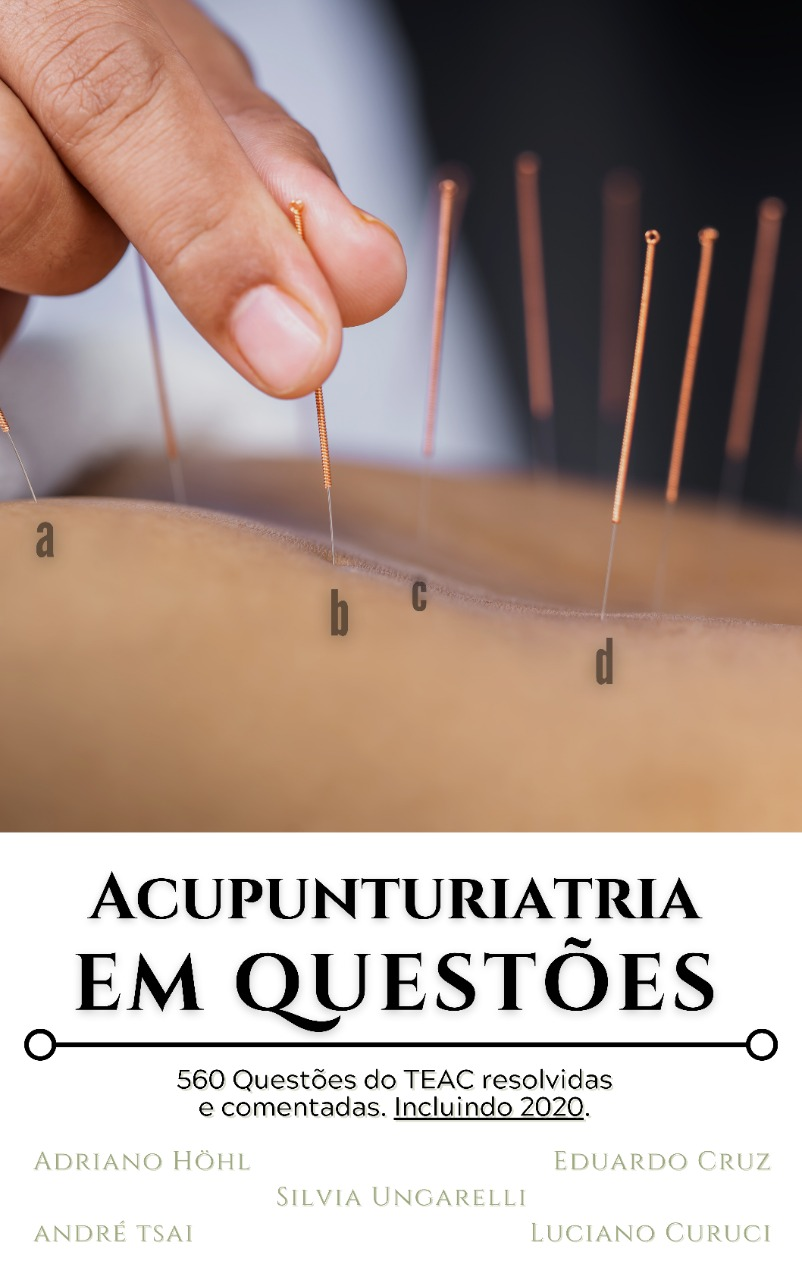
\includegraphics[width=8.5cm]{pix/coverimg.jpg} \\[0.3cm]
			% title
			%{ \huge \bfseries Acupuntura Médica em Questões} \\%[0.1cm]
			\HRule \\[0.3cm]
			
			% Optionally translator and publishing house
			% The Translator
			%\begin{minipage}{0.4\textwidth}
			%\begin{flushleft} \small
			%\emph{Translated by:}\\
			%Good Translator %here the translator
			%\end{flushleft}
			%\end{minipage}
			% Publishing House
			\begin{minipage}{0.4\textwidth}
				%\begin{flushright} \small
				\begin{flushleft} \small
					%\emph{Edição:} \\
					%\textsc{Eduardo Cruz} % here the publishing house
				\end{flushleft}
			\end{minipage}
			
		\end{center}
	\end{titlepage}
	
	
	
	%%%SIMPLE TITLEPAGE
	\maketitle 
	\thispagestyle{empty}
	\clearpage
	\setcounter{tocdepth}{6}
	
	%TOC
	\tableofcontents
	\listoftables
	%TUTAJ PISZ ALBO ZROB \INCLUDE{} LUB \INPUT{}


	%\input{lorem.tex}
	\part{Questões separadas por assunto}
	\chapter{Pontos de acupuntura}
	\begin{itemize}
	\item \noindent	\hyperlink{pontos 1}{2013-01}\\
	\item \hyperlink{pontos 2}{2013-02}\\
	\item \hyperlink{pontos 3}{2013-03}\\
	\item \hyperlink{pontos 4}{2013-04}\\
	\item \hyperlink{pontos 5}{2013-05}\\
\end{itemize}

	
	
\part{Capítulos introdutórios}	
% Capítulos introdutórios
\chapter{Prefácio}
O estudo da Acupuntura médica é bastante difícil e ao mesmo tempo encantador.
 
Iniciamo-nos na Medicina Tradicional Chinesa ainda no ano de 2017, em Goiânia - GO, onde descobrimos uma nova forma de ver a medicina em sua forma mais antiga da história. Deixamos para trás toda a tecnologia e toda a complexa farmacologia, potencializamos a nossa imaginação em busca deste conhecimento novo e de uma nova teoria que para muitos parece tão abstrata.  Um paradoxo entre uma Medicina tão simples, mas ao mesmo tempo tão complexa e que funciona tão bem que, com o tempo, nos mostrou a grande verdade do pensamento de Leonardo da Vinci quando  diz:  “A Simplicidade é o último grau de Sofisticação.”

A idéia desta obra surgiu durante a nossa especialização, em meio a dificuldades cotidianas como tempo para estudo, trabalho, compromissos familiares e o preparo para o esperado TEAC - prova de título de especialista em Acupuntura Médica, promovida pelo Colégio Médico Brasileiro de Acupuntura. A semente do trabalho foi plantada e germinada pela união e reunião de um grande número de alunos, até então especializandos. Neste momento, ainda alunos, reunimo-nos, dividimos e sistematizamos 12 anos de provas de título, para que assim pudéssemos compartilhar entre nós mesmos as questões comentadas que facilitariam nosso estudo.

O resultado da metodologia veio com a aprovação de 98\% da turma do CMA-Goiás, todos com médias de notas altas, além da primeira nota 10 em toda a história da prova de títulos em Acupuntura médica, feito alcançado por um dos autores desta obra, a Dra. Silvia Ungareli.

Selecionamos os últimos 07 anos e resolvemos refazer todas as questões novamente visando padronizar, aprimorar a didática e revisar por mais uma vez o conteúdo para que fosse possível aos novos especializandos, usufruir deste nosso trabalho.
 
Ressaltamos a importância do estudo sistematizado nos tratados e na referência bibliográfica de cada curso, pois nosso objetivo não é e nunca foi substituí-los e sim proporcionar uma ferramenta a mais para o entendimento e fixação do aprendizado, preparando para provas e concursos que o leitor possa participar.

Assim, a obra está organizada por questões e também por temas.
  
\part{Coletânea} Questões resolvidas e comentadas.

\chapter{TEAC 2013} TEAC 2013
\hypertarget{pontos 1}{2013-01}

 \section{QUESTÃO 01} - Usado para o tratamento da cefaléia e do torcicolo. Anatomicamente localizado em uma depressão entre o músculo esternocleidomastoideo e trapézio e, em posição profunda, no músculo esplênio da cabeça. Suprido pela artéria occipital e por um ramo do nervo occipital menor. Estamos nos referindo a qual ponto?  

a) Du Mai 16 
Situa-se na nuca, sob a protuberância occipital externa, na linha mediana do corpo, ou a um tsun acima da linha de inserção dos cabelos. Relaciona-se com os ramos cutâneos do nervo occipital terceiro (C) e com o nervo occipital maior (C2), ambos provindos do ramo dorsal.  
b) TA 17 
Situa-se posteriormente ao lóbulo da orelha, em uma depressão interóssea, localizada entre o processo mastoideo e o ramo da mandíbula. Relaciona-se, superficialmente, com o nervo auricular magno (plexo cervical) e, profundamente, com os nervos auriculotemporal (ramo do nervo trigêmeo) e com o nervo facial. 
c) VB 12 
Situa-se em uma reentrância óssea localizada posterior e abaixo do processo mastóideo. Fletir o pescoço para sua determinação. Relaciona-se com o nervo occipital menor (plexo cervical - C2). 
d) VB 20 
Trata-se de VB 20 que se situa em uma depressão óssea localizada entre o músculo esternocleidomastoideo e a inserção superior do músculo trapézio, ou na reentrância óssea localizada entre a protuberância occipital externa e o processo mastóideo ao nível de Du 16. Relaciona-se com o nervo occipital maior. 
 
A Alternativa correta é letra D.

\hypertarget{pontos 2}{2013-02}
TEAC 2013 \section{QUESTÃO 02} - Proximal ao processo estilóide do rádio, entre os tendões dos músculos braquiorradial e abdutor longo do polegar. Suprido pela veia cefálica e ramos da artéria e veia radial, inervado por um ramo do nervo cutâneo lateral do antebraço braço e por um ramo superficial do nervo radial. Indicado para disfunções respiratórias e dor de cabeça. Que ponto é esse?  

a) P 10  
Situa-se no meio do 1º metacarpo na linha da mudança da cor da pele. Relaciona-se com nervo cutâneo lateral do antebraço superficialmente e mediano profundamente. 
b) IG 5  
Situa-se numa reentrância no fundo da tabaqueira anatômica. Relaciona-se com o nervo radial. 
c) P 7  
Situa-se um e meio tsun proximais à prega ventral do punho, lateralmente a artéria radial. Relaciona-se com nervo radial.
d) IG 4 
Situa-se na metade do 2º metacarpo entre o primeiro e o 2º metacarpo. Relaciona-se com nervo mediano superficialmente e com o ulnar profundamente. 
 
\ textcolor{red}{A Alternativa correta é letra C. }
\hypertarget{pontos 3}{2013-03}
 \section{QUESTÃO 03}- Ponto com indicação ampla para enfermidades do baixo ventre, digestivas, urinárias e ginecológicas. Localizado a 3 cun inferior à cicatriz umbilical. Suprido pela artéria e veia epigástricas inferiores e por um ramo cutâneo anterior medial do nervo intercostal. A que ponto nos referimos? 
a) Ren Mai 4 
Trata-se de VC 4, ponto de saída dos três Yin do pé e ponto que harmoniza o   Aquecedor inferior, localizado na linha mediana anterior, 2 cun cranialmente à margem superior da sínfise púbica e 3 cun caudalmente ao umbigo. Fortalece e nutre os rins, o Jing, o útero, sendo importante em doenças ginecológicas e urológicas, fraqueza, dores e frio na região lombar, diarréia, incontinência fecal. 
b) R 13 
Situa-se a 3 tsun abaixo do centro da cicatriz umbilical e 0,5 tsun lateral à linha média anterior.
c) F 14 
Situa-se a 4 tsun laterais à linha média anterior, no sexto espaço intercostal.
d) E 29 
Situa-se a 4 tsun abaixo do centro da cicatriz umbilical e 2 tsun laterais à linha média anterior.
 
A Alternativa correta é letra A.
\hypertarget{pontos 4}{2013-04}
 \section{QUESTÃO 04} - Localizado no dorso da mão, entre o segundo e terceiro metacarpianos. Anatomicamente está situado no músculo interósseo do segundo metacarpiano, diretamente acima do nervo, artérias e veias digitais dorsais e palmares comuns, bem como do arco palmar profundo e ramos terminais profundos do nervo ulnar. Indicado para torcicolo, cefaléia, dor no ombro e braço. Qual dos pontos enumerados abaixo corresponde às referidas características? 

a) Yaotongxue (ponto extra) 
Localizam-se entre o 2º e 3º e entre o 4º e 5º metacarpos, na altura do corpo para a base. Indicado nas lombalgias agudas.
b) IG 3 
Situa-se em margem lateral (radial) do 2º metacarpo, em uma reentrância proximal à articulação metacarpofalângica. Na camada superficial, relaciona-se com os nervos digitais dorsais do ramo superficial do nervo radial e com os nervos digitais palmares próprios do nervo mediano. 
c) Baxie (ponto extra) 
Localiza-se entre as cabeças dos metacarpos. Relaciona-se com os ramos cutâneos e musculares dos nervos radial e ulnar. Indicado nas doenças articulares dos dedos, paresia dos dedos, cefaleia, torcicolo, dor de dente, garganta inflamada. 
d) Luozhen (ponto extra) 
O próprio nome significa torcicolo.  É um dos pontos extras importantes, situando-se no dorso da mão, meio tsun entre as cabeças do 2º e 3º metacarpos. Relaciona-se com os nervos digitais dorsais do nervo radial. 

A Alternativa correta é letra D. 
\hypertarget{pontos 5}{2013-05}
 \section{QUESTÃO 05}- Localiza-se na margem posterior do côndilo medial do joelho, na parte anterior da inserção dos músculos semimembranoso e semitendinoso e na margem do músculo sartório. Tem indicações no tratamento de disfunções do joelho, impotência sexual, vaginite. Que ponto é esse? 

a) BP 8 
Situa-se a cinco tsun distais à interlinha articular do joelho, sobre a margem medial da tíbia, ou a três tsun distais ao BP-9. Indicado em lombalgia, meteorismo, distensão abdominal e dos lados do abdome, dismenorreia, menorragia, menstruações irregulares, edema, polução noturna, dificuldade de micção e em todos os casos de formação ou de aumento da forma (tumores benignos, malignos, obesidade, artrose, etc). 
b) F 8 
Situa-se na face medial do joelho, na extremidade medial da prega poplítea, em uma depressão entre o tendão do músculo semitendíneo e o côndilo medial da tíbia. Para localizar o ponto, deve-se fletir o joelho e abduzir o membro inferior. Indicado nas afecções geniturinárias, vaginite, prostatite, nefrite, afecções do joelho, hemorragias intestinais, prolapso uterino, dores no baixo-ventre, disúria, prurido vulvar, dor no pênis, patologias hepáticas e biliares.
c) R 10 
Situa-se à margem medial da fossa poplítea, na prega poplítea, tangente à margem lateral do tendão do músculo semitendíneo. Faz a limpeza do Calor Perverso do Aquecedor Inferior e do Calor do Xue. Harmoniza o Qi contracorrente e é o ponto que rege as membranas. 
d) BP 9 
Situa-se em uma reentrância óssea que se encontra sob a margem inferior do côndilo medial da tíbia e o músculo gastrocnêmio. Indicado em todas as afecções encontradas na parte alta e interna do corpo, ocasionadas pela lesão da Energia Yin, plenitude nos lados do abdome, ascite ou edema, enurese noturna, incontinência urinária, espermatorréia, menstruação irregular, disenteria, distensão do abdome, retenção urinária, infecção urinária, gonalgia, dor nos genitais externos e lombalgia. 

A Alternativa correta é letra B.
 
 \section{QUESTÃO 06}- Os Canais Extraordinários se ramificam e intersectam um ou mais canais principais. A sintomatologia dos mesmos não é exclusiva, decorre de uma combinação de sintomas clínicos associados aos canais principais a que se ligam. O tratamento de doenças que afetam estes canais se faz através de pontos dos meridianos principais relacionados.
 Nesse sentido, é correto afirmar que: 

a) As doenças febris são comumente associadas ao Du Mai (Vaso Governador), e o principal ponto de interseção usado para seu tratamento é o Du 26. 
O correto seria Yang Wei Mai que se conecta aos três meridianos Yang do Pé e da Mão, com o Tai Yang, que controla a superfície do corpo e com o Shao Yang que tem relação com a síndrome intermediária. Esta é a razão da presença de frio ou febre quando há disfunção do Yang Wei Mai.  
b) Pelo fato do Du Mai suprir o cérebro e a região espinhal e intersectar o canal do Fígado no vértice, a obstrução do Qi neste canal pode resultar em sintomas como rigidez e dor ao longo da coluna vertebral. Na verdade, Du Mai recebe todos os canais yang da mão e do pé no vértice, em Du 20. Du Mai percorre a parte posterior do corpo e entra no cérebro. Uma anormalidade no Qi do Du Mai causa dor intensa ao longo da coluna vertebral e sensação de peso na cabeça. 
c) O Canal Yin Wei Mai (Vaso Conexão) é um dos canais que mais se relaciona com infertilidade e distúrbios do sistema urogenitais. 
O Canal seria Ren Mai que nutre e regula todos os meridianos Yin. No corpo humano, Qi pertence a Yang e Xue a Yin. A gestação, o parto, a menstruação e o corrimento vaginal estão intimamente relacionados a Xue (Yin), portanto dizemos que "o Ren Mai se encarrega do feto". 
d) O Canal Yang e Yin Qiao Mai (canal Yang e Yin do calcanhar) teem em comum a função de regular o movimento dos membros superiores. 
Na verdade, controlam membros superiores e inferiores. Yin Qiao Mai e Yang Qiao Mai controlam Yin e Yang em ambos os lados dos membros. O Yang Qiao Mai controla Yang Qi, enquanto o Yin Qiao controla Yin Qi. Eles controlam os meridianos Yin e os meridianos Yang nas faces medial e lateral da perna. 
 
A Alternativa correta é letra B. 

 \section{QUESTÃO 07}- Paciente de 42 anos queixa-se de dor aguda no pescoço e ombro, que piora com os movimentos. Acompanha-se de cefaleia cervical ou occipital. Diz que essa situação o está deixando irritado, com dificuldade para conciliar o sono e um tanto fadigado. Ao exame físico não apresenta nenhuma deformidade, no entanto, os movimentos ativos do pescoço são limitados e dolorosos. À palpação nota-se tensão muscular em trapézio e músculos paraespinhais. Radiografia em AP e perfil revelam alterações de espaço intervertebral e osteófitos entre C5 e C6 e C6 e C7. Na sua avaliação, qual seria o diagnóstico provável e a prescrição de pontos mais adequada para este caso? 

a) Hérnia de Disco Cervical; ponto principal extra Luozhen e pontos complementares: IG 4 e VB 38. 
Apesar de citar alterações do espaço intervertebral, a alteração é aguda, mostra comprometimento muscular e faltam dados concretos na clínica como sintomas de dor irradiada ou parestesias além de exames de imagem mais precisos que possam confirmar hérnia de disco cervical. 
b) Torcicolo ou Entorse Cervical; ponto principal extra Luozhen; pontos complementares: ID3 e VB 39. 
Corresponde ao torcicolo por contrações dolorosas da musculatura do pescoço, com limitação à rotação para um dos lados e posição antálgica. Segundo a MTC, essa alteração é causada por invasão de vento frio nos meridianos e colaterais locais ou pela estagnação de Qi e Xue ocasionada pela má posição da cabeça ao dormir ou trauma do pescoço ao esforço.  O tratamento visa à eliminação de vento e frio patogênicos e desobstrução dos meridianos.  
Lao Zhen (ou Luozhen) é um ponto extra que movimenta o Qi e o Xue na região do pescoço. O ID 3 é o ponto de confluência do intestino delgado com o Du Mai e o VB 39 é o ponto de influência da medula. Associados, podem regularizar o Qi e o Xue, relaxar os tendões e colaterais e promover analgesia. 
c) Luxação da Coluna Vertebral; ponto principal: Extra Yaotongxue; pontos complementares: ID 5 e VB 34 
Não existe história de trauma e nem mesmo alterações de imagem que possam reforçar esta hipótese.  
d) Espondilite Anquilosante; ponto principal extra Taiyang; pontos complementares: TA 5 e VB 34. 
Na espondilite anquilosante, a história é de evolução crônica e não aguda, acometendo mais de um segmento da coluna.  Não existem dados nas histórias que possam enquadrar o paciente nos critérios. 
 
A Alternativa correta é letra B.
 
 \section{QUESTÃO 08}- Paciente do sexo masculino, 42 anos, queixa-se de dor de instalação insidiosa há cerca de um ano. Trata-se de uma dor difusa, em peso, localizada na região lombosacra, sem irradiação para os membros inferiores, que melhora pelo repouso e exacerba-se aos esforços. À palpação, @incollection{maciocia1996fundamentos,
 	title={Os fundamentos da medicina chinesa: um texto abrangente para acupunturistas e fitoterapeutas},
 	author={Maciocia, Giovanni},
 	booktitle={Os fundamentos da medicina chinesa: um texto abrangente para acupunturistas e fitoterapeutas},
 	pages={658--658},
 	year={1996}
 }
 nota-se a musculatura da região lombosacra difusamente dolorida e reflexos profundos dos MMII sem alterações. Levando-se em consideração que a radiografia da coluna lombosacra foi de grande auxílio na elucidação diagnóstica, é correto afirmar, que nesse caso o diagnóstico e os pontos de acupuntura principais para o tratamento são respectivamente: 
  
a) Fratura de Vértebra Lombar. Pontos principais: B 40 e B 37   
Trata-se de dor de duração de 1 ano, envolvendo região lombosacra, em paciente jovem sem história de trauma, a qual teria uma evolução de melhora ou de complicação devido a etiologia mais agressiva como metástase, mas não evolução tão arrastada. Não seria a primeira opção de diagnóstico. 
b) Estenose de Canal Medular. Pontos principais: B 40 e VB 34  
No estreitamento do canal raquidiano artrósico, a dor lombar, às vezes, é noturna; outras vezes, a ela se associa ciatalgia uni ou bilateral intensa, que melhora ao sentar-se. Pode ser acompanhada de dor na panturrilha e de claudicação neurogênica intermitente. O processo doloroso piora ao caminhar, principalmente ladeira abaixo, e melhora ladeira acima, o que a diferencia da claudicação vascular, que piora ladeira acima. 
c) Tuberculose Espinhal. Pontos principais: B 40 e B 39   
A tuberculose espinhal geralmente se acompanha de sinais e sintomas próprios do processo infeccioso como febre baixa vespertina e evolução consumptiva, com progressão para   as vértebras vizinhas e aparecimento de comprometimento neurológico, o que não condiz com a história. 
d) Discopatia Degenerativa Lombar. Pontos principais: B 40 e B 60   
A discopatia degenerativa pode evoluir com a herniação do disco intervertebral para o canal espinhal, evoluindo ou não com sinais e sintomas neurológicos, conforme o grau de comprometimento da compressão de raízes nervosas. O fato de a dor melhorar com o repouso e piorar com as atividades físicas reforça a hipótese. Sob a óptica da MTC, trata-se de uma lombalgia Shao Yin que piora com fadiga, esforços físicos, mental e/ou sexual. O Tratamento baseia-se no uso de pontos locais associados a pontos à distância como R 2, R 3, B 40, B 60.  
O ponto B 40 é clássico para lombalgias e dorsalgias, podendo ser associado a B 60, B 23 e Yaoyan. 
 
A Alternativa correta é letra D.
 
 \section{QUESTÃO 09}- Paciente do sexo feminino, 40 anos, procura o ambulatório de acupuntura para tratamento de dor no ombro direito iniciada há cerca de um ano. Caracteriza-se por dor em pontada, de forte a moderada intensidade que piora ao movimento de abdução e irradia-se para a face anterolateral do braço (apresenta restrições aos movimentos ativos). Não apresenta parestesia ou choques. O sono é prejudicado devido ao agravamento da dor quando se deita sobre o lado comprometido. A radiografia do ombro mostra o acrômio curvado ou ganchoso, com diminuição do espaço da articulação glenoumeral. Na sua avaliação qual o diagnóstico mais provável? E qual é o melhor esquema de pontos para tratamento deste ombro doloroso? 

a) Hérnia Discal Cervical. Pontos principais: IG 14, IG 16, ID 8, TA 14, Extra Jianneiling. 
Nos casos de hérnia discal cervical teremos a descrição de uma neuralgia, com características diferentes da dor apresentada no caso acima, em que não há descrição de comprometimento neurológico. 
b) Capsulite Adesiva. Pontos principais: IG 16, ID 9, TA 14, Extra Jianneiling. 
A capsulite adesiva ou ombro congelado é um quadro clínico caracterizado por dor difusa em todo o ombro, que piora no período noturno e está associada a rigidez da articulação do ombro, com limitação de movimentos ativos e passivos. A história descrita não cita rigidez do ombro, mas apenas que há limitação ativa da articulação.
c) Síndrome do Impacto. Pontos principais: IG 15, IG 16, ID 11, TA 14, Extra Jianneiling. 
A alteração radiológica descrita é característica da síndrome do impacto tipo III. Sob a óptica da MTC, trata-se de uma ombralgia por estagnação do Qi e Xue nos meridianos Yang da mão. Os pontos locais de escolha podem ser IG 15, TA 14, ID 9, ID 10, IG 16, Naoshang, Jianneiling e ID 11, que são aplicáveis ao tratamento de todos os tipos de ombralgias, com a finalidade de aumentar o Qi Correto e dissipar os agentes perversos. 
d) Instabilidade Glenoumeral. Pontos principais: IG 12, IG 16, ID 11, TA 14. 
Na história não há descrição de luxação do úmero com dor intensa, associada a incapacidade de movimentar o braço, nem mesmo informação de que o paciente tem a sensação de que algo “saiu do lugar”.

A Alternativa correta é letra C.

 \section{QUESTÃO 10}- Paciente do sexo feminino, 32 anos, refere dor e disestesia na face lateral da coxa há 2 meses. A dor se irradia até a face lateral do joelho e, mais raramente, para a virilha ipsilateral. Tem a sensação de choque quando estende o quadril afetado. Ao exame físico não apresenta sensibilidade significativa ao nível do trocânter maior, nem restrições na rotação interna do quadril. Os reflexos nos membros inferiores são presentes e simétricos e as radiografias da pelve e quadril não mostram alterações. Analisando o quadro acima, qual seria a hipótese diagnóstica e a conduta adequada, respectivamente? 

a) Trata-se de um quadro de hérnia discal lombar e o meridiano comprometido é o do Baço 
Mesmo que se tratasse de uma hérnia discal, patologia que cursa geralmente com alteração dos reflexos e da sensibilidade, além da dor, o meridiano comprometido não seria o do Baço, por este ser medial, e sim o da Vesícula Biliar. 
b) Trata-se de um quadro de osteoartrite do quadril e o meridiano comprometido é o da Bexiga 
Pela localização da dor e disestesia ser na face lateral, o meridiano comprometido é o da Vesícula Biliar. 
c) Trata-se de um quadro de bursite trocanteriana e os principais meridianos afetados são Estômago e Fígado. 
O Quadro clínico não é compatível com a bursite trocantérica, que se caracteriza por dor crônica intermitente acompanhada de desconforto à palpação da região lateral do quadril e não de parestesia. A dor localizada à palpação do grande trocânter, área de inserção do tendão do glúteo médio, pode ser encontrada em todos os pacientes sintomáticos e pode ser reproduzida pela abdução ativa resistida e pela rotação externa da articulação, havendo a possibilidade de ser provocada ocasionalmente pela rotação interna. Como o comprometimento é da face lateral da coxa, o comprometimento é do meridiano da Vesícula Biliar. 
 
d) Trata-se de um quadro de meralgia parestésica; o principal meridiano afetado é o da Vesícula Biliar 
Trata-se realmente de um caso de uma mononeuropatia, mais especificamente a Meralgia Parestésica, patologia que se deve à compressão do nervo cutâneo lateral. Muito comum em mulheres atletas, se manifesta com sensações como dormência, formigamento, queimação, frio e dor nesta região da coxa. Além disso, há redução da sensibilidade e hipersensibilidade ao toque na região afetada, cujo tratamento é clínico conservador, associado à fisioterapia.  
Sob a óptica da MTC, por afetar a região lateral da coxa, trata-se de provável estagnação ou obstrução do meridiano da Vesícula Biliar, devendo-se usar pontos locais e à distância, visando estabelecer a circulação de Qi e Xue. 
 
A Alternativa correta é letra D. 

 \section{QUESTÃO 11}- Paciente do sexo masculino, 40 anos, procura ambulatório de acupuntura referindo dor no quadril esquerdo há um ano. A dor é de forte intensidade, em pontada e contínua, com irradiação para face lateral da coxa; piora ao movimento de levantar e sentar, e melhora quando deambula por pouco tempo (piora se permanecer andando por longo tempo). Não consegue dormir, pois a dor agrava quando se deita sobre o lado afetado. Ao exame físico, apresenta claudicação com a deambulação, sinal de Trendelenburg positivo, sensibilidade dolorosa aumentada acima da face lateral do trocânter e ausência de pontos gatilhos palpáveis. Não apresenta dor à rotação interna, mas refere dor discreta à rotação externa do quadril. Ao exame neurológico, os reflexos dos MMII estão presentes e simétricos. Radiografias da pelve e quadril esquerdo mostram a presença de osteófitos na face lateral do trocânter. Qual o diagnóstico provável e a prescrição de pontos mais apropriados para essa nosologia?
  
a) Síndrome dolorosa miofascial do músculo piriforme; pontos: VB 31, VB29, VB 25  
O caso não se enquadra na síndrome dolorosa miofascial do músculo Piriforme. A síndrome do piriforme (SP) é uma importante causa de dor na região glútea que pode frequentemente ser acompanhada de ciatalgia. Atualmente é descrita como uma forma de encarceramento do nervo isquiático que causa dor desde a região glútea à área de distribuição deste nervo, representando uma entidade clínica configurada não somente pela presença do quadro álgico, mas também por distúrbios sensitivos, motores e tróficos relacionados à distribuição radicular do nervo isquiático. 
b) Tendinite do tendão do glúteo médio; pontos: VB 30, VB 29, VB 39  
Na tendinite do músculo glúteo médio, a dor localiza-se na região do quadril (sobre o trocânter do fêmur), pode irradiar-se pela face lateral da perna e piora ao ficar muito tempo em pé, ao subir e descer escadas, ao caminhar ou ao correr. Pela localização do quadro álgico, trata-se de comprometimento do Meridiano da Vesícula Biliar, podendo ser usados pontos locais VB 29, VB 30 e pontos à distância como VB 34. O teste de Trendelenburg é um exame físico rápido que pode ajudar o terapeuta a avaliar qualquer disfunção do quadril. Um teste de Trendelenburg positivo geralmente indica fraqueza nos músculos abdutores do quadril: glúteo médio e glúteo mínimo. Um teste positivo é aquele em que a pélvis cai no lado contralateral durante uma perna única no lado afetado. Isso também pode ser identificado durante a marcha: a compensação ocorre ao lado flexionando o tronco em direção ao lado envolvido durante a fase de apoio na extremidade afetada.
c) Meralgia parestésica; pontos: VB 29, B 23, VB 34  
No caso da meralgia parestésica, o principal sintoma é a parestesia, em virtude da compressão nervo cutâneo lateral da coxa. 
d) Lombociatalgia; pontos: B 23, B 25, VB 30, VB 31, VB 41  
No caso da lombociatalgia, a dor inicia-se na região lombar e se irradia pelo trajeto do nervo ciático, ou seja, região glútea, posterior da coxa e perna podendo lateralizar ou medializar distalmente até o pé na dependência do dermátomo comprometido (raiz correspondente). A dor ciática é relatada pelos pacientes como “ferroada”, “fisgada” ou “sensação de choque” associada a parestesias e graus variados de déficit motor do(s) membro(s) inferior(es) bem como marcha claudicante. A associação com postura antálgica da coluna lombar em escoliose ou posição em flexo lombar é comum. A dor tem características mecânicas: piorando aos movimentos e esforços em geral e atenuando em repouso, posição fetal ou decúbito dorsal com quadris e joelhos fletidos. Há exacerbação da dor também à manobra de Valsalva (tosse, espirros e esforços para evacuação).

A Alternativa correta é a letra B.

\section{QUESTÃO 12}- Paciente do sexo feminino, 50 anos, queixa-se de dor localizada logo acima da tuberosidade medial do calcâneo esquerdo há oito meses. A dor melhora com repouso e é mais intensa ao despertar, quando dá os primeiros passos. Apresenta sensibilidade dolorosa 1 a 2 cm, distalmente, ao longo da fáscia plantar. A radiografia lateral do pé esquerdo para diagnóstico diferencial não mostrou nenhuma relevância. Qual o diagnóstico, a técnica e os pontos a serem prescritos? 
a) Fasciíte plantar. Os principais pontos são os dolorosos locais. Caso não melhore a dor, se faz uso dos pontos complementares: B 57, R 3 e B 60, com estímulo moderado a forte. 
Trata-se de um quadro clássico de fasciíte plantar, condição crônica caracterizada por dor na região plantar do terço posterior dos pés, dor à compressão da tuberosidade medial do calcâneo e história de dor nos primeiros passos do dia. Tratamento com AINES, palmilhas e acupuntura. Os pontos mais usados são: R 3, B 60, B 57 e pontos locais. 
b) Síndrome do túnel tarsiano. Os pontos principais são: B 57, R 1 e B 60. Caso não melhore a dor, usam-se os pontos complementares, que são os pontos dolorosos locais, com estímulo moderado a forte. 
Na síndrome do túnel do tarso, a dor é retromaleolar em queimação ou formigamento e algumas vezes no calcanhar plantar medial, podendo se estender-se ao longo da superfície plantar, bem como nos dedos dos pés. Embora a dor piore durante a permanência em pé e ao caminhar, pode ocorrer dor em repouso, o que a diferencia da fasciíte plantar. Sendo patologia de acometimento medial, presume-se o comprometimento dos meridianos Yin do Pé e pela topografia haveriam pontos mais indicados para o tratamento, como R 3, R 7, BP 4, BP6, entre outros. 
c) Ruptura traumática aguda da fáscia plantar; os pontos principais são: B 57, R 3 e B 62, não havendo indicação para o uso de pontos dolorosos locais devido a lesão da fáscia 
Na ruptura traumática aguda da fáscia plantar a dor é de aparecimento súbito, acompanhada de uma sensação de clique. Geralmente localiza-se na região medial da planta, afastada do calcanhar, com uma grande sensibilidade ao toque e dificuldade na marcha, acompanhada de edema e equimose ao longo da borda medial do pé. 
d) Osteoartrose da articulação do tornozelo; os pontos principais são: B 57, R 9 e B 60. Caso a dor não melhore, se faz uso dos pontos dolorosos locais com estímulo moderado a forte 
A osteoartrite da articulação tíbio társica cursa com dor na interlinha articular, associada ou não a aumento de volume (derrame articular) e limitação da amplitude de movimento articular, da função, do trabalho e das atividades de lazer. A etiologia pós-
traumática é a principal causa da osteoartrite de tornozelo. Ao exame radiológico, pode-se constatar diferentes graus de diminuição do espaço articular e formação de osteófitos, esclerose e cistos subcondrais.  
Alternativa correta é letra A.
\section{QUESTÃO 13}- Paciente com 40 anos, sexo feminino, com dor no joelho direito há um ano, foi encaminhada ao serviço de acupuntura pelo fato de não haver obtido melhora com uso de AINHs, corticoides e fisioterapia. Informa que a dor piora ao levantar pela manhã ou depois de um período de exercício contínuo, caminhadas ou corrida, fatores que a levam a claudicar. Localiza-se na face medial do joelho, ao nível da inserção conjugada dos músculos isquiotibiais. Ao exame físico não há restrições de movimentos, porém a movimentação do joelho é dolorosa. Não há instabilidades, travamentos ou outros sintomas mecânicos. As radiografias em AP, perfil e axiais não apresentaram alterações relevantes. Levando em consideração o quadro acima, podemos afirmar:  

a) Não deixa dúvidas que estamos diante de um quadro de artrite reumatóide de joelho. A acupuntura não trará benefícios à paciente, pois o tratamento indicado deve ser feito a base de metotrexato e hidroxicloroquina 
Apesar da rigidez matinal, não há sinais flogísticos e nem sorologia para que se possa confirmar o diagnóstico, nem tão pouco alterações radiológicas. Ainda que fosse, poderiam ser usados pontos de acupuntura para diminuição do processo inflamatório e da dor. 
b) O quadro clínico fecha o diagnóstico de tenossinovite de joelho. Os pontos indicados neste caso são: E 35 e Xiyan medial, B 40 e pontos dolorosos locais. 
O diagnóstico de tenossinovite é a principal suspeita diagnóstica pois cursa com dor à palpação da inserção muscular e que piora com atividade física, porém sem limitação da mobilidade, o que faz pensar em patologia extra-articular. Os pontos E 35, Xiyan medial e B40 são excelentes opções de associação de pontos locais para afecções de partes moles do joelho. 
c) Neste caso, é indispensável a RNM para afastar laceração de menisco medial que, caso comprovada, terá indicação imediata de cirurgia.  
A RNM é um exame de diagnóstico que poderá ser precedido pela radiografia e também pela ultrassonografia. Geralmente, no caso de lesão de menisco, ocorrem sinais flogísticos de dor e edema além da restrição de movimento.  O tratamento pode variar de fisioterapia até cirurgia, sendo a última terapia de exceção, não sendo de indicação imediata.  
d) Trata-se de um caso clássico de osteoartrite de joelho. Os pontos indicados são: E 35, E 36, Extra Heding e BP6. 
A ausência de alterações radiológicas e instabilidades já afastaria a hipótese de osteoartrite de joelho.  

A Alternativa correta é letra B.

\section{QUESTÃO 14}- Paciente de 43 anos, com queixa de dores articulares há cerca de dois meses. Informa que a dor surgiu de forma insidiosa, tem caráter migratório e de forma simétrica nas pequenas articulações (mãos e pés) e grandes articulações (tornozelos e joelhos). Apresenta rigidez articular prolongada, que é pior pela manhã, bem como aumento do volume articular. Sente-se fadigada e tem aversão ao frio. Ao exame físico, as articulações apresentam-se com edema, principalmente as articulações interfalangeanas proximais,
 e com limitação dos movimentos pela dor. Língua com revestimento branco e fino; pulso superficial. Nos exames laboratoriais o FR é negativo, VHS e PCR com valores aumentados, e os anticorpos antipeptídeos citrulinados (anti-CCP) são positivos. O hemograma apresenta-se com normocitose e discreta hipocromia. Radiografias das mãos mostram diminuição do espaço articular em falange metacarpofalangeana. Foi avaliada por um reumatologista que fez o diagnóstico e a encaminhou ao médico acupunturiatra para tratamento conjunto. Qual o diagnóstico feito pelo reumatologista e pelo acupunturiatra, respectivamente? 

a) Osteoartrite generalizada; caracteriza uma Síndrome Bi Frio. 
Apesar da aversão ao frio, não existe relato de melhora da dor com o calor ou piora da dor pelo frio e, mesmo o revestimento da língua sendo branco, o pulso não é tenso em corda, como deveria ser na invasão do frio patogênico.  
b) Polimialgia reumática; caracteriza uma Síndrome Bi Calor. 
Não há sinais flogísticos de rubor e calor que caracterizem a Síndrome Bi Calor e nem dor à palpação, língua com saburra amarelada ou pulso rápido. 
c) Lúpus eritematoso sistêmico; caracteriza uma Síndrome Bi Umidade. 
O caráter migratório da dor, já descartariam Bi Umidade, pois o próprio nome diz, “ Bi fixa”. Além disso, a língua não se encontra pegajosa e nem o pulso mole e escorregadio.  
d) Artrite reumatóide; caracteriza uma síndrome Bi Vento. 
Trata-se de um quadro de artrite reumatoide que geralmente tem início insidioso, com fadiga, anorexia, fraqueza generalizada e sintomas musculoesqueléticos vagos, e gradualmente manifesta seus sintomas específicos, tais quais poliartralgia simétrica, especialmente de mãos, punhos, joelhos e pés, com limitação de movimentos devido à dor e rigidez generalizada. O fator reumatóide é um auxílio diagnóstico utilizado, entretanto de pouca especificidade e nem sempre positivo. VHS e PCR evidenciam o caráter inflamatório da doença. Os anti-CCP têm uma sensibilidade semelhante e uma especificidade maior para artrite reumatoide que o FR. Há comumente anemia normocrômica e normocítica. À radiografia, nota-se perda de cartilagem articular e erosões ósseas. Sob a óptica da MTC, trata- se uma Síndrome Bi com estagnação de Qi e Xue e o caráter migratório da dor, por si só já evidencia a ação do vento. A aversão ao frio e língua com revestimento branco é decorrente da obstrução dos canais pelo frio e o pulso superficial, significa a luta do Wei Qi com fatores patogênicos.
     
A Alternativa correta é letra D.

\section{QUESTÃO 15}- Segundo o discurso preconizado pela Medicina Chinesa, qual seria o princípio de tratamento e os pontos mais adequados para o controle da dor das artropatias? 

a) Eliminar o patógeno responsável pelo quadro doloroso, fazendo circular o Qi e Xue (sangue) nos meridianos acometidos, bem como selecionar os pontos de acordo com as diferentes localizações das áreas da doença. 
Sendo a artropatia uma estagnação de Qi e Xue, seu tratamento consiste em eliminar o patógeno responsável pelo quadro doloroso, dissipando o vento e a umidade e eliminando o frio e o calor, revertendo a obstrução do Qi e Xue no meridiano acometido, além de utilizar pontos locais para a dor, podendo-se utilizar também os pontos Ah Shi. 
b) Não existem pontos específicos para eliminar o agente etiológico da síndrome dolorosa. São suficientes os pontos distais e locais nos meridianos acometidos 
Além dos pontos Ah Shi, pontos locais e pontos distais, existem sim pontos específicos gerais que atuam eliminando patógenos como vento, calor, frio e umidade.  
c) Numa síndrome dolorosa em que o agente etiológico é o frio, o princípio de tratamento é eliminar o frio através do uso de pontos específicos para essa finalidade. 
Numa síndrome dolorosa pelo frio, o princípio é dispersar e eliminar o frio e drenar os meridianos. 
d) Em uma síndrome dolorosa em que o agente etiológico é a umidade os pontos indicados para o tratamento, são: Du 14, IG 11, IG 4, F 3 
Para o tratamento do acúmulo de umidade usamos E 40, BP 9, VC 12 e VC 9. 
 
A Alternativa correta é letra A.
 
\section{QUESTÃO 16}- De acordo com seu conhecimento em tratamento de patologias álgicas com acupuntura, assinale a alternativa que apresente um conjunto de pontos adequados ao tratamento de dor localizada nos quirodáctilos?  

a) IG 4, IG 5, ID 5
ID 5 localiza-se na região ulnar do punho, utilizado principalmente para afecções do punho. IG 5 localiza-se no centro da tabaqueira anatômica, indicado para artrite na mão e punho.
b) IG 4, IG 11, TA 4  
IG 11 localiza-se na extremidade lateral da prega do cotovelo (cotovelo fletido), utilizado principalmente para inflamação e dor no braço e epicondilite lateral. TA 4 localiza-se na prega posterior do punho, entre a ulna e o carpo, utilizado principalmente para dor no punho, braço, ombro, cabeça e região lombar.
c) IG 3, ID 3 e os pontos extra Baxie 
As dores nos dedos das mãos devem-se ao acometimento por Energias Perversas Frio, Vento, Umidade e Umidade-Calor de um ou mais Canais de Energia da mão ou à deficiência do Shen Qi (Rins). Os pontos adequados para o tratamento da dor são os Ting dos Canais de Energia, pontos extras Baxie, Shangbaxie e Sifeng, IG 3, unir IG 4 a ID 3 ou a CS 8. Puncionar e estimular TA 5 e TA 2. Tonificar o Shen Qi (Rins) R 7. 
d) IG 4, ID 3, TA 4 e os extra Bafeng 
TA 4 localiza-se na prega posterior do punho, entre a ulna e o carpo, utilizado principalmente para dor no punho, braço, ombro, cabeça e região lombar. Ponto extra Bafeng, localiza-se no pé, nas extremidades proximais das quatro pregas interdigitais, utilizado principalmente para distúrbios no pé.
  
A Alternativa correta é letra C.

\section{QUESTÃO 17}- Paciente adulto jovem, com quadro epilético e psiquiátrico, procura tratamento com acupuntura motivado pelo insucesso na tentativa de controlar suas crises convulsivas com tratamento convencional. Fez uso de vários medicamentos e, atualmente, a droga utilizada é a Carbamazepina, que vem sendo administrada na dose máxima permitida, o que tem lhe gerado sono exagerado e alterações da função hepática. Refere também estar sentindo-se apático, um tanto depressivo e com certo grau de demência. Frequentemente, encontra-se falando consigo mesmo (solilóquio). O exame físico é praticamente normal. A inspeção evidencia língua com saburra branca e pegajosa e o pulso escorregadio. Bioquímica: AST (TGO) 50 mg/dl e ALT (TGP) 62 mg/dl; Hemograma: leucopenia, eosinofilia e trombocitopenia. De acordo com a MTC, o quadro desse paciente corresponde a qual diagnóstico sindrômico?
  
a) Fogo-mucosidade de Gan (Fígado)  
As manifestações clínicas do padrão são vertigens, dor em distensão na cabeça, rubor facial, conjuntiva hiperemiada, boca amarga e seca, irritabilidade e insônia, sono conturbado por sonhos, dor em queimação no tórax e hipocôndrios, constipação, urina amarela, tinidos, língua vermelha com revestimento amarelo e pulso em corda, rápido.
b) Estagnação do Qi de Gan (Fígado)  
As manifestações clínicas do padrão dor migratória e em distensão nos hipocôndrios e no baixo ventre, sensação de opressão torácica, tendência a suspirar, depressão ou raiva, globo histérico na garganta, bócio, massas abdominais, dor em distensão nas mamas, dismenorréia e/ou menstruação irregular ou amenorreia, pulso em corda.
c) Distúrbio de Fei (Pulmão) mucosidade 
As manifestações clínicas do padrão são tosse com expectoração espessa profusa e branca de fácil eliminação, congestão torácica. A dispnéia com ruído de catarro na garganta também é frequente. Língua pálida com revestimento branco e pegajoso e pulso escorregadio.
d) Orifícios de Xin (Coração) obstruídos pela mucosidade
As manifestações clínicas do padrão são depressão mental, apatia, demência, solilóquio, alteração do comportamento, coma repentino, ruído de saliva e catarro na garganta, desvio conjugado dos olhos para cima, convulsões, língua com revestimento branco pegajoso, pulso escorregadio.
O quadro apresenta sintomas de estagnação do Qi do Gan, acúmulo de mucosidade e alterações da mente. A apatia e o falar consigo mesmo (solilóquio) seria explicada pela estagnação do Qi do Gan, associado à ação da mucosidade no Xin. As crises convulsivas se dão pela disfunção do Xin e pela mucosidade em seu meridiano, pela agitação do vento do Gan, que ascende junto com a mucosidade para obscurecer o Xin, causando perda de consciência abrupta, ruído de saliva ou catarro na garganta. Como o Gan controla os tendões, a agitação do vento leva ao desvio conjugado dos olhos para cima e à convulsão das quatro extremidades. A ascensão abrupta do Qi do Gan causa acúmulo de mucosidade na garganta, provocando ruídos característicos de crise epiléptica. 

A Alternativa correta é letra D. 

\section{QUESTÃO 18} - A SOP (Síndrome dos ovários polimicrocísticos) é frequente em mulheres jovens na idade reprodutiva, com prevalência de 5 a 10\%, sendo as adolescentes acometidas em 26\%. Na faixa etária de 19 a 45 anos é responsável por aproximadamente 75\% dos casos de infertilidade e 80\% de hirsutismo. A acupuntura vem demonstrando, através de variados ensaios experimentais e clínicos, ser uma técnica bastante promissora no tratamento desta síndrome de anovulação crônica. Considerando o que foi descrito, uma paciente com SOP pode apresentar oligomenorreia (menstruações com intervalos longos), hiperandrogenismo (acne e hirsutismo) e infertilidade. Segundo o discurso da MTC, quais seriam os Zang-Fu (órgãos e vísceras), que quando em desarmonia, são responsáveis por esses sintomas? 

a) Pi (Baço) e Gan (Fígado) 
Apesar de Pi participar junto com Gan e Shen do processo de fertilidade, os principais são Gan e Shen, que controlam diretamente Chong Mai e Ren Mai. 
b) Gan (Fígado) e Wei (Estômago) 
Wei não tem relação direta com a síndrome acima exposta.
c) Xin (Coração) e Shen (Rim) 
Xin não tem relação direta com os sintomas apresentados. 
d) Gan (Fígado) e Shen (Rim) 
A fertilidade e o controle da menstruação são dependentes do equilíbrio de Chong Mai e Ren Mai, ambos subordinados a Shen e Gan. Se ocorrer deficiência de Jing no Shen e Xue de Gan esses dois Zang não conseguirão nutrir o Ren Mai e Chong Mai, ocorrendo desde irregularidade menstrual até oligomenorreia. A acne é explicada pela ação do fogo perverso, formado pela estagnação de Gan. 

A Alternativa correta é letra D.

\section{QUESTÃO 19}- Uma paciente de 35 anos, com diagnóstico de SOP (Síndrome dos Ovários Polimicrocísticos), procura o ambulatório de acupuntura com história de várias tentativas para engravidar com indutores da ovulação (citrato de clomifeno), associado à anti hiperglicemiantes (metformina), sem sucesso. Não quer recorrer à fertilização assistida antes de tentar tratamento com a acupuntura. Na anamnese, revela atraso menstrual com sangramento escasso e escuro, dor no baixo ventre com sensação de frio, sensação de frio nos membros e corpo, diurese abundante e clara. Esporadicamente, a dor se irradia para as costas, acompanhada de fraqueza nas pernas. Ao exame físico, língua pálida com revestimento fino, pulso profundo e lento.  
Quais são os melhores pontos e técnica, respectivamente, para tratar esta paciente?  
a) Ren Mai 2, Ren Mai 6, Du 4, E 29, B 23 e Extra Yaoyan. Método de tonificação em todos os pontos e pode-se usar moxabustão.  
Pontos descritos são usados para tratamento da infertilidade causada por retenção de frio no útero. A invasão do frio exterior ou do frio interior causada por insuficiência de Yang provoca estagnação e obstrução do fluxo de Qi e Xue, ocasionando atraso menstrual e diminuição do fluxo sanguíneo, menstruações com sangramento escuro, dores com sensação de frio no baixo ventre, frio ou hipotermia no corpo e nos membros. A dor nas costas, a fraqueza das pernas e a diurese clara e abundante são secundárias à insuficiência de Yang do Shen, que deixa de exercer sua função de aquecimento e provoca disfunção do Qi. A língua pálida com revestimento fino e o pulso filiforme são sinais da síndrome de frio. O princípio de tratamento é aquecer o útero para dissipar o frio. Pontos RM 7, RM 2, DM 4 e RM 6. O Ren Mai e o Du Mai passam pelo útero. RM 7, RM 2 e o DM 4 podem ser utilizados para aquecer e dissipar o frio no útero. A moxibustão em RM 6 pode tonificar o Yang de modo a reforçar a ação que dissipa o frio aquecendo o útero. Se ocorrer atraso menstrual, acrescentar E 25 e E 29. B23 e YaoYan (EX-DL7) para dores nas costas e fraqueza das pernas. Agulhar os pontos 1,0 a 1,5 tsun, com método de tonificação, podendo-se utilizar moxibustão.
b) Ren Mai 3, E 30, R 14, BP 6 e E 40, BP 8, F 3, PC 6. Método de sedação em todos os pontos e pode-se aplicar moxabustão. 
Pontos descritos são usados para tratamento da infertilidade causada por estagnação de mucosidade de Xue, cujas manifestações incluem atraso menstrual, fluxo menstrual obstruído com coágulos, plenitude do tórax e hipocôndrio, agitação e irritabilidade, ou obesidade, tontura, palpitação, leucorreia espessa e pegajosa. Método de sedação sem moxabustão.
c) B 23, R 13, IG 11. Método de tonificação em todos os pontos e a moxabustão não deve ser usada  
Pontos B 23, R 13 e R 2 são usados para tratamento da infertilidade causada por deficiência do Shen, cujas manifestações incluem oligomenorreia com sangramento pálido, compleição pálida, fraqueza física generalizada, lassidão mental, tontura e tinnitus. Pode-se utilizar moxibustão. IG 11 não é descrito como ponto para tratamento de infertilidade.
d) Ren Mai 4, E 13, extra Zi Gong, BP 6 e E 36. Método neutro e pode-se usar moxabustão  
Pontos descritos são usados para tratamento da infertilidade causada por deficiência de Xue, cujas manifestações incluem oligomenorreia com sangramento pálido, compleição pálida, fraqueza física generalizada, lassidão mental, tontura e tinnitus. 
 
 
A Alternativa correta é letra A.

 \section{QUESTÃO 20}- Na MTC, o tratamento prioriza o doente e não apenas a doença. Busca integrar os diversos aspectos relacionados à natureza humana, dando ênfase especial ao aspecto emocional como fator de adoecimento. Nessa dinâmica, lista sete emoções básicas que quando em desarmonia podem gerar desequilíbrios orgânicos. Baseado nesses critérios assinale qual repercussão sofreria um indivíduo submetido a atos de violência verbal ou física, numa determinada fase da vida, com introjeção de um sentimento raivoso.  

a) Inversão do Qi do Gan (Fígado) para cima  
A raiva é a emoção ligada ao Gan. O Gan é o responsável pela circulação harmônica do Qi.  A raiva promove a estagnação do Qi no Gan, que, ao invés de ser distribuído   harmonicamente, se acumula e ascende de forma patológica, levando a sintomas por promover desarmonia dos outros Zang Fu ou pelas alterações que promove em seu meridiano e no meridiano da Vesícula Biliar. A ascensão anormal do Qi do Gan pode provocar a subida do Xue e o fechamento dos orifícios limpos, resultando em síncope.
b) Provocaria dispersão do Qi de Xin (Coração)  
O coração, Zang que controla a mente, é regido pela emoção da alegria e pode ser desequilibrado pela euforia, que provoca o alentecimento do Qi e do Xue e a dispersão do Qi do Xin, levando ao transtorno mental, à incapacidade de se concentrar e até mesmo à confusão mental.  
c) Enfraquecimento do Qi do Shen (Rim)  
O Zang Shen é desequilibrado pelo medo. O medo exagerado provoca o afundamento ou desabamento do Qi, enfraquecendo o Qi do Shen, levando a incontinência urinária e fecal.
d) Causaria estagnação do Qi e enfraquecimento do Xin (Coração) e o Pi (Baço) 
O distúrbio das atividades funcionais do Qi provocado pela emoção relacionada ao Xin já foi descrito. O excesso de pensamento causa estagnação do Qi e enfraquece o Xin e o Pi. O enfraquecimento do Qi do Pi causa incapacidade do Pi de transformar, distribuir e transportar alimentos efetivamente, ocasionando plenitude e distensão no epigástrio e abdome, anorexia e diminuição do apetite.

A Alternativa correta é letra A. 
 
 \section{QUESTÃO 21}- Paciente de 23 anos procura o ambulatório de acupuntura com quadro de enurese noturna. Refere que, até então, os médicos não haviam encontrado nenhuma causa orgânica que justificasse esta constrangedora disfunção. No interrogatório, apresenta micção frequente, com urina abundante e clara, ou gotejamento. Queixava-se de fadiga e dor cansada em região lombar e joelhos. Como antecedentes apresentava: menarca aos 16 anos; Gesta I, Para 0; um aborto espontâneo. Ao exame ginecológico, não apresentava nada relevante. Sua língua mostrava-se pálida com revestimento branco e, à palpação, o pulso se apresentava profundo e fraco. Na sua avaliação, de acordo com a MTC, qual seria o diagnóstico sindrômico adequado ao quadro acima descrito? 
 
a) Deficiência do Yin do Shen (Rim)  
Não há sintomas de deficiência de Yin de Shen tais como vertigem e tinidos, insônia ou abundância de sonhos, polução noturna, irregularidade menstrual e sangramento uterino, emagrecimento, cabelos secos e sem brilho, febre, transpiração noturna, sensação febril ou calor nos cinco Xin, garganta seca, rubor malar, língua vermelha com fluido escasso e pulso filiforme e rápido. 
b) Deficiência do Qi do Pi (Baço)
Não há sintomas relacionados ao Pi (distensão abdominal), tais como anorexia, distensão abdominal agravada após as refeições, fezes amolecidas, membros fracos, respiração curta, indisposição para falar, compleição pálida e macilenta, emagrecimento, língua pálida com revestimento branco e pulso moderado, lento e fraco.  
c) Umidade e Calor de Pangguang (Bexiga)  
Não há sintomas de dor, peso ou queimação na bexiga, e nem sintomas gerais relacionados a umidade e calor.   
d) Deficiência do Qi de Shen (Rim)  
A deficiência do Qi do Shen está presente em idosos ou em jovens com deficiência congênita e excesso de atividade sexual. Quando o Qi do Shen se toma deficiente, a face e os ouvidos não são nutridos suficientemente pelo Qi e pelo Xue, ocasionando compleição pálida, fadiga e hipoacusia. Quando os ossos não são nutridos e aquecidos pelo Qi do Shen, ocorre dor e lassidão nos joelhos e na região lombar. A hipofunção do Panguang, decorrente da deficiência do Qi do Shen, resulta em micção frequente de urina volumosa e clara, ou ainda em incontinência urinária. O enfraquecimento do controle da micção por parte do Qi deficiente do Shen acarreta a micção em gotejamento. Não possibilitando o controle do Pangguang, a deficiência do Qi do Shen origina sua disfunção, que é marcada pela enurese, encontrada principalmente em crianças ou em jovens com insuficiência congênita. À noite, o Yin Qi é abundante e o Yang Qi é deficiente. Por conseguinte, o paciente cujo Qi do Shen é deficiente tem poliúria à noite. O Jing é armazenado no Shen, e sua preservação é responsabilidade do Qi do Shen. A deficiência do Qi do Shen compromete a habilidade do Shen de preservar sua essência (Jing), ensejando espermatorreia e ejaculação precoce. Quando o Qi do Shen está tão deficiente que causa perda do controle do Qi do Dai Mai ou não consegue nutrir o Ren Mai, ocorre leucorreia líquida ou fina e abortamento. A língua pálida com revestimento branco e o pulso profundo e fraco indicam deficiência do Qi do Shen.

A Alternativa correta é letra D.
 
 \section{QUESTÃO 22} - Paciente de 34 anos, sexo feminino, com dor epigástrica em queimação acompanhada de regurgitação ácida. Diz ter fome excessiva, e às vezes vômito pós-prandial imediato. Refere, também, halitose e inflamação gengival com sangramento a escovação. Costuma ter maus hábitos alimentares preferindo alimentos gordurosos, picantes e acres. Tendência à constipação intestinal. Ao exame físico apresentava dor à palpação profunda do epigástrio, língua vermelha com revestimento amarelo; PA: 120/80 mmHg e FC 88 bpm. Exames complementares: radiografia de tórax normal; ECG (eletrocardiograma) normal, função hepática normal e colesterol de 280 mg/dl. A endoscopia digestiva alta foi inconclusiva. A pH-metria nas 24h fechou o diagnóstico. Qual seria o provável diagnóstico nosológico e sindrômico segundo as avaliações pela Medicina ocidental e MTC, respectivamente? 
 
a) Angina pectoris, Estagnação do Xue (Sangue) de Xin (Coração)  
Na estagnação de Xue de Xin, em razão da deficiência de Yang do Xin, Xue de Xin não pode ser aquecido e movido, produzindo frio no seu interior, que bloqueia o Xin Xue nos vasos e impede seu fluxo, e em casos mais graves, obstrui os vasos do Xin provocando palpitação, corpo e membros frios, dor precordial aguda e alterações da mente. 
b) Esofagite de Refluxo, Calor em Wei (Estômago)  
Hiperatividade de fogo do Wei refere-se a condição patológica em que o fogo do Wei ascende ao longo do meridiano devido ao excesso de calor acumulado no Wei. O fogo do Wei é provocado por calor patogênico externo, ingestão excessiva de alimentos ácidos ou oleosos, ou álcool, ou estresse emocional que afeta o Gan e produz fogo. Fogo do Wei inicialmente causa uma hiperfunção deste em digerir alimentos, e então provoca uma sensação desconfortável no Wei, e o aumento de apetite. Fogo do Wei vigoroso e movimento ascendente de Qi do Wei podem provocar gosto amargo, sede, náusea, vômitos ácidos e biliosos, e constipação. O Calor excessivo no Wei acarreta aumento da velocidade da digestão o que acarreta fome excessiva. Exaure também os líquidos corpóreos, tomando insuficiente a umidificação do Da Chang, causando constipação. A língua vermelha com revestimento amarelo indica a presença de calor. Hiperatividade de fogo do Wei ao longo do meridiano provoca inflamação e dor nos lábios, boca, gengivas e bochechas, e uma preferência por frio e aversão ao calor.
c) Megaesôfago Chagásico, Deficiência do Yang de Wei (Estômago)  
Não existe história de disfagia para caracterizar megaesôfago chagásico. Frio no Wei (Wei Han) em geral, é causado por patógeno frio externo invadindo o Wei, dieta inadequada (comer alimentos crus ou frios, em demasia, pode afetar o Qi de Wei), insuficiência congênita causando produção de frio interno, ou consumo de Qi do Wei por doença crônica. As condições patológicas de frio no Wei incluem: consumo de Qi do Wei e estagnação de frio resultando em dor fria no Wei melhorada por pressão, e aversão ao frio; vômitos de fluido claro e inapetência, já que o alimento não pode ser transformado e digerido pelo Wei; descontrole de Qi do Wei em descender causa ascensão anormal de Qi do Wei, provocando distensão e pressão no epigástrio e abdome, eructações, náusea e vômitos. 
d) Síndrome do Intestino Irritável, Desarmonia entre Gan (Fígado) e Wei (Estômago)  
Não existe história de diarreia alternada com constipação e nem mesmo sintomas de Gan tais como dor em distensão nos hipocôndrios e no baixo ventre, dor migratória, tremor nos membros e no corpo, irritabilidade e doenças oftalmológicas, além de pulso em corda.
 
A Alternativa correta é letra B.

 \section{QUESTÃO 23}-  Paciente de 32 anos , solteira, com queixa de irregularidade menstrual há seis meses, com padrão hipermenorrágico (duração e quantidade aumentadas), que após problemas de saúde na família e grande preocupação com seus estudos, apresentou progressivo agravamento. Além da sua queixa principal, apresentava também: palpitação, amnésia, insônia com muitos sonhos, apetite diminuído, fezes amolecidas e distensão abdominal. Frequentemente notava o aparecimento de equimoses no corpo sem causa aparente. Procurou o hematologista para investigar uma possível disfunção hematológica, sem sucesso. Ao exame físico mostrava compleição doentia, mucosas descoradas +/+4, língua pálida e mole, pulso filiforme e fraco. O exame ginecológico não mostrou nada de relevante. USG transvaginal normal, $\beta$-HCG negativo, hemograma: eritropenia e hipocromia leves. 
De acordo com o quadro clínico descrito acima é correto afirmar? 
 
a) Trata-se de um sangramento uterino anormal (SUA) por adenomiose em decorrência da deficiência do Qi de Shen (Rim) 
A ultrassonografia normal praticamente afasta adenomiose e não há sintomas relacionados a Shen, tais como lassidão e dor nos joelhos e na região lombar, tinidos, diminuição da audição, embranquecimento dos cabelos e alopecia, menstruação escassa e amenorreia. 
b) Trata -se de SUA por disfunção hormonal, que é típica nesta faixa etária. De acordo com o diagnóstico pela MTC, mostra claramente o quadro clínico de uma síndrome complexa de Deficiência Conjunta do Xue (Sangue) de Xin (Coração) e do Qi do Pi (Baço) 
Tendo-se em vista os exames normais, por exclusão pensamos em disfunção hormonal. Sob a ótica da MTC, trata-se de uma Deficiência de Xue de Xin (palpitação, amnésia, insônia com muitos sonhos, língua pálida, pulso filiforme), associado a Deficiência de Qi do Pi (apetite diminuído, fezes amolecidas e distensão abdominal, aparecimento de equimoses no corpo sem causa aparente, língua mole e pulso fraco e filiforme). 
c) Não se pode afirmar nada porque as informações são insuficientes para chegar ao diagnóstico nosológico e sindrômico
A história é rica em informações clínicas, sob ponto de vista ocidental e da MTC. 
d) Trata -se de um caso de SUA por hiperprolactinemia. Preenche os sintomas e sinais de uma síndrome complexa de deficiência do Yang de Xin (Coração) e de Yang de Shen (Rim) 
Apesar de não ter sido relatado exame alterado de prolactina, a hiperprolactinemia se acompanha de amenorreia e não de hipermenorragia. O paciente não apresenta quadro de frio nos membros e em região lombar, e o pulso e língua não são condizentes com deficiência de Yang. 

A Alternativa correta é letra B.

 \section{QUESTÃO 24}- Paciente jovem, com 25 anos, procura o ambulatório de acupuntura para tratamento de uma dor pélvica de forte intensidade, que atrapalha suas atividades diárias, levando a um grande absenteísmo profissional. O problema teve início durante um período menstrual e progressivamente foi se tornando mais intenso e perdurando por quase todo o ciclo. A dor se irradia, antes ou durante a menstruação, para a região lombar, agrava-se pela pressão e é aliviada pela aplicação de calor. A menstruação é escassa, com sangue escuro e frequentemente com coágulos. Fez uso de contraceptivos orais, inibidores da aromatase e de análogos do GnRH, com discreta melhora. Não fez uso AINH (Antiinflamatórios não hormonais), porque é alérgica. A laparoscopia foi decisiva para o diagnóstico. Na sua avaliação do quadro álgico acima, qual afirmativa está correta? 

a) A dor pélvica crônica é secundária a Síndrome do Cólon Irritável. Os pontos F 3, F 13, VB 34 e E 36 seriam um bom esquema de tratamento para essa disfunção sindrômica 
Não há sintomas de diarreia alternando ou não com obstipação, ou outros sintomas relacionados a cólon irritável. 
b) A dor pélvica crônica é secundária a Retocolite Ulcerativa. De acordo com a MTC, deve-se a Estagnação do Qi de Gan Fígado) 
Não há sintomas de alterações intestinais e nem tão pouco sintomas de Gan, tais como dor em distensão nos hipocôndrios e no baixo ventre, dor migratória, tremor nos membros e no corpo, irritabilidade e doenças oftalmológicas, além de pulso em corda.
 c) A Endometriose é o provável diagnóstico etiológico. De acordo com a MTC, o diagnóstico sindrômico é obstrução por Umidade e Frio.  
Trata-se de dor forte, no período menstrual, que tem se prolongado e piorado, o que, pela medicina ocidental, leva à hipótese de endometriose. Sob a ótica da MTC, trata-se de dor intensa no Aquecedor Inferior, com características de dor em plenitude por excesso de fator patogênico, que, no caso, causa estagnação junto com a umidade obstruindo e estagnando o Qi e Xue no Aquecedor Inferior, no Chong Mai e no Ren Mai, originando uma dor fria no baixo ventre. Como existe um excesso de frio e umidade (plenitude do fator patogênico), a dor piora à pressão do abdome e como é devida ao frio, melhora com o calor. A escassez da menstruação e o sangue coagulado são devido à estagnação e contração devido ao frio e à obstrução do meridiano.  
d) Síndrome da Bexiga Dolorosa é o provável diagnóstico etiológico. De acordo com a MTC, o diagnóstico sindrômico é obstrução por Umidade e Calor no Jiao Inferior. 
Não há sintomas que caracterizem diagnóstico de bexiga dolorosa tais como dor pélvica crônica (com duração superior a 6 meses), urgência miccional, aumento da frequência urinária durante o dia e a noite, dor durante a relação sexual, sensação constante de bexiga cheia e infecções urinárias recorrentes. No caso de umidade calor na bexiga, ocorre micção frequente e urgente, sensação de queimação na uretra, urina escassa e amarela (concentrada), sensação de distensão e plenitude no baixo ventre acompanhadas de febre e dor lombar, hematúria ou cálculos urinários, língua vermelha com revestimento amarelo e pegajoso e pulso escorregadio e rápido.
 
A Alternativa correta é letra C.
 
 \section{QUESTÃO 25}- O corrimento genital é a principal queixa entre as pacientes que procuram atendimento médico, seja no serviço público ou privado. Muitas vezes é mal diagnosticado e tratado. O corrimento crônico de causa não sexualmente transmissível é um verdadeiro desafio ao clínico e ginecologista. Ele é decorrente do desequilíbrio da microbiota vaginal, secundária à higiene precária, baixa imunidade, maus hábitos alimentares e uso de medicamentos que alteram esta flora. Para uma paciente com queixa de corrimento branco e fino, fadiga nos membros e tontura, qual seria a sua proposta de tratamento? 

a) Pontos principais: VB 26, BP 6, Ren Mai 6. Pontos complementares: E 36 e Ren Mai 4; orientação higiênica e alimentar. 
Sob a ótica da MTC, as leucorreias são devido a uma fraqueza de Chong Mai e Ren Mai, e a uma perda da função de contenção de Dai Mai. A causa profunda pode ser uma fraqueza do organismo, uma estafa ou um acúmulo de mucosidade. A leucorréia branca e clara denota um padrão de frio por deficiência de Yang do Baço ou do Rim, ou frio-umidade exterior ou estagnação do Qi do Fígado. A consistência fluida sugere um padrão frio umidade. Tontura e fadiga nos membros evidenciam deficiência de Qi e Xue. Pontos escolhidos RM 4, VB 26, BP 6, acrescentar na leucorreia branca RM 6 e BP 9. VB 26 harmoniza o Yong Qi (Nutrição) e o Canal de Energia Dai Mai, tonificando o Gan e o Shen, harmonizando e eliminando a umidade do aquecedor inferior, além de aumentar o Qi do Chong Mai. BP 6 harmoniza, fortalece e tonifica o Pi, tonifica o Shen Qi e a Essência, harmoniza a circulação de Qi e de Xue (Sangue), tonifica o Qi e o Xue (Sangue), harmoniza o Qi do útero e da próstata, dissolve a Umidade e a Umidade Calor, drena a Umidade e a Umidade Frio. RM 6 tonifica o Shen Qi e o Yuan Qi, harmoniza e aquece o aquecedor inferior e o Ren Mai, tonifica o Qi, o Xue (Sangue) e o Yang Qi, dispersa a Umidade, a Umidade Calor e refresca o Calor do Xue (Sangue). RM 4 fortalece o Yin Qi e o Yang Qi e o Yang do Rim, aquecendo o frio, aumenta o Qi e o Xue, harmoniza e aquece o Qi do útero e fortalece o aquecedor inferior, dispersa a Umidade, a Umidade Frio e a Umidade Calor, harmoniza o Qi do Chong Mai e do Ren Mai. E 36 regulariza, harmoniza e fortalece o Qi do Pi, faz circular o Qi e o Xue (Sangue), transforma a Umidade e a Umidade Calor, drena a Umidade e a Umidade Frio, dispersa o Vento e o Frio. 
b) Não se deve tratar este tipo de corrimento vaginal com acupuntura, pois o uso de antimicrobianos tem se mostrado de muita eficácia. 
O uso de antimicrobianos para tratamento da leucorreia está indicado quando há presença de infecção com sintomas tais como corrimento amarelado, acinzentado ou esverdeado, presença mau odor (especialmente após a relação sexual ou menstruação), queimação ou ardor, dispareunia e prurido local. Sob a ótica da MTC, o prurido vulvar se deve à presença de Umidade Calor infundindo para baixo, incluindo os seguintes sintomas: dor vaginal, às vezes com corrimento amarelo e abundante, angústia, insônia, agitação, gosto amargo e pegajoso, distensão abdominal e urina concentrada. 
c) Pontos principais: F 2 e BP 9. Pontos complementares: E 36 e Ren Mai 4; orientação higiênica e alimentar 
Pontos principais para tratamento da leucorreia (provocada pela Umidade Frio) descrita no enunciado estão citados no comentário da letra A. F 2 tem indicação para tratamento de prurido genital.
d) Os pontos principais: F 3, BP 6 e IG 4; os pontos complementares: E 36 e Ren Mai 4; apenas orientação higiênica é necessário. 
Pontos principais para tratamento da leucorreia (provocada pela Umidade Frio) descrita no enunciado estão citados no comentário da letra A. IG 4 não tem, dentre suas inúmeras funções, indicação para tratamento de leucorréia.

A Alternativa correta é letra A.

\section{QUESTÃO 26} - Sabe-se que o tratamento do zumbido (tinnitus) é um grande desafio para o clínico. A acupuntura é uma arma a mais na tentativa de minimizar esse desagradável sintoma. Selecione abaixo o conjunto de pontos mais indicado para o tratamento dessa disfunção. 
a) Pontos principais: TA 17, VB 20 e TA 3. Pontos complementares: F 2, E 40, F 13, B 2 
Pontos principais e complementares para tratamento do zumbido estão citados no comentário da letra C. F 13 é ponto Mu (alarme) do Pi e de influência dos Zang sendo importante para quadros que resultam da hiperdominância de Gan em Pi (sintomas digestivos causados pelo estresse). B 2 é um ponto que beneficia os olhos.
b) Pontos principais: IG 19, VB 20 e TA 15. Pontos complementares: F 2, E 40, R 3, B 40 
Pontos principais e complementares para tratamento do zumbido estão citados no comentário da letra C. IG 19 é um ponto utilizado para tratamento de obstrução nasal, epistaxe, paralisia facial, desvio da boca e rinite. TA 15 é um importante ponto para tratamento das afecções do ombro e para relaxar (Mal de Atlas). B 40 é um importante ponto para as lombalgias agudas.
c) Pontos principais: TA 17, B 20 e TA 3. Pontos complementares: F 2, E 40, R 3, B 23 
Em geral, as causas do zumbido decorrem de um desequilíbrio do Qi nos ouvidos, em virtude de um quadro de plenitude ou de deficiência. Nos casos de plenitude, as causas se devem ao Fogo ou vento do Gan ou o Calor no Canal Shao Yang, sendo seu início geralmente súbito e os sintomas mais intensos.  Já os casos de deficiência, com início gradual e baixa intensidade, se devem a deficiência de Shen, Deficiência de Pi ou deficiência de Jing.  O tratamento nas síndromes de excesso consiste em eliminar fogo do Gan e Dan, remover a mucosidade, para drenar os orifícios e remover calor e vento. Nas síndromes de deficiência, o tratamento consiste em tonificar Shen e Pi. Em ambos os casos, vale ressaltar a necessidade de equilibrar da circulação de Qi no Shao Yang, canal que circunda a orelha, sendo úteis os pontos que drenam o Qi local, fortalecem a circulação de sangue e melhoram as funções dos orifícios. Assim, os pontos principais são:  TA 17, VB 2, TA 3 e VB 43. F 2 pode ser utilizado para eliminar o fogo do Gan. E 40, ponto Luo (Conexão) do meridiano do Estômago, para eliminar fogo, remover mucosidade e drenar os orifícios. B 23 e R 3 podem ser utilizados param tonificar o Jing do Shen. B 20 pode ser utilizado para tonificar Pi. 
d) Pontos principais: TA 14, VB 20 e TA 10. Pontos complementares: F 2, E 40, R 13, B 2 
Pontos principais e complementares para tratamento do zumbido estão citados no comentário da letra C. TA 14 é um importante ponto para tratamento das afecções do ombro. B 2 é um ponto que beneficia os olhos. R 13 é importante ponto para tratamento de quadros ginecológicos, urológicos e abdominais.
 
A Alternativa correta é letra C.

 \section{QUESTÃO 27}- Sobre a Doença de Meniére, segundo a visão da MTC, é correto afirmar: 
a) Deve-se a presença de Fleuma e Umidade obstruindo o Aquecedor Médio e suprimindo o Yang Qi. Nesta situação, os pontos para tratar essa disfunção sindrômica são: pontos principais: VB 20, F 3, TA 17, ID 19, PC 6; pontos complementares: E 36 e Ren Mai 12. 
A doença de Meniére é definida por sintomas vestibulares, com crises paroxísticas de vertigem, sintomas auditivos como disacusia neurossensorial e zumbidos com sensação de ouvido entupido. As crises podem durar de minutos a horas e podem ser acompanhadas de náuseas e vômitos. Sob a ótica da MTC, na Doença de Meniére a vertigem é a consequência de perturbação do Yang límpido pelas umidade e mucosidade. O tratamento consiste em tonificar o Pi e remover a mucosidade. RM 12 e PC 6 tonificam o Pi e regularizam o Wei, aliviam a pressão no tórax e resolvem a mucosidade. VB 20 é o ponto de cruzamento com o Triplo aquecedor, indicado nas tonturas e vertigem. F 3 elimina o vento interno, circula o Qi e Xue em todo o corpo, elimina umidade calor, acalma o yang do fígado, regula o triplo aquecedor, movimenta o Qi do Fígado.  TA 17 expulsa o vento (externo), beneficia as orelhas, filtra o calor e torna permeável o canal de energia. É o principal ponto local do ouvido. ID 19 é um importante ponto para doenças do ouvido. E 36 tonifica Qi, Xue, Yin, Yang, Yang Qi, expele umidade, frio e vento, fortalece o baço. 
b) Pode surgir em decorrência do Esgotamento do Yin do Shen (Rim) fazendo com que o Yang ascenda na forma de vento. Nesta situação os pontos principais para tratar da disfunção sindrômica são: R 3 e Extra Bitong. 
Dentre as causas de vertigem, sob a ótica da MTC estão: hiperatividade de Yang do Gan, deficiência de Qi e Xue e obstrução no Jiao Mediano por Umidade e Mucosidade. Ponto Extra Bitong é importante para abrir o nariz (tratamento de sintomas nasais). 
c) A disfunção sindrômica é decorrente de Fleuma e Umidade obstruindo o Aquecedor Superior e não o Aquecedor Médio porque o sintoma é na cabeça. Nesta situação, os pontos para tratar essa disfunção sindrômica são: pontos principais: VB 20, F 3, TA 17, ID 19, PC 6; pontos complementares: E 36 e Ren Mai 22. 
Dentre as causas de vertigem, sob a ótica da MTC estão: hiperatividade de Yang do Gan, deficiência de Qi e Xue e obstrução no Jiao Mediano por Umidade e Mucosidade. O ponto RM 22 é utilizado para tratamento de tosse, asma, soluço, disfonia, disfagia e problemas de relacionamento.
d) Os sintomas associados ao diagnóstico sindrômico de Esgotamento do Yin de Shen (Rim) são principalmente náuseas e vômitos. Para tratar essa disfunção sindrômica, os pontos principais são: VB 20, R 6, TA 17, F 2, PC 6 e complementares: R 3 e extra Yaoyan. 
Dentre as causas de vertigem, sob a ótica da MTC estão: hiperatividade de Yang do Gan, deficiência de Qi e Xue e obstrução no Jiao Mediano por Umidade e Mucosidade.
Não há descrição do padrão de desarmonia Esgotamento de Yin de Shen. Ponto Extra Yaoyan é utilizado para tratamento de lombalgia, menstruação irregular, menstruarão frequente, orquite e infecção urinária crônica.
 
A Alternativa correta é letra A. 
 
 \section{QUESTÃO 28}- Paciente do sexo masculino, 42 anos, médico, procura o ambulatório de acupuntura com queixa de palpitações e insônia há alguns anos. Seus sintomas tiveram início após perda de um paciente no ato operatório, que lhe causou grande estresse. Daí em diante, frequentemente, ao participar de uma cirurgia, sente-se com medo e inseguro, o que o tem levado, inclusive, a pensar em mudar de especialidade. Ao interrogatório sintomatológico refere: memória fraca, tontura, tinidos, vertigem, dores lombares com sensação febril, polução noturna (emissão seminal noturna), secura na boca e garganta. Emocionalmente diz estar disfórico e inquieto. Ao exame físico: pele e mucosas secas, língua vermelha; ausculta cardíaca e pulmonar sem alterações; TA- 140/90 mmHg, FC- 88 bpm, pulso regular e filiforme. Exames complementares: bioquímicos, hematológico e de imagem apresentam-se sem anormalidades.  Na sua avaliação do quadro clínico acima, escolha a alternativa correta:  

a) É um quadro clínico típico de uma síndrome complexa por Deficiência de Yin de Gan (Fígado) e Yin de Shen (Rim)
Não há descrição de sintomas relacionados a Gan, tais como dor em distensão nos hipocôndrios e no baixo ventre, dor migratória, tremor nos membros e no corpo, dor e sensação de distensão nos testículos e doenças oftalmológicas.
b) Trata-se de uma síndrome por Deficiência do Qi de Xin (coração) 
Na Deficiência de Qi de Xin as manifestações seriam palpitação, opressão torácica, respiração curta agravada aos esforços físicos, compleição pálida e sem brilho, transpiração espontânea, língua pálida com revestimento branco e pulso deficiente. Além disso, o paciente apresenta sintomas de acometimento do Zang Shen, tais como dores lombares, tinidos e polução noturna.
c) É uma síndrome por Deficiência do Jing (ou Essência) do Shen (Rim) 
Na Deficiência do Jing as manifestações são crescimento retardado, baixa estatura, retardo mental e motor, fechamento tardio das fontanelas, raquitismo em crianças, oligospermia e esterilidade masculina, amenorreia e esterilidade feminina, declínio da função sexual, senilidade, alopecia, amolecimento dos dentes, tinidos ou surdez, enfraquecimento da memória ou amnésia e fraqueza nas pernas em adultos. Além disso, o paciente apresenta sinais de acometimento de Xin, tais como palpitação e insônia. 
d) Trata-se de uma síndrome complexa por Incoordenação entre Xin (Coração) e Shen (Rim)  
A incoordenação entre o Xin e o Shen (se refere à condição de desequilíbrio entre o Xin e o Shen, o Yin e o Yang, a água e o fogo. Manifestações clínicas incluem inquietude, insônia, palpitação, enfraquecimento da memória ou amnésia, vertigem, tontura, tinidos, dolorimento lombar, polução noturna, disforia, sensação febril ou de calor nos cinco Xin, secura na boca e garganta, língua vermelha e pulso filiforme e rápido.
 
A Alternativa correta é letra D. 
 
\section{QUESTÃO 29}- Sobre o mecanismo periférico da acupuntura, escolha a alternativa correta: 
 
a) As evidências sugerem que os efeitos clínicos da acupuntura envolvem, principalmente, as pequenas fibras aferentes nervosas mielinizadas. Na pele, essas fibras são as fibras A $\delta$, e, no músculo, elas são dos tipos nervosos II/III.  
A inserção da agulha promove uma lesão tecidual gerando reações químicas, como estímulo à liberação do óxido nítrico, diminuição da liberação do fator de necrose tumoral (TNF) e outras substâncias pró-inflamatórias, aumento da liberação periférica de adenosina, com efeitos analgésicos. A principal fibra estimulada na pele é a fibra A $\delta$, pois o estímulo adequado é a picada da agulha enquanto a frequência da resposta é de 2 a 3 Hz, duas características das fibras A $\delta$ primárias (fibras mais superficiais). As fibras II/III correspondem às fibras sensoriais localizadas mais profundamente, isto é, fibras aferentes sensitivas no músculo esquelético, que, quando estimuladas pela acupuntura, desencadeiam os mesmos efeitos já descritos sobre a fibra A $\delta$.  
b) Experimentos demonstraram que em voluntários saudáveis o fluxo de sangue na derme e no músculo diminui tão logo a agulha seja inserida.  
Após a inserção da agulha, ocorre o aumento de fluxo de sangue na derme e no músculo, fenômeno confirmado pela hiperemia local visualizada após a inserção da agulha. 
c) Na derme, no local da aplicação da agulha, principalmente no tronco, geralmente aparece uma hiperemia em torno da agulha, que é um sinal da liberação de neuropeptídios ativos, em particular o Peptídeo Relacionado ao Gene da Calcitonina (CGRP) e a Serotonina.  
Esta hiperemia realmente é um sinal de liberação de neuropeptídios ativos, incluindo o Gene da Calcitonina (CGRP) e a histamina e não a serotonina. 
d) O estímulo da acupuntura ocorre prioritariamente sobre as fibras mielinizadas A $\beta$ e manifesta-se clinicamente como sensação de dor, prurido e calor. 
O estímulo da acupuntura manifesta-se como sensação de ferroada, como a sensação produzida por uma agulha, estímulo esse conduzido pela fibra A $\delta$ e não A $\beta$ (relacionada à condução do estímulo tátil). 
 
A Alternativa correta é letra A. 

\section{QUESTÃO 30} - Em relação ao mecanismo segmentar da acupuntura, qual o neurotransmissor prioritariamente envolvido?
a) Serotonina.
A serotonina é um neurotransmissor envolvido prioritariamente no mecanismo suprassegmentar da acupuntura, mais precisamente, no mecanismo serotoninérgico.
b) Noradrenalina.
A serotonina é um neurotransmissor envolvido prioritariamente no mecanismo suprassegmentar da acupuntura, mais precisamente, no mecanismo noradrenérgico.
c) Encefalina.
Quanto ao mecanismo segmentar da acupuntura, inicialmente, é bom lembrar que as fibras A $\delta$ fazem sinapse prioritariamente na lâmina I de Rexed e as fibras C o fazem nas lâminas II e V. Na lâmina I, existe uma maior proporção de células marginais, ou neurônios nociceptivos específicos (NS) ou células grandes marginais de Waldeyer, enquanto na lâmina V existe uma maior concentração dos neurônios de Ampla Variação Dinâmica (AVD), que são células que participam da facilitação da transmissão nervosa do primeiro para o segundo neurônio da via da dor (localizadas profundamente na substância cinzenta da medula, elas enviam axônios em direção aos trato ascendente espinoreticular). As fibras A $\delta$ respondem pela chamada primeira dor, ou dor aguda, cujo estímulo dura apenas alguns segundos; as fibras C, por sua vez, são responsáveis pela segunda dor ou dor crônica. Portanto, a grande totalidade das disfunções álgicas persistentes são vinculadas às fibras C. A ação da acupuntura nesse nível inibe os estímulos que chegam ao corno posterior da medula pelas fibras C e transmitem a sensação dolorosa. Após a inserção da agulha de acupuntura e o desencadeamento do efeito periférico, o estímulo transmitido às fibras A $\delta$ chega ao corno posterior da medula, mais precisamente na lâmina I de Rexed e, através de interneurônios, alcança a lâmina II, sede da Substância Gelatinosa, região rica em células pedunculadas, que nada mais são que interneurônios produtores de encefalina, um neurotransmissor inibitório, e é nessa estrutura que funciona o chamado portão da dor, descoberto por Melzack e Wall em 1965. O estímulo da agulha, através das fibras A $\delta$, faz com que os neurônios encefalinérgicos inibitórios da SG entrem em ação e produzam a encefalina. Esta, por sua vez, migrará, indo atuar tanto na lâmina II quanto na V, onde chega através dos interneurônios, inibindo as células de AVD, bloqueando, assim, a passagem do estímulo das fibras C do primeiro para o segundo neurônio da via da dor, com consequente minimização da sensação dolorosa. Portanto, o neurotransmissor encefalina figura como principal neurotransmissor no mecanismo segmentar da acupuntura. 
d) Ácido $\gamma$- aminobutírico.
A estimulação de um receptor tátil (mais precisamente fibra A $\beta$), envia impulsos para a coluna dorsal e, também, por meio de interneurônios, inibe as células da SG, provavelmente pela liberação do ácido $\gamma$-aminobutírico (GABA), o que impedirá que as ações geradas pela estimulação nociva continuem sendo transmitidas, o que explica a ação da estimulação elétrica nervosa transcutânea (TENS).

A Alternativa correta é letra C.

\section{QUESTÃO 31} – Sabe-se que as fibras aferentes primárias A $\delta$ terminam e se ramificam em nível do corno dorsal na substância cinzenta espinal. Quanto a este aspecto enunciado, assinale a alternativa que define com que tipo de célula é feita à sinapse e qual a sua principal finalidade.

a) As fibras A $\delta$ fazem sinapse com células grandes marginais de Waldeyer, na lâmina I de Rexed, e com as células pedunculares na fronteira entre as lâminas I e II, chamada Substância Gelatinosa (SG). O objetivo é inibir, através das células pedunculares, a passagem do estímulo doloroso pela fibra polimodal C para as células de Ampla Variação Dinâmica (AVD).
As fibras A $\delta$ fazem sinapse prioritariamente na lâmina I de Rexed e as fibras C o fazem nas lâminas II e V. Na lâmina I, existe uma maior proporção de células marginais, ou neurônios nociceptivos específicos (NS) ou células grandes marginais de Waldeyer, enquanto na lâmina V existe uma maior concentração dos neurônios de Ampla Variação Dinâmica (AVD), que são células que participam da facilitação da transmissão nervosa do primeiro para o segundo neurônio da via da dor. As fibras A $\delta$ respondem pela chamada primeira dor, ou dor aguda, cujo estímulo dura apenas alguns segundos; as fibras C, por sua vez, são responsáveis pela segunda dor ou dor crônica. Portanto, a grande totalidade das disfunções álgicas persistentes são vinculadas às fibras C. A ação da acupuntura nesse nível inibe os estímulos que chegam ao corno posterior da medula pelas fibras C e transmitem a sensação dolorosa. Após a inserção da agulha de acupuntura e o desencadeamento do efeito periférico, o estímulo transmitido às fibras A $\delta$ chega ao corno posterior da medula, mais precisamente na lâmina I de Rexed e, através de interneurônios, alcança a lâmina II, sede da Substância Gelatinosa, região rica em células pedunculadas, que nada mais são que interneurônios produtores de encefalina, um neurotransmissor inibitório, e é nessa estrutura que funciona o chamado portão da dor, descoberto por Melzack e Wall em 1965. O estímulo da agulha, através das fibras A $\delta$, faz com que os neurônios encefalinérgicos inibitórios da SG entrem em ação e produzam a encefalina. Esta, por sua vez, migrará, indo atuar tanto na lâmina II quanto na V, onde chega através dos interneurônios, inibindo as células de AVD, bloqueando, assim, a passagem do estímulo das fibras C do primeiro para o segundo neurônio da via da dor, com consequente minimização da sensação dolorosa.
b) As fibras A $\delta$ fazem sinapse diretamente com as células de AVD e liberam neurotransmissores inibitórios com o objetivo de bloquear a passagem dos estímulos dolorosos para o cérebro.
As fibras A $\delta$ fazem sinapse prioritariamente na lâmina I de Rexed onde existe uma maior proporção de células marginais, ou neurônios nociceptivos específicos (NS) ou células grandes marginais de Waldeyer, enquanto as fibras C o fazem nas lâminas II e V, sendo que na lâmina V existe uma maior concentração dos neurônios de Ampla Variação Dinâmica (AVD), que são células que participam da facilitação da transmissão nervosa do primeiro para o segundo neurônio da via da dor. O estímulo da agulha, através das fibras A $\delta$, faz com que os neurônios encefalinérgicos inibitórios da SG entrem em ação e produzam a encefalina. Esta, por sua vez, migrará, indo atuar tanto na lâmina II quanto na V, onde chega através dos interneurônios, inibindo as células de AVD, bloqueando, assim, a passagem do estímulo das fibras C do primeiro para o segundo neurônio da via da dor, com consequente minimização da sensação dolorosa.
c) As fibras A $\delta$ fazem sinapse na lâmina V de Rexed, chamada Substância Gelatinosa (SG), com células pedunculares. Estas, por sua vez liberam neurotransmissores excitatórios, que estimulam estas células a inibir a passagem do estímulo doloroso da fibra polimodal C para as células AVD.
Após a inserção da agulha de acupuntura e o desencadeamento do efeito periférico, o estímulo transmitido às fibras A $\delta$ chega ao corno posterior da medula, mais precisamente na lâmina I de Rexed e, através de interneurônios, alcança a lâmina II, sede da Substância Gelatinosa, região rica em células pedunculadas, que nada mais são que interneurônios produtores de encefalina, um neurotransmissor inibitório, e é nessa estrutura que funciona o chamado portão da dor, descoberto por Melzack e Wall em 1965. O estímulo da agulha, através das fibras A $\delta$, faz com que os neurônios encefalinérgicos inibitórios da SG entrem em ação e produzam a encefalina. Esta, por sua vez, migrará, indo atuar tanto na lâmina II quanto na V, onde chega através dos interneurônios, inibindo as células de AVD, bloqueando, assim, a passagem do estímulo das fibras C do primeiro para o segundo neurônio da via da dor, com consequente minimização da sensação dolorosa.
d) As fibras A $\delta$ fazem sinapse com as células A $\beta$, na fronteira entre a lâmina I e II de Rexed, gerando liberação do neurotransmissor inibitório, ácido $\gamma$-aminobutírico, que bloqueia a passagem do estímulo doloroso da fibra C polimodal para as células de AVD.
As fibras A $\delta$ fazem sinapse prioritariamente na lâmina I de Rexed, não havendo sinapse com as células A $\beta$. A estimulação de um receptor tátil, isto é, da fibra A $\beta$, envia impulsos para a coluna dorsal e, também, por meio de interneurônios, inibe as células da SG, provavelmente pela liberação do ácido $\gamma$-aminobutírico (GABA), o que impedirá que as ações geradas pela estimulação nociva continuem sendo transmitidas, o que explica a ação da estimulação elétrica nervosa transcutânea (TENS).

A Alternativa correta é letra A.

\section{QUESTÃO 32} - Na sua opinião, qual a estrutura mais eficaz do sistema nervoso central para abolição da dor?

a) Locus coeruleus (LC)
Quando o estímulo originado pela picada da agulha atinge a substância cinzenta periaquedutal (SCPA), através de uma ramificação do trato espinotalâmico, é acionado o mecanismo inibitório descendente da dor. No mecanismo noradrenérgico, a partir da SCPA, partem interneurônios colaterais para o LC, que é a principal fonte do pedúnculo cerebral de axônios produtores de noradrenalina. Quando esse núcleo é estimulado, ele libera grandes quantidades de noradrenalina que será levada de forma descendente até ao corno posterior da medula. Só que ao contrário do que acontece no mecanismo serotoninérgico, não haverá estimulação de neurônios encefalinérgicos do corno posterior da medula, mas, a própria noradrenalina agirá como neurotransmissor inibitório agindo sobre as várias lâminas de Rexed bloqueando os estímulos dolorosos mediados pelas fibras C. O LC é, portanto, parte do sistema descendente inibitório da dor, sendo estimulado a partir de fibras provenientes da SCPA.
b) Núcleo magno celular (NMC)
Quando o estímulo originado pela picada da agulha atinge a SCPA, através de uma ramificação do trato espinotalâmico, é acionado o mecanismo inibitório descendente da dor. Esse trajeto descendente, que se inicia na SCPA e cuja substância transmissora é provavelmente a neurotensina, tem na sua etapa posterior o núcleo magno da rafe (NMR) ou núcleo magno celular (NMC), para onde descendem as fibras oriundas da SCPA. Acionado, esse núcleo, mediado principalmente pela serotonina, envia fibras serotoninérgicas descendentes através do funículo dorsolateral (FDL) da medula espinhal e daí para o interneurônios encefalinérgicos da substância gelatinosa na Lâmina II de Rexed onde existe o portão da dor. A chegada desse estímulo aciona a produção de encefalina pelos neurônios encefalinérgicos que, por ser um neurotransmissor inibitório, bloqueia a informação nociceptiva que chega pelos aferentes primários C, impedindo a passagem do estímulo nervoso para as células da Ampla Variação Dinâmica (AVD), localizadas profundamente na substância cinzenta da medula. A ação da acupuntura, no entanto, não se limita ao mecanismo iniciado na SCPA. Pesquisas têm demonstrado que a inserção das agulhas de acupuntura faz com que a SCPA, além de receber impulsos vindos de ramificações diretas do trato espinotalâmico, receba fibras contendo $\beta$ endorfina, substância semelhante a morfina, que é produzida normalmente no organismo e que é responsável pela condução do estímulo nervoso do hipotálamo até a SCPA. Essas fibras descendem da região arqueada do hipotálamo, relacionada não apenas a regulação de funções corpóreas como também com as emoções. Nos seres humanos, por sua vez, o hipotálamo está sob controle da região pré-frontal do córtex, região cujo fluxo sanguíneo aumenta por estímulos dolorosos. Dentro da SCPA existem neurônios inibitórios que, por ocasião do estímulo que chega através das longas fibras descendentes do trajeto hipotálamo-SCPA, são inibidos, liberando, assim, a atividade SCPA- NMR. O NMC é, portanto, parte do sistema descendente inibitório da dor, sendo estimulado a partir de fibras provenientes da SCPA.
c) Núcleo Reticular Paragigantocelular (NPGC)
Acredita-se, também que o NPGC esteja envolvido no sistema adrenérgico descendente, cuja atividade é evocada pela estimulação da acupuntura. No entanto, chamam a atenção para o fato de que esse núcleo não produz nenhum tipo de célula noradrenergica, tampouco se projeta para a medula espinhal. Deve haver, portanto, um revezamento com uma estrutura noradrenérgica para influenciar diretamente a atividade espinal. Essa estrutura pode ser o LC ou algum outro grupo celular noradrenérgico do pedúnculo cerebral inferior, cujos axônios se projetem para a medula espinal. De uma forma esquemática, pode-se dizer que os neurônios noradrenérgicos descendentes oriundos do Lócus Ceruleos se projetam para o corno posterior da medula, onde inibem diretamente os neurônios espinais com os quais têm contato sináptico, minimizando a percepção da sensação dolorosa. 
d) Substância cinzenta Periaquedutal (SCPA)
Os receptores aferentes A $\delta$, além de se projetarem para a substância gelatinosa na lâmina II de Rexed, no corno posterior da medula, onde desencadeiam o mecanismo segmentar ou espinhal, projetam-se também para as células marginais ou neurônios nociceptivos específicos, de onde, através do trato Espinotalâmico, alcançam o tálamo no seu núcleo ventro póstero-lateral (NVPL). Daí se lançam para zona somestésica primária do córtex cerebral, onde a sensação de ferroada da agulha se torna consciente. Antes dessa informação chegar no tálamo (mais precisamente na altura do mesencéfalo), todavia, os axônios do trato espinotalâmico dão origem a uma ramificação colateral que vai até a substância cinzenta periaquedutal (SCPA), um dos núcleos da formação reticular mensencefálica de enorme importância na modulação da sensação dolorosa. Quando o estímulo originado pela picada da agulha atinge a SCPA, através de uma ramificação do trato espinotalâmico, é acionado o mecanismo inibitório descendente da dor. Há demonstrações experimentais de que a estimulação elétrica do córtex pré-frontal ou da substância cinzenta periaquedutal (SCPA) inibe a resposta nociceptiva em ratos. Os estímulos aplicados, tanto no córtex quanto na SCPA, ativam a via inibitória descendente de dor. Estímulos no núcleo NMR e no núcleo do LC são conduzidos ao corno posterior da medula espinal por fibras serotoninérgicas e noradrenérgicas, respectivamente, onde, na substância gelatinosa, estimulam a liberação de opióides endógenos. A ação da acupuntura, no entanto, não se limita ao mecanismo iniciado na SCPA. Pesquisas têm demonstrado que a inserção das agulhas de acupuntura faz com que a SCPA, além de receber impulsos vindos de ramificações diretas do trato espinotalâmico, receba fibras contendo $\beta$ endorfina, substância semelhante a morfina, que é produzida normalmente no organismo e que é responsável pela condução do estímulo nervoso do hipotálamo até a SCPA. Essas fibras descendem da região arqueada do hipotálamo, relacionada não apenas a regulação de funções corpóreas como também com as emoções. Nos seres humanos, por sua vez, o hipotálamo está sob controle da região pré-frontal do córtex, região cujo fluxo sanguíneo aumenta por estímulos dolorosos. Em 1964, Tsou \& Jang demonstraram que a SCPA é a área mais eficaz de todo o sistema nervoso para abolição da dor, ao realizar microinjeções de morfina nos ventrículos de cobaias. Em 1969, o psicólogo americano David Reynolds, provou que a estimulação elétrica da SCPA produzia uma potente analgesia em ratos acordados, que se tornavam capazes de suportar uma cirurgia abdominal sem manifestações comportamentais ou motoras de dor. Posteriormente, observou-se que a ativação da SCPA em diferentes espécies, incluindo o homem, também produzia analgesia. Mais recentemente, verificou-se que outras estruturas do tronco encefálico, tais como o NMR, a formação reticular bulbar, o LC e algumas regiões do diencéfalo e do telencéfalo, tais como o hipotálamo lateral e a amígdala, quando estimuladas, também produzem analgesia. Em 1974, Mayer \& Liebeskind, demonstraram que um trajeto inibitório descendente passando da SCPA até a medula espinhal era o responsável pela inibição de neurônios com axônios ascendentes que conduzem estímulos dolorosos na periferia.

A Alternativa correta é letra D.

\section{QUESTÃO 33}- Sobre as vias neurais e mecanismo suprassegmentar envolvidos no processo analgésico da Acupuntura, é correto afirmar: 
a) Os axônios das células da Lâmina II de Rexed, as células pedunculares, enviam colaterais para Substância Cinzenta Periaquedutal (SCPA) ativando o sistema descendente inibitório da dor. 
Os receptores aferentes A $\delta$, além de se projetarem para a substância gelatinosa na lâmina II de Rexed, no corno posterior da medula, onde desencadeiam o mecanismo segmentar ou espinhal (isto é, estimulam as células pedunculares a produzir encefalina, um neurotransmissor inibitório), projetam-se também para as células marginais ou neurônios nociceptivos específicos, localizados na lâmina I de Rexed, de onde, através do trato espinotalâmico, alcançam o tálamo no seu núcleo ventro póstero-lateral (NVPL). Daí se lançam para zona somestésica primária do córtex cerebral, onde a sensação de ferroada da agulha se torna consciente. Antes dessa informação chegar no tálamo (mais precisamente na altura do mesencéfalo), todavia, os axônios do trato espinotalâmico dão origem a uma ramificação colateral que vai até a substância cinzenta periaquedutal (SCPA), um dos núcleos da formação reticular mesencefálica de enorme importância na modulação da sensação dolorosa.
b) As fibras da SCPA liberam um neurotransmissor excitatório, a serotonina, que irá estimular as fibras nervosas do Núcleo Magno Celular. 
O trajeto descendente inibitório da dor, que se inicia na SCPA e cuja substância transmissora é provavelmente a neurotensina, tem na sua etapa posterior o núcleo magno da rafe (NMR) ou núcleo magno celular (NMC), para onde descendem as fibras oriundas da SCPA. Acionado, esse núcleo, mediado principalmente pela serotonina, envia fibras serotoninérgicas descendentes através do funículo dorsolateral (FDL) da medula espinhal e daí para o interneurônios encefalinérgicos da substância gelatinosa na Lâmina II de Rexed onde existe o portão da dor.
c) As fibras serotoninérgicas do Núcleo Magno Celular inibem diretamente a fibra C polimodal. 
As fibras serotoninérgicas descendentes que partem do NMC, através FDL, alcançam a medula espinhal e daí se conectam com os interneurônios encefalinérgicos da substância gelatinosa na Lâmina II de Rexed, onde existe o portão da dor. A chegada desse estímulo aciona a produção de encefalina pelos neurônios encefalinérgicos que, por ser um neurotransmissor inibitório, bloqueia a informação nociceptiva que chega pelos aferentes primários C, impedindo a passagem do estímulo nervoso para as células da Ampla Variação Dinâmica (AVD). No caso do mecanismo noradrenérgico, ao ser estimulado, o LC libera grandes quantidades de noradrenalina, que será levada de forma descendente até ao corno posterior da medula, onde agirá como neurotransmissor inibitório sobre as várias lâminas de Rexed bloqueando os estímulos dolorosos mediados pelas fibras C, sem a participação da encefalina.
d) As fibras longas descendentes da via hipotálamo-SCPA inibem, através da liberação de $\beta$- endorfina, as células inibitórias próprias da SCPA, ativando o sistema descendente inibitório da dor. 
Pesquisas teem demonstrado que a inserção das agulhas de acupuntura faz com que a SCPA, além de receber impulsos vindos de ramificações diretas do trato espinotalâmico, receba fibras contendo $\beta$ endorfina, substância semelhante a morfina que é produzida normalmente no organismo e que é responsável pela condução do estímulo nervoso do hipotálamo até a SCPA. Essas fibras descendem da região arqueada do hipotálamo, relacionada não apenas a regulação de funções corpóreas como também com as emoções. Nos seres humanos, por sua vez, o hipotálamo está sob controle da região pré-frontal do córtex, região cujo fluxo sanguíneo aumenta por estímulos dolorosos. Dentro da SCPA existem neurônios inibitórios que, por ocasião do estímulo que chega através das longas fibras descendentes do trajeto hipotálamo-SCPA, são inibidos, liberando, assim, a atividade SCPA-NMR. 

A Alternativa correta é letra D.

\section{QUESTÃO 34}- Em relação ao controle inibitório difuso de estímulos nocivos (DNIC), assinale a alternativa correta? 

a) Possivelmente, a estrutura chamada Subnúcleo reticular dorsal é a responsável por esse mecanismo de ação. 
Os controles inibitórios difusos por agentes nocivos (DNIC) consiste em um poderoso sistema que suprime a dor, descrito por Le Bars e colaboradores, em 1979. Após inúmeras pesquisas, esse grupo demonstrou que o DNIC é um mecanismo opioidérgico que age nos neurônios de ampla variação dinâmica (AVD), localizados na lâmina V de Rexed. O estímulo evocado pela acupuntura nas fibras a $\delta$ é enviado ao subnúcleo reticular dorsal, localizado na região caudal da medula oblonga (bulbo), de onde a informação se projeta para baixo, por meio do funículo dorsolateral (FDL), até o corno dorsal da medula em todos os seus níveis.
b) O neurotransmissor envolvido no mecanismo do DNIC é a noradrenalina.
O neurotransmissor envolvido é opioidérgico, não incluindo, portanto, a noradrenalina. 
c) Acupuntura dos acupontos não ativam o DNIC. 
Bing, Villanueva e Le Bars demonstraram, em 1991, que o DNIC é desencadeado pela estimulação da agulha tanto em acupontos como em pontos que não são considerados de acupuntura.
d) O DNIC está envolvido com o efeito duradouro da acupuntura.
ODNIC está envolvido com o efeito curta duração da acupuntura, como foi demonstrado por Hashimoto e Aikawa, em 1993.

A Alternativa correta é letra D.

\section{QUESTÃO 35}- No tratamento da cefaléia, segundo os princípios terapêuticos da MTC, é necessário desobstruir os canais e colaterais, principalmente nos casos agudos. Levando esse princípio em consideração, quais os pontos distais e locais adequados, respectivamente, para tratar uma cefaleia de vértice?

a) Distais: TA 5 e VB 41; Locais: B 10 e VB 2
É na cabeça que todos os meridianos yang da mão e do pé se encontram. O ataque de fatores patogênicos ou exógenos pode provocar cefaléia, devido ao retardo da circulação de Qi e Xue nos meridianos. A cefaléia é diferenciada de acordo com sua localização e meridianos envolvidos. Em geral o tratamento consiste em dissipar o vento, remover a obstrução nos meridianos e colaterais e controlar o Qi e o Xue puncionando os pontos locais combinados com os pontos na área remota. A dor na região temporal de ambos os lados ou apenas de um lado está relacionada com o Meridiano da Vesícula Biliar, Shaoyang do pé. Pontos utilizados: local Taiyang e VB 8; distal TA 5 e VB 41 (Shaoyang da mão e do pé). B 10 utilizado para cefaléia occipital e VB 2 utilizado para problemas do ouvido.
b) Distais: IG 4 e E 44; Locais: E 8, extra Yintang, Du 23
A dor localizada na fronte e na região supra-orbital está relacionada com o Meridiano do Estômago, Yangming do pé. Pontos utilizados: local E8, Yintang e Du23; distais IG 4 e E 44 (Yangming da mão e do pé)
c) Distais: ID 3 e B 67; Local: Du 20
Dor localizada na região parietal ou no vértice está relacionada com o Meridiano do Fígado, Jueyin do pé. Pontos utilizados: local Du 20; distais ID 3, B 67, F 3 (Taiyang da mão e do pé e Jueyin do pé)
d) Distais: ID 3 e B 60; Local: VB 20
A dor na região occipital e na nuca está relacionada com o Meridiano da Bexiga, Taiyang do pé. Pontos utilizados: local VB 20; distal B 60 e ID 3 (Taiyang da mão e do pé).

A Alternativa correta é letra C.

 \section{QUESTÃO 36}- Paciente do sexo feminino, 28 anos, referindo dor de cabeça desde adolescência, foi encaminhada pela neurologia para tratamento com acupuntura por não estar respondendo ao tratamento conservador até então realizado: propranolol e Amitriptilina.  No momento, em uso de 50mg ao dia de Topiramato, também sem nenhuma resposta efetiva.  A dor incide por mais de 15 dias no mês, tem a duração de 30 minutos a vários dias, se não fizer uso de medicação analgésica. Localiza-se bilateralmente, às vezes em vértice, com sensação de peso. É de intensidade moderada a forte, mas não se agrava por atividade física rotineira. Acompanha-se de fotofobia, anorexia e distensão abdominal. Nos demais sistemas, queixa-se de fluxo menstrual aumentado. Ao exame físico: palidez e mucosas descoradas +/4+, língua pálida, TA normal, pulso filiforme e fraco. Abdome distendido e indolor. Exames: Hb 11g%; USG de abdome total e transvaginal normais.  
Na sua avaliação, quais os diagnósticos prováveis para esta paciente e os pontos adequados para seu tratamento sindrômico?  

a) Migrânia sem aura, SUA (Sangramento Uterino Anormal), e Deficiência de Qi de Shen  (Rim); Ren 6 e E 44.  
Ainda que não tenha aura, a migrânea é caracterizada por ser unilateral, pulsátil e piorar com o esforço físico. Não existem sintomas de deficiência de Shen como lombalgia, distúrbios urogenitais, fraqueza em membros, diminuição de memória, zumbidos.  
b) Cefaléia Tensional Episódica, SUA, e Hiperfunção do Yang de Gan (Fígado); F 2 e VB 34.  
Na cefaleia tensional episódica, a dor é em aperto, geralmente na região occipital.  No caso em questão, apesar de cefaleia em vértice, não existem evidências fortes de   hiperfunção do Yang do Gan, tais como olhos vermelhos, irritabilidade, zumbido. 
c) Cefaléia Tensional Crônica, SUA, Deficiência do Qi de Pi (Baço) e sangue; Ren 6 e E 36.  
Trata-se de cefaleia tensional crônica, que é tipicamente bilateral, com caráter em pressão ou aperto, de leve a moderada intensidade, frequentemente na região occipital ou difusa, e não piora com atividade física rotineira. Náusea leve ou fonofobia podem estar presentes. Sob a óptica da MTC, apresenta sintomas de umidade pela sensação de peso na cabeça e sintomas de deficiência de Qi do Baço como anorexia e distensão abdominal.  A história de fluxo menstrual abundante, com língua pálida, mucosas descoradas e pulso filiforme e fraco leva ao diagnóstico de deficiência conjunta de Xue.  O uso de Ren 6 (Mar do Qi) se justifica para que se fortaleça o Qi e se incremente a produção de Xue. E 36 também tonifica o Qi e o Xue, por ação no Wei.  
d) Migrânia com aura, SUA e Estagnação do Qi de Gan; F 8 e B 22.  
O paciente não refere sintomas que caracterizem uma aura antes da dor e a migrânea crônica é caracterizada por ser unilateral, pulsátil, agravada por atividade física rotineira, associada a náusea e/ou vômitos, fotofobia e fonofobia. 
 
A Alternativa correta é letra C. 
 
\section{QUESTÃO 37}- Os antigos médicos chineses observaram em sua prática milenar que o resultado terapêutico da acupuntura não se devia apenas a inserção das agulhas em si, mas, também, da intensidade e frequência de sua manipulação. Baseados nesses conceitos estabeleceram várias técnicas de manipulação e estimulação das agulhas. Nesse sentido, em qual condição de adoecimento seria mais apropriado o uso de estímulos fortes?  

a) Em condições de excesso (hiperfunção).  
Os estímulos fortes são mais apropriados em condições de excesso (hiperfunção), pois promovem a dispersão do fator patogênico, estabelecendo um equilíbrio energético das condições de Qi e Xue. 
b) Em condições de deficiência (hipofunção).  
Nas condições de deficiência, em que o paciente se encontra enfraquecido, existe um vazio de Qi e Xue, de forma que o estímulo deve ser de intensidade leve com o objetivo de preencher este vazio, com consequente tonificação de Qi e Xue. 
c) Em condições que não predominam excesso ou deficiência. 
Nas condições neutras, busca-se apenas o De Qi, não sendo necessária a estimulação forte.  
d) As agulhas não devem ser manipuladas com estímulo forte, porque causa muito desconforto ao paciente.  
A manipulação forte da agulha faz parte das técnicas da MTC e tem suas indicações e seus resultados comprovados, sendo de grande uso pelos acupunturiatras. 
A Alternativa correta é letra A. 

\section{QUESTÃO 38}- A técnica que utiliza a passagem de uma corrente elétrica através das agulhas com a finalidade de substituir o estimulo manual da acupuntura é chamada Eletroacupuntura (EAc). Em relação a este método, escolha a alternativa correta:
 
a) Por sua simplicidade e eficácia, a tendência é que a Eletroacupuntura venha a substituir a técnica tradicional sem estímulos elétricos. 
Não existe superioridade ou substituição de um método pelo outro, de forma que ambos têm suas indicações e aplicabilidade e se complementam em busca de um melhor resultado.
b) A corrente de pulsos regulares pode levar o paciente a se acostumar com a intensidade e a corrente elétrica, dessa forma, deve-se aumentá-la de acordo com a necessidade. 
A tendência é que com o tempo, haja um mecanismo conhecido como tolerância à analgesia, o que implica na necessidade de mudança do tipo e da intensidade do estímulo aplicado. 
c) A seleção dos pontos para Eletroacupuntura difere da acupuntura sem estímulo elétrico, o que inclusive gerou o surgimento de uma seleção de pontos específicos para essa forma de tratamento. 
A aplicabilidade da eletroacupuntura respeita os mesmos princípios da MTC, sendo   indicados os mesmos pontos.  
d) A quantidade da estimulação elétrica aplicada é um dos aspectos mais importantes da Eletroacupuntura. Devido a isto, já está estabelecido um valor de estimulação fixo para todos os pacientes. 
A frequência da estimulação é variável de acordo com o paciente e com a patologia tratada. Cada frequência terá relação direta na liberação de neurotransmissores. Com os aparelhos mais modernos, pode-se inclusive usar diferentes frequências com comprimentos de onda diferentes.
 
A Alternativa correta é letra B.

 \section{QUESTÃO 39}- A eletroacupuntura tem dado uma grande contribuição no campo da pesquisa baseada em evidências. Isso se deve a sua maior objetividade no controle e mensuração do estímulo oferecido no que diz respeito ao ajuste da corrente, amplitude e frequência. Em relação ao tipo de neurotransmissor liberado de acordo com a frequência do estímulo elétrico, escolha a alternativa certa. 

a) Um estímulo de EAc com baixa frequência estimula a liberação apenas de $\beta$-endorfinas no pedúnculo cerebral e no hipotálamo 
O estímulo de baixa frequência estimula prioritariamente a liberação de $\beta$-endorfinas, que agem através dos receptores Mu, localizados nas lâminas III e IV do córtex cerebral, no tálamo, na substância cinzenta periaquedutal, na substância gelatinosa da medula espinhal e nos neurônios sensitivos periféricos.
b) Um estímulo de EAc com alta frequência estimula a liberação de dinorfinas e serotonina 
Os estímulos de alta frequência, promovem prioritariamente a liberação das Dinorfinas A e B, que agem nos receptores Kappa, levando a uma analgesia de curta duração, e promovem também a liberação de serotonina.  
c) A estimulação elétrica prolongada aumenta a liberação de colecistocinina (CCK-8), que potencializa o efeito da acupuntura. 
Quando o estímulo da eletroacupuntura dura mais que 45 minutos, ocorre um incremento na liberação da colecistocinina (CCK-8), um peptídeo que diminui o efeito da acupuntura. 
d) Um estímulo de 100 Hz é considerado um estímulo de baixa frequência no tratamento com eletroacupuntura.
 
Estímulos que variam de 15 a 100 Hz são considerados de alta frequência na eletroacupuntura. 
 
A Alternativa correta é letra B.

 \section{QUESTÃO 40}- Paciente de 45, sexo masculino, queixa-se de dor na face esquerda, de forte intensidade, localizada nas imediações da asa do nariz, de surgimento súbito, que se manifesta sob a forma de pontadas ou queimação, precipitada ao toque, com o ato mastigar ou bocejar. Recorreu ao clínico de dor que prescreveu Carbamazepina- 200 mg de 8/8 horas, com o que obteve alívio razoável. No entanto, vem sofrendo em demasia com os efeitos colaterais gerados pelo referido medicamento, o que o levou a procurar o tratamento por acupuntura. Em relação ao diagnóstico e tratamento para essa patologia, assinale a alternativa abaixo que lhe parece correta.   

a) Trata-se de um quadro de Neuralgia do Trigêmeo comprometendo o ramo maxilar e o tratamento por acupuntura pode ser feito com os seguintes pontos: IG 4, TA 5 e F 3 à distância; E 7 e Jiachengjiang (ponto extra), como pontos locais.   
A neuralgia do trigêmeo é uma síndrome caracterizada por vários episódios recorrentes de dor lancinante, com duração de vários segundos ou mais, na distribuição sensorial do nervo trigêmeo. Sob a óptica da MTC, o tratamento é circular a energia estagnada, dissipar o Calor e fortalecer o Yin. Para o segundo ramo do nervo trigêmeo, que é o ramo maxilar, utilizam-se E 7, E 2, E 3, TA 17, Bitong, IG 19 e IG 20 como pontos locais, além de IG 4, que tira calor e é um ponto à distância muito importante para todas as patologias da face. Devemos ressaltar que o Jiachengjiang (extra 5) tem indicação mais específica para o ramo mandibular e não para o maxilar na nevralgia trigeminal.  Por exclusão de erro das demais questões, a Letra a se configura como a correta. 
b) Trata-se de um quadro de Neuralgia do Glossofaríngeo e o tratamento por acupuntura pode ser feito com os seguintes pontos: F 3 e E 36 à distância; Taiyang e B 2, como pontos locais   
A neuralgia do glossofaríngeo (NGF) é uma condição dolorosa unilateral caracterizada por breves episódios de dor tipo choque elétrico, abrupta em início e término, localizada no ouvido, na base da língua, na fossa tonsilar, ou abaixo do ângulo da mandíbula. No caso em questão, apesar das queixas semelhantes, a dor é na região maxilar, característica da trigeminalgia. 
c) Trata-se de um quadro de Cefaléia induzida pelo bocejo e o tratamento por acupuntura pode ser feito com os seguintes pontos: E 44, F 2 e TA 5 à distância; VB 20 e E 6, como pontos locais. 
Este seria um tipo de enxaqueca que tem como pródromos bocejos repetitivos incontroláveis, sendo a dor de caráter pulsátil, geralmente em região temporal, com sensibilidade à luz, a perfumes e sons, dores na nuca, irritabilidade, náuseas e fadiga, o que não coincide com a clínica apresentada.  
d) Trata-se de um quadro de Dor Facial Atípica e o tratamento por acupuntura pode ser feito com os seguintes pontos: TA 5, IG 4, E 36 à distância; Taiyang e ID 18, como pontos locais. 
A dor facial atípica, atualmente conhecida como dor facial idiopática persistente (DFIP), é uma dor facial persistente que não tem as características das neuralgias cranianas e que não pode ser atribuída a outras anormalidades, ocorrendo diariamente, persistindo ao longo do dia, de característica difusa e mal localizada. 

A Alternativa correta é letra A.

 \section{QUESTÃO 41}- Em todo o mundo o número de acidentes vasculares encefálicos é muito grande, o que gera sobrecarga para a saúde pública. Na maioria dos países, fica entre a terceira e a quarta causa de óbitos e a principal de incapacidade neurológica grave em adultos. O tratamento das sequelas é conservador, geralmente de longa duração e requer persistência e muita paciência. Nesse aspecto, temos a opção da acupuntura, que nas últimas décadas vem demonstrando ser uma técnica de grande auxílio nesse processo. Assim, é correto afirmar acerca do uso dessa técnica no tratamento das sequelas do AVC:  

a) Em pacientes com hemiparesia, deve-se, usar preferencialmente os pontos dos meridianos Yin, tanto dos membros superiores quanto inferiores.  
Sendo o Yang o responsável pelo movimento do corpo, sob a óptica da MTC, o AVC resulta de uma deficiência de Yang, que prejudica o movimento. Desta forma, utilizam-se os pontos dos três meridianos Yang da mão e do pé com o intuito de promover o Qi e a circulação de Xue nos meridianos e colaterais.  
b) Quando o AVC for recente deve-se usar agulhar os pontos com o método de tonificação.  
O estímulo deve ser feito com método de sedação, quando o AVC for recente, e com método de tonificação, bilateralmente, em casos de AVC crônico. 
c) Na fase aguda da doença os pontos devem ser usados no lado acometido e bilateralmente em casos crônicos.  
O estímulo deve ser feito com método de sedação, quando o AVC for recente, e com método de tonificação, em casos de AVC crônico, sendo agulhados os pontos no lado acometido, na fase aguda da doença, e bilateralmente, em casos crônicos. 
d) As evidências clínicas têm revelado que pela gravidade do processo a eletroacupuntura é a praticamente a única técnica da acupuntura realmente efetiva no tratamento das referidas sequelas. 
Apesar de a eletroacupuntura potencializar a frequência de estímulos nos pontos, não pode ser definida como o único tratamento, sendo importantes também as técnicas de agulhamento com estímulo manual e a cranioacupuntura.
  
A Alternativa correta é letra C.
 
 \section{QUESTÃO 42}- O nervo facial contém uma divisão motora, que inerva os músculos responsáveis pela expressão facial, e um nervo intermediário, que possui fibras parassimpáticas para as glândulas lacrimais, parótida, submandibular e sublingual e fibras responsáveis pela gustação dos 2/3 anteriores da língua. Por uma série de motivos que incluem traumas, infecções, neoplasias, ou mesmo de causa idiopática, esse nervo pode ser lesado gerando distúrbios como a paralisia de Bell, que consiste em paralisia facial unilateral, dormência ou rigidez facial, redução do lacrimejamento e distúrbios motores das pálpebras. Alguns desses pacientes referem exposição ao frio precedendo o aparecimento dos sintomas. Nesse sentido, assinale nas opções abaixo aquela que lhe parece verdadeira.  

a) Os pontos IG 4, E 44, são pontos à distância importantes para o tratamento dessa patologia, pois os meridianos do intestino grosso e estômago passam pela face.  
IG4 elimina o vento (ponto a distância), é ponto Fonte (Yuan) do Canal Principal do Intestino Grosso (Da Chang) e Ponto de Comando para regiões da face e da boca. 
E44 é um ponto à distância para tratamento dos processos da face, como odontalgia, paralisia facial e trigeminalgia.  Harmoniza o Qi do Wei (Estômago) e dos Intestinos, faz circular o Qi do Wei (Estômago), dissipa a estagnação de Qi do Yang Ming, transforma a Umidade Calor e dissipa o Vento Calor. 
b) Para esse tipo de disfunção o ideal é que seja priorizado o uso de pontos nas regiões afetadas da face.  
O tratamento baseia-se no tratamento do fator patogênico, com uso de pontos locais e pontos que tenham ação de eliminação do fator patogênico à distância.  
c) As agulhas da face devem ser inseridas superficialmente e estimuladas de forma intensa.   
Para o tratamento com pontos locais, devemos agulhar os pontos do lado acometido com método de sedação na fase aguda e com método de tonificação na fase crônica. 
d) Para desvio da rima labial deve-se lançar mão dos pontos E 7 e ID 18.   
Para o desvio da rima labial os pontos indicados citados são E 3, E 4, E 6, E 7, ID 18 e VC 24. Dentre todos esses, E 4 seria um dos principais, tendo em vista sua localização. 

A Alternativa correta é letra A.

 \section{QUESTÃO 43} - Paciente o sexo masculino, 36 anos, refere quadro de diarréia há cerca de oito meses. Relata três a quatro episódios de evacuações diárias, com odor fétido, sem sangue, muco ou pus; nega a presença de febre, mas queixa-se de perda ponderal de 11 Kg nesse período, astenia e certa distensão abdominal. O exame físico revela um estado regular, mucosas hipocoradas (++), peso 51 Kg; altura 1.73; presença de fissuras na comissura labial; equimoses em abdome e membros; presença de pápulas eritematosas e papulovesículas na região da nuca. A sua língua é pálida com saburra branca e o pulso é filiforme e fraco. Os demais sistemas incluindo o digestivo não apresentam alterações. No seu histórico pregresso relata tireoidite de Hashimoto (há dez anos), anemia ferropriva (há dois anos) e osteoporose (há um ano). Relata relações sexuais desprotegidas. Não fuma, não bebe ou faz uso de drogas. Os exames revelam como dados importantes: anticorpos antiendomísio e antitransglutaminase tecidual, positivos; a EDA (Endoscopia Digestiva Alta) mostrou a segunda porção do duodeno com redução do pregueamento e aspecto em mosaico. De posse desses dados, assinale a alternativa correta em relação ao diagnóstico e tratamento dessa patologia. 

a) Trata-se de um quadro de Doença Celíaca e o diagnóstico pela Medicina Chinesa é de Deficiência de Pi (Baço) e Wei (Estômago). 	 
A Doença Celíaca (DC) tem origem autoimune com sensibilidade ao glúten, cursando com manifestações clínicas variadas, envolvendo muitos órgãos e sistemas, de forma que os sintomas podem não estar relacionados ao trato gastrointestinal (TGI) e incluir alterações dermatológicas, anemia, fadiga, infertilidade, alterações de humor, dentre outras. Sintomas do TGI incluem diarréia crônica, distensão abdominal, vômitos e perda de peso. O exame Gold standard para o diagnóstico é a biópsia intestinal, precedida de testes sorológicos que são a antitransglutaminase (TTG), a antigliadina (AGA) e o antiendomísio (EMA). Sob a óptica da MTC este caso trata-se de uma desarmonia de Yang do Pi, tendo em vista a presença de diarreia crônica, perda ponderal, distensão abdominal e astenia.  O Pi é responsável pela nutrição do corpo e dos músculos, e quando se encontra deficiente, ocorre perda ponderal e fraqueza muscular.  A língua pálida com saburra branca se deve ao quadro de deficiência e de frio pela deficiência de Yang, justificando também o pulso fraco e filiforme. O odor fétido das fezes justifica-se pela retenção de alimento no trato intestinal. 
b) Trata-se de um quadro de Retocolite Ulcerativa e o diagnóstico pela Medicina Chinesa é de Qi do Gan Estagnado (Fígado) atacando Pi (Baço). 
Na retocolite ulcerativa o quadro, apesar de crônico, causa diarréia com cólica e muco e ou sangue nas fezes.  Não há descrição de sintomas típicos de desarmonia de Gan. 
c) A diarréia e o emagrecimento desse paciente são clássicos de pacientes HIV soropositivos com doença em atividade. O diagnóstico pela Medicina Tradicional Chinesa é de Deficiência de Pi (Baço) e Shen (Rim).
Apesar de o paciente referir relações sexuais desprotegidas, o que se caracteriza como comportamento de risco para DST, os sinais e sintomas de um paciente HIV soropositivo com doença em atividade incluiriam aqueles próprios de infecções oportunistas. Além disso, paciente não apresenta sinais e sintomas típicos da desarmonia de Shen.
d) Possivelmente, trata-se de Doença de Whipple, que se manifesta por diarréia e emagrecimento. O diagnóstico pela MTC é de Deficiência do Yang de Shen (Rim) e Fei (Pulmão). 
A Doença de Whipple é uma doença sistêmica com manifestações clínicas variadas, mas que atinge de modo particular o intestino delgado. A forma mais comum de apresentação é uma síndrome de má absorção com diarreia e perda ponderal, podendo originar, se não for tratada, estados de caquexia. A diarreia é, frequentemente, do tipo esteatorreia com fezes volumosas, associada a dor abdominal, febre, linfadenopatias periféricas e abdominais (mesentéricas e retroperitoniais), oligo ou poliartralgias simétricas, migratórias e de curta duração, além de alterações neurológicas como distúrbios cognitivos e dos movimentos oculares, alterações do movimento (mioclonias) e alterações. Apesar da presença de lesões vesiculares na pele, o que poderia estar ligado a Fei, não há sinais e sintomas de desarmonia do Shen. 

A Alternativa correta é letra A.
 
 \section{QUESTÃO 44}- Senhora branca, 70 anos de idade, natural do interior de Pernambuco, procura pronto socorro em decorrência do surgimento de cefaléia súbita, pulsátil, holocraniana, porém pior na nuca e região temporal, de intensidade de moderada a forte. Não consegue definir fatores agravantes ou atenuantes. Acompanha-se de dor epigástrica de forte intensidade, náuseas, vômitos e sudorese. Informa que embora já tenha sofrido outros episódios de cefaléia, o atual está com características bem diferentes. O exame físico apresenta estado geral regular, TA= 170 x 100 mm/Hg, presença de extrassístoles isoladas. A língua é vermelha com saburra amarela e o pulso em corda. Exame neurológico normal. A história revela uma paciente cronicamente ansiosa, irritada, com distúrbio do sono, hipertensa, diabética, dislipidêmica, ex-fumante, com passado de adenocarcinoma de cólon. Com base nesses dados, defina nas opções abaixo aquela que lhe parece correta.  

a) Tudo indica tratar-se de uma cefaléia por deficiência de Xue (Sangue), mas o passado de CA deixa um alerta para uma possível metástase cerebral. Devemos iniciar o tratamento para a dor imediatamente usando os seguintes pontos: E 36, B 9, BP 6, Ren 12, B 20, BP 10, Du 23.  
Apesar de a cefaléia apresentada pela paciente ser de surgimento súbito, a princípio a hipótese de metástase cerebral não seria a principal, já que a paciente não apresenta queixas de sonolência, diplopia, alterações do equilíbrio e da marcha e dor do tipo lancinante.  Além do mais, nas patologias causadas pela deficiência de Xue, os sintomas incluem dentre outros palidez facial, língua pálida e pulso fino e filiforme. 
b) A forma aguda de surgimento indica um quadro de Deficiência de Shen (Rim), no entanto, a dor epigástrica, a náusea, vômitos e sudorese, em uma paciente hipertensa com passado de tabagismo nos faz pensar em uma síndrome coronariana aguda. Devemos iniciar o tratamento para a dor aguda com os seguintes pontos: R 3, Ren 4, B 23, Taiyang, Du 20.  
Não há indícios de deficiência de Shen tais como dor e fraqueza na região lombar e dos joelhos. A dor descrita na questão não é típica de síndrome coronariana aguda (SCA) e mesmo que houvesse suspeita de SCA, não haveria indicação de acupuntura e sim de encaminhamento à emergência.  
c) O quadro é bastante característico de Mucosidade Turva, mas a cefaléia occipital, a pressão arterial aumentada e o surgimento súbito da cefaléia, são indicativos de uma possível crise hipertensiva. A conduta correta seria a associação do tratamento anti-hipertensivo convencional com o tratamento da dor aguda através dos seguintes pontos: E 36, E 40, BP 9, Ren 12, Du 20.  
Não há sinais e sintomas tais como dor em peso, turvação visual, zumbidos, alteração do estado de consciência, língua com saburra pegajosa e pulso escorregadio, que justifiquem a hipótese de mucosidade turva. 
d) Os sintomas citados fazem lembrar Fogo de Gan (Fígado), e o surgimento súbito de uma dor de características diferentes das anteriores, localizada na região occipital, em uma paciente hipertensa, ex tabagista, são sinais de alerta de uma possível cefaléia sentinela que poderá resultar inclusive em processo hemorrágico intracraniano, o que indica que a melhor conduta seria encaminhá-la imediatamente para um serviço de urgência. O Padrão de desarmonia Fogo de Gan inclui os seguintes sinais e sintomas: irritabilidade, rubor facial, hiperemia de conjuntiva, cefaleia, zumbido, surdez súbita gosto amargo na boca durante o dia todo, distensão e plenitude no tórax e hipocôndrio, língua vermelha com revestimento amarelo e seco, pulso em corda e rápido.  Além disso, o fogo no meridiano do Fígado provoca dispersão e drenagem em excesso, com formação de fogo acumulado e consumo de Yin do Xue, o que resulta em deficiência de Yin e aumento de fogo. Este processo pode afetar os colaterais do Fei e do Wei e induzir o Xue a circular descontroladamente, com aparecimento de tosse com sangue, epistaxe e hemoptise.
 
A Alternativa correta é letra D.
 
 \section{QUESTÃO 45}- Paciente do sexo feminino, 65 anos, natural de João Pessoa, PB, queixa-se que há dois meses vem apresentando mal estar generalizado e significativa dor muscular, que em algumas ocasiões se manifesta em todo o corpo, mas na maioria das vezes localiza-se regiões próximas aos ombros e coluna cervical posterior. A dor é pior pela manhã e associa-se a rigidez matinal. Em algumas ocasiões surgem sinais flogísticos nas articulações, com sensação de queimação local, a dor é exacerbada ao toque e aliviada pelo frio.  Articulações do punho e mãos apresentam-se particularmente acometidas de forma simétrica.  O exame físico revela como dados positivos: mialgia difusa, com dor que se reproduz a palpação, principalmente em ombros e região cervical posterior, sinais de sinovite em alguns dedos das mãos e força muscular mantida. A língua apresenta-se amarela e seca e o pulso rápido. Os exames laboratoriais revelam: anemia discreta, VHS de 57 mm/h, PCR 57, FAN, Fator reumatoide e anticorpo antipeptídeos citrulinados negativos. A ultrassonografia dos ombros confirma bursite no ombro direito e sinais de tendinopatia nos tendões subescapular e infraespinhal. De posse dos dados acima, assinale a alternativa que contemple o diagnóstico e tratamento dessa patologia pelos critérios tradicionais e da MTC.  

a) Artrite Reumatoide - Bi Migratório; pontos: VB 20, B 17, BP 10, F 3  
A ausência de dor migratória e sensação dolorosa nos membros com aversão ao frio e febre e de língua com revestimento branco e fino afastam a hipótese de Síndrome Bi Migratório. 
b) Polimialgia Reumática - Bi Calor; pontos: Du 14, IG 11, IG 4.  
A polimialgia reumática (PMR) é uma doença reumatológica que cursa com dor no corpo e dor e rigidez na cintura pélvica e/ou escapular e na musculatura posterior do pescoço. A rigidez é mais frequente após períodos de descanso de mais de uma hora ou matinal. No início da doença, a maioria dos pacientes apresenta sintomas sistêmicos, incluindo fadiga, perda de apetite, perda de peso, febre baixa e, às vezes, depressão. Os exames inflamatórios (VHS e PCR) se mostram elevados. Sob a visão da MTC, trata-se de estagnação de Qi e Xue nos meridianos, envolvendo articulações e músculos. A presença de sinais flogísticos como dor e queimação aliviados pelo frio, língua amarela e seca e pulso rápido configuram uma síndrome Bi Calor. O tratamento consiste em eliminar o calor e resolver a umidade, dissipar o vento e regularizar a circulação de Xue. DM 14 para eliminar o calor e dissipar o vento, ativar o Yang e promover o fluxo de Xue. IG 11 e IG 4 para eliminar o calor patogênico, promover a circulação de Xue, remover o edema, dissipar o vento e eliminar a dor. 
c) Osteoartrose - Bi Fixo; pontos: BP 9, E 36  
A ausência de dor fixa, de sensação de peso nos membros e nas articulações, agravadas em tempo nublado ou chuvoso, de dormência, de língua com revestimento pegajoso e de pulso mole e lento na história, afasta Síndrome Bi Fixo.  
d) Espondilite Anquilosante - Bi Doloroso (Frio); pontos: B 23, Ren 4  
A ausência de língua com revestimento branco, o fato da dor ser aliviada pelo frio e não pelo calor e a falta de aversão ao frio já afastam a possibilidade de Bi Doloroso.
 
A Alternativa correta é letra B. 

 \section{QUESTÃO 46} - Os pacientes com pontos gatilhos miofasciais costumam apresentar dor de variadas intensidades, mas que em algumas ocasiões podem comprometer bastante a qualidade de suas vidas. A acupuntura se configura, talvez, na melhor modalidade de tratamento dessa afecção. Nesse sentido, para um paciente que apresente dor em torno do pescoço e cabeça comprometendo as fibras superiores do músculo trapézio, e na região coxofemoral, comprometendo as fibras do músculo glúteo mínimo, quais seriam os principais pontos locais a serem inseridos no sentido de desativar esses pontos dolorosos?  

a) VB 21, VB 30, VB 29.  
Quando o PGM se localiza na porção superior do músculo trapézio, causa dor que se irradia para cima ao lado do pescoço até a base do crânio e, ocasionalmente, estende-se lateralmente até a região temporal, na parte de trás do olho. Neste caso, pode-se utilizar pontos locais nos meridianos acometidos (VB 20, VB 21, DM 14, B 10, ID 14). A dor de comprometimento do glúteo médio se estende lateralmente na coxa enquanto a dor de comprometimento do glúteo mínimo se estende ao longo da face lateral da coxa e da perna, acompanhando o meridiano da Vesícula Biliar, sendo usados como pontos locais VB 29, VB 30 e VB 31.  Os pontos VB 30 e VB 31 estão anatomicamente adjacentes aos músculos piriforme e glúteo mínimo e suas irradiações, sendo região glútea, lateral e posterior da coxa e perna irradiações do VB 31 e região glútea e face posterior dos membros inferiores (área do nervo ciático) irradiações do VB 30. 
b) VB 20, VB31, VB34.  
c) ID 10, I D13, VB21.  
d) IG 16, VB 20, B 54  
 
A Alternativa correta é a Letra A.

 \section{QUESTÃO 47}- Mulher branca, 43 anos de idade, natural Maceió, AL, costureira, recorre ambulatório de tratamento da dor com queixa de dor na mão direita, de caráter progressivo, estendendo-se até braço e antebraço, principalmente nas regiões cubital e radial. É uma dor em queimação, de média a forte intensidade, sem variações durante o dia. Informa que nesse período, vem apresentando diminuição de sensibilidade no membro doloroso. Associada ao quadro inicial queixa-se de dor cervical posterior em peso, de leve a moderada intensidade, diária, que piora pela tosse e a movimentação cervical. Ao exame físico destacam-se os seguintes achados: ausência de dor a palpação da musculatura cervical e paravertebral, bem como à abdução, extensão ou rotação do ombro. Sinais de Tinel e Phalen, ausentes. Reflexos tricipital, bicipital e estilorradial do membro superior direito diminuídos. Apresenta hipoestesia tátil, dolorosa e térmica em toda a extensão da mão direita. O exame radiográfico da coluna cervical foi normal. A ressonância da coluna cervical dorsal, revelou hipossinal em T1 e hipersinal em T2 compatível com sinal de liquor e com dilatação intramedular. De acordo com esse quadro clínico, defina o diagnóstico e melhor esquema de tratamento com acupuntura para as algias citadas. 
 
a) Trata-se de um quadro de Síndrome do Túnel Cubital, associada à doença de Quervain; o melhor de esquema para tratar a sintomatologia dolorosa seria através dos pontos: ID 8, TA 10, IG 4, IG 5, P 7.  
No caso de síndrome cubital a sintomatologia seria de hipoestesia restrita à parte do quarto de dedo e a toda extensão do quinto dedo. Na Doença de Quervain a sintomatologia seria inchaço e dor ao longo da base do polegar. Com a progressão da patologia, o paciente apresenta dificuldade para segurar objetos que exijam a realização da pinça com o polegar. O diagnóstico é feito por meio do teste de Finkelstein - para a realização do teste, coloca-se o polegar na mão fechada e a mesma é girada em direção ao dedo mínimo. A dor é sentida no antebraço, no mesmo lado em que o polegar se encontra, aproximadamente uma polegada abaixo do punho.
b) Possivelmente estamos diante de uma Síndrome do Túnel do Carpo, associada à lesão do músculo infraespinhoso, cujo melhor esquema de pontos de acupuntura para tratar a sintomatologia álgica é: PC 6, PC 7, IG 3, IG 12, IG 16.  
Na neuropatia compressiva do nervo mediano, conhecida como síndrome do túnel do carpo (STC), as áreas álgicas envolvem a metade radial da mão mais parte do quarto dedo, o que não condiz com a clínica descrita na questão (comprometimento muito amplo em todo o membro superior).  Sob a óptica da MTC a STC se deve a um comprometimento de Qi e Xue no Meridiano do Pericárdio, podendo ser também manifestação clínica da síndrome do Canal Maravilhoso Yang Qiao Mai ou do Yin Qiao Mai, quando então poderia aparecer associado com cervicobraquialgia. 
c) A sintomatologia refere-se à Siringomielia e malformação de Chiari Tipo I, e os melhores pontos para minimizar os sintomas dolorosos são: Luozhen, ID 3, B 10, IG 5, VB 39, P 7, IG 4.  
A siringomielia é uma pequena dilatação do canal central da medula que se estende por alguns poucos segmentos medulares e está frequentemente associada à síndrome de Chiari. Na síndrome de Chiari tipo I, os sintomas são compressivos pois ocorre herniação de amígdalas cerebelares através do forame magno, promovendo alterações na circulação liquórica, levando ao quadro de compressão medular, com comprometimento neurológico do trajeto afetado.  Sob a óptica de MTC, existe um comprometimento da circulação de Qi e Xue nos Meridianos do Intestino Grosso e do Intestino Delgado no membro superior. Assim, estariam justificados os pontos ID 3, IG 5, P 7 e IG 4 para promover a circulação harmônica nos canais. O ponto B 10 é utilizado para o tratamento local da cervicalgia; já o ponto Luozhen e o ponto VB 39 (ponto de Reunião do Qi das Medulas) são utilizados como pontos à distância para o tratamento da cervicalgia. 
d) Um possível processo neoplásico no canal medular responde pela sintomatologia, e, os melhores pontos para tratar a sintomatologia álgica, são: IG 4, TA 5, VB 20, PC 6. 
Um processo neoplásico no canal medular seria justificado por imagens na ressonância nuclear magnética, o que não é afirmado no enunciado da questão. 

A Alternativa correta é letra C.

 \section{QUESTÃO 48}- Hoje, é grande o número de pessoas que sofrem de Sinusite Crônica, uma patologia de difícil tratamento e que efetivamente compromete em muito a qualidade de vida dos que a possuem. A acupuntura apresenta-se como uma boa opção terapêutica para minimizar os sintomas dessa incomodativa doença. A Medicina Chinesa atribui esta condição a disfunções gerada por fatores atmosféricos como o Vento e o Frio, ou a disfunções internas envolvendo, Gan (Fígado), Fei (Pulmões). Nesse sentido, é correto afirmar em relação ao tratamento por acupuntura.
  
a) Os pontos ID 18, E 7, B 1, B 7 e IG 21, são os mais indicados 
O ponto IG 21 não existe.  
b) Os pontos IG 20, B 2, B 7, VB 20, IG 4 e P 7, são os ideais.  
As sinusites são processos inflamatórios de origem alérgica e/ou infecciosa que cursam com dor na face, envolvendo as áreas correspondentes aos seios etmoidal, maxilar e frontal, acompanhados de secreção que varia de límpida a purulenta, conforme o patógeno.  Sob a óptica da MTC, trata-se da invasão por fatores patógenos externos, pelo vento e o frio ou disfunções internas envolvendo Gan e Fei. O tratamento baseia-se na expulsão dos fatores patógenos e no reestabelecimento do fluxo de Qi e Xue nos meridianos envolvidos. Os pontos IG 20, VB 20 e IG 4 são utilizados para expelir vento (IG 20) e o vento calor (IG 4 e VB 20). B 2 é ponto local que além de dispersar o vento e calor perversos é um ponto muito indicado nos processos nasosinusoidais. B 7, situado lateralmente a VG 20 dispersa tanto o vento frio como vento calor, sendo indicado para as sinusites. P 7 é o ponto Luo do Pulmão, além de expelir o vento, abre o Ren Mai e é útil nos quadros respiratórios agudos. Poderiam ainda ser usados ponto como Bitong e E 2. 
c) Bitong, IG 19, P 5, IG 21, TA 5 e F 3, se configuram no melhor esquema de tratamento 
O ponto IG 21 não existe. O ponto F 3 não é descrito como eficaz para o tratamento específico da sinusite. 
d) Yintang, IG 20, ID 19, TA 1, F 2 e IG 4 são bastante eficazes. 
O ponto F 2 não é descrito como eficaz para o tratamento específico da sinusite. O ponto TA 1 é utilizado para tratamento de doenças febris. 
 
A Alternativa correta é letra B.
 
 \section{QUESTÃO 49}- Paciente do sexo masculino, 33 anos, recorre ao serviço de acupuntura com queixa de dor persistente na região epigástrica. Informa já ter recorrido a outros médicos e realizados vários esquemas medicamentosos, inclusive, o específico para H. Pylori, sem que tenha conseguido obter um resultado satisfatório. Relata que a dor vem acompanhada de sensação de distensão epigástrica associada a gosto amargo na boca que melhora ao eructar. Em algumas ocasiões, quadro é seguido de vômitos ácidos. O pulso é profundo e em corda e a língua apresenta-se com saburra branca e fina. Com bases nessas informações defina o diagnóstico e tratamento segundo a MTC.
  
a) Os sintomas são condizentes com o quadro de Gan (Fígado) atacando Wei (Estômago) e os pontos indicados para tratamento, são: Ren 12, PC 6, E 36, BP 4, F 3  
A dor com distensão epigástrica associada a vômitos ácidos leva a pensar em desarmonia de Wei, ocasionada pela estagnação de Qi no aquecedor médio. O pulso em corda e o gosto amargo na boca, se devem à desarmonia do Gan, cuja hiperfunção ocasiona estagnação de Qi no aquecedor médio e hiperdominância sobre o Wei, causando dor em distensão. Esta estagnação dificulta a descensão do Qi do Wei, que, estagnado, leva à formação de fogo em seu interior, o que explica a dor e o desconforto gástrico. O Tratamento consiste em suavizar o Gan e regular o Wei, utilizando-se pontos com pontos F 3 (ponto Yuan do Gan), VC 12 (ponto Mu do Wei) e o E 36, que age no meridiano do estômago, além de PC 6, que juntamente com BP 4, promove a melhora da circulação do Qi no aquecedor médio. 
b) Os sintomas indicam uma disfunção por retenção alimentar e os pontos ideais para trata-la são: E 36, E 25, F 8, BP 6, Ren 12 
No caso de uma retenção alimentar, o pulso é escorregadio por acúmulo de umidade-mucosidade, o vômito é ácido com odor fétido, há eliminação de gases ou fezes com odor pútrido e a língua teria revestimento espesso.
c) Temos um quadro clássico de deficiência do Yin de Wei (Estômago) e os melhores pontos para tratamento são: R 6, R 3, E 44, E 36, Ren 12  
No caso de deficiência de Yin do Wei, há sinais de deficiência de Yin tais como boca e garganta secas, sede, calor nos 5 palmos, transpiração noturna, dor surda, fome com aversão a alimentos, língua vermelha sem saburra ou com saburra sem raiz  e o pulso é filiforme e rápido. 
d) Trata-se de um quadro de Frio em Wei (Estômago) e os pontos indicados para o tratamento são: Ren 12, E 36, PC 6, BP 4, Ren 6  
No caso de Frio em Wei, a dor epigástrica é contínua, piora com o frio, é aliviada após a alimentação, a regurgitação de líquidos é clara e fluida, a língua é pálida com revestimento branco e o pulso é lento ou em corda. 
 
A Alternativa correta é letra A.
 
 \section{QUESTÃO 50}- O número de pacientes que procura os consultórios médicos por conta de distúrbio emocionais aumenta todos os dias. A doença mental atinge todas as camadas da população e as várias faixas etárias. Tem se transformado em um verdadeiro problema de saúde pública. Um pequeno percentual desses pacientes não se beneficia com o tratamento convencional e recorre a outras formas de tratamento como a acupuntura. Nesse sentido, é verdadeiro afirmar: 
 
a) Para pacientes depressivos que apresentam como sintomas associados: apatia, discurso incoerente, solilóquios, anorexia, descontrole emocional, desconfiança, delírio, língua saburrosa e pulso em corda, o diagnóstico provável é de Deficiência de Pi (Baço) e Xin (Coração)   
Nos pacientes depressivos, a patologia decorre da estagnação de Qi do Gan, que afeta o funcionamento do Pi e do Wei em transportar e transformar, gerando acúmulo de umidade. A cronicidade da desarmonia faz com que a umidade se transforme em mucosidade, que é ainda mais agravada pela estagnação do Qi, bloqueando os orifícios limpos da mente, cujas manifestações incluem depressão emocional, apatia, demência e discurso incoerente. Portanto, trata-se de uma desarmonia de estagnação do Qi do Gan, gerando desarmonia em Pi e Wei, acúmulo de mucosidade e consequente obstrução dos orifícios limpos, língua com revestimento pegajoso e o pulso em corda (estagnação do Qi). 
b) Para pacientes depressivos que tem como sintomas associados, estado de confusão mental, embotamento, palpitação, melancolia, inapetência, língua pálida com saburra branca e pulso filiforme e fraco, o diagnóstico é de Deficiência do Qi de Shen (Rim)  
Não há sintomas e sinais relativos a Shen na história. Nos pacientes depressivos devemos esperar dois padrões de alterações: Estagnação de Qi pela mucosidade ou Deficiência de Pi e Xin. A preocupação excessiva ou transtorno depressivo prolongado podem lesar o Xin e o Pi, o que ocasiona o consumo de Qi e Xue do Xin, que, mal nutrido, resultam em transe, confusão mental, embotamento, palpitação, medo e melancolia, além de tendência ao choro com aflição. Este desgaste e Qi e Xue por disfunção do Pi em transportar e transformar, resultará em cansaço dos membros e inapetência. A língua pálida com revestimento branco e pulso filiforme e fraco são sinais de deficiência tanto do Xin como do Pi e de deficiência de Qi e Xue. 
c) Para pacientes com sintomas compatíveis com crise maníaca: comportamento violento, agressões verbais, insônia, rubor malar, olhar raivoso, língua vermelha com saburra amarela e pegajosa, pulso vasto, em corda, escorregadio e rápido, o diagnóstico é de Perturbação por Fogo Mucosidade.  
As alterações emocionais lesam o Gan, levando à formação de fogo.  Este, por sua vez, pode consumir o Qi, lesar o Yin ou agitar a mucosidade, formando o fogo mucosidade, sendo estas as desarmonias ligadas à crise maníaca, já que ocorre um bloqueio dos orifícios limpos levando o paciente a praticar agressão verbal e física. Um predomínio de Yang nos quatro membros, torna-os mais agitados, difíceis de serem controlados, e o paciente apresenta ações destrutivas e agressividade associada a força incomum.  O acúmulo crônico de fogo mucosidade perturba a mente, o que resulta em irritabilidade, cefaléia, insônia, olhar raivoso, rubor facial com olhos hiperemiados, que são os sintomas típicos que antecedem uma crise. A mucosidade estagnada afeta as funções digestivas do Wei, daí a anorexia e insônia persistentes por alguns dias.  A língua vermelha com revestimento pegajoso e amarelado e o pulso em corda, vasto, deslizante e rápido são sinais de fogo mucosidade em abundância.
d) Para pacientes com sintomas maníacos prolongados: verborragia, medo, emagrecimento e rubor facial, agitação, descontrole emocional, língua vermelha e pulso filiforme e rápido, o diagnóstico é de Estagnação do Qi de Gan (Fígado) 
Trata-se de fogo excessivo lesando o Yin. Np transtorno maníaco prolongado, o fogo excessivo exaure o Qi e lesiona o Yin que, deficiente, falha em controlar o Yang, que se manifesta com ascensão do fogo por Yin deficiente, gerando excessiva loquacidade e medo, emagrecimento, rubor malar, agitação, enfraquecimento da resistência física e inapetência, gerando cansaço físico generalizado. A língua vermelha e o pulso filiforme e rápido são sinais de deficiência de Yin. 
 
A Alternativa correta é letra C.

 \section{QUESTÃO 51}- JFS, 36 anos, sexo masculino; refere que há 20 dias, após participar de uma partida de futebol, apresentou súbita dor na região da coluna lombar com irradiação para a face Posterior da nádega. Procurou um serviço de urgência onde foi medicado com Meloxicam-15 mg/ dia e Tramadol- 50mg/ 8-8 horas. Como a melhora foi insignificante, recorreu a um neurologista que após exame físico e de imagem, fechou o diagnóstico de Lombalgia Inespecífica e prescreveu tratamento fisioterápico. Por não obter resultado satisfatório o paciente procurou o serviço de acupuntura. Qual a conduta ideal para tratar essa dor aguda? 

a) Usaria prioritariamente pontos Du 26, B 40 e R 2 em sedação 
Tratando-se de dor lombar aguda dois pontos são fundamentais: B 40 E VG 26, sendo que VG 26 deve ser feito com estimulação forte (sedação), para cima, pedindo ao paciente movimentar-se.  Poderá ser feito também B 40 com o paciente em pé. ID 6 também é utilizado para tentar melhorar a mobilidade. R 2 é o principal ponto de fortalecimento do Rim, sendo um ponto do Rim indicado no tratamento da dor lombar, além de ponto de cruzamento com Yin Qiao Mai. 
b) Iniciaria o tratamento com o uso dos pontos B 23, VB 30, B 54 em tonificação 
Tratam-se de pontos indicados no tratamento da lombalgia crônica.  B 23 e B 54 são pontos que fortalecem a região lombar e o Shen, e VB 30 é um ponto local indicado nas lombalgias com ciatalgias crônicas. 
c) Usaria os pontos B 60, IG 4 e R 3 com método neutro 
Esta associação de pontos não tem indicação específica para tratamento da lombalgia aguda.
d) Priorizaria os pontos dolorosos locais (Ah Shi), que são os pontos realmente efetivos 
Nos casos de dor aguda, neste caso na região lombar, o importante é tentar desobstruir e harmonizar o fluxo de Qi e Xue nos meridianos principais, neste caso Du Mai e Bexiga, sendo os pontos Ah Shi de grande função no tratamento, mas não a ponto de serem priorizados em detrimento dos demais pontos descritos na letra A. 
A Alternativa correta é letra A.
 
 \section{QUESTÃO 52}- Um grande percentual de pacientes que procuram o tratamento através da acupuntura, o fazem em decorrência de quadros dolorosos. A Medicina Chinesa baseada em conceitos próprios estabeleceu uma série de critérios em relação ao diagnóstico desses processos álgicos. A esse respeito assinale abaixo a alternativa correta.   
a) A dor em queimação pode surgir em decorrência de calor excessivo nos meridianos e da ascensão do Yang por deficiência do Yin   
A dor em queimação resulta, geralmente, de fogo atacando os colaterais e da hiperatividade do calor Yang devido à deficiência do Yin. É geralmente referida nas regiões do hipocôndrio e região epigástrica.  
b) A dor surda é quase sempre indicativa de processos de excesso   
A dor surda é causada pela circulação inadequada de Qi e Xue, resultante da deficiência destes ou de formação de frio no interior. 
c) A dor em agulhada se manifesta preferencialmente nas disfunções agudas geradas por invasão da umidade exterior   
A dor em agulhada é característica dos casos de estase de Xue.  Nos casos de invasão de umidade, a dor é geralmente em peso. 
d) A dor na região lombar é vista nas alterações patológicas relacionadas ao Gan (Fígado) 
A região lombar é a morada do Shen-Rim, portanto as lombalgias estão relacionadas ao Shen.
 
A Alternativa correta é letra A.
 
 \section{QUESTÃO 53}- Hiperidrose é uma disfunção de difícil tratamento. Alguns casos mais graves são tratados com cirurgias como a simpatectomia, mas nem sempre os resultados são os melhores. A acupuntura por sua possível ação no sistema nervoso autônomo aparece com uma alternativa viável. Pelos critérios da Medicina Chinesa, em um quadro caracterizado por sudorese excessiva das mão e pés, acompanhada de boca e garganta secas, constipação, urina amarela e pulso filiforme, é correto afirmar: 

a) O quadro se deve a calor no Jiao Superior 
A hiperidrose devido ao calor no Jiao superior é referida na cabeça, limitando-se à cabeça e à face. 
b) A disfunção refere-se à retenção de calor nos meridianos Yin das mãos e pés. 
Os sintomas de boca e garganta secas, constipação, urina amarelada, transpiração excessiva e pulso rápido caracterizam uma síndrome de calor. Sob a óptica da MTC, quando o suor excessivo é limitado à região das mãos e dos pés, como ocorre na hiperidrose, tal desarmonia se deve ao acúmulo de calor no Meridiano Jue Yin da mão (Pericárdio) e no Meridiano Shao Yin do pé (Rim).  
c) Estamos diante de uma deficiência do Qi em Xin (Coração) e Pi (Baço) 
O suor é o fluido do Xin. Quando ocorre deficiência de Qi do Xin, a sudorese é decorrente de alteração emocional, de forma que o suor é eliminado de forma excessiva sobre a região precordial. 
d) A Deficiência do Qi de Fei (Pulmão) com repercussões na pele explica a sintomatologia 
Nos casos de deficiência de Qi do Fei, ocorre a deficiência do Wei Qi na pele e nos músculos, podendo haver transpiração espontânea, o que pode facilitar a invasão de fatores patogênicos externos. Porém esta transpiração é generalizada e não limitada às regiões de mãos e pés. 
 
A Alternativa correta é letra B.
 
 \section{QUESTÃO 54}- A anamnese baseada nos critérios diagnósticos da medicina chinesa é abrangente e minuciosa. Aborda de forma detalhada os variados aspectos relacionados à dinâmica da natureza humana. Em relação ao interrogatório sobre as transpirações, é verdadeiro afirmar: 

a) A sudorese noturna que se manifesta principalmente quando o paciente adormece e cessa quando ele acorda, é uma manifestação clássica da deficiência do Yin. 
A sudorese noturna se explica pela hiperatividade de calor do Yang em virtude da deficiência do Yin, levando à eliminação dos fluidos corpóreos, através do suor, para fora. Em geral, é acompanhada de rubor malar, calor nos 5 Xin, boca e gargantas secas.  
b) A transpiração espontânea, que consiste na sudorese frequente e excessiva, é geralmente causada pelo excesso de Yang 
A transpiração espontânea piora com o esforço físico e é causada em geral pela deficiência de Qi, que leva à deficiência de Wei Qi acompanhada por sintomas de insuficiência de Yang Qi e não pelo excesso de Yang.  
c) A sudorese profusa que se refere à evaporação abundante dos fluidos corpóreos, é patognomônico de deficiência do Qi 
A sudorese profusa é a sudorese excessiva sem necessidade de esforço físico e pode ser decorrente da superabundância do calor Yang no interior, caracterizando uma síndrome de calor, ou pode ser decorrente de uma exaustão do Yang Qi, neste caso acompanhada de fôlego curto, lassidão, respiração fraca, extremidades frias e pulso fraco conhecida como sudorese no estágio crítico. Na deficiência de Qi a sudorese é espontânea. 
d) Sudorese após calafrios que é a condição em que o paciente transpira após um ataque de calafrios é indicativa de umidade calor 
Este tipo de sudorese reflete o conflito entre o Wei Qi e os fatores patogênicos. Se seguido de desaparecimento da febre e o pulso acalma, indica convalescença. Se acompanhada de inquietude e pulso rápido, é sinal de que o fator patogênico ainda permanece invadindo. 
 
A Alternativa correta é letra A.

\section{QUESTÃO 55}- A asma brônquica é uma doença inflamatória crônica que se manifesta por episódios recorrentes de dispnéia, tosse e chiado no peito de intensidade e frequência variáveis. Alguns pacientes que não conseguem resultados satisfatórios com o tratamento convencional recorrem à acupuntura. Os critérios próprios de diagnóstico da Medicina Chinesa classificam a asma em dois tipos: excesso e deficiência. A esse respeito é verdadeiro afirmar: 

a) A asma por deficiência pode surgir em decorrência do comprometimento do Qi de Fei (Pulmão) ou do Qi de Shen (Rim) 
A asma por deficiência pode ocorrer principalmente por deficiência de Fei e Shen. Surge em decorrência do desequilíbrio entre Shen e Fei: Shen é responsável pela recepção do Qi e em seu direcionamento para baixo pelo Fei (descensão do Qi realizada pelo Fei). Se Shen não consegue receber o Qi do Fei, após a descida, O Qi rebela-se e sobe, causando congestão do tórax e dificuldade de inspirar (dispnéia inspiratória). Como Fei controla o Qi da respiração, a sua deficiência implica em dificuldade de respirar, promovendo uma dispneia expiratória. Falando-se ainda em deficiência, existe ainda a deficiência de Pi Wei implicada na asma, resultando em acúmulo de umidade, que se transforma em mucosidade (explicando os sibilos), sendo posteriormente uma asma causada por excesso, mas que teve como raiz um quadro de deficiência.   
b) A asma por excesso surge classicamente por conta de Calor em Fei (Pulmão) e em Xin (Coração) 
A asma por excesso surge por conta da mucosidade no Fei, podendo ser mucosidade frio e mucosidade calor. 
c) Na asma por Umidade Calor, os pontos mais indicados para o tratamento são: P 13, P 9, Ren 6, Ren 17 
Nos casos de Mucosidade calor os pontos indicados são: P 5 (Ponto Água), que elimina a mucosidade calor dos pulmões; P 10, que clareia o calor do pulmão; P 6 (Ponto de acúmulo), que cessa o broncoespasmo e a dispneia; P 1 e B 13, respectivamente pontos Mu e Ponto Shu do Pulmão; IG 11, que clareia o calor; CS 5 e E 40, que eliminam a mucosidade e abrem o tórax; VC 22, que elimina a mucosidade, promove a descida do Qi do pulmão e beneficia a garganta. 
d) Na Asma por deficiência, os pontos mais indicados, são: IG 4, P 7, B 13, E 40. 
Na asma por deficiência de Fei os pontos são P 9 (Ponto Yuan), B 13 (Ponto Shu de Fei), VG 12 (Redireciona Qi de Fei), E 36, VC 6 (Move, tonifica e ergue o Qi), P 7 (Ponto Luo de Fei). Na asma por deficiência de Pi Wei os pontos são: E 36, BP 3 (Ponto Yuan do Pi), B 20 (Ponto Shu do Pi), B 21 (Ponto Shu de Wei), VC 12 (Ponto Mu de Wei), E 40, P 7, P 9, B 13, VC 6. Na Asma por deficiência de Shen os pontos são R 3 (Ponto Yuan de Shen), BP 6 (Encontro dos 3 Yin do Pé), VC 4 (Tonifica Shen), B 23 (Ponto Shu de Shen), B 13, VG 12 e R 25 (Harmoniza a relação Shen Fei).
 
A Alternativa correta é letra A.
 
 \section{QUESTÃO 56}- A urticária é uma doença de fundo alérgico, que pode ser desencadeada por vários fatores: alimentos, medicamentos, parasitos, estresse, entre outros. No entanto, para aquelas que duram mais de seis semanas, as chamadas idiopáticas, postula-se a existência de um possível mecanismo autoimune, onde nem sempre o tratamento tradicional obtém os melhores resultados. Nesse sentido, é correto afirmar em relação ao diagnóstico e tratamento pelos critérios da Medicina Chinesa: 

a) Essas erupções na pele, devem-se a três causas básicas: 1- Excesso de calor no sangue; 2-invasão de vento exógeno na superfície corporal; 3- excesso alimentar 
Sob a óptica da MTC, a urticária manifesta-se com prurido intenso, no corpo todo ou movendo-se de um lugar para outro, não possuindo manifestações de aversão ao frio ou febre ou tremores como ocorre nas síndromes superficiais. Isso se justifica, já que a etiologia da urticária se deve à combinação de excesso de calor em Xue com o vento (lesões que se espalham rapidamente), com o vento calor umidade (lesões com prurido menos intenso e sintomas que veem e vão), com deficiência e secura em Xue (lesões vermelho-pálidas associada a prurido menos intenso). A urticária também pode se dever à presença de calor puro em Xue (lesões largas, vermelho brilhantes, com prurido e sensação de calor ao toque) ou à presença de calor com estase de Xue (lesões arroxeadas) que pode ser associado à secura. Nos casos de urticária aguda, predomina o vento calor com prurido intenso de início súbito, acompanhado de vermelhidão que se espalha. Nos casos de urticária crônica, o vento pode combinar-se à deficiência de Pi Wei com umidade, deixando o paciente propício a alergias alimentares. Nestes casos, o prurido é menos intenso, as lesões aparecem e desaparecem, já que o vento é resultado de deficiência e secura em Xue. 
b) No tratamento da urticária usa-se preferencialmente os pontos dos meridianos do Estômago e Fígado 
No tratamento da urticária, além de pontos que eliminem calor, vento e umidade, deve-se sempre tratar Fei, Zang associado à pele, e, nos casos de umidade ou excesso alimentar, deve-se tratar Pi Wei. 
c) Independente dos pontos usados, eles devem ser estimulados através da técnica de tonificação 
Nos casos de calor em Xue, utiliza-se sempre a técnica de sedação. Os pontos P 7, IG 11 e BP 10 geralmente são utilizados com método neutro de manipulação. Para tratamento das deficiências, a manipulação das agulhas é realizada em tonificação.   
d) Nos casos de urticárias geradas por excesso de calor, os pontos E 36, R 6, BP 6, F 3 devem ser os escolhidos. 
Nos casos de calor em Xue gerando urticária, utilizam-se os pontos P 11 e IG 1, fazendo sangria para expulsão do fator patogênico, associados a BP 10, que revigora e esfria o sangue) e IG 11, que elimina o calor. 

A Alternativa correta é letra A.
 
 \section{QUESTÃO 57}- Homem, 50 anos de idade, aposentado, analfabeto, nordestino, é levado ao médico por familiares, que informam que há cerca de quatro anos ele apresenta movimentos anormais, involuntários, irregulares e abruptos de membros superiores e inferiores com progressão gradual durante esse período. A família relata, também, alteração do comportamento caracterizada por irritabilidade, agressividade, memória fraca, dificuldade para conciliar o sono, sudorese noturna. O exame físico dos vários sistemas encontra-se normal com exceção do neurológico, que revela: marcha dançante, prova de Romberg negativa, movimentos descoordenados, abruptos e arrítmicos em segmento cefálico e membros superiores. Sensibilidade, tônus, força muscular, reflexos profundos e superficiais normais. O pulso é rápido e fino e a língua vermelha e sem saburra. Os exames laboratoriais mostram-se normais, mas a ressonância magnética revela atrofia cortical difusa, aumentos dos ventrículos laterais e atrofia do núcleo caudado e do putâmen. O exame do DNA constata 40 repetições do gene IT 15. De posse dos dados clínicos defina os diagnósticos ocidental e da Medicina Chinesa. 

a) Os dados acima indicam tratar-se de Síndrome de Parkinson e Fogo de Gan (Fígado) 
No Parkinson, os movimentos seriam tremores involuntários rítmicos.  Não existem alterações típicas do fogo de Gan tais como vertigens, dor em distensão na cabeça, rubor facial, conjuntiva hiperemiada, boca amarga e seca, urina amarelada, constipação intestinal, zumbidos, língua vermelha com revestimento amarelo e pulso em corda.  
b) Tudo indica que estamos diante de um quadro de Tremor Essencial e Deficiência do Yin de Shen (Rim) 
O tremor essencial não está associado à alteração genética relatada e não está relacionado a neurodegeneração central.  Ainda que apresente sudorese noturna, pulso rápido e fino e língua vermelha e sem saburra, que fazem parte na deficiência de Yin, não há sinais e sintomas de deficiência do Shen, tais como alterações uroginecológicas, lombalgia e gonalgia.  
c) Os sintomas e sinais são indicativos de Neuropatia por Lues e Aumento do Yang de Xin (Coração) 
Na neurosífilis tardia, o paciente pode cursar dor e parestesias de distribuição radicular, perda da sensibilidade vibratória e propriocepção, arreflexia, atrofia óptica e ataxia sensitiva, levando à tão famosa marcha tabética, e demência. Além disso, não há sintomas expressivos de aumento de Yang, tais como língua vermelha e seca com saburra amarela, febre, preferência por frio, inquietude, boca e lábios secos.  Não há descrição também de sinais e sintomas presentes na desarmonia de Xin (palpitação, opressão torácica, dentre outros).
d) Com certeza podemos fechar o diagnóstico de Doença de Huntington e deficiência do Yin de Gan 
A presença do Gene IT 15 associada ao quadro clínico e exame de imagem descritos, já fecha o diagnóstico ocidental de Doença de Huntington, que é uma doença neurodegenerativa com padrão de herança autossômica dominante, que evolui com demência, movimentos involuntários e atrofia cortical generalizada ou seletiva do Núcleo Caudado e Putâmen. Sob a óptica da MTC, trata-se de uma deficiência de Yin, caracterizada pela presença de sudorese noturna, língua vermelha sem saburra e pulso rápido e filiforme. A irritabilidade, agressividade e dificuldade para conciliar o sono são manifestação da subida do Yang do Gan por deficiência de Yin do Gan, que afeta o Shen Mente. Já os movimentos abruptos se devem à deficiência de Yin do Gan, que não consegue controlar os tendões. 
 
 A alternativa correta é letra D.

 \section{QUESTÃO 58}-  Paciente do sexo feminino, 64 anos, costureira, natural de Aracajú, refere que há cerca de oito meses vem evoluindo com dificuldade para defecar, chegando a permanecer até sete dias sem ir ao banheiro. Com o passar do tempo outros sintomas foram surgindo: intolerância ao frio, aumento de peso, diminuição do apetite, discreta falta de ar, memória fraca, fadiga muscular e sentimento de tristeza. Ao exame físico observa-se: palidez (+), edema dos membros inferiores não depressível, FC-55bat/min, língua pálida com saburra branca, pulso profundo e lento. Após analisar detalhadamente os sintomas e sinais relatados pelo paciente e os exames laboratoriais solicitados, o médico especialista em acupuntura fez prescrição medicamentosa para a doença de base e esquema de pontos de acupuntura para a constipação intestinal. Que prescrições foram essas? 

a) LT4 (hormônio tireoidiano sintético), pontos: E 25, E 37, E 36, B 23, Ren6 
Sob a óptica da Medicina Ocidental, a presença de memória fraca, fadiga muscular, ganho de peso, intolerância ao frio, diminuição do apetite, discreta falta de ar e sentimento de tristeza, caracterizam uma hipofunção tireoidiana que, após confirmação através de dosagens de TSH e T4 livre, poderá ser medicada com tiroxina.  Sob a óptica da MTC, trata-se de frio por deficiência de Yang, confirmado pela língua pálida, edemaciada e com revestimento branco e o pulso profundo e fraco, além de edema em membros inferiores. A deficiência de Yang Qi conduz ao aumento de frio no Da Chang. Isso prejudica a função de transmissão do Da Chang, ocasionando fezes secas de difícil eliminação, mesmo com esforço excessivo, o que em casos graves pode provocar desmoronamento do Qi e, consequentemente, prolapso retal. Embora a deficiência do Yang do Rim e ou do Pi normalmente cause diarreia, se o frio pela deficiência for crônico, poderá atingir o aquecedor inferior, obstruindo o Qi e levando ao esforço evacuatório e obstipação (apesar de as fezes não serem secas). A perda de apetite ou falta de desejo de comer é manifestação de disfunção do Pi e do Wei. Para o tratamento, utilizam-se os pontos E 25 (ponto Mu do Da Chang), que promove o fluxo de Qi em Da Chang, ponto principal para diarreia e constipação; E 37 (ponto He Inferior do Da Chang), que regulariza o Qi do Da Chang; E 36 (ponto He do meridiano do Estômago), importante nas doenças do Wei e do Da Chang; RM 6, B 23 e RM 4 podem ser utilizados para tonificar o Shen, ativar o Qi e restaurar o Yang.  
b) Tegaserode (agonista parcial dos receptores 5- HT4 da serotonina); pontos: E 37, E 36, IG 4, IG 11, E 44, E 25 
O Tegaserode é um medicamento utilizado para tratamento da Síndrome do Cólon Irritável.
c) Cisaprida (procinético); pontos: E 25, E 36, VB 34, B 20, B 21
Cisaprida é um procinético indicado para obstipação; doença do refluxo gastroesofágico, anorexia, dispepsia não ulcerosa, náuseas e vômitos. Ponto VB 34 não tem indicação para tratamento da obstipação.
d) Cloreto de potássio; pontos: E 25, E 36, C 9, Ren 17, B 15 
Cloreto de potássio é um medicamento indicado para tratamento da hipocalemia. Pontos C 9, Ren 17 e B 15 não teem indicação para tratamento da obstipação.

A Alternativa correta é letra A. 

 \section{QUESTÃO 59}- Paciente com dor no punho direito há cerca de 6 meses, recebe o diagnóstico de Tenossinovite Estenosante do Processo Estiloide radial e inicia tratamento por acupuntura. Quais os pontos usados no tratamento?  

a) IG 4, P 5, TA 5  
b) IG 5, P 7, IG 4  
A Tenossinovite de Quervain é a inflamação com dor no lado radial do punho, envolvendo a estagnação de Qi e Xue nos meridianos do Pulmão e Intestino grosso, gerando calor e, como consequência, processo inflamatório e hipercelularidade. Os pontos de preferência devem ser os pontos locais destes meridianos que são P 7, P 8, IG 5 e IG 4. Pontos a distância: P 6. Circular o Qi do Canal Tai Yin: P 10, P 9, BP 2, BP 3. Deve-se também tonificar o Qi Xin com C 9.
c) IG3, PC 6, ID3
O ponto PC 6 tem mais indicação como ponto distante no tratamento da Síndrome do Túnel do Carpo. Os Pontos ID 3 e IG 3 teem indicação no tratamento de afecções dos dedos da mão.  
d) IG 5, P 9, IG 3 
O Ponto IG 3 tem indicação no tratamento de afecções dos dedos da mão.  
 
A alternativa correta é letra B. 
 
 \section{QUESTÃO 60}- Paciente do sexo masculino, 43 anos, recorre ao tratamento por acupuntura para tratar quadro de insônia que o incomoda há cerca de seis anos. Durante o interrogatório relata outros sintomas associados: agitação, cefaleia, distensão e dor na região do hipocôndrio direito, gosto amargo na boca e pulso em corda e rápido. Com base nos sintomas listados, qual o padrão de desarmonia responsável pela insônia do paciente?
  
a) Deficiência do Pi (Baço) e Xue (Sangue)  
Não existem sintomas de deficiência de Pi, tais como diarréia, perda de peso, diminuição do apetite, prolapsos, sangramentos ou fraqueza muscular e nem tão pouco de deficiência de Xue, tais como fadiga, visão turva, queda de cabelo, unhas fracas, pulso fraco e língua pálida. 
b) Deficiência do Yin de Shen (Rim)  
Não existem sintomas de deficiência de Yin, tais como calor nos 5 xin, rubor malar, sudorese noturna, pulso fino e filiforme, língua vermelha e sem saburra, nem tampouco de desarmonias do Shen, tais como lombalgia, gonalgia, disfunções sexuais e distúrbios uroginecológicos.
c) Retenção de mucosidade-calor  
Não existem sintomas de mucosidade calor, tais como vertigem, cefaleia, língua vermelha e pegajosa e pulso escorregadio. 
d) Ascensão do Fogo de Gan (Fígado)  
Trata-se de um caso de insônia crônica. Sob a óptica da MTC, o padrão de desarmonia é de Ascensão do Fogo de Gan. A estagnação do Qi do Gan se transforma em fogo, que ascende através do meridiano para atingir a cabeça e os olhos, causando vertigem, cefaléia tipo pulsátil, rubor facial e conjuntiva hiperemiada. Pela relação de Gan com Dan, ocorre ascensão em Dan dando o gosto amargo na boca.  A irritabilidade se dá pela falha na manutenção do fluxo suave do Qi e a agitação, pela ação do fogo na mente. A língua vermelha com revestimento amarelo e o pulso em corda e rápido indicam fogo em excesso no meridiano do Fígado. 
 
A alternativa correta é letra D. 

 \section{QUESTÃO 61}- Paciente do sexo feminino, 50 anos, se queixa de “sensação de opressão no coração” e batimento cardíaco anormal. Procurou cardiologista que, após Holter 24 horas, diagnosticou arritmia cardíaca por conta de extrassístoles supraventriculares. Prescreveu atenolol, que lhe causou muitos efeitos colaterais, motivo pelo qual recorreu a acupuntura. O interrogatório revelou: insônia, respiração superficial, tontura, vertigem. Ao exame físico: RCI, FC- 82 bat/min, pulmões limpos, palidez, língua pálida, pulso filiforme e fraco. Qual a desarmonia responsável pela arritmia da paciente?
  
a) Deficiência do Yin de Xin (Coração)  
Apesar de apresentar os sintomas de insônia e arritmia, não há sinais e sintomas como calor nos 5 Xin, sudorese, rubor malar e boca seca, que caracterizam a deficiência de Yin.  
b) Insuficiência de Qi e Xue (Sangue)  
Respiração curta e fraca com indisposição para falar, falta de energia e pulso fraco são decorrentes da deficiência de Qi. Tontura e vertigem, são sintomas da falta de Xue na cabeça. Língua pálida e pulso filiforme e fraco se devem à falta de circulação de Qi e Xue.  
c) Aumento do Yang de Gan (Fígado)  
Não há sintomas e sinais de irritabilidade, zumbidos, dor em distensão na cabeça e olhos, olhos congestos, língua vermelha e pulso em corda. 
d) Deficiência do Yin de Shen (Rim) 
Não há sinais e sintomas tais como calor nos 5 Xin, sudorese noturna, rubor malar e boca seca, que caracterizam a deficiência de Yin.  Além disso, não há sintomas urogenitais ou sexuais, dor ou fraqueza na região lombar e nos joelhos para caracterizar desarmonia do Shen. 

A Alternativa correta é letra B. 

 \section{QUESTÃO 62} - A acupuntura tem se revelado eficiente no tratamento de quadros de náuseas e vômitos de variadas etiologias. Vários pontos são usados no tratamento desses sintomas, mas um deles é notadamente eficaz. A que ponto nos referimos? 
 
a) BP 4  
Apesar de estar indicado nas afecções de Wei e Pi, tendo entre uma de suas indicações o tratamento de vômitos frequentes, não é o principal ponto para esta afecção. 
b) E 36  
Apesar de ser um ponto extremamente importante, que pode ser utilizado sozinho ou associado a outros pontos de acupuntura nas afecções do Wei (Estômago), inclusive vômitos, não é o ponto mais importante e mais utilizado para o tratamento das náuseas e vômitos.  
c) PC 6  
O ponto PC6 é um dos mais importantes pontos da MTC, sendo ponto Luo do Meridiano  do Pericárdio e ponto de abertura do Yin Wei Mai, sendo indicado em afecções locais do punho e também no tratamento das afecções ao longo do trajeto do Meridiano, assim como nos distúrbios da cabeça e órgãos do sentido, do sistema circulatório, no sistema digestório, principalmente nas epigastralgias com sensação de distensão, náuseas, vômitos, indigestão, soluços, distensão abdominal e diarreia, além de ações no sistema respiratório, geniturinário e distúrbios neuropsiquiátricos. É o ponto de escolha nos casos de epigastralgia, distensão epigástrica e vômitos. 
d) Ren 12  
Apesar de ser o Ponto Mu do Wei, sendo indicado em suas patologias agudas, não é o ponto principal para vômitos. 
 
A Alternativa correta é letra C.
  
 \section{QUESTÃO 63}- Um bom número de pontos de acupuntura corresponde exatamente aos chamados pontos gatilhos. A esse respeito é correto afirmar: 

a) O ponto gatilho localizado nas fibras superiores do trapézio corresponde ao ponto VB 21  
O ponto gatilho que ocorre com mais frequência no músculo trapézio se encontra ao longo da borda da cintura escapular, aproximadamente a meia distância entre o processo espinhoso de C 7 e o acrômio, coincidindo com o ponto VB 21. 
b) Os pontos gatilhos na região do glúteo mínimo são o B 26 e B 54 
Os pontos atilhos dos músculos glúteo mínimo e médio são geralmente encontrados próximo às suas inserções no trocânter maior, região que por aproximação fica entre VB 29 e VB 30.
c) O ponto gatilho localizado no músculo esplênio da cabeça corresponde ao ponto VB 8 
O ponto gatilho do músculo esplênio da cabeça encontra-se próximo a uma depressão óssea localizada entre o músculo esternocleidomastoideo e a inserção superior do músculo trapézio, ou na reentrância óssea localizada entre a protuberância occipital externa e o processo mastóideo, correspondendo por aproximação ao ponto VB 20. 
d) O ponto gatilho localizado no músculo quadro lombar corresponde ao ponto B 15  
Os pontos gatilhos do músculo quadrado lombar encontram-se localizados em pontos superiores e inferiores entre B 21 e B 50, e mais inferiormente entre B 23 e B 52, podendo estar mais mediais, com dor se projetando para a região sacro-ilíaca, ou mais laterais, com dor irradiando para baixo, junto à borda externa da crista ilíaca se estendendo até a virilha.  
  
A Alternativa correta é letra A.
 
\section{QUESTÃO 64}- A Medicina Chinesa alicerçada em milenar conhecimento da natureza humana aborda como ninguém a relação emoção-mente-corpo. Baseada nesses aspectos criou uma magnífica linha de raciocínio lógico em busca do diagnóstico etiológico das disfunções emocionais. Sob esse prisma, assinale entre as alternativas abaixo aquela que contém a informação correta.  

a) A alegria excessiva pode provocar a dispersão do Qi de Fei (Pulmão), levando a incapacidade de manter uma adequada concentração  
Alegria excessiva pode provocar dispersão do Qi do Xin, levando ao transtorno mental, incapacidade de se concentrar mentalmente, e até mesmo confusão mental. 
b) A tristeza, pesar e melancolia exageradas podem causar consumo do Qi de Gan (Fígado), resultando em desânimo e perda de vontade  
O Fei é a residência da alma corpórea. No nível emocional, a Alma Corpórea é diretamente afetada por emoções como tristeza, mágoa e melancolia, que constringem seus sentimentos e impedem seu movimento, consumindo o Qi de Fei e, consequentemente, o Qi do corpo, aumentando a propensão ao ataque de patógenos externos. O Gan (Fígado) é o órgão responsável pela livre distribuição do Qi e armazenamento do Xue, entre outras funções. A Raiva é uma emoção ligada ao Gan e que promove a estagnação de Qi no Fígado, formando calor. 
c) Excesso de pensamento pode enfraquecer o Qi de Pi (Baço), levando a disfunções digestivas como distensão abdominal e anorexia  
Excesso de pensamento causa estagnação de Qi e enfraquece o Xin e o Pi. O enfraquecimento de Qi do Pi causa incapacidade do Pi de transformar, distribuir e transportar alimentos efetivamente, o que ocasiona plenitude e distensão no epigástrio e abdome, anorexia e diminuição de apetite. 
d) O excesso de medo pode comprometer o Qi de Shen (Rim) ocasionando quadros de mania  
Medo exagerado pode enfraquecer o Qi do Shen, ocasionando incontinência urinária e fecal. 
 
A Alternativa correta é letra C.  
 
 \section{QUESTÃO 65} -Paciente de 66 anos, procura tratamento por acupuntura queixando-se de dor média intensidade localizada na região intercostal direita. Neurologista fechou o diagnóstico de neuralgia intercostal. Vem fazendo uso de analgésicos com melhora discreta do caso. Quais seriam os pontos mais indicados para tratar esse processo doloroso?  

a) IG 4, E 36, VB 31, B 18  
b) Du 20, B 23, B 24, BP 6  
c) E 40, B 17, IG 4, E 44  
d) TA 6, F 5, VB 34, Jiaji correspondentes ao nível da dor  
O tratamento da neuralgia intercostal visa circular o Qi nos Canais de Energia do Gan (Fígado) e do Dan (Vesícula Biliar), dispersar o Qi estagnante e a Mucosidade, além de acalmar o Gan Qi (Fígado). Pontos de acupuntura locais: M-DC-35 (Jiaji) correspondentes aos nervos intercostais comprometidos (puncionar três pontos Jiaji – proximal, distal e no nervo comprometido); aplicar moxabustão nos pontos Shu do dorso correspondentes ao nível da dor; fazer estímulo forte nos pontos TA 6 (desobstrui o canal), VB 34 (Ponto de Influência dos tendões), F 5 (Ponto Luo que circula o Qi da Gan), Jiaji (pontos locais), F 2, F 3 (Ponto Yuan de Gan), VB 40 (Ponto Yuan de Dan) e CS 6, a fim de se desbloquear e circular o Qi do Gan (Fígado) e do Dan (Vesícula Biliar).  
 
A Alternativa correta é letra D.
 
\section{QUESTÃO 66}- Baseado nos critérios próprios criados pela Medicina Chinesa para o diagnóstico e tratamento dos processos álgicos, assinale abaixo a alternativa correta.
 
a) A dor causada pela Umidade é localizada, não migra, vem acompanhada de sensação de peso no corpo e membros, sensação de entorpecimento e edema localizado 
A dor provocada pela umidade patogênica (Bi fixa) é caracterizada pela sensação de peso, afetando os músculos e articulações, causando lentidão da circulação de Qi e Xue e resultando em dormência e sensação de peso com edema localizado. 
b) A dor causada pelo Frio é de caráter migratório, de média intensidade, piora pelo frio e melhora pelo calor 
A dor causada pelo frio é aguda (Bi frio), em função da lentificação da circulação de Qi e Xue nos meridianos. O frio promove a estagnação, fixando a dor em um ponto. O calor, por melhorar a circulação de Xue, promove o alívio da dor e o frio, por aumentar a estagnação, piora a dor.  
c) A dor causada pelo Vento é de forte intensidade, localizada em uma parte do corpo, piora pelo frio e melhora pelo calor 
A dor causada pelo vento é migratória e tem por característica o movimento e as constantes mudanças, acompanhando-se de calafrio e febre, que resulta da luta entre Wei Qi e os fatores patogênicos, após a invasão. 
d) A dor causada pelo calor é difusa, melhora com a pressão no local e vem acompanhada de edema em múltiplas articulações 
A dor causada pelo calor é acompanhada de rubor local, edema e dor nas articulações. Tais características são decorrentes da transformação do fator patogênico em calor, que dificulta a circulação de Qi e Xue nos meridianos, colaterais e articulações. O calor consome o Jin Ye, o que provoca febre, aversão ao vento, sede e inquietação. 

A Alternativa correta é letra A. 

\section{QUESTÃO 67}- Um bom número de pacientes procura a acupuntura com quadros de lombalgia aguda. Processo onde esta técnica, independente do fator causal, tem se revelado de grande eficácia. Nesse sentido, selecione abaixo uma dupla de pontos que se destaca no tratamento dessa dor aguda.  

a) B 60, ID 3  
O ponto B 60 é utilizado no tratamento de lombalgias crônicas.
b) Du 26, B 40  
Tratando-se de dor lombar aguda, dois pontos são fundamentais: B 40 E VG 26. A punção em VG 26 deve ser realizada com estimulação forte, para cima, pedindo para o paciente movimentar-se. O ponto B 40 pode ser puntuado também com o paciente em pé. O ponto ID 6 também é utilizado para tentar melhorar a mobilidade, nos casos de lombalgia aguda. 
c) IG 4, B 25
Ponto B 25 pode ser utilizado como ponto local no tratamento das lombalgias, mas não se configura em ponto de destaque.  
d) B 25, F 3  
 
A Alternativa correta é letra B.
 
\section{QUESTÃO 68}- O Globus Hystericus é a sensação subjetiva de um caroço obstruindo a garganta, acompanhada de dificuldade a deglutição e sensação de opressão no peito. Acomete principalmente as mulheres. Assinale entre as alternativas abaixo aquela que possui a assertiva correta em relação a esse sintoma. 
 
a) O processo é causado por Deficiência do Yin de Xin (Coração)  
b) A sintomatologia surge em decorrência da obstrução do Ren Mai na região do pescoço  
c) A principal causa dessa sintomatologia é a Estagnação do Qi de Gan (Fígado)  
O Globus Hystericus é a sensação subjetiva de um caroço obstruindo a garganta, acompanhada de dificuldade na deglutição, sensação de opressão no peito e depressão, que acomete principalmente as mulheres, e se deve à estagnação de Qi do Gan, que promove a desarmonia do Pi e consequente formação de mucosidade., que ascende pelos meridianos, levando à sensação de obstrução da garganta.  
d) A inversão do fluxo do Qi de Wei (Estômago) é a responsável por essa desagradável sensação  
 
A Alternativa correta é letra C. 

\section{QUESTÃO 69}- A sonolência é um sintoma atribuído a uma necessidade fisiológica não suprida por hábitos irregulares de vigília-sono com impacto na função diurna. Porém, pode ser um sintoma de variadas outras causas. A Medicina chinesa elaborou contextos próprios em relação ao diagnóstico e tratamento dessa disfunção. A esse respeito assinale abaixo a assertiva correta.
 
a) A principal causa da sonolência excessiva é a Estagnação do Qi de Gan (Fígado), que compromete o livre fluxo de Qi para o corpo 
As principais causas de sonolência são a mucosidade estagnando a função do Pi e a deficiência de Qi do Pi. 
b) A deficiência do Qi Fei (Pulmão), que gera baixa oxigenação dos tecidos é a principal causa do problema  
A sonolência não faz parte das alterações provocadas pela deficiência do Qi do Fei. 
c) A deficiência do Qi de Xin (Coração), que compromete a irrigação do cérebro se configura no principal mecanismo da sonolência. 
A sonolência não faz parte das alterações provocadas pela deficiência do Qi do Xin. 
d) A deficiência do Qi de Pi (Baço) que resulta em hipofunção do transporte e transformação dos alimentos e insuficiência do Qi de todo corpo é uma das causas da sonolência. 
A deficiência de Qi do Pi, gera dificuldade em sua função de transporte e transformação, o que resulta em formação de umidade e posteriormente de mucosidade, que, em excesso deprimem o Yang deficiente do Pi, gerando insuficiência de Qi do Jiao Mediano, e assim surgem sonolência e sensação de corpo pesado. 

A Alternativa correta é letra D.
 
\section{QUESTÃO 70}: Um aspecto de relevância na técnica de inserção das agulhas de acupuntura é a chamada sensação da agulha ou “de qi”. Em relação a essa sensação assinale a alternativa correta. 

a) Os estudos mostram que o início da sensação do “de qi” é gerada por uma reação de hiperpolarização da célula nervosa no local da agulha
A sensação do De Qi se deve ao mecanismo de despolarização da fibra A $\delta$ provocada pela inserção da agulha. 
b) O “de qi” pode se manifestar sob a forma de parestesia, distensão, peso ou dor. 
O estímulo da acupuntura manifesta-se como sensação de parestesia, distensão, extensão, plenitude, peso e dor desagradável, que pode se propagar ao longo do Meridiano. 
c) O “de qi” significa que a inserção de agulha gera um bloqueio na transmissão nervosa local o que explicaria o porquê da eficácia da acupuntura em minimizar a dor. 
A sensação do De Qi se deve ao mecanismo de despolarização da fibra A $\delta$ provocada pela inserção da agulha, que gera a propagação do estímulo até o sistema nervoso central. O mecanismo de ação da acupuntura no tratamento da dor envolve mecanismos segmentares (portão da dor) e suprassegmentares (mecanismos inibitórios descendentes da dor).
d) A principal fibra nervosa acionada quando da geração da sensação da acupuntura é a do tipo A $\beta$. 
As fibras mielinizadas estimuladas pela agulha de acupuntura são as fibras A $\delta$, responsáveis pela primeira dor (dor aguda e bem localizada), e não as fibras A $\beta$, relacionadas aos estímulos táteis.
 
A alternativa correta é a letra B. 
 

 \chapter{TEAC 2014}TEAC 2014

 
  \section{QUESTÃO 01} Um ponto que tem como indicações o tratamento de tinidos, surdez, odontalgias e paralisia facial, está localizado na depressão entre o processo mastóide e a mandíbula, atrás do lóbulo da orelha, suprido pela artéria auricular posterior e a veia jugular interna e inervado pelo nervo auricular magno.  Em sua posição profunda, é suprido pelo tronco do nervo facial, onde emerge do forame estilomastoide. Qual o ponto a que estamos nos referindo?  

a) VB 20  
Situa-se em uma depressão óssea localizada entre o músculo esternocleidomastoideo e a inserção superior do músculo trapézio, ou na reentrância óssea localizada entre a protuberância occipital externa e o processo mastoideo.
b) TA 16  
Situa-se na face lateral do pescoço, a um tsun distal ao VB 20, ou abaixo e atrás do processo mastoideo, na margem posterior do músculo esternocleidomastoideo, onde se insere no osso.
c) B 10  
Situa-se na nuca, caudal à protuberância occipital externa, na margem lateral do músculo trapézio e a um e meio tsun laterais ao ponto VG 15.
d) TA 17 
TA 17 se localiza medialmente ao lóbulo da orelha, no sulco interósseo situado entre o processo mastoide e o ramo da mandíbula. Importante ponto local para o tratamento das doenças do ouvido e de problemas na articulação temporomandibular. Também usado na paralisia facial e na neuralgia do trigêmeo.  Juntamente com VB 2 e ID 19, forma a tríade de pontos clássica para tratamento de problemas do ouvido. 
 
A Alternativa correta é letra D.
 
 \section{QUESTÃO 02} Localizado em uma depressão acima do olecrânio, na margem posterior da extremidade distal do úmero, na margem superior da proeminência do olecrano da ulna, no tendão do músculo tríceps, indicado para doenças de partes moles do cotovelo, hemicrania, amidalite, urticária e escrófula (aplicar moxa). Que ponto é este?  

a) IG 11  
Situa-se em uma reentrância na extremidade lateral da prega de flexão do cotovelo ou a meia distância entre o P 5 e o epicôndilo lateral, com cotovelo em flexão de 90 graus.
b) P 5  
Situa-se em uma depressão do lado lateral do tendão do músculo bíceps do braço, no nível da prega do cotovelo, estando este estendido. 
c) IG 10  
Situado a dois tsun distais ao IG 11, na linha traçada entre o IG 5 e o IG 11.
d) TA 10 
Localiza-se na face dorsal do braço, na depressão 1 cm acima da ponta do olécrano, quando o cotovelo está fletido, no meio do tendão do músculo tríceps braquial.  Indicações: hemicrania, enxaqueca, torcicolo, tonsilite, palpitações, dor no canto externo do olho, surdez, tinido, tosse, bronquite, epilepsia, urticária, dor no braço, ombro, cotovelo e nuca, cervicobraquialgia, doenças de partes moles do cotovelo, rigidez no cotovelo, adenite cervical tuberculosa, depressão e mudança do humor, medo, tristeza e melancolias, insônia. 

A Alternativa correta é letra D.
 
 \section{QUESTÃO 03} Existe um ponto que está anatomicamente localizado entre a margem posterior da fíbula e o tendão do músculo fibular longo. Suprido pelos ramos da artéria e veia fibular e situado diretamente sobre o nervo fibular. Indicado para rigidez cervical, hemicrania, hemiplegia, doenças do tornozelo. Sobre este ponto, é correto afirmar:  

a) Trata-se do ponto BP 6.
Situa-se a 3 tsun proximais à proeminência do maléolo medial, atrás da margem medial da tíbia.  
b) Trata-se do ponto de reunião da medula óssea e nele ocorre a intersecção dos três canais Yang dos membros inferiores.  
Trata-se do Ponto VB 39, ponto de encontro dos três meridianos Yang do pé, indicado nos distúrbios de movimentação cervical (torcicolo) e na neuralgia intercostal. É conhecido como Ponto de Reunião do Qi das medulas óssea e espinal e encéfalo, ponto de intersecção do Canal de Energia Principal do Dan (Vesícula Biliar) com os Canais de Energia Yang da perna e ponto específico para tratamento das afecções do sistema nervoso central. Descrito por alguns autores como localizado na margem posterior da fíbula e, por outros, na margem anterior. 
c) Estamos nos referindo ao ponto B 60. 
Situa-se em uma depressão entre a proeminência do maléolo lateral e o tendão de Aquiles.

d) O ponto descrito é o VB 34.
Situa-se em uma depressão à frente e abaixo da cabeça da fíbula. 

A Alternativa correta é letra B.

 \section{QUESTÃO 04}Localiza-se entre os processos espinhosos da 2ª e 3ª vértebras lombares. Situado na fáscia dorsolombar e nos ligamentos supraespinhal e interespinhal. Suprido pelo ramo posterior da artéria lombar e plexo venoso vertebral e inervado pelo ramo medial do ramo dorsal do nervo lombar. Sobre este ponto descrito é correto afirmar:
  
a) Trata-se do ponto B 25.  
B 25 é o ponto Shu do Intestino Grosso e situa-se a um e meio tsun laterais à linha mediana posterior, na horizontal traçada abaixo do processo espinhoso da 4ª vértebra lombar. 
b) É chamado tradicionalmente como “porta da vida”. Está indicado no tratamento da lombalgia, enurese, espermatorreia e impotência sexual.  
VG 4 ou DU 4 é um dos pontos mais importantes do Du Mai e da MTC, chamado de Mingmen ou "porta da vida", porque situa-se entre os dois pontos Shu do Shen (Rins), local onde circula e transporta o Qi dos Rins. Localizado na região lombar, abaixo do processo espinhoso da 2ª vértebra lombar, o que corresponde ao ponto oposto da cicatriz umbilical. 
c) Estamos falando do ponto B 21.  
B 21 situa-se a um e meio tsun laterais à linha mediana posterior, horizontalmente à margem inferior do processo espinhoso da 12ª vértebra torácica.  
d) Trata-se do ponto Shu dorsal de Pi (Baço).  
O Ponto Shu do Baço é o B 20, que se situa a um e meio tsun laterais à linha mediana posterior, horizontalmente à margem inferior do processo espinhoso da 11ª vértebra torácica. 

A Alternativa correta é letra B.
 
 \section{QUESTÃO 05} - A síndrome dolorosa miofascial é uma das causas mais comuns de dor crônica musculoesquelética, sendo um diagnóstico muitas vezes confundido com outras patologias como: tendinite, bursites, artrite e dores viscerais. Quanto à teoria do mecanismo de ação da formação dos pontos gatilhos miofasciais, assinale a alternativa correta.  

a) O trauma à placa muscular terminal aciona a liberação sustentada de acetilcolina, que conduz a um conjunto de alterações na fibra muscular, culminando com um desequilíbrio energético no sarcômero e contração sustentada.  
Quando ocorre o trauma à placa muscular, há liberação de acetilcolina nas fendas sinápticas da placa, promovendo a contração muscular.  A produção de dor leva à liberação do peptídeo relacionado ao gene da calcitonina, que promove uma liberação excessiva da acetilcolina, levando à contração acentuada das fibras e à formação dos nós de contração. 
b) A fáscia muscular normalmente está envolvida neste mecanismo, porém sintomas relacionados a ela não se manifestam clinicamente.  
Os sintomas relacionados à fáscia se manifestam clinicamente na forma da dor irradiada ou referida, em uma faixa de irradiação a partir do ponto gatilho miofascial. 
c) No processo de instalação dos pontos dolorosos miofasciais, a bomba de cálcio tem o papel de inibir e desfazer o desequilíbrio energético desencadeador do problema.  
O papel da bomba de Ca-ATPase é retirar cálcio do meio intracelular e reestabelecer a conformidade original do sarcômero, levando ao relaxamento das bandas tensionadas. Como durante a formação da banda tensional há grande consumo de ATP o funcionamento da bomba está prejudicado e, portanto, essa disfunção colabora com a manutenção da contração, não tendo, portanto, papel de inibição e sim de manutenção. 
d) No mecanismo de formação dos pontos gatilhos miofasciais ocorre participação exclusiva do sistema nervoso periférico, sem a contrapartida do SNC. 
A hipersensibilização central dos neurônios recebedores das fibras tipo C é peça fundamental na perpetuação do surgimento dos pontos de gatilho.
 
A Alternativa correta é letra A.

\section{QUESTÃO 06} - No quadro clínico da síndrome dolorosa miofascial os sintomas e sinais são muito diversificados, variando de acordo com o músculo ou grupos musculares comprometidos, gerando, assim, dificuldades e equívocos no seu diagnóstico. De acordo com o quadro clínico desta síndrome, assinale a afirmativa correta.
 
a) O ponto gatilho das fibras superiores do trapézio encontra-se na localização do VB 21 e a zona de irradiação da dor muito se assemelha ao percurso na cabeça do meridiano da Vesícula Biliar. 
O PG que ocorre com mais frequência nas fibras superiores do trapézio, se encontra ao longo da borda da cintura escapular, aproximadamente a meia distância entre o processo espinhoso de C 7 e o acrômio, coincidindo com o ponto VB 21. A zona de irradiação da dor segue o trajeto do Meridiano de VB na cabeça (irradiação da dor se dá principalmente para o pescoço e região temporal).
b) Os pontos gatilho do músculo glúteo mínimo encontram-se principalmente no percurso do meridiano Du Mai. 
Os PGs do músculo glúteo mínimo estão localizados nas partes medial, anterior e posterior do músculo, que se localiza na asa ilíaca, entre as linhas glúteas anterior e posterior, região distante do percurso do Meridiano Du Mai, situado na linha média posterior.
c) Os principais músculos envolvidos na dor cervical são: piriforme, longuíssimo do dorso e trapézio. 
O músculo piriforme tem origem na superfície anterior do sacro e não há projeção da dor dos PGs localizados nesse músculo para a região cervical. Os músculos trapézio e longuíssimo do dorso podem estar envolvidos na dor cervical, tendo em vista tanto a origem e inserção desses músculos (região cervical), quanto a projeção de dor de seus PGs.
d) Uma das características dos pontos gatilhos é a sua menor reatividade a neurotransmissores como a substância P.
Elevado nível de neuropeptídios (exemplo: substância P ou peptídeo relacionado ao gene de calcitonina), catecolaminas (norepinefrina) e citocinas pró-inflamatórias (TNF alfa, interleucina 1 $\beta$, interleucina 6, interleucina 8) tem sido encontrado nos pontos-gatilho. Tais substâncias algogênicas sensibilizam os nociceptores das fibras nervosas de alto limiar do músculo, tornando-os mais reativos, ocasionando a perpetuação do ciclo vicioso de ativação do PG e da dor e até mesmo ao desenvolvimento de plasticidade neuronal do corno dorsal da medula (sensibilização central).

A Alternativa correta é letra A.

\section{QUESTÃO 07} - Qual destes músculos apresenta dor referida no membro inferior, ao longo da topografia do meridiano da Vesícula biliar? 

a) Músculo glúteo máximo 
Os PGs do músculo glúteo máximo apresentam projeção da dor sobre toda a região glútea, parte caudal do sacro, cóccix e acima do trocânter maior do fêmur, não coincidindo com a dor referida no membro inferior, ao longo da topografia do meridiano da VB. Os pontos de acupuntura relacionados são: B 28 ao B 30, B 36, B 53, B 54 e VB 30.
b) Músculo glúteo médio
Os PGs do músculo glúteo médio apresentam projeção da dor para a região em torno da articulação sacroilíaca, para região glútea e para o trocânter maior do fêmur, não coincidindo com a dor referida no membro inferior, ao longo da topografia do meridiano da VB. Os pontos de acupuntura relacionados são: Yaoyan, B 53, B 54 e VB 30.
c) Músculo glúteo mínimo
O músculo glúteo mínimo tem origem na asa ilíaca, entre as linhas glúteas anterior e posterior, insere-se no trocânter maior do fêmur e é inervado por nervo glúteo superior (L4 a S1).  Apresenta 2 regiões de formação de pontos-gatilho. A primeira, localiza-se na porção anterior do músculo, levando à projeção da dor para a região glútea posterior, ou ao longo do trato iliotibial, através do joelho e para baixo (face lateral do tornozelo). A segunda, localiza-se na porção medial e posterior do músculo, leva à irradiação da dor para a região glútea posterior e para a face posterolateral da coxa e da panturrilha, aproximadamente no nível da cabeça lateral do músculo gastrocnêmio.  Há, portanto, correlação com a dor referida no membro inferior, ao longo da topografia do meridiano da VB. O ponto de acupuntura relacionado é o VB 30, localizado na face lateral do quadril, mais precisamente na união do terço lateral com o terço médio da distância entre o trocânter maior e o hiato sacral (paciente em decúbito lateral). Além disso outros pontos de acupuntura relacionados são o B 53 e o B 54.
d) Músculo quadrado lombar
Os PGs do músculo quadrado lombar são em 4, localizam-se abaixo da extremidade lateral da margem do músculo, abaixo da décima segunda costela e ao nível da 3ª e 4º vértebras lombares. As áreas de projeção da dor são: região glútea proximal dorsal e lateral, irradiando-se para região inguinal e sacroilíaca; trocânter maior do fêmur, irradiando-se nas direções ventral e dorsal; sobre a articulação sacroilíaca e parte média inferior das nádegas. Os pontos de acupuntura relacionados são: B 23, B 51 e B 52.

A Alternativa correta é letra C.

\section{QUESTÃO 08} – O mecanismo analgésico da acupuntura que ocorre através das vias nervosas nociceptivas em nível segmentar e extrassegmentar proporciona respostas terapêuticas com características distintas entre elas. Algumas evidências mostram que os fármacos que atuam nessas mesmas vias podem ter uma ação sinérgica e intensificar o efeito analgésico. Segundo dados de pesquisa, qual das substâncias abaixo listadas possivelmente intensifica a resposta analgésica da acupuntura?
 
a) Dipirona
A dipirona atua inibindo a ciclo-oxigenase, a síntese do tromboxano, a agregação plaquetária induzida pelo ácido araquidônico e a síntese de prostaglandina E1 e E2, com ação central e periférica. Não há, portanto, correlação entre esse fármaco e a potencialização da acupuntura.
b) Fluoxetina 
A fluoxetina inibe seletivamente a receptação da serotonina na fenda sináptica. Como a amitriptilina atua como um inibidor da recaptação tanto da serotonina como da noradrenalina, considera-se que sua capacidade de intensificar a ação da acupuntura é maior do que a da fluoxetina.
c) Amitriptilina 
O mecanismo de ação da acupuntura se divide em segmentar e suprassegmentar. 
Quando o estímulo originado pela picada da agulha atinge a SCPA, através de uma ramificação do trato espinotalâmico, é acionado o mecanismo inibitório descendente da dor ou suprassegmentar, que se divide em serotoninérgico e noradrenérgico. No mecanismo serotoninérgico, esse trajeto descendente, que se inicia na SCPA e cuja substância transmissora é provavelmente a neurotensina, tem na sua etapa posterior o núcleo magno da rafe (NMR) ou núcleo magno celular (NMC), para onde descendem as fibras oriundas da SCPA. Acionado, esse núcleo, mediado principalmente pela serotonina, envia fibras serotoninérgicas descendentes através do funículo dorsolateral (FDL) da medula espinhal e daí para o interneurônios encefalinérgicos da substância gelatinosa na Lâmina II de Rexed onde existe o portão da dor. A chegada desse estímulo aciona a produção de encefalina pelos neurônios encefalinérgicos que, por ser um neurotransmissor inibitório, bloqueia a informação nociceptiva que chega pelos aferentes primários C, impedindo a passagem do estímulo nervoso para as células da Ampla Variação Dinâmica (AVD), localizadas profundamente na substância cinzenta da medula. No mecanismo noradrenérgico, a partir da SCPA, partem interneurônios colaterais para o LC, que é a principal fonte do pedúnculo cerebral de axônios produtores de noradrenalina. Quando esse núcleo é estimulado, ele libera grandes quantidades de noradrenalina que será levada de forma descendente até ao corno posterior da medula. Só que ao contrário do que acontece no mecanismo serotoninérgico, não haverá estimulação de neurônios encefalinérgicos do corno posterior da medula, mas, a própria noradrenalina agirá como neurotransmissor inibitório agindo sobre as várias lâminas de Rexed bloqueando os estímulos dolorosos mediados pelas fibras C. A amitriptilina atua como inibidor da recaptação da serotonina e da noradrenalina, fazendo com que a concentração desses neurotransmissores na fenda sináptica aumente. Portanto, drogas que potencializam os efeitos centrais das aminas biogênicas (serotonina e noradrenalina), como os antidepressivos tricíclicos, podem, portanto, ser analgésicos adjuvantes eficientes que agem reforçando os efeitos destas vias descendentes, que são evocados pela acupuntura. 
d) Paracetamol
O paracetamol atua inibindo a síntese de prostaglandinas a nível do sistema nervoso central e, em menor grau, bloqueando a geração do impulso nociceptivo a nível periférico. Não há, portanto, correlação entre esse fármaco e a potencialização da acupuntura.

A Alternativa correta é letra C.

\section{QUESTÃO 09} – O efeito acumulativo da acupuntura não está muito bem esclarecido, mas algumas explicações fornecidas trazem um melhor entendimento acerca desse processo. Sobre esse aspecto é certo afirmar:

a) Foi comprovado através de ensaios clínicos que o efeito cumulativo da acupuntura se deve a uma maior liberação de noradrenalina.
O efeito cumulativo da acupuntura se deve em parte pelo aumento da concentração de peptídeos opióides que se seguem a cada sessão, e não por uma maior liberação de noradrenalina, uma amina biogênica e não neurotransmissor opióide.
b) Está relacionado à melhora da expressão genética proporcionada pelo estímulo repetitivo à liberação dos peptídeos opioides.
O estímulo repetitivo da acupuntura promove modificações permanentes nas fibras A $\delta$ e nas fibras C, mediadas pelo gene c-fos, caracterizando assim, um efeito de neuroplasticidade. Sob ação de sessões repetidas de acupuntura, cujas informações são carreadas até o sistema nervoso central através das fibras A $\delta$, ocorrem fenômenos intracelulares que estimulam o gene c-fos a produzir a proteína c-fos. A proteína c-fos se une a outra proteína, c-jus, dando origem ao zíper de leucina, que por sua vez atua no DNA da célula, modificando-o e criando uma nova memória genética e, consequentemente, uma melhor expressão gênica. A partir daí a célula torna-se capaz de produzir uma maior quantidade de neurotransmissores, de receptores, de canais de transporte de íons e de fator de crescimento neurotrófico, fazendo com que a resposta neuronal sob o estímulo da acupuntura se potencialize a cada sessão. 
c) A colecistocinina (CCK-8) é responsável por potencializar o efeito cumulativo da acupuntura.
Amplas evidências teem demonstrado que a CCK-8 desempenha um controle de retroalimentação negativo para a analgesia por opiáceos. A elevação dos níveis de opiáceos promovem a transcrição gênica, a síntese e a liberação do peptídeo CCK-8, restringindo a analgesia excessiva pelo opiáceo e, consequentemente, diminuindo o efeito da acupuntura. 
d) O intervalo ideal entre as aplicações para se obter a somação dos efeitos da acupuntura deve girar entre 7 a 10 dias
O intervalo ideal entre as aplicações para se obter o efeito cumulativo da acupuntura varia de acordo com o estado clínico do paciente e com a natureza e gravidade da doença. Para casos agudos, as sessões podem ser realizadas em dias alternados e já para os casos crônicos, o intervalo entre uma sessão e outra pode ser maior (até 7 dias). Conforme a evolução clínica, determina-se maior ou menor frequência das sessões. Deve-se ressaltar que, tanto o tempo de duração da sessão como um intervalo abaixo do ideal para o efeito cumulativo da acupuntura podem levar à tolerância, fenômeno em que o paciente passa a não responder ao tratamento prescrito. 

A Alternativa correta é letra B.

\section{QUESTÃO 10}- Assinale abaixo a alternativa que contemple as características eletro físicas do Estímulo Nervoso Elétrico Transcutâneo (TENS) convencional no que diz respeito ao estímulo elétrico e o neurotransmissor envolvido no seu efeito analgésico. 

a) Caracteriza-se por baixa frequência e baixa intensidade da corrente elétrica. O neurotransmissor envolvido é a serotonina.
A modalidade de TENS convencional tem alta frequência (10 a 200 Hz) e baixa intensidade. O neurotransmissor envolvido no mecanismo de ação é o ácido $\gamma$-aminobutírico (GABA).
b) Caracteriza-se por baixa frequência e alta intensidade da corrente elétrica. O neurotransmissor é a encefalina. 
A modalidade de TENS convencional tem alta frequência (10 a 200 Hz) e baixa intensidade. É a modalidade TENS acupuntura que se caracteriza por baixa frequência (2 a 4 Hz) e alta intensidade. O neurotransmissor envolvido no mecanismo de ação é o ácido $\gamma$-aminobutírico (GABA).
c) Caracteriza-se por alta frequência e baixa intensidade da corrente elétrica. O neurotransmissor é o ácido $\gamma$-aminobutírico (GABA). 
A estimulação elétrica nervosa transcutânea (TENS) é um recurso não farmacológico utilizado na modulação de dores agudas e crônicas. A TENS pode ser classificada em quatro modalidades: convencional, acupuntura, em rajadas (burst) e breve-intensa. A modalidade convencional tem alta frequência (10 a 200 Hz) e baixa intensidade e é comumente utilizada em dores agudas. Já a modalidade TENS acupuntura tem baixa frequência (2 a 4 Hz) e alta intensidade e é mais usada em dores crônicas. A estimulação de um receptor tátil (mais precisamente fibra A $\beta$), envia impulsos para a coluna dorsal e, também, por meio de interneurônios, inibe as células da substância gelatinosa, provavelmente pela liberação do ácido $\gamma$-aminobutírico (GABA), o que impedirá que as ações geradas pela estimulação nociva continuem sendo transmitidas, o que explica a ação da estimulação elétrica nervosa transcutânea (TENS).
d) Caracteriza-se por alta frequência e baixa intensidade da corrente elétrica. O neurotransmissor é a dinorfina.
O neurotransmissor envolvido no mecanismo de ação é o ácido $\gamma$-aminobutírico (GABA).

A Alternativa correta é letra C.

\section{QUESTÃO 11} – As vias nervosas aferentes nociceptivas fibra A $\delta$ conduzem o estímulo de sensação de ferroada produzido pela acupuntura para um grupo de células existentes na substância cinzenta do corno medular posterior, em suas respectivas lâminas de Rexed, para que haja a inibição do estímulo doloroso conduzido pela fibra C em nível segmentar. Quais seriam as principais lâminas e as células envolvidas nesse mecanismo analgésico da acupuntura? 

a) Lâmina I, onde predominam as células marginais de Waldeyer; lâmina II (substância gelatinosa); onde estão as células pedunculares, lâmina V onde existem as células da ampla variação dinâmica. 
As fibras A $\delta$ fazem sinapse prioritariamente na lâmina I de Rexed onde existe uma maior proporção de células marginais, ou neurônios nociceptivos específicos (NS) ou células grandes marginais de Waldeyer, enquanto as fibras C o fazem nas lâminas II e V, sendo que na lâmina V existe uma maior concentração dos neurônios de Ampla Variação Dinâmica (AVD), que são células que participam da facilitação da transmissão nervosa do primeiro para o segundo neurônio da via da dor. O estímulo da agulha, através das fibras A $\delta$, faz com que as células pedunculares ou neurônios encefalinérgicos inibitórios da substância gelatinosa (SG), localizados na lâmina II de Rexed, entrem em ação e produzam a encefalina. Esta, por sua vez, migrará, indo atuar tanto na lâmina II quanto na V, onde chega através dos interneurônios, inibindo as células de AVD, bloqueando, assim, a passagem do estímulo das fibras C do primeiro para o segundo neurônio da via da dor, com consequente minimização da sensação dolorosa.
b) Lâmina I, onde predominam as células serotoninérgicas; lâmina V, onde estão as células pedunculares; lâmina II, onde predominam as células de ampla variação dinâmica. 
Na lâmina I de Rexed existe uma maior proporção de células marginais, ou neurônios nociceptivos específicos (NS) ou células grandes marginais de Waldeyer. As células pedunculares encontram-se na lâmina II de Rexed (substância gelatinosa) e na lâmina V existe uma maior concentração dos neurônios de Ampla Variação Dinâmica (AVD).
c) Lâmina V, onde predominam as células noradrenérgicas; lâmina II na substância gelatinosa, onde estão as células pedunculares; lâmina I, onde predominam as células de ampla variação dinâmica. 
Na lâmina I de Rexed existe uma maior proporção de células marginais, ou neurônios nociceptivos específicos (NS) ou células grandes marginais de Waldeyer. Na lâmina V existe uma maior concentração dos neurônios de Ampla Variação Dinâmica (AVD). O locus cerúleos (LC) é a principal fonte do pedúnculo cerebral de axônios produtores de noradrenalina.
d) Lâmina I, onde predominam as células marginais de Waldeyer; lamina II, onde estão as células pedunculares; lâmina V, onde predominam as células encefalinérgicas. 
As células pedunculares ou neurônios encefalinérgicos inibitórios da substância gelatinosa (SG) localizam-se na lâmina II de Rexed. Na lâmina V existe uma maior concentração dos neurônios de Ampla Variação Dinâmica (AVD), que são células que participam da facilitação da transmissão nervosa do primeiro para o segundo neurônio da via da dor.

A Alternativa correta é letra A.




\section{QUESTÃO 12} - Evidências mostram que o efeito analgésico extra ou heterossegmentar da acupuntura se faz através de duas maneiras: neuro-hormonal livre e através de vias neuronais descendentes. Qual seria a dinâmica destas duas maneiras de inibição respectivamente?

a) Neuro-hormonal (núcleo gigantocelular), através da liberação de $\beta$-endorfina e aparentemente de metencefalina, e por vias neuronais descendentes serotoninérgicas.
Acredita-se, também que o complexo núcleo gigantocelular - núcleo paragigantocelular, localizado na formação reticular, esteja envolvido no sistema adrenérgico descendente, cuja atividade é evocada pela estimulação da acupuntura. No entanto, chamam a atenção para o fato de que esse núcleo não produz nenhum tipo de célula noradrenergica, tampouco se projeta para a medula espinhal. Deve haver, portanto, um revezamento com uma estrutura noradrenérgica para influenciar diretamente a atividade espinal. Essa estrutura pode ser o locus cerúleos (LC) ou algum outro grupo celular noradrenérgico do pedúnculo cerebral inferior, cujos axônios se projetem para a medula espinal. De uma forma esquemática, pode-se dizer que os neurônios noradrenérgicos descendentes oriundos do LC se projetam para o corno posterior da medula, onde inibem diretamente os neurônios espinais com os quais têm contato sináptico, minimizando a percepção da sensação dolorosa.
b) Neuro-hormonal (núcleos arqueados), através da liberação de tireotrofina e aparentemente de metencefalina, e por vias neuronais descendentes serotoninérgicas e adrenérgicas.
O hormônio liberador da tireotrofina é produzido no hipotálamo, de onde é transportado até a hipófise, estimulando-a a sintetizar e liberar o hormônio estimulante da tireóide (TSH), que por sua vez estimula a tireóide a produzir T3 e T4. Essa via neuro-hormonal não se relaciona com o efeito analgésico da acupuntura.
c) Neuro-hormonal (núcleo magno da rafe), através da liberação de $\beta$-endorfina e aparentemente de metencefalina, e por vias neuronais descendentes serotoninérgicas, adrenérgicas e, em menor proporção, pelo controle inibitório difusos por agentes nocivos.
Quando o estímulo originado pela picada da agulha atinge a substância cinzenta periaquedutal (SCPA), através de uma ramificação do trato espinotalâmico, é acionado o mecanismo inibitório descendente da dor. Esse trajeto descendente, que se inicia na SCPA e cuja substância transmissora é provavelmente a neurotensina, tem na sua etapa posterior o núcleo magno da rafe (NMR) ou núcleo magno celular (NMC), para onde descendem as fibras oriundas da SCPA. Acionado, esse núcleo, mediado principalmente pela serotonina, envia fibras serotoninérgicas descendentes através do funículo dorsolateral (FDL) da medula espinhal e daí para o interneurônios encefalinérgicos da substância gelatinosa na Lâmina II de Rexed onde existe o portão da dor. A chegada desse estímulo aciona a produção de encefalina pelos neurônios encefalinérgicos que, por ser um neurotransmissor inibitório, bloqueia a informação nociceptiva que chega pelos aferentes primários C, impedindo a passagem do estímulo nervoso para as células da Ampla Variação Dinâmica (AVD), localizadas profundamente na substância cinzenta da medula. A ação da acupuntura, no entanto, não se limita ao mecanismo iniciado na SCPA. Pesquisas têm demonstrado que a inserção das agulhas de acupuntura faz com que a SCPA, além de receber impulsos vindos de ramificações diretas do trato espinotalâmico, receba fibras contendo $\beta$ endorfina, substância semelhante a morfina, que é produzida normalmente no organismo e que é responsável pela condução do estímulo nervoso do hipotálamo até a SCPA. Essas fibras descendem da região arqueada do hipotálamo, relacionada não apenas a regulação de funções corpóreas como também com as emoções. Nos seres humanos, por sua vez, o hipotálamo está sob controle da região pré-frontal do córtex, região cujo fluxo sanguíneo aumenta por estímulos dolorosos. Dentro da SCPA existem neurônios inibitórios que, por ocasião do estímulo que chega através das longas fibras descendentes do trajeto hipotálamo-SCPA, são inibidos, liberando, assim, a atividade SCPA- NMR ($\beta$ endorfina inibe a inibição). No mecanismo noradrenérgico, a partir da SCPA, partem interneurônios colaterais para o locus cerúleos (LC), que é a principal fonte do pedúnculo cerebral de axônios produtores de noradrenalina. Quando esse núcleo é estimulado, ele libera grandes quantidades de noradrenalina que será levada de forma descendente até ao corno posterior da medula. Só que ao contrário do que acontece no mecanismo serotoninérgico, não haverá estimulação de neurônios encefalinérgicos do corno posterior da medula, mas, a própria noradrenalina agirá como neurotransmissor inibitório agindo sobre as várias lâminas de Rexed bloqueando os estímulos dolorosos mediados pelas fibras C. Os controles inibitórios difusos por agentes nocivos (DNIC) consiste em um poderoso sistema que suprime a dor, descrito por Le Bars e colaboradores, em 1979 e que faz parte do mecanismo suprassegmentar da acupuntura. Após inúmeras pesquisas, esse grupo demonstrou que o DNIC é um mecanismo opioidérgico que age nos neurônios de ampla variação dinâmica (AVD), localizados na lâmina V de Rexed. O estímulo evocado pela acupuntura nas fibras a $\delta$ é enviado ao subnúcleo reticular dorsal, localizado na região caudal da medula oblonga (bulbo), de onde a informação se projeta para baixo, por meio do funículo dorsolateral (FDL), até o corno dorsal da medula em todos os seus níveis.
d) Neuro-hormonal (núcleos arqueados do hipotálamo), através da liberação de $\beta$-endorfina; por vias neuronais descendentes serotoninérgicas, adrenérgicas e, em menor proporção, pelo controle inibitório difuso por agentes nocivos.
O núcleo arqueado do hipotálamo produz a $\beta$ endorfina, substância semelhante à morfina, que é responsável pela condução do estímulo nervoso do hipotálamo até a SCPA, onde atuará inibindo as células da SCPA que inibem o trajeto SCPA-NMR, liberando, assim, a atividade SCPA-NMR. O NMR envia fibras serotoninérgicas descendentes através do FDL da medula espinhal e daí para o interneurônios encefalinérgicos da substância gelatinosa na Lâmina II de Rexed onde existe o portão da dor.  

A Alternativa correta é letra C.

\section{QUESTÃO 13} - Em relação ao mecanismo noradrenérgico da Acupuntura, é correto afirmar:

a) O locus ceruleus da ponte participa na produção de um pequeno percentual da noradrenalina envolvida nesse efeito analgésico da acupuntura.
Quando o estímulo originado pela picada da agulha atinge a substância cinzenta periaquedutal (SCPA), através de uma ramificação do trato espinotalâmico, é acionado o mecanismo inibitório descendente da dor. No mecanismo noradrenérgico, a partir da SCPA, partem interneurônios colaterais para o locus cerúleos (LC) da ponte, que é a principal fonte do pedúnculo cerebral de axônios produtores de noradrenalina. Quando esse núcleo é estimulado, ele libera grandes quantidades de noradrenalina que será levada de forma descendente até ao corno posterior da medula. Só que ao contrário do que acontece no mecanismo serotoninérgico, não haverá estimulação de neurônios encefalinérgicos do corno posterior da medula, mas, a própria noradrenalina agirá como neurotransmissor inibitório agindo sobre as várias lâminas de Rexed bloqueando os estímulos dolorosos mediados pelas fibras C.
b) O Núcleo reticular paragigantocelular produz a maior parte da noradrenalina nessa via de inibição da dor.
Acredita-se, também que o núcleo reticular paragigantocelular esteja envolvido no sistema adrenérgico descendente, cuja atividade é evocada pela estimulação da acupuntura. No entanto, chamam a atenção para o fato de que esse núcleo não produz nenhum tipo de célula noradrenergica, tampouco se projeta para a medula espinhal. Deve haver, portanto, um revezamento com uma estrutura noradrenérgica para influenciar diretamente a atividade espinal. Essa estrutura pode ser o locus cerúleos (LC) ou algum outro grupo celular noradrenérgico do pedúnculo cerebral inferior, cujos axônios se projetem para a medula espinal.
c) As fibras noradrenérgicas não operam por meio dos interneurônios encefalinérgicos, na medula espinhal, mas fazem inibição direta sobre os vários tipos de células espinhais.
Quando o estímulo originado pela picada da agulha atinge a SCPA, através de uma ramificação do trato espinotalâmico, é acionado o mecanismo inibitório descendente da dor. No mecanismo noradrenérgico, a partir da SCPA, partem interneurônios colaterais para o LC, que é a principal fonte do pedúnculo cerebral de axônios produtores de noradrenalina. Quando esse núcleo é estimulado, ele libera grandes quantidades de noradrenalina que será levada de forma descendente até ao corno posterior da medula. Só que ao contrário do que acontece no mecanismo serotoninérgico, não haverá estimulação de neurônios encefalinérgicos do corno posterior da medula, mas, a própria noradrenalina agirá como neurotransmissor inibitório agindo sobre as várias lâminas de Rexed bloqueando os estímulos dolorosos mediados pelas fibras C.
d) Esse sistema provavelmente é controlado a partir do córtex pré-frontal e dos núcleos da base.
No mecanismo noradrenérgico, a partir da SCPA, partem interneurônios colaterais para o LC, ativando as células noradrenérgicas, com consequente liberação de noradrenalina.

A Alternativa correta é letra C.

\section{QUESTÃO 14} Paciente com 46 anos procura ambulatório de acupuntura com dor na mão direita há três meses. A dor é caracterizada como “vaga” e se acompanhada de dormência e formigamento no polegar, no dedo médio, indicador e parte do anular. Irradia-se para região tenar, antebraço e ocasionalmente para o cotovelo ipsilateral. Diz que geralmente a dor piora à noite e melhora quando sacode ou balança a mão. Sente a mão fria e, ao baixá-la, melhora. Ao exame físico não revelou nenhuma alteração em ambas as mãos. A manobra de Phalen, após 60 s, foi positiva à direita. Não foi necessário exame de imagem, porque a história e o exame físico foram suficientes. Na sua avaliação, qual seria o diagnóstico mais provável e a prescrição de pontos adequada para o tratamento dessa paciente?  

a) Síndrome de Quervain; pontos principais PC 7 e extra Bafeng; pontos complementares: PC 6 ou TA 5.  
A Síndrome de Quervain trata-se de uma neuropatia compressiva do nervo radial ao nível do punho. A sintomatologia seria inchaço e dor ao longo da base do polegar. Com a progressão da patologia, o paciente apresenta dificuldade para segurar objetos que exijam a realização da pinça com o polegar. O diagnóstico é feito por meio do teste de Finkelstein. Pontos locais usuais são: P 7, P 8, IG 5 e IG 4 e não os relacionados acima. 
b) Síndrome do canal de Guyon (compressão do nervo ulnar do punho); pontos principais C 3 e ID 8; não precisa de pontos complementares  
A Síndrome do Canal de Guyon trata-se de uma neuropatia compressiva do nervo ulnar no punho, cujos pontos locais usuais são os pontos Ah Shi (pontos dolorosos), C 7, ID 4, ID 3 e CS 7. 
c) Radiculite cervical; pontos principais Du 12 e extra Jiaji cervicais; pontos complementares: PC 6 ou TA 5.
Nos casos de radiculite cervical, os sintomas se estenderiam da região cervical até outras áreas do membro superior, segundo a distribuição da raiz comprometida e seus ramos. 
d) Síndrome de túnel do carpo; ponto principal PC 7, pontos complementares: PC 6 ou TA 5  
A Síndrome do Túnel do Carpo trata-se de uma neuropatia compressiva do nervo mediano, ao nível o punho, em que as áreas de dor envolvem a metade radial da mão mais parte do quarto dedo (área de inervação do nervo mediano). A manobra de Phalen, que é a flexão forçada da mão por 30 a 60 segundos, aumenta a compressão, fortalecendo o diagnóstico de compressão do mediano. Sob a óptica da MTC, trata-se de estagnação de Qi E Xue no Meridiano do Pericárdio (PC ou CS). Em alguns casos, a síndrome do túnel do carpo pode ser decorrente de desarmonia dos Canais Maravilhosos Yang Qiao Mai ou Yin Qiao Mai, ocasião em que pode aparecer com cervicobraquialgia. Os pontos locais de escolha são CS 7, CS 6, TA 5, IG 4 e Shangbaxie. 
 
A alternativa correta é Letra D.
 
 \section{QUESTÃO 15} – Paciente do sexo feminino queixa-se de dor na articulação temporomandibular há três meses. Diz que a mesma é de moderada intensidade; que se agrava com a mastigação e acompanha-se de “estalido” ao abrir a boca. Ao interrogatório, não refere nenhuma outra dor. Ao exame físico, nota-se limitação na amplitude da abertura da boca e lateralização mandibular pela dor, porém sem assimetrias ou deformidades faciais. Os elementos dentários estão todos presentes, com aparente boa preservação. Não existem pontos gatilhos palpáveis na musculatura facial ou cervical. Foi iniciado tratamento com acupuntura com objetivo analgésico e feito encaminhamento a um bucomaxilo para melhor esclarecimento da origem dessa mialgia mastigatória. Qual seria o melhor esquema de pontos para minimizar a sintomatologia álgica? 
 
a) Pontos E 7, TA 17 e IG 4 
A história descrita acima caracteriza um quadro de dor na articulação temporomandibular (ATM), que é agravada com a mastigação e acompanhada de “estalido” ao abrir a boca, fazendo pensar no diagnóstico de osteoartrite de ATM, que seria confirmada por achados radiológicos de erosão na cabeça mandibular e esclerose subcondral. As dores na ATM são provocadas pelo acometimento do Canal Unitário Shao Yang (Sanjiao - Triplo Aquecedor e Dan - Vesícula Biliar) pelas energias perversas vento, calor, umidade-calor, que promovem estagnação de Qi e de Xue nos meridianos. Sendo os agentes perversos de origem Yang, a dor da ATM pode evoluir para artrite temporomandibular. Os pontos locais indicados são E 7, TA 21, TA 17, E 5 e, à distância, TA 5, VB 34 e IG 4, além de pontos para circular o Qi do canal unitário Shao Yang como TA 2, TA 3 e VB 41 e VB 43. No caso desta alternativa, E 7 e TA 17 são pontos locais e IG 4 é um ponto à distância para todas as patologias da face.  
b) Pontos E 8, TA 15 e IG 16  
Apesar de TA 15 ter relação com o Canal Shao Yang, não se enquadra para tratamento específico de dor na ATM. Os pontos E 8 e IG 16, topograficamente, não se enquadram como pontos locais, não fazem parte dos pontos à distância para tratar dor da ATM e não pertencem ao canal unitário Shao Yang. 
c) Pontos E 36, TA 41 e IG 3.  
O meridiano do TA possui apenas 23 pontos.  E 36 e IG 3, topograficamente, não se enquadram como pontos locais, não fazem parte dos pontos à distância para tratar dor da ATM e não pertencem ao canal unitário Shao Yang. Vale lembrar que IG 4 e não IG 3 é o ponto de comando da face.
d) Pontos E 12, TA 43 e IG 11  
O meridiano do TA possui apenas 23 pontos.  Apesar de IG 11 ser um ponto muito utilizado nas síndromes de calor, não se enquadra para tratamento específico de dor na ATM. O ponto E 12, topograficamente, não se enquadra como ponto local, não faz parte dos pontos à distância para tratar dor da ATM e não pertence ao canal unitário Shao Yang. 
 
 
A Alternativa correta é letra A. 
 
 \section{QUESTÃO 16} Paciente do sexo masculino, 38 anos, se queixa de dor na região lombo-sacra há cerca de um ano. Informa que a dor se instalou progressivamente, tem caráter em pontada e peso; irradia-se para nádega e virilha, bilateralmente. Piora com repouso e melhora com o movimento. É pior ao acordar. Precisa, em média, de 30min para aliviar a dor com a deambulação. Refere, também, dor no joelho esquerdo e nos quadris. Ao exame físico, apresenta restrição à flexão da coluna e à movimentação do joelho esquerdo. Sinal de Patrick (flexão, abdução e rotação externa do quadril) positivo bilateralmente; Lasègue negativo. Na radiografia da coluna lombar foram encontrados sindesmófitos intervertebrais, mas com preservação dos espaços entre os corpos vertebrais. A radiografia da bacia apresenta erosões nas articulações sacroilíacas. Exames laboratoriais: discreta anemia, PCR (Proteína C Reativa), VHS (Velocidade de Hemossedimentação), FR (Fator Reumatoide) normais. Diante desses dados clínicos, qual seria o diagnóstico e tratamento adequado, na sua opinião? 

a) Trata-se de lombalgia crônica de causa inflamatória, possivelmente uma espondiloartropatia soro negativa. Conduta: 1- Acupuntura: pontos principais: B 40, B 60; pontos complementares: B 22, B 23, e Yaoyan (ponto extra); 2- Encaminhamento a reabilitação física.  
Trata-se de dor lombar de origem inflamatória inespecífica, com ausência de sinais de comprometimento neurológico.  A positividade do Sinal de Patrick Fabere, bilateralmente, revela o comprometimento da articulação sacroilíaca e a ausência de testes sorológicos positivos faz pensar em processo inflamatório inespecífico. As espondiloartropatias soronegativas (espondiloartrites - EA) correspondem a um grupo de doenças que apresentam as seguintes manifestações clínicas em comum: artrite, com preferência ao acometimento das articulações sacroilíacas e da coluna vertebral, pesquisa negativa para o fator reumatóide, inflamação nos tendões e ligamentos que se ligam ao osso (entesites) e marcador genético semelhante (HLA-B27). As manifestações da doença podem variar de somente um quadro de dores nas costas contínua e significativa (principalmente na região das nádegas, ou mais acima na região lombar), até uma doença mais grave e sistêmica, acometendo várias outras articulações, os olhos, coração, pulmões, medula espinhal e rins. O surgimento das dores na coluna ocorre de modo lento e insidioso durante algumas semanas. No início, a “EA” costuma causar dor nas nádegas, possivelmente se espalhando pela parte de trás das coxas e pela parte inferior da coluna. Frequentemente observa-se que a dor melhora com exercícios e piora com repouso, sendo pior principalmente pela manhã. Alguns pacientes se sentem globalmente doentes, sentem-se cansados, perdem o apetite e também perdem peso. Geralmente essa dor está associada a uma sensação de rigidez na coluna, com consequente dificuldade à mobilização. Sob a óptica da MTC pode tratar-se de uma deficiência de Jing do Shen, associado a estagnação de Xue no Meridiano da Bexiga. B 40 é um ponto distal que promove a circulação de Qi do meridiano da Bexiga e um ponto importante para o tratamento de dor e rigidez lombar. B 60 é um ponto distal que tonifica o Shen e é indicado para tratamento de lombalgia. B 23 é o ponto Shu do Shen, tonifica o Shen, beneficia os ossos e a medula, beneficia a lombar e é usado para tratamento de lombalgias. B 22 é ponto Shu do Sanjiao, tonifica o Shen e é usado para tratamento de lombalgias.  Yaoyan é um ponto extra do dorso, localizado a 3,5 – 4 tsun lateralmente ao processo espinhoso de L4, usado para tratamento de lombalgias.
b) Trata-se de uma lombalgia crônica secundária a osteoartrose. Conduta: Acupuntura: pontos principais: B 40, B 60, TA 5, não se devem usar pontos no local da dor, mas é imprescindível o encaminhamento à reabilitação física.  
A ausência de sinais radiológicos, a piora da dor com repouso e melhora com o movimento contradizem os sintomas da osteoartrose, que melhora com o repouso e piora ao movimento. Além disso, o Teste de Patrick é específico para diagnóstico de comprometimento de articulações sacroilíacas. O tratamento das lombalgias através da acupuntura inclui pontos locais. O ponto TA 5 não está descrito para tratamento de lombalgia especificamente.
c) Trata-se de uma dor lombar crônica por causa específica, possivelmente uma radiculopatia. Conduta: 1- Acupuntura: pontos principais: B 40, B 28, Du 26; pontos secundários: Du 12, B 23, B 25; 2- Encaminhar a fisioterapia.  
A negatividade do Teste de Lasègue afasta o comprometimento de raiz nervosa. O ponto Du 26 pode ser utilizado para tratamento da lombalgia aguda, e não crônica. O ponto Du 12 não está descrito para tratamento de lombalgia.
d) Possivelmente trata-se de lombalgia crônica de origem neoplásica. A acupuntura está contraindicada, sendo indicada a quimioterapia e/ou radioterapia. 
Não há dados clínicos e laboratoriais que possam indicar comprometimento por doença neoplásica. 
 
A Alternativa correta é letra A.
 
 \section{QUESTÃO 17} Uma paciente jovem, praticante entusiasta de musculação, apresenta dor aguda em queimação, de moderada intensidade na face lateral da coxa direita. Ao exame físico e neurológico, o único achado foi hipoestesia na face lateral da coxa. Exame de imagem e laboratoriais não mostraram alterações. Qual o diagnóstico provável e a conduta adequada para esse quadro? 
 
a) Os sintomas e sinais deixam claro o diagnóstico de bursite trocantérica e comprometimento do meridiano da Bexiga. A administração combinada de analgésico e relaxante muscular é o tratamento ideal.  
Na bursite trocantérica, a dor é crônica e intermitente, acompanhada de desconforto à palpação da região lateral do quadril. A dor localizada à palpação da região do grande trocânter (área de inserção do glúteo médio) pode ser encontrada em todos os pacientes sintomáticos, podendo ser reproduzida pela abdução ativa resistida e pela rotação externa e é provocada ocasionalmente pela rotação interna, o que não coincide com a descrição do caso. Além do mais, o Meridiano envolvido seria o da Vesícula Biliar (face lateral da coxa) e não o da Bexiga (face posterior da coxa).
b) Trata-se de um quadro de osteoartrite do quadril e síndrome Bi fixa, com indicação de tratamento conservador, sendo a acupuntura e a fisioterapia bem indicadas. 
As características da dor não são de osteoartrite, doença de caráter crônico e não agudo, como é o caso da questão.  Além disso, na síndrome Bi fixo, por umidade, a dor não seria em queimação, mas sim em peso.
c) Esse caso configura um possível encarceramento do nervo cutâneo femoral lateral, muito comum em mulheres jovens atletas ou acrobatas, e o tratamento com acupuntura do meridiano da VB (vesícula biliar) e fisioterapia poderiam proporcionar um bom resultado.  
A  meralgia parestésica  é uma mononeuropatia secundária à compressão do nervo cutâneo lateral, muito comum em mulheres atletas, que se manifesta com sensações cutâneas (da pele) tais como dormência, formigamento, queimação, frio e dor nesta região da coxa. Além disso, há redução da sensibilidade e hipersensibilidade ao toque na região afetada, cujo tratamento é clínico conservador, associado à fisioterapia.  Sob a óptica da MTC, por afetar a região lateral da coxa, trata-se de provável estagnação ou obstrução do meridiano da vesícula biliar, devendo-se usar pontos locais e à distância visando estabelecer a circulação de Qi e Xue.  
d) A neuropatia periférica metabólica é o diagnóstico correto. O tratamento com acupuntura do meridiano da bexiga e encaminhamento ao fisioterapeuta seriam as condutas ideais. 
Por tratar-se de quadro abrupto e agudo, afasta-se a hipótese de neuropatia periférica metabólica, que tem evolução crônica. Além do mais, o Meridiano envolvido seria o da Vesícula Biliar (face lateral da coxa) e não o da Bexiga (face posterior da coxa).

A alternativa correta é letra C.

 \section{QUESTÃO 18}  No tratamento de manutenção de um quadro de asma brônquica com pouca resposta aos medicamentos convencionais (esteróides inalatórios, $\beta$ 2 agonistas, inalatórios de longa duração e antileucotrienos), a acupuntura pode se constituir numa alternativa adjuvante importante para pacientes que se apresentam com dispneia, respiração curta, com dificuldade inspiratória, transpiração espontânea, profusa e fria e língua pálida, sintomas agravados pela atividade física.  Qual o provável diagnóstico sindrômico pela MTC
 
a) Deficiência do Qi do Fei (pulmão) e do Shen (rim) 
A presença de dispneia, respiração curta e transpiração espontânea configuram um quadro de deficiência do Qi de Fei. Como Shen é o Zang responsável por receber o Qi de Fei, quadros de dificuldade respiratória à inspiração (momento em que Fei descende o Qi para Shen, que, na ausência de desarmonias, deve estar apto a receber o Qi – Fei responsável pela expiração e Shen responsável pela inspiração), considera-se que há um padrão de desarmonia em Shen. O enfraquecimento do Qi de Fei e Shen resulta em falha na recepção do Qi pelo Shen, o que se manifesta em asma, dispnéia e respiração curta com predomínio da dificuldade inspiratória. O Yang do Wei Qi (Wei Qi) não se consolida devido à deficiência do Qi do Fei, o que leva ao quadro de membros frios e língua pálida. O colapso do Yang Qi resulta em transpiração profusa e fria. 
b) Deficiência do Qi do Xin (coração) e do Fei (pulmão) 
Não há sintomas de comprometimento de Xin, tais como palpitação, opressão torácica e insônia.
c) Incoordenação entre Xin (coração) e Shen (rim) 
Não há sintomas de comprometimento de Xin, tais como palpitação, opressão torácica e insônia.
d) Deficiência conjunta do Xin (coração) e Pi (baço) 
Não há sintomas de comprometimento de Xin, tais como palpitação, opressão torácica e insônia, e nem de comprometimento de Pi, como anorexia, distensão abdominal e diarreia.
 
A Alternativa correta é letra A. 
 
 \section{QUESTÃO 19}  Paciente do sexo masculino, 48 anos, informa que sofreu de depressão maior no passado. Foi tratado adequadamente com boa resposta. No entanto, em um período posterior que durou cerca de 10 anos, conviveu com um estado de mau humor, feito uma depressão intermitente, que em muito comprometeu a sua qualidade de vida. Outros sintomas associados eram: insônia, oscilação do apetite, capacidade reduzida de concentração, baixo nível de energia, distensão abdominal e tendência a diarreia. Ao exame físico, apresentava-se um pouco empalidecido e com a língua pálida e mole. De posse desses dados, identifique, nas opções abaixo, aquela que contemple o diagnóstico ocidental e pela MTC.
  
a) Depressão leve e Deficiência do Qi de Fei (Pulmão) e Xin (Coração)  
Não há sintomas de comprometimento de Fei, tais como tosse, dispnéia e alterações da voz.
b) Síndrome do Intestino irritável e Deficiência do Qi de Gan (Fígado)  
Apesar do quadro de tendência à diarreia, não há sintomas de desarmonia de Gan, tais como irritabilidade, dor e distensão em hipocôndrios, gosto amargo na boca. Dentre as desarmonias do Gan, não há Deficiência e sim estagnação do Qi. 
c) Transtorno distímico e Deficiência de Xin (Coração) e Pi (Baço)  
Trata-se de depressão crônica, conhecida como Distimia, que cursa com sintomas intermitentes e menos intensos do que aqueles encontrados nas depressões maiores. Sob a óptica da MTC, trata-se de uma desarmonia de Xin e Pi, que cursa com má nutrição de Xin secundária à deficiência de Xue, que por sua vez é causada pela deficiência de Pi em transportar e transformar. Os sintomas incluem diminuição do apetite, baixo nível de energia, distensão abdominal e sintomas relacionados ao Shen-Mente, abrigado pelo Xin, isto é, doenças psiquiátricas (no caso em questão – distimia). A deficiência concomitante de Qi e Xue toma a língua pálida e mole e o pulso filiforme e fraco. 
d) Transtorno da personalidade esquiva e Deficiência de Shen (Rim) e Wei (Estômago).
A princípio não há evidências de desarmonias de Shen (Rim), tais como lombalgia e gonalgia, ou mesmo de Wei isoladamente, tais como náuseas, soluços, dentre outros. 

A Alternativa correta é letra C.
 
 \section{QUESTÃO 20} Homem hipertenso de 48 anos queixa-se de dor intensa aguda no joelho direito há cerca de 8 horas. Nega dor anterior, cirurgia ou traumatismo nos joelhos. Há um ano teve dor e inchaço no hálux que durou alguns dias e melhorou com o uso de ibuprofeno. Ao exame, o joelho apresenta-se edemaciado, com derrame moderado, eritematoso e com temperatura aumentada. Não tem edema, dor ou deformidades em outras articulações. Assinale a alternativa concernente aos diagnósticos e condutas adequadas.  

a) Os diagnósticos mais prováveis são: 1- artrite gonocócica, que pode ser confirmada pelo exame do líquido sinovial do joelho; 2- síndrome bi fixo. Os principais pontos empregados para o tratamento da síndrome, seriam: Du 12, IG 11, VB 34.  
A princípio não há nenhuma história de alterações urogenitais que possa caracterizar artrite gonocócica.   A presença de sinais flogísticos também afastaria a possibilidade de síndrome Bi fixo, que cursa com dor em peso e edema. 
b) Os diagnósticos mais prováveis seriam: 1- Artrite séptica por Staphylococus aureus; 2- Bi doloroso. Os principais pontos de acupuntura no tratamento da síndrome, seriam: IG 4, IG 11, IG 15.  
Paciente não apresenta sinais e sintomas de sepse. Como há descrição de sinais flogísticos, presentes na síndrome Bi calor, já se afastaria a possibilidade de Bi doloroso, que é caracterizada pelo fator patogênico frio. 
c) Os diagnósticos mais prováveis seriam: 1- pseudogota; 2- Síndrome Bi calor. O tratamento da síndrome através da acupuntura seria feito com os pontos E 36, BP 9, E 33.  
Apesar do quadro clínico e idade do paciente serem compatíveis com o quadro clinico de pseudogota, no qual, ao invés de depósitos de cristais de ácido úrico, ocorre a artrite com sintomas semelhantes à gota por depósito de cristais de cálcio, por se tratar de Síndrome Bi Calor, os melhores pontos não seriam BP 9 e E 36.
d) Os diagnósticos mais prováveis seriam: 1- gota, que pode ser confirmada pelo exame do líquido sinovial e radiologia; 2- Síndrome Bi calor. O tratamento da síndrome seria feito com os pontos Du 14, IG 11, IG4.  
O quadro de dor articular recorrente, aguda, com sinais inflamatórios, em pessoa   na quinta década de vida, sempre faz pensar em gota úrica. Sob a óptica da MTC, trata-se de uma síndrome Bi calor. O rubor local, com edema e dor nas articulações são decorrentes da transformação do fator patogênico em calor, que dificulta a circulação de Qi e Xue nos meridianos, colaterais e articulações. Os pontos Du 14, IG 11 IG 4 são pontos utilizados para eliminar o calor patogênico, promover a circulação  de Xue, remover o edema, dissipar o vento e eliminar a dor. 
 
A Alternativa correta é letra D.
 
 \section{QUESTÃO 21} Mulher de 59 anos queixa-se de cefaleia intensa no lado direito da cabeça há cerca de 30 dias. A dor piora no período noturno, principalmente quando ela deita com esse lado da cabeça sobre o travesseiro. A dor é fixa, e em nenhum momento mudou sua localização. Em algumas ocasiões manifesta-se na forma de pontadas. Já recorreu a vários médicos, foi medicada com analgésicos, anti-inflamatórios e opioides fracos, que em praticamente nada amenizaram a sua dor. Diz que nos últimos 20 dias vem se sentindo um tanto febril. Como há cerca de 2 meses sofreu um traumatismo nessa região, fica a imaginar se o processo atual não seria em decorrência daquele trauma. É hipertensa, mas sua pressão está sob controle. Os exames físicos geral e neurológico são normais. A palpação apresenta hipersensibilidade moderada do lado direito da cabeça. A língua é púrpura e escura. Com exceção do VSH, que se encontra elevado, os demais exames laboratoriais se apresentam normais. De posse desses dados, assinale a alternativa correta em relação ao diagnóstico ocidental e MTC, respectivamente.  

a) Cefaleia de tensão- Vento umidade na cabeça  
Os principais sintomas da cefaleia tensional são leve dor ou pressão na região frontal, no vértice ou nas regiões temporais da cabeça, cefaléia que ocorre ao final do dia, dificuldade em adormecer e manter o sono, fadiga crônica, irritabilidade, dificuldade de concentração, sensibilidade à luz ou ruído e dores musculares. Além disso, no caso da questão a paciente apresenta uma dor fixa, sem sinais de dormência ou de tremores, o que afasta a hipótese de vento. 
b) Arterite temporal- Estase de Xue (Sangue)  
A arterite temporal ou arterite de células gigantes ou vasculite necrotizante é considerada uma emergência médica, já que se não tratada adequadamente pode causar cegueira permanente em até 20 por cento dos pacientes. Caracteriza-se por um processo inflamatório das artérias do sistema carotídeo, particularmente das artérias cranianas. Ocorre principalmente em idosos com mais de 70 anos e é mais comum em indivíduos de pele branca e no sexo feminino. O sintoma inicial, em 70 a 90 por cento dos pacientes é a cefaléia latejante e contínua na região temporal, podendo estar associada a alterações visuais tais como redução da acuidade visual e amaurose. Trata-se de um caso de cefaléia causada por distúrbio interno. Fatores patogênicos devido a lesões traumáticas ou a doença crônica atacam os colaterais, resultando em estagnação de Qi e Xue. A obstrução dos vasos e colaterais causa cefaleia crônica ou persistente em lugar fixo como pontada, que são características da estagnação de Xue. A língua púrpura e escura e o pulso fino e áspero são sinais de estagnação interna de Xue. Pode estar relacionada a história de trauma ou de dor crônica. No caso em questão a paciente apresenta uma doença crônica inflamatória que culminou com a estagnação de Xue levando ao quadro de cefaléia.  
c) Enxaqueca clássica- Fogo de Gan (Fígado) 
Na enxaqueca clássica, a cefaléia se apresenta sob forma de crises paroxísticas, as dores podem ser unilaterais (hemicrania típica) ou bilaterais, localizada frequentemente na região frontotemporal, de caráter latejante pulsátil, associada ou não a náuseas, vômitos, fotofobia e fonofobia. O fogo de Gan é um padrão de desarmonia correspondente à enxaqueca na Medicina Ocidental, porém as manifestações incluem vertigens, dor em distensão na cabeça, rubor facial, conjuntiva hiperemiada, boca amarga e seca, irritabilidade e insônia, sono conturbado por sonhos, dor em queimação no tórax e hipocôndrios, constipação, urina amarela, tinidos, língua vermelha com revestimento amarelo e pulso em corda, rápido.
d) Hemorragia subaracnóidea - Estase de Qi e Xue (Sangue) 
A hemorragia subaracnóidea é uma patologia decorrente do extravasamento súbito de sangue no interior do espaço subaracnóideo. A causa mais comum de sangramento espontânea é a ruptura de um aneurisma. Os sintomas incluem cefaleia intensa súbita, geralmente com perda ou comprometimento da consciência.
 
A Alternativa correta é letra B. 
 
 \section{QUESTÃO 22} –Paciente do sexo feminino, 42 anos, queixa-se de tontura há cerca de 2 meses. Descreve sentir uma sensação de movimento mesmo quando está parada. Diz que o ato de olhar para baixo rapidamente desencadeia o quadro. Os episódios são rápidos, com duração de cerca de 2 minutos, mas muito perturbadores. O sintoma também surge quando está deitada e rola na cama. Além da tontura, ela informa que há cerca de 6 meses vem se sentindo fadigada, com a respiração curta, e atualmente tem notado que a tontura se agrava quando realiza mais esforço físico. Ao exame físico, o coração, os pulmões e o aparelho digestivo são normais; as mucosas apresentam-se um pouco descoradas; as pupilas são isocóricas, redondas e reativas à luz e à acomodação. Os movimentos oculares são normais e não há nistagmo. O exame dos nervos cranianos é normal, bem como a força muscular, os reflexos profundos e a marcha. A língua é pálida e o pulso é filiforme e rápido. Quais os diagnósticos para esse caso? 

a) Vertigem posicional benigna - Deficiência de Qi e Xue (Sangue) 
Trata-se de um quadro de vertigem posicional benigna, com ataques de vertigem rotatória, de curta duração e forte intensidade, desencadeados por movimentos rápidos da cabeça, mais frequentes ao levantar da cama pela manhã, deitar e virar na cama, estender o pescoço para olhar para o alto e fletir o pescoço para olhar para baixo. Sob a óptica da MTC, a hiperatividade de Yang do Gan e a deficiência de Qi e Xue são as principais causas de vertigem. O Qi e Xue deficientes perdem a capacidade de nutrir o cérebro, resultando em vertigem agravada por esforço físico, e perdem a capacidade de nutrir o corpo, ocorrendo compleição pálida, lábios e unhas opacas. A deficiência de Qi provoca respiração curta. A língua pálida e o pulso filiforme e fraco são sinais de deficiência de Qi e Xue. 
b) Doença de Ménière - Umidade Mucosidade no Jiao Médio 
Doença de Ménière é uma desordem que ocorre na orelha interna e causa crises repetidas de vertigem (tontura rotatória), perda auditiva, zumbido, e plenitude ou pressão no ouvido. Os ataques normalmente ocorrem de maneira repentina e duram minutos ou até mesmo horas. Com frequência, as pessoas não sentem nenhum destes sintomas no período entre as crises. A causa exata da doença de Ménière não é conhecida. Uma hipótese é que o líquido que existe dentro da orelha interna se acumule, causando aumento de pressão dentro desta. A estagnação de mucosidade no Jiao Médio pode ascender e perturbar a cabeça, originando vertigem. As manifestações clínicas incluem vertigem com sensação de peso na cabeça e como se a cabeça estivesse firmemente amarrada, opressão torácica, náusea, inapetência e sonolência, língua com revestimento espesso e pegajoso e pulso mole e deslizante.
c) Disfunção cerebelar-Deficiência do Qi de Shen (Rim)
Na disfunção motora cerebelar e ataxia, além da ataxia, os sintomas podem incluir tremores, desequilíbrio, disartria, alterações oculomotoras, distonias e podem vir acompanhadas de neuropatia periférica, parkinsonismo, espasticidade, perda de acuidade visual, alterações de humor e até declínio cognitivo. Deficiência do Qi de Shen cursa com compleição pálida, fadiga, hipoacusia, lassidão lombar e nos joelhos, micção frequente e clara (diluída) ou gotejamento de urina, enurese, incontinência urinária, micção noturna frequente e volumosa, perda seminal e ejaculação precoce, leucorréia fina ou abortamento, língua pálida com revestimento branco e pulso profundo e fraco. 
d) Tontura secundária a anemia - Deficiência do Yin de Shen (Rim).  
A deficiência de Yin de Shen cursa com lassidão e dor lombar e nos joelhos, vertigem e tinidos, insônia ou abundância de sonhos, polução noturna, irregularidade menstrual e sangramento uterino, emagrecimento, cabelos secos e sem brilho, febre, transpiração noturna, sensação febril ou calor nos cinco Xin, garganta seca, rubor malar, língua vermelha com fluido escasso e pulso filiforme e rápido.
 
A Alternativa correta é letra A.

 \section{QUESTÃO 23} Mulher de 55 anos, casada, enfermeira, recorre a psiquiatra com queixa de humor deprimido há 3 meses. Diz que nesse período seu humor tem sido consistentemente baixo e descreve seu estado recente como “eu não sou assim”. Relata, também, importante redução de sua energia e um ganho de 3 quilos, embora seu apetite tenha se mantido estável. Nunca consultou um psiquiatra antes e jamais se sentiu assim. Nega outros problemas clínicos ou profissionais. Lembra, no entanto, que há cerca de 4 meses teve grande discussão com o marido e até hoje permanece magoada. Ao exame do estado mental, a paciente parece deprimida e cansada. Sua fala é um pouco lenta. Sua cognição está normal, seu discernimento não está prejudicado, não apresenta pensamentos de suicídio e não tem alucinações. Ao exame físico, não apresenta alterações, com exceção da glândula tiroide um pouco aumentada e cabelos de aspecto ressecado. A língua é normal e o pulso, em corda. Com bases nesses dados, qual seria sua conduta para o caso? 
 
a) Iniciaria o tratamento para depressão com um inibidor seletivo da recaptação da serotonina associado a acupuntura através dos seguintes pontos: F 2, IG 4, PC 6, B 18, IG 11.  
Diante de um quadro de fadiga, cansaço, lentidão, aumento do peso, alteração do humor, glândula tireóidea um pouco aumentada e cabelos de aspecto ressecado, deve-se pensar primeiramente na hipótese de tireoidopatia, sendo necessária investigação através de dosagens hormonais.
b) Solicitaria investigação para disfunção tiroidiana e iniciaria tratamento com acupuntura através dos seguintes pontos: F 3, VB 34, PC 6, BP 6, B 18.  
Diante de um quadro de fadiga, cansaço, lentidão, aumento do peso, alteração do humor, glândula tireóidea um pouco aumentada e cabelos de aspecto ressecado, deve-se pensar na hipótese de tireoidopatia, sendo necessária investigação através de dosagens hormonais. Sob a óptica da MTC, trata-se de um quadro de estagnação do Qi do Gan, após mágoa, fortalecido pelo achado de pulso em corda. O tratamento consiste em regular e harmonizar o fluxo de Qi do Fígado, utilizando-se os pontos F 3 (Ponto Yuan de Gan), VB 34 e BP 6, regular o Qi do Gan e acalmar o coração através do uso do ponto PC 6 e fortalecer o Gan através do uso do ponto B 18, ponto Shu do Gan. 
c) Daria início o tratamento da depressão com um antidepressivo tricíclico associado ao tratamento por acupuntura através dos seguintes pontos: R 6, BP 6, F 8, Ren Mai 4, B 23.  
Diante de um quadro de fadiga, cansaço, lentidão, aumento do peso, alteração do humor, glândula tireóidea um pouco aumentada e cabelos de aspecto ressecado, deve-se pensar na hipótese de tireoidopatia, sendo necessária investigação através de dosagens hormonais. Pontos descritos não fazem parte do tratamento clássico da estagnação de Qi de Gan.
d) Trataria a depressão com um antidepressivo dual associado a acupuntura através dos seguintes pontos: E 40, BP 3, BP 6, Ren 12, B 20. 
Diante de um quadro de fadiga, cansaço, lentidão, aumento do peso, alteração do humor, glândula tireóidea um pouco aumentada e cabelos de aspecto ressecado, deve-se pensar primeiramente na hipótese de tireoidopatia, sendo necessária investigação através de dosagens hormonais. Os pontos descritos fazem parte do tratamento de desarmonia do Pi, com acúmulo de mucosidade, e não da estagnação de Qi de Gan.
 
A Alternativa correta é Letra B.
 
 \section{QUESTÃO 24} –A urticária é uma dermatose de fundo alérgico que consiste em lesões eritemato papulosas isoladas ou agrupadas, fugazes, geralmente circulares, podendo variar em forma e tamanho. Seu surgimento é possível em decorrência de variadas causas: medicamentos, alimentos, exercício, contato, disfunção autoimune, disfunção sistêmica, entre outras. Sobre a sua etiologia e tratamento quanto a Medicina Chinesa, é correto afirmar:
  
a) Na concepção da Medicina Chinesa, a urticária é atribuída ao ataque do Vento exterior, que compromete a abertura e fechamento dos poros. Para o tratamento usaria os seguintes pontos: P 7, B 12, IG 4, Ren 6, TA 6, B 20. 
A principal etiologia da urticária, segundo a MTC, é a invasão de vento, frio, umidade e calor na pele, associada à fraqueza constitucional ou em situações de contato com substâncias alergênicas, provocando o aparecimento de erupções. A secura-calor no Pi e no Fei, associado ao desequilíbrio entre Ying Qi e Wei Qi do indivíduo, ao sofrer ataque de vento-calor patogênico externo, desencadeia erupção. A desarmonia entre o sistema Ying e o sistema Wei, que resulta na perda de capacidade do Wei Qi de proteger a superfície corporal, torna o indivíduo susceptível à invasão do agente patogênico externo vento frio, provocando o fechamento dos poros e, consequentemente, a erupção. Os pontos P 7 e TA 6 não são descritos como específicos para tratamento da urticária.
b) Segundo a Medicina Chinesa, a urticária se deve a excessos alimentares com geração de calor interno e geração de manifestações pruriginosas na pele. O tratamento deve ser feito com os pontos: F 3, IG 4, IG 11, E 36, BP 6, BP 10. 
Dieta inadequada é caracterizada pela ingestão excessiva de alimentos picantes, condimentados ou gordurosos ou frutos do mar, os quais podem causar a retenção de umidade-calor no sistema gastrintestinal. Um ataque adicional de vento patogênico, o qual não pode nem ser dissipado do interior nem removido para o exterior, significa que o vento-patogênico permanece entre a pele e os músculos, podendo resultar em erupção cutânea. O ponto F 3 não é descrito como específico para tratamento da urticária.
c) Pelos conceitos da MTC, a urticária surge em decorrência do ataque do Vento, Umidade e Calor que penetram na pele, ou pelo calor que se acumula no Estômago e Intestino. O tratamento por acupuntura seria feito com os seguintes pontos: IG 11, BP 10, BP 6, E 36, Du 14, BP 9.  
A urticária é atribuída a um ataque de vento-umidade-calor que penetra na pele ou ao calor que se acumula no estômago e intestino seguido por um ataque de vento, que, após invadir o corpo, causa desarmonia do Qi nutritivo e do Wei Qi (Qi defensivo), já que provoca o fechamento dos poros ou permanece entre a pele e os músculos, provocando a erupção cutânea. O tratamento baseia-se em dispersar o vento, aliviar a síndrome do exterior e remover a obstrução dos meridianos. Os pontos IG 11 e TA 10 são utilizados para libertar o Exterior e expelir o Vento-Calor, através da punção com sangria. O ponto BP 10 é comumente indicado para as doenças do Xue e da pele, pois revigora e nutre o sangue, podendo esfriá-lo. Os pontos E 36 e BP 6 podem ser utilizados para tonificar o Pi e o Wei, responsáveis pelos processos de reabsorção de nutrientes do corpo. BP 9 é ponto principal para eliminar a umidade e o ponto Du 14 exterioriza o calor, faz a limpeza do Fogo e do Calor Perverso. 
d) Os chineses entendem a urticária como uma dermatose decorrente de disfunções internas geradoras de calor, como a síndrome de aumento do Yang de Gan (Fígado), por exemplo. Os principais pontos usados no tratamento, seriam: IG 4, IG 11, F 3, F 2, PC 6, Du 14. 
A ascensão ou aumento do Yang do Gan não são descritos como causas de urticária, sob a óptica da MTC. Os pontos F 3 e F 2 não são descritos como específicos para tratamento da urticária.
 
A Alternativa correta é letra C.

 \section{QUESTÃO 25}  A rinite alérgica pode ser definida como uma desordem sintomática do nariz e da cavidade nasal, decorrente da exposição da mucosa nasal a um alérgeno específico,  desencadeador de uma resposta inflamatória local. O seu tratamento nem sempre é fácil, e na maioria dos casos a sintomatologia se mantém recorrente durante muitos anos. Nesse sentido, a acupuntura tem se apresentado como uma boa opção terapêutica. Na sua experiência, quais os melhores pontos de acupuntura que devem ser usados no tratamento dessa disfunção? 

a) IG 4, P 7, Yin Tang, Tai Yang 
Taiyang é um ponto extra excelente para tratamento da hemicrania, tontura, zumbido, neuralgia do trigêmeo, paralisia facial, olhos vermelhos e quentes.
b) Extra M-HN-14 (Bitong), Yin Tang, IG 11, P 7 
O ponto IG 11 não é descrito como específico para tratamento da rinite.
c) IG 4, IG 11, P 7, Du 23 
O ponto IG 11 não é descrito como específico para tratamento da rinite.
d) Yin Tang, IG 4, IG 20, extra M-HN-14 (Bitong) 
Sob a óptica da MTC doenças como asma, rinite e sinusite teem uma denominação comum que seria chamado Bi Yuan, Bi Qiu e Qiu Ti que significam “obstrução nasal”. A Etiologia mais abrangente é de uma invasão de vento-frio no Meridiano do Pulmão. O fator patogênico frio pode ser transformar em calor e o Pulmão perde a capacidade de difusão e descendência do Qi. No nariz (abertura de Fei), ocorre uma estagnação local de Qi, Jin Ye e Xue, levando à obstrução e a possibilidade de secreção incolor (na estagnação de Jin Ye), branca (vento-frio), ou amarela (vento-calor). O tratamento consiste em expelir o vento do nariz, podendo ser usados os pontos IG 4, IG 20 e Du 23, além dos pontos extra Yintang e Bitong. 
 
A alternativa correta é letra D. 

 \section{QUESTÃO 26} De posse dos dados a seguir, assinale a alternativa correta: dor de média a forte intensidade na região da coluna lombar com irradiação para a face posterior da coxa e perna, associada a parestesia e diminuição da força muscular. Piora com caminhadas e com o movimento de extensão da coluna vertebral e melhora com o movimento de flexão da coluna.  

a) Trata-se de um quadro de hérnia de disco L4-L5 e o melhor tratamento seria feito com os pontos: B 62, B 20, VB 29, ID 5, B 30.
A dor é o sintoma mais comum na hérnia de disco, sendo a região lombar um dos principais locais de hérnia discal. A herniação, geralmente, se localiza entre L4 e L5 e entre L5 e S1, comprimindo as raízes L5 e S1, respectivamente. A dor radicular, geralmente, aparece depois de ataques repetitivos de dor localizada e é percebida como aguda, de forma súbita, podendo irradiar-se ao longo da distribuição inteira da raiz envolvida ou afetar somente uma parte desta raiz. O histórico usual de hérnia de disco lombar é de dor recorrente na região lombar e nádegas, aliviada por curtos períodos de repouso, principalmente na posição de semi-fowler (decúbito dorsal com o tronco elevado a 45 graus), podendo exacerbar-se por movimentos de flexão ou ao sentar-se, com o aparecimento súbito de dor na perna muito maior que a dor nas costas. Os pontos B 20 e TA 5 não são indicados para tratamento de lombalgia.
b) Trata-se de um quadro de síndrome facetária e o melhor tratamento seria feito com os pontos: B 40, B 25, B 57, B 18, Du 12. 
O diagnóstico de dor lombar relacionada à síndrome facetaria é feito clinicamente junto com a exclusão de outras causas de dor lombar. O sintoma típico é a dor lombar crônica que pode ser uni ou bilateral, pode irradiar para os membros inferiores sem um padrão radicular, geralmente não ultrapassando os joelhos. O paciente normalmente refere alívio da dor com a flexão do tronco e relata piora com a extensão do tronco, movimentos rotatórios e atividades físicas. Os pontos B 18 e Du 12 não são indicados para tratamento de lombalgia.
c) Trata-se de um quadro de estenose do canal medular e o melhor tratamento seria feito com os pontos: B23, VB30, B36, B37, B40, B57.  
A estenose do canal vertebral é um estreitamento de seu diâmetro, podendo ocorrer na coluna cervical e na dorsal, podendo causar compressão medular, associada ou não à compressão radicular. A principal característica da estenose do canal vertebral lombar é a claudicação neurogênica, que pode estar associada a crises de lombalgia, com rigidez matinal e piora após repouso prolongado, em razão da osteoartrose das facetas articulares. Piora com caminhada e movimento de extensão da coluna e melhora com a flexão da coluna. Nessa situação, o paciente anda curvado para frente (ampliando o diâmetro do canal vertebral), caminha pequenos trechos e se senta para amenizar os sintomas, necessitando de algum tempo para retomar a caminhada. Sob a óptica da MTC, trata-se de um caso de lombalgia com comprometimento do Meridiano Tai Yang do pé (Bexiga).  Como a região lombar é a morada do Shen, usa-se o B 23 (ponto Shu do Shen), B 40 que se configura como ponto essencial no tratamento das lombalgias, além dos pontos B 36, B 37 e B 57, que, juntamente com o B 40 encontram-se localizados na área de irradiação da lombalgia, que promovem e harmonizam a circulação do Qi no meridiano da Bexiga, além de VB 30, ponto local importante nos casos de lombalgia baixa e ciatalgia.  
d) Trata-se de um quadro de dor discogênica e o melhor tratamento seria feito com os pontos: B 25, VB 31, B 18, VB 38, VB 34. 
A dor discogênica se apresenta como quadro clínico multifatorial complexo caracterizado por lombalgia com ou sem a concomitância de sintomas radiculares nos membros inferiores na presença de doença degenerativa discal radiologicamente confirmada. A dor é exacerbada com atividade, mas pode se apresentar em certas posições, como ao sentar. Os pontos B 18 e VB 38 não são indicados para tratamento de lombociatalgia.

A alternativa correta é letra C.

 \section{QUESTÃO 27} De posse dos dados a seguir, assinale a alternativa correta: dor na região posterior no pescoço, de natureza aguda, de forte intensidade, piora com o movimento, irradiada para o trapézio médio e paraespinhosos. Associa-se a cefaleia na região occipital, irritabilidade e distúrbio do sono. 

a) Possivelmente estamos diante de um quadro de compressão radicular cervical e o melhor tratamento seria feito com os pontos: ID 5, B 11, B 15, e pontos dolorosos locais. 
Quando a raiz é comprometida (radiculopatia), os principais sinais e sintomas manifestam-se a nível dos dermátomos de C5 a C8, e a partir do exame clínico destes dermátomos pode-se diagnosticar a raiz comprometida. Clinicamente, as radiculopatias associam variavelmente dor severa, alterações de sensibilidade e déficit motor localizados. A dor radicular tem características marcantes, ocorrendo a nível do dermátomo, ocupando uma faixa estreita de 5 a 8 cm, tende a ser severa e com características tipo choque elétrico, agulhamento, fisgadas, podendo associar vários sintomas menores além dos citados. Além disso, outras raízes também podem ser envolvidas e para identificá-las deve-se analisar o local dos sintomas e relacioná-los com os dermátomos. Na coluna cervical alta (C2 a C4), os sintomas podem se referidos na região occipital do crânio, sendo não raramente uma forma de cefaléia.  Alguns pacientes sentem melhora da dor na posição de deitado com o braço elevado e a mão atrás da cabeça, porque de uma forma indireta diminuiu a tensão na raiz inflamada. 
b) Tudo indica se tratar de um quadro de síndrome do desfiladeiro torácico e os melhores pontos para o tratamento seriam: DU 9, DU 10, B 10, B11 
O desfiladeiro torácico é o espaço entre o pescoço e o tórax, pelo qual passam os principais vasos sanguíneos e numerosos nervos que se dirigem até o braço. Uma vez que essa passagem está bastante preenchida, os vasos sanguíneos ou os nervos que se dirigem até o braço podem ficar comprimidos entre estruturas (como uma costela, a clavícula ou um músculo contíguo), causando problemas. Não obstante, a causa exata dos distúrbios do desfiladeiro torácico geralmente não é clara. A síndrome do desfiladeiro torácico causa dor e sensação de formigamento que geralmente começam no pescoço ou no ombro, depois se espalham pela superfície interna do braço, até a mão e, às vezes, até o torso. Se uma das artérias subclávias estiver sendo pressionada, a mão, o braço e o ombro do lado afetado podem ficar edemaciados, ou a pele adjacente adquirir um aspecto cianótico, devido a um fluxo sanguíneo comprometido, resultando em um fornecimento inadequado de oxigênio. Em casos raros, a pressão é grave o bastante a ponto de causar síndrome de Raynaud, em que os dedos ficam pálidos ou cianóticos e, geralmente, dormentes, quando expostos ao frio.
c) Os sintomas e sinais indicam um caso de osteoartrite cervical e os melhores pontos para o tratamento são: B 11, R 3, B 10, B 18 
d) O quadro clínico é indicativo de uma entorse aguda cervical com comprometimento muscular e os melhores pontos para o tratamento são: extra U-EU-24 (Luozhen), ID 3, VB 39 e pontos dolorosos locais. Corresponde ao torcicolo por contrações dolorosas da musculatura do pescoço, com limitação à rotação para um dos lados e posição antálgica. Segundo a MTC, essa alteração é causada por invasão de vento-frio nos meridianos e colaterais locais ou pela estagnação de Qi e Xue, ocasionada pela má posição da cabeça ao dormir ou trauma do pescoço ao esforço.  O tratamento visa à eliminação de vento e frio patogênicos e desobstrução dos meridianos.  Lao Zhen (ou Luozhen) é um ponto extra que movimenta o Qi e o Xue na região do pescoço. O ID 3 é o ponto de confluência do intestino delgado com o Du Mai e o VB 39 é o ponto de influência da medula. Associados, podem regularizar o Qi e o Xue, relaxar os tendões e colaterais e promover analgesia.  
 
A Alternativa correta é letra D. 
 
 \section{QUESTÃO 28} Mulher branca, 43 anos de idade, natural de Pernambuco, queixa-se que há cerca de seis meses evolui com dor localizada na região cervical posterior, em peso, de média a forte intensidade, diária, que piora com a tosse e à movimentação cervical. Irradia-se para a face lateral do ombro e braço. Relata, também, que no mesmo período vem sentindo alteração na sensibilidade na mão direita, “feito uma dormência dolorida”, que se irradia para o braço e antebraço difusamente. Ao exame físico apresenta um exame geral sem anormalidades, bom estado geral. Não existe dor à palpação da musculatura cervical ou paravertebral, nem aos movimentos de abdução, extensão ou rotação de ombros. Sinais de Tinel, Phalen e Finkelstein ausentes. Ao exame neurológico encontramos diminuição dos reflexos tendinosos tricipital, bicipital e estilorradial do membro superior direito. Há hipoestesia tátil, térmica e dolorosa em toda a mão direita, não poupando nenhuma região. A ressonância magnética mostrou hipossinal em T1 e hipersinal em T2 compatível com sinal do liquor e com dilatação intramedular. De posse desses dados, assinale entre as alternativas aquela que melhor define o diagnóstico e tratamento da sintomatologia álgica.  

a) Os sintomas e sinais relatados e os achados de ressonância magnética praticamente definem o diagnóstico de um processo neoplásico expansivo intramedular. O melhor esquema de pontos de acupuntura na tentativa de minimizar os sintomas álgicos seria: IG 3, TA 5, ID 9, B 10, VB 21, Du 12.  
Um processo neoplásico no canal medular seria justificado por imagens na ressonância nuclear magnética, o que não é afirmado no enunciado da questão. 
b) A dor cervical, a dormência na mão direita e a diminuição dos reflexos são bem característicos de hérnia de disco cervical, cujo melhor tratamento para os sintomas dolorosos seria através da acupuntura, com o uso dos seguintes pontos: IG 4, P 7, IG 17, Du 15, IG 15, ID 10.  
Na hérnia de disco cervical, a dor radicular tem características marcantes, ocorrendo a nível do dermátomo correspondente à localização da hérnia, ocupando uma faixa estreita de 5 a 8 cm, tende a ser severa e com características tipo choque elétrico, agulhamento, fisgadas, podendo associar vários sintomas menores além dos citados, tais como alterações de sensibilidade e déficit motor localizados. A RNM é capaz de evidenciar abaulamentos, herniações e graduar se a compressão sobre a raiz é leve, moderada ou severa, assim como identificar condições mais sérias como a mielopatia cervical, descrição que não corresponde àquela da questão.  
c) Os sintomas e sinas citados e a diminuição dos reflexos, são bastante característicos de um processo inflamatório desmielinizante. Para tratar a dor do paciente associaria um opioide forte ao tratamento com acupuntura, com os seguintes pontos: IG 4, IG 15, ID 10, ID 11, TA 15, IG 16.  
d) A dor cervical, a irradiação para o membro superior direito, a diminuição de reflexos e os achados de imagem nos encaminham para o diagnóstico de siringomielia. O tratamento dos sintomas álgicos poderia ser feito com acupuntura através dos seguintes pontos: IG 4, IG 11, IG15, MEU-48 (Jianneiling), Du 14, B 10, ID 3. 
Trata-se de um caso de Siringomielia, confirmado através das alterações da Ressonância Magnética. A siringomielia é uma doença que consiste na presença de uma cavitação tubular (cisto ou siringe) na coluna torácica ou cervical e que se expande continuamente, podendo se comunicar ou não com o canal central da medula. É constituído por líquido semelhante ao líquor, porém não igual. Sua extensão geralmente parte da medula cervical e pode chegar até a dilatação medular lombosacra.  Sob a óptica da MTC, trata-se de quadro de estagnação de Qi e Xue em membro superior direito, envolvendo os meridianos Yang da mão, com dor cervical, que se propaga para a região lateral do ombro e do braço com dormência difusa em antebraço. A região lateral do membro superior é topografia do Meridiano do Intestino Grosso. Assim, o tratamento consiste em promover e harmonizar a circulação do Qi do Meridiano afetado.   Iniciando pela região cervical pelos pontos Du 14 (Ponto de reunião dos 3 Meridianos Yang do braço), B 10, ponto local usado nos tratamentos das cervicalgias, M-EU-48 (Jianneiling), ponto extra de grande ação nas patologias do ombro, IG 15, IG 11 e IG 4 pontos de ação no equilíbrio da circulação do IG, e ID 3, ponto de abertura do Du Mai e fechamento do Yang Qiao Mai.  
 
A Alterativa correta é letra D.

 \section{QUESTÃO 29}  Paciente de 50 anos de idade informa episódios frequentes de mal-estar. No último episódio, estava em um happy hour da empresa, quando começou a sentir desconforto precordial, palpitações e sudorese, que o obrigaram a recorrer a um serviço de emergência cardiológica. Em algumas crises anteriores, conseguiu melhora inspirando profundamente e segurando o ar. Não fuma, não bebe, nega disfunções tiroidianas e neurológicas. No entanto, se diz uma pessoa ansiosa, que sofre frequentemente com insônia e sonos agitados com muitos sonhos. Ao exame físico, apresenta-se ansioso, eupnéico, afebril, hidratado, orientado, sem edemas, RCR, bulhas normofonéticas, sem sopros, FC- 120 bat/min. Pressão arterial de 110 x mm/Hg, pulso filiforme e rápido, língua vermelha e seca. O ECG revela um QRS estreito. Com base nos dados acima identifique entre as alternativas aquela que lhe parece correta.  

a) Possivelmente estamos diante de um quadro de taquicardia paroxística supraventricular e, de acordo com os critérios diagnósticos da Medicina Chinesa, o diagnóstico é de deficiência do Yin de Xin (Coração).  
A taquicardia paroxística supraventricular pode ser desencadeada por um batimento cardíaco prematuro, que ativa repetidamente o coração em uma frequência acelerada. Essa ativação recorrente e acelerada pode ser causada por diferentes anomalias. Pode haver duas vias de condução elétrica no nódulo atrioventricular (uma arritmia denominada taquicardia supraventricular de reentrada atrioventricular), ou uma via atrioventricular de condução elétrica anormal (uma arritmia denominada taquicardia supraventricular recíproca atrioventricular). Mais raramente, os átrios podem criar impulsos anormais cíclicos ou rápidos (uma arritmia denominada taquicardia atrial paroxística). A frequência cardíaca acelerada começa e termina subitamente e pode persistir de poucos minutos há várias horas. Quase sempre ela se apresenta como uma percepção desconfortável dos batimentos cardíacos, como uma sensação de que o coração está batendo forte ou acelerado (palpitações). Frequentemente, é acompanhada de outros sintomas como fraqueza, desorientação, falta de ar e dor torácica. O ECG é caracterizado por FC > 100bpm, complexo QRS estreito (< 120ms), ausência de onda P e intervalos RR regulares. Os episódios podem ser interrompidos por procedimentos que estimulam o nervo vago, reduzindo assim a frequência cardíaca, o que explicaria o alívio pela inspiração profunda. Sob a óptica da MTC, trata-se de um quadro de deficiência de Yin do Xin, que impede a nutrição adequada do Xin, causando palpitação, insônia, e excesso de sonhos. O Yin deficiente leva à preponderância do Yang, originando o calor por deficiência no interior do corpo. A língua vermelha e seca ocorre quando o calor por deficiência ascende. O pulso filiforme indica deficiência de Yin e o pulso rápido indica calor interno. 
b) Os paroxismos das crises, as palpitações e a sudorese denunciam a possível existência de um feocromocitoma e, segundo a Medicina Chinesa, um quadro de Deficiência do Qi de Xin (Coração).  
O principal sinal mais notável do feocromocitoma é a hipertensão arterial. O paciente em questão apresenta PAS de 110 mmHg, isto é, um valor normal. A deficiência de Qi de Xin não cursa com sintomas de calor por deficiência.
c) A sudorese, a ansiedade e o distúrbio do sono indicam a instabilidade emocional do paciente e nos levam ao diagnóstico de síndrome do pânico e Deficiência do Yin de Shen (Rim) e Gan (Fígado), segundo a Medicina Chinesa.  
A síndrome do pânico não cursa com a presença de QRS estreito ao ECG. As manifestações da Deficiência de Shen e de Gan são vertigem e visão borrada, amnésia (enfraquecimento da memória), insônia, tinidos, secura na boca e na garganta, dor nos hipocôndrios, lassidão lombar e nos joelhos, sensação de calor nos cinco Xin, rubor malar, transpiração noturna, polução noturna, menstruação escassa, língua vermelha com fluido escasso e pulso filiforme e rápido.
d) Os sintomas e sinais são clássicos da síndrome de Wolff-Parkinson-White e o diagnóstico da Medicina Chinesa é de Deficiência do Qi de Xin (Coração) e Fei (Pulmão). 
A síndrome de Wolff-Parkinson-White (SWPW) se caracteriza pela presença de uma via elétrica extra que conecta os átrios aos ventrículos, fazendo com que o impulso elétrico chegue mais rápido ao ventrículo e cause taquicardia. Às vezes, essa via elétrica não causa taquicardia, mas produz alteração no eletrocardiograma que deixa o QRS mais largo (pré-excitação ventricular). Os principais sintomas são: palpitações, tontura, dispnéia, dor torácica e até morte súbita. O ECG é caracterizado por onda P sinusal, intervalo PR encurtado, onda $\delta$, QRS alargado devido à presença da onda $\delta$. Na Deficiência de Qi de Xin e de Fei, o paciente cursa com palpitação, respiração curta, tosse e dispnéia, opressão e/ou congestão torácica, transpiração espontânea, fadiga agravada com o exercício, compleição pálida ou escura e sem brilho e, em casos graves, lábios cianóticos, língua pálida púrpura ou escura com equimoses e pulso filiforme e fraco.

A Alternativa correta é letra A. 
 
 \section{QUESTÃO 30} Paciente do sexo masculino recorre a atendimento clínico em decorrência de episódios de tosse e dispneia. Refere que a tosse foi o primeiro sintoma e se iniciou há pouco mais de dois meses, com piora em intensidade e frequência nas últimas 4 semanas. Nesse período, a tosse, que era seca, passou a ser produtiva e ocasionalmente acompanhada de raios de sangue. Relata já ter sido atendido por outros médicos, ter feito uso de várias medicações sem que tenha obtido melhora. Notou, ainda, febre episódica, calafrios e sudorese, principalmente no período noturno. Ao exame físico, temos: Estado geral regular, taquipneia, FC-98 bat/min, saturação periférica de oxigênio de 92%. À ausculta pulmonar observa-se murmúrio vesicular diminuído em terço superior do pulmão esquerdo, bem como a presença de alguns estertores crepitantes. A língua do paciente apresenta-se vermelha e praticamente sem saburra. Sob a ótica da Medicina Chinesa, qual a desarmonia de base do paciente?  

a) Calor Mucosidade em Fei (Pulmão) 
As manifestações de Calor em Fei incluem tosse com expectoração purulenta, turva, mesclada com sangue, rouquidão, respiração curta, batimento das asas do nariz, febre alta, sede, inquietude, epistaxe, hemoptise ou dor no tórax, fezes secas, urina escassa e escura, língua vermelha com revestimento amarelo e pulso rápido e escorregadio. A mucosidade e o calor combinados e estagnados nas vias pulmonares bloqueiam a passagem de ar, obstruindo assim o Qi do Fei. O batimento das asas do nariz, sinal de gravidade, é consequência desse processo.
b) Deficiência do Yin de Fei (Pulmão)  
Trata-se de um caso de desarmonia de Fei, associado à deficiência de Yin.  Assim, seria uma Deficiência de Yin do Fei.  A deficiência de Yin do Fei gera calor do interior por deficiência, o que resulta em inversão ascendente do Qi do Fei e, portanto, tosse. A presença de calor interior pela deficiência consome os líquidos deixando as secreções espessas. O calor causado por deficiência é forte no interior, provocando febre vespertina concomitante a disforia e sensação de calor nos cinco Xin. O calor perturba o Yin, resultando em sudorese noturna. A expectoração com sangue é causada pelo calor lesando e queimando os vasos do Fei. A língua vermelha pouco úmida e o pulso filiforme e rápido indicam síndrome de calor do interior por deficiência de Yin. 
c) Fogo de Gan (Fígado) invadindo Fei (Pulmão) 
As manifestações clínicas do Fogo do Gan atacando o Fei são dor em queimação no tórax e nos hipocôndrios, irritabilidade, vertigem, conjuntivas hiperemiadas, inquietude e sensação febril ou de calor, gosto amargo na boca, tosse paroxística e hemoptise em casos graves, língua vermelha com revestimento fino e amarelo e pulso em corda. 
d) Deficiência do Qi de Fei (Pulmão) 
As manifestações clínicas de Deficiência do Qi de Fei são tosse fraca, respiração curta, dispnéia agravada como exercício, voz fraca e baixa, expectoração fina, compleição pálida, fadiga, língua pálida, pulso deficiente e fraco, ou ainda transpiração espontânea, aversão ao vento e suscetibilidade ao resfriado. 

A Alternativa correta é letra B.

 \section{QUESTÃO 31} Paciente de 28 anos, do sexo feminino, queixa-se de problemas no sono nos últimos 6 meses. Diz que quadro se agravou após mudança de emprego, o que gerou um grande aumento da sua responsabilidade, à medida que assumiu um cargo de direção. Informa que deita e tem dificuldade de conciliar o sono e, quando adormece, tem o sono muito leve, despertando com facilidade. Destaca que nos últimos anos vem evoluindo com sensação importante de astenia, anorexia, desânimo e certa tristeza. Ao exame físico se nota palidez discreta, pulso é filiforme e fraco e língua pálida. Com base nesses dados clínicos, podemos dizer que a insônia da paciente se deve a: 
 
a) Deficiência do Yin de Xin (Coração) e Pi (Baço) 
Não existe padrão de Deficiência de Yin de Pi. 
b) Deficiência do Qi de Xin (Coração) e Fei (Pulmão) 
Na deficiência de Qi de Xin e de Fei as manifestações são palpitação, respiração curta, tosse e dispnéia, opressão e/ou congestão torácica, transpiração espontânea, fadiga agravada com o exercício, compleição pálida ou escura e sem brilho. Em casos graves, verifica-se a presença de lábios cianóticos, língua pálida púrpura ou escura com equimoses e pulso filiforme e fraco. 
c) Deficiência do Qi de Pi (Baço) e de Xue (Sangue) 
Na Deficiência do Qi de Pi as manifestações são anorexia, distensão abdominal agravada após as refeições, fezes amolecidas, membros fracos, respiração curta, indisposição para falar, compleição pálida e macilenta, emagrecimento, língua pálida com revestimento branco e pulso moderado, lento e fraco. Deficiência de Xue é um estado patológico em que Xue é insuficiente ou a função nutritiva de Xue está enfraquecida. As causas para deficiência de Xue podem ser devido a alteração da digestão e absorção de Pi e Wei associada a fadiga causada por excesso de pensamento. As manifestações da Deficiência de Xue podem incluir insônia predominantemente inicial, face, lábios e língua pálidos e sem brilho, além de pulso filiforme e fraco.
d) Deficiência do Qi de Xin (Coração) e do Qi de Pi (Baço).
Na Deficiência conjunta do Xin e de Pi as manifestações são palpitação, amnésia, insônia, sono com muitos sonhos, diminuição do apetite, distensão abdominal, fezes amoleci das, compleição doentia e amarelada, extravasamento sanguíneo subcutâneo (equimoses e hematomas), menstruação escassa de cor clara (pálida) ou menstruação prolongada, sangramento uterino, língua pálida e mole e pulso filiforme e fraco. 

A Alternativa correta é letra C 

 \section{QUESTÃO 32} Paciente de 72 anos de idade, sexo masculino, branco, refere que há cerca de um ano iniciou quadro de tremor nas mãos mais proeminente à esquerda e em repouso. O tremor se acentuava em situações de estresse, mas não prejudicava as tarefas habituais da vida diária, tais como escrever, por exemplo. Vinha, no entanto, apresentando um significativo incômodo no contato social, já que era frequentemente questionado acerca do problema. Para uma pessoa de natureza irritada e agressiva, como ele, esses questionamentos eram quase que insuportáveis. Em consulta anterior, psiquiatra o havia informado que possivelmente o tremor se devia ao uso da antidepressiva fluoxetina, que foi trocado por escitalopram, o que não resultou em melhora. Relata, também, uma certa lentificação para realização de tarefas diárias e dificuldade a deglutição. Ao exame físico, mostra-se normotenso, e sem alterações dos sistemas, a língua se apresenta vermelha e praticamente sem saburra. Ao exame neurológico, exibe marcha em pequenos passos, redução do balançar dos braços bilateralmente e tronco em leve flexão para frente. A seu ver qual o diagnóstico tradicional e pela medicina chinesa?  

a) O tremor vivenciado por esse paciente pode ser enquadrado como tremor essencial e diminuição do Sangue de Gan (Fígado) e formação de Vento interno. 
O tremor essencial é caracterizado por um tremor rítmico que ocorre durante o movimento voluntário ou ao manter uma posição contra a gravidade. Na Deficiência de Xue de Gan o paciente apresentaria, dentre outras manifestações, parestesia, fácies pálida e sem brilho além de língua pálida. 
b) Estamos diante de um quadro de tremor psicogênico e deficiência do Yin de Xin (Coração).  
O diagnóstico de tremor psicogênico é difícil e muitas vezes é baseado na exclusão de causas orgânicas. Costuma ter um início abrupto, envolve mais de um membro, apresenta características complexas e variáveis e tem componentes de repouso, ação e postura. A localização e a direção do movimento podem se alterar durante o exame com tendência a se exacerbar quando o paciente é observado e reduzir durante distração. É muito comum no tremor psicogênico o chamado “fenômeno do transbordamento”. Nesta situação, o examinador ao tentar impedir a manifestação do tremor, por exemplo, segura um membro acometido e então a outra parte do corpo não contida pelo examinador manifesta o tremor, geralmente com uma amplitude maior ainda do que a anterior. O padrão de desarmonia de Yin cursa com sintomas como palpitação, opressão torácica e insônia. 
c) Os sintomas são claros quanto à natureza de um tremor induzido por drogas e aumento e Fogo de Gan (Fígado), com formação de Vento interno.
As manifestações do Fogo de Gan incluiriam rubor malar, olhos vermelhos, cefaléia em distensão além de língua vermelha com saburra amarela.  
d) O quadro é clássico de Síndrome de Parkinson e deficiência do Yin de Gan (Fígado) com formação de Vento interno. 
Os tremores, a lentificação e a associação com a marcha anserina são típicos da Doença de Parkinson. A Doença de Parkinson é uma doença degenerativa do sistema nervoso central, crônica e progressiva. É causada por uma diminuição intensa da produção de dopamina. O quadro clínico basicamente é composto de quatro sinais principais: tremores, acinesia ou bradicinesia (lentidão e diminuição dos movimentos voluntários), rigidez, principalmente no nível das articulações e instabilidade postural, com quedas frequentes. Para o diagnóstico não é necessário, entretanto, que todos os elementos estejam presentes, bastando dois dos três primeiros itens citados. Sob a óptica da MTC, o padrão de desarmonia é de Síndrome do Vento devido à deficiência de Yin. As manifestações da Deficiência de Yin de Gan incluem vertigem, tinidos, secura nos olhos, sensação de calor na face, sensação de queimação nos hipocôndrios, disforia com sensação de calor nos cinco Xin, febre vespertina e transpiração noturna, secura na boca e garganta, tremor nas mãos e pés, língua vermelha com pouco fluido e pulso em corda, filiforme e rápido. A agitação do vento do Gan afeta a parte superior do corpo enquanto a deficiência de Yin do Gan ocorre na parte inferior. O Yin do Gan insuficiente para nutrir os tendões possibilita o surgimento dos tremores nas mãos e pés. Nas situações de deficiência prolongada de Yin do Gan e do Shen, ocorre falha no controle do Yang do Gan resultando em agitação do vento do interior, que afeta a cabeça e os olhos, causa desmaio, vertigem intensa e movimentos incontroláveis da cabeça. Quando há excesso na parte superior e deficiência na inferior desenvolve-se deambulação oscilante e perda de estabilidade.  
 
A alternativa correta é letra D.

 \section{QUESTÃO 33} A dor sobre o epicôndilo lateral é conhecida como epicondilite lateral (cotovelo do tenista). Pacientes com essa patologia sentirão mais dor quando o punho for estendido e supinado contra resistência. Em determinadas circunstâncias, o tratamento convencional à base de analgésicos, antiinflamatórios e fisioterapia não é suficiente para conseguir a remissão dos sintomas e a acupuntura se apresenta como uma boa opção terapêutica. A esse respeito, assinale a alternativa verdadeira. 
 
a) Um bom conjunto de pontos para o tratamento dessa patologia seria: pontos dolorosos da região, associados ao IG 4, IG 10 e IG 11.  
A dor localiza-se na região lateral do cotovelo, seguindo o trajeto do Canal de Energia Principal do Da Chang (Intestino Grosso). A presença da Energia Perversa Calor é um fator que induz instalação de processo inflamatório e posterior fibrose muscular na inserção dos músculos do epicôndilo lateral. O Tratamento se faz pelo uso de pontos dolorosos locais tais como IG 11, IG 10, IG-I2, TA 10, P 5 e pontos à distância como IG 4, P 7, VB 34 e IG 7. Para circular o Qi do Canal de Energia Unitário Yang Ming podemos também usar os pontos IG 2, IG 3, E 43 e E 44. 
b) Independentemente dos pontos utilizados, a técnica de inserção das agulhas deve ser feita em tonificação.
O princípio de tratamento por acupuntura consiste em técnicas de tonificação e sedação utilizadas nos quadros de deficiência e excesso, com o objetivo de restaurar o Qi vital e diminuir a interferência do Qi patogênico. Em geral, nos quadros agudos e em pacientes com boas condições de saúde, utiliza-se técnica de sedação. Já nos quadros crônicos e ou em pacientes com condição de saúde debilitada, a técnica é a de sedação. Deve-se lembrar ainda que existe a técnica neutra (não se realiza nem tonificação nem sedação).
c) Os pontos ideais para o tratamento da epicondilite lateral seriam: TA 10, P 5, ID 8, IG 12.  
O tratamento na acupuntura inclui, geralmente, pontos locais e à distância, o que torna a letra A mais completa.
d) O tratamento de escolha seria a eletroacupuntura com onda densa dispersa nos seguintes pontos: E 44, IG 4, IG 12, P 5. 
O ponto E 44 não está descrito como ponto para tratamento da epicondilite lateral. O uso da eletroacupuntura não é necessariamente o tratamento de escolha para todos os casos. O uso da onda denso dispersa está indicado para fins analgésicos crônicos, agudos e anti-inflamatórios.

A Alternativa correta é letra A.

 \section{QUESTÃO 34} A  artrite da mão está associada principalmente a uma osteoartrite (primária ou secundária a algum traumatismo) ou à artrite reumatoide. Além da dor, os pacientes podem exibir deformidades associadas, o que altera significativamente o funcionamento dos tendões da mão. Sobre o uso da acupuntura no tratamento da dor do punho, é correto afirmar: 

a) Pela forte sensibilidade da região, o tratamento da dor do punho deve ser feito com pontos à distância do sítio doloroso. 
O tratamento das alterações do punho, através da acupuntura, inclui tanto uso de pontos locais como de pontos distantes. A existência de dor não é contraindicação para uso de pontos locais na região afetada.  
b) Os melhores pontos para o tratamento da dor dessa localização são: TA 5, IG 5, ID 5, TA 4. 
Baseado no fato de que os processos de dor se devem à estagnação de Qi e Xue nos meridianos e que a ação dos pontos locais possibilita um bom resultado terapêutico, dentre às alternativas apresentadas, a que apresenta pontos locais do punho mais adequados é esta. 
c) Como a dor dessa região é frequentemente desencadeada pelo Vento Frio, o tratamento de base deve ser feito com o uso de ventosas. 
A Síndrome Bi pode ser causada pelo vento, frio, calor e umidade.  O tratamento de escolha deve ser pelo uso de pontos locais e distantes, levando-se em conta o fator patogênico envolvido, e não pelo uso de ventosas.  
d) Os pontos de melhor atuação nessa região são: TA 3, IG 5, ID 6, P 7. 
Apesar de IG 5, ID 6 e P 7 serem pontos locais no punho, TA 3 é um ponto localizado na mão e não se configura como a melhor opção de escolha do tratamento da dor no punho.  
 
A Alternativa correta é letra B. 
 
 \section{QUESTÃO 35} A fasciíte plantar refere-se à dor na parte plantar do calcanhar que ocorre no local onde a fáscia plantar se origina na tuberosidade medial do calcâneo. Ocorre inflamação no osso e na fáscia plantar e há evidência de degeneração crônica das fibras fasciais que se originam no osso. Sobre a contribuição da acupuntura no tratamento da dor oriunda dessa patologia, é correto afirmar:  

a) Pelo próprio processo inflamatório local, deve-se evitar o uso de agulhas nos pontos dolorosos dessa região.  
O tratamento das alterações do pé, através da acupuntura, inclui tanto uso de pontos locais como de pontos distantes. A existência de processo inflamatório não é contraindicação para uso de pontos locais na região afetada, ao contrário da presença de processo infeccioso local. 
b) Os melhores pontos para o tratamento da dor da fasciíte plantar são:  B 57, R 3, B 60 e pontos dolorosos locais.  
A fasciíte plantar é um processo inflamatório ou degenerativo que afeta a fáscia plantar, tecido fibroso, pouco elástico, que recobre a musculatura da região plantar e se estende por toda extensão, desde o osso calcâneo até os dedos dos pés. Muitas são as causas da fasciíte plantar: prática de atividade física sem orientação, trauma adquirido por intensificação de atividade de alto impacto (sobrecarga), encurtamento do tendão de Aquiles e da musculatura posterior da perna, que pode ocorrer devido ao uso de sapatos inadequados, biomecânica da pisada, alterações na formação do arco plantar, principalmente pé cavo, e sobrepeso ou obesidade. Sob a óptica da MTC, o aparecimento de calor deficiente, originado pelo aumento de Yang de Shen pode levar, no pé, à estagnação de Qi e de Xue e ao bloqueio destes no Canal de Energia Principal da Bexiga. Esse estado patológico se caracteriza por dor penetrante e ardente, dando a sensação de se ter uma agulha inserida no local e piora com o apoio do calcâneo, dificultando a marcha. A dor pode durar dias a anos. O fato de o agente etiológico da calcanealgia ser a presença de calor deficiente, condiciona fenômenos inflamatórios da área, levando a quadro de bursite infracalcanear e até mesmo a processos de neoformação óssea, que é o quadro dos processos artrósico do calcâneo (esporão do calcâneo). Pontos de acupuntura locais seriam E 42, E 41, B 62, B 60, R 4, B 64, B 57, R 3, R 2 e B 66. Nos pontos Ah Shi devem ser colocadas várias agulhas ao redor da área da dor. Já os pontos de acupuntura à distância: incluem E 7, com estimulação moderada forte e deixar a agulha de 20 a 30 minutos e ID 3. 
c) Os melhores resultados são obtidos com a associação de moxa e acupuntura nos seguintes pontos: B 57, B 58, R 6, B 63, VB 40.  
Pelo fato de o agente etiológico da calcanealgia ser a presença de calor deficiente, o uso da moxabustão não seria indicado.
d) A técnica correta para tratar esse tipo de dor, indica que sejam inseridos inicialmente os pontos distais à dor e em um segundo momento os pontos locais e pontos dolorosos. 
O tratamento das alterações do pé, através da acupuntura, inclui tanto uso de pontos locais como de pontos distantes.

A alternativa correta é letra B.
 
 \section{QUESTÃO 36} Paciente do sexo feminino, 46 anos, procura tratamento para quadro de insônia que a incomoda há muitos anos. Diz-se viciada em "calmantes", sem os quais não consegue conciliar o sono. Atualmente faz uso de Lexotan (Bromazepan) - 6 mg e às vezes Dormonid (Midazolan). Embora a insônia seja o mais incomodativo, nunca teve boa saúde e convive com vários outros problemas: tontura (tem o diagnóstico de labirintose), sensação de olhos secos (médico diz que é alergia), irritabilidade, dor na região da coluna lombar, zumbido no ouvido esquerdo, constipação intestinal (passa até quatro dias sem defecar), diminuição do fluxo menstrual há 3 meses (em investigação com a ginecologista). Ao exame físico, os dados mais importantes são: dor à palpação de vários pontos da região lombar, dor à palpação profunda do hipogástrio, língua vermelha, descascada com algumas rachaduras e pulso rápido, flutuante e vazio. Qual o padrão de desarmonia relacionado a este caso?
  
a) Deficiência do Yin de Gan (Fígado) e Shen (Rim)  
O Gan e o Shen têm a mesma origem e apresentam uma relação de interpromoção nos seus aspectos Yin – relação mãe e filho. Quando o Yin de um deles é afetado, o Yin do outro será também o será. As manifestações incluem vertigem e visão borrada, amnésia, insônia, zumbido, secura na boca e na garganta, dor nos hipocôndrios, lassidão lombar e nos joelhos, sensação de calor nos cinco Xin, rubor malar, transpiração noturna, menstruação escassa, língua vermelha com fluido escasso e pulso filiforme e rápido.
b) Fogo de Gan (Fígado), invadindo Xin (Coração)
No padrão de Fogo de Gan as manifestações incluem rubor facial, cefaléia em distensão, olhos vermelhos, língua vermelha com saburra amarela, pulso em corda e rápido.  Nos padrões de desarmonia de Xin sintomas como palpitação, opressão torácica, doenças psiquiátricas estariam presentes na história.
c) Deficiência do Yin de Xin (Coração) e Pi (Baço)  
Não existe padrão de Deficiência de Yin de Pi. Nos padrões de desarmonia de Xin sintomas como palpitação, opressão torácica, doenças psiquiátricas estariam presentes na história.
d) Deficiência de Jing (Essência) 
Na Deficiência de Jing, as manifestações são história de crescimento retardado, baixa estatura, retardo mental e motor, fechamento tardio das fontanelas e raquitismo, além de amenorréia e esterilidade feminina, declínio da função sexual, senilidade, alopecia, amolecimento dos dentes, zumbidos ou surdez, enfraquecimento da memória ou amnésia e lassidão das pernas em adultos. 

A Alternativa correta é letra A.

 \section{QUESTÃO 37} A cervicalgia crônica é uma das patologias mais comumente encontradas nos consultórios de acupuntura, com frequência surge ou agrava-se em decorrência de disfunções posturais, mas, na realidade, trata-se de um problema multifatorial, onde, entre suas causas, destaca-se o estresse continuado e até mesmo quadros de depressão. Sabemos, inclusive, que existem padrões de disfunções internas que propiciam o seu surgimento. Nas opções abaixo, assinale aquele que mais comumente se associa a esse quadro álgico.  

a) Estagnação do Qi e estase de Xue (sangue) de Gan (Fígado)  
O enunciado da questão aponta deixa duas informações importantes: a cervicalgia surge ou se agrava em decorrências de disfunções posturais, o que nos faz pensar em comprometimento de meridianos com estagnação de Qi e Xue; dentre os fatores multifatoriais encontra-se o estresse continuando e a depressão, relacionados à estagnação crônica de Qi de Gan. Por comparação com a etiopatogenia do torcicolo, que se trata de cervicalgia com limitação de movimentos, os fatores causais mais comuns são má posição da cabeça ao dormir ou invasão de vento-frio nos meridianos locais e seus colaterais, resultando em diminuição da circulação de Qi e Xue, causando nutrição insuficiente dos tendões e espasmo dos músculos. Assim, dentre as outras alternativas, esta é a que se apresenta mais completa, já que o processo álgico, seja ele causado por trauma ou por invasão de fatores patogênicos, tem como principal característica a estagnação de Qi e de Xue. 
b) Vento e Frio invadindo os meridianos  
Apesar de a invasão do vento frio ser uma das causas de cervicalgia, a alternativa se mostra incompleta e generalizada, sem relacionar os possíveis meridianos comprometidos.  Além disso, a invasão de vento frio é uma das causas de cervicalgia e não a única mais comum.
c) Insuficiência do Xue de Gan (Fígado)  
Não explica a causa das cervicalgias, exceto pela má nutrição dos tendões, que traria alterações generalizadas, tais como espasmos e tremores difusos. 
d) Disfunção dos meridianos da Bexiga e Du Mai. 
Apesar de os padrões de desarmonia dos meridianos Du Mai e Bexiga incluírem sintoma de dor ao longo da coluna vertebral, não seria a única causa mais comum da cervicalgia.
 
A Alternativa correta é letra A. 
 
 \section{QUESTÃO 38} Paciente de 30 anos procura acupuntiatra com queixa de dor epigástrica recorrente. Fez uso de várias medicações, bloqueadores da bomba de H+ e tratamento para H. Pylori, com o que obteve alívio temporário. A dor alivia com calor e a digito pressão, acompanha-se de regurgitação aquosa, sensação de frio nos quatro membros, fraqueza e apatia. Ao exame físico, apresenta dor à palpação epigástrica, sem outros achados relevantes. A endoscopia digestiva revela gastrite moderada, sem alterações duodenais. Os diversos sistemas não apresentavam anormalidades. A língua é normal e o pulso, profundo e lento. Qual seria o diagnóstico sindrômico e o tratamento adequado para esse caso? 

a) Trata-se de um quadro de retenção alimentar e o tratamento consiste em conscientização e educação alimentar. 
A dor epigástrica da retenção é uma dor de plenitude, agravada pela digito-pressão, associada a vômito ácido, azedo ou pútrido, halitose, fezes com odor pútrido, língua com revestimento espesso e pegajoso e pulso escorregadio.
b) Neste caso deve ser corrigida a invasão (ataque) do Qi de Gan (Fígado) em Wei (Estômago). 
Na desarmonia entre Gan e Wei, as manifestações são plenitude e dor em distensão no tórax, nos hipocôndrios e no abdome superior, soluços, eructações, desconforto gástrico com regurgitação ácida, depressão emocional, irritabilidade fácil, revestimento lingual fino e amarelo e pulso em corda, intermitente e rápido.
c) Esse quadro é clássico da deficiência do Qi do Pi (Baço) e Xue (Sangue). Para o tratamento sindrômico, o ponto E 36 não pode faltar na prescrição. 
Na Deficiência do Qi de Pi as manifestações são anorexia, distensão abdominal agravada após as refeições, fezes amolecidas, membros fracos, respiração curta, indisposição para falar, compleição pálida e macilenta, emagrecimento, língua pálida com revestimento branco e pulso moderado, lento e fraco. Deficiência de Xue é um estado patológico em que Xue é insuficiente ou a função nutritiva de Xue está enfraquecida. As causas para deficiência de Xue podem ser devido a alteração da digestão e absorção de Pi e Wei associada a fadiga causada por excesso de pensamento. As manifestações da Deficiência de Xue podem incluir insônia predominantemente inicial, face, lábios e língua pálidos e sem brilho, além de pulso filiforme e fraco.
d) Existe uma disfunção de Wei (Estômago) agredido pelo frio patógeno exógeno. Os pontos a serem prescritos são: Ren Mai 12, E 36, PC 6 e BP 4 e orientação alimentar. 
O padrão de desarmonia Frio no Wei se caracteriza por dor epigástrica contínua que piora com o frio e alivia com o aquecimento, fadiga, membros frios com desejo de aquecimento, dor que alivia após ingestão alimentar, regurgitação de líquido fluido e claro, língua pálida com revestimento branco, liso e úmido e pulso lento ou em corda. Episódios de dor epigástrica de repetição e de longa duração levam à deficiência no Qi do Jiao Mediano, caracterizada por fadiga e lassidão. O Yang Qi não aquece adequadamente os membros e o corpo, levando ao surgimento de frio nos membros, com preferência pelo aquecimento.
Os principais pontos para tratamento são RM 12 (Ponto Mu do Wei) e E 36 (Ponto He Inferior do Meridiano de Wei), que, juntos, harmonizar o Pi e o Wei. Quando combinados com BP 4, tonificam as funções do Pi e Wei, aquecem e promovem o fluxo de Qi. O ponto PC 6 harmoniza acalenta a dor e redireciona o Qi contracorrente, sendo indicado em gastralgias. 
 
A Alternativa correta é letra D. 

 \section{QUESTÃO 39} O diagnóstico e tratamento da dor de localização intercostal nem sempre é uma tarefa fácil. Frequentemente, clínicos de dor e acupunturiatras recebem pacientes encaminhados de outras clínicas (pneumologia, cardiologia e neurologia), solicitando avaliação diagnóstica e tratamento. A Acupuntura se mostra uma técnica bastante eficaz no tratamento dessa forma de algia. De acordo com os seus conhecimentos, assinale a alternativa correta.
 
a) A dor dessa região ocorre mais frequentemente em decorrência da disfunção dos meridianos do Baço Pâncreas e Estômago. 
A dor desta região é resultado da estagnação de Qi e Xue nos meridianos do Gan e do Dan (trajeto dos Meridianos).
b) Para o tratamento da dor dessa região, a seleção ideal de pontos seria: TA 6, F 5, VB 34 e os pontos paravertebrais M-BW-35 (Jiaji) correspondentes ao nível da dor. 
O tratamento da neuralgia intercostal visa circular o Qi nos Canais de Energia do Gan (Fígado) e do Dan (Vesícula Biliar), dispersar o Qi estagnante e a Mucosidade, além de acalmar o Gan Qi (Fígado). Pontos de acupuntura locais: M-DC-35 (Jiaji) correspondentes aos nervos intercostais comprometidos (puncionar três pontos Jiaji – proximal, distal e no nervo comprometido); aplicar moxabustão nos pontos Shu do dorso correspondentes ao nível da dor; fazer estímulo forte nos pontos TA 6 (desobstrui o canal), VB 34 (Ponto de Influência dos tendões), F 5 (Ponto Luo que circula o Qi da Gan), Jiaji (pontos locais), F 2, F 3 (Ponto Yuan de Gan), VB 40 (Ponto Yuan de Dan) e CS 6, a fim de se desbloquear e circular o Qi do Gan (Fígado) e do Dan (Vesícula Biliar).  
c) A disfunção interna mais frequentemente relacionada ao surgimento desse tipo de dor é a Estagnação do Qi de Xin (Coração). 
d) Os pontos ideais para o tratamento dessa dor seriam: VB 41, BP 23, VB 15, F 13. 
Pontos de acupuntura locais: M-DC-35 (Jiaji) correspondentes aos nervos intercostais comprometidos (puncionar três pontos Jiaji – proximal, distal e no nervo comprometido); aplicar moxabustão nos pontos Shu do dorso correspondentes ao nível da dor; fazer estímulo forte nos pontos TA 6 (desobstrui o canal), VB 34 (Ponto de Influência dos tendões), F 5 (Ponto Luo que circula o Qi da Gan), Jiaji (pontos locais), F 2, F 3 (Ponto Yuan de Gan), VB 40 (Ponto Yuan de Dan) e CS 6.

A Alternativa correta é letra B.
 
 \section{QUESTÃO 40} Sobre o tratamento da paralisia facial é correto afirmar:  

a) O uso dos pontos: TA 17, E 4, E 6, VB 14, Tai Yang, IG 4, ID 18, E 7, como pontos principais é uma boa escolha.  
A paralisia facial periférica é causada pela invasão de Vento exógeno que obstrui os meridianos da face, em particular os meridianos Shaoyang e Yangming. Normalmente, apenas um ponto distal e três a cinco pontos locais são aplicados, sendo os dois pontos distais mais comuns IG 4 ou TA 5, cuja escolha dependerá do meridiano acometido. A combinação de IG 4 com F 3 conhecida como “Quatro Portas “ expele o vento. Dentre os pontos locais, podem ser utilizados VB 14, Yuyao, TA 23, TA 17, VB 1, E 2, ID 18, E 7, E 6, E 4, IG 19, VC 24 e VG 26. 
b) Para a dificuldade de contrair e levantar a sobrancelha, os pontos B 1 e E 4 são os mais indicados.  
Nas dificuldades para contrair e levantar a sobrancelha, estariam mais indicados os pontos Yuyao e VB 14. 
c) Para o desvio do filtrum, o ponto mais efetivo é o Ren 24.  
Considerando o filtrum, como a depressão do lábio superior da boca, o ponto Ren 24 não seria escolha ideal, sendo mais indicados os pontos VG 26 e IG 19. 
d) Em caso de dificuldade de mostrar os dentes, devemos usar o ID 19. 
Para a dificuldade de mostrar os dentes, estariam mais indicados os pontos E 6 e E 4.

A Alternativa correta é letra A.

 \section{QUESTÃO 41} A constipação intestinal é uma disfunção de grande incidência nos dias atuais. Suas causas são variadas. Podem ser de natureza orgânica ou funcional. Afastadas as causas orgânicas, a acupuntura se configura uma boa opção terapêutica. A esse respeito, assinale a alternativa correta.
  
a) Entre os vários pontos, dois deles são praticamente consensuais no tratamento da constipação intestinal. São eles: E 40, F 3.  
O ponto E 40 é um importante ponto para resolver a fleuma em qualquer parte do corpo e não tem dentre suas indicações o tratamento da constipação. O ponto F 3 tem indicação de circular o Qi e o Xue de todo o corpo, de pacificar o Yang de Gan, nutrir Xue de Gan e extingue o Vento interno, não tendo como indicação específica o tratamento da constipação. 
b) Para os casos de constipação intestinal gerada por calor interno, os pontos Ren 4, E 36 e R 6 são bem indicados.  
Nos casos de constipação por calor interno, os pontos mais indicados são IG 11, IG 4 e E 44. 
c) Os pontos E 25, E 37 e E 36 podem ser considerados os principais para o tratamento da constipação intestinal.  
O ponto E 25 (Mu do Da Chang) pode ser utilizado para promover o fluxo de Qi do Da Chang e é o ponto principal para tratar constipação e diarréia. O ponto E 37 (Ponto He Inferior do Da Chang) é utilizado para regularizar o Qi do Da Chang e o ponto E 36 (Ponto He inferior do meridiano de Wei) é frequentemente utilizado para tratar doenças do Wei e do Da Chang. 
d) Para aquelas que surgem em decorrência de deficiência do Qi e Xue (Sangue), deve-se recorrer ao uso dos seguintes pontos: B 18, Ren 6, B 23. 
Para os casos de constipação por deficiência de Qi e Xue, utilizam-se os pontos B 20, B 21, B 25, Ren 4 e BP 6. 

A Alternativa correta é letra C.
 
 \section{QUESTÃO 42} Frequentemente observado na prática clínica, o vômito pode se manifestar em associação a outros sintomas e em decorrência de variadas doenças. É um sintoma bastante incomodativo e que às vezes se prolonga por vários dias. A acupuntura reconhecidamente é bastante eficaz no seu tratamento. A esse respeito, assinale a alternativa correta.  

a) Vômitos que surgem após a alimentação excessiva, associados a fadiga, fraqueza nos quatro membros e fezes amolecidas, devem-se a Retenção de Alimentos em Wei (Estômago). 
Os sintomas descritos fazem parte do padrão de deficiência do Pi e Wei. A retenção de alimentos em Wei cursa com vômito ácido, azedo ou pútrido, eructações frequentes, halitose e dor em distensão no epigástrio aliviada pelo vômito. 
b) Vômitos ácidos e com restos alimentares, eructações frequentes, distensão e plenitude epigástrica são sintomas de Fogo de Gan (Fígado) atacando Wei (Estômago). 
Na desarmonia entre Gan e Wei, as manifestações incluem plenitude e dor em distensão no tórax, nos hipocôndrios e no abdome superior, soluços, eructações, desconforto gástrico com regurgitação ácida, depressão emocional, irritabilidade fácil.
c) De uma forma geral, os pontos mais importantes para o tratamento do vômito, são: E 21, PC 6, BP 6, Ren 6.  
Os pontos mais importantes para o tratamento do vômito são Ren 12, E 36, PC 6 e BP 4. 
d) Nos vômitos em decorrência do Fogo de Gan (Fígado) atacando Wei (Estômago), um bom esquema de pontos seria: Ren 12, E 36, PC 6, BP 4, F 3. 
O ponto Ren 12 (Mu do Wei) e o ponto E 36 (Ponto He inferior do meridiano de Wei) são utilizados juntos com a finalidade de harmonizar o Qi do Wei e cessar a dor. PC 6 e BP 4 são pontos Confluentes dos Oito Mai Extras. A associação desses dois pontos pode harmonizar o Qi do Wei e aliviar o desconforto torácico. F 3, ponto Yuan (Fonte) do meridiano do Fígado, pode ser utilizado para regularizar o Qi do Gan. 
 
A Alternativa correta é letra D. 
 
 \section{QUESTÃO 43} Sobre a técnica e pontos usados no tratamento da dor lombar aguda, é correto afirmar: 

a) Um bom esquema de tratamento da dor lombar aguda é puncionar em sedação os pontos dolorosos locais associados aos pontos B 60 e ID 3. 
Nos casos de dor lombar aguda (estase de Xue por trauma), o estímulo deve ser feito em sedação e os pontos mais indicados são B 40 e VG 26. O ponto B 60 tem indicação maior em casos de lombalgia crônica. O ponto ID 3 é ponto de abertura do Du Mai, que pode ser utilizado para tratamento de dor ao longo do eixo da coluna vertebral, mas não é a primeira escolha no tratamento da lombalgia aguda.
b) O melhor grupo de pontos para o tratamento da dor lombar aguda é: B 25, B 26, B 60 e ID3. 
Tratando-se de dor lombar aguda (estase de Xue por trauma), dois pontos fundamentais para o tratamento são B 40 e VG 26. ID 6 (Ponto Xi) também é utilizado para tentar melhorar a mobilidade.  Outros pontos indicados para o caso de lombalgia aguda são: Du 3, B 32, pontos Ah Shi, pontos extras Jiaji, B 17, VB 34 e ponto extra Yaotongdian. O ponto B 60 tem indicação maior em casos de lombalgia crônica. B 25 e B 26 são pontos locais para lombalgia de forma geral, não especificamente para lombalgia aguda. O ponto ID 3 é ponto de abertura do Du Mai, que pode ser utilizado para tratamento de dor ao longo do eixo da coluna vertebral, mas não é a primeira escolha no tratamento da lombalgia aguda.
c) A técnica ideal seria o uso dos pontos VG 26, B 40 e R 2 com estimulação forte. 
Tratando-se de dor lombar aguda (estase de Xue por trauma), dois pontos fundamentais para o tratamento são B 40 e VG 26. ID 6 (Ponto Xi) também é utilizado para tentar melhorar a mobilidade.  Outros pontos indicados para o caso de lombalgia aguda são: Du 3, B 32, pontos Ah Shi, pontos extras Jiaji, B 17, VB 34 e ponto extra Yaotongdian. A técnica do agulhamento de VG 26 neste caso consiste em fazer a manipulação com estimulação forte, para cima, pedindo para o paciente movimentar-se.  Poderá ser feito também B 40 com o paciente em pé. O ponto R 2 tonifica o Shen (Rim), Zang localizado na região lombar que determina a condição do osso e da medula.
d) Devido à natureza aguda do problema, o ideal é iniciar o tratamento com eletroacupuntura nos pontos B 62, ID 6 e pontos dolorosos locais. 
 O uso ou não da eletroacupuntura depende não só da natureza da patologia como também da presença de contraindicações.  Além disso, os dois principais pontos para tratamento da lombalgia aguda são VG 26 e B 40.
 
A Alternativa correta é letra C. 

 \section{QUESTÃO 44} – Sobre a neuralgia do trigêmeo, é correto afirmar: 
 
a) Para o tratamento da dor localizada no primeiro ramo do trigêmeo (oftálmico), os pontos mais indicados são: E 7, IG 4, E 2 e VB14.
Os pontos para tratamento da dor no ramo oftálmico do trigêmeo são VB 14, B 2 e ponto extra Taiyang. 
b) Para o tratamento da dor localizada no terceiro ramo do trigêmeo (mandibular), os melhores pontos, são: E 7, E 6, Ren 24, E 44.
Os pontos locais de escolha para o tratamento do ramo mandibular do nervo trigêmeo são E 4, E 5, E 6, ponto extra Jiachengjiang, Ren 24, TA 17 e ID 18. O ponto E 44 drena fogo do Meridiano de Wei, elimina a dor na mandíbula e expele o vento da face, sendo considerado um excelente ponto à distância para as patologias da face.
c) Para o tratamento da dor localizada no segundo ramo (maxilar), os pontos mais indicados, são: TA 5, F 3, E 8, E 2.
Os pontos de escolha para o tratamento do ramo maxilar são E 2, E 5, E 7 e TA 17. Os pontos TA 5 e F 3 podem ser utilizados como pontos à distância, a depender do padrão de desarmonia.
d) Segundo a Medicina Chinesa, a dor da neuralgia do trigêmeo pode surgir em decorrência do ataque de Vento Frio ou Deficiência de Yang. 
De acordo com a Medicina Tradicional Chinesa, a neuralgia do trigêmeo pode ser ocasionada pelo ataque do Vento e do Calor Perversos, que acometem a região da face, obstruindo o Qi e o Xue nos meridianos. A Deficiência de Yin do Shen, geral um vazio de Yin, que por sua vez não consegue controlar o Yang (calor), que ascende e se dirige à cabeça.

A Alternativa correta é letra B. 
 
 \section{QUESTÃO 45} Paciente procura serviço de acupuntura para tratamento de quadro doloroso que o incomoda há cerca de 6 meses. O tratamento obteve um bom resultado com o uso dos seguintes pontos: E 34, E 35, Xiyan (ponto extra), VB 34, VB 33. Em que segmento corporal se localizava a dor desse paciente?
 
a) Face lateral da coxa
O tratamento da dor na face lateral da coxa inclui pontos do Meridiano da Vesícula Biliar, considerando-se seu trajeto, e não do Estômago, além de pontos dolorosos locais.
b) Joelhos 
Os Meridianos do Estômago e da Vesícula Biliar, além dos Meridianos do Rim, do Baço-pâncreas, da Bexiga e do Fígado circundam o joelho. O ponto extra Xiyan localiza-se abaixo da patela, em ambos os lados do ligamento patelar. Considerando-se isso, os pontos citados foram utilizados para tratamento da articulação do joelho.  
c) Tornozelo 
O tratamento da dor no tornozelo inclui pontos do Meridiano da Vesícula Biliar, do Rim, do Baço-pâncreas, do Estômago e da Bexiga, além de pontos locais. Os pontos citados na questão situam-se à distância e não são específicos para tratamento deste quadro álgico.
d) Calcâneos
O tratamento da dor nos calcâneos inclui pontos do Meridiano do Rim e da Bexiga, além de pontos locais.

A Alternativa correta é letra B.

 \section{QUESTÃO 46} Paciente de 68 anos, sexo feminino, procurou consultório de acupuntura com quadro de cefaleia que já a incomodava há um bom tempo, mesmo tendo feito uso de um bom número de medicamentos controlados. Realizou o tratamento durante cerca de 8 meses, com o que obteve expressiva melhora. Os pontos usados foram: Du 20, ID 3, B 67, F 3. De acordo com os pontos usados, em que parte da cabeça se localizava a sua dor?  

a) Na região parieto-occipital 
b) Na região occipital  
A cefaleia é diferenciada de acordo com sua localização e meridianos envolvidos. Em geral o tratamento consiste em dissipar o vento, remover a obstrução nos meridianos e colaterais e controlar o Qi e o Xue puncionando os pontos locais combinados com os pontos na área remota. A dor na região occipital e na nuca está relacionada com o Meridiano da Bexiga, Taiyang do pé. Pontos utilizados: local VB 20; distal B 60 e ID 3 (Taiyang da mão e do pé).
c) Na região do vértice da cabeça  
A cefaléia é diferenciada de acordo com sua localização e meridianos envolvidos. Em geral o tratamento consiste em dissipar o vento, remover a obstrução nos meridianos e colaterais e controlar o Qi e o Xue puncionando os pontos locais combinados com os pontos na área remota. Dor localizada na região parietal ou no vértice está relacionada com o Meridiano do Fígado, Jueyin do pé. Pontos utilizados: local Du 20; distais ID 3, B 67, F 3 (Taiyang da mão e do pé e Jueyin do pé)
d) Na região temporoparietal 
A cefaleia é diferenciada de acordo com sua localização e meridianos envolvidos. Em geral o tratamento consiste em dissipar o vento, remover a obstrução nos meridianos e colaterais e controlar o Qi e o Xue puncionando os pontos locais combinados com os pontos na área remota. A dor na região temporal de ambos os lados ou apenas de um lado está relacionada com o Meridiano da Vesícula Biliar, Shaoyang do pé. Pontos utilizados: local Taiyang e VB 8; distal TA 5 e VB 41 (Shaoyang da mão e do pé).
 
A Alternativa correta é letra C.

 \section{QUESTÃO 47} Tanto a acupuntura clássica quanto a escalpoterapia têm se revelado tratamentos importantes na recuperação de sequelas de Acidente Vascular Cerebral. A esse respeito, assinale abaixo a alternativa correta. 

a) Para o tratamento da hemiplegia ou hemiparesia do membro inferior, os melhores pontos são: VB 30, VB 31, VB 34, VB 39, E 41, E 36. 
O princípio de tratamento do AVC é eliminar o vento, remover a obstrução dos meridianos e colaterais, regularizar o Qi e a circulação de Xue.  Como o Yang é o responsável pelo movimento do corpo, deve-se tratar a deficiência de Yang usando os pontos dos três Meridianos Yang da mão e do pé, que promovem o Qi e a circulação de Xue nos meridianos e colaterais. No caso de paresia dos membros inferiores, os pontos indicados são VB 30, VB 34, E 36, E 41 e B 60. 
b) Para tratamento das sequelas que se manifestam no membro superior, os melhores pontos, são: PC 6, P 7, C 3, PC 7, P 9, TA 5. 
Os pontos escolhidos na alternativa são pontos de Meridianos Yin da mão.  No caso do tratamento de sequelas dos membros superiores, os pontos indicados fazem parte dos Meridianos Yang da mão: IG 15, IG 11, IG 10, TA 5 e IG 4. 
c) Para o tratamento da paralisia facial decorrente do AVC, os melhores pontos são: ID 18, IG 21, E 8, VB 14, E 5. 
No caso da paralisia facial por AVC, os meridianos escolhidos são os meridianos do Estômago, do Fígado e do Intestino Grosso, pois o trajeto de todos passa pela cabeça e face. Os pontos E 4 e E 6 regularizam o Qi da área local. Os pontos IG 4, E 44 e F 3 são pontos distais, que regularizam o Qi dos meridianos. 
d) Independentemente dos pontos a serem utilizados, as agulhas devem ser utilizadas do lado afetado com estimulação fraca e do lado saudável com estimulação forte. 
Nos casos de AVC recente, aplicar método de sedação no lado acometido e nos casos de AVC crônico, agulhar com método de tonificação, bilateralmente, retendo as agulhas por 20 a 30 minutos. 
 
A Alternativa correta é letra A.

 \section{QUESTÃO 48} Paciente do sexo feminino, 67 anos, refere que há cerca de seis meses vem apresentando quadro de debilidade física; não tem disposição para nada, tem desejo de ficar deitada. Ao interrogatório anotamos: dispneia leve, anorexia, fezes pastosas, episódios de diarreia durante a madrugada, edema de membros inferiores, frio nas costas e pernas. Os exames laboratoriais se apresentam normais. Ao exame físico, encontramos: discreta palidez; dor à palpação da região epigástrica; língua pálida e edemaciada; pulso profundo debilitado e lento. Sobre o caso clínico, assinale a alternativa verdadeira. 

a) Trata-se de uma síndrome complexa por deficiência do Yang de Shen (Rim) e Pi (Baço).  
Na Deficiência de Yang do Pi e do Shen, as manifestações incluem aversão ao frio e membros frios, compleição pálida, dor do tipo frio na região lombar, nos joelhos e no baixo ventre, diarreia líquida com alimentos não digeridos, diarréia matinal, edema na face e membros, distúrbios miccionais, distensão abdominal intensa, língua pálida edemaciada com revestimento úmido, viscoso e branco e pulso profundo e filiforme.
b) Os sintomas e sinais definem um quadro clássico de deficiência do Yang de Pi (Baço). 
O caso se enquadra em Deficiência mútua de Yang de Pi e de Shen, não só de Pi. 
c) O padrão que melhor define o quadro é a deficiência conjunta do Yang de Pi (Baço) e Fei (Pulmão).  
O padrão Deficiência de Yang de Fei não existe.
d) As disfunções se devem a deficiência conjunta do Yang de Shen (Rim) e Fei (Pulmão). 
O padrão Deficiência de Yang de Fei não existe.
 
A Alternativa correta é letra A.
 
 \section{QUESTÃO 49} Um paciente chega ao seu consultório com queixa de tremor das mãos e pés, rigidez articular, amortecimentos (dormência) dos membros. Estes sintomas se acompanham de vertigem e ruído no ouvido. Ao exame físico, apresenta compleição pálida, unhas pálidas e fibrilação muscular. A língua é pálida com revestimento branco. Diante deste quadro clínico, qual seria o quadro sindrômico segundo o diagnóstico da MTC?  

a) Síndrome por deficiência do Yin de Gan (Gan)  
Não há sintomas com sudorese noturna, calor nos 5 xin, língua vermelha e sem saburra ou com pouca saburra e pulso rápido e filiforme, característicos da deficiência de Yin. 
b) Síndrome por deficiência do Yin de Shen (Rim) e Gan (Fígado)  
Não há sintomas com sudorese noturna, calor nos 5 xin, língua vermelha e sem saburra ou com pouca saburra e pulso rápido e filiforme, característicos da deficiência de Yin. Não há manifestações características da desarmonia de Shen, como dor ou fraqueza na região lombar e nos joelhos, alopecia, déficit auditivo.  
c) Síndrome de Vento interno por Fogo de Gan (Fígado)  
Não há sintomas de ascensão do Fogo de Gan como irritabilidade, cefaléia em distensão, olhos vermelhos, rubor facial, língua vermelha e saburra amarela. 
d) Síndrome de Vento interno por deficiência do Xue (sangue) de Gan (Fígado)  
A Deficiência de Xue de Gan inclui manifestações como vertigem, zumbido, compleição pálida, palidez ungueal, sono perturbado por sonhos, visão cansada ou cegueira noturna, dormência nos membros, enrijecimento articular, tremor nas mãos e nos pés, língua pálida com revestimento branco e pulso em corda filiforme.
 
A Alternativa correta é letra D.
 
 \section{QUESTÃO 50} Paciente com 45 anos, médica, procura o ambulatório de acupuntura com queixa de irregularidade menstrual há três meses. Ela caracteriza o sangramento como vermelho vivo e persistente por um longo tempo do ciclo. Tem apresentado tontura, zumbidos, insônia e dificuldade em memorizar os conteúdos estudados. Na região lombar e joelhos sente dor moderada e sensação de fraqueza. Os exames físico, clínico e ginecológico não revelaram alterações consideráveis, apenas a língua se apresenta vermelha e com pouco revestimento e o pulso rápido e filiforme. Os exames complementares de hematologia, bioquímica e imagem foram normais. Dosagens hormonais para as funções tireoidiana e ovariana, bem como a citologia oncótica de colo e vagina também se apresentaram normais. De posse desses dados, assinale abaixo a afirmação que lhe parecer correta. 
 
a) A irregularidade menstrual e os demais sinais e sintomas são decorrentes da deficiência do Yang de Shen (Rim) e Pi (Baço). 
Na Deficiência do Yang de Shen e Pi, além dos sintomas de frio, como aversão ao frio e membros frios, e das manifestações de desarmonia de Pi tais como diarréia líquida com alimentos não digeridos e distensão abdominal, a língua é pálida e edemaciada, com revestimento úmido, viscoso e branco e o pulso é profundo e filiforme. 
b) Com certeza é um sangramento uterino anormal decorrente de uma lesão intraepitelial cervical de alto grau que, segundo a MTC, trata-se de Calor e Mucosidade no útero. 
A citologia oncótica de colo e vagina da paciente foi descrita como normal, afastando a hipótese de lesão intraepitelial cervical de alto grau.  
c) Trata-se de um sangramento uterino anormal de causa orgânica. Segundo a MTC, trata-se de Fogo de Gan (Fígado) e Xin (Coração).  
No padrão de Fogo de Gan, as manifestações incluem dor em distensão na cabeça, rubor facial, conjuntiva hiperemiada, boca amarga e seca, irritabilidade e insônia, sono conturbado por sonhos, dor em queimação no tórax e nos hipocôndrios, constipação, urina amarela, tinidos, língua vermelha com revestimento amarelo e pulso em corda, rápido. Na Ascensão do Fogo de Xin, as manifestações incluem disforia, sensação febril ou de aquecimento no tórax, rubor facial, sede, urina amarela, fezes secas, ponta da língua de coloração vermelha intensa, ulcerações dolorosas na boca, pulso rápido e forte.
d) Não resta dúvida de que estamos diante de um sangramento uterino anormal característico da instabilidade hormonal da pré-menopausa; segundo a MTC, seria uma síndrome de deficiência do Yin de Shen (Rim). 
Baseado na suposição de que a médica procurou tratamento através da acupunturiatria após afastar todas as causas orgânicas de hemorragia uterina, podemos caracterizar o sangramento como uterino disfuncional, pois o mesmo se dá por exclusão de outras patologias. Apesar de não ter sido citado sintomas de deficiência de Xin, tais como calor nos 5 palmos, febre vespertina e transpiração noturna, há a presença de língua vermelha com pouco revestimento e o pulso é rápido e filiforme.  O Zang acometido é Shen (Rim), pois paciente apresenta dor lombar e nos joelhos, sendo, portanto, um padrão de deficiência de Yin de Shen com calor deficiente. O Yin deficiente do Shen falha na nutrição do cérebro, causando vertigem e zumbidos. Como há uma interdependência e mútuo controle entre o Xin e o Shen, se a água do Shen é insuficiente para controlar o fogo do Xin, este se toma excessivo, gerando insônia ou excesso de sonhos. A deficiência do Yin também implica em excesso relativo de Yang, que pode transformar-se em calor por deficiência e promover, por sua vez, o aumento da atividade do Xue, com consequente sangramento uterino.
 
A Alternativa correta é letra D.

\section{QUESTÃO 51} - A incontinência urinária é vista como um desafio para médicos e instituições governamentais. Nas civilizações ocidentais sua incidência é de 15 a 55\%. Ela leva a prejuízo da qualidade de vida das pacientes, por meio de um rompimento de relações sociais, distúrbios psicológicos (vergonha e frustração), problemas cutâneos, hospitalizações ou internamento em instituição para idosos. Atualmente se gastam, nos USA, 32 bilhões de dólares, anualmente, em cuidados com esses idosos em asilos ou comunidades. No caso de urgência e/ou incontinência por bexiga hiperativa, somente o tratamento fisioterápico, medicamentoso e a acupuntura, como tratamento coadjuvante, podem controlar essa situação constrangedora. Qual seria o melhor esquema de pontos indicado para tratamento dessa disfunção?
 
a) B 32, B 53, Ren 3 
O ato de micção compreende duas fases, armazenamento e esvaziamento, envolvendo funções antagônicas da bexiga e da uretra. Esses processos de micção e continência urinária estão sob a coordenação de complexos eventos neurológicos entre os sistema nervoso central e sistema nervoso periférico (autônomo e somático), que garantem o controle voluntário do ato miccional. A incontinência urinária é um tipo de disfunção do trato urinário inferior e pode acontecer quando há alteração no processo fisiológico da micção ou nas estruturas envolvidas no suporte de sustentação dos órgãos responsáveis pela micção. A base principal dos recursos terapêuticos consiste em buscar técnicas que possam atuar diretamente na reabilitação e/ou numa boa consciência de contração dos músculos do assoalho pélvico. Urgência miccional é quando a necessidade urgente de micção se torna incontrolável, ocorrendo antes da incontinência, estando normalmente associada a síndrome da bexiga hiperativa. Esta patologia é explicada pela instabilidade motora-detrusora, hiper-reflexia detrusora, urgência sensorial, hiperatividade detrusora com contratilidade detrusora prejudicadas e instabilidade uretral, os que resulta nos sintomas miccionais descritos. Sob a óptica da MTC, a incontinência urinária é atribuída a incapacidade da Bexiga em reter a urina, cujas causas incluem instabilidade do Qi do Rim, deficiência do Qi da Bexiga ou do afundamento do Qi do Baço. O tratamento tem como objetivo, restaurar a circulação de Qi no Jiao inferior e a regular a Bexiga. Os principais pontos utilizados são: B 32 e B 33, que são pontos de associação do Meridiano da Bexiga com pronunciada ação no Jiao inferior; B 53, ponto de união inferior do Triplo Aquecedor e, VC 3, ponto Mu da Bexiga, são agulhados para estabilizar a função da Bexiga. B 23 também facilita a função da Bexiga, já que o Yang do Rim controla os dois orifícios inferiores (uretra e ânus).
b) B 25, B 60, Ren 6 
O ponto B 25 é Shu do Intestino Grosso e beneficia a lombar. O ponto B 60 é importante nas lombalgias crônicas, problemas motores ao longo do canal e cistite. O ponto Ren 6 move o Qi e a umidade do Jiao inferior, podendo ser utilizado para distúrbios miccionais.
c) B 67, B 35, Ren 4
O ponto B 35 é indicado para dores no cóccix, diarréia, hemorroida, impotência e leucorréia. O ponto B 67 beneficia a visão, influencia o parto, desobstrui o canal e clareia a mente. O ponto Ren 4 regula o útero, fortalece os Zang Fu, em especial o Shen, podendo ser utilizado para distúrbios miccionais.
d) B 22, B 54, Ren 17
O ponto B 22 é Shu do Triplo Aquecedor e é utilizado para resolver a umidade no Jiao inferior, regula a via das águas e tonifica o Shen, estando indicado para tratamento de distúrbios urinários. O ponto B 54 beneficia a lombar, trata hemorroida e desobstrui o canal. O ponto Ren 17, ponto de influência do Qi e ponto Mu do Pericárdio, desestagna o Jiao superior.

A Alternativa correta é letra A.

 \section{QUESTÃO 52} A dor pélvica crônica secundária a endometriose é de difícil controle, gerando graves consequências biopsicossociais, principalmente para pacientes jovens em fase reprodutiva. Em torno de 79% dos casos, a dor pode ser cíclica ou não, cursando com infertilidade em 50% dos casos. A acupuntura tem um papel importante no seu controle, porém outras medidas medicamentosas são necessárias para minimizar a progressão da endometriose. Escolha abaixo o esquema terapêutico mais adequado para controlar a dor pélvica secundária a endometriose e minimizar a sua progressão, levando em consideração que o quadro álgico esteja sendo influenciado por estagnação do Qi de Gan (Fígado). 

a) Ren Mai 6, F 3, BP 6; contraceptivos orais  
As principais manifestações clínicas da endometriose são a dor pélvica, a infertilidade e a presença de massa pélvica em mulheres na fase reprodutiva, de forma isolada ou em associações. O padrão-ouro para diagnóstico de endometriose é laparoscopia com inspeção direta da cavidade e visualização dos implantes, não necessitando de biópsia para confirmação histopatológica. O principal foco do tratamento medicamentoso é a manipulação hormonal, criando um ambiente inadequado para o crescimento e a manutenção dos implantes da endometriose, através de tratamento clínico (uso de contraceptivos orais, análogos do GnRH ou terapias combinadas) e ou de tratamento cirúrgico. Sob a óptica da MTC, dismenorréia ou menstruação dolorosa é caracterizada por dor contínua ou até mesmo dor aguda no baixo ventre e região lombar, antes, durante ou após a menstruação, normalmente acompanhada por palidez, suor frio e profuso na cabeça, membros frios, náuseas e vômitos. A circulação prejudicada de Qi e Xue é a principal causa dessa desordem. Como a menstruação é um produto do Xue, que flui com o Qi, quando o Qi e o Xue são abundantes e sua circulação harmoniosa, a menstruação pode fluir livremente e não haverá nenhuma dor. Quando há obstrução ao livre fluxo de Qi e Xue, ocorre a dor. As causas de dismenorréia são obstrução patogênica por frio, estagnação de Qi do Gan ou deficiência de Yin do Gan e do Shen. O princípio de tratamento consiste em dispersar a estagnação de Qi do Gan para regularizar a circulação do Qi e promover o fluxo menstrual. Pontos indicados são: RM 6, que se comunica com o útero e é utilizado para regularizar o Qi, movimentar o Xue e regularizar o Chong Mai, F 3, utilizado para dispersar a estagnação do Qi do Gan e regular a circulação de Xue e Qi e BP6, ponto de encontro dos três meridianos Yin do pé de ação muito importante ação no tratamento de distúrbios ginecológicos.
b) Ren Mai 22, F 2, BP 3; análogos do GNRH
Os pontos citados não são como pontos específicos para tratamento da dismenorreia. 
c) Ren Mai 17, F 5, BP 6; AINH 
Os pontos Ren 17 e F 5 não são citados como pontos específicos para tratamento da dismenorreia. O uso de AINH tem aplicação para tratamento da dor, mas não especificamente da endometriose.
d) A acupuntura não deve ser indicada para dismenorreia secundária, tendo indicação apenas nas de causa primária. 
A acupuntura tem se mostrado uma terapia de grande auxílio no tratamento da dismenorreia, seja ela primária ou secundária.

A alternativa correta é letra A. 

 \section{QUESTÃO 53} De acordo com a teoria dos meridianos e colaterais, existem vários tipos de meridianos, entre eles destacam-se os regulares e os canais Mai extras, que apresentam diferenças entre si. Quanto a essas diferenças, é correto afirmar: 

a) Diferentemente dos meridianos regulares, os oito Mai extras não se conectam com os Zang Fu (órgãos e vísceras) diretamente, e também não tem relação interior-exterior. 
Os oito Mai extras incluem Du Mai, Ren Mai, Chong Mai, Dai Mai, Yin Qiao Mai, Yang Qiao Mai, Yin Wei Mai, e Yang Wei Mai. Os oito Mai extras, diferentemente dos meridianos regulares, não penetram e nem se conectam com os Zang Fu diretamente. Além disso eles não tem relação interior-exterior. 
b) Dos oito Mai extras, quatro deles, o Du Mai, Ren Mai, Chong Mai, e Dai Mai, originam-se a partir do útero e emergem no períneo. Isso é denominado quatro ramos a partir da mesma origem. 
Somente três deles, o Du Mai, o Ren Mai e o Chong Mai, originam-se a partir do útero e emergem no períneo. Isso é denominado "três ramos a partir da mesma origem". O Dai Mai se origina no hipocôndrio.  
c) Somente Du Mai, Ren Mai, e Chong Mai têm seus pontos próprios. Os outros compartilham pontos com os meridianos regulares. 
Somente Du Mai e Ren Mai têm seus pontos próprios. 
d) Os meridianos extras têm como característica marcante o seu percurso entre músculos e articulações, nutrindo e protegendo a superfície. 
Os oito Mai extras conectam amplamente os doze meridianos regulares, os doze meridianos divergentes e os colaterais entre si. Além disso, controlam e regulam o Qi e Xue de todo o corpo. São os doze meridianos tendíneos que se conectam com os tendões, músculos e tecidos, integrando o corpo de tal forma que os Zang Fu, membros, pele e ossos se relacionam entre si em estrutura e em função de maneira sinérgica, suplementando a distribuição dos meridianos regulares na porção exterior do corpo e garantindo a mobilidade normal dos músculos e articulações.
 
A Alternativa correta é letra A.
 
 \section{QUESTÃO 54} Como qualquer outro procedimento invasivo, o bom resultado do tratamento com acupuntura depende da preparação do paciente e da técnica a ser empregada. Quanto a este aspecto técnico, assinale a alternativa correta.  

a) Antes do tratamento, os procedimentos prévios devem ser explicados ao paciente. Porém, o aparecimento da sensação da acupuntura (de Qi) não deve ser mencionado no sentido de que ele não fique tenso e possa relaxar melhor e para que o médico possa ter uma melhor interpretação da sua resposta. 

Todo procedimento deve ser informado e consentido pelo paciente, antes de sua realização. 
b) Geralmente, é preferível que o paciente fique na posição sentada, porque é mais confortável para ele e permite ao médico acesso aos pontos necessários para inserção.  
O paciente deve estar em posição cômoda e adequada, para que o médico tenha acesso aos pontos de acupuntura selecionados.  
c) O ângulo de inserção da agulha é determinado pela posição do ponto em relação ao tecido subjacente. Existem três ângulos básicos de inserção da agulha em relação à superfície da pele: inserção reta (perpendicular), inclinada (oblíqua), transversa (horizontal).  
O grau de inclinação da agulha para a inserção na pele varia de acordo com a região do corpo e com a finalidade que se quer obter na aplicação. Pode ser inserida de forma perpendicular, oblíqua ou horizontal, cada uma delas com um resultado específico 
 d) A estimulação forte da agulha forte deve ser realizada em pacientes com condições de deficiência. 
Ao contrário do que se possa pensar, a estimulação forte é uma técnica de sedação e deve ser evitada em pacientes debilitados e com deficiência, sendo mais usada nos casos de patologias agudas e em pacientes com boas condições de saúde. 

A Alternativa correta é letra C. 
 
 \section{QUESTÃO 55} É pequena a incidência de complicações com a prática da acupuntura para aquele médico que tem bom domínio da técnica, mas, mesmo assim, todos os cuidados devem ser tomados. Quanto a estes acidentes, assinale a afirmativa correta. 

a) Para a retirada da agulha dobrada (entortada), deve-se girar e rodar a agulha durante a sua remoção para que haja um desprendimento breve e indolor.  
Nos casos de encurvamento da agulha, pela contração muscular, deve-se corrigir a posição do paciente retornando-a à posição anterior e, em seguida, proceder à retirada da agulha de acupuntura.  
b) A neurite periférica é um acidente que pode acontecer com o estímulo repetido da agulha, causando dor contínua e parestesia em decorrência da lesão funcional irreversível do nervo periférico.  
A neurite periférica por agulha ou neurite traumática ocorre quando a agulha de acupuntura atinge um nervo periférico. Os sintomas duram de 2 a 3 semanas, sendo reversíveis, na maioria das vezes.  
c) No sentido de evitar acidentes e complicações, o correto é evitar inserções de agulhas que ultrapassem 3 centímetros.  
No sentido de evitar acidentes, deve-se conhecer a anatomia e os riscos inerentes a cada região, não sendo padrão a profundidade de 3 centímetros.   
d) Em determinadas situações, alguns pacientes, quando submetidos ao tratamento por acupuntura, apresentam palidez, tontura, náuseas, frio nas extremidades e palpitações. Em casos mais graves, perda da consciência, cianose ou incontinência. 
Durante a aplicação das agulhas, podem ocorrer, em pacientes ansiosos, medrosos ou cansados, reações do tipo lipotimia, tontura, náuseas, obscurecimento da visão, suor frio, mãos e pés frios e até desmaio. Nessa eventualidade, deve-se parar de manipular as agulhas e retirá-las, além de massagear ou fazer a sangria de VG 26 ou VC 24. 
 
A Alternativa correta é letra D.
 
 \section{QUESTÃO 56} Qual seria o diagnóstico segundo a Medicina Chinesa do seguinte quadro clínico: dor articular aguda, com alívio pelo calor e agravada pelo frio, sem rubor, calor ou limitação dos movimentos e com sintomas secundários de membros frios?
  
a) Síndrome Bi doloroso (Síndrome obstrutiva)  
A Síndrome Bi doloroso se deve à estagnação do Qi e Xue nas articulações, em decorrência da invasão do frio, caracterizada por dor aguda e fixa nas articulações, aliviada pelo calor e agravada pelo frio, mas sem rubor, calor e limitação dos movimentos articulares, associada a membros frios, aversão ao frio e língua com revestimento branco e fino. 
b) Síndrome Wei (Síndrome da Flacidez) 
Síndrome da flacidez configura-se por debilidade dos membros, associada a atrofia muscular ou redução da função motora, especialmente das pernas, sendo por essa razão também denominada de “pernas flácidas”. 
c) Síndrome Bi fixo (umidade)
Na Síndrome Bi fixo, o fator patogênico é a umidade e os sintomas incluem dor fixa e sensibilidade dolorosa, sensação de peso nos membros e articulações, limitação de movimentos e dormência dos músculos e da pele.  
d) Síndrome por deficiência do Qi de Shen (Rim) 
A síndrome de deficiência se caracteriza por ser um padrão de evolução crônica e não aguda. As manifestações da Deficiência de Qi de Shen incluem compleição pálida, fadiga, hipoacusia, lassidão lombar e nos joelhos, micção frequente e clara ou gotejamento de urina, enurese, incontinência urinária, micção noturna frequente e volumosa, perda seminal e ejaculação precoce, leucorréia fina ou abortamento, língua pálida com revestimento branco e pulso profundo e fraco.
 
A alternativa correta é letra A. 
 
 \section{QUESTÃO 57} Segundo o diagnóstico pela MTC, a cefaleia pode ter sua etiologia a partir de fatores externos e internos. Quanto a estes aspectos, é correto afirmar: 
 
a) A cefaleia por mucosidade pode vir acompanhada de tontura, sonolência e opressão no tórax.  
A cefaleia por mucosidade pode ser acompanhada de tontura, sonolência, sensação de plenitude e opressão no tórax e na região epigástrica, náusea e vômito com muco ou sialorreia, língua com revestimento branco e pegajoso e pulso deslizante ou deslizante e em corda. 
b) A cefaleia por aumento do Yang de Gan (Fígado) ocorre por uma falha em nutrir o mar de medula.  
A cefaleia por falha de nutrição do mar da medula, deve-se à deficiência de Shen. O Jing do Shen deficiente e a medula enfraquecida se tornam incapazes de suprir suficientemente o cérebro, ocasionando cefaleia com sensação de vazio, tontura e zumbido, além de cansaço e fadiga. A cefaleia por ascensão de Yang de Gan é uma dor do tipo distensão, associada a irritabilidade, inquietude e insônia.
c) Na cefaleia por deficiência do Shen (Rim), a dor é persistente, em lugar fixo e em pontadas.  
A cefaleia que cursa com dor persistente em lugar fixo e em pontada se deve à estase de Xue. A cefaleia por deficiência de Shen cursa com sensação de vazio, cansaço e fadiga. 
d) Na cefaleia por estase de Xue (sangue), a dor é migratória, associada a tontura e palidez. 
A cefaleia por estase de Xue cursa com dor persistente em lugar fixo e em pontada. A dor de caráter migratório está relacionada ao fator patogênico vento.

A Alternativa correta é letra A. 
 
 \section{QUESTÃO 58} De acordo com a teoria dos ZANG-FU (órgão e vísceras), é correto afirmar: 

a) A pele e os pelos do corpo que compõem parte da superfície corporal dependem da função do Xin (Coração), que ativa o Wei Qi e dissemina Jin Ye na pele e nos pelos do corpo, aumentando a capacidade de conter o patógeno externo. 
O item acima refere-se ao Zang Fei, que se encarrega do Qi e da respiração, da dispersão e da descendência, desobstrui e regula as passagens da água, recebe o fluxo sanguíneo do corpo todo, coordena as atividades viscerais, está relacionado à tristeza, o muco nasal é seu fluido, está associado com a pele, manifestação externa se dá nos pêlos do corpo, Da Chang é seu órgão interior-exterior relacionado, o nariz é seu orifício exterior. Xin tem como funções controlar a circulação de Xue, encarregar-se das atividades mentais, albergar a mente; está relacionado à alegria, tem o suor como seu fluido, está associado com os vasos, manifestação externa se dá na face, seu órgão interior-exterior relacionado é Xiao Chang (intestino delgado) e sua abertura se dá na língua.
b) O desenvolvimento e a força apropriados dos músculos estão diretamente relacionados à maneira como Gan (Fígado) desempenha sua função. 
O Gan tem como funções drenar e regular o fluxo de Qi e Xue, armazenar e regular o Xue, está relacionado à raiva, lágrima é seu fluido, associado com os tendões, manifestação externa nas unhas, Dan é seu órgão interior-exterior relacionado, os olhos são seus orifícios especiais. Regular o fluxo de Qi e Xue é função de Gan, responsável pelo armazenamento do Xue e pelo fluxo harmonioso de Qi no corpo.  O Pi é responsável por transportar, distribuir e transformar água, alimento e nutrientes, envia para cima a essência do alimento, mantem o Xue circulando dentro dos vasos, está relacionado ao pensamento, saliva serosa é o seu fluido, nutre os músculos e os membros, manifestação externa nos lábios, Wei é seu órgão interior-exterior relacionado e a boca é seu orifício especial.
c) Drenar e regular o fluxo de Qi e Xue (sangue) é função de Fei (Pulmão), através do Zhong Qi (Qi torácico). 
Fei se encarrega do Qi e da respiração, da dispersão e da descendência, desobstrui e regula as passagens da água, recebe o fluxo sanguíneo do corpo todo e coordena as atividades viscerais. O Gan tem como funções drenar e regular o fluxo de Qi e Xue, armazenar e regular o Xue.
d) Está sob controle de Pi (Baço) a função de transformar, transportar e enviar a essência dos alimentos para cima. 
A função principal do Zang Pi, elemento terra, é receber o alimento puro separado por Wei e transformar em Gu Qi (Qi do alimento), que vai ser elevado para cima, para unir-se ao Qi Celestial (Qi do ar) em Fei, transformando-se no Zhong Qi, ou Qi torácico. 
 
A Alternativa correta é letra D. 
 
 \section{QUESTÃO 59} Com a piora da qualidade de vida, os desafios do dia a dia e a violência atual, temos observado um grande aumento da incidência das disfunções emocionais como a síndrome do pânico. Segundo a MTC, qual ou quais órgãos e vísceras se apresentam prioritariamente comprometidos nesse tipo de disfunção?  

a) Shen (Rim) e Xin (Coração)  
A síndrome do pânico é caracterizada por um quadro de ansiedade com ataques de fobia, acompanhados de hiperventilação, palpitações, transpiração profusa, tontura e até desmaio.  Sob a óptica da MTC, trata-se de uma desarmonia em decorrência do medo, emoção ligada ao Shen (Rim). O Shen enfraquecido não consegue resfriar o fogo do Xin, que entra em hiperatividade. Como Xin alberga a mente, a desarmonia de Xin leva a distúrbios na mente, que podem culminar com o aparecimento de doenças psiquiátricas, dentre elas, a síndrome do pânico.  
b) Fei (Pulmão) e Pi (Baço)
Fei é um Zang relacionado à emoção tristeza, mas seus padrões de desarmonia não cursam com aparecimento de doenças psiquiátricas. Deficiência de Pi, em associação com deficiência de Xin, é um padrão de desarmonia complexo associado à síndrome do transtorno depressivo, não à síndrome do pânico.
c) Gan (Fígado) e Pi-Wei (Baço-estômago)
A estagnação de Qi de Gan por mucosidade se configura como uma das causas da síndrome do transtorno depressivo, não de síndrome do pânico e a perturbação por Fogo-mucosidade, em virtude da abundância do fogo de Gan, é um padrão de desarmonia responsável pela síndrome do transtorno maníaco, não de síndrome do pânico. Deficiência de Pi, em associação com deficiência de Xin, é um padrão de desarmonia complexo associado à síndrome do transtorno depressivo, não à síndrome do pânico.
d) Dan (Vesícula Biliar) e Xin (Coração) 
O distúrbio pela mucosidade devido à estagnação de Dan leva a sintomas de insônia, irritabilidade e inquietude, lembrando que Dan é o Fu relacionado à coragem para tomada de decisões, não havendo correlação entre padrão de desarmonia de Dan e a síndrome do pânico. Como Xin alberga a mente, a desarmonia de Xin leva a distúrbios na mente, que podem culminar com o aparecimento de doenças psiquiátricas, dentre elas, a síndrome do pânico.

A Alternativa correta é letra A. 
 
 
 \section{QUESTÃO 60} - Alguns dos aspectos etiológicos da MTC se baseiam em observações da relação homem-natureza, sendo possível, inclusive, correlacionar os sintomas e sinais do doente com mudanças climáticas e definir os fatores patógenos causadores do adoecimento. Em um paciente que se apresente com as seguintes queixas: secura da boca e nariz, fendas e fissuras na pele, pilificação escassa, oligúria e constipação. É correto afirmar em relação ao fator patógeno envolvido:
  
a) Trata-se de uma agente de origem exterior por uma invasão do frio; 
O frio é um fator patogênico de natureza Yin. A síndrome de frio do exterior refere-se à condição em que o frio patogênico invade a superfície corpórea, causando muita aversão ao frio, pouca febre, cefaléia, corpo dolorido, ausência de transpiração, revestimento da língua fino e branco, pulso superficial e tenso. 
b) O patógeno é interior, de natureza Yang e corresponde à invasão pelo calor; 
Como o enunciado da questão traz a informação de que, sob a óptica da MTC, é possível correlacionar os sintomas e sinais do doente com mudanças climáticas e definir os fatores patógenos causadores do adoecimento, trata-se de um fator patogênico externo. O calor é um fator patogênico de natureza Yang. A síndrome de calor do exterior refere-se à condição em que a invasão da superfície corporal por calor patogênico causa febre, leve aversão ao frio e ao vento, cefaléia, sede discreta, transpiração, ponta e bordas da língua vermelha, pulso superficial e rápido. 
c) O agente patogênico é a umidade, de natureza Yin, que tende a diminuir o JinYe (fluidos orgânicos); 
A umidade é um fator patogênico de natureza Yin. A síndrome devido à umidade cursa com as seguintes manifestações: sensação de peso na cabeça, como se estivesse enfaixada, dolorimento e cansaço nos quatro membros, dor em peso nas articulações, com dificuldade de flexioná-las e estendê-las. A secura é o fator patogênico externo que tem a capacidade de consumir Jin Ye.
d) Não existem dúvidas de que se trata de um agente exterior, Yang, secura.  
Como o enunciado da questão traz a informação de que, sob a óptica da MTC, é possível correlacionar os sintomas e sinais do doente com mudanças climáticas e definir os fatores patógenos causadores do adoecimento, trata-se de um fator patogênico externo. A secura é um patógeno de natureza Yang.  A síndrome devido à secura exterior refere-se à condição em que a invasão da superfície corporal pela secura causa febre, aversão moderada ao vento e ao frio, cefaléia, anidrose ou pouca transpiração, sede, secura no nariz e na garganta, tosse seca com expectoração escassa, revestimento da língua seco e branco ou amarelo, pulso superficial ou superficial e rápido. A secura tem a capacidade de consumir Jin Ye, que é excretado do corpo na forma de suor, urina, fezes, e outras secreções e excreções. Dessa forma, a insuficiência de Jin Ye se manifesta como secura no nariz, garganta, lábios e boca, afonia, rouquidão, cabelos ressecados, pele enrugada, inquietude na mente, sede, oligúria, constipação, e em fases mais avançadas, língua vermelha com revestimento amarelo.

A Alternativa correta é letra D.
 
 \section{QUESTÃO 61} Tontura, zumbido, vertigem, memória debilitada, surdez, sudorese noturna, boca seca, calor nos 5 palmos, sede, lombalgia, dor nos ossos, constipação, urina escassa e escura. Língua vermelha, sem saburra, presença de rachaduras. Pulso flutuante, vazio e rápido. Baseado no diagnóstico pelos oito princípios, qual dos grupos abaixo se refere aos sintomas citados? 

a) Calor, excesso, yang, interior
A síndrome de excesso se refere de forma geral à agressão por fatores patogênicos exógenos ou por acúmulos de fatores patogênicos endógenos e as manifestações incluem febre, distensão abdominal com dor à palpação, plenitude torácica, disforia, irritabilidade, perda de consciência e delírio, respiração ruidosa, expectoração abundante, constipação, disúria, língua com revestimento espesso e gorduroso ou pegajoso e pulso forte. 
b) Calor, excesso, yang, exterior
A síndrome de excesso se refere de forma geral à agressão por fatores patogênicos exógenos ou por acúmulos de fatores patogênicos endógenos e as manifestações incluem febre, distensão abdominal com dor à palpação, plenitude torácica, disforia, irritabilidade, perda de consciência e delírio, respiração ruidosa, expectoração abundante, constipação, disúria, língua com revestimento espesso e gorduroso ou pegajoso e pulso forte. A síndrome do exterior (causada pela invasão da superfície corporal por fatores patogênicos exógenos através da pele, da boca ou do nariz) é geralmente encontrada no estágio inicial das doenças febris de origem externa (ataque súbito com evolução de curta duração). As manifestações incluem febre e aversão ao frio (ou ao vento), cefaléia e dolorimento generalizado no corpo (polimialgia), revestimento fino e branco da língua, pulso superficial, acompanhado de obstrução nasal com coriza, dor e/ou prurido na garganta e tosse.
c) Calor, deficiência, yang, exterior
A síndrome do exterior (causada pela invasão da superfície corporal por fatores patogênicos exógenos através da pele, da boca ou do nariz) é geralmente encontrada no estágio inicial das doenças febris de origem externa (ataque súbito com evolução de curta duração). As manifestações incluem febre e aversão ao frio (ou ao vento), cefaleia e dolorimento generalizado no corpo (polimialgia), revestimento fino e branco da língua, pulso superficial, acompanhado de obstrução nasal com coriza, dor e/ou prurido na garganta e tosse.
d) Calor, deficiência, yang, interior 
A síndrome do interior se caracteriza pelos sinais e sintomas da doença localizada no interior do corpo, isto é, nos Zang Fu, Qi, Xue e ou medula óssea. Habitualmente, é vista no estágio intermediário ou tardio das doenças febris, bem como em doenças complexas devido ao enfraquecimento e/ou lesão interna. No enunciado foi informado que paciente apresenta lombalgia, dor nos ossos, tontura, zumbido, vertigem, memória debilitada e surdez, características de padrão de desarmonia do Zang Shen, que determina a condição do osso e da medula e tem como orifício especial os ouvidos. As síndromes de deficiência englobam manifestações clínicas de deficiência relacionada à deficiência do Jing Qi, que incluem a debilidade do Yin, do Yang, do Qi e do Xue, do Jin Ye e dos Zang Fu, evoluindo com um curso mais prolongado e crônico, além de pulso fraco. Não há informações sobre o tempo da doença, porém a presença de calor nos cinco palmos, sudorese noturna, língua vermelha sem saburra e com rachaduras e pulso flutuante, vazio e rápido fazem parte da Deficiência de Yin, com formação de calor por deficiência. A síndrome de calor do interior, pela deficiência de Yin, cursa com sede e preferência por líquidos frios, urina escassa e escura além de constipação, em virtude do consumo de Jin Ye. De acordo com a Teoria dos 8 princípios, trata-se de um quadro com as seguintes características: interior, deficiência, calor e manifestações Yang – padrão de desarmonia Deficiência de Yin de Shen com calor deficiente.
 
A Alternativa correta é letra D.
 
 \section{QUESTÃO 62} Qual a provável situação clínica abaixo relacionada propicia o surgimento de diarreia líquida matinal com alimentos não digeridos e diminuição da micção?  

a) Deficiência do Qi de Shen (Rim) e do Fei (Pulmão)  
Na Deficiência de Qi de Shen e de Fei, as manifestações incluem dispnéia, asma, respiração curta, dificuldade predominantemente inspiratória que se agrava com o exercício, voz baixa, respiração fraca, transpiração espontânea, enurese, membros frios, face cianótica, língua pálida e, em casos graves, transpiração profusa e fria.
b) Deficiência do Yang de Pi (Baço) e do Shen (Rim)  
Na Deficiência do Yang de Pi e do Shen, as manifestações incluem aversão ao frio e membros frios, compleição pálida, dor do tipo frio na região lombar, nos joelhos e no baixo ventre, diarreia líquida com alimentos não digeridos, diarreia matinal, edema na face e membros, distúrbios miccionais, distensão abdominal intensa, língua pálida edemaciada com revestimento úmido, viscoso e branco e pulso profundo e filiforme. A deficiência do Yang do Pi e do Shen leva à falência nas funções de aquecimento e transformação dos fluidos e alimentos, gerando diarreia líquida com alimentos não digeridos. Como no período da madrugada, o Yin Qi está em abundância e o Yang Qi está diminuído, tal situação propicia a diarreia matinal. Os fluidos patogênicos no interior causam distúrbio na transformação do Qi, dando origem à diminuição de micção, já que o processo de micção depende o Yang de Shen.
c) Desarmonia entre Gan (Fígado) e Pi (Baço)  
Na Desarmonia entre Gan e Pi as manifestações incluem dor em distensão nos hipocôndrios, tendência a suspirar, depressão mental ou irritabilidade, diminuição do apetite, distensão abdominal, fezes amolecidas e irregulares, borborigmos, flatulência, dor abdominal e diarréia, revestimento lingual branco e pulso em corda.
d) Incoordenação entre Xin (Coração) e o Shen (Rim) 
Na incoordenação entre Xin e Shen, as manifestações incluem inquietude, insônia, palpitação, enfraquecimento da memória ou amnésia, vertigem, tontura, tinidos, dolorimento lombar, polução noturna, disforia, sensação febril ou de calor nos cinco Xin, secura na boca e garganta, língua vermelha e pulso filiforme e rápido.

A Alternativa correta é letra B. 
 
 \section{QUESTÃO 63} Em um quadro comparativo entre calor do tipo excesso e calor do tipo deficiência é verdadeiro afirmar: 

a) O calor do tipo excesso pode ser gerado por um dano interno causado por perturbações emocionais com geração de Fogo; o calor tipo deficiência pode ter entre as suas causas o consumo de fluidos Yin devido a doenças prolongadas. 

As síndromes de calor são causadas pelo calor patogênico ou pelo Yang preponderante por deficiência de Yin, incluindo as doenças secundárias a calor do exterior, calor do interior, calor por deficiência e calor por excesso. A síndrome de calor do tipo excesso se deve de uma maneira geral à agressão por fatores patogênicos exógenos (calor patogênico invadindo a superfície do corpo) ou por acúmulos de fatores patogênicos endógenos. Os fatores patogênicos endógenos dizem respeito à condição em que as sete emoções, se prolongadas ou se muito intensas em pacientes debilitados, podem afetar a fisiologia do corpo humano com distúrbios do Qi, Xue e dos Zang Fu, acarretando distúrbios internos. A síndrome de calor por deficiência indica uma doença por deficiência de Yin no interior, que falha no controle do Yang, causando distúrbios internos e até mesmo a ascensão de Fogo.
b) No calor do tipo excesso são frequentes sintomas como: febre vespertina, calor no peito, palmas e plantas dos pés e sudorese noturna; no calor tipo deficiência são sintomas comuns: febre alta, rubor facial e conjuntivas hiperemiadas. 
O calor do tipo excesso cursa com as seguintes manifestações: febre alta e desejo por frio, sede com preferência por líquidos frios, face vermelha e congestão conjuntival, agitação, vertigem e delírio, distensão e sensação de plenitude abdominal, dor à palpação, fezes secas, urina escura e escassa, língua vermelha com revestimento seco e amarelo e pulso cheio, escorregadio, rápido e/ou forte. O calor do tipo deficiência cursa com as seguintes manifestações: emagrecimento, calor nos cinco Xin, febre vespertina com inquietude, transpiração noturna, rubor malar, boca e/ou garganta secas, língua vermelha com revestimento escasso ou ausente e pulso filiforme e rápido.
c) No calor do tipo excesso o Yang está excessivo e o organismo encontra-se em uma condição hiperfuncionante; no calor tipo deficiência a insuficiência do Yin leva a um estado de hipofunção orgânica. 
A síndrome de calor do tipo excesso se deve de uma maneira geral à agressão por fatores patogênicos exógenos (calor patogênico invadindo a superfície do corpo), com excesso de Yang e condição hiperfuncionante orgânica ou por acúmulos de fatores patogênicos endógenos, situação em que há um aumento relativo de Yang (pela deficiência de Yin), associada também a uma condição hiperfuncionante do organismo. 
d) No calor do tipo excesso o Yang Qi está em excesso e o Yin está deficiente; no calor tipo deficiência o Yin está deficiente e o Yang relativamente aumentado. 
Nas condições de homeostasia, Yin e Yang encontram-se em equilíbrio. No calor do tipo excesso, podem ocorrer duas situações distintas: aumento absoluto do Yang, em virtude da invasão do fator patogênico externo calor, sem que o Yin esteja deficiente, ou aumento absoluto do Yang em virtude da transformação de fatores patogênicos endógenos em calor ou Fogo, sem que o Yin esteja necessariamente deficiente.  Já no calor tipo deficiência, o Yang apresenta-se preponderante, em virtude da deficiência de Yin (aumento relativo de Yang). 

A Alternativa correta é letra A. 
 
 \section{QUESTÃO 64} Com relação ao diagnóstico pela inspeção da língua é verdadeiro afirmar:  

a) Língua com saburra branca é comumente encontrada em casos de deficiência do Yin.  
A língua com saburra branca é encontrada nas síndromes do exterior ou nas síndromes de frio.  Na deficiência de Yin a língua é vermelha sem saburra ou com saburra fina e sem raiz.
b) Língua com saburra amarela é comumente encontrada em síndromes de calor cheio (aumento do yang).  
A língua com saburra amarela é encontrada na síndrome de calor ou na síndrome interior, refletindo uma hiperatividade secundária ao calor.
c) A língua que se apresenta com marcas de dentes representa um estado de deficiência do Qi de Gan (Fígado).  
Não existe o padrão de Deficiência de Qi de Gan. As marcas de dente nas bordas da língua ocorrem em razão da língua edemaciada e aumentada ser comprimida pelos dentes, que a marcam. Este edema se encontra presente na deficiência de Pi, por acúmulo de umidade.
d) A cor pálida do corpo da língua é indicativa de estase de Xue (Sangue). 
A língua pálida encontra-se presente na deficiência de Xue ou na deficiência de Yang, que fazem com que Qi e Yang falhem em nutrir a língua, ocasionando a palidez. Nos casos de Estase de Xue, a língua encontra-se púrpura. 
 
A Alternativa correta é Letra B.
 
 \section{QUESTÃO 65}  Na Medicina Chinesa melancolia é um termo utilizado para definir quadros de transtorno depressivo. As evidências atuais indicam a acupuntura como uma boa terapêutica no tratamento da depressão, ou como tratamento principal ou adjuvante da terapia medicamentosa. Sob a ótica chinesa, é verdadeiro afirmar: 
 
a) De todos os processos de desarmonia, aquele que mais comumente gera quadros de depressão é a deficiência do Qi de Shen (Rim) e Xin (Coração).  
A estagnação do Qi de Gan é a principal desarmonia geradora da melancolia e depressão.  
b) Na realidade, os chineses não identificaram nenhum padrão ou padrões complexos responsáveis diretos pela depressão, pois a entendem como um processo bastante complexo que envolve vários sistemas conjuntamente: Xin (Coração), Fei (Pulmão), Gan (Fígado) e Shen (Rim).  
Na verdade, existem dois padrões de desarmonia identificados pelos chineses para a depressão. A Estagnação de Qi do Gan por mucosidade, que bloqueia os orifícios limpos e provoca distúrbios na mente, e a Deficiência de Xin e Pi, que acarretam o desgaste de Qi e de Xue levando à nutrição inadequada do Xin e distúrbios da mente (Xin alberga a mente). A estagnação prolongada de Qi, provocada por deficiência de Xin e de Pi, pode produzir fogo patogênico que provoca a depleção do Yin e da essência do Shen, originando a síndrome de hiperatividade de fogo devido a deficiência de Yin, manifestada como agitação, irritabilidade, plenitude no tórax, angústia e instabilidade emocional. O comprometimento do Fei não teria nenhuma relação direta com a patogenia da depressão.   
c) Embora vários sistemas orgânicos possam estar envolvidos no processo depressivo, a Estagnação do Qi de Gan (Fígado) é um dos padrões de desarmonia mais comumente associados a essa patologia.  
Melancolia se refere ao sintoma das doenças resultantes do transtorno depressivo, cuja principal causa, segundo a MTC, é a estagnação de Qi. A depressão emocional e a estagnação do Qi do Gan resultam na incapacidade do Pi em transportar e transformar, gerando deficiência de Qi e de Xue. Quando a estagnação de Qi é prolongada, pode enfraquecer o Qi vital e consumir o Xue, provocando desnutrição do Xin e lesando a essência. 
d) Os pontos clássicos utilizados no tratamento do processo depressivo, são: C 7, B 21, Ren 12, PC 7, Yin Tang, Du 21. 
O princípio do tratamento é fortalecer o Qi e tonificar o Jing, nutrir o Xin e acalmar a mente. Os pontos B 17, B 15 e PC 6 são indicados para fortalecer o Qi, nutrir o Xue e acalmar a mente. BP 6, ponto de encontro dos três meridianos Yin do Pé, é utilizado para tratar o Xin e o Pi deficientes. Os pontos B 15 (ponto Shu de Xin) e B 23 (ponto Shu de Shen) são indicados respectivamente para harmonizar o Xin e o Shen. Outros pontos citados são: para perturbação mental DM 26 e PC 9; para tremores dos membros F 3 e VB 34; para lentidão mental DM 20 e PC 7; para trismo IG 4 e E 6; para soluço RM 12 e E 36; para déficit auditivo VB 2 e TA 3; para dor no hipocôndrio TA 6 e VB 34; para insônia C 7 e para dor lombar B 40 e R 3.  
 
A Alternativa correta é letra C.
 
 \section{QUESTÃO 66} –Memória é a função cerebral relacionada aos processos pelos quais experiências vividas são armazenadas e evocadas. Uma das queixas mais comuns dos dias atuais é a “memória fraca”. Nem sempre se consegue chegar a um diagnóstico preciso dessa disfunção. Há muito, os chineses desenvolveram a esse respeito um raciocínio clínico e uma proposta terapêutica. Sob esse aspecto, é verdadeiro afirmar: 

a) A diminuição da memória relaciona-se prioritariamente com Fei (Pulmão), Xin (Coração) e Gan (Fígado).  
A diminuição da memória está relacionada principalmente com Xin, Pi e Shen. Xin está ligado à memória de fatos antigos. Shen relaciona-se à memória recente. Pi relaciona-se ao pensamento. A deficiência de Xin e de Pi leva à produção diminuída de Xue e à nutrição inadequada do Shen-Mente, resultando na diminuição da memória (fatos antigos e capacidade de concentração e aprendizagem). O Shen (Rim) armazena o Jing, base material e funcional de todo o corpo humano, e determina a condição da medula óssea e espinhal, estando, portanto, relacionado à memória (para fatos recentes). Dessa forma, a deficiência de Shen pode acarretar em diminuição da memória. 
b) Uma das disfunções que mais comumente compromete a memória é a Deficiência da Essência do Shen (Rim), e uma seleção de pontos adequada seria: B 23, R 3, B 15 e Ren 4.  
Condições como idade avançada, doenças crônicas, doenças sexuais ou atividade sexual excessiva podem levar à deficiência de Jing de Shen (Rim). O Shen (Rim) armazena o Jing, base material e funcional de todo o corpo humano, e determina a condição da medula óssea e espinhal, estando, portanto, relacionado à memória. Nas situações de deficiência desse Zang, a memória pode ser comprometida. O tratamento consiste em nutrir e tonificar o Shen (Rim). O ponto B 23 (Shu de Shen) é utilizado para tonificar o Jing do Shen e nutrir o Xue. O ponto B 15 (Shu do Xin) é indicado para acalmar o espírito e/ou a mente e para tratamento de alterações emocionais tais como o esquecimento. O ponto R 3 (Yuan de Shen) tonifica o Jing do Rim e está indicado para o tratamento da redução de memória. O ponto RM 4 (ponto de cruzamento dos três meridianos Yin do pé) é utilizado para fortalecer o Shen (Rim) e beneficiar o Jing.
c) A estagnação do Qi de Pi (Baço) é com certeza a desarmonia que exerce mais forte influência sobre a memória.  
Não existe o padrão de estagnação de Qi de Pi. A deficiência de Shen se configura como um dos padrões de desarmonia que mais compromete a memória. 
d) A Estagnação do Xue (Sangue) de Xin (Coração) gera importante comprometimento sobre a memória
A Estagnação de Xue de Xin cursa com palpitação, sensação de opressão ou dor em agulhada no tórax, episódios recidivantes de dor precordial de início abrupto com irradiação para o ombro e para o membro superior, transpiração e extremidades frias. Já a Deficiência de Xue de Xin cursa com enfraquecimento da memória, já que Xue deficiente não propicia nutrição apropriada para o cérebro, causando redução da memória.

A Alternativa correta é letra B.
 
 \section{QUESTÃO 67} Um bom percentual de pacientes queixa-se de sensação de fadiga e desânimo. Muitos procuram os especialistas em acupuntura após realizarem investigação clinica sem um diagnóstico conclusivo. A esse respeito a medicina chinesa oferece algumas opções diagnósticas e terapêuticas. 
a) Pacientes que evoluem com fadiga, associada a fraqueza nos quatro membros, sensação de cansaço pós-prandial, distensão abdominal e fezes amolecidas, possivelmente apresentam deficiência do Qi do Pi (baço). 
A Deficiência do Qi do Pi prejudica as funções de transporte e transformação, gerando inapetência e distensão abdominal, agravadas após as refeições, acúmulo de umidade no Da Chang, o que leva ao aparecimento de fezes amolecidas, além da má nutrição dos músculos, ocasionando lassidão, cansaço e emagrecimento.  
b) Para os quadros de fadiga em decorrência do acúmulo de umidade mucosidade, o melhor conjunto de pontos é: P 7, F 3, BP 6, Ren 6. 
Para dissipar a umidade e a mucosidade os pontos utilizados são E 36, VC 12, E40 e BP 6. F3 é indicado para dissipar a umidade calor. P 7 não contempla em suas funções dissipar o acúmulo de umidade mucosidade. 
c) Pacientes com fadiga decorrente da deficiência do Qi primordial apresentam como sintomas associados: insônia, pavor noturno, taquicardia e agitação. 
A Deficiência do Qi Primordial ou Jing de Shen pode cursar com retardo no desenvolvimento em crianças, senilidade precoce na meia-idade, doença crônica com manifestação clínica de lassidão, dor e fraqueza do quadril e joelhos ou preferência por ficar deitado, podendo apresentar ainda diminuição da memória, deficiência mental, fadiga visual e transpiração noturna. 
d) Entre todas as disfunções relacionadas a fadiga, a mais frequente delas é a deficiência do Yin de Shen (Rim) e Gan (Fígado). 
Dentre as disfunções relacionadas à fadiga a mais frequente está relacionada à deficiência do Qi do Pi. O Pi é responsável pela nutrição dos músculos dos membros, e quando esta função não pode ser realizada de forma adequada, ocorrem fraqueza, lassidão, cansaço e até emagrecimento. 

A Alternativa correta é letra A.
 
 \section{QUESTÃO 68} Dor surda na região epigástrica, boca e garganta secas, fezes secas, sensação de plenitude no abdômen superior, ânsia de vômitos, língua vermelha com pouca umidade, pulso filiforme e rápido correspondem a qual padrão de desarmonia?
  
a) Fogo em Wei (Estômago)  
A padrão de Fogo em Wei cursa com epigastralgia em queimação, regurgitação ácida, sede com preferência por bebidas frias, fome excessiva ou vômito pós-prandial imediato, mau hálito ou inflamação gengival, sangramento gengival, constipação, língua vermelha com revestimento amarelo e pulso escorregadio e rápido.
b) Deficiência do Yin de Wei (Estômago) 
Na Deficiência do Yin de Wei, as manifestações incluem dor surda na região epigástrica, fome com aversão à ingestão de alimentos, boca e garganta secas, fezes secas, sensação de plenitude no abdome superior, ânsia de vômito, soluços, língua vermelha com pouco fluido, pulso filiforme e rápido.
c) Fogo de Gan (Fígado) invadindo Wei  
No padrão de desarmonia Fogo do Gan invadindo o Wei as manifestações são plenitude e dor em distensão no tórax, nos hipocôndrios e no abdome superior, soluços, eructações, desconforto gástrico com regurgitação ácida, depressão emocional, irritabilidade fácil, revestimento lingual fino e amarelo e pulso em corda, intermitente e rápido.
d) Retenção de alimentos em Wei (Estômago)  
A Retenção de alimentos em Wei cursa com sensação de plenitude, distensão ou dor epigástrica aliviada pelo vômito, eructação com regurgitação ácida, vômito fétido, eliminação de gases ou diarréia, fezes com odor pútrido irritante, revestimento lingual espesso e pegajoso e pulso escorregadio.

A Alternativa correta é letra B. 
 
 \section{QUESTÃO 69} Vertigem, zumbido, palidez, visão cansada, dormência nos membros, menstruação escassa e de cor clara, língua pálida e pulso filiforme são sintomas e sinais inerentes a qual disfunção interna? 
 
a) Deficiência do Yin de Gan (Fígado)  
Na Deficiência do Yin de Gan as manifestações são vertigem, zumbido, secura nos olhos, sensação de calor na face, sensação de queimação nos hipocôndrios, disforia com sensação de calor nos cinco Xin, febre vespertina e transpiração noturna, secura na boca e garganta, tremor nas mãos e pés, língua vermelha com pouco fluido e pulso em corda, filiforme e rápido.  
b) Deficiência do Yin de Xin (Coração)
A Deficiência de Yin de Xin cursa com palpitação, insônia, excesso de sonhos, sensação febril ou de aquecimento nos cinco Xin, febre vespertina, transpiração noturna, rubor malar, língua vermelha e seca, pulso filiforme e rápido.
c) Deficiência do Xue (Sangue) de Xin (Coração)  
A Deficiência de Xue de Xin cursa com palpitação, insônia, excesso de sonhos, vertigem, enfraquecimento da memória, compleição pálida, sem brilho e macilenta, lábios e língua pálidos e pulso fraco e filiforme.
d) Deficiência do Xue (Sangue) de Gan (Fígado) 
A deficiência de Xue de Gan cursa com vertigem, zumbido, compleição pálida, palidez ungueal, sono perturbado por sonhos, visão cansada ou cegueira noturna, dormência nos membros, enrijecimento articular, tremor nas mãos e nos pés, menstruação escassa e de cor clara, pálida ou amenorréia, língua pálida com revestimento branco e pulso em corda filiforme. 

A Alternativa correta é letra D.
 
 \section{QUESTÃO 70} Dor e distensão nos hipocôndrios, tendência a depressão, irritabilidade, distensão abdominal, fezes amolecidas, flatulência, dor abdominal e diarreia são sintomas e sinais próprios de qual síndrome complexa? 
 
a) Desarmonia entre Gan (Fígado) e Fei (Pulmão)  
Na Desarmonia entre Gan e Fei as manifestações são dor em queimação no tórax e nos hipocôndrios, irritabilidade, vertigem, conjuntivas hiperemiadas, inquietude e sensação febril ou de calor, gosto amargo na boca, tosse paroxística e hemoptise em casos graves, língua vermelha com revestimento fino e amarelo e pulso em corda.
b) Desarmonia entre Xin (Coração) e Wei (Estômago)  
Não existe esse padrão de síndrome complexa. Na Deficiência conjunto do Xin e do Pi (Wei é seu Zang interior-exterior relacionado), as manifestações incluem palpitação, amnésia, insônia, sono com muitos sonhos, diminuição do apetite, distensão abdominal, fezes amolecidas, compleição doentia e amarelada, extravasamento sanguíneo subcutâneo, menstruação escassa de cor clara (pálida) ou menstruação prolongada, sangramento uterino, língua pálida e mole e pulso filiforme e fraco.
c) Desarmonia entre Gan (Fígado) e Pi (Baço) 
Na Desarmonia entre Gan e Pi as manifestações são dor em distensão nos hipocôndrios, tendência a suspirar, depressão mental ou irritabilidade, diminuição do apetite, distensão abdominal, fezes amolecidas e irregulares, borborigmos, flatulência, dor abdominal e diarreia, revestimento lingual branco e pulso em corda.
d) Desarmonia entre Pi (Baço) e Wei (Estômago) 
Pi e Wei são Zang Fu relacionados interna-externamente, de forma que o padrão de desarmonia do Zang pode vir acompanhado do padrão de desarmonia do Fu e vice-versa, com sobreposição de sinais e sintomas. Os padrões de desarmonia de Wei cursam com desconforto no epigástrio (dor, pressão, plenitude), indigestão, náuseas, vômitos, soluço e refluxo.

A Alternativa correta é letra C. 



\chapter{TEAC 2015}TEAC2015

2015

\chapter{TEAC 2015}TEAC2015

\section{QUESTÃO 01} Um ponto que está indicado para o tratamento de paralisia facial, oftalmoplegia, neuralgia supraorbitária. Localiza-se em uma concavidade no meio da sobrancelha, diretamente acima da pupila, no músculo orbicular do olho, suprido pelos ramos laterais da artéria e veia frontais e situado sob um ramo lateral do nervo frontal. Qual é o ponto que estamos descrevendo?

a) TA 23
Situa-se em depressão imediatamente lateral ao supercílio. Indicado para patologias oculares, cefaleia temporal, paralisia facial e epilepsia.
b) B2
Situa-se em uma depressão na extremidade medial do supercílio, na vertical que passa acima do ponto B 1. Indicado para distúrbios dos olhos e da visão, neuralgia do trigêmeo, paralisia e tiques faciais, enxaqueca, cefaleia, rinite, sinusite, epistaxe e insônia.
c) Yuyao (ponto extra)
Yuyao, ponto extra, cuja tradução é “cintura do peixe”, situa-se em uma depressão no centro da sobrancelha, numa vertical acima da pupila centralizada. Tem marcante ação local, sendo indicado para visão turva, olhos vermelhos, edemaciados ou doloridos, miopia, ptose ou espasmo palpebral, conjuntivite, paralisia facial, neuralgia supraorbitária, oftalmoplegia e cefaleia.
d) V B 14
Situa-se 1 tsun acima da sobrancelha, na vertical acima da pupila centralizada. Indicado para cefaleia frontal e ocular, ptose e tique palpebral, distúrbios oculares, vertigem, sinusite, dificuldade em franzir a testa e vômito.

A alternativa correta é a letra C.

\section{QUESTÃO 02}- Assinale abaixo a opção relativa às indicações do ponto REN MAI 4:

a) Epistaxe, dor no tórax, cefaleia frontal
b) Lombalgia, gastrite, doença celíaca
c) Mastite, dor nos olhos, diarreia
d) Dor abdominal, hemorragia uterina, irregularidade menstrual
O ponto Ren Mai 4 é ponto Mu do Intestino Delgado e ponto de associação de BP, R e F no abdome, daí a forte influência sobre os sistemas genital e urinário, em especial os genitais. Tonifica o Qi e o Xue (Sangue) e aumenta a Energia Essencial. Harmoniza e aquece o Qi do útero e da procriação, harmoniza o aquecedor inferior e fortalece o aquecedor médio, restaura o colapso do Yang Qi e do Yin Qi e harmoniza o Qi do Chong Mai e do Ren Mai. As indicações do ponto Ren Mai 4 são: tonificação de deficiências crônicas, envelhecimento precoce, medo, depressão, mente dispersa, desânimo, frio, lombalgia, hérnia, prolapsos, hemorragia, diarreia, indigestão, tosse, asma, edema, além de alterações urinárias, ginecológicas, reprodutivas e sexuais.

A alternativa correta é a letra D.

\section{QUESTÃO 03}- Um ponto que está indicado no tratamento de disfunções cardíacas, palpitações, dor no peito, dor no estômago, dor abdominal, asma e vômitos. Qual a sua localização anatômica?

a) Posteriormente à tíbia, na parte inferior do músculo sóleo e na parte medial do tendão do calcâneo. Suprido, profundamente, pela artéria e veia tibiais posteriores, suprido por um ramo do nervo sural e por um ramo cutâneo medial do nervo safeno em sua posição profunda, anteriormente ao ponto, situa-se o nervo tibial.
Trata-se do Ponto R 8, indicado nas menstruações irregulares, metrorragia, diarreia, orquite, constipação intestinal, retenção urinária, dor na face medial da perna e lombalgia.
b) Na base da prega ungueal, no aspecto ulnar do dedo mínimo, na rede arterial formada pela artéria digital palmar própria e pela artéria digital dorsal da mão. Suprido por um ramo digital palmar dos nervos digitais ulnar e dorsal.
Trata-se do ponto ID 1, indicado na cefaleia, distúrbios de visão, afecções da garganta (dor e inflamação), mastite, insuficiência láctea, afecções agudas provocadas pelo vento perverso, coma por acidente vascular cerebral, febre alta, insônia.
c) No aspecto radial do punho, entre os músculos extensores longo e curto do polegar. É suprido por ramo da artéria radial no aspecto dorsal do punho e o ramo superficial do nervo radial.
Trata-se do ponto IG 5, indicado nas cefaleias, dores oculares, surdez, zumbido, odontalgia, dores no punho, distúrbios digestivos das crianças e dos adolescentes, afecções das partes moles do punho, dor na raiz da língua, epilepsia, depressão e mania.
d) Entre os tendões dos músculos flexor radial do carpo e longo palmar, no músculo flexor superficial dos dedos da mão, e em uma posição profunda no músculo superficial dos dedos. Suprido por artéria e veia medianas e pela artéria e veia interósseas anteriores do antebraço. Suprido pelos nervos cutâneo medial e lateral do antebraço. Abaixo do ponto está o nervo mediano, e em sua posição profunda, o nervo interósseo anterior do antebraço.
Trata-se do ponto CS 6, cuja localização está descrita na alternativa D. Este ponto harmoniza e tonifica o Xin Qi (Coração) e o Xue (Sangue) do Xin (Coração). Harmoniza o Sanjiao Qi (Triplo Aquecedor), harmoniza o Qi do Wei (Estômago) e do tórax, harmoniza a Energia Essencial, acalma o Shen e o Xin Qi (Coração), clareia a mente, dispersa a mucosidade e redireciona o Qi contracorrente, justificando as indicações do enunciado.

A alternativa correta é a letra D.

\section{QUESTÃO 04} - Usado na prática da acupuntura, é um dos pontos com maior indicação no tratamento da cefaleia temporal. Anatomicamente é suprido pela rede arteriovenosa do dorso do pé, pela artéria e veia metatársicas dorsais e pelo nervo digital dorsal do 4º metatarso. Que ponto é esse?

a) Estamos nos referindo ao ponto de abertura (encontro) do canal da cintura.
Trata-se do ponto VB 41, ponto de abertura do Canal extraordinário Dai Mai e de fechamento do Canal Yang Wei Mai, indicado para parar a secreção láctea, mastite, menstruações irregulares, dores, inchaço e transpiração no pé, surdez, zumbido, dores torácicas, cefaleia, vertigem, conjuntivite, abcesso de seio, umidade calor no pé e lombalgia.
b) Trata-se do ponto BP 5.
O ponto BP 5 é indicado para tratamento da Síndrome Bi úmida do joelho e tornozelo, cansaço, sonolência, borborigmos, constipação, diarreia, agitação, depressão.
c) Esse ponto não existe; é um ponto “Ah Shi”.
Ponto Ah Shi é o termo utilizado para caracterizar os pontos que não fazem parte dos Meridianos ou do grupo de pontos extras, e que se manifestam como dolorosos ou sensíveis, representando a luta entre Wei Qi e Xie Qi.
d) Trata-se do ponto de união do canal da vesícula biliar, ponto de influência dos tendões.
O ponto descrito acima é o VB 34, indicado para tensão muscular, distúrbios articulares, paralisia, hemiplegia, ciática, gosto amargo, irritabilidade, suspiros, hepatite, náusea, indigestão, depressão, frustração, zumbido, tremores, convulsão, vertigem, indecisão, labilidade emocional e hipertensão.

A alternativa correta é a letra A.

\section{QUESTÃO 05}- Sobre os pontos de acupuntura é correto afirmar:

a) Os pontos de acupuntura correspondem a pequenos feixes nervosos cutâneos (puramente sensoriais ou sensoriais simpáticos), vasculares (uma mistura de simpáticos e sensoriais) ou musculares (uma mistura de sensoriais e motores).
Pesquisas demonstram que há uma maior concentração de terminações nervosas livres e encapsuladas, de receptores articulares, de órgãos tendinosos de Golgi e de fusos musculares nas áreas do corpo correspondentes aos pontos de acupuntura, em relação aos tecidos adjacentes. A inserção da agulha no ponto de acupuntura provoca uma série de reações sensitivas tais como dor, queimação, choque, parestesia ou peso, constituindo o que se chama "Te Qi" ou "sensação de acupuntura. O estímulo de fibras A delta superficiais pode provocar sensação de dor, das fibras nervosas de localização mais profunda, no nível dos músculos e tendões pode desencadear sensação de peso, e o das fibras C pode provocar, predominantemente, reações autônomas, como formigamento e parestesia. Além disso, sabe-se que a maioria dos pontos de acupuntura estão situados sobre os nervos ou muito próximo deles e sobre vasos ou muito próximo deles (nervi vasorum). Por fim, acredita-se ainda que os feixes nervosos simpáticos também estão envolvidos na fisiologia do ponto gatilho, sendo responsáveis pelos fenômenos autonômicos associados ao mecanismo da acupuntura.
b) A principal fibra nervosa envolvida no efeito da acupuntura é a fibra A beta.
A principal fibra nervosa envolvida no efeito da acupuntura é a fibra A delta. A fibra A beta está relacionada à condução do estímulo tátil e não do estímulo doloroso.
c) As fibras parassimpáticas participam da resposta da acupuntura "de Qi" ao nível dos pontos de acupuntura.
As fibras simpáticas, e não as parassimpáticas, participam do processo envolvido no mecanismo da acupuntura.
d) A sensação de ferroada no momento da inserção da agulha se deve à fibra C.
A sensação de ferroada (dor aguda e bem localizada), no momento da inserção da agulha, se deve à fibra A delta. A fibra C pode provocar, predominantemente, reações autônomas, como formigamento e parestesia.

A alternativa correta é a letra A.
 	 
 \section{QUESTÃO 06}-A Síndrome Dolorosa Miofacial (SDM) é uma entidade comum na prática médica diária. O médico acupunturiatra lida frequentemente com os pontos - gatilho que caracterizam seu quadro clínico. Quanto a esses pontos-gatilho é correto afirmar: 

a) Os pontos-gatilho apresentam características idênticas às dos pontos de acupuntura. 
Muitos dos pontos-gatilho ou dos pontos-motor dos músculos correspondem aos pontos de acupuntura. Porém, as características desses pontos não são idênticas entre si, mas semelhantes.
b) Tanto o ponto-gatilho ativo quanto o latente produzem dor espontânea, porém a dor do ponto ativo é mais intensa.
O ponto-gatilho ativo é aquele cujos nociceptores se tornaram suficientemente ativados e sensibilizados para que a dor espontânea se irradie dele para um local a certa distância (zona de dor referida). Já o ponto-gatilho latente é aquele em que os nociceptores estão ativos, porém não estão suficientemente sensibilizados para provocar dor espontânea.
c) O ponto-gatilho miofascial é um local hipoirritável dentro de uma faixa tensa de musculoesquelético, localizada no tecido muscular, víscera ou sua fáscia associada. 
O ponto-gatilho é um local hiperirritável e hipersensível, dentro de uma faixa tensa (banda) de tecido musculoesquelético, que acomete músculos, tecidos conjuntivos e fáscias, mas não vísceras.
d) O fluido extracelular em torno de um ponto-gatilho coletado por microdiálise contém concentrações de vários compostos conhecidos de nociceptores que sensibilizam a fibra nervosa de alto limiar no músculo. 
Quando a membrana muscular (correspondente ao ponto gatilho) se torna permeável a elevada concentração de cálcio do compartimento extracelular, contagia o sarcoplasma e induz à contração maciça, que acentua as forças de cisalhamento. Adicionalmente, a hipóxia localizada e a crise energética estimulam a produção de substâncias vasoativas, que sensibilizam ainda mais os nociceptores e modificam a atividade dos nervos sensitivos e neurovegetativos. A sensibilização dos nociceptores pode ser responsável pela dor no local do ponto gatilho, pela dor referida nele originada e pela origem da reação de contração. Quando um ponto-gatilho desenvolve atividade produtora de dor, libera-se uma grande quantidade do peptídeo relacionado ao gene da calcitonina, se seguindo a ativação e sensibilização de seus eferentes sensoriais, o que provoca a liberação de uma quantidade excessiva de acetilcolina nas placas terminais motores disfuncionais, de forma que as fibras musculares nas quais estas placas estão embutidas, ficam então, tão acentuadamente contraídas, que forma os nós de contração.
 
 A alternativa correta é a letra D.

 \section{QUESTÃO 07}- Muitos pontos-gatilho têm a mesma localização que pontos clássicos da acupuntura. A esse respeito é verdadeiro afirmar:

a) Ponto-gatilho na face medial do músculo piriforme pode produzir dor ao longo do meridiano da vesícula biliar.
O ponto gatilho localizado na face medial do músculo piriforme tem como principal área de projeção da dor a região dorsal ao trocânter maior do fêmur, se irradiando para o quadril, nádega e parte posterior da perna, correspondente ao Meridiano da Bexiga.
b) Dor no músculo do quadrado lombar causa dor referida ao nível do meridiano do estômago.
A dor do quadrado lombar pode ser referida ao nível dos Meridianos da Bexiga e da Vesícula Biliar. A área de projeção da dor depende da localização do ponto-gatilho: se localizados na parte lateral do músculo, a projeção da dor engloba as regiões glúteas proximal dorsal e lateral, se irradiando para articulação sacroilíaca ou engloba a região dorsal ao trocânter maior do fêmur, se irradiando em direção ventral e dorsal; se localizados na parte medial do músculo, mais profundamente, as áreas de projeção são encontradas sobre a articulação sacroilíaca e parte média inferior da nádega.
c) O ponto-gatilho das fibras inferiores do trapézio equivalem ao ponto clássico VB 14.
O ponto VB 14 localiza-se na região da região frontal, a 1 tsun acima do meio da sobrancelha, na vertical acima da pupila centralizada. Os pontos-gatilho das fibras inferiores do trapézio encontram-se logo acima do nível do ângulo inferior da escapula, o que corresponderia aos pontos de acupuntura B 16 e B 45.
d) Pontos-gatilho localizados próximos aos músculos piriforme e glúteo mínimo estão nas imediações dos pontos VB 30 e VB 31 e apresentam irradiação para a coxa e tornozelo respectivamente.
Os pontos VB 30 e VB 31 estão, anatomicamente, adjacentes aos músculos piriforme e glúteo mínimo. As áreas de projeção da dor dos pontos-gatilho do músculo piriforme são a região sobre e além das nádegas em direção à região dorsal da coxa. As áreas de projeção da dor dos ponto-gatilhos do músculo glúteo mínimo são as seguintes: região glútea posterior ou ao longo do trato iliotibial, através do joelho e para baixo, até a face lateral do tornozelo; região glútea posterior e face posterolateral da coxa, face posterolateral da panturrilha até o nível da cabeça lateral do gastrocnêmio.

A alternativa correta é a letra D.

\section{QUESTÃO 08} - Qual o meridiano e pontos a serem selecionados para o tratamento da dor referida provocada por pontos-gatilho na parte superior do músculo trapézio?

a) Esse padrão de dor coincide com o trajeto do meridiano da Bexiga; a seleção de pontos mais adequada é: B 11, B 8, B 20, B 10.
Geralmente, dor originada em ponto-gatilho localizado na parte superior do músculo trapézio se irradia para cima na face lateral do pescoço até a têmpora, coincidindo com o trajeto do Meridiano da Vesícula Biliar.
b) A localização se apresenta ao longo do meridiano do Intestino Grosso. Os principais pontos utilizados para tratamento são: IG 16, IG15, IG 4 e Taiyang (extra).
Geralmente, dor originada em ponto-gatilho localizado na parte superior do músculo trapézio se irradia para cima na face lateral do pescoço até a têmpora, coincidindo com o trajeto do Meridiano da Vesícula Biliar.
c) O meridiano que coincide com esse padrão de dor referida é o da vesícula biliar; os pontos a serem utilizados são: VB 20, VB 21, VB 8 e Taiyang (extra).
A presença de ponto-gatilho ativo no trapézio é comum. Quando em sua porção superior, causa dor que se irradia para cima, na face lateral do pescoço, até a base do crânio e, ocasionalmente estende-se lateralmente até a têmpora e para área acima da parte lateral do supercílio. O ponto-gatilho desta região é encontrado ao longo da borda superior da cintura escapular, aproximadamente, a meia distância entre o processo espinhoso de C 7 e o acrômio, coincidindo com o ponto VB 21. Os pontos VB 20, VB 8 e Taiyang, localizam-se na área de trajeto de projeção da dor. Quando o ponto-gatilho se encontra na porção média do músculo trapézio, irradia-se para o ombro, e quando se encontra na porção inferior, pode ocasionar dor escapular ou no pescoço.
d) O principal meridiano relacionado à dor referida oriunda desse músculo é o intestino delgado; os principais pontos selecionados são: ID 10, ID 11, ID 12.
Geralmente, dor originada em ponto-gatilho localizado na parte superior do músculo trapézio se irradia para cima na face lateral do pescoço até a têmpora, coincidindo com o trajeto do Meridiano da Vesícula Biliar. Os pontos do Meridiano do intestino delgado são indicados para tratamento da dor irradiada dos pontos-gatilho localizados na porção média do músculo trapézio (projeção para parte posterior do ombro) e da dor irradiada dos pontos-gatilho localizados na porção inferior do músculo (projeção para região escapular ou para o pescoço).

A alternativa correta é a letra C.

 \section{QUESTÃO 09} - Em relação à visão da Medicina Chinesa sobre o diagnóstico e tratamento da paralisia facial periférica, é correto afirmar: 

a) Segundo os médicos tradicionais chineses, grande parte dos casos surge em decorrência do Vento calor de origem externa. 
Segundo a MTC, grande parte dos casos e paralisia facial surge em decorrência da invasão de vento frio. 
b) Os pontos VB 20, VB 14, E 4, E 2, E7 e IG4 são importantes para o tratamento dessa patologia. 
A paralisia facial periférica é uma patologia relativamente comum, normalmente relacionada à invasão de vento exógeno, que afeta facilmente a parte superior do corpo e obstrui os meridianos da face, em particular os meridianos Shaoyang e Yangming. Os sinais e sintomas incluem sialorreia, dacriorreia, desvio da rima labial, dormência ou rigidez facial, redução do lacrimejamento e distúrbios motores das pálpebras. O tratamento consiste em eliminar o vento, remover a obstrução dos meridianos e colaterais, regularizar o Qi e a circulação de Xue, através do uso de pontos locais e à distância. Para o tratamento com pontos locais, devemos agulhar os pontos do lado acometido com método de sedação na fase aguda e com método de tonificação na fase crônica. Normalmente, apenas um ponto distal e três a cinco pontos locais são aplicados, sendo os dois pontos distais mais comuns IG 4 ou TA 5, cuja escolha dependerá do meridiano acometido. A combinação de IG 4 com F 3 conhecida como “Quatro Portas “ expele o vento. Dentre os pontos locais, podem ser utilizados VB 14, Yuyao, TA 23, TA 17, VB 1, E 2, ID 18, E 7, E 6, E 4, IG 19, VC 24 e VG 26. E 4 é um ponto local e ponto de cruzamento com o Vaso Concepção (Ren Mai), Yang Qiao Mai e o Canal de Energia do Intestino Grosso (Da Chang), indicado para desvios da boca e paralisia facial, por expulsar o vento e tornar permeável o canal de energia. E 7 é um ponto local que expele o vento da face, remove obstrução do canal, beneficia o ouvido, sendo indicado na nevralgia do trigêmeo, paralisia facial, desvio de olhos e boca, dor na mandíbula, odontalgia, trismo, inchaço e dor nas gengivas inferiores e na bochecha, tinido, surdez e prurido no ouvido. VB 14 e E 2 são pontos locais indicados para expelir o vento interior e exterior. IG 4 é o ponto Yuan do Canal Principal do Intestino Grosso (Da Chang) e ponto de comando para regiões da face e da boca, indicado para expelir o vento externo, mover o Qi e o Xue e tratar todas as patologias da região da face (ponto à distância). VB 20 ou Poço dos Ventos, extingue o vento interno e elimina o vento externo (associado a frio ou calor), sendo, por isso, indicado para tratamento da paralisia facial.  
c) Na prática clínica, os melhores resultados são os obtidos com o uso de ventosas. 
Na prática clínica os melhores resultados são obtidos através da acupuntura, associada à eletroestimulação. 
d) O uso do ponto B 40 é o que resulta em melhor resultado clínico. 
O ponto B 40 é mais efetivo nas plegias de membros inferiores. 
 
A alternativa correta é a letra B. 

  \section{QUESTÃO 10} - Paciente de 40 anos é encaminhado pela ortopedia para tratamento no ambulatório de acupuntura. Trabalha como bibliotecário e evolui com dor no ombro há 1 ano. A dor que o impossibilita de elevar o braço direito para a devolução dos livros às prateleiras é de natureza contínua, de intensidade moderada, piora aos esforços e ao deitar (EVA 8/9), de caráter em pontada e peso, não se acompanha de choque ou formigamento, localiza-se na região anterior e lateral do ombro D e irradia-se até o cotovelo. Já havia realizado cerca de 30 sessões de fisioterapia, usado antiinflamatórios não hormonais (AINH) e analgésicos diversos. Ao exame físico, apresenta abdução e rotação externas limitadas, manobra de Jobe positiva, força e reflexos simétricos e normais.  Qual seria o diagnóstico provável e tratamento mais adequado para esse caso? 

a) Tenossinovite da porção longa do músculo bíceps braquial; acupuntura no ponto local Jianneiling (extra); pontos distais combinar P 5 com P 9. Não é necessário continuar a fisioterapia, haja vista não ter havido resultado anteriormente. 
Nos casos de tenossinovite da porção longa do bíceps a dor se localiza na região anterior do ombro, piorando com o movimento de flexão e de rotação interna do braço, que pode ser reproduzido pelo movimento de colocar a mão sobre a espinha da escápula contralateral. Também surge dor à palpação do trajeto do Canal de Energia Principal do Fei (Pulmão) e de seus pontos de acupuntura situados distalmente ao bloqueio. Se o ponto Mu do Fei (Pulmão) estiver doloroso, haverá alteração do pulso radial correspondente ao Fei Qi (Pulmão). 
b) Síndrome do manguito rotador; acupuntura nos pontos locais: IG 16 e IG 15 e nos pontos distais IG 11 e IG 4; manter a fisioterapia após avaliação da sua programação anterior. 
A síndrome do manguito rotador (impacto) geralmente engloba a maioria das patologias do ombro (tendinites, bursites e rupturas). Pela descrição da localização da dor, referida na região anterolateral do ombro, o meridiano comprometido deve ser o Intestino Grosso. Os pontos locais IG 14, IG 15 e IG 16 são importantes aliviar a dor e mover o Qi e o Xue do meridiano. Os pontos à distância IG 4 e IG 11 são importantes para aliviar a dor e regular o canal ao longo de todo o membro superior. O ponto local Jianneiling (extra) é um excelente ponto local para tratamento das ombralgias. 
c) Hérnia discal cervical entre C 5 e C 6. Não tem indicação de tratamento com acupuntura.  
Na hérnia de disco cervical, a dor radicular tem características marcantes, ocorrendo a nível do dermátomo correspondente à localização da hérnia, ocupando uma faixa estreita de 5 a 8 cm, tende a ser severa e com características tipo choque elétrico, agulhamento, fisgadas, podendo associar vários sintomas menores, tais como alterações de sensibilidade e déficit motor localizados, além de alterações de reflexos tendinosos avaliados ao exame físico.
d) Bursite do ombro; ponto local IG 18, pontos distais IG 10 e IG 8; continuar com a fisioterapia após avaliação da sua programação anterior. 
Nos casos de bursite de ombro, a dor se localiza na região superior e anterior do ombro, associada a dificuldade de elevar o braço e sensação de parestesia. O ponto local indicado é o IG 15, com pontos distais IG 4 e IG 11. 

A alternativa correta é a letra B.
 
 \section{QUESTÃO 11}- Paciente do sexo masculino, 45 anos, com dor na região proximal do antebraço direito há 3 meses.  A dor é intensa e constante, acompanha-se de formigamento no dedo mínimo e parte do anular.  Diz que vem se agravando com dificuldade para digitar no seu trabalho.  O formigamento piora com a flexão do antebraço, às vezes acompanha-se de dor em choque nesta região.  Ao exame físico, com a realização da flexão do antebraço mantida por 30 segundos, sente dor e formigamento nos dedos anular e mínimo direitos.  Apresenta, ainda, incapacidade para afastar os dedos anular e mínimo.  Em sua opinião, qual o diagnóstico provável e qual a melhor abordagem terapêutica? 

a) Síndrome do túnel do carpo; pontos principais: pontos dolorosos da região, PC 7 e PC 6; avaliação ergonômica. 
A Síndrome do Túnel do Carpo trata-se de uma neuropatia compressiva do nervo mediano, ao nível o punho, em que as áreas de dor envolvem a metade radial da mão mais parte do quarto dedo (área de inervação do nervo mediano). A manobra de Phalen, que é a flexão forçada da mão por 30 a 60 segundos, aumenta a compressão, fortalecendo o diagnóstico de compressão do mediano. 
b) Epicondilite lateral; pontos principais: pontos dolorosos da região e ID 8, IG 11, IG 10; avaliação ergonômica. 
Na Epicondilite Lateral do cotovelo, a dor localiza-se na região lateral do cotovelo, piorando com os movimentos de pronação e supinação do antebraço e com a flexão e extensão do cotovelo, irradiando-se frequentemente para o antebraço e para o braço, seguindo o trajeto do Canal de Energia Principal do Da Chang (Intestino Grosso). O ponto ID 8 não é indicado neste caso. 
c) Hérnia discal cervical C 5-C 6; o tratamento é cirúrgico. 
Nos casos de hérnia discal neste segmento, caso haja compressão de raiz, os sintomas seguem o dermátomo de região anterolateral do membro superior, não piorando com a flexão ou extensão do antebraço.  
d) Encarceramento do nervo ulnar; pontos principais: pontos dolorosos da região e ID 8; avaliação ergonômica. 
A compressão do nervo ulnar na região do cotovelo é a segunda síndrome compressiva de nervo mais comum na prática clínica.  Cursa com queixa mais frequente de dormência ou formigamento nos dois lados dos dedos mínimo e anular e na metade da palma e do dorso da mão abaixo destes dedos, que pode ser intermitente ou constante, podendo estar associada a fraqueza e dolorimento na mão e na região do cotovelo, que se agravam com a flexão do cotovelo. O sinal de Tinel (dolorimento e/ou formigamento que se irradia distalmente pelo nervo após ser percutido) pode auxiliar na localização do ponto da compressão.  Sob a óptica da MTC, trata-se de comprometimento do canal do Xin (Coração) e Xiao Chang (Intestino Delgado), devendo-se usar pontos locais C 3 e ID 8, além de pontos à distância como ID 3, C 6, C 7 e C 8. A avaliação ergonômica do trabalho é o conjunto de medidas que tem por objetivo avaliar, de forma quantitativa e qualitativa e dentro do ambiente de trabalho, as condições de potenciais riscos para o cumprimento do enfrentamento das tarefas laborais, de forma a permitir ações preventivas que garantam a integridade física do trabalhador. 
 
A alternativa correta é a letra D. 
 
 \section{QUESTÃO 12} - Paciente de 45 anos, costureira, procura o ambulatório de acupuntura com dor ao nível do punho direito há 3 meses. Apresentava dor constante e tumefação ao nível da face radial do punho direito que se exacerbava com a movimentação do polegar e cerrando o punho. Ao exame físico: sinal de Finkelstein (desvio ulnar passivo do punho com o polegar fechado) positivo. A radiografia do punho direito é normal. Qual o diagnóstico provável e pontos mais adequados para o tratamento? 

a) Artrite da articulação basilar do polegar; pontos ID 3, IG 4 e P 7. 
A artrite da base do polegar é mais comum nas mulheres do que nos homens e geralmente ocorre após os 40 anos de idade. Fraturas anteriores ou outras lesões na articulação podem aumentar a probabilidade de desenvolver essa condição. Sintomas incluem dor e redução da força durante movimentos do polegar semelhantes ao de apertar ou beliscar, girar uma chave, abrir uma porta ou encaixar os dedos, edema localizado na base do polegar e limitação de movimento. Além disso, o ponto ID 3 localiza-se na região ulnar da mão e não na face radial, não havendo indicação para tratamento específico da patologia descrita no enunciado.
b) Neurite sensitivo radial dorsal; pontos dolorosos locais, IG 5, P 7 e IG 4.
A neurite do nervo radial é uma mononeuropatia secundária à compressão do nervo radial, em algum lugar ao longo do seu trajeto, que se estende desde o comprimento do braço até a mão, fornecendo sensibilidade ao lado radial do antebraço, dorso do punho, mão, polegar, dedos indicador e médio, até as articulações interfalangeanas distais. Os sintomas incluem dor que aumenta com o movimento de extensão do punho e à palpação local, redução progressiva da força muscular e parestesia.
c) Tenossinovite de Quervain; pontos dolorosos locais, IG 5, P 7 e IG 4. 
A doença de De Quervain (DQD) é uma tendinopatia estenosante, resultante do espessamento do ligamento anular do carpo, no primeiro compartimento dorsal do punho, causando resistência ao deslizamento dos tendões e promovendo a constrição do tendão, em seu deslizamento na bainha. Isso pode causar um fenômeno de “disparo”, em que o tendão parece travar ou “grudar”, quando o paciente movimenta o polegar. Clinicamente, apresenta-se com edema e dor na região da base do polegar, muitas vezes notado ao agarrar, beliscar e outros movimentos do polegar, bem como com desvio radial do punho. A dor pode se desenvolver gradualmente, com intensidade variável, e se localiza acima processo estiloide radial, podendo irradiar para a parte dorsal do polegar e radial do antebraço no primeiro compartimento extensor. A comprovação clínica pode ser realizada pelo teste clássico de Finkelstein, em que o paciente ativamente (ou com apoio) flexiona o polegar ao máximo, envolvendo-o com os outros dedos da mão fletidos sobre ele. Depois realiza-se o desvio da mão fechada no sentido cubital de forma a alongar os músculos do compartimento extensor dorsal do punho. O teste é positivo se o paciente se queixa de dor ao longo do compartimento extensor do punho. Apesar de ser útil, pode aparecer em outras patologias do punho.  O diagnóstico é ainda apoiado e confirmado pela presença de dor durante quatro dias por semana, associada à diminuição da força do polegar e do movimento de pinça no lado afetado.  Sob a óptica da MTC, a tenossinovite estenosante de De Quervain (tendinite radio-carpiana) deve-se à estagnação de Qi e de Xue (Sangue) no Canal de Energia Principal de Fei (Pulmão) no punho. Essa estagnação de Qi e de Xue gera Calor (Yang) e, como consequência, aparecimento de processo inflamatório e de hipercelularidade local. No tratamento, obtêm-se melhores resultados quando a tenossinovite ainda está na fase inflamatória.  Pontos locais usuais são: P 7, P 8, IG 5 e IG 4 e pontos Ah Shi (pontos dolorosos).  
d) Osteoartrite
A dor é o principal sintoma da osteoartrose, tendo padrão mecânico, isto é, desencadeada pelo uso da articulação e melhorada com o repouso. Rigidez matinal de curta duração é uma queixa comum, não ultrapassando mais do que alguns minutos. Com a progressão da doença, ocorre limitação de movimento associada à incongruência entre as superfícies articulares, espasmo muscular, contratura da cápsula e bloqueio mecânico devido a osteófitos ou corpos livres intra-articulares. A característica clássica à radiografia convencional é a formação de osteófitos nas margens articulares. Com a progressão da doença, nota-se redução assimétrica do espaço articular e esclerose óssea subcondral, ou aumento da densidade óssea adjacente à articulação. Nas fases mais tardias, formam-se cistos subcondrais com paredes escleróticas e observa-se remodelação óssea.

A alternativa correta é a letra C. 
 	 
 \section{QUESTÃO 13}- A poliartralgia é uma constante queixa ambulatorial. Em muitas ocasiões é objeto de exaustiva investigação diagnóstica, mas, pela imensa gama de possibilidades inflamatórias e degenerativas, nem sempre é totalmente conclusiva. Para um paciente que evolua com dor aguda nas articulações, aliviada pelo calor e agravada pelo frio, sem sinais inflamatórios locais, é correto afirmar que: 

a) Trata-se de uma Síndrome de excesso de calor. 
Na Síndrome provocada pelo excesso de calor, o quadro se caracteriza pela presença de dor em membros e articulações, sensação de queimação local com rubor e edema além de dor exacerbada ao toque e aliviada pelo frio.
b) Trata-se de uma Síndrome de Deficiência de Qi e Xue (sangue). 
Síndrome de deficiência de Qi e Xue tem evolução crônica, e não aguda.
c) Estamos diante de uma Síndrome de excesso de frio. 
Trata-se de quadro Bi doloroso, causada pelo excesso de frio (fator patogênico Yin), que cursa com dor articular aguda, aliviada pelo calor e agravada e pelo frio.  A dor aguda e fixa é resultante da circulação lenta de Qi e Xue nos meridianos e colaterais, causada por excesso de frio. O calor alivia a dor, pois pode melhorar a circulação de Qi e Xue nos meridianos; já o frio é um fator agravante da dor, pois piora ainda mais a estagnação de Qi e Xue nos canais. A ausência de sinais inflamatórios (rubor e calor) é uma característica da afecção causada por frio patogênico. 
d) A artralgia deve-se à Síndrome da invasão da umidade. 
Na Síndrome Bi umidade, a dor é fixa associada a sensibilidade dolorosa, sensação de peso nos membros e nas articulações, sendo agravada em tempo nublado ou chuvoso.

A alternativa correta é a letra C. 

  \section{QUESTÃO 14}- Um paciente jovem, atleta praticante de saltos (jump) não pode participar do campeonato mundial de sua modalidade, por motivo de forte dor na região anterior do joelho direito que vem se agravando há 1 mês. A dor se exacerba à noite, ao subir escadas ou ficar agachado. Ao exame físico mostra uma tumefação em nível anterior do joelho e dor localizada nessa região. A dor se exacerba com a hiperflexão do joelho acometido. Manobra de Lachman (teste da gaveta anterior e posterior) negativo. Exame radiológico sem alterações. Ultrassom não havia sido realizado ainda no momento da consulta.  Em sua opinião, qual das alternativas abaixo está correta?  

a) Trata-se de um caso de lesão dos ligamentos cruzados anteriores. Neste caso, como o paciente é atleta o mais prudente é o tratamento cirúrgico.  

O teste de Lachman anterior e inverso é um teste de movimento acessório passivo do joelho realizado para identificar a integridade do ligamento cruzado anterior (LCA) e do ligamento cruzado posterior (LCP), respectivamente. Através da realização do teste, se pesquisa o deslocamento da tíbia sob o fêmur, no plano sagital, sendo um teste altamente sensível e específico para lesão de um ou de ambos os ligamentos cruzados do joelho. O enunciado da questão informa que o teste de Lachman anterior e inverso foram negativos, não havendo, portanto, indícios de lesão dos ligamentos cruzados do joelho.
b) Não há dúvida de estamos diante de uma tendinite do quadríceps; a acupuntura é uma excelente proposta de tratamento. Os principais pontos são: E 35, Xiyan medial e B 40, associado ao repouso e a fisioterapia.  
A tendinite do quadríceps é uma síndrome comum em atletas. A etiologia inclui trauma, retração da musculatura posterior da coxa, exostose óssea, irritação de plica suprapatelar, lesão do menisco medial, pé plano, genu valgum, infecção e reação a corpo estranho. Os sintomas e sinais típicos incluem dor na face medial do joelho, acompanhada de dor à palpação e inchaço no sítio anatômico de inserção da pata de ganso. Exacerbação do quadro doloroso pode ocorrer ao subir ou descer escadas.  Sob a óptica da MTC, trata-se de uma síndrome por obstrução de Qi nos meridianos e colaterais, que pode se manifestar como sensibilidade dolorosa, dor, dormência e sensação de peso nos membros, músculos, tendões, articulações ou ossos, inflamação das articulações e limitação da mobilidade. Nesta alternativa são utilizados pontos locais de canais que passam pelo joelho, além de pontos locais extras que auxiliam no tratamento das gonalgias, tais como E 34, E 35, Xiyan, Heding, E 36, VB 34, BP 9, F 8 e B 40. 
c) Não é possível concluir o provável diagnóstico somente com essas informações. São necessárias as dosagens séricas de marcadores para doenças inflamatórias, não sendo aconselhável iniciar acupuntura.  
A história clínica descrita no enunciado é rica em informações que permitem a definição da hipótese diagnóstica. A acupuntura está indicada para reduzir a estagnação de Qi e Xue nos meridianos envolvidos, e consequentemente a dor, não sendo necessário aguardar exames laboratoriais para iniciar as sessões. 
d) Não há dúvidas que se trata de um quadro de osteoartrite precoce em atleta; a acupuntura é um excelente tratamento pontos: E 35, Xiyan medial, VB 39, associado a repouso e fisioterapia. 
A dor é o principal sintoma da osteoartrite, tendo padrão mecânico, isto é, desencadeada pelo uso da articulação e melhorada com o repouso. Rigidez matinal de curta duração é uma queixa comum, não ultrapassando mais do que alguns minutos. Com a progressão da doença, ocorre limitação de movimento associada à incongruência entre as superfícies articulares, espasmo muscular, contratura da cápsula e bloqueio mecânico devido a osteófitos ou corpos livres intra-articulares. A característica clássica à radiografia convencional é a formação de osteófitos nas margens articulares. Com a progressão da doença, nota-se redução assimétrica do espaço articular e esclerose óssea subcondral, ou aumento da densidade óssea adjacente à articulação.

A alternativa correta é a letra B. 

 \section{QUESTÃO 15}- Paciente de 56 anos, evoluiu há cerca de 6 meses com dor de forte intensidade no quadril direito, em pontadas, contínua, com irradiação para face lateral da coxa até o tornozelo; piora ao movimento de levantar e ao sentar e melhora à deambulação por pouco tempo (piora se permanecer andando por longo tempo). Relata não conseguir dormir, pois a dor agrava quando se deita sobre o lado afetado. Ao exame físico: presença sensibilidade bem localizada sobre o trocânter maior. Não apresenta dor à rotação interna, mas refere dor discreta à rotação externa do quadril. Ao exame neurológico, o sinal da perna estendida até 60 graus é negativo, os reflexos dos MMII estão presentes e simétricos. Radiografias da pelve e quadril esquerdo mostram a presença de osteófitos na face lateral do trocânter. Com base nesses dados clínicos assinale a alternativa que contemple o diagnóstico e tratamento corretos?

a) Esse quadro clínico corresponde à bursite trocantérica; pontos para seu tratamento: VB 30, VB 29, VB 39.
Bursite trocantérica se configura com um quadro de dor crônica intermitente acompanhada de desconforto à palpação da região lateral do quadril. A dor localizada à palpação da região do grande trocânter (área de inserção do glúteo médio) pode ser encontrada em todos os pacientes sintomáticos, podendo ser reproduzida pela abdução ativa resistida e pela rotação externa e é provocada ocasionalmente pela rotação interna. Sob a óptica da MTC, as alterações energéticas do Canal de Energia Shao Yang (VB-TA) podem afetar a articulação coxofemoral, manifestando-se por dores, e posteriormente desenvolver processos inflamatórios como sinovites e tendinites, assim como promover lesões degenerativas (artrose) da articulação. Energeticamente, o quadril é nutrido por três Canais de Energia: Vesícula Biliar, Bexiga e Yang Qiao Mai. O tratamento consiste em circular a energia do canal Shao Yang (TA 2, TA 3, VB 41, VB 43), dispersar os pontos VB 29, VB 30 e pontos Ah Shi da região glútea. O ponto VB 39 é ponto de reunião do Qi da medula e que une VB aos outros meridianos Yang do pé.
b) A dor é característica de osteoartrite do quadril; pontos para seu tratamento: VB 30, VB 21, VB 33.
A dor é o principal sintoma da osteoartrite, tendo padrão mecânico, isto é, desencadeada pelo uso da articulação e melhorada com o repouso. Rigidez matinal de curta duração é uma queixa comum, não ultrapassando mais do que alguns minutos. Com a progressão da doença, ocorre limitação de movimento associada à incongruência entre as superfícies articulares, espasmo muscular, contratura da cápsula e bloqueio mecânico devido a osteófitos ou corpos livres intra-articulares. A característica clássica à radiografia convencional é a formação de osteófitos nas margens articulares. Com a progressão da doença, nota-se redução assimétrica do espaço articular e esclerose óssea subcondral, ou aumento da densidade óssea adjacente à articulação. Entretanto, a presença de alterações radiográficas características de osteoartrite não implica presença de sinais e sintomas típicos da patologia. Além disso, O ponto VB 21 não tem indicação específica para tratamento da osteoartrite de quadril.
c) A irradiação da dor praticamente fecha o diagnóstico de Meralgia parestésica; o tratamento recomendado é o tratamento é cirúrgico.
A meralgia parestésica é uma mononeuropatia secundária à compressão do nervo cutâneo lateral, muito comum em mulheres atletas, que se manifesta com sensações cutâneas (da pele) tais como dormência, formigamento, queimação, frio e dor nesta região da coxa. Além disso, há redução da sensibilidade e hipersensibilidade ao toque na região afetada, cujo tratamento é clínico conservador, associado à fisioterapia e acupuntura.
d) Trata-se de uma clássica compressão do ciático; pontos para seu tratamento: VB 31, B 54, B 40, VB 39.
A dor radicular tem características marcantes, ocorrendo a nível do dermátomo correspondente à localização da hérnia, ocupando uma faixa estreita de 5 a 8 cm, tende a ser severa e com características tipo choque elétrico, agulhamento, fisgadas, podendo associar vários sintomas menores além dos citados, tais como alterações de sensibilidade e déficit motor localizados e alterações dos reflexos tendinosos. Além disso, na clássica compressão do ciático, o sinal da perna estendida até 60 graus é positivo, isto é, o paciente refere dor radicular no trajeto do ciático durante o teste (provoca estiramento do nervo ciático).

A alternativa correta é a letra A.

 \section{QUESTÃO 16}- Paciente do sexo masculino, 58 anos, com história de atendimento em serviço de emergência há 2 meses, onde chegou inconsciente devido a desmaio súbito precedido de forte cefaleia. Atualmente, apresenta: dificuldade para falar, amortecimento da mão e pé (sic), diminuição da força e movimentos do lado direito (hemiplegia). Ao exame físico: PA 140/100 mmHg (mesmo com uso regular do hipotensor), diminuição da força muscular, reflexos profundos hiperativos do membro superior e inferior direito; presença de espasticidade na mão e pé desse mesmo lado. Língua vermelha com saburra amarela e pulso forte e em corda. Segundo a avaliação da MTC, qual o diagnóstico sindrômico para esse paciente?

a) Síndrome de deficiência do Xue (sangue) de Gan (Fígado) com geração de vento interno.
Na Síndrome agitação interior do Vento do Gan devido à deficiência de Xue de Gan, as manifestações clínicas são vertigem, zumbido, compleição pálida, palidez ungueal, parestesia em membros, fibrilações musculares, sono perturbado por sonhos, visão cansada ou cegueira noturna, enrijecimento articular, tremor nas mãos e nos pés, língua pálida com revestimento branco e pulso em corda e filiforme.
b) Síndrome de vento devido à estagnação do Xue (Sangue) de Gan (Fígado).
Não existe o padrão de Síndrome de vento devido à estagnação do Xue (Sangue) de Gan.
c) Síndrome de deficiência do Yin de Gan (Fígado) e Shen (Rim) gerando vento interno.
Na Síndrome agitação interior do Vento do Gan devido à deficiência de Yin de Gan, as manifestações são vertigem, zumbido, dor nos hipocôndrios, sensação de calor na face, febre vespertina, sudorese noturna, calor nos cinco Xin, tremor de mão e pés, língua vermelha e seca e pulso em corda, filiforme e rápido. A Deficiência de Yin de Shen e de Gan (Yin de Shen nutre Yin de Gan) é um padrão de desarmonia comum, porém as manifestações são vertigem e visão borrada, amnésia (enfraquecimento da memória), insônia, zumbido, secura na boca e na garganta, dor nos hipocôndrios, lassidão lombar e nos joelhos, sensação de calor nos cinco Xin, rubor malar, transpiração noturna, polução noturna, menstruação escassa, língua vermelha com fluido escasso e pulso filiforme e rápido.
d) Síndrome de vento devido à de preponderância do Yang de Gan (Fígado).
A Síndrome agitação interior do Vento do Gan é caracterizada por vertigem grave, convulsões e tremor, sendo usualmente classificada como síndrome de vento devido à preponderância do Yang do Gan, síndrome de vento devido ao calor extremo, síndrome do vento devido à deficiência de Yin e síndrome de vento devido à deficiência de Xue. Na Síndrome agitação interior do Vento do Gan devido à preponderância do Yang de Gan as manifestações são vertigem intensa, cefaleia, tremor da cabeça, espasticidade cervical, tremor dos membros, dificuldade para falar, amortecimento de mãos e pés, andar oscilante, desmaio súbito, inconsciência, paralisia facial, hemiplegia, língua espástica com dificuldade para falar, som estertoroso de catarro na garganta, língua vermelha com revestimento branco pegajoso ou amarelo, pulso em corda e forte. A preponderância do Yang de Gan é secundária à deficiência de Yin de Gan e de Shen, que falham em controlar o Yang, ocasionado o vento interno. A agitação do vento do Gan afeta a parte superior do corpo enquanto a deficiência de Yin do Gan ocorre na parte inferior (excesso na parte superior e deficiência na inferior), desenvolvendo-se então deambulação oscilante e perda de estabilidade. O vento do Gan agitado causa contração dos tendões e músculos levando a espasticidade e tremor nos membros. Além disso, como vento tem o caráter de ascender, pode fazê-lo de forma repentina e levar junto o Yang, afetando a circulação de Qi e Xue nos meridianos da cabeça. Se associado à mucosidade, o vento do Gan pode obstruir os orifícios da mente, causando desmaio repentino e inconsciência, e pode ainda afetar os meridianos e colaterais da face, gerando distúrbio na circulação suave do Xue e Qi, o que ocasiona paralisia facial e hemiplegia. A língua vermelha indica deficiência de Yin. O revestimento branco sugere fator patogênico retido no interior. O revestimento amarelo indica que o fator patogênico se transformou em fogo e o revestimento pegajoso denota mucosidade. O pulso forte e em corda reflete agitação do vento de natureza Yang.
 
A alternativa correta é a letra D. 
 
 \section{QUESTÃO 17}- Paciente jovem com queixa principal de dor no epigástrio e abdome há alguns meses. Ao interrogatório sintomático, revelou: diminuição do apetite e do paladar, náusea e vômito, ausência de sede, lassidão geral, peso na cabeça, fezes soltas, urina escassa. Ao exame físico compleição macilenta (pálida) e edema discreto de membros inferiores. A língua mostra-se edemaciada com revestimento pegajoso, pulso lento e macio. Escolha a alternativa correta. 

a) Trata-se de um quadro da falha de Pi (Baço) em controlar o Xue (Sangue). 
No padrão de desarmonia Falha de Pi em controlar o Xue as manifestações são presença de hemorragia (melena, hematúria, hemorragia subcutânea, hemorragia gengival, fluxo menstrual prolongado e/ou volumoso), anorexia ou redução do apetite, fezes amolecidas, fadiga, respiração curta, indisposição para falar, compleição sem brilho, língua pálida com revestimento branco e pulso filiforme e fraco.
b) O Zang comprometido neste quadro sintomático é Gan (Fígado). 
Não há descrição de manifestações de padrão de desarmonia de Gan tais como irritabilidade, dor e distensão em hipocôndrios, gosto amargo na boca e pulso em corda.
c) É um quadro clínico por invasão de Pi (Baço) por frio e umidade. 
A invasão do Pi pelo frio umidade leva ao enfraquecimento do Yang do Jiao Médio, o que culmina com o comprometimento das funções de transporte e transformação, causando a sensação de plenitude e distensão com dor no epigástrio e abdome, além da diminuição do apetite. As manifestações desse padrão incluem plenitude e distensão com dor no epigástrio e abdome, redução do apetite, náusea e vômito, diminuição do paladar, ausência de sede, sensação de peso na cabeça e de lassidão geral, compleição macilenta, edema em membros, urina escassa, fezes amolecidas, língua pálida e edemaciada com revestimento pegajoso, pulso lento e macio.
d) Não deixa dúvida de que se trata de desmoronamento do Qi do Jiao Mediano. 
O Desmoronamento do Qi do Jiao Médio cursa com distensão epigástrica e abdominal agravada após as refeições ou sensação frequente e urgente de evacuar, sensação de peso no ânus, diarreia crônica, prolapso do ânus ou prolapso do útero, respiração curta e fadiga, lassidão, voz fraca e indisposição para falar, vertigem e visão borrada, língua pálida com revestimento branco e pulso fraco.

A alternativa correta é a letra C.
 
 \section{QUESTÃO 18} - Mulher de 50 anos, cor parda, procura serviço de emergência com queixas de episódio agudo de taquicardia, sudorese e ansiedade intensas há cerca de 3 horas. Diz que há 2 meses vem vivenciando episódios parecidos, mas que esse foi o mais forte de todos. Relata que sempre foi uma pessoa de natureza tranquila, pouco tendente à ansiedade, depressão ou outros, mas que ultimamente vem apresentando uma série de sintomas estranhos: ansiedade, tontura, irritabilidade, insônia, sono agitado, dor em queimação no tórax e hipocôndrios, sensação de boca seca e gosto amargo na boca. O exame físico revelou como dados positivos: TA-150 x 100 mmHg, FC-110 bpm, FR-35 ipm, saturação do O2- 96%. O exame neurológico revelou reflexos normoativos e simétricos. A língua é vermelha, principalmente nos bordos, saburra amarela e o pulso em corda e rápido. Tendo como base esses dados clínicos, que avaliações diagnósticas você faria dessa paciente, tanto com relação à medicina contemporânea quanto com a característica da Medicina Tradicional Chinesa? 

a) O quadro possivelmente refere-se à crise de síndrome do pânico e a disfunção sindrômica a Fogo de Gan (Fígado). 
Síndrome do Pânico é um transtorno no qual a ansiedade é o principal sintoma. A pessoa sente ansiedade e ao mesmo tempo se apavora com suas reações, caracterizando um movimento duplo de sentir e temer o que se sente, o que intensifica a reação emocional a um grau extremo de ansiedade e ao estado psicológico de pânico. A síndrome do pânico inclui pelo menos quatro dos seguintes sintomas: palpitações, taquicardia, sudorese, tremores ou estremecimentos, sensações de falta de ar ou sufocação, sentimentos de bloqueio, dor no peito ou desconforto, náuseas ou desconforto abdominal, tontura ou lipotimia, calafrios ou sensações de calor, parestesia desrealização (sentimentos de irrealidade) ou despersonalização (sendo separado de si mesmo), medo de perder o controle ou “enlouquecer” e medo de morrer. Sob a óptica da MTC, trata-se de Ascenção do Fogo de Gan. As manifestações desse padrão de desarmonia incluem vertigem, dor em distensão na cabeça, rubor facial, conjuntiva hiperemiada, boca amarga e seca, irritabilidade e insônia, sono conturbado por sonhos, dor em queimação no tórax e hipocôndrios, constipação, urina amarela, zumbido, língua vermelha com revestimento amarelo e pulso em corda, rápido. A depressão e a ansiedade prolongadas causam estagnação do Qi do Gan que, com o tempo, se transforma em fogo, que ascende através do meridiano. O fogo do Gan pode ser transmitido ao Dan, causando ascensão do Qi de Dan pelos meridianos e o gosto amargo na boca. A alteração da suavidade na distribuição do Qi causa irritabilidade. O fogo gera desordens mentais como insônia e sono agitado e a estagnação do Qi no e do Xue causa dor nos hipocôndrios e tórax. A representação de Gan na língua localiza-se nas suas laterais, explicando a vermelhidão nas laterais; já a presença de saburra amarela se dá pelo fogo. O pulso em corda e rápido é resultado do fogo em excesso no Meridiano de Gan. 
b) O quadro possivelmente refere-se à hipertireoidismo e a disfunção sindrômica a Deficiência do Yin de Xin (Coração). 
O termo hipertireoidismo refere-se ao aumento da síntese e liberação dos hormônios tireoidianos pela glândula tireoide culminando com sinais e sintomas secundários ao estímulo adrenérgico, como taquicardia, ansiedade, perda de peso, dispneia e edema. A história clínica não informa que a paciente apresenta cefaleia e perda de peso, porém o hipertireoidismo é um dos diagnósticos diferenciais do Transtorno do Pânico. As manifestações da Deficiência de Yin de Xin inclui palpitação, insônia, excesso de sonhos, sensação febril ou de aquecimento nos cinco Xin, febre vespertina, transpiração noturna, rubor malar, língua vermelha e seca, pulso filiforme e rápido.
c) Pensaria na hipótese de Feocromocitoma e disfunção sindrômica a Estagnação do Qi de Gan (Fígado). 
Feocromocitoma é um tumor raro, originário das células cromafins, e sua manifestação clínica mais comum é elevação da pressão arterial. Também pode ocorrer plêiade de sintomas descritos como “crises”, geralmente composta de cefaleia, sudorese, palidez, rubor facial, dores, ansiedade, náuseas, vômitos, tremores ou palpitações. A tríade clássica, composta de cefaleia, sudorese profusa e palpitações, apresenta sensibilidade de 89\% e especificidade de 67\% no diagnóstico de Feocromocitoma. A história clínica não informa que a paciente apresenta picos   hipertensivos, cefaleia e a perda de peso, porém o Feocromocitoma é um dos diagnósticos diferenciais do Transtorno do Pânico.  Além disso, a estagnação de Qi de Gan por si só não explicaria todas as manifestações descritas na questão, que incluem sinais claros da presença de Fogo, cujo aparecimento é secundário à estagnação prolongada de Qi.
d) Os sintomas e sinais são bastante sugestivos de hipertireoidismo e a disfunção sindrômica Fogo de Xin (Coração). 
As considerações sobre o hipertireoidismo já foram descritas na letra b. As manifestações do Fogo de Xin incluem insônia, disforia, sensação febril ou de aquecimento no tórax, rubor facial, sede, urina concentrada, fezes secas, ponta da língua (representação de Xin na língua) de coloração vermelha intensa, ulcerações dolorosas na boca, pulso rápido e forte.
 
A alternativa correta é a letra A. 

 \section{QUESTÃO 19} - Homem de 40 anos procurou o ambulatório de acupuntura com queixa de emissão seminal noturna há um ano; foi evoluindo progressivamente para uma frequência de uma a duas emissões por noite. Acompanhava-se de vertigem, insônia ou excesso de sonhos com a emissão seminal, palpitações, inquietude, falta de atenção, sensação de boca seca, urina concentrada, e emagrecimento. Emocionalmente se sentia angustiado e com medo sem causa aparente. Ao exame físico observou-se uma língua vermelha e o pulso filiforme e rápido. De acordo com o quadro clínico descrito, baseando-se nos critérios diagnósticos da Medicina Chinesa, escolha nas alternativas abaixo aquela que possivelmente é responsável pelos sintomas do paciente. 
 
a) Mostra claramente uma síndrome de Deficiência do Yang do Shen (Rim) 
A Deficiência de Yang de Shen cursa com lassidão e dor lombar e nos joelhos, intolerância ao frio, membros frios, indiferença e inércia, compleição opaca e sem brilho, língua pálida e edemaciada com revestimento branco, pulso profundo e fraco, disfunção erétil e edema, mais intenso abaixo da cintura.
b) Preenche o quadro clínico de uma síndrome causada por falha do Qi em controlar o Jing (essência) 
Não existe esse padrão de desarmonia.
c) Trata-se de uma síndrome complexa, consequente a uma desarmonia entre Xin (Coração) e Shen (Rim) 
Emissão seminal noturna é sintoma de alteração do Shen. Vertigem, insônia ou excesso de sonhos, palpitações, inquietude e falta de atenção alterações ligadas ao Xin. Sensação de boca seca, urina concentrada, língua vermelha e pulso rápido são alterações ligadas ao calor e a polução noturna ocorre, pois, o fogo por deficiência afeta a "câmara do Jing" (câmara da Essência). A coordenação entre o fogo do Xin e a água do Shen resulta em sua mútua assistência. Quando o fogo do Xin não é controlado pela água do Shen, fica hiperativo. A Desarmonia entre Xin e Shen cursa com inquietude, insônia, palpitação, enfraquecimento da memória ou amnésia, vertigem, tontura, tinidos, dolorimento lombar, polução noturna, disforia, sensação febril ou de calor nos cinco Xin, secura na boca e garganta, língua vermelha e pulso filiforme e rápido.
A língua vermelha e o pulso filiforme e rápido indicam deficiência de Yin, acompanhada de calor. 
d) Trata - se de uma síndrome complexa por Deficiência do Yang de Xin (Coração) e Shen (Rim) 
A Deficiência conjunta de Yang de Shen e de Xin incluir as manifestações de intolerância ao frio, membros frios, palpitação, oligúria, edema, cianose dos lábios e de leito ungueal, língua púrpura com revestimento branco, viscoso-liso ou escorregadio, pulso profundo e débil.
 
A alternativa correta é a letra C. 
 
 \section{QUESTÃO 20} - Na MTC, melancolia é um termo geral utilizado para se referir a sintomas das doenças resultantes da depressão. Transtornos emocionais como raiva, tristeza e preocupação podem ser a causa dessa disfunção. A etiopatogenia destaca uma desarmonia mista como a mais importante no desencadeamento do processo. Qual seria ela? 

a) Estagnação do Qi de Gan (Fígado), causando deficiência do Pi (Baço) 
Melancolia se refere ao sintoma das doenças resultantes do transtorno depressivo, cuja principal causa, segundo a MTC, é a estagnação de Qi. A depressão emocional e a estagnação do Qi do Gan resultam na incapacidade do Pi em transportar e transformar, gerando deficiência de Qi e de Xue. Quando a estagnação de Qi é prolongada, pode enfraquecer o Qi vital e consumir o Xue, provocando desnutrição do Xin e lesando a essência. A presença de mucosidade em associação com a estagnação do Qi bloqueia os orifícios limpos e provoca distúrbios na mente, podendo se manifestar como depressão emocional, apatia, demência e discurso incoerente.
b) Deficiência do Qi de Fei (Pulmão) e Pi (Baço) 
Deficiência de Xin e Pi, que acarretam o desgaste de Qi e de Xue levando à nutrição inadequada do Xin e distúrbios da mente (Xin alberga a mente). A estagnação prolongada de Qi, provocada por deficiência de Xin e de Pi, pode produzir fogo patogênico que provoca a depleção do Yin e da essência do Shen, originando a síndrome de hiperatividade de fogo devido a deficiência de Yin, manifestada como agitação, irritabilidade, plenitude no tórax, angústia e instabilidade emocional. O comprometimento do Fei não teria nenhuma relação direta com a patogenia da depressão.   
c) Mucosidade-umidade obstruindo os orifícios superiores
A estagnação do Qi de Gan é a principal desarmonia geradora da melancolia e depressão, pois leva à deficiência de Pi, com o consequente aparecimento de umidade e mucosidade, que obstruem os orifícios da mente.  
d) Deficiência do Yang de Gan (Fígado) e Shen (Rim)
Não existe o padrão de Deficiência de Yang de Gan. 
 
A alternativa correta é a letra A. 
 
 \section{QUESTÃO 21} -Paciente de 30 anos, enfermeira do PSF (Programa de Saúde da Família) vem apresentando tosse com expectoração espessa em pequena quantidade há cerca de 3 meses. Acompanham-se de emagrecimento considerável, sensação de calor nas extremidades e tórax à tarde, sensação de secura na boca e garganta. Ao exame físico no momento da consulta apresenta: fácies ruborizada, pele ressecada, pouco hidratada, afebril, pressão arterial normal, pulso filiforme e rápido (100 bpm), ausculta cardíaca e pulmonar sem alterações, língua vermelha pouco úmida, faringe hiperemiada sem sinais de ulcerações, amigdalas normais. De acordo com os seus conhecimentos, nesse caso acima, qual seria o diagnóstico sindrômico e a conduta médica mais adequada? 

a) Deficiência do Yang de Shen (Rim). Providenciar uma melhor avaliação do quadro clínico através de imagem e exame de escarro, para diagnóstico e tratamento adequado da doença, segundo a medicina ocidental. 
A Deficiência de Yang de Shen cursa com lassidão e dor lombar e nos joelhos, intolerância ao frio, membros frios, indiferença e inércia, compleição opaca e sem brilho, língua pálida e edemaciada com revestimento branco, pulso profundo e fraco, disfunção erétil e edema, mais intenso abaixo da cintura.
b) Deficiência do Yin de Fei (Pulmão). Providenciar uma melhor avaliação do quadro clínico através de imagem e exame de escarro para o diagnóstico e tratamento adequado da doença segundo a medicina ocidental. 
A Deficiência de Yin de Fei compreende as manifestações de tosse sem expectoração ou com pequeno volume de expectoração espessa, secura na garganta e na boca, emagrecimento, febre vespertina, disforia, sensação de calor nos cinco Xin, transpiração noturna, rubor malar, expectoração com sangue em casos graves, rouquidão, língua vermelha pouco úmida e pulso filiforme e rápido. Os sinais e sintomas descritos no enunciado são característicos da tuberculose, fazendo-se necessária a solicitação de exames de imagem e de pesquisa de BAAR no escarro. O tratamento da tuberculose deve sempre ser realizado segundo as diretrizes da Medicina Ocidental.
c) Deficiência do Qi de Fei (Pulmão). Não há necessidade de diagnóstico da doença, o tratamento sindrômico é suficiente. 
A Deficiência de Qi de Fei cursa com tosse fraca, respiração curta, dispneia agravada com o exercício, voz fraca e baixa, expectoração fina, compleição pálida, fadiga, língua pálida, pulso deficiente e fraco, transpiração espontânea, aversão ao vento e suscetibilidade ao resfriado. A proposição da hipótese diagnóstica, de acordo com os preceitos da Medicina Ocidental, deve sempre fazer parte da anamnese do acupunturiatra.
d) Obstrução de Fei (Pulmão) por Mucosidade e Umidade. O diagnóstico da doença já está claro na anamnese, não há necessidade de exames complementares. 
A obstrução de Fei por mucosidade e umidade apresenta as manifestações de tosse com expectoração espessa profusa e branca, de fácil eliminação, além de congestão torácica e dispneia com ruído de catarro na garganta. A língua se mostra pálida com revestimento branco e pegajoso e o pulso escorregadio. Os sinais e sintomas descritos no enunciado são característicos da tuberculose, fazendo-se necessária a solicitação de exames de imagem e de pesquisa de BAAR no escarro. O tratamento da tuberculose deve sempre ser realizado segundo as diretrizes da Medicina Ocidental.

A alternativa correta é a letra B.
 
 \section{QUESTÃO 22} - A medicina chinesa contempla uma série de disfunções internas (padrões de desarmonia) que explicam, segundo sua abordagem, muitos dos sintomas inerentes a síndromes ocidentais clássicas, entre elas a síndrome do Intestino Irritável, uma patologia que atormenta a vida de milhares de pessoas em todo o mundo. Entre essas síndromes, uma delas caracterizada por dor abdominal, tendência à depressão, anorexia, irritabilidade, fezes amolecidas, flatulência, língua com saburra branca e pulso em corda. Que síndrome é essa?

a) Estagnação do Qi de Gan (Fígado).
A Estagnação de Qi de Gan cursa com as seguintes manifestações: dor migratória e em distensão nos hipocôndrios e no baixo ventre, sensação de opressão torácica, tendência a suspirar, depressão ou raiva, globo histérico na garganta, bócio, massas abdominais, dor em distensão nas mamas, dismenorreia e/ou menstruação irregular ou amenorreia, pulso em corda.
b) Desarmonia entre Gan (Fígado) e Pi (Baço).
A Síndrome do Intestino Irritável (SII) é uma desordem gastrintestinal funcional associada à dor abdominal, diarreia, constipação ou episódios de diarreia alternando com constipação. Sob a óptica da MTC, as sete emoções causam estagnação do Qi do Gan, que agride o Pi e provoca diminuição da capacidade de Pi em transformar e transportar. O Gan é responsável pela manutenção do fluxo harmonioso de Qi e Pi controla o transporte e a transformação. O Pi pode enfraquecer em função da estagnação do Qi do Gan e a umidade decorrente da deficiência do Pi afeta as funções do Gan, resultando em distúrbio na manutenção do fluxo suave de Qi. Dessa forma, os sinais e sintomas desse padrão de desarmonia incluem dor em distensão nos hipocôndrios, tendência a suspirar, depressão mental ou irritabilidade, diminuição do apetite, distensão abdominal, fezes amolecidas e irregulares, borborigmos, flatulência, dor abdominal e diarreia, revestimento lingual branco e pulso em corda, que indicam a incapacidade do Pi de transportar e transformar, consequente à estagnação do Qi do Gan.
c) Desarmonia entre Gan (Fígado) e Wei (Estômago).
Desarmonia entre Gan e Wei cursa com plenitude e dor em distensão no tórax, nos hipocôndrios e no abdome superior, soluços, eructações, desconforto gástrico com regurgitação ácida, depressão emocional, irritabilidade, revestimento da língua fino e amarelo e pulso em corda, intermitente e rápido.
d) Desarmonia entre Pi (Baço) e Shen (Rim).
A Deficiência de Yang de Pi e Shen cursa com aversão ao frio e membros frios, compleição pálida, dor do tipo frio na região lombar, nos joelhos e no baixo ventre, diarreia líquida com alimentos não digeridos, diarreia matinal, edema na face e membros, distúrbios miccionais, distensão abdominal intensa, língua pálida edemaciada com revestimento úmido, viscoso e branco e pulso profundo e filiforme.

A alternativa correta é a letra B.

\section{QUESTÃO 23} - Paciente 35 anos, médica, queixa-se de menstruação irregular há 1 ano. Relata que após ter assumido o cargo de professora titular na universidade vem sendo cobrada a produzir trabalhos científicos exigidos pelo serviço. Está muito preocupada porque pensa o tempo todo em novos projetos e não consegue iniciar nada. Sente palpitação, amnésia, insônia, sono com muitos sonhos, diminuição do apetite, distensão abdominal, fezes amolecidas. Em alguns meses, a menstruação se apresenta escassa, com sangue claro ou se prolonga por muito tempo, tornando o ciclo irregular. Ultimamente vem notando presença constante de equimoses. Ao exame físico, apresenta-se um tanto pálida, mucosas descoradas, ausculta cardiorrespiratória normal, FC 90 bpm, pulso filiforme e fraco e PA 120/80 mmHg. Língua pálida e mole. Abdome e exame ginecológico normais, ultrassom transvaginal sem alterações significantes. Qual o diagnóstico sindrômico adequado para esse quadro clínico acima?

a) Trata-se de uma deficiência do Qi de Xin (Coração).
As manifestações da Deficiência de Qi de Xin são palpitação, opressão torácica, respiração curta agravada aos esforços físicos, compleição pálida e sem brilho, transpiração espontânea, língua pálida com revestimento branco e pulso deficiente.
b) Deficiência do Yang de Xin (Coração) e de Shen (Rim).
A Deficiência de Yang de Xin e de Shen cursa com intolerância ao frio, membros frios, palpitação, oligúria, edema, cianose dos lábios e dos leitos ungueais, língua púrpura com revestimento branco e pulso profundo e débil.
c) Deficiência conjunta do Xin (Coração) e do Pi (Baço).
Trata-se de uma desarmonia conjunta de Deficiência de Pi e Xin.
O Xin cuida da circulação do Xue, enquanto o Pi é responsável por sua produção e controle. A preocupação leva ao enfraquecimento do Pi, Zang responsável pela transformação e transporte, o que provoca deficiência de Qi e Xue. O Pi deficiente não controla e não produz o Xue, causando a deficiência do Xue do Xin. A preocupação ou o excesso de pensamento consomem o Xue do Xin, afetando as funções de transporte e a transformação do Pi, o que resulta em deficiência de ambos os órgãos, Xin e Pi. O Xue do Xin deficiente não nutre adequadamente o Xin e a mente, gerando palpitação, amnésia, insônia e sono com muitos sonhos. A hipofunção do Pi no transporte e na transformação resulta em diminuição do apetite, distensão abdominal, fezes amolecidas e apatia. O Xue deficiente não pode suprir o Chong Mai, originando menstruação escassa e de cor clara. O Pi deficiente não mantém o controle do Xue, permitindo o desenvolvimento de fluxo menstrual prolongado e sangramento uterino. A deficiência concomitante de Qi e Xue toma a língua pálida e mole e o pulso filiforme e fraco.
d) Deficiência do Xue (Sangue) de Gan (Fígado).
Os sinais e sintomas da Deficiência de Xue de Gan incluem vertigem, zumbido, compleição pálida, palidez ungueal, sono perturbado por sonhos, visão cansada ou cegueira noturna, dormência nos membros, enrijecimento articular, tremor nas mãos e nos pés, menstruação escassa e de cor clara, pálida ou amenorreia, língua pálida com revestimento branco e pulso em corda filiforme.

A Alternativa correta é letra C.

 \section{QUESTÃO 24} - No padrão complexo onde Fogo de Gan (Fígado) compromete o Fei (Pulmão), o paciente apresenta manifestações clínicas específicas à essa desarmonia. Dos sintomas e sinais abaixo que preenchem esse padrão de desarmonia, escolha a alternativa correta.  

a) Plenitude e dor em distensão no tórax, nos hipocôndrios, e no abdome superior; soluços, eructação, desconforto gástrico com regurgitação ácida, depressão emocional, irritabilidade fácil.  
Essas são manifestações da Desarmonia entre Gan e Wei.
b) Vertigem e visão borrada, amnésia, insônia, dor nos hipocôndrios, lassidão lombar (dor) e joelhos, sensação de calor nos cinco palmos, rubor malar, transpiração noturna, menstruação escassa.   
Essas são manifestações da Deficiência de Yin de Shen e de Gan.
c) Não existe esse padrão de desarmonia. 
O padrão descrito no enunciado existe. 
d) Dor em queimação no tórax e nos hipocôndrios, irritabilidade, vertigem, conjuntivas hiperemiadas, inquietude, sensação febril ou de calor, gosto amargo na boca, tosse paroxística e hemoptise em casos graves.    
Quando o Qi do Gan ascende excessivamente, gera hiperatividade do fogo, que por sua vez ataca o Fei, causando distúrbio na descensão do Qi desse órgão. Assim, desenvolve-se a Síndrome de Fogo do Gan atacando o Fei. Os sintomas são dor em queimação no tórax e nos hipocôndrios, irritabilidade, vertigem, conjuntivas hiperemiadas, inquietude, sensação febril ou de calor, gosto amargo na boca, tosse paroxística e hemoptise em casos graves. A estagnação prolongada de Qi do Gan se transforma em fogo, originando queimação nos hipocôndrios, e o fogo ascende ao Fei, originando queimação do tórax e tosse paroxística. A irritabilidade é consequência da dificuldade do Gan em manter o fluxo suave de Qi. Ao ascender, o fogo hiperativo resulta também em inquietude, gosto amargo na boca, vertigem e conjuntivas hiperemiadas. A presença de hemoptise é uma indicação de que o fogo está lesando o colateral do Meridiano do Pulmão. 
 
A alternativa correta é a letra D. 
 
 \section{QUESTÃO 25} - Paciente do sexo masculino, 58 anos, procurou o ambulatório de acupuntura com queixas de micção frequente e clara, incontinência urinária, micção noturna frequente (noctúria), sensação de fadiga, ejaculação precoce e perda seminal. Refere tratamento prévio para hipoacusia, dor lombar e dor nos joelhos. O exame físico, não apresenta alterações consideráveis com exceção de um pulso fraco e profundo e uma língua pálida com revestimento branco. Qual o diagnóstico sindrômico para esse paciente? Escolha a alternativa correta. 

a) Trata-se da deficiência de Qi de Shen (Rim). 
Trata-se de um caso de deficiência do Shen, mais especificamente, padrão de desarmonia conhecido como Perda de Capacidade de Controle do Shen, que ocorre em idosos (consumo de Jing) ou em jovens com doenças congênitas (Jing deficiente). A deficiência de Qi do Shen resulta em deficiência de Pangguang (Bexiga), levando a sintomas urinários de micção frequente, urina volumosa e clara e/ou incontinência urinária, além de micção em gotejamento pela perda do controle da mesma e enurese noturna na criança. À noite quando o Yang se torna deficiente, diante do Yin Qi abundante, ocorre a noctúria. Se o Qi do Shen, que é responsável por preservar o Jing, é fraco, ocorre espermatorreia e ejaculação precoce. Quando o Qi do Shen se toma deficiente, a face e os ouvidos não são nutridos suficientemente pelo Qi e pelo Xue, ocasionando compleição pálida, fadiga e hipoacusia. Se os ossos não são nutridos e aquecidos pelo Qi do Shen, ocorre dor e lassidão nos joelhos e na região lombar. Quando o Qi do Shen está tão deficiente que causa perda do controle do Qi do Dai Mai ou não consegue nutrir o Ren Mai, ocorre leucorreia líquida ou fina e abortamento. A língua pálida com revestimento branco e o pulso profundo e fraco indicam deficiência do Qi do Shen. 
b) Corresponde a uma síndrome complexa com deficiência do Qi de Shen (Rim) e Qi de Gan (Fígado) 
Essa síndrome complexa não existe. Além disso, o Gan não cursa com deficiência de Qi.
c) Não resta dúvida que é um padrão complexo denominado de Incoordenação de Xin (Coração) e Shen (Rim).
A Incoordenação Xin Shen cursa com as seguintes manifestações: inquietude, insônia, palpitação, enfraquecimento da memória ou amnésia, vertigem, zumbido, dor na região lombar, polução noturna, disforia, sensação febril ou de calor nos cinco Xin, secura na boca e garganta, língua vermelha e pulso filiforme e rápido. 
d) Refere-se ao quadro clínico da síndrome complexa de deficiência do Qi do Fei (Pulmão) e Shen (Rim). 
Na Deficiência de Qi do Fei e de Shen, os sinais e sintomas incluem palpitação, respiração curta, tosse e dispneia, opressão torácica, transpiração espontânea, fadiga que piora com o exercício, compleição pálida ou escura e sem brilho e, em casos graves, lábios cianóticos, língua pálida púrpura ou escura com equimoses e pulso filiforme e fraco.

A alternativa correta é a letra A. 
 
  \section{QUESTÃO 26} - Sabe - se que os acidentes e complicações podem estar presentes em qualquer procedimento médico invasivo e com a acupuntura não é diferente. Porém, em mãos capacitadas e habilitadas, elas podem ser amenizadas a uma proporção ínfima. 
Quanto a esse aspecto, quais os pontos que merecem um cuidado especial para evitar acidentes e complicações especificamente na medula Espinhal e cérebro?  
 
a) B 23, VB 39 e B 2.  
b) Du Mai 15, Du Mai 16 e VB 20.  
Os pontos localizados junto à região da nuca merecem um certo cuidado adicional, pelo risco de com a punção e com o movimento do paciente, a agulha adentrar a cavidade cerebelar, com risco de morte.  Estes pontos devem ter sua inserção superficial, sempre na direção para baixo e nunca para cima. Dentre estes pontos podemos citar VG 15, VG 16 e VB 20. VG 15 se situa na região da nuca, entre o tubérculo posterior do atlas e o processo espinhoso do osso áxis, ou se localiza na linha mediana do corpo, a meio tsun acima da linha de inserção do cabelo. VG 16 se situa na nuca, sob a protuberância occipital externa, na linha mediana do corpo, ou a um tsun acima da linha de inserção do cabelo. VB 20 se situa em uma depressão óssea localizada entre o músculo esternocleidomastóideo e a inserção superior do músculo trapézio ou na reentrância óssea localizada entre a protuberância occipital externa e o processo mastóideo. 
c) VB 21, DuMai 20 e VB 12.  
d) TA 21, Du Mai 4 e E 8. 

A alternativa correta é a letra B. 
 
 \section{QUESTÃO 27} - Sabe-se que a técnica de inserção das agulhas é muito importante para o resultado final do tratamento. Profundidade, ângulo de inserção e técnica de estimulação, são reconhecidamente aspectos diferenciais na prática da acupuntura. Não deixando de lembrar, a postura adequada e confortável que se deve proporcionar ao paciente, com objetivo de se obter uma melhor resposta terapêutica e evitar acidentes. A esse respeito, é correto afirmar: 

a) A posição a ser escolhida é aquela que prioriza e permite ao médico o melhor acesso aos pontos necessários para inserção das agulhas. Dessa maneira, a posição sentada do paciente é a preferida por proporcionar uma melhor técnica de aplicação. 
O paciente deve estar em posição cômoda e adequada, para se facilitar o acesso aos pontos de acupuntura selecionados. Assim, para o rosto, tórax, abdome e extremidades dos membros superiores e inferiores, o paciente, geralmente, fica em decúbito dorsal. Para a região posterior do corpo, das coxas, das pernas, em decúbito ventral. Para a região da cabeça, nuca, ombro e dorso, é preferível a posição sentada ou decúbito lateral para se ter acesso aos pontos de acupuntura situados nos flancos. Esse decúbito pode ser escolhido também naqueles pacientes que apresentarem dificuldade de se mobilizar. Conclui-se que a posição sentada não é a preferível, mas uma das que podem ser escolhidas pelo acupunturiatra no momento do agulhamento.
b) É comum a profundidade da inserção em um mesmo ponto variar de acordo com a doença que está sendo tratada. Quanto ao ponto E 7, quando usado para paralisia facial, a inserção é transversa, para os problemas da articulação temporomandibular, obliqua, e para a neuralgia do trigêmeo, perpendicular. 
A profundidade de introdução da agulha de acupuntura varia de acordo com a localização do ponto de acupuntura bem como da constituição física e do estado geral do paciente. Nas pessoas com sobrepeso ou obesidade e com estado geral bom, as inserções são mais profundas; enquanto para as crianças são mais superficiais. O grau de profundidade também depende de cada ponto de acupuntura, refletindo a situação topográfica dos Canais de Energia. A profundidade do   ponto E 7 varia de 15 a 20 mm, perpendicularmente; na neuralgia do trigêmeo, direcionar inferiormente, na artrite temporomandibular, direcionar posteriormente e na odontalgia, direcionar em direção à orelha.  A punção também pode ser superficial ou subcutânea, de 1 a 1,5 tsun em direção a E 6, ID 19 ou ID 18, no caso da paralisia facial.
c) De acordo com a MTC, é muito importante determinar o grau necessário de estimulação para o tratamento. As condições de deficientes devem ser dispersadas e as excessivas fortalecidas. 
Há duas técnicas básicas para a manipulação das agulhas: a de provocar a estimulação tonificante e a de produzir a dispersão. Deve-se fazer tonificar nos casos de o paciente estar enfraquecido ou ter constituição débil, em doentes crônicos, com estado de vazio de Qi e de Xue (Sangue). Deve-se sedar ou dispersar as afecções energéticas febris, nos casos de congestão de Qi e nas doenças agudas, em estado de plenitude de Qi e de Xue (Sangue). 
d) Quando na colocação e retirada da agulha não existe resistência, como se ela estivesse num "buraco vazio”, é provável que o ponto tenha sido encontrado. 
O “Te Qi” é muito importante e garante a eficácia da aplicação de acupuntura. Se a "sensação" chega rápido, o efeito da acupuntura também chega rápido; se o “Te Qi” tarda a chegar, o mesmo acontece com a eficácia. Se, com a introdução e a profundidade adequadas não se obtiver o “Te Qi” espontaneamente, deve-se procurar modificar o ângulo da introdução ou a profundidade da inserção, já que muitas vezes o “Te Qi” não surge porque o Canal de Energia pode estar em vazio. Após a inserção da agulha, ocorre uma contração muscular local. Caso essa contração seja intensa, a ponto de provocar um espasmo muscular (grande afluxo de Qi) ou de encurvar a agulha, a agulha pode ficar retida.

A alternativa correta é letra B.

\section{QUESTÃO 28} - Evidências em experimentos mostram a ação da acupuntura no estímulo local da fibra nervosa, como no importante trabalho de Wang e col, (1985), um dos pioneiros nessa descoberta. Quanto a esse efeito local da agulha de acupuntura é certo afirmar?
  
a) O estímulo de um ponto de acupuntura estimula as terminações nervosas A Beta dando início a ação da acupuntura.
A agulha de acupuntura inserida através da pele estimula as terminações nervosas livres que dispõem de receptores específicos para dor e temperatura e nada mais são do que os dendritos das fibras nervosas A delta e C. As fibras A delta são responsáveis pela vinculação da chamada primeira dor, ou dor aguda, e as fibras C respondem pela segunda dor, ou dor crônica. A fibra A delta é a responsável pelas ações segmentares e suprassegmentares da acupuntura. A fibra A beta está relacionada à condução do estímulo tátil, e não do estímulo doloroso.
b) O reflexo axônico provocado pela agulha de acupuntura se espalha localmente em torno da malha e do retículo do nervo gerando vasoconstrição local o que facilita a permanência por mais tempo dos neurotransmissores.  
A lesão tecidual desencadeada pela inserção da agulha provoca uma série de reações determinantes para o efeito periférico da acupuntura, dentre elas pode-se citar o estímulo à liberação de óxido nítrico, que promove vasodilatação local e melhora da dor decorrente do controle da isquemia. Além disso, o estímulo da acupuntura promove a migração do peptídeo relacionado ao gene da calcitonina (CGRP), que segue do gânglio da raiz dorsal e até a periferia, onde promove a vasodilatação e neogênese de vasos sanguíneos locais, o que facilita o reparo após uma lesão local e melhora o afluxo de neurotransmissores à região afetada.
c) O vermelhidão que às vezes surge em torno da agulha inserida na pele é sinal de liberação de neurotransmissores como a bradicinina e fator de necrose tumoral (TNF-alfa).  
Além de promover o estímulo à liberação de óxido nítrico, que leva à vasodilatação local e à melhora da isquemia local, a lesão tecidual desencadeada pela inserção da agulha provoca também a diminuição da liberação do fator de necrose tumoral (TNF) e de outras substâncias         pró-inflamatórias, dentre elas a bradicinina, que são responsáveis pela iniciação e manutenção dos sinais inflamatórios locais e do processo álgico.
d) O CGRP (Peptídeo Relacionado ao Gene da Calcitonina) é um neurotransmissor importante envolvido no mecanismo periférico da acupuntura. Ele é sintetizado no gânglio da raiz dorsal e é transportado na direção oposta da transmissão nervosa.  
Um neuropeptidio, em particular, estudado em associação com a acupuntura, é o peptídeo relacionado ao gene da calcitonina (CGRP), que é um constituinte normal do nervo sensorial, sendo sintetizado no gânglio da raiz dorsal e transportado para a periferia. Uma das suas funções é nutrir, promover a vasodilatação e neogênese de vasos sanguíneos, o que facilita o reparo após uma lesão local. Outros neuropeptidios também citados no mecanismo periférico da acupuntura são fator de crescimento do nervo (NGF), peptídeo intestinal vasoativo (VIP,) e o neuropeptidio Y.

A alternativa correta é a letra D.

\section{QUESTÃO 29} - Qual a função das células de ampla variação dinâmica nas vias nociceptivas?

a) Estimular células pedunculares
O estímulo nociceptivo, através das fibras A delta, faz com que as células pedunculares ou neurônios encefalinérgicos inibitórios da substância gelatinosa (SG), localizados na lâmina II de Rexed, entrem em ação e produzam a encefalina. Esta, por sua vez, migrará, indo atuar tanto na lâmina II quanto na V, onde chega através dos interneurônios, inibindo os neurônios de Ampla Variação Dinâmica (AVD), bloqueando, assim, a passagem do estímulo das fibras C do primeiro para o segundo neurônio da via da dor, com consequente minimização da sensação dolorosa.
b) Inibir a passagem do estímulo doloroso para as vias espinorreticulares.  
Os neurônios de AVD participam da facilitação da transmissão nervosa do primeiro para o segundo neurônio da via da dor e seus axônios se projetam, através do trato espinorreticular, para o cérebro.
c) Elas não fazem parte desse circuito neural nociceptivo.
Os neurônios de AVD participam da facilitação da transmissão nervosa do primeiro para o segundo neurônio da via da dor.   
d) São células convergentes, cujos axônios alcançam o cérebro no trato espinorreticular, onde os impulsos nociceptivos serão interpretados como sinais dolorosos.  
Os neurônios de AVD ou convergentes, localizados na lâmina V de Rexed, participam da facilitação da transmissão nervosa do primeiro para o segundo neurônio da via da dor e seus axônios se projetam, através do trato espinorreticular, para o cérebro, onde o estímulo será interpretado conscientemente como doloroso.

A alternativa correta é a letra D.  

\section{QUESTÃO 30} - O controle inibitório descendente da dor,  induz analgesia sistêmica. Ele realiza esse processo ativando uma área no mesencéfalo, a partir da qual as fibras descendem a cada nível da medula espinhal e inibem o corno dorsal. Esse sistema de controle inibitório descendente compreende duas vias inibitórias que se originam a partir do (a):
  
a) Núcleo Magno da Rafe.  
O núcleo magno da rafe (NMR) ou núcleo magno celular (NMC) é parte do sistema descendente inibitório da dor, mais especificamente do mecanismo serotoninérgico, sendo estimulado a partir de fibras provenientes da substância cinzenta periaquedutal (SCPA).
b) Núcleo Gigantocelular da Rafe.
Acredita-se também que o Núcleo Gigantocelular (NGC) esteja envolvido no sistema adrenérgico descendente. Entretanto, esse núcleo não produz nenhum tipo de célula noradrenérgica e não se projeta para a medula espinhal. Postula-se, portanto, que deve haver um revezamento com uma estrutura noradrenérgica para influenciar diretamente a atividade espinal e tal estrutura pode ser o locus cerúleos (LC), que por sua vez é estimulado a partir de fibras provenientes da SCPA.
c) Hipotalamo.  
O núcleo arqueado do hipotálamo, que está sob controle da região pré-frontal do córtex, produz a beta endorfina, substância semelhante à morfina, que é responsável pela condução do estímulo nervoso do hipotálamo até a substância cinzenta periaquedutal (SCPA), onde atuará inibindo as células da SCPA que inibem o trajeto SCPA-NMR, liberando, assim, a atividade SCPA-NMR. Além de liberação de beta endorfina, o hipotálamo também libera o CRH, que estimula a produção de ACTH pela hipófise e, consequentemente, a produção de corticoide pelas glândulas suprarrenais.
d) Substância Cinzenta Periaquedutal.
Os receptores aferentes A delta, além de se projetarem para a substância gelatinosa na lâmina II de Rexed, no corno posterior da medula, onde desencadeiam o mecanismo segmentar ou espinhal, projetam-se também para as células marginais ou neurônios nociceptivos específicos, de onde, através do trato espinotalâmico, alcançam o tálamo no seu núcleo ventro posterolateral (NVPL). Daí se lançam para zona somestésica primária do córtex cerebral, onde a sensação de estímulo nociceptivo se torna consciente. Antes dessa informação chegar no tálamo (mais precisamente na altura do mesencéfalo), os axônios do trato espinotalâmico dão origem a uma ramificação colateral que vai até a substância cinzenta periaquedutal (SCPA), um dos núcleos da formação reticular mensencefálica de enorme importância na modulação da sensação dolorosa, e é acionado o mecanismo inibitório descendente da dor. No mecanismo serotoninérgico, esse trajeto descendente, que se inicia na SCPA e cuja substância transmissora é provavelmente a neurotensina, tem na sua etapa posterior o núcleo magno da rafe (NMR) ou núcleo magno celular (NMC). Acionado, esse núcleo envia fibras serotoninérgicas descendentes através do funículo dorsolateral (FDL) da medula espinhal e daí para os interneurônios encefalinérgicos da substância gelatinosa na Lâmina II de Rexed, onde existe o portão da dor. A chegada desse estímulo aciona a produção de encefalina pelos neurônios encefalinérgicos que, por ser um neurotransmissor inibitório, bloqueia a informação nociceptiva que chega pelos aferentes primários C, impedindo a passagem do estímulo nervoso para as células da Ampla Variação Dinâmica (AVD). Além de receber impulsos vindos de ramificações diretas do trato espinotalâmico, a SCPA também recebe fibras contendo beta endorfina produzida no núcleo arqueado do hipotálamo, que está sob controle da região pré-frontal do córtex, cujo fluxo sanguíneo aumenta por estímulos dolorosos. Dentro da SCPA existem neurônios inibitórios que, por ocasião do estímulo que chega através das longas fibras descendentes do trajeto hipotálamo-SCPA, são inibidos, liberando, assim, a atividade SCPA-NMR. No mecanismo noradrenérgico, a partir da SCPA partem interneurônios colaterais para o locus cerúleos (LC), que é a principal fonte do pedúnculo cerebral de axônios produtores de noradrenalina. Quando esse núcleo é estimulado, ele libera grandes quantidades de noradrenalina que será levada de forma descendente até ao corno posterior da medula. Porém, ao contrário do que acontece no mecanismo serotoninérgico, não haverá estimulação de neurônios encefalinérgicos do corno posterior da medula, mas, a própria noradrenalina atuará como neurotransmissor inibitório, agindo sobre as várias lâminas de Rexed e bloqueando os estímulos dolorosos mediados pelas fibras C. De uma forma esquemática, pode-se dizer que os neurônios noradrenérgicos descendentes oriundos do LC se projetam para o corno posterior da medula, onde inibem diretamente os neurônios espinais com os quais têm contato sináptico, minimizando a percepção da sensação dolorosa.

A alternativa correta é a letra D.

\section{QUESTÃO 31} - Os nervos aferentes das vísceras percorrem os nervos autonômicos, ora com simpático, ora com o parassimpático; outrossim, eles são semelhantes aos nervos somáticos, chegando à substância gelatinosa, do corno dorsal. Nesse contexto é certo que:

a) Após chegar ao corno dorsal, esses aferentes se projetam em duas direções: primeiro ascendem ao centro autonômico no mesencéfalo e, depois, no interior da medula espinhal, sobre celular dos eferentes autonômicos para o órgão, o que consiste na base do reflexo autonômico.  
Após chegar ao corno dorsal, os aferentes viscerais projetam-se ascendentemente ao centro autonômico no mesencéfalo e para o interior da medula espinhal. No corno intermediolateral da medula espinhal, fazem sinapse com os neurônios dos eferentes autonômicos, e daí a informação é levada para seus órgãos eferentes, o que constitui a base do reflexo autonômico. O trajeto periférico dos impulsos viscerais se faz geralmente através de fibras viscerais aferentes que percorrem nervos simpáticos ou parassimpáticos. No que se refere aos impulsos relacionados com a dor visceral há evidências que eles seguem principalmente por nervos simpáticos, exceção feita para as vísceras pélvicas inervadas pela parte sacral do parassimpático.
b) Os corpos celulares dos eferentes autonômicos estão situados no corno anterior da medula espinhal.  
Os neurônios dos eferentes pré-ganglionares simpáticos localizam-se na coluna intermediolateral da medula espinhal, nos níveis tóraco-lombar (T1 a L2). Já os neurônios dos eferentes pós-ganglionares simpáticos são encontrados fora do sistema nervoso central (SNC), nos gânglios simpáticos paravertebrais. Os neurônios dos eferentes pré-ganglionares parassimpáticos encontram-se na coluna intermediolateral sacral (S2 a S4) e em núcleos do tronco encefálico. Os neurônios dos eferentes pós-ganglionares parassimpáticos, por sua vez, localizam-se fora do SNC, distribuídos em gânglios parassimpáticos localizados difusamente nas proximidades das vísceras.
c) No caso do nervo vago, as células corporais equivalentes eferentes se encontram no núcleo arqueado do hipotálamo.
No caso do nervo vago, os neurônios dos eferentes pré-ganglionares encontram-se no núcleo dorsal do vago, localizado no tronco encefálico.
d) O princípio da convergência das vias aferentes somática e visceral, mostra que elas se projetam em vias distintas no corno dorsal medular.
As fibras aferentes autonômicas se originam nas vísceras e em estruturas internas, como glândulas e vasos sanguíneos, se dirigem aos gânglios da raiz dorsal, adentram o corno posterior da medula, onde os neurônios somáticos também fazem sinapse, e daí seguem para a coluna intermediolateral e para centros autonômicos superiores do sistema nervoso central.

A alternativa correta é a letra A.

\section{QUESTÃO 32} - Na sua opinião, qual a estrutura mais eficaz do sistema nervoso central para abolição da dor?

a) Locus coeruleus (LC)
Quando o estímulo originado pela picada da agulha atinge a substância cinzenta periaquedutal (SCPA), através de uma ramificação do trato espinotalâmico, é acionado o mecanismo inibitório descendente da dor. No mecanismo noradrenérgico, a partir da SCPA, partem interneurônios colaterais para o LC, que é a principal fonte do pedúnculo cerebral de axônios produtores de noradrenalina. Quando esse núcleo é estimulado, ele libera grandes quantidades de noradrenalina que será levada de forma descendente até ao corno posterior da medula. Só que ao contrário do que acontece no mecanismo serotoninérgico, não haverá estimulação de neurônios encefalinérgicos do corno posterior da medula, mas, a própria noradrenalina agirá como neurotransmissor inibitório agindo sobre as várias lâminas de Rexed bloqueando os estímulos dolorosos mediados pelas fibras C. O LC é, portanto, parte do sistema descendente inibitório da dor, sendo estimulado a partir de fibras provenientes da SCPA.
b) Núcleo magno celular (NMC)
Quando o estímulo originado pela picada da agulha atinge a SCPA, através de uma ramificação do trato espinotalâmico, é acionado o mecanismo inibitório descendente da dor. Esse trajeto descendente, que se inicia na SCPA e cuja substância transmissora é provavelmente a neurotensina, tem na sua etapa posterior o núcleo magno da rafe (NMR) ou núcleo magno celular (NMC), para onde descendem as fibras oriundas da SCPA. Acionado, esse núcleo, mediado principalmente pela serotonina, envia fibras serotoninérgicas descendentes através do funículo dorsolateral (FDL) da medula espinhal e daí para o interneurônios encefalinérgicos da substância gelatinosa na Lâmina II de Rexed onde existe o portão da dor. A chegada desse estímulo aciona a produção de encefalina pelos neurônios encefalinérgicos que, por ser um neurotransmissor inibitório, bloqueia a informação nociceptiva que chega pelos aferentes primários C, impedindo a passagem do estímulo nervoso para as células da Ampla Variação Dinâmica (AVD), localizadas profundamente na substância cinzenta da medula. A ação da acupuntura, no entanto, não se limita ao mecanismo iniciado na SCPA. Pesquisas têm demonstrado que a inserção das agulhas de acupuntura faz com que a SCPA, além de receber impulsos vindos de ramificações diretas do trato espinotalâmico, receba fibras contendo beta endorfina, substância semelhante a morfina, que é produzida normalmente no organismo e que é responsável pela condução do estímulo nervoso do hipotálamo até a SCPA. Essas fibras descendem da região arqueada do hipotálamo, relacionada não apenas a regulação de funções corpóreas como também com as emoções. Nos seres humanos, por sua vez, o hipotálamo está sob controle da região pré-frontal do córtex, cujo fluxo sanguíneo aumenta por estímulos dolorosos. Dentro da SCPA existem neurônios inibitórios que, por ocasião do estímulo que chega através das longas fibras descendentes do trajeto hipotálamo-SCPA, são inibidos, liberando, assim, a atividade SCPA- NMR. O NMC é, portanto, parte do sistema descendente inibitório da dor, sendo estimulado a partir de fibras provenientes da SCPA.
c) Núcleo Reticular Paragigantocelular (NPGC)
Acredita-se, também que o NPGC esteja envolvido no sistema adrenérgico descendente, cuja atividade é evocada pela estimulação da acupuntura. No entanto, chamam a atenção para o fato de que esse núcleo não produz nenhum tipo de célula noradrenergica, tampouco se projeta para a medula espinhal. Deve haver, portanto, um revezamento com uma estrutura noradrenérgica para influenciar diretamente a atividade espinal. Essa estrutura pode ser o LC ou algum outro grupo celular noradrenérgico do pedúnculo cerebral inferior, cujos axônios se projetem para a medula espinal. De uma forma esquemática, pode-se dizer que os neurônios noradrenérgicos descendentes oriundos do Lócus Ceruleos se projetam para o corno posterior da medula, onde inibem diretamente os neurônios espinais com os quais têm contato sináptico, minimizando a percepção da sensação dolorosa. 
d) Substância cinzenta Periaquedutal (SCPA)
Os receptores aferentes A$\delta$, além de se projetarem para a substância gelatinosa na lâmina II de Rexed, no corno posterior da medula, onde desencadeiam o mecanismo segmentar ou espinhal, projetam-se também para as células marginais ou neurônios nociceptivos específicos, de onde, através do trato Espinotalâmico, alcançam o tálamo no seu núcleo ventro póstero-lateral (NVPL). Daí se lançam para zona somestésica primária do córtex cerebral, onde a sensação de ferroada da agulha se torna consciente. Antes dessa informação chegar no tálamo (mais precisamente na altura do mesencéfalo), todavia, os axônios do trato espinotalâmico dão origem a uma ramificação colateral que vai até a substância cinzenta periaquedutal (SCPA), um dos núcleos da formação reticular mensencefálica de enorme importância na modulação da sensação dolorosa. Quando o estímulo originado pela picada da agulha atinge a SCPA, através de uma ramificação do trato espinotalâmico, é acionado o mecanismo inibitório descendente da dor. Há demonstrações experimentais de que a estimulação elétrica do córtex pré-frontal ou da substância cinzenta periaquedutal (SCPA) inibe a resposta nociceptiva em ratos. Os estímulos aplicados, tanto no córtex quanto na SCPA, ativam a via inibitória descendente de dor. Estímulos no núcleo NMR e no núcleo do LC são conduzidos ao corno posterior da medula espinal por fibras serotoninérgicas e noradrenérgicas, respectivamente, onde, na substância gelatinosa, estimulam a liberação de opióides endógenos. A ação da acupuntura, no entanto, não se limita ao mecanismo iniciado na SCPA. Pesquisas têm demonstrado que a inserção das agulhas de acupuntura faz com que a SCPA, além de receber impulsos vindos de ramificações diretas do trato espinotalâmico, receba fibras contendo beta endorfina, substância semelhante a morfina, que é produzida normalmente no organismo e que é responsável pela condução do estímulo nervoso do hipotálamo até a SCPA. Essas fibras descendem da região arqueada do hipotálamo, relacionada não apenas a regulação de funções corpóreas como também com as emoções. Nos seres humanos, por sua vez, o hipotálamo está sob controle da região pré-frontal do córtex, cujo fluxo sanguíneo aumenta por estímulos dolorosos. Em 1964, Tsou \& Jang demonstraram que a SCPA é a área mais eficaz de todo o sistema nervoso para abolição da dor, ao realizar microinjeções de morfina nos ventrículos de cobaias. Em 1969, o psicólogo americano David Reynolds, provou que a estimulação elétrica da SCPA produzia uma potente analgesia em ratos acordados, que se tornavam capazes de suportar uma cirurgia abdominal sem manifestações comportamentais ou motoras de dor. Posteriormente, observou-se que a ativação da SCPA em diferentes espécies, incluindo o homem, também produzia analgesia. Mais recentemente, verificou-se que outras estruturas do tronco encefálico, tais como o NMR, a formação reticular bulbar, o LC e algumas regiões do diencéfalo e do telencéfalo, tais como o hipotálamo lateral e a amígdala, quando estimuladas, também produzem analgesia. Em 1974, Mayer \& Liebeskind, demonstraram que um trajeto inibitório descendente passando da SCPA até a medula espinhal era o responsável pela inibição de neurônios com axônios ascendentes que conduzem estímulos dolorosos na periferia.

A Alternativa correta é letra D.


\section{QUESTÃO 33} - Em relação aos efeitos autonômicos da acupuntura é correto afirmar:
 
a) No instante que a agulha é inserida ela evoca intensa resposta parassimpática no segmento correspondente o que explica a ação vasoconstricção no tratamento sintomático de algumas doenças, como a congestão nasal, por exemplo.
Os pontos de acupuntura correspondem a pequenos feixes nervosos cutâneos (puramente sensoriais ou sensoriais simpáticos), vasculares (uma mistura de simpáticos e sensoriais) ou musculares (uma mistura de sensoriais e motores). Sabe-se, hoje, que os estímulos nervosos periféricos oriundos da estimulação de pontos de acupuntura, ativam fibras simpáticas que desencadeiam respostas a curto e longo prazo, tanto em nível de corno posterolateral da medula (reflexo somato-visceral), quanto sobre estruturas centrais superiores moduladoras dos mecanismos do sistema nervoso autônomo. Dessa forma, a acupuntura permite a modulação dos reflexos autonômicos segmentares hipersensíveis restaurando-os à função normal, por meio do relaxamento das contraturas musculares lisas nos seguimentos envolvidos, o que, dentre outras ações leva à vasodilatação e melhora do processo inflamatório e álgico. No caso da obstrução nasal, o fundamento por trás da acupuntura para essa indicação é que a inserção local da agulha pode produzir um reflexo vasoconstritor imediato, reduzindo assim a rinorreia e a obstrução nasal, enquanto que os pontos distais utilizados para tratamento do padrão de desarmonia promovem os efeitos somáticos e autonômicos já conhecidos.
b) Quanto a ação autonômica da acupuntura não se tem nenhum embasamento científico a esse respeito.
Há muitos estudos demonstrando a ação autonômica da acupuntura. 
c) Os efeitos simpáticos a longo prazo gerados pela acupuntura, deprimem o corno dorsal, resultando não apenas na redução da percepção de dor, bem como no bloqueio do reflexo autonômico com consequente redução do espasmo do músculo liso.
Após chegar ao corno dorsal da medula, os aferentes viscerais projetam-se ascendentemente ao centro autonômico no mesencéfalo e para o interior da medula espinhal. No corno intermediolateral da medula espinhal, os aferentes viscerais fazem sinapse com os neurônios dos eferentes autonômicos, e daí a informação é levada para seus órgãos eferentes, o que constitui a base do reflexo autonômico. No processo álgico somático, pelo princípio da convergência das vias aferentes somática e visceral no corno dorsal da medula, ocorre uma hiperestimulação e hipersensibilização dos reflexos autonômicos simpáticos locais, o que promove reações autonômicas simpáticas no segmento afetado, dentre elas a vasoconstricção local, fenômeno considerado como perpetuador da dor. Senso assim, a inserção da agulha estimula as fibras A delta, que por sua vez enviam informações até o corno dorsal da medula espinhal, desencadeando os mecanismos segmentares e suprassegmentares da acupuntura, e ainda alcançam os neurônios pré-ganglionares simpáticos da coluna intermediolateral, bloqueando o reflexo autonômico simpático, o que leva à redução do espasmo do músculo liso, com consequente vasodilatação e melhora dos sinais e sintomas relacionados ao processo álgico (arco reflexo somático-visceral). No processo álgico visceral, os visceroceptores geram informações nociceptivas que são carreadas pelas fibras C até o corno dorsal da medula e daí até a coluna intermediolateral, onde o reflexo autonômico é hiperestimulado e hipersensibilizado, perpetuando o ciclo vicioso da dor visceral. Nesse caso, considerando o princípio da convergência das vias aferentes somática e visceral no corno dorsal da medula, a inserção da agulha de acupuntura nos dermátomos e miótomos correspondentes ao viscerótomo acometido (influência da dor referida de origem visceral nos dermátomos e miótomos), também bloqueia o reflexo autonômico simpático segmentar, reduzindo o espasmo do músculo liso e resultando em ações analgésicas e não analgésicas relacionadas ao sistema nervoso autônomo tanto no órgão eferente (origem álgica) quanto a nível somático. Por fim, vale lembrar que o estímulo repetitivo da acupuntura promove modificações permanentes nas fibras A delta e nas fibras C, mediadas pelo gene c-fos, caracterizando assim, um efeito de neuroplasticidade. Sob ação de sessões repetidas de acupuntura, cujas informações são carreadas até o sistema nervoso central através das fibras A delta, ocorrem fenômenos intracelulares que estimulam o gene c-fos a produzir a proteína c-fos. A proteína c-fos se une a outra proteína, c-jus, dando origem ao zíper de leucina, que por sua vez atua no DNA da célula, modificando-o e criando uma nova memória genética e, consequentemente, uma melhor expressão gênica. A partir daí a célula torna-se capaz de produzir uma maior quantidade de neurotransmissores, de receptores, de canais de transporte de íons e de fator de crescimento neurotrófico, fazendo com que a resposta neuronal sob o estímulo da acupuntura se potencialize a cada sessão e se torne duradouro.
d) Os corpos celulares pós-ganglionares dos eferentes autonômicos parassimpáticos estão situados na cadeia ganglionar paravertebral tóraco-lombar
Os neurônios dos eferentes pré-ganglionares parassimpáticos encontram-se na coluna intermediolateral sacral e em núcleos do tronco encefálico. Os neurônios dos eferentes pós-ganglionares parassimpáticos, por sua vez, localizam-se fora do sistema nervoso central, distribuídos em gânglios parassimpáticos difusamente localizados nas proximidades das vísceras.

A alternativa correta é a letra C.  

\section{QUESTÃO 34}  Quanto ao mecanismo do estímulo da agulha no tratamento das diversas enfermidades, é correto afirmar:

a) As agulhas de acupuntura estimulam mecanorreceptores do músculo e são provavelmente muito mais eficazes se forem manipuladas de forma a produzirem a sensação do agulhamento (de Qi), ou se forem eletricamente estimuladas para produzirem contrações musculares.
As agulhas de acupuntura estimulam as fibras nervosas A delta da pele e as fibras nervosas tipo III nos músculos. O “Te Qi” é muito importante e garante a eficácia da aplicação de acupuntura. Se a “sensação” chega rápido, o efeito da acupuntura também chega rápido; se o “Te Qi” tarda a chegar, o mesmo acontece com a eficácia. Se, com a introdução e a profundidades adequadas não se obtiver o “Te Qi” espontaneamente, deve-se procurar modificar o ângulo da introdução ou a profundidade da inserção, já que muitas vezes o “Te Qi” não surge porque o Canal de Energia pode estar em vazio. Além disso, quando a inserção da agulha de acupuntura atinge os fusos musculares, são acionadas fibras aferentes sensoriais que, ao serem conduzidas até a medula, estimulam reflexamente efetores miorrelaxantes (ação sobre o tônus e relaxamento muscular), o que interrompe o ciclo vicioso de dor -espasmo muscular – isquemia - espasmo muscular - dor. A hiperestimulação das agulhas através da estimulação elétrica promove a contração muscular, recrutando mais fibras nervosas de localização intramuscular, e, dessa forma, modula neuroquimicamente os impulsos dolorosos no corno dorsal da medula espinhal e no encéfalo, potencializando os efeitos da acupuntura.
b) O TENS (Estímulo Elétrico Nervoso Transcutâneo) padronizado em alta frequência, possui efeitos segmentares semelhantes ao da acupuntura ao estimular as fibras nervosas A delta e induzir a produção do neurotransmissor GABA (Ácido Gama Amino Butírico).
A estimulação elétrica nervosa transcutânea (TENS) é um recurso não farmacológico utilizado na modulação de dores agudas e crônicas. O TENS pode ser classificada em quatro modalidades: convencional, acupuntura, em rajadas (burst) e breve-intensa. A modalidade convencional tem alta frequência (10 a 200 Hz) e baixa intensidade e é comumente utilizada em dores agudas. Já a modalidade TENS acupuntura tem baixa frequência (2 a 4 Hz) e alta intensidade e é mais usada em dores crônicas. A estimulação de um receptor tátil (mais precisamente fibra A beta), envia impulsos para a coluna dorsal e, também, por meio de interneurônios, inibe as células da substância gelatinosa, provavelmente pela liberação do ácido gama-aminobutírico (GABA), o que impedirá que as ações geradas pela estimulação nociva continuem sendo transmitidas, explicando assim a ação analgésica da TENS.
c) O TENS de alta frequência é igual a EAC, e muitas vezes chamado de TENS tipo acupuntura e produz uma resposta terapêutica igual à acupuntura.
A modalidade TENS convencional (alta frequência e baixa intensidade) possui efeitos segmentares semelhantes ao da acupuntura, porém não iguais. Já a modalidade TENS acupuntura (baixa frequência e alta intensidade) possui semelhanças com a eletroacupuntura, embora já tenha sido demonstrado que produz respostas clínicas diferentes.
d) A liberação de diferentes neurotransmissores depende até certo ponto da frequência da estimulação. A estimulação elétrica prolongada, por exemplo, libera agonistas endógenos aos peptídeos opioides, como a colecistocinina.
A liberação de diferentes neurotransmissores depende até certo ponto da frequência de estimulação utilizada. No caso da eletroacupuntura (EA) de baixa frequência, estimula-se a liberação de beta endorfina no pedúnculo cerebral e no hipotálamo e de metencefalina e dinorfina na medula espinhal. No caso da EA de alta frequência, os neurotransmissores liberados são serotonina e dinorfinas. Caso a estimulação elétrica seja prolongada, ocorre a liberação de um antagonista endógeno dos peptídeos opióides, como a colecistocinina (CCK-8).

A alternativa correta é a letra A.

 \section{QUESTÃO 35} - Paciente do sexo feminino com dor crônica constante no baixo ventre há 1 ano. A dor é do tipo queimação, de média intensidade, se exacerba com o enchimento vesical, tem alívio com seu esvaziamento, mas permanece com a sensação constante de bexiga cheia. Refere polaciúria (hábito miccional diurno maior do que 8 vezes), noctúria (frequência miccional noturna maior do que 2 vezes). Ao exame físico reclama de dor à palpação profunda do hipogástrio, não apresenta pontos gatilhos na musculatura abdominal e pélvica. Exames complementares: urocultura normal, ultrassom das vias urinária e transvaginal normais, estudo urodinâmico mostrou detrusor estável e normoativo. Na sua avaliação clínica, qual seria o diagnóstico mais provável pela medicina ocidental e provável desarmonia pela MTC. 

a) Tudo indica se tratar de um quadro de dor pélvica crônica por Síndrome da Bexiga Dolorosa; é um padrão de excesso, calor e umidade no aquecedor inferior. 
Trata-se de Síndrome da Bexiga dolorosa definida como sensação desagradável (dor, pressão ou desconforto) percebida na região vesical e associada a sintomas do trato urinário inferior com mais de seis semanas de duração na ausência de infecção ou outra causa identificável. Sob a óptica da MTC, trata-se de estrangúria por calor ou umidade calor no Pangguang, padrão de desarmonia em que a umidade-calor na bexiga se apresenta por micções frequentes e urgentes, sensação de queimação na uretra, urina escassa e concentrada, sensação de distensão e plenitude no baixo ventre acompanhadas de febre e dor lombar, hematúria ou cálculos urinários, língua vermelha com revestimento amarelo e pegajoso e pulso escorregadio e rápido. O excesso de umidade-calor no aquecedor inferior causa distensão e dor no baixo ventre.  O calor patogênico excessivo provoca a queimação e hematúria. A dor que tem alivio com o esvaziamento indica que esse é um padrão de excesso ou plenitude.
b) Trata-se de um caso de dor pélvica crônica por endometriose profunda com comprometimento vesical; é um padrão de deficiência por instabilidade do Qi do Shen (Rim). 
As principais manifestações clínicas da endometriose são a dor pélvica, a infertilidade e a presença de massa pélvica em mulheres na fase reprodutiva, de forma isolada ou em associações, a depender da localização dos endometriomas (intestino, bexiga, ovário, etc). O enunciado não cita tais manifestações. A Perda da capacidade de controle do Shen é um padrão de desarmonia que cursa com compleição pálida, fadiga, hipoacusia, lassidão lombar e nos joelhos, micção frequente e clara (diluída) ou gotejamento de urina, enurese, incontinência urinária, micção noturna frequente e volumosa, leucorréia fina ou abortamento, língua pálida com revestimento branco e pulso profundo e fraco.
c) O quadro mostra claramente tratar-se de dor pélvica crônica por Síndrome da Bexiga Hiperativa; é um padrão de deficiência por afundamento do Qi do Pi (Baço). 
A Síndrome da Bexiga Hiperativa é explicada pela instabilidade motora-detrusora, hiper-reflexia detrusora, urgência sensorial, hiperatividade detrusora com contratilidade detrusora prejudicadas e instabilidade uretral, parâmetros avaliados pelo estudo urodinâmico, que resultam nos sintomas miccionais descritos, associados a urgência e incontinência urinária. No enunciado, é informado que estudo urodinâmico realizado pela paciente é normal. O padrão de deficiência por afundamento do Qi do Pi cursa com distensão epigástrica e abdominal agravada após as refeições ou sensação frequente e urgente de evacuar, sensação de peso no ânus, diarréia crônica, prolapso do ânus ou prolapso de útero, acompanhados de respiração curta e fadiga, lassidão, voz fraca e indisposição para falar, vertigem e visão borrada, língua pálida com revestimento branco e pulso fraco.
d ) Trata-se de um caso de dor pélvica crônica por infecções urinárias de repetição; é um padrão gerado por umidade-frio na bexiga. 
O enunciado não cita história de infecções urinárias de repetição e ainda informa que urocultura realizada por ocasião da avaliação médica recente estava normal. O padrão de Umidade frio na bexiga cursa com os seguintes sinais e sintomas: micções frequentes e urgentes, dificuldade para urinar (jato urinário é interrompido no meio do fluxo), sensação de peso no hipogástrio e na uretra, urina turva e clara, língua com saburra pegajosa e branca na base e pulso deslizante lento e ligeiramente em corda.

A alternativa correta é a letra A. 

 \section{QUESTÃO 36} - O corrimento vaginal é uma queixa comum nos consultórios de ginecologia, que por motivo de precária higiene pessoal , relacionamento sexual sem proteção ou por uma imunidade deficiente se torna recidivante. Um corrimento vaginal amarelo ou com pouco de sangue (vermelho), acompanhando de queixas de palpitação e secura na boca seria consequente a: 
 
a) Ao frio e umidade estagnado no meridiano do Pi (Baco).  
Invasão do Pi por Frio-Umidade cursa com plenitude e distensão com dor no epigástrio e abdome, diminuição do apetite, náusea e vômito, diminuição do paladar, ausência de sede, peso na cabeça, lassidão, compleição macilenta, pele e esclera amareladas, edema em membros, urina escassa, fezes amolecidas, língua pálida edemaciada com revestimento pegajoso, pulso lento e macio.
b) Ao deslocamento da umidade e calor para o aquecedor inferior  
Em condições normais, pode existir uma pequena quantidade de secreção leitosa, esbranquiçada e sem odor na vagina. A função é umedecer o canal vaginal. Se a secreção é excessiva ou prolongada, é considerada leucorréia. Sob a ótica da MTC, as leucorréias são devido a uma fraqueza de Chong Mai e Ren Mai, a uma perda da função de contenção de Dai Mai ou a uma Deficiência de Pi com acúmulo de umidade, que pode descender ao longo do meridiano, se acumulando no Jiao Inferior. A secreção vaginal amarelada, podendo ser viscosa, e com odor desagradável, significa principalmente síndrome de excesso ou calor-umidade. O deslocamento de umidade calor para o Jiao Inferior causa leucorréia amarelada, sensação de distensão e plenitude no baixo ventre, acompanhadas de febre, língua vermelha com revestimento amarelo e pegajoso, pulso escorregadio e rápido, além de outros sintomas relacionados ao fator patogênico calor tais como boca seca, pelo consumo de Jin Ye. A umidade-calor também causa distúrbios no interior, ocasionando palpitação, insônia, irritabilidade e inquietude. A presença calor pode afetar os meridianos e colaterais e forçar o Xue a se extraviar, causando o corrimento vaginal com um pouco de sangue. 
c) A depleção de Qi e sangue. 
A deficiência conjunta de Qi e Xue 
A deficiência conjunta de Qi e Xue, causada por doenças prolongadas e pela falha do Qi deficiente na produção de Xue, ou vice-versa, cursa com as manifestações de respiração curta e fraca, indisposição para falar, fadiga, transpiração espontânea, compleição pálida e macilenta, palpitação, insônia, língua pálida e mole, pulso filiforme e fraco. 
d) A Shen (Rim) que não controla os orifícios inferiores. 
A Perda da capacidade de controle do Shen cursa com compleição pálida, fadiga, hipoacusia, lassidão lombar e nos joelhos, micção frequente e clara (diluída) ou gotejamento de urina, enurese, incontinência urinária, micção noturna frequente e volumosa, perda seminal e ejaculação precoce, leucorréia fina ou abortamento, língua pálida com revestimento branco e pulso profundo e fraco.
 
A Alternativa correta é letra B.
 
 \section{QUESTÃO 37} - O abortamento recorrente é definido como a perda sucessiva de três ou mais gestações com idade menor ou igual a 20 semanas. Sabe-se através de estudos que quanto maior a idade e o número de perdas consecutivas, menor a taxa de sucesso de gravidez subsequente. A acupuntura vem se firmando como um bom adjuvante na fertilização in vitro (FIV), para casais inférteis e sub férteis. A MTC descreve como padrão de desarmonia nesses casos de infertilidade, um dos seguintes abaixo: 

a) Deficiência do Qi de Fei (Pulmão).
Na Deficiência do Qi do Fei as manifestações incluem tosse fraca, respiração curta, dispnéia agravada como exercício, voz fraca e baixa, expectoração fina, compleição pálida, fadiga, língua pálida, pulso deficiente e fraco, ou ainda transpiração espontânea, aversão ao vento e suscetibilidade ao resfriado. 
b) Deficiência do Yang de Xin (Coração). 
As manifestações da Deficiência do Yang do Xin são palpitação, opressão torácica e respiração curta, compleição pálida, intolerância ao frio, membros frios, dor precordial, língua pálida, aumentada e mole com revestimento branco, úmido e pegajoso, pulso filiforme e fraco.
c) Calor em Wei (Estômago). 
Calor em Wei é um padrão de desarmonia que cursa com epigastralgia tipo queimação, regurgitação ácida, sede com preferência por bebidas frias, fome excessiva ou vômito pós-prandial imediato, dor na região epigástrica, mau hálito ou inflamação gengival, sangramento gengival, constipação, língua vermelha com revestimento amarelo e pulso escorregadio e rápido.
d ) Deficiência de Shen (Rim)
A Perda da capacidade de controle do Shen cursa com compleição pálida, fadiga, hipoacusia, lassidão lombar e nos joelhos, micção frequente e clara (diluída) ou gotejamento de urina, enurese, incontinência urinária, micção noturna frequente e volumosa, perda seminal e ejaculação precoce, leucorréia fina ou abortamento, língua pálida com revestimento branco e pulso profundo e fraco. A deficiência do Qi do Shen está presente em idosos ou em jovens com deficiência congênita, podendo ser causada por excesso de atividade sexual e doenças urogenitais que consomem a essência e o Xue. Quando o Qi do Shen está deficiente, provoca a perda do controle do Qi do Dai Mai ou não consegue nutrir o Ren Mai, levando ao aparecimento de leucorréia líquida ou fina e abortamento. 
 
A alternativa correta é a letra D. 

 \section{QUESTÃO 38} -Mulher de 35 anos, com queixa de sangramento genital irregular há 3 meses, que reapareceu abrupta e profusamente há mais ou menos 7 dias, com sangue de cor vermelho vivo e com odor pútrido. Acompanha-se de boca seca, preferência por bebida frias, inquietação e irritabilidade. Seu ciclo menstrual sempre foi irregular com menstruações adiantadas (antes da data provável). Acredita que de alguma forma esse processo teve início após o uso do DIU. Diz não poder usar contraceptivo hormonal porque é portadora de enxaqueca com aura.  Gesta 0; Para 0. Fez uso de DIU de Cobre, por 10 anos.  Exame físico: febril 38°, mucosa descoradas (++/4+), língua vermelha, pulso rápido e deslizante. ACV- taquicardia, ritmo regular e bulhas normofonéticas; AR- ausculta pulmonar normal; AD- abdome doloroso à palpação profunda do hipogástrio, sem sinais de irritação peritoneal; AGU- Giordano negativo Exame ginecológico especular: colo aberto, com escoamento de sangramento vivo, viscoso com odor pútrido. Ao toque o útero apresenta-se aumentado, amolecido, com temperatura aumentada. Colo aberto, pérvio. Foram solicitados de urgência os exames complementares hematológicos, USG transvaginal (USGTV) e hormonais.  Com essa anamnese qual seria a hipótese diagnóstica mais provável pela medicina ocidental e o padrão de desarmonia segundo a MTC?  

a) Sangramento uterino disfuncional, não havendo necessidade de exames complementares. Padrão de desarmonia: Deficiência do Qi do Pi (Baço). 
Sangramento Uterino Anormal (SUA) é a denominação utilizada atualmente para nomear as alterações da menstruação decorrentes de aumento no volume, na duração ou na frequência. Após a exclusão de gestação, a evolução inicial inclui história detalhada do sangramento e de antecedentes, com foco em fatores de risco para câncer de endométrio, coagulopatias, medicações em uso, doenças concomitantes, além de exame físico completo, com foco em sinais da síndrome dos ovários policísticos, resistência insulínica, doenças da tireoide, petéquias, equimoses, lesões da vagina ou colo do útero, além de tamanho do útero. A paciente do enunciado apresenta sinais clássico de abortamento infectado, descartando, portanto, hipótese de SUA.  A Deficiência do Qi do Pi cursa com anorexia, distensão abdominal agravada após as refeições, fezes amolecidas, membros fracos, respiração curta, indisposição para falar, compleição pálida e macilenta, emagrecimento, língua pálida com revestimento branco e pulso moderado, lento e fraco.
b) É imprescindível o resultado do TSH (Hormônio estimulante da tiroxina), porque se trata de um quadro de hipertireoidismo; o padrão é aumento do yang de Gan (Fígado).  
O termo hipertireoidismo refere-se ao aumento da síntese e liberação dos hormônios tireoidianos pela glândula tireoide culminando com sinais e sintomas secundários ao estímulo adrenérgico, como taquicardia, ansiedade, perda de peso, dispneia e edema. A ascensão do Yang de Gan cursa com vertigem, zumbido, dor em distensão na cabeça e olhos, rubor facial, conjuntivas hiperemiadas, irritabilidade, palpitação, deficiência de memória, insônia ou sono com muitos sonhos, dolorimento e fraqueza na região lombar e nos joelhos, peso na cabeça e cansaço nos pés, língua vermelha e pulso forte, em corda ou filiforme e rápido.
c) Provavelmente estamos diante de um abortamento incompleto infectado, sendo confirmado com o USGTV e hemograma. Padrão de desarmonia: Calor no Xue (Sangue).  
A paciente do enunciado apresenta sinais clássico de abortamento infectado: sangramento profuso com odor pútrido, febre, abdome doloroso à palpação profunda do hipogástrio, útero aumentado, amolecido e com temperatura aumentada, colo aberto e pérvio. Calor no Xue refere-se ao estado patológico em que existe calor estagnado no Xue, causando um aceleramento do fluxo de Xue. O calor patogênico no Xue enfraquece não apenas o Xue e o Yin, mas também os vasos, levando o Xue a circular sem controle. O excesso de calor consome Jin Ye do corpo que resulta em menstruação com sangue de coloração vermelho escuro, viscoso e odor fétido, boca seca e desejo por líquidos. O calor patogênico transforma-se em fogo que agride o Xin e o Gan, causando inquietação e irritabilidade. A língua vermelha com revestimento amarelo e pulso deslizante e rápido são sinais de excesso de calor patogênico no corpo. 
d) Trata-se de um caso com dois prováveis diagnósticos: sangramento uterino disfuncional associado a infecção urinária; o padrão de desarmonia é a deficiência do Yin de Shen (Rim). 
A paciente do enunciado apresenta sinais clássico de abortamento infectado, descartando, portanto, hipótese de SUA. Além disso, não há descrição de sinais e sintomas relacionados à infecção urinária, tais como disúria, alterações da frequência urinária e da cor da urina, dor lombar, dentre outras. Na Deficiência de Yin de Shen as manifestações incluem lassidão e dor lombar e nos joelhos, vertigem e zumbido, insônia ou abundância de sonhos, irregularidade menstrual e sangramento uterino, emagrecimento, cabelos secos e sem brilho, febre, transpiração noturna, sensação febril ou calor nos cinco Xin, garganta seca, rubor malar, língua vermelha com fluido escasso e pulso filiforme e rápido.

A alternativa correta é a letra C. 
  
 \section{QUESTÃO 39} -Globus Hystericus é a sensação subjetiva de um caroço obstruindo a garganta, dificuldade à deglutição e sensação de opressão no tórax . Segundo a Medicina Chinesa, essa sintomatologia deve-se mais frequentemente a disfunção de qual Zang (órgão).
 
a) Pi (Baço) 
b) Xin (Coração)  
c) Wei (Estômago)  
d) Gan (Fígado)
O Globus Hystericus é uma manifestação presente no padrão de desarmonia de Estagnação de Qi de Gan. O Gan é responsável pelo fluxo suave e harmônico do Qi e está relacionado à atividade mental. Quando o seu Qi fica estagnado e inábil para governar o fluxo de Qi, ocorre depressão mental. A depressão emocional e a irritabilidade repentina levam à estagnação do Qi do Gan, o que dificulta a circulação suave do Qi dos meridianos causando opressão torácica, dor em distensão e/ou migratória nos hipocôndrios, mamas e baixo ventre. A estagnação prolongada do Qi do Gan causa Deficiência de Pi, com consequente acúmulo de mucosidade, que ascende no sentido reverso através do meridiano junto com o Qi do Gan, podendo se acumular na garganta, dando origem ao globo histérico ou ao bócio. O Globus Hystericus é a sensação subjetiva de um caroço obstruindo a garganta, acompanhada de dificuldade na deglutição, sensação de opressão no peito e depressão. 
 
A alternativa correta é a letra D. 
 
 \section{QUESTÃO 40} - Qual o meridiano Mai extra é mais usado quando se deseja tratar a função reprodutiva feminina?  

a) Dai Mai  
O Dai Mai, que se origina no hipocôndrio e envolve a cintura, como uma cinta, desempenha a função de ligar todos os meridianos.
b) Yin Wei Mai
O Yin Wei Mai conecta e interliga os meridianos Yin de todo o corpo e controla o Yin Qi e os meridianos Yin na face medial da perna.
c) Du Mai  
Du Mai é o local de confluência de todos os meridianos Yang. Ele também está intimamente relacionado ao rim, ao cérebro e a medula espinal; por essa razão, sua função principal é comandar e controlar o Yang Qi do corpo.
d) Ren Mai 
Ren Mai nutre e regula todos os meridianos Yin. No corpo humano, Qi pertence a Yang e Xue a Yin. A gestação, o parto, a menstruação e o corrimento vaginal estão intimamente relacionados a Xue (Yin), portanto dizemos que "o Ren Mai se encarrega do feto". 

A alternativa correta é a letra D.
 
\section{QUESTÃO 41}- A artralgia de pequenas articulações, especificamente nos quirodáctilos, é muito frequente no ambulatório de diversas especialidades. Dependendo do tipo de acometimento, sua etiologia pode ser a mais variada possível. Um fator determinante comum é a osteoartrite. No tratamento com acupuntura existem pontos locais específicos para tratar essa dor articular. Qual desses pontos é usado para esse fim?  

a) ShangBafeng (extra)  
Situado cranialmente às articulações metacarpofalângicas, entre todos os ossos metatársicos. Três desses pontos são listados separadamente como: F 3, E 43 e VB 42. Indicado para cefaléia, odontalgia, gastralgias, menstruação irregular, vermelhidão e inflamação do dorso do pé, neurite periférica do membro inferior e dor nos dedos do pé. 
b) Shangbaxie (extra)  
Constitui um conjunto de quatro pontos de acupuntura situados no dorso da mão, numa pequena depressão de partes moles localizadas antes da cabeça dos metacarpos. Três dos pontos Shangbaxie correspondem aos seguintes pontos: IG 4, Luozhen e TA 3. Indicado para afecção articular dos dedos da mão, parestesia e dores dos dedos, cefaleia, torcicolo, rigidez cervical, odontalgia, garganta inflamada. 
c) Luozhen (extra)  
Localizado no dorso da mão, a meio tsun da extremidade distal do 2º e 3º metacarpos e entre esses dois ossos. Indicado para tratamento de torcicolo, entorse do pescoço, pescoço dolorido, enxaqueca, hemicrania, gastralgias, dor no ombro e no braço. 
d) ID 5 
Localizado na face ulnar da dobra transversa do punho, numa depressão interóssea formada pela base do 5º metacarpo e o osso pisiforme. Indicado para dor no punho, antebraço, braço e ombro, inchaço no pescoço e na região submandibular, doenças febris, parotidite, zumbido, tontura, resfriado, dor de garganta, dor ocular, surdez, náusea, cefaléia, rigidez da língua, desordem mental, depressão, mania, histeria e esquizofrenia.
 
A alternativa correta é a letra B.
 
 \section{QUESTÃO 42}- Paciente de 35 anos procura ambulatório de acupuntura com quadro de dor de cabeça há 2 anos. A dor é de caráter pulsátil, unilateral, inicia-se na região temporal com irradiação para a região occipital, dura no máximo 3 dias, tem frequência semanal, piora com atividade física e antes da menstruação. Acompanha-se de náuseas e fotofobia e/ou fonofobia. Geralmente sabe que vai ter crise, porque antes da dor aparecer, se sente tonta e surgem pontos luminosos no campo visual; às vezes a crise é precedida de náusea apenas. Faz uso de analgésicos, anti-inflamatórios não hormonais, e triptanos. Já lhe havia sido prescrito Topiramato pelo neuro, mas como apresentou muitos efeitos colaterais resolveu suspendê-lo. Exame físico sem achados relevantes. Exames complementares hematológicos, bioquímica e imagem sem alterações significativas. Qual seria o provável diagnóstico e tratamentos adequados? 
 
a) Cefaleia tensional frequente; tratamento com acupuntura; pontos principais VB 20, B 10, Ren 6, Ren 17. 
A cefaleia tipo tensional (ou dor de cabeça tipo tensional) é uma cefaleia primária e recorrente onde, após avaliação clínica e os exames complementares, não há sinais de lesão cerebral. Sua apresentação costuma variar entre pouco frequente, muito frequente ou crônica. A cefaleia tensional episódica pouco frequente ocorre de uma a duas vezes ao mês. Já a muito frequente, uma a duas vezes por semana. A crônica diária acontece mais de quinze dias ao mês por três ou mais meses, podendo durar anos. A cefaléia tipo tensional não apresenta aviso prévio e possui uma instalação insidiosa, com localização variando entre frontal, meio da cabeça, nuca, parte posterior ou toda a cabeça. Pode ser bilateral, pesada ou opressiva, agoniada e algumas vezes mal definida, mas dificilmente se apresentará como unilateral e latejante. Luz, cheiros, movimentos da cabeça não costumam piorar a dor. Não são acompanhadas por náusea ou vômitos. A cefaleia tipo tensional também pode estar associada a outros tipos de dor de cabeça, em especial a enxaqueca. Quando crônica, pode ter grande impacto negativo na vida do pessoal, social, profissional ou vida escolar do paciente, afetando inclusive o governo devido aos prejuízos no trabalho.  A cefaleia tipo tensional episódica pouco frequente ocorre de uma a duas vezes ao mês, com intensidade variando de leve até moderada. Sua duração é variável e depende dos fatores desencadeantes, podendo se estender de 01 até 07, dias sendo desencadeada por estresse, tensão emocional, preocupações ou situações conflitantes passageiras e pode estar associada a ansiedade, alterações do sono, do apetite, dor muscular especialmente em ombros e nuca. A cefaleia tipo tensional episódica muito frequente ocorre de uma a duas vezes por semana, de leve a média intensidade, é desencadeada por situações estressantes, preocupações, tensão emocional, situações conflitantes e pode estar associada a distúrbios do sono, distúrbios do apetite, ansiedade, depressão e dor muscular.
b) Hemicrania paroxística; tratamento com acupuntura; pontos principais: VB 20, Yintang (extra), DU 20, F 3, TA 3, VB 8, ID 3, B 10. 
A Classificação Internacional das Cefaleias define a Hemicrania paroxística como uma cefaleia persistente estritamente unilateral, responsiva à indometacina. Clinicamente, se apresenta como cefaleia unilateral e contínua na região temporal, periorbital ou ocular, de intensidade leve ou moderada, associada a períodos de exacerbação da dor compostos por cefaleia intensa que dura horas ou dias (em geral, menos de 180 minutos), com sintomas migranosos e/ou autonômicos associados, e despertam o paciente do sono. Os sintomas autonômicos geralmente são hiperemia conjuntival, lacrimejamento, coriza, congestão nasal, ptose e miose. Os sintomas migranosos podem ser náuseas, vômitos, fotofobia e fonofobia. Outros sintomas típicos são edema palpebral, sensação de “furador de gelo” (também denominada “pontadas e sobressaltos”, “cefaleia em facada”) e sensação de corpo estranho no olho.
c) Enxaqueca sem aura; tratamento com acupuntura pontos principais: B 10, IG 4, P 7, VB 40, VB 20, Ren 4, Ren 6, B 10, ID 3. 
A enxaqueca sem aura – também conhecida por migrânea sem aura – é uma das dores de cabeça mais frequentes na humanidade com impacto negativo significativo, tanto pessoal, familiar, social, bem como no desempenho no trabalho e por extensão na economia. Do ponto de vista clínico, a enxaqueca se caracteriza por ser uma cefaleia de natureza latejante, geralmente iniciada em um lado da cabeça que pode alternar de lado, cuja intensidade da dor vai “em crescendo” podendo atingir o pico após 2 horas do início dos sintomas. No curso dos eventos ela se associa a fotofobia, fonofobia e osmofobia. Outra característica da crise de enxaqueca é a intensidade da dor aumentar pela atividade física rotineira (subir escadas, agachar-levantar). O tempo de duração das crises de enxaqueca pode variar entre 4 horas e 72 horas (3 dias). O intervalo entre as crises pode ser variável, embora possa haver acentuação no período que antecede o início do fluxo menstrual. Mais, raramente podem existir crises de enxaqueca que aconteçam preferencialmente no período menstrual.
d) Enxaqueca com aura; tratamento com acupuntura; pontos principais: VB 20, Taiyang (extra), DU 20, F 3, TA 3, VB 8. 
Dentre as centenas dores de cabeça conhecidas atualmente a que mais se destaca é a enxaqueca, tanto pela sua elevada frequência na população quanto pelo grau de incapacidade que provoca nas pessoas que sofrem desta doença. É importante saber que a enxaqueca não é apenas dor de cabeça, mas este sintoma, provavelmente o que mais incomoda, é apenas uma das inúmeras manifestações que fazem parte da grande síndrome. A enxaqueca é cerca de duas a três vezes mais comum em mulheres que em homens e sua frequência na população tanto mundial quanto brasileira está em torno dos 12-15\%. Dentre todos os indivíduos que possuem enxaqueca, a grande maioria apresenta (70-80\%) “enxaqueca sem aura” e cerca de 20-30\% apresentam enxaqueca com aura. A enxaqueca é classicamente dividida em 4 fases: 1ª – premonitória (pródromos); 2ª fase – aura; 3ª fase – dor de cabeça (cefaleia) e 4ª fase – resolução (pósdromo). É importante salientar que nem todas as pessoas que sofrem com enxaqueca manifestaram todas estas fases ou, pelo menos, não percebem que as tem. Na fase premonitória, geralmente inicia a crise enxaquecosa em aproximadamente 7-88\% dos pacientes e é composta por sinais e sintomas como fadiga, bocejo, dificuldade de concentração, irritabilidade, depressão, avidez por doce, que podem ocorrer até 72 horas (3 dias) antes da dor de cabeça na enxaqueca. A Aura é definida como manifestações neurológicas bem localizadas, que surgem de maneira gradual e de forma que pelo menos um tipo de aura ocorra em um dos lados do corpo. As manifestações podem se iniciar antes ou junto com cefaleia e podem durar entre 5 a 60 minutos. A aura visual é a mais frequente, ocorrendo em cerca de 90\% dos pacientes acometidos. Suas formas de manifestações são: pontos pretos (escotomas), pontos brilhantes (cintilações) e imagens em ziguezague (espectros de fortificação), que surgem em uma parte do campo visual e pouco a pouco vão se espelhando e crescendo. O segundo sintoma mais frequente de aura são as alterações sensitivas, as quais são descritas como formigamento ou dormência, geralmente afetam apenas um lado do corpo e vão se estendendo progressivamente no decorrer de alguns minutos. É bastante comum as pessoas com enxaqueca com aura sentirem esses sintomas em um dos braços, na face e, até mesmo, na língua. O terceiro tipo de aura mais comum é o de fala e/ou linguagem, em que o indivíduo apresenta disartria e ou afasia de expressão. Normalmente, a evolução da aura ocorre através dos sintomas visuais, seguindo-se pelas manifestações sensitivas e, por fim, a alteração da fala/linguagem. É comum que logo após o término da aura surja uma intensa cefaleia, podendo ser típica ou não de enxaqueca. A fase da cefaleia é aquela que mais incomoda, sendo que a dor geralmente ocorre apenas de um lado, tipo latejante, de forte intensidade e pode durar de 4 até 72 horas (3 dias). Durante o momento de pico da cefaleia, costuma-se sentir também náuseas e/ou vômitos, associados a fotofobia, fonofobia e osmofobia. Outra característica da crise de enxaqueca é a intensidade da dor aumentar pela atividade física rotineira (subir escadas, agachar-levantar). É na cabeça que todos os meridianos yang da mão e do pé se encontram. O ataque de fatores patogênicos endógenos ou exógenos pode provocar cefaleia, devido ao retardo da circulação de Qi e Xue nos meridianos. A cefaleia é diferenciada de acordo com sua localização e meridianos envolvidos. Em geral o tratamento consiste em dissipar o vento, remover a obstrução nos meridianos e colaterais e controlar o Qi e o Xue puncionando os pontos locais combinados com os pontos na área remota. A dor na região temporal de ambos os lados ou apenas de um lado está relacionada com o Meridiano da Vesícula Biliar, Shaoyang do pé. Sob a óptica da MTC a enxaqueca se deve à Ascensão do Yang do Gan. Para o tratamento, deve-se circular o Qi do Shaoyang, fortalecer o Gan e dissipar o vento interno. Pontos utilizados: local Taiyang, VB 8; à distância: F 3 (ponto Yuan tem um bom efeito para tratar cefaleia causada por agitação do Yang do Gan), P 7 (Ponto Luo, elimina vento e calor da face tonifica o Qi do corpo e harmoniza o Shen, tendo bom efeito no tratamento da cefaleia), IG 4 (Ponto Yuan, ponto de Comando da face, dispersa o vento e o calor, desobstrui o Qi estagnado nos canais, harmoniza a ascendência e descendência, sendo indicado para tratamento da cefaleia). Circular o Qi do Shao Yang: TA 2, TA 3, VB 41, VB 43. DU 20, situado no local mais alto do corpo, pode ser utilizado para regularizar o movimento do Qi e cessar a cefaleia. VB 20 faz descer a ascensão excessiva do Yang e dissipa o vento interno, sendo utilizado para tratamento da enxaqueca.
 
A alternativa correta é a letra D. 
 	 	 
 
 \section{QUESTÃO 43} - Paciente com dor no membro superior direito há 8 meses. Relata que a dor surgiu após uma injeção para alergia respiratória. No momento, queixava-se de uma dor intensa em todo membro superior direito, em queimação, que se agravava com o frio e a um simples toque. Acompanhava-se de coloração anormal da pele e falta de força. Ao exame físico: presença de mudança de temperatura do membro direito, atividade sudomotora anormal, hiperalgesia e dor ao toque ou ao frio (alodínia), reflexos bicipital, tricipital e estilorradial e força, com sua avaliação prejudicada pela dor forte. Exames complementares sem alterações significativas. Qual seria o diagnóstico mais provável pela medicina ocidental e chinesa respectivamente? 

a) Síndrome do manguito rotador; síndrome Bi fixo.  
O manguito rotador é formado por um conjunto de quatro músculos responsáveis por movimentar e dar estabilidade ao ombro, que são o infraespinhal, o supraespinhal, o redondo menor e o subescapular, junto com seus tendões e ligamentos. As lesões nesta região costumam ocorrer devido a uma inflamação causada pelo desgaste, irritação ou por um impacto devido ao uso excessivo da articulação, o que é mais comum em atletas ou pessoas que trabalham carregando peso com os braços. A síndrome do manguito rotador, também conhecida como síndrome do impacto do ombro, ocorre quando há uma lesão nas estruturas que ajudam a estabilizar esta região, causando sintomas como dor no ombro, além de dificuldade ou fraqueza para levantar o braço, e pode ser causada tanto por uma tendinite como pela ruptura parcial ou total de tendões da região. A Síndrome Bi Fixo cursa com dor fixa e sensibilidade dolorosa, sensação de peso nos membros e nas articulações, agravadas em tempo nublado ou chuvoso e associadas a sensação de peso nas mãos e nos pés, limitação de movimentos, dormência dos músculos e da pele, língua com revestimento branco e pegajoso e pulso mole e lento.
b) Síndrome do desfiladeiro torácico; síndrome Bi migratório. 
O desfiladeiro torácico é o espaço entre o pescoço e o tórax, pelo qual passam os principais vasos sanguíneos e numerosos nervos que se dirigem até o braço. Uma vez que essa passagem está bastante preenchida, os vasos sanguíneos ou os nervos que se dirigem até o braço podem ficar comprimidos entre estruturas (como uma costela, a clavícula ou um músculo contíguo), causando problemas. Não obstante, a causa exata dos distúrbios do desfiladeiro torácico geralmente não é clara. A síndrome do desfiladeiro torácico causa dor e sensação de formigamento que geralmente começam no pescoço ou no ombro, depois se espalham pela superfície interna do braço, até a mão e, às vezes, até o torso. Se uma das artérias subclávias estiver sendo pressionada, a mão, o braço e o ombro do lado afetado podem ficar edemaciados, ou a pele adjacente adquirir um aspecto cianótico, devido a um fluxo sanguíneo comprometido, resultando em um fornecimento inadequado de oxigênio. Em casos raros, a pressão é grave o bastante a ponto de causar síndrome de Raynaud, em que os dedos ficam pálidos ou cianóticos e, geralmente, dormentes, quando expostos ao frio. A Síndrome Bi Migratório cursa com dor migratória e sensação dolorosa nos membros, articulações e músculos, além de limitação dos movimentos articulares, aversão ao frio, febre, língua com revestimento branco e fino e pulso superficial.
c) Síndrome do túnel do carpo; síndrome Bi doloroso. 
A Síndrome do Túnel do Carpo se configura como uma neuropatia compressiva do nervo mediano, ao nível o punho, em que as áreas de dor envolvem a metade radial da mão mais parte do quarto dedo (área de inervação do nervo mediano). A manobra de Phalen, que é a flexão forçada da mão por 30 a 60 segundos, aumenta a compressão, fortalecendo o diagnóstico de compressão do mediano. A Síndrome Bi Doloroso cursa com dor aguda e fixa nas articulações, é aliviada pelo calor e agravada pelo frio, sem rubor e calor, associada a limitação dos movimentos articulares, membros frios, aversão ao frio, língua com revestimento branco e fino e pulso tenso e em corda.
d) Síndrome de dor complexa regional; síndrome Bi crônico. 
A Síndrome Dolorosa Complexa Regional é uma síndrome dolorosa neuropática, caracterizada por dor intensa em uma extremidade desproporcional ao evento desencadeante. O diagnóstico é essencialmente clínico e o paciente deve apresentar pelo menos um sinal/sintoma em três das seguintes categorias: alterações sensoriais (hiperalgesia ou alodinea), vasomotoras (da temperatura ou da sudorese do membro acometido comparado ao não acometido), sudomotoras/edema e motoras/tróficas (das unhas, pêlos ou pele), além de nenhum outro diagnóstico justificar o quadro clínico. Os eventos mais relacionados ao desenvolvimento dessa síndrome são fraturas, entorses ou imobilizações. Entretanto, alguns casos ocorrem sem trauma conhecido ou estão associados a eventos invasivos menores, tais como aplicação de uma injeção. Sob a óptica da MTC, trata-se de uma Síndrome Bi crônico. A Síndrome Bi cônico ocorre quando a síndrome Bi vento-frio-umidade ou a síndrome de Bi calor se prolongam demasiadamente, levando a obstrução de Qi e Xue, a estase de Xue e acúmulo de mucosidade turva, que associados obstruem os meridianos e os colaterais, resultando em sinais e sintomas mais intensos e de mais de um fator patogênico. A Síndrome Bi crônico, por sua vez, pode levar ao consumo de Qi e Xue, promovendo ainda o aparecimento de sintomas de deficiência de Qi e Xue em diferentes graus. No caso da paciente em questão, os fatores patogênicos (frio e umidade) não foram eliminados e ao se combinarem propiciaram o aparecimento da Síndrome Bi crônico com duração de 8 meses. 

A alternativa correta é a letra D. 


 \section{QUESTÃO 44} - Na concepção da MTC a urticária tem sua etiopatogenia devido a invasão de patógenos ou por distúrbio interno. Quanto a esse aspecto escolha a alternativa correta? 

a) A erupção cutânea vermelho-brilhante é um sintoma da variedade de urticária tipo vento e umidade. 
A erupção cutânea do tipo lesões largas, vermelho brilhantes, com prurido e sensação de calor ao toque se devem à presença de calor em Xue.
b) A erupção mais fosca, com sensação de peso no corpo é decorrente da invasão de frio e umidade, responsáveis pela sua característica migratória. 
Na invasão de vento frio na superfície corporal, a erupção é causada pela desarmonia entre o sistema Ying e o sistema Wei, que resulta na perda de capacidade do Wei Qi de proteger a superfície corporal, e, por essa razão, o agente patogênico externo vento frio invade o corpo enfraquecido, provoca o fechamento dos poros e, consequentemente, a erupção caracterizada por início súbito e coloração vermelho pálido. Nos casos de urticária crônica, o vento pode combinar-se à deficiência de Pi Wei com umidade, deixando o paciente propício a alergias alimentares, e ao aparecimento de urticária com prurido menos intenso e erupções migratórias (aparecem e desaparecem), já que o vento é resultado de deficiência e secura em Xue. A presença da umidade pode se associar a sintomas tais como sensação de peso no corpo.
c) O tratamento é direcionado para dispersar o calor e ativar os meridianos extraordinários. 
O tratamento baseia-se em dispersar o vento, aliviar a síndrome do exterior e remover a obstrução dos meridianos regulares.
d) Os principais pontos usados no tratamento da urticária são: IG 11, BP 10, BP 6 e E 36. 
A principal etiologia da erupção, segundo a MTC, é a invasão de vento, frio, umidade e calor na pele, associada à fraqueza constitucional ou em situações de contato com substâncias alergênicas, provocando o aparecimento de erupções. As etiologias da urticária incluem:
- Vento frio ou vento calor que invade a superfície corporal fragilizada pela desarmonia entre o sistema Ying e o sistema Wei, levando ao acúmulo de fatores patogênicos na camada entre a pele e os músculos e, consequentemente, à erupção. No caso do vento calor, o tratamento visa ativar e promover a circulação de Qi e Xue, a fim de eliminar o vento e cessar o prurido e para isso utilizam-se os seguintes pontos: VB 20 e B 12 (eliminar o vento da camada superficial do corpo), IG 11 e VB 31 (eliminar calor), B 17 e BP 10 (diminuir o calor do Xue e remover a estase de Xue na superfície). Já no caso do vento frio, o tratamento visa eliminar o vento e o frio para regularizar os sistemas de nutrição e defesa e cessar o prurido e para isso utilizam-se os seguintes pontos: DM 14 (promover a circulação do Yang Qi, dissipar o vento e eliminar o frio), VB 20 e B 12 (dissipar vento da superficie corporal), IG 11 e BP 10 (ascender o Qi e promover a circulação do Xue).
- Retenção de umidade-calor devido a dietas inadequadas (ingestão excessiva de alimentos picantes, condimentados, gordurosos ou frutos do mar) ou contato com substâncias patogênicas exógenas, associada a um ataque de vento patogênico, que levam ao acúmulo de fatores patogênicos na camada entre a pele e os músculos e, consequentemente, à erupção. O princípio de tratamento é eliminar o calor do Wei, expelir o vento e removera umidade. O ponto BP 10 é comumente indicado para as doenças do Xue e da pele, pois revigora e nutre o sangue, podendo esfriá-lo. Os pontos E 36 e BP 6 podem ser utilizados para tonificar o Pi e o Wei, responsáveis pelos processos de reabsorção de nutrientes do corpo. Ainda podem ser utilizados os pontos PC 6, para regularizar o Jiao Mediano e remover a umidade, IG 4 e E 25, para dispersar os fatores patogênicos da pele e drenar o calor do Wei, Da Chang e Xiao Chang, BP 9, para eliminar a umidade e o ponto DU 14 para exterioriza o calor e fazer a limpeza do Fogo e do Calor Perverso.
 - Deficiência de Qi e Xue associada a invasão por vento patogênico (o vento pode facilmente invadir a superfície corporal devido deficiência de Wei Qi), causando erupção cutânea. A deficiência de Qi e Xue proporciona a deficiência do Ying Qi e do Wei Qi e tem como fatores causais fraqueza ou predisposição constitucional ou doenças prolongadas, que culminam com a formação de calor em Xue e de secura se transformando em vento, o que associado a um ataque adicional de vento patogênico, provocará erupção. O princípio de tratamento é tonificar o Qi para revigorar a camada superficial e nutrir o Xue para eliminar o vento. Para isso, são utilizados os pontos B 20, RM 6 e E 36, para tonificar o Pi e revigorar o Qi (produção do Qi adquirido), B 17 e BP 10, para ativar o Qi, a circulação de Xue e harmonizar o Ying Qi e o Wei Qi, além de B 12, para eliminar o frio.
 
A alternativa correta é a letra D.

 \section{QUESTÃO 45}- Paciente de 40 anos com dor facial moderada há 5 anos, mais evidente na região pré-auricular, que piora com o ato de mastigar, acompanha-se de crepitação, às vezes é pior do lado direito e com limitação na abertura da cavidade oral. Fez avaliação com um odontólogo que não encontrou nenhum elemento dentário comprometido, encaminhando-a para clínica de dor. Ao exame físico apresenta dor a palpação dos músculos masseter e temporal que se encontram tensos com pontos dolorosos aliada a limitação na abertura da cavidade oral. A radiografia da Articulação Temporomandibular (ATM) direita apresenta erosões na cabeça mandibular e esclerose subcondral. Exame de sangue para marcadores reumáticos foram negativos. Qual seria a condução mais correta nesse caso de dor facial? 

a) Neste caso está indicado o encaminhamento para um bucomaxilo que possivelmente indicará tratamento cirúrgico. 
O enunciado da questão informa que o odontólogo não encontrou nenhum elemento dentário comprometido e encaminhou a paciente para tratamento com equipe de dor e não para tratamento cirúrgico com bucomaxilo.
b) Trata-se de um caso típico de mialgia mastigatória possivelmente por bruxismo, sendo adequado o uso de placa noturna estabilizadora superior e tratamento com acupuntura nos pontos E 36, E 7 e TA 17. 
As mialgias mastigatórias (MM) são dores somáticas profundas, caracterizadas por fadiga ou dor agravada pela movimentação passiva ou funcional da mandíbula. Geralmente, é ocasionado por tensão, fadiga ou espasmo nos músculos mastigatórios (pterigoideo medial ou interno e lateral ou externo, temporal e masseter). Os sinais e sintomas são bruxismo, dor e sensibilidade no aparelho mastigatório ou em seu entorno, ou dor referida em outros locais na cabeça e no pescoço e, com frequência, há alterações da mobilidade da mandíbula. O diagnóstico baseia-se em história e exame físico. O tratamento conservador, incluindo analgésicos, relaxamento muscular, modificação de hábitos e placa interoclusal são geralmente efetivos. Bruxismo é uma desordem funcional que se caracteriza pelo ranger ou apertar dos dentes durante o sono. Essa pressão pode provocar desgaste e amolecimento dos dentes. O enunciado da questão informa que o odontólogo não encontrou nenhum elemento dentário comprometido, o que a princípio, afasta a possibilidade de bruxismo. 
c) Não deixa dúvida de ser um quadro de osteoartrite primária de ATM, sendo necessário poupar a articulação com alimentação que exija menor esforço mastigatório. A acupuntura nos pontos IG 4, E 7 e TA 17 pode ajudar a minimizar a dor. 
A osteoartrite primária da articulação temporomandibular (ATM) usualmente cursa com rigidez, crepitação e dor moderada, que piora com o ato de mastigar, além de limitação da abertura da cavidade oral. O envolvimento da articulação é quase sempre bilateral. Radiografias ou TC podem mostrar erosão na cabeça mandibular, esclerose subcondral, aplainamento e osteófito da cabeça da mandíbula, sugestivos de alteração disfuncional. O tratamento é sintomático. Um protetor bucal usado durante a noite ou dia pode ajudar a aliviar a dor. Trata-se, portanto, de um quadro de osteoartrite primária de ATM pelas características da dor, associado à crepitação e aos achados radiológicos de erosão na cabeça mandibular e esclerose subcondral. As dores na ATM são provocadas pelo acometimento do canal unitário Shao Yang (Triplo Aquecedor e Vesícula Biliar) pelas energias perversas vento, calor e umidade calor, que levam à estagnação de Qi e de Xue nos meridianos. Sendo os agentes perversos de origem Yang, a dor da ATM pode evoluir para artrite temporomandibular. Os pontos indicados são: locais E 7, TA 21, TA 17, E 5 e à distância TA 5, VB 34 e IG 4, além de pontos para circular o Qi do canal unitário Shao Yang TA 2, TA 3 e VB 41 e VB 43. Os pontos E 7 e TA 17 são pontos locais indicados para tornar o canal de energia permeável e tratar problemas da ATM. IG 4 é um ponto à distância para todas as patologias da face (ponto de comando da face).  
d) Esta paciente tem uma dor na ATM secundária à fibromialgia, sendo necessário poupar a articulação com alimentação que exija menor esforço mastigatório. Os pontos devem ser sindrômicos, porque se trata de distúrbio interior. Entre eles, destacam-se o VB 34 e o BP 6.
A dor facial, em alguns casos, pode ser expressão de outra doença musculoesquelética como a fibromialgia, em que a dor localizada na face é somente um aspecto da desordem que envolve toda a musculatura do corpo. Entretanto, o enunciado não informa sintomas presentes na fibromialgia tais como distúrbios do sono, transtorno de ansiedade ou depressão e dor em outras regiões do corpo.
 
A alternativa correta é a letra C. 
 
\section{QUESTÃO 46} - Homem de 37 anos, procura o consultório com queixa de tosse iniciada há cerca de 4 meses, que vem piorando gradativamente, com expectoração escassa e pegajosa que piora a noite, associada a dor no tórax e epigástrio. Não apresenta febre, nem escarro com sangue ou perda de peso. Nega congestão nasal e cefaléia. Não fuma. Ao exame físico, pressão arterial de 130/80mmHg, pulmões limpos bilateralmente, exceto por sibilos expiratórios ocasionais à expiração forçada. Teleradiografia de tórax normal. Qual o diagnóstico mais provável e o procedimento seguinte para chegar ao diagnóstico correto? E quais os pontos principais para o tratamento da tosse segundo a MTC, independentemente do padrão de desarmonia? 
 
a) O diagnóstico provável corresponde a uma doença pulmonar crônica obstrutiva. Para confirmação diagnóstica é necessária prova de função pulmonar. Os principais pontos usados para a tosse são: B 13, P 7, e IG 20. 
O principal sintoma da DPOC é a dispneia, que no início aparece apenas grandes esforços como subir escadas, ladeiras ou carregar peso, mas conforme a doença progride, o desconforto pode aparecer mesmo as mínimas atividades. O ponto B 13, Shu de Fei, é utilizado para tonificar o Yin e o Qi de Fei, sendo indicado para tratamento da tosse seca e produtiva. O ponto P 7, Luo de Fei, é utilizado para harmonizar Qi de Fei e tratar a tosse. O ponto IG 20 é utilizado para abrir o nariz (congestão nasal) e expelir vento externo da face.
b) Possivelmente trata- se de um caso de doença do refluxo gastresofágico. Como medida terapêutica deve- se orientar o paciente a elevar a cabeceira do leito e adotar hábitos alimentares adequados. Se não resolver, usar inibidores da bomba de prótons. Os pontos principais para a tosse são: B 13, P 7 e IG 4.
A doença do refluxo gastroesofágico frequentemente se apresenta com dor epigástrica, pirose e regurgitação, os chamados sintomas típicos. Porém, um subgrupo de pacientes apresenta um conjunto de sinais e sintomas que não estão relacionados diretamente ao dano esofágico. A esse conjunto dá-se o nome de manifestações extra-esofágicas da doença do refluxo gastroesofágico. Compreendem, principalmente, broncoespasmo, tosse crônica e alterações inflamatórias na laringe (chamados manifestações atípicas). O enunciado da questão não forneceu dados suficientes para definir o padrão de desarmonia da tosse e da dor epigástrica. O princípio de tratamento da tosse é eliminar o calor, descender o Qi do Fei e resolver a mucosidade para cessar a tosse. Os pontos principais para o tratamento da tosse, segundo a MTC, independentemente do padrão de desarmonia são: B 13, P 7 e IG 4, que formam a prescrição básica para o tratamento da tosse de qualquer origem. P 7, ponto Luo do meridiano do Pulmão, e IG 4, ponto Yuan do meridiano do Intestino Grosso, são utilizados em associação com B 13 (ponto Shu de Fei) para promover a função de dispersão e descendência do Fei, aliviar os sintomas e normalizar a função de dispersão do Fei. Nos casos de tosse por: invasão de vento frio TA 5 e B 12; invasão de vento calor P 5 DM 14; por mucosidade-umidade B 20, BP e E 40; por Fogo do Gan B 18 e F 3.
c) Estamos diante de um quadro de pneumonia por micoplasma. Os pontos principais para a tosse são: B 18, P 9, IG 4. 
A apresentação clínica da pneumonia por micoplasma é bastante variável. Caracteriza-se comumente por tosse seca, mal-estar, rinorreia e febre (geralmente inferior a 38,5), seguida de dor de garganta e tosse produtiva não purulenta. O ponto B 18 é Shu de Gan, e é utilizado para tratar a tosse provocada pelo Fogo de Gan. O ponto P 9, Yuan de Fei e ponto de influência dos vasos, pode ser utilizado para descer o Qi de Fei e para a tosse. 
d) O diagnóstico provável é de asma sendo o passo seguinte a realização de prova de função pulmonar (espirometria). Os pontos principais para o tratamento, são: B 15, P 7, IG 20.
As principais características da asma são dispnéia, taquipnéia, sensação de opressão torácica, tosse e sibilos, além da tosse secundária ao broncoespasmo. Os sintomas pioram à noite e nas primeiras horas da manhã ou em resposta à prática de exercícios físicos, à exposição a alérgenos, à poluição ambiental e a mudanças climáticas. O ponto B 15 é Shu de Xin, e é utilizado para regular Xin e não Fei. O ponto IG 20 é utilizado para abrir o nariz (congestão nasal) e expelir vento externo da face.

 A Alternativa correta é a letra B. 

 \section{QUESTÃO 47} - Homem de 68 anos de idade, procura o ambulatório de acupuntura para tratamento de diarreia crônica há 1 ano, de caráter intermitente, associada a dor abdominal leve que surge durante a madrugada, com fezes volumosas, não sanguinolentas, às vezes com aspecto gorduroso. O apetite e ingesta oral continuam normais, apesar da perda de 9 kg neste período. Também apresenta membros frios, fraqueza nos joelhos e região lombar. Fez uso de inibidores da bomba de prótons e parou de consumir laticínios, sem qualquer melhora. Paciente não bebe e não fuma. Monogâmico, desconhece sua história médica familiar. Ao exame físico: afebril, cavidade oral sem lesão, língua pálida com revestimento branco. Ausculta cardiopulmonar normal, pulso profundo e filiforme, pressão 120/80mmHg. Abdome sem massas palpáveis ou visceromegalias, com borborigmos audíveis e normoativos. Apresenta lesões papulo vesiculares nos cotovelos e joelhos com algumas escoriações. Exame de sangue oculto nas fezes negativo. Qual o diagnóstico mais provável pela medicina ocidental e pontos mais indicados para o tratamento dessa desarmonia, respectivamente?  

a) É necessário realizar cultura de fezes, pois são fortes os indicativos de uma diarreia infecciosa. A acupuntura não está indicada nesses casos. 
A cronicidade dos sinais e sintomas além do aspecto da diarreia (fezes volumosas, não sanguinolentas, às vezes com aspecto gorduroso), afastam a possibilidade de uma diarreia infecciosa como doença de base. 
b) O diagnóstico mais provável é de uma pancreatite crônica, sendo necessário realizar dosagem de amilase, para fechar o diagnóstico. De acordo com padrão de desarmonia os pontos mais indicados, são: Ren 12, E 25, E 37, BP 9 com moxa. 
Apesar da perda de peso e dos episódios de fezes volumosas, às vezes com presença de gordura, a pancreatite crônica tem como principal sintoma a dor abdominal, que ocorre em surtos (duração de horas ou dias), piora após as refeições e melhora quando o paciente se senta ereto ou se inclina para frente. Além disso, na pancreatite crônica, as fezes são volumosas, com odor desagradável.  
c) É um quadro típico de Síndrome do Intestino Irritável, sendo necessária a realização de colonoscopia com biopsia para concluir o diagnóstico. Segundo a Medicina chinesa, os pontos mais indicados, são: Ren 12, E 25, BP 4, E 36, B 20, B 21, B 25. 
A síndrome do intestino irritável (SII) é um distúrbio do trato digestivo que provoca dor abdominal e constipação ou diarreia recorrentes. Os sintomas variam, mas, geralmente incluem dor abdominal inferior, distensão abdominal, gases e constipação ou diarreia. Várias substâncias e fatores emocionais podem desencadear os sintomas dessa síndrome. O diagnóstico é feito com base nos sintomas, mas podem ser realizados exames para excluir outras patologias. A modificação da dieta e o uso de medicamentos podem, geralmente, aliviar os sintomas específicos.
 d) Os exames de pesquisa para IgA antiendomísio e anticorpos antitransglutaminase tecidual fecham o diagnóstico correto para doença celíaca. Os pontos mais indicados, segundo a desarmonia de base, são: Du 4, B 23 e Ren 4 com moxa. 
A Doença Celíaca é uma desordem sistêmica autoimune, desencadeada pela ingestão de glúten. É caracterizada pela inflamação crônica da mucosa do intestino delgado, que pode resultar na atrofia das vilosidades intestinais, com consequente má absorção intestinal e suas manifestações clínicas, ocorrendo em pessoas com tendência genética à doença. Geralmente aparece na infância, nas crianças com idade entre 1 e 3 anos, mas pode surgir em qualquer idade, inclusive nas pessoas adultas. As manifestações são bastante variadas, envolvendo muitos órgãos e sistemas, podendo os sintomas não estarem relacionados com o trato gastrointestinal e incluem diarréia crônica, anorexia, vômitos, distensão e dor abdominal, emagrecimento, alterações do humor alterado (irritabilidade ou desânimo), aftas de repetição, osteoporose ou osteopenia, anemia ou deficiência de ferro refratária à ferroterapia oral, artralgia ou artrite, constipação intestinal, hipoplasia do esmalte dentário, dermatite herpetiforme (lesões, inicialmente papulosas avermelhadas, que evoluem para vesículas e podem aparecer em qualquer local da pele, sendo mais frequentes nas superfícies extensoras dos cotovelos, joelhos, coxas, nádegas e no dorso do tronco), infertilidade entre outras. O exame Gold standard para o diagnóstico, é a biópsia intestinal, precedida de testes sorológicos - antitransglutaminase (TTG), anti-gliadina (AGA) e antiendomísio (EMA). Sob a óptica da MTC, trata-se de uma Deficiência conjunta de Yang do Pi e do Shen (Rim), cujas manifestações incluem aversão ao frio e membros frios, compleição pálida, dor do tipo frio na região lombar, nos joelhos e no baixo ventre, diarréia líquida com alimentos não digeridos, diarréia matinal, edema na face e membros, distúrbios miccionais, distensão abdominal intensa, língua pálida edemaciada e com revestimento úmido, viscoso e branco e pulso profundo e filiforme. Assim, o tratamento deve visa aquecer e reforçar o Pi e o Shen, melhorar a nutrição e harmonizar o Qi nos meridianos dos Zang fu envolvidos.  O ponto VG 4 fortalece o Yang de Shen (sobretudo com moxabustão). O ponto VC 4 fortalece e nutre o Shen, aquece e fortalece o Pi e regula o triplo aquecedor inferior, podendo ser usado em casos de diarreia, fadiga, doenças urológicas, dores e frio na região lombar.  O ponto B 23 (Shu de Shen) fortalece o Shen (Qi, Yang, Jing e Yin) e fortalece a região lombar e membros inferiores. 
 
A alternativa correta é a letra D. 
 
 
 \section{QUESTÃO 48} - Operária de 42 anos queixa-se de tontura com duração de vários minutos a horas. Associa-se a zumbido unilateral e diminuição da audição. Acompanha-se de náuseas, sem perda da consciência, e nistagmo horizonto-rotatório sempre presente. A paciente nega uso de anti-hipertensivo, anticolinérgicos e antidepressivos. O exame de audiometria apresentou perda auditiva sensorioneural de baixa frequência. De acordo com esses dados, qual o diagnóstico mais provável e os melhores pontos para tratar a tontura da paciente. 

a) Vertigem posicional paroxística benigna; pontos principais; B 10, F 3, TA 15, ID 19, PC 7. 
A vertigem postural paroxística benigna (VPPB) caracteriza-se por episódios paroxísticos de vertigens súbitas e fugazes (alguns segundos), que surgem quando a cabeça do paciente é colocada em uma determinada posição (virar-se na cama, olhar para cima, deitar ou levantar, curvar-se), não associados a surdez ou zumbidos, podendo ser acompanhados de náusea, vômitos e sensação de desequilíbrio. É uma condição que pode aparecer isoladamente ou associar-se a outras doenças labirínticas, normalmente desencadeando e/ou exacerbando uma crise vertiginosa. O diagnóstico da VPPB baseia-se na história clínica e no exame físico, uma vez que a vertigem e o nistagmo podem ser reproduzidos no consultório ao movimentar-se a cabeça do paciente para a posição de Hallpike. O nistagmo aparece sempre após um período de latência de aproximadamente 5 segundos, sendo normalmente rotatório ou horizonto-rotatório, (acometimento dos canais semicirculares posteriores).
b) Tontura inespecífica; pontos principais: VB 21, F 8, TA 14, ID 18, E 36. 
A tontura inespecífica é o subtipo de tontura mais difícil de ser diagnosticada já que não possui sintomas muito claros. É caracterizada principalmente pelo mal-estar, sem vertigem (ocorrem movimentos giratórios ou multidirecionais) ou desequilíbrio. 
c) Neuroma acústico, não sendo indicado o tratamento por acupuntura. 
O neurinoma de acústico possui uma incidência anual de 1,5 casos a cada 100.000, sendo responsável por 8-10\% dos tumores intracranianos, que em sua maioria absoluta das vezes, são unilaterais (95\%). A tríade clínica é composta por perda auditiva (insidiosa e progressiva), zumbido (sons agudos) e desequilíbrio (vertigem verdadeira é incomum), podendo não estar completa. O principal e mais precoce sintoma é a hipoacusia chegando a anacusia se nada for feito. Tem como característica a perda auditiva neurossensorial unilateral (insidiosa e progressiva – a perda auditiva na doença de Meniere é flutuante) e zumbido (geralmente em tom agudo).
d) Doença de Ménière; pontos principais: VB 20, F 3, TA 17, ID 19, PC 6. 
Os sintomas da Doença de Ménière incluem ataques súbitos, não provocados, de vertigem incapacitante severa, náusea e vômito. Esses sintomas geralmente duram de 1 a 6 horas, mas podem (raramente) durar 24 horas. Antes e durante o ataque, o paciente frequentemente tem a sensação de pressão no ouvido. A audição no ouvido afetado tende a oscilar, mas piora progressivamente com o passar dos anos. O zumbido pode ser constante ou intermitente e pode ser pior antes, durante, ou depois de uma crise de vertigem. Tanto a perda de audição quanto o zumbido geralmente afetam só um ouvido e a perda de audição é tipicamente maior nas frequências de sons mais baixas. O nistagmo é o grande elemento semiológico do labirinto. Sob a óptica da MTC, os fatores causais de vertigem incluem todas as síndromes de vento relacionadas ao Gan, deficiência de Qi do Jiao Superior e deficiência do mar de medula. Nos casos de vertigem provocada pela Hiperatividade de Yang do Gan, as manifestações incluem zumbido, cefaléia e vertigem agravada por excesso de esforço físico ou raiva, irritabilidade, face vermelha, sono perturbado por sonhos, gosto amargo, fraqueza e dor na região lombar e nos joelhos e lassidão. O princípio de tratamento é acalmar o Gan para dominar a hiperatividade do Yang, com os seguintes pontos: VB 20, F 2, VB 43, B 18, B 23 e R 3. Nos casos de vertigem provocada pela Deficiência de Qi e Xue, as manifestações são vertigem agravada por esforço físico, com tendência para queda em casos graves, compleição pálida, lábios e unhas opacos, palpitação, insônia, lassidão, respiração curta, cansaço até para falar e inapetência. O princípio de tratamento é tonificar o Qi, nutrir o Xue e tonificar o Pi e o Wei, com os pontos: DM 20, E 36, RM 6, BP 6 e B 20. Nos casos de vertigem por Obstrução no Jiao Mediano por Umidade e Mucosidade, as principais manifestações são vertigem com sensação de peso na cabeça e como se a cabeça estivesse firmemente amarrada, opressão torácica, náusea, inapetência e sonolência. O princípio de tratamento é tonificar o Pi e remover a mucosidade, com os seguintes pontos: RM 12, PC 6, E40, BP 9 e E 8. O enunciado não fornece subsídios para determinar qual a etiologia da vertigem. Além dos pontos citados acima, outros podem ser utilizados tais como:
F 3, principal ponto para movimentar o Qi do fígado, elimina o vento interno, estimula o fluxo do Qi do fígado, nutre o sangue e o Yin do fígado; TA 17, ponto de cruzamento com o canal de energia da VB, importante para tratamento de doenças do ouvido e problemas na ATM; ID 19, ponto de cruzamento com canais da VB e do TA, importante ponto local para doenças do ouvido. 

A alternativa correta é a letra D. 

 \section{QUESTÃO 49} Para o tratamento dos sintomas da rinite alérgica assinale a alternativa que contém a melhor opção de pontos. 

a) Yintang (extra), IG 20, Bitong (extra) e IG 4. 
Para tratar rinite alérgica, conhecida como rinite perene, deve-se tonificar o Qi de Fei e de Shen (Rim), fortalecer o Vaso Governador, consolidar o exterior e expulsar o vento. Para tonificar Fei podem ser usados os pontos P 7 (ponto Luo) e P 9 (ponto Yuan), associados ao B 13 (Ponto Shu). Para expulsar o vento do nariz, podem ser usados IG 4, IG 20, associados ao VG 23 (beneficia o nariz) e aos pontos extras Yintang (beneficia o nariz) e Bitong (abre o nariz).  
b) Taiyang (extra), IG 19, Du 26 e TA 5. 
Taiyang é excelente ponto para tratamento de cefaleia, enxaqueca, tontura, zumbido, neuralgia do trigêmeo, paralisia facial, olhos doloridos, vermelhos e quentes. TA 5 é indicado para regular o nível Tai Yang (vento calor) e o nível Shao Yang, eliminar o calor, desobstruir o canal e pacificar o Yang de Gan (gripe, resfriado, conjuntivite, neuralgia do trigêmeo, zumbido, enxaqueca, tensão muscular, dentre outros).
c) Heding (extra), IG 21, Du 23 e Luozhen (extra). 
Ponto Heding é utilizado para tratamento de afecções do joelho e sensação de peso nos membros inferiores. O ponto IG 21 não existe. Luozhen é indicado para tratamento de torcicolo, entorse do pescoço, pescoço dolorido, enxaqueca, hemicrania, gastralgias, dor no ombro e no braço. 
d) Yuyao (extra), IG 16, Bafeng (extra) e IG 5. 
Yuyao tem marcante ação local, beneficiando os olhos. IG 16 é indicado para afecções do ombro e braquialgia. Bafeng é excelente ponto local para distúrbios no pé. IG 5 elimina a síndrome Bi do punho e da mão e elimina vento calor. 

A alternativa correta é a letra A. 

\section{QUESTÃO 50}- A dor torácica é um sintoma de alerta para uma disfunção de órgãos nobres, tendo que ser investigada o mais brevemente possível. Segundo a MTC, esta síndrome dolorosa é interpretada como uma síndrome Bi torácica (síndrome de obstrução). Um dos padrões é caracterizado por dor em pontada fixa no tórax ou irradiada para ombros e costas, acompanhada de opressão torácica, respiração curta, palpitação e lábios cianóticos, língua de coloração púrpura escura e o pulso é filiforme e áspero. Que síndrome é essa? 
 
a) Deficiência com Invasão de frio patogênico externo 
Nesse padrão de desarmonia, a dor torácica irradia para as costas e pioraria com a invasão do frio patogênico, estando associada a sintomas como opressão torácica, respiração curta, palpitação, compleição, pálida, sudorese e extremidades frias, língua com revestimento branco e escorregadio, além de pulso lento e profundo. 
b) Mucosidade turva  
Na Síndrome Bi torácico por mucosidade turva, a dor torácica é acompanhada de dispnéia, tosse e expectoração espessa, opressão torácica, vertigem, sensação de peso na cabeça, náusea e repugnância alimentar, língua com revestimento branco e pegajoso e o pulso lento e mole. 
c) Estagnação de Xue (Sangue) 
Na Síndrome Bi torácico por estagnação de Xue, as manifestações são dor em pontada de localização fixa no tórax, ou irradiada para ombros e costas, opressão torácica, respiração curta, palpitação, lábios cianóticos, língua coloração púrpura escura e pulso filiforme e áspero ou atado e arrítmico. Nesse padrão de desarmonia ocorre o bloqueio do Yang Qi torácico, que deixa de exercer o aquecimento dos meridianos, manifestando-se como dor e desconforto torácicos. A causa primária é do tipo deficiência, enquanto os sintomas são do tipo excesso. Assim, a deficiência traduz o enfraquecimento do Yang Qi torácico e, o excesso, a obstrução de Qi.  A estagnação prolongada de Qi no tórax origina estase de Xue e obstrução dos colaterais, provocando dor em pontada no tórax, de localização fixa, e sensação de opressão torácica, além de respiração curta. Palpitação, lábios cianóticos, língua púrpura escura, pulso filiforme e áspero ou atado e arrítmico são sinais de estase de Xue. 
d) Calor patogênico na parte alta do corpo 
Esse padrão de deficiência não cursa com Síndrome Bi torácico.

A alternativa correta é a letra C. 




 \section{QUESTÃO 51} – A dor epigástrica é uma das queixas mais comuns dos dias atuais. A acupuntura se apresenta como uma boa alternativa terapêutica, tanto para o sintoma em si, quanto para a diminuição da secreção ácida do estômago. Tomando como base os critérios próprios da medicina Chinesa, é correto afirmar:
a) Um dos padrões mais frequentes envolvidos é Gan (|Fígado) invadindo Wei (Estômago). Nesse caso, o transtorno pode ser feito como os pontos PC 6, E 36, Ren 12, F 3.
A dor epigástrica provocada pelo Padrão de Gan invadindo Wei tem caráter intermitente, irradia para o hipocôndrio, associada com eructações frequentes, podendo ser acompanhada por náuseas e vômitos, regurgitação ácida e aquosa, plenitude epigástrica e distensão. O tratamento consiste em regularizar a circulação do Qi, harmonizar o Wei e cessar a dor. Os pontos principais são RM 12, E 36, PC 6 e BP 4. RM 12 (ponto Mu de Wei) e E 36 (ponto He inferior de Wei), associados podem regularizar o Qi e cessar a dor. PC 6 redireciona o Qi de Wei e tem marcada ação no Jiao Mediano e no Jiao superior. BP 4 tem ação marcante nos três Jiaos e beneficia Pi e Wei. F 3 pode ser adicionado para regularizar o Gan, harmonizar o Wei e interromper a dor.
b) Para o quadro relacionado com calor em Pi (Baço) os pontos mais importantes para o tratamento, são: PC 6, E 36, B 20, B 21.
Não existe o padrão de desarmonia Calor em Pi, mas sim Umidade calor em Pi e Wei, que cursa com sensação de plenitude no epigástrio, náusea e vômito, anorexia, peso nos membros e lassidão geral, fezes amolecidas e urina amarelada, ou coloração alaranjada na pele e na esclera, prurido na pele ou febre com temperatura variável, que não alivia com a transpiração, língua vermelha com revestimento amarelo pegajoso, pulso rápido e mole. Nesse caso, o princípio de tratamento é eliminar a umidade calor do Pi e do Wei e os pontos principais são selecionados dos meridianos de Pi, de Wei e de Gan, assim como os pontos Shu do Pi e Wei, com método de sedação. O padrão de Calor em Wei cursa com epigastralgia com caráter de queimação, regurgitação ácida, sede com preferência por bebidas frias, fome excessiva ou vômito pós-prandial imediato, dor na região epigástrica, mau hálito ou inflamação gengival, sangramento gengival, constipação, língua vermelha com revestimento amarelo e pulso escorregadio e rápido. Os pontos principais são RM 12, E 36, PC 6 e BP 4. RM 12 (ponto Mu de Wei) e E 36 (ponto He inferior de Wei), associados podem regularizar o Qi e cessar a dor. PC 6 redireciona o Qi de Wei e tem marcada ação no Jiao Mediano e Jiao Superior. BP 4 tem ação marcante nos três Jiaos e beneficia Pi e Wei. E 44 pode ser utilizado para resolver a estagnação e cessar a dor.
c) Dor epigástrica associada a vômitos, tonturas, palpitações, sensação de inchação no tórax, língua pegajosa, tem como origem a deficiência do Yin de Wei (Estômago).
No caso da deficiência do Yin do Wei as manifestações clínicas incluem dor surda na região epigástrica, fome com aversão à ingestão de alimentos, boca e garganta secas, fezes secas, sensação de plenitude no abdome superior, náusea, soluços, língua vermelha com pouco fluido, pulso filiforme e rápido. Dieta inadequada e excesso de trabalho danificam o Wei e o Pi, o que resulta em disfunção do Pi para transportar e transformar, causando retenção de umidade e mucosidade. A estagnação de mucosidade pode ascender e perturbar a cabeça, originando vertigem (tontura). Os pontos indicados para vertigem por mucosidade são RM 12, PC 6, E 40, BP 9 e E 8. RM 12 e PC6 são utilizados para tonificar o Pi, regularizar o Wei, aliviar a opressão no tórax e resolver a mucosidade. BP 9 (ponto He inferior de Pi) pode ser utilizado para tonificar o Pi e eliminar a umidade. E 40 é um ponto importante para eliminar a mucosidade. E 8 pode ser utilizado para eliminar o calor do meridiano do Estômago, além de ser ponto local para vertigem. Além disso, a retenção prolongada de mucosidade pode se transformar em fogo, e, dessa forma, a mucosidade fogo afeta o Xin, ocasionando palpitação. A retenção prolongada de mucosidade causa fogo que invade a mente junto com a mucosidade, ocasionando A palpitação e inquietação. A opressão torácica é devido à estagnação da mucosidade no tórax (a mucosidade é gerada em Pi e armazenada em Fei). O sabor amargo é sinal de transformação de mucosidade em calor. Os pontos indicados são P 5, P 10, E 40, C 4 e PC 4. P 5 é o ponto He (Mar) do meridiano do Pulmão. Associado com P 10 pode ter a função de eliminar o fogo do Fei. E 40 resolve a mucosidade. Utilizando a associação de P 5, P 10 e E 40 pode-se eliminar o calor do Fei e resolver a mucosidade, com a finalidade de tratar as causas primárias. C 4 é utilizado para diminuir a palpitação.
d) Para a dor por Frio em Pi (Baço) e Wei (Estômago) os pontos mais importantes são E 36, E 44, E 45, Ren 12.
No caso de Frio em Wei, as manifestações incluem dor epigástrica contínua que piora com o frio e alivia com o aquecimento, fadiga, membros frios com desejo de aquecimento, dor que alivia após ingestão alimentar, regurgitação de líquido fluido e claro, língua pálida com revestimento branco, liso e úmido e pulso lento ou em corda. Os pontos principais são RM 12, E 36, PC 6, BP 4 e RM 6 (acupuntura e moxa). No padrão de invasão do Pi por frio umidade as manifestações incluem plenitude e distensão com dor no epigástrio e abdome, diminuição do apetite, náusea e vômito, diminuição do paladar, ausência de sede, peso na cabeça, lassidão geral, compleição macilenta ou pele e esclera amareladas, edema de membros, urina escassa, fezes amolecidas, língua pálida edemaciada com revestimento pegajoso, pulso lento e macio. Nos casos de Frio em Wei e Pi são utilizados os seguintes pontos: PC 6, RM 12, BP 4, E 36 e moxa no RM 6, E 25 e RM 8. RM 12 (ponto Mu de Wei) e E 36 (ponto He inferior de Wei), associados podem regularizar o Qi e cessar a dor. PC 6 redireciona o Qi de Wei e tem marcada ação no Jiao Mediano e Superior, estando indicado para náusea, vômito e indigestão. BP 4 tem ação marcante nos três Jiaos e beneficia Pi e Wei. Acupuntura e moxibustão em RM 6 harmonizam o Wei e em E 25 (Mu de Dachang) tonificam Yang de Pi. A moxa em RM 8 resgata o Yang e fortalece Pi.

A alternativa correta é a letra A.

\section{QUESTÃO 52} - Sobre o tratamento da neuralgia do trigêmeo com acupuntura, é correto afirmar:

a) Classicamente, os pontos a distância de maior relevância para o tratamento dessa disfunção são: ID 3, B 60, F 8, BP 4.
Os pontos distantes mais relevantes para tratamento da neuralgia do trigêmeo são: IG 4, E 44, E 36, TA 5, VB 41, R3, BP 10 e B 17 (circulam o Yang Ming e desestagnam o Xue). 
b) Para a dor que compromete o segundo ramo do trigêmeo os pontos E 2, E 3, DU 26 e IG 4 estão bem indicados.
A neuralgia do trigêmeo é uma síndrome caracterizada por vários episódios recorrentes de dor lancinante, com duração de vários segundos ou mais, intercalada por períodos de alívio de alguns segundos a um minuto, ocorrendo, na maioria das vezes, associada a estímulos banais de zonas desencadeantes localizadas ao redor das narinas e da boca. A dor é restrita às áreas sensitivas dependentes do nervo trigêmeo, acometendo com maior frequência o ramo maxilar, e depois o ramo mandibular. Sob a óptica da MTC, a neuralgia do trigêmeo pode ser ocasionada pelo ataque do Vento e do Calor Perversos que acometem a região da face e o tratamento consiste em circular a energia estagnada, dissipar o Calor e fortalecer o Yin. Para o segundo ramo do nervo trigêmeo, que é o ramo maxilar, utilizam-se os pontos E 7, E 2, E 5 e TA 17, além de E 3, Bitong, IG 19, IG 20 e DU 26, como pontos locais, e IG 4 (elimina o vento e é ponto de Comando para regiões da face) e E 44 (dissipa a estagnação de Qi do Yang Ming, transforma a umidade calor e dissipa o vento calor), como pontos à distância. 
c) Para a dor que compromete o terceiro ramo do trigêmeo os pontos VB 14, TA 5, E 8 e Yintang são os mais indicados.  
Os pontos indicados para o acometimento do primeiro ramo (oftálmico) são VB 14, B 2 e Taiyang e para o acometimento do terceiro ramo (mandibular) são E 6, Jiachengjing, E 4, E 5, VC 24, ID 18 e TA 17.
d) Talvez o padrão de desarmonia mais comumente encontrado em pacientes com a neuralgia do trigêmeo seja a deficiência do Yin de Fei (Pulmão). 
Sob a óptica da MTC, a neuralgia do trigêmeo pode ser ocasionada pelo ataque do Vento e do Calor Perversos que acometem a região da face e incluem os seguintes padrões: neuralgia do trigêmeo de Origem Vento (vento perverso, geralmente associado ao frio, lesa um ou mais Canais de Energia Tendinomusculares Yang do pé), neuralgia do trigêmeo por Estagnação de Xue (estase de Xue com comprometimento dos Canais de Energia do Wei e do Dan, que passam pela face), neuralgia do trigêmeo por Plenitude-Calor do Sistema Gan/Wei (plenitude-calor do sistema Gan/Wei ascende para a região cefálica, com o comprometimento do canal de Energia unitário Yang Ming) e neuralgia do trigêmeo por Vazio de Yin, devido à Fraqueza do Yin do Shen-Rim (incapacidade para controlar o Fogo, que ascende para a região cefálica)

A alternativa correta é a letra B. 

 
 \section{QUESTÃO 53} - Sobre o tratamento da lombociatalgia é correto afirmar: 
 
a) Com o intuito de preservar a integridade do nervo ciático deve-se dar preferência a estimulação fraca das agulhas. 
Nas lombalgias com irradiação para os membros inferiores deve-se utilizar alguns dos pontos com método se sedação (dispersão).
b) Entre os pontos mais indicados para o tratamento dessa disfunção álgica destacam-se: B 23, VB 30, B 36, B 37, B 40, VB 34.
As lombalgias são uma das manifestações álgicas mais frequentes e, sob a óptica da MTC, sempre estão associadas à deficiência de Shen Qi (Rins). Os Canais de Energia que passam pela região lombar podem sofrer obstrução na circulação de Qi resultando em estagnação de Qi e de Xue. A lombalgia com irradiação para o membro inferior manifesta-se por acometimento do Tai Yang do Pé (Bexiga), do Shao Yang do Pé (Vesícula Biliar) e do Yang Ming do Pé (Estômago) por energias perversa, tendo cada um dos Canais sua manifestação específica. 
A lombalgia com irradiação para membros inferiores Tai Yang caracteriza-se por dores na região lombar que são provocadas pelo Frio e/ou pela Umidade, podem irradiar-se ao longo da coluna vertebral (nuca até o cóccix) e para os membros inferiores seguindo o trajeto do nervo ciático e nervo tibial (nádega, face posterior da coxa, do joelho, da perna, do calcâneo e a face lateral do pé até o quinto pododáctilo), geralmente pioram com esforço físico, fadiga, mudança de tempo e com o Frio e a Umidade. Tratamento com pontos locais moxabustão nos pontos B 23, B 25, B 52 e VG 4; puntuar Shiquizhuixia, VG 3, Jiaji lombar (L1 a L5); dispersar com a técnica de analgesia os pontos dolorosos B 27, B 28 e Ashi. Tratamento com pontos à distância: sangrar o B 40; puncionar B 57, B 58, B 60 e B 10; circular o Qi do Canal de Energia Principal Unitário Tai Yang com ID 2, ID 3, B 65 e B 66; fortalecer o Shen Qi (Rins) com R 7, VC 4, R 2 e R 3. Vale lembrar que os Canais de Energia Principais do Pangguang e do Dan apresentam pontos de união nos forames sacrais, de modo que, a partir desses Canais pode haver irradiação anômala da dor, ou seja, lombalgia Shao Yang pode ter irradiação do tipo Tai Yang e vice-versa.
A lombalgia para membros inferiores Shao Yang manifesta-se por lombossacralgia de forte intensidade e aparecimento súbito e agudo, com irradiação para o quadril, região trocantérica, face lateral da coxa, do joelho, da perna e para o maléolo lateral e quarto pododáctilo. Essa irradiação da dor segue o trajeto do Canal de Energia Principal do Dan. Tratamento com pontos locais: B 32, B 31, B 34, VB 30, VB 29, Jiaji lombar (L3 a L5) e VB 26, se doloroso dispersar. Tratamento com pontos à distância: estimular fortemente TA 5; sangrar VB 34, dispersar VB 30 e estimular VB 39; circular o Qi do Canal Unitário Shao Yang com TA 2, TA 3, VB 41 e VB 43; tonificar Shen Qi com R 2, R3, R 7 e VC 4.
A lombalgia para membros inferiores Yang Ming é consequente ao acometimento do Canal de Energia Principal do Wei pelo calor perverso ou falso calor, que levam à estagnação de Qi e de Xue na região lombar e/ou na face anterolateral do membro inferior, provocando dessa maneira dores intensas, mas sem características da ciatalgia.
No caso da questão (lombociatalgia sem outras informações), os pontos citados na letra B são indicados para tratamento da lombalgia Tai Yang e na lombalgia Shao Yang. O ponto B 36, situado no ponto médio do sulco glúteo, ajuda a sustentar o tronco e dar apoio às pernas, relaciona-se, superficialmente, com o nervo cutâneo posterior da coxa e, profundamente, com os ramos musculares do nervo ciático. O ponto B 37, localizado 6 tsun distais a B 36, sobre a linha que une B 36 e B 40, relaciona-se, superficialmente, com o nervo cutâneo posterior da coxa e, profundamente, com os ramos musculares do nervo ciático. 
c) No tratamento por eletroacupuntura o ideal é que se use estimulação de baixa intensidade e de baixa frequência. 
Na eletroacupuntura para tratamento de dores agudas, a frequência utilizada é de alta frequência (até 100 Hz) e baixa intensidade; para tratamento de dores crônicas, utiliza-se baixa frequência (até 10 Hz) e intensidade de acordo com a tolerância do paciente. Vale ressaltar que é possível utilizar o tipo de estimulação denso-dispersa na eletroacupuntura, em que se alternam trens de pulso com baixa e alta frequência.
d) Para o tratamento através das ventosas, o correto é que elas sejam usadas no percurso doloroso no membro comprometido. 
Para o tratamento da lombociatalgia, as ventosas podem ser utilizadas sendo aplicadas nas áreas enriquecidas ou doloridas do dorso, e não no membro comprometido.
 
A alternativa correta é a letra B. 

 \section{QUESTÃO 54} – A dor gerada pela fasciíte plantar tem na acupuntura um boa técnica de tratamento. A grande maioria dos pontos usados são locais ou Ashi. No entanto, um deles, usado à distância é praticamente consensual. De que ponto estamos falando? 

a) B 60 
É um ponto local indicado no tratamento da fasciíte plantar. 
b) BP 6 
É um ponto com marcante ação no Jiao Inferior e Médio, mas que não tem dentre suas várias indicações, o tratamento específico da fasciíte plantar, mas pode ser usado para tonificação de Yin e de Shen (Rim). 
c) B57
A fasciíte plantar é considerada um processo degenerativo crônico que resulta principalmente do microtraumatismo de repetição e da tensão excessiva na fáscia plantar, causados por atividades de sobrecarga prolongada, estilo de vida ou exercícios, incluindo situações em que ocorre a diminuição da amplitude de movimento da articulação tibiotársica associada à contratura dos gastrocnêmios e ao encurtamento do tendão de Aquiles. Isto leva a múltiplas microfissuras na fáscia das quais resultam alterações degenerativas, como a desorganização das fibras de colágeno, hiperplasia angiofibroblástica e calcificações, enfraquecendo a fáscia e podendo levar a alterações estruturais, como o aumento da espessura ou edema perifascial. Sob a óptica da MTC, a fasciíte plantar ou calcanealgia, decorre do aparecimento de calor deficiente, originado pela deficiência de Yin de Shen (Rim), que leva à estagnação de Qi e de Xue no pé e ao bloqueio destes no Canal de Energia Principal do Pangguang, cujos sintomas incluem dor penetrante e ardente no calcâneo, com sensação de se ter uma agulha inserida no local e que piora com o apoio do pé, dificultando a marcha. Como o agente causador é o calor deficiente, ocorrem fenômenos inflamatórios na área, levando a quadro de bursite infracalcanear e até mesmo a processos de neoformação óssea (processo artrósico do calcâneo - esporão do calcâneo. O tratamento com pontos locais: E 42, E 41, B 62, R 4, B 64, R 3, R 2, B 66 e Ashi (várias agulhas ao redor da área da dor). Tratamento com pontos à distância: B 57, E 7 (estimulação moderada a forte) e ID 3. O ponto B 57, localizado a 8 tsun distais do ponto B 40 e entre as cabeças do gastrocnêmios (cuja contratura está implicada na gênese da fasciíte plantar), estando indicado nas calcanealgias, fasciíte plantar e dor por esporão no calcâneo. Em conjunto com os pontos R 3 e B 60, forma a tríade clássica de tratamento desta patologia.  
d) E 38  
Ponto utilizado para gastralgias, enterites, afecções do joelho e muito importante para tratamento de algias do ombro.

Resposta correta letra C.         
     
\section{QUESTÃO 55} - É o ponto mais importante para o tratamento da síndrome do túnel do carpo. Na sua inserção, devemos direcioná-lo para o túnel do carpo e fazer estimulação. Que ponto é esse? 

a) PC 6 
Ponto local que pode ser utilizado para o tratamento da síndrome do túnel do carpo, mas não é o mais importante.
b) TA 5 
Ponto local que pode ser utilizado para o tratamento da síndrome do túnel do carpo, mas não é o mais importante.
c) PC 7
A síndrome do túnel do carpo caracteriza-se pela presença de dor na face medial do punho, que se irradia para os dedos, e pela presença da parestesia na face palmar da mão e dos dedos, irradiando frequentemente para a face medial do antebraço. Sob a ótica da MTC, o aparecimento do quadro de síndrome do túnel do carpo, excetuando-se os casos traumáticos, deve-se à obstrução da circulação de Qi e de Xue do Canal de Energia Principal do Xin Bao Luo e de seu Canal de Energia Tendinomuscular. A obstrução se deve à penetração de Energias Perversas frio, umidade ou vento, o que acarreta o aparecimento do processo inflamatório e a hipercelularidade. 
O ponto de acupuntura local mais importante é o CS 7 e nele a agulha deve ser inserida para dentro do túnel de carpo, com estimulação forte, e em seguida ser retirada. Outros pontos locais incluem: Yangbaxie, CS 6, TA 5 e IG 4. Ponto de acupuntura à distância CS 4. Outras associações de pontos: CS 7, F 2 e F 3 (juntos circulam Qi de Jue Yin), P 11 (parestesia da mão), CS 5 (dor na mão), Bizhong, TA 10, IG 11, TA 5 e P 8 e IG 4 (parestesia e dor na mão e antebraço), IG 4 ID 3 e IG 3 (parestesia e dor na mão) e CS 9 (tonificar o Xin Qi, além de tratar síndrome correspondente. 
d) IG 4 
Ponto local que pode ser utilizado para o tratamento da síndrome do túnel do carpo, mas não é o mais importante.

A alternativa correta é a letra C. 


 \section{QUESTÃO 56} - Pacientes vítimas de torcicolo frequentemente recorrem aos consultórios de acupuntura na tentativa de minimizar a dor gerada por essa disfunção muscular. Neste tratamento, um conjunto de pontos desempenha destacada função. Que pontos são esses?  

a) ID 3, B 60, VB 20, VB 21  
b) TA 5, ID 6, B 62, VB 20  
c) B 11, B 10, ID 10, VB 20 
d) Luozhen (ponto extra), ID 3, VB 39, pontos Ashi 
O torcicolo é uma afecção caracterizada por contrações dolorosas dos músculos, dolorosas, com limitação dos movimentos de um dos lados do pescoço, e posição antálgica. Segundo a MTC, se dá pela invasão do vento-frio nos meridianos e colaterais locais, ou pela estagnação de Qi e Xue, ocasionada pela má posição da cabeça ao dormir ou trauma do pescoço ao esforço. Em todas essas condições, ocorre obstrução na circulação de Qi dos meridianos. O tratamento visa eliminar vento e frio patogênicos e desobstruir a via dos meridianos. Os pontos principais indicados são os seguintes:  ID 3, VB 39, pontos Ah Shi, VB 20, DM 14, B 10, ID 14, VB 21 e Lao Zhen (Luozhen). Acrescentar B 60 e P 7 em caso de dificuldade na flexão e extensão do pescoço e ID 7 em caso de dificuldade na rotação do pescoço. Luozhen, ponto extra de excelência para tratamento de torcicolo. ID 3, ponto de confluência do intestino delgado com o Du Mai e VB 39 é o ponto de Influência da medula, associados, podem regularizar o Qi e o Xue, relaxar os tendões e colaterais e promover analgesia. VB 20 pode ser utilizado para eliminar o vento. DM 14 expele o Qi patogênico da superfície corporal e regulariza o Qi dos meridianos. Agulhar 1 a 2 pontos Ah Shi no pescoço para produzir sensação de relaxamento. 
 
A alternativa correta é a letra D. 

\section{QUESTÃO 57}- Sobre o tratamento da cefaléia através da acupuntura é correto afirmar:  
 
a) Para a dor que acomete o vértice da cabeça os pontos F 2 e DU 16 são os mais indicado. 
Dor localizada na região parietal ou no vértice está relacionada com o Meridiano do Fígado, Jueyin do pé. Tem origem psíquica e decorre de emoções reprimidas do tipo raiva, cólera, estresse e preocupações que perturbam o Shen (Mente). Tais emoções afetam o Gan, provocando o aparecimento do vento interno, que a partir do ponto F 14 ascende para o diafragma, pescoço e cabeça, onde se une ao ponto DU 20, se conectando aí com os Canais de Energia Unitários Tai Yang e Shao Yang. Pontos de acupuntura locais: VG 20 e Yintang. Pontos de acupuntura à distância: IG 4, E 36, VC 17, C 7, CS 6, F 3, além de ID 3 (regula Du Mai) e B 67 (elimina vento interno), que associados compõem o Canal de Energia Unitários Tai Yang.
b) Para a dor de cabeça na região temporal os melhores pontos são: Yintang, VB 8, TA 3. 
A dor na região temporal de ambos os lados ou apenas de um lado está relacionada com o Meridiano da Vesícula Biliar, Shaoyang do pé. Pode ser acompanhada por fotofobia e sintomas digestivos (enjôos, vômitos). São fatores causais de cefaleia Shao Yang o estado emocional, principalmente a irritabilidade, e, também, o barulho e a fome. A etiologia mais frequente que leva à estagnação de Qi e de Xue no Canal de Energia Principal do Dan (nível das têmporas) é a plenitude de Gan Yang que ocasiona o aparecimento de vento interno. Pontos de acupuntura locais: Taiyang, VB 20, TA 17, VG 20 e se dor muito intensa, unir o Taiyang ao VB 8. Pontos de acupuntura a distância: F, IG, TA 5, VG 16, B 10, VB 34 e P 7. Para circular o Qi do Canal de Energia Unitário Shao Yang:  TA 2, TA 3, VB 41 e VB 43.
c) Como um esquema genérico (pontos principais) o uso dos pontos: VB 20, TaiYang, F 3, VB 8, TA 3, está bem indicado.
A cefaleia é diferenciada de acordo com sua localização e meridianos envolvidos. Em geral o tratamento consiste em dissipar o vento, remover a obstrução nos meridianos e colaterais e controlar o Qi e o Xue puncionando os pontos locais combinados com os pontos na área remota. Os pontos VB 20, Taiyang, F 3, VB 8 e TA 3 são excelentes pontos para vários tipos de cefaleia.
d) Quando a dor se instala na região occipital os melhores pontos são: TA 5, ID 6, B 11. 
A dor na região occipital e na nuca está relacionada com o Meridiano da Bexiga, Taiyang do pé. A cefaleia occipital é caracterizada pela presença de dor na região correspondente à inserção cranial dos músculos trapézio e esternocleidomastoideo e é provocada pela estagnação de Qi nos Canais de Energia do Pangguang, principalmente. Essa região, embriologicamente, está relacionada ao Shen (Rins). Pode haver comprometimento do Dan, quando se manifesta mais pela nucalgia. Pontos de acupuntura locais: B 10, Jiaji das primeiras vértebras cervicais, VB 20, VG 15. Pontos de acupuntura à distância: R 3, ID 3, B 40, VB 34.

A alternativa correta é a letra C. 

\section{QUESTÃO 58} - A dor abdominal é um sintoma frequentemente encontrado na prática clínica. Segundo a Medicina Chinesa pode ocorrer por deficiência do Yang de Pi (Baço), acúmulo de frio e retenção alimentar. A esse respeito, é correto afirmar: 

a) Quando gerada pela deficiência do Yang de Pi, os pontos Ren 12, E 36, B 20, Ren 6, estão bem indicados.
Na dor abdominal cujo padrão de desarmonia é a Deficiência de yang de Pi, as manifestações incluem: dor intermitente aliviada com calor ou pressão e agravada com frio ou fome, cansaço e aversão ao frio. O princípio de tratamento é aquecer o Jiao Mediano, dispersar o frio, harmonizar o Pi e o Wei. Pontos principais: RM 12 e E 36. Pontos para o padrão de desarmonia: B 20, RM 6 e F 13. Ren 12 (ponto Mu do Estomago) tonifica Pi e Wei, E 36 melhora a digestão, B 20 (Shu de Pi) melhora o Yang do Baço e Ren 6 tonifica o Qi, o Xue e o Yang Qi. Pode ser usado ainda o F 13 (Mu de Pi) tonifica o Pi.
b) No quadro gerado por acúmulo de frio os principais pontos a serem utilizados são: IG 4, IG 11, DU 14, E 36.
No acúmulo de frio patogênico, os pontos indicados são: RM 12 e E 36, além de BP 4 (ponto Luo), que estimula Pi e Wei e RM 8 (apenas moxabustão), que resgata o Yang.
c) Na retenção de alimentos é fundamental o uso da moxabustão.
Na retenção de alimentos, os pontos utilizados são E 25, RM 6 e E 44. Agulhar os pontos mencionados perpendicularmente 0,5 a 1 tsun, com método de sedação e moxibustão. A moxibustão pode ser utilizada, mas não é fundamental.
d) Na retenção alimentar a dor é aliviado pela pressão local. 
Na retenção de alimentos (padrão de plenitude), a dor em distensão na região epigástrica e abdominal é agravada pela pressão, e cursa também com anorexia, eructação fétida e regurgitação ácida.

A alternativa correta é a letra A. 
 
 \section{QUESTÃO 59} - Mulher de 50 anos é encaminhada pelo serviço de psiquiatria ao ambulatório de acupuntura do SUS, na tentativa de uma solução para os seus problemas. Evolui cronicamente com disfunção emocional, não respondendo às medicações prescritas (ansiolíticos e antidepressivos), além de apresentar reações adversas às mesmas. Fora a permanente irritabilidade e depressão que levam a uma frustação no seu convívio social, apresenta ainda uma série de sintomas e sinais: plenitude e dor em distensão no tórax, nos hipocôndrios e abdome superior; soluços, eructação, desconforto gástrico com regurgitação ácida. A língua tem um revestimento fino e amarelo e o pulso em corda intermitente e rápido. Baseado nos dados acima defina qual o padrão de desarmonia do paciente:  

a) Deficiência do Yin de Fei (Pulmão)  
A Deficiência de Yin de Fei inclui as seguintes manifestações: tosse sem expectoração ou com pequeno volume de expectoração espessa, secura na garganta e na boca, emagrecimento, febre vespertina, disforia, sensação de calor nos cinco Xin, transpiração noturna, rubor malar, expectoração com sangue em casos graves, rouquidão, língua vermelha pouco úmida e pulso filiforme e rápido.
b) Incoordenação de Xin (Coração) e Shen (Rim) 
A incoordenação Xin Shen cursa com inquietude, insônia, palpitação, enfraquecimento da memória ou amnésia, vertigem, tontura, tinidos, dolorimento lombar, polução noturna, disforia, sensação febril ou de calor nos cinco Xin, secura na boca e garganta, língua vermelha e pulso filiforme e rápido. 
c) Deficiência do Qi de Xin (Coração) e do Qi do Fei (Pulmão)  
A Deficiência conjunta de Qi de Xin e Fei cursa com palpitação, respiração curta, tosse e dispnéia, opressão e/ou congestão torácica, transpiração espontânea, fadiga agravada com o exercício, compleição pálida ou escura e sem brilho, lábios cianóticos (em casos graves), língua pálida púrpura ou escura com equimoses e pulso filiforme e fraco.
d) Desarmonia entre Gan (Fígado) e Wei Estômago) 
O padrão de desarmonia Gan invadindo Wei cursa com plenitude e dor em distensão no tórax, nos hipocôndrios e no abdome superior, soluços, eructações, desconforto gástrico com regurgitação ácida, depressão emocional, irritabilidade fácil, revestimento lingual fino e amarelo e pulso em corda, intermitente e rápido.

A Alternativa correta é letra D 

 \section{QUESTÃO 60} - Paciente do sexo masculino 50 anos, queixa se de dor lombar aguda, de forte  intensidade, desencadeada após exercício físico inadequado, que agrava-se aos movimentos do tronco, não apresentando irradiação. Ao exame físico, nota-se dor a palpação da região lombar e tensão dos grupos musculares dessa região. Ao exame neurológico: sensibilidade normal nos MMII, manobra de Lasègue negativa a 45 graus. Radiografia com sinais de degeneração dos discos intervertebrais lombares. Quais seriam, nesse caso de natureza aguda, os pontos e técnica adequada para tratamento com acupuntura? 

a) Agulhar os pontos Du 3, B 52 e B 57, perpendicularmente, em dispersão, e solicitar ao paciente para movimentar a região lombar, enquanto agulhado. 
O ponto B 52 tem mais indicação para o tratamento da lombalgia por Deficiência de Jing do Shen (caráter crônico). O ponto B 57 tem mais indicação para o tratamento da lombalgia com irradiação para membros inferiores (lombociatalgia). O ponto Du 3 pode ser usado na lombalgia aguda para regularizar Qi dos meridianos.
b) Agulhar o ponto B 40, B 23, Du 26; escolher o ponto B 40 e inserir a agulha, perpendicularmente, em tonificação, e solicitar para o paciente movimentar a região lombar enquanto agulhado. 
Na verdade, a inserção deve ser bilateral, em sedação e não em tonificação, com o paciente em pé, tentando movimentar a região lombar enquanto agulhado. 
c) Agulhar os pontos B 40, Du 26 e R 2; escolher o ponto Du 26 e inserir a agulha transversalmente direcionada para cima, com estimulação forte, e solicitar ao paciente para movimentar a região lombar, enquanto agulhado. 
Lesão traumática por torção ou levantamento de peso exagerado pode afetar os meridianos, levando à estagnação de Qi e Xue, desencadeando dor lombar. Os pontos principais indicados são: B 23, para tonificar o Qi do Shen, B 40, que pode ser agulhado com uma agulha trifacetada para provocar sangria e ativar a circulação de Xue, R 2 que ativa o Shen Qi e DM 26, ponto distal efetivo para tratar rigidez e dor da região lombar e promover a circulação de Qi do Du Mai ou ID 6 (ponto Xi), que é eficaz para tratar dor lombar aguda. Outros pontos incluem Yao Tong Dian, ponto de experiência para tratamento da rigidez muscular da região lombar, além de TA 6, B 17 e VB 34, que possuem a função de ativar o Qi e remover obstrução nos meridianos. Du 3 e B 32 regularizam o Qi dos meridianos afetados, removem a obstrução e cessam a dor. O ponto Du 26 deve ser agulhado com estimulação forte, para cima, pedindo para o paciente movimentar-se.  Poderá ser feito também B 40 com o paciente em pé. 
d)Agulhar os pontos B 40, Du 4 ou ID 6, perpendicularmente, em dispersão, orientando o paciente a não movimentar a área lombar, para não agravar a dor. 
Os pontos citados são indicados para tratamento da lombalgia aguda, porém B 40 e ID 6 podem ser usados pedindo-se ao paciente que se movimente enquanto agulhado, pois tal manobra resulta em alívio da dor. 
 
A Alternativa correta é letra C. 
 
 \section{QUESTÃO 61} - Um quadro agudo doloroso do ombro, que envolve a face ulnar do antebraço, o olecrano, a face posterior do ombro e toda a região escapular está relacionado a qual meridiano?
  
a) Estômago 
A ombralgia Yang Ming deve-se ao acometimento do Canal de Energia do Da Chang (Intestino Grosso) pelas energias perversas vento, calor e frio, que levam à estagnação de Qi e de Xue na região, promovendo um quadro de dor ou de impotência muscular parcial. A dor localiza-se na região lateral do ombro e piora aos movimentos de abdução do ombro (movimento de pentear o cabelo), podendo se irradiar ao longo do trajeto do Canal de Energia acometido, seguindo a face radial do braço e antebraço, sem relação com olecrano e região escapular. Como o Meridiano do Estômago e o Meridiano do Intestino Grosso fazem parte do Canal Unitário Yang Ming, podem ser utilizados pontos do Meridiano do Estômago para circular o Qi e desbloquear o Canal, em associação com os pontos do Meridiano do Intestino Grosso.
b) Intestino Grosso 
A ombralgia Yang Ming deve-se ao acometimento do Canal de Energia do Da Chang pelas energias perversas vento, calor e frio, que levam à estagnação de Qi e de Xue na região, promovendo um quadro de dor ou de impotência muscular parcial. A dor localiza-se na região lateral do ombro e piora aos movimentos de abdução do ombro (movimento de pentear o cabelo), podendo se irradiar ao longo do trajeto do Canal de Energia acometido, seguindo a face radial do braço e antebraço, sem relação com olecrano e região escapular.
c) Intestino Delgado 
As ombralgias Tai Yang deve-se ao acometimento do Canais de Energia do Xiao Chang (Intestino Delgado) por energias perversas, se manifestando por dores localizadas na parte posterior do ombro, que pioram com movimentos de extensão e rotação interna do ombro, espontâneos ou forçados (movimento de levar a mão à região dorsal). O trajeto superficial do Meridiano do Intestino Delgado inicia-se superficialmente no ângulo ulnar do sulco ungueal do dedo mínimo, segue ao longo da face ulnar da mão para o punho e sobre o processo estiloide da ulna, passa entre o olecrano e o epicôndilo medial pela face posterior do úmero, proximal à articulação do ombro, segue em zigue-zague sobre a escápula e encontra o Du Mai em Du 14. 
d) Triplo Aquecedor 
As ombralgias Shao Yang deve-se ao acometimento do Canais de Energia do San Jiao (Triplo Aquecedor) por energias perversas, se manifestando por dores localizadas na parte posterior do ombro, que pioram com movimentos de extensão e rotação interna do ombro, espontâneos ou forçados (movimento de levar a mão à região dorsal O trajeto superficial do Meridiano do Triplo Aquecedor inicia-se superficialmente no ângulo ulnar do sulco ungueal do dedo anular, segue a face dorsal da mão, punho, braço e antebraço, até alcançar a face dorsal do ombro.

A alternativa correta é a letra C. 

 \section{QUESTÃO 62}- O pulso é mais uma ferramenta do médico acupunturiatra em ajuda ao diagnóstico sindrômico. De acordo com seu conhecimento teórico sobre esse aspecto, escolha a assertiva correta. 

a) O pulso superficial corresponde a síndromes do exterior e de deficiência e é observado em casos agudos. 
O pulso superficial indica que o patógeno está localizado nos meridianos, pele e músculo. Reflete a luta do Yang defensivo contra o patógeno, levando o mesmo até os vasos da superfície da pele. Nas pessoas com constituição fraca por doenças crônicas ele pode ser observado, porém em uma intensidade fraca. Assim não é exclusivo dos casos agudos. 
b) Pulso em corda é uma manifestação do Qi tenso. Corresponde a doenças de Gan (Fígado) e Dan (Vesícula Biliar), patologias dolorosas de diversas origens e a retenção de mucosidade. 
Pulso em corda é manifestação de Qi tenso. Reflete a dificuldade de dispersão homogênea do Qi pelo através do Gan, estando presente em todas as alterações do Gan e Dan, nas patologias dolorosas e na retenção de mucosidade, em virtude da obstrução à dispersão do Qi. O pulso em corda é observado também em casos de patologias internas, doenças consumptivas e deficiência de Qi no Jiao Mediano, resultando em síndrome de Gan afetando Pi. 
c) O pulso fraco é um pulso extremamente mole, filiforme e superficial, corresponde a síndrome de excesso de Qi e de Xue (Sangue). 
O pulso fraco é um pulso extremamente mole, filiforme e profundo, correspondendo à síndromes de deficiência de Qi e de Xue. 
d) O pulso rápido é exclusivo da síndrome de calor do tipo excesso. 
O Pulso rápido é aquele em que o número de batimentos para cada ciclo respiratório é de cinco ou mais. Podendo ser rápido e forte nas síndromes de calor do tipo excesso ou, rápido e fraco nas síndromes de calor do tipo deficiência. 
 
A alternativa correta é a letra B. 

  \section{QUESTÃO 63}- De acordo com a fisiologia dos órgãos e vísceras (Zang-Fu), o sistema Shen (Rim) é responsável por diversas funções orgânicas. Qual das funções abaixo é atribuída a esse sistema?  

a) Influência os ossos  
Entre tantas outras funções como armazenar Jing, encarregar-se do desenvolvimento e reprodução, regularizar o metabolismo da água, controlar e promover a inspiração, o Shen é o responsável por determinar a condição do osso e da medula influenciando, assim, os ossos. 
b)Promove o controle dos tendões  
A função de promover o controle dos tendões pertence ao Gan, elemento madeira. 
c) Tem responsabilidade no controle do humor  
Embora a MTC afirme que as atividades mentais são controladas por Xin, estas também estão intimamente relacionadas à função do Gan de drenar e regularizar o fluxo de Qi e Xue. Quando o Gan funciona normalmente, o humor do indivíduo é normal. Isso se deve às atividades funcionais harmoniosas do Qi e à coordenação entre Qi e Xue. Qualquer disfunção do Gan que afeta os movimentos livres do Qi, causando alterações no humor, fazendo com que as pessoas se tornem mais deprimidas ou excitadas.
d) É responsável pelo controle da concentração 
A função de controle da concentração pertence ao Pi. 

A alternativa correta é a letra A.
 
 \section{QUESTÃO 64} - Sobre as funções de Pi (Baço) assinale a alternativa correta: 

a)Influencia a memória e a capacidade de decidir. 
Quanto à influência na memória, os Zang relacionados são Xin e Shen-Rim. Já a capacidade da decisão e a coragem estão relacionadas ao Dan. 
b) Controla os músculos e tendões 
Pi é responsável pela nutrição dos músculos e membros. Já os tendões são nutridos pelo Xue de Gan. 
c) Transforma e transporta os alimentos 
A função principal do Pi, juntamente com o Wei, é realizar o transporte, a transformação e a distribuição de nutrientes, enviando a essência dos alimentos para cima, promovendo a formação de Qi e Xue.  
d) Manifesta-se na língua 
Xin abre-se na língua e sua manifestação externa ocorre na face. Pi tem como orifício especial a boca e manifesta-se externamente nos lábios. 
 
A alternativa correta é a letra C. 

 \section{QUESTÃO 65}- Na MTC a síndrome de flacidez pode ser relacionada ao envolvimento da função de qual Zang (Orgão)? 

a) Fei (Pulmão) 
b) Xin (Coração) 
c) Shen (Rim) 
d) Pi (Baço) 
O Pi está diretamente relacionado à síndrome da flacidez, pois é ele quem controla os músculos. Uma disfunção do Pi é capaz de causar atrofia muscular e flacidez e pode levar os membros a se tomarem muito fracos para funcionar. Os quatro membros requerem a essência do alimento proveniente do Pi e Wei para nutrir e manter o funcionamento fisiológico normal. Quando o Pi desempenha bem suas funções, os quatro membros teem abundância de nutrientes e, portanto, de força e podem se mover facilmente. Se o Pi não funciona bem, o Yang Qi (que se origina dos nutrientes) falha em ascender e sua distribuição é pobre. Consequentemente, as extremidades estarão flácidas e/ou muito fracas para funcionar. 

A Alternativa correta é letra D. 
 
 \section{QUESTÃO 66} - Há muitos anos, os médicos chineses idealizaram uma engenhosa teoria segundo a qual a ingestão de determinados alimentos seria capaz de espessar os humores internos e gerar a formação de um muco potencialmente capaz de originar desarmonias internas. Foi chamada de teoria da mucosidade. Modernamente, pesquisadores americanos descreveram o chamado “fenômeno caramelo", que apresenta importantes interfaces com a teoria chinesa. Sob a ótica da medicina chinesa, assinale entre as alternativas abaixo aquela que lhe parecer correta.  
 
a) A retenção de mucosidade seria capaz de gerar variadas disfunções: distúrbios emocionais, nódulos, tumores, catarros, tontura, palpitações, parestesias. 
Retenção de mucosidade concreta refere-se ao escarro secretado pelo trato respiratório, ou a mucosidade que estagna nos órgãos internos, tecidos, meridianos e colaterais, causando várias enfermidades, tais como escrófula (tuberculose dos linfonodos cervicais), nódulos subcutâneos, tumores e abscessos múltiplos. A mucosidade sem forma ocorre em indivíduos com sintomas produzidos por retenção de mucosidade, cuja presença não é visualizada nem palpada ao exame físico, como em alguns tipos de cefaleia e globus hystericus, distúrbios emocionais, tontura, palpitação e parestesia no corpo. Em Fei, a mucosidade turva causa tosse com expectoração profusa, asma e opressão torácica; em Xin Bao causa palpitação, opressão torácica e insônia; em Xin, vertigem, demência, torpor e quando associada ao fogo, leva ao transtorno bipolar; em Wei, sensação de plenitude epigástrica, náusea e vômito; no San Jiao ou nos meridianos Shao Yang, alternância de ataque de calafrio e febre; quando obstrui o orifício limpo (ou cabeça), causa vertigem e perda de consciência; na garganta, combinada ao fogo, leva a globus hystericus; nos meridianos, colaterais, tendões e ossos provoca escrófula, nódulos subcutâneos, abscessos múltiplos e hemiplegia; nos membros, adormecimento e dor nos.
b) Além da disfunção alimentar o processo de formação das mucosidades pode ser influenciado pela desarmonia de Gan (Fígado), Pi (Baco) e Xin (Coração). 
A retenção de mucosidade e líquido resulta de distúrbios do metabolismo da água, mais comumente causada por disfunções do Fei, do Pi e do Shen, cujos produtos patológicos caracterizam-se por um acúmulo de umidade. 
c) Na realidade, quando os chineses falavam de doenças geradas pela mucosidade se referiam quase que exclusivamente as doenças respiratórias com produção de catarro e disfunções digestivas com geração de dor abdominal, náuseas e vômitos.  
Retenção de mucosidade concreta refere-se ao escarro secretado pelo trato respiratório, ou a mucosidade que estagna nos órgãos internos, tecidos, meridianos e colaterais, causando várias enfermidades, tais como escrófula (tuberculose dos linfonodos cervicais), nódulos subcutâneos, tumores e abscessos múltiplos. A mucosidade sem forma ocorre em indivíduos com sintomas produzidos por retenção de mucosidade, cuja presença não é visualizada nem palpada ao exame físico, como em alguns tipos de cefaleia e globus hystericus, distúrbios emocionais, tontura, palpitação e parestesia no corpo.
d) Entre os achados do exame físico de pacientes vítimas de mucosidade incluem-se a língua vermelha e com saburra escassa.  
Os pacientes acometidos por acúmulo de mucosidade apresentam língua com revestimento espesso e pegajoso além de pulso em corda e escorregadio.

A alternativa correta é a letra A. 

 \section{QUESTÃO 67} - Através de minuciosa observação da natureza humana os médicos chineses estabeleceram critérios relacionando emoções a modificações funcionais de órgãos e vísceras. Sob essa ótica, assinale a alternativa abaixo que contemple de forma correta essa relação. 

a) Medo-Gan, Tristeza-Fei, Preocupação-Pi, Alegria-Xin 
Raiva excessiva causa fluxo inverso de Qi do Gan para cima, ou disfunção em drenar e regularizar o Qi do Gan, podendo provocar inquietude mental, irascibilidade, insônia, sono perturbado por sonhos, sensação de distensão da cabeça, cefaléia, vertigem, síncope.
b) Alegria-Xin, Raiva-Gan, Preocupação-Pi, Tristeza-Shen 
Tristeza, pesar e melancolia exageradas podem causar consumo de Qi do Fei, resultando em desânimo e perda de vontade.
c) Medo-Shen, Tristeza-Fei, Raiva-Gan, Alegria-Xin 
Medo exagerado pode enfraquecer o Qi do Shen, levando a incontinência urinária e fecal. Tristeza, pesar e melancolia exageradas podem causar consumo de Qi do Fei, resultando em desânimo e perda de vontade. Raiva excessiva causa fluxo inverso de Qi do Gan para cima, ou disfunção em drenar e regularizar o Qi do Gan, podendo provocar inquietude mental, irascibilidade, insônia, sono perturbado por sonhos, sensação de distensão da cabeça, cefaléia, vertigem, síncope. Alegria excessiva pode provocar dispersão do Qi do Xin, levando ao transtorno mental, incapacidade de se concentrar mentalmente, e até mesmo confusão mental.
d) Preocupação-Shen, Alegria-Xin, Tristeza-Fei, Raiva-Gan
Excesso de pensamento causa estagnação de Qi e enfraquece o Xin e o Pi. A deficiência de Qi do Xin resulta em palpitação, insônia, sono perturbado por sonhos e esquecimento. O enfraquecimento de Qi do Pi causa incapacidade do Pi de transformar, distribuir e transportar alimentos efetivamente, o que ocasiona plenitude e distensão no epigástrio e abdome, anorexia e diminuição de apetite. 

A alternativa correta é a letra C. 

 \section{QUESTÃO 68}- Segundo a medicina chinesa existe uma série de grupos de pontos com funções específicas. A esse respeito é correto afirmar:

a) Os pontos Shu dorsais por se localizarem próximos aos Zang-Fu estão bem indicados no tratamento das doenças a eles relacionadas.
São pontos de acupuntura situados na região dorsal ao longo do Canal de Energia Principal do Pangguang (Bexiga), que promovem união e harmonia da Energia Yang dos Órgãos e das Vísceras, uma vez que nesse canal veicula a água orgânica. Além disso, fazem a harmonização do Yang Qi dos órgãos e das vísceras, promovendo a neutralização do excesso de Yang Qi por meio do sistema de Canais de Energia Principal do Pangguang e do Shen (Rins), tendo, portanto, papel de destaque na fisiologia e na fisiopatologia energética dos Zang Fu. Por fim, como tais pontos localizam-se muito próximos aos Zang Fu, podem ser utilizados para tratar doenças do Zang Fu e suas manifestações clínicas. De modo geral, o ponto Shu deve ser empregado nas doenças agudas, acompanhadas de febre e nos casos de excesso de Energia. Nas doenças crônicas avançadas e nos casos de dores agudas como cólicas renal e biliar, a associação dos pontos de acupuntura Shu e Mu traz grandes benefícios para o paciente (Técnica Shu-Mu).
b) O ponto F 13 é o ponto de influência dos Fu.
O ponto F 13 é o Ponto Mu do Pi e ponto de influência dos órgãos. O ponto de influência dos Fu é o Ren 12.
c) O ponto Ren 12 é o ponto de influência dos Zang.
O ponto Ren 12 é ponto de influência dos Fu e ponto Mu de Wei.
d) A grande indicação no uso dos pontos Mu frontais é no tratamento de disfunções crônicas dos Zang.
São pontos de acupuntura situados no tórax e no abdome que se relacionam com a parte Yin Qi dos Zang Fu (Órgãos/Vísceras). Os pontos de acupuntura Mu (Alarme) tornam-se dolorosos à palpação ou espontaneamente, quando ocorre concentração de energia Yin nos órgãos e nas vísceras. Geralmente, essa concentração se deve à plenitude da energia Yin dos Zang Fu, que, muitas vezes, são concomitantes com alterações funcionais e orgânicas. De uma maneira geral, o ponto Mu é indicado para tratamento de doenças crônicas, com depleção de Qi. Nas doenças crônicas avançadas e nos casos de dores agudas como cólicas renal e biliar, a associação dos pontos de acupuntura Shu e Mu traz grandes benefícios para o paciente (Técnica Shu-Mu).


A Alternativa correta é letra A.

\section{QUESTÃO 69}- E muito comum na prática clínica diária, encontrarmos pacientes queixando-se de agravamento das suas dores com a chegada do tempo frio. A medicina chinesa há muito estuda e entende essa realidade, tendo inclusive estabelecido um raciocínio lógico de acordo com critérios próprios. Nesse sentido é correto afirmar: 
 
a) No tratamento de uma síndrome dolorosa por invasão do frio devemos lançar mão de pontos que eliminem o frio interior. 
No tratamento da Síndrome Bi dolorosa devemos eliminar o frio através do aquecimento dos meridianos, além de dissipar o vento e resolver a umidade. Os pontos indicados são B 23 e RM 4, que tonificam o Shen, ativam o Yang Qi e dissipam o frio patogênico, sendo feito agulhamento e moxabustão. 
b) O frio geralmente acarreta quadros dolorosos por gerar constricção, estagnação e retenção. 
O frio é um fator patogênico Yin, caracterizado por estagnação. A dor aguda do frio é resultante da circulação lenta de Qi e Xue nos meridianos e colaterais, causada por excesso de frio. 
c) A dor gerada pelo frio é de natureza pesada com tendência a cronificar. 
A dor gerada pelo frio é de natureza aguda e fixa. A síndrome Bi fixo, causada pelo fator patogênico umidade, é de natureza fixa e associada a sensação de peso nos membros e nas articulações. A umidade é um patógeno Yin, que tende a obstruir as atividades funcionais de Qi e enfraquecer o Yang do Pi, é pesada e turva por natureza, tende a descer e atacar a parte inferior do corpo, é viscosa (características das secreções de uma doença causada por umidade usualmente são viscosas) e é vagarosa, isto é, a umidade é um patógeno difícil de ser eliminado, de forma que doenças causadas por umidade frequentemente teem um curso longo ou evoluem com surtos recidivantes.
d) O frio patógeno exterior tende a ascender para a parte superior do corpo. 
O frio é um patógeno Yin, que tende a diminuir Yang Qi, tem um caráter obstrutivo por natureza, causa constrição (retração e rigidez). O fogo e calor são patógenos Yang, que se caracterizam por se moverem para cima, queimarem e arderem.

A alternativa correta é a letra B. 
 
 \section{QUESTÃO 70} - Sabe-se que a língua representa uma ferramenta importante para o diagnóstico sindrômico na medicina chinesa. Na inspeção da forma da língua, o seu aspecto espinhoso reflete qual padrão de desarmonia? 

a) Mostra a deficiência do Qi e Xue (Sangue). 
A cor da língua mais clara que o normal, se deve a doença causada pela deficiência de Yang, deficiência de Xue ou a uma síndrome de frio. É, portanto, uma manifestação da deficiência de Yang Qi, de Qi e Xue, não havendo relação com a presença de espículas.
b) Não existe esse tipo de língua. 
A língua espinhosa existe e se deve à ação do calor. 
c) Hiperatividade do Fogo de Gan (Fígado) se as espículas estiverem localizadas na base da língua. 
As papilas encontradas na superfície da língua tornam-se secas e abundantes sob ação do calor. Quanto maior o calor, maior o número de papilas. De acordo com sua localização, é possível inferir o órgão interno onde o calor está situado: se encontradas nas bordas da língua (área da língua correspondente a Gan e Dan), o fator causal é fogo em Gan e em Dan. Vale lembrar que a área da língua correspondente Zang Shen (Rim) é sua raiz e não as bordas.
d) Hiperatividade do Fogo de Xin (Coração) se as espículas estiverem localizadas na ponta da língua. 
Na superfície da língua existem papilas com formato de espículas, que podem ser vistas ou sentidas à palpação e que na abundância de calor, tornam-se secas. Quanto maior o calor, maior o número de papilas. De acordo com sua localização, é possível inferir o órgão interno onde o calor está situado: se encontradas na ponta da língua (área da língua correspondente a Xin e Fei), são causadas pela hiperatividade do fogo em Xin.

A Alternativa correta é letra D.  


 
 \chapter{TEAC 2016} TEAC 2016
 
 TEAC 2016

 \section{QUESTÃO 01}- De acordo com seus conhecimentos sobre pontos de acupuntura, escolha a alternativa correta.  

a) O ponto Ren Mai 3 se localiza a duas distâncias abaixo do umbigo. 
O ponto RM 3 encontra-se na linha média, 1 tsun acima da sínfise púbica ou 4 tsun abaixo do centro da cicatriz umbilical.
b) O ponto E 25, localizado a uma distância abaixo do umbigo, está indicado no tratamento da dor pélvica.  
O ponto E 25 situa-se a 2 tsun laterais do centro da cicatriz umbilical ou 2 tsun laterais ao VC 8 (localizado no centro da cicatriz umbilical) - mesmo nível de VC 8, R 16, BP 15 e VB 26. 
c) O ponto B 11 localiza-se 1,5 unidade lateralmente à extremidade inferior do processo espinhoso da terceira vértebra torácica. É o ponto de influência dos ossos. 
O ponto B 11 localiza-se a 1,5 tsun laterais à margem inferior de T 1 e é o ponto de influência dos ossos. O ponto localizado 1,5 tsun lateral à margem inferior de T 3 é B 13 (Shu de Fei). 
d) O ponto situado 1,5 unidade lateralmente à extremidade inferior do processo espinhoso da 9ª vértebra torácica tem a função tradicional de beneficiar o fígado e os olhos e circular o Qi estagnado. 
O ponto situado 1,5 tsun lateral à extremidade inferior de T 9 é o B 19 ou Gan Shu, que tem grande influência no elemento madeira, beneficia o fígado, os olhos e move e tonifica o Qi de Gan. 

A alternativa correta é a letra D. 
 
 \section{QUESTÃO 02}- Localizado próximo ao processo estiloide do rádio, entre os tendões dos músculos braquiorradial e abdutor longo do polegar. Suprido pela veia cefálica e ramos da artéria e veia radial, inervado por um ramo do nervo cutâneo lateral do antebraço e por um ramo superficial do nervo radial. É correto afirmar em relação a esse ponto:  

a) Trata-se do ponto P 10.  
O ponto P 10 situa-se na margem lateral da eminência tenar da mão, no meio do 1º metacarpo, na linha onde existe a mudança de cor da pele da palma e do dorso da mão. 
b) É indicado para disfunções respiratórias, dor de cabeça, paralisia facial, torcicolo e doenças da articulação do punho.  
O ponto P 7 (Luo) localiza-se próximo ao processo estiloide do rádio, 1,5 tsun proximal à prega anterior do punho, entre os tendões dos músculos braquiorradial e abdutor longo do polegar. A puntura é de 0,5 a 0,8 tsun oblíqua. Tem como funções: harmonizar, redirecionar e promover a circulação do Qi do pulmão; nutrir o Yin do Pulmão; promover a dispersão do Yang excessivo do pulmão; eliminar o Qi patogênico (vento frio); regular a sudorese; aliviar a dor de garganta; eliminar o vento, umidade e calor na face; abrir o nariz; dominar o pescoço e nuca; comunicar -se com o intestino grosso (IG 4), promovendo o peristaltismo; regular e clarear o Qi do Ren Mai; abrir a via das águas e beneficiar a bexiga. É indicado para tosse seca, distúrbios respiratórios, dor de garganta, paralisia facial (vento), cefaleia, cervicalgia, dor no punho e torcicolo. 
c) Estamos falando do ponto extra chamado Luozhen.  
Luozhen situa-se no dorso da mão, a meio tsun proximal das cabeças do 2º e 3º  metacarpos e entre esses dois ossos. 
d) O método de inserção desse ponto é perpendicular.  
A puntura é de 0,5 a 0,8 tsun oblíqua. 
 
A alternativa correta é a letra B. 	  	  	  	 
\section{QUESTÃO 03}- Sobre o ponto B 62 é correto afirmar: 
 
a) É indicado no tratamento da cefaleia, lombalgia, artrite do joelho, dor na perna, má-posição fetal e parto difícil. 
O ponto B 62 é indicado nas dores do médio pé, lombociatalgia, vertigens, desmaios, epilepsia, cefaléia, meningite, doença de Meniere, psicose, artrite de tornozelo, zumbido, desvios do olho e da boca, insanidade, falta de lágrimas, nas afecções do Canal Curioso Yang Qiao Mai, sendo um ponto importante para tratamento de todas as dores do pé e do joelho em homens. O ponto relacionado com o trabalho de parto difícil e com a má posição fetal é o B 67. 
b) É um dos pontos de influência dos oito canais extraordinários, unindo o canal da Bexiga com o canal Yin do Calcanhar. 
É o ponto de abertura do Yang Qiao Mai e o ponto de fechamento do Du Mai e une o Canal da Bexiga ao Yang Qiao Mai. 
c) Sua inserção deve ser feita de forma oblíqua direcionada para baixo. 
Na literatura consultada, há descrições de inserção perpendicular ou oblíqua.  
d) Localiza-se a um centímetro lateralmente à matriz ungueal do quinto pododáctilo 
Localiza-se na margem lateral do pé, na depressão imediatamente abaixo do maléolo lateral.  

A Alternativa correta é C.

 \section{QUESTÃO 04}- Os Canais Extraordinários se ramificam e intersectam um ou mais canais principais. A sintomatologia dos mesmos não é exclusiva; decorre de uma combinação de sintomas clínicos associados aos canais principais a que se ligam. Com base nesse princípio é correto afirmar: 

a) Pelo fato de o Du Mai suprir o cérebro e a região espinhal e intersectar o canal do Fígado no vértice, a obstrução do Qi neste canal pode resultar em sintomas como flacidez e dor ao longo do tórax. 
Du Mai nasce no Shen (Rim) e é o local de confluência de todos os meridianos Yang. Além de estar intimamente relacionado ao rim, também se relaciona ao cérebro e a medula espinal e por essa razão, sua função principal é comandar e controlar o Yang Qi do corpo. Geralmente seu acometimento cursa com contratura muscular e dor na coluna vertebral, sensação de cabeça vazia, dor renal com febre e incontinência urinária, dor no Xin que se irradia para o dorso (reflete luta entre Yin e Yang), dor no baixo-ventre irradiando para o Xin, infertilidade, retenção ou incontinência urinária com secura na garganta e febre intermitente, acompanhada ou não de sinais de lesão das meninges.
b) As doenças febris são comumente associadas ao Dai Mai (Vaso Cintura), e o principal ponto de interseção usado para seu tratamento é o VB 20. 
O Canal de Energia Dai Mai (Canal da Cintura) inicia-se no Canal de Energia Principal do Dan, no ponto VB 26, passa pela região lombar e contorna o abdome, dando uma volta completa e unindo-se novamente ao Canal de Energia Principal do Dan em VB 26. Tem a importante função de atuar como o intermediário entre o Yin Qi e o Yang Qi, entre o interior e o exterior, bem como desenvolver a função de elo entre o Tai Yang e o Yang Ming. A Síndrome do Dai Mai cursa com plenitude abdominal, sensação fria ao redor da cintura (como se estivesse sentado na água), leucorreia avermelhada ou branca, flacidez nos pés com dificuldade de movimentos (paralisia dos membros inferiores). Se em associação com acometimento do Shao Yang do pé (Dan), causa cefaléia temporal, hemicrania, mal-estar, cãibras e dores na face lateral da perna, lombalgias que se irradiam para a cintura e para a face lateral do membro inferior. Se em associação ao acometimento dos canais Ren Mai, Chong Mai, Shen, Pi e Gan pode ocasionar distensão abdominal, menstruações irregulares e leucorréias. O Canal de Energia Curioso Dai Mai não possui pontos próprios, compartilhando seus pontos com o Meridiano de Dan, incluindo os pontos VB 26, VB 27 e VB 28 (pontos de conexão), sendo que desses, o principal ponto de conexão é o VB 26. O ponto de abertura de Dai Mai é VB 41.
O Canal de Energia Curioso Yang Wei Mai tem a função de unir todas as energias Yang do corpo e relaciona-se intimamente com o Canal de Energia Shao Yang, que funciona como o elo entre o exterior e o interior. Os sinais essenciais de acometimento do Canal de Energia Yang Wei Mai são calafrios e febre, alternância de frio e calor, peso e dor na cabeça, boca amarga e seca, ofuscamento da visão, náuseas e vômitos, inquietação, distúrbios auditivos, temor ao vento, dores migratórias difusas na cabeça, dores e contraturas na nuca, dores no ombro que se irradiam para o pescoço, dores nos flancos e no tórax, dores no quadril, dor e contratura na face lateral da perna e do maléolo lateral.
c) O Canal Yang Qiao Mai (Vaso Yang do Calcanhar) é um dos canais que mais se relaciona com infertilidade e distúrbios do sistema urogenitais. 
O Yang Qiao Mai é um anexo do Canal de Energia Principal do Pangguang e recebe energia do Yin Qiao Mai no ponto B 1, de onde retorna aos membros inferiores. Corresponde à energia do céu e, por conseguinte, vai do alto para o baixo, sendo importante para o homem, porque recebe a energia do alto direcionando-a para o Shen (Rim). A manifestação clínica essencial do acometimento do Canal de Energia Curioso Yang Qiao Mai é o sono não reparador (insônia, sono agitado, sono entrecortado), que pode estar acompanhado ou não de sintomas como fadiga, ansiedade e dores crônicas do sistema musculoesquelético. Além disso, a insônia da Síndrome do Yang Qiao Mai pode cursar com dores na região renal acompanhada de edema local, com olhos que não podem fechar-se e não podem chorar ou apresentam lacrimejamento excessivo, com dores que começam no ângulo medial do olho e com dores sem localização fixa associadas a dificuldade de movimentação e perda de agilidade motora. 
O Canais extraordinários relacionados aos distúrbios urogenitais e infertilidade são o Canal Ren Mai e o Canal Chong Mai.  O Ren Mai é o mar dos meridianos Yin, sendo responsável pela regulação geral do Yin do corpo inteiro. O Ren Mai nasce no Shen (Rim) e encontra os três meridianos Yin do pé no baixo ventre. A Síndrome do Ren Mai cursa com as seguintes manifestações, a depender da localização das energias perversas ou dos Zang Fu afetados: dor e inchaço dos lábios e das gengivas, impossibilidade de falar, espasmo e contratura dos músculos da face com desvio dos olhos e da boca, dor nos olhos com lacrimejamento abundante ou aparecimento de prurido, espasmo das pálpebras, dor na pele do abdome (plenitude) e prurido na pele do abdome (vazio de Qi), dores na região renal com transpiração e sede, infertilidade e hérnia. Nos homens, causa escroto retraído e duro, associado a testículos dolorosos e sem sinais inflamatórios (frio), hidrocele (umidade), hidrocele com processo inflamatório (umidade calor), orquite, torção do testículo, hematocele, prostatorréia e câncer de próstata. Nas mulheres, causa leucorreia, metrorragia, dismenorreias, cistos de ovários, fibromas e câncer de útero. As descrições sobre o Canal Chong Mai seguem na letra D.
d) O Canal de Penetração (Chong Mai) está intimamente associado com distúrbios ginecológicos e também com as irregularidades sexuais masculinas, incluindo a impotência. 
Canal de Energia Curioso Chong Mai é profundo, proveniente do Shen (Rim), e comporta três zonas importantes de ramificação: tórax, abdome e membros inferiores. Ele transporta a energia ancestral do Shen juntamente com as energias Yong e Wei e é através desse canal que os Zang Fu se conectam com o Shen e com o Wei. Tanto o Chong Mai quanto o Ren Mai e o Du Mai têm a mesma origem, localizada no Shen (Rim), o que faz com que o Yuan Qi gerado no Shen seja rapidamente distribuído para os Canais de Energia Principais, utilizando-se do Chong Mai e de suas conexões com os Zang Fu. As alterações mais frequentes do Chong Mai situam-se na cavidade pélvica, podendo estar intimamente associadas às afecções ginecológicas, às afecções da esfera sexual do homem, bem como às dores abdominais. As manifestações da Síndrome do Chong Mai incluem, a depender do nível de comprometimento do canal de energia Chong Mai: dor na região renal (impedindo a flexão ou a extensão da coluna vertebral), sensação de desequilíbrio quando se inclina para a frente, sensação de mal-estar no corpo, sensação de peso e dor no ventre com a impressão de que a energia sobe para o alto do corpo, na mulher dor e inchaço na vagina, prurido vaginal, hemorragia, prolapso uterino, espasmo vaginal, desvio do útero, dismenorréia, leucorreia branca ou avermelhada, infertilidade, dor abdominal, no homem inflamação e dor no pênis, inflamação do escroto, uretrite, impotência, espermatorréia, prostatorréia, dor precordial e dispnéia com a sensação de que a energia sobe para a cabeça, dispnéia, angina, afonia com sensação de contratura na garganta, secura na boca e no nariz, dor no ânus, na face interna da coxa e no tornozelo, dor na face medial do pé, dor no hálux com sensação de frio no membro inferior, lombalgia associada à ovulação, menstruação, gravidez e outros distúrbios ginecológicos, como tensão pré-menstrual, dismenorréia, endometriose. 

A Alternativa correta é D.

 \section{QUESTÃO 05}- Existem pontos de acupuntura com indicações genéricas no tratamento de estruturas ou sistemas. São os chamados pontos de influência. Sobre essas indicações assinale a alternativa correta: 

a) F 14 trata disfunções relacionadas às vísceras e P 9 ao Qi. 
F 14 não é ponto influente, mas ponto Mu (alarme) de Gan. F 13 é ponto influente dos Zang e RM 12, das vísceras.  Já P 9, é ponto influente dos vasos sanguíneos.
b) B 11 trata disfunções relacionadas aos ossos e VB 34, às medulares. 
B 11 é o ponto influente dos ossos e VB 34, dos tendões e músculos  
c) F 13 trata disfunções relacionadas aos órgãos e B 17, ao sangue. 
Os pontos de influência se configuram como regiões em que ocorre acúmulo de Qi e estão internamente relacionados às oito estruturas: Zang, Fu, Qi, ossos, medula óssea, tendões, sangue e vasos sanguíneos. Devem ser empregados quando existir afecções correspondentes aos Zang Fu ou aos tecidos. O ponto F 13 é ponto influente dos Zang e o ponto B 17 é o ponto influente do sangue. 
d) RM 17 trata disfunções relacionadas ao Qi e VB 39, aos tendões. 
O ponto RM 17 é ponto influente do Qi e o ponto VB 39 é ponto de influência da medula (óssea, espinhal e encéfalo).   
  
A alternativa correta é letra C.

 
A alternativa correta é letra C 
\section{QUESTÃO 06 }- Diferentes técnicas e estímulos são utilizados no uso dos pontos de acupuntura objetivando alcançar melhores resultados. Quanto a esse aspecto, assinale a alternativa abaixo que lhe parecer correta.  

a) A moxabustão é uma técnica em desuso, porque a sua execução pode representar perigo ao médico e ao paciente.  
A moxabustão é um método complementar da acupuntura indicado até os dias de hoje com o intuito de normalizar o Qi do Canal de Energia, aquecer os pontos de acupuntura e aumentar a função dos Canais de Energia, o que promove o aumento da circulação de água orgânica contida nos Canais de Energia Principais Yang, melhora a nutrição dos Zang Fu e restabelece a atividade energética dos meridianos. 
É uma técnica amplamente utilizada até os dias de hoje, com o intuito de restabelecer o equilíbrio energético nos quadros de deficiência dos Canais de Energia Yang (Principais e Curiosos), assim como circular e regularizar a água orgânica dos Canais de Energia Principais e Curiosos Yang (nutre e regulariza o Yang dos Zang Fu e das vísceras curiosas. Nos casos em que há deficiência de Qi e de Xue nos Canais de Energia Principais Yin e Curiosos Yin (propensos à penetração do frio e da umidade) a aplicação da moxabustão aquece esses canais de energia, potencializa sua atividade, aumentando e regularizando a circulação do fogo orgânico (Yang Orgânico) para os Zang Fu e para as vísceras curiosas.  Não está, portanto, em desuso e é uma técnica segura, desde que o acupunturiatra observe as indicações e contraindicações do uso da moxabustão, e se atente para os cuidados a serem tomados durante e após aplicação (manuseio correto dos materiais, ambiente arejado, orientações ao paciente após o procedimento).
b) A moxabustão é contraindicada para pacientes com doenças febris, e em gestantes não deve ser usada na região lombar e abdome.  
A aplicação de moxabustão tem finalidade de aquecer o Qi e o Xue dos Canais de Energia Principais e Secundários, promovendo o aumento da velocidade na circulação energética desses Canais de Energia, o que incrementa a nutrição e a atividade dos Zang Fu e das Vísceras Curiosas. As contraindicações da moxabustão são: síndromes de Calor (por deficiência, por excesso ou combinadas com deficiência de Yang), doenças febris agudamente infecciosas, inflamações agudas, hemorragias, crianças pequenas (sensibilidade da pele), região abdominal e lombar de gestantes, nas hipertonias (contraindicação relativa), sobre vasos superficiais, varizes, mucosas, peles infectadas ou feridas crônicas, pontos localizados na região dos olhos, na orelha e no couro cabeludo, sobre órgãos logo abaixo da superfície da pele e  regiões vizinhas de artérias e nervos. Em pacientes diabéticos, deve-se tomar cuidado devido à neuropatia diabética. 
c) O método indireto de moxabustão não deve ser usado na face, nas regiões das mamas e sobre grandes vasos sanguíneos.  
Na moxabustão direta, os cones de moxa são colocados diretamente sobre a pele e quando menos de 2/3 do material já se queimou, o cone é retirado. Durante as dinastias Jing Tan (618-907 d.C.), introduziu-se o método indireto de moxabustão. O método indireto consiste na técnica em que não ocorre contato direto da moxa com a pele do paciente. Os tipos são: cone de moxa, através dos métodos pontual, bicada de ave ou circular; agulha aquecida ou com moxa; caixa de moxa; cone ou apoio de metal para moxa; moxa com camada intermediária (gengibre, sal, tofu ou alho). As contraindicações para uso da moxabustão consistem em não colocar a moxa diretamente na face, sob risco de causar a formação de cicatrizes, não ser usada próxima a orifícios, vasos sanguíneos, mucosas ou áreas sensíveis, como os olhos. 
d) A moxabustão é realizada através da queima de sementes de mostarda.  
A Moxabustão é realizada a através da queima de cones ou bastões de artemísia. Outros produtos estão disponíveis no mercado. As sementes de mostarda são usadas para auriculoterapia. 

A Alternativa correta é letra B. 

 \section{QUESTÃO 07}- A ventosa é uma técnica de estímulo periférico de grande eficácia no tratamento de dores de origem aguda e crônica. Sobre essa técnica é correto afirmar: 
 
a) Segundo a medicina chinesa, é um método de tratar doenças pela produção de uma congestão local. 
A ventosaterapia é uma técnica complementar à acupuntura, através da qual se exerce uma pressão negativa, gerada a partir do uso de fogo ou de bomba aspirante, sobre a pele, criando um vácuo que traciona os tecidos superficiais, promovendo estase temporária de sangue na região aplicada. A ventosa, quando aplicada em pontos de acupuntura, leva a um aumento da produção de neuromediadores por efeito reflexo das funções neuroquímicas (reação neuroepidérmica), promovendo vasodilatação momentânea, troca de gases estagnados no sangue (pela pressão negativa exercida) e eliminação de toxinas com consequente melhora do processo inflamatório (aumento da demanda de células sanguíneas decorrente da vasodilatação local). Os tipos são: argila, vidro, bambu e acrílico com válvula. As técnicas de aplicação incluem: ventosa ao calor do fogo, ventosa a vapor, ventosa com sangria, ventosa com acupuntura, ventosa rápida, ventosa móvel e quanto ao grau de sucção (leve, moderada ou forte). Geralmente é indicada para remoção da estagnação e expulsão do agente patogênico, incluindo: doenças do aparelho locomotor com miogeloses doloridas e dorso muscular enrijecido, nos casos de neuralgias, como a neuralgia intercostal (uso da ventosa no segmento paravertebral acometido), doenças das vias respiratórias (resfriado, bronquite, tosse, asma, etc), nos casos de parestesias locais e para doenças dos órgãos internos (distúrbios gastrointestinais, dismenorreia, etc).  Além disso, a irritação no ponto de acupuntura desencadeada pela ventosaterapia pode influenciar a função dos correspondentes Zang Fu. 
b) O melhor lugar para realizações das ventosas móveis é sobre as saliências ósseas. 
A ventosaterapia não deve ser utilizada diretamente sobre veias, artérias, nervos, ossos, orifícios corporais, processos espinhosos, gânglios linfáticos e pequenas articulações, sobre áreas da pele com lesões abertas, processos infecciosos ou com qualquer lesão cutânea (incluindo edema ou congestão pós-radioterapia). O tamponamento também é contraindicado em fraturas ósseas, locais com presença de trombose venosa profunda, pacientes portadores de epilepsia ou distúrbios da coagulação, em gestantes (sobretudo nas regiões abaixo do umbigo e região lombar) e em pacientes em vigência de febre alta. 
c) As ventosas devem ser deixadas no lugar somente até haver congestão local, que ocorre geralmente entre 25 a 30 minutos. 
Uma vez instalada a ventosa, deve-se deixá-la por alguns minutos in situ ou podem-se fazer movimentos de deslizamento no sentido da circulação dos Canais de Energia, a fim de estimular melhor fluxo energético ao longo do canal. O tempo de aplicação das ventosas deve variar de 5 a 15 minutos, devendo ser menor nos dias mais quentes. 
d) As ventosas podem ser usadas em pontos de acupuntura como no IG 9 para tratar tendinite do supraespinal. 
Como a ventosaterapia tem ação local pela promoção de congestão, removendo estagnação e expulsão de agentes patógenos, é de se esperar que, no caso de tendinite do músculo supraespinal, não seja indicado a ventosaterapia sobre o ponto IG 9, pois o mesmo se encontra no antebraço, e o músculo supraespinal faz parte do manguito do ombro, junto à escápula. 
 
 A alternativa correta é a letra A. 
 
 \section{QUESTÃO 08}- Sobre os critérios estabelecidos pela MTC em relação à natureza das dores é correto afirmar: 

a) A dor migratória se manifesta classicamente em disfunções relacionadas ao calor. 
A dor migratória se manifesta classicamente nas afecções com invasão do vento. Nas disfunções relacionadas ao calor, a dor é em queimação sendo acompanhada da preferência pelo frio e geralmente se localizada nos hipocôndrios ou na região epigástrica (fogo atacando os colaterais e hiperatividade do calor Yang devido à deficiência do Yin). 
b) A dor em distensão se manifesta principalmente em decorrência da estagnação do Qi. 
A dor em distensão se deve à estagnação de Qi e é encontrada geralmente no tórax e no abdome (estagnação de Qi decorrente de frio no Jiao Mediano, da hiperatividade do Yang do Gan ou da ascensão do fogo do Wei).
c) A dor em peso é uma manifestação clássica do frio patógeno. 
A dor em peso é uma dor com a sensação de peso. Comumente presente na cabeça, nos membros e na região lombar, é quase sempre causada pela estagnação do Qi e do Xue pela umidade, que é pesada, turva, densa e aderente por natureza. A dor fria é acompanhada por sensação de frio e preferência pelo calor, geralmente localiza-se na cabeça, região lombar e abdome (falha no aquecimento dos órgãos e meridianos devido à obstrução dos colaterais pelo frio ou pela deficiência de Yang Qi).
d) A dor em agulhada é uma manifestação frequente da umidade. 
A dor em agulhada é um dos sintomas de estase de Xue. Aparece principalmente na região dos hipocôndrios, na região epigástrica, no abdome inferior e nas fossas ilíacas. 
 
A alternativa correta é letra B.

 \section{QUESTÃO 09}- T. A. S., sexo feminino, 32 anos, primigesta (primeira gestação) no fim do período gestacional, fez pico hipertensivo com nível pressórico de 180/110 mmHg, porém era normotensa no início da gravidez. Apresentou, também, outras manifestações clínicas: vertigem intensa, cefaleia, espasticidade cervical e, quando em crise hipertensiva, manifestava dificuldade para falar, seu andar era oscilante, tinha dormência em mãos e pés, tremor dos membros e, às vezes, episódios de desmaio súbito e inconsciência. Imediatamente, a gravidez foi interrompida para prevenir complicações maternas e óbito fetal. Ao exame físico além dos níveis pressóricos, já citados, sua língua era vermelha com revestimento amarelo e seu pulso, em corda. Considerando a história clínica descrita, qual síndrome abaixo seria mais adequada de acordo com os critérios diagnósticos da MTC? 

a) Síndrome complexa de Desarmonia entre Gan (Fígado) e Pi (Baço); 
Na Desarmonia entre Gan e Pi as manifestações incluem: dor em distensão nos hipocôndrios, tendência a suspirar, depressão mental ou irritabilidade, diminuição do apetite, distensão abdominal, fezes amolecidas e irregulares, borborigmos, flatulência, dor abdominal e diarréia, revestimento lingual branco e pulso em corda.
b) Síndrome interna denominada de Vento Interno ou Agitação do Vento Interior, devido à deficiência do sangue de Gan (Fígado); 
A Agitação interior do Vento do Gan é caracterizada por vertigem grave, convulsões e tremor, sendo usualmente classificada como: Síndrome de Vento devido à preponderância do Yang do Gan, Síndrome de Vento devido ao Calor Extremo, Síndrome do Vento devido à deficiência de Yin e Síndrome de Vento devido à deficiência de Xue. Na Síndrome de Vento devido à deficiência de Xue, as manifestações clínicas são vertigem, zumbido, compleição pálida, palidez ungueal, parestesia em membros, fibrilações musculares, sono perturbado por sonhos, visão cansada ou cegueira noturna, enrijecimento articular, tremor nas mãos e nos pés, língua pálida com revestimento branco e pulso em corda e filiforme.
c) Síndrome complexa de Desarmonia entre Gan (Fígado) e Wei (Estômago); 
A Desarmonia entre Gan e Wei cursa com plenitude e dor em distensão no tórax, nos hipocôndrios e no abdome superior, soluços, eructações, desconforto gástrico com regurgitação ácida, depressão emocional, irritabilidade fácil, revestimento lingual fino e amarelo e pulso em corda, intermitente e rápido. 
d) Síndrome interna denominada de Vento Interno ou Agitação do Vento Interior devido ao aumento do Yang de Gan (Fígado). 
A Síndrome agitação interior do Vento do Gan é caracterizada por vertigem grave, convulsões e tremor, sendo usualmente classificada como síndrome de vento devido à preponderância do Yang do Gan, síndrome de vento devido ao calor extremo, síndrome do vento devido à deficiência de Yin e síndrome de vento devido à deficiência de Xue. Na Síndrome agitação interior do Vento do Gan devido à preponderância do Yang de Gan as manifestações são vertigem intensa, cefaleia, tremor da cabeça, espasticidade cervical, tremor dos membros, dificuldade para falar, amortecimento de mãos e pés, andar oscilante, desmaio súbito, inconsciência, paralisia facial, hemiplegia, língua espástica com dificuldade para falar, som estertoroso de catarro na garganta, língua vermelha com revestimento branco pegajoso ou amarelo, pulso em corda e forte. A preponderância do Yang de Gan é secundária à deficiência de Yin de Gan e de Shen, que falham em controlar o Yang, ocasionado o vento interno. A agitação do vento do Gan afeta a parte superior do corpo enquanto a deficiência de Yin do Gan ocorre na parte inferior (excesso na parte superior e deficiência na inferior), desenvolvendo-se então deambulação oscilante e perda de estabilidade. O vento do Gan agitado causa contração dos tendões e músculos levando a espasticidade e tremor nos membros. Além disso, como vento tem o caráter de ascender, pode fazê-lo de forma repentina e levar junto o Yang, afetando a circulação de Qi e Xue nos meridianos da cabeça. Se associado à mucosidade, o vento do Gan pode obstruir os orifícios da mente, causando desmaio repentino e inconsciência, e pode ainda afetar os meridianos e colaterais da face, gerando distúrbio na circulação suave do Xue e Qi, o que ocasiona paralisia facial e hemiplegia. A língua vermelha indica deficiência de Yin. O revestimento branco sugere fator patogênico retido no interior. O revestimento amarelo indica que o fator patogênico se transformou em fogo e o revestimento pegajoso denota mucosidade. O pulso forte e em corda reflete agitação do vento de natureza Yang.
 
A alternativa correta é a letra D. 
 
 \section{QUESTÃO 10} - A dor torácica é uma queixa frequente, podendo ter vários significados clínicos, que vão desde um alerta com risco de vida a uma disfunção de evolução crônica. Segundo a interpretação semiológica pela MTC, a dor torácica pode surgir em decorrência de variados desequilíbrios. A esse respeito é correto afirmar:  

a) A dor torácica com opressão, acompanhada de sensação de plenitude no tórax quase sempre é causada por deficiência do Yin de Gan (Fígado).  
A Síndrome de Bi torácico significa obstrução do Yang Qi torácico, o qual perde a capacidade funcional de aquecimento dos meridianos devido à estagnação de Qi e Xue, manifestando-se como dor e desconforto torácicos. A etiopatogenia da Síndrome Bi torácico inclui: deficiência com invasão de frio patogênico externo (deficiência crônica de Yang Qi leva à deficiência de Qi do Fei e do Xin e estagnação de Qi e Xue nos meridianos, que se agrava após a invasão de frio exógeno), mucosidade turva  (acúmulo crônico de calor no Fei, consome Jin Ye que se transforma em mucosidade turva e causa estagnação de Qi) e estase de Xue (síndrome de Bi crônica afeta os meridianos e seus colaterais ou o transtorno emocional prolongado provocam acúmulo de Qi, levando à estase de Xue). A Deficiência de Yin de Gan não é apontada como fator etiopatogênico da Síndrome Bi Torácico. Dor com opressão, acompanhada por sensação de plenitude no tórax, quase sempre é causada por mucosidade umidade. A Síndrome Bi torácico por mucosidade turva cursa com dor torácica acompanhada de dispneia, tosse e expectoração espessa, opressão torácica, vertigem, sensação de peso na cabeça, náusea e repugnância alimentar, língua com revestimento branco e pegajoso e o pulso lento e mole. 
b) Dor no tórax com febre intermitente, sudorese noturna e catarro sanguinolento usualmente indica excesso de calor em Fei (Pulmão).  
A dor no tórax com febre intermitente, sudorese noturna e catarro sanguinolento usualmente indica deficiência de Yin de Fei, que ainda cursa com tosse sem expectoração ou com pequeno volume de expectoração espessa, secura na garganta e na boca, emagrecimento, disforia, sensação de calor nos cinco Xin, rubor malar, rouquidão, febre vespertina, língua vermelha pouco úmida e pulso filiforme e rápido. A dor no tórax por Calor no Fei apresenta as seguintes manifestações: tosse com expectoração purulenta, turva, mesclada com sangue, rouquidão, respiração curta, batimento das asas do nariz, febre alta, sede, inquietude, epistaxe, hemoptise, fezes secas, urina escassa e escura, língua vermelha com revestimento amarelo e pulso rápido e escorregadio.
c) Dor no tórax irradiando-se para as costas ou dor dorsal irradiando-se para o tórax se deve provavelmente a síndrome Bi do tórax ou obstrução no tórax.  
A Síndrome de Bi torácico significa obstrução do Yang Qi torácico, que perde a capacidade funcional de aquecimento dos meridianos em função da estagnação de Qi e Xue, manifestando-se como dor e desconforto torácicos. A causa primária é do tipo deficiência, enquanto os sintomas são do tipo excesso. A deficiência traduz o enfraquecimento do Yang Qi torácico e o excesso, a obstrução de Qi. A deficiência de Qi do Xin e do Fei em idosos, ou a deficiência de Pi gerando mucosidade, podem levar à obstrução de Qi. Além disso, a invasão do frio patogênico no meridiano também causa estase de Xue, que é outro fator causal de Bi torácico. Dor no tórax irradiando-se para as costas ou dor dorsal irradiando-se para o tórax caracteriza uma síndrome Bi do tórax ou obstrução no tórax e, em geral, é causada por deficiência de Yang do Xin e estagnação de mucosidade-umidade.
d) Dor no tórax com dispneia, febre, e hemoptise normalmente indica calor em Pi (Baço). 
A dor no tórax acompanhada de dispneia, febre e hemoptise indica Calor em Fei. 

A alternativa correta é a letra C. 

 \section{QUESTÃO 11} - Pela teoria dos Zang-Fu (Órgãos e Vísceras), cada sistema tem sua fisiologia distinta. Porém todos eles se relacionam funcionalmente. No relacionamento entre a função do Gan (Fígado) e do Pi (Baço) é verdadeiro a afirmar: 

a) O Gan (Fígado) tem a função de produzir sangue, e Pi (Baço), de produzir essência (Jing), o que consequentemente ajuda a produzir sangue.  
Gan tem as funções de armazenar e regular o Xue além de drenar e regularizar o fluxo de Qi e Xue. Pi tem as funções de manter o Xue circulando nos vasos, transformar, distribuir e transportar os nutrientes, promover o metabolismo da água, e é a fonte da produção de Qi e Xue. 
b) O Gan (Fígado) tem a função de armazenar, regular e drenar o fluxo de Qi e Xue (sangue), enquanto o Pi (Baço) tem a função de enviar a Jing dos alimentos para baixo e Wei (Estômago), de enviar o conteúdo alimentar para cima. 
A função do Pi de enviar o Jing do alimento para cima e a função do Wei de enviar os conteúdos alimentares para baixo dependem da função regulatória do Gan.
c ) A função de Pi (Baço) de produzir e armazenar essência (Jing) depende da função de Gan (Fígado). 
Pi transforma, distribui e transporta os nutrientes, sendo que sua função de enviar o Jing do alimento para cima depende da função regulatória do Gan. O Zang Fu que armazena o Jing pré-celestial é o Shen. Os Zang Fu estão relacionados em suas funções. O Jing de Shen (água) nutre o Gan; Gan (madeira) armazena o Xue que nutre o Xin; o Qi do Xin (fogo) aquece o Pi; o Pi (terra) transforma e distribui o Jing do alimento para reabastecer Fei; o Fei (metal) dispersa e descende para ajudar o Shen, e o Jing do Shen (água) alimenta o Gan. Pi transforma, distribui e transporta os nutrientes, sendo que sua função de enviar o Jing do alimento para cima depende da função regulatória do Gan. Pi pode enfraquecer em função da estagnação do Qi do Gan e, em contrapartida, a umidade decorrente da deficiência do Pi afeta as funções do Gan, resultando em distúrbio na manutenção do fluxo suave de Qi. 
d) Um distúrbio do Pi (Baço) pode afetar o Gan (Fígado) por uma deficiência de produção de Xue (Sangue), levando a uma síndrome de deficiência de Xue (sangue) de Gan (Fígado). 
O Pi e o Wei são considerados a base para o Qi adquirido e servem como fundamento para a formação do Xue e do Qi. Deficiências prolongadas de Qi do Pi geram deficiência de Ying, os quais levam aos poucos à deficiência do Qi e do Xue. Como o Gan tem a função de armazenar e regular o Xue e drenar e regularizar o fluxo de Qi e Xue, quando o Xue está deficiente por disfunção de Pi, ocorre o padrão de desarmonia conhecido como Deficiência de Xue do Gan, que cursa com vertigem, zumbido, compleição pálida, palidez ungueal, sono perturbado por sonhos, visão cansada ou cegueira noturna, dormência nos membro, enrijecimento articular, tremor nas mãos e nos pés, menstruação escassa e de cor clara, pálida ou amenorréia, língua pálida com revestimento branco e pulso em corda filiforme. 
 
A alternativa correta é a letra D. 

 \section{QUESTÃO 12} - Paciente com 23 anos queixa-se de tosse com expectoração purulenta há vários dias, congestão nasal com secreção espessa, febre, leve aversão ao vento frio, transpiração, boca seca e dor na garganta. Língua vermelha e revestimento fino e amarelo e pulso superficial e rápido. Segundo o diagnóstico pela MTC, qual o padrão de desarmonia mais provável? 

a) Deficiência do Qi de Fei (Pulmão); 
A Deficiência de Qi de Fei é caracterizada por tosse fraca, respiração curta, dispneia agravada com o exercício, voz fraca e baixa, expectoração fina, compleição pálida, fadiga, língua pálida, pulso deficiente e fraco, ou ainda transpiração espontânea, aversão ao vento e suscetibilidade ao resfriado. 
b) Deficiência do Yin de Fei (Pulmão); 
A Deficiência de Yin de Fei cursa com tosse sem expectoração ou com pequeno volume de expectoração espessa, secura na garganta e na boca, emagrecimento, febre vespertina, disforia, sensação de calor nos cinco Xin, transpiração noturna, rubor malar, expectoração com sangue em casos graves, rouquidão, língua vermelha pouco úmida e pulso filiforme e rápido. 
c) Fogo de Gan (Fígado) atacando Fei (Pulmão); 
A ausência de sintomas como dor em queimação no tórax e nos hipocôndrios, irritabilidade, vertigem, conjuntivas hiperemiadas, inquietude e sensação febril ou de calor, gosto amargo na boca, tosse paroxística e hemoptise em casos graves e pulso em corda, descredenciam esta hipótese. 
d) Invasão por vento-calor em Fei (Pulmão). 
Na Invasão de Fei por vento calor as manifestações incluem tosse com expectoração purulenta, congestão nasal com secreção espessa, febre, leve aversão ao vento frio, transpiração, boca seca e dor na garganta, língua com ponta vermelha e revestimento fino e amarelo e pulso superficial e rápido. A tosse resulta da invasão do Fei pelo vento calor exógeno, que causa disfunção na descensão e dispersão do Fei. O vento calor é um fator patogênico Yang, que exaure os líquidos orgânicos, causando expectoração de catarro purulento e secreção nasal espessa e secura na boca. A invasão de vento calor no Fei dificulta a manutenção de suas funções de descensão e dispersão, o que gera congestão nasal. Quando o Wei Qi é agredido pelo fator patogênico, reage lutando contra a ação do patógeno, causando febre. Como a garganta é a porta do Fei, a invasão deste por vento calor causa dor e inflamação na garganta. O revestimento amarelo e fino da língua denota calor no interior e o pulso rápido e superficial é sinal de invasão do Fei pelo vento calor. 
 
A alternativa correta é a letra D. 
 
 \section{QUESTÃO 13} - Paciente com 23 anos, sexo feminino, casada, com queixa de sangramento genital intenso há 5 dias, procura o ambulatório de acupuntura, onde relata que desde a menarca apresenta ciclos menstruais irregulares, indolores e com fluxo aumentado. Ultimamente, além do distúrbio menstrual, vem apresentando dor abdominal, diarreia, fadiga e falta de apetite. Não sabe precisar acerca da data da sua última menstruação. Ao exame físico apresenta compleição pálida sem brilho, respiração curta, mucosas descoradas ++/4+, língua pálida com revestimento branco. À ausculta cardiorrespiratória, o único achado é um sopro sistólico leve. O pulso é filiforme e fraco e a PA, 110/70 mmHg. Abdome pouco dolorido à palpação profunda, sem tumorações. Toque genital: presença de sangue e coágulos no introito vaginal, colo fechado e indolor a mobilização, útero de volume normal. De acordo com o quadro acima descrito qual será o passo subsequente para fechar o diagnóstico e qual o mais provável padrão de desarmonia?  
  
a) Realizar hemograma, USG TV (Transvaginal) e um bHCG; Falha de Pi (Baço) em controlar  Xue (sangue);
O sangramento vaginal é uma queixa relativamente comum e, na maioria das vezes, sua origem é uterina. Os diagnósticos diferenciais incluem gravidez, anormalidades estruturais (por exemplo, pólipos, miomas), endometrite, coagulopatias, traumas e várias outras causas. As causas de sangramento vaginal anormal em mulheres não gestantes são classificadas em estruturais e não estruturais. Entre as estruturais, se incluem pólipos endometriais, adenomiose, leiomioma, doenças malignas e hiperplasia endometrial. Causas não estruturais incluem coagulopatias, disfunção ovulatória, alterações endometriais e iatrogenia.  Deve-se obter um teste de gravidez em mulheres em idade fértil (exceto aquelas com histerectomia) para descartar a gravidez como causa de sangramento. Um hemograma identifica anemia. Os estudos de coagulação somente são indicados em caso de história ou exame físico sugestivo de coagulopatias. Em pacientes com suspeita de distúrbios endocrinológicos, a determinação dos níveis de hormônio estimulante da tireoide e de prolactina pode ser útil. A ultrassonografia (USG) é a modalidade de imagem de primeira linha para condições ginecológicas, como sangramento vaginal, anexos ou massas uterinas ou dor pélvica. A USG pode determinar o tamanho do útero e as características endometriais, bem como identificar a presença de leiomioma, cistos ovarianos, hidrossalpinge, aderências pélvicas, abscessos tubo-ovarianos, endometriose e tumores. A Falha do Pi em controlar o Xue cursa com hemorragias de todos os tipos (melena, hematúria, hemorragia subcutânea, hemorragia gengival, fluxo menstrual prolongado e/ou volumoso, hemorragia uterina), acompanhadas de diminuição do apetite ou anorexia, fezes amolecidas, fadiga, respiração curta, indisposição para falar, compleição sem brilho, língua pálida com revestimento branco e pulso filiforme e fraco.
b) Realizar hemograma, USG de abdome total e um bHCG; Deficiência do Qi de Fei 
(Pulmão);  
Não existem subsídios na história que faça pensar em alguma desarmonia do Fei. A Deficiência de Qi de Fei é caracterizada por tosse fraca, respiração curta, dispneia agravada com o exercício, voz fraca e baixa, expectoração fina, compleição pálida, fadiga, língua pálida, pulso deficiente e fraco, ou ainda transpiração espontânea, aversão ao vento e suscetibilidade ao resfriado. 
c) Não há necessidade de realizar exames complementares porque se trata de um caso típico de SUD (Sangramento Uterino Disfuncional); Deficiência do Yang de Pi (Baço) e Xin (Coração);  
O diagnóstico de Sangramento Uterino Disfuncional é realizado por exclusão de causas orgânicas. A Deficiência conjunta de Pi e Xin (deficiência de Qi e Xue) cursa com palpitação, amnésia, insônia, sono com muitos sonhos, diminuição do apetite, distensão abdominal, fezes amolecidas, compleição doentia e amarelada, extravasamento sanguíneo subcutâneo (equimoses e hematomas), menstruação escassa de cor clara ou menstruação prolongada, sangramento uterino, língua pálida e mole e pulso filiforme e fraco, não havendo sintomas de frio. Na Deficiências de Yang de Pi, o paciente apresenta distensão abdominal com apetite diminuído, dor abdominal com preferência pelo aquecimento e pressão, fezes amolecidas ou líquidas, membros frios, dificuldade de urinar, sensação de peso no corpo, edema em todo o corpo, leucorreia fina e profusa, língua pálida e edemaciada com revestimento branco liso e úmido, além de pulso profundo, lento e fraco. Já na Deficiência de Yang de Xin, as manifestações são palpitação, opressão torácica e respiração curta, compleição pálida, intolerância ao frio, membros frios, dor precordial, língua pálida, aumentada e mole com revestimento branco, úmido e pegajoso, além de pulso filiforme e fraco.
d) Realizar hemograma, USG de tiroide, dosar TSH, T4 livre e FSH; Deficiência do Yang de Shen (Rim) e de Pi (Baço).  
A Deficiência de Yang de Shen e de Pi cursa com aversão ao frio e membros frios, compleição pálida, dor do tipo frio na região lombar, nos joelhos e no baixo ventre, diarreia líquida com alimentos não digeridos, diarreia matinal, edema na face e membros, distúrbios miccionais, distensão abdominal intensa, língua pálida edemaciada com revestimento úmido, viscoso e branco e pulso profundo e filiforme.
 
A alternativa correta é a letra A. 

 \section{QUESTÃO 14} - Paciente jovem, 32 anos, com quadro epiléptico após acidente de trabalho, em acompanhamento psiquiátrico. Procura tratamento com acupuntura motivado pelo insucesso na tentativa de controlar suas crises convulsivas com tratamento convencional. Fez uso de vários medicamentos e atualmente a droga utilizada é a Carbamazepina, que vem sendo administrada na dose máxima permitida, o que tem lhe gerado sono exagerado e alterações da função hepática. Refere também estar se sentindo apático, depressivo e com certo grau de demência. Frequentemente encontra-se falando consigo mesmo (solilóquio). O exame físico é praticamente normal. A inspeção evidencia língua com revestimento branco e pegajoso e o pulso escorregadio. Bioquímica: AST (TGO) mg/dl e ALT (TGP) 70 mg/dl; Hemograma: leucopenia, eosinofilia e trombocitopenia. De acordo com a MTC, o quadro desse paciente corresponde a qual diagnóstico sindrômico? 

a) Estagnação do Xue (sangue) de Xin (Coração); 
Na Estagnação de Xue de Xin, as manifestações são palpitação, sensação de opressão ou dor em agulhada no tórax, dor precordial de início abrupto com irradiação para o ombro e para a face posterior e medial do membro superior, com episódios recidivantes, transpiração e extremidades frias, língua púrpura escura com equimoses e pulso filiforme, áspero e irregular.
b) Obstrução de Fei (Pulmão) por mucosidade; 
As manifestações clínicas do padrão são tosse com expectoração espessa profusa e branca de fácil eliminação, congestão torácica. A dispnéia com ruído de catarro na garganta também é frequente. Língua pálida com revestimento branco e pegajoso e pulso escorregadio.
c) Mucosidade em Gan (Fígado); 
Não estão presentes sintomas como palpitação e insônia, irritabilidade e inquietude, gosto amargo na boca, náusea, sensação de plenitude e opressão torácica, distensão nos hipocôndrios, vertigem, visão turva, tinidos, revestimento lingual amarelo e pegajoso e pulso em corda e escorregadio, que façam pensar em alteração do Gan ou Dan pela mucosidade. 
d) Orifícios de Xin (Coração) obstruídos pela mucosidade. 
As manifestações clínicas do padrão são depressão mental, apatia, demência, solilóquio, alteração do comportamento, coma repentino, ruído de saliva e catarro na garganta, desvio conjugado dos olhos para cima, convulsões, língua com revestimento branco pegajoso, pulso escorregadio.
O quadro apresenta sintomas de estagnação do Qi do Gan, acúmulo de mucosidade e alterações da mente. A apatia e o falar consigo mesmo (solilóquio) seria explicada pela estagnação do Qi do Gan, associado à ação da mucosidade no Xin. As crises convulsivas se dão pela disfunção do Xin e pela mucosidade em seu meridiano, pela agitação do vento do Gan, que ascende junto com a mucosidade para obscurecer o Xin, causando perda de consciência abrupta, ruído de saliva ou catarro na garganta. Como o Gan controla os tendões, a agitação do vento leva ao desvio conjugado dos olhos para cima e à convulsão das quatro extremidades. A ascensão abrupta do Qi do Gan causa acúmulo de mucosidade na garganta, provocando ruídos característicos de crise epiléptica. 

A alternativa correta é a letra D.
 \section{QUESTÃO 15} - Uma paciente de 27 anos, com diagnóstico de SOP (Síndrome dos Ovários Polimicrocísticos), procura o ambulatório de acupuntura com história de várias tentativas para engravidar com indutor da ovulação (citrato de clomifeno), associado a anti- hiperglicemiantes (metformina), sem sucesso. Não quer recorrer à fertilização assistida antes de tentar tratamento com a acupuntura. Na anamnese, revela oligomenorreia com sangramento pálido, raciocínio lento, fraqueza física e tontura. Esporadicamente, apresenta dor fraca no baixo ventre e na região hipogástrica. Ao exame físico: compleição pálida língua com revestimento fino e pulso profundo e filiforme. Quais são os melhores pontos e técnica, respectivamente, para tratar essa paciente? 
a) B23, R13, R2. Método de tonificação em todos os pontos, e pode-se aplicar a moxabustão. 
b) Ren Mai7, Ren Mai2, Du4, Ren Mai6. Método de sedação em todos os pontos e pode-se aplicar a moxabustão. 
c) Ren Mai4, E13, Zi Gong (ponto extra), BP6 e E36. Método de tonificação; a moxabustão pode ser aplicada. 
Trata-se de um caso de infertilidade por   Ovários polimicrocísticos,  com quadro de :  
Oligomenorréia , sangramento pálido, raciocínio lento , fraqueza física e tontura- Faz-nos pensar em  Deficiência de Xue. 
Língua com revestimento fino  e  Pulso profundo e filiforme  - 
Deficiência de Qi e Xue 
A base do  do tratamento é Tonificar e restaurar a essência e o Xue para regularizar o Chong Mai eRen Mai 
RM 4, por estar na confluência dos três meridianos Yin do pé e do Chong Mai e do Ren Mai, exerce uma ação tonificante sobre a essência e o Xue. 
BP6 e E 36podemser utilizados para nutrir e tonificar a fonte de geração e de transformação. 
E 13 e EX-TA 1 são pontos de experiência clínica para a síndrome de infertilidade. 
Outros pontos podem ser escolhidos, de acordo com os sintomas. 
Acrescentar os seguintes pontos em caso de: 
Deficiência de Xue: Xue Hai (BP 10). 
Tontuma e palpitação: Bai Hui (DM 20) e Shen Men (C 7). 
 
d) Ren Mai3, E30, Ren Mai14, BP6, E40. Método de sedação em todos os pontos. A moxabustão pode ser aplicada 
A alternativa correta é letra C 
 
 \section{QUESTÃO 16} - Paciente jovem, do sexo masculino, com queixa de desmotivação para realizar suas atividades cotidianas há cerca de um ano. Procurou o psiquiatra, que lhe prescreveu escitalopram, medicação que vem usando há meses, sem, no entanto, obter melhora. Sente-se inquieto, disfórico, tem memória fraca com dificuldade de memorizar o que estuda. Sofre também de insônia e palpitações repentinas e tontura principalmente a noite ao deitar. As poluções noturnas estão se tornando mais frequentes e apresenta sensação febril e de secura na boca e garganta. Sempre acorda com dores nas costas, talvez devido à falta de exercício físico no momento. Ao exame físico não apresenta nenhuma alteração relevante. Sua lingua é vermelha e o pulso, filiforme e rápido. Qual o provável diagnóstico sindrômico para este caso? 
a) Deficiência de Yin de Xin (coração) 
A deficiência de Yin do Xin impede a nutrição adequada do Xin, causando palpitação, insônia, e excesso de sonhos, assosiado a sintomas de  calor por deficiência como  sensação febril ou  calor nos cinco xin ou febre vespertina. . O quadro é bem mais rico, e mostra sintomas de inquietude e  insônia, além  de sintomas de comprometimento de Shen Rim.  
b) Incoordenação entre Xin (coração) e Shen (Rim) 
Trata-se de um quadro com associação de sintomas relacionados  ao Shen Mente, ligado ao coração, junto com a palpitação e sintomas relacionados ao  Shen rim, que é diminuição de memória recente, além de dor nas costas e polução noturna.  
A sensação de febre e  boca seca, nos fazem pensar em calor ou fogo consumindo o Jin Ye, o que junto com quadro de inquietude, insônia fazem pensar em fogo do Xin.  
A Língua vermelha com pulso  filiforme e rápido fazem pensar em deficiência de Yin e as dores nas costas, com polução noturna fazem pensar em deficiência de yin do Shen-Rim. 
A incoordenação entre o Xin e o Shen  é uma  condição de desequilíbrio entre o Xin e o Shen, o Yin e o Yang, a água e o fogo, cujas manifestações clínicas envolvem Inquietude, insônia, palpitação, enfraquecimento da memória ou amnésia, vertigem, tontura, tinidos, dolorimento lombar, polução noturna, disforia, sensação febril ou de calor nos cinco Xin, secura na boca e garganta, língua vermelha e pulso filiforme e rápido. 
c) Deficiência conjunta do Xin (coração) e Pi (Baço) 
Apesar  dos sintomas de  deficiência de Xin, citados na explicação do ítem a, faltam  sintomas e sinais relacionados ao  Pi, como  diminuição do apetite, distensão abdominal, fezes amolecidas e apatia. Além das características da língua e pulso que não são compatíveis .  
d) Deficiência de Yin de Gan (Fígado). 
Não encontramos subsídios  relacionados ao Gan, cmo boca amarga, irritabilidade, sintomas de estagnação
 de QI ou Xue do gan e nem tão pouco sinais de língua e pulso condizentes com esta síndrome .  
A Alternativa correta é letra B 
 \section{QUESTÃO 17}- Os achados mais importantes do exame físico para o diagnóstico da síndrome dolorosa miofascial são:  
a) Sinal da casca de laranja e piloereção;  
b) Alodínia mecânica e térmica;  
c) Sinal do cotonete e faixa tensa;  
d) Faixa tensa e o reconhecimento da dor pelo paciente
 
Síndrome dolorosa miofascial tem as seguintes características na história clínica e exame físico o História de dor que flutua sem razão aparente. 
Faixa muscular tensa o Área de sensibilidade na faixa tensa. 
Dor reproduzida por pressão sobre a área sensível. o Alongamento passivo do músculo restrito pela dor. 
 
 A Alternativa correta é letra  D 
COLETÂNEA NEURO TEAC 2016


 \section{QUESTÃO 18}- Quanto à modulação da dor por agulhamento seco ou com xilocaína no ponto gatilho miofascial, é verdadeiro afirmar:  
 
a) A atividade das fibras A delta aferentes induzida pela agulha é capaz de bloquear o estímulo das Fibras C aferentes dos pontos gatilhos para medula espinhal através de suas ramificações que se projetam na fronteira entre a lâmina I e II do corno dorsal, por ativação direta de interneurônios encefalinérgicos e indireta, através da ativação do sistema inibitório descendente da dor.  
Quanto ao mecanismo segmentar da acupuntura, inicialmente, é bom lembrar que as fibras A delta fazem sinapse prioritariamente na lâmina I de Rexed e as fibras C o fazem nas lâminas II e V. Na lâmina I, existe uma maior proporção de células marginais, ou neurônios nociceptivos específicos (NS) ou células grandes marginais de Waldeyer, enquanto na lâmina V existe uma maior concentração dos neurônios de Ampla Variação Dinâmica (AVD), que são células que participam da facilitação da transmissão nervosa do primeiro para o segundo neurônio da via da dor (localizadas profundamente na substância cinzenta da medula, elas enviam axônios em direção aos trato ascendente espinoreticular). As fibras A delta respondem pela chamada primeira dor, ou dor aguda, cujo estímulo dura apenas alguns segundos; as fibras C, por sua vez, são responsáveis pela segunda dor ou dor crônica. Portanto, a grande totalidade das disfunções álgicas persistentes são vinculadas às fibras C. A ação da acupuntura nesse nível inibe os estímulos que chegam ao corno posterior da medula pelas fibras C e transmitem a sensação dolorosa. Após a inserção da agulha de acupuntura e o desencadeamento do efeito periférico, o estímulo transmitido às fibras A delta chega ao corno posterior da medula, mais precisamente na lâmina I de Rexed e, através de interneurônios, alcança a lâmina II, sede da Substância Gelatinosa, região rica em células pedunculadas, que nada mais são que interneurônios produtores de encefalina, um neurotransmissor inibitório, e é nessa estrutura que funciona o chamado portão da dor. O estímulo da agulha, através das fibras A delta, faz com que os neurônios encefalinérgicos inibitórios da SG entrem em ação e produzam a encefalina. Esta, por sua vez, migrará, indo atuar tanto na lâmina II quanto na V, onde chega através dos interneurônios, inibindo as células de AVD, bloqueando, assim, a passagem do estímulo das fibras C do primeiro para o segundo neurônio da via da dor, com consequente minimização da sensação dolorosa. Os receptores aferentes A$\delta$, além de se projetarem para a substância gelatinosa na lâmina II de Rexed, no corno posterior da medula, onde desencadeiam o mecanismo segmentar ou espinhal, projetam-se também para as células marginais ou neurônios nociceptivos específicos, de onde, através do trato Espinotalâmico, alcançam o tálamo no seu núcleo ventro póstero-lateral (NVPL). Daí se lançam para zona somestésica primária do córtex cerebral, onde a sensação de ferroada da agulha se torna consciente. Antes dessa informação chegar no tálamo (mais precisamente na altura do mesencéfalo), todavia, os axônios do trato espinotalâmico dão origem a uma ramificação colateral que vai até a substância cinzenta periaquedutal (SCPA), um dos núcleos da formação reticular mensencefálica de enorme importância na modulação da sensação dolorosa. Quando o estímulo originado pela picada da agulha atinge a SCPA, através de uma ramificação do trato espinotalâmico, é acionado o mecanismo inibitório descendente da dor (extrassegmentar).
b) A atividade das fibras A Beta aferentes induzida pela agulha é capaz de bloquear as Fibras C aferentes dos pontos gatilhos para medula espinhal através de ramificações que se projetam na fronteira entre a lâmina II e III do corno dorsal por ativação direta de interneurônios encefalinérgicos e indireta, através do sistema inibitório descendente da dor.  
A fibra A beta está relacionada à condução do estímulo tátil, e não do estímulo doloroso, não sendo, portanto, estimulada pelo agulhamento.  A substância gelatinosa encontra-se na lâmina II de Rexed.
c) A desativação do ponto gatilho com agulhamento por infiltração de xilocaína e bloqueio da dor é decorrente da ação da xilocaína sobre o mecanismo inibitório da dor. 
A xilocaína é um anestésico local e seu mecanismo de ação se faz através do bloqueio da ação de canais iônicos na membrana celular neuronal, impedindo a neurotransmissão do potencial de ação. A forma ionizada do anestésico local liga-se de modo específico aos canais de sódio, inativando-os e impedindo a propagação da despolarização celular. A xilocaína não tem, portanto, efeito sobre os mecanismos segmentares e suprassegmentares inibitórios da dor. 
d) A infiltração de xilocaína nos pontos gatilhos é superior ao agulhamento seco na desativação dos pontos gatilhos miofasciais por proporcionar analgesia imediata. 
Estudos mostram que a infiltração de anestésico local, solução salina, solução de esteroide ou toxina botulínica não é superior ao agulhamento seco no tratamento de pontos gatilho miofasciais. 
 
Alternativa correta é letra A.


 \section{QUESTÃO 19} - O efeito desencadeado pela acupuntura já começa no local da inserção das agulhas. É o chamado efeito local ou periférico. Sabe-se, hoje, que ele promove a liberação de alguns neuropeptídios que causam vasodilatação e aumento do fluxo sanguíneo local. Identifique nas opções abaixo esses neuropeptídios. 
 
a) Encefalinas, dinorfina, bradicinina; 
A encefalina e a dinorfina não estão envolvidas no mecanismo local ou periférico da acupuntura. Se constituem como opióides endógenos e, juntamente com a $\beta$endorfina
, são responsáveis pelos efeitos analgésicos desencadeados pela acupuntura a partir de centros localizados no sistema nervoso central (mecanismo segmentar e suprassegmentar). No mecanismo local ou periférico da acupuntura, a lesão tecidual desencadeada pela inserção da agulha provoca também a diminuição da liberação do fator de necrose tumoral (TNF) e de outras substâncias pró-inflamatórias, dentre elas a bradicinina, que são responsáveis pela iniciação e manutenção dos sinais inflamatórios locais e do processo álgico. A bradicinina não está, portanto, envolvida no mecanismo de vasodilatação local desencadeado pela acupuntura.
b) CGRP (Peptídeo Relacionado ao Gene da Calcitonina), histamina e NGF (Fator de Crescimento do Nervo); 
A lesão tecidual desencadeada pela inserção da agulha provoca uma série de reações determinantes para o efeito periférico da acupuntura, dentre elas pode-se citar o estímulo à liberação de óxido nítrico, que promove vasodilatação local e melhora da dor (controle da isquemia) e o afluxo de mastócitos, que promovem a liberação de histamina, com consequente vasodilatação local. Além disso, o estímulo da acupuntura promove a migração do peptídeo relacionado ao gene da calcitonina (CGRP), que segue do gânglio da raiz dorsal até a periferia, onde promove a vasodilatação e neogênese de vasos sanguíneos locais, o que facilita o reparo após uma lesão local e melhora o afluxo de neurotransmissores à região afetada. Outros neuropeptidios também citados no mecanismo periférico da acupuntura são fator de crescimento do nervo (NGF), peptídeo intestinal vasoativo (VIP,) e o neuropeptidio Y. O VIP é um neurotransmissor liberado por fibras aferentes nociceptivas e tem ação vasodilatadora. Junto com o CGRP, o VIP é um dos mais abundantes peptídeos da pele, coexistindo com a acetilcolina em fibras parassimpáticas pós-ganglionares, e sendo encontrado também no suor. Estudos comprovam que a liberação de VIP e acetilcolina pode ser independente e condicionada à frequência de estimulação da fibra nervosa. O VIP é liberado na inervação da derme e epiderme, folículos pilosos, glândulas sudoríparas, células de Merkel e em nervos perivasculares. As moléculas auxiliares que permitem que um neurônio se desenvolva e mantenha conexões com os seus vizinhos são chamadas de fatores tróficos. Muitos tipos diferentes de células-alvo são capazes de secretar fatores tróficos para nutrir seus neurônios que os inervam. O NGF, fator de crescimento capaz de controlar a síntese peptidérgica nas fibras C, constitui um grupo de proteínas relacionadas estruturalmente, que controlam o desenvolvimento e a diferenciação das células nervosas e, assim, desempenham um papel importante na proliferação celular, migração, diferenciação fenotípica e manutenção do sistema nervoso central em desenvolvimento (plasticidade e suporte neuronal). A maioria dos estudos com o neuropeptídeo Y (NPY), até o momento, concentra-se no sistema nervoso central, no qual o NPY se mostra envolvido quanto ao estímulo à ingestão de alimentos e água, à regulação do humor e ao controle central do sistema nervoso autônomo. Na periferia, o NPY está envolvido na manutenção do tono vascular, produzindo ação vasoconstritora longa e potente e é liberado na inervação da derme e epiderme, folículos pilosos, glândulas sudoríparas e por nervos perivasculares. Ele coexiste com a noradrenalina em fibras simpáticas e com o VIP em uma subpopulação de fibras parassimpáticas.
c) VIP (Peptídeo Intestinal Vaso Ativo), BNDF (Fator Neurotrófico Derivado do Cérebro) e GABA (Ácido Gama-Amino Butírico); 
Fatores de crescimento, como as “neurotrofinas”, são moduladores da plasticidade do sistema nervoso e, sendo uma dessas neurotrofinas, o Fator Neurotrófico Derivado do Cérebro (BDNF) exerce vários efeitos no sistema nervoso central, como crescimento, diferenciação e reparo dos neurônios. O BDNF é produzido durante toda a vida com o intuito de preservação de funções essenciais como o aprendizado e memória. Acredita-se que um nível elevado de BDNF poderia estar relacionado com uma melhor saúde cerebral. Estudos apontam que os níveis de BNDF aumentam com a prática de atividades físicas, porém não há relatos de que ele participe dos mecanismos da acupuntura. A estimulação de um receptor tátil (mais precisamente fibra A beta), envia impulsos para a coluna dorsal e, também, por meio de interneurônios, inibe as células da substância gelatinosa, provavelmente pela liberação do ácido gama-aminobutírico (GABA), o que impedirá que as ações geradas pela estimulação nociva continuem sendo transmitidas, explicando assim a ação analgésica da estimulação elétrica nervosa transcutânea (TENS). O GABA está, portanto, relacionado ao mecanismo segmentar da modulação de dores agudas e crônicas e não ao mecanismo periférico da acupuntura.
d) Neurotensina, glutamato e adrenalina. 
A neurotensina é um peptídeo vasoativo que participa dos processos de indução de analgesia pela ativação da via descendente antinociceptiva dos neurônios da substância cinzenta periaquedutal (SCPA), participando, portanto do mecanismo suprassegmentar serotoninérgico da acupuntura (o trajeto descendente, que se inicia na SCPA e cuja substância transmissora é provavelmente a neurotensina, tem na sua etapa posterior o núcleo magno da rafe (NMR) ou núcleo magno celular (NMC), que envia fibras serotoninérgicas descendentes através do funículo dorsolateral (FDL) da medula espinhal e daí para os interneurônios encefalinérgicos da substância gelatinosa na Lâmina II de Rexed, onde existe o portão da dor). O glutamato é o aminoácido livre mais abundante do sistema nervoso central (SNC), em sua maioria apresentando funções metabólicas idênticas às exercidas em outros tecidos, preponderantemente biossíntese de proteínas, não estando relacionado ao mecanismo periférico da acupuntura. Além disso, atua como principal neurotransmissor excitatório. A sensibilização sináptica clássica causada por uma sequência sincronizada de estímulos periféricos nociceptivos promove a liberação de glutamato, que se liga a receptores específicos do tipo ionotrópico ou metabotrópico. Os receptores ionotrópicos, ou receptores rápidos, são aqueles nos quais o local de ligação do neurotransmissor é parte integrante de um canal iônico, enquanto os receptores metabotrópicos ou receptores lentos são ligados à proteína G. Dentre os receptores para os aminoácidos excitatórios destacam-se o AMPA, o cainato e o N-metil-D-aspartato (NMDA), que são ionotrópicos, e o receptor Mrglu, que tem a sua ação mediada pela proteína G, sendo, portanto, um receptor metabotrópico. Quando o glutamato se liga aos receptores ionotrópicos, toda a proteína sofre alterações de conformação para permitir o influxo de cátions através da membrana plasmática, o que, geralmente, leva à despolarização da célula pós-sináptica e transmissão do impulso nervoso, incluindo aí o impulso nociceptivo. A adrenalina, também chamada de epinefrina, é um hormônio neurotransmissor produzido e estocado pela medula da suprarrenal e que é liberado após estímulos de terminações nervosas. Normalmente a adrenalina é liberada na corrente sanguínea em situações de estresse e excitação (reações do tipo luta ou fuga) e não está relacionada com o mecanismo local da acupuntura.

A alternativa correta é letra B. 
 \section{QUESTÃO 20} - Na prática clínica, de acordo com a teoria do mecanismo segmentar da acupuntura, é verdadeiro afirmar:
 
a) Em um paciente com dor crônica no joelho devida a osteoartrite, a puntura de pontos específicos no vasto medial (Raízes L2-L4) e no tibial anterior (raízes L4-L5) bloqueia a dor dessa articulação, porque o segmento espinhal que nutre uma articulação nutre os músculos que atuam sobre ela. 
Um segmento consiste de um dermátomo, um miótomo, um esclerótomo e um viscerótomo, partes que estão interconectadas por compartilharem a mesma inervação, o que faz com que essas estruturas se influenciem. Uma patologia visceral (viscerótomo) pode se manifestar na pele (dermátomo), nos músculos (miótomo) e nas articulações (esclerótomo), através dos reflexos viscerocutâneos e visceromotores. Inversamente, a estimulação da pele ou do músculo pode influenciar os órgãos internos que compartilham a mesma inervação segmentar por meio dos reflexos cutaneoviscerais e musculoviscerais. O músculo vasto medial encontra-se no dermátomo corresponde às raízes de L2 a L4 e o músculo tibial anterior, no dermátomo correspondente às raízes de L4 a S1. Os miótomos dos joelhos estão relacionados aos segmentos nervosos L2 a L5 e S1. Sendo assim, a acupuntura em pontos de tais grupos musculares desencadeia os mecanismos segmentares relacionados à essa técnica, reduzindo assim o input nociceptivo proveniente dos viscerótomos e esclerótomos correspondentes.
b) Para a reversão do tônus muscular aumentado na área dolorosa em tratamento é necessária a puntura também de pontos distantes da dor, como pontos do polo cefálico, por exemplo.
A seleção de pontos distais fundamenta-se na teoria do Zang Fu e dos meridianos, e também nos pontos de experiência clínica dos mestres antigos. Em geral, tratar doenças da parte superior com agulhamento na parte inferior do corpo é mais comumente utilizado para descender o calor e por meio do método de sedação, enquanto o tratamento de doenças da parte inferior do corpo agulhando-se pontos na parte superior temo objetivo de elevar o Yang Qi, por meio do método de tonificação. Já o método de seleção de pontos localizados próximo ou na área afetada é muito utilizado para sintomas locais bem evidentes, doenças agudas e crônicas. Os métodos de seleção de pontos locais e distais habitualmente são utilizados em conjunto. Dessa forma, conclui-se que a escolha de pontos no polo cefálico depende de uma série de fatores que não foram descritos no enunciado da letra B. Vale ressaltar ainda, que, no caso específico da ação segmentar da acupuntura, quando a inserção da agulha atinge os fusos musculares, são acionadas fibras aferentes sensoriais que, ao serem conduzidas até a medula, estimulam reflexamente efetores miorrelaxantes (ação sobre o tônus e relaxamento muscular), o que interrompe o ciclo vicioso de dor-espasmo muscular-isquemia-espasmo muscular-dor.
c) Neste caso citado na letra “a”, de dor no joelho, o estímulo nocivo das áreas sensitivas de dor (provavelmente provindas de estruturas intra-articulares) percorre as fibras C mielínicas em direção ao corno dorsal, e se projeta na transição entre a lâmina I e II de Rexed. 
As fibras C são fibras amielínicas que fazem sinapse nas lâminas II e V de Rexed, sendo responsáveis pela segunda dor ou dor crônica. Na lâmina V, existe uma grande quantidade de células de Ampla Variação Dinâmica (AVD) ou convergentes, que participam da facilitação da transmissão nervosa do primeiro para o segundo neurônio da via da dor e seus axônios se projetam, através do trato espinorreticular, para o cérebro, onde o estímulo será interpretado conscientemente como doloroso. Portanto, a grande totalidade das disfunções álgicas persistentes são vinculadas às fibras C. Vale lembrar que os receptores aferentes A delta, além de se projetarem para a substância gelatinosa na lâmina II de Rexed, no corno posterior da medula, onde desencadeiam o mecanismo segmentar ou espinhal (isto é, estimulam as células pedunculares a produzir encefalina, um neurotransmissor inibitório), projetam-se também para as células marginais ou neurônios nociceptivos específicos, localizados na lâmina I de Rexed, de onde, através do trato espinotalâmico, alcançam o tálamo no seu núcleo ventro póstero-lateral (NVPL), se lançando, posteriormente, para a zona somestésica primária do córtex cerebral, onde a sensação de dor se torna consciente.
d) O estímulo segmentar da acupuntura produz um efeito analgésico que demora 20 minutos, em média, cessando ao retirar agulha, independentemente do número de aplicações realizadas.
Como evidenciado por pesquisas científicas, a eficiência da acupuntura começa no ponto da introdução das agulhas, já que o efeito do método é bloqueado pela anestesia local ou regional e o desencadeamento da sensação do “Te Qi” é importante para o sucesso da terapia a longo prazo. O efeito analgésico da acupuntura atinge um pico em 20 minutos e depois cai lentamente, ou seja, dura além do tempo da sessão, chegando até a alguns dias (até 72 horas). O estímulo repetitivo da acupuntura promove modificações permanentes nas fibras A delta e nas fibras C, mediadas pelo gene c-fos, caracterizando assim, um efeito de neuroplasticidade. Sob ação de sessões repetidas de acupuntura, cujas informações são carreadas até o sistema nervoso central através das fibras A delta, ocorrem fenômenos intracelulares que estimulam o gene c-fos a produzir a proteína c-fos. A proteína c-fos se une a outra proteína, c-jus, dando origem ao zíper de leucina, que por sua vez atua no DNA da célula, modificando-o e criando uma nova memória genética e, consequentemente, uma melhor expressão gênica. A partir daí a célula torna-se capaz de produzir uma maior quantidade de neurotransmissores, de receptores, de canais de transporte de íons e de fator de crescimento neurotrófico, fazendo com que a resposta neuronal sob o estímulo da acupuntura se potencialize a cada sessão. 
A alternativa correta é a letra A.

\section{QUESTÃO 21} - De acordo com seu conhecimento acerca do princípio de convergência no contexto da neurofisiologia, que é muito importante para a compreensão do tratamento da acupuntura segmentar, é correto afirmar:

a) Trata-se de um fenômeno ligado à ação da betaendorfina sobre o sistema límbico, através do sistema porta hipofisário. 
O princípio de convergência se refere à chegada de aferências viscerais e somáticas no corno posterior da medula. Não tem relação com betaendorfinas, sistema límbico ou sistema porta hipofisário. Esses últimos estão relacionados aos “efeitos regulatórios centrais”.
b) Este conceito está obsoleto, não tendo mais relevância na prática clínica.
Esse conceito é usado para tratamento da dor visceral e explica os reflexos autonômicos envolvidos no mecanismo da dor e os efeitos simpáticos a longo prazo gerados pela acupuntura
c) Trata-se de uma resposta ao nível local da inserção da agulha denominado reflexo axônico da acupuntura.
As fibras aferentes autonômicas se originam nas vísceras e em estruturas internas, como glândulas e vasos sanguíneos, se dirigem aos gânglios da raiz dorsal, adentram o corno posterior da medula, onde os neurônios somáticos também fazem sinapse, e daí seguem para a coluna intermediolateral e para centros autonômicos superiores do sistema nervoso central, o que constitui o princípio da convergência, que engloba tanto o sistema nervoso periférico como os centros regulatórios do sistema nervoso central. No caso do reflexo axônico, a lesão tecidual desencadeada pela inserção da agulha provoca uma série de reações determinantes para o efeito periférico da acupuntura, dentre elas pode-se citar o estímulo à liberação de óxido nítrico, que promove vasodilatação local e melhora a dor decorrente do controle da isquemia, e a migração do peptídeo relacionado ao gene da calcitonina (CGRP), que segue do gânglio da raiz dorsal e até a periferia, onde promove a vasodilatação e neogênese de vasos sanguíneos locais, facilitando o reparo após uma lesão local e melhorando o afluxo de neurotransmissores à região afetada. Compreende-se, portanto, que o reflexo axônico tem uma ação periférica ou local, que envolve o sistema nervoso periférico. Já o princípio da convergência envolve estruturas do sistema nervoso central, mais especificamente, o corno dorsal da medula espinhal.
d) Corresponde ao direcionamento dos nervos aferentes viscerais e nervos aferentes somáticos em uma única via no corno dorsal, levando ao cérebro um tipo de sinal somático ou visceral em sua origem.
As fibras aferentes autonômicas se originam nas vísceras e em estruturas internas, como glândulas e vasos sanguíneos, se dirigem aos gânglios da raiz dorsal, adentram o corno posterior da medula, onde os neurônios somáticos também fazem sinapse, e daí seguem para a coluna intermediolateral e para centros autonômicos superiores do sistema nervoso central. O princípio da convergência explica, por exemplo, porque a dor oriunda de um órgão abdominal é percebida em músculos da parede abdominal (compartilhamento da mesma inervação segmentar). Para usar essa técnica é preciso identificar o viscerótomo do órgão alvo e localizar um músculo que partilha o mesmo segmento nervoso (miótomo). Por exemplo: o ponto BP 6 encontra-se no mesmo segmento que o útero (S2/S4), sendo indicado para tratamento de afecções ginecológicas.

A alternativa correta é a letra D.

 \section{QUESTÃO 22}- Os neurotransmissores envolvidos no mecanismo de ação da acupuntura, chamados opioides endógenos, têm características próprias neurofisiológicas. Quanto a esses neurotransmissores, escolha a alternativa correta. 
 
a) A betaendorfina tem seu principal local de ação no corno dorsal da medula espinhal.  
O mecanismo suprassegmentar da acupuntura promove a liberação de betaendorfinas, que agem através dos receptores Mu, localizados nas lâminas III e IV do córtex cerebral, no tálamo, na substância cinzenta periaquedutal, na substância gelatinosa da medula espinhal e nos neurônios sensitivos periféricos.
b) A serotonina é produzida pelo núcleo paragigantocelular, no tronco cerebral. 
Quando o estímulo originado pela picada da agulha atinge a substância cinzenta periaquedutal (SCPA), através de uma ramificação do trato espinotalâmico, é acionado o mecanismo inibitório descendente da dor. Esse trajeto descendente, que se inicia na SCPA e cuja substância transmissora é provavelmente a neurotensina, tem na sua etapa posterior o núcleo magno da rafe (NMR) ou núcleo magno celular (NMC), para onde descendem as fibras oriundas da SCPA. Acionado, esse núcleo, mediado principalmente pela serotonina, envia fibras serotoninérgicas descendentes através do funículo dorsolateral (FDL) da medula espinhal e daí para o interneurônios encefalinérgicos da substância gelatinosa na Lâmina II de Rexed onde existe o portão da dor. Acredita-se, que o complexo núcleo gigantocelular - núcleo paragigantocelular, localizado na formação reticular, esteja envolvido no sistema adrenérgico descendente, cuja atividade é evocada pela estimulação da acupuntura. No entanto, chamam a atenção para o fato de que esse núcleo não produz nenhum tipo de célula noradrenergica, tampouco se projeta para a medula espinhal. Deve haver, portanto, um revezamento com uma estrutura noradrenérgica para influenciar diretamente a atividade espinal. Essa estrutura pode ser o locus cerúleos (LC) ou algum outro grupo celular noradrenérgico do pedúnculo cerebral inferior, cujos axônios se projetem para a medula espinal. 
c) A dinorfina tem ação principalmente no tronco cerebral e coluna espinhal. 
A dinorfina é um opióide endógeno que age principalmente no tronco cerebral e na medula espinhal.
d) A orfanina tem ação generalizada, sendo o principal neurotransmissor envolvido no mecanismo da acupuntura.  
No que diz respeito ao mecanismo de ação da acupuntura, os principais neurotransmissores envolvidos são: a betaendorfina, a encefalina, dinorfina, a serotonina e a noradrenalina. A orfanina é um neurotransmissor opióide com ação generalizada, que faz parte do mecanismo natural de supressão da dor e que tem sido relacionado ao controle de retroalimentação negativa da eletroacupuntura.
 
A alternativa correta é a letra C. 

section{QUESTÃO 23} - No mecanismo heterossegmentar (suprassegmentar) da acupuntura a Substância Cinzenta Periaquedutal (SCPA) exerce um importante papel em relação ao efeito analgésico, sendo considerada a área mais eficaz de todo sistema nervoso para abolição da dor. Nesse contexto, é correto afirmar: 
 
a) Dentro da SCPA existem neurônios inibitórios que são inibidos pela betaendorfina, proveniente de fibras longas hipotalâmicas, liberando assim, o trajeto descendente SCPA-NMR (Núcleo Magno da Rafe). 
Pesquisas têm demonstrado que a inserção das agulhas de acupuntura faz com que a substância cinzenta periaquedutal (SCPA), além de receber impulsos vindos de ramificações diretas do trato espinotalâmico, receba fibras contendo beta endorfina, substância semelhante a morfina, que é produzida normalmente no organismo e que é responsável pela condução do estímulo nervoso do hipotálamo até a SCPA. Essas fibras descendem da região arqueada do hipotálamo, relacionada não apenas a regulação de funções corpóreas como também com as emoções. Nos seres humanos, por sua vez, o hipotálamo está sob controle da região pré-frontal do córtex, cujo fluxo sanguíneo aumenta por estímulos dolorosos. Dentro da SCPA existem neurônios inibitórios que, por ocasião do estímulo que chega através das longas fibras descendentes do trajeto hipotálamo-SCPA, são inibidos, liberando, assim, a atividade SCPA-NMR (núcleo magno da rafe), ou seja, a betaendorfina inibe a inibição.
b) O trajeto descendente da SCPA se faz através de uma substância transmissora chamada dinorfina. 
O mecanismo de ação da acupuntura se divide em segmentar e suprassegmentar. Quando o estímulo originado pela picada da agulha atinge a SCPA, através de uma ramificação do trato espinotalâmico, é acionado o mecanismo inibitório descendente da dor ou suprassegmentar, que se divide em serotoninérgico e noradrenérgico. No mecanismo serotoninérgico, esse trajeto descendente, que se inicia na SCPA e cuja substância transmissora é provavelmente a neurotensina, tem na sua etapa posterior o NMR ou núcleo magno celular (NMC), para onde descendem as fibras oriundas da SCPA. Acionado, esse núcleo, mediado principalmente pela serotonina, envia fibras serotoninérgicas descendentes através do funículo dorsolateral (FDL) da medula espinhal e daí para interneurônios encefalinérgicos da substância gelatinosa na Lâmina II de Rexed onde existe o portão da dor. No mecanismo noradrenérgico, a partir da SCPA, partem interneurônios colaterais para o locus cerúleos (LC), que é a principal fonte do pedúnculo cerebral de axônios produtores de noradrenalina. Quando esse núcleo é estimulado, ele libera grandes quantidades de noradrenalina que será levada de forma descendente até ao corno posterior da medula
c) O Núcleo Magno da Rafe tem como substância transmissora a serotonina, que estimula o locus ceruleus a inibir as células pedunculares do corno dorsal medular. 
O NMR envia fibras serotoninérgicas descendentes, através do funículo dorsolateral (FDL) da medula espinhal, para interneurônios encefalinérgicos da substância gelatinosa na Lâmina II de Rexed onde existe o portão da dor. A chegada desse estímulo aciona as células pedunculares a produzirem a encefalina que, por ser um neurotransmissor inibitório, bloqueia a informação nociceptiva que chega pelos aferentes primários C, impedindo a passagem do estímulo nervoso para as células da Ampla Variação Dinâmica (AVD). No mecanismo noradrenérgico, a partir da SCPA partem interneurônios colaterais para o LC, que é a principal fonte do pedúnculo cerebral de axônios produtores de noradrenalina. Quando esse núcleo é estimulado, ele libera grandes quantidades de noradrenalina que será levada de forma descendente até ao corno posterior da medula. Só que ao contrário do que acontece no mecanismo serotoninérgico, não haverá estimulação de neurônios encefalinérgicos do corno posterior da medula, mas, a própria noradrenalina agirá como neurotransmissor inibitório agindo sobre as várias lâminas de Rexed bloqueando os estímulos dolorosos mediados pelas fibras C.
d) O sistema descendente serotoninérgico é controlado a partir do córtex pré-frontal e núcleos arqueados do hipotálamo, enquanto o sistema noradrenérgico descendente é controlado pelo corpo caloso.
Os receptores aferentes A$\delta$, além de se projetarem para a substância gelatinosa na lâmina II de Rexed, no corno posterior da medula, onde desencadeiam o mecanismo segmentar ou espinhal, projetam-se também para as células marginais ou neurônios nociceptivos específicos, de onde, através do trato Espinotalâmico, alcançam o tálamo no seu núcleo ventro póstero-lateral (NVPL). Daí se lançam para zona somestésica primária do córtex cerebral, onde a sensação de ferroada da agulha se torna consciente. Antes dessa informação chegar no tálamo, os axônios do trato espinotalâmico dão origem a uma ramificação colateral que vai até a SCPA. Quando o estímulo originado pela picada da agulha atinge a SCPA, é acionado o mecanismo inibitório descendente da dor, que se divide em mecanismo serotoninérgico e noradrenérgico. Pesquisas teem demonstrado que a inserção das agulhas de acupuntura faz com que a SCPA receba também fibras que descendem da região arqueada do hipotálamo, onde ocorre a produção da betaendorfina. Nos seres humanos, por sua vez, o hipotálamo está sob controle da região pré-frontal do córtex, cujo fluxo sanguíneo aumenta por estímulos dolorosos. Dentro da SCPA existem neurônios inibitórios que, por ocasião do estímulo que chega através das longas fibras descendentes do trajeto hipotálamo-SCPA, são inibidos, liberando, assim, a atividade SCPA-NMR. Não há, portanto, participação do corpo caloso no mecanismo suprassegmentar da acupuntura.
 
A alternativa correta é a letra A.
  
 \section{QUESTÃO 24} - Quanto às características das células chamadas marginais, estão corretas as seguintes descrições: 
 
a) São também denominadas de células de ampla variação dinâmica. 
As fibras A delta fazem sinapse prioritariamente na lâmina I de Rexed onde existe uma maior proporção de células marginais, ou neurônios nociceptivos específicos (NS) ou células grandes marginais de Waldeyer. Já as fibras C o fazem nas lâminas II e V, sendo que na lâmina V existe uma maior concentração dos neurônios de Ampla Variação Dinâmica (AVD), que são células que participam da facilitação da transmissão nervosa do primeiro para o segundo neurônio da via da dor. 
b) Estas células são encontradas em maior concentração nas profundidades da lâmina V de Rexed. 
As células marginais localizam-se lâmina I de Rexed. Na lâmina V, existe uma maior concentração dos neurônios de AVD.
c) São células grandes localizadas na lâmina I de Rexed, que levam a sensação de ferroada até o cérebro para se tornar consciente. 
Os receptores aferentes A$\delta$ projetam-se para as células marginais ou neurônios nociceptivos específicos, localizados na lâmina I de Rexed, de onde, através do trato espinotalâmico, alcançam o tálamo no seu núcleo ventro póstero-lateral (NVPL). Daí se lançam para zona somestésica primária do córtex cerebral, onde a sensação de ferroada da agulha se torna consciente.
d) Relacionam-se intimamente com as células pedunculares e células de ampla variação dinâmica na substância gelatinosa, inibindo o estímulo nocivo doloroso mediado pela fibra A Beta. 
As fibras A delta fazem sinapse prioritariamente na lâmina I de Rexed onde existe uma maior proporção de células marginais, ou NS ou células grandes marginais de Waldeyer. Já as fibras C o fazem nas lâminas II e V, sendo que na lâmina V existe uma maior concentração dos neurônios de AVD, que são células que participam da facilitação da transmissão nervosa do primeiro para o segundo neurônio da via da dor. O estímulo nociceptivo, através das fibras A delta, faz com que as células pedunculares ou neurônios encefalinérgicos inibitórios da substância gelatinosa (SG), localizados na lâmina II de Rexed, entrem em ação e produzam a encefalina. Esta, por sua vez, migrará, indo atuar tanto na lâmina II quanto na V, onde chega através dos interneurônios, inibindo os neurônios de AVD, bloqueando, assim, a passagem do estímulo das fibras C do primeiro para o segundo neurônio da via da dor, com consequente minimização da sensação dolorosa. As fibras a Beta estão relacionadas à condução de estímulos táteis e não dolorosos.
A alternativa correta é a letra C. 
 
TEAC  2016 \section{QUESTÃO 25} - Muito se tem estudado acerca do efeito acumulativo da acupuntura, ou seja, aquele que vai aumentando paulatinamente com as aplicações. Esses estudos têm sugerido que esse efeito se deve principalmente a: 
 
a) Produção de colecistocinina, que faz com que mais opioides sejam mantidos nas fendas sinápticas. 
Amplas evidências teem demonstrado que a colecistocinina (CCK-8) desempenha um controle de retroalimentação negativo para a analgesia por opiáceos. A elevação dos níveis de opiáceos promovem a transcrição gênica, a síntese e a liberação do peptídeo CCK-8, restringindo a analgesia excessiva pelo opiáceo e, consequentemente, diminuindo o efeito da acupuntura. É liberada por estímulo por acupuntura por mais de 45 minutos. 
b) Mudanças no metabolismo dos peptídeos opioides com geração da melhora da expressão genética facilitando a produção, liberação e armazenamento de mais peptídeo opióide. 
O estímulo repetitivo da acupuntura promove modificações permanentes nas fibras A delta e nas fibras C, mediadas pelo gene c-fos, caracterizando assim, um efeito de neuroplasticidade. Sob ação de sessões repetidas de acupuntura, cujas informações são carreadas até o sistema nervoso central através das fibras A delta, ocorrem fenômenos intracelulares que estimulam o gene c-fos a produzir a proteína c-fos. A proteína c-fos se une a outra proteína, c-jus, dando origem ao zíper de leucina, que por sua vez atua no DNA da célula, modificando-o e criando uma nova memória genética e, consequentemente, uma melhor expressão gênica. A partir daí a célula torna-se capaz de produzir uma maior quantidade de neurotransmissores, de receptores, de canais de transporte de íons e de fator de crescimento neurotrófico, fazendo com que a resposta neuronal sob o estímulo da acupuntura se potencialize a cada sessão. 
c) Mensagens repetidas da periferia mediadas pela dopamina que sensibilizam e ativam progressivamente os mecanismos segmentar e suprassegmentar. 
A dopamina é sintetizada através do aminoácido tirosina e é acumulada em vesículas sinápticas nos terminais axônicos dos neurônios dopaminérgicos, encontrados principalmente na substância negra e na área tegmental ventral (ATV). A dopamina está envolvida no controle de movimentos, aprendizado, humor, emoções, cognição e memória. Recentemente, os pesquisadores mostraram que a neurotransmissão dopaminérgica tem um papel fundamental na percepção de dor e na analgesia em determinadas partes do cérebro, tais como insula, tálamo e substância cinzenta periaquedutal. A dopamina é, portanto, um neurotransmissor que age no sistema nervoso central, não participando da mediação de estímulos periféricos que sensibilizam e ativam progressivamente os mecanismos segmentar e suprassegmentar.
d) Estímulos repetidos sobre as fibras periféricas com aumento do TNF alfa (Fator de Necrose Tumoral) e histamina, gerando a produção de novas fibras e potencialização do efeito da acupuntura. 
A lesão tecidual desencadeada pela inserção da agulha provoca uma série de reações determinantes para o efeito periférico da acupuntura, dentre elas pode-se citar o estímulo à liberação de óxido nítrico, que promove vasodilatação local e melhora da dor (controle da isquemia) e o afluxo de mastócitos, que promovem a liberação de histamina, com consequente vasodilatação local. A histamina está, portanto, relacionada ao efeito periférico da acupuntura. No mecanismo local ou periférico da acupuntura, a lesão tecidual desencadeada pela inserção da agulha provoca também a diminuição da liberação do fator de necrose tumoral (TNF) e de outras substâncias pró-inflamatórias, que são responsáveis pela iniciação e manutenção dos sinais inflamatórios locais e do processo álgico. 
 
A Alternativa correta é letra B.

TEAC  2016 \section{QUESTÃO 26} - A maioria das pesquisas realizadas em acupuntura é feita com técnica de eletroacupuntura (EA) por conta de uma maior possibilidade do controle do estímulo aplicado. Quanto ao mecanismo desta técnica, é correto afirmar: 
 
a) O efeito produzido pela EA se processa por mecanismos neurofisiológicos diferentes daqueles da acupuntura sem estímulo elétrico (acupuntura manual). 
O efeito da eletroacupuntura se processa pelos mesmos mecanismos neurofisiológicos da acupuntura manual. 
b) A EA de baixa frequência libera serotonina na medula espinhal em uma frequência entre 2-10 Hz. 
Na eletroacupuntura (EA) de baixa frequência, estimula-se a liberação de beta endorfina no pedúnculo cerebral e no hipotálamo e de metencefalina e dinorfina na medula espinhal. 
c) O glutamato intensifica o efeito da EA. 
As técnicas atuais permitem o registro de marcadores genéticos da atividade elétrica do neurônio do SNC (proteínas C-fos), de maneira que, após o agulhamento, há aumento quantitativo dessas proteínas em nervos que contêm encefalinas e betaendorfinas. Isso provocaria a redução da liberação de substâncias neuroexcitatórias, tais como o glutamato e o aumento das neuroinibitórias, com redução da atividade elétrica do nervo e, consequentemente, da transmissão dolorosa no SNC. A acupuntura está relacionada, portanto, com redução da liberação de glutamato e do input nociceptivo. 
d) A EA influencia a hipófise através do hipotálamo, que, por sua vez, é estimulado por colaterais das fibras A delta, produzindo Betaendorfina e ACTH (Hormônio Adrenocorticotrófico), produzindo efeitos analgésicos e anti-inflamatórios. 
Vale lembrar que os receptores aferentes A delta, além de se projetarem para a substância gelatinosa na lâmina II de Rexed, no corno posterior da medula, onde desencadeiam o mecanismo segmentar ou espinhal, projetam-se também para as células marginais ou neurônios nociceptivos específicos, localizados na lâmina I de Rexed, de onde, através do trato espinotalâmico, alcançam o tálamo no seu núcleo ventro póstero-lateral (NVPL), se lançando, posteriormente, para a zona somestésica primária do córtex cerebral, onde a sensação de dor se torna consciente. Nos seres humanos, o hipotálamo está sob controle da região pré-frontal do córtex, cujo fluxo sanguíneo aumenta por estímulos dolorosos. Além de liberação de betaendorfina, um opióide com ação analgésica, o hipotálamo também libera o CRH, que estimula a produção de ACTH pela hipófise e, consequentemente, a produção de corticoide pelas glândulas suprarrenais, promovendo assim, um efeito anti-inflamatório.

A Alternativa correta é letra D.

 \section{QUESTÃO 27}- Sobre as estruturas relacionadas ao efeito da Acupuntura, assinale a alternativa correta.  
a) O núcleo magno da rafe está intimamente relacionado ao trajeto noradrenérgico do sistema inibitório descendente. 
Quando o estímulo originado pela picada da agulha atinge a SCPA, através de uma ramificação do trato espinotalâmico, é acionado o mecanismo inibitório descendente da dor. Esse trajeto descendente, que se inicia na SCPA e cuja substância transmissora é provavelmente a neurotensina, tem na sua etapa posterior o núcleo magno da rafe (NMR) ou núcleo magno celular (NMC), para onde descendem as fibras oriundas da SCPA. Acionado, esse núcleo, mediado principalmente pela serotonina, envia fibras serotoninérgicas descendentes através do funículo dorsolateral (FDL) da medula espinhal e daí para o interneurônios encefalinérgicos da substância gelatinosa na Lâmina II de Rexed, onde existe o portão da dor. A chegada desse estímulo aciona a produção de encefalina pelos neurônios encefalinérgicos que, por ser um neurotransmissor inibitório, bloqueia a informação nociceptiva que chega pelos aferentes primários C, impedindo a passagem do estímulo nervoso para as células da Ampla Variação Dinâmica (AVD), localizadas profundamente na substância cinzenta da medula. 
b) O locus ceruleus da ponte é fundamental na produção de serotonina.  
No mecanismo noradrenérgico, a partir da SCPA, partem interneurônios colaterais para o locus ceruleus (LC), que é a principal fonte do pedúnculo cerebral de axônios produtores de noradrenalina. Quando esse núcleo é estimulado, ele libera grandes quantidades de noradrenalina que será levada de forma descendente até ao corno posterior da medula. Só que ao contrário do que acontece no mecanismo serotoninérgico, não haverá estimulação de neurônios encefalinérgicos do corno posterior da medula, mas, a própria noradrenalina agirá como neurotransmissor inibitório, atuando sobre as várias lâminas de Rexed e bloqueando os estímulos dolorosos mediados pelas fibras C.
c) A substância gelatinosa localizada no corno posterior da medula exerce função determinante na modulação do estímulo doloroso. 
O estímulo da agulha, através das fibras A delta, faz com que as células pedunculares ou neurônios encefalinérgicos inibitórios da substância gelatinosa (SG), localizados na lâmina II de Rexed, entrem em ação e produzam a encefalina. Esta, por sua vez, migrará, indo atuar tanto na lâmina II quanto na V, onde chega através dos interneurônios, inibindo as células de AVD, bloqueando, assim, a passagem do estímulo das fibras C do primeiro para o segundo neurônio da via da dor, com consequente minimização da sensação dolorosa. O NMR também envia fibras serotoninérgicas descendentes, através do funículo dorsolateral (FDL) da medula espinhal, para os interneurônios encefalinérgicos da SG, acionando a produção de encefalina, o que bloqueia a informação nociceptiva que chega pelos aferentes primários C, impedindo a passagem do estímulo nervoso para as células de AVD, localizadas profundamente na substância cinzenta da medula. No mecanismo noradrenérgico, a partir da SCPA, partem interneurônios colaterais para o LC, promovendo a liberação de grandes quantidades de noradrenalina, que será levada de forma descendente até ao corno posterior da medula, onde essa monoamina agirá como neurotransmissor inibitório sobre as várias lâminas de Rexed (incluindo a lâmina II, onde se encontra a SG), bloqueando os estímulos dolorosos mediados pelas fibras C.
d) A Substância cinzenta periaquedutal é ativada através de estímulos enviados a partir da substância gelatinosa. 
Os receptores aferentes A$\delta$, além de se projetarem para a substância gelatinosa na lâmina II de Rexed, no corno posterior da medula, onde desencadeiam o mecanismo segmentar ou espinhal, projetam-se também para as células marginais ou neurônios nociceptivos específicos, de onde, através do trato Espinotalâmico, alcançam o tálamo no seu núcleo ventro póstero-lateral (NVPL). Daí se lançam para zona somestésica primária do córtex cerebral, onde a sensação de ferroada da agulha se torna consciente. Antes dessa informação chegar no tálamo (mais precisamente na altura do mesencéfalo), todavia, os axônios do trato espinotalâmico dão origem a uma ramificação colateral que vai até a substância cinzenta periaquedutal (SCPA), um dos núcleos da formação reticular mensencefálica de enorme importância na modulação da sensação dolorosa. Quando o estímulo originado pela picada da agulha atinge a SCPA, através de uma ramificação do trato espinotalâmico, é acionado o mecanismo inibitório descendente da dor. Pesquisas têm demonstrado que a inserção das agulhas de acupuntura faz com que a SCPA, além de receber impulsos vindos de ramificações diretas do trato espinotalâmico, receba fibras contendo beta endorfina, substância semelhante a morfina, que é produzida normalmente no organismo e que é responsável pela condução do estímulo nervoso do hipotálamo até a SCPA. 
 
A Alternativa correta é letra C.
 
 
Resposta correta letra A  
 \section{QUESTÃO 24} - Quanto às características das células chamadas marginais, estão corretas as seguintes descrições: 
 
a) São também denominadas de células de ampla variação dinâmica. 
Células de ampla variação dinâmica estão na lâmina V e tem relação com as fibra C (lâmina V – fibras C). 
Células marginais (lâmina I – fibras A $\delta$) 
 
b) Estas células são encontradas em maior concentração nas profundidades da lâmina V de Rexed. 
As células marginais estão na lâmina I (lembrar de margem, a lâmina I está na margem do corno posterior) 
 
c) São células grandes localizadas na lâmina I de Rexed, que levam a sensação de ferroada até o cérebro para se tornar consciente. 
Correto, são células de 2ª ordem da via nociceptiva. As fibras A $\delta$ fazem sinapse com essas células. 
 
d) Relacionam-se intimamente com as células pedunculares e células de ampla variação dinâmica na substância gelatinosa, inibindo o estímulo nocivo doloroso mediado pela fibra A $\beta$. 
Lâmina I – células marginais  
Lâmina II – células pedunculares encefalinérgicas 
Lâmina V – células de ampla variação dinâmica 
 
 A alternativa correta é a letra C. 
 
TEAC  2016 
\section{QUESTÃO 25} - Muito se tem estudado acerca do efeito acumulativo da acupuntura, ou seja, aquele que vai aumentando paulatinamente com as aplicações. Esses estudos têm sugerido que esse efeito se deve principalmente a: 
 
a) Produção de colecistocinina, que faz com que mais opioides sejam mantidos nas fendas sinápticas. 
A colecistocinina CCK é um antagonista natural de peptídeos opióides e seus níveis elevados estão relacionados à elevada percepção de dor. 
É liberada por estímulo por acupuntura por mais de 45 minutos. 
 
b) Mudanças no metabolismo dos peptídeos opioides com geração da melhora da expressão genética facilitando a produção, liberação e armazenamento de mais peptíteo opioide. 
Alternativa correta, essa é a explicação do efeito acumulativo. 
 
c) Mensagens repetidas da periferia mediadas pela dopamina que sensibilizam e ativam progressivamente os mecanismos segmentar e suprasegmentar. 
Dopamina: inúmeros estudos mostram que receptores antagonistas de dopamina potencializam o efeito analgésico da acupuntura por favorecer a regulação positiva de receptores opioides em regiões específicas do cérebro. 
Esse mecanismo de ação está incluído nos mecanismos reguladores centrais, não faz parte dos mecanismos segmentar ou extrassegmentar. 
 
d) Estímulos repetidos sobre as fibras periféricas com aumento do TNF alfa (Fator de Necrose Tumoral) e histamina, gerando a produção de novas fibras e potencialização do efeito da acupuntura. 
A histamina e o TNF alfa estão relacionados ao mecanismo de ação local da acupuntura e não justificam o efeito acumulativo da acupuntura 
 
A Alternativa correta é letra B 
TEAC  2016 
\section{QUESTÃO 26} - A maioria das pesquisas realizadas em acupuntura é feita com técnica de eletroacupuntura (EA) por conta de uma maior possibilidade do controle do estímulo aplicado. Quanto ao mecanismo desta técnica, é correto afirmar: 
 
a) A o efeito produzido pela EA se processa por mecanismos neurofisiológicos diferentes daqueles da acupuntura sem estímulo elétrico (acupuntura manual). 
A eletroacupuntura se processa pelos mesmos mecanismos da acupuntura manual. 
 
b) A EA de baixa frequência libera serotonina na medula espinhal em uma frequência entre 2-10 Hz. 
A EA de baixa frequência libera $\beta$endorfina, encefalina e orfanina e eles agem nos receptores µ 
 
c) O glutamato intensifica o efeito da EA. 
“As técnicas atuais permitem o registro de marcadores genéticos da atividade elétrica do neurônio do SNC (proteínas C-fos), de maneira que, após o agulhamento, há aumento quantitativo dessas proteínas em nervos que contêm encefalinas e b-endorfinas. Isso provocaria a redução da liberação de substâncias neuroexcitatórias (glutamato) e o aumento das neuroinibitórias (acetilcolina e noradrenalina), com redução da atividade elétrica do nervo e, conseqüentemente, da transmissão dolorosa no SNC.” A acupuntura esta relacionada com redução de liberação de glutamato. 
 
d) A EA influencia a hipófise através do hipotálamo, que, por sua vez, é estimulado por colaterais das fibras A $\delta$, produzindo $\beta$-endorfina e ACTH (Hormônio Adrenocorticotrófico), produzindo efeitos analgésicos e anti-inflamatórios. 
Hipotálamo-hipófise: liberação simultânea de endorfinas e ACTH (adrenocorticotrofina). A primeira penetra no líquido cérebro-espinal e 
na circulação sangüínea sistêmica induzindo analgesia. O ACTH induz a liberação de cortisol da glândula supra-renal, que é um corticóide “natural” com ação antiinflamatória. 
 
A Alternativa  correta é letra D  
 \section{QUESTÃO 27}- Sobre as estruturas relacionadas ao efeito da Acupuntura, assinale a alternativa correta.  
a) O núcleo magno da rafe está intimamente relacionado ao trajeto noradrenérgico do sistema inibitório descendente. 
Núcleo magno da rafe (NMR) faz parte do sistema inibitório descendente 
 b) O locus ceruleus da ponte é fundamental na produção de serotonina.  
Locus ceruleus é produtor de noradrenalina 
c) A substância gelatinosa localizada no corno posterior da medula exerce função determinante na modulação do estímulo doloroso. 
Correto, no mecanismo serotoninérgico a serotonina produzida no NMR estimula as células pedunculares da substancia gelatinosa a produz encefalina e execer efeito inibitório sobre a transmissão de estímulos dolorosos. 
 d) O Substância cinzenta periaquetudal é ativada através de estímulos enviados a partir da substância gelatinosa. 
A Substância cinzenta periaquetudal é ativada através de estímulos enviados a partir do hipotálamo 
 
A Alternativa correta é  letra C 
 
 

 
 \section{QUESTÃO 28} - Paciente do sexo masculino, 28 anos, queixa-se de cefaleia há 1 ano. A dor é de forte intensidade, unilateral, nas regiões orbital, supra-orbital e temporal, com duração de 2h em uma média de até quatro vezes ao dia. Nesse período de um ano apresentou apenas menos de 1 mês de remissão das crises. O quadro álgico acompanha-se de congestão nasal e rinorreia ipsilateral à dor. O paciente apresenta-se bastante inquieto e agitado durante as crises. Geralmente a crise é desencadeada ou agravada pela ingestão de bebida alcoólica. Tem avaliação neurológica normal. Foi realizada RM que não apresentou nenhuma alteração. Qual seria o provável diagnóstico e tratamento para esse paciente segundo a medicina ocidental e MTC? 

a) Trata-se de cefaleia do tipo tensional crônica diária e a melhor opção é o tratamento profilático com amitriptilina; comprometimento do canal da vesícula biliar e o melhor tratamento deve ser feito com os pontos: distais TA 2 e VB 33 e locais Taiyang (extra) e VB 6. 
A cefaleia tipo tensional (ou dor de cabeça tipo tensional) é uma cefaleia primária e recorrente onde, após avaliação clínica e os exames complementares, não há sinais de lesão cerebral. Sua apresentação costuma variar entre pouco frequente, muito frequente ou crônica. A cefaleia tensional episódica pouco frequente ocorre de uma a duas vezes ao mês. Já a muito frequente, uma a duas vezes por semana. A crônica diária acontece mais de quinze dias ao mês por três ou mais meses, podendo durar anos. A cefaleia tipo tensional não apresenta aviso prévio e possui uma instalação insidiosa, com localização variando entre frontal, meio da cabeça, nuca, parte posterior ou toda a cabeça. Pode ser bilateral, pesada ou opressiva, agoniada e algumas vezes mal definida, mas dificilmente se apresentará como unilateral e latejante. Luz, cheiros, movimentos da cabeça não costumam piorar a dor. Não são acompanhadas por náusea ou vômitos. A cefaleia tipo tensional também pode estar associada a outros tipos de dor de cabeça, em especial a enxaqueca. Quando crônica, pode ter grande impacto negativo na vida do pessoal, social, profissional ou vida escolar do paciente, afetando inclusive o governo devido aos prejuízos no trabalho.  A cefaleia tipo tensional episódica pouco frequente ocorre de uma a duas vezes ao mês, com intensidade variando de leve até moderada. Sua duração é variável e depende dos fatores desencadeantes, podendo se estender de 01 até 07, dias sendo desencadeada por estresse, tensão emocional, preocupações ou situações conflitantes passageiras e pode estar associada a ansiedade, alterações do sono, do apetite, dor muscular especialmente em ombros e nuca. A cefaleia tipo tensional episódica muito frequente ocorre de uma a duas vezes por semana, de leve a média intensidade, é desencadeada por situações estressantes, preocupações, tensão emocional, situações conflitantes e pode estar associada a distúrbios do sono, distúrbios do apetite, ansiedade, depressão e dor muscular.
b) Trata-se de migrânea transformada (crônica) e a melhor opção é o tratamento profilático com o verapamil; comprometimento do canal do estômago que deve ser tratado com os pontos: distais IG 4 e E 44 e locais Yintang, E 8 e Du Mai 23. 
A enxaqueca sem aura – também conhecida por migrânea sem aura – é uma das dores de cabeça mais frequentes na humanidade com impacto negativo significativo, tanto pessoal, familiar, social, bem como no desempenho no trabalho e por extensão na economia. Do ponto de vista clínico, a enxaqueca se caracteriza por ser uma cefaleia de natureza latejante, geralmente iniciada em um lado da cabeça que pode alternar de lado, cuja intensidade da dor vai “em crescendo” podendo atingir o pico após 2 horas do início dos sintomas. No curso dos eventos ela se associa a fotofobia, fonofobia e osmofobia. Outra característica da crise de enxaqueca é a intensidade da dor aumentar pela atividade física rotineira (subir escadas, agachar-levantar). O tempo de duração das crises de enxaqueca pode variar entre 4 horas e 72 horas (3 dias). O intervalo entre as crises pode ser variável, embora possa haver acentuação no período que antecede o início do fluxo menstrual. Mais, raramente podem existir crises de enxaqueca que aconteçam preferencialmente no período menstrual. A migrânea crônica se caracteriza pelo aumento da frequência das crises até tornarem-se diárias ou quase diárias (>15 dias por mês com dor por mais de 3 meses). Os fatores de risco para cronificação são fatores emocionais, estresse, doenças psiquiátricas e abuso de analgésicos. A dor localizada na região frontal ou que se irradia para a região supraorbitária está relacionada com o Meridiano do Estômago, Yang Ming do pé.
c) Trata-se de cefaleia em salvas cujo tratamento profilático tem como melhor opção o verapamil; comprometimento do canal da vesícula biliar que deve ser tratado com pontos: distais TA 5 e VB 41; locais Taiyang (extra) e VB 8. 
A cefaleia em salvas é forma incomum de cefaleia primária, caracterizada por episódios de dor muito forte, geralmente localizada nas regiões orbital, periorbital ou temporal, com duração entre 15 e 180 minutos, com frequência que varia de uma crise em dias alternados até oito episódios diários. São referidas, em média, três crises diárias, que tendem a ocorrer no mesmo horário, seguindo um padrão circadiano. Associam-se sempre a pelo menos uma sintomatologia de disfunção autonômica, que pode ser: hiperemia conjuntival, lacrimejamento, congestão nasal, rinorreia, sudorese facial, miose, ptose e/ou edema palpebral, sempre ipsilaterais à dor. As crises de cefaleia ocorrem em surtos ou salvas (daí o nome em inglês de "cluster headache") com duração de semanas a meses, geralmente intercalados por períodos de remissão superior a um mês. Acomete quatro homens para uma mulher e na maioria das vezes o primeiro surto ocorre entre os 20 e 30 anos de idade. Fatores como consumo de álcool, mudanças climáticas, odores e luzes fortes são descritos como possíveis desencadeadores das crises. Sob a óptica da MTC, a localização da cefaleia se deve ao comprometimento do Meridiano da Vesícula Biliar, caracterizando a cefaleia Shao Yang, cujo tratamento se baseia em circular o Qi do Shao Yang (canal unitário Vesícula Biliar e Triplo Aquecedor), fortalecer o Gan e dissipar o vento interno. O tratamento inclui pontos locais, tais como Taiyang, VB 20, VG 20 e VB 8 e pontos à distância, tais como F 3, P 7, IG 4 e TA 5. Para circular o Qi do Shao Yang, pontos como TA 2, TA 3, VB 41, VB 43. 
d) Trata-se de cefaleia do tipo tensional episódica; a melhor opção é o tratamento profilático com amitriptilina; comprometimento do canal da bexiga cujo tratamento deve ser feito com os pontos: distais ID 6 e B 67 e locais, VB 20 e Du 14. 
A cefaleia tipo tensional (ou dor de cabeça tipo tensional) é uma cefaleia primária e recorrente onde, após avaliação clínica e os exames complementares, não há sinais de lesão cerebral. Sua apresentação costuma variar entre pouco frequente, muito frequente ou crônica. A cefaleia tensional episódica pouco frequente ocorre de uma a duas vezes ao mês. Já a muito frequente, uma a duas vezes por semana. A crônica diária acontece mais de quinze dias ao mês por três ou mais meses, podendo durar anos. A cefaleia tipo tensional não apresenta aviso prévio e possui uma instalação insidiosa, com localização variando entre frontal, meio da cabeça, nuca, parte posterior ou toda a cabeça. Pode ser bilateral, pesada ou opressiva, agoniada e algumas vezes mal definida, mas dificilmente se apresentará como unilateral e latejante. Luz, cheiros, movimentos da cabeça não costumam piorar a dor. Não são acompanhadas por náusea ou vômitos. A dor localizada na região occipital e na nuca está relacionada com o Meridiano da Bexiga, Taiyang do pé.

A alternativa correta é a letra C. 
 
 \section{QUESTÃO 29} - A neuralgia do trigêmeo caracteriza-se por dor paroxística, de intensidade forte até insuportável, desencadeada principalmente pela mastigação e pressão de pontos gatilhos faciais. Geralmente é unilateral e respeita o percurso dos ramos do trigêmeo. De acordo com a fisiopatologia da MTC, assinale a resposta correta em relação a essa disfunção.  

a) A neuralgia do trigêmeo é consequente ao ataque de vento externo, que obstrui o fluxo de Qi e do sangue nos canais.  
Sob a óptica da MTC, a neuralgia do trigêmeo pode ser ocasionada pelo ataque do Vento e do Calor Perversos que acometem a região da face. Na neuralgia do trigêmeo de origem vento, o vento perverso, geralmente associado ao frio, lesa um ou mais Canais de Energia Tendinomusculares Yang do Pé, tornando bastante doloroso o ponto de reunião dos Canais de Energia Tendinomusculares do Pé (ID 18). A presença de Vento-Frio nesses Canais promove bloqueio e/ou estagnação de Qi, desencadeando a neuralgia do trigêmeo 
b) A neuralgia do trigêmeo pode ser consequente ao excesso de calor em Fei (Pulmão) e Da Chang (Intestino Grosso).  
Sob a óptica da MTC, a neuralgia do trigêmeo pode se dever à Plenitude – Calor do Sistema Gan-Wei, que ascende para a região cefálica, comprometendo o Canal de Energia Unitário Yang Ming (E/IG). 
c) Esta enfermidade é decorrente da deficiência de Yang em Xin (Coração). 
A Deficiência de Yang de Xin não se configura como fator etiopatogênico da neuralgia do trigêmeo. 
d) A neuralgia do trigêmeo é decorrente de padrões de calor por excesso ou por deficiência que ascende, como também, por ataque de vento e calor externos.  
A neuralgia do trigêmeo é uma síndrome caracterizada por vários episódios recorrentes de dor lancinante, com duração de vários segundos ou mais, intercalada por períodos de alívio de alguns segundos a um minuto, ocorrendo, na maioria das vezes, associada a estímulos banais de zonas desencadeantes localizadas ao redor das narinas e da boca. A dor é restrita às áreas sensitivas dependentes do nervo trigêmeo, acometendo com maior frequência o ramo maxilar, e depois o ramo mandibular. Sob a óptica da MTC, a neuralgia do trigêmeo pode ser ocasionada pelo ataque do Vento e do Calor Perversos que acometem a região da face e o tratamento consiste em circular a energia estagnada, dissipar o Calor e fortalecer o Yin. De acordo com a Medicina Tradicional Chinesa, a neuralgia do trigêmeo pode ser ocasionada pelo ataque do Vento e do Calor Perversos que acometem a região da face. É possível segmentar as neuralgias do trigêmeo em: neuralgia do Trigêmeo de Origem Vento (vento perverso, geralmente associado ao frio, lesa um ou mais Canais de Energia Tendinomusculares Yang do Pé); neuralgia do trigêmeo por Estagnação do Xue (a estagnação de Xue nos trajetos faciais dos Canais de Energia Principais Yang com comprometimento, principalmente, dos Canais de Energia do Wei e do Dan); neuralgia do trigêmeo por Plenitude – Calor do Sistema Gan-Wei (plenitude-Calor do sistema Gan-Wei, que ascende para a região cefálica, com o comprometimento do Canal de Energia Unitário Yang Ming) e neuralgia do trigêmeo por Vazio de Yin devido a fraqueza de Yin do Shen (vazio de Yin devido à fraqueza do Shen-Yin leva a uma incapacidade para controlar o fogo, que se dirige para a região cefálica).
 
A alternativa correta é a letra D. 
 
 \section{QUESTÃO 30} - Paciente do sexo masculino, 66 anos, evoluindo há cinquenta dias com dor na face, mais precisamente na região maxilar esquerda. Anteriormente havia procurado um neurologista, que estabeleceu o diagnóstico de neuralgia do trigêmeo e lhe prescreveu Carbamazepina 200 mg, um comprimido a cada 8 horas, e Tylex 30 mg a cada seis horas. Esta conduta não resultou em melhora, e por esse motivo procurou a acupuntura. Baseado nos dados acima, quais pontos e técnica devem ser utilizados para aliviar a dor do paciente? 

a) Pontos: Taiyang (extra) e B 2; direcionar a agulha para o lado e para baixo. 
Os pontos locais citados são indicados para o acometimento do primeiro ramo (oftálmico) do nervo trigêmeo.
b) Pontos: E 7 e Jiachengjiang (extra 5); direcionar a agulha medialmente e para baixo para sentir a sensação do agulhamento no lábio inferior. 
Os pontos locais de escolha para o acometimento do segundo ramo (maxilar) do nervo trigêmeo são:  E 7, E 2, E 5 e TA 17. O ponto local extra Jiachengjiang (expulsa o vento, revitaliza o Qi e o sangue e alivia a dor) tem indicação mais específica para o acometimento do terceiro ramo (mandibular) do nervo trigêmeo e não para o ramo maxilar. Por exclusão de erro das demais questões, esta foi considerada como gabarito oficial.  
c) Ponto E 2; direcionar a agulha medialmente e para baixo para sentir a sensação do agulhamento no lábio inferior. 
Apesar de o ponto E 2 ser indicado para o acometimento do segundo ramo (maxilar) do nervo trigêmeo. Para a trigeminalgia, a inserção é oblíqua, de baixo para cima e para fora, provocando a sensação de choque elétrico.
d) Pontos: Bitong (extra) e VB 1; direcionar a agulha para o lado contrário da dor. 
O ponto extra Bitong tem indicação para rinite alérgica, obstrução nasal, rinite hipertrófica, rinite atrófica e nasossinusite. Já o ponto VB 1 está mais indicado para alterações ligadas à área dos olhos e para o tratamento da paresia facial. Não há descrição de indicação de ambos os pontos na literatura para o tratamento da trigeminalgia. 

A alternativa correta é a letra B. 
 
 \section{QUESTÃO 31} - A paralisia facial periférica (paralisia de Bell) é uma síndrome de causa incerta, porém é a lesão mais comum do nervo facial. Na maioria dos casos tem completa recuperação funcional da musculatura facial comprometida. Quanto ao tratamento com a acupuntura, é correto afirmar:  

a) Todos os pontos faciais são aplicados na musculatura afetada, não sendo necessária a puntura de pontos distais.  
O tratamento consiste em eliminar o vento, remover a obstrução dos meridianos e colaterais, regularizar o Qi e a circulação de Xue, através do uso de pontos locais e à distância. Para o tratamento com pontos locais, devemos agulhar os pontos do lado acometido com método de sedação na fase aguda e com método de tonificação na fase crônica. Normalmente, apenas um ponto distal e três a cinco pontos locais são aplicados. Para alguns casos de longa duração pode-se usar moxa e pequenas ventosas nas bochechas.
b) Os pontos VB 20, VB 14, E 4, E 2 e IG 4 são pontos bem indicados no tratamento dessa disfunção.  
A paralisia facial periférica é uma patologia relativamente comum, normalmente relacionada à invasão de vento exógeno, que afeta facilmente a parte superior do corpo e obstrui os meridianos da face, em particular os meridianos Shaoyang e Yang Ming. Os sinais e sintomas incluem sialorreia, dacriorreia, desvio da rima labial, dormência ou rigidez facial, redução do lacrimejamento e distúrbios motores das pálpebras. O tratamento consiste em eliminar o vento, remover a obstrução dos meridianos e colaterais, regularizar o Qi e a circulação de Xue, através do uso de pontos locais e à distância. Para o tratamento com pontos locais, devemos agulhar os pontos do lado acometido com método de sedação na fase aguda e com método de tonificação na fase crônica. Normalmente, apenas um ponto distal e três a cinco pontos locais são aplicados, sendo os dois pontos distais mais comuns IG 4 ou TA 5, cuja escolha dependerá do meridiano acometido. A combinação de IG 4 com F 3 conhecida como “Quatro Portas “ expele o vento. Dentre os pontos locais, podem ser utilizados VB 14, Yuyao, TA 23, TA 17, VB 1, E 2, ID 18, E 7, E 6, E 4, IG 19, VC 24 e VG 26. E 4 é um ponto local e ponto de cruzamento com o Vaso Concepção (Ren Mai), Yang Qiao Mai e o Canal de Energia do Intestino Grosso (Da Chang), indicado para desvios da boca e paralisia facial, por expulsar o vento e tornar permeável o canal de energia. E 7 é um ponto local que expele o vento da face, remove obstrução do canal, beneficia o ouvido, sendo indicado na nevralgia do trigêmeo, paralisia facial, desvio de olhos e boca, dor na mandíbula, odontalgia, trismo, inchaço e dor nas gengivas inferiores e na bochecha, tinido, surdez e prurido no ouvido. VB 14 e E 2 são pontos locais indicados para expelir o vento interior e exterior. IG 4 é o ponto Yuan do Canal Principal do Intestino Grosso (Da Chang) e ponto de comando para regiões da face e da boca, indicado para expelir o vento externo, mover o Qi e o Xue e tratar todas as patologias da região da face (ponto à distância). VB 20 ou Poço dos Ventos, extingue o vento interno e elimina o vento externo (associado a frio ou calor), sendo, por isso, indicado para tratamento da paralisia facial.  
c) Um dos pontos principais é o P 7, porém outros pontos complementares distais como VB 8 e E 36 também são importantes.  
Os dois pontos distais mais comuns são IG 4 ou TA 5, cuja escolha dependerá do meridiano acometido. 
d) O Ponto VB 20 dispersa o Vento e o Calor, que, segundo a MTC, são os agentes causadores da paralisia facial. 
A paralisia facial periférica é uma patologia relativamente comum, normalmente relacionada à invasão de vento exógeno, que afeta facilmente a parte superior do corpo e obstrui os meridianos da face, em particular os meridianos Shaoyang e Yang Ming. 

A alternativa correta é letra B. 

\section{QUESTÃO 32} - Paciente de 28 anos, bancária, casada, queixa-se de dor na região cervical há 2 meses. Refere que a dor é constante, de intensidade moderada a forte. Melhora com o uso de AINH, o que tem feito quase que diariamente. A dor localiza-se na região látero posterior e se acompanha de cefaleia temporal ipsilateral. Já procurou vários médicos e realizou fisioterapia, com pouca melhora. Ao exame físico, os achados mais relevantes são: restrição na flexão lateral para o lado contrário a dor, ponto sensível na região lateral do pescoço, que, quando pressionado, causa irradiação da dor para a área temporal do mesmo lado. Exames de imagem RM e RX cervical sem alterações relevantes. De acordo com o quadro clínico descrito, qual seria o diagnóstico provável e o tratamento adequado? 

a) Dor cervical aguda por comprometimento miofascial do m. grande dorsal; pontos mais adequados IG 4, E 44 e TA 17; avaliação ergonômica e correções necessárias para evitar a perpetuação da dor; 
A área de projeção da dor do músculo grande dorsal engloba a região da prega posterior da axila até o ângulo inferior da escápula e partes circunvizinhas, podendo ainda irradiar-se ao longo da face posterior do membro superior ipsilateral, terminando nos dedos anelar e mínimo.  
b) Dor cervical aguda por comprometimento miofascial do trapézio superior; pontos principais: Luo Zhen (Extra), ID 3, VB 39, VB 20, Du Mai 14, B 10, ID 14, VB 21, Ashi points; avaliação ergonômica e correções necessárias para a não perpetuação da dor; 
Trata-se de dor referida de origem miofascial a partir de ponto gatilho no músculo trapézio. A atividade do ponto gatilho no trapézio é comum. Quando em sua porção superior, causa dor que se irradia para cima, na face lateral do pescoço, até a base do crânio e, ocasionalmente estende-se lateralmente até a têmpora e para área acima da parte lateral do supercílio. O ponto-gatilho desta região é encontrado ao longo da borda superior da cintura escapular, aproximadamente, a meia distância entre o processo espinhoso de C 7 e o acrômio, coincidindo com o ponto VB 21. Quando o ponto-gatilho se encontra na porção média do músculo trapézio, irradia-se para o ombro, e quando se encontra na porção inferior, pode ocasionar dor escapular ou no pescoço. O diagnóstico da dor miofascial se dá pelo histórico e exame físico, em que os pontos gatilhos estão dolorosos, apresentando dor local ou referida na topografia de irradiação de cada músculo acometido. No quadro agudo, pode-se desativar os pontos gatilhos através do agulhamento, associando os pontos paravertebrais dos segmentos acometidos e os pontos locais e distais dos meridianos afetados. Deve-se também controlar os fatores desencadeantes evitáveis, como postura inadequada, estresse ou movimentos repetitivos. Dispersar os pontos VG 16, B 10 e VB 20, localizados na nuca e os pontos Ashi ao longo da musculatura paravertebral cervical. Pontos à distância indicados são Luozhen, ID 3, VB 39, B 60, ID 6, VB 34, DU 14 e sangrar o ponto ID 14. 
c) Dor cervical aguda por comprometimento miofascial do músculo infraespinhal; pontos principais: Yuyao (Extra), ID 7, VB 39, VB 20, Du Mai 14, B 10, ID 14, VB 17, Ashi points; avaliação ergométrica posteriormente ao tratamento com acupuntura; 
A dor referida do ponto gatilho do músculo infraespinhal inclui as seguintes áreas: parte dorsal e ventral do músculo deltoide, se irradiando para a face radial do antebraço, e margem medial da escápula. 
d) Dor cervical crônica consequente a osteoartrose; pontos principais: ID 7, VB 39, VB 20, Du Mai 14, B 10, ID 14, VB 21, Ashi points; avaliação ergonômica e correções necessárias para a não perpetuação da dor. 
A dor é o principal sintoma da osteoartrite, tendo padrão mecânico, isto é, desencadeada pelo uso da articulação e melhorada com o repouso. Rigidez matinal de curta duração é uma queixa comum, não ultrapassando mais do que alguns minutos. Com a progressão da doença, ocorre limitação de movimento associada à incongruência entre as superfícies articulares, espasmo muscular, contratura da cápsula e bloqueio mecânico devido a osteófitos ou corpos livres intra-articulares. A característica clássica à radiografia convencional é a formação de osteófitos nas margens articulares. Com a progressão da doença, nota-se redução assimétrica do espaço articular e esclerose óssea subcondral, ou aumento da densidade óssea adjacente à articulação.
 
A alternativa correta é a letra B. 
 
 \section{QUESTÃO 33} - Dor articular aguda, aliviada pelo calor e agravada pelo frio, mas sem rubor ou calor, com limitações dos movimentos articulares; língua com revestimento branco e fino; pulso tenso, apertado. Qual o seu diagnóstico, segundo a MTC?

a) Síndrome Bi calor. De acordo com os oito princípios, é um quadro: interior, calor, deficiência, yang.
No caso de Síndrome Bi calor, as manifestações incluem sensação de queimação local com rubor e edema, dor articular exacerbada ao toque e aliviada pelo frio, febre, aversão ao vento, além de sintomas de calor como sede e inquietação. A língua teria revestimento amarelo e seco e o pulso seria rápido e deslizante.
b) Síndrome Bi fixo. De acordo com os oito princípios, é um quadro: interior, frio, deficiência, yin.
No caso de Síndrome Bi fixo, as manifestações incluem dor fixa e sensibilidade dolorosa, sensação de peso nos membros e nas articulações, agravadas em tempo nublado ou chuvoso, sensação de peso nas mãos e nos pés, limitação de movimentos, dormência dos músculos e da pele, língua com revestimento branco e pegajoso e o pulso mole e lento.
c) Síndrome migratório. De acordo com os oito princípios, é um quadro: interior, calor, excesso, yang.
No caso de Síndrome Bi Migratório, as manifestações incluem dor migratória e sensação dolorosa nos membros, articulações e músculos, limitação dos movimentos articulares, aversão ao frio e febre, língua com revestimento branco e fino e pulso superficial.
d) Síndrome Bi doloroso. De acordo com os oito princípios, é um quadro: exterior, frio, excesso, yin.
Pela óptica da MTC, trata-se de uma Síndrome Bi. No caso da síndrome Bi doloroso, o fator patogênico é o frio e as manifestações incluem dor aguda e fixa nas articulações, aliviada pelo calor e agravada pelo frio, sem rubor e calor, associada a limitação dos movimentos articulares. A invasão pelo frio pode acometer os meridianos e colaterais, imobilizando as articulações. Como o frio é um fator patogênico Yin, em excesso, promove estagnação de Qi e Xue, resultando em dor aguda localizada e fixa, em virtude do efeito estagnante do frio, além de afetar o Yang Qi, manifestando-se por aversão ao frio e membros frios. A estagnação de Xue, agrava a dor e a limitação dos movimentos articulares. O calor alivia a dor pois promove a circulação do Xue, resolvendo a estagnação. O revestimento branco e fino da língua e o pulso tenso e em corda são sinais de frio patogênico. Como foi descrito que a dor articular é aguda, o padrão é exterior; a descrição de pulso tenso indica padrão de frio em excesso; como a dor é agravada pelo frio e melhora com calor, associada a pulso tenso, o padrão é de frio com manifestações Yin.

A alternativa correta é a letra D.

\section{QUESTÃO 34}- Paciente do sexo masculino, 15 anos, procura a acupuntura com queixa de fraqueza nas costas e nas pernas há cinco anos. Enfatiza que tem dificuldade para se levantar da cama, tendo que se apoiar nos braços e depois sobre os joelhos para se erguer. A fraqueza vem piorando progressivamente. Refere, também, zumbido que piora a noite e visão turva. Ao exame físico geral: compleição branca, marcha comprometida, tendo que se apoiar nas pontas dos artelhos devido ao encurtamento dos isquiotibiais, pulso rápido e filiforme. Ao exame musculoesquelético, nota-se atrofia na região proximal dos músculos das coxas e significativa diminuição da força à manobra de resistência. Língua vermelha com pouco revestimento. Exames laboratoriais revelaram aumento considerável da atividade de citocina cinase (CK) sérica em quase 10 vezes o valor normal. De acordo com o quadro acima, qual seria a hipótese diagnóstica mais provável pela medicina ocidental e MTC e qual o segundo passo necessário para a confirmação diagnóstica?

a) Síndrome de Guillain-Barré, passo seguinte análise do líquido cefalorraquidiano; deficiência do sangue do Gan (fígado)
A Síndrome de Guillain-Barré (SGB) é a maior causa de paralisia flácida generalizada no mundo e é uma doença de caráter autoimune que acomete primordialmente a mielina da porção proximal dos nervos periféricos de forma aguda ou subaguda. Aproximadamente 60% a 70% dos pacientes com SGB apresentam alguma doença aguda precedente (1 a 3 semanas antes), sendo a infecção por Campilobacter jejuni a mais frequente (32%), seguida por citomegalovírus (13%), vírus Epstein Barr (10%) e outras infecções virais, tais como hepatite por vírus tipo A, B e C, influenza e vírus da imunodeficiência humana (HIV). Outros fatores precipitantes de menor importância são intervenção cirúrgica, imunização e gravidez. A maioria dos pacientes percebe inicialmente a doença pela sensação de parestesia nas extremidades distais dos membros inferiores e, em seguida, superiores. Dor neuropática lombar ou nas pernas pode ser vista em pelo menos 50% dos casos. Fraqueza progressiva é o sinal mais perceptível ao paciente, ocorrendo geralmente nesta ordem membros inferiores, braços, tronco, cabeça e pescoço. A intensidade pode variar desde fraqueza leve, que sequer motiva a busca por atendimento médico na atenção básica, até ocorrência de tetraplegia completa com necessidade de ventilação mecânica por paralisia de musculatura respiratória acessória. Fraqueza facial ocorre na metade dos casos ao longo do curso da doença. Entre 5%-15% dos pacientes desenvolvem paresia oftálmica e ptose. A função esfincteriana é, na maioria das vezes, preservada, enquanto a perda dos reflexos miotáticos pode preceder os sintomas sensitivos até mesmo em músculos pouco afetados. Instabilidade autonômica é um achado comum, causando eventualmente arritmias relevantes, mas que raramente persistem após duas semanas. Os pacientes com SGB devem obrigatoriamente apresentar graus inequívocos de fraqueza em mais de um segmento apendicular de forma simétrica, incluindo musculatura craniana. Os reflexos miotáticos distais não podem estar normais. A progressão dos sinais e sintomas é de suma importância, não podendo ultrapassar 8 semanas e com recuperação 2-4 semanas após fase de platô. Febre e disfunção sensitiva são achados pouco frequentes, devendo levantar suspeita de uma etiologia alternativa, de causa provavelmente infecciosa. Análise do líquido cefalorraquidiano (líquor): mostra elevação da proteína acompanhada por poucas células mononucleares (achado laboratorial característico), evidente em até 80% dos pacientes após a segunda semana. Entretanto, na primeira semana, a proteína no líquor pode ser normal em até 1/3 dos pacientes. Caso o número de linfócitos no líquor exceda 10 células/mm3, deve-se suspeitar de outras causas de polineuropatia, tais como sarcoidose, doença de Lyme ou infecção pelo HIV. A Deficiência de Xue de Gan cursa com Vertigem, tinidos, compleição pálida, palidez ungueal, sono perturbado por sonhos, visão cansada ou cegueira noturna, dormência nos membros enrijecimento articular, tremor nas mãos e nos pés, menstruação escassa e de cor clara, pálida ou amenorreia, língua pálida com revestimento branco e pulso em corda filiforme. 


b) Distrofia muscular de Duchenne e realizar a análise do DNA; síndrome complexa por diminuição do Yin de Gan (fígado) e Shen (rim)
A distrofia muscular de Duchenne (DMD) é uma doença hereditária progressiva que possui herança recessiva ligada ao cromossomo X, afeta a metade dos membros masculinos da família, e a metade dos membros do sexo feminino são portadores assintomáticos. O gene anormal localiza-se no braço curto do cromossomo X. As manifestações clínicas normalmente começam na infância, geralmente nos três primeiros anos de vida, com enfraquecimento muscular gradual e de forma ascendente, simétrica e bilateral, com início na cintura pélvica e membros inferiores, progredindo para musculatura de tronco e para a musculatura responsável pela sustentação da postura bípede, cintura escapular, membros superiores, pescoço e músculos respiratórios. A fraqueza muscular torna-se evidente por volta dos cinco anos de idade, quando as crianças apresentam sintomas iniciais, tais como dificuldade de deambular, pular e correr, além de quedas frequentes. A força muscular tanto extensora do joelho quanto do quadril não são suficientes para permitir a extensão voluntária do tronco quando o paciente se levanta do solo, desencadeando o sinal de Gowers ou levantar miopático (o portador apoia-se nas pernas, joelho e quadril para assumir a posição ereta a partir de postura sentada no chão, como se estivesse ascendendo sobre si mesmo). À medida que a doença evolui a fraqueza dos músculos glúteo médio e mínimo resultando em inclinação da pelve quando em bipedestação e marcha miopática ou anserina. Durante a progressão da doença, surge insuficiência respiratória com dificuldade na ventilação, falta de força para tossir e propensão a infecções respiratórias de repetição. O músculo cardíaco também é afetado em praticamente todos os pacientes que sobrevivem por maior tempo. O diagnóstico da DMD pode ser estabelecido por: exame clínico, através de história familiar e achados clínicos; dosagem da CK no soro; análise de DNA; e biópsia muscular. Sob a óptica da MTC, trata-se de Deficiência conjunta de Yin de Gan e de Shen, que é um dos fatores etiopatogênicos da Síndrome de flacidez (debilidade dos membros, acompanhada de fraqueza e atrofia muscular ou redução da função motora), e que cursa com vertigem e visão borrada, amnésia, insônia, zumbido, secura na boca e na garganta, dor nos hipocôndrios, lassidão lombar e nos joelhos, sensação de calor nos cinco Xin, rubor malar, transpiração noturna, polução noturna, língua vermelha com fluido escasso e pulso filiforme e rápido. Apesar de ser um padrão complexo que cursa com calor por deficiência, o paciente pode apresentar compleição pálida, em virtude da deficiência de Xue e de Jing, que não conseguem ascender e nutrir a face. 
c) Esclerose Múltipla, confirmação com ressonância magnética; excesso de calor em Fei (pulmão) e Wei (estômago)
A Esclerose múltipla (EM) é uma doença autoimune que acomete o sistema nervoso central (SNC), mais especificamente a substância branca, causando desmielinização e inflamação. Afeta usualmente adultos na faixa de 18-55 anos de idade, mas casos fora destes limites têm ocorrido. O quadro clínico se manifesta, na maior parte das vezes, por surtos ou ataques agudos, podendo entrar em remissão de forma espontânea ou com o uso de corticosteroides (pulsoterapia). Os sintomas mais comuns são neurite óptica, paresia ou parestesia de membros, disfunções da coordenação e equilíbrio, mielites, disfunções esfincterianas e disfunções cognitivo-comportamentais, de forma isolada ou em combinação. Recomenda-se atentar para os sintomas cognitivos como manifestação de surto da doença, que atualmente vem ganhando relevância neste sentido. O diagnóstico é baseado nos Critérios de McDonald revisados, sendo o diagnóstico diferencial bastante amplo e complexo. Exame de ressonância magnética (RM) do encéfalo demonstrará lesões características de desmielinização; devem ser realizados alguns exames laboratoriais (exames de anti-HIV e VDRL e dosagem sérica de vitamina B12) no sentido de excluir outras doenças de apresentação semelhante à EM. Deficiência de vitamina B12, neurolues ou infecção pelo HIV (o vírus HIV pode causar uma encefalopatia com imagens à RM semelhantes às que ocorrem na EM) apresentam quadros radiológicos semelhantes aos de EM, em alguns casos. O exame do líquor é realizado apenas no sentido de afastar outras doenças quando houver dúvida diagnóstica. O Potencial Evocado Visual também será exigido apenas quando houver dúvidas quanto ao envolvimento do nervo óptico pela doença. Excesso de calor em Wei cursa com epigastralgia com caráter de queimação, regurgitação ácida, sede com preferência por bebidas frias, fome excessiva ou vômito pós-prandial imediato, dor na região epigástrica, mau hálito ou inflamação gengival, sangramento gengival, constipação, língua vermelha com revestimento amarelo e pulso escorregadio e rápido. O acúmulo de calor em Fei cursa com tosse com expectoração purulenta, turva, mesclada com sangue, rouquidão, respiração curta, batimento das asas do nariz, febre alta, sede, inquietude, epistaxe, hemoptise ou dor no tórax, fezes secas, urina escassa e escura, língua vermelha com revestimento amarelo e pulso rápido e escorregadio.
d) Miastenia grave com urgência de um exame oftalmológico; síndrome complexa por deficiência do Yang do Pi (estômago) e Shen (rim)
A miastenia gravis (MG) é uma doença autoimune da porção pós-sináptica da junção neuromuscular caracterizada por fraqueza flutuante que melhora com o repouso e piora com o exercício, infecções, menstruação, ansiedade, estresse emocional e gravidez. A fraqueza pode ser limitada a grupos musculares específicos (músculos oculares, faciais, bulbares) ou ser generalizada. A crise miastênica é definida por insuficiência respiratória associada a fraqueza muscular grave. A idade de início é bimodal, sendo os picos de ocorrência em torno de 20-34 anos para mulheres e 70-75 anos para homens. Na maioria dos pacientes, a MG é causada por anticorpos contra receptores de acetilcolina (ACh). Por tratar-se de doença de caráter autoimune, outras afecções de mesma natureza podem coexistir em pacientes com diagnóstico de MG, devendo ser rastreadas de forma racional, especialmente hipo ou hipertiroidismo. Entre outras doenças possivelmente concomitantes, estão artrite reumatoide, lúpus eritematoso sistêmico, síndrome de Sjögren, aplasia de células vermelhas, colite ulcerativa e doença de Addison. As complicações clínicas mais relevantes da MG são tetraparesia e insuficiência respiratória (crise miastênica). Uma história detalhada dos sintomas de fraqueza muscular e fatigabilidade é imprescindível para o esclarecimento de queixas vagas associadas à MG. É importante inquirir sobre a progressão dos sintomas miastênicos, que usualmente afetam os músculos oculares na fase inicial mas tendem a generalizar-se dentro de 2-3 anos após o diagnóstico. As manifestações incluem anormalidades oculares, anormalidades da musculatura bulbar e facial, envolvimento apendicular e anormalidades respiratórias. Na avaliação neurológica, a sensibilidade e os reflexos usualmente são normais. O diagnóstico complementar é feito através do estudo eletroneuromiográfico, teste imunológico anticorpo antirreceptor de ACh marcado por alfa-bungarotoxina (pesquisa de anticorpo antimúsculo estriado), além de hemograma, função renal e hepática, eletrólitos, velocidade de eritrossedimentação, provas de função tiroidiana e de atividade reumática (para excluir outras doenças). Na Deficiência de Yang de Pi e de Shen as manifestações incluem aversão ao frio e membros frios, compleição pálida, dor do tipo frio na região lombar, nos joelhos e no baixo ventre, diarreia líquida com alimentos não digeridos, diarreia matinal, edema na face e membros, distúrbios miccionais, distensão abdominal intensa, língua pálida edemaciada com revestimento úmido, viscoso e branco e pulso profundo e filiforme. 

A alternativa correta é a letra B.

 \section{QUESTÃO 35}-Paciente evolui com quadro clínico de evacuações logo após se alimentar, fezes amolecidas com restos alimentares e muitas vezes com anorexia. Apresenta, ainda, plenitude abdominal, cansaço e fraqueza. A língua é pálida com revestimento branco. Outros exames sem achados relevantes. O pulso é filiforme e fraco. Qual o padrão de desarmonia neste caso?  

a) Deficiência do Yang de Shen (Rim);  
A Deficiência de Yang de Shen cursa com lassidão e dor lombar e nos joelhos, intolerância ao frio, membros frios, em especial os pés, indiferença e inércia, compleição opaca e sem brilho, língua pálida e edemaciada com revestimento branco, pulso profundo e fraco, disfunção erétil, esterilidade causada por frio no útero e edema, que é mais intenso abaixo da cintura. 
b) Qi de Gan (Fígado) invadindo Pi (Baço);  
Na Desarmonia entre Gan e Wei as manifestações são dor em distensão nos hipocôndrios, tendência a suspirar, depressão mental ou irritabilidade, diminuição do apetite, distensão abdominal, fezes amolecidas e irregulares, borborigmos, flatulência, dor abdominal e diarréia, revestimento lingual branco e pulso em corda.
c) Umidade-calor em Da Chan (Intestino Grosso);  
Não existe relato de Diarréia com fezes amareladas, viscosas e amolecidas são quase sempre resultantes da umidade em Da Chang. 
d) Deficiência de Pi (Baço) e Wei (Estômago). 
A Deficiência de Qi de Pi cursa com anorexia, distensão abdominal agravada após as refeições, fezes amolecidas, membros fracos, respiração curta, indisposição para falar, compleição pálida e macilenta, emagrecimento, língua pálida com revestimento branco e pulso moderado, lento e fraco. Apesar de não haver descrições típicas do padrão de desarmonia de Wei (dor, pressão e plenitude na região epigástrica, indigestão, soluços, náusea, vômitos e refluxo), como Pi e Wei são Zang Fu relacionados interior-exteriormente, a deficiência de um pode levar à deficiência do outro.
 
A alternativa correta é a letra D. 
 
 \section{QUESTÃO 36} - Paciente com 35 anos, solteira, com queixa de dor generalizada há 1 ano. As dores são piores principalmente na coluna cervical, lombar e joelhos; a dor é em pontada e em peso com parestesias nas mãos. Piora pela manhã e com o frio, apresentando dificuldade para se levantar da cama. Sente-se fadigada, desmotivada, piorando no fim do dia. Normalmente apresenta diarreia matinal com alimentos mal digeridos que se acompanha de distensão abdominal intensa. Tem perda de urina aos esforços. Acha que os sintomas iniciaram após o falecimento de sua mãe, com a qual residia. No momento, ainda se sente muito triste e com grande labilidade emocional. Ao exame físico a face é pálida, edema discreto de membros inferiores. Cardiovascular sem alterações relevantes, pulso se apresentava profundo e filiforme. Aparelho digestivo língua edemaciada com revestimento úmido, viscoso e branco; abdome distendido com dor à palpação profunda em toda sua extensão, sem tumorações palpáveis. Exame osteomuscular diversos pontos hiperálgicos à digito-pressão, especificamente ao nível cervical, cotovelo lateral, musculatura lombar, joelhos, bilateralmente. Articulações sem alterações ao exame. Exame neurológico normal. Exames de imagem e laboratorial normais. Avaliando o quadro clínico descrito, qual seria o provável diagnóstico pela medicina Ocidental e MTC? 

a) Síndrome dolorosa fibromiálgica; Deficiência do Yang do Pi (Baço) e Shen (Rim) 
Pelos dados clínicos temos o diagnóstico de fibromialgia e pela Medicina ocidental e Deficiência conjunta de Pi e Shen, pela MTC 
A fibromialgia (FM) é uma das doenças reumatológicas mais frequentes, cuja característica principal é a dor musculoesquelética difusa e crônica. Além do quadro doloroso, estes pacientes costumam queixar-se de fadiga, distúrbios do sono, rigidez matinal, parestesias de extremidades, sensação subjetiva de edema e distúrbios cognitivos. É frequente a associação a outras comorbidades, que contribuem com o sofrimento e a piora da qualidade de vida destes pacientes, dentre elas, depressão, ansiedade, síndrome da fadiga crônica, síndrome miofascial, síndrome do cólon irritável e síndrome uretral inespecífica. Os critérios essenciais para diagnóstico dessa patologia são: dor difusa, distúrbios do sono, alterações de cognição e fadiga. O Shen representa a raiz congênita da vida. O Pi é a raiz pós-natal do processo de crescimento e desenvolvimento. O Yang do Pi e o Yang do Shen se originam e se mantém mutuamente com a finalidade de aquecer o corpo e transformar e transportar os alimentos e líquidos. A deficiência de Yang do Pi e do Shen provoca abundância de frio, que leva à disfunção no transporte e na transformação e à retenção de líquidos, cursando com as seguintes manifestações: Manifestações clínicas Aversão ao frio e membros frios, compleição pálida, dor do tipo frio na região lombar, nos joelhos e no baixo ventre, diarreia líquida com alimentos não digeridos, diarreia matinal, edema na face e membros, distúrbios miccionais, distensão abdominal intensa, língua pálida edemaciada com revestimento úmido, viscoso e branco e pulso profundo e filiforme.
b) Síndrome dolorosa miofascial; Deficiência do Qi de Pi (Baço) 
A SDM é uma condição musculoesquelética caracterizada por dor local e referida percebida como profunda e dolorida, e pela presença de pontos-gatilho em qualquer região do organismo. Os principais critérios diagnósticos para pontos gatilho são: presença de banda tensa palpável em musculo esquelético, presença de área de hipersensibilidade dentro da uma banda tensa muscular, reprodução da sensação de dor referida com estimulação do nódulo doloroso, evocação de reação contrátil visualmente ou à palpação da banda tensa, presença de “sinal do pulo” (reação de retirada a palpação dos nódulos), reconhecimento por parte do paciente quanto à dor que sente ao exame de palpação muscular, previsão de padrões de dor referida, fraqueza muscular e músculo em aperto e dor com alongamento ou contração do musculo afetado. Na Deficiência de Qi de Pi as manifestações incluem anorexia, distensão abdominal agravada após as refeições, fezes amolecidas, membros fracos, respiração curta, indisposição para falar, compleição pálida e macilenta, emagrecimento, língua pálida com revestimento branco e pulso moderado, lento e fraco.
c) Osteoartrose generalizada; Diminuição do Yang de Shen (Rim) 
A dor é o principal sintoma da osteoartrose, tendo padrão mecânico, isto é, desencadeada pelo uso da articulação e melhorada com o repouso. Rigidez matinal de curta duração é uma queixa comum, não ultrapassando mais do que alguns minutos. Na Deficiência de Yang de Shen, as manifestações incluem lassidão e dor lombar e nos joelhos, intolerância ao frio, membros frios, em especial os pés, indiferença e inércia, compleição opaca e sem brilho, língua pálida e edemaciada com revestimento branco, pulso profundo e fraco, esterilidade causada por frio no útero e edema, que é mais intenso abaixo da cintura.
d) Síndrome da fadiga crônica; Desarmonia entre Gan (Fígado) e Pi (Baço) 
O diagnóstico de síndrome da fadiga crônica (SFC) requer a presença de fatiga persistente ou recorrente com início definido e no mínimo quatro de oito queixas subjetivas específicas (prejuízo substancial na memória de curto prazo e na concentração, dor de garganta, sensibilidade nos linfonodos cervicais ou axilares, dor muscular, dor nas articulações sem evidência de artrite, dores de cabeça de tipos diferentes - em relação ao padrão e à severidade - do que costumeiramente o paciente apresentava, sono não restaurador, mal-estar pós-exercício de duração maior que 24 horas). Os sintomas associados devem durar no mínimo seis meses. O início da SFC geralmente ocorre entre os 20 e os 40 anos de idade – embora qualquer grupo etário possa ser afetado - e o número de mulheres afetadas é ligeiramente maior que o de homens. A Desarmonia entre Gan e Pi cursa com dor em distensão nos hipocôndrios, tendência a suspirar, depressão mental ou irritabilidade, diminuição do apetite, distensão abdominal, fezes amolecidas e irregulares, borborigmos, flatulência, dor abdominal e diarréia, revestimento lingual branco e pulso em corda.
 
A alternativa correta é a letra A.
 
 \section{QUESTÃO 37} - Escolha abaixo quais os principais pontos usados para tratamento de uma dor lombar aguda, sem irradiação.  

a) B 24, B 40, Du Mai 3, VB 34
O ponto B 24 pode ser utilizado como ponto local, mas não é o principal. O ponto VB 34 é um ponto suplementar.
b) B 23, B 54, B 32, B 58 
O ponto B 58 é mais indicado para tratamento da lombociatalgia.
c) B 23, B 40, Du 26, ID 6 e pontos Ah shi  
A região lombar é a residência do Shen. O Shen e o Pangguang são órgãos acoplados. O meridiano da Bexiga percorre a coluna vertebral bilateralmente e conecta-se com o Shen na região lombar baixa. A dor lombar é causada pela deficiência do Shen na maior parte das vezes, tendo caráter crônico. Os fatores patogênicos vento, frio e umidade, ou lesão traumática impedem a circulação de Qi e Xue, provocando dor lombar aguda. No caso da lombalgia aguda por frio umidade patogênico, os pontos são os seguintes: principais - B 23, B 40, DM 3 e pontos Ah Shi; pontos complementares - VB 30, VB 34, B 60 e Yao Yan, B 32, B 25 e Jiaji.
No tratamento de dor lombar aguda por estase de Xue por trauma, os pontos são os seguintes: principais - B 23, B 40, pontos Ah Shi e DM 26 ou ID 6; suplementares - TA 6, DM 3, VB 34, B 32, Jiaji, Yaotongdian e B 17. B 23 é ponto Shu de Shen. B 40, é ponto Ho da Bexiga, remove a obstrução dos vasos, relaxa os tendões e os músculos. DU 26 é um ponto que fortalece a região lombar. ID 6 remove a obstrução de Qi e de Xue dos Canais de Energia, e é indicado nos casos de rigidez da coluna e torcicolo.  
d) B 23, IG 4, Du Mai 3 e pontos Ah shi  
O ponto IG 4 é um ponto importante para circular Qi e para analgesia, mas não é um ponto específico para lombalgia aguda.

A alternativa correta é a letra C. 

 \section{QUESTÃO 38} - A acupuntura tem sua ação sistêmica evidenciada em ensaios científicos e na prática clínica no tratamento de disfunções autonômicas como náuseas e vômitos. Na gravidez é de grande importância no controle da hiperêmese gravídica, ressaltando a dificuldade do uso de drogas nos três primeiros meses de gestação. Quanto ao tratamento desta enfermidade gravídica, qual o esquema de pontos principais a ser prescrito?
 
a) Ren Mai 4, F 3, E 40
RM 4 é excelente ponto para tonificar todos os Zang Fu, com ênfase no Shen (Rim), regula o útero, estabiliza as emoções e beneficia Yin, Yang, Xue, Qi, Jing, Yuan Qi, Wei Qi e Ying Qi. F 3 circula o Qi e Xue de todo o corpo, pacifica o Yang de Gan, extingue o vento interno, nutre o Xue de Gan, tranquiliza o Shen (mente) e elimina a umidade calor. E 40 resolve a fleuma e a umidade, controla o Qi rebelde e tranquiliza o Shen (mente).
b) F 2, E 44, E 36
F 2 elimina o fogo de Gan, circula o Qi de Gan, refresca e retem o Xue, extingue o vento interno, resolve a umidade calor e tonifica o fogo de Gan (com moxa). E 36. E 44 drena o fogo de Wei, elimina a dor na mandíbula, expele o vento da face, tranquiliza o Shen (mente) e regula os intestinos. 
c) Ren Mai 12, PC 6, BP 4
Na hiperêmese gravídica temos duas associações de fatores levando aos vômitos: a ascensão do Qi do feto, enfraquecendo o Qi do estômago que, deficiente, retém liquido e umidade e o ataque transversal do Qi do fígado (Gan superdominando Wei), onde o vazio de Yin do Fígado, em virtude da retenção de sangue no útero pelo feto, leva a formação de fogo, que queima o Wei. Considerando as queixas de  náuseas e vômitos, os pontos indicados são: Ren mai 12, ponto Mu de Wei, considerado o principal ponto para o tratamento dos problemas funcionais do estômago, além de diminuir o contrafluxo de Qi; E 36, usado para regular o estômago e fortalecer o baço; PC 6, que harmoniza o estômago e é indicado nos casos de hiperêmese gravídica e BP 4, que fortalece o baço e regula o Qi, sendo indicado nos distúrbios do trato gastrintestinal, como vômitos.
d) TA 5, PC 6, F 3
F 3 circula o Qi e Xue de todo o corpo, pacifica o Yang de Gan, extingue o vento interno, nutre o Xue de Gan, tranquiliza o Shen (mente) e elimina a umidade calor. TA 5 regula o nível Tai Yang (vento calor), regula o nível Shao yang, elimina o calor, desobstrui o canal de TA e VB e pacifica o Yang de Gan.

A alternativa correta é letra C.

\section{QUESTÃO 39} -- Uma mulher de 28 anos, com queixa de tensão muscular há vários anos, com piora há 7 meses, se descreve como uma pessoa bastante preocupada, apresentando excesso de pensamentos, se esforça bastante para não ser assim, mas não consegue. Essa piora se deu após nascimento do seu filho há 1 ano. Sente-se inquieta, com insônia e sonhos em abundância, palpitações ao deitar e dificuldade de concentração no trabalho. Sintomas orgânicos cursam com diminuição do apetite e fezes amolecidas. Seu padrão menstrual mudou, com duração do sangramento mais prolongado. Ao exame físico, compleição pálida. Sem achados relevantes ao exame dos demais sistemas, apenas nota-se uma língua pálida e mole e pulso filiforme e fraco. ECG normal, exames para função tiroidiana normais. USG transvaginal normal. Qual o diagnóstico mais provável e tratamento mais adequado?

a) Trata-se de um quadro de transtorno de ansiedade generalizado, devido a um padrão complexo de desarmonia por deficiência. Conduta: tonificar Pi (Baço-Pâncreas) e Xin (Coração) e encaminhar para terapia cognitivo comportamental. Caso não responda satisfatoriamente, iniciar ISRS (Inibidores seletivos da recaptação da serotonina). 
O transtorno de ansiedade generalizada é um tipo comum de transtorno de ansiedade. Começa frequentemente na infância ou na adolescência, mas pode ter início em qualquer idade. Na maioria das pessoas, esse transtorno é oscilante e, ocasionalmente, agrava-se (sobretudo em períodos de estresse) e persiste ao longo de vários anos. O paciente com transtorno de ansiedade generalizada se sente constantemente preocupada ou angustiada e tem muita dificuldade em controlar esses sentimentos. A intensidade, a frequência ou a duração das preocupações são maiores que o esperado para aquela situação. As preocupações são de natureza geral, incluem vários assuntos e, muitas vezes, saltam de um assunto para outro ao longo do tempo. Preocupações comuns incluem responsabilidades profissionais e familiares, dinheiro, saúde, segurança, reparos do carro e afazeres. Para que um médico diagnostique o transtorno de ansiedade generalizada, o paciente precisa sentir uma preocupação ou ansiedade que é excessiva, diz respeito a diversas atividades e eventos e está presente mais dias do que o contrário durante seis meses ou mais. Além disso, a pessoa precisa apresentar três ou mais dos sintomas a seguir: agitação ou uma sensação de tensão ou nervosismo, tendência a cansar-se facilmente, dificuldade de concentração, irritabilidade, tensão muscular e distúrbio do sono. Sob a óptica da MTC, trata-se de uma Deficiência conjunta de Pi e Xin. Esta síndrome, caracterizada pelo enfraquecimento do Qi do Pi e/ou pelo consumo do Xue do Xin, é usualmente causada por desordens funcionais após doenças prolongadas, hemorragias crônicas, excesso de pensamentos e preocupações ou dieta imprópria. O Xin cuida da circulação do Xue, enquanto o Pi é responsável por sua produção e controle. O Pi deficiente não controla e não produz o Xue, causando a deficiência do Xue do Xin. A preocupação ou o excesso de pensamento consomem o Xue do Xin, afetando as funções de transporte e a transformação do Pi, o que resulta em deficiência de ambos os órgãos, Xin e Pi. As manifestações incluem: palpitação, amnésia, insônia, sono com muitos sonhos, diminuição do apetite, distensão abdominal, fezes amolecidas, compleição doentia e amarelada, extravasamento sanguíneo subcutâneo (equimoses e hematomas), menstruação escassa de cor clara (pálida) ou menstruação prolongada, sangramento uterino, língua pálida e mole e pulso filiforme e fraco.
b) Trata-se de um transtorno distímico, devido a um padrão complexo de desarmonia por excesso. Conduta: escolher pontos nos meridianos do Fígado, Baço-Pâncreas e Estômago e encaminhar para terapia cognitivo comportamental. Caso não responda satisfatoriamente, iniciar IMAO (Inibidores da Monoaminoxidase) em baixa dosagem.
A distimia, também chamada de distúrbio distímico, é uma forma de depressão. É menos grave do que a depressão maior, mas geralmente dura mais. Muitas pessoas com esse tipo de depressão descrevem ter sido deprimidas desde que possam se lembrar, ou sentem que estão entrando e saindo de depressão o tempo todo. Os sintomas da distimia são semelhantes aos da depressão maior, no entanto,  tendem a ser menos intensos. Em ambas as condições, o paciente pode ter  humor baixo ou irritável, diminuição do prazer, perda de energia, sensação de desmotivação e desvinculação do mundo, alteração do apetite e do peso, alteração do padrão de sono, dificuldade em se concentrar, indecisão, pessimismo e  autoimagem pobre. Sob a óptica da MTC, as manifestações de compleição pálida, língua pálida e mole, pulso filiforme e fraco falam a favor de um padrão de deficiência e não de excesso. 
c) Trata-se de um transtorno de depressão maior, com um padrão simples de desarmonia por deficiência. Conduta: escolher pontos nos meridianos do Pulmão e Coração e encaminhar para realizar Yoga. Caso não responda satisfatoriamente, iniciar aminas tricíclicas em baixa dosagem.
O Transtorno Depressivo Maior ou depressão maior é caracterizado por uma combinação de sintomas que interfere na habilidade de uma pessoa para trabalhar, dormir, estudar, comer e desfrutar de atividades prazerosas. Algumas pessoas podem ter apenas um único episódio durante a vida toda, porém o mais frequente é que a pessoa tenha múltiplos episódios. Para o diagnóstico da depressão maior cinco ou mais dos seguintes devem estar presentes quase todos os dias durante o mesmo período de 2 semanas, e um deles deve ser humor deprimido ou perda de interesse ou prazer: humor deprimido durante a maior parte do dia, diminuição acentuada do interesse ou prazer em todas ou quase todas as atividades durante a maior parte do dia, ganho ou perda ponderal significativo (> 5%) ou diminuição ou aumento do apetite, insônia (muitas vezes insônia de manutenção do sono) ou hipersonia, agitação ou atraso psicomotor observado por outros (não autorrelatado), fadiga ou perda de energia, sentimentos de inutilidade ou culpa excessiva ou inapropriada, capacidade diminuída de pensar, concentrar-se ou indecisão e pensamentos recorrentes de morte ou suicídio, tentativa de suicídio ou um plano específico para cometer suicídio. Sob a óptica da MTC, o padrão de desarmonia é complexo, envolvendo dois Zang Fu: Xin (inquietude, insônia e sonhos em abundância, palpitações ao deitar e dificuldade de concentração no trabalho) e Pi (preocupação, excesso de pensamentos, diminuição do apetite e fezes amolecidas).
d) Trata-se de um transtorno de pânico, devido a um padrão complexo de desarmonia por excesso. Conduta: escolher pontos nos meridianos do Baço-Pâncreas, do Coração e Estômago e encaminhar para terapia cognitivo-comportamental. Caso não responda satisfatoriamente, iniciar ISRS (Inibidores Seletivos da Recaptação da Serotonina). 
Síndrome do Pânico é um transtorno no qual a ansiedade é o principal sintoma. A pessoa sente ansiedade e ao mesmo tempo se apavora com suas reações, caracterizando um movimento duplo de sentir e temer o que se sente, o que intensifica a reação emocional a um grau extremo de ansiedade e ao estado psicológico de pânico. A síndrome do pânico inclui pelo menos quatro dos seguintes sintomas: palpitações, taquicardia, sudorese, tremores ou estremecimentos, sensações de falta de ar ou sufocação, sentimentos de bloqueio, dor no peito ou desconforto, náuseas ou desconforto abdominal, tontura ou lipotimia, calafrios ou sensações de calor, parestesia desrealização (sentimentos de irrealidade) ou despersonalização (sendo separado de si mesmo), medo de perder o controle ou “enlouquecer” e medo de morrer. Sob a óptica da MTC, as manifestações de compleição pálida, língua pálida e mole, pulso filiforme e fraco falam a favor de um padrão de deficiência e não de excesso. 

A alternativa correta é A.

\section{QUESTÃO 40} - Paciente jovem, 38 anos, apresentando dor crônica de natureza neuropática, intensa, localizada em membros inferiores bilateralmente, EVA (Escala de Avaliação Visual Analógica) da dor 8/9, de caráter contínuo, em queimação e parestesia. Exame físico com achados relevantes: apresenta IMC \&gt; 31%, hipoestesia na face lateral das coxas, áreas de alodínia, força muscular minimamente comprometida, reflexos normoativos e simétricos. Exames de laboratório glicemia de jejum 110 mg/dl, colesterol 280mg/dl. RM de coluna lombossacra sem alterações. Qual seria a hipótese diagnóstica mais provável e o próximo passo a ser realizado para conclusão diagnóstica e tratamento?

a) Trata-se possivelmente de um quadro de neuropatia idiopática; pontos principais B 30, VB 11, VB 29, BP 4, à fisioterapia e encaminhamento à nutricionista para controle do peso.
A neuropatia idiopática é uma neuropatia sensitiva decorrente do envolvimento dos gânglios sensitivos dorsais (ganglionite ou poliganglionopatia) com ou sem degeneração axonal dos nervos periféricos e dos funículos posteriores da medula espinhal, na ausência de doenças do tecido conjuntivo ou de neoplasias, caracterizando-se por parestesias, ataxia sensitiva, arreflexia, força muscular normal e líquido cefalorraquidiano (LCR) com proteínas inicialmente elevadas. No caso da questão, o paciente apresenta reflexos normativos e simétricos. 
b) Trata-se possivelmente de uma neuropatia diabética, necessitando de realização da TTOG (Teste de Tolerância Oral a Glicose após 2h) e ENM (Eletroneuromiografia) de membros inferiores para fechar o diagnóstico; pontos principais VB 30, VB 34, VB 39, BP 6, associada a fisioterapia e encaminhamento à nutricionista para controle do peso.
A dor de natureza neuropática encontrada em um paciente com obesidade e alteração dos exames de glicemia e lipidograma leva à hipótese diagnóstica de síndrome metabólica associada, provavelmente, ao diabetes mellitus, cujo diagnóstico pode ser confirmado através de exames tais como dosagem da hemoglobina glicada e teste de tolerância oral à glicose. Por não apresentar alterações na RNM de coluna lombossacra, é possível afastar compressão radicular como causa da neuropatia. Para confirmação do diagnóstico e estadiamento da neuropatia, a eletroneuromiografia de membros inferiores é fundamental. Sob a óptica da MTC, a dor nos membros, nas articulações, músculos ou meridianos é usualmente causada pela obstrução da circulação do Qi e do Xue pelo vento, frio e umidade ou por falha no transporte da essência dos alimentos para os membros, decorrente da deficiência do Qi do Pi e do Wei ou pelas diversas formas de traumatismos. Síndrome da flacidez relaciona-se a uma espécie de debilidade dos membros, que apresenta como sinais e sintomas fraqueza destes acompanhada de atrofia muscular ou redução da função motora, especialmente das pernas, estando correlacionada na Medicina Ocidental a doenças como polineuropatias. A ingestão inadequada de alimentos condimentados, adocicados ou gordurosos provoca a formação de calor no Pi e no Wei, que consome o Jin Ye, interferindo na função do Pi, e consequentemente, ocorre má nutrição dos músculos e tendões, originando gradativamente síndrome da flacidez. Constituição física fraca, envelhecimento, doença prolongada e atividade sexual abusiva causam deficiência de Yin do Gan e do Shen, que resulta em má nutrição dos tendões e músculos, e consequentemente síndrome da flacidez, com caráter de dor em queimação, devido à hiperatividade relativa do Yang. O princípio de tratamento é nutrir o Yin para eliminar o calor, tonificar o Qi e nutrir o Xue, promover e ativar os meridianos e colaterais. De acordo com o princípio de que o "Yang Ming é a base do tratamento da síndrome da flacidez", os pontos dos meridianos do Estômago e do Intestino Grosso, tais como IG 15, IG 11, IG 4, IG 5, E 31, E 34, E 36 e E 41, são utilizados para regularizar o Yin e o Yang e melhorar a nutrição dos tendões e músculos e promover a circulação de Qi nos meridianos e colaterais. VB 34 e VB 39 são os pontos de influência dos tendões e medula respectivamente. VB 30 e BP 6 harmonizam e circulam o Qi e o Xue nos membros inferiores, além de promoverem o fortalecimento do Qi e do Xue e o relaxamento e o fortalecimento dos músculos e dos tendões. VB 34 beneficia os tendões e as articulações, torna permeável o canal de energia e alivia dores. VB 39 torna permeável o canal de energia e beneficia os ossos e os tendões. 
c) Trata-se possivelmente de uma meralgia parestésica bilateral, necessitando de realização ENM (Eletroneuromiografia) de membros inferiores para conclusão diagnóstica; pontos principais B 28, E 36, E 41, R 3, mais fisioterapia e encaminhamento à nutricionista para controle do peso.
A bilateralidade afasta a hipótese de meralgia parestésica, que é uma síndrome disestésica e/ou de anestesia na distribuição do nervo cutâneo femoral lateral, sendo uma mononeuropatia unilateral, compressiva ou traumática, caracterizada por dor em queimação e/ou desconforto na face anterolateral da coxa, sem alterações motoras ou de força muscular, com reflexos preservados.
d) Trata-se possivelmente de uma estenose de canal, sendo necessária uma ENM (Eletroneuromiografia) dos membros inferiores e uma mielografia para conclusão diagnóstica; pontos principais VB 22, VB 34, VB 39, BP 10, mais tratamento fisioterápico e encaminhamento a nutricionista para controle do peso.
A estenose lombar apresenta sintomas de acordo com o local da compressão do tecido neural. Pode existir dor lombar além de dor e desconforto quando o paciente está em pé, em extensão da coluna vertebral, principalmente ao caminhar. Geralmente os sintomas desaparecem ou amenizam quando o paciente senta por alguns minutos. O caráter dinâmico da estenose lombar explica bem esta característica. Na posição ereta (em pé) o canal vertebral terá a área diminuída ao contrário do que ocorre na posição sentada, onde o canal vertebral aumenta seu diâmetro. Pacientes com estenose lombar costumam apresentar uma história longa de dor lombar localizada ou então com irradiação para a face posterior das coxas, com piora gradativa ao longo do tempo. Ficar em pé ou caminhar alguma distância pode precipitar os sintomas ou então surgem novas manifestações como formigamentos nas pernas e pés, perda de força (não raro o paciente queixa-se de quedas frequentes) ou dores irradiadas para os membros inferiores. Tipicamente, o tempo em que o paciente permanece em pé ou a distância que percorre na marcha vai diminuindo para que os sintomas surjam. O diagnóstico da estenose lombar deve seguir criteriosa avaliação clínica, levando em consideração fundamentalmente a queixa do paciente e o exame físico, importante no direcionamento dos exames complementares. Casos mais extremos poderão apresentar conjunto de sinais e sintomas que fazem parte da síndrome da cauda equina considerada uma urgência. A ressonância magnética é o principal exame complementar nestes casos pois além de apresentar a localização e possíveis causas da estenose, permite uma avaliação abrangente dos tecidos que circundam a coluna vertebral. No entanto radiografias dinâmicas (que avaliam a coluna na posição em pé sob ação das forças da gravidade e em diferentes posições), e a tomografia computadorizada também podem ser de grande valia. Por ser o paciente jovem e devido à informação de que a RNM se mostrou sem alterações, podemos afastar a possibilidade de estenose de canal. A bilateralidade não afasta essa hipótese pois a neuropatia secundária à estenose de canal pode ocorrer dessa forma em até 42% dos casos. 
 
A Alternativa correta é letra B.

 \section{QUESTÃO 41} - Paciente do sexo masculino se queixa de dor localizada logo acima da tuberosidade medial do calcâneo esquerdo há um ano. A dor melhora com repouso e é mais intensa ao despertar, quando dá os primeiros passos. Apresenta sensibilidade dolorosa 1 a 2 cm distalmente ao longo da fáscia plantar. A radiografia lateral do pé esquerdo para diagnóstico diferencial não mostrou nenhuma relevância. Qual o diagnóstico mais provável e quais os pontos devem ser prescritos?
 
a) Síndrome do túnel tarsiano, pontos: B 58, R 1, B 60; 
Na síndrome do túnel do tarso a dor é retromaleolar, em queimação ou formigamento e algumas vezes no calcanhar plantar medial, podendo se estender ao longo da superfície plantar, bem como para os dedos dos pés. Embora a dor piore durante a permanência em pé e ao caminhar, pode ocorrer dor em repouso, o que a diferencia da fasciíte plantar.  Sendo patologia de acometimento medial, presume-se o comprometimento dos meridianos Yin do Pé e pela topografia haveriam pontos mais indicados para o tratamento, como R 3, R 7, BP 4, BP6, entre outros. 
b) Ruptura traumática aguda da fáscia plantar; pontos: pontos dolorosos da região, B 57, R 2, B 63;  
Na ruptura traumática aguda da fáscia plantar a dor é de aparecimento súbito, acompanhada de uma sensação de clique. Geralmente localiza-se na região medial da planta, afastada do calcanhar, com uma grande sensibilidade ao toque e dificuldade na marcha, acompanhada de edema e equimose ao longo da borda medial do pé. 
c) Síndrome do túnel tarsiano, pontos: pontos dolorosos da região, B 58, VB 40, E 41; 
Na síndrome do túnel do tarso a dor é retromaleolar, em queimação ou formigamento e algumas vezes no calcanhar plantar medial, podendo se estender ao longo da superfície plantar, bem como para os dedos dos pés. Embora a dor piore durante a permanência em pé e ao caminhar, pode ocorrer dor em repouso, o que a diferencia da fasciíte plantar.  Sendo patologia de acometimento medial, presume-se o comprometimento dos meridianos Yin do Pé e pela topografia haveriam pontos mais indicados para o tratamento, como R 3, R 7, BP 4, BP6, entre outros. 
d) Fasciíte plantar; pontos: pontos dolorosos da região, B 57, R 3, B 60 
A fasciíte plantar é considerada um processo degenerativo crônico que resulta principalmente do microtraumatismo de repetição e da tensão excessiva na fáscia plantar, causados por atividades de sobrecarga prolongada, estilo de vida ou exercícios, incluindo situações em que ocorre a diminuição da amplitude de movimento da articulação tibiotársica associada à contratura dos gastrocnêmios e ao encurtamento do tendão de Aquiles. Isto leva a múltiplas microfissuras na fáscia das quais resultam alterações degenerativas, como a desorganização das fibras de colágeno, hiperplasia angiofibroblástica e calcificações, enfraquecendo a fáscia e podendo levar a alterações estruturais, como o aumento da espessura ou edema perifascial. Sob a óptica da MTC, a fasciíte plantar ou calcanealgia, decorre do aparecimento de calor deficiente, originado pela deficiência de Yin de Shen (Rim), que leva à estagnação de Qi e de Xue no pé e ao bloqueio destes no Canal de Energia Principal do Pangguang, cujos sintomas incluem dor penetrante e ardente no calcâneo, com sensação de se ter uma agulha inserida no local e que piora com o apoio do pé, dificultando a marcha. Como o agente causador é o calor deficiente, ocorrem fenômenos inflamatórios na área, levando a quadro de bursite infracalcanear e até mesmo a processos de neoformação óssea (processo artrósico do calcâneo - esporão do calcâneo. O tratamento com pontos locais: E 42, E 41, B 62, R 4, B 64, R 3, R 2, B 66 e Ashi (várias agulhas ao redor da área da dor). Tratamento com pontos à distância: B 57, E 7 (estimulação moderada a forte) e ID 3. O ponto B 57, localizado a 8 tsun distais do ponto B 40 e entre as cabeças do gastrocnêmios (cuja contratura está implicada na gênese da fasciíte plantar), estando indicado nas calcanealgias, fasciíte plantar e dor por esporão no calcâneo. Em conjunto com os pontos R 3 e B 60, forma a tríade clássica de tratamento desta patologia.  

A alternativa correta é D. 
  
 \section{QUESTÃO 42}-  Paciente com quadro de vertigem com duração de horas, sensação de ouvido cheio, acompanha-se de vômitos. Apresenta zumbido unilateral e dificuldade auditiva. A audiometria mostra perda auditiva sensorioneural de baixa frequência. Qual o provável diagnóstico e pontos usados no tratamento com acupuntura? 

a) Vertigem postural paroxística benigna, pontos principais: VB 20, F 2, TA 17, ID 18 e PC 7 
A vertigem postural paroxística benigna (VPPB) caracteriza-se por episódios paroxísticos de vertigens súbitas e fugazes (alguns segundos), que surgem quando a cabeça do paciente é colocada em uma determinada posição (virar-se na cama, olhar para cima, deitar ou levantar, curvar-se), não associados a surdez ou zumbidos, podendo ser acompanhados de náusea, vômitos e sensação de desequilíbrio. É uma condição que pode aparecer isoladamente ou associar-se a outras doenças labirínticas, normalmente desencadeando e/ou exacerbando uma crise vertiginosa. O diagnóstico da VPPB baseia-se na história clínica e no exame físico, uma vez que a vertigem e o nistagmo podem ser reproduzidos no consultório ao movimentar-se a cabeça do paciente para a posição de Hallpike. O nistagmo aparece sempre após um período de latência de aproximadamente 5 segundos, sendo normalmente rotatório ou horizonto-rotatório, (acometimento dos canais semicirculares posteriores).
b) Neuromas acústicos, mas há necessidade de RM de crânio com contraste. O tratamento é cirúrgico 
O neurinoma de acústico possui uma incidência anual de 1,5 casos a cada 100.000, sendo responsável por 8-10% dos tumores intracranianos, que em sua maioria absoluta das vezes, são unilaterais (95%). A tríade clínica é composta por perda auditiva (insidiosa e progressiva), zumbido (sons agudos) e desequilíbrio (vertigem verdadeira é incomum), podendo não estar completa. O principal e mais precoce sintoma é a hipoacusia chegando a anacusia se nada for feito. Tem como característica a perda auditiva neurossensorial unilateral (insidiosa e progressiva – a perda auditiva na doença de Menière é flutuante) e zumbido (geralmente em tom agudo).
c) Neurite vestibular aguda; pontos principais: VB 23, F 2, TA 17, VB 2, e PC 8 
Os sintomas da neurite vestibular incluem ataque de vertigem grave, com náuseas, vômitos e nistagmo persistente, em direção ao lado afetado, que dura de 7 a 10 dias. O nistagmo é unidirecional, horizontal e espontâneo, com oscilações de batida rápida na direção da orelha não afetada. A ausência de zumbido ou perda auditiva concomitante é uma característica da neurite vestibular e ajuda a diferenciá-la da doença de Menière bem como de labirintite. A condição desaparece lentamente ao longo de dias ou semanas após o episódio inicial. Alguns pacientes têm desequilíbrio residual, em especial com movimentos rápidos da cabeça, provavelmente em consequência de lesão vestibular permanente.
d) Síndrome de Menière; pontos principais: VB 20, F 3, ID 19 e PC 6 
Os sintomas da Doença de Menière incluem ataques súbitos, não provocados, de vertigem incapacitante severa, náusea e vômito. Esses sintomas geralmente duram de 1 a 6 horas, mas podem (raramente) durar 24 horas. Antes e durante o ataque, o paciente frequentemente tem a sensação de pressão no ouvido. A audição no ouvido afetado tende a oscilar, mas piora progressivamente com o passar dos anos. O zumbido pode ser constante ou intermitente e pode ser pior antes, durante, ou depois de uma crise de vertigem. Tanto a perda de audição quanto o zumbido geralmente afetam só um ouvido e a perda de audição é tipicamente maior nas frequências de sons mais baixas. Sob a óptica da MTC, os fatores causais de vertigem incluem todas as síndromes de vento relacionadas ao Gan, deficiência de Qi do Jiao Superior e deficiência do mar de medula. Nos casos de vertigem provocada pela Hiperatividade de Yang do Gan, as manifestações incluem zumbido, cefaléia e vertigem agravada por excesso de esforço físico ou raiva, irritabilidade, face vermelha, sono perturbado por sonhos, gosto amargo, fraqueza e dor na região lombar e nos joelhos e lassidão. O princípio de tratamento é acalmar o Gan para dominar a hiperatividade do Yang, com os seguintes pontos: VB 20, F 2, VB 43, B 18, B 23 e R 3. Nos casos de vertigem provocada pela Deficiência de Qi e Xue, as manifestações são vertigem agravada por esforço físico, com tendência para queda em casos graves, compleição pálida, lábios e unhas opacos, palpitação, insônia, lassidão, respiração curta, cansaço até para falar e inapetência. O princípio de tratamento é tonificar o Qi, nutrir o Xue e tonificar o Pi e o Wei, com os pontos: DM 20, E 36, RM 6, BP 6 e B 20. Nos casos de vertigem por Obstrução no Jiao Mediano por Umidade e Mucosidade, as principais manifestações são vertigem com sensação de peso na cabeça e como se a cabeça estivesse firmemente amarrada, opressão torácica, náusea, inapetência e sonolência. O princípio de tratamento é tonificar o Pi e remover a mucosidade, com os seguintes pontos: RM 12, PC 6, E40, BP 9 e E 8. O enunciado não fornece subsídios para determinar qual a etiologia da vertigem. Além dos pontos citados acima, outros podem ser utilizados tais como: F 3, principal ponto para movimentar o Qi do fígado, elimina o vento interno, estimula o fluxo do Qi do fígado, nutre o sangue e o Yin do fígado; TA 17, ponto de cruzamento com o canal de energia da VB, importante para tratamento de doenças do ouvido e problemas na ATM; ID 19, ponto de cruzamento com canais da VB e do TA, importante ponto local para doenças do ouvido. VB 20 expulsa o vento, beneficia os olhos e a cabeça, torna permeável o canal de energia. PC 6 (ponto Luo e ponto de abertura Yin Wei Mai) é o ponto muito importante para tratamento de náuseas e vômitos. 
 
A alternativa correta é a letra D. 
 
 \section{QUESTÃO 43} - O corrimento vaginal recorrente é uma queixa frequente nos ambulatórios de ginecologia. É um desafio ao ginecologista, pois é de difícil controle, porque tem causa multifatorial. É consequente ao desequilíbrio da microbiota vaginal que está sob influência de vários fatores ligados a alimentação, vestiário, hábitos de higiene e estresse que compromete a defesa imunológica. No insucesso dos tratamentos convencionais, muitas pacientes estão sendo encaminhadas para tratamento com acupuntura.  Na sua opinião, qual seria o melhor esquema de pontos para o tratamento de um corrimento branco, fino, que se acompanha de tontura e fadiga nos membros por esgotamento de Qi e Xue (Sangue)?  

a) Pontos principais: VB 26, BP 6, Ren Mai 6; pontos complementares: Ren Mai 4 e E36; 
Em condições normais, pode existir uma pequena quantidade de secreção leitosa, esbranquiçada e sem odor na vagina. A função é umedecer o canal vaginal. Se a secreção é excessiva ou prolongada, é considerada leucorreia. Sob a ótica da MTC, as leucorreias são devido a uma fraqueza de Chong Mai e Ren Mai, a uma perda da função de contenção de Dai Mai ou a uma Deficiência de Pi com acúmulo de umidade, que pode descender ao longo do meridiano,se acumulando no Jiao Inferior. A leucorreia branca e clara denota um padrão de frio por deficiência de Yang do Baço ou do Rim, ou frio umidade exterior ou estagnação do Qi do Fígado. A consistência fluida sugere um padrão frio umidade. Tontura e fadiga nos membros evidenciam deficiência de Qi e Xue. Pontos escolhidos RM 4, VB 26, BP 6, acrescentar na leucorreia branca RM 6 e BP 9. VB 26 harmoniza o Yong Qi (Nutrição) e o Canal de Energia Dai Mai, tonificando o Gan e o Shen, harmonizando e eliminando a umidade do aquecedor inferior, além de aumentar o Qi do Chong Mai. BP 6 harmoniza, fortalece e tonifica o Pi, tonifica o Shen Qi e a Essência, harmoniza a circulação de Qi e de Xue (Sangue), tonifica o Qi e o Xue (Sangue), harmoniza o Qi do útero e da próstata, dissolve a Umidade e a Umidade Calor, drena a Umidade e a Umidade Frio. RM 6 tonifica o Shen Qi e o Yuan Qi, harmoniza e aquece o aquecedor inferior e o Ren Mai, tonifica o Qi, o Xue (Sangue) e o Yang Qi, dispersa a Umidade, a Umidade Calor e refresca o Calor do Xue (Sangue). RM 4 fortalece o Yin Qi e o Yang Qi e o Yang do Rim, aquecendo o frio, aumenta o Qi e o Xue, harmoniza e aquece o Qi do útero e fortalece o aquecedor inferior, dispersa a Umidade, a Umidade Frio e a Umidade Calor, harmoniza o Qi do Chong Mai e do Ren Mai. E 36 regulariza, harmoniza e fortalece o Qi do Pi, faz circular o Qi e o Xue (Sangue), transforma a Umidade e a Umidade Calor, drena a Umidade e a Umidade Frio, dispersa o Vento e o Frio.
b) Pontos principais: VB 21, BP 1, Ren Mai 6; pontos complementares: F 2, BP 9;
Pontos principais para tratamento da leucorreia (provocada pela Umidade Frio) descrita no enunciado estão citados no comentário da letra A. F 2 tem indicação para tratamento de prurido genital. VB 21 regula o Qi, transforma o muco e dissolve os nodos, torna permeável o canal de energia e alivia dores. BP 1 cessa sangramentos, regula o baço, libera o tórax, tranquiliza o coração e o Shen e libera os sentidos.
c) Pontos principais: VB 20, BP 8, Ren Mai 1; pontos complementares: F 5, BP 9, Ren Mai 8 e E 40;  
Pontos principais para tratamento da leucorreia (provocada pela Umidade Frio) descrita no enunciado estão citados no comentário da letra A. VB 20 expulsa o vento, beneficia os olhos e a cabeça, torna permeável o canal de energia e alivia dores. BP 8 (ponto Xi) é o ponto principal para tratamento da dismenorreia aguda, regula a menstruação e tonifica o sangue e o baço. E 40 transforma a umidade e o muco, filtra o muco do pulmão e do coração, alivia a tosse e tranquiliza o Shen. F 5 (ponto Luo) regula o Qi do fígado, beneficia as genitálias, elimina o calor e a umidade do Jiao inferior e regula a menstruação. RM 1 regula as duas aberturas inferiores, elimina a umidade e o calor, revitaliza a consciência. RM 8 (moxabustão) aquece e revitaliza o Yang e o intestino.
d) Pontos principais: VB 44, BP 21, Du Mai 4; pontos complementares: Ren Mai 17 e E 38.  
Pontos principais para tratamento da leucorreia (provocada pela Umidade Frio) descrita no enunciado estão citados no comentário da letra A. BP 21 é o grande vaso Luo do BP, regula o Qi e o sangue, fortalece os tendões e as articulações e estimula o controle de todos os vasos Luo. E 38 elimina o vento e a umidade, torna permeável o canal de energia e alivia dores, excelente ponto para tratamento de ombralgia. VB 44 filtra o calor, beneficia a cabeça e o tórax e tranquiliza o Shen. DU 4 expulsa o vento e a umidade, fortalece a região lombar e os membros inferiores e regula o Jiao inferior. RM 17 regula e beneficia o Qi, libera o tórax, diminui o Qi de contrafluxo do pulmão e do estômago e beneficia as mamas.

A alternativa correta é a letra A.

 \section{QUESTÃO 44} - Dor na face lateral do cotovelo decorrente de esforço repetitivo que se exacerba com elevação do antebraço em pronação e com a extensão do punho contra a resistência, sem alterações ao exame neurológico. Qual o diagnóstico provável e esquema de pontos mais adequado para seu tratamento?

a) Síndrome do interósseo posterior (Síndrome do túnel radial). Pontos principais: IG 4, IG 12; Pontos complementares: pontos dolorosos da região.  
Síndrome do túnel radial é a compressão do nervo radial no antebraço proximal. Os sintomas são dor no antebraço e no cotovelo. O diagnóstico é clínico. Sintomas da síndrome do túnel do rádio são dor lancinante na face dorsal do antebraço e lateral do cotovelo. A dor é ativada por tentativa de extensão de punho e dedos e tentativa de supinação do antebraço. A perda sensorial é rara em decorrência de o nervo radial ser, nesse nível, principalmente um nervo motor. Este distúrbio é, às vezes, confundido com epicondilite lateral. Quando a fraqueza nos músculos extensores for o achado primário, a condição torna-se paralisia do nervo interósseo posterior. A epicondilite lateral pode causar uma sensibilidade semelhante em torno do epicôndilo lateral, mas não produz o sinal de Tinel (parestesia deflagrada pela percussão do nervo) ou dor à palpação ao longo do trajeto do nervo radial (que se movimenta sob o grupo amortecedor móvel dos músculos na região proximal radial do antebraço).
b) Bursite olecraniana. Pontos principais: pontos dolorosos da região; pontos complementares: IG 4, TA 10, TA 14, BP 6. 
Na bursite olecraniana, o quadro na fase aguda inclui edema, dor à palpação, hiperemia e calor do cotovelo, podendo ser confundido com a gota. Em geral, o movimento do cotovelo não fica prejudicado. Pode regredir espontaneamente ou se tornar crônica, mantendo o edema sem sinais flogísticos. 
c) Epicondilite lateral. Pontos principais: pontos dolorosos da região; pontos complementares:  IG 4, IG 10, IG 11, IG 12 e VB 34. 
A Epicondilite Lateral (Cotovelo de Tenista) deve-se à estagnação do Qi e do Xue no Canal de Energia Principal do Da Chang (Intestino Grosso) pelas Energias Perversas Vento e Frio. A dor localiza-se na região lateral do cotovelo, piorando com os movimentos de pronação e supinação do antebraço e com a flexão e extensão do cotovelo, irradia-se frequentemente para o antebraço e para o braço, seguindo o trajeto do Canal de Energia Principal do Da Chang (Intestino Grosso). A presença da Energia Perversa Calor é um fator que induz instalação de processo inflamatório e posterior fibrose muscular na inserção dos músculos do epicôndilo lateral. Por outro lado, a presença da Energia Perversa Frio no epicôndilo lateral leva ao processo de esclerose óssea do epicôndilo. O tratamento inclui pontos de acupuntura locais (pontos Ashi, IG 11, IG 10, IG 12, TA 10 e P 5), pontos de acupuntura à distância (IG 4, P 7, VB 34, IG 7, R 6), circular o Qi do Canal de Energia Unitário Yang Ming (IG 2, IG 3, E 43 e E 44). 
d) Síndrome do pronador redondo. Pontos principais: pontos dolorosos da região; pontos complementares: IG 4, C 3, PC 3, IG 10. 
A síndrome do pronador redondo é uma neuropatia compressiva do nervo mediano, com sintomas semelhantes ao da síndrome do túnel do carpo, que evolui com parestesia no antebraço, na palma da mão e nos dedos, além de dor na lateral interna do antebraço, associada a dificuldade em movimentar os dedos, rigidez nos dedos, mais especificamente com restrição do movimento de pinça entre o polegar e o indicador. 

A alternativa correta é a letra C.
 
 \section{QUESTÃO 45}- No tratamento da dor em partes moles do tornozelo lateral, qual o esquema de pontos indicado?

a) Pontos principais: dolorosos locais; ponto complementar: VB 39. 
As três regiões do tornozelo que mais frequentemente manifestam dor são a região anterior (acometimento do Canal de Energia Principal do Wei), a região lateral (acometimento do Canal de Energia Principal do Dan) e a região posterior (estagnação da Energia do Canal de Energia Principal do Pangguang). As dores de tornozelo são decorrentes da estagnação de Qi, pela presença de Energia Perversa ou devido ao vazio de Qi nos Canais de Energia. Dependendo do grau de estagnação de Qi e de Xue, a região do tornozelo torna-se edemaciada ou com hipercelularidade dolorosa, e, quando ocorre a estagnação de Xue, a área acometida torna-se congesta e dolorosa, principalmente o ponto VB 40 (ponto Luo do canal de energia principal do Dan). Os pontos locais utilizados são E 41, E 42, VB 39, BP 6 e B 60. Se a afecção for do Canal de Wei, acrescentar E 44 e E 43. Se a afecção for do Canal do Dan, acrescentar VB 41 e VB 43 e dispersar VB 40. Se a afecção for do Canal de Pangguang, acrescentar B 65 ,B 66 e B 62.
b)Pontos principais: E 36, VB 30 e BP 6; não há necessidade de pontos complementares.
Os pontos principais são os pontos dolorosos, associados aos pontos complementares.
c) Ponto principal: BP 6; pontos complementares: dolorosos locais.
Os pontos principais são os pontos dolorosos, associados aos pontos complementares.
d) Pontos principais: pontos dolorosos locais; ponto complementar: BP 9.
O ponto BP 9 não está descrito para tratamento específico da dor no tornozelo.

A alternativa correta é a letra A.

 \section{QUESTÃO 46} - Para o tratamento da dor da artralgia de pequenas articulações metatarsofalangeanas, qual seria o melhor esquema terapêutico?

a) E 41, B 40, R 3, B 60, VB 35, R 8;
B 40 drena a umidade calor da bexiga, beneficia a lombar, refresca o Xue e elimina o calor de verão. VB 35 desobstrui o canal e é indicado para dor ou rigidez na face lateral da perna, para atrofia muscular, paralisia da perna e ciática. R 8 (ponto Xi do Yin Qiao Mai) regula a menstruação, elimina a umidade e move o Qi.
b) TA 5, IG 10, IG 5, TA 4, ID 4, PC 7, Baxie (ponto extra);
TA 5 (ponto Luo do TA e ponto de abertura do Yang Qiao Mai) regula o nível Tai Yang (vento calor), regula o nível Shao Yang, elimina o calor, desobstrui o canal do TA e VB e pacifica o Yang do fígado, estando indicado para resfriados, enxaqueca, neuralgia do trigêmeo, surdez, zumbido, tensão muscular e problemas de mobilidade na lateral do corpo. TA 4 desobstrui o canal (relaxa tendões), tonifica o Rim, remove o calor e drena a umidade do Jiao inferior, estando indicado para do no punho, braço, ombro, cabeça e lombar), surdez, zumbido, edema de membros inferiores, resfriado e amigdalite. PC 7 tranquiliza o Shen, elimina o calor e harmoniza o Estômago, sendo mais indicado para afecções do punho. IG 5 elimina a Síndrome Bi do punho e da mão. IG 10 move e tonifica o Qi e o Xue do membro superior. ID 4 desobstrui o canal (afecções ao longo do trajeto, febre, cefaleia, dor de garganta, dor no hipocôndrio).
c) Extra Heding, Extra Xixia, E 35, E 36, E 34, VB 34, BP 9;
E 34 circula o Qi e o Xue no canal e pacifica o Estômago, sendo indicado para gastrite, refluxo, náusea, síndrome Bi do joelho, mastite e diarreia. E 35 expele o frio e umidade do canal e reduz o inchaço, sendo usado para dor e outras afecções do joelho e das partes moles adjacentes. E 36 é um ponto muito importante, que regula todos os elementos, especialmente a terra, mas não é um ponto específico para artralgia metatarsofalangeana. BP 9 resolve a umidade (calor ou frio) e regula a via das águas, tratando a maioria dos distúrbios urinários, edema, diarreia, mucosidade, redução do apetite e dor e edema de membros inferiores. VB 34 relaxa e fortalece os tendões, resolve a umidade calor na Vesícula Biliar e no Fígado, desobstrui o canal e harmoniza o Fígado (vento, Yang e Qi), tratando de maneira geral a tensão muscular, distúrbios das articulações, paralisia, hemiplegia, ciática, irritabilidade, suspiros, depressão, labilidade emocional, convulsão, náusea, indigestão e hipertensão. Heding é um ponto extra muito útil para afecções do joelho e para sensação de peso nos membros inferiores. Xixia ponto extra útil para todas as afecções do joelho e partes moles.
d) Extra Bafeng, BP 4, B 65, VB 38, BP 5.
A artralgia das pequenas articulações metatarsofalengeanas deve-se ao acometimento de um ou mais Canais de Energia do pé por Energias Perversas frio, vento, umidade e umidade calor ou à Deficiência de Qi de Shen (Rim). Tratando-se de artralgia das pequenas articulações metatarsofalengeanas, os pontos indicados são: ponto extra Bafeng, BP 4, B 65, VB 38, BP 5, além dos pontos que melhoram a circulação dos canais, como R 3, R 7, BP 3, B 60, B 62, BP 6 e VB 39, além de pontos à distância que tratam tanto os Canais unitários como os canais curiosos.

A alternativa correta é letra D.

\section{QUESTÃO 47} No quadro clínico de dor aguda em membros e articulações, sensação de queimação local com rubor e edema, dor exacerbada ao toque e aliviada pelo frio, que se acompanha de febre, aversão ao vento, sede e inquietação, língua com revestimento amarelo e seco e pulso rápido, qual o diagnóstico pela MTC e quais os pontos usados para tratamento da síndrome?

a) Síndrome Bi calor; Du 14, IG 11, IG 4;
Trata-se de quadro de Síndrome Bi Calor, cujas manifestações incluem: membros e articulações dolorosos, sensação de queimação local com rubor e edema, dor exacerbada ao toque e aliviada pelo frio, febre, aversão ao vento, sede e inquietação, língua com revestimento amarelo e seco, pulso rápido e deslizante. Rubor local, edema e dor nas articulações são decorrentes da transformação do fator patogênico em calor, que dificulta a circulação de Qi e Xue nos meridianos, colaterais e articulações. O movimento é limitado por causa do edema e da dor nas articulações. O Jin Ye consumido pelo calor manifesta-se como febre, aversão ao vento, sede e inquietação. O revestimento amarelo e seco da língua e o pulso rápido e deslizante são sinais de excesso de calor.
b) Síndrome simples por excesso de Yang em Shen (Rim); VB 20, IG 11, R 2, R 3;
Tanto o Yin quanto o Yang primários são armazenados no Shen e são a fonte de vida e energia para as atividades fisiológicas dos Zang Fu. Uma vez afetados o Yin ou Yang do Shen, todos os Zang Fu serão afetados. Desta forma, é mais comum que as doenças do Shen se manifestem como síndromes de deficiência: deficiência do Yang do Shen; deficiência do Yin do Shen; deficiência do Jing do Shen; incapacidade do Shen de controlar e incapacidade do Shen de manter a inspiração normal.
c) Síndrome complexa de incoordenação entre Xin (Coração) e Shen (Rim); F 3, IG 11, IG 4, C 8;
A Incoordenação Xin Shen é um padrão de desarmonia complexo com evolução crônica, caracterizado por deficiência de Yin de Xin e Shen associada a calor por deficiência, que cursa com calor dos cinco Xin, rubor malar, sudorese noturna e febre vespertina.
d) Síndrome simples por deficiência de Yang de Shen (Rim); Du 4, IG 11, IG 4, R 7.
Na Deficiência de Yang de Shen, um padrão simples de evolução crônica, o paciente cursa com sintomas de frio e não de calor.

A Alternativa correta é letra A.

\section{QUESTÃO 48} - Paciente com dor na região da face, ao nível da articulação temporomandibular (ATM), unilateral, que surge com a mastigação. Refere, também, ruído com abertura da cavidade oral e diminuição de amplitude de sua abertura. Radiograficamente, se observa, erosões da cabeça mandibular com osteófito junto ao polo anterior e esclerose subcondral. De acordo com o quadro acima, qual a hipótese diagnóstica e pontos indicados para aliviar a dor?

a) Anquilose óssea da ATM; pontos: E 2, VB 14,TA 18
Anquilose pode ser definida como a fusão das superfícies articulares por tecido ósseo ou fibroso. A anquilose da ATM pode causar problemas na mastigação, digestão, fala, aparência e higiene, sendo classificada de acordo com a combinação do local (intra ou extra-articular), tipo de tecido envolvido (ósseo, fibroso ou fibro-ósseo) e a extensão da fusão (completa ou incompleta). Na maioria das vezes resulta de trauma ou infecção, mas pode ser congênita ou decorrente de artrite reumatoide. Há limitação de movimentação crônica e indolor, podendo cursar com assimetria facial. O raio x pode mostrar, na maioria das vezes, perda da arquitetura óssea normal. O ponto VB 14 pacifica o Yang do Fígado, clareia a visão e elimina o vento da face. O ponto TA 18 é indicado para surdez, zumbido, cefaleia e epilepsia.
b) Sinovite da ATM; pontos: E 8, VB 15, Extra Bitong
A sinovite da ATM cursa com dor aguda, edema e sensibilidade à palpação local, dor ao mastigar, cervicalgia, crepitação e limitação dos movimentos da ATM. O diagnóstico é realizado através da história clínica, juntamente com exames complementares de raio x e ressonância magnética. O ponto E 8 expele o vento externo, resolve a fleuma da cabeça e clareia a visão, senso especial nas cefaleias com causa digestiva. O ponto VB 15 pacifica o Yang do Fígado, clareia a visão e tranquiliza o Shen. O ponto extra Bitong abre o nariz.
c) Osteoartrose primária da ATM; pontos: E 7, TA 17, IG 4
A osteoartrite primária da articulação temporomandibular (ATM) usualmente cursa com rigidez, crepitação e dor moderada, que piora com o ato de mastigar, além de limitação da abertura da cavidade oral. O envolvimento da articulação é quase sempre bilateral. Radiografias ou TC podem mostrar erosão na cabeça mandibular, esclerose subcondral, aplainamento e osteófito da cabeça da mandíbula, sugestivos de alteração disfuncional. O tratamento é sintomático. Um protetor bucal usado durante a noite ou dia pode ajudar a aliviar a dor. Trata-se, portanto, de um quadro de osteoartrite primária de ATM pelas características da dor, associado à crepitação e aos achados radiológicos de erosão na cabeça mandibular e esclerose subcondral. As dores na ATM são provocadas pelo acometimento do canal unitário Shao Yang (Triplo Aquecedor e Vesícula Biliar) pelas energias perversas vento, calor e umidade calor, que levam à estagnação de Qi e de Xue nos meridianos. Sendo os agentes perversos de origem Yang, a dor da ATM pode evoluir para artrite temporomandibular. Os pontos indicados são: locais E 7, TA 21, TA 17, E 5 e à distância TA 5, VB 34 e IG 4, além de pontos para circular o Qi do canal unitário Shao Yang TA 2, TA 3 e VB 41 e VB 43. Os pontos E 7 e TA 17 são pontos locais indicados para tornar o canal de energia permeável e tratar problemas da ATM. IG 4 é um ponto à distância para todas as patologias da face (ponto de comando da face).
d) Fibromialgia comprometendo a ATM; pontos: E 4, IG 11, IG 20
A dor facial, em alguns casos, pode ser expressão de outra doença musculoesquelética como a fibromialgia, em que a dor localizada na face é somente um aspecto da desordem que envolve toda a musculatura do corpo. Entretanto, o enunciado não informa sintomas presentes na fibromialgia, tais como distúrbios do sono, transtorno de ansiedade ou depressão e dor em outras regiões do corpo. O ponto IG 11 remove o calor interno, resolve a umidade calor, esfria o Xue, expele o vento externo, regula o canal, regula os intestinos, beneficia os músculos e articulações e remove o fogo do fígado. O ponto IG 20 abre o nariz e expele o vento externo.

A alternativa correta é a letra C.

\section{QUESTÃO 49} - Escolha o par de pontos que corresponda aos pontos Shu Dorsal e Mu Frontal

a) BP 4 e PC 6
Pontos de abertura e fechamento do canal Chong Mai e, na ordem inversa, de fechamento e abertura do Canal Yin Wei Mai.
b) B 25 e E 25
Ponto Shu e Ponto Mu do intestino grosso. Outros pontos Shu e Mu conforme Zang Fu: Pulmão B13 e P1; Pericárdio B 14 e VC17; Coração B15 e VC 14; Fígado B18 e F 14; Vesícula Biliar B 19 e VB 24; Baço
B 20 e F 13; Estômago B 21 e VC 12; Triplo aquecedor B 22 e VC 5; Rim B 23 e VB25; Intestino  Grosso B 25 e E 25; Intestino Delgado B 27 e VC 4; Bexiga B 28 e 
VC 3.
c) R 8 e BP 1
O ponto BP 1 é o ponto poço ou Jing de BP. O ponto R 8 é o ponto Xi do Yin Qiao Mai.
d) TA 5 e VB 41
Pontos de abertura e fechamento do canal Yang Wei Mai e, na ordem inversa, de fechamento e abertura do Canal Dai Mai.

A alternativa correta é a letra B.

\section{QUESTÃO 50}- A tosse é um sintoma que pode ser uma manifestação clínica de causas diversas, desde uma alergia até uma causa infecciosa. Quanto a etiopatogenia pela MTC, para uma tosse tendo como causa a invasão por vento frio, qual seria o esquema de pontos mais adequado para o seu tratamento?

a) Pontos principais: B 13, P 7, IG 4; acrescentar TA 5, B 12
O vento frio ataca a superfície corporal e prejudica a dispersão e a descida do Qi do Fei, causando tosse. As manifestações incluem tosse intensa com expectoração seromucosa, aversão ao frio, febre e anidrose, obstrução nasal com coriza serosa, sensação de prurido na garganta, língua com revestimento branco e fino, pulso superficial e tenso. Tosse intensa com expectoração seromucosa, obstrução nasal com coriza serosa, sensação de prurido na garganta resultam do ataque do vento frio patogênico ao Fei, afetando a dispersão do Fei. Aversão ao frio, febre e anidrose são provocados pela invasão do vento frio à superfície corporal. O revestimento branco e fino da língua e o pulso superficial e tenso são sinais que denotam a invasão do Fei e da superfície corporal por vento frio patogênico. Princípio de tratamento é descender o Qi do Fei para cessar a tosse, cujos pontos principais incluem B 13, P 7 e IG 4. Acrescentar para vento frio TA 5 e B 12. P 7 é ponto Luo do Pulmão, IG 4 é ponto fonte do Intestino Grosso, B 13 em associação com P 7 e IG 4 fazem a dispersão e descendência do Fei. B 12 harmoniza e difunde o Fei Qi, harmoniza o Qi do tórax, dispersa o vento, vento frio, vento calor e o frio perverso. TA 5 ponto utilizado no tratamento de todas as afecções externas, liberando para o exterior as energias perversas.
b) Pontos principais: TA 5, B 12; acrescentar: P 5, Du Mai 14
Os pontos principais para tratamento da tosse são B 13, P 7 e IG 4. P 5 e DM 14 são pontos indicados para tratamento da tosse provocada por vento calor.
c) Pontos principais: B 13, TA 6, P 11, PC 6
Os pontos principais para tratamento da tosse são B 13, P 7 e IG 4. P 11 remove o calor do Pulmão. TA 6 expele o vento calor. 
d) Pontos principais: P 7, B 11, BP 6, R 6, IG 11
Os pontos principais para tratamento da tosse são B 13, P 7 e IG 4. IG 11 remove calor interno e externo e resolve umidade calor. R 6 nutre o Yin do Rim, beneficia a garganta e os olhos. B 11 expele o vento (frio ou calor) e pode ser usado para tratamento da tosse. BP 6 tem ação marcante no Jiao inferior.

A alternativa correta é a letra A.
\section{QUESTÃO 51}- Paciente de 40 anos, sexo masculino, procurou ambulatório de acupuntura por conta de quadro recidivante de aftas e ulcerações na boca. Já recorreu a vários médicos: clínicos, dermatologistas, otorrinos; fez investigação para doenças autoimunes e infecciosas, entre outras, sem que se tenha chegado a um diagnóstico. No momento em acompanhamento com psiquiatra, pois o agravamento do seu quadro acontece exatamente nos momentos de maior ansiedade. Apresenta-se inquieto, agitado e com sensação de calor no tórax. Percebe que está com a face um tanto avermelhada. Tem apresentado urina escura
 e concentrada, fezes secas e sede exagerada, a língua é vermelha e com saburra amarela. Podemos dizer que se trata de um quadro de:  
a) Deficiência de Xue de Xin (Coração);  
Não existem dados na história que façam pensar  em deficiência de Xue, como excesso de sonhos, vertigem, compleição pálida, sem brilho e macilenta, lábios e língua pálidos e pulso fraco e filiforme. 
b) Deficiência de Yin de Shen (Rim) com ascensão de Yang de Gan 
(Fígado);  
Não existem   dados de calor nos
 cinco
 palmos ou rubor malar, sudorese noturan que façam pensar em  deficiência de Yin ou dados como fraqueza e dor lombar  e nos joelhos, sintomas urogenitais, disfunções sexuais que façam pensar em desarmonia do   Shen  e nem dados como irritabilidade, alteração do humor, depressão , boca amarga, dor no hipocôndrio  e pulso em corda que façam pensar em desarmonia do Gan 
c) Mucosidade obstruindo Xin (Coração);  
Não existem dados de  sensdação de peso no corpo ou mente obnubilada com confusão mental ou mesmo   de língua com saburra pegajosa  e pulso escorregadio que façam pensar em mucosidade  
d) Fogo de Xin (Coração). 
Trata-se de um caso de Fogo no Xin.  
Os sintomas de aftas com ulcerações na boca, face avermelhada,sensação de calor, urina escura, fezes secas e sede exagerado fazem Pensar em fogo.  
A localização das aftas na boca, sintomas de alteração da mente (inquieto, agitado e com sensação de calor no tórax) e a língua vermelha nos fazem pensar no xin.   
O Xin está localizado no tórax, dai o calor no tórax. 
O xin regula a mente, controla a mente e a emoção dai a inquietude e agitação. 
O calor excessivo do  fogo gera o rubor facial, a sede, a urina amarela concentrada, as fezes secas . 
A língua é a abertura do Xin. O fogo fui pelo meridiano do coração até ela, causando aftas e úlceras.  
 
A alternativa correta é letra D 
 \section{QUESTÃO 52} - Paciente com sintomas de irritabilidade, explosões de fúria, zumbido, cefaleia temporal, tontura, face vermelha, hiperemia da conjuntiva, gosto amargo na boca, constipação intestinal, língua vermelha com saburra amarela e pulso em corda e rápido. Após exposição prolongada ao frio, desenvolve dor e rigidez no ombro direito. De acordo com os princípios de tratamento, é correto afirmar:  
a) O quadro clínico tem como raiz única a deficiência do Yin de Gan (Fígado), e o tratamento deve ser direcionado no sentido de tonificar o Yin.  
b) O tratamento da raiz do problema, ascensão de Fogo de Gan (Fígado), provavelmente solucionará a desarmonia existente.  
c) O quadro tem duas raízes e manifestações próprias de cada uma e que, portanto, deverão ser tratadas individualmente.  
O paciente da questão apresenta duas síndromes distintas: a ascensão do fogo de Gan, já instalada e interna(irritabilidade, explosões de fúria, zumbido, cefaleia temporal, tontura, face vermelha, hiperemia da conjuntiva, gosto amargo na boca, constipação intestinal, língua vermelha com saburra amarela e pulso em corda e rápido) e a invasão de vento frio, recém adquirida e externa, comprometendo o ombro direito(dor e rigidez). Consequentemente a abordagem terapêutica deverá ser individualizada para a correção destes dois padrões distintos de desarmonia 
d) Nesse caso o importante é tratar as manifestações.  
 . 
Págs. 267 e 302 -Tratado Contemporâneo de Acupuntura e Moxibustão 
 \section{QUESTÃO 53} - Paciente com dor aguda no ombro de moderada a forte intensidade, que piora com o movimento de abdução do braço. Ao exame físico, o movimento ativo está comprometido, porém o passivo tem amplitude normal, sem sinais de atrofia na cintura escapular. A manobra de Hawkins, para síndrome do impingimento é negativa. Ao exame de imagem, RX normal e USG com presença de distensão da Bursa subacromial. Escolha a alternativa correta. 
a) Trata-se possivelmente de uma tendinite calcárea do supraespinhal; são usados os pontos principais locais IG16 e ID12, pontos distais: IG4 e IG11. 
b) Trata-se possivelmente de uma tenossinovite da porção longa do músculo bíceps braquial; são usados os pontos locais: ponto extra Jianneiling e combinar com IG17 e P9. 
c) Trata-se de um quadro de osteoartrite do ombro; pontos locais usados: 
IG16; TA15; pontos distais IG11 e P7 
d) Trata-se de um quadro de bursite do ombro; pontos locais usados: IG15; pontos distais IG11 e IG4. 
O quadro de dor no ombro, à movimentação ativa, associado à radiografia   sem alterações afastando  alterações osteo-degenerativas e a ultrassonografia mostrando a distensão da Bursa subacromial praticamente   confirma o diagnóstico de Bursite de ombro.  
A ombralgia aparece como manifestação de estagnação de Qi e de Xue (Sangue) que Ocorre nos Canais de Energia Principais da região. Se a estagnação de Qi nos Canais de Energia que passam pelo ombro for do tipo Yang além da dor surgem processos inflamatórios (bursites. tendinites. capsulites, ete.) e , se for de característica Yin, pode manifestar-se por depósito de cálcio nos tendões (por exemplo, calcificação de tendão do músculo supra-espinhoso).  
A região do ombro é suprida pelos Canais de Energia Unitários Tai Yang. Shao Yang. Yang Ming. Tai Yin. Jue Yin e Shao Yin. A alteração energética de um ou mais desses Canais de Energia Unitários pode ser a causa inicial das ombralgias, assim como dos Canais de Energia Tendinomusculares e/ou dos Canais curiosos. O ombro recebe o Gan Qi (Fígado) e o Shen Qi (Rins). de modo que as alterações energéticas desses Órgãos também podem causar ombralgias; sendo necessário avaliar o Qi desses Zango nas ombralgias, particularmente as crônicas. 
Pela topografia para  lesões de supra-espinhoso  necessitamos tratar o  Meridiano   do Intestino grosso, sendo o   Ponto IG-4 ( Luo)aconselhado, podendo ser associados IG11( Tonifica a circulação)  a outros pontos  locais como IG15 e IG16 em associação com pontos Ashi e também com o ponto jianneiling ponto extra muito utilizado nas ombralgias. 
 
A Alternativa correta é D- 
 
 \section{QUESTÃO 54}- Jovem de 18 anos resolveu procurar o tratamento por Acupuntura para tentar resolver uma rinite alérgica que o acomete desde a infância, apresentando-se clinicamente sob a forma de congestão nasal. Já fez vários tratamentos, mas nada resolveu. Após uma série de sessões de Acupuntura, obteve um excelente resultado. Quais teriam sido os pontos usados pelo especialista?  
a) P6, DU23, IG4, ID18  
b) P7, IG4, IG20, YINTANG  
Por tratar-se de uma rinite alérgica, conhecda como Rinite Perene deveríamos trata a raíz tonificando os sistemas de Defesa do Qi do pulmão e Rim, fortalecendo o Vaso Governador, consolidar o exterior e  expulsar o vento. 
A tonificação do Pulmão poderia ser realizada por P7 e  P9, associados com o  Ponto Shu do Pulmão B13. 
Na expulsão do vento do nariz poderiam ser usados IG 4, IG20 VG 
23, podendo ainda ser associado os Pontos extra Yintang  e Bitong  
Poderão ser utilizados outros pontos que possam fortalecer o Rim e o vaso Governador de forma a fortalecer o paciente. 
 
c) P7, BITONG, IG11, DU23  
d) P11, P7, YINTANG, IG20 
 
A alternativa correta é letra B – 
TEAC  2016 \section{QUESTÃO 55}- Paciente de 51 anos, sexo masculino, procurou o tratamento por Acupuntura para controlar forte dor na região do quadril, mais precisamente da articulação coxofemoral direita. Os exames realizados revelavam necrose asséptica da cabeça do fêmur. Há mais de dois anos vinha tentando várias formas de tratamento, sem, no entanto, obter resultado. O ortopedista já havia lhe informado acerca da necessidade de cirurgia para colocação de prótese, mas ponderando que o ideal seria protelar ao máximo o procedimento, devido à sua idade. Na tentativa de aliviar a dor do paciente, como você procederia? 
a) Informaria que o tratamento por acupuntura não teria efetividade para o caso. 
b) Usaria os pontos VB 30 e VB 29 como pontos locais e o VB 39 como ponto à distância. 
A acupuntura nesse caso não teria efetividade em reverter o quadro, porém teria efetividade no alívio do sintoma (dor).  
VB 29 e VB 30 são pontos locais e se localizam bem próximos ao trocânter maior. O primeiro está no meio da linha de ligação entre a espinha ilíaca anterossuperior e o trocânter maior, na margem anterior da crista ilíaca. Já o segundo em posição lateral, se situa no limite entre o terço médio e o lateral da linha de ligação entre o trocânter maior e o hiato sacral. Ambos são adequados para tratamento local das patologias do quadril, já que  tornam permeável o canal de energia. Já VB 39 se localiza a 3 cun proximais à proeminência do maléolo lateral, na margem anterior da fíbula e pode ser usado pois beneficia os tendões e ossos e é indicado para tratamento de síndrome Bi. VB 8 contido na alternativa B localiza-se na  região temporal, acima do ápice da orelha, cerca de 1,5 cun cranialmente a linha do cabelo e é indicado para cefaleia, paresia facial, tontura e doenças oculares, não tendo relação com o tratamento de afecções do quadril 
c) Devido à magnitude da dor, já iniciaria o tratamento através da eletroacupuntura nos pontos VB8 e VB34, como pontos à distância, e o B54 e B36, como pontos locais. 
d) Usaria apenas pontos à distância, que, na realidade, são os mais efetivos no controle de dor de grande intensidade. 
 
A Alternativa correta é letra B 

\section{QUESTÃO 56} - Pacientes vítimas de torcicolo frequentemente recorrem aos consultórios de acupuntura na tentativa de minimizar a dor gerada por essa disfunção muscular. Neste tratamento, um conjunto de pontos desempenha destacada função. Que pontos são esses?  

a) ID 3, B 60, VB 20, VB 21  
b) TA 5, ID 6, B 62, VB 20  
c) B 11, B 10, ID 10, VB 20 
d) Luozhen (ponto extra), ID 3, VB 39, pontos Ashi 
O torcicolo é uma afecção caracterizada por contrações dolorosas dos músculos, dolorosas, com limitação dos movimentos de um dos lados do pescoço, e posição antálgica. Segundo a MTC, se dá pela invasão do vento-frio nos meridianos e colaterais locais, ou pela estagnação de Qi e Xue, ocasionada pela má posição da cabeça ao dormir ou trauma do pescoço ao esforço. Em todas essas condições, ocorre obstrução na circulação de Qi dos meridianos. O tratamento visa eliminar vento e frio patogênicos e desobstruir a via dos meridianos. Os pontos principais indicados são os seguintes:  ID 3, VB 39, pontos Ah Shi, VB 20, DM 14, B 10, ID 14, VB 21 e Lao Zhen (Luozhen). Acrescentar B 60 e P 7 em caso de dificuldade na flexão e extensão do pescoço e ID 7 em caso de dificuldade na rotação do pescoço. Luozhen, ponto extra de excelência para tratamento de torcicolo. ID 3, ponto de confluência do intestino delgado com o Du Mai e VB 39 é o ponto de Influência da medula, associados, podem regularizar o Qi e o Xue, relaxar os tendões e colaterais e promover analgesia. VB 20 pode ser utilizado para eliminar o vento. DM 14 expele o Qi patogênico da superfície corporal e regulariza o Qi dos meridianos. Agulhar 1 a 2 pontos Ah Shi no pescoço para produzir sensação de relaxamento. 
 
A alternativa correta é a letra D. 

\section{QUESTÃO   57}- Sobre o tratamento da cefaléia através da acupuntura é correto afirmar:  
 
a) Para a dor que acomete o vértice da cabeça os pontos F 2 e DU 16 são os mais indicado. 
Dor localizada na região parietal ou no vértice está relacionada com o Meridiano do Fígado, Jueyin do pé. Tem origem psíquica e decorre de emoções reprimidas do tipo raiva, cólera, estresse e preocupações que perturbam o Shen (Mente). Tais emoções afetam o Gan, provocando o aparecimento do vento interno, que a partir do ponto F 14 ascende para o diafragma, pescoço e cabeça, onde se une ao ponto DU 20, se conectando aí com os Canais de Energia Unitários Tai Yang e Shao Yang. Pontos de acupuntura locais: VG 20 e Yintang. Pontos de acupuntura à distância: IG 4, E 36, VC 17, C 7, CS 6, F 3, além de ID 3 (regula Du Mai) e B 67 (elimina vento interno), que associados compõem o Canal de Energia Unitários Tai Yang.
b) Para a dor de cabeça na região temporal os melhores pontos são: Yintang, VB 8, TA 3. 
A dor na região temporal de ambos os lados ou apenas de um lado está relacionada com o Meridiano da Vesícula Biliar, Shaoyang do pé. Pode ser acompanhada por fotofobia e sintomas digestivos (enjôos, vômitos). São fatores causais de cefaleia Shao Yang o estado emocional, principalmente a irritabilidade, e, também, o barulho e a fome. A etiologia mais frequente que leva à estagnação de Qi e de Xue no Canal de Energia Principal do Dan (nível das têmporas) é a plenitude de Gan Yang que ocasiona o aparecimento de vento interno. Pontos de acupuntura locais: Taiyang, VB 20, TA 17, VG 20 e se dor muito intensa, unir o Taiyang ao VB 8. Pontos de acupuntura a distância: F, IG, TA 5, VG 16, B 10, VB 34 e P 7. Para circular o Qi do Canal de Energia Unitário Shao Yang:  TA 2, TA 3, VB 41 e VB 43.
c) Como um esquema genérico (pontos principais) o uso dos pontos: VB 20, TaiYang, F 3, VB 8, TA 3, está bem indicado.
A cefaléia é diferenciada de acordo com sua localização e meridianos envolvidos. Em geral o tratamento consiste em dissipar o vento, remover a obstrução nos meridianos e colaterais e controlar o Qi e o Xue puncionando os pontos locais combinados com os pontos na área remota. Os pontos VB 20, Taiyang, F 3, VB 8 e TA 3 são excelentes pontos para vários tipos de cefaleia.
d) Quando a dor se instala na região occipital os melhores pontos são: TA 5, ID 6, B 11. 
A dor na região occipital e na nuca está relacionada com o Meridiano da Bexiga, Taiyang do pé. A cefaleia occipital é caracterizada pela presença de dor na região correspondente à inserção cranial dos músculos trapézio e esternocleidomastoideo e é provocada pela estagnação de Qi nos Canais de Energia do Pangguang, principalmente. Essa região, embriologicamente, está relacionada ao Shen (Rins). Pode haver comprometimento do Dan, quando se manifesta mais pela nucalgia. Pontos de acupuntura locais: B 10, Jiaji das primeiras vértebras cervicais, VB 20, VG 15. Pontos de acupuntura à distância: R 3, ID 3, B 40, VB 34.

A alternativa correta é a letra C. 

\section{QUESTÃO 58} - A dor abdominal é um sintoma frequentemente encontrado na prática clínica. Segundo a Medicina Chinesa pode ocorrer por deficiência do Yang de Pi (Baço), acúmulo de frio e retenção alimentar. A esse respeito, é correto afirmar: 

a) Quando gerada pela deficiência do Yang de Pi, os pontos Ren 12, E 36, B 20, Ren 6, estão bem indicados.
Na dor abdominal cujo padrão de desarmonia é a Deficiência de yang de Pi, as manifestações incluem: dor intermitente aliviada com calor ou pressão e agravada com frio ou fome, cansaço e aversão ao frio. O princípio de tratamento é aquecer o Jiao Mediano, dispersar o frio, harmonizar o Pi e o Wei. Pontos principais: RM 12 e E 36. Pontos para o padrão de desarmonia: B 20, RM 6 e F 13. Ren 12 (ponto Mu do Estomago) tonifica Pi e Wei, E 36 melhora a digestão, B 20 (Shu de Pi) melhora o Yang do Baço e Ren 6 tonifica o Qi, o Xue e o Yang Qi. Pode ser usado ainda o F 13 (Mu de Pi) tonifica o Pi.
b) No quadro gerado por acúmulo de frio os principais pontos a serem utilizados são: IG 4, IG 11, DU 14, E 36.
No acúmulo de frio patogênico, os pontos indicados são: RM 12 e E 36, além de BP 4 (ponto Luo), que estimula Pi e Wei e RM 8 (apenas moxabustão), que resgata o Yang.
c) Na retenção de alimentos é fundamental o uso da moxabustão.
Na retenção de alimentos, os pontos utilizados são E 25, RM 6 e E 44. Agulhar os pontos mencionados perpendicularmente 0,5 a 1 tsun, com método de sedação e moxibustão. A moxibustão pode ser utilizada, mas não é fundamental.
d) Na retenção alimentar a dor é aliviado pela pressão local. 
Na retenção de alimentos (padrão de plenitude), a dor em distensão na região epigástrica e abdominal é agravada pela pressão, e cursa também com anorexia, eructação fétida e regurgitação ácida.

A alternativa correta é a letra A. 
 
 \section{QUESTÃO 59} - Mulher de 50 anos é encaminhada pelo serviço de psiquiatria ao ambulatório de acupuntura do SUS, na tentativa de uma solução para os seus problemas. Evolui cronicamente com disfunção emocional, não respondendo às medicações prescritas (ansiolíticos e antidepressivos), além de apresentar reações adversas às mesmas. Fora a permanente irritabilidade e depressão que levam a uma frustação no seu convívio social, apresenta ainda uma série de sintomas e sinais: plenitude e dor em distensão no tórax, nos hipocôndrios e abdome superior; soluços, eructação, desconforto gástrico com regurgitação ácida. A língua tem um revestimento fino e amarelo e o pulso em corda intermitente e rápido. Baseado nos dados acima defina qual o padrão de desarmonia do paciente:  

a) Deficiência do Yin de Fei (Pulmão)  
A Deficiência de Yin de Fei inclui as seguintes manifestações: tosse sem expectoração ou com pequeno volume de expectoração espessa, secura na garganta e na boca, emagrecimento, febre vespertina, disforia, sensação de calor nos cinco Xin, transpiração noturna, rubor malar, expectoração com sangue em casos graves, rouquidão, língua vermelha pouco úmida e pulso filiforme e rápido.
b) Incoordenação de Xin (Coração) e Shen (Rim) 
A incoordenação Xin Shen cursa com inquietude, insônia, palpitação, enfraquecimento da memória ou amnésia, vertigem, tontura, tinidos, dolorimento lombar, polução noturna, disforia, sensação febril ou de calor nos cinco Xin, secura na boca e garganta, língua vermelha e pulso filiforme e rápido. 
c) Deficiência do Qi de Xin (Coração) e do Qi do Fei (Pulmão)  
A Deficiência conjunta de Qi de Xin e Fei cursa com palpitação, respiração curta, tosse e dispnéia, opressão e/ou congestão torácica, transpiração espontânea, fadiga agravada com o exercício, compleição pálida ou escura e sem brilho, lábios cianóticos (em casos graves), língua pálida púrpura ou escura com equimoses e pulso filiforme e fraco.
d) Desarmonia entre Gan (Fígado) e Wei Estômago) 
O padrão de desarmonia Gan invadindo Wei cursa com plenitude e dor em distensão no tórax, nos hipocôndrios e no abdome superior, soluços, eructações, desconforto gástrico com regurgitação ácida, depressão emocional, irritabilidade fácil, revestimento lingual fino e amarelo e pulso em corda, intermitente e rápido.

A Alternativa correta é letra D 

 \section{QUESTÃO 60} - Paciente do sexo masculino 50 anos, queixa se de dor lombar aguda, de forte  intensidade, desencadeada após exercício físico inadequado, que agrava-se aos movimentos do tronco, não apresentando irradiação. Ao exame físico, nota-se dor a palpação da região lombar e tensão dos grupos musculares dessa região. Ao exame neurológico: sensibilidade normal nos MMII, manobra de Lasègue negativa a 45 graus. Radiografia com sinais de degeneração dos discos intervertebrais lombares. Quais seriam, nesse caso de natureza aguda, os pontos e técnica adequada para tratamento com acupuntura? 

a) Agulhar os pontos Du 3, B 52 e B 57, perpendicularmente, em dispersão, e solicitar ao paciente para movimentar a região lombar, enquanto agulhado. 
O ponto B 52 tem mais indicação para o tratamento da lombalgia por Deficiência de Jing do Shen (caráter crônico). O ponto B 57 tem mais indicação para o tratamento da lombalgia com irradiação para membros inferiores (lombociatalgia). O ponto Du 3 pode ser usado na lombalgia aguda para regularizar Qi dos meridianos.
b) Agulhar o ponto B 40, B 23, Du 26; escolher o ponto B 40 e inserir a agulha, perpendicularmente, em tonificação, e solicitar para o paciente movimentar a região lombar enquanto agulhado. 
Na verdade, a inserção deve ser bilateral, em sedação e não em tonificação, com o paciente em pé, tentando movimentar a região lombar enquanto agulhado. 
c) Agulhar os pontos B 40, Du 26 e R 2; escolher o ponto Du 26 e inserir a agulha transversalmente direcionada para cima, com estimulação forte, e solicitar ao paciente para movimentar a região lombar, enquanto agulhado. 
Lesão traumática por torção ou levantamento de peso exagerado pode afetar os meridianos, levando à estagnação de Qi e Xue, desencadeando dor lombar. Os pontos principais indicados são: B 23, para tonificar o Qi do Shen, B 40, que pode ser agulhado com uma agulha trifacetada para provocar sangria e ativar a circulação de Xue, R 2 que ativa o Shen Qi e DM 26, ponto distal efetivo para tratar rigidez e dor da região lombar e promover a circulação de Qi do Du Mai ou ID 6 (ponto Xi), que é eficaz para tratar dor lombar aguda. Outros pontos incluem Yao Tong Dian, ponto de experiência para tratamento da rigidez muscular da região lombar, além de TA 6, B 17 e VB 34, que possuem a função de ativar o Qi e remover obstrução nos meridianos. Du 3 e B 32 regularizam o Qi dos meridianos afetados, removem a obstrução e cessam a dor. O ponto Du 26 deve ser agulhado com estimulação forte, para cima, pedindo para o paciente movimentar-se.  Poderá ser feito também B 40 com o paciente em pé. 
d)Agulhar os pontos B 40, Du 4 ou ID 6, perpendicularmente, em dispersão, orientando o paciente a não movimentar a área lombar, para não agravar a dor. 
Os pontos citados são indicados para tratamento da lombalgia aguda, porém B 40 e ID 6 podem ser usados pedindo-se ao paciente que se movimente enquanto agulhado, pois tal manobra resulta em alívio da dor. 
 
A Alternativa correta é letra C. 
 
 \section{QUESTÃO 61} - Um quadro agudo doloroso do ombro, que envolve a face ulnar do antebraço, o olecrano, a face posterior do ombro e toda a região escapular está relacionado a qual meridiano?
  
a) Estômago 
A ombralgia Yang Ming deve-se ao acometimento do Canal de Energia do Da Chang (Intestino Grosso) pelas energias perversas vento, calor e frio, que levam à estagnação de Qi e de Xue na região, promovendo um quadro de dor ou de impotência muscular parcial. A dor localiza-se na região lateral do ombro e piora aos movimentos de abdução do ombro (movimento de pentear o cabelo), podendo se irradiar ao longo do trajeto do Canal de Energia acometido, seguindo a face radial do braço e antebraço, sem relação com olecrano e região escapular. Como o Meridiano do Estômago e o Meridiano do Intestino Grosso fazem parte do Canal Unitário Yang Ming, podem ser utilizados pontos do Meridiano do Estômago para circular o Qi e desbloquear o Canal, em associação com os pontos do Meridiano do Intestino Grosso.
b) Intestino Grosso 
A ombralgia Yang Ming deve-se ao acometimento do Canal de Energia do Da Chang pelas energias perversas vento, calor e frio, que levam à estagnação de Qi e de Xue na região, promovendo um quadro de dor ou de impotência muscular parcial. A dor localiza-se na região lateral do ombro e piora aos movimentos de abdução do ombro (movimento de pentear o cabelo), podendo se irradiar ao longo do trajeto do Canal de Energia acometido, seguindo a face radial do braço e antebraço, sem relação com olecrano e região escapular.
c) Intestino Delgado 
As ombralgias Tai Yang deve-se ao acometimento do Canais de Energia do Xiao Chang (Intestino Delgado) por energias perversas, se manifestando por dores localizadas na parte posterior do ombro, que pioram com movimentos de extensão e rotação interna do ombro, espontâneos ou forçados (movimento de levar a mão à região dorsal). O trajeto superficial do Meridiano do Intestino Delgado inicia-se superficialmente no ângulo ulnar do sulco ungueal do dedo mínimo, segue ao longo da face ulnar da mão para o punho e sobre o processo estiloide da ulna, passa entre o olecrano e o epicôndilo medial pela face posterior do úmero, proximal à articulação do ombro, segue em zigue-zague sobre a escápula e encontra o Du Mai em Du 14. 
d) Triplo Aquecedor 
As ombralgias Shao Yang deve-se ao acometimento do Canais de Energia do San Jiao (Triplo Aquecedor) por energias perversas, se manifestando por dores localizadas na parte posterior do ombro, que pioram com movimentos de extensão e rotação interna do ombro, espontâneos ou forçados (movimento de levar a mão à região dorsal O trajeto superficial do Meridiano do Triplo Aquecedor inicia-se superficialmente no ângulo ulnar do sulco ungueal do dedo anular, segue a face dorsal da mão, punho, braço e antebraço, até alcançar a face dorsal do ombro.

A alternativa correta é a letra C. 

 \section{QUESTÃO 62}- Uma paciente procurou seu geriatra com queixas de dor na região lombar, não intensa, mas quase permanente; relatava também sonhos agitados e transpiração durante o sono, bem como ansiedade e agitação mental durante o dia, com tonturas leves e palpitações muito frequentes. Ao exame físico, apresentava um pulso radial rápido e vazio; a língua era um pouco mais vermelha que o normal e praticamente sem nenhum revestimento. Baseado neste quadro clínico, defina qual seria sua conduta para tratar a dor lombar crônica e o padrão de desarmonia do paciente respectivamente, conforme a lógica da Medicina Tradicional Chinesa. 
 
a) Lombalgia: ID3, B60, B23, Padrão: REN4, BP6, R3, C5, C7, Yin Tang (Extra);  
Trata-se de um quadro de lombalgia(morada do Shen) permanente em idoso( deficiência de Yin e de Jing) que pode ser tratada com pontos específicos e clássicos que são ID3 (ponto de abertura do Du Mai), B60( ponto king da Bexiga) e B23( Ponto Shu dorsal do Rim) 
O padrão de  desarmonia é a deficiência de Yin do Xin, sendo o tratamento, reforçar e fortalecer o yin e o Xin. 
REN 4, BP6, R3 fortalecem o Yin C5 e C7 fortalecem  e harmonizam o xin. Yin tang  acalma a mente . 
b) Lombalgia: IG4, E44, B25, Padrão: F2, F3, BP6, PC6, B20, B21; 
c) Lombalgia: B40, ID3, B43, Padrão: C8, C9, IG4, IG11, Du14, B23; 
d) Lombalgia: B57, ID5, B23, Padrão: R3, R7, DU4, B52, REN6, REN4. 
 
A alternativa correta é a letra A. 
 \section{QUESTÃO 63}- Sobre o tratamento da dor nas articulações metacarpofalangeanas (dedos das mãos), é correto afirmar: 
a) Os pontos mais usados são: pontos dolorosos locais e IG2, ID3, TA4; 
b) O PC4 e o TA4 são os pontos adjacentes mais importantes para o tratamento da dor dessa localização; 
c) Os pontos usados são: IG3; ID3; TA3 e Baxie (Pontos extras); 
A poliartralgia dos dedos das mãos se deve ao acometimento por Energias Perversas Frio, Vento, Umidade, Umidade- Calor de um ou mais Canais de Energia da mão ou à deficiência de Qi dos Rins. 
Seu tratamento se baseia no uso de pontos locais que  desobstruam os meridianos das mãos especificamente IG 3, IG4, ID3, CS8, TA5, TA2, além dos pontos extra  ShangBaxie e Sifeng. 
d) O esquema ideal seria: pontos dolorosos locais; PC6 e TA4, como pontos adjacentes e os pontos locais, IG2, TA2 e ID3; 
 
A alternativa correta é  letra  C 
 \section{QUESTÃO 64} - Paciente de 58 anos, sexo masculino, procura especialista em Acupuntura queixando-se de diminuição de potencia sexual. Vinha fazendo uso de viagra prescrito pelo urologista; no entanto, nos últimos meses apresentou uma série de efeitos indesejáveis e por orientação médica resolveu suspender a medicação. A anamnese e avaliação laboratorial não revelam doença orgânica. Após fechar o diagnóstico, o colega acupunturista iniciou o tratamento com o seguinte conjunto de pontos: B23, DU4, REN6, R3, R7, B52. Baseado no esquema instituído, identifique o padrão de desarmonia do paciente. 
 
a) Deficiência do Yin de Shen (Rim) 
b) Deficiência do Qi de Pi (Baço) 
c) Deficiência do Yang de Shen (Rim) 
A queixa principal do paciente de diminuição da potência sexual, está relacionado ao Shen, mas especificamente ao  Yang, que está relacionado ao movimento, ação.  O Shen  é quem governa a reprodução e seu declínio  resulta em disfunção reprodutiva e erétil. 
O uso dos Pontos B23, B52, REN 6, R3 e R7 visaram o fortalecimento do Shen.  
Os pontos DU4, REN 6, R7 são importantes no fortalecimento do yang. 
d) Deficiência do Yang de Xin (Coração) 
 
A alternativa correta é letra C 
 \section{QUESTÃO 65}- Paciente hipertenso de longa data fez quadro de AVC isquêmico há 2 meses, que resultou em “fraqueza no lado direito do corpo” e dificuldade para falar. Está em tratamento com fisioterapia e fono, com melhora lenta do quadro. Procurou acupuntura na esperança de acelerar o seu processo de recuperação. Qual a conduta ideal para o caso? 
 
a) Pontos para o membro superior: C7, PC6, C3; pontos para membro inferior: BP6, BP9, R3; pontos para a fala: Du26, Ren 4, C3. 
b) Pontos para o membro superior: IG4, IG10, IG15; pontos para membro inferior: BP3, BP10, E34; pontos para a fala: R5, PC6, C7; 
c) Pontos para o membro superior: TA5, TA10, IG11; pontos para membro inferior: BP3, BP10, VB34; pontos para a fala: R6, C5; 
d) Pontos para o membro superior: IG4, IG15, IG11, TA5; pontos para membro inferior: VB30, VB29, E31, VB39; pontos para a fala: Du23, C5, R6. 
Sob a óptica da  MTC o AVC é uma  doença  causada pelo  vento, pelo fogo e pela mucosidade, sendo os Zang Fu envolvidos  Xin, Gan, Pi e Shen, pelo desequilíbrio do Yin e do Yang e pela deficiência, dos Zang Fu e dos meridianos e colaterais. 
Nos casos de Hemiplegia  após algum tempo o tratamento consiste em após eliminar o vento, remover a obstrução dos meridianos e colaterais,  regularizar o Qi e a circulação de Xue e principalmente  recuperar o Yang deficiente, pois este é responsável pelo movimento do corpo. Assim , escolhemos os medidianos Yang da mão e do  pé, para promover o Qi e a circulação de Xue. 
Para os membros superiores: IG 15, IG 11, IG 10, TA 5IG 4. Para os membros inferiores: VB 30,VB 34,E 36,E 41e B 60. 
Para o Benefício da fala os escolhidos são RM 23, ponto de cruzamento do Ren Mai com YinWei Mai  que melhora o movimento da língua, C5, ponto Luo do coração que regulariza o Qi do Xue melhora a função da  língua e R6 que em conjunto com VG20 e P7 tem uma boa indicação para a afasia. 
\textcolor{red}{A alternativa correta é letra D  } 
 \section{QUESTÃO 66} - Uma forma de se tratar insônia é através do 
Vaso Yang do Calcanhar (Yang Qiao Mai) segundo o aforismo "quando o 
Qi estiver em excesso no Vaso Yang do Calcanhar, a pessoa estará desperta e com os olhos abertos". Para isso, poderemos usar respectivamente seus pontos de abertura e acoplado: 
a) VB41 e ID3 
b) B62 e TA5 
c) VB41 e TA5 
d) B62 e ID3 
O  sono não reparador descrito como insônia,  sono agitado ou sono entrecortado é o sintoma principal dos distúrbios do Yang Qiao Mai. Sua principal manifestação é a insônia com dorlombar  com sensação de golpes de martelo. Os olhos  não podem fechar e não podem chorar ou por não fechar, lacrimejam bastante.  
Nesta síndrome o Yang que está em plenitude transfere-se para o 
Yang Qiao Mai a fim de promover o equilíbrio dos Canais de Energia Yang e os distúrbios são consequentes aos locais de acometimento , bem como  à situação energética de distúrbios pela má circulação  ou também pela plenitude do Yang. 
Com exceção de Du Mai e Ren Mai, que possuem pontos próprios, os demais Canais Curiosos não os possuem. Porém como regra geral, para o reestabelecimento  da circulação e harmonização do Qi nos Canais extraordinários, utilizamos sempre os pontos de abertura e fechamento destes canais. No caso do Yang Qiao Mai o ponto de abertura é o B62 e o de Fechamento é o ID3. 
A alternativa correta é   letra D 
 \section{QUESTÃO 67}- Um bom número de pacientes cursa com disfunções dermatológicas de difícil solução.Existem importantes indicativos que o desregramento alimentar seja uma das causas mais importantes. Na China antiga, os médicos da época listaram uma disfunção sindrômica chamada de acúmulo de calor em Wei (Estômago), com os seguintes sintomas e sinais: erupção cutânea avermelhada, dor epigástrica, náusea, vômito, diarreia, urina escassa e avermelhada, língua vermelha com revestimento amarelo e pegajoso. Para o tratamento dessa disfunção você usaria qual grupo de pontos? 
a) IG11, IG4, PC6, E25, E36, BP6 
A  síndrome de calor no Wei ocorre pelo consumo de alimentos picantes , gordurosos e fortes, que geram calor e fogo que gera estagnação de Qi e Xue no meridiano e nos vasos do Estômago. 
Além da dor epigástrica, sede, fome excessiva, vômitos e regurgitação ácida após as refeições, constipação
 , podemos também ter inflamação e ulcerações nas gengivas e urina amarelada e escassa, Pelo Calor a língua se mostra com saburra amarelo e pelo dsturbio do Wei o pulso é rápido e escorregadio . 
Eliminar o calor do Wei, reduzir o fogo selecionando os  pontos principalmente dos meridianos do Estômago (Yang Ming do Pé) e do Fígado (Jue Yin do Pé), e aplicados com método de sedação. 
IG11: Ponto que  Filtra o  calor e eelimina o fogo do Yangming.  Conduz a umidade para foras sendo Indicado em  tratamento
 das doenças  cutâneas   tipo urticária, erisipela e herpes zoster 
IG4  Ponto Yuan do IG que faz parte do Yang Ming. Harmoniza a energia do alto e baixo e junto com  E36 faz circular o Yang Ming.   PC6 – Harmoniza o estômago, ponto principal de náuseas e vômitos 
E25- Ponto Mo do Intestino Grosso, importante nos distúrbios gastro-intestinais,  remove a umidade e umidade quente. 
E36- Regula o estômago, indicado nos  distúrbios do trato gastrointestinal.  
b) IG10, TA6, E36, REN4, B17, B20 
c) VB20, B12, VB31, BP6, R3, Du14 
d) B12, B25, REN6, BP10, R6, REN4, R3 
A resposta correta é letra A 
 
 \section{QUESTÃO 68}- A acupuntura tem-se revelado uma alternativa razoável no tratamento do zumbido. Alguns pontos são citados como importantes para o tratamento desse desconfortável sintoma. Quais seriam eles? 
a) SJ14, F3, B23, ID19, VB41 
b) SJ17, VB2, SJ3, VB43, VB20 
Se formos definir em poucas palavras  as causas do zumbido, deveríamos dizer que se dá por um desequilíbrio do Qi nos ouvidos, sendo ou é por plenitude ou por deficiência . 
Nos casos de plenitude,  podem ser observados o Fogo  ou o vento do Gan ou o Calor no Canal Shao Yang, sendo seu início geralmente súbito e de sintomas mais intensos.  Já nos casos de deficiência, com início gradual, baixa intensidade, poderemos ter relacionados a deficiência de Sehn, Deficiência de Baço pâncreas ou deficiência de Jing.   
Conforme o caso o tratamento nas síndromes de excesso consiste em eliminar fogo do Fígado e da Vesícula Biliar, remover a mucosidade, para drenar os orifícios e remover calor e vento, enquanto nas síndromes  de deficiência, tonificar Fígado, Rim e o Baço-Pâncreas. 
Em ambos os casos vale lembrar a necessidade de  equilíbrio da circulação de Qi no Shao Yang que circula a orelhoa, sendo uteis pontos que drenem  o Qi local, fortaleçam a circulação de Sangue e melhorar as funções dos orifícios. Assim, os pontos principais são  TA 17, VB 2  TA 3  e VB 43. 
 
c) DU20, F2, BP4, VB8, ID19 
d) SJ21, VB21, VB41, TA5, E40 
A alternativa correta é a letra B. 
 \section{QUESTÃO 69}- Para o tratamento da lombocialtalgia de S1 (meridiano da Bexiga) qual o melhor conjunto de pontos? 
a) B23, B30, VB30, B36, B37, B40 
A lombociatalgia  é uma dor que se inicia na região lombar  baixa e irradia ao longo da faixa que vai da parte média ou inferior da nádega à região dorso-lateral da coxa (compressão da raiz em L5), à posterior da coxa (compressão em S1) ou à anterolateral da coxa (compressão em L4). Se chegar abaixo do joelho, sua localização obedecerá à distribuição superficial das raízes sensitivas que acompanham a raiz nervosa afetada. 
Sob a óptica da MTC a lombalgia com irradiação para o membro inferior manifesta-se no acometimento do Tai Yang do Pé (Bexiga), do  Shao Yang do Pé Vesícula Biliar e do Yang Ming do Pé Estômago por Energias Perversa, tendo cada um dos Canas, sua manifestação específica . 
Pensando em  compressão baixa, as regiões mais acometidas são a região glútea e  a posterior da coxa. Iniciamos então  por    B23 Ponto Shu dorsal do Rim, que pode ser  puncionado juntamente com B52 e VG 4, pois tonifica o Yang do Shen e aquce o Yang Qi .  
B30:  2 cun laterais ao  4º Forame sacral, É  o ponto shu do dorso, onde Jing (Essência) e Qi são infundidos.  
VB-30:Situa-se na face posterior do quadril, na união do terço intermédio com o lateral, na linha traçada que passa pelo trocanter maior do fêmur e a articulação sacrococcígea. A agulha atravessa o músculo glúteo máximo e atinge a margem inferior do músculo piriforme; É o  Ponto do Canal de VB com Bexiga-canal secundário.Fortalece a coluna vertebral da região lombar e os membros inferiores. 
B36-Situa-se na base do  glúteo no meio do sulco glúteo . Ajuda a sustentar o tronco e dar apoio às pernas. Relaciona-se, superficialmente, com o nervo cutâneo posterior da coxa e, profundamente, com os ramos musculares do nervo ciático.  
B37– Está na face posterior da coxa. Relaciona-se, superficialmente, com o nervo cutâneo posterior da coxa e, profundamente, com os ramos musculares do nervo ciático 
B 40 Situa-se no meio da fossa poplítea. Relaxa os músculos e os tendões. É associado ao B23 para tratar lombalgia. Também trata rigidez do quadril, paralisia ou dor no MMII, hemiplegia, dor abdominal, diarreia. 
b) VB30, VB29, B63, B66, VB41, B67 
c) B60, B18, VB30, B31, B27, R3 
d) B26, B25, B27, VB30, VB 43, Du4 
A Alternativa correta é letra A 
 
 \section{QUESTÃO 70}- Para o tratamento da dor oriunda da tenossinovite do processo estiloide do rádio, qual seria o melhor grupo de pontos?  
a) Pontos dolorosos locais, P7, TA3, ID6  
b) Pontos dolorosos, IG5, P7, IG4  
A doença de De Quervain (DQD) é uma  tendinopatia  estenosante, resultante  do  espessamento do ligamento anular do carpo, no primeiro compartimento dorsal do punho.  
Clinicamente, apresenta-se com inchaço e dor  perto da base do polegar, muitas vezes notado ao agarrar, beliscar e outros movimentos do polegar, bem como com desvio radial do punho. A dor pode se desenvolver  gradualmente com intensidade variável e é localizado acima processo estilóide radial no entanto, pode irradiar 
para  a parte dorsal do polegar e radial do antebraço no primeiro compartimento extensor . O tempo de evolução pode ser de meses a anos .   
Sob a óptica da MTC  a Tenossinovite Estenosante de quervain (Tendinite Radio-carpiana deve-se à estagnação de Qi e de Xue (Sangue) no Canal de Energia Principal do Fei (Pulmão) no punho. Essa estagnação de Qi e de Xue (Sangue) gera Calor (Yang) e, como consequência,  aparecimento de processo inflamatório e hipercelularidade. No tratamento. obtêm-se melhores resultados quando a tenossinovite ainda está na fase inflamatória.   
Os pontos locais de preferência são : P-7 (Lieque). P-8 (Jingqu). IG-5 (Yangxi). IG-4 (Hegu), pontos Ashi (pontos dolorosos);   
c) Pontos dolorosos, PC6, PC7, TA5  
d) Pontos dolorosos, IG2, IG4, PC4 
A alternativa correta é letra B 

 \chapter{TEAC 2017} TEAC 2017

 \section{QUESTÃO 01}- Ponto situado na margem inferior do músculo trapézio, no músculo grande dorsal e longo do pescoço; suprido pelo ramo posterior medial da 7a artéria e veia intercostal e inervado pelo ramo medial do ramo dorsal do 7o nervo torácico; na sua porção mais profunda é inervado pelo ramo lateral desse nervo; regula o sangue, expande o tórax e o diafragma e fortalece as condições de deficiência. A qual ponto estamos nos referindo? 
a) Ren Mai17. 
b) Ren Mai 15. 
c) Du Mai 12. 
d) B17. 
O Ponto   B-17 Situa-se a um e meio tsun laterais à linha mediana. horizontalmente à margem inferior do processo espinhoso da 7' vértebra torácica A agulha de acupuntura atravessa a pele, a tela subcutánea. os músculos trapézio. grande do dorso e atinge o músculo eretor da espinha; relaciona-se com o ramo do dorso (cutâneo medial e muscular) do 72 nervo torácico.  
É o Ponto de Reunião do Xue (Sangue) 
É o ponto Shu do dorso do diafragma ou ponto específico de harmonização de Energia Yang. localizado no diafragma e no Wei (Estômago 

 
A Alternativa correta é letra D.
 \section{QUESTÃO 02}- Em relação ao ponto P9, assinale alternativa correta: 
a) Trata-se do último ponto do meridiano do pulmão. 
O Meridiano do pulmão tem 11 pontos  
b) É um ponto que não se deve puncionar porque fica sobre a artéria radial. 
P9 é um ponto bastante usado  e puncionado, e sua localização é lateralmente à artéria radial. Alguns autores inclusive  citam que quando puncionado corretamente se vê a vibração da pulsação da artéria na agulha.  
c) Ponto de influência dos vasos sanguíneos. 
È conhecido com ponto de influência dos vasos  pois estimula a circulação periférica do sangue por sanguíneos  harmonização da energia zong-qi e fluxo sangüíneo; muito usado nas doenças vasculares, como vasculite, arteriosclerose) 
É Ponto yuan, ponto Corrente shu, ponto Terra, ponto de tonificação, 
É Ponto importante para o fortalecimento da qi e do yin do pulmão. 
Indicado para Tosse, vômitos de sangue, dores torácicas e da região escapular, dorsalgia, resfriado, dor do punho, cefaléia, odontalgia, dor nos olhos, mal-estar provocado pela ansiedade, insônia, transtornos mentais depressivos e maníacos, delírio 
d) Tem as seguintes indicações: cefaleia, mastite, hipogalactia e pterígio. A alternativa correta é  letra C 
 
 
 
 \section{QUESTÃO 03}- De acordo com seus conhecimentos sobre pontos de acupuntura, escolha a afirmativa correta: 
a) O ponto F13 é o ponto de alarme (Mu-frontal) do fígado, e está situado nosmúsculos oblíquos internos e externo do abdômen. Ele é suprido pelo 10o nervointercostal. 
O ponto F13 é Mu do Baço; 
b) A combinação do E25 com ponto E37 está bem indicado para tratar disenteria aguda. 
O ponto E25 é o ponto Mu do intestino grosso e importante ponto a ser utilizado em caso de distúrbios gastrintestinais (constipação, diarreia, borborigmos, meteorismo. 
O ponto E37 É o ponto Mar inferior do intestino grosso e ponto Mar do sangue. Seu uso é importante nos distúrbios do trato gastrintestinal, sobretudo na gastroenterite aguda, diarreia, distensão abdominal e meteorismo. 
 
c) Du14 é um ponto de intersecção dos meridianos yin. 
Du14 é o ponto de reunião dos meridianos Yang 
d) O ponto que se situa na meia distância entre o Du 14 e o acrômio é o ponto 13B. 
O ponto que se situa à meia distância entre VG14 e o acrômio é o VB-21, localizado no ponto mais alto do trapézio
 no ombro.  

 
      páginas 167 e 179. 
 \section{QUESTÃO 04}- SobreopontoVB21 é verdadeiro afirmar:  
a) Ele se localiza na depressão entre os músculos esternocleidomastoideo e trapézio, no mesmo nível do Du 16.  
Localiza-se   no ponto mais alto do Mústulo trapézio no ombro, a meia distância  entre o VG-14 e o acrômio.  
b) A sua puntura profunda é contraindicada pelo perigo de perfurar o ápice do pulmão.  
Sabe-se da relação do ápice pulmonar com a região de VB21 e sua puntura profunda poderia causar pneumotórax.  
c) Tem como sua principal
 indicação o tratamento do zumbido de ouvido.  
Sua principal indicação é como ponto local nas patologias do Ombro  e no Dorso.  
As indicações relacionadas ao zimbido são referentes ao VB-20 
c) Ele deve ser inserido transversalmente no sentido do VB 20. 
VB 21, deve ser inserido de 12 a 25 mm, em inserção perpendicular. A agulha atravessa a pele, o subcutâneo o músculo trapézio e penetra entre o músculo elevador da escápula e o supraespinal, tomando cuidado aom a profundidade, posi pode ocasionar pneumotórax. 
A Alternativa correta é letra B 
 
 \section{QUESTÃO 05}- Sobre o ponto VB 39 assinale a alternativa correta.  
a) Ele localiza-se a 1 Cun acima da extremidade do maléolo externo, na borda posterior da fíbula.  
VB39, situa-se a 3 cun acima do maléolo lateral, entre a margem posterior da fíbula e os tendões dos músculos fibulares curto e longo 
b) É ponto de influência dos ossos.  
Esse é o ponto de reunião do Qi das medulas óssea e espinal e encéfalo. É, portanto, ponto de influência da medula. O ponto de influência dos ossos é B11. 
c) A sua puntura deve ser realizada obliquamente com a ponta da agulha direcionada para o ponto B60.  
A sua puntura deve ser realizada perpendicularmente, podendo-se unir a BP6 Sanyinjiao 
d) Ele é um ponto bem indicado para o tratamento da cefaleia temporal. 
VB39 está indicado para paralisia de membros inferiores, dor e contrataura de pescoço, rinites, mal estar na garganta, dores articulares generalizadas, pés frios, talalgia, apoplexia devido ao 
vento, sensação de fogo na cabeça, ENXAQUECA  SHAO YANG 
, epistaxe, anemia e doenças hematológicas 
 A alternativa correta é  D  
 \section{QUESTÃO 07}- Identifique abaixo o ponto extra que está localizado na concavidade no meio da sobrancelha, diretamente acima da pupila do olho, e é indicado no tratamento da conjuntivite aguda, oftalmoplegia, paralisia facial e neuralgia supraorbital: 
a) Bitong.  
M-CP-14 (BITONG) Situa-se em uma reentrãncia óssea localizada ao lado do osso nasal. na extremidade superior do sulco nasolabial . Está indicado  nos caos de Rinite alérgica, obstrução nasal, rinite hipertrófica, rinite atrófica, nasossinusite. 
 
b) Yintang. 
M-CP-3 (YINTANG) Situa-se na linha mediana anterior da face, na correspondência de uma linha horizontal, unindo as extremidades mediais das sobrancelhas . Está indicado nos casos de Cefaléia, sensação de cabeça pesada, vertigens, rinites, obstrução nasal, resfriado, hipertensão arterial, insónia, convulsão infantil, agitação psíquica, perturbação 
mental, obnubilação, pesadelos. 
c) Taiyang. 
M-CP-9 (TAIYANG) Situa-se na têmpora, aproximadamente a um tsun para trás do ponto médio, entre o extremo lateral do supercílio e o ângulo lateral do olho. Está indicado  para Cefaléia,  enxaqueca, resfriado, paralisia facial, trigemealgia e  doenças dos olhos. 
d) Yuyao 
 O ponto Yuyao (Ex-HN-4) está situado acima da pupila, na região do supercílio, em uma pequena depressão palpável sobre o arco superciliar. Beneficia os olhos, relaxa os tendões, alivia inflamações e dores oculares, distúrbios da visão, tiques, ptose e dor de cabeça na região dos olhos. 
 
 
A alternativa correta é letra D 
 
 \section{QUESTÃO 08}- A Eletroacupuntura (EAc) é uma técnica que consiste em 
um estímulo elétrico transmitido à agulha de acupuntura. Foi criada com o objetivo de substituir o estímulo manual clássico e na tentativa de melhorar a resposta terapêutica. 
Quanto a essa técnica, qual seriam as suas vantagens em relação à acupuntura manual? 
a) Na EAc a quantidade de estímulo transmitida à agulha pode ser objetivamente mensurada e regulada com o ajuste da corrente, amplitude e sua frequência, porém não é confiável pelo número de aparelhos que existem sem a padronização exigida. 
A confiabilidade do método não pode ser contestada pelos aparelhos sem   padronização, pois existem  vários padronizados no Mercado e existe uma exigência  de padronização para liberação de venda pela Anvisa .  
b) A EAc pode produzir um nível de estímulo mais alto e contínuo do que a manipulação manual, que é um fator importante na anestesia com acupuntura. 
A Eletrocaupuntura é o uso de pulsos elétricos em agulhas nos pontos de acupuntura, em substituição à manipulação manual , propiciando um melhor controle, eficácia e regularidade na estimulação dos receptores sensoriais dos pontos de acupuntura, potencializando a sua intensidade e duração de seus efeitos.  
O aparelho emite pulsos são gerados em ambos os sentidos e o número de pulsos determina a frequência da corrente: 
Baixa frequência - 2 a 4 pulsos por segundo ( 2 a 4 Hz), Média frequência - 10 a 15 hz . 
Alta frequência -5 a 100hz, podendo se constantes, intermitentes ou na forma denso- dispersa. 
Constante – A frequência dos pulsos se mantém a mesma durante todo o período de 
estimulação, sendo mais usada nos casos crônicos e na analgesia pósoperatória. 
Intermitente(Burst) - Intercala os trens de pulso com períodos de repouso entre eles, sendo usada em tratamentos clínicos. 
Denso dispersa - Intercala períodos de alta com baixa frequência , sendo aplica no tratamento das dores agudas. 
Tanto a Denso Dispersa como a Burst evitam a adaptação sináptica e apresentam resultados terapêuticos mais potentes e duradouros. 
Estímulos de 2 Hertz liberam endorfinas que agem principalmente em receptores Um. 
 
Estímulos de 15 Hertz liberam encefalinas em receptores $\delta$. 
Estímulos de 100 Hertz liberam dinorfinas em receptores Kappa 
c) A superioridade da EAc está comprovada através de evidências científicas em  relação à acupuntura manual. Sendo assim, já é consenso seu uso generalizado no lugar do estímulo manual. 
Não existe superioridade  ou substituição de um método pelo outro, tendo ambos suas indicações e aplicabilidade e se complementam em busca de um melhor resultado.  
d) A EAc é uma técnica bem mais simples que o estímulo manual, sendo bem mais fácil seu aprendizado e prática, haja vista as noções básicas necessárias de eletroterapia. 
 
A EAC é uma técnica que   potencializa o estímulo manual, sendo necessário porém o conhecimento da aplicabilidade dos diferentes tipos de correntes e frequências, possuindo contraindicações a mais do que a técnica Manual   
 
A  Alternativa correta é letra B 
 
TEAC 20107 \section{QUESTÃO 09}Quanto ao mecanismo da EAc, trabalhos científicos sugerem que: 
a) A EAc envolve a liberação de diferentes neurotransmissores de acordo com a intensidade e duração do estímulo transmitido. 
A liberação  de diferentes neurotransmissores   depende do tipo de frequência utilizada, que atua em diferentes receptores, não sendo  tempo-dependente.  
b) Atualmente o fenômeno de eletrólise que essa técnica ocasiona limita seu emprego. 
O Fenômeno da eletrólise era comum nos primeiros aparelhos que utilizava a corrente Galvânica , não sendo mais usados. Atualmente, são usados aparelhos com Corrente  Farádica em forma retangular ou trapezoide que não promovem a eletrólise tecidual.   
c) A Alta frequência libera neurotransmissores como a dinorfina, porém, só a partir da frequência acima de 800Hz. 
Considera-se Alta frequência -15 a 100hz, podendo se constantes, intermitentes ou na forma denso-dispersa, atuando nos receptores Kappa, liberando  Dinorfinas.  
d) A estimulação com frequência de 2 Hz induz analgesia pela liberação de $\beta$- endorfina, encefalina e orfanina. 
Baixa frequência - 2 a 4 pulsos por segundo ( 2 a 4 Hz), Estímulos de 2 Hertz liberam endorfinas que agem principalmente em receptores  Mu.  liberando  principalmente endorfinas, podendo ser liberadas as encefalinas em menor quantidade; 
 
A alternativa correta é letra D 
 \section{QUESTÃO  10}- 	A técnica com ventosas proporciona uma boa resposta no tratamento das dores osteomusculares. Atualmente, tem-se tornado mais conhecida através da medicina esportiva, devido a sua aplicação em atletas de competições importantes como as olimpíadas. Quanto a essa técnica é verdadeiro afirmar: 
a) As ventosas devem permanecer no lugar de sua aplicação de 5 a 15 min, dependendo da força da sucção. 
Uma vez instaladas a ventosas,  devem ser deixadas no local somente até haver congestão local (geralmente alguns minutos) ou aplicadas através de movimentos de deslizamento sobre áreas ou trajetos de meridianos. Se forem mantidas por muito tempo pode haver a formação de bolhas ou lesões, que devem ser evitadas. Geralmente  deixá-las por alguns minutos in situ de 5 a 15 dependendo do  grau de sucção ou podem-se fazer movimentos de deslizamento  no sentido da circulação do  fluxo de Qi e Xue desejados  dos Canais de Energia, a fim de estimular melhor fluxo energético ao longo do canal. 
b) A técnica objetiva tratar as doenças causando uma congestão local por meio de geração de calor e eliminação do frio exterior. 
.A Ventosaterapia atua, principalmente, na estagnação do Qi e sangue (Xue), promovendo a circulação do meridiano ou região estagnada. Essa estagnação pode ser causada por entrada de frio e umidade externos, traumas, desarmonias dos órgãos e vísceras (Zang Fu) ocasionadas por erros alimentares ou fatores emocionais diários, que são potenciais indutores de algias periféricas ou alterações das funções vitais. 
c) Seu uso é muito limitado por conta das equimoses e bolhas que ocasionam que podem ser irreversíveis.  
As bolhas e equimoses que podem se formar são geralmente
 reversíveis. A maioria dos  efeitos adersos  relacionados à terapia de  ventosas  são formações de cicatriz, seguidas de queimaduras além de cefaleia, prurido , tontura, cansaço, tensão muscular, anemia , náusea, formação de bolhas, pequeno hematoma ou dor no local da escavação, formação de abscessos, infecção da pele, insônia, hiperpigmentação e ataque vasovagal 
d) Não devem ser movimentadas devido ao risco de sangramento 
Uma técnica muito utilizada é a aplicação  das mesmas com movimentos de deslizamento no sentido da circulação do
 fluxo de Qi e Xue
 desejados  dos Canais de Energia, a fim de estimular melhor fluxo energético ao longo do canal. 
 
A ALTERNATIVA CORRETA  É A LETRA A 

 \section{QUESTÃO 11}- As evidências sugerem intensamente que as fibras nervosas sensoriais envolvidas no estímulo da acupuntura são:

a) As fibras pequenas mielinizadas A Delta na pele e nos músculos.
A inserção da agulha promove uma lesão tecidual gerando reações químicas, como estímulo à liberação do óxido nítrico, diminuição da liberação do fator de necrose tumoral (TNF) e outras substâncias pró-inflamatórias, aumento da liberação periférica de adenosina, com efeitos analgésicos. A principal fibra estimulada na pele é a fibra A delta (fibra de pequeno calibre e mielinizada), pois o estímulo adequado é a picada da agulha, enquanto a frequência da resposta é de 2 a 3 Hz, duas características das fibras A delta primárias (fibras mais superficiais). As fibras III correspondem às fibras sensoriais localizadas mais profundamente, isto é, fibras aferentes sensitivas no músculo esquelético, que, quando estimuladas pela acupuntura, desencadeiam os mesmos efeitos já descritos sobre a fibra A delta.
b) As fibras pequenas C mielinizadas, que têm uma grande velocidade de transmissão.
As fibras C são amielínicas, de pequeno calibre, e teem velocidade de transmissão de 0,5 a 2 m/s, menor velocidade de transmissão dentre as fibras nervosas.
c) As fibras grandes A Beta mielinizadas na pele e as fibras nervosas tipo II no músculo.
As fibras A beta são fibras grandes e mielinizadas e estão relacionadas à condução de estímulos táteis e não dolorosos. No caso da modalidade TENS acupuntura, a fibra a beta envia impulsos para a coluna dorsal e, também, por meio de interneurônios, inibe as células da substância gelatinosa (SG), provavelmente pela liberação do ácido gama-aminobutírico (GABA). As fibras sensoriais do grupo II ou do grupo A beta se configuram como um tipo de fibra sensorial muscular portadora de receptores de estiramento, sensores do tipo não adaptável, isto é, mesmo quando não há alteração no comprimento muscular, mantêm a resposta do estímulo.
d) As fibras grandes amielinizadas A Delta na pele e fibras nervosas IV no músculo.
As fibras A delta são finas e mielinizadas. As fibras nervosas IV no músculo correspondem às fibras tipo C, e não A delta.

A Alternativa correta é letra A.

\section{QUESTÃO 12} - Em relação ao mecanismo analgésico da acupuntura, escolha qual das alternativas abaixo é verdadeira.

a) O terminal axônico central dos neurônios aferentes, pseudo-unipolar, terminam principalmente na lâmina I de Rexed, na substância branca do corno posterior medular, e fazem sinapse com as grandes células Marginais (células de Waldeyer) e com as células pedunculadas na lâmina V de Rexed.
Os neurônios aferentes são pseudo-unipolares e o prolongamento central entra na medula pelo trato de Lissauer e vão fazer sinapse nas lâminas de Rexed presentes no corno posterior da medula. O corno posterior é formado por substância cinzenta (corpos de neurônios). Quanto ao mecanismo segmentar da acupuntura, inicialmente, é bom lembrar que as fibras A delta fazem sinapse prioritariamente na lâmina I de Rexed e as fibras C o fazem nas lâminas II e V. Na lâmina I, existe uma maior proporção de células marginais, ou neurônios nociceptivos específicos (NS) ou células grandes marginais de Waldeyer, enquanto na lâmina V existe uma maior concentração dos neurônios de Ampla Variação Dinâmica (AVD), que são células que participam da facilitação da transmissão nervosa do primeiro para o segundo neurônio da via da dor (localizadas profundamente na substância cinzenta da medula, elas enviam axônios em direção aos trato ascendente espinoreticular). As fibras A delta respondem pela chamada primeira dor, ou dor aguda, cujo estímulo dura apenas alguns segundos; as fibras C, por sua vez, são responsáveis pela segunda dor ou dor crônica. Portanto, a grande totalidade das disfunções álgicas persistentes são vinculadas às fibras C. A ação da acupuntura nesse nível inibe os estímulos que chegam ao corno posterior da medula pelas fibras C e transmitem a sensação dolorosa. Após a inserção da agulha de acupuntura e o desencadeamento do efeito periférico, o estímulo transmitido às fibras A delta chega ao corno posterior da medula, mais precisamente na lâmina I de Rexed e, através de interneurônios, alcança a lâmina II, sede da Substância Gelatinosa, região rica em células pedunculadas, que nada mais são que interneurônios produtores de encefalina, um neurotransmissor inibitório, e é nessa estrutura que funciona o chamado portão da dor, descoberto por Melzack e Wall em 1965. O estímulo da agulha, através das fibras A delta, faz com que os neurônios encefalinérgicos inibitórios da SG entrem em ação e produzam a encefalina. Esta, por sua vez, migrará, indo atuar tanto na lâmina II quanto na V, onde chega através dos interneurônios, inibindo as células de AVD, bloqueando, assim, a passagem do estímulo das fibras C do primeiro para o segundo neurônio da via da dor, com consequente minimização da sensação dolorosa.
b) O estímulo doloroso é inibido em nível segmentar nas fibras C através da liberação de neurotransmissor endofinérgico pelas células de ampla variação dinâmica.  
O estímulo da agulha, através das fibras A delta, faz com que os neurônios encefalinérgicos inibitórios da SG entrem em ação e produzam a encefalina. Esta, por sua vez, migrará, indo atuar tanto na lâmina II quanto na V, onde chega através dos interneurônios, inibindo as células de AVD, bloqueando, assim, a passagem do estímulo das fibras C do primeiro para o segundo neurônio da via da dor, com consequente minimização da sensação dolorosa.
c) A Substância Cinzenta Periaquedutal (SCPA) é a área mais eficaz no sistema nervoso central para abolição da dor; essa inibição é feita pela liberação do neurotransmissor dopamina.  
Os receptores aferentes A delta, além de se projetarem para a substância gelatinosa na lâmina II de Rexed, no corno posterior da medula, onde desencadeiam o mecanismo segmentar ou espinhal, projetam-se também para as células marginais ou neurônios nociceptivos específicos, de onde, através do trato Espinotalâmico, alcançam o tálamo no seu núcleo ventro póstero-lateral (NVPL). Daí se lançam para zona somestésica primária do córtex cerebral, onde a sensação de ferroada da agulha se torna consciente. Antes dessa informação chegar no tálamo (mais precisamente na altura do mesencéfalo), todavia, os axônios do trato espinotalâmico dão origem a uma ramificação colateral que vai até a substância cinzenta periaquedutal (SCPA), um dos núcleos da formação reticular mensencefálica de enorme importância na modulação da sensação dolorosa. Quando o estímulo originado pela picada da agulha atinge a SCPA, através de uma ramificação do trato espinotalâmico, é acionado o mecanismo inibitório descendente da dor. Há demonstrações experimentais de que a estimulação elétrica do córtex pré-frontal ou da substância cinzenta periaquedutal (SCPA) inibe a resposta nociceptiva em ratos. Os estímulos aplicados, tanto no córtex quanto na SCPA, ativam a via inibitória descendente de dor. Estímulos no núcleo NMR e no núcleo do LC são conduzidos ao corno posterior da medula espinal por fibras serotoninérgicas e noradrenérgicas, respectivamente, onde, na substância gelatinosa, estimulam a liberação de opióides endógenos. A ação da acupuntura, no entanto, não se limita ao mecanismo iniciado na SCPA. Pesquisas têm demonstrado que a inserção das agulhas de acupuntura faz com que a SCPA, além de receber impulsos vindos de ramificações diretas do trato espinotalâmico, receba fibras contendo beta endorfina, substância semelhante a morfina, que é produzida normalmente no organismo e que é responsável pela condução do estímulo nervoso do hipotálamo até a SCPA. Essas fibras descendem da região arqueada do hipotálamo, relacionada não apenas a regulação de funções corpóreas como também com as emoções. Nos seres humanos, por sua vez, o hipotálamo está sob controle da região pré-frontal do córtex, cujo fluxo sanguíneo aumenta por estímulos dolorosos. Em 1964, Tsou & Jang demonstraram que a SCPA é a área mais eficaz de todo o sistema nervoso para abolição da dor, ao realizar microinjeções de morfina nos ventrículos de cobaias. Em 1969, o psicólogo americano David Reynolds, provou que a estimulação elétrica da SCPA produzia uma potente analgesia em ratos acordados, que se tornavam capazes de suportar uma cirurgia abdominal sem manifestações comportamentais ou motoras de dor. Posteriormente, observou-se que a ativação da SCPA em diferentes espécies, incluindo o homem, também produzia analgesia. Mais recentemente, verificou-se que outras estruturas do tronco encefálico, tais como o NMR, a formação reticular bulbar, o LC e algumas regiões do diencéfalo e do telencéfalo, tais como o hipotálamo lateral e a amígdala, quando estimuladas, também produzem analgesia. Em 1974, Mayer & Liebeskind, demonstraram que um trajeto inibitório descendente passando da SCPA até a medula espinhal era o responsável pela inibição de neurônios com axônios ascendentes que conduzem estímulos dolorosos na periferia.
d) O estimulo inibitório através da liberação de beta-endorfinas inibe neurônios inibitório da SCPA, liberando a atividade do trajeto SCPA-NMC (Núcleo Magnocelular), medula espinhal.  
A ação da acupuntura, no entanto, não se limita ao mecanismo iniciado na SCPA. Pesquisas têm demonstrado que a inserção das agulhas de acupuntura faz com que a SCPA, além de receber impulsos vindos de ramificações diretas do trato espinotalâmico, receba fibras contendo beta endorfina, substância semelhante a morfina, que é produzida normalmente no organismo e que é responsável pela condução do estímulo nervoso do hipotálamo até a SCPA. Essas fibras descendem da região arqueada do hipotálamo, relacionada não apenas a regulação de funções corpóreas como também com as emoções. Nos seres humanos, por sua vez, o hipotálamo está sob controle da região pré-frontal do córtex, região cujo fluxo sanguíneo aumenta por estímulos dolorosos. Dentro da SCPA existem neurônios inibitórios que, por ocasião do estímulo que chega através das longas fibras descendentes do trajeto hipotálamo-SCPA, são inibidos, liberando, assim, a atividade SCPA- NMR (beta endorfina inibe a inibição). 

A Alternativa correta é letra D.

 \section{QUESTÃO 13} - De acordo com as pesquisas atuais sobre o efeito local da acupuntura, pode-se afirmar:
 
a) A agulha de acupuntura, quando estimula as terminações livres periféricas, melhora o fluxo de sangue local por vasodilatação por conta da liberação do glutamato. 
A lesão tecidual desencadeada pela inserção da agulha provoca uma série de reações determinantes para o efeito periférico da acupuntura, dentre elas pode-se citar o estímulo à liberação de óxido nítrico, que promove vasodilatação local e melhora da dor (controle da isquemia) e o afluxo de mastócitos, que promovem a liberação de histamina, com consequente vasodilatação local. Além disso, o estímulo da acupuntura promove a migração do peptídeo relacionado ao gene da calcitonina (CGRP), que promove a vasodilatação e neogênese de vasos sanguíneos locais. Outros neuropeptídios também citados no mecanismo periférico da acupuntura são fator de crescimento do nervo (NGF), peptídeo intestinal vasoativo (VIP,) e o neuropeptídio Y.
b) Na prática clínica o tratamento realizado pelos chineses chamado “esgrima do dragão”, onde se circula com agulhas as áreas da pele com a circulação comprometida, não apresenta respaldo científico de acordo com os estudos atuais.
A acupuntura local também é utilizada para lesões cutâneas e áreas em que a circulação está comprometida. Pode ser conveniente circundar a área com um anel de agulhas com cerca de 2,5cm de distância, uma vez que o reflexo axônico abrange 25 mm de raio. Esse tratamento é chamado "esgrima no dragão" e tem respaldo científico.
c) O vermelhidão que em algumas ocasiões surge em torno do local onde foi aplicada uma agulha de acupuntura se deve à liberação de neuropeptídios como a histamina e o CGRP (Peptídeo Relacionado ao Gene da Calcitonina)
A lesão tecidual desencadeada pela inserção da agulha provoca uma série de reações determinantes para o efeito periférico da acupuntura, dentre elas pode-se citar o estímulo à liberação de óxido nítrico, que promove vasodilatação local e melhora da dor (controle da isquemia) e o afluxo de mastócitos, que promovem a liberação de histamina, com consequente vasodilatação local. Além disso, o estímulo da acupuntura promove a migração do peptídeo relacionado ao gene da calcitonina (CGRP), que segue do gânglio da raiz dorsal até a periferia, onde promove a vasodilatação e neogênese de vasos sanguíneos locais, o que facilita o reparo após uma lesão local e melhora o afluxo de neurotransmissores à região afetada.
d) O CGRP é um constituinte normal do nervo sensorial, sendo sintetizado no gânglio da raiz ventral e liberado na sinapse pelo neurônio alfa.
O CGRP é um constituinte normal do nervo sensorial, sendo sintetizado no gânglio da raiz dorsal e transportado para periferia.

A Alternativa correta é letra C.

\section{QUESTÃO 14}- A acupuntura chamada não verdadeira, realizada em qualquer ponto da superfície do corpo, portanto fora dos pontos clássicos da acupuntura, pode também propiciar efeito analgésico. A esse respeito, assinale abaixo a opção que justificaria esse tipo de mecanismo.

a) Sabe-se atualmente que existe uma analgesia generalizada provinda de resposta das fibras A delta e moduladas no subnúcleo reticular dorsal, chamado DNIC (Controle Inibitório Nocivo Difuso), acionado por estímulos de alta intensidade em qualquer parte do corpo.
Os controles inibitórios difusos por agentes nocivos (DNIC) consiste em um poderoso sistema que suprime a dor, descrito por Le Bars e colaboradores, em 1979. Após inúmeras pesquisas, esse grupo demonstrou que o DNIC é um mecanismo opioidérgico que age nos neurônios de ampla variação dinâmica (AVD), localizados na lâmina V de Rexed. O estímulo evocado pela acupuntura nas fibras a delta é enviado ao subnúcleo reticular dorsal, localizado na região caudal da medula oblonga (bulbo), de onde a informação se projeta para baixo, por meio do funículo dorsolateral (FDL), até o corno dorsal da medula em todos os seus níveis. Bing, Villanueva e Le Bars demonstraram, em 1991, que o DNIC é desencadeado pela estimulação da agulha tanto em acupontos como em pontos que não são considerados de acupuntura.
b) Várias pesquisas sobre essa analgesia difusa mostraram a ativação do núcleo magno da rafe através do mecanismo descendente serotoninérgico inibidor da dor, devido ao estímulo ser nocivo e de alta intensidade.  
O neurotransmissor envolvido é opioidérgico, não incluindo, portanto, a serotonina ou as vias descendentes inibitórias serotoninérgicas da dor. Além disso, a estrutura dependente de estímulos de alta intensidade é o subnúcleo reticular dorsal e não o núcleo magno da rafe.
c) Observou-se que esse mecanismo inibitório difuso é também opioidérgico, não diferenciando em nada do mecanismo analgésico da puntura de pontos verdadeiros de acupuntura.  
O mecanismo do DNIC é opioidérgico, porém envolve estruturas e ações diferentes daquelas evocadas pelos mecanismos de ação periférico, segmentar e suprassegmentar da acupuntura.
d) Pesquisadores descreveram que esse mecanismo de inibição nociva difusa compete com o mecanismo opioidérgico da acupuntura. 
O DNIC não compete com os outros mecanismos de ação da acupuntura, mas se configura como mecanismo que se soma aos mecanismos periféricos, segmentares e suprassegmentares da acupuntura. O fato de a estimulação em pontos não considerados de acupuntura evoque o DNIC não significa que quando a estimulação é realizada em acupontos, o DNIC não contribua com o efeito da acupuntura, particularmente com o efeito de curta duração.

A Alternativa correta é letra A. 

\section{QUESTÃO 15}- A analgesia através da eletroterapia é muito usada pelos médicos acupunturiatras, tanto através do Estimulação Neural Elétrica Transcutânea (TENS), quanto pela Eletroacupuntura. A esse respeito, assinale quais os principais tipos de neurotransmissores estão envolvidos nos dois tipos de estimulação analgésica: transcutânea e eletroacupuntura em nível segmentar, respectivamente.
  
a) Dinorfina e Dopamina. 
A liberação de diferentes neurotransmissores depende até certo ponto da frequência de estimulação utilizada. No caso da eletroacupuntura (EA) de baixa frequência, estimula-se a liberação de beta endorfina no pedúnculo cerebral e no hipotálamo e de metencefalina e dinorfina na medula espinhal. No caso da EA de alta frequência, os neurotransmissores liberados são serotonina e dinorfinas. A dopamina é sintetizada através do aminoácido tirosina e é acumulada em vesículas sinápticas nos terminais axônicos dos neurônios dopaminérgicos, encontrados principalmente na substância negra e na área tegmental ventral (ATV). A dopamina está envolvida no controle de movimentos, aprendizado, humor, emoções, cognição e memória. Recentemente, os pesquisadores mostraram que a neurotransmissão dopaminérgica tem um papel fundamental na percepção de dor e na analgesia em determinadas partes do cérebro, tais como insula, tálamo e substância cinzenta periaquedutal. A dopamina é, portanto, um neurotransmissor que age no sistema nervoso central, não participando da mediação de estímulos periféricos que sensibilizam e ativam progressivamente os mecanismos segmentar e suprassegmentar.
b) Encefalina e serotonina.  
A estimulação de um receptor tátil (mais precisamente fibra A beta), envia impulsos para a coluna dorsal e, também, por meio de interneurônios, inibe as células da substância gelatinosa, provavelmente pela liberação do ácido gama-aminobutírico (GABA), o que impedirá que as ações geradas pela estimulação nociva continuem sendo transmitidas, explicando assim a ação analgésica da TENS. Quando o estímulo originado pela picada da agulha atinge a SCPA, através de uma ramificação do trato espinotalâmico, é acionado o mecanismo inibitório descendente da dor ou suprassegmentar, que se divide em serotoninérgico e noradrenérgico. No mecanismo serotoninérgico, esse trajeto descendente, que se inicia na SCPA e cuja substância transmissora é provavelmente a neurotensina, tem na sua etapa posterior o núcleo magno da rafe (NMR) ou núcleo magno celular (NMC), para onde descendem as fibras oriundas da SCPA. Acionado, esse núcleo, mediado principalmente pela serotonina, envia fibras serotoninérgicas descendentes através do funículo dorsolateral (FDL) da medula espinhal e daí para o interneurônios encefalinérgicos da substância gelatinosa na Lâmina II de Rexed onde existe o portão da dor.
c) GABA (Ácido Gama Amino Butírico) e encefalina.  
A estimulação elétrica nervosa transcutânea (TENS) é um recurso não farmacológico utilizado na modulação de dores agudas e crônicas. A TENS pode ser classificada em quatro modalidades: convencional, acupuntura, em rajadas (burst) e breve-intensa. A modalidade convencional tem alta frequência (10 a 200 Hz) e baixa intensidade e é comumente utilizada em dores agudas. Já a modalidade TENS acupuntura tem baixa frequência (2 a 4 Hz) e alta intensidade e é mais usada em dores crônicas. A estimulação de um receptor tátil (mais precisamente fibra A beta), envia impulsos para a coluna dorsal e, também, por meio de interneurônios, inibe as células da substância gelatinosa, provavelmente pela liberação do ácido gama-aminobutírico (GABA), o que impedirá que as ações geradas pela estimulação nociva continuem sendo transmitidas, o que explica a ação da estimulação elétrica nervosa transcutânea (TENS). Após a inserção da agulha de acupuntura e o desencadeamento do efeito periférico, o estímulo transmitido às fibras A delta chega ao corno posterior da medula, mais precisamente na lâmina I de Rexed e, através de interneurônios, alcança a lâmina II, sede da Substância Gelatinosa, região rica em células pedunculadas, que nada mais são que interneurônios produtores de encefalina, um neurotransmissor inibitório, e é nessa estrutura que funciona o chamado portão da dor, descoberto por Melzack e Wall em 1965. O estímulo da agulha, através das fibras A delta, faz com que os neurônios encefalinérgicos inibitórios da substância gelatinosa (SG) entrem em ação e produzam a encefalina. Esta, por sua vez, migrará, indo atuar tanto na lâmina II quanto na V, onde chega através dos interneurônios, inibindo as células de AVD, bloqueando, assim, a passagem do estímulo das fibras C do primeiro para o segundo neurônio da via da dor, com consequente minimização da sensação dolorosa. Portanto, o neurotransmissor encefalina figura como principal neurotransmissor no mecanismo segmentar da acupuntura. 
d) CGRP (Peptídeo Relacionado ao Gene da Calcitonina) e Beta-endorfina. 
O CGRP (Peptídeo Relacionado ao Gene da Calcitonina) é um neurotransmissor importante envolvido no mecanismo periférico da acupuntura. Ele é sintetizado no gânglio da raiz dorsal e é transportado na direção oposta da transmissão nervosa. Uma das suas funções é nutrir, promover a vasodilatação e neogênese de vasos sanguíneos, o que facilita o reparo após uma lesão local. A liberação de diferentes neurotransmissores depende até certo ponto da frequência de estimulação utilizada. No caso da eletroacupuntura (EA) de baixa frequência, estimula-se a liberação de beta endorfina no pedúnculo cerebral e no hipotálamo e de metencefalina e dinorfina na medula espinhal. No caso da EA de alta frequência, os neurotransmissores liberados são serotonina e dinorfinas.

A Alternativa correta é letra C.   

\section{QUESTÃO 16}- Pesquisas mostram que a acupuntura exerce um importante efeito sobre o sistema nervoso autonômico a curto e a longo prazo. A longo prazo, a acupuntura deprime o corno posterior dorsal, onde o resultado consiste não só apenas em reduzir a percepção da dor, mas também em bloquear o efeito autonômico, por interromper o reflexo autonômico e reduzir o espasmo da musculatura lisa. A esse respeito, assinale a alternativa correta.  

a) De acordo com aspectos anatomofisiológicos, nesse mecanismo segmentar, os nervos aferentes das vísceras percorrem com os nervos autonômicos simpáticos até chegar a substância gelatinosa localizada no corno lateral da medula. 
No processo álgico somático, pelo princípio da convergência das vias aferentes somática e visceral no corno dorsal da medula, ocorre uma hiperestimulação e hipersensibilização dos reflexos autonômicos simpáticos locais, o que promove reações autonômicas simpáticas no segmento afetado, dentre elas a vasoconstricção local, fenômeno considerado como perpetuador da dor. Sendo assim, a inserção da agulha estimula as fibras A delta, que por sua vez enviam informações até o corno dorsal da medula espinhal, desencadeando os mecanismos segmentares e suprassegmentares da acupuntura, e ainda alcançam os neurônios pré-ganglionares simpáticos da coluna intermediolateral, bloqueando o reflexo autonômico simpático, o que leva à redução do espasmo do músculo liso, com consequente vasodilatação e melhora dos sinais e sintomas relacionados ao processo álgico (arco reflexo somático-visceral). No processo álgico visceral, os visceroceptores geram informações nociceptivas que são carreadas pelas fibras C até o corno dorsal da medula e daí até a coluna intermediolateral, onde o reflexo autonômico é hiperestimulado e hipersensibilizado, perpetuando o ciclo vicioso da dor visceral. Nesse caso, considerando o princípio da convergência das vias aferentes somática e visceral no corno dorsal da medula, a inserção da agulha de acupuntura nos dermátomos e miótomos correspondentes ao viscerótomo acometido (influência da dor referida de origem visceral nos dermátomos e miótomos), também bloqueia o reflexo autonômico simpático segmentar, reduzindo o espasmo do músculo liso e resultando em ações analgésicas e não analgésicas relacionadas ao sistema nervoso autônomo tanto no órgão eferente (origem álgica) quanto a nível somático. 
b) No corno dorsal essas fibras aferentes se projetam em duas direções: ascendem ao centro autonômico no mesencéfalo e, depois, no interior da medula espinhal sobre o neurônio eferente autonômico para os órgãos, o que consiste na base do reflexo autonômico.  
Os pontos de acupuntura correspondem a pequenos feixes nervosos cutâneos (puramente sensoriais ou sensoriais simpáticos), vasculares (uma mistura de simpáticos e sensoriais) ou musculares (uma mistura de sensoriais e motores). Sabe-se, hoje, que os estímulos nervosos periféricos oriundos da estimulação de pontos de acupuntura, ativam fibras simpáticas que desencadeiam respostas a curto e longo prazo, tanto em nível de corno posterolateral da medula (reflexo somato-visceral), quanto sobre estruturas centrais superiores moduladoras dos mecanismos do sistema nervoso autônomo. Após chegar ao corno dorsal, os aferentes viscerais projetam-se ascendentemente ao centro autonômico no mesencéfalo e para o interior da medula espinhal. No corno intermediolateral da medula espinhal, fazem sinapse com os neurônios dos eferentes autonômicos, e daí a informação é levada para seus órgãos eferentes, o que constitui a base do reflexo autonômico. O trajeto periférico dos impulsos viscerais se faz geralmente através de fibras viscerais aferentes que percorrem nervos simpáticos ou parassimpáticos. No que se refere aos impulsos relacionados com a dor visceral há evidências que eles seguem principalmente por nervos simpáticos, exceção feita para as vísceras pélvicas inervadas pela parte sacral do parassimpático.
c) Esses corpos celulares eferentes pré-ganglionares simpáticos se localizam no corno posterior da medula.  
Os neurônios dos eferentes pré-ganglionares simpáticos localizam-se na coluna intermediolateral da medula espinhal, nos níveis tóraco-lombar (T1 a L2). Já os neurônios dos eferentes pós-ganglionares simpáticos são encontrados fora do sistema nervoso central (SNC), nos gânglios simpáticos paravertebrais.
d) Os estudos mostram que o efeito simpático exercido através da aplicação de agulhas é de natureza aguda; já o efeito parassimpático ocorre a longo prazo.  
Os pontos de acupuntura correspondem a pequenos feixes nervosos cutâneos (puramente sensoriais ou sensoriais simpáticos), vasculares (uma mistura de simpáticos e sensoriais) ou musculares (uma mistura de sensoriais e motores). Sabe-se, hoje, que os estímulos nervosos periféricos oriundos da estimulação de pontos de acupuntura, ativam fibras simpáticas que desencadeiam respostas a curto e longo prazo, tanto em nível de corno posterolateral da medula (reflexo somato-visceral), quanto sobre estruturas centrais superiores moduladoras dos mecanismos do sistema nervoso autônomo. Dessa forma, a acupuntura permite a modulação dos reflexos autonômicos segmentares hipersensíveis restaurando-os à função normal, por meio do relaxamento das contraturas musculares lisas nos seguimentos envolvidos, o que, dentre outras ações leva à vasodilatação e melhora do processo inflamatório e álgico. Vale lembrar que o estímulo repetitivo da acupuntura promove modificações permanentes nas fibras A delta e nas fibras C, mediadas pelo gene c-fos, caracterizando assim, um efeito de neuroplasticidade. Sob ação de sessões repetidas de acupuntura, cujas informações são carreadas até o sistema nervoso central através das fibras A delta, ocorrem fenômenos intracelulares que estimulam o gene c-fos a produzir a proteína c-fos. A proteína c-fos se une a outra proteína, c-jus, dando origem ao zíper de leucina, que por sua vez atua no DNA da célula, modificando-o e criando uma nova memória genética e, consequentemente, uma melhor expressão gênica. A partir daí a célula torna-se capaz de produzir uma maior quantidade de neurotransmissores, de receptores, de canais de transporte de íons e de fator de crescimento neurotrófico, fazendo com que a resposta neuronal sob o estímulo da acupuntura se potencialize a cada sessão e se torne duradouro.

A Alternativa correta é letra B.
 
\section{QUESTÃO 17}- Em relação aos neurotransmissores do mecanismo extrassegmentar, escolha a resposta correta:  

a) A serotonina é liberada ao nível do corno posterior medular modulando diretamente a fibra C, inibindo, assim, a passagem do estímulo doloroso.  
Quando o estímulo originado pela picada da agulha atinge a substância cinzenta periaquedutal (SCPA), através de uma ramificação do trato espinotalâmico, é acionado o mecanismo inibitório descendente da dor. Esse trajeto descendente, que se inicia na SCPA e cuja substância transmissora é provavelmente a neurotensina, tem na sua etapa posterior o núcleo magno da rafe (NMR) ou núcleo magno celular (NMC), para onde descendem as fibras oriundas da SCPA. Acionado, esse núcleo, mediado principalmente pela serotonina, envia fibras serotoninérgicas descendentes através do funículo dorsolateral (FDL) da medula espinhal e daí para o interneurônios encefalinérgicos da substância gelatinosa na Lâmina II de Rexed onde existe o portão da dor. A chegada desse estímulo aciona a produção de encefalina pelos neurônios encefalinérgicos que, por ser um neurotransmissor inibitório, bloqueia a informação nociceptiva que chega pelos aferentes primários C, impedindo a passagem do estímulo nervoso para as células da Ampla Variação Dinâmica (AVD), localizadas profundamente na substância cinzenta da medula. 
b) O A dinorfina é um neurotransmissor importante neste mecanismo. Ela é produzida na medula espinhal pelas células do núcleo paragigantocelular.  
A dinorfina é um opióide endógeno que age principalmente no tronco cerebral e na medula espinhal. No caso da eletroacupuntura (EA) de baixa frequência, estimula-se a liberação de beta endorfina no pedúnculo cerebral e no hipotálamo e de metencefalina e dinorfina na medula espinhal. No caso da EA de alta frequência, os neurotransmissores liberados são serotonina e dinorfinas. Acredita-se, que o complexo núcleo gigantocelular - núcleo paragigantocelular, localizado na formação reticular (mais precisamente no bulbo), esteja envolvido no sistema adrenérgico descendente, cuja atividade é evocada pela estimulação da acupuntura. No entanto, chamam a atenção para o fato de que esse núcleo não produz nenhum tipo de célula noradrenérgica, tampouco se projeta para a medula espinhal. Deve haver, portanto, um revezamento com uma estrutura noradrenérgica para influenciar diretamente a atividade espinal. Essa estrutura pode ser o locus cerúleos (LC) ou algum outro grupo celular noradrenérgico do pedúnculo cerebral inferior, cujos axônios se projetem para a medula espinal. De uma forma esquemática, pode-se dizer que os neurônios noradrenérgicos descendentes oriundos do LC se projetam para o corno posterior da medula, onde inibem diretamente os neurônios espinais com os quais têm contato sináptico, minimizando a percepção da sensação dolorosa.
c) O córtex pré-frontal estimula a substância cinzenta periaquedutal a produzir betaendorfina, responsável pela analgesia sistêmica. 
Pesquisas têm demonstrado que a inserção das agulhas de acupuntura faz com que a substância cinzenta periaquedutal (SCPA), além de receber impulsos vindos de ramificações diretas do trato espinotalâmico, receba fibras contendo beta endorfina, substância semelhante a morfina, que é produzida normalmente no organismo e que é responsável pela condução do estímulo nervoso do hipotálamo até a SCPA. Essas fibras descendem da região arqueada do hipotálamo, relacionada não apenas a regulação de funções corpóreas como também com as emoções. Nos seres humanos, por sua vez, o hipotálamo está sob controle da região pré-frontal do córtex, cujo fluxo sanguíneo aumenta por estímulos dolorosos. Dentro da SCPA existem neurônios inibitórios que, por ocasião do estímulo que chega através das longas fibras descendentes do trajeto hipotálamo-SCPA, são inibidos, liberando, assim, a atividade SCPA-NMR (núcleo magno da rafe), ou seja, a betaendorfina inibe a inibição.
d) A noradrenalina liberada difusamente em todo corno dorsal pelos núcleos cerúleos exerce efeito inibitório direto sobre a membrana pós-sináptica das células de transmissão. 
No mecanismo noradrenérgico, a partir da SCPA partem interneurônios colaterais para o LC, que é a principal fonte do pedúnculo cerebral de axônios produtores de noradrenalina. Quando esse núcleo é estimulado, ele libera grandes quantidades de noradrenalina que será levada de forma descendente até ao corno posterior da medula. Só que ao contrário do que acontece no mecanismo serotoninérgico, não haverá estimulação de neurônios encefalinérgicos do corno posterior da medula, mas, a própria noradrenalina agirá como neurotransmissor inibitório agindo sobre as várias lâminas de Rexed bloqueando os estímulos dolorosos mediados pelas fibras C.
 
A Alternativa correta é letra D. 

\section{QUESTÃO 18} – Em relação à TENS acupuntura, assinale a alternativa correta:

a) Esse tipo de estímulo ativa principalmente as grandes fibras mielínicas A Beta que penetram no corno posterior da medula.
A estimulação elétrica nervosa transcutânea (TENS) é um recurso não farmacológico utilizado na modulação de dores agudas e crônicas. O TENS pode ser classificada em quatro modalidades: convencional, acupuntura, em rajadas (burst) e breve-intensa. A modalidade convencional tem alta frequência (10 a 200 Hz) e baixa intensidade e é comumente utilizada em dores agudas. Já a modalidade TENS acupuntura tem baixa frequência (2 a 4 Hz) e alta intensidade e é mais usada em dores crônicas. A estimulação de um receptor tátil (mais precisamente fibra A beta), envia impulsos para a coluna dorsal e, também, por meio de interneurônios, inibe as células da substância gelatinosa, provavelmente pela liberação do ácido gama-aminobutírico (GABA), o que impedirá que as ações geradas pela estimulação nociva continuem sendo transmitidas, explicando assim a ação analgésica da TENS.
b) A principal substância envolvida com essa forma de estimulação elétrica é a dinorfina.
A liberação de diferentes neurotransmissores depende até certo ponto da frequência de estimulação utilizada. No caso da eletroacupuntura (EA) de baixa frequência, estimula-se a liberação de beta endorfina no pedúnculo cerebral e no hipotálamo e de metencefalina e dinorfina na medula espinhal. No caso da EA de alta frequência, os neurotransmissores liberados são serotonina e dinorfinas. A modalidade de TENS convencional tem alta frequência (10 a 200 Hz) e baixa intensidade. O neurotransmissor envolvido no mecanismo de ação é o ácido gama-aminobutírico (GABA).
c) Por seu efeito mais difuso o TENS acaba estimulando vários tipos de fibras: A delta, C e A Beta.
A agulha de acupuntura inserida através da pele estimula as terminações nervosas livres que dispõem de receptores específicos para dor e temperatura e nada mais são do que os dendritos das fibras nervosas A delta e C. As fibras A delta são responsáveis pela vinculação da chamada primeira dor, ou dor aguda, e as fibras C respondem pela segunda dor, ou dor crônica. A fibra A delta é a responsável pelas ações segmentares e suprassegmentares da acupuntura. A fibra A beta está relacionada à condução do estímulo tátil, e não do estímulo doloroso, sendo a fibra responsável pelo mecanismo da TENS acupuntura.
d) Os estudos mostram que esse tipo de estimulação é tão eficaz quanto o realizado através da eletroacupuntura clássica.
A modalidade TENS convencional (alta frequência e baixa intensidade) possui efeitos segmentares semelhantes ao da acupuntura, porém não iguais. Já a modalidade TENS acupuntura (baixa frequência e alta intensidade) possui semelhanças com a eletroacupuntura, embora já tenha sido demonstrado que produz respostas clínicas diferentes. A eletroacupuntura clássica envolve mecanismos periféricos, segmentares e suprassegmentares.

A Alternativa correta é letra A.
\section{QUESTÃO 19} - Dor e emoção são aspectos de grande importância para o acupunturiatra. A esse respeito, escolha qual estrutura nervosa abaixo é de maior relevância no processo afetivo da dor. 

a) Corpo caloso. 
O corpo caloso (CC) é considerado a maior via comissural do cérebro humano e consiste de 200 a 300 milhões de axônios, os quais variam de tamanho e graus de mielinização. O CC é uma banda proeminente de substância branca compacta composta de fibras nervosas orientadas transversalmente, as quais conectam ambos hemisférios cerebrais. Não há, portanto, participação do corpo caloso no processo afetivo da dor.
b) Córtex cingulado anterior. 
O Sistema Límbico compreende todas as estruturas cerebrais que estejam relacionadas, principalmente, com comportamentos emocionais e sexuais, aprendizagem, memória, motivação, mas também com algumas respostas homeostáticas. Resumindo, a sua principal função será a integração de informações sensitivo-sensoriais com o estado psíquico interno, onde é atribuído um conteúdo afetivo a esses estímulos, a informação é registrada e relacionada com as memórias pré-existentes, o que leva à produção de uma resposta emocional adequada, consciente e/ou vegetativa. No contexto atual, sabe-se que várias estruturas límbicas são ativadas durante a estimulação nociva do corpo e essas estruturas localizadas medialmente são chamadas de sistema de dor medial, que inclui a linha média e os núcleos talâmicos intralaminares (MITN), os quais se projetam para o córtex límbico, a substância cinzenta periaquedutal, a amígdala e o córtex cingulado anterior (CCA). Além disso, é possível que a ínsula anterior esteja envolvida em aspectos de processamento, incluindo codificação sensorial, avaliação do estado corporal e regulação autonômica. O CCA está situado na face medial do cérebro entre o sulco singulado e o corpo caloso, que é um feixe nervoso que liga os 2 hemisférios cerebrais. Há ainda muito por conhecer a respeito desse giro, mas sabe-se que a sua porção frontal coordena odores, e visões com memórias agradáveis de emoções anteriores, participando, ainda, da reação emocional à dor e da regulação do comportamento agressivo. 
c) Núcleos cerúleus. 
O locus cerúleus está relacionado ao mecanismo noradrenérgico de inibição descendente da dor, e não ao processo afetivo da dor. 
d) Núcleo magno da rafe. 
O núcleo magno da rafe está relacionado ao mecanismo serotoninérgico de inibição descendente da dor, e não ao processo afetivo da dor.
 
A Alternativa correta é letra B.

TEAC  2017 \section{QUESTÃO 20}- Sabe-se que, apesar de o Fei (Pulmão) ser responsável pelo processo respiratório, outro Zang (Órgão) também auxilia na respiração, mais precisamente sobre o processo inspiratório. Segundo a Medicina chinesa, a que Zang (Órgão) nos referimos? 
a) Pi (Baço). 
b) Xin (Coração). 
c) Shen (Rim). 
Apesar de o Fei desempenhar diretamente a função da respiração, o Shen também controla e promove a inspiração ao assistir na inalação descendente do ar fresco. Este é um fumdamento que a MTC afirma: "Shen é responsável pela inspiração e Fei é responsável pela expiração". Por essa capacidade, o Shen tem grande importância na respiração humana. Somente quando o Qi do Shen está suficiente, ele pode controlar e promover apropriadamente a inspiração, manter limpo o trato respiratório do Fei e manter a respiração suave e harmônica. Quando o Qi do Shen não está consolidado, o ar fresco não será inalado para baixo na direção do Shen. O resultado será uma respiração dificultosa ao exercício 
d) Gan (Fígado). 
A Alternativa correta é letra C 
 
 \section{QUESTÃO 21}- Quando a função de Gan (Fígado) de armazenar e regular o Xue (sangue) for deficiente, a paciente poderá se queixar principalmente de quais sintomas descritos abaixo?  
a) Dores nos joelhos e hipoacusia.  
São sintomas de  alterações do Shen-Rim 
b) Unhas frágeis e quebradiças, tremores e formigamentos nas extremidades.  
A deficiência de Xue do Gan produz uma carência de nutrição dos tendões e gera dormência nos membros e dificuldade de movimentos. A deficiência de Xue não nutre os orifício do Gan adequadamente que se manifesta com os olhos secos visão turva, e vertigem. A deficiência de Xue se transforma em secura e o movimento interno de vento por deficiência, causará prurido e espasmos. 
O Gan governa os tendões. As unhas são consideradas como excedente dos tendões e são a manifestação externa do Gan. Quando oXue do Gan é insuficiente para nutrir as unhas, estas ficam pálidas, secas, quebradiças e finas. 
 
c) Frio em demasia e apetite aumentado.  
São alterações de  invasão do frio  
c) Olhos secos e anorexia. 
Anorexia geralmente está relacionado a deficiência de Qi do Pi 
Olho seco está  presente na deficiência de Xue 
A alternativa correta é letra B 
( QUESTAO 22) A inspeção da língua  é  um  meio valioso de  exame complementar na  MTC. As alterações patológicas de cada órgão se refletem no seu aspecto. Nesse sentido, assinale a alternativa verdadeira. 
a. Marcas de dentes nos bordos da língua são indicativas de deficiência do Yang de Gan. 
Uma língua com marcas de dentes nas suas bordas e uma língua aumentada e que pressionada vai ficando marcada pelos dentes característica da deficiência 
de Pi.   
b. Língua com revestimento amarelo é clássica de mucosidade-calor. 
Língua com revestimento amarelo  sé característica das síndromes de  calor ou  
síndrome do interior, causada pelo ataque da hiperatividade de calor. 
Quanto maior a hiperatividade , mais amarelo 
Na mucosidade temos um  revestimento gorduroso, como  uma crosta molhada, escorregadia e oleosa sobre a superficie da língua, semelhante a  
pequenos grãos difíceis de serem removidos. 
c. Língua vermelha e com fissuras pode representar consumo dos líquidos orgânicos por deficiência do Yin. 
As Fissuras da língua  de uma forma geral, na superfície da língua, indicam na maioria das vezes deficiência ou tendência a Deficiência de Yin. 
A presença de fissuras se dá principalmente devido à deficiência de fluidos falhando na nutrição e umidade. Como os Fluidos corporais fazem parte do Yin e sua deficiência sempre  causa uma condição de secura, sendo considerada uma forma branda de deficiência de Yin, que pode preceder a deficiência clássica  
d. Línguas de cor púrpura são classicamente indicativas de calor interno. 
A língua de cor púrpura escura com equimoses é encontrada na estase de Xue. 
A língua do calor interno, como já falado no ítem b, tem revestimento amarelo.  
A alternativa correta é letra C   
TEAC  2017 \section{QUESTÃO 23}- Na anamnese minuciosa se pode dispor de muitos sintomas e sinais que convergem para um diagnóstico, seja na medicina ocidental como na MTC. Em relação a uma queixa de “tosse” relacionada a outros sintomas simultâneos, pode–se diferenciar o tipo de doença, como:  
a) Tosse de som baixo e débil, secreção escassa e nariz obstruído são sintomas de retenção de mucosidade em Fei (Pulmão).  
Na mucosidade   o som é  baixo e pesado e existe a presença de secreção abundante e pegajosa ( catarro pegajoso). 
b) Tosse seca sem catarro, ou com pequenas quantidades de catarro pegajoso, deve-se a retenção de frio.  
Na  exposição ao frio vamos encontrar tosse com som baixo e débil, catarro branco e nariz obstruído . 
A tosse com catarro  pegajoso refere-se à retenção de mucosidade. 
c) Tosse intensa, catarro branco e nariz obstruído são sintomas de síndrome causada por exposição ao vento-frio.  
Tosse intensa com expectoração seromucosa, obstrução nasal com coriza serosa, sensação de prurido na garganta resultam do ataque do vento-frio patogênico ao Fei, o qual permanece estagnado no sistema respiratório,afetando a dispersão do Fei. 
d) Tosse paroxística e
 apresentando hemoptise pode caracterizar síndrome de rebelião do Qi de Fei (Pulmão). 
A tosse paroxística  chegando a quadros de hemoptise, consiste em Síndrome de excesso do Fei 
A alternativa correta é  letra C 
 
 
TEAC 201 \section{QUESTÃO 24}- Paciente jovem, sexo feminino, 34 anos procurou o clínico ao perceber uma tumoração no abdômen inferior. Havia se divorciado há um ano e apresentava sintomas ligados à área emocional, como tristeza por todo esse tempo, desmotivação e ressentimento pela separação, e dizia ter sensação de opressão no tórax. Na fase pré-menstrual sentia
 distensão mamária
 e abdominal que atrapalha suas atividades diárias. Ao interrogatório não referia outras queixas associadas aos demais sistemas. Antecedentes: Gesta 0 Para 0, sem vida sexual ativa há 1ano, nega cirurgias, tabagismo e etilismo e a mãe era hipertensa. Ao exame físico se observavam suspiros frequentes, língua normal, mucosas normocoradas, abdômen semigloboso, tumoração palpável 2 dedos acima do BSSP (Bordo Superior da Sínfise Púbica), indolor, consistência endurecida. ACV sem alterações consideráveis, pulso tipo tenso, em corda. Avaliando o quadro acima, como proceder inicialmente para chegar às devidas hipóteses diagnósticas e conduta adequada?  
a) Ascenção do Yang de Gan (Fígado); solicitar USG Transvaginal e de abdômen total.  
b) Estagnação do Qi de Gan (Fígado); solicitar USG Transvaginal e de abdômen total.  
Trata-se de patologia  de tumoração  em abdome inferior, que na mulher é mais frequente no aparelho reprodutor( útero e  ovários ). A mesma apresenta sintomas de ressentimento, guarda de mágoa levando a sintomas emocionais , o que afeta a energia do Gan. Quando um indivíduo está emocionalmente frustrado, o Qi do Gan estagnado causa falha na dispersão, resultando em sensação de plenitude e distensão no tórax e nos hipocôndrios, dor migratória e irritabilidade. 
A estagnação de Qi leva à estase de Xue que quando  por tempo prolongado, pode ocasionar a formação  de massas e dor lancinante, pungente, que piora com a pressão. Como o útero está relacionado ao Xin, Gan e Pi a estagnação de Qi e Xue pode promover a formação de  tumores uterinos, além de distúrbios menstruais  não citados, o que poderá ser  melhor visualizado na medicina ocidental por um exame de ultrassonografia abdominal, complementado pelo endovaginal  
c) Deficiência do Xue (Sangue) de Gan (Fígado); solicitar RM da pélvica com contraste.  
Na Síndrome de deficiência de Xue afetando o útero vamos observar a história de diminuição do fluxo menstrual com fluxo escasso de coloração clara, sensação de vazio e dor no baixo ventre, emagrecimento, compleição pálida, pele opaca, tontura, visão turva e palpitação. 
e) 	Deficiência do Qi de Gan (Fígado); Solicitar RM da pélvica sem contraste. 
O termo utilizado de Deficiência de QI do Gan,  é errado pois a síndrome que ocorre é a  estagnação de Qi do Gan, levando a estagnação de Xue.  
 A Alternativa correta é letra B 
TEAC  2017 \section{QUESTÃO 25} Segundo a Medicina Chinesa, quando um paciente apresenta dor em distensão, peso ou contração nos testículos ou no baixo ventre, que se agrava com exposição ao frio e alivia com compressa morna; língua normal com revestimento branco; pulso em corda e lento, qual o padrão de desarmonia contempla deste quadro descrito acima?  
a) Deficiência do Yang de Shen (Rim).   
Não existe nenhum sintoma associado ao Shem (Rim) 
b) Deficiência do Yang de Shen (Rim) e Pi (Baço).  
Não existe nenhum sintoma associado ao Shem (Rim) 
c) Acúmulo de frio no meridiano de Gan (Fígado).  
A  Dor em contração  que se agrava pelo frio e melhora com o calor, associada a língua com revestimento branco e pulso lento   já nos leva a pensar  no fator patogênico sendo o frio.   
A presença de  pulso em corda faz penasr em estagnação do Qi do Gan.  
O meridiano do Fígado (Jue Yin do Pé) circula ao redor do escroto para depois transitar no baixo ventre. Quando o meridiano do fígado é atingido pelo frio, , ocorre um impedimento na circulação do yang Qi com circulação irregular e não suave do Qie  do Sangue,  promovendo dor em distensão, peso e frio  nos testículos e no baixo ventre. 
c) Deficiência da Jing (Essência) do Shen. 
Não existe nenhum sintoma associado ao Shem (Rim) 
 
A alternativa correta é letra C 
TEAC  2017 \section{QUESTÃO 26}- Paciente do sexo masculino, 20 anos de idade, procedente do sertão de Pernambuco, dá entrada na emergência com um quadro de plenitude epigástrica, náusea e vômito, anorexia, peso nos membros e fraqueza geral há 1 semana. Diz ter fezes amolecidas e urina escura. Refere também febre e às vezes prurido na pele. Ao exame físico: EG regular, icterícia ++/4+, febril (T= 38º), hidratado, gânglios cervicais e inguinais não palpáveis. Nos demais sistemas os achados positivos foram: presença de dor moderada no abdômen superior à palpação profunda, hepatomegalia, sem sinais de irritação peritoneal, sinal de Murphy negativo. A língua estava vermelha com revestimento amarelo pegajoso e o pulso rápido e mole (escorregadio). De posse desses dados, quais seria suas hipóteses diagnósticas e conduta a assumir?   
 
a) Retenção de alimentos em Wei (Estômago); solicitar: transaminases, bilirrubinas, hemograma completo e exame de imagem, pesquisa de IGM para hepatite A e B. 	 
Na Sensação de plenitude,  ocorre distensão ou dor epigástrica, eructação com regurgitação ácida, vômito fétido, dor em distensão aliviada pelo vômito, eliminação de gases ou diarréia, fezes com odor pútrido irritante, revestimento lingual espesso e pegajoso, pulso escorregadio 
b) Distúrbio pela mucosidade devido a estagnação de Dan (Vesícula Biliar); há necessidade de provas hepáticas, da USG abdominal e sorologia para hepatite. 
Nos casos  de distúrbio da mucosidade devido estagnação de Dan ocorre palpitação e insônia, irritabilidade e inquietude, gosto amargo na boca, náusea, sensação de plenitude e opressão torácica, distensão nos hipocôndrios, vertigem, visão turva, tinidos, revestimento lingual amarelo  e pegajoso e pulso em corda e escorregadio. 
c) Desarmonia entre Gan (fígado) e Wei (Estômago); não há a necessidade de provas hepáticas porque está claro que se trata de um comprometimento da vesícula; a USG é suficiente. 
Nos casos de Desarmonia entre Gan e Wei  vamos encontrar plenitude e dor em distensão no tórax, nos hipocôndrios e no abdome superior; soluços, eructações, desconforto gástrico com regurgitação ácida, depressão emocional, irritabilidade fácil, revestimento lingual fino e amarelo e pulso em corda, intermitente e rápido. 
d) Umidade e calor no Pi (Baço) e Wei (Estômago); solicitar: transaminases, bilirrubinas, hemograma completo e exame USG de abdômen, pesquisa de igM e igG para hepatite A e B. 
A Umidade-Calor no Pi e Wei é caracterizado por Sensação de plenitude no epigástrio, náusea e vômito, anorexia, falta de apetite, peso nos membros e lassidão geral, fezes amolecidas e urina amarelada, ou coloração alaranjada na pele e na esclera, prurido na pele ou febre com temperatura variável que não alivia com a transpiração, língua vermelha com revestimento amarelo pegajoso, pulso rápido e mole. 
A alternativa correta é letra D 
TEAC  2017 \section{QUESTÃO 27}- Estudante de medicina vem se preparando para prestar concurso de seleção para residência médica em Acupuntura. Está preocupada com o desfecho que está próximo, porque não vem se sentindo bem, apresenta insônia e quando dorme tem muitos sonhos. Queixa-se, também, de diminuição do apetite, fezes amolecidas e palpitações. Sua menstruação está prolongada e vem notando equimoses frequentes a qualquer pequeno trauma. Procurou um clínico acupunturiatra que não detectou ao exame físico qualquer alteração considerável. Observou, apenas, uma língua pálida e mole e um pulso filiforme e fraco. Escolha qual dos diagnósticos sindrômicos abaixo foi dado pelo médico nesse caso.  
a) Trata-se de uma síndrome complexa de deficiência conjunta do Qi de 
Xin (Coração) e  de Pi (Baço
).  
O Xue do Xin eficiente não nutre adequadamente o Xin e a mente, gerando palpitação, amnésia, insônia e sono com muitos sonhos. 
A hipofunção do Pi no transporte e na transformação resulta em diminuição do apetite, distensão abdominal, fezes amolecidas e apatia. 
O Xue deficiente não pode suprir o Chong Mai, originando menstruação escassa e de cor clara.  
O Pi deficiente não mantém o controle do Xue, permitindo o desenvolvimento de fluxo menstrual prolongado e sangramento uterino. 
A deficiência concomitante de Qi e Xue toma a língua pálida e mole e o pulso filiforme e fraco 
b) Trata-se de uma síndrome de deficiência do Qi do Pi (Baço).  
Na síndrome de deficiência do Qi do Baço vamos encontrar anorexia, distensão abdominal agravada após as refeições, fezes amolecidas, membros fracos, respiração curta,Indisposição para falar, compleição pálida e macilenta, emagrecimento, língua pálida com revestimento branco e pulso moderado, lento e fraco. 
c) Trata-se de uma síndrome complexa por deficiência do Yang do Pi (Baço) e do de Shen  
(
R
i
m
)
.  
Não existe nada relacionado ao Shen 
Na Deficiência de Yang do Pi e Shen vamos encontrar aversão ao frio e membros frio, compleição pálida, dor do tipo frio na região lombar, nos joelhos e no baixo ventre, diarréia líquida com alimentos não digeridos, diarréia matinal, edema na face e membros, distúrbios miccionais, distensão abdominal intensa, língua pálida edemaciada com revestimento úmido, viscoso e branco e pulso profundo e filiforme. 
d) Trata-se de uma síndrome de deficiência do Yang do Pi (Baço).  
Na   Síndrome de Deficiência do Yang do Pi  iríamos encontrar distensão abdominal com apetite diminuído, dor abdominal com preferência pelo aquecimento e pressão, fezes amolecidas ou líquidas, membros frios, dificuldade de urinar, sensação de peso no corpo, edema em todo o corpo, leucorréia fina e profusa, língua pálida e edemaciada
 com revestimento branco liso (viscoso) e úmido e pulso profundo, lento e fraco 
 
A Alternativa correta é letra A 
 \section{QUESTÃO 28}- Um quadro clínico agudo com as seguintes manifestações: tosse com expectoração purulenta, congestão nasal, com secreção espessa, febre, leve aversão ao vento frio, transpiração, boca seca, dor de garganta; língua com ponta vermelha e revestimento fino e amarelo; pulso superficial e rápido. De acordo com os oito princípios de diagnóstico, escolha a alternativa correta: 
	a. 	Trata-se de um padrão: exterior-excesso-calor- yang. 
 A febre , congestão nasal, transpiração
 fazem pensar
 em   padrão externo 
 Tosse com expectoração  purulenta, boca seca, dor na garganta, língua amarelada fazem pensar em calor. 
O pulso superficial excesso  e rápido em padrão yang 
    Os quadros agudos são por invasão de agentes perversos no caso vento calor exterior com excesso de patogenicidade do agente. A língua e o pulso denotam Calor externo e Síndrome Yang 
b. Trata-se de um padrão: interior-excesso-calor- yin. 
 
c. Trata-se de um padrão: exterior-deficiência-frio-yin. 
 
d. Trata-se de um padrão: interior e excesso; não contempla os outros princípios porque tem características yin e yang. 
 
      Resposta A- 
Comentários :. 
      Referencia- Sistemas de Orgaos e Visceras na MTC, Ross, Jeremy, Sao Paulo  
 
TEAC  2017 \section{QUESTÃO 29}- Queixas de diminuição da memória são cada vez mais frequentes nos dias atuais. Nessa abordagem, avaliando um paciente que se apresenta com esquecimento frequente, lombalgia, fraqueza dos joelhos e emissão seminal, língua vermelha com pouco revestimento e pulso filiforme e rápido, quais seriam o diagnóstico sindrômico e os pontos mais adequados na profilaxia para esse paciente?  
a) Deficiência do yin de Shen (Rim); pontos: B15, B20, BP6, E36, C7.  
Ausência de sintomas que possam enquadrar  além do uso de pontos sem relação com a alteração. 
Lassidão e dor lombar e nos joelhos, vertigem e tinidos, insônia ou abundância de sonhos, polução noturna, irregularidade menstrual e sangramento uterino, emagrecimento, cabelos secos e sem brilho, febre, transpiração noturna, sensação febril ou calor nos cinco Xin, garganta seca, rubor malar, língua vermelha com fluido escasso e pulso filiforme e rápido. 
b) Deficiência do Qi de Shen (Rim); pontos: B20, IG11, BP6, C7.  
Ausência de sintomas que possam enquadrar  além do uso de pontos sem relação com a alteração. 
Compleição pálida, fadiga, hipoacusia, lassidão lombar e nos joelhos, micção freqüente e clara (diluída) ou gotejamento de urina, enurese, incontinência urinária, micção noturna freqüente e volumosa, perda seminal e ejaculação precoce, leucorréia fina ou abortamento, língua pálida com revestimento branco e pulso profundo e fraco. 
 
c) Deficiência do Yang de Shen (Rim); pontos: R7, R3, Ren12, B22.  
Ausência de sintomas que possam enquadrar  além do uso de pontos sem relação com a alteração. 
Lassidão e dor lombar e nos joelhos, intolerância ao frio, membros frios, em especial os pés, indiferença e inércia, compleição opaca e sem brilho, língua pálidae edemaciada com revestimento branco, pulso profundo fraco, disfunção erétil, esterilidade causada por frio no útero e edema, que é mais intenso abaixo da cintura. 
 
d) Deficiência da Jing (Essência); pontos: B23, R3, Ren4, B15.  
Crescimento retardado, baixa estatura, retardo mental e motor, fechamento tardio das fontanelas, raquitismo em crianças, oligoespermia e esterilidade masculina, amenorréia e esterilidade feminina, declínio da função sexual, senilidade, alopecia, amolecimento dos dentes, tinidos ou surdez, enfraquecimento da memória ou amnésia e fraqueza nas pernas em adultos. 
Nessa abordagem, avaliando um paciente que se apresenta com esquecimento frequente, lombalgia, fraqueza dos joelhos e emissão seminal(shen), língua vermelha com pouco revestimento e pulso filiforme e rápido  
Coracao afeta memoria passada  
Rim nutre o cerebro e influencia memoria recente  
Shen sintomas principais -dor lombar ,joelhos e sintomas urogenitais  
Sem sintomas de calor ou frio pensar em  deficiencia de qi do shen ou deficiencia  de jing do shen . Como Deficiencia de Qi não tem alteracao de memoria. 
B23 ( Shu RIM), R3 fortalece o Rim, Ren 4 Fortalece o Yin , Tonifica o Shen Qi (Rins) e o Yuan Qi.), B15(SHU do XIN) 
 
 A alternativa correta  é  letra D 
 
 \section{QUESTÃO 30}- Um paciente procura o ambulatório de acupuntura para tratamento de insônia. Faz uso de ansiolítico por 2 anos, o que não vem surtindo mais efeito, mesmo com doses mais altas. O clínico associou o indutor do sono zolpiden- 10 mg à noite, o que resultou em alguma melhora. Decidiu, no entanto, procurar a acupuntura na tentativa de minimizar o uso de medicamentos. No momento da consulta suas queixas foram: dificuldade de iniciar o sono, despertares frequentes com excesso de sonhos durante o sono, além de outros sintomas sistêmicos: palpitação, memória débil, transpiração espontânea, face opaca, fadiga, fraqueza, distensão abdominal e fezes amolecidas; língua pálida com revestimento branco fino e pulso filiforme e fraco. Qual a melhor proposta terapêutica para esse paciente?  
. a)  B18, B19, F2 VB44, encaminhar à psicoterapia.  
. b)  B20, BP6, B15, C7, encaminhar à psicoterapia.  
Trata- se de um caso de Deficiência conjunta de Xin e Pi, onde o Pi deficiente não controla e não produz o Xue, causando a deficiência do Xue do Xin. A preocupação ou o excesso de pensamento consomem o Xue do Xin, afetando as funções de transporte e a transformação do Pi, o que resulta em deficiência de ambos os órgãos, Xin e Pi. 
Os sintomas são Palpitação, amnésia, insônia, sono com muitos sonhos, diminuição do apetite, distensão abdominal, fezes amoleci das, compleição doentia e amarelada, extravasamento sangüíneo subcutâneo (equimoses e hematomas), menstruação escassa de cor clara (pálida) ou menstruação prolongada, sangramento uterino, língua pálida e mole e pulso filiforme e fraco. Tonificar o Xin e o Pi  
O tratamento  consiste em uso dos pontos Shu e M.u do Pi e do  Xin, além de pontos do Baço-Pâncreas (Tai Yin do Pé), do Coração (Shao Yin da Mão) e do Estômago (Yang Ming do Pé). 
 
. c)  B11, Ren12, E40, E25, Pc6, encaminhar à psicoterapia.  
. d)  B23, BP10, B15, C7, encaminhar à psicoterapia.  
 A Alternativa correta é letra  B 
 
 \section{QUESTÃO 31}- Quando escolho um esquema terapêutico com os seguintes pontos e técnica: Ren17 agulhar horizontal em direção as mamas; E18 agulhar obliquo em direção ao mamilo, B20, e E36, qual a doença que estarei tratando provavelmente?  
a) Síndrome do manguito rotador.  
b) Ansiedade generalizada.  
c) Hipogalactia.  
A hipogalactia  geralmente, é causada quer por fraqueza  geral e produção de Qi e de Xue insuficiente, quer por estagnação de Qi do Gan, que acarretam diminuição ou interrupção de leite. 
O princípio de tratamento consiste em tonificar e restaurar o Qi e o Xue em caso de síndromes de deficiência, e dispersar a estagnação do Gan no caso de síndromes de excesso. 
B 20 e E 36 são utilizados para tonificar o Pi e o Wei e prover o Qi e o Xue. 
E 18 promove a lactação ao desobstruir o meridiano do Estômago, que passa pelas glândulas mamárias. 
RM 17 é ponto de influência do Qi. É utilizado para regular o Qi, bem como para induzir a produção de leite. 
 
d) Infarto agudo do miocárdio.  
 A alternativa correta é  letra C 
 
 
 \section{QUESTÃO 32}- Mulher de 28 anos, com história de nervosismo, choro fácil, dificuldade para dormir, excesso de sonhos e palpitação, sensação febril e transpiração noturna. Ao exame físico: Paciente inquieta, logorreica, pele quente, rubor malar, tremor fino ao estender as mãos, pulso filiforme e rápido (110 batimentos por min), língua vermelha e com pouca saburra. Qual seria o diagnóstico pela MTC e a possível alteração laboratorial encontrada?  
a) Síndrome complexa deficiência de Xin (coração) e Gan (Fígado); T4 livre baixo.  
b) Síndrome de deficiência do Yin do Xin (Coração); TSH baixo.  
Os sintomas de Dificuldade para dormir associados ao excesso de sono e palpitação e logorréia fazem pensar em  patologia do Xin; 
Presença de sintomas e sinais de deficiência de Yin que são transpiração, noturan, pele quente,  rubor malar, língua vermelha com pousa saburra com pulso filiforme e rápido . 
Sob a óptica da medicina ocidental, devemos pensar em patologia  que acelere o metabolismo,  no caso  mais relacionada com hipertireoidismo 
c) Síndrome complexa deficiência do yang de Xin (Coração) e Pi (Baço); T4 livre alto.  
d) Síndrome de Ascensão do fogo de Xin (Coração); TSH baixo.  
 A alternativa correta é  letra B 
 
 \section{QUESTÃO 33}- Jovem de 20 anos, sexo feminino, procura o ambulatório de acupuntura queixando-se de não conseguir fechar o olho esquerdo há cerca de 24h. Não houve qualquer trauma, nem exposições a medicamentos ou tóxicos. A paciente nega quaisquer outras doenças atuais ou prévias. Ao exame físico, nota-se dificuldade em ocluir a fenda palpebral esquerda e atenuação dos sulcos faciais do mesmo lado. Ao sorrir, a boca desvia-se para a direita. Ao enrugar a testa, nota-se atenuação das pregas cutâneas à esquerda. Além das medidas para proteção da córnea, quais as condutas mais adequadas para esta paciente?  
a) Iniciar carbamazepina; a acupuntura não está indicada para este caso e não há necessidade de exames complementares já que o diagnóstico é clinico. 
b) Solicitar RM do encéfalo e ENMG (Eletroneuromiografia) para esclarecimento diagnóstico.  
c) Iniciar acupuntura com os seguintes pontos principais: VB20, VB14, E4, E2 e IG4; associar aciclovir e prednisona para uma recuperação mais rápida e completa.  
Trata-se de um caso de paralisia facial  que na medicina ocidental tem  como etiologia maior o comprometimento do  nervo facial por infecções virais e na Medicina Tradicional Chinesa o comprometimento de   meridianos
 na face por ação do vento.   
É uma alteração relativamente comum, normalmente relacionada com a invasão de Vento exógeno  que  afeta facilmente a parte superior do corpo e obstrui os meridianos da face, provocando paralisia facial, o que resulta em sialorréia e dacriorréia, desvio da rima labial, dificuldade em fechar a pálpebra do lado afetato .  Os  fatores patogênicos e  zang fu comprometidos, serão determinados pela anamnese da MTC, a qual não constam no enunciado. 
O tratamento baseia-se no tratamento do fator patogênico,  com uso de pontos locais e pontos que   tenham ação de eliminação do fator patogênico. 
 
Com relação
 aos pontos  da  alternativa   temos as seguintes justificativas: 
E4: Ponto local e ponto  de cruzamento com o Vaso Concepção (Ren Mai) Yang Qiao Mai e o Canal de Energia do Intestino Grosso (Da Chang) indicado para desvios da boca e paralisia  Facial por expulsar o vento e tornar permeável o canal de energia .; 
IG4: Elimina o vento (ponto a distância)  Ponto Fonte (Yuan) do Canal Principal do Intestino Grosso (Da Chang) e Ponto de Comando  para regiões da face e da boca; 
VB 20: seu nome FengCHi – O lago do vento, traduz sua ação em ispersar o Vento de modo geral seja o Vento-Frio,  o Vento-Calor e dispersar  o Frio.  Ponto clássico na Paralisia Faical  
VB 14 e E2:  Pontos  locais e de eliminação do vento interior e exterior 
 
d) Iniciar acupuntura com os seguintes pontos principais: VB21, E40, E8 e IG11; associar aciclovir para uma recuperação mais rápida e completa  A  Alternativa correta é  letra C 
 
 \section{QUESTÃO 34} Paciente de 60 anos procura atendimento no ambulatório de acupuntura por dor em joelhos há 5 anos. Diz que processo doloroso teve agravamento nos últimos dois anos, período no qual aumentou em 5 Kg o seu peso. A dor localiza-se em todo joelho, é do tipo pontada, sem irradiação, EVA (Escala Visual Analógica) 8/9. O exame físico demonstra à movimentação passiva crepitações e discreto edema supra patelar. Qual o tratamento adequado para este caso?  
a) Pontos: He Ding (extra), E35, Xi Yan medial (extra), B40, F8; fisioterapia, compressa térmica e acompanhamento nutricional;  Sendo uma Gonalgia,   dentre as opções    abaixo esta é a malhoer posi  seleciona pontos locais, dos meridianos da Bexiga , estômago e  Fígado, além dos Pontos extras Heding na borda superior da patela e o Xi yang Medial que junto com o E-35 formam os olhos do  joelho.  
O joelho recebe o Gan Qi (Fígado) e o Qi dos três Canais de 
Energia Principais Yang do Pé e dos três Canais Yin do Pé. Esse Conjunto energético constitui o Qi do joelho, além de se comunicar com Canais de Energia Tendinomusculares, os Curiosos e os Distintos. Sendo uma região de passagem do Qi do plano superficial para o profundo. e vice-versa, representa uma região em que frequentemente Ocorrem bloqueios e estagnações de Qi e Xue, processos inflamatórios e infecciosos. As patologias desta região estão na dependência do Gan Qi (Fígado) e do Qi dos Canais de Energia onde surgem bloqueios e estagnações de Qi e de Xue (Sangue), levando a algias, decorrentes de lesões osteoarticulares e de partes moles, como inflamações e degenerações. Sendo uma região de passagem do Qi do plano superficial para o profundo. e vice-versa, representa uma região em que frequentemente Ocorrem bloqueios e estagnações de Qi e Xue, processos inflamatórios e infecciosos. As patologias desta região estão na dependência do Gan Qi (Fígado) e do Qi dos Canais de Energia onde surgem bloqueios e estagnações de Qi e de Xue (Sangue), levando a algias, decorrentes de lesões osteoarticulares e de partes moles, como inflamações e degenerações. 
Quando o canal acometido é o Pi (Baço/Pâncreas) a manifestação é a bursite da pata de ganso. 
O tratamento das gonalgias de maneira geral. Visa: 
Fortalecer o Fígado; 
Fazer circular o Qi do Canal de Energia Principal comprometido e estimular os pontos de acupuntura locais, a fim de aumentar o Qi do joelho. 
O Tratamento se faz pelo uso de: 
Pontos locais, puncionando  a agulha para o centro do joelho: E34 (Liangqiu). E-35 (DubaQ. M-MI-16 (Xiyan), M-MI-27 
(Heding), M-MI-15 (Xixia), E-36 (ZusanlQ. VB-34 (Yanglingquan), BP-9(Yinlingquan), F-8 (Ququan), B-40 (Weizhong). 
Pontos de acupuntura a distância: BP-6 (Sanyinjiao), F-3 (Taichong). 
Circular o(s) Canal(is) de Energia Unitário(s) afetado(s): .Yang 
Ming: IG-2 (Eljian). IG-3 (Sanjian). E-43 (Xiangu). E-44 
(Neiting). .Shao Yang: TA-2 (Yemen). TA-3 (Zhongzhu). VB-4l 
(LinqQ. VB Jue Yin: CS-7 (Daling), CS-8 (Laogong), F-2 (Xingjian), F-3 (Taichong). Tai Yin: P-9 (Taiyuan). P-lO (Yuji) , BP-2 (Dadu). BP-3 (Taibai). 
Tonificar o Gan Qi (Fígado): F-8 (Ququan). F-3 (Taichong). 
Se houver a plenitude Gan Yang (Fígado): F-2 (Xingjian) e B-18 
(Ganshu). -43 (XiOXl1.) 
 
b) Pontos: E35, E36, VB34, B41; fisioterapia, compressa térmica e acompanhamento nutricional;  
c) Pontos: He Ding (ponto extra), E35 (Xi Yan lateral), F5, B40; encaminhar à ortopedia para avaliação cirúrgica, devido a intensidade da dor e cronicidade da doença;  
d) Pontos: He Ding (ponto extra), E38, Xi Yan medial (extra), F5, B40; encaminhar para hidroginástica  
 
A alternativa correta é letra A 
TEAC  2017 \section{QUESTÃO 35}- Paciente jovem, sexo masculino, com queixa de dor abdominal há 48h. A dor é de forte intensidade, teve início nas regiões periumbilical e mesogástrica. Acompanha-se de falta do apetite, febre discreta (37,5 a 38°), piora ao deambular ou tossir (sinal de Dunphy). Ao exame físico apresenta marcha com tronco flexionado, antálgica, abdômen bastante sensível à palpação superficial localizada na fossa ilíaca direita, sinal de Blumberg positivo. À ausculta do abdômen, notam-se ruídos hidroaéreos diminuídos. De posse desse dados, qual o segundo passo a seguir e qual o tratamento mais correto para esse paciente?  
a) Solicitar o hemograma e tomografia para elucidação diagnóstica e iniciar o trat/amento com acupuntura, pontos: BP6, TA5, IG4, F3.  
b) Solicitar o hemograma e tomografia de urgência para elucidação diagnóstica e iniciar o tratamento com acupuntura ponto: BP6, E36, E25, E 29, F8.  
c) Solicitar o hemograma e tomografia de urgência para elucidação diagnóstica e encaminhar imediatamente para o cirurgião.  
Trata-se  de abdome agudo  tratando-se de quadro de urgência com risco de morte, sendo uma Contra-indicação ao tratamento pela acupuntura.  
Algumas  contra-indicações absolutas e relativas da acupuntura :  
Estados crônicos com risco de morte, bem como doenças com intervenção cirúrgica de emergência 
Distúrbios de coagulação, por exemplo, deficiência de fator, trombocitopenia, terapia anticoagulante com um Qick < 25%. Nesses casos, se for necess ário, passar para acupuntura a laser. Observação: sob uma heparinização de dose baixa, pode-se realizar a acupuntura com punção 
Localização de ponto em áreas da pele feridas ou danificadas: 
queimaduras na pele, infecções na pele, eczema etc. 
Doenças psiquiátricas (relativamente): por exemplo\ distúrbios esquizoafetivos e perigo de reação de defesa com a punção; todos os distúrbios psíquicos apelativos com perigo de agravamento da crise com a punção; distúrbios maníaco-depressivos com perigo de desvio maníaco sob o tratamento 
Gravidez (relativamente) : cuidado nos seguintes pontos: IG-4, BP-6 , B-60, B-67, bem como os pontos na região do abdome; evitar sempre forte estimulação dispersante  
Enfisema pulmonar acentuado e doença pulmonar obstrutiva crônica (relativamente): cuidado nos pontos na região do tórax e do ombro 
Neuralgia do trigêmeo (relativamente): cuidado nos pontos na região da face e do pescoço 
Epilepsia conhecida, tosse forte (relativamente): cuidado no deslocamento da agulha 
d) Solicitar o hemograma e tomografia de urgência, para elucidação diagnóstica. Realizar acupuntura para aliviar a dor pontos: BP6, E25 IG4, F3 e aguardar resultados dos exames para tratamento subsequente de acordo com o diagnóstico. 
A alternativa correta é letra  C. 
TEAC  2017 \section{QUESTÃO 36}- Para o tratamento da Tenossinovite de Quervain, qual seria a sua escolha de pontos?  
. a)  IG3, IG4, PC6, ponto dolorosos locais.  
. b)  IG5, IG4, P7, pontos dolorosos locais.  
A  Tenossinovte de Quervain é a inflamação com dor no lado radial  do punho, envolvendo a estagnação de Qi e Xue nos meridianos do Pulmão e Intestino grosso, gerando  calor e como consequência processo inflamatório e hipercelularidade. 
Os pontos de  preferência devem ser os pontos locais destes meridianos que são  P7, P8, IG5 e IG4 
Pontos a distancia: P6 
Circular o Qi do Canal Tai Yin: P10, P9, BP2, BP3 
Tonificar o Qi Xin: C9 
. c)  ID3, ID5, P7, ponto doloroso locais.  
. d)  TA5, IG4, P7, PC6, IG2.  
 A alternativa correta é  letra B 
 \section{QUESTÃO 37}- Para o tratamento de uma dor localizada na região do tornozelo, qual seria a sua escolha de pontos?  
a) Ponto BP5, BP9, BP6, E41;  
b) Pontos de dor da região, VB37, BP5, F5;  
c) Pontos dolorosos da região, VB39, BP6;  
As dores de tornozelo são decorrentes da estagnação de Qi. pela presença de Energia Perversa ou devido ao vazio de Qi nos Canais de Energia. Dependendo do grau de estagnação de Qi e de Xue (Sangue) a região do tornozelo toma-se edemaciada ou com hipercelularidade dolorosa e, quando ocorre a estagnação de Xue (Sangue) a área acometida torna-se congesta e dolorosa, principalmente o ponto VB-40 (Qiuxu) que é o ponto Yuan do Canal de Energia Principal do Dan (Vesicula BiUar) formando edema doloroso pré-maleolar 
Pontos de acupuntura locais: E-41 (Jiexi). E-42 (Chongyang). 
VB-39 .(Xuanzhong). BP-6 (Sanyinjiao). B-60 (Kunlun).  
Se a afecção for do Canal de Energia Principal do Wei (Estômago). Acrescentar E-44 (Neiting) e E-43 (Xiangu). 
Se a afecção for do Canal de Energia Principal do Dan (Vesicula BiUar), acrescentar  VB-41 (LinqQ e VB-43 (XiaxQ e dispersar VB-40 (Qiuxu)  
Se a afecção for do Canal de
 Energia Principal do Pangguang 
(Bexiga) acrescentar 
B-65 (Shugu). B-66 (Tonggu) e B-62 (ShenmaQ) 
 
d) E41, E42, BP6, VB40.  
dependendo da área afetada do tornozelo , pois contemplam pontos de ação local :  
As alternativas corretas são  C e D  
  \section{QUESTÃO 38} O tratamento do zumbido é um desafio para o médico. Atualmente o uso de aparelhos auditivos que produzem sons com variadas frequências tem proporcionado uma grande expectativa de alívio dessa disfunção. Para um paciente que se queixa de ruídos semelhantes ao som de maré, vento ou trovão, variação da capacidade auditiva, com zumbido que ora melhora ora piora, principalmente
 por estresse
 emocional, além de referir ao interrogatório tontura, gosto amargo na boca, irritabilidade, sono intranquilo, constipação e urina turva. À inspeção, observa-se rubor facial e hiperemia ocular. De posse desses dados, escolha abaixo a melhor diagnóstico para esse casso clínico. 
a. Ascensão do fogo de Gan (Fígado). 
Os sintomas de tontura , gosto amargo na boca são relacionados ao Gan, associados a  rubor facial, conjuntiva hiperemiada, boca amarga e seca, irritabilidade e insônia, sono conturbado por sonhos constipação estão relacionados ao  fogo no fígado . 
A  Ascensão do Fogo do Gan (Gan Huo Shang Yan) pode ser caracterizada pela presença dos sintomas de vertigens, dor em distensão na cabeça, rubor facial, conjuntiva hiperemiada, boca amarga e seca,  irritabilidade e insônia, sono conturbado por sonhos, dor em queimação no tórax e hipocôndrios, constipação, urina amarela, tinidos, língua vermelha com revestimento amarelo e pulso em corda, rápido. 
A depressão emocional prolongada -> estagnação do Qi do Gan -> fogo -> ascende no meridiano-> cabeça e os olhos-> causando vertigem, cefaléia tipo pulsátil, rubor facial e conjuntiva hiperemiada. 
A relação entre o Gan e o Dam explica o aparecimento  do gosto amargo na boca  pela ascensão do fogo  através do canal do Dan. Esta ascensão no ramo do ouvido é responsável pelos sintomas de ruídos auditivos. 
O Gan é responsável por manter um fluxo suave do Qi para o corpo. Quando  existe a perda  desta suavidade  a ascenção abrupta pormove  irritabilidade, insônia, e desordens mentais outras. 
Ao mesmo tempo o calor excessivo distribuído, consome os fluidos ->constipação e urina amarela, língua com revestimento amarelo. 
O pulso é em corda e rápido indicando fogo no meridiano do fígado. 
O Tratamento consiste em  Sedar o fogo do Gan, usando-se pontos dos meridiano do Fígado (Jue Yin do Pé), do meridiano da Vesícula Biliar 
(Shao Yang do Pé) e do Du Mai. A aplicação é feita com método de sedação. A moxibustão é contra indicada. 
 
b. Estagnação de Mucosidade-Fogo. 
 
c. Deficiência da Jing de Shen (Rim). 
 
d. Deficiência do Yin de Gan. 
  
A alternativa correta é letra A 
  
TEAC  2017 \section{QUESTÃO 39} Paciente com 72 anos de idade, com menopausa aos 50 anos, procura o acupunturiatra, com queixa de sangramento genital de pequena intensidade há cerca de sete dias. Diz não realizar consulta ginecológica há 5 anos. Não refere nenhuma outra queixa. Informa ser diabética e hipertensa controlada com o uso de medicamentos. Ao exame clínico geral não foi encontrada nenhuma anormalidade. Qual seria a conduta mais adequada para esse caso?  
a) Realizar acupuntura de emergência usando os pontos para o sangramento: BP1, BP6, F1 e E36.  
b) Não tem indicação de tratamento com acupuntura. Solicitar uma USG transvaginal e encaminhar ao ginecologista para prosseguir a investigação para diagnóstico diferencial de neoplasia.  
Trata-se de sangramento genital em mulher senil, pós menopausada, cuja probabilidade é de alteração orgânica, e entre as probabilidades de neoplasia (o diabetes aumenta o risco) devendo ser submetida à avaliação diagnóstica especializada da medicina ocidental por ginecologista 
c) Solicitar a USG transvaginal e iniciar o tratamento com acupuntura com pontos para melhorar a essência (Jing) do Shen (Rim). Não há necessidade de pontos para sangramento: a perda é mínima de sangue.  
d) Iniciar o tratamento com acupuntura e moxabustão para aumentar o Yang do Shen (Rim) nos pontos RM6 e Du4. 
A Alternativa correta é letra B 
 \section{QUESTÃO 40}- 	Um menino de 12 anos de idade comparece ao consultório médico,  acompanhado pela sua genitora, com queixas de fraqueza muscular nos membros inferiores e região lombar e quedas frequentes há cerca de 2 anos. Quadro vem piorando progressivamente. Refere também tontura, visão turva e barulho no ouvido como zumbido. Ao exame físico se notam rubor malar, ligeiro equinismo bilateral dos pés, discreta hipertrofia das panturrilhas e apoio das mãos nas coxas ao levantarse, a língua vermelha com pouco revestimento e o pulso filiforme e rápido. Escolha abaixo qual alternativa está correta. 
a) MTC: síndrome de deficiência do Yin de Gan (Fígado); diagnóstico nosológico: forma frustra de paralisia cerebral. 
b) MTC: síndrome de calor em Fei (Pulmão) e no Wei (Estômago); diagnóstico nosológico: mielodisplasia ossificante progressiva. 
c) MTC: síndrome de retenção de calor e umidade em Shen (Rim) e Xin (Coração); diagnóstico nosológico: artrite séptica de joelhos. 
d) MTC: síndrome complexa de deficiência do Yin de Gan (Fígado) e Shen (Rim); diagnóstico nosológico: distrofia muscular progressiva. 
A distrofia muscular progressiva (D.M.P.) é uma afecção primitiva dos músculos, de caráter degenerativo, progressiva e irreversível, bastante conhecida em suas características gerais e caracterizada por déficit motor progressivo acompanhado de atrofias musculares simétricas, sendo freqüentes as pseudo-hipertrofias, sobretudo nas panturrilhas. Chama a atenção o aumento do volume das panturrilhas ou de outros músculos (quadríceps, deltóide), por pseudo-hipertrofia, presente em 80% dos casos.  
Notamos na história sintomas sinais de deficiência de Yin, estando ainda muito ligados ao Shen e  ao Gan , trantando-se portanto de uma Síndrome complexa de Deficiência do Yin do Shen e do Gan . 
A Deficiência do Yin do Gan e do Shen O Gan e o Shen têm a mesma origem e apresentam uma relação de interpromoção nos seus aspectos Yin (Yin do Gan e Yin do Shen). Quando o Yin de um deles é afetado, o Yin do outro será também afetado. À deficiência do Yin do Shen segue-se a do Yin do Gan, e vice-versa. Neste caso, as deficiências do Yin do Gan e do Yin do Shen (Gan Shen Yin Shu) são caracterizadas pela consumpção e  enfraquecimento do Yin, hiperatividade do Yang ou pela ascensão do fogo. 
 
A Alternativa correta é letra D 
 \section{QUESTÃO 41}- Paciente de 65 anos, sexo feminino, procurou socorro médico queixando-se de dor na virilha (sic) e na região glútea direita de início insidioso sem história de trauma. O quadro surgiu há pelo menos 4 meses por ocasião de aulas de dança de salão. Atualmente a incomoda principalmente ao caminhar e à noite, ao deitar sobre o lado comprometido. 
O médico diagnosticou clinicamente osteoartrite de quadril. Submetida a exame radiográfico, verificou-se a existência de artrose de quadril bilateral incipiente. Antes desta confirmação diagnóstica, fez uma sessão de acupuntura para alívio da dor. O médico acupunturiatra inseriu uma agulha no ponto VB34, uma em um ponto ahshi na região do músculo glúteo mínimo e uma outra no ponto ahshi na região do músculo adutor longo da coxa direita. Logo após a aplicação a paciente referiu ausência de dor. Na consulta seguinte comentou que, mesmo tendo feito longas caminhadas, não mais voltou a ser incomodada pela referida dor. Qual conclusão você tiraria dessa resposta terapêutica?  
a) A Acupuntura tratou a osteoartrite de quadril aliviando a dor. 
b) Era uma síndrome do meridiano da Vesícula biliar e por isso, o ponto He Inferior da Vesícula Biliar curou rapidamente a patologia relacionada ao órgão Fu em questão.  
c) Houve uma intensa liberação de endorfinas, bloqueando a sensação de dor, independentemente de sua causa.  
d) O principal componente (motivo) da queixa de dor do paciente era decorrente de uma Síndrome Dolorosa Miofascial, cuja resposta ao agulhamento pode ser imediata e prolongada. 
A SDM evolui como resultado da ativação e sensibilização dos neurônio nociceptivos das áreas dos pontos-gatilhos no músculo. A desativação destes pontos se faz através da Inserção superficial de agulhas secas nos locais dos pontos gatilhos, através dos mecanismos de modulação da dor, onde as fibras A $\delta$ nervosas estimuladas dessa forma e as fibras C aferentes dos pontos gatilhos se projetam para o mesmo corno dorsal. A atividade das fibras A $\delta$ aferentes induzidas pela agulha é capaz de bloquear a entrada das fibras C aferentes dos pontos gatilhos para a medula espinhal ao evocar a atividade dos interneurônios encefalinérgicos inibitórios situados na fronteira da Lâmina I e II do corno dorsal.  
 
A alternativa correta é letra D 
 
 \section{QUESTÃO 42}- Paciente jovem queixa-se de dor na hemiface direita há três meses. Diz que a mesma é de moderada intensidade, se agrava com a mastigação e acompanha-se de "estalido" ao abrir a boca. No interrogatório não apresenta nada significativo. Ao exame físico, nota-se limitação na amplitude de abertura da boca e lateralização da mandíbula pela dor, porém não apresenta assimetrias ou deformidades faciais. Os elementos dentários estão todos presentes, com aparente boa preservação. Qual seria o passo seguinte na condução deste caso e quais pontos você escolheria para minimizar o quadro álgico? 
  
a) Realizar uma radiografia da articulação Temporo-Mandibular; usar os pontos E8, TA15 e IG16. 
b) Solicitar a pesquisa para fator reumatóide; usar os pontos E36, TA41 e IG3. 
c) Encaminhar ao bucomaxilo para melhor esclarecimento da origem dessa mialgia mastigatória; usar os pontos E7, TA17 e IG4. 
As dores na Articulação temporomandibular (ATM) são provocadas pelo acometimento do Shao Yang [Sanjiao (Triplo Aquecedor)
 e do Dan (Vesícula Biliar) pelas Energias Perversas Vento, Calor. Umidade-Calor, que promovem estagnação de Qi e de Xue (Sangue) no Shao Yang. Sendo os agentes perversos de origem Yang, a dor da ATM pode evoluir para artrite temporomandibular. Os pontos locais indicados são: E7, TA21, TA17, E5 e a distância: TA5, VB34 e IG4 e pontos para circular o Qi do canal unitário Shao Yang: TA2, TA3 e VB41 e VB43. 
No caso E7 , TA 17 são pontos locais e IG-4 é um ponto à distância para todas as patologias da face.  
d) Solicitar RM da ATM; usar os pontos E12, TA43 e IG11. 
A Alternativa correta é  letra C 
 \section{QUESTÃO 43} 43- Paciente jovem com quadro de dor
 pélvica crônica
 e endometriose procura consultório médico para o tratamento de sua dor. Relata que vem fazendo uso de contraceptivo combinado contínuo e Tramadol 50 mg de 8/8 h com pouca melhora do quadro álgico. Refere que a dor é em distensão, localizada no baixo ventre, de forte intensidade: EVA (Escala Visual analógica) 8/9, surge antes e durante a menstruação e aumenta paulatinamente, tornando-se insuportável a ponto de atrapalhar as suas atividades cotidianas. Nega dispareunia e disúria. Seu abdômen e mamas ficam bastante distendidos antes de menstruar, o que gera um grande incômodo; o fluxo menstrual é escasso e com coágulos. Ao exame físico apresenta abdômen bastante dolorido à palpação em toda sua extensão, a língua mostra um revestimento fino e branco e pulso profundo e em corda. Trouxe o exame de biópsia laparoscópica confirmando endometriose. Com base nos dados relatados, qual seria o tratamento indicado para essa paciente? 
a) Suspender o contraceptivo combinado e analgésicos; selecionar os pontos RM8, BP6, F3, VB40. 
b) A acupuntura não está indicada; encaminhar para nova laparoscopia com objetivo de adesiólise (retirada de aderências) e retirada dos focos endometrioticos. 
c) Suspender o contraceptivo combinado; selecionar os pontos Ren6, BP6 e F3. 
d) Manter o contraceptivo combinado e analgésicos; selecionar os pontos Ren6, BP6 e F3. 
Na Medicina ocidental Trata-se de Endometriose,  doença de origem no  aparelho genital feminino, pela proliferação de células endometriais atópicas, com processo inflamatório e acúmulo de  secreção sero-sanguínea, devemos pensar sempre em GAN, PI e SHEN( Rim)  
O Gan rege os ovários, o endométrio, os ciclos hormonais e a contratilidade uterina. O Pi rege a musculatura do útero, o miométrio. O Shen comanda o crescimento da Matriz (Bao Gong) e as tubas uterinas. 
O Gan tem papel fundamental nas doenças ginecológicas e na menstruação. Suas funções são armazenar o Xue e manter o seu livre fluxo, assim como o fluxo de Qi para todo o corpo. Se  relaciona com o Pi na participação do processo de metabolização dos alimentos e no desequilíbrio desta relação, pode-se desenvolver doenças no Pi, o que leva ao acúmulo de líquidos turvos que irão se estagnar no organismo produzindo Umidade anormal. 
No caso acima, temos uma Estagnação de Qi do Gan levando aos sintomas  citados. A estagnação prolongada do Qi do Gan causa acúmulo de Qi e Xue e consequentemente a formação de massas abdominais. Este acúmulo de Qi e Xue,  resulta em distúrbio no Chong Mai e no Ren Mai, propiciando assim o desenvolvimento da irregularidade menstrual acompanhada por dor abdominal, dismenorréia ou até amenorreia. 
O tratamento  consiste em  regularizar e movimentar o Qi e o Xue: 
RM 6 pertence ao Ren Mai, que se comunica com o útero. É utilizado para regularizar o Qi, movimentar o Xue e regularizar o Chong Mai e o Ren Mai. 
F 3 pode ser utilizado para dispersar a estagnação do Qi do Gan e regular a circulação de Xue e Qi. Ao ser restabelecida a circulação de Xue e de Qi, os sintomas da dismenorréia desaparecem. 
BP-6 – Fortalece o Pi, diminuindo o desequilíbrio Gan-PI A alternativa correta é a Letra D. 
TEAC  2017 
\section{QUESTÃO 44}- Paciente de 48 anos, sexo feminino, ajudante geral, refere cefaleia frontal ora à direita, ora à esquerda, em aperto de 1 a 3 vezes por semana, durando 12 a 48h. 50\% da dor é moderada e 50\% é incapacitante, sem fenômenos precedentes, acompanha-se de náuseas moderadas, embaçamento visual por 20min foto-osmo-cinetofobia, piora com atividades e esforço, melhora com medicação e sono. Desencadeia com odor forte e excesso de claridade. Tem usado há mais de um ano naratriptano com melhora da dor, porém não da frequência das crises. Refere que quando criança tinha cinetose (enjôo ao movimento de transporte), dor abdominal recorrente e vertigens. Exame clínico e neurológico normais. A seu ver, qual o diagnóstico mais provável, o meridiano comprometido e os pontos usados para este tipo de cefaleia?  
a) Trata-se de cefaleia em salva; meridiano comprometido, Vesícula Biliar, pontos: TA5, VB41, VB8 e Tai yang.  
b) Trata-se de enxaqueca com aura; meridiano comprometido, Estômago, pontos principais: IG4, E44, E8, Yintang, Du23.  
A Cefaléia apresentada preenche dois critérios B e D   enquadrando-se no   diagnóstico de enxaqueca com Aura: 
Critérios para o diagnóstico da enxaqueca  
 Enxaqueca ou migrânea sem aura  
. Pelo menos cinco ataques que preenchem os critérios B a D  
. Cefaleia durando 4-72 horas (sem tratamento ou com tratamento ineficaz)  
. Cefaleia preenche ao menos duas das seguintes características: 
 localização unilateral;   
. caráter pulsátil;   
. intensidade moderada ou forte (incapacitante);   
. exacerbada por ou levando o indivíduo a evitar atividades físicas rotineiras (por exemplo, caminhar ou subir escada).  
. Durante cefaleia, pelo menos um dos seguintes sintomas:  
. náusea e/ou vômitos;  
. fotofobia e fonofobia.  
. Não atribuída a outro transtorno  
Como acomete a região frontal, está relacionada ao  Meridiano 
Yangming do Pé( Estômago), sendo os pontos indicados pontos do Estômago local E8 e à distância E44, IG4 que é o ponto distal para dores da face e fecha o Meridiano unitário, além de DU-23  ponto de ação local e que tira calor, muito usado nas cefaleias frontais.  
Prescrições: 
Dor de cabeça occipital: VB20; B60; ID3 (Taiyang da Mão e do Pé) - Dor de cabeça frontal: E8, Yintang; Du23, IG4 e E44 (Yangming da Mão e do Pé) 
Dor de cabeça unilateral: Taiyang, VB8, TA5 e VB41 (Shaoyang da mão e do pé) 
Dor de cabeça parietal: Du20, ID3, B67, F3 (Taiyang da mão e do pé e 
Jueyin do pé) 
c) Trata-se de enxaqueca sem aura; meridiano comprometido Bexiga, pontos: VB20, B60, ID3.  
d) Trata-se de uma cefaleia tensional frequente; meridiano comprometido, Fígado; pontos: ID, F3, B67, Du20. 
A Alternativa correta é letra B 
 \section{QUESTÃO 45} Os seguintes pontos foram indicados para tratar um quadro álgico: pontos dolorosos da região e os pontos B57, R3 e B60. 
Qual patologia estaria gerando essa disfunção dolorosa? 
a. Gonalgia 
 
b. Dor em partes moles do tornozelo 
 
c. Fasciíte plantar. 
Os pontos citados pertencem ao membro inferior e são pontos clássicos no tratamento da fasciíte plantar.. 
Sob o ponto de vista da medicina Ocidental, A fascite plantar é causa comum de   quadro doloroso no aspecto plantar do retro-pé, que tem como característica dor localizada, particularmente ao primeiro apoio na manhã ou ao levantar-se após longo tempo sentado.  Está muito relacionada com problemas posturais, podendo ainda estar associada a doenças sistêmicas. O tratamento geralmente é conservador, incluindo redução de peso, modificação de calçados, alongamento e AINEs.   
Sob a óptica da MTC o aparecimento de Falso-Calor  originado pelo aumento de Shen-Yang (Rins- Yang) pode levar no pé à estagnação de 
Qi e de Xue (Sangue) e ao bloqueio destes no Canal de Energia Principal do Pangguang (Bexiga). Esse estado patológico se caracteriza por dor penetrante e ardente  dando a sensação de se ter uma agulha inserida no local e piora com o apoio do calcâneo dificultando a marcha. A dor pode durar dias a anos. O fato de o agente etiológico da calcanealgia ser a presença de Falso-Calor condiciona fenômenos inflamatórios da área levando a quadro de bursite infracalcanear e, até mesmo,  a processos de neoformação óssea. que é o quadro dos processos artrósicos do calcâneo (esporão do calcâneo).  
O tratamento se faz com: 
• Pontos de acupuntura locais -E-42 (Chongyang). E-41 (JiexQ. 
B-62 (ShenmaQ. R-4 (Dazhong). B-64 (Jinggu). B-57 
(Chengshan). R-3 (TaixQ. R-2 (Rangu). B-66 (Shugu);  
Os  pontos Ashi (pontos dolorosos superficiais) devem ser colocadas várias agulhas ao redor da área da dor.  
Pontos de acupuntura a distãncia: E-7 (Xiaguan) fazer estimulação moderada forte e deixar a agulha de 20 a 30 minutos e ID-3 (HouxQ 
 
d. Síndrome de Quervain. 
 
 
A alternativa correta é  letra C 
 \section{QUESTÃO 46}- Em relação aos Pontos Gatilhos Miofaciais (PGM) é verdadeiro afirmar: 
a) O PGM é um local irritável dentro de uma faixa tensa musculoesquelética localizada no tecido muscular, serosa ou fáscia muscular. 
Os pontos-gatilho são encontrados frequentemente no centro do ventre do músculo Travell \& Simons (1999) descrevem um pontogatilho como um nódulo pequeno, contraído, no tecido muscular. 
b) O fluido extracelular em torno de um PGM e coletado por microdiálise (Shah et al,2005) contém concentração mais elevada do que o normal de várias substâncias que sensibilizam a fibra nociceptiva de elevado limiar no músculo. 
O estímulo liberado nas vesículas localizadas nessas terminações nervosas, os neuropeptídios substância P (SP), e o peptídeo relacionado com o gene da calcitonina, que por terem um efeito vasodilatador, e originando um aumento da permeabilidade vascular, causam desenvolvimento de edema e a liberação de substâncias vasoneuroativas algésicas, como bradicinina, serotonina, potássio e histamina. No caso particular da bradicinina, ela não só ativa os nociceptores, como também os sensibiliza, diminuindo o seu limiar o que os faz responsivo não somente aos estímulos intensos nocivos, como também aos estímulos levemente
 nocivos, pouco intensos ou aos inócuos, além de liberar prostaglandinas E2 das células dos tecidos lesados , que potencializa a sensibilização nociceptiva, mecanismo pelo qual faz com que o PGF fique dolorido quando se aplica pressão firme sobre ele, o que promove um reflexo de retirada, conhecido como sinal do pulo e não poucas vezes uma reação vocal conhecida como sinal do Grito. 
c) Os PGM são na sua maioria bilaterais. 
Observa-se, portanto que os pontos-gatilho são decorrentes de sobrecargas dinâmicas ou estáticas ocorridas durante as atividades da vida diária e ocupacionais, não havendo necessariamente uma distribuição bilateral. 
d)
 No exame físico na
 busca dos PGM não é aconselhável realizar pressão sobre as áreas dolorosas no sentido de não piorar a dor do paciente. 
Faz parte  da a  palpação unidigital, ou palpação com indicador e polegar (pressão em pinça), fornece rapidamente a orientação. Uma resposta de contração local pode frequentemente, ser provocada na área do ponto-gatilho, e esta resposta é acompanhada por radiação característica da dor para as zonas de projeção do ponto-gatilho 
A alternativa correta é a Letra B. 
 
 
 \section{QUESTÃO 47}  Ainda em relação aos PGM, assinale a alternativa abaixo que corresponda à realidade quanto ao mecanismo fisiopatológico de sua geração.  
a) Existe uma liberação persistente de acetilcolina, que é o marcador básico de um PGM.  
Esta liberação seria sugerida  na Hipótese da placa motora  com uma possível disfunção dos botões sinápticos como causa dos PGs. Esta disfunção resultaria em uma liberação contínua de quantidade excessiva de acetilcolina (Ach) no espaço sináptico. A acetilcolinesterase presente neste espaço seria insuficiente para neutralizar a alta quantidade de Ach. Essa Ach não hidrolisada ficaria livre para agir na membrana pós sináptica, provocando despolarizações seguidas e, consequentemente repetidas ativações de alguns elementos contrácteis das fibras musculares relacionadas aos botões sinápticos disfuncionais, o que poderia produzir algum grau de encurtamento entre os sarcômeros envolvidos. 
b) Existe uma inibição na bomba de sódio e potássio.  
Na verdade o eletrólito envolvido é o Cálcio, liberado pelos  sarcômeros comprometidos . 
c) A vasodilatação secundária complica ainda mais o colapso energético característico.  
d) Existe uma liberação persistente de noradrenalina, que é o marcador básico de um PGM.  
O Marcador básico seria a Acetilcolina Ach 
A alternativa correta é letra A 
 \section{QUESTÃO 49}- De acordo com sua prática médica em acupuntura, os pontos principais PC7 e Shangbaxie (pontos extras) e pontos secundários: PC6 ou TA5 estão indicados no tratamento de qual doença? E qual a técnica recomendada para manipulação destes pontos selecionados com objetivo melhorar a resposta terapêutica?  
a) Síndrome do túnel tarsal; manipulação moderada do PC6, que é o ponto mais importante.  
b) Síndrome do desfiladeiro torácico; manipulação forte no TA5, que é o ponto mais importante.  
c) Síndrome de Guyon; manipulação fraca do PC6, que é o ponto mais importante e porque há perigo de traumatizar o nervo mediano.  
d) Síndrome do túnel do carpo; manipulação do PC7, que é o ponto mais importante para esta doença.  
A síndrome do túnel do carpo caracteriza-se pela presença de dor na face medial do punho. que se irradia para os dedos. e por parestesia na face palmar da mão e dos dedos indo freqüentemente para a face medial do antebraço. 
O aparecimento do quadro de síndrome do túnel do carpo, excetuando-se os casos traumáticos. deve-se à obstrução da circulação de Qi e de Xue (Sangue) do Canal de Energia Principal do Xin Bao Luo (Circulação-Sexo) e de seu Canal de Energia Tendinomuscular. A obstrução é conseqüente à penetração de Energias Perversas Frio. Umidade ou Vento. promovendo, em conseqüência, aparecimento do processo inflamatório e hipercelularidade. No tratamento. obtêm-se melhores resultados quando a tenossinovite ainda está em fase inflamatória. 
Geralmente a síndrome do túnel do carpo é uma manifestação clínica da síndrome Yang Qiao Mai ou do Yin Qiao Mal. Nesses casos. pode aparecer com cervicobraquialgia. 
Tratamento 
Pontos de acupuntura locais: o CS-7 (Daling) é o mais importante. nesse ponto, deve-se inserir a agulha para dentro do túnel de carpa, fazer estimulação forte e retirar a agulha. Pode-se também aplicar técnica de analgesia por acupuntura ou mesmo laser em dispersão; MMS-50 (Yangbaxie). CS-6 (Neiguan). TA-5 (Waiguan). IG-4 (Hegu). 
.Ponto de acupuntura a distância: CS-4 (Ximen). . Circulação de Qi do Jue Yin: CS-7 (Daling). F-2 (Xingjian), F-3 (Taichong). .Se estiver acompanhada de parestesia da mâo: P-I1 (Shaoshang). . Se houver dor na mão: CS-5 (Jianshi). . .Se houver parestesia e dor na mão e antebraço: M-MS-30 (Bizhong). TA-10 (Tianjing), IG-11 (QuchiJ.TA-5(Waiguan). P-8 (Jingqu). 10-4 (Hegu). .Se houver parestesia e dor na mão: IG-4 (Hegu). 1D-3 (Houxi) e IG-3 (Sanjian). .Tonificar o Xin Qi (Coração): C-9 (Shaoshong). .Se pertencer a síndrome Yang Qiao Mai ou ao Yin Qiao Mai. tratar síndrome correspondente. 
A Alternativa correta é letra D 
 \section{QUESTÃO 50}- Paciente de 60 anos, sexo feminino, queixa-se de dor forte na região lombar. Relata que há dois anos vem apresentando desconforto leve nessa região, que cede com analgésicos e antiinflamatórios. Há dois meses a dor piorou de intensidade. Trata-se de uma dor que melhora com repouso e piora no fim do dia, irradia-se para região glútea e tem caráter de pontada e peso. No interrogatório não revelou outras queixas, além de uma hipertensão controlada. Ao exame físico, apresenta restrições aos movimentos da coluna lombar pela dor, reflexos profundos em membros inferiores (MMII) normais e a manobra de elevação da perna estendida negativa. Qual seria o próximo passo na condução deste caso e qual tratamento adequado? 
a) Solicitar RM da coluna lombar em busca de possível fratura vertebral; realizar acupuntura usando os pontos principais B57 e VB 30 e os pontos complementares B22, B23 e Yaoyan (ponto extra). 
Importante salientar que de acordo com a história clínica e com o exame físico apresentados não havia sinais e sintomas de compressão de raízes, portanto desnecessária a realização de exames como RM . 
b) Solicitar uma radiografia da coluna lombossacra inicialmente, porque tudo indica se tratar de uma lombalgia inespecífica degenerativa; realizar acupuntura usando os pontos principais B40 e B60, pontos complementares B2, B23 e Yaoyan (ponto extra). 
Trata-se de uma Lombalgia crônica com intensificação nos últimos dois meses,  levando a limitação do movimento.  Pela localização e irradiação  compromete o meridiano Tai Yang  , no canal da Bexiga tendo como fatores patogênicos o Frio e/ou pela Umidade. Os pontos locais indicados são os pontos Shu do Rim e pontos Shu da região lombar(B23, B25, B27, B28, B52) além de Fortalecer o DU Mai em nível de VG3 e VG-4. 
Os pontos a distância são:  B40, B57, B58, B60 e B10;  O Ponto B0 juntamente com os Ponto VG 26 pé ponto clássico no tratamento dores  lombalgias agudas agudas e crônicas 
Para circular o Qi do Canal de Energia Principal Unitário Tai Yang: ID2, ID3, B65 e B66.  
c) Solicitar uma ENM (Eletroneuromiografia) de MMII para rastrear hérnia discal; realizar acupuntura usando os pontos Du26, B40 e B60 e pontos locais dolorosos. 
Importante salientar que de acordo com a história clínica e com o exame físico apresentados não havia sinais e sintomas de compressão de raízes, portanto desnecessária a realização de exames como  
ENMG. 
d) Solicitar uma cintilografia óssea na tentativa de fechar o diagnóstico de dor miofascial do glúteo mínimo; realizar acupuntura usando os pontos Du26, B40 e R2 e desativar o ponto gatilho referido. 
O Diagnóstico de  Dor miofascial é realizado pela história clínica juntamente com a anamnese, pela palpação de pontos gatilhos , sendo desnecessária a realização de Cintilografia óssea  
A alternativa correta é  letra B 
 \section{QUESTÃO 51}- 	Para um quadro de dor no ombro, com comprometimento crônico do tendão do músculo supraespinhal devido a problemas ergonômicos laborais não solucionados, que evolui com grande limitação funcional e com apenas discreta melhora após 15 sessões de fisioterapia e AINH, qual seria a melhor conduta terapêutica? 
a) Realização de acupuntura com os seguintes pontos: distais IG4 e IG11; locais: TA14 e Jianneiling (ponto extra). Manter a fisioterapia e conscientização das mudanças ergonômicas. 
O Ponto TA 14 estaria indicado nas lesões de Deltoide e trapézio que envolvem os meridianos TA. 
Jianneiling é um ponto extra muito indicado nas ombralgias, em geral 
b) Realização de acupuntura com os seguintes pontos: distais IG4 e E40; locais: pontos dolorosos. Suspender a fisioterapia. 
Para  lesão de supra-espinhoso  necessitamos tratar o  Meridiano   do Intestino grosso, sendo o   Ponto IG-4 aconselhado , e o Estomago 40 sem função no ombro mas nas doenças crônicas poderia ser usado para trabalhar o canal unitário Yang Ming.  
A Fisioterapia  além de mudanças ergonômicas, são fundamentais para o sucesso do tratamento .  
c) Realização de acupuntura com os seguintes pontos: distais IG4 e IG11, locais: IG15 e IG16. Manter a fisioterapia e conscientização das mudanças ergonômicas.  
Os principais músculos do ombro são os músculos deltoide, trapézio e os manguitos rotadores que inclue  o subescapular, supraespinhoso, infraespinhoso e redondo menor e seus anexos musculotendinosos. Os canais musculares principais que afetam o ombro são o Intestino Grosso, do Triplo aquecedor, do Intestino delgado e do Pulmão em ordem de importância, sendo assim sua distribuição por músculo: 
Trapézio: Bexiga, Vesícula Biliar, Intestino Delgado, Triplo aquecedor, Intestino Grosso; 
Deltoide: Bexiga, Vesícula Biliar, Intestino Delgado, Triplo aquecedor, Intestino Grosso, Pulmão; 
Infraespinhoso:
 Bexiga, Intestino Delgado, Intestino Grosso; 
Redondo Menor: Bexiga, Intestino Delgado 
Supraespinhoso : Intestino Grosso 
Supraescapular : Intestino Grosso e pulmão 
Assim,    como  o comprometimento crônico  é do supraespinhoso, devemos agulhas pontos do Intestino Grosso, a fim de reestabelecer a circulação de Qi e Xue neste meridiano, aliviando assim, os sintomas.  
Nos tratamentos das  lesões crônicas, devemos   promover a reabilitação e promover e as  mudanças ergonômicas, a fim de melhorar os resultados 
d) Realização de acupuntura com os seguintes pontos: distais IG4 e IG11, locais: IG12 e IG16. Suspender a fisioterapia e conscientizar
 da necessidade
 de mudanças ergonômicas 
Os pontos distais de IG e lcais também estariam indicados. IG-12 para o Ombro é considerado um ponto distal e não um ponto local. 
Nos tratamentos das  lesões crônicas, devemos   promover a reabilitação e promover e as  mudanças ergonômicas, a fim de melhorar os resultados 
A Alternativa correta é letra C 
TEAC  2017 \section{QUESTÃO 52}- Paciente de 56 anos, há 10 meses com história de dor no tórax com EVA 9/10. A dor é na face lateral D do tórax, especificamente na região intercostal, tem caráter em queimação. Relata não suportar o toque da camisa e o vento frio, que pioram a dor (na prática não alivia com nada). Não refere trauma, mas relata varicela quando criança. Foi levantada a hipótese de neuralgia intercostal, possivelmente pelo vírus varicela-zoster. Fez uso de Tramadol Retard 110mg de 12/12h e Dipirona 1g de 6/6h e gabapentina 300mg de 12/12h, prescritos pelo clínico de dor, terapêutica que resultou em pouca melhora. Assim, foi encaminhado à acupuntura para tratamento adicional. Qual seria sua conduta para este paciente? 
a) Utilizar os pontos principais: distais: TA6, F5, VB34 com estímulo forte e pontos locais: paravertebrais Jiaji (extras) correspondentes ao segmento da dor. Os pontos secundários serão escolhidos de acordo com cada sintoma e sinal da síndrome do paciente. 
A neuralgia intercostal é causada pelas obstruções na circulações de  
Qi e Xue  dos meridianos do Gan (Fígado) e do Shao Yang (Dan (Vesícula Biliar) e Sanjiao (Triplo Aquecedor), promovidas por emoções reprimidas.Manifestam-se como dores na parte externa seguindo o trajeto dos nervos , sensíveis à digitopressão.  Quando acompanhada de vesículas é pelo acúmulo de umidade-calor.O tratamento visa circular o Qi nos Canais de Energia do Gan (Fígado) e do Dan(Vesícula Biliar), dispersar o Qi estagnante e a Mucosidade, além de acalmar o Gan Qi (Fígado). 
Nos casos de Nos casos de Intercostalgia por Herpes –Zóster usamos pontos para circular o Qi: TA5, VB41 e VB43; pontos locais: Jiaji (proximal, distal e no nervo comprometido) e associado estímulo forte nos pontos distantes : TA6, VB34, F5, F2 e F3. 
b) Utilizar os pontos dolorosos locais, que são mais eficazes, e os pontos paravertebrais Jiaji  (extras) correspondentes ao segmento da dor com estímulo forte. Os pontos secundários serão escolhidos de acordo com cada sintoma e sinal da síndrome do paciente. 
c) Utilizar os pontos dolorosos locais e os pontos paravertebrais Jiaji  (extras) correspondentes ao segmento da dor, associados aos pontos MU ventrais, que também são muito importantes para tratamento desse tipo de dor.  
d) Essa modalidade de dor responde apenas ao tratamento através da eletroacupuntura. 
 A alternativa  é letra A 
 \section{QUESTÃO 53}-Paciente com 40 anos, sexo feminino, queixa-se de dor nas mãos e punhos há cerca de 4 meses, que acomete principalmente as articulações interfalangianas proximais. A dor é intensa, e piora pela manhã ao se levantar, gera dificuldade de fechar e abrir as mãos por um longo tempo e melhora ao longo do dia, mas, mesmo assim, com restrições das atividades cotidianas. Ao exame físico apresenta edema nos punhos e falanges proximais com hiperalgesia. Os exames laboratoriais revelaram: PCR e VHS aumentados, Hb 12g\% e hematócrito 36\%, Fator Reumatoide (FR) negativo, Fator Antinúcleo (FAN) negativo. Radiografia das mãos sem alterações consideráveis. A paciente refere, também, fadiga, febre baixa até 38°C, sono difícil devido às dores. Em caráter de emergência foram prescritos corticoides injetáveis, o que resultou em melhora transitória. 
Refere ter alergia a AINH e a dipirona e por isso procurou a acupuntura. 
Qual a hipótese diagnóstica mais provável e quais pontos principais seriam usados para tratar as dores nas articulações dos dedos e artelhos? 
a) Possivelmente trata-se de uma orteoartrite; pontos TA5, IG10, IG3, TA6, IG4, Bafeng (extra). 
b) Possivelmente trata-se de um caso de artrite gotosa; pontos TA5, PC6, IG3, E40, IG10. Associar com Colchicina e dieta adequada. 
c) Provavelmente trata-se de artrite reumatoide inicial, sendo necessário solicitar pesquisa para anticorpos anti-proteína citrulinada cíclica (anti-CCP) para fechar o diagnóstico; pontos: TA5, IG10, IG5, TA4, ID4, PC7, 
Shangbaxie (extra) e Sifeng (extra), associar com metotrexato e corticoide. 
Tratam-se  de manifestações clínicas compatíveis com Artrite reumatoide  podendo ser sob o ponto de vista da medician Ocidental ser  confirmados pela presença de anticorpos anti-proteína citrulinada cíclica (anti-CCP). 
Para a  MTC,  trata-se de comprometimento na circulação de Qi e Xue  e seu tratamento consistem em  promover a circulação dos mesmos ;   O uso de pontos locais  do punho e mão, como TA-5, TA-4, IG-5, ID4, PC-7 , além de pontos mais distais como IG-10 que age    regulando a energia do yang ming, e pontos extras como  Shangbaxie específico para artrite dos dedos e da mão e Sifeng que além dde indicado nos quadros gerais de tosse asma e crupoe é eindicado na artrite dos dedos da mão. 
d) Provavelmente trata-se de artrite psoriática, sendo necessário solicitar pesquisa para anticorpos anti-proteína citrulinada cíclica (antiCCP) para fechar o diagnóstico; pontos: TA5, IG11, IG4, IG3, TA4, ID4, PC8, Shangbaxie (extra) e bafeng (extra), não é preciso fazer associação medicamentosa. 
A Alternativa correta é letra C  
 
 
 \section{QUESTÃO 54}- A tríade frequência, urgência urinária e dor pélvica crônica com diminuição da complacência vesical caracteriza a síndrome da bexiga dolorosa ou cistite intersticial. Seu diagnóstico é de exclusão com as outras doenças pélvicas. A citoscopia pode ser realizada basicamente para diagnóstico diferencial com neoplasias. Quanto a esta 
doença, qual seria o princípio de tratamento mais adequado segundo os critérios de tratamento da Medicina Chinesa?  
a) Tonificar Gan (Fígado) e nutrir o Yin de Shen (Rim).  
b) Restaurar a circulação do Aquecedor inferior para regular a bexiga.  
A Bexiga Pangguang se encontra no aquecedor inferior. Suas afecções  são devido a distúrbios da circulação de Qi do Shangjiao (Aquecedor, 
Superior), acúmulo de Umidade-Calor, proveniente do Zhongjiao 
(Aquecedor Médio) , acometimento do Tai Yang por Energias Perversas Umidade-Calor e Frio,  bem como a excessos sexuais que lesam o Shen-Yin (Rins-Yin) e provocam Falso-Calor no Shen (RinsYang). Assim, o tratamentos  consiste em equilibrar o Pangguang, reestabelecer a circulação de Qi e Xue no aquecedor inferior e expulsar os agentes externos . 
O tratamento consiste na técnica SHU-M.U-YUAN, harmonizando a 
Bexiga com B-28, VC-3 e B-64, associando R-10( apazigua o calor da Bexiga) , BP-9( promove a diurese)F2 dispersa o calor do Gan., além de pontos gerais como  R3 que fortalece o Shen e outros que tratem as raízes  e expulsem os patógenos.  
c) Restaurar a circulação do Aquecedor médio para regular a Pi (Baço).  
d) Sedar Xin (Coração) e restaurar o Qi torácico. 
A alternativa correta é letra B  
 \section{QUESTÃO 55}- Um paciente com quadro de hematúria e disúria, sede, irritabilidade, insônia, úlceras na mucosa oral e língua. Ao exame físico língua com ponta vermelha e pulso rápido. Qual seria o padrão provável desse paciente? 
a) Deficiência de sangue em Xin (Coração) e Pi (Baço). 
b) Hiperatividade do fogo de Gan (Fígado). 
c) Hiperatividade do fogo de Xin (Coração). 
Disúria, sede são sintomas de calor o que associado  a hematúria e irritabilidade  com  insônia  faz pensar em fogo.  O acometimento de ulceras na boca e língua nos remete ao Zang Xin, chegando à conclusão de ascenção de fogo do Xin 
O fogo se manifesta  a partir do acúmulo de yang, ou pelo acúmulo de fatores patógenos ,  podendo se originar do Xin, do Gan e do Dan.  Pode descender causando sintomas nos aquecedores médios e inferior 
ou ascender  causadno alterações nas conjuntivas, mucosa oral, ou até mesmo  se espalhar pelo corpo causando feridas na pele.  Promove  o consumo de QI de  Yin, do Jin  Ye  levando a sintomas de ressecamento, obstipação e sede.  As cende ao  Shen mente promovendo irritabilidade e insônia.  Manifesta-se nos meridianos levando ao extravasamento de Qi e sangue, promovendo perda de sangue.  
A língua apresenta-se vermelha, com saburra seca e amarela.  O pulso apresenta-se rápido e cheio. 
d) Hiperatividade do fogo de Xin (Coração) e Shen (Rim). 
A Alternativa correta é letra C 
 \section{QUESTÃO 56}-Jovem vem evoluindo com quadro de urticárias súbitas que acometem grandes áreas corporais. Acredita que o processo se agrava com a ingestão de determinados alimentos e nota o surgimento de sensação de peso no corpo. De posse desses dados, qual esquema de pontos abaixo você escolheria para tratar esse paciente?  
Trata-se de um caso de urticárias súbita( Manifestação do ventocalor na pele)  agravada pela ingestão de alguns alimentos que  levam a deficiência de Pi-Wei causando sensação de peso no corpo( Acúmulo de umidade) e que leva a deficiência e secura do sangue.  
 
a) Pontos principais: IG11, BP10, BP6 e E36; Ponto complementar BP9.  
O ponto Hai (BP 10) é um ponto comumente indicado para as doenças do Xue e da pele pois revigora e nutri o sangue, podendo esfriá-lo. 
IG-ll  que  com  TA-10 são
 utilizados para libertar o Exterior e expelir o Vento-Calor, através da punção com sangria. 
E 36 e BP 6 podem ser utilizados para tonificar o Pi e o Wei,responsáveis pelos processos de reabsorção de nutrientes do corpo. 
BP- 9 Ponto principal para eliminar a umidade. 
Poderiam ter sido associados também Os pontos Mar dos canais Yang, especialmente os pontos Mar superiores, tais como IG-ll (Quchi), ID-8 (Xiaohai) e TA-l0 (Tianjing) são freqüentemente utilizados para tratar a "pele", ou seja, libertar o Exterior das invasões dos fatores patogênicos exteriores, além de  B-12 (Fengmen) - Ponto de encontro do canal da Bexiga  e  Vaso Governador, conhecido
 como Porta do Vento.
 
b) Pontos principais: IG10, BP10, IG4 e E25; Ponto complementar Du20.  
c) Pontos principais: IG11, BP4, PC6 e E38; Ponto complementar F3.  
d) Pontos principais: IG15, BP10, BP8 e E36; Ponto complementar F8. 

 A alternativa correta é letra A 
 
 \section{QUESTÃO 57}-Sobre o tratamento da paralisia facial é correto afirmar: 
a) O ponto E2 deve ser inserido em direção cranial. 
Devido à sua proximidade com o olho, E2 deve  ser inserido vertical 
0,2 cun  de profundidade ou trasnfixante no subcutâneo em direção a 
ID18 
b) Para o desvio da boca os pontos a serem utilizados são: IG18, Ren 24. 
Pela localização , IG18 está mais relacionado  à patologias da faringe 
. O ponto IG mais próximo da  Boca, seria    IG19 
Para os desvios da boca na Paralisia facial seria mais aconselhável o uso de Ren 24, IG19 e E4 
c) As agulhas devem ser inseridas profundamente e a estimulação deve ser forte. 
Nos casos de paralisia  Facial deve-se agulhar os pontos do lado acometido com método de sedação na fase aguda e bilateralmente com método de tonificação na fase crônica.  
d) O ponto VB 14 pode ser unido ao ponto extra Yuyao. 
O ponto yuyao cujo nome significa cintura localiza-se  em uma reentrância óssea, localizada no meio da sobrancelha, na vertical que passa pela pupila dos olhos, estando indicado  para Miopia, conjuntivite aguda,  oftalmoplegia, neuralgia supra-orbital e  paralisia facial. 
Nos casos de paralisia facial com ptose palpebral pode ser agulhado transfixando-o até o VB-14; 
Nos casos de  cefaléia Frontal pode  ser agulhado transfixando-o até o ponto B-2 
 
A Alternativa correta é letra D  
TEAC  2017 \section{QUESTÃO 58}- 	Paciente idosa evolui há seis meses com neuralgia do trigêmeo do ramo mandibular. Refere emagrecimento por não conseguir se alimentar, pois o ato de mastigar é um gatilho para a dor. Apresenta também dificuldade para falar, o que está comprometendo o seu convívio social. Além dos sintomas álgicos, apresenta-se muito irritada, com sede exagerada e constipação. Neurologista prescreveu carbamazepina 200mg de 12/12 horas, o que resultou em melhora moderada da dor, porém um dos efeitos colaterais foi piora da constipação e tontura, o que a levou a dois episódios de quedas da própria altura. Nessa perspectiva, o especialista indicou tratamento através da acupuntura. Segundo sua experiência, como proceder com essa paciente. 
a) Pontos locais: VB14, B2, Taiyang (extra); Pontos para tratar a síndrome F3, E44 e E36. 
A escolha dos pontos locais acima não estaria relacionada ao  Meridiano tendinomuscular do Estomago, relacionado ao ramo  mandibular do trgêmeo  
b) Pontos locais: E7, Jiachengjing (extra), E4, E5, Ren 24, ID19, TA17; Pontos para tratar a síndrome R3, R1. 
ID-19 apesar da localização próxima, não seria melhor do que ID-18 
Como trata-se de Síndrome de Fogo no Gan, os pontos indicados não seriam R-3  R-1 
c) Pontos locais: E1, Jiachengjing (extra), E4, E5, Ren 24, ID18, TA17. Não há necessidade de tratar a disfunção interna. 
E-1   pela sua posição não  seria muito importante para o Ramo mandibular. 
N MTC é sempre importante   tratar as causas.  
d) Pontos locais: E6, Jiachengjing (extra), E4, E5, Ren 24, ID18, TA17; Pontos para tratar a síndrome F3, E44 e E36. 
A neuralgia do trigêmeo também é, evidentemente, um tipo de dor facial consequente ao ataque do vento e do calor perversos aos meridianos tendino-musculares da face e também  do   Fogo do Fígado, que aqui é confirmado pelos sintomas de de sede exagerada, obstipação, irritabilidade, combinado com a deficiência de Yin do Fígado e do Rim , confirmado  pelo sintoma de   tontura . 
O fato do enunciado  afirmar tratar-se do Ramo mandibular do Trigêmeo, faz-nos acreditar que  afete também os lábios e asa do nariz,  o que caracterizaria  umaa afecção do Canal de Energia Tendinomuscular do Wei (Estômago). 
Assim o uso de pontos locais  como E6, M-CP-18(Jiachenjiang), E4,  E-5, VC-24  facilita a melhora da dor local.  Pontos como TA-17 e ID-18( Ponto de reunião dos canais tendinomusculares do pé) são  obrigatórios no tratamento clássico da Trigemialgia.  
Pontos distantes como   F-3, E-44 e E-36, seriam utilizados para tentar reestabelecer o  equlíbbrio do Gan e do Meridiano do Estômago. 
E6 Jiache  ponto local -Elimina o vento, e alivia as dores; 
M-CP-18 (Jiachengjiang)- Expulsa  o vento, revitaliza o Qi  ou o sangue, alivia a dor. 
E 4 Dicang (Ponto de cruzamento  de VC, Yang Qiao mai e IG) expulsa o vento (da face),.Importante ponto local  nas neuralgias e paresias da região da boca e da bochecha. 
E 5 Daying Expulsa o vento, ponto local neuralgia facial, paresia facial, trismo, paralisias da língua 
VC 24 Chengjiang elimina o vento (externo É Ponto de cruzamento com o Vaso Governador, os canais de energia do Estômago e do Intestino Grosso, ponto do Espírito segundo Sun Si Miao.  
ID 18 Quanliao Elimina o vento, alivia as dores, filtra o calor, reduz inchaços: É o Ponto de cru zamento com o canal de energia do Triplo Aquecedor. 
TA-17 (Yifeng) Expulsa o vento (externo), beneficia os ouvidos, Importante ponto local para o tratamento das doenças do o uvido e problemas na articulação temporomandibular. 
E36 suzanli torna permeável o canal de energia: problemas ao longo do trajeto do canal de energia. 
E-44 (Neiting )Torna permeável o canal de energia, expulsa o vento e o calor, cessa dores: dores e  inflamação na região facial, como dores nos dentes, sinusite maxilar, hemorragia nasal e neuralgia do trigêmeo, dores na garganta.. Ponto principal para eliminação de calor da região da cabeça e da face. 
F3 (taichong)  Elimina o vento (interno), acalma o yang do fígado É o Ponto principal para a movimentação do qi do fígado. 
 
A Alternativa correta é letra D 
 \section{QUESTÃO 59}- Paciente com 32 anos queixa-se de dor no quadril direito e região sacra há 4 anos. A dor é intensa, piora à noite, vem associada a rigidez matinal, irradia-se para a face lateral da coxa, principalmente direita, chegando até o joelho ipsilateral; apresenta períodos de acalmia e agravação quando a EVA é 9/10. O exame clínico geral não revela anorma-lidades. No exame do sistema osteomuscular nota-se hiperalgesia na palpação sacral e principalmente do quadril direito, com sinal de Patrick (FABERE) positivo, e diminuição de amplitude da flexão lombar. Exame neurológico sem alterações consideráveis. Laboratório: VHS e PCR aumentados, FR negativo, FAN 1/40 padrão fino. Radiografia da bacia e coluna lombossacra normais. RM da bacia com contraste mostrou edema ósseo do ilíaco no 1/3 inferior e redução do espaço articular. 
Qual o diagnóstico provável e conduta adequada, respectivamente? 
a) Trata-se de Lúpus eritematoso sistêmico; iniciar pontos para quadril VB30, VB29,VB39; sacro-iliaca: B54, B18. Encaminhar à fisioterapia. 
b) Trata-se de uma espondiloartropatia soronegativa; iniciar pontos para quadril VB30, VB29, VB39; sacroilíaca: B54, B36. Usar medicações que modifiquem o curso da doença inflamatória. Encaminhar a fisioterapia. 
Trata-se de espondiloartropatia  soronegativa, ou seja , doença infalmatória envolvendo o esqueleto axial sem a presença de Fator Reumatoide .  Na medicina ocidental é tratada com   antiinflamatórios  não esteroidais, fármacos anti-reumáticoa modificadores da doença e agentes biológicos além de fisioterapia e atividade física dirigida e orientada. 
No paciente acima, Sob a óptica da MTC, temos o comprometimento do Meridiano ShaoYang e Tai-Yang .  
Para o tratamento da dor no quadril os melhores pontos são VB-30, VB -29 como pnots locais , além do ponto VB-39 que   melhora a circulação de QI no Canal, bem como é o Ponto influente da Medula óssea, coluna espinhal e encéfalo, sendo ponto distante para as afecções da coluna vertebral e das doenças ósseas.  
Para as afecções de Tai Yang podemos ainda usar os pontos locais  B36 ponto local indicado nas coxalgias e ciatalgias e B54 ponto local indicado nas ciatalgias e no tratamento das afecções da coluna lombossacra . 
c) Trata-se de artrite reumatoide; iniciar pontos para quadril VB33, VB29, E36; sacro-ilíaca: B54, B18. Usar medicações que modifiquem o curso da doença inflamatória. Encaminhar a fisioterapia. 
d) Trata-se de osteoartrite de quadril. Iniciar pontos para quadril VB33, VB29, E36; sacro-ilíaca: B54, B40. Encaminhar a fisioterapia. 
A Alternativa correta é letra B 
 \section{QUESTÃO 60}- Tomando como base os meridianos comprometidos, é correto afirmar em relação ao tratamento das sequelas do acidente vascular cerebral:  
a) Em quadros recentes os pontos devem ser escolhidos entre os meridianos yang e as agulhas devem ser aplicadas através da técnica de sedação. 
Sendo o Yang  o responsável pelo movimento do corpo, nos casos de AVC consideramos  como uma deficiência de Yang  prejudicando o movimento e utilizamos os pontos dos três meridianos Yang da mão e do pé são utilizados para promover o Qi e a circulação de Xue nos meridianos e colaterais.  
O estímulo deve ser  com método de sedação em todos os pontos anteriormente mencionados, quando o AVC for recente E tonificação bilateralmente em casos de AVC crônico, sendo agulhados os pontos no lado acometido na fase aguda da doença, e bilateralmente em casos crônicos. 
b) Em
 quadros crônicos os pontos devem ser agulhados em sedação.  
Nos casos crônicos utilizamos a tonificação, bilateralmente;  
c) Pela magnitude do problema, o ideal é que sejam utilizados concomitantemente pontos dos meridianos yang e dos meridianos yin.  
Sendo o Yang  o responsável pelo movimento do corpo, nos casos de AVC consideramos  como uma deficiência de Yang  prejudicando o movimento e utilizamos os pontos dos três meridianos Yang da mão e do pé são utilizados para promover o Qi e a circulação de Xue nos meridianos e colaterais 
d) Como indica a tradição, os pontos escolhidos devem ser agulhados horizontalmente. 
Os pontos devem ser agulhados perpendicularmente.
 
A alternativa correta
 é letra A 
TEAC  2017 \section{QUESTÃO 61}-Para um paciente depressivo com diagnóstico chinês de estagnação do Qi por mucosidade, quais pontos devem ser utilizados? 
 
a) PC6, B15, Ren Mai 17, IG4, C9, P7. 
b) C7, PC7, Yin Tang, RenMai17, E40, BP6. 
O tratamento da depressão nos casos de estagnação do Qi pela mucosidade tem por princípio regular o Qi, resolver a mucosidade, acalmar o Xin e tranqüilizar a mente, conforme explicação a seguir: 
C 7, ponto Yuan (Fonte) do Coração, junto com PC 7, e é o principal ponto para acalmar 
a mente; 
PC 7, ponto Yuan(Fonte) do meridiano do Pericárdio, é um dos treze "pontos-Fantasma" para o tratamento de transtorno maníacodepressivo. 
RM 17 e Yintang têm a função de regularizar o Qi e restaurar a consciência. 
E 40, ponto Luo (Conexão) do Estômago, com o BP 6 têm a função de tonificar o Pi e o Wei e resolver a mucosidade. 
c) B20, IG11, IG4, E35, C7, Ren 15.  
d) B20, B21, E36, BP6, B10. 
A Alternativa correta é letra  B 
 \section{QUESTÃO 62}- O esquema de pontos DM14, IG11, IG4 estaria bem indicado com qual objetivo de tratamento?  
a) Eliminar mucosidade do corpo e ativar o Yin, nos casos de dor aguda por invasão de frio; Bi doloroso.  
No Bi doloroso o tratamento consiste em  eliminar o frio aquecendo os meridianos, dissipando o vento, resolver a umidade. 
	Nos  casos de invasão  de frio, ocorre a deficiência de Yang Qi  sendo indicados RM 4 e B 23 em combinação para tonificar o Shen, ativar o Yang Qi e dissipar o frio patogênico 
b) Eliminar vento e umidade e ativar o Qi adquirido, nos casos de dor por invasão de umidade; Síndrome Bi migratório.  
No Bi migratório,  o Tratamento consiste em eliminar o vento e regularizar a circulação de Qi e Xue, dissipando  o frio e resolver a umidade. 
VB 20 Dissipa  o vento e expeli os agentes patogênicos da superfície corporal. 
B 17 É o ponto de Influência do Xue, e junto com  BP 10 ativa e promove a circulação de Xue. 
F 3  Regulariza e promove o fluxo de Qi e Xue. 
c) Eliminar calor e dissipar o vento, promover o fluxo de Xue (Sangue), remover o edema e eliminar a dor na Síndrome Bi calor.  
Esses três pontos associados são indicados para eliminar o calor patogênico, promover a circulação de Xue, remover o edema, dissipar o vento e eliminar a dor. Na Síndrome Bi Calor o tratamento consiste em eliminar o calor e resolver a umidade, dissipar o vento e regularizar a circulação de Xue. 
DM 14 Elimina  o calor e dissipa o vento, ativa o Yang e promove o fluxo de Xue. 
IG11 e IG4 pertencem ao meridiano Yang Ming, abundante em Qie Xue 
 
d) Resolver a umidade e ativar a circulação de Xue (Sangue) nos colaterais, e eliminar o frio e dissipar o vento eliminando a dor na Síndrome Bi fixo 
No  Bi Fixo, o tratamento consiste em resolver a umidade e ativar a circulação de Xue nos colaterais, eliminar o frio e dissipar o vento. 
E 36 e BP 9  juntos fortalecem a função do Pi e Wei e resolvem a umidade. 
 
A Alternativa correta é letra C 
 
 
 
 
 
 \section{QUESTÃO 63}  Segundo a Medicina Chinesa, é verdadeiro afirmar em relação a dor epigástrica: 
a. Os pontos Ren Mai 12, E36, PC6, BP4 estão bem indicados. 
A Dor epigástrica tem como causas principais a dieta irregular, agressão por frio patogênico externo, deficiência nutricional do Wei e fogo do Gan atacando o Wei. 
O tratamento consiste na regularização  a circulação do Qi, harmonização do Wei e diminuição gradativa da dor e os pontos principais gerais são  Ren Mai 12, E36, PC6, BP4  
Ren Mai 12  Ponto Mo do estômago , harmoniza o Qi do estômago, indicado nas gastrites agudas e crônicas 
E36 Ponto Ho do estômago.  Regulariza, harmoniza e fortalece os meridianos do estômago e Baço-Pancreas. Indicado nas gastrites  
BP4 hamoniza o Qi do estomago  e dos aquecedores médio e 
inferior 
PC-6 Harmoniza o Qi do estômago e do tórax ; Indicado nas  gastralgias 
b. A dieta irregular é a causa mais importante, por levar à estagnação do Qi de Gan (Fígado). 
A dieta irregular leva  à estagnação do Wie, levando a obstrução do Qi do Wei 
c. Ela pode surgir em decorrência do Qi de Xin (Coração) invadindo Wei (Estômago). 
O Qi do Xin não promove o ataque ao Wei  e sim o Qi do Gan 
d. Quando se relaciona com sensação de plenitude e distensão agravada pela digito pressão, alimentação e associada a eructação e regurgitação, geralmente se deve ao Qi de Gan (Fígado) invadindo Wei (Estômago). Nesses casos a língua se apresenta com revestimento espesso e pegajoso e o pulso, profundo e escorregadio. 
Estes sintomas se referem ao quadro clínico  de Dor epigástrica por Retenção de alimentos no Wei. 
A Alternativa correta é  letra A 
 
 
 
 
 
 
Deficiência do WeiAgredido pelo Frio  a dor melhora ao coprimirmos o abdome  ou aplicarmos calor . Geralmente é acompanhada po  sensação de frio , apatia, frqaqueza  e regurgitação aquosa, com uma alingua com revestimento branco e um pulso lento e profundo de frio.  
Retenção Alimentar (Shi Zhi Wei Tong) 
Nestes caso a dor é acomapnahda com sensação de plenitude  e por ser de plenitude é agravada pela compressão abdominal. Pode existir eructação, regurgitação  ou vômitos e  sempre um quadro de inapetência , tudo isto pela dificuldade de o  Wei descender o alimento, pelo bloqueio de Qi. A língua pelo acúmulo de umidade se mostra com revestimento espesso e pegajoso e o pulso profundo e escorregadio.  
Qi do Gan Atacando o Wei" (Gan Wei Qi Tong) 
Neste caso a  dor tem características  de ser intermitente, e se irradiar para o hipocôndrio com eructação, podendo ainda ser aocmapnahda de náuseas, regurgitação aquosa e ácida, distensão e plenitude gástrica devido ao fluxo contrário de  Qi do Wei. A língua apresenta um revestimento fino e branco por deficiência do Yang do Wei e  o pulso profundo em corda por alteração do Gan.  
Tratamento 
Princípio de Tratamento 
O tratamento consiste na regularização  a circulação do Qi, harmonização do Wei e diminuição gradativa da dor. 
Os pontos selecionados  são: 
1. 	Pontos Principais gerais : Zhong Wen (RM 12), Zu San Li (E 36), 
Nei Guan (PC 6) e Gong Sun (BP 4)  
Ren Mai 12  Ponto Mo do estômago , harmoniza o Qi do estômago, indicado nas gastrites agudas e crônicas 
E36 Ponto Ho do estômago.  Regulariza, harmoniza e fortalece os meridianos do estômago e Baço-Pancreas. Indicado nas gastrites  
BP4 hamoniza o Qi do estomago  e dos aquecedores médio e inferior 
PC-6 Harmoniza o Qi do estômago e do tórax ; Indicado nas  gastralgias 
RM 12, ponto Mu Frontal do Wei, e E 36, ponto He (Mar) Inferior do Wei, associados podem regularizar o Qi e cessar a dor. 
2. 	Conforme a alteração poderemos acrescentar: 
Agressão de frio ao Wei:Qi Hai (RM 6). 
Retenção alimentar: Nei Ting (E 44). 
Ataque do Weipelo Qi do Gan: Tai Chong (F 3). Liu Gongwang. Tratado 
Contemporâneo de Acupuntura e Moxibustão/autor do texto em chinês Liu Gongwang; tradutor e atualizador da edição brasileira Hong Jin Pai; organizadora da tradução Telma Regina Mariotto Zakka; revisores Célia Yunes PortiolliFaelli...et al.; colaboradores Carlos Roberto babá...[et al.].- 
São Paulo: Roca, 2004. Tradução de: A Complement Work of Present 
Acupunture \&amp; Moxibustion. ISBN: 85- 7241-481-9 
 
 \section{QUESTÃO 64}- Sensação de caroço obstruindo a garganta, sensação de opressão no peito e dificuldade à deglutição são sintomas que podem estar associados a um bom número de doenças. Para muitos, trata-se de uma disfunção chamada Globus Hystericus. A esse respeito é verdadeiro afirmar: 
 
a) Pode se originar da deficiência do Yin; nesse caso os melhores pontos são: F8, C6, 
IG6, BP6, PC6. 
No caso de se originar da  deficiência de yin  (BP 6), TaiXi (R 3) e Shen Men (C 7). 
b) De uma forma geral, os melhores pontos para tratar essa disfunção são: Ren22, 
Ren17, PC6, F2, E40. 
O  Globus Hystericus é  causado pelo  acúmulo de mucosidade e Qi resultando em depressão emocional, estagnação de Qi do Gan com deficiência do Pi e estagnação de Qi com mucosidade, que obstruem a garganta. 
Seu tratamento consiste  em aliviar a estagnação do Gan, normalizar a circulação do Qi e eliminar o acúmulo de mucosidade e, em casos crônicos, nutrir o Yin para umedecer a secura ou tonificar o Qi para fortalecer o Qi vital, evitando danos ao Qi e ao Yin. Os pontos principais para o tratamento são:  
Ren 22 (diminui a ascensão adversa de Qi); 
Ren 17 (ponto de influência de Qi; alivia o peito oprimido e regulariza a circulação de Qi); 
PC6 (alivia o peito e diminui o fluxo adverso de Qi);  
F2 (ponto nascente do meridiano do fígado; alivia o Gan deprimido);  
E40 (elimina mucosidade). 
c) O uso do ponto E40 estaria justificado pela sua capacidade de eliminar o calor na 
parte alta do corpo. 
E40 é  o ponto mais importante para eliminar a umidade e não o calor  
d) O BP6 teria a capacidade de controlar a estagnação do Qi de Pi (Baço). 
Sendo BP6, o ponto de cruzamento dos três meridianosYin do pé, é utilizado para nutrir o Yin. 
 A Alternativa correta é  letra b 
 \section{QUESTÃO 65}- Paciente com 35 anos no pós parto, queixando de insuficiência de leite. Refere leite com aspecto aquoso, acompanhandose de palpitações e fraqueza. Já havia realizado todas as orientações do pediatra sem melhora, mas não queria iniciar alimentação artificial
 para seu bebê. Decidiu, assim, procurar um acupunturiatra, porque já havia tido informações de outras nutrizes do bom resultado obtido através desse tratamento. De acordo com a sua experiência, quais pontos você indica para este caso?  
a) Caracteriza uma síndrome de excesso; pontos principais: E17, RM17 e 
ID3; pontos secundários: F14 e PC6. 
b) Caracteriza uma síndrome de deficiência; pontos principais: E25, RM17 e ID3 pontos secundários: F3 e PC6.  
c) Caracteriza uma síndrome de deficiência; pontos principais: E18, RM17 e ID1 pontos secundários: E36, B20.  
A hipogalactia  geralmente, é causada quer por fraqueza  geral e produção de Qi e de Xue insuficiente, quer por estagnação
 de Qi do Gan, que acarretam
 diminuição ou interrupção de leite. 
O princípio de tratamento consiste em tonificar e restaurar o Qi e o Xue em caso de síndromes de deficiência, e dispersar a estagnação do Gan no caso de síndromes de excesso. 
B 20 e E 36 são utilizados para tonificar o Pi e o Wei e prover o Qi e o Xue. 
E 18 promove a lactação ao desobstruir o meridiano do Estômago, que passa pelas glândulas mamárias. 
RM 17 é ponto de influência do Qi. É utilizado para regular o Qi, bem como para induzir a produção de leite. 
ID1 é   citado como ponto à distância quem  beneficia as mamas  e ndicado para mastites 
 
d) Caracteriza uma síndrome mista de deficiência e excesso; pontos principais: E18, RM17 e ID1 pontos secundários: E36, B20 e F8. 
A Alternativa correta é  letra c 
 \section{QUESTÃO 66}- Paciente do sexo feminino, 60 anos, com queixa de dor cervical há 2 anos. A dor é moderada intensidade, com exacerbações após movimento e esforço. Há algum tempo, porém, vem apresentando irradiação para o membro superior direito, do tipo queimação, com sensação de parestesia e dormência na face póstero-lateral desse membro. Diz-se irritada e com dificuldade para dormir. È hipertensa controlada e nega diabetes. Ao exame clínico geral nenhuma alteração foi detectada; no exame osteomuscular e neurológico, no entanto, apresentou várias alterações: limitação dos movimentos de flexão de flexão, extensão e lateralização do pescoço, tensão muscular com hiperalgesia à palpação dos músculos cervicais, ponto gatilho no trapézio superior, hipoestesia ao nível da face lateral do antebraço direito e reflexo estiloradial à direita diminuído. A dor piora com a manobra de Valsalva e é reproduzida com o movimento de extensão com pressão e inclinação cervical lateral para direita (manobra provocativa de Spurling). A Radiografia da coluna cervical mostra alterações degenerativas vertebrais cervicais. Com base nos dados exibidos, a seu ver qual provável diagnóstico e pontos de acupuntura a serem utilizados? 
 
a) Trata-se possivelmente de uma cervicobraquialgia  por espondilose cervical; pontos locais: B10, VB20, VB21, Du Mai16, pontos Ashi (dolorosos locais); pontos distais: ID3, ID6, VB34, VB41. Solicitar RM para diagnóstico diferencial. 
A Espondilose cervical  caracteriza-se por dor cervical indolente que, na maioria das vezes, se agrava com o início dos movimentos, mas melhora com a sua continuidade (padrão mecânico) podendo estar associada a compressão e  comprometimento radicular, manifestando-se  como uma dor referida  na região occipital, retroorbital,temporal, nos omros ou nos braços, podendo ser acompanhada de sensação de parestesia ou  formigamento . 
A manobra de Spurling é a flexão do pescoço com dor quando da compressão da raiz afetada.  
Trata-se de uma Cervicobraquialgia do tipo Shao Yang com contratura muscular da região supraclavicular, cuja dor impossibilita a movimentação do pescoço e, geralmente,irradia-se para a parte posterior do ombro e do braço.Geralmente está associada a sintomas clínicos de Gan Yang (Fígado-Yang) (irritabilidade, enxaqueca, dismenorréia, insônia, etc.). 
O tratamento se faz pelo uso de  Pontos locais: B-10 (Tianzhu), VB20 (Fengchi), VB-21(Jianjing), VG-16 (Fengfu), pontos Ashi (pontos superficiais dolorosos); 
Pontos  à distância: TA-lO (Tianjing), M-MS-24 (Luozhen), situado entre as cabeças do 2Q e 3Q metacarpos no dorso da Mão; ID3(Houxi) , TA-2 (Yemen) unir ao TA-3 (Zhongzhu), VB-41 (Linqi), VB-43 (Xiaxi),VB-34 Yanglingquan).  
Na dificuldade de fazer a rotação do pescoço: ID-7 (Zhizhong). 
b) Trata-se possivelmente de uma cervicobraquialgia  por síndrome do desfiladeiro torácico, mas é necessária a eletroneuromiografia para fechar o diagnóstico; pontos locais:B10, VB20, VB21, Du16, pontos Ashi (dolorosos locais); pontos distais: ID8, ID6, VB34, E38, VB13. 
c) Trata-se de uma síndrome dolorosa miofascial cervical; pontos locais: VB20, VB21, pontos Ashi (dolorosos locais); pontos distais: ID8, ID6, VB34, E40.  
d) Trata-se possivelmente de uma mielopatia transversa com indicação cirúrgica. 
A alternativa correta  é letra A 
 \section{QUESTÃO 67}-Escolha o esquema de pontos abaixo para o tratamento da coccigodínia: 
 
a) Pontos locais: B22, B23; pontos distais: E38 e VB34. 
b) Pontos locais: Du1, Du2; pontos distais ID3 e B62. 
O VG 1 e VG  2 estão na topografia do coccix e o ID3 e B62, abrem o o Du Mai ( ID3 ) e seu acoplado Yang Qiao Mai (B62) promovem a circulação do QI alto-baixo. 
c) Pontos locais: B11, Du14; pontos distais IG4 e E44. 
d) Pontos locais: Du1, D4; pontos distais TA5 e VB14. 
A alternativa correta é a B 
 
 
 
 
 
 \section{QUESTÃO 68}- Genitora refere que sua filha de 12 anos apresenta emissão involuntária de urina durante o sono e nota só ao acordar. Diz que ela se sente muito constrangida em nível familiar e social, pois não traz mais os coleguinhas para passar o fim de semana com ela, o que fazia com frequência. A urina é abundante, clara e frequente durante o dia. Ultimamente tem reclamado de dores e fraqueza nos joelhos, mesmo nos dias em que não realiza educação física na escola. Geralmente reclama do frio e sempre apresenta os membros frios. Ao exame clínico: fácies pálida, mucosas coradas e pele hidratada. Pulso profundo, fraco, Fc 70 bpm. Língua pálida e úmida. Ela já havia feito tratamento medicamentoso com oxibutinina, porém apresentou muitos efeitos colaterais e resolveu procurar a acupuntura. A seu ver, qual seria o diagnóstico sindrômico dessa paciente? 
a) Deficiência do Qi de Pi (Baço) e Fei (Pulmão). 
A deficiência do Qi do Pi e do Fei acarreta disfunção no Pang 
Guang, que não consegue controlar a urina  
Clinicamente caracteriza-se pela cama  molhada com freqüência e a urina é escassa. A compleição pálida, lassidão, respiração curta, sudorese espontânea, fraqueza dos quatro membros, inapetência e fezes semilíquidas. A Língua  é Pálida com revestimento branco e o  
Pulso Profundo, filiforme e fraco 
b) Deficiência do sangue de Gan (Fígado). 
Não é referida como causa de Enurese . 
c) Frio por deficiência do Jiao Inferior. 
A principal causa de Enurese é o Frio por deficiência dos Zang Fu  
Shen e no Pang Guang   que origina frio por deficiência no Jiao Inferior, provocando perda do controle urinária. Clinicamente  iremos encontrar a emissão involuntária de urina durante o sono, de uma a duas vezes por noite ou mais (só notada ao acordar), apresentando Compleição pálida, lassidão, fraqueza na cintura e nos joelhos, urina freqüente, abundante e clara durante o dia, membros frios e aversão ao frio. A língua pálida e o pulso profundo, lento e fraco denota a deficiência do Yang e a fraqueza do Qi 
d) Umidade-calor no meridiano Gan (Fígado). 
O acúmulo de umidade-calor no meridiano do Fígado afeta o Jiao Inferior, que falha no controle da urina, ocorrendo enurese. Clinicamente A urina  é amarela com cheiro fétido  , associado a irritabilidade e ranger de dentes pelo calor perturbando a mente . A língua com revestimento amarelo  e o pulso em corda e escorregadio  indicando umidade- calor no meridiano do Fígado. 
A Alternativa correta é letra C 
 \section{QUESTÃO 69}- De acordo com os seus conhecimentos, selecione abaixo o grupo de pontos que mais se adequa ao tratamento da asma brônquica.  
a) Ren22,Ren17,E40,IG4,E36  
A combinacão básica de pontos para a asma incluem Ding chuan, VC17, B13, P6, PC6, E40, R3. 
Na Alternativa A   coincidem o VC 17, E 40 os outros pontos  seriam   fortalecedores  
Além disso, a depender da causa (retenção de fleuma frio ou calor no pulmão, def do Qi do Fei ou Shen, Def do Wei qi defensivo, Def do Yin do pulmão, Def do baço, etc. outros pontos podem ser incluídos como:  
VG14, IG11, P9, E36, P7, R7, R6, VC22, VC12, R27, R1 (moxa), C7, Ig4, E44, F2, IG20.  
b) IG3,B20,Ren6,E36,B11.  
c) Ren3,B32,BP6,BP9,F3. 
d) Ren17, Ren3, BP3, B21.  
Resposta letra A 
A Alternativa correta é letra A  
 \section{QUESTÃO 70}  - Na doença de Ménière com vertigem acompanhada de náuseas e vômitos, qual o melhor esquema de pontos para tratá-la? 
 
a) Pontos principais: VB 20, F 3, TA 20, ID 15, PC 7; pontos complementares para tratar a síndrome de umidade e mucosidade que obstruem o aquecedor médio: E 35 e RM 3. 
b) Pontos principais: VB 20, F 3, TA 22, ID 6; PC 8; ponto complementar para tratar a síndrome por deficiência do yin de Shen (Rim) com ascensão do Yang e formação de vento interno que ascende para cabeça: R 2. 
c) Pontos principais: VB 20, F 3, TA 17, ID 19; PC6; pontos complementares para tratar a síndrome de umidade e mucosidade que obstruem o aquecedor médio: E 36 e RM 12. 
A questão informa sinais e sintomas que nos permitam aferir qual o fator causal que justifica o aparecimento da vertigem e o Diagnóstico Ocidental de Doença de Menière. 
Sendo  o quadro principal  envolvendo vertigem, zumbido e perda da audição  devemos pensar em   alterações   que envolvam    Gan e Shen, como Zangs principais. Na literatura  da MTC  trata-se  de  quadro de  vertigem  , originada do  vento  cujos sintomas são relacionadas ao Gan, deficiência de Qi do Jiao Superior e deficiência do mar de medula. 
A hiperatividade do Yang do Gan,  A deficiência conjunta de Yin do Gan e do Shen,
 a Deficiência de Qi e Xue associados a obstrução do Jiao superior.  
F3 Harmoniza o  Qi e Xue do fígado, sendo indicado para a vertigem  
VB 20   Remove o vento, dispersa as obstruções do Qi e  Nutre o encéfalo 
TA-17 Fortalece o triploacquecedor, o QI da audição  e da visão 
ID-19 Indicado par aa vertigem e harmoniza a audição 
PC-6 Harmoniza o triplo aquecedor, dispersa a mucosidade  
E 36 , Redireciona o Qi em tumulto (contracorrente), transforma a 
Umidade e a Umidade-Calor, dispersa o Vento 
VC 12 Redireciona o Qi em tumulto contracorrente, dispersa a 
Umidade e a Umidade-Calor 
d) Pontos principais: VB 20, F 3, TA 14, ID 19; PC 5; ponto complementar para tratar a síndrome por
 deficiência do yin de Shen
 (Rim) com ascensão do Yang e formação de vento interno que ascende para cabeça: R 1. 
 
A alternativa correta é a Letra C. 
 

 
 
 
 
 
 
 
 
 
 
 
 
 
 
 
 
 
\chapter{TEAC 2018} TEAC 2018
 
 
   
 \section{QUESTÃO 01}Suprido pela artéria digital dorsal, inervado pela rede nervosa entre os ramos digital dorsal do nervo fibular superficial e o nervo plantar digital próprio, está indicado no tratamento da hemorragia uterina disfuncional, hemorragia do trato digestivo, dor ou distensão abdominal e doenças mentais. A que ponto estamos nos referindo?    
  
	a) 	BP1   
BP1 ( Yinbai ) A agulha de acupuntura atravessa pele , subcutâneo e atinge o periósteo: relaciona-se com os nervos digitais dorsais do pé, provenientes do nervo fibular superficial e ramos do nervo plantar medial. Indicações: distensão abdominal, diarreia, menstruação de longa duração, convulsões infantis, doenças mentais, hemorragia digestiva, dor abdominal, epistaxe e vômito. A alternativa correta é a letra A  
 
	b) 	BP8   
Situa-se a cinco tsun distais à interlinha articular do joelho. sobre a margem 
medial da tíbia, ou a três tsun distais ao BP-9 
	c) 	VB34   
Situa-se no terço superior da face lateral da perna, em uma reentrância  muscular, localizada distalmente, e à frente da cabeça da fíbula, relacionase, superficialmente, com os ramos do nervo cutâneo lateral da sura e,  profundamente, com, ramos articulares do nervo fibular comum. 
 
	d) 	B60  
 
Situa-se a meia distância entre o maléolo lateral e o tendão do calcâneo 
 
   
A Alternativa correta é letra A 
 
 
 \section{QUESTÃO 02}Qual dos pontos listados abaixo está indicado no tratamento das seguintes disfunções: vômitos, dor torácica, dor epigástrica, dor abdominal, espasmo do diafragma, hemicrania, hipertireoidismo e disfunções emocionais?   a) P5   
b) C4   
c) PC6   
PC-6 (Neiguan –Portão da fronteira interna) É o ponto luo do pericárdio. Um ponto que   atua no aquecedor superior, portanto abre o tórax tratando todos os seus  problemas , filtra o calor  ,  atua no estômago por isso diminui as náuseas  e sensação de plenitude, e atua nos problemas mentais, pois  o percárdio está relacionado ao coração.Ponto de abertura do yin Wei mai.  
Indicado Dor e mal-estar do coração , plenitude do tórax, gastralgias, náuseas e vômitos , histeria, hipertireoidismo, todas as desordens mentais 
d) E36   
  
 
A alternativa correta é a letra  C  
  
 \section{QUESTÃO 03}Escolha a alternativa correta:  
  
a) Entre os tendões dos músculos braquiorradial e adutor longo do polegar, suprido pela veia cefálica e ramos arteriais e venosos da artéria radial e inervado por um ramo do nervo cutâneo lateral do antebraço e por um ramo superficial do nervo radial, encontrase o ponto C7    
O ponto correto seria P7 
b) O ponto Du Mai 14 está indicado para nefrite, cólica renal, lombalgia,  espermatorréia, impotência sexual, menstruação irregular, alopecia, bronquite asmática, anemia.   
O Ponto DU-14 é o  ponto de cruzamento de todos os canais yang, situando-se  abaixo de C7, sendo ótimo ponto local para cervicalgia, expulsão e tranquilização do vento  e da mente além de filtrar o calor e por ser encontro de yangs, fortalece a fraqueza.  
c) O ponto Shu dorsal do Shen (Rim) é o Du Mai 4.   
O ponto Shu dorsal do Shen(Rim) é o B-23  estando lateralmente  1,5cu n de DU-4  e  1,5cn medial a B52sendo o DU52 
d) Localizado no músculo frontal, suprido pelos ramos laterais da artéria e veia frontal e situado diretamente em um ramo lateral do nervo frontal, indicado no tratamento da neuralgia supra-orbital, paralisia facial, ptose palpebral e doença dos olhos. Estamos falando do ponto VB14.   
VB-14(Yangbai) Situa-se na região frontal a um tsum acima do meio do supercílio, relaciona-se com o ramo supraorbital ( trigêmeo ) e com o ramo temporal do nervo facial. Indicado na cefaléia frontal, paralisia facial, distúrbios da visão, neuralgia supra-orbital.  
 
A Alternativa correta e letra D 

  
Acupuntura tradicional: a arte de inserir/ Ysao Yamamura-2.ed. Rev. E ampl.- São Paulo: Roca, 2001.  
 
 \section{QUESTÃO 04}Na Medicina Tradicional Chinesa (MTC) existem pontos fora dos meridianos que são chamados pontos extras. Em relação a esses pontos, assinale abaixo a alternativa que lhe parece correta.   
a) O ponto extra Bitong está indicado em casos de miopia, conjuntivite aguda, oftalmoplegia, neuralgia supra-orbital e paralisia facial.   
O ponto Bitong   encontra-se na extremidade  do sulco naso-labial  relacionando-se com os nervos   etmoidal anterior, infratroclear e ramos do infra-orbital, sendo indicado na rinite alérgica, obstrução nasal, rinite  hipertrófica, rinite atrófica e nasosinusite. 
 
b) Os pontos em conjunto localizados lateralmente entre meio a um tsun da extremidade inferior do processo espinhoso das vértebras cervicais, torácicas e lombares são os chamados pontos extras sifeng.   
Trata-se dos pontos Jiaji ou Huatuoiaji  são em número de 48 conjuntos de pontos, significando “Pinçar a coluna vertebral”, com ação local, fortalecendo e relaxando os tendêoes,  restaurando o fulo de Qi e XUe , fortalecendo a coluna vertebral e drenando o excesso de Qi do canal principal da Bexiga . 
Os pontos Sifeng significa pontos das pregas interfalangianas, estando localizados na face palmass, entre as falanges proximal e média dos dedos das mãos com indicação local nas artrites dos dedos e também na má digestão e na Síndrome de má nutrição infantil . 
 
c) O ponto extra Dingchuan situa-se no dorso, a meio tsun lateral à margem inferior do processo espinhoso da 7ª vértebra cervical, indicado na tosse, bronquite, asma, urticária, torcicolo.   
O  ponto (M-DC-1) Dingchuan  Significa “acalmar dispnéia” . Situa-se a meio tsun lateral à margem inferior do processo espinhoso da 7 ª vértebra cervical.  
Indicado em tosse, bronquite, asma, urticária, torcicolo.  
 
d) O ponto extra jianneiling está indicado em todas as afecções do joelho e das partes moles do joelho.  
Situado a meia distância entre IG15 e a prega axilar anterior, o Ponto Jianneiling está ndicado nas patologias e afecções do ombro, fortalecendo o ombro, relaxando os tendões e Dispersando o Vento perverso.  
 
A alternativa correta é a letra C  
  
 
 \section{QUESTÃO 05}Em relação à teoria dos meridianos e colaterais, marque a alternativa correta:   
  
a) Os oito meridianos divergentes, essencialmente, correm superficialmente no corpo, suplementando o trajeto que os meridianos regulares não alcançam.   
Os Meridianos divergentes  são ramos que se separam dos  meridianos regulares e vão para o tórax, abdome e cabeça.  Se dirigem às cavidades do  corpo a partir dos membros, ligando os meridianos interior-exterior, o que fortalece a associação entre os Meridianos e os  Zang 
b) Os meridianos extraordinários (curiosos) têm a função de drenar, armazenar e regularizar o Qi e Xue (sangue) nos meridianos regulares.   
Os Canais de Energia Curiosos, Extras ou Maravilhosos têm finalidade de levar o Qi e o Que ( Sangue ) assim como o Qi ancestral , para os espaços entres Canais Principais e promover as diversas ligações  entre os Zang-Fu e entre os Canais de Energia Principais.  
 
c) Cada meridiano regular (principal) pertence a um Zang (órgão), a um Fu (víscera), e a uma víscera curiosa (extraordinária).   
Cada Meridiano  regular pertence ou a um zang , ou a um fu , mas não às vísceras curiosas . 
d) Os doze meridianos divergentes são conectados com tendões, músculos e tecidos, que são nutridos e supridos pelos seus meridianos regulares correspondentes.   
Os Meridianos divergentes  se originam de meridianos regulares  a partir dos membros e ao adentrarem às cavidades, se comunicam  com os zang-fu pertinentes , retornam à superfície pelo pescoço ou cabeça, se unindo novamente ao seu meridiano yang interior-exterior relacionado . 
 
A alternativa correta é a letra B  
 
  
 
 \section{QUESTÃO 06} Uma paciente com quadro de infertilidade procura o tratamento com acupuntura para auxiliar no resultado de sua fertilização assistida. Sendo você esse médico, qual desses meridianos maravilhosos abaixo você priorizaria?  
a. Yang Qiao Mai  
b. Yang Wei Mai  
c. Ren Mai  
Ren Mai Ren  significa  nutrição, responsabilidade e concepção. Descrito como Mar dos meridianos Yin, Ren ainda tem o significado de Fecundação. Inicia-se no útero  por esta razão  ele está relacionado com a função feminina da gestação, estando relacionado com a nutrição e desenvolvimento do feto. d. Dai Mai  
  
A alternativa correta é a letra C  
-\section{QUESTÃO 07}- Ainda em relação à questão anterior, escolha abaixo qual seria o par de pontos mais bem indicado para tratar o meridiano extraordinário selecionado na busca do sucesso da fertilização assistida.  
a. P7 e R6  
b. IG4 e E44  
c. ID3 e B62  
d. TA5 e VB41  
   
Sendo do Vaso maravilhoso da questão anterior o Ren Mai. Os pontos P7 e R6 são respectivamente os pontos de abertura e acoplado do Ren Mai  
R6 e P7- são respectivamente os pontos de abertura e acoplado do Yin wei Mai 
A alternativa correta é a letra A  
Acupuntura tradicional: a arte de inserir/ Ysao Yamamura-2.ed. Rev. E ampl.- São Paulo: Roca, 2001. 
 \section{QUESTÃO 08}-A técnica
 é um elemento fundamental para se obter um bom resultado terapêutico com acupuntura, ressaltando que uma boa técnica começa no posicionamento do paciente. De acordo com sua experiência e conhecimento neste aspecto, escolha a alternativa correta.  
  
a. É muito importante a intensidade do estímulo necessário para o tratamento com acupuntura. De acordo com a MTC as condições de excesso devem ser fortalecidas ou tonificadas e as condições de deficiência devem ser dispersadas ou reduzidas. 
A letra A encontra-se incorreta pois seria o  contrário. As condições de excesso devem ser dispersadas ou reduzidas e as condições de  deficiência devem ser fortalecidas ou tonificadas; 
b. As condições de excesso
 podem ser tratadas por meio de estimulação
 forte da agulha.  
Nos casos de excesso a dispersão do Xie deverá ser realizada  de forma forte, com emprego de força e nos casos de   necessidade de tonificação  para deficiências, deverá ser realizado de forma suave sem o emprego de força  
 
c. Deve ser escolhida uma posição para o paciente que permita ao médico acesso aos pontos necessários para inserção correta das agulhas e liberdade de movimento para o paciente, quanto ele assim o desejar.  
A letra C encontra-se  incorreta , pois o movimento do paciente poderá prejudicar a punção, devendo o mesmo se movimentar apenas quando for solicitado;  
d. Existem três ângulos básicos para inserção da agulha: inserção reta (perpendicular), inserção inclinada (oblíqua), inserção intracavitária (invasiva).  
A letra D encontra-se incorreta  pois  o terceiro ângulo é o horizontaL. Não se realiza inserção intra-cavitária   
 
A Alternativa  correta é letra B  
  
-\section{QUESTÃO 09}No caso de um paciente apresentar, no momento da aplicação, palidez facial, tontura, náuseas, extremidades frias ou palpitações, como deve proceder o acupunturiatra?  
a) Deve-se acalmar o paciente mostrando que não deve se  preocupar e continuar a inserção das agulhas; 
Por ser uma reação vasomotora do paciente,  devemos sim acalmá-lo dizendo tratar-se de uma reação que poderia acontecer, mas  faz-se  necessária a suspensão da punção  com a retirada  das agulhas, podendo ser tentada novamente em outro dia.  
b) Não é comum acontecer este tipo de acidente, então é prudente leválo a uma emergência;  
Sendo uma reação leve, e que melhora rapidamente com uma boa assistência ao paciente e mediante manobras de mudança de postura e adequada assistência, não se faz necessário a remoção a uma unidade de emergência  
 
c) Deve-se manter o paciente deitado com as pernas mais elevadas, interromper imediatamente a aplicação das agulhas e aquelas já inseridas devem ser retiradas; deixar o  paciente repousar e evitar fazer acupuntura novamente no mesmo dia;  
São medidas compensatórias no caso de intercorrências como náuseas, palidez, tontura e desmaio durante a punção  a retirada  imediata das agulhas, mantendo o paciente em posição de choque, fazendo  com que estabilize a circulação além de mantê-lo  aquecido. Se necessário fazer com que tome uma bebida quente.  
 
d) Deitar o paciente e interromper imediatamente a inserção das agulhas, manter as agulhas já inseridas, esperar algumas horas e recomeçar novamente a aplicação.  
Por ser uma reação vasomotora do paciente,  devemos sim acalmá-lo dizendo tratar-se de uma reação que poderia acontecer, mas  faz-se  necessária a suspensão da punção  com a retirada  das agulhas, podendo ser tentada novamente em outro dia.  
 
A  Alternativa correta é  letra  C  
 
TEAC  2018 \section{QUESTÃO 10} Nos últimos anos o tratamento através das ventosas tem sido frequentemente indicado no ocidente, devido ao seu bom resultado no tratamento das doenças osteomusculares agudas e crônicas. O que é verdadeiro sobre esta técnica?  
	a) 	O tratamento através das ventosas é comumente combinado com a 
acupuntura, principalmente em doenças reumáticas, porém, pelos fracos resultados obtidos, essa não parece ser uma boa combinação;  
A associação de ventosa com acupuntura nas doenças reumáticas oferece uma boa combinação  por serem geralmente doenças de estagnação do Qi.  
b) Ao mover as ventosas, deve-se procurar as saliências ósseas, para 
facilitação da técnica;  
Deve-se evitar locais de pele fina, superfícies ósseas ou  musculatura flácida   
 
c) Os melhores resultados são obtidos quando a duração de permanência da ventosa é maior que 20 min.;  
O tempo de aplicação das ventosas deve variar de 5 a 15 minutos, devendo ser menor nos dias mais quentes. 
	d) 	Esta técnica visa tratar doenças causando uma congestão local por 
meio de um vácuo parcial que é criado pela aplicação das ventosas, que tracionam para cima os tecidos superficiais e formam uma estase sanguínea.  
 A técnica de ventosa é uma técnica complementar à acupuntura onde se exerce uma pressão negativa sobre a pele, criando um vácuo que traciona os tecidos superficiais,  com estase   temporária de sangue na região aplicada, geralmente indicada para remoção da estagnação e expulsão do agente patogênico.  
  
A alternativa correta é a letra D  
  
GUIA PRÁTICO DE  ACUPUNTURA  
 https://cmba.org.br/tecnicas-relacionadas-a-acupuntura/ventosaterapia/      J Acupunct Meridian Stud. 2018 Jun;11(3):83-87. doi:  
10.1016/j.jams.2018.02.001. Epub 2018 Feb 7.Cupping Therapy: An Overview from a Modern Medicine Perspective.  
 
 \section{QUESTÃO 11}-Escolha qual entre as funções abaixo é de responsabilidade do sistema Fei (Pulmão).  
a)Encarregar-se das atividades mentais: emoções, pensamento, memória, sono e a fala;  
Estas funções estão mais diretamente relacionada ao Xin, que é quem controla a mente e a fala.  O Fei  controla  a força da fala, o tom da voz. 
b)Ativar o Wei Qi (Qi defensivo) e disseminar Jin Ye (líquidos orgânicos) na pele e no pêlo do corpo, aumentando a defesa aos fatores patogênicos externos;  
Entre as funções do Fei está : 
Dispersão do Qi e dos fluidos-O Pulmão tem a função de dispersar ou difundir o Qi Defensivo e os Fluidos Corpóreos por todo o corpo e para o espaço entre pele e músculos, conhecido como Espaço Cou li . Essa função assegura que o Qi Defensivo seja distribuído igualmente por todo o organismo sob a pele, aquecendo-a, assim como os músculos, protegendo o organismo contra os fatores patogênicos exteriores.  
Além do Qi, o Pulmão também dispersa os Fluidos Corpóreos para a pele e para o espaço entre a pele e os músculos (espaço Cou Li), na forma de uma "névoa" fina. A névoa fina dos Fluidos Corpóreos umedece a pele, regulariza a abertura e o fechamento dos poros e a sudorese. Assim, o  Fei  encarrega-se da dispersão e da descendência, desobstruir e regular as passagens da água.  
 
c)Conservar o Xue (Sangue) circulando dentro dos vasos, porque consolida e governa o Qi; 
Conservar o Xue dentro dos vãos Trata-se  de    função relacionado ao   
Baço-Pancreas   
d)Modular informações para os ossos e medula e manifestar-se nos cabelos.  
Tudo o que é relacionado aos ossos e medula, manifestando nos cabelos está  diretamente ligado ao Shen( Rim) 
 A alternativa correta é a letra B  
  
Liu Gongwang. Tratado Contemporâneo de Acupuntura e  
Moxibustão/autor do texto em chinês Liu Gongwang; tradutor e atualizador da edição brasileira Hong Jin Pai; organizadora da tradução Telma Regina Mariotto Zakka; revisores Célia Yunes Portiolli Faelli...et al.; colaboradores Carlos Roberto babá...[et al.].- São Paulo: Roca, 2004.  
Tradução de: A Complement Work of Present Acupunture and  
Moxibustion. ISBN: 85- 7241-481-9   
Maciocia, Giovanni. Os Fundamentos da  Medicina  
Chinesa/Giovanni Maciocia; tradução Maria de Fátima Azevedo, carlos Henrique Cosendey.- 3.ed.- [Reimp].- Rio de Janeiro: Roca, 2018. il. 
Tradução de: The foundations of chinese medicine: a comprehensive text. 
ISBN: 978-85-277-3174-4   
 
 \section{QUESTÃO 12}-Um paciente, ao exame físico, revela uma língua normal e um pulso em corda. Qual das funções abaixo está possivelmente desequilibrada?  
 
a. A função de enviar a essência dos alimentos para cima, para 
Xin  (Coração);  
b. A função de desobstruir e regularizar as vias das águas;  
c. A função de drenar e regularizar o fluxo do Qi;  
Pulso em corda é manifestação de Qi tenso. Gan tem a função de dispersar o Qi e regular a sua circulação.A retenção de patógenos em Gan resulta em um  Comprometimento das atividades funcionais do Qi, acarretando o Qi tenso. Isso levará a uma disfunção de Qi na dispersão, alterações nas funções de Qi, alterações dolorosas e retenção de mucosidade, resultando em obstrução de Qi e pulso em corda.   
O movimento livre do Qi depende da função reguladora do Gan.. Quando o Gan funciona normalmente, os quatro movimentos do Qi serão  Coordenados e balanceados.  
 
d. A função de nutrir a audição e os ossos.  
  
 
A alternativa correta é a letra C  
  
Liu Gongwang. Tratado Contemporâneo de Acupuntura e  
Moxibustão/autor do texto em chinês Liu Gongwang; tradutor e atualizador da edição brasileira Hong Jin Pai; organizadora da tradução Telma Regina Mariotto Zakka; revisores Célia Yunes Portiolli Faelli...et al.; colaboradores Carlos Roberto babá...[et al.].- São Paulo: Roca, 2004.  
Tradução de: A Complement Work of Present Acupunture and  
Moxibustion. ISBN: 85- 7241-481-9  
 
 \section{QUESTÃO 13}- Em relação a sintomas como flacidez, atrofia muscular e membros fracos, qual a explicação para os mesmos segundo a teoria dos Zang-Fu (Órgãos- Vísceras) da Medicina Chinesa?  
a. Esses sintomas e sinais são decorrentes de alteração da função de nutrir os tendões pelo Xue (Sangue) de Gan (Fígado).  
b. A função do impulsionamento da circulação de Xue (Sangue) pelo Xin (Coração) é a responsável direto pelas alterações relacionadas a falta de nutrição dos membros.  c. O Pi-Wei (Baço-Estômago) está diretamente responsável pela nutrição de músculos e membros, alicerçado na função de transformar, distribuir e transformar a essência dos
 alimentos.  
                             O Pi e o Wei são a fonte da produção de Qi e Xue. 
Os músculos do corpo dependem para sua nutrição  da função do Pi de transformar, distribuir e transportar a essência do alimento. O desenvolvimento e a força apropriados dos músculos estão diretamente relacionados à maneira como Pi e Wei desempenham suas funções. Uma disfunção do Pi é capaz de causar atrofia muscular e flacidez e pode levar os membros a se tomarem muito fracos para funcionar. Essa é a principal base teórica para tratar a síndrome de flacidez, usando preferencialmente "Yang Ming" (Yang Ming refere-se ao sistema fisiológico do Pi e Wei).  
Dentre as causas  temos :  
Calor Excessivo no Fei e no
 Wei  
Retenção de Calor-Umidade 
Deficiência de Yin do
 Gan e do Shen  
 
d. Shen é responsável em alimentar ossos e medula. Em caso de comprometimento dessa função, os membros ficam flácidos e fracos.  
             A alternativa correta é a letra C  
 
  
OBSERVAÇÕES ADICIONAIS : 
Os quatro membros são as extremidades do corpo humano e, comparados  com o tronco, são chamados de quatro partes distais ou quatro extremidades. Os quatro membros requerem a essência do alimento proveniente do Pi e Wei para nutrir e manter o funcionamento fisiológico normal. Quando o Pi desempenha bem suas funções, os quatro membros têm abundância de nutrientes e, portanto, de força e podem se mover facilmente. Se o Pi não funciona bem, o Yang Qi (que se origina dos nutrientes) falha em ascender e sua distribuição é pobre.  Conseqüentemente, as extremidades estarão flácidas e/ou muito fracas para funcionar.  
 A Síndrome da flacidez apresenta sinais de fraqueza acompanhada de atrofia muscular ou redução da função motora dos membros, especialmente das pernas, sendo por essa razão também denominada de "pernas flácidas". Em geral, decorre do excesso de calor ou calor-umidade no Fei e no Wei, e deficiência de Yin do Gan e do Shen, tendo estreita relação com a deficiência de Jin Ye, Pi e Wei. Sendo pertencente ao calor deficiente seu tratamento consiste em eliminar o calor e nutrir o Yin e, tonificando principalmente o Pi e Wei para produzir Qi e XUE.  
Assim seu tratamento pode ser aplicado a Doenças como polineuropatia, seqüela de poliomielite, miastenia gravis, lesões medulares traumáticas, paralisia histérica, entre outras.   
Dentre as causas  temos :  
Calor Excessivo no Fei e no Wei pela  
A ingestão inadequada de alimentos condimentados, adocicados ou gordurosos -> formação de calor no Pi e no Wei->consumo do Jin Y ->prejuízo na  função do Pi -> má nutrição dos músculos e tendões ->Síndrome da flacidez.   
Invasão de fatores patogênicos externos ->afetam o Fei ->calor acumulado  no Fei ->perda de Jin Ye ->atrofia muscular.  
              Retenção de Calor-Umidade  
Ambiente úmido ->retenção de umidade  ->calor ->invasão  dos meridianos Yang Ming ->fraqueza dos tendões e músculos.  
Deficiência de Yin do Gan e do Shen  
Constituição física fraca, envelhecimento, doença prolongada e atividade sexual abusiva ->Deficiência de Yin do Gan e do Shen ->Má nutrição dos tendões e músculos ->Síndrome da flacidez.   
  
A Síndrome da Flacidez se manifesta clinicamente com Fraqueza e atrofia dos músculos dos membros associados a dificuldade ou paralisia dos membros inferiores, com difícil cura.  
O Tratamento tem como base nutrir o Yin para eliminar o calor, tonificar o Qi e nutrir o Xue, promover e ativar os meridianos e colaterais.  
O "Yang Ming é a base do tratamento da síndrome da flacidez", os pontos dos meridianos do Estômago e do Intestino Grosso, tais como IG 15, IG 11,  
IG4, IG5, E31, E 34, E 36 e E 41, são utilizados para regularizar o Yin e o Yang e melhorar a nutrição dos tendões e músculos e promover a circulação de Qi nos meridianos e colaterais.  
  
Seleção de Pontos Principais :  
Jian Yu (IG 15), Qu Chi (IG 11), He Gu (IG 4), Yang Xi (IG 5), Bi Guan (E 31), Liang Qiu (E 34), Zu San Li (E 36) e Jie Xi (E 41).  
Acrescentar em caso de:  
P 5 e B 13 ->Eliminar e dispersar calor no Fei, assim como para promover o Jin Ye.  
RM 12, ponto Mu Frontal do Wei e E 44->Eliminar calor do Wei.  
BP 9 e B 20 ->Eliminar o calor-umidade e melhorar a função de transformação e de transporte do Pi.  
B 18 e B23->Tratar a deficiência de Yin do Gan e do Shen (O 
Gan está relacionado aos tendões e o Shen, à medula Óssea)  
VB 34 e VB 39->Pontos de influência dos tendões e medula respectivamente->Fortalecer os tendões e os ossos.  
 
Liu Gongwang. Tratado Contemporâneo de Acupuntura e Moxibustão/autor do texto em chinês Liu Gongwang; tradutor e atualizador da edição brasileira Hong Jin Pai; organizadora da tradução Telma Regina Mariotto Zakka; revisores Célia Yunes Portiolli Faelli...et al.; colaboradores Carlos Roberto babá...[et al.].- São Paulo: Roca, 2004. Tradução de: A Complement Work of Present Acupunture and Moxibustion. ISBN: 85- 7241-481-9  
  
Maciocia, Giovanni. Os Fundamentos da  
Medicina  Chinesa/Giovanni Maciocia; tradução Maria de Fátima  
Azevedo, carlos Henrique Cosendey.- 3.ed.- [Reimp].- Rio de Janeiro: Roca, 2018. il. Tradução de: The foundations of chinese medicine: a comprehensive text. ISBN: 978-85277-3174-4  
 
 \section{QUESTÃO 14}-Sobre as fibras aferentes primárias a$\delta$ (A $\delta$) envolvidas no mecanismo da Acupuntura, podemos afirmar:  
 
a) São fibras polimodais, mielinizadas que quando estimuladas perifericamente pela agulha dão origem a uma sensação de dor.  
As fibras C contem receptores polimodais (terminações nervosas livres que respondem a estímulos mecânicos, térmicos e químicos).  
As fibra A $\delta$ contém mecanoceptores e termoceptores, não são polimodais. 
 
b) Esses aferentes nociceptivos primários terminam principalmente nas zonas mais superficiais (na lâmina I) do corno dorsal da substância cinzenta espinhal.  
As fibras A $\delta$ fazem sinapse prioritariamente na lâmina I de Rexed e as fibras C o fazem nas lâminas II e V. 
Na lâmina I, existe uma maior proporção de células marginais, ou neurônios nociceptivos específicos. 
Na lâmina V existe uma maior concentração dos neurônios de Ampla Variação Dinâmica. 
 
c) Esses aferentes nociceptivos são bipolares e seu axônio ramifica-se para suprir as células de ampla variação dinâmica ao nível da lâmina VI da substância cinzenta do corno dorsal e, assim, estimular os centros talâmicos e corticais.  
Os aferentes nociceptivos, tanto fibras C e A $\delta$, são neurônios pseudo-unipolares. Os corpos celulares estão localizados na raiz dorsal em gânglios sensitivos. A partir do corpo celular um prolongamento em forma de T se divide em dois ramos, um periférico e outro central. 
As 	 fazem sinapse com células de ampla variação dinâmica 
 
d) As fibras a$\delta$ produzem serotonina, que inibe a passagem do estímulo doloroso crônico proveniente das fibras C sensibilizadas para níveis superiores.  
A serotonina está relacionada a via suprassegmentar de inibição da dor. Ela é produzida pelo núcleo magno da rafe e chega até a substancia gelatinosa na medula espinhal, estimulando a produção de encefalinas. 
As fibras A $\delta$ produzem substância P e glutamato. 
 
 
 
 \section{QUESTÃO 15} - O que você entende sobre substância gelatinosa medular?  
a) É uma área de fronteira entre as lâminas I e II no corno dorsal, onde se encontram as células pedunculares encefalinérgicas, que, quando estimuladas, podem ser responsáveis pela inibição da passagem do estímulo doloroso para o neurônio de segunda ordem.   
A substância Gelatinosa  é  uma área rica em células neurogliais e pequenos neurônios, com organização bastante complexa, que recebe fibras sensitivas que entram pela raiz dorsal e nela funciona o chamado portão da dor, um mecanismo que regula a entrada no sistema nervoso de impulsos dolorosos.  
Região rica em interneurônios produtores de neurotransmissores, entre eles o GABA e a encefalina, que são inibitórios, inibem a sinapse entre os neurônios 1º e 2º ordem da via nociceptiva.  
 
a) Se refere a uma estrutura da substância branca do corno medular rica em células marginais (Waldeyer) encefalinérgicas que suprimem a passagem do estímulo doloroso da fibra C para o trato espinotalâmico anterior.   
Células marginais então presentes na lâmina I de Rexed. 
Laminas de Rexed fazem parte da substância cinzenta da medula. 
A fibra A $\delta$ e C fazem sinapse no corno posterior da medula com neurônios nociceptivos de 2ª ordem, cruzam a linha média e formam o trato espinotalâmico lateral (não anterior). 
a) Trata-se de uma área em nível da medula oblonga, onde ocorre o cruzamento das vias aferentes primárias.   
Substancia gelatinosa fica na medula espinhal e não na medula oblonga (bulbo). 
a) Trata-se de uma área de fronteira entre as lâminas l e ll na substância branca do corno dorsal, onde se encontram as células pedunculares encefalinérgicas responsáveis pela inibição da passagem do estímulo doloroso para o neurônio de 2ª ordem localizado na área somestésica do córtex cerebral.   
O neurônio de 2ª ordem da via nociceptiva encontra-se na medula espinhal. 
 
A alternativa correta é a letra A  
  
 
 
 \section{QUESTÃO 16} -  Em relação ao efeito segmentar da acupuntura é correto dizer:   
a) O efeito conhecido como analgesia segmentar leva alguns minutos para se desenvolver e dura apenas enquanto permanece este estímulo.  
A analgesia segmentar desaparece gradualmente em dias, porém pode ser reforçada com acupuntura e os benefícios se acumulam durante o curso do tratamento. 
b) A permanências das agulhas no local da aplicação é necessária por tempo superior a 30 min, porque as células encefalinérgicas parecem responder inadequadamente nos primeiros 10 a 20 minutos que se seguem à aplicação.  
As agulhas necessitam permanecer retidas por tempo suficiente para liberar encefalina nas células intermediárias, que dura 10 a 20 minutos. 
b) A analgesia desaparece gradualmente após dias, e as aplicações
 realizadas com frequência acabam levando à exaustão das endorfinas, não contribuindo para a melhora do efeito analgésico.   
O alívio de dor se acumula gradualmente ao longo de uma série de tratamentos com acupuntura. Isso pode ser explicado pelas mudanças no metabolismo do peptídeo opióde. Qualquer estímulo que conduza a liberação de opiódes melhora a expressão genética, e mais peptídeo é produzido e armazenado no terminal. Dessa forma em uma próxima sessão ele liberará mais peptídeo. 
O intervalo ótimo deve ser de aproximadamente 3 dias. 
b) O segmento espinhal que nutre uma articulação também nutre os músculos que atuam sobre ela; então, sabe-se que punturar esses músculos pode suprimir a dor na articulação.  
Em regra
 geral as articulações são inervadas pelos mesmos segmentos
 que nuterm os músculos que atuam sobre elas, dessa forma ao agulhar esses músculos o mecanismo de analgesia segmentar é ativado. 
 
A alternativa correta é a letra D  
 
 \section{QUESTÃO 17}- Sobre o efeito autonômico da acupuntura é verdadeiro afirmar:  
 
a) As vias aferentes somáticas e viscerais convergem para o corno dorsal; portanto, o efeito da acupuntura sobre o corno dorsal aplica-se aos dois tipos de aferentes: somáticos e viscerais.  
Os nervos aferentes das vísceras percorrem os nervos autonômicos. Eles são semelhantes aos nervos somáticos, chegando a substância gelatinosa do corno posterior da medula.  
Cada corno dorsal recebe aferencias viscerais e somáticas e o cérebro recebe um tipo de sinal. Portanto, a dor oriunda de um órgão abdominal é percebida por músculos da parede abdominal. 
 
b) Os pontos localizados na região paraespinhal e parede abdominal tratam as dores viscerais; o mesmo não acontece com pontos localizados nos membros inferiores, porque estão fora da região dos dermátomos.  
Útero, intestino grosso e bexiga encontram-se no mesmo segmentos correspondentes também a MMII 
Intestino grosso: L1-L2 (simpático) e S2-S4 (parassimpático) 
Útero T12 – L1(simpático) e S2-S4 (parassimpático) 
Bexiga T11 – L2 (simpático) e S2-S4 (parassimpático) 
 
c) O efeito autonômico da acupuntura parece reduzir a dor, mas não interrompe o reflexo autonômico e consequentemente não reduz o espasmo da musculatura lisa visceral.  
A acupuntura exerce 2 tipos de efeito no sistema nervoso autônomo – a curto e longo prazos. 
A curto prazo ela evoca uma resposta simpática do segmento, que pode ser útil para causar uma vasoconstrição na mucosa nasal. 
A longo prazo, ela deprime o corno dorsal e produz bloqueio autonômico por interrupção dos reflexos autonômicos e redução do espasmo do músculo liso. Esse efeito também se acumula com as sessões. 
 
d) Talvez o efeito autonômico da acupuntura seja aquele que reúne o maior número de evidências científicas.    
Os efeitos somáticos reúnem maior número de evidêncisas científicas. 
 
A alternativa correta é a letra A 
 
 \section{QUESTÃO 18}- A acupuntura extra ou suprassegmentar é uma modalidade de grande importância no controle da dor. Ela se alicerça sobre qual mecanismo e qual a estrutura do SNC se destaca nessa função?  
  
a. Controle ativador ascendente reticular; o Núcleo Acumbens é a estrutura mais relevante deste mecanismo;  
 
b. Controle inibitório nocivo difuso; o núcleo Gigantocelular da Rafe  (nGCR) é a estrutura principal neste mecanismo;  
 
c. Controle descendente inibitório da dor; a Substância Cinzenta Periaquedutal é crucial para esse controle;  
 
d. Controle ativador ascendente reticular; o Tálamo é a estrutura mais relevante para esse controle.   
 
Controle descendente inibitório da dor; Substância Cinzenta 
Periaquedutal (SCPA) é a estrutura mais relevante deste mecanismo;  
   
A alternativa correta é a letra C  
 
 \section{QUESTÃO 19}- O neurotransmissor noradrenalina participa da inibição da passagem do estímulo doloroso para o córtex, reforçando ainda mais o efeito da acupuntura sobre o controle da nocicepção. Onde e como acontece esta inibição?  
  
b. No corno dorsal medular, estimulando diretamente as células intermediarias (encefalinérgicas) para que inibam a passagem do estímulo doloroso da fibra C para as células de transmissão (neurônio de 2ª ordem); 
No mecanismo suprassegmentar serotoninérgico o hipotálamo libera o trajeto SCPA-NMR (núcleo magno da rafe). Do NMR as fibras serotoninérgicas descem pelo funículo dorso lateral da medula e estimula os neurônios da substância gelatinosa a produzirem encefalina, que por sua vez inibe a passagem do neurônio de 1º ordem para o de 2 ª ordem 
 
c. No núcleo arqueado hipotalâmico, onde a noradrenalina estimula a produção de $\beta$-encefalina, que inibe a inibição da substância cinzenta periaquedutal;   
O núcleo arqueado do hipotálamo libera $\beta$-endorfina que inibe as células inibitórias da SCPA, e acaba liberando a via SCPA-NMA. 
 
c) No corno dorsal medular, exercendo um efeito excitatório sobre as células de transmissão;  
Não age diretamente nas células de transmissão (essas são as células dos neurônios de 2ª ordem). Age nas células intermediárias estimulando a produção de encefalina. 
 
c) Atua em todo o corno dorsal, onde libera difusamente; possui um efeito inibitório direto sobre a membrana pós-sináptica das células de transmissão.    
Assim ocorre o mecanismo noradrenergico. O lócus ceruleus produz noradrenalina que diretamente inibe as células de transmissão no corno dorsal da medula.  
 
A alternativa correta é a letra A 
 
 
 \section{QUESTÃO 20}- Sobre os mecanismos que norteiam o efeito cumulativo da acupuntura é verdadeiro afirmar:  
  
a) A colecistocinina bloqueia a recaptação dos opióides na fenda sináptica e sua permanência na fenda sináptica leva ao aumento do efeito da acupuntura  
A colecistocinina (CCK) é um antagonista dos peptídeos opiódes e está associada a elevação da percepção de dor.  
Pacientes ansiosos possuem níveis elevados de CCK. 
A CCK é liberada pelo esímulo por acupuntura em laboratório quando é prolongada por mais de 45 minutos. 
 
b) O estímulo da agulha leva a liberação de peptídeos opióides e também melhora a expressão gênica, de maneira que mais peptídeos sejam produzidos e armazenados no terminal axonal para que quantidades maiores sejam liberadas no próximo estímulo.  
Alternativa correta. Essa é a explicação do efeito acumulativo da acupuntura. 
 
c) Os estímulos periféricos sucessivos produzem respostas mediadas pela dopamina que sensibilizam e ativam progressivamente os mecanismos segmentar e extrassegmentar.  
Dopamina: inúmeros estudos mostram que receptores antagonistas de dopamina potencializam o efeito analgésico da acupuntura por favorecer 
a regulação positiva de receptores opioides em regiões específicas do cérebro. 
Esse mecanismo de ação está incluído nos mecanismos reguladores centrais, não faz parte dos mecanismos segmentar ou extrassegmentar. 
 
d) Estímulos repetidos sobre fibras periféricas com aumento do BNDF (Fator Neurotrófico Derivado do Cérebro) e histamina geram a produção de novas fibras que incrementam o efeito da acupuntura.  
A acupuntura pode regularizar os níveis cerebrais do Fator Neurotrófico Derivado do Cérebro (BDNF), proteína endógena que fica diminuída em pacientes depressivos, justificando o efeito antidepressivo da acupuntura. A histamina está relacionada ao mecanismo de ação local da acupuntura. 
 
A alternativa correta é a letra B   
 
 \section{QUESTÃO 21}- Sobre o mecanismo de ação da acupuntura é verdadeiro afirmar:  
a) Estudos têm caracterizado que o efeito analgésico da acupuntura se acumula ao longo de várias sessões, o mesmo acontecendo com o efeito autonômico.  
A acupuntura tem efeito cumulativo e isso se deve em parte pelo aumento da concentração dos peptídeos opióides que se seguem após cada sessão. Isso acontece tanto no sistema somático quanto no sistema autonômico.  
Vale ressaltar que a $\beta$ endorfina é liberada em nível central (Substância Cinzenta Periaquedutal) e as principalmente vias aferentes viscerais também enviam informações para o corno posterior da medula.  
 
b) Os aferentes somáticos, quando estimulados, enviam informações para o corno dorsal da medula espinhal; já os aferentes viscerais enviam informações para o corno lateral e anterior.  
Os neurônios aferentes  sejam eles   somáticos ou viscerais  sempre   enviam informações ao corno  dorsal  da coluna. 
O corno lateral da medula possui neurônios do Sistema nervoso autônomo "eferente" simpático (correspondente ao motor do sistema somático).  
 
c) A $\beta$ endorfina liberada pelo estímulo da acupuntura exerce seu efeito basicamente em nível periférico.  
A $\beta$ endorfina  liberada pela acupuntura tem ação a nível   de sistema nervoso central, diferentementre da $\beta$ endorfina promovida por outros meio como estresse, exercícios que  não possui efeito analgésico por não ultrapassar a Barreira Líquorsangue.  
 
d) A resposta individual da acupuntura parece estar relacionada ao nível de oferta de dopamina na fenda sináptica.  
A variação quanto a resposta da acupuntura ocorre provavelmente devido às diferenças genéticas no metabolismo do peptídeo opióide e as diferenças na atividade do receptor. 
Outra razão para as respostas individuais diferentes seja a variação na atividade da enzima encefalinase na medula espinhal. 
 
A alternativa correta é a letra A  
 
 \section{QUESTÃO 22}- Sobre o mecanismo analgésico não opióide da acupuntura é correto afirmar:  
a. A dopamina, orfanina, serotonina e noradrenalina são os neurotransmissores mais importantes relacionados à ação não opióide da acupuntura.   
A orfanina, também conhecida como endorfina ou nociceptina, é um peptídeo opióde amplamente distribuído no prosencéfalo, mesencéfalo e medula espinhal, tem várias funções na nocicepção, outras funções sensoriais e de controle autonômico. 
 
b. A ocitocina, que muitas vezes é produzida através de estímulos como massagens e toque leve, também pode exercer efeitos
 analgésicos e ansiolítico quando da inserção das agulhas de acupuntura.  
A Ocitocina exerce importantes efeitos na acupuntura: analgésico, ansiolítico e sedativo. Ela  também é gerada esfregando-se, com massagem leve e toque físico principalmente a face corporal ventral.  
c. Os efeitos não opióides da acupuntura são mediados através dos receptores Mu, $\delta$ e kapa.  
Estes receptores são específicos para os  neuropeptídios  opióides ($\beta$endorfinas, Encefalinas e Dinorfinas).  
Kapa - Dinorfina 
Mu - Orfanina (Endorfina) 
Mu e $\delta$ - $\beta$endorfina 
Mu e $\delta$ - Encefalina 
 
d. Talvez a substância que responda por grande parte do efeito não opióide da acupuntura seja a dinorfina.  
A dinorfina é um peptídeo opióide, encontrado
 na medula e no tronco encefálico, liberada principalemente por
 eletroacupuntura de alta frequência. 
 
A alternativa correta é a letra B  
 
 \section{QUESTÃO 23}- A base das disfunções emocionais repousa sobre o sistema límbico, que é formado por um grupo de estruturas corticais e subcorticais do sistema nervoso central. Sobre a possível influência da acupuntura nesse sistema é verdadeiro afirmar:   
a) Existem evidências científicas de que a acupuntura exerce influência sobre esse sistema.    
Existe boa evidência de que a acupuntura exerce um efeito considerável sobre o sistema límbico.  
Um estudo demonstrou que a puntura gentil do E36 provocando o de Qi causa redução na intensidade do sinal na imagem por RNM em todo o sistema límbico. (Hui et al., 2005) 
 
b) A ação da acupuntura sobre o sistema límbico, diferentemente da ação analgésica, ocorre quando são estimuladas as fibras A $\beta$. 
Estudos  revelam   que os melhores resultados da Acupuntura sobre o sistema límbico são obtidos quando se fazem estímulos com frequência abaixo de 5 Hz, nos pontos de acupuntura, provavelmente porque nessas condições ocorre um estímulo mais direcionado às fibras nervosas do tipo C, relacionadas a esses pontos. 
 
c) Repetidos estudos têm caracterizado que a acupuntura, embora exerça forte ação analgésica, não consegue estimular estruturas centrais do sistema límbico como o hipotalamo e amígdala cerebral.   
A via nociceptiva estimulada durante a acupuntura, principalmente relacionada a fibra C - através da via paleoespinotalâmico, atinge estruturas do sistema límbico.  
 
d) O sistema límbico que pode ser estimulado através da fibras C é responsável pela resposta discriminativa da dor.   
A  fibra C está relacionada a dor protopática, o componente afetivo da dor. 
  A alternativa correta é a letra A 
 
 
 
 
 \section{QUESTÃO 24}-Na atualidade, o desregramento alimentar transformou-se em um verdadeiro problema de saúde pública, sendo causa de um expressivo número de doenças. Há milênios, a MTC já valorizava a alimentação equilibrada como um dos aspectos mais importantes do processo saúde-adoecimento. A esse respeito, assinale a alternativa correta.   
   
a. Uma dieta imprópria enfraquece Pi (Baço) mas não Wei (Estômago), porque Pi (Baço) tem a função de transformar e transportar os nutrientes, já Wei (Estômago) tem apenas a função de receber os alimentos.   
O Pi e o Wei se interligam no aquecedor médio. A  dieta imprópria  enfraquece em conjunto  o sistema Pi wei, que  estão interligados  na formação  da essência pós-celestial, originada da alimentação. 
b. A preferência por alimentos crus e frios é uma causa relativamente frequente de constipação intestinal.   
A preferência por alimentos frios e crus pode  ser relacionada ao calor interno   o qual  seria a causa da  constipação intestinal, assim não seria causa e sim um sintoma consequente ao estado do paciente  
Quando comidos em excesso, os alimentos crus e frios podem  trazem a uma  deficiência do Yang do Pi  tendo como consequência diarreia e não obstipação.  
c. A preferência prolongada por um tipo específico de alimento resulta em desequilíbrio dos cinco sabores, podendo levar tanto à deficiência como ao excesso dos Zang (órgãos).     
Os cinco movimentos e, consequentemente, os cinco órgãos, necessitam de Energia para que possam executar suas funções energéticas. Essa energia provém de várias fontes como Energias Celeste e Terrestre, a alimentação, as cores, os sabores etc. Toda vez que a Energia de um órgão enfraquece, esse Órgão passa mensagem para o Pi (Baço/Pâncreas) e este órgão faz com que a pessoa sinta vontade de comer algo salgado, doce, picante, amargo ou ácido/azedo, dependendo do Órgão que emitiu a mensagem. Além de emitir o sabor que está faltando no organismo, o Pi também é o responsável pela receção e reconhecimento do sabor ingerido.   
 
c. 	Os Chineses antigos já referiam e atualmente foi comprovado que, pela diversidade de nutrientes oferecidos, a hiperfagia (comer demais ou frequentemente) está diretamente relacionada a maior longevidade.   
A superalimentação prolongada pode resultar em obesidade. O consumo excessivo de doces e alimentos gordurosos, os quais podem se transformar em fogo e até mesmo causar doença provocadas por calor patogênico como carbúnculos, feridas e infecções agudas de pele, especialmente em obesos. A obesidade está comprovadamente relacionada à diminuição da longevidade . 
A alternativa correta é a letra C  
  
 Observações aprofundadas:  
A Energia do Wei (Estômago) promove a descida do alimento, quer ativando o peristaltismo e os movimentos do bolo alimentar, quer fazendo a secreção e a produção de enzimas digestivas. Além disso, é a Víscera fundamental na separação e absorção da Essência dos alimentos. A energia do Pi (Baço/Pâncreas), além de catalisar todas as funções energéticas do Tubo Digestivo, é a responsável pela assimilação e transporte da Essência, da Energia e dos nutrientes.   
O consumo por período longo destes produtos hortifrutigranjeiros com característica Yin (Frio) pode ocasionar o aparecimento de processo de adoecimento do tipo Yin (doenças do Frio), por exemplo diarreia.   
YAMAMURA, Y. Alimentos: Aspectos Energéticos. 2ª edição. São Paulo: TRIOM, 2001.  
 
 \section{QUESTÃO 25}-Paciente com 40 anos procura o acupunturiatra com queixa de insônia há 6 meses. Durante a anamnese revelou que, após o falecimento da sua mãe, notou surgimento de: excesso de sonhos, palpitação sem relação com o esforço físico, dificuldade de memorização e episódios de vertigem de surgimento súbito.  Procurou um clínico, que atribuiu seu problema à etiologia emocional e prescreveu clonazepam 0,5 mg à noite, porém, não obteve melhora. Ao exame físico, sua facies era pálida e sem 
brilho; sua língua, pálida e . De uma forma geral, fora esses achados, o exame físico não encontrou outras alterações. Na sua opinião, de acordo com os critérios estabelecidos pela Medicina Chinesa, qual seria o diagnóstico sindrômico provável?   
a. Síndrome de deficiência do Xue (Sangue) de Xin (Coração)    
Insônia, sono com excesso de sonhos, palpitação  e alteração emocional, fazem pensar em alterações do xin, com alterações associadas do Shen Mente. 
A dificuldade  de memorização poderia estar relacionada a Xin ou Shen ou deficiência  de Xue. 
Vertigens de surgimento súbito, fácies pálida de sem brilho associados a língua pálida fazem pensar em deficiência de Xue( sangue) 
O pulso fraco e filiforme pode estar presente na deficiência de Qi e de Xue. 
b. Síndrome de deficiência do yin de Gan (Fígado)   
c. Síndrome de deficiência do yang de Xin (Coração)   
d. Síndrome de deficiência do Yang de Shen (Rim)   
A alternativa correta é a letra A  
 Observações aprofundadas: 
 
Deficiência do sangue do coração. Palpitações associadas a ansiedade, arritmia funcional, sono comprometido: dificuldade para adormecer e dormir durante toda a noite, sono perturbado pelos sonhos, desconforto torácico, problemas de memória, inquietação com ansiedade, medo, tonteira (branda, inespecífica), inatividade, falta de energia, palidez: face (sem brilho), língua, lábios, unhas dos dedos, secura: pele, língua, cabelo (sem brilo, embaçado), língua: pálida, pode ser fina e estreita, saburra seca, branca, muito fina, pulso filiforme.   
HECKER, H.U. et all Prática de Acupuntura. Rio de Janeiro: Guanabara Koogan, 2007.    
Escolha de pontos:   
1. Fortalecer coração e o baço, nutrir o sangue C7, B15, VC14, BP6, B20  
2. Nutrir o sangue, suplementar os líquidos corporais B17, VC4, BP6 3. 
Acalmar a mente PC6  
HECKER, H.U. et all Prática de Acupuntura. Rio de Janeiro: Guanabara Koogan, 2007.    
 
 \section{QUESTÃO 26}- Estudante de medicina, 26 anos, apresenta dificuldade nos estudos devido à necessidade frequente de se ausentar das aulas por motivo de gripes recorrentes. Relata sentir-se fraco, apesar do apetite conservado; quando precisa realizar algum esforço físico maior, tornase ofegante. Apresenta tosse fraca com expectoração fina e com transpiração espontânea, piora e tem aversão ao vento. Ao exame nota-se uma voz baixa, face pálida, mucosa corada, língua pálida e pulso fraco. Os demais sistemas não mostram alterações. Com base nesses dados, a seu ver, qual é o diagnóstico sindrômico e princípio de tratamento?    
a. Invasão do Fei (Pulmão) por vento-frio; promover a função do Fei (Pulmão) para aliviar a tosse. Pode aplicar moxabustão simultaneamente.    
b. Deficiência do Qi do Pi (Baço); promover o Qi e tonificar o Pi (Baço). Pode aplicar moxabustão simultaneamente.   
c. Deficiência do Yang de Shen (Rim); aquecer e reforçar o Yang de Shen (Rim). Devese utilizar também a moxabustão.   
d. Deficiência do Qi do Fei (Pulmão); reforçar e restaurar o Qi de Fei (Pulmão). A moxabustão está bem indicada.    
Trata-se de um caso de Deficiência de Qi do Fei  por provável invasão do vento frio.  
A alternativa correta é a letra  D.  
 Observações aprofundadas: 
Principal sintoma do pulmão. Respiração comprometida, sobretudo em relação à exalação. Tosse crônica e fraca com escarro claro e fino, dispneia ofegante, sobretudo aos esforços, ruído respiratório
 sibilos (xiao) em especial à exalação. Voz fraca e baixa, não gosta de falar, propenso a resfriados comuns, fagida, falta de energia, palidez (face brilhante e pálida), sudorese espontânea durante o dia (até mesmo com esforço mínimo). Língua pálida, saburra branca, muito fina. Pulso fraco (na posição anterior, frontal, direita). Princípios terapêuticos: fortalecer o Qi do pulmão para promover as funções de dispersão e de descida do pulmão, escolha de pontos P7, P9, B13, VC 17. Fortalecer o baço e o estômago para nutrir o pulmão, escolha de pontos: BP6, E36, VC6.  
O frio do vento invadindo o pulmão causa membros frios, aversão ao frio, tremores intensos, até mesmo calafrios, aliviado pelo calor, febre baixa, sem sudorese, dor
 nos membros, tosse com escarro claro e aquoso, espirros, congestão
 nasal ou coriza, prurido na garganta, cefaleias e dor no pescoço.   
HECKER, H.U. et all Prática de Acupuntura. Rio de Janeiro: Guanabara Koogan, 2007.    
 
 
 \section{QUESTÃO 27}- Genitora chegou na emergência com uma criança nos braços aos gritos, porque achava que seu filho estava morto. A criança apresentava febre alta e convulsões no momento da consulta. Após sair da crise, foi examinado. Se postava no leito em opistótono, com olhos desviados e ascendentes, espasmo cervical e trismo. Apesar da dificuldade inicial para o seu exame, a língua parecia vermelha e o pulso rápido e em corda. Considerando a história clínica descrita, qual a síndrome abaixo se adequaria a esse quadro clínico?   
a. Síndrome de vento de Gan (Fígado) devido ao calor extremo    
b. Síndrome de estagnação do Qi de Gan (Fígado)    
c. Sindrome de fogo de Gan (Fígado)   
d. Síndrome de vento de Gan (Fígado) devido à diminuição de Xue (sangue)   
A alternativa correta é a letra A  
  
 Fogo e calor tendem a consumir o Yin do Gan e privar os tendões e músculos de serem nutridos pelo Jing Yin. Isto leva a formação de vento do Gan, que é chamado "ocorrência de transformação de calor extremo em vento (Re Ji Sheng Feng)". Usualmente se manifesta com febre alta, coma, delírio, convulsão, rigidez do pescoço e opistótono.   
WANG, L.G., PAI, H. J. Tratado Contemporâneo de Acupuntura e Moxibustão. São Paulo: CEIMEC, 2005.  
 
 \section{QUESTÃO 28}- Mulher de 40 anos, professora, refere dor abdominal com predomínio nos hipocôndrios com piora à defecação, associada à alteração do trânsito intestinal com fezes diarreicas há 1 ano. Acompanhava-se de apetite diminuído sem perda de peso, distensão abdominal e flatulência. Foi diagnosticada com transtorno depressivo e permanece em tratamento com duloxetina há 2 anos. Teve uma infância difícil, sofria maus tratos pelo padrasto e sempre mostrava predisposição a gastroenterites. Ao exame, a língua apresentava-se com um revestimento branco, abdômen dolorido à palpação profunda em toda sua extensão; o pulso era em corda. Sem outras alterações significativas nos demais sistemas. Nos exames complementares, a pesquisa de sangue oculto nas fezes foi negativa e a USG de abdômen total, normal. De acordo com seus conhecimentos, qual a hipótese diagnóstica pela Medicina ocidental e medicina chinesa? E qual o segundo passo para fechar o diagnóstico?   
a. Possivelmente trata-se de uma neoplasia intestinal, é necessária uma colonoscopia para excluí-la; corresponde a um padrão de fogo de Gan (Fígado).   
b. Não deixa dúvida que se trata de uma doença de Crohn, e não há necessidade de outros exames; o padrão de desarmonia é ascensão do yang de Gan (Fígado)   
c. Trata-se da Síndrome do Intestino Irritável, não necessitando de colonoscopia, porque não apresenta sinais de alerta; corresponde a um padrão de desarmonia entre Gan (Fígado) e Pi (Baço).   
d. Trata-se de uma retocolite ulcerativa, necessitando de uma colonoscopia para fechar o diagnóstico; padrão de desarmonia: Fogo de Gan (Fígado) afetando Wei (Estômago)    
A alternativa correta é a letra  C  
O Gan tem a função de manter o fluxo de Qi harmônico, ao passo que o Pi controla o transporte e a transformação. Somente quando Gan e Pi têm uma relação coordenada é que esses órgãos podem manter suas atividades funcionais normais. O Pi pode enfraquecer em função da estagnação do Qi do Gan. A umidade decorrente da deficiência do Pi afeta as funções do Gan, resultando em distúrbio na manutenção do fluxo suave de Qi. Manifestações clínicas: dor em distensão nos hipocôndrios, tendência a suspirar, depressão mental ou irritabilidade, diminuição do apetite, distensão abdominal, fezes amolecidas e irregulares, borborigmos, flatulência, dor abdominal e diarréia, revestimento lingual branco e pulso em corda.   
WANG, L.G., PAI, H. J. Tratado Contemporâneo de Acupuntura e Moxibustão. São Paulo: CEIMEC, 2005. 
 \section{QUESTÃO 29} Sobre a síndrome dolorosa miofascial (SDM) é correto afirmar:  
a) Os Pontos Gatilho Miofasciais (PGM) que caracterizam a síndrome dolorosa miofascial estão frequentemente situados em regiões descritas como pontos de acupuntura.  
Na medicina chinesa, o ponto gatilho acontece devido uma estagnação de energia. Assim para se conseguir o alívio da dor, seria necessário o equilíbrio energético que poderia ser realizado através da técnica de acupuntura. Com isso percebemos que é muito comum encontrarmos pontos gatilhos que se formaram em pontos de acupuntura. Isso ocorre porque essas regiões são as mais reativas do corpo, estando mais propensas a se tencionarem  
b) Os PGM são em número de 18 pontos, 9 pares bilaterais no corpo.  
c) Os PGM, clinicamente, são muito difíceis de serem detectados ao exame físico, havendo a necessidade de se usar um algômetro.  
d) Através da avaliação do fluido extracelular em torno do PGM coletado por microanálise foi demonstrada a existência de uma quantidade diminuída de neurotransmissores.  
  
A resposta correta  é letra A  
 
TEAC - 2018  \section{QUESTÃO 30}
Assinale abaixo os pontos mais indicados para o tratamento da obstrução nasal e cefaleia em decorrência de resfriado e síndrome gripal.  
a) RenMai22, E40, IG20, Yuyao (extra)  
b) P11, VB2, TA5, Bitong (Extra)  
c) DuMai16, P9, E40, Yintang (extra)  
d) VB20, IG20, Bitong (Extra), Yintang (Extra) e taiyang (Extra)  
  
A resposta correta  é letra D  
  
O ponto VG20 (Feng Chi) é um ponto extremamente importante para eliminar vento patogênico. É ponto de cruzamento do Meridiano da Vesícula Biliar, Shao Yang do Pé, com Yang Wei Mai. Tem sua indicação para tratar distúrbios ao longo do trajeto, distúrbios da cabeça e órgãos dos sentidos tais como cefaleia , vertigem, conjuntivite, déficit visual, lacrimejamento induzido pelo vento, blefaroptose, coriza, epistaxe, rinorreia com secreção turva, tinnitus, déficit auditivo, odontalgia, dor e edema de garganta, paralisia facial, dificuldade para deglutir. Nas febres epidêmicas causadas por fatores patogênicos externos como febre com calafrios, poliartralgia e insolação. O Feng Chi é utilizado tanto para vento exógeno como endógeno. O vento, principal fator patogênico, associa-se frequentemente ao frio, calor, umidade, fleuma, causando assim várias doenças. Os sintomas decorrentes da invasão de exógeno são: febre com calafrios, rigidez cervical com cefaleia, paralisia facial periférica, dor e edema de garganta e doenças de pele.   
Outro ponto que podemos associar para esse tratamento seria o IG 20 
(Ying Xiang). Muito utilizado para tratamento de problemas do nariz, 
para restaurar o olfato. Localizado no sulco nasolabial, no nível do bordo lateral da asa do nariz. Tem sua indicação no tratamento de obstrução nasal, congestão nasal, epistaxe, rinite, sinusite, anosmia, nevralgia do trigêmio, paralisia facial, edema na região da bochecha e cefaleia. As indicações estão de acordo com o princípio de tratamento do ponto local.  Expele o vento exterior, alivia o nariz, elimina o vento-calor no eixo Yang Ming.  
O ponto extra Bitong localiza-se na superfície lateral do nariz, a meia distância entre a glabela e a ponta do nariz.  Tem sua indicação para tratar espirros, rinite alérgica, congestão e secreção nasal, sinusite e seios nasais bloqueados, assim como dor facial.  
O ponto extra Yintang, localiza-se na linha média do corpo, entre os dois supercílios. Tem como ação extingir o vento, acalmar a mente e também beneficia o nariz. Indicado para tratar epilepsia, vertigem e convulsões, ansiedade, insônia, susto. Ele extingue o vento interno e controla as convulsões das crianças. Utilizado assim para estágios avançados das doenças febris infantis. Na prática  cotidiana esse ponto é utilizado mais comumente para acalmar a mente, atenuar a ansiedade e insônia.  
O ponto extra Taiyang, localiza-se em uma região de depressão situada a 1 Cun atrás do ponto médio entre a extremidade lateral do supercílio e o ângulo externo do olho. Tem as ações de controlar o Yang de Gan e ilumina os olhos. Sua indicações se fazem eficazes na cefaleia unilateral na têmpora, na tontura e no tinido, na visão turva, eritema e edema e dor nos olhos. É utilizado muito frequentemente como ponto local no tratamento de cefaleias causadas pela ascensão do Yang de Gan ou por fogo de Gan, quando a dor referida está localizada nas têmporas. Também utilizado para tratar problema oculares causados por calor, seja externo ou interno.    
  
REFERÊNCIA BIBLIOGRÁFICA:  
Maciocia, G. Os Fundamentos da Medicina Chinesa. Tradução Maria de  
Fátima Azevedo, carlos Henrique Cosendey.- 3.ed.- [Reimp].- Rio de Janeiro: Roca, 2018. il. Tradução de: The foundations of chinese medicine:  
a comprehensive text. ISBN: 978-85-277-3174-4  
  
Liu Gongwang. Tratado Contemporâneo de Acupuntura e  
Moxibustão/autor do texto em chinês Liu Gongwang; tradutor e atualizador da edição brasileira Hong Jin Pai; organizadora da tradução Telma Regina 
Mariotto Zakka; revisores Célia Yunes Portiolli Faelli...et al.; colaboradores  
Carlos Roberto babá...[et al.].- São Paulo: Roca, 2004  
Tradução de: A Complement
 Work of Present Acupunture \& Moxibustion 
ISBN: 85-7241-481-9  
  
Hecker, HU. Atlas colorido de acupuntura: pontos sistêmicos- pontos auriculares- pontos gatilho. Com a colaboração de Stephan kopp, Gustav Peters, Michael Hammes; [revisão técnica Paulo Luiz farber; tradução Aline Vecchi].- [Reimp].- Rio de Janeiro: Guanabara Koogan, 2018.il. Tradução de: Colors atlas acupunture. Body points- ear points- triggerpints (2.ed), original em alemão. Inclui bibliografia e índice ISBN 978-85-277-0006-1 
\section{QUESTÃO 31}  Sob condições normais as sete emoções são respostas aos estímulos externos, que em geral não causam doenças. Quando fortes ou prolongadas e em pacientes debilitados, se tornam fatores patogênicos. Nesta abordagem
 escolha a alternativa correta:  
a) A tristeza agride Fei (Pulmão),
 levando ao consumo (diminuição) do Qi, podendo gerar apatia mental.  
O Fei é a residência da alma corpórea .No nível emocional, a Alma Corpórea é diretamente afetada por emoções como tristeza, mágoa, melancolia, que constringem seus sentimentos e impedem seu movimento consumindo o QI dos pulmões e consequentemente o Qi do corpo, aumentando a propensão ao ataque de patógenos externos 
b) A preocupação ou excesso de pensamentos pode comprometer a capacidade de Shen (Rim) de transformar e transportar os alimentos.  
Primeiramente devemos considerar que a emoção  do Shen (Rim ) é o Medo 
A preocupação é a emoção do  Pi-wei 
Quem Tenasforma e Transporta os alimentos é o Pi-Wei 
c) A raiva causa distúrbio em Gan (Fígado) levando ao incremento do fluxo de Qi em todas as direções.  
O Gan( Fígado) é o órgão  responsável pela livre  distribuição do  Qi e armazenamento do Xue entre outras funções.  A Raiva é uma 
emoção ligada ao Gan e  que promove a estagnação de Qi no Fígado, formando Calor. 
d) O medo afeta diretamente Pi (Baço) comprometendo a sua capacidade de armazenar o sangue.  
O medo afeta diretamente o Shen ( Rim) 
O Zang responsável pelo armazenamento do sangue é o Gan( Fígado) 
  
A Alternativa  correta  é letra A  
  
 \section{QUESTÃO 32}  
Paciente de 60 anos, agricultor, procura o clínico com o quadro de crises de dispneia há cerca de 6 meses. Apresenta dificuldade em inspirar que se agrava com o exercício e acompanha-se de transpiração espontânea. Vem apresentando enurese e incontinência ao tossir, o que o tem constrangido bastante. Não é hipertenso e nega diabetes. Frequenta regularmente o urologista. Nunca fumou e é etilista social. Ao exame físico: voz baixa, fácies algo cianosada, membros frios, língua pálida e pulso profundo e fraco. A ausculta cardíaca é normal; já a pulmonar mostra a presença de roncos e sibilos. O Abdômen é normal. O parecer cardiológico nada revelou. Avaliando o quadro do paciente, qual o provável diagnóstico pela medicina ocidental e medicina tradicional chinesa?  
a) Trata-se de um possível quadro de Tuberculose pulmonar; uma síndrome por deficiência do Qi de Fei (pulmão).  
b) Trata-se de broncopneumonia; uma síndrome complexa de deficiência conjunta de Xin (Coração) e de Pi (Baço).  
c) Com certeza se trata de um caso de asma brônquica; é uma síndrome complexa por deficiência do Qi de Fei e de Shen (Rim)  
A função do Fei é cuidar da respiração, ao passo que a do Shen é receber o Qi. Assim sendo, a deficiência do Qi do Fei e do Shen é frequentemente caracterizada por uma respiração anormal. É também denominada "incapacidade do Shen em receber o Qi", porque o quadro patológico tem origem no Shen. As manifestações clínicas cursam com dispneia, asma, respiração curta, dificuldade predominantemente inspiratória, que se agrava com o exercício, voz baixa, respiração fraca, transpiração espontânea, enurese, membros 
frios, face cianótica, língua pálida e, em casos graves, transpiração profusa e fria.   
O enfraquecimento do Qi de ambos os órgãos, Shen e Fei, geralmente causado por tosse prolongada ou asma, resulta em falha na recepção do Qi pelo Shen, o que se manifesta por asma, dispneia e respiração curta com predomínio da dificuldade inspiratória. O esforço consome o Qi, fazendo com que a asma e a respiração curta agravem com o exercício. A deficiência do Qi do Fei resulta em produção insuficiente do Zong QI (qi torácico), tornando a voz baixa e a respiração cansada e fraca.  
O Yang do Wei Qi (Wei Qi) não se consolida devido à deficiência do Qi do Fei.  Isso permite que ocorra frequente transpiração espontânea.  
A disfunção do Pang Guang por deficiência do Qi do Shen se manifesta por enurese ou perda urinária ao tossir.   
O Yang deficiente falha no aquecimento e na nutrição dos membros e da cabeça, resultando em membros frios,face cianótica e língua pálida.  O colapso de Yang Qi resulta em transpiração profusa e fria.  
d) As informações são insuficientes para fechar o diagnóstico pela medicina ocidental; é uma síndrome por deficiência da Jing (Essência) de Shen (Rim).  
  
A resposta correta  é letra C  
O tratamento consiste em nutrir o Shen e promover a inspiração. Os pontos são selecionados principalmente no Meridiano do Rim, no Du Mai, no Ren Mai e no Meridiano do Pulmão. A acupuntura deverá ser realizada com método de tonificação e a moxibustão também é indicada.  
  
REFERÊNCIA BIBLIOGRÁFICA:  
Liu Gongwang. Tratado Contemporâneo de Acupuntura e  
Moxibustão/autor do texto em chinês Liu Gongwang; tradutor e atualizador da edição brasileira Hong Jin Pai; organizadora da tradução Telma Regina 
Mariotto Zakka; revisores Célia Yunes Portiolli Faelli...et al.; colaboradores  
Carlos Roberto babá...[et al.].- São Paulo: Roca, 2004  
Tradução de: A Complement Work of Present Acupunture \& Moxibustion ISBN: 85-7241-481-9 
 \section{QUESTÃO 33}  
Escolha o conjunto de pontos mais adequado para tratar o quadro clínico a seguir: agitação, insônia, aflição com sensação de plenitude torácica, distensão gástrica, eructação, vertigem e, em determinados momentos, vômitos com muco. A Língua mostra revestimento amarelo pegajoso e pulso deslizante.  
a) B20, B15, C7, BP6  
b) Ren12, E40, E25, PC6  
Pela  língua um quadro de mucosidade  prejudicando os aquecedores médio e superior, além   do Shen Mente.  Poderia-se pensar em  Gan, mas como o pulso é em corda, e devido à vertigem, devemos pensar em   mucosidade no DAN( vesícula Biliar) Neste caso como so sintomas são gástricos, devemos usar o REN 12 ponro M.u si estomago, O E 40 que retira a mucosidade o E25 ponto M.u do IG e o PC-6 para melhorar a plenitude torácidca.  
 
c) B18, B19, F2 e VB44  
d) B23, B15, R3, PC7, F3.  
 
A resposta correta  é letra B  
 OBSERVAÇOES APOFUNDADAS  
O Ponto Ren 12 (Zhong Wan) situa-se na área correspondente ao centro do estômago. Ponto Mu Frontal do Wei, ponto de influência do Fu, ponto de cruzamento dos Meridianos Tai yang da Mão, Shao Yang da Mão e Yang Ming do Pé, com Ren Mai. Localiza-se no abdome superior, na linha mediana anterior, 4 Cun acima do centro da cicatriz umbilical. Está indicado para tratamento de várias patologias: no sistema respiratório trata asma, doenças consumptivas, hemoptise. No sistema digestório: epigastralgia, distensão abdominal, vômito, soluços, náuseas, regurgitação ácida, anorexia, indigestão, desnutrição infantil, dor abdominal, borborigmo, diarréia, sintomas de cólera, fezes sanguinolentas, constipação, edema, icterícia. Já no sistema circulatório tem sua indicação nos casos de palpitação e precordialgia.  No sistema geniturinário trata os casos de prolapso uterino e hiperêmese. No transtornos de origem psiquiátrica tais como insônia, transtorno dissociativo, transtorno bipolar, epilepsia, sequelas de AVC, síncope, convulsão infantil aguda ou de repetição. Mas também pode ser indicado para tratamento de urticária,  lassidão, síncope causada por insolação, febre, urina de coloração escura e odor pútrido no nariz.  
O ponto E25 (Tian Shu), também conhecido como eixo do céu. A região acima do umbigo é considerada como céu, pertencendo ao Yang, e a região abaixo do umbigo, terra, pertencendo ao Yin. Assim o ponto situa-se no nível do umbigo, como um eixo entre o céu e a terra. É ponto Mu frontal de Da Chang. Localiza-se no meio do abdômen, 2 cun lateral ao centro do umbigo. Tem ampla indicação no tratamento de diversas patologias, atuando em vários sistemas do corpo. No sistema digestório é indicado para tratar diarreia, disenteria, distensão abdominal, borborigmo, sintomas de apendicite aguda, epigastralgia, vômito e icterícia. No sistema reprodutor regula o ciclo menstrual irregular, hipermenorragia, espaniomenorréia, metrorragia, dismenorreia e esterilidade. No sistema urinário indicado no tratamento de micção difícil, edema, estrangúria com urina de aspecto turvo. 
Trata ainda delírios e convulsões infantis nos distúrbios neuropsiquiátricos. Porém pode ser usado ainda para tratar timpanismo abdominal,  dor periumbilical, aumento do peristaltismo intestinal, sintomas de malária, lombalgia, vertigem e doenças consumptivas.  
O ponto E40 (Feng Long) situa-se onde a massa muscular é abundante. É ponto Luo do Meridiano do Estômago, Yang Ming do Pé. Localiza-se na face ântero-lateral da perna, 8 Cun acima da ponta do maléolo lateral, lateral ao E38 Tiao Kou, 1,5 Cun lateral à borda anterior da tíbia. Está indicado no tratamento dos distúrbios ao longo do trajeto do meridiano com flacidez nas extremidades inferior com edema e dor, flacidez nas pernas, dificuldade em fletir os pés; distúrbios da cabeça e órgãos dos sentidos como, cefaléia, vertigem, dor de garganta, afasia motora. No sistema digestório tem sua indicação no tratamento de cólica abdominal, diarreia, disenteria, constipação. trata as patologias do sistema respiratório tais como asma, tosse, expectoração abundante.  
No sistema circulatório tem sua indicação quando  encontramos casos de precordialgia, dor no tórax e no hipocôndrio, anemia, edema e sensação de peso nos membros e edema de face. No sistema geniturinário trata
 os casos de retenção  urinária e metrorragia. Tem indicação ainda nos distúrbios neuropsiquiátricos como epilepsia, disforia, sequelas de AVC e insônia. Trata ainda sintomas relacionados de beribéri.  
O ponto PC6 (Nei Guan), situa-se na face anterior do antebraço, possuindo 
"função de estratégia interna". Ponto Luo do Meridiano do Pericárdio, Jue yin da Mão, ponto de confluência, regula o Yin WeiMai. Localiza-se assim com o braço em extensão e face palmar voltada para cima, localizar o ponto, 2 Cun da prega do punho.  
Trata distúrbios do trajeto do meridiano. Dor no braço, cotovelo e punho, hemiplegia. Na enxaqueca e vertigem quando pensamos em distúrbios da cabeça e órgãos dos sentidos.  No sistema circulatório tem
 sua indicação para tratamento de precordialgia, palpitações, dor no tórax
 e hipocôndrio. No sistema digestório tem sua aplicabilidade nas epigastralgias com sensação de distensão, os vômitos, soluços, distensão abdominal e nas diarreias. Trata tosse, asma, plenitude torácica e dispneia  no sistema respiratório. No sistema geniturinário atua nas irregularidades menstruais, na êmese gravídica,  vertigem pós parto e nas emissões noturnas.  
Trata distúrbios neuropsiquiátricos como insônia, déficit de memória, transtorno bipolar, epilepsia, melancolia, sequelas de AVC. Também está indicado para tratamento de insolação, anidrose e nos sintomas relacionados a malária.   
  
REFERÊNCIA BIBLIOGRÁFICA:   
Maciocia, G. Os Fundamentos da Medicina Chinesa. Tradução Maria de  
Fátima Azevedo, carlos Henrique Cosendey.- 3.ed.- [Reimp].- Rio de Janeiro: Roca, 2018. il. Tradução de: The foundations of chinese medicine:  
a comprehensive text. ISBN: 978-85-277-3174-4  
  
Liu Gongwang. Tratado Contemporâneo de Acupuntura e  
Moxibustão/autor do texto em chinês Liu Gongwang; tradutor e atualizador da edição brasileira Hong Jin Pai; organizadora da tradução Telma Regina 
Mariotto Zakka; revisores Célia Yunes Portiolli Faelli...et al.; colaboradores  
Carlos Roberto babá...[et al.].- São Paulo: Roca, 2004. Tradução de: A  
Complement Work of Present Acupunture \& Moxibustion. ISBN: 85-
7241481-9  
 
 \section{QUESTÃO 34}
Paciente jovem queixa-se de dor surda no baixo ventre desde menarca, EVA (Escala Visual Analógica) 6/7, que se apresenta durante e depois da menstruação e alivia com a compressão do ventre e em posição fetal, além de irradiar-se para região lombar. O fluxo menstrual apresenta sangue de cor rósea e consistência fluida e acompanha-se de tontura e desânimo. Ao exame físico apresenta dor à palpação profunda do abdômen inferior; língua vermelha e pulso profundo e filiforme. Com base nesses dados clínicos, assinale abaixo a alternativa que lhe parecer correta.  
a) Corresponde a um quadro de dismenorreia secundária por estagnação do Qi de Gan (Fígado), sendo os pontos F3, BP6 os mais bem indicados.  
b) Trata-se de um quadro por ruptura de cisto hemático havendo a necessidade de uma laparoscopia para evitar um abdômen agudo.  
c) Segundo os critérios da Medicina Chinesa, a paciente tem o baixo ventre obstruído por umidade-frio; para dispersar o frio e remover a umidade os pontos: Ren3, E28 e BP8 são os mais indicados.  
d) Corresponde a um quadro de dismenorreia primária por deficiência do yin de Gan (Fígado) e de Shen (Rim), sendo os pontos mais bem indicados para o seu tratamento: B18, B23, Ren Mai4, E36 e R6.  
Na avaliação da questão trata-se de dismenorreia primária, pois iniciou com a Menarca. 
Podemos observar  também um quadro de dor por deficiência pois   alivia com a compressão  e sintomas relacionados com  deficiência de Xue sangue róseo fluido  , dor lombar fazendo pensar em Shen( Rim)   língua   vermelha com pulso profundo  que significa síndrome interior e  de deficiência pulso  filiforme  . 
Se o Gan é deficiente, falha em nutrir o útero, dai a dismenorreia. 
 
GABARITO:  
Letra D  
OBSERVAÇÕES APROFUNDADAS    
COMENTÁRIO:  
O Gan e o Shen têm a mesma origem e apresentam uma relação de interpromoção nos seus aspectos Yin (Yin do Gan e Yin do Shen). Quando o 
Yin de um deles é afetado, o Yin do outro será também afetado. À deficiência do Yin do Shen segue-se a do Yin do Gan, e vice-versa. Neste caso, as deficiências do Yin do Gan e do Yin do Shen (Gan Shen Yin Shu) são caracterizadas pela consumpção e enfraquecimento do Yin, hiperatividade do Yang ou pela ascensão do fogo. As manifestações clínicas como vertigem e visão borrada, amnésia (enfraquecimento da memória), insônia, tinidos, secura na boca e na garganta, dor nos hipocôndrios, lassidão lombar e nos joelhos, sensação de calor nos cinco Xin, rubor malar, transpiração noturna, polução noturna, menstruação escassa, língua vermelha com fluido escasso e pulso filiforme e rápido.  
A Vertigem, visão borrada, amnésia e tinidos são sinais de falência na nutrição da cabeça e olhos pelo Jing Yin. Isso pode decorrer da consumpção de Jing e Xue do Shen pelas sete emoções ou pela consumpção do Yin do Gan e do Shen nas doenças crônicas, ou ainda por um ataque do Yin do Gan e do Shen pelo fogo por deficiência.  A secura na boca e na garganta é causada pela incapacidade do fluido Yin, deficiente, de ascender. Como o meridiano do Fígado (Jue Yin do Pé) transita sobre o hipocôndrio, pode aparecer dor nesta região se, em função do Qi estagnado, o meridiano não é nutrido adequadamente. A hiperatividade do Yang devido à deficiência de Yin pode gerar fogo por deficiência do interior, que se manifesta por sensação de calor nos cinco Xin, transpiração noturna e rubor malar.  O fogo por deficiência provoca distúrbio na "câmara da Essência" (Jing) causando emissão seminal durante o sono (polução noturna).  Como o Chong Mai e o Ren Mai estão subordinados ao Gan e ao Shen, a menstruação escassa resulta do vazio do Chong Mai e do Ren Mai, devido ao Yin deficiente do Gan e do Shen.  A língua vermelha com pouco fluido e o pulso filiforme e rápido indicam calor do interior, decorrente da deficiência de Yin. O tratamento consiste em nutrir o Yin do Gan e do Shen.  
 Os pontos são selecionados nos meridianos do Rim (Shao Yin do Pé), do Fígado (Jue Yin do Pé) e no Ren Mai. São associados aos pontos Shu dorsais e Mu frontais do Gan e do Shen. A aplicação deve ser feita com método de tonificação. A moxibustão não é usada.  
O ponto B18 (GanShu) é ponto shu dorsal do fígado e está localizado a 1,5 cun da borda inferior do processo espinhoso de T9. Tem suas ações concentradas para limpar a umidade-calor; mobiliza o Qi do Gan e elimina a estagnação; controla os olhos; beneficia os tendões; extingue o vento e nutre o Xue do Gan; revigora o xue de Gan e ainda supre o sangramento.  
A dismenorreia ou menstruação dolorosa é caracterizada por dor contínua ou até mesmo dor aguda no baixo ventre e região lombar, antes, durante ou 
após a menstruação, normalmente acompanhada por palidez, suor frio e profuso na cabeça, membros frios, náuseas e vômitos. Dor em distensão leve ou desconforto no baixo ventre ou região lombar é uma ocorrência frequente e não é diagnosticada como dismenorreia. A circulação prejudicada de Qi e Xue é a principal causa dessa desordem. Como a menstruação é um produto do Xue, que flui com o Qi, quando o Qi e o Xue são abundantes e sua circulação harmoniosa, a menstruação pode fluir livremente e não haverá nenhuma dor. Onde há obstrução, há dor. Desse modo, se houver obstrução patogênica por frio, estagnação de Qi do Gan ou deficiência de Yin do Gan e do Shen, o fluxo da menstruação será prejudicado e ocorrerá dor. O princípio de tratamento baseia-se na remoção da obstrução do Qi e ativação da circulação de Xue. O objetivo do tratamento é promover e regularizar o Qi e o fluxo de Xue.  A etiopatogenia se dá por obstrução por umidade-frio (Habitar em moradia com umidade por período prolongado ou ficar molhado e exposto ao frio durante o período menstrual podem produzir umidade-frio que estagna o Xue no útero, prejudica o Jiao Inferior e obstrui o fluxo menstrual, causando dor).  Estagnação de Qi do Gan (O Qi de Gan estagnado e desordenado perde a capacidade de promover a circulação de Xue, afeta a circulação deste no Chong Mai e no Ren Mai, causando estagnação da menstruação no útero, resultando em dor). A deficiência do Yin de Gan e Shen  (a constituição física congênita enfraquecida ou a atividade sexual excessiva induzem à deficiência de Yin do Gan e do Shen, depleção de Jing, deficiência de Xue e provisão insuficiente de  Xue no Chong Mai e no Ren Mai. Após a menstruação, o mar de Xue diminui progressivamente, e às vezes diminui tanto a ponto de não conseguir nutrir o útero, causando dor por deficiência no baixo ventre).  
Outro ponto que podemos utilizar para tratar o quadro de dismenorreia é o ponto B 23 (Shen Shu), local onde o Qi do Shen atinge o dorso. Localiza-se no dorso, abaixo do processo espinhoso da segunda vértebra lombar, 1,5 cun lateral à linha mediana posterior. Tem ampla indicação tratando vários sistemas do corpo. No sistema geniturinário tem sua indicação nos quadros de enurese, polaciúria, disúria, estrangúria, hematúria, edema, disfunção erétil, espermatorreia, dor e edema dos testículos, leucorreia, irregularidade menstrual e na dismenorreia. O Shen comanda a reprodução e controla o metabolismo da água, portanto, este é um dos principais pontos para tratar os distúrbios do sistema geniturinário.  
O ponto Ren Mai 4 (Guan Yuan) é um ponto estratégico de armazenagem do  Qi primordial do corpo. É ponto de cruzamento do Ren Mai com os três Meridianos Yin do Pé.  Importante para tonificação. Também tem sua indicação no tratamento de alguns sistemas do corpo tais como o sistema geniturinário. Assim trata polaciúria, retenção urinária, hematúria, disúria, enurese, polução noturna, disfunção erétil, ejaculação precoce, gonorreia, irregularidade menstrual, amenorreia, hemorragia uterina disfuncional, leucorreia serossanguinolenta, prolapso uterino,
 prurido vulvar, lóquios puerperais abundantes, retenção placentária.  
O ponto E36 (Zu San Li) situa-se a 3 cun abaixo do joelho. Ponto He (Mar) do Meridiano do Estômago, Yang Ming do Pé. Localizase na face ânterolateral da perna, 3 cun abaixo de E35 (Du Bi), um cun lateral da crista anterior da tíbia.  Os pontos He tratam os seis Fu. Por isso também trata problemas do aparelho reprodutor. Na dismenorreia ainda podemos associálo a moxibustão em Ren Mai 4 (Guan Yuan).  
Outro ponto a ser discutido nesta questão, é o ponto R6 (Zhao Hai). Ponto de confluência, conectando-se com o Yin Quiao Mai. Localizado na face medial do pé, na depressão imediatamente abaixo da margem inferior do maléolo medial. Tem sua indicação
 para tratar vários sistemas  do nosso corpo. No sistema geniturinário
 tem sua indicação nos quadros de irregularidade menstrual, leucorreia serossanguinolenta, prolapso uterino, prurido vulvar, distocia, loquiostasia, dor abdominal pós parto, polaciúria, urina amarela e estrangúria.  
   
REFERÊNCIA BIBLIOGRÁFICA:  
Maciocia, G. Os Fundamentos da Medicina Chinesa. Tradução Maria de  
Fátima Azevedo, carlos Henrique Cosendey.- 3.ed.- [Reimp].- Rio de Janeiro: Roca, 2018. il. Tradução de: The foundations of chinese medicine:  
a comprehensive text. ISBN: 978-85-277-3174-4  
   
Liu Gongwang. Tratado Contemporâneo de Acupuntura e  
Moxibustão/autor do texto em chinês Liu Gongwang; tradutor e atualizador da edição brasileira Hong Jin Pai; organizadora da tradução Telma Regina 
Mariotto Zakka; revisores Célia Yunes Portiolli Faelli...et al.; colaboradores  
Carlos Roberto babá...[et al.].- São Paulo: Roca, 2004  
Tradução de: A Complement Work of Present Acupunture \& Moxibustion  
ISBN: 85-7241-481-9  
   
   
 \section{QUESTÃO 35}. S.P.C., 32 anos, doméstica, procedente do Rio de Janeiro, queixa-se de ausência de menstruação há 1 ano. Refere que parou de menstruar na época em que seu marido foi assassinado. Na ocasião ficou desanimada, passou a dormir mal, tornou-se muito triste e sem prazer. Sente dor no baixo ventre e às vezes sensação de distensão e plenitude no tórax e hipocôndrio. Os sintomas dolorosos se agravam com a pressão local. Sua menarca aconteceu aos 15 anos; seus ciclos eram regulares. Engravidou 4 vezes e teve 3 partos normais e uma cesária há 3 anos, ocasião em que realizou uma laqueadura tubária. Ao exame físico a língua se apresenta escura com pontos púrpura nas bordas e o pulso em corda. O exame ginecológico sem anormalidades. USG mostra presença de pequenos miomas no corpo do útero. De posse dessas informações, qual seria a hipótese diagnóstica pela medicina ocidental e medicina chinesa e o qual o 
passo subsequente a ser dado?  
a. 	A paciente apresenta um quadro de amenorreia secundária com padrão de estagnação do Xue (Sangue) por estagnação de Qi. Precisa realizar dosagens hormonais para diferenciar se a disfunção é de origem central ou periférica.  
A estagnação de Qi do Gan manifesta-se com sensação de distensão em hipocôndrios, flancos, região inferior do abdome, tórax e faringe (“bolo na garganta”) e leva à estagnação de Xue do Gan. Esta, manifesta-se com dor no hipocôndrio, agravada pela pressão, além de manchas vermelhoarroxeadas em margens da língua e pulso “em corda”.  
b. Trata-se de uma menopausa precoce (por falência ovariana) com padrão de deficiência de Xue (Sangue). Não necessita de dosagens hormonais.  
c. A paciente apresenta um quadro de amenorreia primária com padrão de deficiência de Gan (Fígado) e Shen (Rim). Precisa realizar dosagens hormonais para definir se o problema é origem central ou periférica.  
d. Não resta dúvida que é uma amenorreia secundária de origem uterina por esgotamento de receptores esteroides endometriais com padrão de deficiência de Pi (Baço).  
  
A resposta correta  é letra A  
  
 
Referência:  
-HECKER, Hans-Ulrich et al. Prática de Acupuntura. Guanabara-koogan, 2007, páginas 523 e 525. 
 \section{QUESTÃO 36}. Paciente jovem, dentista, apresenta dor cervical há 3 dias. Dor EVA 8/9, que teve início logo após levantar-se da cama, com rigidez muscular e limitação da movimentação do pescoço. A dor é mais evidente na face lateral direita do pescoço; irradia-se para ombro direito, em pontada e aperto. Relaciona o quadro à posição de dormir em decúbito ventral. Já apresentou dois episódios anteriormente, mesmo tendo sido orientada a melhorar a ergonomia no trabalho e realizar exercícios. O exame físico foi prejudicado pela dor. A rotação e principalmente a lateralização estão limitadas. Exame neurológico normal. Qual o diagnóstico provável, tratamento e técnica adequadas neste caso?  
a. Hérnia discal; ponto principal VB39 com estimulo forte;  
• 	 A alteração é aguda, mostra comprometimento muscular e o exame neurológico é normal. 
b. Síndrome do desfiladeiro torácico; ponto principal Luozhen (extra) com estimulo forte;  
Não existem alterações clínicas como   sensação de formigamento com mudança de movimentos dos membros superiores ou Fenomeno de Raynald 
c. Torcicolo; ponto principal Luozhen (extra) com estímulo forte, associar ao ID3          e VB 39;  
O torcicolo caracteriza-se por contrações dolorosas da musculatura do pescoço, com limitação à rotação para um dos lados e posição antálgica. Segundo a MTC, essa alteração é causada por invasão de vento-frio nos meridianos e colaterais locais ou pela estagnação de Qi e Xue ocasionada pela má posição da cabeça ao dormir ou trauma do pescoço ao esforço.  
O tratamento visa à eliminação de vento e frio patogênicos e desobstrução dos meridianos.  
Lao Zhen (ou Luozhen) é um ponto extra que movimenta o Qi e o Xue na região do pescoço. O ID 3 é o ponto de confluência do intestino delgado com o Du Mai e o VB 39 é o ponto de influência da medula. Associados, podem regularizar o Qi e o Xue, relaxar os tendões e colaterais e promover analgesia.  
 
d. Luxação atlato-axial, necessitando de radiografia da coluna cervical urgente e posterior encaminhamento ao ortopedista.  
Além de ser afecção rara, não existem sintomas como limitação da mobilidade associado a paralisia dos nervos cranianos ou  sinais e sintomas sistêmicos de isquemia da circulação vertebrobasilar, ou mesmo déficit neurológico e coma 
A resposta correta  é letra C  
  
 \section{QUESTÃO 37}. Homem de 48 anos queixa-se de dor intensa aguda no joelho direito com duração de oito horas. Nega dor anterior, cirurgia ou traumatismo. Há 1 ano teve dor e inchaço no hálux por alguns dias, que melhorou com ibuprofeno. É hipertenso controlado. Ao exame, o joelho direito se mostra edemaciado e algo eritematoso, além de quente e muito doloroso à palpação. O paciente é incapaz de estender o joelho. Não apresenta exantemas, dor ou deformidade em outras articulações. A seu ver, quais os diagnósticos mais prováveis tomando como base os critérios da medicina ocidental e Chinesa?  
a. Artrite reumática monoarticular; síndrome Bi migratória. Segundo passo: realizar radiografia do joelho para observar erosões ósseas;  
b. Osteoartrite; síndrome Bi crônico (ósseo); segundo passo: realizar  
RM para confirmação diagnóstica;  
c. Artrite gotosa; síndrome Bi calor; realizar punção da articulação do joelho para estudo citológico, cultura e cristais;  
Artrite aguda recidivante  com sinais flogísticos locais e sem  manifestações clínicas sistêmicas, com  antecedente de   inflamação em hálux, a  articulação mais afetada na gota .  
Trata-se de síndrome Bi, de etiologia ocidental pelo acúmulo de cristais de ácido úrico por ser quadro típico de  artrite gotosa.  Apesar de com poucos dados etiológicos pela MTC deve ser uma síndrome Bi Calor pela  presença de edema, eritema e calor, além de dor à movimentação.  
A síndrome Bi calor manifesta-se com dor articular exacerbada ao toque, associada a eritema, calor e edema locais. Rubor local, edema e dor nas articulações são decorrentes da transformação do fator patogênico em calor, que dificulta a circulação do Qi e Xue nos meridianos, colaterais e articulações. O movimento é limitado pelo edema e pela dor.  
A gota é caracterizada, inicialmente, por ataques recorrentes de artrite aguda, geralmente monoarticular, provocados pela precipitação de cristais de ácido úrico nos espaços articulares. Embora qualquer articulação possa ser afetada, sobretudo as dos membros inferiores, o hálux é a articulação mais frequentemente envolvida na primeira crise (podagra).  
 
d. Artrite psoriática; síndrome Bi umidade; realizar punção da articulação do joelho para estudo citológico, cultura e cristais.  
   
A resposta correta  é letra C  
 Referência:  
-WANG, Liu Gong e PAI, Hong Jin. Tratado Contemporâneo de Acupuntura e Moxibustão. Ceimec, 2005, páginas 545 e 546.  
 \section{QUESTÃO 38}. Em relação ao caso anterior, se optássemos inicialmente por minimizar a dor e o processo álgico através da acupuntura, qual seria a melhor proposta terapêutica?  
a. Pontos sindrômicos: Du Mai14, IG11, IG4; pontos locais: Heding  
(Extra), E35, Xiyan (extra), F8 e B40;  
Tratando-se de Síndrome Bi calor o  foco seria usar pontos gerais  para se  retirar Calor e pontos  locais para o joelho. 
Tratamento da síndrome Bi calor: estimular DM 14 pode eliminar o calor e dissipar o vento, ativar o Yang e promover o fluxo de Xue. Os pontos IG 11 e IG 4 pertencem ao meridiano Yang Ming, abundante em Qi e Xue, Esses três pontos associados são 
indicados para eliminar o calor patogênico, promover a circulação de Xue, remover o edema, dissipar o vento e eliminar a dor.  
Para o tratamento local  de afecções do joelho utilizar os pontos He Ding (EX-MI 2), Du Bi (E35), Xi Yan (EX-MI 5), Qu Quan (F8) e Wei Zhong (B40).  
 
b. Pontos sindrômicos: E41, Ren Mai4, pontos locais: E41, BP5, VB40,  
, B60, R6;  
c. Pontos sindrômicos: VB20, B17, BP10 e F3 pontos locais: Heding (Extra), E30, Xiyan (extra), F8 e B40 e aplicar moxabustão simultaneamente;  
d. Pontos sindrômicos:
 BP9 e E36, pontos locais: Heding (Extra), E35, Xiyan (extra), F8 e B40; aplicar moxabustão simultaneamente.  
 A resposta correta  é letra A  
  
Referência:  
- WANG, Liu Gong e PAI, Hong Jin. Tratado Contemporâneo de Acupuntura  e Moxibustão. Ceimec, 2005, páginas 546 e 547.  
 
 \section{QUESTÃO 39} - Qual o ponto abaixo estaria mais bem indicado no tratamento da gastralgia, úlcera péptica, gastrite aguda e crônica, e disfunção gástrica de origem nervosa?  
  
a. E21  
Os sintomas em questão estão presentes em quadros de calor (fogo) no estômago. Deve-se, portanto, remover o calor e estimular a descida do Qi do Wei. O ponto E 21 elimina calor e movimenta o Qi do estômago.  
 
b. Ren Mai 17  
c. F8  
d. E41
  
  
A resposta correta  é letra A  
  
 
Referência:  
- HECKER, Hans-Ulrich
 et al. Prática de Acupuntura. Guanabara-koogan, 2007, página 515.  
  
 
 \section{QUESTÃO 40} - Dona de casa de 42 anos relata queixa de dor lombar há 48 horas. A dor foi desencadeada por esforço em faxina doméstica; é de forte intensidade, irradia-se para os membros inferiores, principalmente à direita em toda sua extensão, acompanha-se de fraqueza nas pernas e dificuldade para andar, apresenta, ainda, dormência na pelve e incontinência urinária. Ao exame físico, observa-se marcha claudicante, hipoestesia tátil e dolorosa perineal e perianal, diminuição do reflexo patelar e ausência do aquileu à direita. Teste de Lasègue cruzado positivo. Qual o provável diagnóstico e tratamento adequado?  
a. Trata-se de um quadro de espodiloartrose; tratamento com acupuntura com os pontos Yaotongxue (extra), B57, B40, Du26 e pontos dolorosos locais.  
b. Trata-se da Síndrome da cauda equina; caracteriza uma emergência cirúrgica.  
O quadro clínico apresentado pela paciente é uma síndrome de cauda equina. O que chama a atenção para o diagnóstico é a presença de déficit neurológico tanto sensitivo (anestesia em sela- região perineal e perianal) quanto autonômico (incontinência urinária). O teste de Lasegue cruzado (dor à elevação da perna não acometida) é muito sugestivo de radiculopatia. 
A síndrome da cauda equina caracteriza-se pela compressão das raízes nervosas lombares, sacrais e coccígeas distais ao término do cone medular, na altura das vértebras L1 e L2.        Os sinais clínicos característicos da patologia são: dor lombar intensa frequentemente acompanhada de ciatalgia, anestesia em sela, disfunção sexual, esfincteriana (vesical e anal) e fraqueza de membros inferiores (geralmente assimétrica).  
 
c. Trata-se de uma estenose de canal; acupuntura nos pontos: B40, ID3, B60, B23, B25, B26.  
d. Com esses dados não é possível estabelecer um diagnóstico, o ideal é solicitar uma ENM (eletroneuromiografia) e uma ressonância magnética para elucidação diagnóstica.  
  
Resposta correta – letra B-  
Comentários: O quadro clínico apresentado pela paciente é uma síndrome de cauda equina. O que chama a atenção para o diagnóstico é a presença de déficit neurológico tanto sensitivo (anestesia em sela- região perineal e perianal) quanto autonômico (incontinência urinária). O teste de Lasegue cruzado (dor à elevação da perna não acometida) é muito sugestivo de radiculopatia.    
       A síndrome da cauda equina caracteriza-se pela compressão das raízes nervosas lombares, sacrais e coccígeas distais ao término do cone medular, na altura das vértebras L1 e L2.  
       Os sinais clínicos característicos da patologia são: dor lombar intensa frequentemente acompanhada de ciatalgia, anestesia em sela, disfunção sexual, esfincteriana (vesical e anal) e fraqueza de membros inferiores (geralmente assimétrica).  
        	Para o diagnóstico, não é obrigatória a presença de todos esses sinais simultaneamente.  
       A descompressão cirúrgica de urgência continua sendo o tratamento mais eficaz para impedir a progressão da lesão e seus déficits permanentes.  
   
A diferença de comprimento entre a coluna vertebral e a medula espinal cria uma discrepância entre os segmentos da medula espinal e o nível vertebral, que aumenta aos poucos em sentido rostrocaudal. Por causa dessa distância, os nervos espinais abaixo da região cervical seguem para baixo antes de saírem através dos forames intervertebrais. A medula espinal termina numa parte mais afilada denominada cone medular.  
As raízes lombares e sacras descem quase verticalmente até o ponto de saída. Essas longas raízes pendentes dos segmentos inferiores da medula formam a cauda equina. A doença de S2-S5 geralmente é parte de uma síndrome de cauda eqüina.  
   
As principais síndromes radiculares lombossacras são herniação para o núcleo pulposo (HNP), estenose do recesso lateral e estenose vertebral com compressão da cauda equina. Praticamente todos os pacientes com radiculopatia têm dor ciática. Na HNP ou na estenose do recesso lateral, geralmente há predomínio da dor na perna sobre a dor nas costas. Na HNP, a dor costuma ser mais intensa na posição sentada, melhora na posição de pé e melhora ainda mais na posição deitada, e geralmente é pior nas posturas de flexão que de extensão – todas elas reflexos das conhecidas alterações da pressão intradiscal que ocorrem nessas posições. Na estenose do recesso lateral, a dor é mais intensa na posição de pé ou durante a marcha por causa da extensão vertebral, é aliviada na posição sentada com o tronco fletido ou na posição deitada. Pacientes com HNP tendem a apresentar manobra de extensão da perna (sinal de Lasegue) positiva, pacientes com estenose do recesso lateral, não.  
   
Durante o teste de extensão da perna estendida, a tensão é transmitida para as raízes nervosas aproximadamente entre 30° e 70° e a dor aumenta. A dor a menos de 30° suscita a dúvida de não organicidade, e a ocorrência de algum desconforto e retesamento além de 70° é rotineira e insignificante. Existem vários graus ou níveis de positividade. O retesamento da perna ipsilateral é o nível mínimo; a dor nas costas é mais relevante; e a dor que se irradia pela perna é muito relevante. Quando a elevação da perna não acometida causa dor na perna sintomática (sinal de Fajersztajn ou de Lasegue cruzado), a probabilidade de lesão da raiz é muito alta.  
   
A essência do quadro de estenose do recesso lateral é a dor na posição de pé,ausência de dor na posição sentada e Lasegue negativo. A essência do quadro de HNP é a dor mais intensa na posição sentada, com diminuição na posição de pé e Lasegue positivo. Pacientes com HNP  
geralmente estão na faixa de 30 a 55 anos, e aqueles com estenose do recesso lateral são um pouco mais velhos. A dor pode ser exacerbada por tosse, espirro ou manobra de Valsalva.  
   
As lesões do cone medular estão limitadas ao parênquima da parte terminal da medula espinal; as lesões da cauda equina acometem várias raízes nervosas. A lesão do cone é intramedular; a lesão da cauda equina é extramedular. Alguns processos acometem as duas estruturas e nem sempre é possível fazer uma distinção clínica clara, pois muitas manifestações são semelhantes. As características sugestivas de lesão do cone são disfunção intestinal, vesical e sexual acentuada e precoce; acometimento motor simétrico e leve dos membros inferiores; e ausência relativa de dor. Nas lesões da cauda equina, a dor é mais intensa; a disfunção intestinal, vesical e sexual é menos proeminente; e a perda das funções motora, sensorial e reflexa tende a ser assimétrica e sugestiva de acometimento da raiz nervosa.  
  
Figura: Vista posterior da cauda equina com saída das raízes nervosas. As raízes nervosas deslocam-se lateralmenteaté os forames de saída. A hérnia posterolateral do núcleo pulposo (HNP) comprimiu a raiz de S1 em sua passagem peloespaço intervertebral L5-S1. Uma HNP central em qualquer espaço intervertebral poderia afetar várias raízes.  
   
Referências:  
   
FUSO, F.A.F. et al. Estudo Epidemiológico da  Síndrome da Cauda Equina.Acta Ortop Bras. 2013; 21(3):159-6.  
   
Campbell, William W. O exame neurológico/William W. Campbell; tradução Claudia Lucia Caetano de Araujo. – [7. ed.] – Rio de Janeiro: Guanabara Koogan, 2014. 
 \section{QUESTÃO 41}- Professor de 30 anos queixa-se de dor na região lombar há 2 anos. Na adolescência, apresentava dor episódica na mesma região que atribuía à falta de exercícios. A dor é de forte intensidade, irradiase para nádegas e gera dificuldade de flexionar a coluna, piora com o repouso e o frio. Adicionalmente, apresenta rigidez matinal maior que 1 hora, que melhora com compressas mornas, além de dor ocular e visão borrada. Oculista estabeleceu o diagnóstico de uveíte. Ao exame físico apresenta sinal de Schober (flexão da coluna lombar menor do que 5cm) positivo, bem como hiperalgesia e tensão da musculatura paravertebral lombar. Foi solicitado RM da bacia com contraste e marcadores reumáticos para diagnóstico diferencial. Com base nesses dados clínicos, estabeleça hipótese diagnóstica e tratamento adequados.  
a) Lombalgia mecanopostural; pontos de acupuntura: B24, B40, B32 e encaminhar para fisioterapia e reeducação postural;  
b) Lombalgia inespecífica por dor miofacial; pontos: B23, B40, Du MAI 26 e ID6 com desativação dos pontos gatilho a seco e encaminhar para fisioterapia;  
c) Lombalgia por discite lombar; B23, B40, VB30, VB34, fisioterapia e realizar tratamento da doença de base com antibioticoterapia;   
d) Lombalgia por espondilite anquilosante; B40, B60 principais e complementares: B22, B23, B22, Yaoyan (Extra); tratamento fisioterápico e realização de tratamento da doença de base com fármacos modificadores da doença.  
Trata-se realmente de  quadro clínico ocidental de Espondilite 
Anquilosante,  no qual temos um comprometimento  do canal da Bexiga.  Os pontos utilizados na alternativa são B40 ponto clássico para  dores lombares  e  B60   pontos utilizados para tratamento das dores   lombares  do Shen com sensação de comprometimento ósseo . B22 seria um ponto local
 e B23 além da ação local ponro Shu do Shen ( Rim). Ponto yaoyan É um ponto que situa-se na regiâo lombar, em uma depressão muscular situada de três a quatro tsun laterais da margem inferior do processo espinhoso da 4" vértebra lombar  conhecido como olhos da região lombar, indicado nas lombalgias  
 
A Espondilite Anquilosante  é uma doença de caráter inflamatório, crônico e progressivo que afeta primariamente as articulações sacroilíacas e o esqueleto axial (coluna vertebral), progredindo em sentido ascendente  podendo estar associada a artrites e entesistes  sendo a mais comuns as que envolvem  Tendão de Aquiles e  Fáscia Plantar. Envolte com menor frequência, as articulações periféricas e outros órgãos extraarticulares,
 como olho sendo frequentes as  Uveítes, , pele e sistema cardiovascular
 onde  encontramos os distúrbios de condução do ritmo cardíaco, insuficiência aórtica, pericardite e fibrose pulmonar apical . Pode haver envolvimento renal, representado pela nefropatia por depósitos de IgA e amiloidose. Quanto ao acometimento gastrintestinal, pode-se ter inflamação assintomática do cólon proximal e do íleo terminal. No nível neurológico, temos a neuropatia periférica; a síndrome de cauda equina pode ocorrer em pacientes com doença grave de longo curso e mielopatia cervical decorrente da subluxação da articulação atlantoaxial, além de lesões mucocutâneas 
O Teste de Schöber  mede o desvio em flexão , de dois pontos (o ponto inferior ao nível da junção lombossacra e o ponto superior 10 cm acima desse nível) é usado para se aferir o grau de restrição da flexão anterior da coluna.  Considera-se alterado se o desvio dessa linha for inferior a 5 cm. 
 
 
A alternativa correta é a letra D  
  
Referência  
Diagnostico na medicina chinesa Giovanni Maciocia  
Os Fundamentos da Medicina Chinesa 3ª edição .baseado nas aulas  manual de acupuntura direto ao ponto 3ª edição Paulo Renato Lima 
 
 \section{QUESTÃO 42}- Paciente do sexo feminino, 69 anos, procedente de São Paulo evolui com queixas de mal estar e dor muscular há cerca de 7 meses. Os sintomas álgicos em algumas ocasiões comprometem todo corpo, mas em geral são mais evidentes na região posterior cervical e próximo aos ombros. A dor é pior pela manhã e se agrava com o frio; apresenta rigidez matinal superior a 1hora. Relata também dores articulares simétricas, principalmente em mãos e punhos. Nega traumas e processos infecciosos. Hipertensa controlada; extabagista. Ao exame físico notamos: mucosas hipocoradas +/4+, estertores subcrepitantes basais discretos, SO2 96\%, sem cianose de extremidade, edema em punhos e em articulações metacarpofalângicas à direita, restrição na movimentação ativa cervical e ombros com mialgia difusa.  
Laboratório: Hb10,8 Ht.30\%, CPK- normal; DHL- normal, VHS 110mm/h; PCR 57; FAN, FR e Anti CCP - normais; USG de ombros- bursite e tendinopatia, sem sinais de rupturas. Considerando o quadro clínico acima, qual a hipótese diagnóstica mais provável e tratamento adequado?  
a) Febre reumática; promover a circulação do Qi e Xue (Sangue), desobstruir e remover os agentes patógenos dos canais e colaterais; agulhar a região cervical posterior: VB30, VB12, B10, os ombros: TA14, IG15,  ID10; associar com tratamento de fármacos modificadores da doença;  
b) Polimialgia reumática; promover a circulação do Qi e Xue (Sangue), desobstruir e remover os agentes patógenos dos canais e colaterais; agulhar a região cervical posterior: VB20, VB12, B10, os ombros: TA14, IG15,  ID10; associar com tratamento de fármacos modificadores da doença; 
A polimialgia reumática (PMR) é uma doença reumatológica que afeta  pessoas acima de 50 anos as quais apresentam dor no corpo e  dor bilateral e rigidez na cintura pélvica e/ou escapular.A característica mais característica da polimialgia reumática é a dor bilateral no ombro e a rigidez do início agudo ou subagudo com sensibilidade bilateral no braço. Os pacientes frequentemente desenvolvem dor e rigidez concomitante da cintura do quadril, bem como dor e rigidez na musculatura do pescoço posterior.  Rigidez após períodos de descanso e rigidez matinal de mais de uma hora são típicos. A rigidez pode ser tão profunda que os pacientes têm grande dificuldade em se deitar na cama, levantar de uma cama ou de uma cadeira, ou levantar os braços acima da altura do ombro - por exemplo, para pentear os cabelos. Sinovite leve pode ser vista nos punhos e joelhos, mas os pés e os tornozelos raramente são afetados. Especialmente no início da doença, a maioria dos pacientes apresenta sintomas sistêmicos, incluindo fadiga, perda de apetite, perda de peso, febre baixa e, às vezes, depressão.  
Em pacientes que apresentam sintomas polimialgicos, lembre-se que doenças reumáticas inflamatórias que imitam a polimialgia reumática são mais prevalentes do que a polimialgia reumática em pessoas com menos de 60 anos. Uma taxa de sedimentação eritrocitária maior que 40 mm / h é um achado laboratorial característico em polimialgia reumática. pode não ser tão alto na apresentação e pode até ser normal. 5 Mesmo nesse cenário, a proteína C reativa é geralmente aumentada. 
Sob  a visão da MTC trata-se de  invasão do vento  umidade e frio levando  estagnação de Qi e Xue nas asticulações e nos músculos , sendo o tratamento indicado a retirada  do patógeno com pontos locais e à distancia 
VB20 –Elimina o vento, torna a cabeça permeável, cruzamento do TA com  Yin Wei mai e Yang wei mai 
VB-12 – Conduz o vento, o calor , o muco e a umidade para fora . 
Ponto de cruzamento com o Meridiano da Bexiga 
B-10( Coluna do céu) – Elimina o vento, fortalece a coluna lombar. TA-14, IG-15, ID-10 – Pontos locais tratamento do Ombro . 
c) Fibromialgia; desativar os pontos gatilho cervicais; recorrer ao uso de miorrelaxantes e antidepressivos duais;  
d) Espondiloartropatia soro negativa; desobstruir e remover os agentes patógenos dos canais e colaterais; agulhar os pontos dolorosos das articulações comprometidas, que é suficiente para controlar a progressão de doença.  
  
A Alternativa correta é a letra  
 \section{QUESTÃO 43}- Paciente de 52 anos, divorciada, doméstica procedente do Recife. Diz que há um ano nota um corrimento amarelo, fétido, com prurido, que piora com a menstruação, dispareunia (dor à relação sexual) e sinusiorragia (sangramento na relação sexual). Nega disúria. É hipertensa controlada. Não faz exame ginecológico regular. Seus ciclos são regulares com dismenorreia intensa. G VI; P IV e 2 Abortos. No momento sem atividade sexual e nunca usou preservativo na relação sexual. Exame especular: hiperemia das paredes vaginais e secreção amarela abundante. Teste de Whiff (reação com hidróxido de potássio para detecção de anaeróbicos) foi negativo. Escolha entre as alternativas abaixo aquela que lhe parecer correta.  
  
a) Segundo a Medicina Chinesa, corresponde ao deslocamento de umidade e calor para o aquecedor inferior, comprometendo os canais vaso cintura (Dai Mai), Vaso penetração (Chong Mai) e o Vaso Concepção (Ren Mai); vaginite por tricomonas; pontos para tratamento principais: VB26; BP6 e RenMai 6, complementares: F2 e BP9.  
Na Medicina Tradicional chinesa a  Leucorréia Em condições normais, pode existir uma pequena quantidade de secreção leitosa, esbranquiçada e sem odor na vagina. A função é umedecer o canal vaginal. Se a secreção é excessiva ou prolongada, é considerada leucorréia (Dai Xia). A secreção vaginal esbranquiçada, clara e rala provavelmente significa síndrome de deficiência ou de frio. Secreção amarelada, podendo ser viscosa, e com odor desagradável significa principalmente síndrome de excesso ou calor-umidade. 
A leucorréia geralmente está relacionada  À DIFICULDADE DO Shen em nutrir o  Chong mai e Ren mai,  estando também presente nas síndromes de comprometimento do Dai mai.  
A secreção amarelada e  fétida e a dispareunia são por acúmulo de umidade-calor. 
O prurido é devido a presença de calor estagnado no meridiano do Fígado, que flui para baixo junto com umidade.  
O Qi de Gan estagnado e desordenado perde a capacidade  de promover a circulação de Xue, afeta a circulação deste no Chong Mai e no Ren Mai, causando estagnação da menstruação no útero, resultando em dor. 
Neste caso provavelmente ocorre um comprometimento de todo aquecedor  inferior . 
Meridianos comprometidos são os do aquecedor inferior DAÍ 
MAI, CHONG MAI ,REN MAI   
VB 26 Regula o DAI MAI,resolve umidade calor.  BP 6 drena o Jiao inferior da umidade.  
Ren 6 move a umidade do Jiao  inferior  
F2 F2 é o segundo ponto do fígado que tira o fogo do fígado(dismenorreia),resolve umidade calor   
BP 9 é um dos  principais pontos para umidade no Jiao inferior ele resolve a umidade  
 
  
b) Segundo a Medicina Chinesa, corresponde a deficiência de Qi e 
Sangue no aquecedor inferior, comprometendo os canais vaso cintura (Dai Mai), Vaso penetração (Chong Mai) e o Vaso Concepção (Ren Mai); vaginite por cândida; pontos para tratamento principais: VB26; BP6 e RenMai 6, complementares: Ren Mai4.  
A deficiência  de Qi e Xuê geralmente  traria ter menstruação  irregular, oligomenorreia. Apesar do prurido a leucorréia  não tem aspecto clinico de  cândida.   
c) Trata-se de um padrão de deficiência do Qi de Pi (Baço) por acúmulo de umidade no aquecedor inferior; vulvovaginite por herpes simples genital; é contraindicado realizar acupuntura por perigo de disseminação  
Apesar do acúmulo de umidade e fleuma na vagina, que poderia  evidenciar um desequilíbrio de Pi, a clínica não favorece o diagnóstico de Herpes genital e Não há contra-indicação para o tratamento de Herpes por acupuntura, visto podermos  cercar a  manifestação usando  pontos fora da área de infecção e pontos à distancia .  
. d) De acordo com a Medicina Chinesa, trata-se de um padrão de excesso de fogo de Xin (Coração), que compromete o intestino delgado e os vasos extraordinários; vaginite por Gardnerella vaginalis;
 pontos principais: VB30, BP6, DuMai4 .   
O fato do teste de Whiff  negativo, praticamente afasta a hipótese de  Gardnerella Vaginails Não existem sintomas relacionados ao Xin, na história da paciente.  
A alternativa correta é a letra A  
Referência   
Diagnostico na medicina chinesa Giovanni Maciocia  
Os Fundamentos da Medicina Chinesa 3ª edição   
.baseado nas aulas   manual de acupuntura direto ao ponto 3ª edição Paulo 
Renato Lima 
 \section{QUESTÃO 44}- Segundo a Medicina Chinesa, qual seria a etiologia da urticária?   
a) Penetração do frio na pele pelos poros por deficiência do Wei Qi (Qi de defesa);  
b) Secura que se acumula no estômago e intestinos, seguida por um ataque de vento que fixa-se nos poros cutâneos;
  
c) Em pacientes com queixa de sensação de peso no corpo, as erupções
 vermelho brilhantes são sintomas de penetração de vento-umidade;  
d) A urticária é atribuída a um ataque de vento-umidade-calor que penetra na pele ou ao calor que se acumula no estomago e intestino seguido por um ataque de vento.  
Na  Medicina Tradicional Chinesa a urticária é chamada de Feng Yin Zhen( Erupção escondida do vento). O Vento  na pele, manifesta-se com prurido intenso, no corpo todo ou  movendo-se de um lugar  para outro, não possuindo manifestações  de aversão ao frio ou febre como no vento  exterior ou de paralisia ou tremores ocmo no vento interior.  
Nos casos de urticária aguda predomina o Vento-calor  com prurido intenso de início súbito acompanhado de vermelhidão que se espalha .  
Nos casos de urticária crônica  o vento pode combinar-se  a Deficiência de Pi-Wei com  umidade, deixando o paciente propicio a alergias alimentares. |Nestes casos o prurido é menos intenso , os vergões aparecem e desaparecem , sendo nesses casos o vento o resultado de deficiência  e secura do sangue  
 
A alternativa correta é a letra D  
OBSSERVAÇÕES APROFUNDADAS 
  
Um pouquinho sobre a origem da urticaria  
Vento(Feng)éoprincipalfatornaturalaprevalecer na primavera, porém é importante ressaltar que existe vento emtodas as estações do ano. Dos seis fatores patogênicos exógenos, o vento é o que causa a maioria das doenças. Além disso, ele freqüentemente ataca o corpo em combinação com os outros fatores patogênicos externos. O vento agride o corpo a partir do exterior, geralmente penetrando através da pele. Após invadir o corpo, causa desarmonia do Ying Qi (Qi nutritivo) edo WeiQi (Qi defensivo). Esta condição então progride para síndrome de vento externo  
Patógeno Yang,tende a atacar e invadir a parte Yang do corpo. Vento é capaz de mover-se, se caracteriza por se elevar, dispersar e mover para o exterior. Portanto, quando ataca o corpo causa a perda de função do WeiQi, levando a abertura dos poros sudoríparos. Sinais e sintomas incluem febre, aversão ao vento e perspiração. O vento é de natureza Yang e caracterizado por mover-se para cima e para fora. Conseqüentemente, ele freqüentemente ataca a parte superior do corpo, pele e músculos. Vento ataca o corpo, o início de uma doença é súbito e a doença sujeita a mudar rapidamente. Estados de saúde podem rapidamente se transformar em estados patológicos, e estados patológicos existentes podem tomar-se diferentes tipos de patologia. Por exemplo, urticária geralmente se manifesta com prurido  da pele e sem local fixo,rapidamente afeta o paciente, e tão rapidamente movese para diferentes posição diferente ou desaparece.  
  
A ARTE DE INSERIR 2ª ED  (YSAO YAMAMURA) 
 \section{QUESTÃO  45}-Uma prescrição terapêutica estabeleceu o seguinte esquema: pontos dolorosos locais, C-7, ID-4, ID- 3. Ele estaria indicado em qual das doenças abaixo listadas?  
	a) 	Síndrome do túnel do carpo  
A síndrome do túnel do carpo caracteriza-se pela presença de dor na face medial do punho. que se irradia para os dedos e por parestesia na face palmar, devendo-se  à obstrução da circulação de Qi e de Xue (Sangue) do Canal de Energia Principal do Xin Bao Luo (Circulação-Sexo) e de seu Canal de Energia Tendinomuscular.  
A obstrução é conseqüente à penetração de Energias Perversas Frio, Umidade ou Vento. promovendo, em conseqüência, aparecimento do processo inflamatório e hipercelularidade.  
Tratamento: CS-7 (Daling) é o mais importante; M-MS-50 (Yangbaxie);CS6 (Neiguan); TA-5 (Waiguan). IG-4 (Hegu). .Ponto de acupuntura a distância: CS-4 (Ximen).  
síndrome correspondente. 
b) Síndrome do pronador redondo  
c) Síndrome do túnel ulnar ao nível do cotovelo  
A manifestação de dor na face medial do cotovelo devido ao acometimento do Canal de Energia Principal do Xin (Coração). A epicondilite medial surge, geralmente, como manifestação das alterações energéticas do XinYang (Coração-Yang), quando este passa a ter dominância sobre o Fei Qi 
(Pulmão). Tratamento .  Pontos de acupuntura locais: C-3 (ShaohaiJ, ID-8 
(Xiaohai) 
	d) 	Síndrome de Guyon (compressão do nervo ulnar no punho)  
 
SÍndrome do Canal de Guyon - Tenossinovite do Músculo Flexor Ulnar do Carpo A dor localiza-se na região da inserção carpiana do músculo flexor ulnar do carpo, irradiando-se para o 5Q dedo da mão ou para a face ulnar do antebraço. Pode manifestar-se por sensação de parestesia nessa área. Devese à estagnação de Qi e de Xue (Sangue) no Canal de Energia Principal do Xin (Coração), induzida por Energias Perversas Frio ou Umidade. 
Tratamento 
. Pontos de acupuntura locais: pontos Ashi (pontos dolorosos), nesses pontos. 
 C-7 (Shenmen), 1D-4 (Wangu), 1D-3 (Houxi). CS-7 (Daling). 
   
A alternativa correta é a letra D Referências :  
1. Diagnostico na medicina chinesa Giovanni Maciocia  
2. Os Fundamentos da Medicina Chinesa 3ª ediçao   
3. .A Arte de Inserir   
4. manual de acupuntura direto ao ponto 3ª ediçao Paulo Renato Lima  
5.Síndrome do canal de Guyon - definição, diagnóstico, tratamento e complicação.  
	6. 	Depukat P 1 , Mizia E , M Kuniewicz , Bonczar T , M Mazur , Pełka  
P , Mróz I , Lipski M , Tomaszewski K. Informação sobre o autor Departamento de  Anatomia da Faculdade de Medicina da Universidade Jagiellonian, Kopernika 12, Cracóvia, Polônia.  
7. Wu JS, Morris JD, Hogan GR : Neuropatia ulnar no punho: relato de caso e revisão da literatura. Arch Phys Med Rehabil. 1985; 66: 785788.  
8. Andreisek G., Crook DW, Burg D., Marincek B., Weishaupt D .: neuropatias periféricas da mediana, nervos radial e ulnar: características da RM. Radiografias 2006; 26 (5): 1267-1287  
 
 \section{QUESTÃO 46}-Sobre a eletroacupuntura é verdadeiro afirmar:  
a) As evidências mostram que na analgesia por eletroacupuntura acontece a liberação de três neurotransmissores: noradrenalina, ATP e $\beta$ endorfina.  
Os neurotransmissores são as $\beta$ endorfinas, encefalinas e dinorfinas. 
b) O TENS (Estímulação Nervosa Elétrica Transcutânea) de alta frequência, agindo nas fibras A $\delta$, desenvolve um efeito igual ao da eletroacupuntura.  
O TENS age nas fibras A  $\beta$, com efeito  bem  inferior ao efeito da eletroacupuntura. 
c) A eletroacupuntura estimula a liberação de neurotransmissores específicos, de acordo com o tipo de frequência utilizado.  
Cada frequência terá relação direta na liberação de neurotransmissores. Eletroacupuntura de baixa frequência é considerada de 0,5 a 10 hz, eletroacupuntura de alta freqüência é considerada de 50hz a 2500 hz.Até  50 hz são consideradas dispersas e maiores de 50 hz são consideradas densas e de acordo com a emissão do pulso ela pode ser de modo contínuo quando a mesma frequência é utilizada do início ao fim. Modo Burst neste caso somente uma frequência será utilizada  tem tempo de estímulo e um  tempo de repouso,o acupuntriatra tem que escolher o tempo que está sendo estimulado e o tempo de repouso e o tempo total da aplicação. E o modo misto duas frequências são utilizadas. As  $\beta$endorfinas e encefálicas são liberados na frequência de 2 a 4hz. Dinorfinas são liberados na frequência mais elevada entre 50 e 100 hz, produz uma analgesia mais intensa porém de curta duração.  
d) O estímulo de ≥ 300 Hz está estabelecido como sendo o padrão de alta frequência a ser utilizado tanto na prática clínica quanto em estudos científicos.  
Para a eletroacupuntura   usa-se  na prática clínica   a frequencia de até  100Hz  , sendo acima desta frequência poder ser  utilizada  em estudos científicos, ajustando-se para isto o comprimento de onda.  
  
A alternativa correta é a letra C  
 \section{QUESTÃO 47}- Ainda em relação aos seus conhecimentos em eletroacupuntura:   
a) Os aparelhos de eletroacupuntura, em sua maioria, trabalham com ondas quadradas e bifásicas, já que esse tipo de onda desencadeia efeito com a mínima corrente possível.  
O aparelho emite  pulsos são gerados em ambos os sentidos  e o número de pulsos determina a frequência da corrente:  
Baixa frequência - 2 a 4 pulsos por segundo ( 2 a 4 Hz),  Média  frequência - 10 a 15 hz .  
Alta frequência  -5 a 100hz, podendo se constantes, intermitentes ou na forma denso-dispersa.   
Constante – A  frequência dos pulsos se mantém a mesma durante  todo o período de estimulação, sendo mais usada nos casos crônicos e na analgesia pós-operatória.   
Intermitente(Burst) - Intercala os trens de pulso com períodos de repouso entre eles, sendo usada em tratamentos clínicos.  
Denso dispersa - Intercala períodos de alta com baixa frequência , sendo aplica no tratamento das dores agudas.   
Tanto a Denso Dispersa como a Burst evitam a adaptação sináptica e apresentam resultados terapêuticos mais potentes e duradouros. Estímulos de 2 Hertz liberam endorfinas que agem principalmente em receptores Um.  
Estímulos de 15 Hertz liberam encefalinas em receptores $\delta$.  
Estímulos de 100 Hertz liberam dinorfinas em receptores Kappa O efeito da acupuntura se consegue através do estímulo dos receptores de alto limiar das fibras A $\delta$ e, para produzir o efeito deve ter a intensidade suficiente ,em baixa frequência , para causar pulsação forte, provocando contração muscular.
 Destas o impulso penetra  no corno dorsal da medula espinhal e faz conexão com a coluna intermédia  lateral autonômica simpática, com a coluna motora anterior e com  interneurônios encefalinérgicos das Laminas I e II. Estes interneurônios são produtores de encefalinas, neuropeptídeos 
que hiperpolarizam as membranas  pré-sinápticas das fibras C aferentes, inibindo com isso o input nociceptivo 
b) A combinação de frequências diferentes em uma mesma aplicação diminui o número de neurotransmissores liberados e acaba levando a acomodação da fibra nervosa.   
c) O neurotransmissor mas importante produzido pela eletroacupuntura é a   
substância P.   
d) A fibra A $\delta$ não responde ao estimulo, elétrico por se tratar de  uma fibra 
 polimodal.   
   A alternativa correta é a letra A  
Livros  do joão Paulo,
  E DO FÁBIO   
 
 OBSERVAÇÕES APROFUNDADAS 
 Os primeiros aparelhos de eletroacupuntura  utilizavam correntes do tipo Galvânica  interrompida. Porém, em razão da eletrólise  inerente a este tipo de dispositivo, que poderia resultar em quebra de agulha e queimaduras, o perfil galvânico foi aos poucos  sendo substituído pelo Farádico em correntes do tipo alternadas, gerando basicamente quatro tipos de pulso, em ondas de forma retangular   
A combinação de frequências  diferentes em uma mesma aplicação promove  desde uma contração muscular, a  efeito a nível de corno dorsal na medula espinhal , estimulação de neurônios encefalinérgicos, das lâminas I e II até efeitos supra-segmentar e extra-segmentar. Esta combinação conhecida como Denso Dispersa e a Burst  evitam a adaptação sináptica e apresentam resultados terapêuticos mais potentes e duradouros.  
A eletroacupuntura atua em vários níveis de estimulação que variam conforme a frequência,  estimulando os mais diversos neurotransmissores desde encefalinas, serotonina, noradrenalina,  $\beta$ endorfina, ACTH  
O efeito da acupuntura se consegue através do estímulo dos receptores de alto limiar das fibras A $\delta$.  
  
Da Eletroacupuntura :   
  
A Eletroacupuntura é o uso de pulsos elétricos  em agulhas nos pontos de acupuntura, em substituição à manipulação manual , propiciando um melhor controle, eficácia e  regularidade na estimulação dos receptores sensoriais dos pontos de acupuntura, potencializando a sua intensidade e duração de seus efeitos.  
É um método extremamente seguro, preciso, controlável, indolor e isento de perigos ou danos de qualquer natureza quando efetuados por médicos capacitados. Possui mais de cinquenta anos de constatações neurofisiológicas, reprodução de evidências e aplicação clínica, com raros efeitos colaterais.  
As contra indicações são pacientes confusos ou portadores de marca passo. Também não se deve aplicar eletroacupuntura na região precordial, nos seios carotídeos, em áreas sobre a laringe, em pele inflamada ou comabcesso, em vasos sanguíneos propensos à hemorragia, assim como sobre útero gravídico, olhos e mucosas, e eletroestimulação com agulhas em contato com próteses metálicas.  
  
O aparelho emite  pulsos são gerados em ambos os sentidos  e o número de pulsos determina a frequência da corrente:  
Baixa frequência - 2 a 4 pulsos por segundo ( 2 a 4 Hz),  Média  frequência - 10 a 15 hz .  
Alta frequência  -5 a 100hz, podendo se constantes, intermitentes ou na forma denso-dispersa.   
Constante – A  frequência dos pulsos se mantém a mesma durante  todo o período de estimulação, sendo mais usada nos casos crônicos e na analgesia pós-operatória.   
Intermitente(Burst) - Intercala os trens de pulso com períodos de repouso entre eles, sendo usada em tratamentos clínicos.  
Denso dispersa - Intercala períodos de alta com baixa frequência , sendo aplica no tratamento das dores agudas.   
Tanto a Denso Dispersa como a Burst evitam a adaptação sináptica e apresentam resultados terapêuticos mais potentes e duradouros. Estímulos de 2 Hertz liberam endorfinas que agem principalmente em receptores Um.  
Estímulos de 15 Hertz liberam encefalinas em receptores $\delta$.  
Estímulos de 100 Hertz liberam dinorfinas em receptores Kappa O efeito da acupuntura se consegue através do estímulo dos receptores de alto limiar das fibras A $\delta$ e, para produzir o efeito deve ter a intensidade suficiente ,em baixa frequência , para causar pulsação forte, provocando contração muscular. Destas o impulso penetra  no corno dorsal da medula espinhal e faz conexão com a coluna intermédia  lateral autonômica simpática, com a coluna motora anterior e com  interneurônios encefalinérgicos das Laminas I e II. Estes interneurônios são produtores de encefalinas, neuropeptídeos que hiperpolarizam as membranas  pré-sinápticas das fibras C aferentes, inibindo com isso o input nociceptivo 3; 5.    
Efeito suprasegmentar da eletroacupuntura se dá através dos  impulsos nervosos que aferem por ramos das fibras A $\delta$ e fazem sinapse  com neurônios de segunda ordem [células longas de Waldeyer], sobem pelo  trato espino-talâmico e estabelecem conexões com uma vasta circuitaria  cerebral 
[Substancia Cinzenta Periaquedutal, Núcleo do Trato Solitário, Núcleo  
Magno da Rafe, Hipotálamo, Tálamo, Córtex Somato  
Sensório entre outras].  Também estimulam as fibras do Funículo Dorso Lateral Descendente, ativando interneurônios serotoninérgicos e noradrenérgicos do Sistema Inibidor Descendente de Dor (DPIS) em todos os níveis da medula espinhal   
 O efeito extrasegmentar se dá quando os estímulos partem do Núcleo  Arqueado do Hipotálamo e vão até a Hipófise onde estimulam a produção e  liberação de $\beta$ endorfina e ACTH 3. A $\beta$ endorfina liberada no fluido  cérebro espinhal e no sangue vai agir em receptores opióides distribuídos por  todo o organismo e ativar os mecanismos analgésicos, ansiolíticos, anti-  inflamatórios, homeostáticos e promotores da imunidade 6. O ACTH liberado  pela Hipófise ativa o eixo Hipotálamo Hipófise Supra Renal e a liberação de glicocorticoides com efeitos anti-inflamatórios, o que pode explicar por que a eletroacupuntura pode ajudar no tratamento das artrites e da asma 1,3.  
O efeito de hipernocicepção e a alodinia mecânica e térmica  Se dá pela  participação dos  receptores GABAa e GABAb.  
  
Baixa frequência – Mediado pelos receptores Mu e $\delta$, liberando Leuncinas, Encefalinas, metioninas encefalinas, endomorfinas e endorfinas de modo geral. Indicada para  o tratamento das dores crônicas, dores musculoesqueléticas e síndromes miofasciais  e, em alguns casos, o alívio da dor pode ser permanente Por seus efeitos fisiológicos, homeostáticos e ação antinflamatória, tem indicação nas síndromes disfuncionais, distúrbios  inflamatórios e desarmonias segundo a  Medicina Tradicional   
Média  frequência  Pode liberar   Dinorfinas e Encefalinas   
Alta frequência –Mediada pelos receptores Kappa, libera Dinorfinas do tipo A e B. Indicada para dor aguda, dor pós-operatória, obstétrica, de origem visceral ou espasmódica, isquêmica e dor neuropática. Devem ser estímulos que causem sensação de vibração, formigamento ou parestesia não dolorosa. Seu efeito analgésico é de curta duração de até 4 a 7 horas. Além disso, desenvolve tolerância e não tem ação anti-inflamatória.  
  
 \section{QUESTÃO 48}-Homem de 32 anos se queixa de dor 
insuportável na cabeça há vários anos. A dor é pulsátil, localizada na região temporal, unilateral, com uma duração média de 3 horas, numa frequência aproximada de 4 crises por semana, com intervalo assintomático de quase um mês no ano. Acompanha-se de congestão nasal e rinorreia ipsilateral. Apresenta-se irritado, inquieto, com muita sede, gosto amargo na boca e muito calor. Procurou um neuro, que realizou avaliação clínica e de imagem, que não revelou nenhuma alteração. Com base nos dados apresentados, procure definir: diagnóstico, tratamento por acupuntura e profilaxia medicamentosa.   
a) Enxaqueca sem aura; pontos sindrômicos: F3, B40, VB30; profilático: triptanos;   
b) Cefaleia em salvas; pontos locais: Taiyang, VB8; distais TA5 e  
VB41; profilático:  verapamil;   
A cefaléia-em-salvas  É um tipo de cefaléia, que evolui em surtos, caracterizando-se por ser paroxística, unilateral (comumente localizada nas regiões temporal e ocular) e de grande intensidade. A dor, que rapidamente atinge o seu clímax, pode assumir o caráter de queimação,agulhada ou, então, apresentar-se sob a forma perfurante ou dilacerante; às vezes se associa um componente pulsátil. As crises podem durar 10 minutos a 2 horas e costumam incidir mais de uma vez nas 24 horas, sendo freqüente pelo menos uma crise noturna que habitualmente se instala 1 a 2 horas após o adormecimento do indivíduo. Como manifestações associadas são encontradas com freqüência lacrimejamento, congestão ocular e rubor na região afetada, além de obstrução nasal uni- ou bilateral. Os vômitos raramente ocorrem. Os períodos de crise podem durar de 2 a 6 semanas, ou mesmo mais,sendo comuns longos períodos de acalmia (esses períodos intercríticos podem durar até anos). Existem formas crônicas deste tipo de cefaléia, com duração prolongada dos surtos (vários meses). A crise pode ser reproduzida por injeção subcutânea de histamina, porém nem sempre este evento ocorre, circunstância que não permite descartar a hipótese de cefaléia-em-salvas. A grande intensidade da manifestação álgica torna a cefaléia-em-salvas um um quadro dramático, que tem merecido por parte de alguns até a denominação de cefaleia suicídio. Esta vertente do problema tem preocupado os médicos no sentido de uma terapêutica efetiva na prevenção das crises. 
Dor insuportável, pulsátil, temporal, unilateral, duração média de 3 horas, 4 crises por semana, congestão nasal e rinorreia ipsilateral. irritado, inquieto, com muita sede, gosto amargo na boca e muito calor.   
Caracteriza-se como paroxística, unilateral acompanhada de sintomas nasais e  de distúrbios emocionais, podendo ser enquadrada aqui  dentro das opções disponíveis  como
 cefaleia em Salvas.  
Taiyang por ser na região temporal principal área de topografia do Canal Unitário Taiyang  
VB-8 (Shuaigu)    
• Ponto de cruzamento com o canal de energia da Bexiga.   
• Importante ponto local no caso de dores nas regiões parietais e temporais da cabeça  
• Elimina o vento e beneficia a cabeça e o ouvido, alivia as dores, harmoniza o diafragma e o estômago: dor na cabeça (lateral, unilateral), ponto principal para dores na cabeça com vômitos concomitantes, por exemplo, em caso de enxaqueca ou provocadas por álcool, paresia facial, tontura, doenças oculares e dos ouvidos.  
VB-21(zulinqi)  
• Ponto Corrente shu , ponto Madeira, ponto de abertura do dai mai.  
• Distribui o qi do fígado, beneficia o tórax
 e a região lateral das costelas, transforma o muco, elimina os nodos, beneficia
 as mamas: "estagnação do qi do fígado" e problemas ao longo do trajeto do canal de energia, para desmamar   
• Age na cabeça, beneficia os olhos: dores na cabeça, tontura, doenças oculares e dos ouvidos  
TA-5(Waiguan)   
• Ponto luo, ponto de abertura do yang wei mai.   • Ponto principal para a eliminação de vento e calor  • Ponto de analgesia para a extremidade superior.  
• Expulsa o vento, auxilia a cabeça e os ouvidos, filtra o calor, abre e regula o wei mai: resfriado, doenças do ouvido, conjuntivite, neuralgia do trigêmeo, dores na  cabeça, síndrome shaoyang.  
• Torna permeável o canal de energia: problemas na região da nuca/coluna  cervical (sobretudo no caso de distúrbios de inclinação lateral e de rotação) e na região lateral do cotovelo, bem como do ombro/membro superior, no caso de problemas na mão/dedos   
c) Cefaleia tipo tensional frequente; pontos locais: Yintang, E8 e DuMai23, pontos  distais; IG4, E44; profilático gabapentina;   
  
d) Hemicrania continua; pontos locais: VB20, B10; distais ID3, B60;  
profilático: ciclobenzaprina   
  
Dos sintomas :  
Dor insuportável, pulsátil, temporal, unilateral, duração média de 3 horas, 4 crises por semana, congestão nasal e rinorreia ipsilateral. irritado, inquieto, com muita sede, gosto amargo na boca e muito calor.   
Caracteriza-se como paroxística, unilateral acompanhada de sintomas nasais e  de distúrbios emocionais, podendo ser enquadrada aqui  dentro das opções disponíveis  como cefaleia em Salvas.  
Taiyang por ser na região temporal principal área de topografia do Canal 
Unitário Taiyang  
VB-8 (Shuaigu)    
Ponto de cruzamento com o canal de energia da Bexiga.   
Importante ponto local no caso de dores nas regiões parietais e temporais da cabeça  
Elimina o vento e beneficia a cabeça e o ouvido, alivia as dores, harmoniza o diafragma e o estômago: dor na cabeça (lateral, unilateral), ponto principal para dores na cabeça com vômitos concomitantes, por exemplo, em caso de enxaqueca ou provocadas por álcool, paresia facial, tontura, doenças oculares e dos ouvidos.  
VB-21(zulinqi)  
Ponto Corrente shu , ponto Madeira, ponto de abertura do dai mai.  
Distribui o qi do fígado, beneficia o tórax e a região lateral das costelas, transforma o muco, elimina os nodos, beneficia as mamas: "estagnação do qi do fígado" e problemas ao longo do trajeto do canal de energia, para desmamar   
Age na cabeça, beneficia os olhos: dores na cabeça, tontura, doenças oculares e dos ouvidos  
TA-5(Waiguan)   
Ponto luo, ponto de abertura do yang wei mai.   
Ponto principal para a eliminação de vento e calor  
Ponto de analgesia para a extremidade superior.  
Expulsa o vento, auxilia a cabeça e os ouvidos, filtra o calor, abre e regula o wei mai: resfriado, doenças do ouvido, conjuntivite, neuralgia do trigêmeo, dores na  cabeça, síndrome shaoyang.  
Torna permeável o canal de energia: problemas na região da nuca/coluna  cervical (sobretudo no caso de distúrbios de inclinação lateral e de rotação) e na região lateral do cotovelo, bem como do ombro/membro superior, no caso de problemas na mão/dedos   
  
A cefaléia-em-salvas  É um tipo de cefaléia, que evolui em surtos,  iniciando em indivíduos de , predominando no sexo masculino numa proporção  de 6:1, caracterizando-se por ser paroxística, unilateral (comumente localizada nas regiões temporal e ocular) e de grande intensidade. A dor, que rapidamente atinge o seu clímax, pode assumir o caráter de queimação,agulhada ou, então, apresentar-se sob a forma perfurante ou dilacerante; às vezes se associa um componente pulsátiL Nem sempre o doente consegue definir o tipo de dor. Por ocasião da crise, se o doente estiver deitado ele se levanta, se põe a caminhar de um lado para outro, inquieto, comprimindo fortemente a região acometida. As crises podem durar 10 minutos a 2 horas e costumam incidir mais de uma vez nas 24 horas, sendo freqüente pelo menos uma crise noturna que habitualmente se instala 1 a 2 horas após o adormecimento do indivíduo. No final da crise a dor se atenua e acaba por desaparecer, podendo, contudo, permanecer um fundo de desconforto por algum tempo na região acometida. Como manifestações associadas são encontradas com freqüência lacrimejamento, congestão ocular e rubor na região afetada, além de obstrução nasal uni- ou bilateral. Os vômitos raramente ocorrem. Os períodos de crise podem durar de 2 a 6 semanas, ou mesmo mais,sendo comuns longos períodos de acalmia (esses períodos intercríticos podem durar até anos). Existem formas crônicas deste tipo de cefaléia, com duração prolongada dos surtos (vários meses). A crise pode ser reproduzida por injeção subcutânea de histamina, porém nem sempre este evento ocorre, circunstância que não permite descartar a hipótese de cefaléia-em-salvas. Outros fatores  desencadeantes das crises são nitroglicerina sublingual e outros medicamentos vasodilatadores periféricos, além da ingestão de bebidas alcoólicas, porém apenas nos períodos suscetíveis. A grande intensidade da manifestação álgica torna a cefaléiaem-salvas um um quadro dramático, que tem merecido por parte de alguns até a denominação de cefaléiasuicídio. Esta vertente do problema tem preocupado os médicos no sentido de uma terapêutica efetiva na prevenção das crises.   
  
Sob a óptica da MTC   as cefaleias podem ser:  
Cefaléia Shao Yang ou Enxaqueca - A cefaléia Shao Yang, conhecida como enxaqueca ou hemicrania, com dores localizadas na região correspondente ao trajeto da artéria temporal unilateral ou bilateralmente, irradia-se para a região frontoparietal e nuca,  podendo variar de lado conforme as crises dolorosas,  de forma rápida, com crises agudas, pulsáteis e violentas acompanhadas  ou não por fotofobia,  sintomas digestivos (enjôos, vômitos). Entre os fatores desencadeantes temos os  distúrbios emocionais, o barulho e a fome, distúrbios menstruais e as mudanças climatéricas.  
Hemicrania Tipo Yang Wei  -com  hemicrania associada a quadro febril e contraturas musculares cervicais, pelo acometimento do Canal de Energia  
Curioso Yang Wei pelas Energias Perversas no nível da face que se concentra no ponto VB-14 (Yangbai) e segue o trajeto do Canal de Energia Shao Yang.  
Cefaléias Jue Yin - mais difusa, de Instalação lenta, mais profundas e contínuas com dor  nas regiões frontal e orbicular, geralmente bilateral  irradiando-se o globo ocular para região maxilar, dando o aspecto de dor em capacete. A cefaléia Jue Yin instala-se quando o paciente desperta e, no decorrer do dia, geralmente desaparece ou se atenua. Pode manifestar-se também, por cegueira repentina de curta duração, sendo causadas por alterações de Qi do Canal de Energia do Gan (Fígado) e do Gan Qi (Fígado) (deficiência do Yin e FalsoCalor)  inclusive por por energias perversas, sendo as mais comuns umidade e umidade-calor.   
a. Cefaléia Catameneal  -Quando relacionada com a ovulação ou menstruação devido a fatores hormonais  , na relação direta do sistema hormonal vindo do útero ligado ao Du mai e Gan,  exteriorizando-se no Dan especificamente nos pontos VB3, VB4 e VB 5.  
b. Cefaléía de Vértex é a que se localiza no vértex. de origem psíquica e decorrente de emoções reprimidas do tipo raiva, cólera, estresse e preocupações, que perturbam o Shen (Mente) ->afetando o Gan (Fígado) -> Vento Interno do Gan a partir do ponto F-14-> diafragma, pescoço e cabeça no ponto VG-20->conexão com  Tai Yang e Shao Yang. Além da dor são comuns perturbações emocionais (nervosismo. irritação, preocupação excessiva, ansiedade. alterações menstruais e ginecológicas).  
• Cefaléias Tai Yin - no globo ocular com a sensação de expulsão do olho da órbita, com irradiação para nuca em uma sensação de retração, aperto ou peso. Decorre do acometimento do Pi  
(Baço/Pâncreas) e do seu Canal de Energia-> impede a circulação de Yang Qi para a cabeça.A insuficiência de Pi Qi (Baço/Pâncreas) -> altera as funções energéticas do Wei e do Shen (Rins) -> má digestão, gastrite, distensão abdominal, lombalgia, fadigas, sensação de corpo pesado, letargia e astenia, enfraquecimento de memória e preocupação excessiva.  
A presença do Calor(Umidade-Calor) acumulado no Wei (Estômago)  
-> estagnação do Yang Qi->inversão da corrente de Qi (Afluxo Contrário) -> sensação de energia que sobe para o Alto, mal-estar e incômodo na cabeça, inchaço no rosto, dor ocular, mal-estar no Xin (Coração). É agravada pela exposição ao Frio e à Umidade, pela tosse e pela ingestão de bebidas alcoólicas. principalmente as fermentadas.  
  
Cefaléia de Tai Yang Caracteriza-se por cefaléia no topo da cabeça, iniciando-se na região paranasal e irradiando-se para a nuca. Essa cefaléia tem como causa o acometimento do Tai Yang (Bexiga) pelo vazio de Shen Qi (Rins) e no Canal de Energia Curioso Du Mai.  
Cefaléia por Vazio de Qi e de Xue (Sangue) - dor contínua e profunda, com a sensação de peso, acompanhada de tontura, cansaço geral, palpitações, temor ao frio. sentindo-se bem com o calor, língua pálida e pulso fraco. A cefaléia por vazio de Qi e de Xue (Sangue) dos Canais de Energia da região cefálica é conseqüente
 à deficiência de Qi e de Xue (Sangue), que pode ser ocasionada por perdas sangüíneas, doenças crônicas, deficiência alimentar.  
Cefaléia Yang Ming [Cefaléia Tendinomuscular do Wei (Estômago)] -  cefaléia da região frontal, que se irradia de um lado para o outro até a região frontoparietal, tendo como pontos dolorosos à palpação o ponto de reunião dos Canais de Energia  
Tendinomusculares Yang do Pé, o ID-l8 (Quanliao), o E-8 (Touwei) e os pontos dolorosos locais (Ashi).   
  
Existem ainda outros  tipos de cefaleia que poderão ser mais aprofundadas no  Tratado de acupuntura e Moxibustão  em capítulo especial para cefaleias.   
A alternativa correta é a letra B  
Tratado de acupuntura e Moxibustão  
A arte de Inserir
  
Guia prático de acupuntura.  
Arquivo de Neuro–psiquiatria São Paulo, volume 38,
 nº 4, Dezembro , 1980 
 
 \section{QUESTÃO 49}- Ainda em relação à questão acima, segundo a medicina chinesa, qual o possível diagnóstico sindrômico e quais os pontos de harmonização para profilaxia?   
  
a) Síndrome de excesso por aumento do yang de Gan (Fígado); pontos: F2 e VB34  
Apresenta-se irritado, inquieto, com muita sede, gosto amargo na boca e muito calor.   
Dos sintomas do paciente :   
Os sintomas  de  irritabilidade, gosto amargo na boca  são   relacionados com o Gan e os sintomas de aumento do yang são   muita sede,   inquietude, sensação de muito calor, o que associado com o sintoma de cefaléia crônica é  compatível com a hipótese de subida do yang do gan.   
Dos pontos apresentados na alternativa:  
F-2(Xingjian)  
Ponto Fonte ying, ponto Fogo, ponto de sedação.  
Um ponto principal no caso de padrões de repleção do fígado  
(sobretudo fogo do fígado)   
Filtra o fogo do fígado, distribui o Qi e acalma o vento (interno) do fígado, também filtra o calor e o calor do sangue e estanca hemorragias, beneficia o Triplo  Aquecedor inferior: estados de excesso na região da cabeça como na epilepsia, ataque convulsivo infantil, dores na cabeça (sobretudo na região do ápice da cabeça), enxaqueca, hipertonia, tontura, zumbido, mania, estados de inquietação, distúrbios do sono, doenças oculares; distúrbios urogenitais como infecções nas vias urinárias, distúrbios da menstruação (por exemplo, hipermenorréia), problemas na região genital externa (por exemplo, prurido, dores), corrimento vaginal, "doenças de shan"  
VB-34(yanglingquan)  
Ponto Mar he, ponto Terra, ponto influente hui (ponto-mestre) dos tendões (coordenação/movimento) , ponto Estrela do Céu segundo Ma Dan Yang.   
Ponto principal em caso de doenças dos tendões e na musculatura beneficia os tendões e as articulações: distúrbios funcionais de músculos e tendões, sobretudo da extremidade inferior   
Torna permeável o canal de energia: problemas ao longo do trajeto do canal de energia   
Filtra o calor e a umidade no fígado e na vesícula biliar: doenças do fígado e da vesícula biliar   
Distribui o Qi do fígado: estagnação da energia Qi do fígado em diferentes sistemas de órgãos Da subida do yang do Gan. 
 
b) Síndrome de deficiência de Xue (sangue); pontos: Ren mai6 e E36   
c) Síndrome de excesso por mucosidade; pontos E40 e BP8   
d) Síndrome de deficiência de Shen (Rim); pontos R3 e Ren mai4.  
A alternativa correta é a letra A  
 \section{QUESTÃO 50}-Homem de 40 anos, com dor de forte 
intensidade, ao nível do lábio inferior e gengiva à direita, em choque e/ou pontadas, que se desencadeia ao escovar o dente, pressão de determinados pontos na bochecha e mastigação. Acompanha-se às vezes de salivação aumentada, contrações clônicas ou espasmo ipsilateral. O processo teve início há cerca de 6 meses. Tornou-se triste, quieto, calado, porque não pode falar muito devido à dor. Refere três extrações dentárias, indicadas para resolver a dor, sem no entanto ter obtido nenhuma melhora. Ao exame físico, paciente se apresenta emagrecido, com hipoestesia tátil no suco nasolabial, além de espamos na face direita. Escolha a alternativa correta em relação ao quadro acima:   
a) Trata-se de uma neuralgia do glossofaríngeo; pontos locais: B2, VB14, Taiyang.   
b) As informações são insuficientes para chegar ao diagnóstico, é necessário uma ENM.  
c) Trata-se de uma neuralgia idiopática do trigêmio; pontos locais: E6, E4, RenMai24, jiachengjing (extra).  
A neuralgia do trigêmeo (TN) é um tipo de dor crônica grave caracterizada por breves dores tipo choque elétrico em uma ou mais divisões do nervo trigêmeo. A frequência, a duração e a gravidade desses ataques dolorosos aumentam gradualmente e, muitas vezes, tornam-se resistentes à medicação.  Portanto, a neuralgia se torna crônica e pode afetar gravemente a qualidade de vida e causar distúrbios cognitivos, como ansiedade e depressão, na maioria dos pacientes com TN.  A incidência anual de TN é entre 4 e 27 por 100.000, afetando mais as mulheres do que os homens. Manifesta-se depois dos 30 anos , mas a prevalência aumenta aos 50 anos de idade e, entre os jovens, está freqüentemente relacionada à esclerose múltipla.  
A dor é muito intensa e ocorre na maioria das vezes, associada a estímulos banais de zonas desencadeantes (áreas de maior sensibilidade da face), localizadas ao redor das narinas e da boca, por isso evitam tocar a face, lavar o rosto, barbear-se, morder, mastigar ou qualquer outra manobra que estimule as zonas desencadeantes.  
O paroxismo da dor. de modo geral caracteriza-se por uma pontada de grande intensidade que dura menos de 20 a 30 segundos. intercalada por períodos de alívio de alguns segundos a um minuto. A dor é 
restrita às áreas sensitivas dependentes do nervo trigêmeo, acometendo com maior freqüência o ramo maxilar, e depois. o ramo mandibular. 
Dos pontos citados naquestão :  
E6 Jiache  ponto local -Elimina o vento, beneficia o maxilar e os dentes, torna permeável o canal de energia e os vasos luo e alivia as dores; 
E 4 Dicang expulsa o vento (da face), torna permeável o canal de energia, alivia dores e relaxa a musculatura da face paresia facial e tique facial na região da boca e da bochecha, neuralgia do trigêmeo  (ramo III), doenças da maxila, dores nos dentes, hipersalivação,afasia motora, anestésico nas extrações de dente na região da maxila É o Ponto de cruzamento com o Vaso Concepção, o yang qiao mai e o canal de energia do Intestino Grosso (bem como, segundo alguns autores, o Vaso Governador). Importante ponto local no caso de neuralgias e paresias da região da boca e da bochecha.  
• VC 24 Chengjiang elimina o vento (externo), torna permeáveis os vasos luo, alivia dores e inchaços, regula o Vaso Concepção: paresia facial, neuralgia do trigêmeo ( terceiro ramo), problemas e inchaços na região da mandíbula, gengivite, ulcerações na boca e na língua, hipersalivação, dores nos dentes ou durante a extração de dentes na região dos incisivos inferiores, ponto de anestesia para extração de dente . É Ponto de cruzamento com o Vaso Governador, os canais de energia do Estômago e do Intestino Grosso, ponto do Espírito segundo Sun Si Miao.   
• M-CP-18 (Jiachengjiang)- localizado  1 cun lateral ao  sulco  mentolabial  onde se localiza VC24. Expulsa  o vento, revitaliza o Qi  ou o sangue, alivia a dor.  
d) O quadro mostra uma hemicrania paroxística crônica; pontos locais: E2, Du26, ID18 , IG4.  
 A alternativa correta é a letra C  
A ARTE DE INSERIR   
GUIA PRÁTICO DE ACUPUNTURA   
TRATADO DE ACUPUNTURA   
Observações aprofundadas  
 
Tratas-e de  Neuralgia do trigêmeo .   
Dos pontos citados na questão : 
•  	E6 Jiache  ponto local -Elimina o vento, beneficia o maxilar e os dentes, torna permeável o canal de energia e os vasos luo e alivia as dores;  
  
E 4 Dicang expulsa o vento (da face), torna permeável o canal de energia, alivia dores e relaxa a musculatura da face paresia facial e tique facial na região da boca e da bochecha, neuralgia do trigêmeo  (ramo III), doenças da maxila, dores nos dentes, hipersalivação,afasia motora, anestésico nas extrações de dente na região da maxila É o Ponto de cruzamento com o Vaso Concepção, o yang qiao mai e o canal de energia do Intestino Grosso (bem como, segundo alguns autores, o Vaso Governador). Importante ponto local no caso de neuralgias e paresias da região da boca e da bochecha.  
VC 24 Chengjiang elimina o vento (externo), torna permeáveis os vasos luo, alivia dores e inchaços, regula o Vaso Concepção: paresia facial, neuralgia do trigêmeo ( terceiro ramo), problemas e inchaços na região da mandíbula, gengivite, ulcerações na boca e na língua, hipersalivação, dores nos dentes ou durante a extração de dentes na região dos incisivos inferiores, ponto de anestesia para extração de dente . É Ponto de cruzamento com o Vaso Governador, os canais de energia do Estômago e do Intestino Grosso, ponto do Espírito segundo Sun Si Miao.   
M-CP-18 (Jiachengjiang)- localizado  1 cun lateral ao  sulco  mentolabial  onde se localiza VC24. Expulsa  o vento, revitaliza o Qi  ou o sangue, alivia a dor.  
Outros pontos que também poderiam ser utilizados :  
  
E 5 Daying Expulsa o vento e torna permeável o canal de energia:  
dores nos dentes mandibular, inchaços locais, neuralgia facial, paresia facial, trismo, paralisias da língua  
  
ID 18 Quanliao Elimina o vento, alivia as dores, filtra o calor, reduz inchaços: paresia facial, neuralgia do segundo ramo do trigêrneo, sinusite maxilar, síndrome de dor mi ofascial inchaços edematosos, problemas maxilares , dores nos dentes ( dentes da maxila), anestesia por acupuntura em caso de extração de dentes . É o Ponto de cruzamento com o canal de energia do Triplo Aquecedor.  
TA-17 (Yifeng) Expulsa o vento (externo), beneficia os ouvidos, filtra o calor, torna permeável canal de energia e os vasos luo, alivia dores: doenças do ouvido de qualquer patogênese, parotidite, trismo, problemas na articulação temporomandibular, neuralgia do trigêmeo.  
É o Ponto d e cruzamento com o canal de energia da Vesícula Biliar. Importante
 ponto local para o tratamento das doenças do ouvido e problemas na articulação temporomandibular.  
E36 suzanli torna permeável o canal de energia: problemas ao longo do trajeto do canal de energia.  
E-44 (Neiting )Torna permeável o canal de energia, expulsa o vento e o calor, cessa dores: dores e  inflamação na região facial, como dores nos dentes, sinusite maxilar, hemorragia nasal e neuralgia do trigêmeo, dores na garganta.. Ponto principal para eliminação de calor da região da cabeça e da face.  
F3 (taichong)  Elimina o vento (interno), acalma o yang do fígado: por exemplo, dores na cabeça, tontura, epilepsia É o Ponto principal para a movimentação do qi do fígado. Da Neuralgia do Trigêmeo:  
A neuralgia
 do trigêmeo (TN) é um tipo de dor crônica grave caracterizada por breves dores tipo
 choque elétrico em uma ou mais divisões do nervo trigêmeo. A frequência, a duração e a gravidade desses ataques dolorosos aumentam gradualmente e, muitas vezes, tornam-se resistentes à medicação.  Portanto, a neuralgia se torna crônica e pode afetar gravemente a qualidade de vida e causar distúrbios cognitivos, como ansiedade e depressão, na maioria dos pacientes com TN.  A incidência anual de TN é entre 4 e 27 por 100.000, afetando mais as mulheres do que os homens. Manifesta-se depois dos 30 anos , mas a prevalência aumenta aos 50 anos de idade e, entre os jovens, está freqüentemente relacionada à esclerose múltipla.  
A dor é muito intensa e ocorre na maioria das vezes, associada a estímulos banais de zonas desencadeantes (áreas de maior sensibilidade da face), localizadas ao redor das narinas e da boca, por isso evitam tocar a face, lavar o rosto, barbear-se, morder, mastigar ou qualquer outra manobra que estimule as zonas desencadeantes.  
O paroxismo da dor. de modo geral caracteriza-se por uma pontada de grande intensidade que dura menos de 20 a 30 segundos. intercalada por períodos de alívio de alguns segundos a um minuto. A dor é restrita às áreas sensitivas dependentes do nervo trigêmeo, acometendo com maior freqüência o ramo maxilar, e depois. o ramo mandibular.  
As drogas antiepilépticas, incluindo a carbamazepina, são as opções de tratamento de primeira linha para TN, mas muitas vezes não conseguem aliviar a dor e / ou produzem efeitos colaterais significativos, como distúrbios cognitivos, perda de memória e supressão da medula óssea. Entre as intervenções cirúrgicas, a cirurgia de descompressão microvascular pode representar um método eficaz para curar NT. No entanto, limita-se ao conflito neurovascular na compressão vascular da raiz do nervo trigêmeo em adultos jovens ou idosos saudáveis e cerca de metade dos casos experimenta dor recorrente. Por conseguinte, a acupuntura pode ser uma opção para controlar a dor em TN.  
As cinco causas principais de dor facial são: invasão de Vento-Calor, invasão de Vento-Frio,Calor-Umidade, Fogo do Fígado e deficiência de Qi com estase de Sangue.  
A neuralgia do trigêmeo também é, evidentemente, um tipo de dor facial; normalmente acontece em razão do Fogo do Fígado combinado com a deficiência de Yin do Fígado e do Rim.  
De acordo com a Medicina Tradicional Chinesa. a neuralgia do trigêmeo pode ser ocasionada. pelo ataque do Vento e do Calor Perversos que acometem a região da face.  
O Vento Perverso. geralmente associado ao Frio lesa um ou mais Canais de Energia Tendinomusculares Yang do Pé. Nessa circunstância. o ponto de reunião dos Canais de Energia Tendinomusculares do Pé, o ID-18 (Quanliao) torna-se bastante doloroso. A presença de Vento-Frio nesses Canais promove bloqueio e/ou estagnação de Qi desencadeando a neuralgia do trigêmeo. O  diagnóstico energético do acometimento dos Canais de Energia Tendinomusculares do Pé baseia-se na presença de dor facial no ponto ID-18 (Quanliao) e presença de pontos Ashi. A irradiação da dor a partir do ponto ID-18 (Quanliao), quando pressionado  caracteriza o Canal de Energia Tendinomuscular afetado. Neuralgia do Trigêmeo de Origem Vento:   
Irradiação para a região auricular, súpero-anterior e inferior da orelha caracteriza a afecção do Canal de Energia Tendinomuscular do Dan 
(Vesícula Biliar);   
Irradiação para região medial do olho, caracteriza a afecção do Canal de 
Energia Tendinomuscular do pangguang (Bexiga);    
Irradiação para os lábios e asa do nariz, caracteriza a afecção do Canal de Energia Tendinomuscular do Wei (Estômago).  
O tratamento consiste em :  
Tratar o Canal de Energia Tendinomuscular puncionando ou sangrando o ponto Ting do Canal de Energia Tendinomuscular afetado, dispersar o ponto de reunião,ID-18 (Quanliao) e dispersar os pontos Ashi presentes na face.   
Na fase aguda, utilizar a técnica ao oposto. Acrescentar o TA-17 (Yifeng) para dissipar o Vento-Frio e o E-5 (Daying) que faz exteriorizar aEnergia de Defesa (Wei Qi).  
Neuralgia do Trigêmeo por Estagnação de Xue (Sangue):  
A estagnação de Xue (Sangue) nos trajetos faciais dos Canais de Energia  
Principais  Yang com comprometimento. principalmente dos Canais de Energia do Wei (Estômago) e do Dan (Vesícula Biliar) pode ocasionar neuralgia do trigêmeo.  
Neuralgia do Trigêmeo por Plenitude-Calor do Sistema Gan (Fígado )/Wei (Estômago)  
  
A plenitude-Calor do sistema Gan (Fígado)/Wei (Estômago) que ascende para a região cefálica, com o comprometimento do Canal de Energia Unitário Yang Ming, pode ocasionar neuralgia do trigêmeo.   
Neuralgia do Trigêmeo por Vazio de Yin, devido à Fraqueza do Yin do Shen (Rins)  
O vazio de Yin devido à fraqueza do Shen-Yin (Rins), levando a uma incapacidade  
para controlar o Fogo. O qual se dirige para a região cefálica. podendo ocasionar neuralgia do trigêmeo.  
O tratamento dessas três causas de neuralgia do trigêmeo versa em circular a Energia estagnada. dissipar o Calor e fortalecer o Yin.  
A) Pontos de acupuntura locais: E-2 (Sibai), E-7 (Xiaguan), M-CP-9 
(Taiyang), B-2 (Zanzhu), VB-14 (Yangbai), ID-18 (Quanliao), E-5 
(Daying), M-CP-18 (Jiachengjiang), TA-17 (Yifeng), VG-20 (Baihui).  
b) Pontos de acupuntura a distância: circular o Yang Ming e 
desestagnar o Xue (Sangue) - [IG-4 (Hegu), E-44 (Neiting)), E-36 (Zusanli), TA-5 (Waiguan), VB-4l (Zulinqi). R-3 (Taixi), BP-IO (Xuehai), B-17 (Geshu).  
c) Pontos de acupuntura locais: ramo maxilar: E-7 (Xiaguan), E-2 
(Sibai), E-5 (Daying), TA-17 (Yifeng). .ramo mandibular: E-6 (Jiashe), MCP-18  
(Jiachengjing), E-4 (Dicang). E-5 (Daying), VC-24 (Chengjiang). ID-18 (Quanliao). TA-l 7 (Yifeng). Tratamento .ramo oftálmico: VB-14 (Yangbai). B-2 (Zanzhu), M-CP-9 (Taiyang).  
Acupuntura para o tratamento da neuralgia do trigêmeo Um protocolo para a revisão sistemática de ensaios clínicos randomizados Jong-In Kim , KMD, PhD, um Kim Hee-Jung , KMD, MSc, b Jung Ju Lee , KMD, um Ji Hee  
Jun , MSc, cTae-Young Choi , MD, PhD, c e Myeong Soo Lee , PhD c,    
 \section{QUESTÃO 51}- Mulher branca, 65 anos, costureira, queixa-se de zumbido há 1 ano. Descreve-o como um ruído contínuo bilateral, parecido com o som emitido por uma cigarra, que melhora pela manhã e piora à noite; acha que está com a audição comprometida. Ao interrogatório, apresenta fadiga, dor lombar e nos joelhos e insônia agravada pelo zumbido. Emocionalmente se sente bem, mas relata certa agitação. Nega outras doenças. O exame físico e neurológico não mostra alterações relacionadas ao problema. Diante desses sintomas, assinale abaixo o padrão de desarmonia correto.   
a) Deficiência do Qi de Pi (Baço-Pâncreas) e Wei (Estômago).   
b) Estagnação da Mucosidade-fogo   
c) Ascensão do fogo de Gan (Fígado)   
d) Deficiência da Jing (Essência) de Shen (Rim)  
 Dentre as opções apresentadas  os sintomas : 
Dor lombar  e nos joelhos, relacionadas com o Shen  
audição comprometida  com zumbido é sintoma de  deficiência de jing do Shen 
Insônia   relacionado com o xin  
Fadiga sintoma de deficiência  
Piora à noite deficiência de Yin   
A alternativa correta é a letra D  
Tratado de acupuntura e Moxibustão   
 
Obeservações  aprofundadas 
  
As principais funções fisiológicas do Shen são  armazenar o Jing (essência), regular o metabolismo da água, e regular a reprodução, crescimento e desenvolvimento. Insuficiência de Jing e Qi do Shen, ou desarmonia de Yin e Yang origina várias alterações patológicas. .   
A deficiência do Jing do Shen (Shen Jing) e do Qi do Shen (Shen Qi) se originam de causas semelhantes,que  incluem insuficiência congênita, dieta inadequada após o nascimento, doenças crônicas na velhice, e atividades sexuais excessivas (e/ou doenças sexualmente transmissíveis).A deficiência de Jing do Shen pode resultar em retardo de desenvolvimento, retardo de desenvolvimento sexual e diminuição de função sexual, e senilidade precoce.   
Manifestações clínicas  
Crescimento retardado, baixa estatura, retardo mental e motor, fechamento tardio das fontanelas, raquitismo em crianças, oligoespermia e esterilidade masculina, amenorréia e esterilidade feminina, declínio da função sexual, senilidade, alopecia, amolecimento dos dentes, tinidos ou surdez, enfraquecimento da memória ou amnésia e fraqueza nas pernas em adultos.   
Análise dos sinais e sintomas  
a. O Jing (Essência) armazenado no Shen governa a reprodução e serve como fonte de energia para o crescimento e o desenvolvimento. Quando o Jing do Shen está muito Deficiente para transportar o Qi e promover a circulação do Xue, os músculos e os ossos ficam mal nutridos, retardando o crescimento das crianças e implicando em baixa estatura.  
b. A deficiência mental e motora ocorre em consequência da deficiência do Jing do Shen, que afeta a formação e o desenvolvimento da medula e do cérebro. Esta deficiência e o enfraquecimento da medula impossibilitam a nutrição adequada dos ossos, levando ao retardo no crescimento, ao fechamento tardio das fontanelas, ao raquitismo em crianças ou à senilidade precoce nos adultos.  
c. A exaustão do Jing do Shen é caracterizada por
 oligoespermia e  esterilidade masculina, amenorreia e esterilidade feminina e declínio da função sexual.  
d. O cabelo reflete a condição do Shen. Assim, a deficiência do Jing do Shen resulta em alopecia.  
e. Os dentes são a continuidade dos ossos. Quando os ossos não recebem  
nutrição suficiente do Jing do Shen, surge o amolecimento dos dentes ou mesmo, em casos mais graves, sua queda. f. As orelhas são a abertura do Shen. O cérebro é o mar da medula. O Jing do Shen deficiente e a medula enfraquecida se tornam incapazes de suprir suficientemente o cérebro, ocasionando tinidos, surdez e/ou amnésia.  
g. Quando o Jing do Shen é suficiente, os tendões e ossos podem ser  
nutridos e se apresentam fortes. Quando o Jing
 do Shen é deficiente, ocorre enfraquecimento nos tendões e nos ossos, marcado por
 fraqueza nas pernas.  
h. As orelhas são orifícios do Shen. Tinnitus e surdez podem ser causados  
por deficiência constitucional do Shem ou dano do Jing do Shen conseqüente à atividade sexual excessiva.  
Tratamento  
Nutrir o Jing do Shen.  
Os pontos são selecionados e as agulhas aplicadas principalmente no meridiano do Rim (Shao Yin do Pé), no Ren Mai e no meridiano do Estômago (Yang Ming do Pé), com método de tonificação.  
 \section{QUESTÃO 52}- Paciente relata dor na face lateral do punho há 2 meses. A dor piora com a tentativa de movimentar o polegar ou cerrar o punho. Refere também inchaço dessa região. Ao exame físico, a dor é exacerbada pela manobra do desvio ulnar do punho e flexão do polegar.  
Radiografia mostra osteófito radial. Qual o diagnóstico e esquema de pontos adequado?   
a) Tenossinovite de Quervain; pontos principais: pontos dolorosos da região e   complementares: IG5, P7, IG4;   
b) A doença de De Quervain (DQD) é uma  tendinopatia  estenosante, resultante  do  espessamento do ligamento anular do carpo, no primeiro compartimento dorsal do punho, causando resistência ao deslizamento dos tendões  promovendo a constrição do tendão, em seu deslizamento na bainha. Isso pode causar um fenômeno de “disparo”, em que o tendão parece travar ou “grudar”, quando o paciente movimenta o polegar.   
c) Clinicamente, apresenta-se com inchaço e dor  perto da base do polegar, muitas vezes notado ao agarrar, beliscar e outros movimentos do polegar, bem como com desvio radial do punho. A dor pode se desenvolver  gradualmente com intensidade variável e é localizado acima processo estilóide radial no entanto, pode irradiar para  a parte dorsal do polegar e radial do antebraço no primeiro compartimento extensor  
d) A comprovação clínica pode ser realizada pelo teste  clássico de Finkelstein  onde o paciente ativamente (ou com apoio) flexiona o polegar ao máximo, envolvendo-o com os outros dedos da mão fletidos sobre ele. Depois promovemos o desvio  da mão fechada no sentido cubital de forma a alongar os músculos do compartimento extensor do. O teste é positivo se o paciente se queixa de dor ao longo do compartimento extensor do punho. Apesar de ser útil, pode aparecer em outras patologias do punho.  O diagnóstico é ainda apoiado e confirmado pela  presença de dor durante quatro dias por semana,  associado à diminuição da  força do polegar e da pinça no lado afetado, diminuído.  
e) Sob a óptica da MTC  a Tenossinovite Estenosante de quervain (Tendinite Radio-carpiana) deve-se à estagnação de Qi e de Xue (Sangue) no Canal de Energia Principal do Fei (Pulmão) no punho. Essa estagnação de Qi e de Xue (Sangue) gera Calor (Yang) e, como consequência,  aparecimento de processo inflamatório e hipercelularidade. No tratamento. obtêm-se melhores resultados quando a tenossinovite ainda está na fase inflamatória.   
O tratamento pela acupuntura se faz pelo uso preferencial de pontos locais P-7 (Lieque). P-8 (Jingqu). IG-5 (Yangxi). IG-4 (Hegu) e  pontos Ashi (pontos dolorosos). 
b) Artrite da articulação basal do polegar; pontos principais: pontos dolorosos da região e complementares: IG11, P9, IG10;   
c) Síndrome do túnel cubital distal; pontos principais: pontos dolorosos da região e complementares: C3, P5, ID3;   
d) Artrite reumatoide do punho; pontos principais: pontos dolorosos da região e complementares: ID5, P8, IG4.  
 
A alternativa correta é a letra A  
A arte de inserir  
 OBESRVAÇÕES APROFUNDADAS  
De Quervain’s tenosynovitis: a new proposal of surgical treatment , William 
Albeiro Jimenez Uribe1 Gisela Del Pilar Puentes Buendia1 Juan Manuel Florez Rodriguez1 José de Gervais Cavalcante Vieira Filho Rev. Bras. Cir. Plást. 2010; 25(3): 465-9  http://www.scielo.br/pdf/rbcp/v25n3/v25n3a11.pdf   
 REVIEW ARTICLE Arende, Carlos F, Radiol Bras vol.45 no.4 São Paulo June./Aug. 2012 J Back Musculoskelet Rehabil. 2017;30(4):691-697. doi: 10.3233/BMR-160591. Effectiveness of therapeutic ultrasound with or without thumb spica splint in the management of De Quervain's disease. Awan WA, Babur MN, Masood T.  
   
XXXVIII Congresso Brasileiro de Radiologia – Porto Alegre, RS, 9 a 11 de outubro de 2009 Achados à ressonância magnética da tenossinovite estenosante de De Quervain.Juliana Lamounier; Raphael Guedes; Cristiane Carneiro; Roberto Loureiro; Wanderval Moreira; Emília Guerra; Marcelo Almeida; Renata Furletti; Robert Bicalho; Francisco Teixeira. Hospital Mater Dei.  
 
  
Sobre a  Doença da Quervains( DQD):  
 A doença de De Quervain (DQD) é  uma das doenças que mais acomete o punho, tendo sido descrita pela primeira vez por  Fitz de Quervain 1895 ao descrever o entorse das lavadeiras, que tinham dor no punho  em função do desgaste sobre os tendões dos músculos abdutor longo do polegar e extensor curto do polegar. Posteriormente, esta doença recebeu o seu nome, em sua homenagem.  
Trata-se de uma  tendinopatia  estenosante, resultante  do  espessamento do ligamento anular do carpo, no primeiro compartimento dorsal do punho. Sob a bainha sinovial trafegam os tendões dos músculos abdutor longo do polegar e extensor curto do polegar, que, com o tempo, apresentam um processo inflamatório local, que atinge os tecidos sinoviais peri-tendinosos e os tecidos próprios dos tendões. Esta inflamação na bainha tendinosa  promove um espessamento degenerativo  do canal ósseo-fibroso do carpo , causando resistência ao deslizamento dos tendões  promovendo a constrição do tendão, em seu deslizamento na bainha. Isso pode causar um fenômeno de “disparo”, em que o tendão parece travar ou “grudar”, quando o paciente movimenta o polegar.   
 A incidência desse transtorno tem sido de 2,8 / 1000  mulheres e de 0,6 / 1000 em homens ativos, sendo de importância pois cerca de 40% dos pacientes com DQD são prejudicados em suas funções normais, sendo encaminhados às fisioterapia.  
Suas causas  são relacionadas a  posturas  de  trabalho com esforço excessivo, esforço manual forçado como como agarrar com força com desvio ulnar, sustentado posturas inadequadas, aumento de atividades repetitivas em uso de polegar, e combinação deles além de ser associada a várias  condições e ocupações como gravidez e lactação, dentistas, músicos, videogames e atletas.  
Clinicamente, apresenta-se com inchaço e dor  perto da base do polegar, muitas vezes notado ao agarrar, beliscar e outros movimentos do polegar, bem como com desvio radial do punho. A dor pode se desenvolver  gradualmente com intensidade variável e é localizado acima processo estilóide radial no entanto, pode irradiar para  a parte dorsal do polegar e radial do antebraço no primeiro compartimento extensor . O tempo de evolução pode ser de meses a anos .   
A comprovação clínica pode ser realizada pelo teste  clássico de Finkelstein  onde o paciente ativamente (ou com apoio) flexiona o polegar ao máximo, envolvendo-o com os outros dedos da mão fletidos sobre ele. Depois promovemos o desvio  da mão fechada no sentido cubital de forma a alongar os músculos do compartimento extensor do. O teste é positivo se o paciente se queixa de dor ao longo do compartimento extensor do punho. Apesar de ser útil, pode aparecer em outras patologias do punho.  O diagnóstico é ainda apoiado e confirmado pela  presença de dor durante quatro dias por semana,  associado à diminuição da  força do polegar e da pinça no lado afetado, diminuído.  
 A escolha entre exame clínico ou avaliação por imagem como melhor método diagnóstico é controversa, com defensores fervorosos de ambos os lados. Do ponto de vista ultrassonográfico, o achado típico da tenossinovite é o espessamento e a hipoecogenicidade da bainha tendínea na altura do processo estiloide do rádio, envolvendo os tendões do músculo abdutor longo e extensor curto do polegar. A ressonância magnética (RM) é o método de diagnóstico por imagem de maior acurácia nesses casos, embora raramente possa apresentar-se inalterada em pacientes com diagnóstico clínico e histopatológico da doença. O espessamento da bainha sinovial dos tendões abdutor longo e extensor curto foi o achado mais fidedigno de TEQ, estando presente em cinco das seis RM analisadas. Edema peritendíneo, impregnação pelo produto de contraste, bem como discreta alteração de sinal também foram observados.   
As  opções de tratamento conservador são advogadas após a fase aguda  com fisioterapia,  descanso e imobilização precoce, massagem de fricção transversal, anti-inflamatório  e medicações incluindo injeções de corticosteroides. O uso da acupuntura tem diminuído em muito o quadro sintomatológico e melhorado o quadro funcional. O objetivo do tratamento não é desfazer o dano anatômico já instalado, mas sim retardar sua progressão e torná-lo assintomático. Muitos pacientes, portadores de sinovite, são morfologicamente menos refratários e usualmente apresentam completa remissão da distensão líquida da bainha em exames de acompanhamento, mesmo após manejo conservador.  
Sob a óptica da MTC  a Tenossinovite Estenosante de quervain (Tendinite Radiocarpiana) O aparecimento de dor e de processo inflamatório na margem radial
 do punho deve-se à estagnação de Qi e de Xue (Sangue) no Canal de Energia Principal do Fei (Pulmão) no punho. Essa estagnação de Qi e de Xue (Sangue) gera Calor (Yang) e, como conseqüência.  
aparecimento de processo inflamatório e hipercelularidade. No tratamento. obtêm-se melhores resultados quando a tenossinovite ainda está na fase inflamatória.  Tratamento .   
Os pontos locais de preferência são : P-7 (Lieque). P-8 (Jingqu). IG-5 
(Yangxi). IG-4 (Hegu), pontos Ashi (pontos dolorosos);   
Nesses  devem ser introduzidas de 2 a 4 agulhas de acupuntura, inserindoas horizontalmente em diferentes direções, podendo-se efetuar também sangria desses pontos, ou ainda aplicar técnica de analgesia com agulhas ou mesmo laser em
 dispersão.   
Os Pontos de acupuntura a distância são  P-6 (Kongzui)..Circular o
 Qi do 
Canal de Energia Unitário Tai Yin: P-10 (Yuji).P-9 (Taiyuan).BP-2 (Dadun), BP-3 (TaibaiJ. .Tonificar o Xin Qi (Coração): C-9 (Shaochong). . 
Se fizer parte de quadro sindrômico: tratar a síndrome correspondente.  
   
   
 
 \section{QUESTÃO 53}- Na epicondilite umeral lateral qual a técnica e pontos que se deve selecionar para seu tratamento?  
a) Pontos principais: IG15 e IG10 e pontos secundários: pontos dolorosos da região. Método: estimulo moderado a forte;  
b) Pontos principais: IG4 e IG12 e pontos secundários: pontos dolorosos da região. Método: estímulo fraco;  
c) Pontos principais: pontos dolorosos da região; pontos secundários: IG8 e IG4.  Método neutro;  
d) Pontos principais: pontos dolorosos da região; pontos secundários: IG10 e IG4. Método; estímulo moderado a forte.  
Epicondilite Lateral (Cotovelo de Tenista) Essa manifestação de dor de cotovelo deve-se à estagnação do Qi e do Xue (Sangue) no Canal de Energia Principal do Da Chang (Intestino Grosso) pelas Energias Perversas Vento e Frio.  
A dor localiza-se na região lateral do cotovelo, piorando com os movimentos de pronação e supinação do antebraço e com a flexão e extensão do cotovelo,  irradiando-se freqüentemente para o antebraço e para o braço, seguindo o trajeto do Canal de Energia Principal do Da Chang (Intestino Grosso). A presença da Energia Perversa Calor é um fator que induz instalação de processo inflamatório e posterior fibrose muscular na inserção dos músculos do epicôndilo lateral. Por outro lado, a presença da Energia Perversa 
Tratamento: 
Pontos de acupuntura locais: pontos Ashi (pontos locais e superficiais dolorosos;               IG-11 (Quchi). IG-1O (Shousanli), IG-I2 (Zhouliao), TA-1O(Tia11iing), P-5 (Chize) 
Pontos de acupuntura a distância: IG-4 (Hegu), P-7 (Lieque), VB-34 (Yanglingquan), IG-7 (Wenliu), R-6 (Zhaohai). 
Circular o Qi do Canal de Energia Unitário Yang Ming: IG-2 (Eljian), IG-3(Sanjian), E-43 (Xiangu), E-44 (Neíting). 
 
A alternativa correta é a letra D   
(Ref bibliográfica-  
Claudia Focks- Guia Pratico de Acupuntura- pág 636) A arte de Inserir  
 
 OBESRRVAÇÕES  APROFUNDADAS  
Comentários:  
Lesão por Esforço Excessivo e/ou Repetitivo  
Princípio de Tratamento  
Promover o fluxo de Qi e Xue, drenar os colaterais para relaxar os músculos.  
Seleção de Pontos  
Pontos Ah Shi, Qu Shi (IG 11), Zhou Liao (IG 12) e YangLing Quan (VB 
34).  
Explanação  
IG 11, IG 12 e pontos Ah Shi são utilizados para promover o fluxo de Qi e Xue.  
VB 34, ponto de Influência dos tendões, pode ser utilizado para tonificar os tendões e relaxar os músculos.  
Estase de Xue por Trauma  
Princípio de Tratamento  
Ativar a circulação de Qi e Xue para remover a estasede Xue.  
Seleção de Pontos  
Qu Shi (IG 11), Shou San Li (IG 10), He Gu (IG 4), Chi Ze (P 5) e WaiGuan (SI 5) e pontos Ah Shi.  
Explanação  
IG 4, IG 11e SI 5 são utilizados para ativar a circulação de Qi e Xue e, assim, remover a estase de Xue.  
P 5 e IG 10 são indicados para drenar os meridianos e os colaterais e, desse modo, aliviar a dor e o edema. (Tratado contemporâneo de acupuntura e moxibustão- Liu gong- pág 558)  
Método  Dispersar: estímulo forte com a agulha, com emprego de força , é executada técnica de maneira forte, vigorosa   
A alternativa correta é a letra D   
(Ref bibliográfica- Claudia Focks- Guia Pratico de Acupuntura- pág 636) 
 \section{QUESTÃO 54}- Paciente com excesso de peso queixa-se de dor em queimação, dormência e parestesia bilateral nos pés. Trata-se de uma dor constante, com piora principalmente à noite ao deitar, não se altera com a deambulação. Surgiu há 8 meses. Fez uso de AINH e analgésicos prescritos nos prontos atendimentos, sem que tenha obtido alguma forma de melhora. Ao exame físico, os achados relevantes foram: PA (130/80mmHg), hipoestesia em toda extensão dos pés e tornozelos, diminuição do reflexo aquileu à direita. Como proceder?  
a) Possivelmente estamos diante de uma doença vascular. Solicitar principalmente uma USG com doppler venoso de MMII. Tratar com pontos principais: VB30, VB34,  
VB39 e BP6 e complementares TA4 e ID3.  
b) Solicitar principalmente dosagem de glicose em jejum, hemoglobina glicada e teste de tolerância oral a glicose e lipidemia. Possivelmente trata se de uma dor de origem neuropática. Solicitar eletroneuromiografia. Tratar com pontos principais: VB30, VB34, VB39 e BP6 e complementares BP3, E36, E41 e bafeng (Extra).  
O quadro clínico descrito é compatível com o diagnóstico Ocidental de neurite periférica. polineurite, neurite múltipla. apesar de que nos quadros iniciais dessas afecções. pode não haver alterações neurológicas clássicas.  
Sob a visão da MTC essas afecções energéticas conseqüentes à penetração da Umidade-Calor, que acomete os Canais de Energia Principais e Secundários dos quatro membros, obstruindo-os e promovendo estagnação de Qi e do Xue (Sangue) ou também pela exaustão de Essência (Jing) e de Xue (Sangue) ocasionadas por excesso de bebidas alcoólicas ou de alimentos, principalmente os gordurosos e os condimentados, que lesam o Pi Qi (Baço/Pâncreas) e do Wei (Estômago) podem levar à estagnação de Qi e Xue (Sangue) por  Umidade-Calor. A síndrome Wei inicia-se com a estagnação de Umidade Perversa nos membros superiores e inferiores, assemelhando- se à síndrome Bi Fixa, evoluindo depois para o quadro 
de síndrome Wei propriamente dita quando ocorre a transformação da Umidade em Umidade-Calor.  
O Tratamanto consiste em harmonizar e circular o Qi e o Xue (Sangue) nos membros superiores e inferiores na fase inicial, e associar na fase posterior fortalecimento do Qi e do Xue (Sangue), o relaxamento e o fortalecimento dos músculos e dos tendões 
Membro superior: IG-15 (Jianyu), IG-11 (QuchiJ, TA-5(Waiguan), IG-4 (Hegu), TA-4 (YangchiJ, ID-6 (Yanglao), ID-3 (Houxi), M-MS22 (Baxie). 
Membro inferior: VB-30 (Huantiao), VB-34 (YanglingquanJ. VB39(Xuanzhong), BP-6 (Sanyinjiao), BP-3 (TaibaiJ, BP-7 (Lougu), E36 (Zusanli),E-41 (JiexiJ, M-MI-8 (Bafeng).  
c) Solicitar principalmente marcadores reumáticos. Trata-se possivelmente de uma dor osteoarticular por uma colagenose, complementar com eletroneuromiografia.  
Tratar com pontos principais: VB34 e BP6 e complementares BP10, E36, E41 e sifeng (Extra).  
d) Solicitar inicialmente uma RM de crânio e LCR. Trata-se possivelmente de uma dor de origem neuropática central. Tratar com pontos principais: VB14, E25, VB39 e BP6 e complementares BP21, E36, E41 e bafeng (Extra).  
  
A alternativa correta é a letra B  
(Bibliografia- A Arte de inserir- pág 864)  
 
 
 \section{QUESTÃO 55}- Dor epigástrica intermitente, irradiando para hipocôndrio, e eructação frequente, náuseas, vômitos, regurgitação aquosa e ácida, distensão e plenitude epigástrica. Língua com revestimento branco e fino; pulso em corda. Qual a sua proposta de tratamento?  
a) Pontos principais: RenMai 12, E36, PC6 e BP4. Acrescentar E44; com método de sedação em todos os pontos.  
b) Pontos principais: RenMai 17, E38, PC6 e BP4. Acrescentar E40; com método de sedação no E38 e E40 e tonificar E17 e PC6.  
c) Pontos principais: RenMai 4, E38, PC6 e BP4. Acrescentar RenMai6 com método neutro em todos os pontos.  
d) Pontos principais: PC6, BP4 e F3, com método de sedação; Ren12 e E36 com método de tonificação.  
Trata-se da invasão do Estômago pelo Fígado, cujas manifestações clínicas são irritabilidade, distensão  e dor no epigástrio e hipogástrio, plenitude no epigástrio, regurgitação ácida, eructação , náusea e vômito, Língua vermelha nas laterais ou pálida Pulso- debilitado no lado direito e em corda no lado esquerdo . 
Puncionar os pontos VC-I2 (ZhongwanJ. B-18 (Ganshu), B-20 
(Pishu) ,, B-21(WeishuJ. F-14 (Qimen), F-13 (Zhangmen), VB-34 
(Yanglingquan), F-3 (Taichong), BP-3 (Taibal), CS-6 (Neiguan), BP4 (Gongsun), IG-4 (Hegu), E-36 (Zusanll), E-34 (Liangqiu) e E-42 (Chongyang).    
 
(Prática de Acupuntura- Hans- pág 523)  
 A alternativa correta é a letra D  
  – ( A arte de inserir- pág 878)  
 
 
 \section{QUESTÃO 56}-Em relação à paralisia facial decorrente do AVC, qual o conjunto de pontos e técnica corretos para tratá-la?  
a) Puntura-se os pontos E8 e E6 com transfixação de E8 para E6. 
Pontos distais IG4,  
E44 e F3 com método tonificação do lado acometido na fase aguda e sedação bilateralmente na fase crônica.  
b) Pontos locais: E4, E6 com transfixação de E4 para E6. Pontos distais IG4, E44 e F3 com método sedação do lado acometido na fase aguda e tonificação bilateralmente na fase crônica.  
O Princípio de Tratamento nos casos de AVC se   baseia  em Eliminar vento, remover a obstrução dos meridianos e colaterais, regularizar o Qi e a circulação de Xue.  
A Seleção de Pontos varia de acordo com a área anatômica e os meridianos afetados. 
Nos casos de paralisia facial  uteilizamos os pontos Di Cang (E 4), Jia Che (E 6), He Gu (IG 4), Nei Ting (E 44) e Tai Chong (F 3). 
Os meridianos do Estômago, do Fígado e do Intestino Grosso passam pela cabeça e face. E 4 e E 6 podem ser utilizados para regularizar o Qi da área local. IG 4, E 44 e F 3 são pontos distais e utilizados
 para regularizar o Qi dos meridianos. Da Técnica e Método 
Transfixação do ponto E 4 para E 6. 
Agulhar os pontos 0,5-1,0 cun perpendicularmente. 
Reter as agulhas por 20 a 30 minutos. 
Agulhar os pontos do lado acometido com método de sedação na fase aguda e bilateralmente com método de tonificação na fase crônica. 
 
c) Pontos locais não devem ser aplicados na fase aguda. Usa-se os pontos distais IG4,  
E44 e F3 com método neutro do lado oposto para não agravar a paralisia.  
d) No caso de perda da consciência, um dos pontos recomendados é o DuMai 28 com técnica de tonificação, com direção da agulha oblíqua para baixo.  
  
A alternativa correta é a letra B  
 
 
57- Mulher de 35 anos, branca, bancária queixa-se de dores generalizadas
 há 1 ano.  
Sua dor piora com frio, EVA 7/8, tem a sensação de inchação
 e parestesia no local da dor. Relata também insônia e muitos sonhos. Quando dorme, não se sente recuperada ao acordar. Nota que sua memória está falhando frequentemente e sente-se fadigada.  
Seu trabalho é muito estressante; vem apresentando desmotivação e falta de prazer no dia a dia. Tem sensação de febre à noite, mas ao aferir a temperatura não constata anormalidade. Menstruação irregular com fluxo diminuído. Ao exame físico, facies triste, com rubor malar, pele seca e cabelos secos, língua vermelha com pouca saburra.  
Hiperalgesia generalizada, sem edema ou limitação da amplitude articular, 
PA 130/80mmHg pulso filiforme e rápido. Exames complementares e de imagem sem alterações significativas. Assinale abaixo a alternativa correta em relação ao diagnóstico e tratamento : 
 
a) Síndrome da fadiga crônica; pontos: B23, Ren Mai 3, R3; para acalmar a mente: PC5, C7, Du20;  
b) Síndrome dolososa miofascial; pontos B20, RenMai 15, F8; para acalmar a mente: R6, C8, Du14;  
c) Fibromialgia; pontos B23, Ren Mai 4, R3; para acalmar a mente: PC6,  
C7, Du20;  
O quadro favorece o diagnóstico ocidental de fibromialgia . 
A fibromialgia é uma das mais freqüentes manifestações clínicas encontrada na rotina da acupuntura sendo caracterizada por múltiplas dores do sistema musculoesquelético, como lombalgia, cervicalgia, mialgia. cefaléia, braquialgia, ombralgia, coxalgia, gonalgia, dor nos flancos, entre outras  
Geralmente essas dores  de  evolução arrastada rebeldes ao tratamento convencional, podendo apresentar apenas melhora temporária aos tratamentos medicamentos os convencionais.  
Podem ser classificadas em três tipos: .  
Tipo I: As dores são acompanhadas por sono não-reparador , fadiga e ansiedade sendo  às vezes secura nos olhos.   
Tipo lI: As dores são crônicas, geralmente precedidas de doenças crônicas com dores crônicas, além de sono não-reparador, fadiga, sonolência diurna e estado depressivo.  
Tipo III: É um misto dos tipos anteriores.  
Etiopatogenia:  
Sob a óptica da MTC além do comprometimento do zang da doença específica que antecede  as alterações   devem-se ao enfraquecimento do Shen (Rins) nos seguintes aspectos: 
A deficiência do Shen  (Rins),que se manifesta clinicamente por fadiga, promove deficiência do  Canal de Energia Curioso Yang Qiao (que veicula Água Orgânica, RinsYin ou Yin Orgânico), de maneira que a região cefálica se torna deficiente dessa fonte de Água, ocasionando estado de plenitude Yang que se manifesta por insônia, distúrbios de sono. Sono não-reparador e à agitação do Shen (Mente), traduzindo-se por estado de ansiedade.  
A deficiência do Yin do Rim ou do  Yin Orgânico predispõe ao estado Yang do sistema musculoesquelético que se manifesta por algias em diferentes níveis.  
O Tratamento consiste em: 
Fortalecer o  Yang Qiao Mai : B-62( abertura), do ID-3( fechamento ) abertura de Du Mai -  seu meridiano extra par) 
Fortalecer o Rim : B23( SHu dorsal do Rim), VG-4 (Mingmen), B-52 (Zhishi).  
Fortalecer o Jing do Shen (Rins), B-22 Shu do Triplo Aquecedor. VC4 (Guanyuan), VC-6 (Qihai) e puncionar R-3 (Ponto-Fonte -Yuan). 
Acalmar o Shen (Mente): CS-6 (Neiguan), C-7 (Shenmen), VC-17  
 
d) 	Osteoartrose generalizada; pontos B20, RenMai 15, F8; para acalmar a mente: R6, C8, Du14.  
  
Ref. Bibliográfica: Prática de Acupuntura – Hans-  pag 537  
  (Danzhong),Yintang e VG-20 (Baihuí).— A alternativa correta é a letra C  
( BIBLIOGRAFIA- A ARTE DE INSERIR- PÁG 861)  
 
 \section{QUESTÃO 58}-Jovem com queixa de dor lombar há 2 semanas. Refere ter iniciado o quadro doloroso após campeonato de corrida. A dor é de moderada a forte intensidade, em constricção e pontada na região lombar, se irradia para nádega direita e face póstero medial da coxa. Piora na posição sentada e ao deitar-se sobre o lado da dor. À palpação se observa ponto doloroso na nádega direita, próximo à crista ilíaca. Trouxe radiografia da coluna lombar que nada revelou. De posse desses dados clínicos, escolha o melhor conjunto de pontos, técnica adequada e tratamento farmacológico para tratar esse quadro álgico.  
a) Pontos: ID3, B60 realizar técnica de tonificação, tratamento 1 vez por semana; por se tratar de uma dor neuropática, prescrever gabapentina.  
b) Pontos: Du28, B40, R3; realizar estímulo fraco e proceder a puntura dos pontos dolorosos (Ashi). Se possível, realizar aplicações diariamente; completar o tratamento com a prescrição de um miorrelaxante.  
c) Pontos: B40, B60 e R2; realizar estimulo neutro; fazer aplicação uma vez por semana; completar o tratamento com a prescrição de um analgésico.  
d) Pontos: Du26, B40, R2 estímulo forte, em seguida proceder a punctura do ponto doloroso (Ashi). Se possível, as aplicações devem ser realizadas diariamente. O tratamento pode ser complementado com a prescrição de um relaxante muscular.  
Trata-se de uma dor lombar aguda pós exercício, em pessoa jovem, envolvendo o Meridiano da Bexiga, que pela história tem provável estagnação de Qi e  Xue.   
A lombalgia Tai Yang caracteriza-se por dores na região lombar que são provocadas por acometimento do Canal de Energia Principal do Pangguang (Bexiga) pelo Frio e/ou pela Umidade, podendo irradiar-se ao longo da coluna  da  nuca ao cóccix, estendendo-se através da região glútea para a face posterior do membro inferior ao longo  do trajeto do ciático, piorando com o exercício físico, com fadiga, com mudança de tempo , com  tempo frio e úmido.  
Devido à lentidão da circulação do Qi e Xue podemos notar  snais de estagnação com dor aoà compressão local, durante o  repouso, m melhorando com o movimento. 
Do tratamento: 
O tratamento consiste em ativar a circulação do Qe Xuê no canal e região afetados, drenadno os colaterais, o que alivia a dor.  
Dentre os pontos principais nas lombalgias temos Pontos principais temos o: Shen Shu (B 23), WeiZhong (B 40), pontos Ah Shi e Shui Gou (DM 26) ou Yang Lao (ID 6), os quais poderão ser  utilizados sob estímulo forte, sendo que B-23 poderá ser feito sangria . 
R-2 apesar de estar na alternativa D, por favorecer o Shen, está mais ligado aos problemas de pés frios e no joelho.  
Na questão correta Solicitar ao paciente para movimentar a região lombar enquanto agulhado.  
A alternativa correta é a letra D  
(Bibliografia- Tratado de Acupuntura e moxibustão- pag- 563)  
  
 \section{QUESTÃO 59}- O conjunto de pontos: C5, Ren Mai 23 e DuMai 15 está indicado no tratamento de qual disfunção?   
a) Escotomas da migrânia
  
b) Afasia e rigidez da língua em decorrência de quadros de acidente vascular cerebral   
Segundo o Jeremy Ross a combinação de PC5, C5, Ren Mai 23 e Du Mai 15 pode ser utilizada como base para problemas da fala. Acrescentando-se E40 e VC22 para fleuma ou R2 e C8 para gagueira decorrente de fogo por deficiência do coração-rim.   
C5 ajuda na fala  pois regula a língua. C5 é capaz de tratar sequelas de acidente vascular cerebral ou de TCE que afetaram a língua e a capacidade de falar.    
Ren Mai 23 é indicado para problemas da voz e da linguagem envolvendo cordas vocais, laringe e língua como  perda da capacidade de falar ou pronuncia ininteligível depois de golpe de vento (acidente vascular cerebral).  
Du Mai 15 é o ponto mar do Qi. Representa o centro de energia da garganta na parte posterior junto com Du Mai 16 na parte posterior. Na parte anterior, o centro de energia da garganta é representado por Ren Mai 22 e 23.  
c) Zumbido na síncope
  
d) Neuralgia do trigêmeo em V1.   
  
A alternativa correta é a letra B  
FONTE: Ross, J. Combinações dos pontos de acupuntura. São Paulo: Roca, 2014. Página 279, 142, 159. 
 \section{QUESTÃO 60}- Sobre o tratamento da dor localizada na região intercostal, é verdadeiro afirmar:  
a) Os pontos TA6, VB34 e os pontos paravertebrais Jiaji (extra), correspondentes ao nível da dor, estão bem indicados no tratamento dessa disfunção álgica. 
  
b) Os melhores pontos são IG4, F3, TA 4, associados a F13 e F14. 
  
c) Na realidade, os melhores pontos são os dolorosos locais usados com estimulação
moderada. 
  
d) Os melhores textos clássicos indicam o uso dos pontos VB43 e TA 8 como pontos 
distais, associado aos pontos B12, B13, B15, todos usados com estimulação forte. 
  
A intercostalgia externa tem origem nas desordens energéticas do GAN (Jue Yin) e DAN (Shao Yang). As emoções reprimidas levam a obstrução do Qi nos canais principais do GAN e DAN levando a estagnação de QI e XUE. O que, por sua vez, leva à deficiência de JIN YE e formação de mucosidade nos canais cujo trajeto se localizam nas regiões laterais do tórax: GAN e DAN. A presença de umidade calor nesses pontos pode gerar vesículas extremamente dolorosas. O tratamento visa circular o QI no GAN, DAN; dispersar o QI estagnado e a mucosidade e acalmar o QI do GAN.  
O  Tratamento local   consiste: 
No uso dos pontos Jiaji em 3 níveis (acima, abaixo e no nível do nervo) ;  
O uso de moxa nos pontos B18 e B19 (GAN SHU e DAN SHU respectivamente) . 
No uso de pontos à Distância: TA6, F5, VB34, F14, V13, E40, PC6, BP9  
O estímulo forte deve ser dado para desbloquear o Qi do GAN e DAN nos
 pontos: TA6, VB34, F5, Jiaji, F2, F3, VB40 e PC6.  
Deve-se estimular os pontos seguintes para dissolver o xue estagnado: F14, B17, B18.  
Deve-se estimular os pontos seguintes para dissolver mucosidade: E40, F13, BP9.  
 
   
FONTE: Yamamura, Y. A arte de inserir. Segunda edição. Pg: 807-11 
 \section{QUESTÃO 61}- A acupuntura tem demonstrado ser um bom método adjuvante no tratamento da asma brônquica. A esse respeito assinale a alternativa verdadeira.   
a) O Ren Mai 17 e Ren Mai 22 fazem o Qi do Fei (Pulmão) descer. 
  
A Asma  tem três principais fatores etiológicos: Deficiência (dos pulmões, dos rins ou do baço), Invasão de Vento e Estresse emocional.  
O enfraquecimento do Qi de ambos os órgãos, Shen e Fei, geralmente causado por tosse
 prolongada ou asma, resulta em falha na recepção do Qi pelo Shen, o que
 se manifesta em asma, dispnéia e respiração curta com predomínio de dificuldade inspiratória.A deficiência do Fei resulta em produção insuficiente do Zong Qi (Qi torácico), tornando a 
voz baixa e a respiração cansada e fraca.Por fim, a def de baco pode falhar em transformar a umidade adequadamente e a fleuma pode se acumular no corpo obstruindo as vias aéreas 
A Combinação básica para tratamento é o uso dos pontos  ding chuan (extra), VC17, B13, P6, PC6, E40, R3. Além de outros na dependência da etiologia.   
VC17 tonifica o Qi Torácico e o mobiliza, eliminando sua estagnação no tórax e facilitando sua descensão o que beneficia a respiração . 
VC22 é utilizado para fazer a descensão do Qi do Pulmão. Ele dissolve a fleuma do tórax e dos pulmões e facilita a expectoração de muco.  
b) O ponto E40 é usado fundamentalmente para movimentar o Qi. 
E40  ponto clássico com função em resolver a fleuma e a umidade. Abre o tórax e subjuga o Qi rebelde. Promove a descensão do Qi do pulmão e interrompe a tosse. Em relação a fleuma, E40 está indicado para resolve-la em todas as partes do corpo 
c) O Ren Mai 21 tem destacada função no processo de eliminar a mucosidade.   
A eliminação da mucosiade é pelo  E 40. VC-21 é um ponto utilizado também na asma , Mas sua função é distribuir  a energia do Ren Mai para o pescoço. 
d) 	O Ren 4 reforça a função de Fei (Pulmão) e Gan (fígado). 
 
Ren 4 é o ponto que regula o aquecedor inferior . É um importante ponto para tonificar o sangue e o Yin.  
.   
A alternativa correta é a letra A  
FONTE: Ross, J. Combinações dos pontos de acupuntura. São Paulo: Roca, 2014. Página 349 a 351.   
 \section{QUESTÃO 62}- Sobre o tratamento da vertigem segundo os critérios da Medicina Chinesa, é correto afirmar:   
a- Para os quadros relacionados a umidade mucosidade, os pontos mais 
indicados são: Du Mai 4, F3, Ren Mai6, F3. 
  
b- Para tratar os sintomas relacionados a hiperatividade do yang de Gan, a seleção dos pontos: PC6, E40, E8, F3 é a ideal. 
  
c- Para a vertigem relacionada a deficiência de Qi e Xue (sangue), devemos lançar mão dos seguintes pontos: Du Mai20, E36, Ren Mai6, BP6. 

  
São três as causas principais da vertigem;  A hiperatividade de yang de gan perturbando a cabeça, A deficiência de Qi e Xue comprometendo a nutrição do cérebro, E A obstrução do Jiao Médio por umidade ou mucosidade.   
Tratamento:   
Nos casos de  hiperatividade de yang de gan devemos  acalmar o Gan para dominar a hiperatividade do Yang. Para Eliminar vento: VB20. 
Para reduzir hiperatividade de Yang: VB43, F2  . Para tonificar Yin de Shen e Gan: B18, B23, R3  
Nos casos de  deficiência de Qi e Xue, devemos tonificar o Qi, nutrir o Xue, tonificar Pi e Wei. Para regularizar e tonificar o Shen, Gan e Pi: BP6. Para ascender o Qi e Xue à cabeça e nutrir o cérebro: Du20. Para tonificar Qi e circular o Xue: Ren 6  
Nos casos de Obstrução no Jiao médio por mucosidade devemos tonificar o Pi e remover a mucosidade. Para tonificar o PI e eliminar mucosidade: BP9 (ponto He-mar BP). Para eliminar mucosidade: E40. Para elimiar o calor do Meridiano   como ponto local   devemos usar E8. 
d- Para aquelas causadas pelo Calor em Fei, os melhores pontos são: 
P7, IG4, F8, TA5. 
  
A alternativa correta é a letra C  
FONTE: Wang, L. G. Tratado contemporâneo de acupuntura e moxibustão. Pg 505-507. 
 \section{QUESTÃO 63}- Nas últimas décadas a depressão se apresenta com caráter epidêmico. Nem sempre os tratamentos convencionais alcançam os resultados esperados. Nesse contexto, a acupuntura surge como uma importante opção terapêutica. De acordo a com diferenciação sindrômica da Medicina Chinesa é correto afirmar:   
a) A estagnação do Qi de Fei (Pulmão) e Pi (Baço) se destaca como a principal desarmonia desencadeadora de quadros depressivos. 
A causa   tida como principal desencadeante da  depressão é a estagnação do QI nos Zang e não em um zang específico.  Podemos ter ainda  a irregularidade do Qi nos casos de ansiedade e  o excesso nos casos de Depressão Maníaca. 
b) A quase totalidade dos casos se origina primariamente de disfunções relacionadas a Shen (Rim). 
  
A quase totalidade  está relacionada a estagnação do Qi . 
c) O conjunto de pontos: B17, B23, B15, PC6, BP6, C7 se constitui em uma boa opção terapêutica. 
  
O princípio do tratamento é fortalecer o Qi, tonificar o Jing, nutrir o Xin e acalmar a mente. Pontos: B15, B17, B23, PC6, BP6. Se insônia, acrescentar C7. 
C 7, ponto Yuan (Fonte) do meridiano do Coração, é utilizado com PC-6  ou PC-7, e é o principal ponto para acalmar a mente. 
PC 7, ponto Yuan(Fonte) do meridiano do Pericárdio, é um dos treze "pontos-Fantasma" para o tratamento 
BP 6  é utilizado junto com E-36 para tonificar o Pi e o Wei,   assim como para melhorar a produção de Qi eXue.   
B15( Xin-Shu), B 18(Gan-Shu) e B 20(Pi-shu) são utilizados para nutrir o Xin e acalmar a mente, remover a estagnação de Gan e promover a circulação de Qi do Pi. 
B-23(Shen Rim –SHU) é utilizado para tonificar o Shen e nutrir o Yin. 
d) Os pontos que classicamente são usados nesse tipo de problemas são: F8, IG4, IG11, TA5, BP3. 
  
A alternativa correta é a letra C  
FONTE: Ross, J. Combinações dos pontos de acupuntura. São Paulo: Roca, 
2014. Página 447 a 452  
Bittar, J.P.; Moré, A. O. O. Manual Clínico de Acupuntura. São Paulo: Atheneu, 2014. Páginas 56-62.   
Wang, L. G. Tratado contemporâneo de acupuntura e moxibustão. Pg 505507.   
 \section{QUESTÃO 64}- Sobre o diagnóstico e transtorno do distúrbio Bipolar através da acupuntura é verdadeiro afirmar:   
a) Sintomas depressivos, apatia, discurso incoerente, anorexia, descontrole emocional, língua pegajosa e pulso em corda e escorregadio são sintomas e sinais característicos da estagnação do Qi por mucosidade.   
Este é exatamente o quadro clínico da Síndrome do transtorno depressivo causada por estagnação do Qi por mucosidade. 
Pi e  Wei afetados em transportar  e transformar geram  acúmulo de umidade que  produz mucosidade a qual é  agravada pela estagnação do Qi, que bloqueia os orifícios limpos e provoca distúrbios na mente, podendo se manifestar como depressão emocional, apatia, demência, discurso incoerente etc. 
b)Descontrole emocional, irritabilidade, insônia, rubor facial, agressividade, comportamento violento, língua vermelha com saburra pegajosa são sintomas próprios de deficiência do yin de Shen (Rim) afetando Gan (Fígado).   
Esta descrição do quadro clínico  refere-se à  Síndrome do transtorno maníaco causada por perturbação por fogo mucosidade. 
c) O conjunto de pontos: PC8, Du26, Ren14, IG4, E44, IG11 está bem indicado no tratamento dos quadros gerados por deficiência do Qi de Pi (Baço) e Xin (Coração).   
Este conjunto de pontos  é mais adequado para síndromes do transtorno maníaco e não nos quadros por deficiência de Qi de PI e Xin que são do transtorno depressivo.   
d) Os principais pontos para tratar essa disfunção são: R3, B60, ID3, Ren4, Ren6, BP8.   
A Princípio não são específicos para esta disfunção . 
  
A alternativa correta é a letra A  
Wang, L. G. Tratado contemporâneo de acupuntura e moxibustão. Pg 498 – 504.  
 
 \section{QUESTÃO 65}. Memória fraca é uma das queixas mais comuns nos dias atuais. Como todos sabem, trata-se de um problema multifatorial. Possivelmente a acupuntura pode contribuir na melhora deste sintoma. A esse respeito assinale a alternativa verdadeira.  
a. Segundo as teorias clássicas da Medicina Chinesa, as disfunções que mais afetam a memória são estagnação do Qi de Gan (Fígado) e a deficiência do Qi de Wei (Estômago).  
A memória depende do estado do Baço/pancreas, Rins e Coração, e há uma coincidência considerável entre as funções desses três órgãos.  
O B/P abriga o intelecto e influencia a memória no sentido da memorização, estudo e concentração. Seu aspecto patológico correspondente é o pensamento excessivo e a preocupação.  
Os Rins abrigam a força de vontade e influenciam o cérebro, uma vez que a essência do rim produz medula, que por sua vez nutre o cérebro. Os rins são responsáveis pela memória no sentido de memorização dos acontecimentos diários, nomes, rostos etc.  
O coração controla a memória porque abriga a mente. Há uma coincidência considerável entre os rins e o coração com referência À memória, porém o coração é mais responsável pela memória dos acontecimentos passados do que pelas coisas diárias, como os Rins.  
b. A Medicina Chinesa entende que as emoções comprometem a mente e afetam a memória; entre elas se destaca a raiva.  
A  resposta  seria a Preocupação e não a raiva. A preocupação excessiva pode prejudicar o Xin e o Pi e lesar o Yin e o Xue, acarretando memória fraca e agitação. 
c. Os pontos B15, B20, E36, BP6 e C7, que tratam a deficiência de Xin (Coração) e Pi (Baço), estão bem indicados nos distúrbios de memória.  
B15: ponto shu posterior do Coração. Fortalece a mente e intelecto  
B20: tonificação o B/P e fortalecem o entelecto e a memória  
E36: tonificam o B/P e fortalecem o intelecto  
BP6: Fortalece o Baço, restaura o euilíbrio do Yin e do sangue, coração e rins  
C7: Disfunções
 psíquicas e psicossomáticas, medo do palco, medo de exames.  
 
d. Os textos clássicos têm demonstrado que a memória fraca quase sempre surge em decorrência de quadros de ansiedade que afetam o Qi de Fei (Pulmão).  
A falta de memória  está relacionada essencialmente com o método de nutrir o Xue do Xin, tonificar o Qi do Pi e beneficiar o Jing do Shen. 
  
 A  alternativa correta é a letra C 
 \section{QUESTÃO 66}. A insônia é um sintoma que compromete a qualidade de vida de milhões de pessoas em todo o mundo. O tratamento convencional nem sempre atinge seus objetivos. Assim, a cada dia aumenta o número de pacientes que recorrem ao tratamento através da acupuntura. Assinale abaixo a alternativa que julgar correta.  
  	
a. Os pontos B23, B19,
 R3, F3, C7, são os mais indicados para tratar a insônia causada Fogo de
 Gan (Fígado).  
Desarmonia do Xin e Shen por hiperatividade  do fogo devido à Deficiência de Yin(↓ Yin do Shen-> Não ascende para Nutrir o Xin ->Fogo do Xin  Não desce para aquecer o Shen ->Sobe e invade a Mente-> Irritabilidade e Insônia) Insônia, inquietude ou despertar facilmente após breve período de sono. 
R 3 Nutrir o Yin do Shen. 
PC 7 Redução do fogo do Xin. 
B 15 e B 23 Restabelecer  a  coordenação entre o Xin e o Shen.( B-19 é o Ponto Shu dorsal da Vesícula Biliar não se encontra descrito pelos autores) F 3 Acalmar o Yang do Gan. 
C 7 Regularizar a atividade do Xin e acalmar a mente. 
 
b. Para o tratamento da insônia causada por desordens em Wei (Estômago) os melhores pontos são: B18, F2, VB34, B19.  
Desordens do Qi do Wei( Dieta Inapropriada à noite->Lesa 
Wei->Retenção Alimentos->Mucosidade-calor no Jiao Médio Ascende ->Pertuba a Mente->Sono agitado) Agitação e insônia. 
VC12,ponto Um Frontal do Wei, 
E 40, ponto Luo (Conexão), regularizar o Qi do Wei e remover a mucosidade. 
E 25 Melhorar a disfunção de Fu e eliminar a umidade. PC 6 Aliviar a opressão no tórax. 
c. Os pontos Ren Mai 12, E40, E25, PC6, estão indicados para a insônia gerada por calor em Xin.  
Os pontos acima são usados no caso de retenção de alimentos no Wei. Para  diminuição do Fogo no Xin temos de agir no Gan que é a sua origem. 
Hiperatividade do Yang do Gan, perturbando o Xin(Raiva ou 
Depressão ->Estagnação Qi do Gan ou Deficiência de Yin do 
Gan->Formação e Ascenção de fogo ou hiperatividade do Yang do Gan-> Pertuba  Shen( Mente) e o Sono.) Insônia acompanhada de vertigem e cefaléia. 
B 18 e B 19 Remover  o fogo patogênico e acalmar a mente. 
F 2 é Acalmar o Yangdo Gan e controlar o humor. 
VB 44 Eliminar o fogo patogênico do Dan e acalmar a agitação. 
d. Os pontos C7, B20, B15, BP6, são os mais indicados para o tratamento da insônia causada por Deficiência do Xin (Coração) e Pi (Baço).  
Preocupação e trabalho excessivo enfraquecendo Xin e Pi( 
Preocupação ->↓ Energia do Pi->↓apetite->↓Qi  e Xue->nutrição do Xin->Irritabilidade e insônia) .Dificuldade em iniciar o sono, despertares frequentes com excesso de sonhos durante o sono B 20 e BP 6 Restablecer a função do Pi em produzir Qi e Xue. B 15 e C 7 são utilizados para nutrir o Xin e acalmar a mente.  
 
A alternativa correta é a letra D  
 \section{QUESTÃO 67}. Sobre o tratamento auxiliar da constipação através da acupuntura é correto afirmar:  
a. Os pontos E25, E37, E36, IG11 e IG4, estão bem indicados naquelas associadas a quadros de calor.  
E25 é ponto  Mo do Intestino Grosso 
E37 é ponto He do INtesitno Grosso 
E36  é ponto He do Estômago   
IG4 e IG11 são pontos do Intestino grosso que tiram calor  
Constipação por Calor:  Excesso constitucional de Yang, o consumo excessivode alimentos condimentados e a ingestão exagerada de álcool ->↓ Jin Ye-> Ressecamento das fezes->Constipação(Constipação, fezes secas, distensão e plenitude abdominal e dor à palpação) -  Qu Chi (IG 11), He Gu (IG 4) e Nei Ting (E 44). 
b. Na deficiência do Qi causando constipação os melhores pontos sâo: 
E21, E20, B23, IG4, Du14, BP6.  
Constipação por Deficiência de Qie Xue:  Esforço excessivo ou após doença ou parto ->Deficiência de Qi e Xue, Deficiência de Xue ->Fraqueza na transmissão efetuada pelo Da Chang, Impede umedecimento do Da Chang ->Constipação. (Dificuldade e esforço na defecação). - Pi Shu (B 20), Wei Shu (B 21), Da Chang Shu (B 25), Guan Yuan (RM 4) e San YinJiao (BP 6). 
c. Nas causadas por estagnação do Qi devemos usar os pontos: E25, E27, F2, B10, B12.  
Constipação por Estagnação de Qi : Depressão emocional ou 	inatividade fisica->Estagnação de Qi->↓ trânsito funcional do Da Chang->Retenção do resíduo->Constipação. (Dificuldade na defecação, mas as fezes podem ser normais ou secas; plenitude abdominal irradiando para o hipocôndrio)-Xing Jian (F 2), Qi Hai (RM 6) e YangLing Quan (VB 34). 
d. Constipação causada por frio interior deve ser tratada através dos pontos: IG4, Du14, E25, E37, IG11.  
Constipação por Frio: Debilidade constitucional,  senilidade ->Deficiência de Yang Qi no Jiao Inferior->Calor em quantidade insuficiente->Formação de frio-> Estagnaão do Yang Qi ↓Distribuição de Jin Ye ->Constipação(Dificuldade na defecação, fezes impactadas e secas, prolapso retal em casos graves e dores frias ocasionais no abdome) -Qi Hai (RM 6), Shen Shu (B 23) e Guan Yuan (RM 4). 
 
Pontos Principais Gerais Tto Constipação: Tian Shu (E 25), Shang Ju Xu (E 37) e Zu San Li (E 36).  
 
A alternativa correta é a letra A  
 
 \section{QUESTÃO 68}.Os textos clássicos chineses denominam de neurastenia os quadros ansiosos que incluíam palpitações, insônia, agitação. Para o tratamento desse tipo de problema qual grupo de pontos abaixo você selecionaria?  
a) P7, R3, PC7, Tai Yang, BP6  
b) PC6, C7, Yin Tang, E36, R3  
Principais manifestações da neurastenia são ansiedade, inquietação mental, insônia e agitação  
Tratamento: nutrir o Sangue ou o Yin, eliminar os fatores patogênicos e acalmar a mente.  
Deficiência de Sangue do Coração  
PC6 (e BP4): Abre o vaso maravilhoso Yin Wei Mai, que nutre o  sangue e acalma a mente  
C7: acalma a mente  
YingTang: acalma a mente  
E36: nutre o sangue  
Deficiência do Yin do Rim  
R3: nutre o yin do rim  
 
c) C6, Ren12, 20Du Mai, F2, E40  
d) E38, IG4, IG11, C7, Du2  
   
A alternativa correta é a letra B  
 \section{QUESTÃO 69}. O resfriado é uma doença simples e muito comum. Em idosos e imunossuprimidos muitas vezes e capaz de gerar grandes complicações. Quais os principais pontos selecionados para tratamento do resfriado por invasão pelo vento-frio?  
a. VB20, P7, TA5  
O princípio do tratamento sonsiste em aliviar o Exterior, expelir o vento, dispersar o frio, restabelecer a dispersão e a descida do Qi do Pulmão  
VB 20 expele o Vento: são escolhidos se a cefaléia e rigidez do pescoço  forem pronunciadas  
P7: Expelir Vento- Frio  
TA 5: Libera o calor 
b. VB14, P7, TA8  
c. VB 20, IG11, TA14  
d. VB21, DuMai14, IG11  
  
A alternativa correta é a letra A 
 \section{QUESTÃO 70}- Paciente com dor nos hipocôndrios, que piora por distúrbios emocionais, com sensação de opressão no tórax, irritado, com dificuldade para conciliar o sono. Esses dados nos levam a pensar em qual disfunção sindrômica?  
a. Retenção de Calor Umidade em XIN (Coração)  
Não há dados de sintomas  suficientes que possam ser relacionados ao xin e ao calor umidade no Xin.  
b. Estase de Xue (Sangue)  
No caso  de estase de Xue, seria uma dor localizada de características  penetrante , perfurante, associado a manchas purpúreas ou sangramento na pele, lábios escuros . 
c. Estagnação do Qi de Gan (Fígado)  
A Estagnação de Qi do Gan é o  estado patológico em que o movimento do Qi é reprimido por fatores psíquicos, depressão emocional, e por razão o Qi do Gan falha em circular harmoniosamente. 
Clinicamente, é caracterizada por distensão, plenitude e dor. De acordo com a área do corpo acometida, diferentes sintomas podem se manifestar. A estagnação de Qi no próprio Gan provoca dor no hipocôndrio direito ou distensão e plenitude em ambos hipocôndrios. Qi do Gan obstruindo o meridiano do Fígado em combinação com a mucosidade e Xue leva a formação de bócio, globus hystericus, distensão, dor e/ou formação de massas (como nódulos) nas mamas, distensão e dor no baixo ventre- e testículos, e em mulheres, dismenorréia e amenorréia. 
O acúmulo de Qi do Gan pode invadir transversalmente o Wei provocando eructações e regurgitação ácida. O Gan invade o Pi e causa disfunção no transporte, provocando alternância de episódios de dor e diarréia. 
d. Fogo em Wei (Estômago).  
Não há dados de sintomas  suficientes que possam ser relacionados ao Wei ou ao fogo no Wei 
 A alternativa correta é a letra C  
  

 
\chapter{TEAC 2012}	TEAC 2012  	
\section{QUESTÃO 01} - Com relação aos chamados “pontos-gatilho”, é correto afirmar, que:  
a) Estudos indicam que a localização dos pontos clássicos de acupuntura, difere bastante da localização dos chamados pontos-gatilho.  
b) Os pontos-gatilhos miofasciais latentes não são sensíveis à palpação firme durante o exame físico e, como seus neurônios nociceptivos não foram ativados e sensibilizados, eles raramente tornam-se dolorosos.  
c) A área do ponto-gatilho é uma região cujas terminações nervosas foram hipersensibilizadas, o que justifica seu padrão de dor localizada devido à sensibilização exclusiva no local do referido ponto.  
d) Um ponto gatilho é capaz de produzir dor em uma área distante de sua localização, gerando uma zona de manifestação onde o espasmo muscular produzido pode, consequentemente, ativar e sensibilizar também os pontosgatilhos dos músculos localizados na região da manifestação dolorosa.  
Existem dois tipos de pontos gatilhos: os latentes, que são nódulos musculares em bandas tensas que não produzem dor, e os ativos, que podem produzir dor espontânea ou à palpação. Na síndrome dolorosa miofascial, os pontos gatilho estão dolorosos, podendo haver mais de um ponto na mesma região ou músculo afetado.  Clinicamente, eles podem apresentar
 dor local ou referida.  
Alternativa correta letra D  
BITTAR, J.P., MORÉ, A. O. O. Manual Clínico de Acupuntura. São Paulo: Editora Atheneu, {QUESTÃO 02}014.  
  
\section{QUESTÃO 02} - Sobre as vias neurais envolvidas no processo de dor e analgesia por  acupuntura podemos afirmar que:   
a) A acupuntura segmentar opera por meio de um circuito que envolve células peducunladas inibitórias encefalinérgicas, que estão diretamente conectadas pelas fibras A$\delta$ (A $\delta$).  
b) As informações nocivas dos nociceptores aferentes C são transmitidas para as células de ampla variação dinâmica (AVD), que enviam seus axônios em direção ao cérebro por meio do trato espinotalâmico lateral   
c) As células pedunculadas são excitadas preferencialmente por meio do sistema adrenérgico.   
d) A encefalina produzida pelas células pedunculadas amplifica o
 sinal transmitido pelo nociceptor polimodal C.   
Ação segmentar da Acupuntura é o
 conjunto de mecanismos fisiológicos que ocorrem do local do estímulo com agulha até a medula espinhal.  
Compreende-se esse segmento como um dermátomo ou zonas de organização reflexa 	do Sistema Nervoso Periférico. O estímulo de fibras nervosas  A$\delta$ por agulhas de Acupuntura ativa o interneurônio inibitório, ou célula pedunculada, na lâmina II do corno posterior da medula espinhal. A célula pedunculada, com a liberação de encefalina, bloqueia, na área conhecida como Substância Gelatinosa, a transmissão do sinal da dor conduzido pelas fibras tipo "C" para os tratos ascendentes da medula. Por outra via ascendente, o trato espinotalâmico, o estímulo da fibra A$\delta$ é conduzido ao córtex cerebral, onde são interpretadas, ou "percebidas" as sensações de peso, distensão, calor ou parestesia que ocorrem durante o estímulo por acupuntura.  
Alternativa correta letra A  
  
LUNDEBERG, T. Efeitos da estimulação sensorial (acupuntura) nos sistemas  circulatório e imunológico.  
ERNEST, E.; WHITE, A. Acupuntura, uma avaliação científica. São Paulo:  
Manole, 2001  
  
\section{QUESTÃO 03} – A respeito do mecanismo de ação serotoninérgico relacionado à acupuntura, assinale a alternativa correta:  
a) Por meio da via serotoninérgica relacionada ao mecanismo analgésico da acupuntura, as células pedunculadas são inibidas, o que de certa maneira justifica o mecanismo analgésico mediado por essa via.  
b) A substância cinzenta periaquedutal (SCPA) por receber fibras exclusivamente do trato espinotalâmico, apresenta limitada influência sobre o controle álgico relacionado ao mecanismo inibitório descendente da dor.  
c) O lócus cerúleos, um grande produtor de noradrenalina participa do mecanismo de ação relacionado à acupuntura, por meio de sua influência em células pedunculares da lâmina II de Rexed.  
d) A via serotoninérgica da acupuntura envolve o trajeto descendente da substância periaquedutal (SCPA) e o núcleo magno-celular (NMC) pelo funículo dorsolateral até interneurônios pedunculados e tem a serotonina como principal substância neurotransmissora.  
Mecanismo serotoninérgico da acupuntura (Resumo)  
A informação da sensação de ferroada é levada das células marginais (M) para o núcleo talâmico lateral ventroposterior,de onde se projeta para ocórtex e se torna consciente. No mesencéfalo, esses axônios dão origem a uma ramificação colateral quevai até asubstancia cinzenta periaquedutal (SCPA). A SCPA descende para o núcleo magnocelular(NMC) na linha média da medula oblonga (bulbo), que por sua vez envia fibras serotoninérgicas para as células pedunculadas (Pd). As células pedunculares inibem as células da substância gelatinosa (SG) através de um mecanismo encefalinérgico (ENC) e, dessa forma, impedem que o estímulo que esta vindo pelos aferentes primários C seja transmitido para as células da ampla variacão dinâmica, a qual envia seus axônios em direção ascendente para o cérebro. A SCPA também é influenciada por fibras endorfinégicas opióides que dos núcleos arqueados do hipotálamo, que por sua vez rece projeções do córtex préfrontal.  
  

MECANISMO SUPRASSEGMENTAR SEROTONINÉRGICO  
Os receptores aferentes A$\delta$, além de se projetarem para a substância gelatinosa, no corno posterior da medula, projetam-se também para neurônios nociceptivos específicos, de onde, através do trato Espinotalâmico, alcançam o tálamo no seu Núcleo Ventro Postero Lateral (NVPL). Daí se lançam para zona somestésica primária do córtex cerebral, onde a sensação de ferroada da agulha se torna consciente. Antes dessa informação chegar no tálamo (mais precisamente na altura do mesencéfalo), todavia, os axônios do trato espinotalâmico dão origem a uma ramificação colateral que vai até a Substância Cinzenta Periaquedutal (SCPA), um dos núcleos da formação reticular mensencefálica de enorme importância na modulação da sensação dolorosa. Quando o estímulo originado pela picada da agulha atinge a SCPA, através de uma ramificação do trato espinotalâmico, é acionado o mecanismo inibitório descendente da dor, citado anteriormente. Esse trajeto descendente, que se inicia na SCPA e cuja substância transmissora é provavelmente a neurotensina, tem na sua etapa posterior o Núcleo Magno da Rafe, para onde descendem as fibras oriundas da SCPA. Acionado, esse núcleo, mediado principalmente pela serotonina, envia fibras serotoninérgicas descendentes através do Funículo dorso-lateral (FDL) da medula espinhal e daí para o interneurônios encefalinérgicos da substância gelatinosa na Lâmina II de Rexed onde existe o portão da dor. A chegada desse estímulo aciona a produção de encefalina pelos neurônios encefalinérgicos que, por ser um neurotransmissor inibitório, bloqueia a informação nociceptiva que chega pelos aferentes primários C, impedindo a passagem do estímulo nervoso para as células da Ampla Variação Dinâmica (AVD)**, localizadas profundamente na substância cinzenta da medula. A ação da acupuntura, no entanto, não se limita ao mecanismo iniciado na SCPA. Pesquisas têm demonstrado que a inserção das agulhas de acupuntura faz com que a SCPA, além de receber impulsos vindos de ramificações diretas do Trato Espinotalâmico, receba fibras contendo $\beta$ endorfina, substância semelhante a morfina que é produzida normalmente no organismo e que é responsável pela condução do estímulo nervoso do hipotálamo até o SCPA. Essas fibras descendem da região arqueada do hipotálamo, relacionada não apenas a regulação de funções corpóreas como também com as emoções. Nos seres humanos, por sua vez, o hipotálamo está sob controle da região pré-frontal do córtex, região cujo fluxo sanguíneo aumenta por estímulos dolorosos. Dentro da SCPA existem neurônios inibitórios que, por ocasião do estímulo que chega através das longas fibras descendentes do trajeto hipotálamo-SCPA, são inibidos, liberando, assim, a atividade SCPANúcleo Magno da Rafe (NMR).  
A via serotoninérgica da acupuntura envolve o trajeto descendente da substância periaquedutal (SCPA) e o núcleo magno-celular (NMC) pelo funículo dorsolateral até interneurônios pedunculados e tem a serotonina como principal substância neurotransmissora. Obs: a questão a) está errada porque as células pedunculares não são inibidas, elas são estimuladas a produzir encefalina que inibe as células da substância gelatinosa (lâmina II de Rexed), ou seja “fecham o portão da dor”. Alternativa correta letra D  
  
  
\section{QUESTÃO 04} – Sobre as ações segmetares e não-segmetares da acupuntura, marque a alternativa correta.  
a) Quando uma agulha de acupuntura é inserida, ela induz a produção de opióides preferencialmente no segmento estimulado, não acontecendo o mesmo com outras regiões do sistema nervoso central.  
b) A ativação das fibras A$\delta$ e C podem elevar o limiar da dor segmentar e não segmentar por meio de circuitos tanto ascendentes quanto descendentes envolvendo estruturas supraespinais.  
c) Já foi demonstrado, por meio de estudos clínicos em seres humanos, que a inserção de uma agulha em determinada região do corpo, contribui para diminuir o limiar de dor gerando hiperalgesia local.  
d) Os efeitos analgésicos produzidos pela acupuntura aumentam quando a oferta de serotonina diminui na fenda sináptica.  
Vários trabalhos explicam que a acupuntura pode bloquear a aferência dolorosa, pelo menos, por dois mecanismos:  
1. inibição da atividade de neurônios transmissores de dor em nível medular, segundo mecanismo de comporta;  
2. inibição da aferência nociceptiva por meio da ativação de sistemas supressores de dor segmentares e suprassegmentares.  
Experiências em modelos animais demonstraram que o líquido cefalorraquidiano (LCR) de animais tratados por acupuntura causa analgesia em animais não tratados pela acupuntura. Estudos com circulação cruzada demonstram elevação do limiar de dor de animais tratados e não tratados pela acupuntura. Estes fatos sugerem que um fator humoral deva estar envolvido na analgesia produzida pela acupuntura.  
As vias serotoninérgicas também estão envolvidas na gênese da analgesia induzida pela acupuntura, pois constatou-se o aumento da concentração de serotonina no LCR e nas estruturas neuronais do tronco encefálico inferior após aplicação de acupuntura. Foi também a demonstrado que os bloqueadores serotoninérgicos anulam a ação da acupuntura.  
A melhora da dor, quando da aplicação de estímulos da acupuntura em pontos distantes dos dermatômeros referidos, é explicada pela dispersão e convergência das informações nociceptivas no sistema nervoso central e pelo mecanismo de influências recíprocas, que ocorre entre os centros medulares da nocicepção. Assim, nos núcleos da formação reticular do tronco encefálico, as células apresentam amplos campos receptivos(50), propiciando a convergência  
de informações de várias propiciando a convergência de informações de várias origens em único corpo celular. Portanto, a estimulação elétrica é capaz de produzir analgesia em amplos territórios do organismo.
 Nestas eventualidades, é possível que os estímulos da acupuntura atuem sobre células de certas regiões da formação reticular do tronco encefálico e bloqueiem a sensibilidade dolorosa de grandes áreas do organismo e não necessariamente naquelas áreas onde a estimulação foi realizada.  
Alternativa correta letra B  
Fonte: Neurofisiologia da Acupuntura – Dr Hong  
  
\section{QUESTÃO 05} - Em relação aos neurotransmissores que estão envolvidos na analgesia por acupuntura, marque a alternativa correta.   
a) A acupuntura manual libera a mesma proporção de peptídeos opióides que a eletroacupuntura.   
b) A liberação de diferentes transmissores não tem relação direta com a frequência de pulso da estimulação elétrica e, sim, com a intensidade do estímulo elétrico.   
c) O efeito da neurotensina é essencialmente inibitório.   
d) Os neurotransmissores que parecem estar mais envolvidos no mecanismo da acupuntura
 são a serotonina, $\beta$-endorfina, metencefalina e as dinorfinas.  Na última década,
 investigações acerca dos mecanismos envolvidos na ação da eletroacupuntura em lesões teciduais (inflamatórias), lesões nervosas (neuropáticas), câncer e dor visceral aumentaram. Estes estudos mostraram que a eletroacupuntura ativa o sistema nervoso de forma diferente em condições de dor e alivia dores inflamatórias e neuropáticas mais efetivamente a 2–10 Hz do que a 100 Hz. A eletroacupuntura bloqueia a dor ativando uma variedade de substâncias químicas bioativas através de mecanismos espinais e supraespinhais. O estímulo gerado pela eletroacupuntura, influencia notavelmente a liberação, síntese, recaptação e degradação dos neurotransmissores / moduladores centrais, incluindo monoaminas (por exemplo, serotonina, noradrenalina e dopamina), acetilcolina (ACh), aminoácidos, orfanina FQ, substância P, prostaglandinas, colecistocinina-octopeptídeo-8 (CCK-8), somatostatina e fatores neurotróficos. No geral, a acupuntura aumenta a atividade dos peptídeos opióides endógenos (encefalinas, dinorfinas e endorfinas), serotonina, dopamina, ACh e aminoácidos inibitórios, como ácido gammaaminobutírico (GABa), glicina, taurina e lactamina, enquanto atenua a atividade da noradrenalina e de aminoácidos excitatórios, incluindo glutamato e ácido aspártico. Os opioides endógenos desempenham um papel central na inibição da dor inflamatória através do estímulo pela eletroacupuntura, atuando através do bloqueio das citocinas próinflamatórias liberadas por polimorfonucleares e células mononucleares e agindo sobre receptores opioides periféricos para dessensibilizar nervos sensoriais periféricos. O efeito da eletroacupuntura no aumento dos opioides nos locais que apresentam atividade inflamatória ocorrem através de duas vias. Uma através da ativação de fibras nervosas simpáticas que leva ao aumento da migração de células contendo opióides endógenos para o local. Segundo, através da ativação do eixo hipotálamo-hipófise-adrenal, levando a diminuição da COX-2, que por sua vez interfere no metabolismo endocanabinóide, levando ao aumento dos níveis de opioides no local. Além disso, reduz os níveis de PGE2, aliviando a dor.   
Alternativa correta letra D  
Fontes: Wen G., He X., Lu Y., Xia Y. (2010) Effect of Acupuncture on 
Neurotransmitters/Modulators. In: Xia Y., Cao X., Wu G., Cheng J. (eds) Acupuncture Therapy for Neurological Diseases. Springer, Berlin, Heidelberg  
Zhang R, Lao L, Ren K, Berman BM. Mechanisms of acupunctureelectroacupuncture on persistent pain. Anesthesiology. 2014;120(2):482503.  
  
\section{QUESTÃO 06} - O efeito da eletroacupuntura (EA) acontece em decorrência da passagem de uma corrente de pulso elétrico pelos tecidos do corpo por meio de agulhas de acupuntura neles inseridas. Sobre este assunto, é correto afirmar que:  
a) não há evidências de contraindicação ao uso de eletroacupuntura pelos portadores de marca-passo.  
b) a EA de baixa frequência libera predominantemente dinorfinas e serotonina enquanto a EA de alta frequência libera preferencialmente $\beta$endorfina.  
c) as pesquisas indicam que a TENS produz respostas clínicas iguais às da eletroacupuntura.  
d) A estimulação elétrica prolongada pode liberar antagonistas endógenos dos peptídeos opióides, como a colecistocinina (CCK-8).  
a) Marca-passo é contra-indicação relativa  
b) encefalinas (inclui 5-HT) e dinorfinas (opiodes endógenos) por alta frequência e bendorfinas na baixa frequência.   
c) TENS não age a nível supra-segmentar.  
d) A liberação de opiodes endógenos e CCK pode variar com as diferentes variáveis da estimulação.   
Alternativa correta letra D  
SILVERIO-LOPES, S. Analgesia por Acupuntura. 1ª ed. São Paulo: OMNIPAX, 2013. p.63-80.  
  
\section{QUESTÃO 07}- Sobre a identificação e localização dos pontos-gatilho, podemos afirmar que:  
a) O padrão de irradiação da dor provocada por um ponto-gatilho localizado em um determinado músculo ainda é desconhecido, já que não existe nenhum estudo que faça essa associação.  
b) Um músculo que contenha pelo menos um ponto-gatilho ativo geralmente está encurtado, resultando em dor à extensão, sendo importante sua identificação ao exame físico.  
c) A identificação dos pontos-gatilho se dá por meio da dor que ele provoca,       e, por ser de origem motora, sua presença não está associada a alterações  mediadas pelo sistema nervoso simpático.  
d) Os pontos-gatilho miofasciais podem ser encontrados nos ventres musculares, mas jamais nas margens livres dos músculos e em nódulos fibrosos.  
Em 1950 a Dra Jane Travell, percebeu que cada músculo no corpo tem seu próprio  padrão de  irradiação da dor de PG miofascial, introduzindo o termo  Síndrome miofascial.  
Os  principais PG (pontos gatilhos )  podem ser evidenciados na forma de nódulos ou faixas palpáveis, sendo os nódulos localizados nas regiões lombares e cervicais e as faixas podendo ser encontradas ao longo de todo o corpo.   Não há dúvidas de que   quando estes buscados, por um exame físico bem detalhado, serão encontrados  ao longo da faixa de dor músculoesquelética referida pelo paciente.  
Os principais PG de um músculo localizam-se no seu centro , na placa motora, chamados PG centrais.   A placa motora é o local em que o nervo entra em um músculo e se divide em vários ramos, que também possuem  uma placa motora terminal, local onde podem se formar pontos gatilhos   locais, nas mais variáveis localizações do músculo.  
Quando o ponto gatilho PG desenvolve atividade  produtora de  dor, a liberação de quantidade apreciável de peptídeo  relacionado ao gene da calcitonina, de seus aferentes sensoriais ativados e sensibilizados , provoca a liberação de uma grande quantidade excessiva de acetilcolina  das placas  disfuncionais, de forma que as fibras musculares nas quais essas placas estão embutidas, ficam então, tão  acentuadamente contraídas que forma nós de contrações.  
A ativação  dos ponto-gatilho miofascial se faz através dos nociceptores do grupo IV de duas formas:  
·        Estímulo nocivo muito intenso que  deforma temporariamente as terminações nervosas  e sensoriais aferentes do grupo IV, provocando com isso, alterações elétricas que culmina no desenvolvimento de potenciais de ação propagados nessas terminações ;  
·        O estímulo  liberado nas vesículas localizadas  nessas terminações nervosas, os neuropeptídios  substância P (SP), e o peptídeo relacionado com o gene da calcitonina, que por terem um efeito vasodilatador, e originando um aumento da permeabilidade vascular, causam desenvolvimento de  edema e a liberação de substâncias vasoneuroativas algésicas, como bradicinina, serotonina, potássio e histamina.  
No caso particular da bradicinina, ela não só ativa os nociceptores, como também os sensibiliza, diminuindo o seu limiar o que os faz responsivo  não somente aos estímulos intensos nocivos, como também aos estímulos levemente nocivos, pouco intensos ou aos inócuos, além de liberar prostaglandinas  E2 das células dos tecidos lesados , que potencializa a sensibilização nociceptiva, mecanismo pelo qual faz com que o PGF fique dolorido quando se aplica pressão firme sobre ele, o que promove um reflexo de retirada, conhecido como sinal do pulo e não  poucas vezes uma reação vocal  conhecida como sinal do Grito.  
O ponto gatilho ativo  é aquele cujos nociceptores se tornaram suficientemente ativados  e sensibilizados para que a dor se irradie dele, para um local a certa distância  conhecido como zona de dor referida.  
Dentre s fatores responsáveis para o desenvolvimento de atividade nociceptora do ponto gatilho miofascial estão:  
·        Trauma – É o motivo mais comum, podendo ocorrer por ação direta  ou sobrecarga súbita em um músculo, ou por lesões de esforço repetitivo.  
·        Ansiedade- pode manter um grupo de músculos  em estado de contração persistente, desenvolvendo atividade de PGM por hiperatividade simpática ou por ação direta do tronco cerebral em   neurônios motores alfa, da medula espinhal, com estímulo das placas motoras terminais dos PGM;  
·         Compressão rediculopática dos nervos motores – O pinçamento da raiz, seguido por dor secundária  à atividade de PG  nos músculos paraespinais, pode ativar e perpetuar a disfunção primária de PG na placa terminal motora.  
·        Desgaste muscular-O desgaste ou enfraquecimento muscular por patologias os tornaria sobrecarregados , propiciando o surgimento de PG, como pode acontecer na poliomielite, na doença do neurônio motor e no AVC.  
·        Isquemia muscular -  a isquemia muscular promovida por obstrução arterial ou doença neurológica , pode levar ao d  esenvolvimento de claudicação intermitente, induzindo à formação de PG.  
·        Irradiação de dor visceral – A sensibilização central  por  impulso aferente   sensorial de nociceptores viscerais, tem impulso semelhante , vindo de nociceptores   musculares , aumentando  o número e o tamanho dos seus campos receptivos,
 causando dor  irradiada para áreas motoras.  
Os pontos gatilho ativvos poderão ser classificados  em três tipos:  
·        Primários- aquels cuja atividade nociceptora  em um músculo ou grupo muscular é primariamente responsável pelo desenvolvimento da Síndrome dolorosa miofascial;  
·        Secundários- Aqueles que desenvolvem atividades nos músculos sinérgicos ou antagonistas do músculo primariamente afetado;  
·        Satélites – São aqueles ativados em  músculos dentro da zona referida da dor do  PG primário, estendendo ainda mais a localização da dor  
Os Pontos-gatilhos Latentes : São aqueles são aqueles em que os nociceptores apesar de terem se tornado ativos, não o foram suficientemente a ponto de provocar dor espontânea.  
 A dor  pelo ponto-gatilho pode desaparecer espontaneamente , com a desativação do ponto  ou pela resolução da reação inflamatória local ou permanecer por muito tempo, mesmo após a cura do tecido.  
Dentre os mecanismos
 a serem considerados como causa da persistência da dor devemos considerar:  
· 
       Desenvolvimento de plasticidade neuronal do corno dorsal- ou seja, com o tempo 
, pela sensibilização dos nociceptores  ocorre uma sensibilização central;  
·        Desenvolvimento de alterações isquêmicas autoperpetuantes nos locais dos PGM-O edema causado pela  vasodilatação   induzida pela bradicinina e prostaglandinas, promoveria com o tempo uma isquemia tecidual, prolongando  o processo inflamatório e criando um ciclo vicioso perpetuador  
·        Desenvolvimento de atividade perpetuante nos eferentes motores- O impulso aferente que passaria  ao corno distal,  seria distribuído tambpem ao corno ventral, resultando em atividade eferente efetora, promovendo a contração contínua do músculo, causando isquemia e liberação de mais substâncias inflamatórias, que perpetuam o circuito, indefinidamente;  
·        Desenvolvimento  dessa atividade nos eferentes simpáticos- Haveria a possibilidade de o impulso sensorial nociceptivo , em alguns casos ativar os neurônios pré-ganglionares simpáticos na coluna intermediolateral, com posterior ativação dos neurônios pós-ganglionares noradrenérgicos com liberação de noriepinefrina que então ajuda a manter a atividade nociceptora do PGM.  A alternativa correta é a letra B  
  
 Referências Bibliográficas:  
 BALDRY,  	PETER  E.  	Acupuntura,  	Pontos-gatilho  e  	Dor  	
Musculoesquelética 3 ed: Roca, São Paulo, 2007  
   
\section{QUESTÃO 08}- A dor de cabeça é uma das queixas mais comuns nos ambulatórios de acupuntura. A respeito do assunto, marque a alternativa verdadeira:   
a) A enxaqueca é uma disfunção dolorosa sobre a qual as comprovações científicas mostram que a acupuntura trata a dor momentânea, não tendo influência na incidência dos ataques, ou seja, não deve ser indicada na profilaxia.  b) Pela sua cronicidade e frequência a cefaleia crônica diária, é um tipo de cefaleia refratária ao tratamento por acupuntura.   
c) A cefaleia tensional é o tipo de cefaleia primária mais comum, devendo o acupunturiatra pesquisar a presença de pontos-gatilho ativados nos músculos do pescoço e do escalpo.  
d) Está comprovado que a acupuntura é eficaz e deve ser indicada no tratamento 
da cefaleia em salvas.  
   
A cefaléia tensional é o tipo de cefaleia primária mais comum, devendo o acupunturiatra pesquisar a presença de pontos - gatilhos ativados nos músculos do pescoço.    A cefaléia tensional é a mais comum das cefaléias primárias. Sua gênese tem relação direta com o estresse associado a problemas músculo esquelético na região cervical. O agulhamento de pontos dolorosos locais e a estimulação elétrica são recursos clínicos que, quando associados, modulam a atividade neural anômala, restabelecendo os padrões fisiológicos da rede neural envolvida e promovendo desse modo o controle e a remissão do quadro álgidos. Na prática da acupuntura neurofuncinal, preconiza-se o agulhamento dos pontos motores de cada músculo acometido associado ao uso da corrente elétrica de baixa intensidade (1 htz). Demonstrou redução de    forma estável em pacientes com cefaléia  tensionar crônica. Músculos mais afetados (frontal,temporal,masseter,pterigóide,  	trapézio,  	esplênio  	e esternocleidomastoideo.  
Alternativa correta letra C  
BITTAR, J.P., MORÉ, A. O. O. Manual Clínico de Acupuntura. São Paulo: Editora Atheneu, 2014.  
   
\section{QUESTÃO 09} - Localizado em uma depressão, aproximadamente a 1 cun posterior ao ponto médio, entre a extremidade lateral da sobrancelha e o canto externo do olho; está indicado para cefaleia, doenças dos olhos, desvio dos olhos e da boca. Estamos falando do ponto: a) 
Yuyao  
b) Taiyang  
c) Yintang  
d) Jiachengjiang  
A. O ponto Yuyao tem localização no meio do supercilio, na linha vertical acima da pupila. Indicado para distúrbios da visão, tiques, ptose, dor de cabeça na região dos olhos.   
B. O ponto Taiyang se localiza na depressão na região temporal lateral ao meio da linha de ligação entre a extremidade lateral do supercilio e o angulo lateral do olho. indicado para cefaleias (região temporal), enxaqueca, tontura, conjuntivite, dores nos dentes, paresia facial e neuralgia do trigêmeo.  C. O ponto Yintang localizado na linha mediana anterior, entre os supercílios, tem função de tranquilizar o Shen, indicado para problemas nasais, dores de cabeça e problemas oculares.  
D. O ponto Jiachengjiang tem localização 1 cun lateral ao meio do sulco mentolabial; indicado para paresia fácil, neuralgia do trigêmeo, dores nos dentes, ulceras na boca e gengivite.   
Alternativa correta letra B  
  
FOCKS, C., MARZ, U. Guia Prático de Acupuntura. 2ª edição. São Paulo: Editora Manole, 2018.  
  
\section{QUESTÃO 10}- Localizado na região medial do pé, inervado pela rede nervosa formada pelos nervos safeno e ramo dorsal do nervo fibular superficial; na depressão inferior do 1º osso metatársico. Estamos falando de que ponto?  a) BP 4   
b) R 4   
c) BP 5   
d) BP 6   
Localizado na face medial do pé, ântero-inferior á extremidade proximal do primeiro osso metatarsal, a 1CUN posterior ao Tai Bai (BP3).  
Alternativa correta letra A  
Liu Gongwang. Tratado Contemporâneo de Acupuntura e Moxibustão/editor Liu Gong Wang; co-editor,tradutor e atualizador da edição brasileira Hong Jin Pai; organizadora da 
tradução Célia Yunes Portiolli Faelli.--São Paulo: CEIMEC, 2005. Tradução de:A Complementar Work of  Present  
Acupunture \& Moxibustion.. ISBN: 85-905603-1-7  
  
\section{QUESTÃO 10} - Localizado sobre o nervo fibular superficial, três cun acima (proximalmente) do maléolo lateral, entre a margem posterior da fíbula e o tendão do músculo fibular longo. Estamos falando de que ponto?  
a) VB 36  
b) B 60  
c) VB 39  
d) E 41  
O Ponto VB 39 Situa-se entre a margem posterior da fíbula e os tendões dos músculos fibulares curto e longo, a três tsun proximais ao maléolo lateral. Ao penetrar, a  agulha de acupuntura atravessa a pele e a tela subcutânea, penetra pela margem posterior da fíbula e anteriormente ao tendão dos músculos fibulares longo e curto e, mais profundamente, relaciona-se com o músculos flexor longo dos dedos e flexor longo do hálux: relaciona-se, superficialmente, com o nervo sural e, profundamente, com os ramos musculares do nervo tibial.  
O VB39 é o Ponto de Reunião do Qi das medulas óssea e espinal e encéfalo, sendo também o ponto de intersecção do Canal de Energia Principal do Dan (Vesícula Biliar) com os três Canais de Energia Yang da perna, sendo ponto específico para tratamento das afecções do sistema nervoso central.  
Funções Energéticas Tradicionais :  
·        Harmoniza o Dan (Vesícula Biliar).  
·        Fortalece o Qi dos ossos.  
·        Redireciona o Qi em tumulto contracorrente (doença do Afluxo Contrário) ·        Dispersa o Calor do encéfalo e das medulas.  
·        Dissipa o Yang excessivo do Dan (Vesícula Biliar).  
·        Dissipa o Vento, a Umidade e a Umidade-Calor.  
Indicação: Paralisia de membros inferiores, dor e contratura de pescoço, rinites, malestar na garganta, dores articulares generalizadas, pés frios, talalgia, apoplexia devido ao 
Vento, sensação de fogo na cabeça, enxaqueca, epistaxe, anemia, doenças YAMAMURA, 
Y. Acupuntura Tradicional: A  
A  alternativa correta é a letra C  
Arte de Inserir. 2ª edição. São Paulo: Roca, 2013.hematológicas.  
  
\section{QUESTÃO 12}- Indicado para o tratamento de dor no cotovelo e no braço, inervado pelo nervo cutâneo lateral do antebraço, diretamente sobre o tronco principal do nervo radial, esse ponto encontra-se na prega transversal do cotovelo.   
a) C 3   
b) PC 3   
c) P 5   
d) ID 8  
  
P5 localiza-se radialmente ao tendão do bíceps na prega do cotovelo. A melhor maneira de localizar é em leve flexão do cotovelo e supinação do antebraço. Se relaciona ao músculo braquial e ao dermátomo de C5. C3 se localiza na face ulnar da prega do cotovelo. ID8 se localiza junto ao sulco do nervo ulnar, entre o olecrano e o epicôndilo medial e se relaciona ao nervo ulnar. E PC3 localiza-se no meio da prega do cotovelo, no lado medial (ulnar) do tendão do bíceps braquial, se relaciona aos músculos bíceps braquial e braquial.  
Alternativa correta letra C  
CRICENTI, S. V. Localização anatômica dos pontos de acupuntura. 2ª edição. Editora Manole. 2011.  
FOCKS, C., MARZ, U. Guia Prático de Acupuntura. 2ª edição. São Paulo: Editora Manole, 2018.  
  
\section{QUESTÃO 13} - Paciente do sexo masculino, recorre a especialista em acupuntura em decorrência de dor na região antero lateral do ombro direito que já o incomoda há cerca de 3 meses. Diz que possivelmente a dor surgiu após esforço exagerado e que paulatinamente foi se agravando. Informa que a dor piora à noite quando dorme sobre o lado afetado ou ao movimento de abdução do ombro, movimento que resulta em ruído estranho feito um ranger; diz ter a sensação de fraqueza no membro doente. Como as radiografias solicitadas
 por outros profissionais não foram suficientes para revelar a natureza do problema, o médico solicitou uma Ressonância Magnética do ombro, que definiu o diagnóstico. Iniciou, então, tratamento por meio da acupuntura, associado à fisioterapia com exercícios de alongamento e fortalecimento. De posse desses dados, assinale a alternativa que lhe parece correta.  
a) Trata-se de um caso clássico de bursite do ombro e o tratamento com acupuntura deve ser realizado com os seguintes pontos: IG 4, ID 3, ID 10,  
ID 12  
b) Trata-se de um quadro de lesão parcial no manguito rotador e o tratamento com 
acupuntura deve ser realizado com os seguintes pontos: IG 4, IG 15,  
Jiannelling, IG 16  
c) Trata-se de um quadro de periartrite do ombro e o tratamento com acupuntura 
deve ser realizado com os seguintes pontos: TA 5, IG 4, IG 17 e  
ID 9  
d) Trata-se de um quadro de tenossinovite da porção longa do músculo bíceps braquial e o tratamento com acupuntura deve ser realizado com os seguintes pontos: IG4, IG 11, TA 13,e ID 12.  
HEGU (IG4)  
É o ponto fonte do meridiano
 do intestino grosso; elimina fatores patógenos, principalmente calor e frio;
 equilibra o qi do alto e do baixo do corpo, juntamente com f3, sendo chamada esta combinação de abertura dos quatro portões.  
•a boca e a face são afetadas pelo ig-4.  
•tem uma ação calmante e antiespasmódica poderosa. Ponto empiríco para estimular as contrações uterinas.  
•função tonificante quando associado ao e-36 ou ren-6 Ação:  
Liberta o exterior; dispersa o vento exterior; remove as obstruções do meridiano; interrompe a dor; estimula a função dispersora do pulmão; harmoniza a ascendência e a descendência.  
Localização:  
No ângulo formado pelas extremidades proximais do 1º e 2º metacarpos.  
Inserção:  
Perpendicular, 0,5-1,0 “cun”. Contra-indicação: gravidez  Vascularização: art.radial.  
Inervação: ramos superficiais do n.radial, profundamente do n.mediano.  
Indicação:   
É um ponto de ampla indicação em acupuntura;   
Certamente um dos mais usados, principalmente para estimular a função dispersora do pulmão expelindo o patógeno.  
Muito utilizado no tratamento de cefaléias (principalmente frontais); dores e inflamações da garganta, dor nos olhos, dor de dente, edema facial, desvio da comissura labial e dos olhos;  
neuralgia do trigêmio; doenças febris sem transpiração, constipação ,dor abdominal, dor no ombro;  
gripe, asma brônquica, rinite, faringite ,epistaxe, zumbido e surdez.  
JIANYU IG-15 Ação:   
Atua nos tendões, promove a circulação do qi no meridiano, interrompea dor, elimina vento.  
Localização: antero-inferior ao acrômio, no meio da porção superior do deltóide.  
Com o braço em plena abdução, duas depressões aparecem na borda anterior da articulação acromioclavicular o ponto fica na depressão anterior.  
Inserção: perpendicular ou obliguamente para baixo, em direção ao binao  (ig-14)  
Vascularização: artéria circunflexa posterior  
Inervação: nervo supraclavicular lateral e nervo axilar.  
Indicação: bursite, dores no ombro de uma forma geral, transtornos motores do braço, hemiplegia ,espasmos musculares.  
Colégio Médico Brasileiro de Acupuntura  
Estudo dos Meridianos I -Goiânia, 20 e 21.04.2018  
Dr. Antônio Carlos Martins Cirilo  
M-MS-48 (Jianelling )  
Origem e Interpretação do Nome  
Jian: região do ombro. Net: interior, face medial. Ling: colina.  	
Jianneiling significa a colina situada na região medial do ombro.  
Localização  
Colocar o braço ao longo do tórax.   
Este ponto de acupuntura situa-se a meia distância entre o ponto IG-15 (Jianyu), localizado na parte superior, e a prega axilar anterior (Figura 10.11).  
Anatomia  
A agulha de acupuntura atravessa a pele, a tela subcutânea e penetra o músculo 
 	deltóide;  	relaciona-se.  	superficialmente,  	com  	os  	nervos 
supraclaviculares laterais e, profundamente, com o nervo axilar. Funções Energéticas Tradicionais  Fortalece o ombro.    Relaxa os tendões.   
Dispersa o Vento Perverso.  
Indicação:  
Hemiplegia, paralisia de membro superior, hipertensão, ombralgia, periartrite de ombro.  ombro congelado, transpiração excessiva.  
Profundidade 20 a 30 mm; inserção perpendicular ou oblíqua.  
YAMAMURA, Y. Acupuntura Tradicional: A Arte de Inserir. 2ª edição. São Paulo: Roca, 2013. JUGU  IG-16 Ação:  
Faz circular o sangue local, atua no tórax, domina a rebelião do qi, facilita a descendência do qi do pulmão, fortalece  as  articulações.  
Localização:  
Na parte superior do ombro, na depressão entre a extremidade  acromial  da clavícula e a espinha  da  escápula Inserção: perpendicular,  0,5-0,7  “cun”  
Vascularização:  artéria  supra  escapular  
Inervação:  n.supra  clavicular  lateral  e n.acessório; profundamente  o n.supraescapular.  
Indicação: bursite, dores no ombro, transtornos  motores  do  membro superior, pode também ser usado  para tosse, dispnéia  causadas pela deficiência de descendência do qi do pulmão.  
Alternativa correta letra B  
\section{QUESTÃO 14} - Paciente do sexo masculino, 42 anos, informa que há cerca de 25 dias vem evoluindo com dor “sobre a parte lateral do cotovelo e parte pósterolateral do antebraço”; que ao levantar pesos aumenta demasiadamente a dor; que às vezes tem dificuldade até de segurar objetos leves. Já procurou médicos da emergência que prescreveram antinflamatórios não hormonais e corticosteroides o que resultou apenas em melhora transitória dos sintomas. Recorre agora ao tratamento por meio da acupuntura na esperança de uma solução para os seus problemas. Analisando estes dados, defina uma hipótese diagnóstica e uma proposta de tratamento, respectivamente.  
a) Trata-se de um quadro de encarceramento do nervo ulnar e o paciente deve  ser encaminhado imediatamente para tratamento cirúrgico;  
b) Trata-se de quadro de bursite do olécrano e o tratamento com acupuntura deve ser realizado com os pontos: TA 4, IG 3, ID 8, TA 10, IG  
11;  
c) Trata-se de um quadro de epicondilite lateral e o tratamento com acupuntura deve ser realizado com os seguintes pontos: IG 4, IG 10, pontos dolorosos locais, IG 11, TA 10;  
d) Trata-se de um quadro de luxação do cotovelo e o tratamento com acupuntura deve ser realizado com os seguintes pontos: IG 10, TA 8, pontos dolorosos locais, ID 8, IG12.  
A epicondilite lateral é uma causa frequente de dor no cotovelo e afeta de 1 a 3\% da população adulta anualmente, conhecida como  "cotovelo do tenista"  Trata-se de uma afecção degenerativa que compromete os tendões extensores originários do epicôndilo lateral, com extensão pouco frequente à articulação caracterizada como uma tendinose, com resposta fibroblástica e vascular, denominada degeneração angiofibroblástica da epicondilite. O diagnóstico é feito, basicamente, observando-se a história do paciente e o exame clínico. A queixa principal é a dor na região do epicôndilo lateral estendendo-se ao dorso do antebraço e a incapacidade para a prática esportiva, atividades laborativas e da vida diária. Em geral, a dor surge com atividades que envolvem extensão ativa ou flexão passiva do punho com o cotovelo em extensão.À palpação, a dor localizada no epicôndilo lateral e na origem da musculatura extensora do punho é sugestiva de epicondilite lateral ou síndrome do túnel radial. O exame deverá continuar com a palpação da cabeça do rádio em uma depressão logo abaixo da musculatura extensora do punho. Esta será realizada durante a pronossupinação, em graus variáveis de flexoextensão, avaliando-se seu contorno e integridade. O teste clínico específico para a epicondilite lateral tem o objetivo de reproduzir a dor experimentada pelo paciente. O teste conhecido como de Cozen é realizado com o cotovelo em 90º de flexão e com o antebraço em pronação. Pede-se ao paciente que realize a extensão ativa do punho contra a resistência que será imposta pelo examinador. O teste será positivo quando o paciente referir dor no epicôndilo lateral, origem da musculatura extensora do punho e dedos. A avaliação radiográfica em anteroposterior, perfil e oblíquas é, na maioria das vezes, normal, sendo principalmente útil para a exclusão de outras anormalidades tais como artrose, osteocondrite dissecante e corpos livres intra-articulares. A presença de calcificações na topografia do epicôndilo lateral não é frequente, ocorrendo em aproximadamente 22\% dos casos, sugerindo, segundo alguns autores, um processo refratário ao tratamento incruento. Sob a óptica da MTC  “as lesões repetidas dos tendões e músculos provocam o consumo de Qi e Xue ou a lentidão da circulação destes e, conseqüentemente, diminuição da nutrição dos meridianos e colaterais, desencadeando dor no cotovelo.A dor e a fraqueza da face lateral do cotovelo e a limitação da amplitude dos movimentos são decorrentes do esforço repetitivo que afeta os tendões e os músculos do cotovelo. A flexão do braço, a pronação do antebraço ou o ato de carregar peso exacerbam a dor. O ponto doloroso na face lateral do cotovelo resulta da estagnação de Qi e Xue.” “IG 11, P 5, IG 10, TA 10 e ID 8 são pontos locais que têm a função de promover a circulação de Qi e Xue, dissipar o vento e o frio e remover a umidade. Associar IG 4 e TA 5 pode regularizar o Qi e o Xue dos meridianos do Intestino Grosso e San Jiao”.  
A Alternativa correta é a C  
COHEN, M., MOTTA, G. R. F. Epicondilite lateral do cotovelo. Rev. bras. ortop., 2012.  
WANG, L.G., PAI, H. J. Tratado Contemporâneo de Acupuntura e Moxibustão. São Paulo: CEIMEC, 2005.  
  
\section{QUESTÃO 15}- Paciente do sexo feminino, 35 anos, técnica de enfermagem, informa que há cerca de um ano e meio, vem evoluindo com quadro de dor articular que tem dificultado bastante o seu trabalho. Procurou vários médicos na sua cidade no interior do estado que diagnosticaram de forma genérica “reumatismo”, “artrite”, mas o tratamento prescrito nunca resultou em melhora efetiva. Além do mais, apresenta também alguns sintomas
 estranhos, que a fazem pensar em um processo infeccioso: sensação de ardor nos olhos, que sempre lhe parecem secos, sensação de boca seca, diminuição do paladar, pele seca, febre baixa principalmente no fim da tarde. Nota que a língua, que antigamente era úmida e saburrosa, agora, apresenta-se vermelha e lisa, praticamente sem saburra. Sonha em descobrir a causa desse problema e um tratamento realmente eficaz, por isso recorreu ao Hospital das Clínicas. Após anamnese e analise do resultado dos exames solicitados apresentava: anemia, leucopenia, VHS elevado, PCR normal, hiper$\gamma$globulinemia, fator reumatóide- positivo, FAN- positivo, Anti-Ro (SS-A) e anti-La ( SS-B)- positivos. Frente a esses dados, o médico especialista em acupuntura definiu os seguintes diagnósticos:  
a) Lupus eritematoso sistêmico - Fogo de  gan (  
Fígado)  
b) Artrite Reumatoide- Diminuição do Yin de Fei (  
Pulmão) e Xin ( Coração)  
c) Sarcoidose - Secura em Fei e Gan  	
d) Síndrome de Sjogren – Deficiência do Yin de Shen (Rim) e Gan (Fígado)  
Sob a  visão da medicina Ocidental trata-se  de uma doença auto imune,
  com sintomas de ressecamentos de mucosas o que  condiz com síndrome de
 Sjögren (SS). A  síndrome de Sjögren (SS) é uma doenca reumática autoimune relativamente comum, mais frequente em mulheres na quinta década de vida.1 A prevalência da SS primária é de 0,17\% em estudo populacional brasileiro. Pode ocorrer em associação com outras doenças autoimunes, como o lúpus eritematoso sistêmico (LES) e a artrite reumatoide (AR) em frequência variável e chega até 22,2\% em pacientes com AR. É  uma doença crônica, de evolução lenta e progressiva, caracterizada por infiltrado linfocitário que afeta o epitélio das glândulas exócrinas, principalmente salivar e lacrimal, e leva a uma diminuição da produção de lágrima e saliva. É uma doença sistêmica com alto risco de transformação para linfoma, que afeta principalmente as articulações, os pulmões, o sistema nervoso central (SNC), o sistema nervoso periférico (SNP) e os rins em cerca de 50\% dos pacientes. Sob a óptica da MTC O calor por deficiência do interior decorre da deficiência do Yin causa febre vespertina, transpiração noturna, calor nos cinco Xin, boca seca e rubor malar. A secura na boca e na garganta é causada pela incapacidade do fluido Yin, deficiente, de ascender. A língua vermelha com escassez de líquidos  indicam calor do interior por deficiência de Yin.  
Por exclusão  se escolhe  então a alternativa D A alternativa correta é a D.  
FELVERG, S., DANTAS, P. E. Sjögren’s syndrome: diagnosis and treatment. Arq Bras Oftalmol. 2006;69(6):959-63  
WANG, L.G., PAI, H. J. Tratado Contemporâneo de Acupuntura e Moxibustão. São Paulo: CEIMEC, 2005.  
  
\section{QUESTÃO 16} - Mulher de 55 anos vem sofrendo há cerca de dois anos com uma série de sintomas e sinais bastante incomodativos, tanto assim que em decorrência dos mesmos há três meses está afastada de suas atividades laborais pela medicina do trabalho. Seus sintomas mais destacados são: fadiga importante, sensação de fraqueza muscular, dispneia, episódios de tosse, dor articular simétrica, transpiração “espontânea”. Ao exame físico: 
dificuldade para levantar-se da cadeira, língua pálida, sinais de poliartrite leve. Os exames laboratoriais revelaram: anemia discreta, CPKaumentado, TGO e TGP com discreto aumento, anticorpos ( anti-Mi2, anti-SRP, antiPL7 e anti-EJ), presentes. Paciente após obter definição do diagnóstico pelo reumatologista resolveu buscar ajuda no tratamento com acupuntura. De acordo com os dados clínicos apresentados, os diagnósticos do reumatologista e do especialista em acupuntura foram respectivamente:  
  
a) Polimiosite e Deficiência do Qi de Fei ( Pulmão) e do Qi de Shen ( Rim)  
b) Dermatomiosite e Deficiência do Yin de Shen (Rim) e Yin de Fei  
(Pulmão)  
c) Miopatia metabólica e Deficiência do Qi de Xin ( Coração) e do Qi de  
Pi(Baço)  
d) Distrofia muscular inespecífica e Deficiência do Qi de Xin ( Coração) e do Qi de Shen (Rim)  
  
Na Polimiosite/ Dermatomiosite (PM/DM), a principal manifestação é a fraqueza proximal e simétrica de cinturas escapular e pélvica e de musculatura cervical. Dependendo do grau da perda de força, o paciente pode manifestar desde fadiga e intolerância ao exercício até marcha cambaleante e dificuldade para subir escadas. A evolução tende a ser gradual e progressiva. Poucos pacientes podem apresentar mialgia associada. Disfagia, distúrbios cardíacos, acometimento respiratório, vasculite e calcificações subcutâneas (calcinoses) são manifestações extramusculares possíveis.  
DIAGNÓSTICO Os critérios clássicos descritos por Bohan e Peter ainda são úteis para a orientação classificatória e diagnóstica de DM/PM. Após a exclusão de outras etiologias, como infecciosas, metabólicas, tóxicas, distróficas, endocrinológicas e de miopatias mitocondriais e por corpúsculo de inclusão (1, 2, 8), devem ser levados em consideração os seguintes critérios, conforme quadro 1: - Fraqueza muscular proximal das cinturas pélvica e escapular; - Evidência de miosite à biópsia muscular: os parâmetros mais utilizados para evidenciar inflamação muscular incluem necrose de fibras musculares do tipo I e II; fagocitose de elementos celulares; degeneração e regeneração de fibras musculares com variação no diâmetro das fibras musculares; e infiltrado linfomonocitário endomisial na PM e perimisial e perivascular na DM; - Elevação de qualquer enzima muscular sérica: creatinofosfoquinase (CPK), sendo essa mais sensível, ou aldolase ou desidrogenase lática (DHL), ou aminotransferases [em particular, a aspartato aminotransferase (AST)/transaminase glutâmico-oxalacética TGO)]; - Eletromiografia compatível com miopatia: potenciais de unidade motora polifásicos, de baixa amplitude e de curta duração; fibrilações, mesmo em repouso; descargas de formato bizarro e repetitivas; - Lesões cutâneas características de DM: heliótropo; pápulas de Gottron; sinal de Gottron.  
Quadro 1: Critérios diagnósticos Diagnóstico Dermatomiosite Polimiosite  
Definitivo Presença de quatro critérios * Presença de quatro critérios  
Provável Presença de três critérios -Presença de três critérios Possível Presença de dois critérios -Presença de dois critérios-Acrescido do último critério, característico de DM.  Relatorio DermatomiositePolimiosite
Deficiência do Qi do Fei e do Shen  
A função do Fei é cuidar da respiração, ao passo que a do Shen é receber o Qi. Assim sendo, a deficiência do Qi do Fei e do Shen (Fei Shen Qi Shu) é frequentemente caracterizada por uma respiração anormal. É também denominada \&quot;incapacidade do Shen de receber o Qi\&quot;, porque a patologia tem origem no Shen.  
Manifestações clínicas: Dispnéia, asma, respiração curta, dificuldade predominantemente inspiratória que se agrava com o exercício, voz baixa, respiração fraca, transpiração espontânea, enurese, membros frios, face cianótica, língua pálida e, em casos graves, transpiração profusa e fria.  
Análise dos sinais e sintomas  
- O enfraquecimento do Qi de ambos os órgãos, Shen e Fei, geralmente causado por tosse prolongada ou asma, resulta em falha na recepção do Qi pelo Shen, o que se manifesta em asma, dispnéia e respiração curta com predomínio da dificuldade inspiratória.  
- O esforço consome o Qi, fazendo com que a asma e a respiração curta agravem com o exercício.  
- A deficiência do Fei resulta em produção insuficiente do Zong Qi (Qitorácico), 
tomando a voz baixa e a respiração cansada e fraca.  
- O Yang do WeiQi (Wei Qi) não se consolida devido à deficiência do Qi do  Fei. Isso permite que ocorra freqüente transpiração espontânea.  
- A disfunção do Pang Guang por deficiência do Qi do Shen se manifesta em enurese ou perda urinária ao tossir.  - O Yang deficiente falha no aquecimento e na nutrição dos membros e da cabeça, resultando em membros frios, face cianótica e línguapálida. g. O colapso do Yang Qi resulta em transpiração profusa e fria. Tratamento: Reforçar o Shen e promover a inspiração. Os pontos são selecionados principalmente no meridiano do Rim (Shao Yin do Pé), no Du Mai, no Ren Mai e no meridiano do Pulmão (Tai Yin da Mão). A acupuntura deve ser realizada com método de tonificação e a moxibustão também é indicada.  
Alternativa correta letra A   
WANG, L.G., PAI, H. J. Tratado Contemporâneo de Acupuntura e Moxibustão. São Paulo: CEIMEC, 2005.  
  
\section{QUESTÃO 17} - Paciente do sexo masculino, 62 anos, procurou clínica especializada em acupuntura com o quadro de dor lombar há cerca de dois meses. O uso de antinflamatórios, analgésicos e fisioterapia, resultaram apenas em melhoria transitória   do quadro doloroso. Informa que sua dor é de média intensidade, localiza-se na região  lombar baixa e irradia-se para a face posterior da coxa direita, perna e pé. Piora ou  surge com a marcha, gerando a necessidade de parar durante 10 a 20 minutos, para poder recomeçala. Curiosamente, a sintomatologia dolorosa melhora quando flete o corpo para frente. De posse dos dados clínicos acima, assinale a opção que lhe parecer correta.  
a) O quadro doloroso deve-se a uma hérnia de disco L5-S1 e o tratamento por acupuntura deve ser feito com o uso dos seguintes pontos: VB 34, IG 4, B 62, B 26, ID 5.  
b) Trata-se de um caso de estenose de canal medular e o tratamento da dor gerado por essa patologia deve ser feito com os seguintes pontos: B 23, B 40, B 36, B 37, B 57.  
c) A claudicação intermitente fecha o diagnóstico de obstrução vascular periférica, o que caracteriza uma síndrome mista: vascular periférica e osteomuscular, devendo o paciente ser encaminhado para o pertinente tratamento cirúrgico o mais rapidamente possível.  
d) Embora faltem dados na história, as características da dor indicam tratarse de um quadro de síndrome dolorosa miofascial por disfunção dos músculos piriforme e glúteo mínimo, e o tratamento por acupuntura pode ser feito
 com o uso dos seguintes pontos: ID3, B 64, VB30, VB 29, VB 34.  
  
Alternativa A diagnóstico clínico pode ser hernia de disco comprimindo canal medular Os pontos citados VB34,IG4,B62,B26 podem ser usados para dor lombar ,mas o ponto ID 5 é indicado para dor no trajeto do meridiano no punho Alternativa B Dor lombar que melhora quando flete corpo para frente diagnóstico clínico de estenose de canal medular .todos os pontos citados  são eficientes para lombar B23,B40,B36.B37,B57.  
Alternativa C- quadro clínico lombar que irradia para o membro- claudicação intermitente faz parte do diagnóstico de doença arterial periférica , para indicação cirúrgica  de imediato quadro clínico seria dor súbita, redução da temperatura. Em caso de isquemia crítica do membro está indicado revascularização.quadro clínico descrito não é compatível.  
Alternativa D dor miofascial de piriforme  e glúteo mínimo falta no enunciado dor glútea,dor miofascial não melhora com a flexão do corpo pra frente. Todos os pontos da alternativa d podem ser usado para lombar.   
Alternativa correta letra B  
Goldman Cecil Medicina (24ª Edição)
  
HECKER, H.U. et all Prática de Acupuntura. Rio de Janeiro: Guanabara
 Koogan, 2007.    
WANG, L.G., PAI, H. J. Tratado Contemporâneo de Acupuntura e Moxibustão. São Paulo: CEIMEC, 2005.  
YAMAMURA, Y. Acupuntura Tradicional: A Arte de Inserir. 2ª edição. São Paulo: Roca, 2013.  Manual de acupuntura direto ao ponto 3 edição  
\section{QUESTÃO 18} - Paciente de 43 anos relata desconforto abdominal com as seguintes características: dor abdominal de localização variável, fezes pastosas ou diarreicas, distensão abdominal, eliminação frequente de gases e anorexia. Esse quadro já dura cerca de 10 anos. Como se trata de uma pessoa de natureza bastante ansiosa e irritada, características que parecem exacerbar seu quadro digestivo, por muito tempo teve seu distúrbio atribuído a desordens psicossomáticas. Há cerca de 4 anos, gastroenterologista finalmente definiu um diagnóstico, o que lhe trouxe certo alívio emocional, mas as orientações dietéticas e prescrições medicamentosas feitas não lhe trouxeram praticamente nenhuma melhora nos sintomas abdominais e digestivos , o que a motivou a procurar tratamento por meio da acupuntura. Ao exame físico o especialista em acupuntura encontrou: dor à palpação do hipocôndrio direito, distensão abdominal, língua com saburra branca e pulso em corda. Tendo como base os dados anteriores, assinale a alternativa que lhe parece a mais adequada:   
a) Trata-se de um quadro de espru celíaco e o diagnóstico pela MTC referese a 
Deficiência do Qi de Pi (Baço)   
b) Trata-se de um quadro de retocolite ulcerativa e o diagnóstico pela MTC refere-se à Estagnação do Qi de Gan (Fígado)   
c) Trata-se de um quadro de síndrome do intestino irritável e o diagnóstico pela MTC refere-se à desarmonia entre Gan (Fígado) e Pi (Baço)   
d) Trata-se de um quadro de infestação intestinal crônica por Giardia lamblia e 
o diagnóstico pela MTC refere-se à disfunção entre Gan (Fígado) e Wei (Estômago).   
Características de GAN, pulso em corda, raiva, irritabilidade e de Pi : dor e distensão abdominal, diarréia, preocupação e umidade (excesso de saburra, língua aumentada).  
A síndrome do intestino irritável (SII) é caracterizada por desconforto ou dor abdominal recorrente que é acompanhada por pelo menos 2 dos seguintes: alívio com a defecação, mudança na frequência de evacuação ou alteração na consistência das fezes. A causa é desconhecida, e a fisiopatologia não é completamente compreendida. O diagnóstico é clínico. O tratamento é sintomático, consistindo em manejo dietético e tratamento farmacológico, incluindo anticolinérgicos e agentes que atuam nos receptores de serotonina. Etiologia : a causa da SII é desconhecida. Não foi encontrada uma causa anatômica em exames laboratoriais, radiográficos e biópsias. Fatores emocionais, dietéticos, farmacológicos ou hormonais podem precipitar ou agravar os sintomas gastrointestinais. Historicamente, o transtorno foi considerado muitas vezes como puramente psicossomático. Embora fatores psicossociais estejam envolvidos, a SII é mais bem compreendida como uma combinação de fatores psicossociais e fisiológicos. Fatores psicossociais: a angústia psicológica é comum em pacientes com SII, especialmente naqueles que procuram atendimento médico. Alguns pacientes têm distúrbios de ansiedade, depressão ou um transtorno de somatização. Também coexistem distúrbios do sono. Entretanto, estresse e conflitos emocionais nem sempre coincidem com o início e recorrência dos sintomas. Alguns pacientes com SII parecem ter doença com comportamento aberrante adquirido (i. e., expressam o conflito emocional como uma queixa gastrointestinal, geralmente a dor abdominal). O médico que avalia pacientes com SII, particularmente aqueles com sintomas refratários, deve investigar por questões psicológicas não resolvidas, incluindo a possibilidade de abuso sexual ou físico. Os fatores psicossociais também afetam o desfecho na SII.  
Alternativa correta letra C  
  
\section{QUESTÃO 19} - Homem de 35 anos, fumante, procura clínica de acupuntura em decorrência de tosse e dispneia discreta há cerca de três meses, quadro que vem piorando progressivamente com o passar dos dias. A secreção que era seca transformou-se em produtiva. Há cerca de quarenta e cinco dias foi tratado de uma possível infecção respiratória e submetido a nebulização com fenoterol e brometo de ipatrópio para alívio da dispneia, o que resultou apenas em melhora discreta. Há 30 dias notou o aparecimento de febre vespertina, calafrios, sudorese noturna e emagrecimento. Ao exame físico, o estado geral do paciente era bom, a FR estava um pouco aumentada, FC de 98 bpm, saturação do O2 em 93\%, murmúrio vesicular discretamente diminuído no terço superior do pulmão esquerdo; a língua era vermelha e praticamente sem saburra.  A radiografia de tórax mostrou condensação no segmento superior do pulmão esquerdo.  Considerando esses dados clínicos, assinale a opção que lhe parece correta:    
a) Trata-se de um quadro de bronquiectasia e o diagnóstico segundo a linguagem característica da MTC é de Deficiência do Qi de Fei (Pulmão). A disfunção sindrômica deve ser tratada com acupuntura e o paciente encaminhado ao pneumologista   
b) Trata-se de um quadro de tuberculose pulmonar e o diagnóstico segundo a linguagem característica da MTC é Deficiência do Yin de Fei (Pulmão). Não existe indicação de tratamento por acupuntura e o paciente deve iniciar tratamento para a tuberculose o mais rapidamente possível   
c) Trata-se de um possível quadro de tuberculose pulmonar e o diagnóstico segundo a linguagem característica da é Calor-Mucosidade em Fei (Pulmão). O ideal é que seja feito um tratamento conjunto: acupuntura e drogas para a tuberculose   
d) Trata-se de um possível quadro de Doença Pulmonar Obstrutiva Crônica (DPOC) e o diagnóstico segundo a linguagem característica da MTC é deficiência do Yin de Fei (Pulmão). O tratamento com acupuntura associado a fisioterapia respiratória seria a conduta ideal.  
  
Sumário dos sinais e sintomas: fumante, tosse e dispneia discreta há cerca de três meses, com piora progressiva; há 30 dias febre vespertina, calafrios, sudorese noturna e emagrecimento; estado geral bom, a FR estava um pouco aumentada, saturação do O2 em 93\%, murmúrio vesicular discretamente diminuído no terço superior do pulmão esquerdo; a língua vermelha e praticamente sem saburra; radiografia de tórax condensação no segmento superior do pulmão esquerdo.  
- Tuberculose  
A tuberculose (TB) continua a merecer especial atenção dos profissionais de saúde e da sociedade como um todo. Ainda obedece a todos os critérios de priorização de um agravo em saúde pública, ou seja, de grande magnitude, transcendência e vulnerabilidade. Apesar de já existirem recursos tecnológicos capazes de promover seu controle, ainda não há perspectiva de obter, em futuro próximo, sua eliminação como problema de saúde pública, a não ser que novas vacinas ou medicamentos sejam desenvolvidos. A tuberculose, doença causada pelo Mycobacterium tuberculosis, pode acometer uma série de órgãos e/ou sistemas. A apresentação da TB na forma pulmonar, além de ser mais frequente, é também a mais relevante para a saúde pública, pois é a forma pulmonar, especialmente a bacilífera, a responsável pela manutenção da cadeia de transmissão da doença.   
É a atividade de saúde pública orientada a identificar precocemente pessoas com tosse por tempo igual ou superior a três semanas (Sintomático Respiratório – SR), consideradas com suspeita de tuberculose pulmonar, visando à descoberta dos casos bacilíferos. A busca ativa do SR deve ser realizada permanentemente por todos os serviços de saúde (níveis primário, secundário e terciário) e tem sido uma estratégia recomendada internacionalmente e é a principal estratégia para o controle da TB, uma vez que permite a detecção precoce das formas pulmonares.  
É importante lembrar que cerca de 90\% dos casos de tuberculose são da forma pulmonar e, destes, 60\% são bacilíferos. Os casos bacilíferos são a principal fonte de disseminação da doença e a descoberta precoce por meio da busca ativa do SR é importante medida para interromper a cadeia de transmissão, desde que acompanhada pelo tratamento oportuno. Para definir o ponto de corte da duração da tosse e a atividade de busca do SR, é necessário considerar a sensibilidade e a especificidade que se deseja obter e o tipo de população que será investigada. Internacionalmente, vários estudos mostram que o ponto de corte de três semanas apresenta um bom equilíbrio entre a sensibilidade e a especificidade. Não raramente, a tuberculose pode manifestar-se sob diferentes apresentações clínicas, que podem estar relacionadas com o órgão acometido. Desta forma, outros sinais e sintomas, além da tosse, podem ocorrer e
 devem ser valorizados na investigação diagnóstica individualizada.   
TB pulmonar  
Pode-se apresentar sob a forma primária, pós-primária (ou secundária) ou miliar. Os sintomas clássicos da TB pulmonar são: tosse persistente, produtiva ou não (com muco e eventualmente sangue), febre vespertina, sudorese noturna e emagrecimento. A infecção ocorre a partir da inalação de núcleos secos de partículas contendo bacilos expelidos pela tosse, fala ou espirro do doente com tuberculose ativa de vias respiratórias (pulmonar ou laríngea). Os doentes bacilíferos, isto é, aqueles cuja baciloscopia de escarro é positiva, são a principal fonte de infecção. Doentes de tuberculose pulmonar com baciloscopia negativa, mesmo que tenham resultado positivo à cultura, são muito menos eficientes como fontes de transmissão, embora isso possa ocorrer. As formas exclusivamente extrapulmonares não transmitem a doença.  
TB pulmonar primária – É mais comum em crianças e clinicamente apresenta-se, na maior parte das vezes, de forma insidiosa. O paciente apresenta-se irritadiço, com febre baixa, sudorese noturna, inapetência e o exame físico pode ser inexpressivo.   
TB pulmonar
 pós-primária – Pode ocorrer em qualquer idade, mas é mais comum
 no adolescente e no adulto jovem. Tem como característica principal a tosse, seca ou produtiva. Em locais com elevadas taxas de incidência de TB, todo paciente que procure a unidade de saúde devido à tosse deve ter a TB incluída na sua investigação diagnóstica. 
A expectoração pode ser purulenta ou mucoide, com ou sem sangue. A febre vespertina, sem calafrios, não costuma ultrapassar os 38,5º C. A sudorese noturna e a anorexia são comuns. O exame físico geralmente mostra fácies de doença crônica e emagrecimento, embora indivíduos com bom estado geral e sem perda do apetite também possam ter TB pulmonar. A ausculta pulmonar pode apresentar diminuição do murmúrio vesicular, sopro anfórico ou mesmo ser normal.   
A pesquisa do bacilo álcool-ácido resistente – BAAR, pelo método de ZiehlNielsen, é a técnica mais utilizada em nosso meio. A baciloscopia do escarro, desde que executada corretamente em todas as suas fases, permite detectar de 60\% a 80\% dos casos de tuberculose pulmonar, o que é importante do ponto de vista epidemiológico, já que os casos bacilíferos são os responsáveis pela manutenção da cadeia de transmissão.   
A baciloscopia direta deve ser solicitada aos pacientes que apresentem:  
critérios de definição de sintomático respiratório (exame de escarro);  
suspeita clínica e/ou radiológica de TB pulmonar, independentemente do tempo de tosse (exame de escarro);   
suspeita clínica de TB extrapulmonar (exame em materiais biológicos diversos).   
A baciloscopia de escarro deve ser realizada em, no mínimo, duas amostras: uma por ocasião da primeira consulta e outra, independentemente do resultado da primeira, na manhã do dia seguinte, preferencialmente ao despertar. Nos casos em que há indícios clínicos e radiológicos de suspeita de TB e as duas amostras de diagnóstico apresentem resultado negativo, podem ser solicitadas amostras adicionais.  
Para todo caso de tuberculose (novo ou retratamento) deve-se realizar o tratamento diretamente observado, pois não é possível predizer os casos que irão aderir ao tratamento. O tratamento diretamente observado (TDO) é mais que ver a deglutição dos medicamentos. É necessário construir um vínculo entre o doente e o profissional de saúde, bem como entre o doente e o serviço de saúde. Torna-se também necessário remover as barreiras que impedem a adesão, utilizando estratégias de reabilitação social, melhora da autoestima, qualificação profissional e outras demandas sociais. A associação medicamentosa adequada, as doses corretas e o uso por tempo suficiente são os princípios básicos para o tratamento, evitando a persistência bacteriana e o desenvolvimento de resistência aos fármacos e, assim, assegurando a cura do paciente. A esses princípios soma-se o TDO como estratégia fundamental para o sucesso do tratamento. O tratamento dos bacilíferos é a atividade prioritária de controle da tuberculose, uma vez que permite interromper a cadeia de transmissão. Todos os casos com baciloscopia negativa e suspeita clínica e/ou radiológica de TB devem ter cultura solicitada e serem encaminhados para elucidação diagnóstica em uma referência. O tratamento para caso suspeito de tuberculose sem comprovação bacteriológica pode ser iniciado por diagnóstico de probabilidade, após tentativa de tratamento inespecífico com antimicrobiano de largo espectro, sem melhora dos sintomas e após criteriosa avaliação clínica (evitar uso de fluoroquinolonas em suspeita de TB por seu potencial uso em tratamentos especiais). Uma vez iniciado o tratamento, ele não deve ser interrompido, salvo após uma rigorosa revisão clínica e laboratorial que determine mudanças de diagnóstico. A transmissibilidade está presente desde os primeiros sintomas respiratórios, caindo rapidamente após o início de tratamento efetivo. Na prática, quando o paciente não tem história de tratamento anterior nem outros riscos conhecidos de resistência, pode-se considerar que, após 15 dias de tratamento e havendo melhora clínica, o paciente pode ser considerado não infectante. No entanto, com base em evidências de transmissão da tuberculose resistente às drogas, recomendase que seja também considerada a negativação da baciloscopia para que as precauções com o contágio sejam desmobilizadas, em especial para biossegurança nos serviços de saúde. O Brasil preconizou um sistema de tratamento para a TB composto pelo Esquema I (2RHZ/4RH) para os casos novos; Esquema I reforçado (2RHZE/4RHE) para retratamento; Esquema II (2RHZ/7RH) para a forma meningoencefálica; e Esquema III (3SZEEt/9EEt) para falência.  
Conclui-se, portanto, que diagnosticar e tratar correta e prontamente os casos de TB pulmonar são as principais medidas para o controle da doença. Esforços devem ser realizados no sentido de encontrar precocemente o paciente e oferecer o tratamento adequado, interrompendo a cadeia de transmissão da doença. A tuberculose é transmitida por via aérea em praticamente todos os casos.   
Dito isso, a acupuntura não deve ser vista como forma de tratamento para pacientes com suspeita ou diagnóstico de tuberculose, o que torna as letras A, C e D, incorretas.  
Bronquiectasia é a resultante final de várias doenças caracterizadas por inflamação crônica persistente que levam à dilatação irreversível de um ou mais brônquios, geralmente associada à produção crônica de escarro purulento. A despeito desse fato, a maioria de casos de bronquiectasia não apresenta uma causa conhecida. Embora a prevalência das formas mais floridas associadas à bronquiectasia sacular tenha diminuído radicalmente nas últimas décadas, após a introdução da antibioticoterapia e da vacinação infantil contra doenças exantemáticas, ainda há uma morbidade significativa associada a uma forma de bronquiectasia mais difusa, do tipo cilíndrico, que afeta nãofumantes relativamente jovens e que pode progredir para cor pulmonale e morte. As supurações broncopulmonares podem ser enquadradas em dois grandes grupos: 
congênitas e adquiridas. Deve-se suspeitar de bronquiectasia sempre que o paciente se queixar de produção exagerada e persistente de escarro mucopurulento ou francamente purulento durante a maior parte do ano, principalmente quando se trata de um nãofumante. Muitos pacientes contam uma história de início dos sintomas a partir de uma infecção respiratória do tipo viral. Muitos deles se queixam de dispnéia e sibilância associadas a sintomas das vias aéreas superiores como rinorréia, frequentemente purulenta, caracterizando um quadro de sinusite crônica. Grande parte dos pacientes queixa-se de que, no início de seus males, apresentavam expectoração mucóide, que se tornava purulenta após episódios de infecção respiratória alta. Outra queixa frequente é astenia, às vezes muito intensa. Episódios de escarro sanguinolento ou de franca hemoptise são também comuns. Dor pleurítica e febre recorrente devem levantar a suspeição da doença, principalmente se associadas a consolidações pneumônicas num sítio fixo. As formas mais grosseiras de bronquiectasias vistas no passado, caracterizadas por halitose, produção de enormes quantidades de escarro fétido, baqueteamento digital, são cada vez mais raras. No paciente idoso, na vigência de infecção, pode somente apresentarse como manifestações de letargia e confusão mental. Ao exame físico, a ausculta pulmonar sobre a área anormal pode ser de estertores crepitantes inspiratórios e sibilos. Quando a doença é generalizada e avançada, observamos também dispnéia, dor torácica e fadiga. Pode se desenvolver hipoxemia crônica, dependendo do grau de dano do tecido pulmonar. Se não tratada, pode evoluir com cor pulmonale. Atualmente, após a era antibiótica, são raras as complicações como abscesso cerebral e ósseo. O paciente em questão não apresenta quadro clínico sugestivo de bronquiectasia (Letra A incorreta).  
A doença pulmonar obstrutiva crônica (DPOC) é uma enfermidade respiratória prevenível e tratável, que se caracteriza pela presença de obstrução crônica do fluxo aéreo, que não é totalmente reversível. A obstrução do fluxo aéreo é geralmente progressiva e está associada a uma resposta inflamatória anormal dos pulmões à inalação de partículas ou gases tóxicos, causada primariamente pelo tabagismo. Embora a DPOC comprometa os pulmões, ela também produz consequências sistêmicas significativas. O processo inflamatório crônico pode produzir alterações dos brônquios (bronquite crônica), bronquíolos (bronquiolite obstrutiva) e parênquima pulmonar (enfisema pulmonar). A predominância destas alterações é variável em cada indivíduo, tendo relação com os sintomas apresentados. A tosse é o sintoma mais encontrado, pode ser diária ou intermitente e pode preceder
 a dispnéia ou aparecer simultaneamente a ela. O aparecimento da tosse no fumante é tão freqüente que muitos pacientes não a percebem como sintomas de doença, considerando-a como o “pigarro do fumante”. A tosse produtiva ocorre em aproximadamente 50\% dos fumantes. A dispnéia é o principal sintoma associado à incapacidade, redução da qualidade de vida e pior prognóstico. É geralmente progressiva com a evolução da doença. Muitos pacientes só referem a dispnéia numa fase mais avançada da doença, pois atribuem parte da incapacidade física ao envelhecimento e à falta de condicionamento físico. A presença de sintomas respiratórios crônicos no paciente com hábito tabágico (cigarro, cigarrilha, cachimbo, charuto) deve levar à suspeita clínica de DPOC. Quanto maior a intensidade do tabagismo, maior a tendência ao comprometimento da função pulmonar, embora a relação não seja obrigatória. Aproximadamente 15\% dos fumantes desenvolvem DPOC. A exposição à fumaça de combustão de lenha, a poeiras e à fumaça ocupacional deve ser pesquisada e pode ser encontrada no paciente com DPOC. O caso clínico em questão não apresenta dados suficientes para se pensar em DPOC no
 momento (Letra D incorreta). - Padrão de desarmonia (MTC)  
Os
 sintomas de tosse e dispneia dizem respeito à um padrão de desarmonia do Zang Fei (Pulmão), já que o Pulmão governa a respiração e o Qi.  
O Pulmão governa a respiração, isto é, inala o Ar Puro (Qing Qi) e exala o ar impuro. O Qi do Ar se une ao Qi alimentar (Gu Qi – produzido pelo Pi), para formar o Qi peitoral (Zong Qi). O Zong Qi, sob ação do Qi Original (Yuan Qi), transforma-se em Qi verdadeiro (Zhen 
Qi) no aquecedor superior. O Qi verdadeiro é, então, transformado em Qi nutritivo (Ying Qi) e Qi defensivo (Wei Qi). O Qi nutritivo flui nos meridianos (canais) e nos vasos sanguíneos, nutrindo todos os Zang Fu, contribuindo para a formação do Sangue (Xue). O Qi nutritivo, como uma forma pós-natal do Qi, suplementa a essência (Jing) armazenada no Rim.   
O emagrecimento se deve, portanto, à desarmonia de Fei, que governa o Qi, e à alteração subsequente na produção do Yin Qi, o que acarreta alterações da nutrição (e funcionamento) dos Zang Fu e da produção de Xue.  
A febre é causada pela luta entre o fator patogênico externo e o Wei Qi, de modo que a intensidade da febre (ou de sensação de que o corpo está quente) reflete a intensidade dessa luta, que depende da potência relativa do fator patogênico externo e da força do Qi defensivo.  
Calafrio significa que o paciente sente muitíssimo frio, isto é, uma grande aversão ao frio, em função da obstrução do espaço entre a pele e os músculos (Cou Li), causada por 
Invasão de Vento Externo ou Deficiência de Yang. O Qi Defensivo (Wei Qi) circula no Cou Li e quando este encontra-se obstruído, não consegue aquecer os músculos, o que provoca aversão ao frio.  
Os sinais e sintomas de febre vespertina, calafrios, sudorese noturna e língua vermelha e praticamente sem saburra caracterizam Deficiência de Yin.  
Há, portanto, um padrão de Deficiência de Yin do Pulmão, ocasionada por Calor nos Pulmões.  
1. Calor nos Pulmões  
Manifestações clínicas: tosse, dispneia branda, sensação de calor, dor no peito, batimento de aletas nasais, sede, face vermelha, língua vermelha com saburra amarela, pulso transbordante-rápido.  
Etiologia: Calor nos Pulmões pode ser agudo ou crônico. Quando é agudo geralmente é causado por uma Invasão de Vento externo, que se torna interno e transforma-se em Calor. Calor nos Pulmões Crônico pode ser causado por Calor residual ou pela combinação de uma dieta rica em alimentos quentes e tabagismo (porque o tabaco é de natureza quente e drenante) –  a forma mais comum da manifestação pulmonar da Tuberculose em indivíduos adultos é a pós-primária, isto é, o indivíduo entra em contato com o Mycobacterium tuberculosis e não desenvolve a doença logo em seguida, sendo que o bacilo permanece em estado de latência (Calor residual) e na ocasião de queda da imunidade do hospedeiro esse bacilo pode se reativar provocando os sinais e sintomas da doença; além disso, o paciente da questão em análise é também tabagista.  
Patologia: o Calor nos Pulmões impede a descensão do Qi do Pulmão e isso causa tosse e dispnéia. Nos casos crônicos, esse padrão geralmente se deve à retenção de algum fator patogênico residual. Isso ocorre quando um indivíduo sofre invasão de Vento externo, parece recupera-se (geralmente após usar antibióticos), mas persiste com Calor residual nos Pulmões (no Interior). Isso comumente se evidencia pela cor vermelha na parte anterior da língua (área dos Pulmões).  
Precursores patológicos do padrão: Calor nos Pulmões pode ser causado por um fator patogênico externo que penetrou no Interior e transformou-se em Calor.  
Progressões patológicas: Calor nos Pulmões resseca os fluidos e pode levar à Deficiência de Yin do Pulmão.  
  
2.  	Deficiência de Yin do Pulmão  
Manifestações clínicas: tosse seca ou com escarro escasso e pegajoso, voz fraca e/ou rouca, boca e garganta secas, garganta pegajosa, fadiga, aversão a conversar, corpo e tórax magro, sudorese noturna, língua de cor normal, seca sem saburra (ou saburra sem raiz) na parte anterior, pulso flutuante-vazio.  
Calor Vazio ou Falso Calor: sensação de calor ao anoitecer, febre à tarde, calor nos cinco palmos, rubor malar, língua vermelha sem saburra e pulso flutuante-vazio e rápido.   
Etiologia:   
Estresse emocional: normalmente tristeza e mágoa esgotam o Qi; contudo, quando o indivíduo em tendência constitucional preexistente à Deficiência de Yin, essas emoções podem esgotar o Yin do Pulmão.  
Estilo de vida: o uso exagerado da voz ao longo de muitos anos pode causar deficiência de Yin do Pulmão; tabagismo é um fator contribuinte para esse tipo de deficiência, porque causa ressecamento.  
Patologia: esse padrão caracteriza-se por deficiência de Fluidos corporais e ressecamento subsequente. Por essa razão, o paciente tem tosse seca, ressecamento da boca e da garganta, garganta pegajosa e voz rouca. Quando a deficiência de Yin é acentuada e duradoura, há formação de Calor Vazio, que causa febre baixa, sensação de calor ao anoitecer, rubor malar, calor nos cinco palmos (calor no tórax, palmas das mãos e plantas dos pés) e pulso rápido. Língua vermelha sem saburra sugere Deficiência de Yin com Calor Vazio. É importante enfatizar que uma língua vermelha e totalmente destituída de saburra ocorre apenas nos estágios tardios da Deficiência de Yin com Calor Vazio – nos estágios iniciais e nos indivíduos jovens, a língua pode não ser vermelha e pode ter saburra em algumas de suas partes; as rachaduras transversais na região dos Pulmões são ainda mais prováveis com a Deficiência de Yin do Pulmão, do que com a Deficiência de Qi do Pulmão. Em geral, a deficiência de Yin do Pulmão ocorre em indivíduos de meiaidade e idosos como consequência do excesso de trabalho, hábitos dietéticos irregulares e tabagismo. Contudo, pode ocorrer nas crianças depois de um episódio de coqueluche.  
Precursores patológicos do padrão: esse padrão pode ser causado pela deficiência crônica de Qi do Pulmão. Além disso, está frequentemente associado à Deficiência de Yin do Estômago (hábitos dietéticos irregulares) e/ou de Yin do Rim (excesso de trabalho por longo período). Também pode originar-se da Secura nos Pulmões (secura externa e/ou hábitos dietéticos irregulares).   
Progressões patológicas do padrão: pode com o tempo resultar em Falso Calor ou Calor Vazio nos Pulmões e pode também causar Deficiência de Yin dos Rins.  
Conclui-se, portanto que a Letra B está correta.  
No caso da Deficiência de Qi, as manifestações clínicas são: dispnéia branda, tosse suave, voz fraca, transpiração espontânea durante o dia, aversão a falar, pele pálida e brilhante, tendência a contrair resfriados, fadiga, aversão ao frio, língua pálida, pulso vazio. (Letra A incorreta)  
No caso do Calor-Mucosidade, as manifestações clínicas são: tosse canina com escarro profuso e pegajoso, amarelo ou esverdeado, dispnéia e sibilos, sensação de opressão no peito, muco na garganta, sensação de calor, sede, insônia e agitação, sensação de peso e entorpecimento na cabeça, tontura, língua vermelha e edemaciada com saburra amarela pegajosa, pulso deslizante-rápido. (Letra C incorreta) A resposta correta é a letra B.  
  
\section{QUESTÃO 20} - Paciente do sexo feminino, 50 anos, procura ambulatório de acupuntura referindo dor no quadril direito há um ano. A dor é de forte intensidade, em pontada e queimação, contínua, com irradiação para face lateral da coxa e perna chegando até a altura do tornozelo; piora ao movimento de levantar e sentar, e melhora quando deambula por pouco tempo, porém, piora se permanece andando por longo tempo. Não consegue dormir, pois a dor piora quando deita-se sobre o lado afetado. Ao exame físico apresenta claudicação com a deambulação, sensibilidade dolorosa pontual na face lateral do trocanter maior, ausência de pontos gatilhos palpáveis. Não apresenta dor à rotação interna, mas refere dor discreta à rotação externa do quadril. Ao exame neurológico, os reflexos dos MMII estão presentes e simétricos. Radiografia da pelve e quadril direito mostra presença de osteófitos na face lateral do trocânter. Qual o diagnóstico provável e a prescrição de pontos mais apropriados para essa nosologia?   
a) Síndrome do piriforme; pontos: VB 30, VB 34, VB 25   
b) Bursite trocanteriana; pontos: VB 30, VB 34, VB 39   
c) Meralgia parestésica; pontos: VB 29, VB 28, VB 31   
d) Lombociatalgia; pontos: B 23, B 30, VB 30, VB 34, VB 31   
  
Segundo Shbeeb et al (1996) a bursite trocantérica, especificamente, tem seu pico de incidência entre a 4ª e a 6ª décadas de vida, mas casos têm sido relatados em todas as faixas etárias. O mesmo autor afirma, ainda, que as mulheres são mais afetadas havendo uma proporção de dois a quatro casos para cada ocorrência
 no sexo oposto. 13 Na região do trocânter maior do fêmur existem usualmente três bursas, a bursa do músculo glúteo mínimo, a bursa subglútea média e a bursa subglútea máxima. Desta forma, qualquer inflamação ou irritação destas bursas pode resultar nos sintomas de bursite trocantérica. Esta está freqüentemente associada com o microtrauma repetitivo causado por uso ativo dos músculos que se inserem no trocânter maior. 
Isso resultará em alterações degenerativas dos tendões, músculos ou tecidos fibrosos. Assim, alterações na biomecânica do membro inferior (MI) em conjunto com alterações da mecânica dos músculos do quadril podem predispor ao desenvolvimento desta condição (SHBEEB e MATTENSON, 1996).  
Em 1985, Rasmussen e Fano estabeleceram o critério inicial para o diagnóstico de bursite trocantérica. Este consta da presença de dor lateral no quadril, tensão distinta em volta do trocânter maior e a necessidade de mais um dos critérios restantes: dor no extremo de rotação, abdução ou adução, teste especial de PatrickFabere positivo; dor pseudoradiculopática irradiando abaixo da região lateral da coxa. No entanto, os autores não levaram em consideração as muitas bursas
 presentes no trocânter maior e as tendinoses que poderiam representar
 a geração de dor na parte lateral do quadril (WILLIAMS e COHEN, 2009).  
Segundo Lequesne et al (2008), que nomeiam o quadro de tendinobursite trocantérica, esses sinais clássicos para o diagnóstico dessa patologia são desproporcionais ao valor diagnóstico, especialmente quando há lesão tendínea. Por isso, estes autores realizaram um estudo que objetivou avaliar o valor diagnóstico de dois testes envolvendo a reprodução de dor espontânea durante a contração da musculatura abdutora da coxa com 1) apoio monopodal mantido durante 30 segundos e 2) realinhamento resistido do quadril rodado externamente em determinadas condições posturais. Como conclusão, os autores verificaram que estes dois testes clínicos modificados obtiveram boa sensibilidade e especificidade para avaliar a tendinobursite trocantérica.  
A seleção de VB30 e VB34 visa o controle dos sintomas locais e VB 39, apesar de ter sua indicação principal no tratamento da cervicalgia, também pode ser utilizado nas dores articulares de uma forma geral.  
Alternativa correta letra B  
YAMAMURA, Y. Acupuntura Tradicional: A Arte de Inserir. 2ª edição. São Paulo: Roca, 2013  
  
\section{QUESTÃO 21} - Mulher de 45 anos, procura serviço de emergência com queixas de episódio agudo de taquicardia, sudorese e ansiedade, intensos há cerca de 3 horas. Diz que há dois meses vem vivenciando episódios parecidos, mas que esse foi o mais forte de todos. Relata que sempre foi uma pessoa de natureza tranquila, pouco tendente à ansiedade, depressão ou outros, mas que ultimamente vem apresentando uma série de sintomas estranhos: ansiedade e sentimentos depressão, tontura, irritabilidade, insônia, sono agitado e perda de peso. O exame físico revelou como dados positivos: TA-150 x 100mmHg, FC-110 bpm, FR-35 ipm, saturação do O2- 96\%. O exame neurológico revelou hiper-reflexia generalizada. A língua era vermelha com saburra amarela e o pulso em corda e rápido. Tendo como base esses dados clínicos, que avaliações diagnósticas você faria dessa paciente, tanto com relação à rotulação médica contemporânea quanto com a característica da Medicina Chinesa?  
  
a) O quadro possivelmente refere-se à crise de síndrome do pânico e a disfunção sindrômica a Deficiência do Yin de Gan ( Fígado)  
b) O quadro possivelmente refere-se à hipertiroidismo e a disfunção sindrômica a 
Deficiência do Yin de Xin ( Coração)  
c) Pensaria na hipótese de feocromocitoma e disfunção síndrômica a  
Estagnação do Qi de Gan ( Fígado)  
d) Os sintomas e sinais são bastante sugestivos de hipertiroidismo e a disfunção sindrômica a Ascenção do Fogo de Gan ( Fígado)  
  
Ascensão do Fogo do Gan (Gan HuoShang Yan)  
Manifestações clínicas: Vertigens, dor em distensão na cabeça, rubor facial, conjuntiva hiperemiada, boca amarga e seca, irritabilidade e insônia, sono conturbado por sonhos, dor em queimação no tórax e hipocôndrios, constipação, urina amarela, tinidos, língua vermelha com revestimento amarelo e pulso em corda, rápido.  
Análise dos sinais e sintomas  	
a. A depressão emocional prolongada causa estagnação do Qi do Gan que com o tempo se transforma em fogo que ascende através do meridiano para atingir a cabeça e os olhos, causando vertigem, cefaléia tipo pulsátil, rubor facial e conjuntiva hiperemiada.  
b. O Gan está diretamente relacionado ao Dan. Quando o fogo do Gan é transmitido para o Dan e causa ascensão do Qi de Dan através do seu meridiano, ocorre o gosto amargo na boca.  
c. Quando o Gan falha na manutenção da suavidade e desimpedimento do fluxo de Qi, ocorre irritabilidade.  
d. O distúrbio interior pelo fogo do Gan ocasiona desordens na atividade mental que se manifestam como insônia ou pesadelos afetando o sono.  
e. O fogo do Gan em excesso no interior provoca estagnação do Qi e Xue no meridiano do Fígado causando dor em queimação nos hipocôndrios.  
f. O calor excessivo consome os fluidos causando constipação e urina amarela. g. O calor de Dan originado do Gan ascende através do seu meridiano (Shao Yang do Pé), cujo ramo se conecta com o ouvido, causando os ruídos auditivos.  
h. A língua vermelha com revestimento amarelo e o pulso em corda e rápido indicam fogo em excesso no meridiano do Fígado.  
Tratamento: Sedar o fogo do Gan. Os pontos são selecionados do meridiano do Fígado(Jue Yindo Pé), do meridiano da Vesícula Biliar (Shao Yang do Pé) e do Du Mai. A aplicação é feita com método de sedação. A moxibustão é contraindicada.  
Alternativa correta letra D  
WANG, L.G., PAI, H. J. Tratado Contemporâneo de Acupuntura e Moxibustão. São Paulo: CEIMEC, 2005.  
  
\section{QUESTÃO 22}- A dor do joelho geralmente está relacionada a lesões degenerativas, podendo também indicar lesões meniscais leves ou fissuras consequentes ao processo degenerativo, desencadeadas por pequenos esforços, como um movimento de agachamento, por exemplo. Nestes casos, a acupuntura, principalmente em pacientes idosos, tem um resultado relevante. De acordo com essas considerações sobre este quadro clínico, quais os pontos devem ser usados?  
a) Extra Heding, E 35, extra xiyan medial, E 34, VB 34, E 36, BP 9  
b) Extra Heding, E 34, VB 34, E 35, E 36, BP 9, E 32  
c) Extra Heding, E 35, E 34, VB 34, E 36, BP 6, VB 31  
d) Extra Heding, extra xiyan medial, E 35, E 34, E 36, BP 8, VB 32  
   
Extra Heding: Ponto extra -2 heding/xidig Pico de Kranich ( ponta do joelho). Localização: No meio da margem superior da patela. Movimenta o Qi e o Xue, beneficia a articulação do joelho: distúrbios funcionais no joelho e na extremidade inferior, dores, edema, parestesias.  
E-35: Localização: Com o joelho flexionado, diretamente abaixo e lateralmente á patela, em uma depressão lateral do ligamento da patela. 0,5 a 1 cun, ao “olho do joelho”. 
Expulsa o vento e a umidade, torna permeável o canal de energia, alivia o inchaço e dor. Indicado para qualquer problema na região do joelho.  
Extra Xiyan medial: ponto extra- LE-5, Xiyan = olhos do joelho. Posição do paciente: em decúbito dorsal ou sentado e com o joelho flexionado (quando o paciente estiver deitado, colocar um apoio sob o joelho). Abaixo da patela, lateral e medial ao ligamento patelar, estão localizados o olho lateral e o olho medial do joelho. Eliminam a umidade e o vento, reduzem inchaços e aliviam dores: doenças do joelho de qualquer origem, parestesias, atrofia dos membros inferiores.  
E-34: Posição do paciente: em decúbito dorsal ou sentado. .Procurar a parte lateral da base da patela e medir 2 tsun (duas larguras do polegar ou 3 dedos transversos) para cima.. O ponto localiza-se, então, em uma depressão palpável no músculo vasto lateral. Regula o Qi do estomago, alivia estados agudos e dolorosos do estomago. Torna permeável o canal de energia, alivia dores: distúrbios funcionais dolorosos na região da articulação do joelho.  
VB -34: localiza-se Em uma depressão à frente e abaixo da cabeça da fíbuIa, entre os músculos fibular longo e extensor longo dos dedos. Expulsa o vento e a umidade, relaxa os tendões, beneficia a articulação: síndrome Bi no joelho e na perna, problemas do joelho ( dor, distesia e restrição de movimento).  
E-36: localiza-se a 3 tsun abaixo do ponto E-35 (olho lateral do joelho) e a uma largura do polegar ou uma largura do dedo médio, lateral à margem anterior da tíbia, no músculo tibial anterior, na altura da margem inferior da tuberosidade da tíbia. Possui varias indicações, dentre as indicações: queixas na articulação do joelho, tais edemas e dores, artrite e artrose na articulação do joelho, freqüentemente associados aos pontos E-34, E35,BP-10, BP-9 BP 9: localização: Com o joelho flexionado, em uma depressão na margem inferior do côndilo medial da tíbia, na transição entre ele e o corpo da tíbia, no pé anserino superficial, em frente ao ventre do músculo gastrocnêmio. Indicado como ponto local para: dor e edema nos joelhos, gonartrite e gonartrose.  
A resposta correta é a letra A.  
  
Referência: FOCKS, C. Guia Prático de acupuntura. 2 ed. São Paulo: Editora Manole, 2018  
Discussão:  a letra D poderia ser uma opção de escolha, porém possui o ponto BP 
8- Regula o útero, tonifica o Xue, Regula o baço. Em se tratando de eliminar a 
umidade o ponto BP-9 é o mais indicado pois é um dos principais pontos para Umidade no Jiao Inferior. O VB-32 comparado ao VB-34; o VB- 
34 é o mais indicado para beneficiar articulações, tendões e alivio de dores.  
  
\section{QUESTÃO 23}- Paciente do sexo feminino se queixa de dor localizada logo acima da tuberosidade medial do calcâneo esquerdo há um ano. A dor melhora com repouso e é mais intensa ao despertar, quando dá os primeiros passos. Apresenta sensibilidade dolorosa 1 a
 2 cm distalmente ao logo da fáscia plantar. A radiografia lateral do pé esquerdo para diagnóstico diferencial não mostrou nenhuma relevância. Qual o diagnóstico mais provável e quais os pontos devem ser prescritos?  
  
a) Síndrome do túnel tarsiano, pontos: B58, R1, B60  
b) Ruptura traumática aguda da fáscia plantar; pontos: pontos dolorosos da região, B57, 
R2, B63  
c) Fasciite plantar; pontos: pontos dolorosos da região, B57, R3, B60  
d) Síndrome do túnel tarsiano, pontos: pontos dolorosos da região, B58, VB 40, E 41  
  
A fasciíte plantar é a causa mais comum de dor no calcanhar, sendo consequência de uma falha biomecânica que causa tensão dos músculos intrínsecos e da fáscia plantar em sua inserção no calcâneo. Classicamente, o paciente queixa-se de dor no calcanhar ao acordar e após um período de repouso. Os sintomas diminuem com a deambulação. A dor e a sensibilidade são máximas no ponto de inserção da fáscia no tubérculo medial, na região imediatamente anterior à área de sustentação do peso no calcanhar.   
Já a síndrome do túnel do tarso distal, causada pela compressão do nervo infracalcâneo (ramo do nervo tibial posterior), manifesta-se com dor em queimação ao longo da borda do calcanhar (pior à atividade)
 e parestesias à palpação medial da inserção da fáscia plantar.  
O ponto
 B57, localizado entre as cabeças do músculo gastrocnêmio, relaxa os músculos e os tendões, alivia as dores da perna e do calcanhar.  
O Ponto B60, localizado entre o tendão calcâneo e a proeminência do maléolo lateral, relaxa os músculos e os tendões, alivia as dores lombares e problemas na articulação do tornozelo.  
O ponto R3, localizado entre o tendão calcâneo e a proeminência do maléolo medial, fortalece a região lombar, o joelho e a articulação do tornozelo.  
Alternativa correta letra C  
IMBODEN, John, et al. Current- Diagnóstico e Tratamento em Reumatologia.  
McGrawHill, 2ª edição, páginas 69 a 71.  
FOCKS, C., MARZ, U. Guia Prático de Acupuntura. 2ª edição. São Paulo: Editora Manole, 2018.  
\section{QUESTÃO 24}- Paciente do sexo masculino, 48 anos, hipertenso, diabético, relata que há cerca de um ano foi vítima de “derrame” que resultou em fraqueza em todo o lado esquerdo do corpo. Há aproximadamente 10 meses, surgiu forte dor que acomete todo o lado paralisado, poupando completamente o lado são. Especialista em acupuntura diagnosticou sequela de AVC e dor central (encefálica). Na abordagem semiótica da Medicina Chinesa, outros sintomas e sinais foram coletados: ansiedade, irritabilidade, tendência à depressão, dor epigástrica, pirose, distensão abdominal, dor nos hipocôndrios. Ao exame  físico: TA- 140 x 100 mmHg; hemiparesia e disfunções da sensibilidade no hemicorpo esquerdo; dor à palpação da região epigástrica e hipocôndrio direito; língua vermelha com saburra amarela. Com o tratamento instituído, o paciente apresentou ganhos relativos às funções motora e emocional e também quanto à dor central. Que tratamento teria sido esse?  
a) Para a sequela de AVC: IG15, IG11, IG4, VB30, VB34, E41; para a  
disfunção  
sindrômica e digestiva: F3, E36, PC6, Ren Mai 12; para a dor central: amitriptilina e carbamazepina  
b) Para a sequela de AVC: C7, PC6, P7, BP6, F3, R10; para a disfunção sindrômica e digestiva: F3, BP6, E37, Ren4; para a dor central: amitriptilina  
e  
gabapentina  
c) Para a sequela de AVC: Du20, VB20, Du26, E41, VB34, VB30; para a disfunção sindrômica e digestiva: IG4, F2, Ren6, C7; para a dor central: amitriptilina e lamotrigina  
d) Para a sequela de AVC: Du15, Du20, B7, E36, E41, VB30; para a  
disfunção sindrômica e digestiva: BP4, E36, F3, C7; para a dor central: amitriptilina e Fenitoína.  
   
  
Hemiparesia e disfunções da sensibilidade no hemicorpo esquerdo são sintomas de comprometimento de circulação de Qi e Xuê nos meridianos:IG15, IG11, IG4, VB30, VB34, E41 são aplicados para promover o Qi e a circulação do Xuê nos meridianos e colaterais  
Dor à palpação da região epigástrica e hipocôndrio direito, dor epigástrica, pirose são sintomas de comprometimento do Gan afetando o  Wei .Língua vermelha com saburra amarela evidencia excesso de calor no Wei :F3, E36, PC6, Ren Mai 12 são usados para sedação do Gan,  e  equilíbrio do Wei  
Amitriptilina e carbamazepina são medicações de uso na medicina ocidental    para tratamento da dor central.  
Sob o ponto de vista da MTC o AVC é uma  doença que tem o vento, o fogo e a mucosidade como fatores causais. Os Zang Fu envolvidos são Xin, Gan, Pi e Shen. A patogenia é o desequilíbrio do Yin e do Yang e a deficiência, dos Zang Fu e dos meridianos e colaterais.  
Explicações sobre a patogenia :  
O fogo do Gan afeta o Pi e provoca acúmulo de mucosidade, que ascende com fogo do Gan, ataca os meridianos e colaterais e perturba o orifício limpo, ocorrendo AVC.  
Agitação emocional acarreta excesso de fogo do Xin, ou a deficiência constitucional de Yin causa elevação súbita do Yang do Gan, e o fogo do Xin agita o vento interno e este ascende com o Qi e o Xue, resultando emAVC. A diferenciação poderá ser feita de acordo com o local da instalação da doença e o grau de comprometimento, isto é, o acometimento dos meridianos e colaterais ou dos Zang Fu.  
1. Ataque aos Meridianos e Colaterais (FengZhong Jing Luo) Análise dos sintomas:  
Adormecimento e formigamento dos membros são causados por deficiência de Qi e Xue dos meridianos e colaterais e nutrição insuficiente do corpo. Hemiplegia súbita, paralisia facial e disartria são ocasionadas por debilidade do WeiQi e invasão de vento patogênico externo. A ascensão de Yang do Gan com mucosidade se manifesta como cefaléia, tontura, rigidez muscular, irritabilidade, poliartralgia e tinnitus.  
 Fogo e mucosidade perturbam o Xin e o cérebro, resultando em insônia e sono perturbado por sonhos.  
 Febre e calafrios são decorrentes da invasão de vento patogênico externo.  As variações do aspecto da língua e as condições do pulso são sinais de ataque de vento aos meridianos e colaterais e estagnação de mucosidade e fogo.  
Língua  
Vermelha, com revestimento branco fino ou pegajoso.  
Pulso  
   Em corda e deslizante ou filiforme e rápido.  
2. Ataque aos Órgãos de Zang Fu (Feng Zhong Zang Fe) Análise dos sintomas :  
1.     Síndrome Tipo Coma (BiZheng)  
 A ascensão repentina de Yang do Gan forma o vento agitado, forçando o Qi e oXue a ascender, com mucosidade e fogo acumulados, que perturbam a mente provocando queda com perda de consciência, dentes e mãos cerrados, face pletórica, respiração estertorosa, retenção urinária e constipação.  
Excesso de vento e mucosidade provoca ruídos na garganta.  
Os tendões e músculos são danificados por fogo e mucosidade, causando rigidez dos membros.  
Calor excessivo no corpo causa irritabilidade.  
A língua vermelha com revestimento amarelo e espesso e pulso rápido, em corda e deslizante são características de vento interno combinado com fogo e mucosidade.  
Acúmulo de mucosidade turva pode causar a estagnação de Yang Qi, e este, impossibilitado de circular e aquecer o corpo, resulta em face pálida e hipotermia corporal. O vento interno sobe com a mucosidade, obstruindo o orifício limpo, assim o paciente fica deitado sem reação aos estímulos externos e pode ter salivação, língua com revestimento branco e pegajoso e pulso filiforme e lento.  
2.     Síndrome Tipo Colapso (Tuo Zheng)  
Devido à ascensão brusca de Yang do Gan, que afeta  a circulação de Qi e Xue gravemente, resultando em fraqueza importante de Qi primordial, separação de Yin e Yang e exaustão de Qi dos Zang Fu, ocorre a queda brusca e perda súbita de consciência com boca entreaberta e olhos fechados, respiração fraca, incontinência dos esfincteres e corpo mole. A grande deficiência de Qi vital ocasiona extremidades frias, sudorese abundante e fria e face pletórica.  
Pulso filiforme fraco ou quase ausente, ou pulso grande muito fraco é sinal de exaustão de Qi primordial e separação de Yin e Yang.  
Língua Pálida ou púrpura escura.  
Princípios  gerais de Tratamento  
·        Eliminar o vento, remover a obstrução dos meridianos e colaterais, regularizar o Qi e a circulação de Xue.(1)  
·        Restaurar a consciência, remover a mucosidade e eliminar calor do Xin(2)  
·        Recuperar o Yangdeficiente, melhorar o estado geral.(3)  
1) Hemiplegia (BanShen BuSui)- Ataque aos Meridianos e Colaterais O Yang é o responsável pelo movimento do corpo. O movimento do corpo diminuído está relacionado à deficiência de Yang. Esta é a razão por que os pontos dos três meridianos Yang da mão e do pé são utilizados para promover o Qi e a circulação de Xue nos meridianos e 
colaterais.  
Membros superiores: Jian Yu(IG 15),Qu Chi (IG 11), Shou San Li (IG 10), Wai Guan (SJ 5) e He Gu (IG 4).  
Membros inferiores: Huan Tiao (VB 30), Yang Ling Quan (VB 34), Zu San Li (E 36), Jie Xi (E 41) e Kun Lun (B 60).  
2) SíndromeTipo Coma - Ataque aos Zang Fu  
Esta síndrome é provocada por formação brusca de fogo-mucosidade do Yang do Gan e ascensão de Qi e Xue.  
·        Agulhar os doze pontos Jing (Poço);  
·        Sedar o DM 26 podem remover a obstrução, eliminar o calor, despertar o cérebro e restabelecer a consciência.  
·        Sedar F 3 pode controlar e acalmar o Yang do Gan.  
·         E 40, ponto Luo (Conexão) do meridiano do Estômago, tem a função de remover a mucosidade.  
·        PC 8, ponto Ying (Fonte) do meridiano do Pericárdio, elimina calor do Xin.  
3) Síndrome Tipo Colapso  
·        RM 4 é o ponto de cruzamento dos três meridianos Yin do pé com o Ren Mai, que é o ponto de concentração de Qi primordial do SanJiao e conectase como  
Yang real do portão da vida.  
·        RM 8 situa-se na cicatriz umbilical, é a raiz da vida. Aplicar vários cones de  
Moxa nesses dois pontos para recuperar o Yang Qi e promover recuperação da consciência.  
  
A alternativa correta é a letra A  
\section{QUESTÃO 25} - Paciente poliqueixosa
 recorre a ambulatório especializado em acupuntura com queixa de dor nos seguintes segmentos corporais: face medial do antebraço na altura do punho direito, face lateral do braço e ombro direito, face lateral da coxa e perna esquerda e região escapular direita. De acordo com estes dados, assinale entre as opções abaixo aquela que contemple os meridianos respectivamente comprometidos.   
  
a) Coração, Intestino Grosso, Vesícula Biliar, Triplo Aquecedor   
b) Pericárdio, Intestino Grosso, Vesícula Biliar, Intestino Delgado   
c) Pericárdio, Intestino Delgado, Bexiga, Intestino Grosso   
d) Pulmão, Intestino Grosso, Vesícula Biliar, Triplo Aquecedor   
  
  
O canal do pericárdio começa no tórax e entra no Zang correspondente, o pericárdio. Daí segue seu trajeto interno através do diafragma, e liga-se ao TA superior, médio e inferior. Um outro ramo medial também começa no tórax, segue por ele em direção a superfície, cerca de 1 cun lateral à papila mamária, no 4º espaço intercostal. O canal de energia superficial segue em direção cranial para a axila, passa pela região medial do braço e segue, entre os canais de energia do pulmão e coração para o cotovelo. Em seguida vai para a região distal no antebraço por entre os tendões do musculo palmar longo e flexor radial
 do carpo, e termina na ponta do dedo médio. Um outro ramo medial origina-se
 no meio da palma da mão, segue ao longo do dedo anular e liga-se a ponta deste com o canal de energia do Triplo Aquecedor.   
Já o canal do intestino grosso começa superficialmente no ângulo radial do sulco ungueal do dedo indicador. Corre de inicio entre os 1º e 2º ossos metacarpais, depois passa da região radial do antebraço para a região lateral do cotovelo. Continua em direção proximal ao longo da região lateral do braço para o ombro (IG15) e sobre o acrômio para a C7 (VG14). Em seguida desce para a fossa supraclavicular e então o trajeto interno se ramifica ligando-se ao órgão acoplado (o pulmão), atravessando o diafragma e entrando na víscera correspondente, o intestino grosso. O canal de energia superficial cruza o canal de energia para o lado contralateral na região do lábio superior de modo que o mesmo termina no lado contralateral do nariz, em IG20. Um ramo medial do canal de energia do IG dirige-se distalmente para E37, o ponto mar inferior do IG.  
O canal de energia principal da VB começa no ângulo lateral do olho, segue em direção cranial à testa, dorsal à orelha para a nuca, vai para o ombro e volta para a testa. Depois, cruza e passa dorsal ao TA como ramo medial em direção ventral, pela fossa supraclavicular. Segue como ramo interno em direção caudal para o tórax passa pelo diafragma, liga-se com o órgão (zang) acoplado, o fígado, e entra na víscera (fu) correspondente, a vesícula biliar. Em seguida, o canal de energia interno segue, através do hipocôndrio, pelo hipogástrio, entra na região lombar próxima à artéria femoral e dirige-se ao longo da margem dos pêlos pubianos em direção à região do quadril. O ramo principal dirige-se superficialmente da fossa supraclavicular na parte caudal, passa pelo lado anterior da axila e segue ao longo da parede lateral do tórax para a região do quadril, onde encontra outra vez o ramo interno. Então, o canal de energia dirige-se sobre a parte lateral da coxa para a região lateral do joelho, em seguida ao longo da margem anterior/posterior da fíbula em direção distal, correndo sobre a parte anterior do maléolo lateral e termina no ângulo lateral do sulco ungueal do quarto dedo do pé. Um outro ramo interno origina-se no dorso do pé e dirige-se, entre os metatarsais 1º e 2º, para a extremidade distal do hálux, onde se liga com o canal de energia do Fígado.  
O canal de energia principal do Intestino Delgado inicia-se superficialmente no ângulo ulnar do sulco ungueal do dedo mínimo, segue ao longo da face ulnar da mão para o punho e sobre o processo estilóide da ulna. Segue ao longo da margem ulnar para a região medial do cotovelo e passa entre o olécrano e o epicôndilo medial pela face posterior do úmero, proximal à articulação do ombro. Segue em ziguezague sobre a escápula e encontra o vaso extraordinário Vaso Governador em VG-14. Em seguida, vai em direção anterior à fossa supra clavicular. Nesse ponto origina um ramo interno que se liga ao coração e segue ao longo do esôfago em direção caudal, passando pelo diafragma até o estômago e, em seguida, à víscera acoplada (fu), o intestino delgado. 
Superficialmente, o canal de energia a partir da fossa supraclavicular segue ao longo do pescoço para a bochecha e termina anterior ao ouvido. Um ramo medial segue, partindo da bochecha, para a região infraorbital e depois segue para a asa do nariz, para se ligar ao canal de energia da Bexiga. Um outro ramo medial passa pelo ângulo lateral do olho até a orelha.  
Alternativa correta letra B   
FOCKS, C., MARZ, U. Guia Prático de Acupuntura. 2ª edição. São Paulo: Editora Manole, 2018.  
  
\section{QUESTÃO 26} - Existe um grupo de pontos clássicos de acupuntura, que influenciam sistemas e órgãos específicos. A esse respeito, assinale o sítio de influência dos seguintes pontos, respectivamente: VB 34, B 17, B 11, VB 39, P 9. a) Tendões, Sangue, Ossos, Medula, 
Vasos  
b) Tendões, Sangue, Medula, Ossos, Pulmão  
c) Tendões, Medula, Ossos, Músculos, Pulmão  
d) Tendões, Sangue, Medula, Músculos, Ossos  
  
Os oito pontos de influencia estão internamente relacionados as oitos estruturas: Zang, Fu, Qi, osso, medula óssea, tendões, sangue e vasos sanguíneos. Os pontos podem ser selecionados para tratar doenças dos zang fu ou tecidos. Ex: Selecionar o ponto Zhang Men (F13), ponto de influencia dos Zang, para tratar doenças dos cinco zang. Para tratar doenças relacionadas aos tendões, pode-se selecionar o ponto de influência dos tendões, Yang Ling Quan (VB34).  
  
TECIDO                                                    PONTO DE INFLUÊNCIA   
                                                                    CORRESPONDENTE   
Órgãos (Zang)                                                 F13 (Zhangmen)   
Vísceras (Fu)                                                  VC12 (Zhongwan)   
Qi (Sist. Respiratório)                                    VC17 (Shanzhong)   
Sangue                                                            B17 (Geshu)   
Músculos e Tendões                                       VB34 (Yang Ling Quan)   
V. Sangüíneos e Pulso                                    P9 (Taiyuan)   
Ossos                                                               B11 (Dashu)   
Medula                                                            VB39 (Xuang Zhong)  
  
Alternativa correta letra A   
WANG, L.G., PAI, H. J. Tratado Contemporâneo de Acupuntura e Moxibustão. São Paulo: CEIMEC, 2005.  
  
\section{QUESTÃO 27}- Escolha entre as opções aquela que apresenta o melhor esquema para o tratamento da Síndrome de Quervain.   
  
a) Pontos IG5, P10, IG4 e não é necessário usar outros pontos dolorosos da região   
b) Pontos IG11, P7 e IG4 e principalmente os pontos dolorosos da região   
c) Pontos IG5, P7 e IG4 e não é preciso usar pontos dolorosos da região   
d) Pontos IG5, P7 e IG4 e principalmente os pontos dolorosos da região   
  
Tratamento Pontos de acupuntura locais: P-7; P-8; IG-5; IG-4 e pontos ASHi. Circular o Qi do canal Tai Yin: P-9; P-10; BP-2; BP-3. Tonificar o Xin: C-9. Estagnação de Qi e Xue - No Fei gera Calor - Aparecimento de Processos inflamatórios e hipercelularidade.  
Alternativa correta letra D  
  
\section{QUESTÃO 28} - A dor cervical aguda (torcicolo) é muito comum nos dias atuais. Surge geralmente devido a posturas inadequadas ao dormir, ao realizar-se algum trabalho ou assistir televisão em posições indevidas e agrava-se por falta de conhecimentos básicos de ergonomia e pelo uso de mobílias inadequadas às anatomias individuais. Qual seria o esquema de pontos ideal para tratar esse tipo de dor aguda?   
a) VB 39, IG 4, TA 8   
b) VB 41, 5 TA, B 12   
c) ID 3, B 67, VB 37   	
d) Ponto extra Luozhen, ID3, VB 39  Princípio de Tratamento Torcicolo  
Eliminar o vento-frio e relaxar os músculos e colaterais.  
Seleção de Pontos  
Pontos principais: Hou Xi (ID 3), Xuan Zhong  
(VB 39), pontos Ah Shi, Feng Chi (VB 20), Da Zhui (DM 14), Tian Zhu (B 10),Jian WaiShu (ID 14),Jian Jing (VB 21) e Lao Zhen.  Acrescentar em caso de dificuldade em:  
Flexão e extensão do pescoço: Kun Lun (B 60) e Lie Que (P 7).  
Rotação do pescoço:ZhiZheng(ID 7).  
Explanação  
Lao Zhen é um ponto de experiênciapara tratamento de torcicolo. ID 3 e VB 39 são pontos distais do meridiano.  
ID 3 é o ponto de Confluência do intestino delgado com o Du Mai. VB 39 é o ponto de Influência da medula. Associados podem regularizar o Qi e o Xue, relaxar os tendões e colaterais e promover analgesia.  
VB 20 pode ser utilizado para eliminar o vento. DM 14 expele o Qi patogênico da superfície corporal e regulariza o Qi dos meridianos.  
B 10, ID 14 e VB 21 agem como pontos locais.  
B 60 e P 7 têm a função de relaxar os músculos do pescoço.  
ID 7 drena o meridiano do Intestino Delgado.  
Técnica e Método  
Agulhar Lao Zhen obliquamente para cima 0,5 cun, rodando a agulha lentamente até que a sensação de De Qi se irradie para o membro superior.  
Agulhar ID 3 perpendicularmente 0,5-1,0 cun, provocando sensação de De Qi em direção ao cotovelo. Solicitar ao paciente para movimentar o pescoço após manipular a agulha por 1 a 2 minutos.  Agulhar 2 a 3 pontos com método de sedação.  
Reter as agulha por 10 a 20 minutos.  
Manipular as agulhas 2 a 3 vezes durante o agulhamento. Agulhar 1a 2 pontos Ah Shi no pescoço para produzir sensação de relaxamento.  
Alternativa correta letra D  
WANG, L.G., PAI, H. J. Tratado Contemporâneo de Acupuntura e Moxibustão. São Paulo: CEIMEC, 2005.  
  
\section{QUESTÃO 29} - De uma forma genérica, quais pontos você escolheria para o tratamento
 de uma dor no ombro   
a) Distais: IG11 e IG4; locais: IG15, IG16, ID11, TA14 e extra Jianneiling   
b) Distais: IG10 e ID3; locais: IG15, IG14 e ID14   
c) Distais não devem ser prescritos; locais: IG15, IG16, ID11, TA14 e extra  jianneiling   
d) Distais: TA9 e TA4; locais ID10, ID9, TA14   
  
Como a questão se refere ao tratamento da ombralgia de uma forma genérica, os pontos elencados na alternativa A são os que abordam a articulação de forma mais ampla do que os pontos sugeridos nas outras alternativas. Caso houvesse a menção de um trajeto que sugerisse o acometimento de algum meridiano em específico talvez a resposta seria outra.  
Alternativa correta letra A  
  
\section{QUESTÃO 30}- A dismenorréia grave causa grandes transtornos na vida social e escolar das adolescentes, principalmente naquelas que apresentam contra indicações ao uso de antiinflamatórios inibidores das prostaglandinas, o que as leva a procurar especialistas em acupuntura. Em relação a esta nosologia, a seu ver, qual é o diagnóstico sindrômico preferencialmente relacionado  
a) Deficiência do Yang de Pi ( Baço)  
b) Ascensão do Yang de Gan ( Fígado)  
c) Estagnação do Qi e Xue (Sangue) de Gan ( Fígado)  
d) Deficiência do Yin de Gan ( Fígado)  
  
A Dismenorréia ou menstruação dolorosa é caracterizada por dor contínua ou até mesmo dor aguda no baixo ventre e região lombar,
 antes, durante ou após a menstruação, normal-mente acompanhada por palidez,
 suor frio e profuso na cabeça, membros frios, náuseas e vômitos, tendo como principal causa a circulação prejudicada de Qi e sangue, seja por estagnação ou obstrução, sendo o princípio do tratamento tentar reestabelecer o fluxo de Qi e sangue de acordo com a etiologia.  
Dentre os fatores que levam à dismenorreia podemos citar:  
Obstrução por Umidade-Frio –promove a estagnação do Xue no útero, prejudica  o Jiao Inferior e obstrui o fluxo menstrual, causando dor. Frio e umidade causam  estagnação, resultando em dor no baixo ventre.  
A umidade-frio obstrui o Chong Mai e Ren Mai, originando dor fria no baixo ventre.  Sendo um fator patogênico de excesso, conseqüentemente a dor é agravada quando se aplica pressão, e é aliviada com aplicação de calor. O frio promove a estagnação  e contração obstrindo o Meridiano , levando à menstruação escassa com sangue coagulado escuro.  O pulso é tenso e a língua  possui revestimento fino e branco. O tratamento consiste em aquecer o frio e remover a umidade e  promover o fluxo de Qi para aliviar a dor. Os pontos selecionados são Zhong Ji (RM 3), Shui Dao (E 28) e Di Ji (BP 8). RM 3 comunica com o útero.  A Moxibustão neste ponto tem a função de regula-rizar o Chong Mai e o Ren Mai e aquecer e desobstruir os colaterais uterinos. E 28 pertence ao meridiano Yang Ming do pé e o Chong Mai também pertence ao Yang Ming, assim, utilizando E 28 em associação com o RM 3 possibilita-  
se um bom aquecimento, resultando em analgesia. BP 8 é o ponto Xi (Fenda) do meridiano do Baço-Pâncreas, e quando estimulado pode tonificar o Pi e remover a umidade, assim como regularizar o Xue e restabelecer o fluxo menstrual.  
Ci Liao (B 32) e Gui Lai (E 29) podem ser acrescentados em caso de dor aguda.  
Acrescentar Ming Men (DM 4) e Shen Shu (B 23) para dor abdominal irradiando para região lombar.  
Estagnação de Qi do Gan – Leva à perda da capacidade de promover a circulação de Xue, afetando a circulação deste no Chong Mai e no Ren Mai, causando estagnação da menstruação no útero, resultando em dor.  A  estagnação de Qi leva à distensão abdominal, obstrução do fluxo menstrual e dor em distensão nas mamas e nos hipocôndrios . A estase de Xue leva à menstruação escassa com coágulos. O pulso é profundo em corda indicando síndrome interior do Gan.  A língua apresenta-se com equimose nos casos de estagnação do Qi e Xue  e com revestimento fino e branco quando ainda não houve a formação de fogo no gan.  
O tratamento consiste em dispersar a estagnação de Qi do Gan para regularizar  
a circulação do Qi e promover o fluxo menstrual. Os pontos selecionados  são  
Qi Hai (RM 6), TaiChong (F 3) e San YinJiao (BP 6).  
RM 6 pertence ao Ren Mai, que se comunica com o útero. É utilizado para regularizar o Qi, movimentar o Xue e regularizar o Chong Mai e o Ren Mai.  
F 3 pode ser utilizado para dispersar a estagnação do Qi do Gan e regular a circulação de Xue e Qi.Ao ser restabelecida a circulação de Xue e de Qi, os sintomas da dismenorréia desaparecem.  
Deficiência do Yin de Gan e Shen – Causada pela deficiência de Essencia, induz deficiência de Xue e provisão insuficiente de Xue no Chong Mai e no Ren Mai, promovendo obstrução, com diminuição do mar de Xue a ponto de não conseguir nutrir o útero, causadno dor por deficiência no baixo ventre.  A  falha na nutrição do útero por deficiência  causa dor surda aliviada por pressão, e a insuficiência de Xue promove um fluxo com sangue pálido e fluido. A dor é lombar , pois esta região é a morada do Shen. Tontura, Tinnitus, compleição pálida de fadiga mental ocorrem pela deficiência de jing e xue que falha em nutrir os orifícios. A língua apresenta-se pálida. O pulso profindo e filiforme indica síndrome interior por deficiência .  
O tratamento consiste em nutrir o Yin do Gan e do Shen, regular e tonificar o  
Chong Mai e o Ren Mai. Os pontos selecionados são Gan Shu (B 18),Shen Shu (B 23), Guan Yuan(RM 4), Zu San Li (E 36) e Zhao Hai (R 6).  
 B 18,B 23 e R 6 são utilizados para tonificar o Gan e o Shen e regularizar o Chong Mai e Ren Mai  
RM 4 tem a função de tonificar o Jing e o Xue, nutrir Gan e Shen e o Chong Mai e Ren Mai.  
E 36 tonifica o Wei e o Pi e nutre o Qi e o Xue.  
Uma vez que o Qi e o Xue são reabastecidos, os colaterais do útero podem receber a nutrição adequada e o Chong Mai e Ren Mai voltam a se autoregularem  
A alternativa correta é  C  
WANG, L.G., PAI, H. J. Tratado Contemporâneo de Acupuntura e Moxibustão. São Paulo: CEIMEC, 2005.  
   
YAMAMURA, Y. Acupuntura Tradicional: A Arte de Inserir. 2ª edição. São Paulo: Roca, 2013.  
FOCKS, C., MARZ, U. Guia Prático de Acupuntura. 2ª edição. São Paulo: Editora Manole, 2018.  
  
  
\section{QUESTÃO 31} - A dismenorréia  secundária a endometriose, se caracteriza em geral por dor menstrual  de forte intensidade e difícil tratamento. Geralmente não responde bem ao tratamento com antiinflamatórios não hormonais, e, em determinados casos, aos contraceptivos. E como os agonistas do GnRH não devem ser administrados por longo tempo, o tratamento com acupuntura apresenta-se como uma grande indicação. No caso de uma paciente que refere menstruação com fluxo interrompido, sangue escuro e ocasionalmente com coágulos grandes, acompanhando-se de distensão e dolorimento nos flancos, tórax e mamas qual seria a programação terapêutica para se obter o efeito analgésico ideal?   
a) Após diagnóstico sindrômico iniciar o tratamento uma semana  antes da menstruação, com aplicações frequentes, em dias alternados e realizar estímulo forte no ponto BP6   	
b) Não é preciso fazer o diagnóstico sindrômico. O tratamento é realizado em qualquer fase do ciclo menstrual, com aplicações semanais, usando o ponto BP6 com estímulo fraco.   
c) Após diagnóstico sindrômico  iniciar o tratamento uma semana antes da menstruação, com aplicações em dias alternados e realizar estímulo forte no ponto 
BP1   
d) Se a dismenorreia for grave, realizar aplicações mais frequentes após a 
menstruação e não antes, pois possivelmente trata-se de um padrão de deficiência.  
o Grande Exemplo da Medicina (Yi Zong Jin Jian). Dor abdominal durante ou depois da menstruação indica deficiência de Qi e Xue. Dor antes da menstruação indica estagnação de Qi e Xue. A sensação de distensão é mais pronunciada se houver predomínio de estagnação de Qi, a dor é mais acentuada se houver predomínio de estagnação  
de Xue. Para dor induzida por estagnação, o tratamento deve ser escolhido conforme a natureza da síndrome  
(deficiência, excesso, frio, ou calor).  
d. Dismenorréia  
Dismenorréia (Tong Jing) é a condição, durante o ciclo menstrual, na qual há presença de lumbago e dor no abdome inferior, que podem chegar a ser insuportáveis. Podem ocorrer antes, durante ou depois da menstruação.  
Se ocorre antes ou depois do período menstrual e se apresenta como uma dor em distensão no abdome inferior, deve-se provavelmente à estagnação de Qi e à estase de Xue. A dismenorréia causada pelo acúmulo de frio nos meridianos é acompanhada de sensação de frio no abdome inferior e é aliviada pelo calor.  
Se a dor no abdome inferior é surda e aparece durante ou após a menstruação e é acompanhada por  lumbago e sensibilidade dolorosa na região lombar, resulta da deficiência de Qi e Xue falhando em nutrir o  útero ou da estas e destes por frio ou por problemas emocionais.  
BP 6 => Nutre sobretudo o yin, fortalece o  BP e o xué, move o Qi e o xué, remove a estagnação do xue  e alivia a dor no aquecedor inferior. Controla o útero e a menstruação, remove estagnação do gan , acalma a ascenção do yang do gan, fortalece o yin do gan e sangue do gan, expele a umidade, especiamente do jiao inferior, esfria o calor do xué, tonifica o shen (rim), acalma a mente(shen), em especial nos casos de calor no sangue e deficiência do yin. É o principal ponto no tratamento dos transtornos ginecológicos, regula menstruação e tem forte efeito no útero. É indicado e todas as formas de dismenorreia e de menorragia. Alternativa correta letra A  
  
\section{QUESTÃO 32} -  Entre os distúrbios menstruais, além da dor pélvica e do corrimento vaginal, o Sangramento Uterino Disfuncional (SUD) é   uma   das   queixas   mais   frequentes, com   incidência    de aproximadamente   5 a 10\%   entre   tais   distúrbios.   No   climatério, a causa mais comum de sangramento irregular, é o de origem anovulatória, que se inicia com a insuficiência lútea. Nestes casos, após a exclusão diagnóstica de processos
 neoplásicos, o tratamento de escolha é a terapia hormonal.  No entanto, na existência de contraindicação ao uso dessa terapia ou mesmo por opção da paciente, a acupuntura apresenta-se como uma boa indicação.   
Em uma paciente que apresente   um   sangramento   menstrual   irregular   e   escasso, de coloração vermelho vivo associado à tontura e zumbido, ondas de calor, insônia, dor e fraqueza na região lombar e joelhos qual seria o diagnóstico sindrômico da medicina chinesa relacionado a esse quadro clínico?          
a) Síndrome de Deficiência do Yang   
b) Síndrome de Excesso de Calor em Xue (Sangue)   
c) Síndrome de Deficiência de Qi   
d) Síndrome de Deficiência de Yin   
Sumário sinais e sintomas: um   sangramento   menstrual   irregular   e   escasso, de coloração vermelho vivo associado à tontura e zumbido, ondas de calor, insônia, dor e fraqueza na região lombar e joelhos.     
 - Sangramento Uterino Disfuncional (SUD)  
Sangramento uterino disfuncional ou endócrino é um distúrbio freqüente que pode ocorrer em qualquer época do período reprodutivo da mulher, mas concentra-se principalmente em seus extremos, ou seja, logo após a menarca e no período perimenopausa. É definido como um sangramento uterino irregular, sem nenhuma causa orgânica (genital ou extragenital) demonstrável. É, pois, um diagnóstico de exclusão, feito após cuidadosa eliminação das causas orgânicas de
 sangramento uterino representadas pela gravidez e suas complicações, patologias
 uterinas e pélvicas benignas e malignas, e problemas extragenitais, como distúrbios da coagulação, doenças sistêmicas, endocrinopatias extra-ovarianas, ou uso de medicamentos que interferem com a ação hormonal ou com os mecanismos de coagulação. O diagnóstico etiológico é, portanto, um desafio ao senso crítico do médico, à sua perspicácia na observação e interpretação dos sinais e sintomas, e à sua capacidade de saber utilizar os meios propedêuticos adequados para a comprovação ou exclusão das possíveis patologias. 
Quanto mais minuciosa e apurada for a propedêutica, mais causas orgânicas iremos encontrar, especialmente nas pacientes acima de 35 anos, fazendo com que um aparente sangramento disfuncional seja então identificado como orgânico. 
Aproximadamente 20\% das pacientes com sangramento disfuncional são adolescentes e 50\% concentram-se na faixa dos 40 a 50 anos.  
O sangramento uterino disfuncional é representado por duas situações distintas. Aquele que ocorre em pacientes que estão ovulando e o que ocorre nas pacientes que não estão ovulando. O primeiro e mais difícil passo será afastar causas orgânicas. Feito isto, o segundo passo será separar estas pacientes em dois grupos: as que estão ovulando (sangramento disfuncional ovulatório) e as que não estão ovulando (sangramento disfuncional anovulatório). Isto se faz simplesmente pela anamnese associada a qualquer método que comprove a presença ou ausência da ovulação (temperatura basal, dosagem da progesterona, colpocitologia funcional, cristalização do muco cervical, ultrassonografia).  
O climatério é um período de transição, com duração variável e sem dúvida especial no ciclo biológico da mulher. Segundo a Organização Mundial de Saúde (OMS), o climatério corresponde ao período de vida da mulher compreendido entre o final da fase reprodutora até a senilidade. Em geral, varia dos 40 aos 65 anos. Nesse período ocorre a menopausa definida como a interrupção permanente da menstruação e reconhecida após 12 meses consecutivos de amenorréia. No climatério observa-se diminuição da fertilidade e, progressivamente, declínio da produção de estradiol pelo ovário, embora mantenha certo equilíbrio hormonal pela maior produção de androgênios e sua conversão periférica em estrogênio. A menopausa precoce ocorre quando se estabelece antes dos 40 anos de idade, e tardia após os 55 anos.   
A etiopatogenia do climatério é complexa e, embora envolva todo o eixo hipotálamohipófise-ovariano, a estrutura mais relevante nesse processo é o ovário. Nele ocorre progressivamente a diminuição dos folículos e os remanescentes tornam-se refratários às gonadotrofinas. No período do climatério, alterações endócrinas decorrentes sobretudo do declínio da função ovariana são de grande importância. Clinicamente essas modificações se apresentam como insuficiência do corpo lúteo, que nas fases iniciais determina irregularidades menstruais, como espanio ou polimenorreia, evoluindo mais tardiamente para amenorréia por anovulação temporária ou definitiva. Essas modificações no padrão menstrual, sem dúvida, são muito importantes e atingem o ápice com a amenorréia definitiva, caracterizando a menopausa. Essas mudanças decorrem não somente da falência ovariana, mas também de modificações do hipotálamo e da hipófise. Com a evolução do climatério e a instalação da menopausa, ocorre redução até o quase total desaparecimento da progesterona, do estradiol e da inibina, decorrentes da falência folicular, redução das células secretoras e diminuição dos receptores de gonadotrofinas. Para compensar essas mudanças, há aumento da secreção de androstenediona (principal esteróide secretado pelo ovário na pós-menopausa), pelo estroma do ovário e pelas suprarrenais, que irá sofrer conversão periférica para estrogênios, principalmente estrona. Mudanças funcionais importantes ocorrem também na unidade hipotálamo-hipofisária, com hiperfunção e hipertrofia evidente, e caracterizada pelo aumento dos níveis de gonadotrofinas.   
Diagnóstico sindrômico MTC  
8 Princípios  
1 – Interior ou Exterior   
Exterior  
Os padrões exteriores são doenças que se manifestam em toda a camada corporal externa (pele e músculos). A camada corporal externa representa o local entre a pele e os músculos no qual o Qi defensivo (Wei Qi) protege o corpo da invasão dos fatores patogênicos externos (vento, calor, umidade, secura e frio). Esses padrões são sempre agudos, sempre se manifestando como padrões de excesso. Os principais sintomas de um padrão exterior são: aversão ao frio, dores no corpo, pulso superficial, episódios frequentes de febre. Podem ocorrer como padrões de calor ou de frio.  
Interior  
No caso de um padrão interior, os órgãos Zang Fu estão comprometidos, se manifestando como desarmonia de Qi, Yin, Yang, Sangue ou Jing. Podem ser decorrentes dos fatores patogênicos internos (raiva, alegria, euforia, preocupação, tristeza, medo) e de outras causas como fleuma, desnutrição, sobrecarga, estresse e fatores genéticos. Podem ocorrer como excesso ou deficiência combinados a calor ou frio. Evolução pode ser aguda ou crônica.  
Apesar de a história não informar tempo dos sinais e sintomas, ao se considerar que o Climatério é uma condição com evolução crônica, pode-se dizer que o padrão é de interior.  
2 – Excesso ou Deficiência  
Excesso   
Na condição de excesso, o corpo é atacado por fatores patogênicos externos (vento, calor, secura umidade e frio) ou por fatores patogênicos internos (em especial, raiva ou fúria), bem como retenção de alimentos ou fleuma. Quando Qi defensivo está normal, isto leva a síndromes agudas associadas a violentas reações de defesa. Portanto, não ocorre falta de energias fisiológicas (Qi, Xue e Jing). Um indivíduo com doença aguda mostra bom biótipo e boas condições de saúde.   
Deficiência  
Uma condição de deficiência representa falta de energias fisiológicas – Qi, Xue e Jing, levando a redução das defesas gerais. Isso torna o corpo propenso a síndromes crônicas, que se caracterizam por reações corporais mais fracas (comparadas às condições de excesso) e a biótipo e condição mais fracos.  
O excesso e a deficiência podem ocorrer na forma pura ou combinados. Portanto, uma combinação de excesso e de deficiência pode desenvolver-se quando das defesas estão reduzidas e existem fatores patogênicos maciços.  
Apesar de a história não informar tempo dos sinais e sintomas, ao se considerar que o Climatério é uma condição com evolução crônica, pode-se dizer que há deficiência pura. Como não há indícios de padrão de excesso combinado ao de deficiência, Letra B está incorreta.  
3 – Calor ou Frio   
O calor e o frio referem-se à relação entre Yin e Yang no corpo, através da qual são gerados calor e frio. O Qi total do corpo é composto dos aspectos Yin e Yang, que existem em um estado de equilíbrio. Yang representa a força de impulso para a realização de atividades, quentura e secura. Yin representa repouso profundo, frio e umidade. Quando o Yin e o Yang estão em equilíbrio, não existem sinais de calor patológico nem sinais de frio. O desequilíbrio na relação Yin-Yang pode dar origem a muito Yang, resultando em padrão de calor: calor mais secura. Quando Yin domina em relação ao Yang, ocorre um padrão de frio: frio mais umidade. A esta relação pode se associar ainda os padrões de excesso e de deficiência: nas associações com padrões de excesso fala-se em Calor Verdadeiro (Excesso de Yang) ou Frio Verdadeiro (Excesso de Yin); nas associações com padrões de deficiência fala-se em Calor Falso por deficiência de Yin ou Frio Falso por deficiência de Yang.  
Na história da paciente são apresentados os seguintes sintomas de Calor: sangramento menstrual de coloração vermelho vivo e ondas de calor.  
4 – Yin e Yang  
No contexto da diferenciação, Yin e Yang representam a diferenciação dos termos anteriormente mencionados assim como na consideração específica das síndromes Zang 
Fu.  
Yang – energia para realização de atividades, calor e secura.  
Yin – energia em repouso, frio, umidade e nutrição.  
Tendo em vista todo o exposto, conclui-se que o caso em questão se caracteriza pelos seguintes padrões: interior, deficiência, calor e manifestações Yang. Mais especificamente, há Deficiência de Yin, com Calor Falso. Isso torna as Letras A e C incorretas.  
No caso da Deficiência de Yang (Letra A) os sinais e sintomas são: fadiga, exaustão, face pálida, membros frios, sensibilidade
 crônica ao frio, sem sede, edema subcutâneo, língua pálida e intumescida com saburra úmida, branca e muito fina, pulso fraco e lento.  
No caso da Deficiência de Qi (Letra C) os sinais e sintomas são: fadiga, exaustão, sudorese espontânea durante o dia, face pálida, língua pálida com saburra branca muito fina, pulso fraco.  
-- Zang-Fu   
Sintomas chave: dor e fraqueza na região lombar e joelhos.  
Zang: Shen-Rim  
Rim armazena a essência (Jing) e esta por sua vez governa a reprodução. Com a idade ocorre um declínio fisiológico da essência. Sintomas de desarmonia: alterações reprodutivas, que culminam com o climatério/menopausa nas mulheres.  
Rim armazena a essência (Jing) e esta por sua vez produz medula e preenche o cérebro. Sintomas de desarmonia: tontura e zumbido.  
O Rim se abre nos ouvidos e regula a audição. Sintoma de desarmonia: zumbido.  
A Deficiência de Yin com Calor Vazio pode justificar a insônia. Além disso, o Yin do Rim é o fundamento do Yin do Fígado e do Coração, dois órgãos diretamente relacionados ao sono (Yin do Fígado ancora Po e Yin do Coração ancora Shen-Mente).   
-- Padrão de desarmonia então é de Deficiência de Yin de Shen com Calor Vazio. (Letra D correta – Síndrome de Deficiência de Yin).  
  
A resposta correta é a letra D.  
  
\section{QUESTÃO 33} - Pesquisas em reprodução humana tiveram um grande avanço nesta última década, mesmo assim, 10 a 15\% das infertilidades,
 continuam sem  
Esclarecimento etiológico, levando muitas vezes ao insucesso
 da fertilização assistida. Crescentemente, muitas dessas pacientes procuram especialistas em acupuntura, motivadas pelo sucesso dessa terapia no tratamento das disfunções ginecológicas. Nesse sentido, quanto à etiopatogenia da infertilidade segundo os critérios diagnósticos da medicina chinesa, é correto afirmar que:  
a) A infertilidade pode ser decorrente de uma Deficiência de Shen (Rim) causada 
por uma constituição hereditariamente fraca ou doenças urogenitais  
b) Os médicos tradicionais chineses não estabelecem, especificamente, 
nenhuma relação causal entre os aspectos nutricionais e a infertilidade feminina.  
c) O medo leva a Estagnação do Qi e Xue (Sangue), podendo ser a causa de 
infertilidade sem causa aparente.  
d) O processo de concepção requer que o Ren Mai e Du Mai estejam abundantes e vigorosos.  
  
A deficiência do Shen tem origem em uma constituição  hereditariamente fraca ou em doenças urogenitais. Estas consomem a essência e o Xue, prejudicando o Yang do Shen, o qual não consegue aquecer adequadamente o útero, causando a fraqueza do Qi do Chong Mai e do Ren Mai, o que toma insuficiente a nutrição dos vasos uterinos, que não conseguem sustentar o processo de fecundação.  
Alternativa correta letra A  
WANG, L.G., PAI, H. J. Tratado Contemporâneo de Acupuntura e Moxibustão. São Paulo: CEIMEC, 2005.  
  
\section{QUESTÃO 34} - A Síndrome da Bexiga Hiperativa (SBH) acomete 10\% da população feminina, e está presente em cerca de 40\% das mulheres submetidas à investigação urodinâmica. Ocorre geralmente, em faixas etárias mais avançadas. Infelizmente, apenas poucas mulheres procuram assistência médica, porque acham que não há solução para essa constrangedora disfunção. O tratamento por meio da acupuntura tem contribuído bastante no controle desta síndrome, com uma eficácia comparável às das drogas anticolinérgicas, com o benefício de não apresentar os efeitos colaterais das mesmas, como já documentado em várias pesquisas. Acerca do entendimento da fisiopatologia da incontinência urinária, secundária a SBH, pelo discurso lógico da Medicina Tradicional Chinesa é correto afirmar que se trata geralmente de uma disfunção sindrômica relacionada a:  a) Síndrome de Excesso  
b) Síndrome de Obstrução  
c) Síndrome de Deficiência  
d) Síndrome de Excesso e Deficiência  
  
A principal função fisiológica do Pang Guang é armazenar e excretar urina. Sua  
patologia é caracterizada por excreção anormal de urina. Por exemplo, deficiência de Yang Qi do Shen (Shen Yang Qi) e funcionamento anormal de Qi Hua do Pang Guang causam dificuldade de urinar e até mesmo a anúria. Falência de Qi do Shen (Shen Qi) em consolidar, disfunção de Qi Hua e falência do Pang Guang em armazenar resulta em enurese e incontinência urinária.   
Alternativa correta letra C  
WANG, L.G., PAI, H. J. Tratado Contemporâneo de Acupuntura e Moxibustão. São Paulo: CEIMEC, 2005.  
  
\section{QUESTÃO 34} - Paciente de 54 anos procurou o ambulatório de acupuntura com queixa de emissão seminal noturna há dois anos; foi evoluindo progressivamente para uma frequência de uma a duas emissões por noite. Acompanhava-se de vertigem, insônia ou excesso de sonhos, palpitações, inquietude, zumbido, secura na boca e garganta, emagrecimento, fadiga e lassidão. Ao exame físico sua língua era vermelha e o pulso filiforme e rápido.   
De acordo com o quadro clínico descrito, baseando-se nos critérios diagnósticos da Medicina Chinesa, escolha nas alternativas abaixo aquela que possivelmente é responsável pelos sintomas do paciente.   
a) Mostra claramente uma síndrome de Deficiência do Yang de Shen (Rim)   
b) Os dados são insuficientes para chegar a um diagnóstico sindrômico   
c) Trata-se de uma síndrome complexa, consequente a uma desarmonia entre Xin 
(Coração) e Shen (Rim)   
d) Trata-se de a uma síndrome complexa por Deficiência do Yang de Xin  
(Coração) e Shen (Rim)  
  
É uma síndrome complexa por consequência da desarmonia entre Xin e Shen. O Xin que é classificado como Yang e como fogo de acordo com a Teoria dos Cinco Elementos, reside no Jiao Superior. O Shen, que é classificado como Yin e como água de acordo com a Teoria dos Cinco Elementos, localiza-se no Jiao Inferior. Na fisiologia normal, o fogo do Xin descende para aquecer o fluido do Shen. Ao mesmo tempo o fluido do Shen ascende ao Xin para que o Yang do Xin não se torne excessivo. Esse relacionamento é referido como “assistência mútua entre água e fogo”( Shui Huo Ji Ji) ou “coordenação entre Xin e Shen, (Xin Shen Xiang Jiao)”. Na patologia ocorre o esgotamento da coordenação entre Shen e Xin e causará problemas em ambos. Assim quando o Yang do Xin está deficiente, o fogo do Xin é incapaz de descender para aquecer o Yang do Shen. Isso poderá resultar em um excesso de fluido frio por causa de deficiência do Yang do Shen. Essa condição poderá envolver o Xin, gerando síndrome ataque do Xin por retenção de fluido. Os sinais e sintomas incluem palpitação, agitação nervosa e edema. Quando o fluido do Shen está insuficiente ele é incapaz de ascender para nutrir o Yin do Xin. Ou quando o Yang do Shen está insuficiente, ele é incapaz de aquecer o Yin do Shen. O resultado em ambas as condições é que o Yang do Xin será excessivo. Os sinais e sintomas incluem palpitações (que podem ser intensas) sensação de pressão sobre o tórax e insônia. Esse tipo de doença é referido como esgotamento da coordenação fisiológica normal entre Xin e Shen. Quando Yin está deficiente e incapaz de resfriar Yang, o fogo do Xin ascenderá levando a aftas, boca seca, disforia e febre nos cinco Xin essa condição é conhecida como hiperatividade de fogo devido a insuficiência de Yin.  
O Xin controla o fluxo de Xue e o Shen armazena Jing. Desde que o Jing e o Xue podem produzir um ao outro, existe uma causalidade mútua entre a deficiência de Jing do Shen e a deficiência de Xue do Xin, como Xin alberga a mente e o Jing do Shen pode ser transformado em medula óssea, que se combina para formar o cérebro, esse relacionamento mútuo de influencia as atividades mentais, gerando transtornos mentais, tais como insônia, memória fraca e excesso de sonhos.  
Alternativa correta letra C  
  
\section{QUESTÃO 36} - A.S.O., sexo feminino, 32 anos, primigesta (primeira gestação) no fim do período gestacional, fez pico hipertensivo com nível pressórico de 160/100 mmHg, porém, era normotensa no início da gravidez. Apresentou, também, outras manifestações clínicas: vertigens, cefaleia intensa, espasticidade cervical e quando em crise hipertensiva, manifestava dificuldade para falar, seu andar era oscilante, tinha dormência em mãos e pés, e, às vezes, episódios de desmaio súbito e inconsciência. Imediatamente, a gravidez foi interrompida para prevenir complicações maternas e óbito fetal. Ao exame físico além dos níveis pressóricos, já citados, sua língua era vermelha com revestimento amarelo e seu pulso em corda.   
Considerando a história clínica e seu processo emergencial, qual síndrome abaixo seria mais adequada de acordo com o critério diagnóstico da MTC:   
a) Síndrome interna simbolicamente denominada de Vento Interno ou Agitação do Vento Interior pela MTC, devido à Preponderância do Yang de Gan (Fígado)   
b) Síndrome complexa de Desarmonia entre Gan (Fígado) e Pi  
(Baço)   
c) Síndrome interna simbolicamente denominada de Vento Interno ou Agitação do Vento Interior pela MTC, devido a deficiência do Yin de Gan 
(Fígado)   
d) Síndrome complexa de Desarmonia entre Gan (Fígado) e Wei  (Estômago)   
  
Síndrome de Vento devido à preponderância do Yang do Gan (GanYangHuaFeng)  
Manifestações clínicas  
Vertigem intensa, cefaléia, tremor da cabeça, espasticidade cervical, tremor dos membros, dificuldade para falar, amortecimento de mãos e pés, andar oscilante, desmaio súbito, inconsciência,paralisia facial, hemiplegia, língua espástica com dificuldade para falar, som estertoroso de catarro na garganta, língua vermelha com revestimento branco pegajoso, pulso em corda e forte.  
Análise dos sinais e sintomas  
 Uma deficiência prolongada de Yin do Gan e do Shen falha no controle do Yang do Gan resultando em agitação do vento do interior, que afeta a cabeça e os olhos, causa desmaio, vertigem intensa e movimentos incontroláveis da cabeça.  
 A ascensão reversa do Qi e Xue provocada pelo vento, e a estagnação de Qi e Xue nos meridianos e vasos da parte superior do corpo causam cefaléia
 prolongada.  
 O vento do Gan agitado causa contração dos tendões (músculos) caracterizada por espasticidade cervical e tremor nos membros.  
 Como os colaterais do meridiano do Fígado (Jue Yin do Pé) se conectam com a língua ocorre dificuldade para falar quando o vento afeta os colaterais.  . A dormência das mãos e pés é decorrente da nutrição insuficiente dos tendões devido à deficiência de Yin do Gan e Shen.  
A agitação do vento do Gan afeta a parte superior do corpo enquanto a deficiência de Yin do Gan ocorre na parte inferior. Quando há excesso na parte superior e deficiência na inferior desenvolve-se deambulação oscilante e perda de estabilidade.  
 Quando o vento e o Yang ascendem repentinamente, o Qi e oXue são afetados. O vento do Gan acompanhado por mucosidade pode afetar a mente causando desmaio repentino e inconsciência.  
 Quando o vento - mucosidade afeta os meridianos e colaterais ocorre distúrbio na circulação suave do Xue e Qi, o que leva à paralisia facial e hemiplegia.  
  A mucosidade acumulada na raiz da língua provoca espasticidade lingual e inabilidade para falar.  
 A língua vermelha indica deficiência de Yin e o revestimento branco sugere fator patogênico retido no interior que não se transformou em fogo, e o revestimento pegajoso indica mucosidade.  
 O pulso forte, em corda mostra que o vento de natureza Yang está agitado.  Tratamento  
Acalmar o Gan, interromper o vento e desobstruir os colaterais.
  
Os pontos são escolhidos dos meridianos do Rim (Shao Yin do Pé), do Fígado
 (Jue Yin do Pé), da Vesícula Biliar (Shao Yang do Pé) e do Estômago (Yang Ming do Pé) e são aplicados com métodos de tonificação e sedação.  
Alternativa correta letra A   
WANG, L.G., PAI, H. J. Tratado Contemporâneo de Acupuntura e Moxibustão. São Paulo: CEIMEC, 2005.  
  
\section{QUESTÃO 37} - Paciente de 35 anos, sexo feminino, procura o serviço público de acupuntura para tratamento de distúrbios emocionais, pois havia lido em reportagem jornalística acerca dos benefícios da associação de fármacos e acupuntura. Há 10 anos vem usando vários tipos de antidepressivos: tricíclicos ou seletivos da recaptação da serotonina, bem como acompanhamento psicológico, sem que tenha apresentado boa melhora. Seu quadro emocional se caracteriza por sensação de opressão torácica, tendência a suspirar, sintomas depressivos e sentimentos de mágoa ou raiva. Outros sintomas de natureza física são incômodos semelhante a um bolo na garganta, dor abdominal migratória e distensão nos hipocôndrios e baixo ventre. Ao exame físico não apresenta nenhuma anormalidade detectável. À palpação, o pulso se apresenta em corda. Esses distúrbios psíquicos e orgânicos se enquadram em que disfunção sindrômica abaixo, pelo diagnóstico característico da MTC?  
a) Ascenção do Fogo de Gan (Fígado)  
b) Síndrome complexa por Deficiência do Yin de Shen ( Rim) e Gan  
(Fígado)  
c) Estagnação do Qi de Gan (Fígado)  
d) Deficiência de Xue ( Sangue) de Gan (Fígado)  
  
a) não há sinais de Ascenção de fogo de Gan(face e olhos avermelhados, boca seca e amarga, epistaxe ou hemoptsise, tinido, vertigem, perda de audição e cefaleia. Pulso seria cheio e rápido).  
b) não há sintomas de Rim ou de calor.    
c) Descrição ok  
d) Deficiencia de Xue de Gan:  Turvação visual, parestesias, tremores, espasmos, tinido, vertigem, alteração se sono e memória. Pulso fino e filiforme  
Alternativa correta letra C  
HECKER, H.U. et al. Prática de Acupuntura. 1 ed. Rio de Janeiro: Editora  
Guanabara Koogan, 2007. p.522-528  
  
\section{QUESTÃO 38} - D.F.S., sexo masculino, 55 anos, portador de diarreia crônica, aguardando esclarecimento diagnóstico, informa que apesar da mudança dos hábitos alimentares, obteve pouca melhora do quadro clínico. Relata que a diarreia é líquida, geralmente matinal, com presença de alimentos não digeridos associada à grande distensão abdominal. Ao interrogatório, queixa-se, também, de distúrbios miccionais, dor no baixo ventre, lombalgia com dor fixa que se agrava com o frio, bem como sensação de frio. À inspeção, apresenta compleição pálida, presença de edema em membros inferiores e língua pálida e edemaciada com revestimento úmido, viscoso e branco. Não foram encontradas outras anormalidades nos diversos sistemas. À palpação, o pulso é profundo e filiforme. De acordo com os princípios de tratamento da MTC, qual seria a conduta adequada para esse paciente?   
  
a) Suavizar Gan (Fígado) e fortalecer Pi ( baço)   
b) Aquecer e reforçar Pi (Baço) e Shen (Rim)   
c) Nutrir o Yin de Gan (Fígado) e de Shen (Rim)   
d) Tonificar o Xin (Coração) e o Pi (Baço)   
  
O paciente apresenta deficiência de Pi (diarreia com restos alimentares, distensão abdominal) e de yang de Shen (dor em baixo ventre, lombalgia, edema). A deficiência de Pi leva a deficiência de sangue (compleição pálida, língua pálida e edemaciada, presença de mucosidade – revestimento viscoso, pulso filiforme). Além disso apresenta sintomas de frio (dor se agrava com o frio, intolerância ao frio, revestimento lingual branco).  
A disfunção do Pi em enviar a essência nutritiva para cima acarreta declínio do Yang puro, manifestado como diarréia, falta de apetite e prolapso de alguns órgãos internos. A dificuldade (ou deficiência) do fogo do Xin em descender para dentro do Shen para aquecer seu líquido pode conduzir a um excesso de frio Yin no Jiao Inferior e manifestase como sensação de frio nas extremidades e intolerância este.  
A deficiência do Pi em transportar e transformar", causará sensação de empachamento e distensão abdominal, diarréia, diminuição de apetite, perda de peso e até mesmo deficiência de Qi e Xue. "Pi e Wei provêem a base material para a constituição adquirida", e "Pi e Wei são a fonte de produção de Qi e Xue".  
O esvaziamento das fezes é dependente da função do Shen. Se o Qi do Shen não está consolidado, o resultado pode ser diarréia crônica. O Shen e o Pi, congênito e adquirido, auxiliam-se mutuamente e promovem um ao outro na fisiologia humana. De modo similar, os dois Zang se influenciam reciprocamente também na doença. Por exemplo, quando o Yang do Shen está deficiente e incapaz de aquecer o Yang do Pi, ou quando a deficiência crônica de Yang do Pi envolve o Yang do Shen, consequentemente ocorrerá a síndrome de deficiência de Yang de  ambos os Zang.Os Sinais e sintomas dessa condição incluem dor e sensação de frio no abdome, fezes aquosas com restos alimentares, diarréia matutina e edema.  
Alternativa correta letra B   
WANG, L.G., PAI, H. J. Tratado Contemporâneo de Acupuntura e Moxibustão. São Paulo: CEIMEC, 2005.  
  
\section{QUESTÃO 39} - Paciente de 35 anos, sexo masculino, procura o ambulatório de acupuntura com quadro de tosse paroxística e dispneia há um ano. Refere que o surgimento desse processo coincidiu com sua separação conjugal, que resultou em persistente sentimento de ressentimento em relação à sua esposa. Recorreu a clínicos e pneumologistas, que após extensa investigação não conseguiram chegar a um diagnóstico. Por ocasião da consulta, queixava-se de dor em queimação no tórax e nos hipocôndrios, inquietude, irritabilidade marcante, sensação de calor, episódios de vertigem e gosto amargo na boca. Ao exame físico apresentava as conjuntivas hiperemiadas e língua vermelha com revestimento amarelo. Ao exame do aparelho respiratório, notava-se murmúrio vesicular rude, com sibilos audíveis. Os demais sistemas examinados não apresentaram alterações significativas, porém à palpação revelava um pulso rápido e em corda. Analisando o quadro descrito, que diagnóstico sindrômico é responsável por estes sintomas e sinais?  
  
a) Síndrome de Invasão de Fei (Pulmão) por Vento Calor  
b) Síndrome complexa de Deficiência do Qi de Fei (Pulmão) e do Qi de Shen  
(Rim)  
c) Síndrome de Deficiência do Yin de Fei (Pulmão)  
d) Síndrome Complexa de Fogo de Gan (Fígado) invadindo Fei (Pulmão)  
  
  
O Fogo do Fígado frequentemente se origina da estagnação prolongada do Qi do Fígado, gerando Calor que, em seguida, pode transformar-se em Fogo. A ascensão do Yang do fígado também pode transformar-se em Fogo de Fígado, principalmente devido a fatores dietéticos (ingestão de alimentos quentes e gordurosos, que tendem a formar Calor) e problemas emocionais, como raiva, frustração e ressentimento por longo período.   
O Fogo do Fígado manifesta-se com irritabilidade, surtos de raiva, inquietação, dor em queimação no hipocôndrio e nas regiões laterais do tórax, além de face e olhos avermelhados, gosto amargo na boca (durante o dia todo), vertigem e sensação de calor. 
A língua mostra-se vermelha, com saburra amarelada e o pulso é rápido, cheio, em corda.  
O Fogo do Fígado, consequente à estagnação prolongada do Qi do Fígado, tende a subir (rebela-se para cima, em direção ao tórax). Nessa região, ele impede que o Qi do Pulmão desça e isso provoca dispneia e asma, o que explica o quadro pulmonar apresentado pelo paciente em questão. Alternativa correta letra D   
HECKER, H.U. et all Prática de Acupuntura. Rio de Janeiro: Guanabara Koogan, 2007.  
MACIOCIA, Giovanni. Os Fundamentos da Medicina Chinesa. Roca, 3ª edição,  
  
\section{QUESTÃO 40} - Adolescente com aparente distúrbio da coagulação sanguínea relata que seu problema teve início com a menarca (primeira menstruação), daí por diante, passou a apresentar equimoses ao menor trauma bem como alguns episódios de epistaxe. No momento, encontrase em investigação com hematologista para esclarecimento etiológico. No discurso característico da Medicina Chinesa, considerando apenas esses sintomas, qual seria a disfunção sindrômica responsável por este quadro clínico.   
a) Deficiência do Qi de Xin (Coração)   
b) Deficiência do Qi de Shen (Rim))   
c) Falha de Pi (Baço) em controlar Xue (Sangue)   
d) Desmoronamento do Qi do Jiao                                                                  
   
Falhado Pi(baço)em controlar
 Xue. O Pi controla o Xue e o mantém circulando dentro dos vasos, não permitindo que extravase. O principal mecanismo do Pi para manter o Xue circulando dentro dos vasos é sua capacidade de consolidar e governar o Qi.O Pi pode controlar o Xue porque ele é a fonte de todos nutrientes. Quando Pi transforma, distribui e transporta adequadamente os nutrientes, Qi e Xue serão abundantes. Como resultado, o Pi pode desempenhar melhor suas funções de consolidar e de governar, e o Xue permanecerá nos vasos. Porém a diminuição do funcionamento do Pi provoca suplementação inadequada dos nutrientes. Isso levará a uma deficiência de Qi e Xue e ao declínio na ação de consolidar e governar o Qi. O resultado será o aparecimento de doenças hemorrágicas crônicas como hematoquezia, hematúria e metrorragia. Na MTC isso é conhecido como Pi falhando em controlar o Xue. Porque o Qi do Pi , que normalmente tende a ascender é deficiente e descende.                         
Alternativa correta letra C      
WANG, L.G., PAI, H. J. Tratado Contemporâneo de Acupuntura e Moxibustão. São Paulo: CEIMEC, 2005.  
  
\section{QUESTÃO 41} - Paciente de 45 anos, operário, procurou ambulatório de acupuntura para tratar de quadro de insônia que há muito o incomodava. Já havia recorrido a vários outros profissionais, entre eles, clínicos, psicólogos e psiquiatras. Além da queixa principal, o interrogatório revelava excesso de sonhos, tontura, preocupação excessiva, anorexia e distensão abdominal. Descrevendo especificamente a sua insônia, disse ter grande dificuldade
 para adormecer, o que se agravava quando vivenciava emoções. Em algumas
 ocasiões apresentava palpitações e sensação de aperto no peito, o que o levou a procurar cardiologista, que afastou a possibilidade de disfunção cardíaca, e levantou a hipótese de uma disfunção neurovegetativa. No momento em uso de ansiolítico (alprazolan) e de hipnótico (zolpiden). Ao exame físico apresentava mãos frias, FC- 80 bat/min; TA- 130/80, língua pálida e pulso filiforme e fraco. O diagnóstico sindrômico, seguindo os padrões da Medicina Chinesa, encontra-se na alternativa:  
a) Deficiência do Xin (Coração) e do Pi (Baço)  	  
b) Ascensão do Fogo de Gan (Fígado) lesando Xin ( Coração)  	
c) Deficiência de Fei ( Pulmão) e Xin (Coração) causando fraqueza no Jiao superior  
d) Desarmonia entre Shen ( Rim) e Xin ( Coração)  
  
No anunciado a preocupação excessiva, anorexia e distensão abdominal ..(pi)  
No anunciado  insônia, disse ter grande dificuldade para adormecer, o que se agravava quando vivenciava emoções. Em algumas ocasiões apresentava palpitações e sensação 
de aperto no peito.........(xin) no anunciado língua pálida e pulso filiforme e fraco............................. deficiencia.  
Somando estes itens resposta correta seria deficiencia do xin e pi   
Alternativa b no enunciado não tem sintomas importantes de  GAN tipo irritabilidade ,alteracao de humor,dor hipocondrio  e são sintom,as de fogo gan  lingua vermelha  pulso cheio .o que cita no enunciado que poderia deixar duvida seria excesso de sonhos .  
Alternativa c sem  sintomas de FEI  
Alternativa d enunciado não tem sem sintomas de shen   
Alternativa correta letra A  
WANG, L.G., PAI, H. J. Tratado Contemporâneo de Acupuntura e Moxibustão. São Paulo: CEIMEC, 2005.  
YAMAMURA, Y. Acupuntura Tradicional: A Arte de Inserir. 2ª edição. São Paulo: Roca, 2013.  
HECKER, H.U. et all Prática de Acupuntura. Rio de Janeiro: Guanabara Koogan, 2007.    
Manual de acupuntura direto ao ponto 3 edição  
  
\section{QUESTÃO 42} - Mulher de 23 anos foi trazida a consultório médico em decorrência de quadro de disfunção emocional oriundo de grave decepção amorosa, o que a levou a apresentar insônia, nervosismo, irritabilidade, a discutir por coisas insignificantes e a desaparecer de casa sem justificativa. À inspeção, apresentava olhar fixo, solilóquios (ato de murmurar para si mesma) e inquietação excessiva. Estas manifestações clínicas levaram o psiquiatra a pensar em um possível quadro psicótico. Ao exame físico apresentava: dor a palpação profunda do HD, FC - 116 bat/minuto, TA- 140 x 100 mm/Hg, língua com saburra amarela e pegajosa, pulso em corda, forte e escorregadio. Considerando esses dados, qual seria o seu diagnóstico segundo os critérios da medicina chinesa?  
a) Fogo-Mucosidade atacando Xin (Coração)  
b) Vento de Gan (Gan) lesando a Mente  
c) Deficiência de Xin (Coração) e Pi (Baço)  
d) Estagnação do Qi de Gan (Fígado) que se converte em fogo  
  
Descontrole emocional e excesso de raiva lesam o Gan. A abundância de fogo do Gan pode agitar a mucosidade. Fogo-mucosidade em excesso bloqueia os orifícios limpos e provoca a agressão verbal e física. Os quatro membros são a base de todas as ações Yang.  
Um predomínio de Yang pode tomar os membros mais agitados, resultando em ações destrutivas e agressividade com força incomum, subida em lugares elevados, e comportamentos violentos difíceis de serem controlados.  
Acúmulo crônico de fogo-mucosidade e estagnação de Qi do Gan se transforma em fogo e perturba a mente. Nesse caso, pode haver sintomas de irritabilidade, cefaleia, insônia, olhar raivoso, rubor facial com olhos hiperemiados, que são os sintomas típicos que antecedem uma crise. A estagnação de mucosidade e calor afeta as funções digestivas do Wei, podendo surgir anorexia e insônia persistentes por alguns dias. A língua vermelha com revestimento pegajoso e amarelado e o pulso em corda, vasto, deslizante e rápido são sinais de fogo-mucosidade em abundância.  
Alternativa correta letra A  
WANG, L.G., PAI, H. J. Tratado Contemporâneo de Acupuntura e Moxibustão. São Paulo: CEIMEC, 2005.  
  
\section{QUESTÃO 43} - Paciente 44 anos, sexo feminino, dona de casa, com quadro de efaléia há cerca de 20 anos, informa já ter recorrido a muitos médicos e várias formas de tratamento, sem, no entanto, ter obtido sucesso. A única medicação que lhe trouxe alguma forma de alívio foi a amitriptilina, mas cujo uso teve que suspender em decorrência dos efeitos colaterais. No momento está em uso de topiramato 50 mg/dia e propranolol 40mg/dia, o que tem lhe trazido discreto alívio da sintomatologia. As dores incidem quase diariamente e localizam-se no topo da cabeça. Já amanhece com dor, que se agrava à medida que o tempo passa. Ao exame físico, apresenta um aspecto empalidecido, língua também pálida, pulso débil, profundo e unhas dos polegares escurecidas lembrando uma afecção fúngica. Diante do quadro descrito a resposta correta para definir o diagnóstico sindrômico de Medicina Chinesa encontra-se em qual alternativa?  
a) Deficiência do Qi de Xin ( Coração) e Pi ( Baço)  
b) Deficiência da Essência  
c) Ascensão do Yang de Gan ( Fígado) por Deficiência do Yin de Shen( Rim)  
d) Deficiência do Xue de Gan (Fígado)  
  
Deficiência do Xue do Gan (GanXue Xu)  
Manifestações clínicas  
Vertigem, tinidos, compleição pálida, palidez ungueal, sono perturbado por sonhos, visão cansada ou cegueira noturna, dormência nos membro, enrijecimento articular, tremor nas mãos e nos pés, menstruação escassa e de cor clara, pálida ou amenorréia, língua pálida com revestimento branco e pulso em corda filiforme. Análise dos sinais e sintomas  
a. Doenças crônicas que consomem Xue do Gan ou deficiência do Pi e do Shen, resultam em insuficiência do Xue para nutrir a cabeça e a face, originando a vertigem, tinidos e a compleição pálida.  
b. O Gan governa os tendões. As unhas são consideradas como excedente dos tendões e são a manifestação externa do Gan. Quando oXue do Gan é insuficiente para nutrir as unhas, estas ficam pálidas, secas, quebradiças e finas.  
c. O distúrbio do sono por excesso de sonhos é causado pelo distúrbio na mente decorrente da deficiência de Xue.  
d. Os olhos são a abertura do Gan. Se o Xue do Gan falha em nutrir os olhos, gera cansaço visual ou mesmo cegueira noturna.  
e. O Gan controla os tendões, portanto quando estes deixam de ser nutridos adequadamente pelo Xue do Gan ocorrerá dormência nos membros, enrijecimento articular, tremor nas mãos e pés.  
f. Na mulheres quando Xue do Gan não é suficiente para promover o fluxo sangüíneo no Ren Mai e no Chong Mai haverá menstruação escassa, de cor pálida ou amenorréia.  
g. Língua pálida com revestimento branco e pulso filiforme indicam deficiência de Xue.  
Alternativa correta letra D  
WANG, L.G., PAI, H. J. Tratado Contemporâneo de Acupuntura e Moxibustão. São Paulo: CEIMEC, 2005.  
  
\section{QUESTÃO 44} - Paciente vítima de quadro doloroso procurou médico especialista em  
acupuntura que após concluir a anamnese iniciou o tratamento com o seguinte esquema terapêutico:  
1) pontos de acordo com o meridiano comprometido: TA5, VB 41, Taiyang e VB 8;  
2) pontos de acordo com a síndrome: F2, VB 34.  
Com base nesses dados assinale a alternativa correta:  
   
a) Trata-se de um quadro de cefaleia por Fogo de Gan (Fígado), localizada na região temporal;  
b) Trata-se de um quadro de neuralgia do trigêmeo comprometendo seu segundo ramo  
c) Trata-se de um quadro de paralisia facial desencadeada por deficiência do  
Yin de Gan ( Fígado)  
d) O tratamento é clássico para neuralgia pós herpética comprometendo territórios dos meridianos do Estômago Bexiga  
   
Na cefaleia temporal os meridianos Triplo Aquecedor e Vesícula biliar estão acometidos, e os pontos TA5, VB41, Taiyang e VB8 são indicados para este mal. Os pontos F2 e VB35 são indicados para dissipar o Yang excessivo do Gan.  
Alternativa correta é a letra A.  
YAMAMURA, Y. Acupuntura Tradicional: A Arte de Inserir. 2ª edição. São Paulo: Roca, 2013.  
  
\section{QUESTÃO 45}- A insônia é uma disfunção de grande prevalência que atinge um percentual enorme da população produtiva em todo o mundo. A acupuntura apresenta-se como uma boa opção terapêutica.Segundo a Medicina Chinesa, são várias as disfunções sindrômicas a ela relacionadas. No caso específico da insônia
 causada por deficiência do Qi de Xin (Coração) e Qi de/ Pi ( Baço), quais seriam os pontos preferenciais?  
a) B23, B15, C7, PC7  
b) B20, B15, C7, BP6  
c) B21, B18, C9, BP9  
d) B18, B19, F3, C7  
B-20:  Localiza-se 1,5 cun á linha mediana, na altura da margem inferior do processo espinhoso da T11. Tonifica o BP( Qi, Yang e Xue) , resolve a umidade e fleuma, indicado para exaustão crônicas, preocupação, atrofia e cansaço muscular etc.  
B-15: localiza-se 1,5 cun lateral á linha mediana, na altura da margem inferior do processo espinhoso da T5. Um dos melhores pontos para regular o coração, regula o Qi do coração, nutre e fortalece o coração, tranquiliza o shen: distúrbios elevados do sono, muitos sonhos, distúrbios do ritmo do coração,insonia  
C-7: Tonifica o coração, ( Qi, Xue e Yin), equilibra o Shen, trata a maioria dos distúrbios 
mentais e emocionais , cansaço, cansaço, insônia, pesadelos…  
BP-6: Tranquiliza o Shen: distúrbios do sono e psíquicos. Fortalece o Baço e o estomago, transforma a umidade. Fortalece o Qi do Pi  move, Tonifica e ergue).  
Pontos que não possuem ligação com a deficiência do Qi de Xin ( Coração) e Qi de Pi ( Baço): B-23: maior relação com o fortalecimento do Rim, ossos e medula. B-18: move e nutre o Xue do Figado, Move e nutre o Qi do fígado, drena a umidade e calor da VB e F. B-19: Drena  aumidade de calor do VB e F, tonifica o Qi da VB.  
FOCKS, C., MARZ, U. Guia Prático de Acupuntura. 2ª edição. São Paulo: Editora Manole, 2018.  
Discussão: Pontos que excluem as demais letras como opção:  B-23: Ponto Shu do rim, fortalece o Rim, beneficia os ossos, medula,
 lombar. B-21: mais utilizado para excessos do estomago e rebeldia do Qi,
 ponto shu do estomago. B-18: Ponto Shu do Figado, move e nutre o Xue do Figado, acalma o vento interno. B-19-Ponto shu do VB, drena a umidade-calor do VB e F. C-9: localiza-se no sulco ungueal do dedo mínimo, promove a ressuscitação, Reanima a consciência, elimina o calor no Xue. BP-9: Indicado como ponto local para: dor e edema nos joelhos, gonartrite e gonartrose, doenças urinarias.   A resposta correta é a letra  B  
\section{QUESTÃO 46} -  Paciente de 52 anos de idade refere que há cerca de dois anos vem sofrendo episódios repetidos de tontura. Foi avaliado e medicado por mais de um otorrino, mas os resultados até então obtidos foram apenas sofríveis. Busca na acupuntura a solução para o seu problema. Acredita que esse quadro teve início a partir de mudança de emprego, quando foi obrigado a assumir novas e importantes funções. Desde então, além do quadro de tontura propriamente dito, vem apresentando-se fadigado, com dispneia leve aos esforços e sono irregular. Ao exame físico, nota-se palidez cutâneomucosa e língua pálida. De acordo com princípios semióticos próprios da medicina chinesa, quais seriam os pontos indicados para o tratamento dessa disfunção?   
a) VB 20, F 2, C 7, B 18, R 3   
b) Ren 12, PC 6, E 44, BP 9, E 8   
c) Du 20, E 36, Ren 6, BP 6, B 20   
d) R 6, F 8, IG 4, F 5, IG 11   
  
Sumário história clínica: 52 anos, há dois anos episódios repetidos de tontura, cujo início se deu a partir de mudança de emprego (assumiu novas e importantes funções), fadiga, dispneia leve aos esforços e sono irregular, com palidez cutâneo-mucosa e língua pálida.  
História de evolução crônica, sem sinais e sintomas característicos de calor ou de frio. Tontura, fadiga, dispnéia leve aos esforços e sono irregular, com palidez cutâneo-mucosa e língua pálida. Considerando as Teorias de Síndromes que compõem a prática clínica da MTC:  
Oito Princípios: Interior e Deficiência.  
Padrões de acordo com as Substâncias Vitais: Desarmonia do Qi – Deficiência de Qi (fadiga, dispnéia leve aos esforços, face pálida, corpo da língua pálida).  
Fatores patogênicos: Síndrome devido ao desgaste excessivo (estresse provocado pela mudança de emprego com novas funções), que consome o Qi Vital, causando anormalidades no Qi.  
Zang Fu: não há descrição na história apresentada de sinais e sintomas fundamentais para se pensar especificamente em comprometimento de algum 
Zang Fu.   
Padrão de desarmonia: Deficiência do Qi Geral.  
Princípios terapêuticos: Fortalecer Qi Geral.  
-- Qi  
As funções do Qi são necessárias para sustentar a vida humana. Tipos de Qi:  
Yuan Qi, Qi Original – Também chamado de Qi Pré-natal, Qi Inato, Qi Congênito e Qi do Céu Anterior. É o Qi com o qual nascemos. É a energia que herdamos dos nossos pais. Ele é formado pelo Jing e está armazenado no Ming Men, ou Portão da Vida.  
Qi Adquirido – Também chamado de Qi Pós-natal e Qi do Céu Posterior. É o Qi que geramos após o nascimento através do consumo dos alimentos, da respiração, e através de hábitos de vida saudáveis. Ele é dividido em:  
-- Gu Qi, Qi dos Alimentos – É a energia oriunda dos alimentos que comemos.  
-- Kong Qi, Qing Qi, Qi do Ar – Também chamado de Qi Celeste, é a energia oriunda do ar que respiramos.  
-- Zong Qi – Chamado de Qi Adquirido [propriamente dito]. É composto pela interação do Gu Qi e do Kong Qi.  
-- Zhen Qi, Qi Verdadeiro – É o Qi que circula pelos nossos meridianos. Ele tem origem no 
Zong Qi, que é formado pela interação do Gu Qi (Qi dos Alimentos) e do Kong Qi (Qi do Ar).  Auxiliado pelo Yuan Qi (Qi Original), o Zong Qi se transforma em Zhen Qi, que é composto – e, portanto, dá origem – pelo Ying Qi (Qi Nutritivo) e pelo Wei Qi (Qi Defensivo).  
-- Ying Qi, Yong Qi, Qi Nutritivo – É o Qi que circula pelos meridianos, nutrindo todos os nossos órgãos.   
-- Wei Qi, Qi Defensivo – É o Qi que circula fora dos vasos, na superfície da pele. Tem a função de proteger e de defender nosso corpo dos ataques de fatores patogênicos externos, de aquecer e de nutrir a pele e os músculos e de abrir e de fechar os poros da pele, controlando, assim, a temperatura do corpo.  
  
Os diferentes tipos de Qi, localizados em diferentes partes do corpo, representam as diferentes funções de Qi:  
1 – Função de promover  
O Qi é necessário para ativar e promover o crescimento e o desenvolvimento do corpo humano, as atividades fisiológicas dos Zang Fu e dos meridianos, a circulação de Xue e a distribuição de Jin Ye. Se o Qi for deficiente e a função de promoção estiver fraca, crescimento e desenvolvimento serão atrasados, as funções dos Zang Fu e dos meridianos serão enfraquecidas. Além disso, doenças poderão aparecer se houver a estagnação do fluxo sanguíneo e o acúmulo de Jin Ye.  
2 – Função de aquecimento  
O corpo humano mantém sua temperatura normal pelo ajuste da função de aquecimento do Qi. Se a função de aquecimento está anormal, a temperatura não será mantida constante, o que resulta em intolerância ou aversão ao frio e sensação de frio nos membros.  
3 – Função de defesa  
O Qi protege a superfície da pele contra fatores patogênicos exógenos. Quando os fatores patogênicos invadem o corpo humano, o Qi também os combate dentro do corpo, procurando restaurar a homeostase.  
4 – Funções de fortalecimento e controle  
As funções de fortalecimento e controle incluem a manutenção do fluxo do Xue nos vasos e a prevenção do extravasamento de Xue, o controle e supervisão da secreção do suor e da excreção do sêmen. As funções de fortalecimento e controle ao mesmo tempo se opõem e se complementam à função de promover. A deficiência de Qi pode levar ao enfraquecimento da promoção da circulação e causar estase de Xue. Também pode levar ao enfraquecimento da função de fortalecer e controlar e pode causar hemorragia.  
5 – Qi Hua  
As funções de Qi Hua referem-se à capacidade de Qi promover o processo de transformação e as funções específicas de certos Zang (órgãos). O primeiro significado de Qi Hua refere-se à transformação mútua da essência (Jing), de Qi, de Jin Ye e de Xue. O segundo significado de Qi Hua aplicase às atividades funcionais dos Zang Fu.  
O Qi é a essência que dota o corpo humano com a vida e está disseminado por todas as partes do corpo e em constante movimento. Os movimentos básicos do Qi são ascensão, descensão, interiorização e exteriorização.  Dessa forma, entende-se que a homeostase só pode ser mantida quando todos os Zang Fu funcionam de maneira coordenada e equilibrada em relação aos movimentos do Qi.  
-- Deficiência de Qi  
É a síndrome que ocorre quando a função dos Zang Fu está enfraquecida. É com frequência causada por doenças prolongadas, desgaste excessivo e fraqueza resultante de idade avançada.   
Manifestações clínicas: respiração curta e fraca, indisposição para falar, languidez, vertigem, visão borrada, transpiração espontânea, sendo que todos esses sintomas se agravam ao esforço ou exercício físico.  
No caso do paciente em questão:  
O desgaste excessivo pelo trabalho consome o Qi Vital levando ao quadro de Deficiência de Qi Geral.  
Dispnéia, fadiga e a tontura são decorrentes da deficiência de Qi, resultando na diminuição funcional dos Zang Fu. O impedimento da ascensão do Yang puro para nutrir a cabeça, por deficiência de Qi, explica a tontura.  
A Deficiência de Qi resulta na deficiência de Qi torácico, diminuindo a função respiratória, o que leva pode levar à dispnéia. O Qi é consumido durante os exercícios físicos, o que explica a dispnéia aos esforços.  
A Deficiência de Qi leva ao enfraquecimento da circulação sanguínea, ficando o Xue inábil para fluir ascendentemente para a nutrição da face, o que explica a compleição pálida e a língua pálida.   
A Deficiência de Qi compromete a nutrição de Xin, que abriga Shen-Mente e a ancora durante o sono, o que resulta em sono irregular.   
-- Princípios terapêuticos: Fortalecer Qi Geral.  
Pontos para fortalecimento do Qi geral:  
1- Ren Mai 6 (Qi Hai)  
Ponto geral de Tonificação. Mar do Qi.  
MTC: Fortalece o Qi e o Yang. Fortalece o Qi original (Yuan Qi). Remove a estagnação do Qi. Regula o Qi e promove sua circulação.  
Indicações: Síndromes crônicas associadas a fraqueza geral e cansaço. Exaustão emocional
 e física.  
2- Estômago 36 (Zusanli)  
Ponto He (Mar Inferior) do Estômago. Ponto Mar Inferior do Alimento.  
MTC: Um dos quatro pontos gerais de tonificação. Tonifica, faz circular o Qi, nutre o Sangue e Yin. Fortalece as condições deficientes de fraquezas. Harmoniza e fortalece o Qi do Jiao Mediano. Tonifica o Wei Qi, restaura o Yang Qi e forma os líquidos corporais, restaurando a função do corpo. Harmoniza e tonifica o Qi do Pulmão. Ascende o Qi Puro para a cabeça. Aumenta a Energia Essencial e acalma o Espírito.  
Indicações: Síndromes crônicas associadas à fadiga e à fraqueza, sendo um ponto proeminente com efeito de tonificação geral. Transtornos psicossomáticos.  
3- Du Mai 20 (Bai Hui)  
Cem encontros, Cem reuniões.  Ponto de encontro dos seis Canais Yang. Ponto Mar Superior da Medula.  
MTC: Tonifica, mantém e estabiliza a subida do Yang Qi. Acalma o Shen, desobstrui a mente, promove funções cerebrais, eleva o espírito e regula as emoções. Fortalece a função de subida do Baço e relaxa os tendões.  
Indicações: Vertigem. Tontura rotatória. Insônia. Ansiedade. Melhora a disposição.  
4- Baço-Pâncreas 6 (Sanyinjiao)  
Encontro dos três Yin. Ponto de reunião dos três Meridianos Yin do Pé.  
MTC: Harmoniza, fortalece e tonifica o Qi do Baço. Tonifica o Qi do Rim e a Essência. Promove o Qi do Fígado. Fortalece o Qi dos três Canais Yin do Pé. Harmoniza e tonifica a circulação do Qi e do Sangue. Harmoniza o Qi do Estômago e dos Jiao Mediano e Inferior. Cessa a dor e acalma a mente.  
Indicações: Enfraquecimento e desequilíbrio motor. Tontura. Insônia. Cansaço crônico. 
Letargia. Neurastenia. Doenças psicossomáticas.
  
5- Bexiga 20 (Pi Shu)  
Ponto de Transporte (Shu) do Baço-Pâncreas.
  
MTC: Harmoniza e nutre Qi, Sangue e Ying Qi. Ascende o Qi para a cabeça. Harmoniza o Qi do Baço. Harmoniza Fígado, Estômago e Jiao Mediano.   
Indicações: Síndromes crônicas associadas a palidez e fadiga.  
Outros pontos:   
-- Ren Mai 4 (Guanyuan)   
Portão do Qi Original Barreira da Fonte. Ponto Mu do Intestino Delgado. Ponto de encontro dos três Meridianos Yin do Pé.  
MTC: Fortalece o Rim, o Yan e o Qi Original (Yuan Qi). Fortalece o Qi do Baço.  
Indicações: Síndromes crônicas associadas à exaustão geral.  
-- Ren Mai 12 (Zhong Wan)  
Ponto de Influência dos Fu. Ponto Mu do Estômago.  
MTC: Harmoniza, fortalece e tonifica o Qi do Baço. Tonifica, harmoniza, promove e regula o Qi do Estômago. Tonifica o Ying Qi.  
Indicações: Neurastenia. Insônia. Cansaço. Fraqueza.  
Portanto, a Letra que contempla parte dos pontos descritos acima é a C, estando as demais incorretas.   
Aalternativa correta é a letra C.  
1- MANUAL DE RECOMENDAÇÕES PARA O CONTROLE DA  
TUBERCULOSE NO BRASIL. Ministério da Saúde. Brasília/2011. Site http://bvsms.saude.gov.br/bvs/publicacoes/manual recomendacoes control e tuberculose brasil.pdf  
- Prática de Acupuntura.  Hans-Urich Hecker; Angelika Steveling; Elmar T. Peuker; Joerg Kastner. 
- Guia Prático de Acupuntura. Cláudia Focks; Ulrich März.  
 Atlas de Pontos de Acupuntura – Guia de Localização. Ednéa Iara Souza Martins.  
- Tratado Contemporâneo de Acupuntura e Moxibustão. Liu Gong Wang.  
- Diagnóstico da Medicina Chinesa – Um Guia Geral. Giovanni Maciocia.  
- Bronquiectasia: uma Abordagem de Conjunto. BELTRÃO PAIVA CASTELO BRANCO, TOMAS CATÃO MONTE RASO, THIAGO CATÃO DE VASCONCELOS, FLÁVIO VARELA DE ARAÚJO. Revista Brasileira de Ciências da Saúde. Volume 14 Número 3 Páginas 77-82 2010 ISSN 1415-2177.  
- II Consenso Brasileiro sobre Doença Pulmonar Obstrutiva Crônica - DPOC – 2004. Jornal Brasileiro de Pneumologia. ISSN 1806-3713 VOLUME 30 - SUPLEMENTO 5 - NOVEMBRO DE 2004.  
 - Sangramento Uterino Disfuncional. Lucas V. Machado.  Arq Bras Endocrinologia e Metabologia vol.45 no.4 São Paulo Aug. 2001.  

- Manual de Orientação Climatério. Federação Brasileira das Associações de Ginecologia e Obstetrícia 2010.  
   
\section{QUESTÃO 47} - Qual a prescrição de pontos ideal para um quadro de neuralgia do trigêmeo comprometendo os ramos maxilar e mandibular?  
a) IG 4, E 8, B 2, TA 4, E 40, E 7, E 2  
b) IG 4, Yin Tang, Tai Yang, E 7, B 2, B 7  
c) TA 5, E 2, Du Mai 23, E 7, Du Mai 26, Ren Mai 24, Yin Tang  
d) IG 4, E 44, E 2, E3, E 7, E 6, ponto extra Jiachengjiang  
  
IG 4 é ponto analgésico mais importante e tem indicação para afecções na região frontal da cabeça. Localiza-se no meio da bissetriz entre o primeiro e o segundo metacarpos na face dorsal da mão. E44 é outro ponto distal indicado para doenças dolorosas na região frontal da face. Localiza-se 0,5 cun proximal a extremidade da prega interdigital entre o segundo e terceiro dedos do pé. Já E2, E3, E7 e E6 são pontos localizados na face, no trajeto dos ramos maxilar e mandibular do nervo trigêmeo. Já o ponto extra Jiacengjiang localiza-se a um cun lateral ao sulco mento labial, ponto do Ren 24.  
A alternativa correta letra D  
Maciocia G, Os Fundamentos da Medicina Chinesa, 3 edição, 2017;  
HECKER, H.U. et all Prática de Acupuntura. Rio de Janeiro: Guanabara Koogan, 2007.    
\section{QUESTÃO 48}- Paciente do sexo masculino, 33 anos, casado, queixa-se de dor na região hemi-axilar esquerda há cerca de três anos. A dor é de forte intensidade, queimante, e em pontadas com irradiação até as imediações da crista ilíaca desse mesmo lado. Informa que processo surgiu após trauma em decorrência de acidente de carro. Já recorreu a vários médicos, fez várias formas de tratamento, mas até o momento não conseguiu solução para o problema, motivo que o levou a procurar tratamento por meio da acupuntura. Com base nesses dados defina abaixo o melhor conjunto de pontos para o tratamento desse quadro doloroso.  a) TA 6, VB 34, F 14, F 13, F 5  
b) TA 5, VB 31, E 25, E 29, P 2  
c) TA 3, VB 41, BP 21, B 13, B 23  
d) TA 4, VB 44, C 1, E 30, F 8  
  
Esta seleção de pontos contempla a intercostalgia ( TA 6 com VB34 ) que remove a estagnação do Qi do fígado, além dos pontos locais F14 e F13 e  
distal F5 ( circula o Qi e o Sangue do Figado )  
A alternativa correta é a letra A  
MARTINS, E. I. S. Atlas dos pontos de acupuntura: guia de localização. São Paulo: Roca, 2011  
  
\section{QUESTÃO 49}-Defina abaixo o melhor esquema de tratamento para os quadros de obstrução  nasal:  
a) P 7, IG 4, IG 20, Yintang  
b) P 7, VB 20, IG 19, ID 18  
c) IG 4, Ren 24, Du 23, P 5  
d) P 7, IG 4, Tai Yang, Du 23  
  
  
 A obstrução nasal é  uma  alteração que se manifesta em graus variados desde uma resistência para respirar até a sensação de que uma das narinas é completamente bloqueada. Em alguns casos a queixa de obstrução pode ser de ambos os lados  
Isto ocorre como Disfunção de Qi do Fei(FeiQi)  que inclui:  
 Disfunção do Fei em dispersar e descender –  
A disfunção do Fei em dispersar é provocada por fatores etiológicos que frequentemente incluem patógenos exógenos ou obstrução de mucosidade umidade ou estase de Xue. Disfunção de Qi do Fei causa dificuldade em respirar e refreia o movimento de Qi, que provoca tosse, espirros, e obstrução nasal. Se Cou Li* (a área entre a pele, derme, fascia os músculos) está obstruída, o Wei Qi estagnará e não ocorrerá sudorese.  
A disfunção do Fei em descender leva à estagnação ou à ascensão invertida de Qi do Fei, que pode ocasionar asma ou  dispnéia. Obstrução da via das águas e acúmulo interno de mucosidade acarreta plenitude e dor no tórax e hipocôndrios e ortopnéia, sendo outra possibilidade  a formação de edema, resultante da estase de água.  
Deficiência de Qi do Fei (Fei Qi Xu).   
A Deficiência de Qi do Fei é a condição patológica causada por deficiência de Qi do Fei em que a camada defensiva externa do corpo não é mantida, o Jin Ye e o Qi são distribuídos anormalmente. Os fatores etiológicos incluem uma insufi-ciência prolongada do Fei em dispersar e descender que consome o Qi do Fei, ou sudorese excessiva com perda concomitante de Qi. Mais ainda, o excesso de trabalho pode levar a produção insuficiente crônica e/ou excesso de consumo de Qi. A deficiência de Qi do Fei influencia principalmente o livre movimento de Zong Qi (Qi torácico) e a distribuição de Jin Ye.  
Tabela 36 - Resumo das Síndromes de Fei  
Disfunção de Q; do Fe; Desarmonia de Y;n do Fe;  
Disfunção de Feiem dispersar e descender Deficiência de Yindo Fei vento-frio atacando a parte superior do corpo provoca falha do Fei em dispersar e descender, ocasionando obstrução nasal, rouquidão, coriza, prurido na garganta e tosse com expectoração abundante e fina.  
A invasão do Fei por vento-calor provoca incapacidade deste de dispersar e descender, que se manifesta por obstrução nasal com secreção espessa, tosse com expectoração purulenta.  
Obstrução nasal, tosse e secreção mucosa resultam da disfunção de dispersão do Qi do Fei.  
P-7 (LIEgUE)  
Localização  
Situa-se a um e meio tsun proximais à prega ventral do punho, lateralmente à artéria radial  
Funções Energéticas Tradicionais ·        Harmoniza o Fei Qi (Pulmão).  
·        Promove a circulação de Fei Qi (Pulmão).  
·        Promove o peristaltismo intestinal.  
·        Regulariza o Qi do Canal de Energia Curioso Ren Mai, ·        Dispersa o Vento Pervérso.  
·        Promove a dispersão do Yang excessivo do Fei (Pulmão). Indicação  
·        Em todas as afecções do Fei (Pulmão)  
·        Obstrução nasal e rinorréia associao a IG-20 (Yingxíang).  
IG-4 (HEGU)  
Localização  
Situa-se na metade do 22 metacarpo, entre o 12 e 22 ossos metacarpos. ou sobre a saliência muscular. quando se faz a adução do polegar . FunçõesEnergéticas Tradicionais  ·        Libera o Calor Perverso interno para a superfície do corpo.  
·        Dispersa o Vento. o Vento-Calor e o Vento-Frio.  
·        Dispersa o excesso de Xin Qi (Coração).  
·        Promove a desobstrução de Qi estagnado dos Canais de Energia.  
·        Ativa a circulação de Qi e de Xue (Sangue) nos vasos sangüineos.  
·        Transforma a Mucosidade. a
 Umidade-Calor.  
·        Tonifica o Wei Qi (Energia de Defesa).  
IG-20 (YINGXIANG)  
Funções Energéticas Tradicionais .  
·        Circula o Qi do nariz  
·        Dissipa o Vento, o Vento-Frio e o Vento-Calor.  
·        Dissipa o Calor Perverso alojado no Qi.  
·        Remove a estagnação de Qi do nariz.  
Indicação:  
Obstrução nasal, patologia do nariz, anosmia, paralisia facial. prurido facial.  
·        edema da face. sinusite. ascaridíase das vias biliares.  
M-CP-3 (YINTANG)  
Chama-se Yintang porque situa-se próximo à fronte, que parece um grande salão e é o local onde os antigos chineses deixavam a marca de tinta como forma de enfeitar.  
Localização  
Situa-se na linha mediana anterior da face, na correspondência de uma linha horizontal, unindo as extremidades mediais das sobrancelhas.  
FunçõesEnergéticas Tradicionais :  
Elimina as Energias Perversas Vento e Calor.  
Acalma o Shen e clareia a mente.  
Descongestiona o nariz. Ponto Jing do Fei ( pulmão)  Indicação:  
Cefaléia, sensação de cabeça pesada, vertigens, rinites, obstrução nasal, resfriado, hipertensão arterial, insónia, convulsão infantil, agitação psíquica, perturbação mental, obnubilação, pesadelos. A alternativa correta é a letra A  
\section{QUESTÃO 50} - Sobre correlação direta entre Zang e fatores emocionais é correto afirmar:  
  
a) A raiva excessiva pode causar estagnação do Qi de Pi (Baço)  	
b) A tristeza, pesar e melancolia, podem causar consumo do Qi de Fei  
(Pulmão)  
c) O medo exagerado pode gerar anorexia e distensão abdominal  
d) A preocupação exagerada pode comprometer o Qi de Xin (Coração)  
  
Tristeza e pesar excessivos depauperam o Fei uma vez que estas são suas emoções correspondentes.
 O Xin assegura a existência do prazer, portanto a alegria
 excessiva debilita o Xin. O Gan está relacionado com a raiva, consequentemente a raiva excessiva enfraquece o Gan. O Pi participa no direcionamento do pensamento, portanto excesso de pensamento debilita o Pi. E terror e medo excessivos enfraquecem o Shen visto que estão a ele relacionados.   
A alternativa correta é a letra B  
WANG, L.G., PAI, H. J. Tratado Contemporâneo de Acupuntura e Moxibustão. São Paulo: CEIMEC, 2005.  
  
\section{QUESTÃO 51} - Sobre o significado semiológico das dores, de acordo com o discurso da Medicina Chinesa, é correto afirmar:  
a) A dor em distensão é característica da deficiência de Yin  
b) A dor em peso geralmente surge em decorrência do fator patogênico Frio  
c) A dor em queimação surge frequentemente por conta do fator patogênico  
Umidade   
d) A dor surda é própria dos quadros de circulação inadequada de Qi e Xue  
  
Natureza da dor  
A natureza da dor difere de acordo com os fatores patológicos e os mecanismos patogênicos.  
Entender a natureza da dor é de grande ajuda na diferenciação da etiologia e patogênese das doenças. a. Dor em distensão  
Dor em distensão (Zhang Tong), devido à estagnação de Qi, é vista principalmente no tórax e no abdome. Por exemplo, dor em distensão na região epigástrica é resultante da estagnação de Qi causada pelo frio no Jiao Mediano. Na região dos hipocôndrios decorre da hiperatividade do Yang do Gan ou da ascensão do fogo do Wei. b. Dor em peso  
Dor em peso (Zhong Tong) é uma dor com a sensação de peso. Comumente presente na cabeça, nos membros e na região lombar, é quase sempre causada pela estagnação do Qi e do Xue pela umidade que é pesada, turva, densa e aderente por natureza. É a umidade que estagnando nos meridianos e vasos causa a sensação de peso. c. Dor em agulhada  
Dor em agulhada (Ci Tong) é um dos sintomas de estase de Xue. Aparece principalmente na região dos hipocôndrios, na epigástrica, no abdome inferior e nas fossas ilíacas. d. Dor em espasmo  
Dor espasmódica (Jiao Tong) é uma dor  perfurante, como se uma faca estivesse penetrando no corpo. Surge geralmente devido à estagnação de Qi e/ou de Xue e é causada por fatores patogênicos sensivelmente em excesso. Por exemplo, a angina pectoris, que é causada pela estase de Xue no Xin; a dor epigástrica, causada pela estagnação de Qi; e a dor no abdome inferior devido a disúria.  
e. Dor em queimação  
Dor em queimação (Zhuo Tong) é a acompanhada da sensação de queimação e da preferência  
pelo frio. É geralmente localizada nos hipocôndrios  ou na região epigástricae resulta, geralmente,de fogo atacando os colaterais e da hiperatividade do calor Yang devido à deficiência do Yin. f. Dor fria  
Dor fria (Leng Tong) é um tipo de dor acompanhada pela sensação de frio e uma preferência pelo calor Comumente localizada na cabeça, região lombareabdome,é quase sempre causadapor uma falha no aquecimento dos órgãos e meridianos devido à obstrução dos colaterais pelo frio ou pela deficiência de Yang Qi.  
g. Dor surda  
Dor surda (Dun Tong) é menos grave. Tolerável e prolongada, permanece por um longo tempo. Geralmente é causada pela circulação inadequada de Qi  e Xue, resultante da deficiência destes ou de formação de frio no interior. É uma dor do tipo deficiência, localizada na cabeça, na região epigástrica, no abdome ou na região lombar. h. Dor com sensaçãode repuxos  
Dor com sensação de repuxos (Zhi Tong) usualmente resulta da má nutrição ou da obstrução de meridianos. Como as condições do Gan determinam as condições dos tendões, essa dor geralmente é relacionada às patologias do Gan.  
Além de interrogar sobre a localização e a natureza da dor, é necessário saber sua duração e o que a alivia. Em geral, a dor aguda e constante que piora com a pressão palpatória significa síndrome de excesso e a dor intermitente ou que pode ser aliviada pela pressão, em uma doença crônica, indica síndrome de deficiência.   
Alternativa correta letra D  
  
\section{QUESTÃO 52}- Em relação aos critérios de combinação de pontos assinale a alternativa correta:  
   
a) O uso de E 25 associado a E 36 é uma boa combinação de pontos local e distal para tratar dor abdominal  
b) O uso de B 27 com Ren Mai 12 é uma combinação clássica de pontos Shu dorsal e Mu frontal   
c) O uso de VB 20 com F13 é característico da combinação alto baixo  
d) P 1 em associação com o IG 4 tipifica com clareza a técnica Yuan (fonte) e Luo (conexão)  
   
O uso do E25 associado a E36 é uma boa combinação de pontos local e distal para tratar dor abdominal. E25-MU Frontal DACHANG. Indicações -diarreias, desinteira, distensão abdominal, borborigmo, sintomas de apendicite aguda, epigastralgia, vômitos e icterícia. E36-zusanli É o ponto He inferior do meridiano Yang ming do pé. Os pontos He tratam os seis FU. Por isso para as doenças fé Pi, Wei,o ponto E36 é muito importante e indicado para tratar epigastralgia, diarreia, vômitos, dor abdominal, doenças respiratórias, circulatórias, reprodutor e astenia acusada por síndrome de deficiência.     
A alternativa correta letra A.                                           
WANG, L.G., PAI, H. J. Tratado Contemporâneo de Acupuntura e Moxibustão. São Paulo: 
CEIMEC, 2005.            
  
\section{QUESTÃO 53}- Além dos pontos clássicos localizados nos meridianos de acupuntura, existem os chamados pontos extras. Sobre os mesmos assinale a alternativa correta:  
a) Xiyan localizados na depressão interna (medial) e externa (lateral) do ligamento 
da rótula, são indicados no tratamento da dor dos joelhos  
b) Dingchuan localizado a 3 cun lateralmente ao ponto Du Mai 14, é um ponto  
bem indicado no tratamento da asma  
c) Yuyao localizado na extremidade externa da sobrancelha, é um ponto bem indicado no tratamento da paralisia facial  
d) Yintang localizado na região temporal, é um ponto bem indicado no tratamento da cefaleia parietal  
   
  
Sobre os pontos :  
Ex-LE-5 (xiyan) contém dois pontos: o olho medial do joelho EX-LE4(neixiyan) e o olho lateral do joelho E-35 (dubi), Importantes pontos locais para o tratamento de problemas na articulação do  joelho. Eliminam a umidade e o vento, reduzem inchaços e aliviam dores do joelho em qualquer gênese.  
Sobre os outros pontos.  
Dingchuan- Ex-B-1   Está localizado   0,5 cun lateral à margem inferior do processo espinhoso da  Sétima  vértebar cervical, na altura de DU Mai 14 e  
ID-15  
• harmoniza o qi dos pulmões: bronquite obstrutiva crônica, asma aguda • ponto local para a região da nuca e do ombro: dor no ombro e nas costas, urticárias. Ponto principal para o tratamento da dificuldade respiratória aguda.  
Yuyao  Ex-HN-4 Meio do supercílio, na linha vertical acima da pupila, com o paciente olhando para a frente.Palpar verticalmente acima da pupila na região do supercílio sobre a margem supra-orbital. Nesse local está situada numa pequena depressão palpável sobre o arco superciliar. Beneficia os olhos nas inflamações oculares, distúrbios na visão, tiques, ptose. Elimina  as dores oculares, dor na cabeça posteriormente aos olhos ou acima deles  
Yintang  Ex-HN-3 Na linha mediana anterior (Vaso Governador), entre os supercílios.  
o encontrar Procurar a glabela, um campo elevado e plano acima da  raiz do nari z e entre os arcos superciliares. Em seguida, localizar Ex-HN-3 (yintang) no centro  da glabela, na linha mediana entre as partes médias  dos supercílios. Tranquiliza o shen nos  distúrbios psíquicos  
beneficia o nariz, nas  doenças nasais , elimina o vento (interno) na  epilepsia, ataque convulsivo infantil torna permeável o canal d e energia, alivia as dores nas  dores na cabeça (região frontal), problemas oculares  
A alternativa correta é a letra A  
FOCKS, C., MARZ, U. Guia Prático de Acupuntura. 2ª edição. São Paulo: Editora Manole, 2018.  
  
\section{QUESTÃO 54}- A dor epigástrica é uma das manifestações mais frequentes dos dias atuais e a acupuntura se configura como um procedimento de valor no tratamento desse quadro doloroso. A esse respeito, assinale abaixo a alternativa correta   
a) Nas geradas por Gan ( Fígado) atacando Wei ( Estômago), o ponto F 3 esta bem indicado   
b) Nos casos de
 deficiência os pontos mais indicados são E 44, E 45   
c) Essa patologia é sempre gerada por quadros de excesso   
d) Nas geradas por retenção alimentar o ponto de escolha é BP 6  
  
Dor epigástrica é um sintoma habitual, caracteriza do pela rápida instalação e crises freqüentes  na região epigástrica. Os principais fatores etiológicos são: dieta irregular, agressão por frio patogênico externo, deficiência nutricional do Wei e fogo do Gan atacando o Wei.  
O tratamento visa regularizar o Qi, harmonizar o Wei e aliviar a dor.  
Dor epigástrica resultante de úlcera péptica, gastrite, distúrbios neurovegetativos, tumores, doenças do fígado e vesícula biliar e distúrbios pancreáticos  na Medicina Ocidental, podem ser tratados conforme o tratamento proposto neste capítulo.   
Deficiência do Pi e Wei  e Agressão por Frio Patogênico Exógeno A deficiência do Pi  e do Wei propiciam a instalação de frio exogeno, o que agrava a fraqueza constitucional, provocando efeito de estagnação do Wei e originando dor.  
2. Dieta Irregular  
Dieta irregular e excesso de alimentos crus e frios prejudicam o Wei,resultando em dor epigástrica.  
3. Qi do Gan Atacando o Wei Transtorno emocional, preocupação e raiva causam  estagnação de Qi do Gan, que não consegue desempenhar  sua função de regularizar o fluxo de Qi, causando dor.  
Seleção de Pontos  
Pontos Principais: Zhong Wen (RM 12), Zu San Li (E 36), Nei Guan (PC 6) e Gong Sun (BP 4).   
Acrescentar para:  
Agressão de frio ao Wei:Qi Hai (RM 6).  
Retenção alimentar: Nei Ting (E 44).  
Ataque do Weipelo Qi do Gan: Tai Chong (F 3).  
Explanação  
RM 12, ponto Mu Frontal do Wei, e E 36, ponto He (Mar) Inferior do Wei, associados podem regularizar o Qi e cessar a dor.  
Acupuntura e moxibustão em RM 6 podem  harmonizar o Wei.  
E
 44 pode ser utilizado para resolver a estagnação e cessar
 a dor.  
F 3 pode ser adicionado para regularizar o Gan, harmonizar o Wei e interromper a dor.  
A seleção de pontos de acordo com os sintomas, talvez seja o critério mais utilizado pela maioria dos especialistas em acupuntura. A esse respeito assinale abaixo a alternativa correta:   
a) Para o tratamento da febre a combinação dos pontos Du Mai 14, IG 11 e IG 4 é bem indicada.   
b) Para a dor da entorse do tornozelo os pontos BP 8 e B 62 são os mais indicados.  
c) Para dor nas panturrilhas os pontos VB 39 e B 40 são os mais indicados.   
d) Para a dor e distensão abdominal a seleção dos pontos E 40, Ren Mai 10 e E 20 é a ideal.   
O Du Mai 14 (Da Zhui) situa-se abaixo da proeminência da sétima vértebra cervical, a maior das vértebras. Localizado na linha mediana posterior, na depressão abaixo da sétima vértebra cervical.  
Sendo ponto de cruzamento de todos os meridianos Yang, ponto de puro Yang, domina o Biao. Comumente utilizado para aliviar a síndrome Biao (superficial), reduzir febre, sudorese espontânea e urticária. Sudorese noturna, febre tísica, assim como outros sintomas de deficiência de Yin podem ser tratados por ele. Tem indicação no sistema respiratório tratando tosse e dispneia, nas síndromes de deficiência, como doenças consumptivas causadas pelas cinco espécies de excessos, fraqueza e fadiga em virtude das sete espécies de deficiência, suor espontâneo e suores noturnos. Nos transtornos psiquiátricos, nas convulsões infantis, opistótonos transtorno bipolar e epilepsia. Dores no ombro, dor nas regiões da coluna dorsal e lombar, urticária, sintomas de sarampo e rubéola, sintomas de malária, insolação e sintomas de cólera, assim como icterícia.  Febre, aversão ao vento e ao frio, cefaleia e rigidez de nuca.  
Podemos associa-lo para tratamento da febre devido a calor exógeno com IG4 (He Gu) e IG11 (Qu Chi).  
O IG4, situa-se entre o primeiro e o segundo ossos metacarpais. Localiza-se na face dorsal da mão, entre o primeiro e o segundo ossos metacarpais e sobre o bordo radial do ponto médio do segundo osso metacarpal. Com o polegar aduzido, encontra-se no ponto mais alto da saliência muscular. Tem suas indicações para tratar distúrbios ao longo do trajeto do meridiano tais como dor no ombro, braço, cotovelo e punho, dormência nos dedos, hemiplegia, síndrome Bi (artralgia), síndrome de flacidez (wei), ombro congelado. Trata também distúrbios da cabeça e órgãos dos sentidos tais como cefaleia, tontura, conjuntivite, epistaxe, sinusite, dor de dente, trismo, caxumba, edema de face, acne, paralisia facial, déficit auditivo, tinnitus, irritação na garganta e disfonia.  No sistema digestório tem sua aplicabilidade na epigastralgia, vômito, diarreia, desinteria e constipação. No sistema respiratório, no resfriado comum, tosse, febre com aversão ao frio e sudorese. Atua ainda nos distúrbios do sistema geniturinário, circulatório, distúrbios neuropsiquiátricos e sintomas de malária, edema, diabetes, retenção urinária, urticária e erisipela. Pode ser utilizado ainda para remover obstruções, abaixar a febre, neutralizar convulsões e como analgésico. Controla síndrome de excesso.  
O IG 11 (Ling Shu) Ponto He (Mar) do meridiano do Intestino Grosso, Yang Ming da mão. Localiza-se com o cotovelo fletido, na extremidade lateral de sua prega, no ponto médio da linha que une o Chi Ze (P5) e o epicôndilo lateral.  
Também tem suas indicações de aplicabilidade nos distúrbios ao longo do trajeto do meridiano, nos distúrbios da cabeça e dos orgãos dos sentidos, no sistema respiratório, no sistema digestório, nos distúrbios neuropsiquiátricos e nos sintomas tais como bócio, eczema, urticária erisipela, furúnculo, hipertensão arterial, febre, febre prolongada relacionada ao frio, resfriado comum e edema.  
A alternativa correta é a letra A  
Liu Gongwang. Tratado Contemporâneo de Acupuntura e Moxibustão/editor Liu Gong Wang; co-editor,tradutor e atualizador da edição brasileira Hong Jin Pai; organizadora da tradução Célia Yunes Portiolli Faelli.--São Paulo: CEIMEC, 2005. Tradução de:A 
Complementar Work of  Present Acupunture \& Moxibustion.. ISBN: 85-905603-1-7  
Lima, PR. Manual de Acupuntura: direto ao ponto/ Paulo Renato Lima. 3.ed/  
Porto Alegre/ Zen, 2016. 336 p. ISBN: 978-85-92569-01-3  
  
\section{QUESTÃO 55}- A Acupuntura tem se revelado bastante eficiente no tratamento da paralisia facial periférica. A esse respeito assinale abaixo a alternativa correta.  
a) Praticamente todos os pontos faciais utilizados no tratamento da paralisia facial estão situados nos músculos inervados pelo nervo facial.  
b) Apesar de ser uma disfunção facial os pontos que apresentam ação efetiva e duradoura são aqueles à distância como o IG 4 e E 44  
c) Pela própria natureza da lesão a inserção de agulhas de acupuntura na face não deve passar de alguns milímetros de extensão  
d) As agulhas devem ser inseridas preferencialmente no lado contrário à lesão 
no sentido de não prejudicar ainda mais o nervo facial doente.  
  
A parte afetada na paralisia facial periférica é a musculatura da face, que majoritariamente é inervada pelo nervo facial e seus ramos. Do ponto de vista neurológico, existem dois tipos de paralisia facial, a central e a periférica. A central resulta de acometimento do sistema nervoso central (mobilidade preservada do terço superior da face), geralmente associada ao déficit motor contralateral. A paralisia facial periférica (nuclear ou infranuclear)- também conhecida como paralisia de Bell- afeta toda a hemiface e geralmente não apresenta outros achados neurológicos em associação.  
Do ponto de vista da medicina oriental, a paralisia facial advém de invasão de vento. Os fatores que transformam o Yang do Gan em vento incluem sobrecarga emocional e/ou física que consomem o Yin do Gan e do Shen, e criam uma deficiência relativa de Yin e excesso de Yang. No caso de Yin falhar em controlar Yang, o Yang forte se transformará em vento e então criará o movimento anormal de vento. Numa condição leve, os sinais e sintomas incluem espasmos musculares, amortecimento e tremor dos membros, vertigem, paralisia facial, ou hemiplegia. Tétano e paralisia facial são doenças representativas da patologia de vento. Quandoo vento - mucosidade afeta os meridianos e colaterais ocorre distúrbio na circulação suave do Xue e Qi, o que leva à paralisia facial e hemiplegia.  
b) Existem várias associações de pontos utilizados no tratamento de paralisia facial, destacando-se os pontos locais. Yamamura sugere associar E-2 (Sibai) com E-4 (Dicang), VB-20 (Fengchi), lG-4 (Hegu), VB-I4  
(Yangbai). Também podem ser usados: TA-17 (Yifeng), E-5 (Daying), ID- I8 (Quanliao), Nei 
Ting (E 44). Se a Energia Perversa (Calor) for para os pontos E-1 (Chengql), E-3 (Juliao), E4 (Dicang), isto é, para o canal de Energia Principal do Wei (Estômago), pode ocorrer a paralisia facial. Nesse caso, para o tratamento, deve-se tonificar o Canal de Energia Yang Ming nos pontos E-41 (Jiexi) e E-44 (Neiting) e dispersar a Energia dos pontos E-1 (Chengqi), E-3 (Juliao) e E-4 (Dicang) do Yang Qiao Mai, situados na face e que são pontos comuns ao Yang Ming. Em ambos os casos, devem- se puncionar os pontos B-61 (Pushen) e B-62 (Shenmai) do Yang Qiao Mai, pontos em comum com o Canal de Energia Principal do Pangguang (Bexiga).  
C) A profundidade de cada ponto varia conforme a localização, independente da etiologia. Por exemplo, o ponto extra N-CP-20  
(QIANZHENG) - \&quot;conduzir à posição correta\&quot;- porque endireita o desvio da face provocado pela paralisia facial- deve ser inserido obliquamente para frente por 10 a 20 mm. Ele situa-se na região pré auricular, a meio tsun anterior ao lóbulo da orelha.  
d) A lombalgia ou paralisia facial periférica crônicas podem ser tratadas com pontos selecionados do lado oposto, com excelentes resultados. Em casos de agressão dos meridianos por vento, pode ocorrer hemiplegia. Podem-se selecionar pontos no lado afetado e no lado oposto. O objetivo é equilibrar o Yin e Yang, o Qi e o Xue do lado direito e esquerdo do corpo.
 Na paralisia facial periférica, o lado afetado está deficiente. Na prática clínica, a seleção bilateral de pontos possibilita tonificar o lado deficiente proporcionando equilíbrio.  
A Hemiplegia súbita, paralisia facial e disartria são ocasionadas por debilidade do Wei Qi e invasão de vento patogênico externo.  
O vento exógeno afeta facilmente a parte superior do corpo e obstrui os meridianos da face, provocando paralisia facial, o que resulta em sialorréia e dacriorréia. O vento exógeno invade o corpo e bloqueia o Yang Qi, causando aversão ao vento e frio. O revestimento branco indica a ausência de calor. O pulso superficial denota invasão do vento-frio. O pulso em corda significa a presença de vento patogênico.  
A alternativa correta é a letra A  
WANG, L.G., PAI, H. J. Tratado Contemporâneo de Acupuntura e Moxibustão. São Paulo: CEIMEC, 2005.  
YAMAMURA, Y. Acupuntura Tradicional: A Arte de Inserir. 2ª edição. São Paulo: Roca, 2013.  
  
\section{QUESTÃO 56}- A seleção dos pontos para um tratamento por meio da acupuntura obedece a alguns critérios. A esse respeito, assinale a alternativa que lhe parece verdadeira:   
a) Em disfunções nas quais houver um processo inflamatório localizado, é muito importante a inserção das agulhas nessa região, a fim de drenar os excessos e congestões aí existentes.   
b) O tratamento de doenças da parte superior do corpo pode ser realizado por meio do agulhamento em pontos da parte inferior e vice-versa   
c) O uso dos pontos locais deve ficar restrito a disfunções de natureza crônica  
d) Na seleção de pontos conforme os sintomas, está fortemente estabelecido que os pontos mais eficazes no tratamento de náuseas e vômitos são o IG4 e o Ren Mai 17   
  
O método de seleção dos pontos baseia-se na teoria dos meridianos e colaterais. A seleção de pontos do meridiano
 correspondente é o principal método, o qual ainda é subdividido
 em seleção de pontos locais, distais, contralaterais e sintomáticos. A seleção dos pontos locais ( Ju Bu Xuan Xue) caracteriza-se pela escolha de pontos localizados próximos ou na área afetada. Esse método é muito utilizado para sintomas locais bem evidentes, doenças agudas e crônicas. Por exemplo:  
1) Dores abdominais e diarréia: Tian Shu (E 25), Qi Hai (RM 6).  
2) Cefaléia: Bai Hui (DM 20), Tai Yang (EX- CP 5), Feng Shing (VB 20). 3) Doenças oculares: Jing Ming (B 1), Zan Zhu (B 2), Si Zhu Kong (SJ 23),      Tang Zi Liao (VB 1).  
4) Doenças do nariz: Ying Xiang (IG 20), Si Bai (E 2).  
5) Desvio de rima bucal: Di Cang ( E 4), Jia Che (E 6).   
6) Epigastralgia: Zhong Wan (RM 12), Liang Qiu (E 34).  
Não é recomendável o agulhamento local em regiões com processo inflamatório, devendo neste caso selecionar pontos em outros locais para o tratamento.  
A alternativa correta é a letra B  
  
\section{QUESTÃO 57} - A seleção de pontos de acordo com os sintomas, talvez seja o critério mais utilizado pela maioria dos especialistas em acupuntura. A esse respeito assinale abaixo a alternativa correta:  
a) Para o tratamento da febre a combinação dos pontos Du Mai 14, IG 11 e IG 4 é bem indicada.  
b) Para a dor da entorse do tornozelo os pontos BP 8 e B 62 são os mais indicados.  
c) Para dor nas panturrilhas os pontos VB 39 e B 40 são os mais indicados.  
d) Para a dor e distensão abdominal a seleção dos pontos E 40, Ren Mai 10  
e) E 20 é a ideal.  
   
O Du Mai 14 (Da Zhui) situa-se abaixo da proeminência da sétima vértebra cervical, a maior das vértebras. Localizado na linha mediana posterior, na depressão abaixo da sétima vértebra cervical.  
Sendo ponto de cruzamento de todos os meridianos Yang, ponto de puro Yang, domina o Biao. Comumente utilizado para aliviar a síndrome Biao (superficial), reduzir febre, sudorese espontânea e urticária. Sudorese noturna, febre tísica, assim como outros sintomas de deficiência de Yin podem ser tratados por ele. Tem indicação no sistema respiratório tratando tosse e dispneia, nas síndromes de deficiência, como doenças consumptivas causadas pelas cinco espécies de excessos, fraqueza e fadiga em virtude das sete espécies de deficiência, suor espontâneo e suores noturnos. Nos transtornos psiquiátricos, nas convulsões infantis, opistótonos transtorno bipolar e epilepsia. Dores no ombro, dor nas regiões da coluna dorsal e lombar, urticária, sintomas de sarampo e rubéola, sintomas de malária, insolação e sintomas de cólera, assim como icterícia.  Febre, aversão ao vento e ao frio, cefaleia e rigidez de nuca.  
Podemos associa-lo para tratamento da febre devido a calor exógeno com IG4 (He Gu) e IG11 (Qu Chi).  
O IG4, situa-se entre o primeiro e o segundo ossos metacarpais. Localiza-se na face dorsal da mão, entre o primeiro e o segundo ossos metacarpais e sobre o bordo radial do ponto médio do segundo osso metacarpal. Com o polegar aduzido, encontra-se no ponto mais alto da saliência muscular. Tem suas indicações para tratar distúrbios ao longo do trajeto do meridiano tais como dor no ombro, braço, cotovelo e punho, dormência nos dedos, hemiplegia, síndrome Bi (artralgia), síndrome de flacidez (wei), ombro congelado. Trata também distúrbios da cabeça e órgãos dos sentidos tais como cefaleia, tontura, conjuntivite, epistaxe, sinusite, dor de dente, trismo, caxumba, edema de face, acne, paralisia facial, déficit auditivo, tinnitus, irritação na garganta e disfonia.  No sistema digestório tem sua aplicabilidade na epigastralgia, vômito, diarreia, desinteria e constipação. No sistema respiratório, no resfriado comum, tosse, febre com aversão ao frio e sudorese. Atua ainda nos distúrbios do sistema geniturinário, circulatório, distúrbios neuropsiquiátricos e sintomas de malária, edema, diabetes, retenção urinária, urticária e erisipela. Pode ser utilizado ainda para remover obstruções, abaixar a febre, neutralizar convulsões e como analgésico. Controla síndrome de excesso.  
O IG 11 (Ling Shu) Ponto He (Mar) do meridiano do Intestino Grosso, Yang Ming da mão. Localiza-se com o cotovelo fletido, na extremidade lateral de sua prega, no ponto médio da linha que une o Chi Ze (P5) e o epicôndilo lateral.  
Também tem suas indicações de aplicabilidade nos distúrbios ao longo do trajeto do meridiano, nos distúrbios da cabeça e dos orgãos dos sentidos, no sistema respiratório, no sistema digestório, nos distúrbios neuropsiquiátricos e nos sintomas tais como bócio, eczema, urticária erisipela, furúnculo, hipertensão arterial, febre, febre prolongada relacionada ao frio, resfriado comum e edema.  
  
A alternativa correta é a letra A  
Liu Gongwang. Tratado Contemporâneo de Acupuntura e  
Moxibustão/editor Liu Gong Wang; co-editor,tradutor e atualizador da edição brasileira Hong Jin Pai; organizadora da tradução Célia Yunes Portiolli Faelli.--São Paulo: CEIMEC, 
2005. Tradução de:A Complementar Work of  Present Acupunture \& Moxibustion.. ISBN: 85-905603-1-7 Lima, PR. Manual de Acupuntura: direto ao ponto/ Paulo Renato Lima.  3.ed/ Porto Alegre/ Zen, 2016. 336 p. ISBN: 978-85-92569-01-3  
  
\section{QUESTÃO 58}- Sobre os Oito Meridianos Extraordinários (Mai Extras, Curiosos ou Maravilhosos), assinale a alternativa correta:  
  
a) São sintomas próprios de disfunção do Dai Mai: dor no tórax e abdômen, menstruação irregular, esterilidade  
b) São sintomas próprios de disfunção do Du Mai: dor na coluna vertebral, epilepsia e hemorroidas  
c) São sintomas próprios de disfunção do Ren Mai: febre, dor precordial, dor nos hipocôndrios  
d) São sintomas e sinais próprios de disfunção do Yang Qiao Mai:  
leucorréias, menstruação irregular e esterilidade  
  
São sintomas próprios de disfunção do Du Mai rigidez e dor na coluna vertebral, dor lombar, fraqueza e arqueamento do dorso, cefaleia, tremores, convulsões, epilepsia, prolapso anal, sangue nas fezes, incontinência urinária, micções dolorosas, poluções noturnas, impotência, irregularidades menstruais, infertilidade, garganta seca, memória fraca, tontura, tinido, depressão, calafrios e febre.  
São sintomas próprios de disfunção do Ren Mai poluções noturnas, incontinência e retenção urinárias, secreção vaginal, irregularidades menstruais, infertilidade, dor na região genital, dores epigástrica e abdominal, massas abdominais, sinais e sintomas da menopausa (sudorese noturna, ondas de calor), problemas durante a gravidez, amenorreia e edema. São sintomas próprios de disfunção do Dai Mai sensação de frio e 
dor nas regiões média e inferior das costas, dor na região torácica que irradia no abdome, dor abdominal que irradia à região torácica, flacidez e fraqueza da região lombar, distensão abdominal, secreção vaginal crônica, prolapso uterino, fraqueza e atrofia dos membros inferiores, abortamento, pés frios, amenorreia, irregularidades menstruais, sensação de frio na região genital e infertilidade., poluções noturnas, dor na região umbilical, menstruações dolorosas (causadas por umidade), sensação de plenitude abdominal, hérnia e sensação de peso no abdome.  
São sintomas próprios de disfunção do Yang Qiao Mai insônia, sono não reparador, epilepsia (convulsões durante o dia), dor e vermelhidão no ângulo interno do olho, dor lombar, ciática com dor ao longo da superfície lateral da perna, tremores nas pernas, pés virados para fora, retesamento dos músculos da superfície externa da perna e flacidez dos músculos da superfície interna, afasia, paralisia facial, tontura grave, calafrios e febre, cefaleia, rigidez de nuca, comportamento maníaco, depressão maníaca.  
A alternativa correta é a letra B  
YAMAMURA, Y. Acupuntura Tradicional: A Arte de Inserir. 2ª edição. São Paulo: Roca, 2013.  
MACIOCIA, Giovanni. Os Fundamentos da Medicina Chinesa. Roca, 3ª edição.  
  
\section{QUESTÃO 59}- Sobre as síndromes relacionadas aos Meridianos Principais ou Regulares é correto afirmar.  
a) Dor em distensão da região anterior do tórax, dor e peso na região medial dos membros superiores, são sintomas de disfunção
 do Meridiano do Intestino Grosso.  
b) Dor na região medial dos braços e anterior dos ombros, dor cervical e escapular, são sintomas de disfunção do Meridiano do Intestino Delgado  
c) Cefaleia tipo migrânea, dor no canto externo do olho, dor no tórax e hipocôndrios são sintomas de disfunção do Meridiano da Vesícula Biliar.  
d) Dor no canto interno do olho, dor na face e posterior do pavilhão auditivo, são 
sintomas de disfunção do Meridiano do Triplo Aquecedor.  
  
Um breve relato sobre o Dan/VB: Localização e forma: conectado com o lobo curto do Gan. Principais funções fisiológicas: armazenar e excretar a bile, relacionado a coragem nas tomadas de decisão, também considerado como Fu extra porque ele armazena bile ao invés de receber água e alimento ou excretar dejetos. Principais funções fisiológicas do Dan. Armazenar e excretar a Bile. A bile é produzida pelo Gan e armazenada no Dan. Ela é excretada no Xiao Chang para auxiliar o Pi e o Wei na digestão alimentar. A excreção de bile é controlada pela função do Gan e regularizar o fluxo de Qi e Xue. Quando a função do Gan é normal, a bile será excretada livremente e o Pi e o Wei transformarão e transportarão os alimentos normalmente. De modo inverso, se essa função do Gan não está trabalhando bem, a excreção de bile será obstruida. A digestão e a absorção de alimentos serão afetadas, ocasionando dor e distensão do hipocôndrio, diminuição de apetite, distensão abdominal e fezes pastosas. A ascensão adversa de bile causa um gosto amargo e vômito amargo de coloração amarela ou esverdeada. O extravasamento de bile resulta em icterícia. Tendo em vista essa interligação do Gan-VB, o paciente pode apresentar sintomas de patologia no Gan e sintomas de disfunção do VB. Relacionamento entre Gan e Dan: Dan está fisicamente ligado ao Gan. Além disso, os dois Zang Fu estão conectados através de seus meridianos.
 A bile é formada no Gan. Ela é secretada pelo Gan e vai para o
 Dan para armazenamento. Por essa razão, o Gan e o Dan estão intimamente relacionados na fisiologia e na patologia. As doenças do Gan freqüentemente envolvem o Dan e vice-versa. Em geral as doenças afetam ambos os Zang Fu simultaneamente; por exemplo, Gan e Dan podem sofrer estagnação de calor ou calor-umidade ao mesmo tempo. Detalhando a questão podemos analisar manifestações de Gan e VB. “Cefaleia tipo migrânea, dor no canto externo do olho, dor no tórax e hipocôndrios são sintomas de disfunção do Meridiano da Vesícula Biliar”. GAN: Excesso: dor no peito, reborda costal e epigastral, dor no tórax e hipocôndrio, dor de cabeça, conjuntivite e olhos lacrimejantes, dor nos órgãos genitais, convulsão, insônia, boca amarga, fácil irritação e emotividade, dispepsia, náuseas e vômito,plenitude abdominal  
Escassez: perturbação da visão, fraqueza nas costas e perna e perna, olhos secos, tontura, zumbido, tendinites, rigidez, diversas alterações oculares ( dor, vermelhidão, secura, lacrimejamento..)  
VB/Dan: Excesso: dor na axila e margem costal, dor hipocôndrio, plenitude gástrica, febre com sensação de frio, boca amarga, irritabilidade, pele amarelada, língua avermelhada, enxaqueca.  
Escassez: perturbação da visão, vertigem, tontura e vômito, insônia e tendência ao sonho, zumbido e surdez, fobia. Tendinites.  
  
A resposta correta é a letra C  
WANG, L.G., PAI, H. J. Tratado Contemporâneo de Acupuntura e Moxibustão. São Paulo: CEIMEC, 2005.  
  
\section{QUESTÃO 60}- Aproximadamente 25.000 pessoas “torcem” o tornozelo a cada dia. Muitas vezes, essas lesões são mais complexas, resultando em dor residual em 40\% dos casos. Na busca de alívio do quadro doloroso, resolução do processo inflamatório/traumático e na ajuda à estabilização do tornozelo, a acupuntura pode trazer grande contribuição. Nesse sentido, qual seria a melhor conduta para esses casos?.  
  
a) Pontos Ashi da região, VB43 e BP6. Compressas frias e exercícios de condicionamento muscular e funcional.   
b) VB39 e BP6.Não devem ser usados pontos no local da dor, devido a grande sensibilidade.  
c) Pontos Ashi da região, VB39 e BP6.Não há indicação de exercícios para condicionamento muscular e funcional, porque são quadros agudos de fácil resolução.   
d) Pontos Ashi da região, VB39 e BP6. Uso de compressas frias e exercícios de 
condicionamento muscular e funcional.  
  
Embora a melhor conduta seja pontos Ashi da região associado a VB39 e BP6. O ponto VB43 também pode ser usado naqueles casos em que o acometimento se dá no canal de energia principal da Vesícula Biliar (associado a VB41 e VB40). Os exercícios de condicionamento muscular e funcionais são importantíssimos na maioria das lesões ligamentares seja do tornozelo ou Joelho.  
A alternativa correta é a letra D  
WANG, L.G., PAI, H. J. Tratado Contemporâneo de Acupuntura e Moxibustão. São Paulo: CEIMEC, 2005.  
YAMAMURA, Y. Acupuntura Tradicional: A Arte de Inserir. 2ª edição. São Paulo: Roca, 2013.  
MARTINS, E. I. S. Atlas dos Pontos de Acupuntura: guia de localização. São Paulo: Roca, 2016.   
  
\section{QUESTÃO 61}- O desregramento alimentar tem sido a regra da sociedade moderna nas últimas décadas, o que tem se refletido no surgimento de um expressivo número de disfunções gastrointestinais. Para um paciente com queixas de dor abdominal agravada pela pressão, eructações fétidas, distensão abdominal, regurgitação ácida e episódios de vômitos. Qual seria a conduta ideal de acordo com os critérios de tratamento da Medicina Chinesa.  
a) Ren Mai 12, E 36, E 25, E 44, E 25  
b) Ren Mai 4, E 37, B 20, BP 6, R 6  
c) Ren Mai 6, IG 19, B 28, R 3, C 7  
d) Ren Mai 17, I G 11, ID 6, E 36, ID 3  
  
Segundo a MTC, os padrões de sintomas descritos acima definem uma Síndrome de Excesso em Wei, Fogo em Wei. A combinação de pontos do meridiano do Estomago e Ren Mai 12, que é ponto Um frontal de Wei trata a Síndrome em questão.  
A alternativa correta é a letra A  
MACIOCIA, G. Os Fundamentos da Medicina Chinesa, 3 edição, 2017.  
WANG, L.G., PAI, H. J. Tratado Contemporâneo de Acupuntura e Moxibustão. São Paulo: CEIMEC, 2005.  
HECKER, H.U. et all Prática de Acupuntura. Rio de Janeiro: Guanabara Koogan, 2007.   
  
\section{QUESTÃO 62} - Selecione abaixo o melhor conjunto de pontos para o tratamento de um quadro de lombociatalgia   
a)B60,B25,VB31,DU7,B57,B10   
b)B23,B36, B37,VB30,B40,VB34   
c)B23,B31,B47,VB41,IG4,F3  
d)ID3,B62,B22,VB43,B40,B59   
  
Conforme Tratado contemporâneo de ACP, a dor lombar tem a seguinte etiopatogenia: Trauma, invasão de frio-umidade e consumo do Jing do Shen. Para cada um desses mecanismos existe um conjunto de pontos para seu tratamento o que pode ser visto no seguinte diagrama adaptado do tratado:   
	  	

  
O conjunto de pontos apresentados nas alternativas que mais se aproxima aos indicados pelo tratado, são os da alternativa B. Importante salientar que os pontos B36 e B37 são indicados para ciatalgia. Então, responsta B está correta.   
A alternativa correta é a letra B  
WANG, L.G., PAI, H. J. Tratado Contemporâneo de Acupuntura e Moxibustão. São Paulo: CEIMEC, 2005.  
  
\section{QUESTÃO 63}- No tratamento da cefaleia temporal, a melhor escolha de pontos locais e distais de acordo com os meridianos comprometidos está resumida na seguinte alternativa:  
a) VB 14, VB 13, TA3, VB43  
b) Yintang, V B 8, ID 3, B 60  
c) Taiyang, VB 8, TA 5, VB 41   
d) E8, DU 23, IG 4, E 44  
  
O tratamento da cefaleia envolve os pontos locais e os pontos a distância.  
Os pontos locais estão situados no mesmo lado da dor e os pontos distantes estão localizados na periferia do meridiano afetado e bem distal no eixo afetado (pé e mão).  
Cefaleia temporal shao Yang VB e TA  
Locali zação da dor  
Occipital  
Lateral  
Frontal  
Ápice da cabeça  
   
   
   
   
   
Eixo afetad o  
ID- 
B               
TAIYANG  
TA- 
VB            SH 
AOYANG  
IG- 
E                Y 
angming  
FIGADO   
Ponto s  distan tes   
ID  
3                 
     B60,  
B62  
TA5(TA3)       
                VB  
41(VB40)  
IG  
4                     
  E36,E44  
F3  
Local da dor/p ontos 
locais  
B2,  
B10            
 VB20,  
VB21        
VG14         
    Yintang   
VB1,VB8        
 VB14,VB20     
VB21,B10       
               TA  
23                      
Taiyang   
E8,B2             
           VB14     
YINTANG    
  TAIYANG    
VG  
 20             Sishenc ong       
(EXCP 1)  
Pontos sistêmicos efetivos para todas as formas de cefaléia: IG 4, PC 6, VB 20, VG 20  
  
Baseado nisto ao meu ver  duas alterativas corretas  letras A e C   
A alternativa correta letra C. Gabarito do aluno A.   
WANG, L.G., PAI, H. J. Tratado Contemporâneo de Acupuntura e Moxibustão. São Paulo: CEIMEC, 2005.  
YAMAMURA, Y. Acupuntura Tradicional: A Arte de Inserir. 2ª edição. São Paulo: Roca, 2013.  
HECKER, H.U. et all Prática de Acupuntura. Rio de Janeiro: Guanabara Koogan, 2007.    Manual de acupuntura direto ao ponto 3 edição  
  
\section{QUESTÃO 64}- Na gravidez, a hiperêmese pode causar grandes transtornos à saúde, bem como à vida social e profissional das mulheres, principalmente nos três primeiros meses de gravidez. Algumas pacientes não querem correr o risco de usar drogas neste período e recorrem à acupuntura, um tratamento que tanto na prática clínica como em ensaios clínicos randomizados e controlados, tem se revelado eficaz no tratamento dessa disfunção. Neste caso, qual seriam os pontos principais recomendados?  
  
a) BP21, PC6 e E38  
b) BP1, PC3 e C9  
c) Ren12, PC6 e BP4  
d) E34, PC6 e BP8  
  
RM 12, ponto Mu Frontal do Wei, E36, ponto He (Mar) do meridiano do Estômago, são utilizados juntos com a finalidade de harmonizar o Qido Wei e cessar ador.  
PC6 e BP4 são pontos Confluentes dos Oito Mai Extras. Aassociação desses dois pontos pode harmonizar o Qi do Wei e aliviar o desconforto torácico.  
A alternativa correta é a letra C  
WANG, L.G., PAI, H. J. Tratado Contemporâneo de Acupuntura e Moxibustão.
 São Paulo: CEIMEC, 2005.  
  
\section{QUESTÃO 65}- A milenar experiência dos médicos chineses na prática da acupuntura, os fizeram perceber que o resultado do procedimento não se devia apenas a inserção das agulhas em si, e sim, a forma de manipulação das mesmas. Baseados nesses conceitos estabeleceram várias técnicas de manipulação e estimulação das agulhas. Nesse sentido, assinale entre as alternativas abaixo, a condição mais adequada para o uso da técnica de estimulação vigorosa das agulhas (sedação).   
a) Em pacientes com constituição forte e alta tolerância à agulha; em dor crônica, porque existe menor sensibilidade no local da dor   
b) Em pacientes fracos, porém que apresentem alta tolerância à agulha; em dor crônica, porque existe menor sensibilidade no local da dor   
c) Em pacientes com constituição forte e alta tolerância a agulha; em dor aguda 
e padrões de excessos   
d) Em pacientes fracos, porém que apresentem alta tolerância à agulha, em dor 
aguda e padrões de deficiência   
  
Existem duas técnicas básicas de manipulação da agulha de ACP: a tonificação e a sedação (dispersão). Segundo Ysao em “A arte de inserir”, a técnica de sedação deve ser usada nas afecções energéticas febris, nos casos de congestão de Qi, doenças agudas, e em estado de plenitude de Qi e Xue.  A técnica de tonificação é indicada para pacientes enfraquecidos, constituição débil, doentes crônicos, com estado de vazio de Qi e Xue. A resposta correta é então a letra C.  A alternativa correta é a letra C  
YAMAMURA, Y. Acupuntura Tradicional: A Arte de Inserir. 2ª edição. São Paulo: Roca, 2013.  
  
\section{QUESTÃO 66}- De acordo com a técnica de inserção das agulhas é importante o seu posicionamento (ângulo) em relação à superfície corporal na profilaxia de complicações, como lesões de estruturas orgânicas nobres. Quanto a este aspecto, assinale a alternativa que contemple apenas pontos que não devem ser inseridos de forma perpendicular  
a) E 29, B 15, B 27, Ren 4  
b) P 1, B 15, Ren
 12, E 25  
c) P 5, B 18, B 43, Ren Mai 14  
d) P1, Ren 22,
 Ren 17, F 14  
  
P1 está localizado 6 cun lateral a linha media e 1 cun, abaixo da clavícula. Sua punção perpendicular pode causar pneumotórax. Ren 22 localiza-se no ponto médio da incisura supra esternal, a nível da inserção da clavícula, região que contém os grandes vasos torácicos. Ren 17 localiza-se na linha média anterior ao nível dos mamilos, no quarto espaço intercostal, sobre o esterno. Uma variação anatômica encontrada em 8 a 10% da população nessa região é um forame que pode levar a perfuração de pericárdio e coração. F14 tem sua posição no sexto espaço intercostal, na linha mamilar. Sua punção perpendicular pode causar pneumotórax.  
A alternativa correta letra D  
MACIOCIA, G. Os Fundamentos da Medicina Chinesa, 3 edição, 2017.  
HECKER, H.U. et all Prática de Acupuntura. Rio de Janeiro: Guanabara Koogan, 2007.    
  
\section{QUESTÃO 67}- Paciente do sexo feminino, 67 anos, refere que há cerca de 2 anos vem apresentando quadro de debilidade física; não tem disposição para nada, tem desejo de ficar deitada. Esta em investigação até um momento sem um diagnóstico conclusivo. Ao interrogatório anotamos: anorexia, fezes pastosas, episódios de diarréia durante a madrugada; edema de membros inferiores, frio  nas costas e pernas. Exames laboratoriais se apresentam normais. Exame físico: discreta palidez, dor a palpação da região epigástrica, língua pálida e edemaciada; pulso profundo debilitado e lento. Sobre o caso clínico assinale a alternativa verdadeira.  
a) Trata-se de uma síndrome complexa por deficiência do yang de Shen  
(Rim) e Pi ( Baço )  
b) Os sintomas e sinais definem um quadro clássico de deficiência do yang de Pi ( 
Baço)  
c) O padrão que melhor define o quadro é a deficiência conjunta do Yang de Pi ( Baço ) e Fei ( Pulmão ).  
d) As disfunções se devem a deficiência conjunta do Yang de Shen ( Rim ) e Fei ( Pulmão ).  
  
Cansaço, fraqueza muscular, tez amarelada, anorexia,distensão abdominal,edema, fezes soltas são comuns na deficiência de Qi e Yang, acrescido dos sintomas de frio ( frio nas costas e pernas ) fecham o diagnostico de deficiência de Yang.  
A alternativa correta é a letra B  
HECKER, H.U. et all Prática de Acupuntura. Rio de Janeiro: Guanabara Koogan, 2007  
  
\section{QUESTÃO 68}- Jovem de 16 anos, recorre a cuidados médicos por conta de freqüentes episódios dispneicos que surgem geralmente após esforços físicos. Nos períodos entre as crises, nota que respiração é um pouco mais rápida do que o normal e às vezes sente dificuldade à inspiração. As crises se acompanham de tosse, sudorese e emissão de urina clara. Queixa-se ainda de episódio de dor lombar, edema facial. Ao exame físico notamos: sibilos audíveis no hemi-tórax esquerdo, FR- aumentada, palidez ( + ). Língua pálida; pulso debilitado e profundo. Sobre o caso é verdadeiro afirmar que:  
  
a) é um quadro clássico de deficiência do Yang de Fei ( Pulmão)    
b) os sintomas e sinais caracterizam com clareza a deficiência conjunta do  
Qi de Fei( Pulmão) e do Qi de Shen ( Rim)  
c) trata-se da deficiência conjunta do Qi de Fei ( Pulmão ) e Qi de Pi(Baço)  
d) O problema se refere a deficiência do Yin de Fei ( Pulmão ).  
  
A função do Fei é cuidar da respiração, ao passo que a do Shen é receber o Qi. Assim sendo, a deficiência do Qi do Fei e do Shen (Fei Shen Qi Shu) é frequentemente caracterizada por uma respiração anormal. É também denominada "incapacidade do Shen de receber o Qi”,porque a patologia tem origem no Shen. Entre as manifestações clinicas temos: Dispnéia, asma, respiração curta, dificuldade predominantemente inspiratória que se agrava com o exercício, voz baixa, respiração fraca, transpiração espontânea, enurese, membros frios, face cianótica, língua pálida e, em casos graves, transpiração profusa e fria.  
A alternativa correta é a letra B  
WANG, L.G., PAI, H. J. Tratado Contemporâneo de Acupuntura e Moxibustão. São Paulo: CEIMEC, 2005.  
MACIOCIA, G. Os Fundamentos da Medicina Chinesa, 3 edição, 2017  
  
\section{QUESTÃO 69}- E muito comum na prática clinica diária, encontrarmos pacientes queixando-  se de agravamento das suas dores com a chegada do tempo frio. A medicina chinesa há muito estuda e entende essa realidade, tendo inclusive estabelecido um raciocínio lógico de acordo com critérios próprios. Nesse sentido é correto afirmar:  
a) No tratamento de uma síndrome dolorosa por invasão do frio devemos lançar mão de pontos que eliminem o frio interior.  
b) O frio geralmente acarreta quadros dolorosos por gerar constricção, estagnação e retenção  
c) A dor gerada pelo frio é de natureza pesada com tendéncia a cronificar.  
d) O frio patógeno exterior tende a ascender para a parte superior do corpo.  
  
O frio é um dos grandes fatores causais da Síndrome de Obstrução Dolorosa  
(BI-frio)  
A alternativa correta é a letra B  
MACIOCIA, G. A prática da medicina chinesa. São Paulo: Roca, 1996.  
  
\section{QUESTÃO 70}- Entre as opções abaixo, selecione dois pontos distais comprovadamente efetivos no tratamento da dor lombar aguda.   
  
a) B 60, ID 3   
b) IG 4, F 3   
c) B 62, I D5   
d) Du Mai 26, B 40   
  
B 40 Indicações: Lombalgia aguda . Ciatalgia. Dor no joelho. Febre. Aversão ao frio. 
Sudorese. Dor de cabeça. Sensação de peso. Irritabilidade. Sede. Delírio causado por Calor. Insolação. Erupções cutâneas. Pode ser feito sangria e ativara circulação do XUE.  
Du mai 26 utilizado como ponto distal é efetivo para tratar rigidez e dor na região lombar e promover a circulação de Qi do Du Mai.   
Outros pontos possíveis para dor aguda por trauma segundo o Tratado (Dr Hong) B23, B40, pontos ashi, Du Mai 26 e ID 6, Suplementares: SJ 6, Du mai 3, VB 34, B32 Ex DL 2 , Ex MS 7 e B17.  
ID3 e B62 pode ser usado em associação Área Alvo: 
Lombar. Joelho.  
A alternativa correta é a letra D  
  

 
 
 
 
 
\chapter{TEAC2011}TEAC 2011  
 
\section{QUESTÃO 01} Localizado em uma depressão imediatamente inferior a patela, inervado pelos ramos do nervo safeno e pelos ramos intrapatelares mediais e laterais do nervo fibular comum e indicado para o tratamento da dor nos joelhos. De qual ponto estamos falando?   a)E 35   
b)VB 34   
c)E 33   
d)VB 33   
 
Resposta: A 
Localização 
Com o joelho fletido, o ponto situa-se em uma depressão lateral ao ápice da patela, ao lado do ligamento patelar. Por ser um ponto que Fortalece o Qi do joelho, dispersa o vento e o Calor Perversos, fazendo  a limpeza do Calor, é indicado nas dores de joelho com hipoestesia, gonalgia  
A arte de  Inserir Autor: Yamamura, Ysao ISBN: 8572413561. ISBN-
13: 9788572413565. Editora: roca Edição: 2ª. Ano de Publicação: 2004 
 
\section{QUESTÃO 02} Trata-se de um ponto situado sobre um ramo lateral do nervo frontal, localizado no meio da sobrancelha, diretamente acima da pupila do olho, bem indicado no tratamento da paralisia facial e neuralgia supraorbital. Que ponto e esse?   
a) VB 14  
b) B 2   
c) TA 23 
d) Ponto Extra Yuyao (M-HN-6)   
Resposta: D 
Yuyao, ou Espinha de Peixe, localiza-se no meio do supercilio, acima da pupila, quando o paciente está olhando para frente. Indicado para disfunções visuais, cefaleia com envolvimento dos olhos, paresia facial, neuralgia do trigêmeo e estrabismo.  
Maciocia G, Os Fundamentos da Medicina Chinesa, 3 edição, 2017; 
Hecker H U et al, Pratica de Acupuntura, 2007; 
 
\section{QUESTÃO 03} Localizado entre o processo mastóide e a mandíbula, pode ser utilizado com o ponto ID 19 para o tratamento do zumbido. E inervado pelo nervo auricular magno em sua porção profunda. Trata-se de qual ponto?   
a) VB 20   
b) B 10   
c) TA 20   
d) TA 14   
 
A resposta do gabarito é a letra D. Entretanto, TA-14 não coincide com a localização, inervação e função descritas como pertencente ao ponto a ser associado ao ID-19. Tal ponto seria o TA-17. 
 
TA-17 (Yifeng) – Escudo contra o vento
 patogênico  
 
Localização: Atrás do lóbulo da orelha, na depressão que aparece ao abrir a boca, no ponto médio entre o processo mastoideo e o ângulo da mandíbula. 
Nota de localização: Situa-se no ponto em que o lóbulo toca o pescoço ao ser pressionado. Curvar o lóbulo da orelha para frente, então palpar uma depressão geralmente sensível à pressão, onde geralmente encontra-se o TA17. Se a agulha for direcionada muito anterior ou posteriormente pode resultar em dor e causar desconforto ao abrir a boca por algum tempo. Esta região é vascularizada por artéria e veia auricular posterior e veia jugular superficial externa.  
Anatomia: A agulha de acupuntura atravessa a pele, o subcutâneo e a glândula parótida, e relaciona-se, superficialmente, com o nervo auricular magno (plexo cervical) e, profundamente, com os nervos auriculotemporal (ramo do nervo trigêmeo) e nervo facial. 
Método: Com a boca levemente aberta, a punção deve ser rigidamente oblíqua em direção ventral, de 0,5 a 1 cun. Cuidado: o ponto está situado próximo ao nervo facial (não puncionar profundamente); a artéria vertebral curva-se dorsalmente sobre o processo transverso (a punção deve ser em direção ventral). A ponta da agulha chega às proximidades do processo transverso de C 1 (processo transverso do Altas), que pode ser palpado como uma estrutura óssea situada um pouco mais profundamente e é em geral dolorida à pressão. 
Característica:  Ponto de reunião do Canal de Energia Principal do Triplo Aquecedor com o Canal de Energia Principal da Vesícula Biliar. Um dos pontos de energização da orelha. 
Funções energéticas: Harmoniza e fortalece o Qi do Triplo Aquecedor; Dispersa vento e calor patogênico; remove obstruções dos Colaterais; melhora audição e visão; liberta os sentidos; relaxa tendões e músculos. 
Indicações: Tinido com som de barulho de Vento, tinidos, surdez, mudez, inchaço da bochecha, neuralgia facial, paralisia facial, parotidite, neuralgia do trigêmeo, dor ocular, otite média, artrite temporomandibular, odontalgia, úlcera da córnea, cefaleias, tuberculose ganglionar, vertigem 
Associações: Em todas as afecções do ouvido – ID-19 (Tinggong),
 VB-2 (Tinghui), TA-3 (Zhongzhu) e TA-5 (Waiguan). 
Referência
 
1- Tratado Contemporâneo de Acupuntura e Moxibustão. Liu Gong Wang. 
2- Diagnóstico da Medicina Chinesa – Um Guia Geral. Giovanni Maciocia. 
3- Atlas de Pontos de Acupuntura – Guia de Localização. Ednéa Iara Souza Martins. 
4- Prática de Acupuntura.  Hans-Urich Hecker; Angelika Steveling; Elmar T. Peuker; Joerg Kastner.  
5- Guia Prático de Acupuntura. Cláudia Focks; Ulrich März. 
6- Acupuntura Tradicional – A Arte de inserir. Ysao Yamamura. 
 
\section{QUESTÃO 04} E um ponto que tem indicações precisas no tratamento de disfunções 

urológicas como incontinência urinaria e dor nos genitais. A agulha deve ser 
inserida de forma perpendicular. E inervado pelos ramos mediais dos ramos dorsal dos primeiros e segundo nervos sacros e pelo ramo comunicante do primeiro nervo sacro. Que ponto e esse?   a) B 28     
b) Du Mai  4   
c) Du Mai  1   
d) B 54    
 
Resposta: A Analise : 
B 28 => ponto shu dorsal da bexiga, na região sacral ao nível do segundo forame sacral posterior , indicado para tratamento de sintomas como infecção e dor perineal, prurido vulvar, disuria com urina escura, enurese , disuria e estranguria. 
Du Mai 4 => Ming Men, o Qi do shen é a origem básica de todo corpo. O ponto situa-se entre os rins, sendo considerado o portão da vida. Esta indicado na disfunção erétil, polução noturna, ejaculação precoce, leucorreia, dismenorreia, abortamento habitual, enurese , polaciúria e disuria. 
Du Mai 1 => Entre a extremidade do cóccix e o anus, usado em casos de disuria polaciúria, leucorreia, prurido e inflamação na genitália externa, polução noturna e disfunção erétil. Pode ser usado no prolapso retal. 
B 54 => na região glútea, ao nível do quarto forame sacral posterior, tem como indicações disuria, hematuria e dor perineal. 
 
\section{QUESTÃO 05} Inervado pelo nervo cutâneo medial e lateral do antebraço; relaciona-se com o nervo mediano e profundamente com o nervo interósseo anterior do antebraço. E bem indicado no tratamento da dor e disfunções do tórax, náuseas e vômitos, bem como disfunções emocionais. Esse ponto é:   a)  C7   
b) P7   
c) PC6   
d) TA5   
Resposta: C 
Guia pratico de acupuntura – Claudia Focks Pág. 338 

\section{QUESTÃO 06} Sobre o ponto VB 30 é correto afirmar:   
 
a) Localiza-se no bordo inferior do músculo quadrado lombar e margem superior do glúteo máximo. Está indicado no tratamento da lombociatalgia. A inserção da agulha nesse ponto deve ser realizada de forma perpendicular orientada no sentido dos genitais externos   
b) Localiza-se no músculo glúteo Máximo e na margem inferior do Músculo piriforme. Está indicado no tratamento da ciatalgia, parestesias e paralisia do membro inferior. A inserção da agulha nesse ponto deve ser feita de forma perpendicular, profundamente.   
c) Localiza-se na margem superior do músculo tensor da fáscia lata e, profundamente, com o músculo vasto medial. Está indicado no tratamento da ciatalgia e lombociatalgia. A inserção da agulha deve ser realizada de forma obliqua, direcionada a articulação do quadril.   
d) Localiza-se na margem do músculo glúteo mínimo e margem superior do glúteo médio. Está indicado no tratamento da lombociatalgia. A inserção da agulha deve ser feita de forma perpendicular nunca ultrapassando 4 cm de profundidade.  
 
 
Resposta: B 
 
Comentário: O ponto VB30 localiza-se na superfície lateral das nádegas, com o paciente em decúbito lateral com a coxa flexionada, esse ponto se localiza na junção entre os terços lateral e médio da linha de ligação entre o trocânter maior e o hiato sacral. Os músculos relacionados são o glúteo máximo e piriforme. Abrange o dermátomo S1. Ele remove obstruções do canal, dissolve umidade e expele o vento, além de tonificar o Qi e o sangue. É indicado para dor no quadril, dor nas nádegas, dor na superfície lateral da perna, dor ciática, hemiplegia, atrofia e dormência da perna, rigidez do joelho. Importante no tratamento da Síndrome Bi do quadril. Deve ser estimulado nesses casos por agulha com profundidade mínima de 5 cm.  
 
Fontes: Os fundamentos da medicina chinesa. Giovanni Maciocia, parte 7. Pág 848.  
Localização antômica dos pontos de acupuntura. Serafim Vincenzo Cricenti. 2ª edição. Editora Manole. 2011. 
 
\section{QUESTÃO 07}Sobre os mecanismos pretensos de ação da acupuntura, e verdadeiro afirmar, que:   
a) Existem evidencias de que o tratamento por acupuntura se torna ineficaz quando as agulhas são aplicadas em áreas da pele afetadas por neuralgia pósherpética, indicando que para o desencadeamento do seu efeito e fundamental a integridade das vias nervosas periféricas.   
b) Quando a inserção das agulhas de acupuntura desencadeia dor, provavelmente isso ocorre por estímulos das fibras A $\beta$.   
c) Os vários e repetidos trabalhos tem apontado na direção de que para se desencadear o chamado efeito da acupuntura inexiste a necessidade de inserção profunda das agulhas independente do ponto escolhido, haja vista, que em toda a superfície da pele existem terminações nervosas livres que são ativadas quando as agulhas são inseridas.   
d) O que tem surpreendido os pesquisadores que se dedicam ao estudo da acupuntura é a especificidade dos pontos utilizados no tratamento, que quando estimulados pelo estímulo da agulha acionam de forma exclusiva as fibras A $\delta$, que são as grandes responsáveis pelo desencadeamento do efeito da acupuntura.   
 
Resposta: A. 
O vírus varicela-zoster (VVZ) é um herpes vírus causador da varicela, que persiste de forma latente no sistema nervoso por toda a vida do indivíduo após a infecção primária. O herpes-zoster (HZ) é uma doença infecciosa relativamente comum provocada pela reativação do VVZ caracterizada por manifestações cutâneas dolorosas. A doença pode evoluir para a cura em poucas semanas ou a dor pode continuar por meses ou anos. O termo neuralgia pós-herpética (NPH) é utilizado para denominar a persistência da dor. 
A dor é o sintoma que mais incomoda o paciente, tanto a aguda associada ao HZ, como a dor crônica da NPH. A persistência da dor causa um importante comprometimento na qualidade de vida (QV) dos indivíduos e um aumento nos custos dos cuidados com a saúde. 
A neuralgia pós-herpética (NPH) é conceituada como dor persistente por mais de três meses após a resolução das lesões de pele observadas no herpeszoster (HZ). O HZ é uma erupção cutânea dolorosa na distribuição do dermátomo. Após infecção primária com a varicela, o vírus fica quiescente nos gânglios de nervos sensoriais cranianos e nos gânglios da raiz dorsal espinhais. A imunidade celular para o vírus da varicela-zoster diminui com a idade ou devido à imunossupressão. Nesta situação, o vírus reativa-se e migra por meio dos nervos sensitivos acometidos até a pele, causando pródromos de dor, seguido por erupção e eritema cutâneos. Estima-se que um em cada três indivíduos irá desenvolver HZ durante a vida. A localização e a distribuição das lesões de pele são distintas. Tipicamente o HZ é unilateral, não atravessa a linha média, e é localizado em um único dermátomo, observando-se acometimento de dermátomos adjacentes em 20\% dos casos. Os dermátomos mais comumente acometidos são aqueles da região torácica e o ramo oftálmico do nervo trigêmeo.  
A fisiopatologia da NPH é pobremente compreendida. A replicação do vírus da varicela-zoster latente no gânglio sensorial resulta em lesão no sistema nervoso periférico e central (SNP, SNC). Diferentes processos fisiopatológicos parecem estar envolvidos no desenvolvimento do HZ e da NPH. Estudos demonstram que no HZ agudo, a pele é inflamada e parcialmente desnervada. Este processo inflamatório inicial tem duração variável, podendo persistir por semanas ou até mesmo meses. Mediadores
 inflamatórios como bradicinina, substância P, histamina, citocinas e íons H+, são liberados após a lesão tissular, contribuindo para a ativação de nociceptores e para a redução do limiar de dor. Tem início o processo de sensibilização periférica, com consequente exacerbação da resposta aos estímulos nóxicos e não nóxicos. 
No gânglio da raiz dorsal observa-se inflamação, necrose hemorrágica e perda neural, sobretudo de fibras C. Como consequência há brotamento de fibras A-$\beta$ no local das conexões aferentes das fibras C, ampliando o campo receptivo do neurônio e facilitando a interpretação de estímulos mecânicos periféricos inócuos como agressivos, fenômeno conhecido como alodínea mecânica, tão observado nos pacientes portadores de NPH. Acredita-se que a alodínea e a perda sensitiva no dermátomo afetado estejam associadas com o fenômeno de desaferentação, o qual é decorrente da reorganização dos campos receptivos presentes na coluna dorsal. 
As fibras nervosas A-$\delta$ e C estão primariamente envolvidas na nocicepção e as fibras A-$\beta$ estão relacionadas à sensação de tato. Estas fibras partem da periferia e se dirigem para o corno posterior da medula espinhal, o qual está organizado de forma laminar. Esta organização foi reconhecida inicialmente por Rexed e recebeu o seu nome. As lâminas de Rexed são numeradas de I a X. Numa situação fisiológica, as lâminas I, II e V são responsáveis pela transmissão do estímulo de dor, enquanto as lâminas adjacentes estão associadas à transmissão da sensação de tato. Na presença de uma agressão neural, observa-se uma reorganização dos campos receptivos, o que permite que um estímulo de tato seja percebido e interpretado pelo organismo como sendo uma informação de dor. As fibras A-$\beta$ conectam-se com tratos espinhais transmissores de sensações dolorosas e originam alterações sensoriais e alodínea. 
O processo de sinalização normal do sistema nervoso está alterado na NPH. Acredita-se que o brotamento de axônios noradrenérgicos simpáticos no gânglio da raiz dorsal, ao redor de fibra A-$\delta$, seja responsável pela ativação de fibras aferentes sensitivas após a estimulação do simpático. Além disto, a perda de neurônios gabaérgicos e a lesão nos
 elementos que compõem o sistema inibitório descendente da dor
 contribuem para um aumento da sensibilidade na área afetada. 
A acupuntura é uma terapia que tem sido considerada eficaz para controle da dor. Apesar de vários casos documentados sobre o seu uso no HZ e na NPH, as amostras são pequenas. É muito útil quando usada em conjunto com as terapias convencionais da NPH. 
Os efeitos da acupuntura há muito vêm sendo estudados e têm sido explicados por princípios e mecanismos fisiológicos: os estímulos, feitos em regiões específicas do corpo, os chamados pontos de acupuntura, através de uma ampla rede neural periférica alcançam o sistema nervoso central; desta maneira provocam um fenômeno de neuromodulação em três níveis – local, espinhal e supra-espinhal – resultando em liberação de variadas substâncias (principalmente neurotransmissores), modulando funções motoras, sensoriais, autonômicas, neuroendócrinas e emocionais.  
A profundidade de introdução da agulha de acupuntura varia de acordo com a localização do ponto de acupuntura, bem como da constituição física e do estado geral do paciente. Nas pessoas gordas e com estado geral bom, as inserções são mais profundas, enquanto para crianças, são mais superficiais. O grau de profundidade depende de cada ponto de acupuntura, refletindo a situação topográfica dos Canais de Energia (letra C incorreta). 
Os estudos das últimas décadas vieram atestar a participação de várias substâncias e estruturas no mecanismo de ação da acupuntura: 
1- Terminações nervosas livres das fibras A $\delta$ e C;  
2- Neurotransmissores, como os peptídeos opióides (encefalina, dinorfina e $\beta$ endorfina) e as monoaminas (serotonina, noradrenalina, histamina, dopamina); 
3- Estruturas do SNC, como a substância gelatinosa do corno posterior medular, tratos espinotalâmicos; o sistema reticular ascendente e seus núcleos liberadores de neurotransmissores; 
4- Sistema, chamado de inibidor descendente da dor, que inclui o córtex pré-frontal, o núcleo arqueado do hipotálamo, a hipófise, a substância cinzenta periaquedutal, núcleos da rafe, o lócus cerúleos, núcleo paragigantocelular e outras estruturas superiores.  
A agulha de acupuntura inserida através da pele, ultrapassa o tecido celular subcutâneo e, em nível de músculo, estimula as terminações nervosas livres – receptores específicos para dor e temperatura, que nada mais são do que os dendritos das fibras nervosas A $\delta$ e C (letra B incorreta). Os terminais fazem sinapse no corno posterior da medula, ou seja, as fibras A $\delta$ e C ligam a pele ao corno posterior da medula e correspondem ao primeiro neurônio da via da dor. As fibras A $\delta$ são responsáveis pela vinculação da chamada primeira dor, ou dor aguda, e as fibras C respondem pela segunda dor, ou dor crônica. Por conta da lesão tecidual desencadeada pela inserção da agulha, ocorrem uma série de reações químicas, algumas delas determinantes do efeito periférico da acupuntura:  1– Estímulo à liberação de óxido nítrico promovendo vasodilatação local e a melhora álgica decorrente do controle da isquemia; 
2– Diminuição da liberação do fator de necrose tumoral (TNF) e outras substâncias pró-inflamatórias que são responsáveis pela iniciação e manutenção dos sinais inflamatórios locais;  
3– Aumento da liberação periférica de adenosina, substância oriunda da degradação do ATP e que possui efeitos analgésicos.  
Os pesquisadores acreditam que a principal fibra estimulada quando da inserção de uma agulha de acupuntura seja a fibra A $\delta$, pois o estímulo adequado é a picada da agulha enquanto a frequência da resposta é de 3 Hz, duas características das fibras A $\delta$ primárias (letra D incorreta – fibra A $\delta$ é a principal é não exclusivamente acionada pela agulha). 
Após a inserção da agulha de acupuntura e o desencadeamento do efeito periférico, relatado anteriormente, o estímulo transmitido às fibras A $\delta$ chega ao corno posterior da medula, mais precisamente na lâmina I de Rexed e, através de interneurônios, alcança a lâmina II, sede da substância gelatinosa (região rica em interneurônios produtores de neurotransmissores, entre eles o GABA e a encefalina, que são inibitórios) – nessa estrutura, funciona o chamado portão da dor, descoberto por Melzack e Wall em 1965.  
O estímulo faz com que os neurônios encefalinérgicos inibitórios da substância gelatinosa entrem em ação e produzam encefalina. Ela migrará, indo atuar tanto na lâmina II quanto na V, onde chega através dos interneurônios, inibindo as células da Ampla Variação Dinâmica, bloqueando, assim, a passagem do estímulo das fibras C do primeiro para o segundo neurônio da via da dor, com consequente minimização da sensação dolorosa. 
O efeito suprassegmentar é aquele que envolve o tronco encefálico, o diencéfalo e o telencéfalo. Ele é responsável pelos efeitos mais elaborados, sistêmicos e duradouros da acupuntura. Divide-se em: mecanismo suprassegmentar serotoninérgico, noradrenérgico e de controles inibitórios difusos a partir de agentes nocivos (DNIC). São esses mecanismos que explicam, entre outras coisas, como a inserção de agulhas em determinados pontos é capaz de aliviar a dor em regiões distantes, supridas por nervos originados de segmentos totalmente diferentes. 
Conclui-se, portanto, que: 
1- Para que todos esses efeitos da Acupuntura sejam efetivos, faz-se necessário que tanto o Sistema Nervoso Periférico quanto o Sistema Nervoso Central estejam íntegros anatomica e fisiologicamente;  
2- Como na NPH o processo de sinalização normal do sistema nervoso está alterado na área afetada pelo vírus, e como há perda de neurônios gabaérgicos e lesão nos elementos que compõem o sistema inibitório descendente da dor, se considerarmos a realização do agulhamento apenas em pontos localizados no dermátomo acometido pela lesão herpética, os efeitos da acupuntura tornam-se ineficientes. 

Referência 
1- Site https://www.center-ao.com.br/ Centro de Pesquisa e Estudo de Medicina Chinesa Dr. Ysao Yamamura. 
2- Neuralgia pós-herpética. Artigo de Revisão. Charles Amaral de Oliveira, Anita Perpétua Carvalho Rocha de Castro, Susana Abe Miyahira. Rev Dor. São Paulo, 2016;17(Suppl 1):S52-5. 
3- Herpes-zóster e neuralgia pós-herpética. Artigo de Revisão. Ana 
Virgínia Tomaz Portella, Liane Carvalho de Brito de Souza, Josenília Maria Alves Gomes. Rev Dor. São Paulo, 2013 julset;14(3):210-5. 
4- Site https://cmba.org.br/ Colégio Médico Brasileiro de Acupuntura (CMBA) – Neuroacupuntura. 
5- Site https://www.hong.com.br/neurofisiologia-da-acupuntura/ Clínica Dr. Hong Jin Pai \& Associados. 
6- Neurofisiologia da dor e sua relação com analgesia por acupuntura. Artigo de Revisão. Kênia Cristina Toledo; Thereza Cristina Abdalla Veríssimo. CEAFI. Número 5. Volume 2. 2015. 
 
 
\section{QUESTÃO 08}Sobre o mecanismo segmentar da acupuntura assinale a alternativa correta   
a) As células pedunculares localizadas no corno posterior da medula inibem as células da substância gelatinosa por meio da liberação de $\beta$ endorfina.   
b) Já foi demonstrado que a acupuntura manual em ratos induz a inibição das células da Ampla Var Dinâmica (AVO), que se projetam para o cérebro.   
c) As fibras C aferentes primarias estimulam as células pedunculadas e estas por sua vez inibem as células da substancia gelatinosa.   
d) Existem evidencias de que as fibras C quando estimuladas pela inserção das agulhas de acupuntura interrompem o trajeto da dor das fibras. A $\delta$ para as células da Ampla Variação Dinâmica.   
 
Resposta: D 
MECANISMO SEGMENTAR ESPINHAL 
Inicialmente, é bom lembrar que as fibras A $\delta$ fazem sinapse prioritariamente na lâmina I de Rexed e as fibras C o fazem nas lâminas II e V.
 Na lâmina I, existe uma maior proporção de células marginais, ou neurônios nociceptivos específicos (NS), enquanto na lâmina V existe uma maior concentração dos neurônios de Ampla Variação Dinâmica, que são células que participam da facilitação da transmissão nervosa do primeiro para o segundo neurônio da via da dor. As fibras A $\delta$ respondem pela chamada primeira dor, ou dor aguda, cujo estímulo dura apenas alguns segundos; as fibras C, por sua vez, são responsáveis pela segunda dor ou dor crônica. Portanto, a grande totalidade das disfunções álgicas persistentes são vinculadas as fibras C: a ação da acupuntura nesse nível inibe os estímulos que chegam ao corno posterior da medula pelas fibras C e transmitem a sensação dolorosa.Após a inserção da agulha de acupuntura e o desencadeamento do efeito periférico, relatado anteriormente, o estímulo transmitido às fibras A $\delta$ chega ao corno posterior da medula, mais precisamente na lâmina Ide Rexed e, através de interneurônios, alcança a lâmina II, sede da substância gelatinosa (região rica em interneurônios produtores de neurotransmissores, entre eles o GABA e a encefalina, que são inibitórios) – nessa estrutura, funciona o chamado portão da dor, descoberto por Melzack e Wall em 1965. 
O estímulo faz com que os neurônios encefalinérgicos inibitórios da substância gelatinosa entrem em ação e produzam encefalina. Ela migrará, indo atuar tanto na lâmina II quanto na V, onde chega através dos interneurônios, inibindo as células da Ampla Variação Dinâmica, bloqueando, assim, a passagem do estímulo das fibras C do primeiro para o segundo neurônio da via da dor, com consequente minimização da sensação dolorosa 
Site do CMBA 
 
\section{QUESTÃO 09}Assinale a alternativa correta acerca das vias relacionadas ao mecanismo segmentar serotoninérgico da acupuntura.   
a) A substância transmissora da substância cinzenta periaquedutal e a serotonina.   
b) O trajeto descendente do hipotálamo até a substância cinzenta periaquedutal e mediado pela noradrenalina substância que existe normalmente no organismo.   
c) Do núcleo magno da rafe, fibras - cuja substancia transmissora consiste principalmente na dinorfina - descendem pelo funículo dorso lateral da medula e van terminar diretamente
 na lamina II do corno posterior da medula.   
d) Já
 foi demonstrado que a substância cinzenta periaquedutal e a área mais eficaz de todo o sistema nervoso para abolição da dor de microinjeções de morfina.     543 
 
Resposta: D 
AS 	12 	ETAPAS 	DO 	MECANISMO 	SUPRASSEGMENTAR SEROTONINÉRGICO 
1 – A ferroada da agulha de acupuntura estimula terminações nervosas livres existentes na pele e no músculo; 
2 – O estímulo caminha pelas fibras A $\delta$ sendo levado às células marginais ou neurônios nociceptivos específicos do corno posterior da medula; 3 – O estímulo nervoso atinge o trato espinotalâmico lateral e é levado até o tálamo, no seu núcleo póstero- ventro lateral; 
4 – No tálamo, estímulo projeta-se para a zona somestésica primária do córtex cerebral; 
5 – O estímulo é percebido pelo córtex pré-frontal, que envia fibras descendentes para a região arqueada do hipotálamo; 
6 – Do hipotálamo descendem fibras contendo $\beta$-endorfina para a SCPA; 7 – Na SCPA, a $\beta$ endorfina inibe os neurônios inibitórios aí existentes, liberando o trajeto SCPA-NMR; 
8 – Além de liberação de $\beta$-endorfina pelo hipotálamo e hipófise, ocorre também liberação do CRH hipotalâmico, que estimula a produção de ACTH pela hipófise. 
 
Referência Bibliográfica: 
Disponível em: https://cmba.org.br/mecanismo-de-acao-da-acupuntura/.Acesso em: 20/2/2019. 
 
 
\section{QUESTÃO 09}Assinale a alternativa correta acerca das vias relacionadas ao mecanismo segmentar serotoninérgico da acupuntura.   
a) A substância transmissora da substância cinzenta periaquedutal e a serotonina.   
b) O trajeto descendente do hipotálamo ate a substância cinzenta periaquedutal e mediado pela noradrenalina substância que existe normalmente no organismo.   
c) Do núcleo magno da rafe, fibras - cuja substancia transmissora consiste principalmente na dinorfina - descendem pelo funículo dorso lateral da medula e van terminar diretamente na lamina II do corno posterior da medula.   
d) Já foi demonstrado que a substância cinzenta periaquedutal e a área mais eficaz de todo o sistema nervoso para abolição da dor de microinjeções de morfina.     
 
GABARITO: D 
 
COMENTÁRIO: 
A agulha de acupuntura inserida através da pele, ultrapassa o tecido celular subcutâneo e, em nível de músculo, estimula as terminações nervosas livres - receptores específicos para a dor e temperatura, que nada mais são do que os dendritos das fibras nervosas A $\delta$ e C. Os terminais fazem sinapse no corno posterior da medula, ou seja, as fibras A e C, ligam a pele ao corno posterior da medula e correspondem ao primeiro neurônio da via da dor. As fibras A $\delta$ são responsáveis pela vinculação da chamada primeira dor, ou dor aguda, e as fibras C respondem pela segunda dor, ou dor crônica. Por conta da lesão tecidual desencadeada pela inserção da agulha, ocorrem uma série de reações químicas, algumas delas determinantes do efeito da acupuntura. Podemos citar o estímulo á liberação de óxido nítrico promovendo vasodilatação local e a melhora álgica decorrente do controle da isquemia. A diminuição da liberação do fator de necrose tumoral (TNF) e outras substâncias pró-inflamatórias que são responsáveis pela iniciação e manutenção dos sinais inflamatórios locais. O aumento da liberação periférica de adenosina, substância oriunda da degradação do ATP e que possui efeitos analgésicos. Acredita-se que a principal fibra estimulada quando da inserção de uma agulha de acupuntura seja a fibra A $\delta$, pois o estímulo adequado é a picada da agulha enquanto a frequência da resposta é de 3 a 3Hz, sendo estas duas das características das fibras A $\delta$ primárias. As fibras A $\delta$ fazem sinapse prioritariamente na lâmina I de Rexed e as fibras C o fazem nas lâminas II e V. Na lâmina I, existe uma maior proporção de células marginais, ou neurônios nociceptivos específicos (NS), enquanto na lâmina V existe uma maior concentração dos neurônios de Ampla Variação Dinâmica, que são células que participam da facilitação da transmissão nervosa do primeiro para o segundo neurônio da via da dor. As fibras A $\delta$ respondem pela chamada primeira dor ou dor aguda, cujo estímulo dura apenas alguns segundos; as fibras C, por sua vez, são responsáveis pela segunda dor ou dor crônica. Portanto, a grande totalidade das disfunções álgicas persistentes são vinculadas as fibras C: a ação da acupuntura nesse nível inibe os estímulos que chegam ao corno posterior da medula pelas fibras C e transmitem a sensação dolorosa. 
Os estímulos transmitidos as fibras A $\delta$ chegam ao corno posterior da medula, mais precisamente na lâmina I de Rexed e através de interneurônios, alcança a lâmina II, sede da substância gelatinosa (região rica em interneurônios produtores de neurotransmissores, entre eles o GABA e a encefalina, que são inibitórios) - nessa estrutura, funciona o chamado portão da dor. O estímulo faz com que os neurônios encefalinérgicos inibitórios da substância gelatinosa entrem em ação e produzam encefalina. Ela migrará, indo atuar tanto na lâmina II quanto na V, onde chega através dos interneurônios, inibindo as células de Ampla Variação Dinâmica, bloqueando, assim, a passagem do estímulo das fibras C do primeiro para o segundo neurônio da via da dor, com consequente minimização da sensação dolorosa. 
 
REFERÊNCIA BIBLIOGRÁFICA: 
Broesher, D. Mecnismo de ação da acupuntura. Disponível em: 
<https://pt.scribd.com/document/33754197/mecanismos-acao-acupuntura>. Acesso em: 11 fev 2019. 
 
\section{QUESTÃO 10} Sobre o mecanismo analgésico noradrenérgico da acupuntura é correto afirmar, que:  
a) As fibras noradrenérgicas operam por meio dos interneurônios encefalinérgicos da medula espinhal.  
b) Acredita-se que o núcleo reticular paragigantocelular esteja envolvido no sistema adrenérgico descendente da acupuntura.  
c) O núcleo magno da rafe é a principal área do pedúnculo cerebral rica em neurônios produtores de noradrenalina.  
d) Possivelmente, o envolvimento do núcleo reticular paragigantocelular no mecanismo da acupuntura se deva a sua grande capacidade de produzir noradrenalina.  
 
Resposta: B 
 
No artigo “Mecanismo de ação da acupuntura”, publicado pela CMBA, os autores, descrevem a neuromodulação da acupuntura em 3 níveis: local, espinhal e supra-segmentar. Este último é dividido em serotoninérgico, noradrenergico e de controle inibitórios difusos a partir de agentes nocivos.  
 
O mecanismo serotoninérgico envolve algumas etapas bem descritas como (1) estimulação das terminações nervosas livres pela agulha; (2) estímulo levado pelas fibras A $\delta$ para o corno posterior da medula; (3) estímulo levado pelo tracto espinotalamico lateral até o tálamo; (4) estímulo levado para zona somestésica primária do córtex; (5) córtex envia fibras descendentes para região arqueada do hipotálamo; (6) do hipotálamo à SCPA (subst cinzenta periaquedutal) com fibras contendo $\beta$-endorfina; (7) Na SCPA a endorfina inibe os inibitórios liberando o trajeto SCPA – NMR (núcleos magno da rafe); (8) NMR envia fibras serotoninérgicas pelo funículo dorso lateral; (9) atingem interneuronios encefalinérgicos; (10) encefalina bloqueia informação nociceptiva.  
 
No mecanismo noradrenérgico, a via seria a mesma até a SCPA. A partir daí seria: (7) da SCPA partem interneuronios colaterais para o locus cerúleos – principal fonte de neurônios produtores de noradrenalina; (8) grande quantidade de adrenalina será levada ao corno posterior da medula; (9) a própria noradrenalina age como neurotransmissor bloqueando os estímulos dolorosos mediados pela fibra C. Os autores registram ainda que se acredita que o núcleo reticular paragigantocelular esteja
 envolvido no mecanismo adrenérgico descendente, cuja atividade é evocada pela acupuntura, mas esse núcleo não tem nenhuma célula produtora de noradrenalina.  
 
Com base nessas informações avaliemos as alternativas:  
Letra A está errada porque as fibras noradrenergicas operam diretamente na medula espinhal. Quem se utiliza dos interneuronios encefalinérgicos é a via serotoninérgica.  
Letra B está correta.  
Letra C está errada porque o NMR produz serotonina.  
Letra D está errada porque se sabe que esse núcleo não tem células produtoras de noradrenalina.  
FONTE: ARTIGO PUBLICADO NO SITE DO CMBA : Mecanismo de 
Ação da Acupuntura. 
 
\section{QUESTÃO 11} Assinale a alternativa correta em relação aos chamados controles inibitórios difusos a partir de agentes nocivos (ONIC).   
a) Vários experimentos caracterizaram que o DNIC é basicamente um mecanismo serotoninérgico.  
b) Esse mecanismo é desencadeado quando a agulha de acupuntura e inserida exclusivamente em um ponto de acupuntura.   
c) A estrutura chamada subnúcleo reticular dorsal parece ter importante participação no DNIC.   
d) Curiosamente, este tipo mecanismo analgésico só é desencadeado com o estímulo manual das agulhas, não respondendo a eletroacupuntura.  
  
Resposta: C 
O controle inibitório nocivo difuso é um fenômeno pelo qual todas as atividades dos neurônios convergentes medulares (corno dorsal da medula espinal- CDME) são inibidas por estímulos nocivos aplicados em áreas remotas (à dolorida) do corpo (contra irritação é uma analgesia decorrente da aplicação de um estímulo nocivo em uma parte do corpo e a inibição da dor em outra parte). O DNIC ou CIND ocorre em vários níveis do CMDE e constitui um feedback negativo para nocicepção. A inibição tem como característica a participação de estruturas suprassegmentares – núcleo magno da rafe e, RVM (medula rostro ventro medial), serotonina, locus coeruleus e DLPT( tegumento pontinho dorso lateral) noradrenalina, PAG, hipotálamo, hipófise ( peptídeos opióides) acionadas por estímulos de baixa frequência e alta intensidade. É característico na inibição descendente de origem suprassegmentar a depressão na velocidade média de descarga dos neurônios convergentes do CDME e a modificação das oscilações harmônicas e da dinâmica não linear das descargas. O CIND exige
 a integridade de alças mantenedoras responsáveis
 pela depressão dos reflexos nociceptivos cutâneos e viscerosomáticos bem como para o sucesso da analgesia por acupuntura. Estas alças incluem um ramo ascendente excitatório via funículo ventrolateral e um descendente inibitório via funículo dorsolateral. Desta forma a integridade da medula espinhal é fundamental para a resposta plena à acupuntura como comprovado pela facilitação ao reflexo flexor. Exemplo típico de CIND é a inibição de potenciais nociceptivos do núcleo caudal do trigêmeo (gerados por estimulação pulpar), após aplicação de acupuntura no ponto Su Zan Li (E36). Claramente se comprova que a liberação do neurotransmissor peptídio opióide (POE) metencefalina ocorre em nível cervicotrigeminal e não em nível lombar. 
 	
\section{QUESTÃO 12} Paciente do sexo masculino, 42 anos,  técnico em informática, procura serviço de acupuntura queixando-se de dor nas regiões antero-lateral do ombro direito e parte superior do braço ha cerca de 40 dias. A dor e agravada pela  atividade e aliviada pelo repouso. Traz consigo uma radiografia que mostra diminuição do espaço articular, achatamento da cabeça do úmero e osteofitose. Foi medicado com anti-inflamatório não hormonal, calor local e fisioterapia, o que resultou em pequena melhora. Espera que com o tratamento por meio da acupuntura obtenha melhores resultados. Quais seriam os pontos e técnica ideais para esse caso?   
a) os pontos utilizados seriam: IG 15, TA 14, e M-EU-48 (Jianneiling); poderia fazer a inserção das agulhas em varias direções em redor desses pontos.   
b) os pontos utilizados seriam: IG/f4, IG11, ID 9; em todos utilizaria a técnica de tonificação.   
c) os pontos utilizados seriam: IG16, IG3, /ID1; usaria eletroacupuntura.   
d) os pontos utilizados seriam: IG16, IG 4, VB 21; usaria aquecimento local com moxabustão.   
 Resposta: A 
Utilização dos pontos de acupuntura locais: IG-15 (Jianyu), TA-14 (Jianliao), ID-9 (Jianzhen), ID-lO (Naoshu), IG-16 (Jugu), M-MS-14 (Naoshang), M-MS-48 (Jianneiling). ID-ll (Tianzhong). que são aplicáveis ao tratamento de todos os tipos de ombralgias, com a fmalidade de aumentar o Qi Correto e dissipar os Agentes Perversos.  
*Periartrite de ombro: os pontos IG-15 (Jianyu), TA-14 (Jianliao), M-MS48 (Jianneiling), este deve ser estimulado em várias direções englobando o ombro. 
Acupuntura Tradicional - A Arte de inserir – Ysao Yamamura – pag 383 
 
\section{QUESTÃO 13} Paciente do sexo masculino, 38 anos, pedreiro, queixa-se de dor e certa rigidez no pescoço há 3 dias, que é pior ao levantar-se no período matinal. A dor localiza-se na região posterior do pescoço com irradiação lateral no sentido do ombro direito. Ao exame nota-se limitação da amplitude dos movimentos causando dificuldade de rotação do pescoço para um dos lados. Quais os pontos de acupuntura você utilizaria nesse caso? 
a) Usaria como pontos a distância: IG4 e F3 e como pontos locais: B10 e 
B11 
b) Usaria como pontos a distância : ID3 e VB 39 e como pontos locais VB20, B10, VB 21. 
c) Usaria como pontos a distância: TA 5 e VB41 e como pontos locais: Du14, Du 12, VB20. 
d) Usaria como pontos a distância: ·ID 6 e ·IG4 e como pontos locais: ID14, VB20, IG15. 
 
Resposta: B 
Torcicolo:  
Manifestações: Rigidez do pescoço, sensibilidade e dor muscular ao acordar, na maior parte das vezes. Limitação da amplitude dos movimentos causando dificuldade de rotação para um dos lados do pescoço e, as vezes, dor irradiada para ombro e braço.  
Principios de tratamento: Eliminar o vento-frio e relaxar os músculos colaterais. 
Seleção de pontos: ID3, VB39. Pontos distais do meridiano; ID3 é o ponto de confluência do ID com DuMai. VB39 é o ponto de influencia da medula; Associados podem regularizar o Qi e o Xue, relaxar os tendões e colaterais, promovendo analgesia. VB20 para eliminar o vento. Du14 expele o Qi patogênico da superfície corporal e regulariza o Qi dos meridianos. B10, ID14 e VB21 agem como pontos locais. B60 e P7 têm a função de relaxar os músculos do pescoço. ID7 drena o meridiano do Intestino delgado.  
(Referência: Liu Gong Wang: Tratado Contemporâneo de Acupuntura e 
moxibustão; CEIMEC, 2005. Capitulo 37, P.553) 
 
\section{QUESTÃO 14} Para o tratamento de uma dor localizada na região do tornozelo. Qual seria a sua conduta como especialista em acupuntura? 
   
a) Usaria os pontos dolorosos locais associados aos pontos VB 39 e BP 
b) Usaria os pontos R3 e B62 como pontos locais, associados aos pontos E36 e VB34.   
c) Usaria os pontos dolorosos locais associados aos pontos F3 e F8 
d) Usaria os pontos VB 40 e 61 B como pontos locais, associados aos pontos E 38 e ID 3. 
 
Resposta: A Comentários: 
 As dores do tornozelo são decorrentes da estagnação de Qi (pela presença de Energia Perversa) ou devido ao vazio de Qi nos Canais de Energia. Dependendo do grau de estagnação de Qi e Xue, a região do tornozelo torna-se edemaciada, congesta e dolorosa, principalmente o ponto VB 40, que é o ponto Luo do Canal de Energia Principal do Dan (Vesícula Biliar), formando edema doloroso pré-maleolar lateral. 
 	Os pontos locais para o tratamento são E41, E42, VB39, BP6, B60.  	Se houver acometimento do Canal de Energia Principal do Estômago, acrescentar E43 e E44. 
 Se houver acometimento do Canal de Energia Principal da Vesícula Biliar, acrescentar VB41 e VB43 e dispersar VB40. 
 Se houver comprometimento do Canal de Energia Principal da Bexiga, acrescentar B62, B65 e B66. 
 A alternativa correta, segundo o gabarito oficial, é a letra “a”, mas o ponto BP não foi especificado (acredito que seja o ponto BP6). 
 
Referência: 
- YAMAMURA, Ysao. A Arte de Inserir. Roca, 2ª edição, página 858. 
 
 
 \section{QUESTÃO 15}Para o tratamento da sintomatologia dolorosa da síndrome do túnel do carpo, quais pontos você utilizaria? 
 
a) Utilizaria os pontos: TA5, IG 4 e P7.   
b) Utilizaria os pontos: PC3, PC5, IG3.    
c) Utilizaria os pontos: PC7, PC6, TA5.   
d) Utilizaria os pontos: TA4, T A3, PC5. 
 
Resposta : C 
Comentários: 
 O aparecimento do quadro de síndrome do túnel do carpo, excetuandose os casos traumáticos, deve-se à obstrução da circulação de Qi e Xue do Canal de Energia Principal do Xin Bao Luo (Circulação-Sexo) e de seu Canal de Energia Tendinomuscular. A obstrução é consequente à penetração de Energias Perversas Frio, Umidade ou Vento, ocasionando o surgimento de processo inflamatório e hipercelularidade. 
 No tratamento, obtém-se melhores resultados quando a tenossinovite ainda está em fase inflamatória. 
 Geralmente, a síndrome do túnel do carpo é uma manifestação clínica da síndrome Yang Qiao Mai ou do Yin Qiao Mai. Nesses casos, pode aparecer associada a cervicobraquialgia. 
 O ponto local mais importante para o tratamento é o CS7 (deve-se inserir a agulha dentro do túnel do carpo, fazer estimulação forte e retirar a agulha). Outros pontos locais são M-MS-50 (Yangbaxie), CS6, TA5, IG4. 
 	Ponto de acupuntura à distância: CS4. 
 	Se houver parestesia associada: P11. 
 	Se houver dor na mão: CS5. 
 Se houver parestesia e dor na mão e antebraço: M-MS-30 (Bizhong), TA10, IG11, TA5, P8, IG4, ID3, IG3. 
 	Para tonificar o Xin Qi: C9. 
 	Para circulação do Qi e Jue Yin: CS7, F2, F3. 
 Se pertencer à síndrome do Yang Qiao Mai ou Yin Qiao Mai, tratar a síndrome correspondente. 
 
Referência: 
- YAMAMURA, Ysao. A Arte de Inserir. Roca, 2ª edição, página 844 e 845. 
 
\section{QUESTÃO 16} Paciente do sexo feminino, 40 anos, queixa-se de dor lombar aguda, de forte intensidade, desencadeada após exercício físico inadequado, que agrava-se aos movimentos
 do tronco, não apresentando irradiação. Ao exame físico, nota-se dor a palpação dos processos vertebrais da região lombar e tensão dos grupos musculares dessa região, bem como ausência de pontos gatilhos palpáveis. Ao exame neurológico: sensibilidade normal nos MMII, manobra de Lasègue negativa a 45 graus. Radiografia com sinais de degeneração dos discos intervertebrais lombares. Qual seria a técnica adequada para tratamento com acupuntura, neste caso?   
a) Agulhar o ponto B40 e escolher Du26 ou ID6; inserir as agulhas perpendicularmente, em tonificação e solicitar par o paciente movimentar a região lombar enquanto agulhado.   
b) Agulhar os pontos Du3, B52 e B57, perpendicularmente, em dispersão, e solicitar ao paciente para movimentar a região lombar, enquanto agulhado.   
c) Agulhar os pontos B40 e B23. Escolher Du26 ou ID6; inserir as agulhas perpendicularmente, em dispersão, e solicitar ao paciente para movimentar a região lombar, enquanto agulhado.   
d) Agulhar os pontos B40, Du4 ou ID6, perpendicularmente, em dispersão, orientando o paciente a não movimentar a área lombar, para não agravar a dor.   
 
Resposta: C 
Comentário: A estase de Xue por Trauma ocorre geralmente após esforço físico intenso ou com levantamento de peso. A dor lombar se apresenta de forma aguda e intensa, podendo estar associada a espasmo muscular local e dor à palpação com irradiação para regiões próximas.  
Pontos principais: Shen Shu (B23), Wei Zhong (B40), pontos Ah Shi e Shui Gou (DM26) ou Yang Lao(ID6). Pontos suplementares: Zhi Gou (SJ6), YaoYang Guan (DM3), Yang Ling Quan (VB34), Ci Liao (B32), Jia Ji (EXDL2), Yao Tong Dian (EXMS7) e Ge Shu(B17). B23 é utilizado para tonificar o Qi do Shen. B40 pode ser agulhado com uma agulha trifacetada para provocar sangria e ativar a circulação de Xue. DM26, utilizado como ponto distal, é efetivo para tratar rigidez e dor da região lombar e promover a circulação de Qi do Du Mai. EX-MS 7 é um ponto de experiência utilizado no tratamento da rigidez muscular da região lombar. ID6, ponto Xi (Fenda) do meridiano do Intestino Delgado, é eficaz para tratar dor lombar aguda.SJ6, B17 e VB34 possuem a função de ativar o Qi e remover obstrução nos meridianos.DM 3 e B 32 regularizam o Qi dos meridianos afetados, removem a obstrução e cessam a dor. 
Pág. 563 Tratado Contemporâneo de Acupuntura e Moxibustão 
 
\section{QUESTÃO 17} Para o tratamento da dor Lombar
 crônica ou aguda, independente da sua etiopatoqenia,
 existe um ponto que tem indicação precisa em conformidade com a grande maioria dos autores. Que ponto e esse?   
a) B40   
b) B20   
c) Du4   
d) SJ5 
 
Reposta:  A 
O ponto B 40( weizhong)-  é um ponto distal de comando para a coluna   lombar .  
Os pontos de comando também  conhecidos como "pontos-mestre das regiões" são  pontos com grande influência em determinadas regiões do corpo. O emprego terapêutico desses pontos em combinação com pontos de efeito específico, como os pontos locais, fortalece o efeito na respectiva região. 
  Seguem abaixo algumas funções de B -40 ( weizhong)-, na região lombar:  
Beneficia a região lombar e o joelho; 
Torna permeáveis o canal de energia e os vasos luo; 
Alivia as dores lombares, os  problemas nas regiões do joelho e lombossacral e na extremidade inferior (paresias etc.) 
Para agir na coluna pode ser utlizado associado com outros pontos sendo : 
Pontos locais- VG-4, V-23, B-25 
Pontos Regionais – VB-25,VB-30 
Pontos Distantes  - ID-3, ID-6, B-60 
Seguem abaixo alguns Pontos de comando e a região que atuam : 
E-36 (zusanli)- Todas as doenças da região abdominal 
IG-4 (hegu)- Região da face e doenças bucais 
P-7 (lieque)- Cabeça e região occipital 
B-40 ( weizhong)- Costas e região lombar 
CS-6 (neiguan)- Região do tórax 
VG-26 (shuigou, renzhong)- Para reanimação 
 
\section{QUESTÃO 18} Paciente de 40 anos, profissão mecânico, procura o serviço ambulatorial, com queixa de dor intensa na face lateral do cotovelo direito e póstero superior: do antebraço direito, há cerca de um mês. Apresenta dificuldade de levantar objetos leves, principalmente através dos movimentos de rotação do braço e extensão do punho. Ao exame físico, apresenta dor intensa a pressão logo abaixo do epicôndilo lateral com o antebraço posicionado em 90 graus. Radiografia sem alterações: levando ao diagnóstico mais provável de epicondilite lateral. Realizando fisioterapia e antiinflamatórios com pouca melhora. Quais seriam os pontos mais adequados para este caso? 
a)Pontos principais: pontos dolorosos da região; pontos complementares: 
IG4eIG10 
b)Pontos principais: IG2e IG14; pontos complementares: pontos dolorosos da região. 
c)Pontos principais: pontos complementares: IG16, TA10. 
d)Pontos principais: VB34 e IG5; pontos complementares: pontos dolorosos da região: pontos dolorosos.                                                
Resposta: A 
Para epicondilite lateral os principais pontos locais são: pontos Ashi, IG11, 
IG10, IG12, TA10 e P5. Os pontos a distância são: IG4, P7, VB34 e IG7.                             
1.Acupuntura tradicional: a arte de inserir/ Ysao Yamamura-2.ed. Rev.e 
ampl.- 	Sao 	Paulo: 	Roca, 	2001.- 	Pag.841.                         
2.Atlas dos Pontos de Acupuntura: guia de localização/ Ednéa Iara Souza Martins- Reimp. – São Paulo: Roca, 2016.- Pag. 99. 
 
\section{QUESTÃO 19} Quadro doloroso que envolve a face ulnar do antebraço, o olécrano, a face posterior do ombro e toda a região escapular esta relacionado à qual meridiano?   
a) Estômago   
b) Intestino Grosso   
c) Intestino Delgado   
d) Triplo Aquecedor   
 
Resposta: C  
O canal de energia principal do Intestino Delgado inicia-se 
superficialmente no ângulo ulnar do sulco ungueal do dedo mínimo, segue ao longo da face ulnar da mão para o punho e sobre o processo estiloide da ulna. Segue ao longo da margem ulnar para a região medial do cotovelo e passa entre o olecrano e o epicôndilo medial pela face posterior do úmero, proximal à articulação do ombro. Segue em zigue-zaque sobre a escápula e encontra o vaso extraordinário Vaso Governador em VG14.  
FOCKS, C., MARZ, U. Guia Prático de Acupuntura. 2ª edição. São Paulo: Editora Manole, 2018. 
 
\section{QUESTÃO 20} Sobre as cefaleias é verdadeiro afirmar, que:   
a) As de localização parietal (vertex), devem-se, ao comprometimento do meridiana da Bexiga e Du Mai. 
b) As de localização frontal se devem ao comprometimento do meridiano da 
Vesícula Biliar  
c) As que comprometem a região occipital ocorrem por comprometimento o meridiano da Bexiga 
d) Aquelas com sensação de peso, são próprias das disfunções que envolvem Estagnação de Qi e Sangue 
 
Resposta: C 
As cefaleias occiptais acometem o meridiano da Bexiga e Du Mai. As cefaleias temporais acometem o meridiano da Vesicula Biliar. Cefaleias frontais acometem os meridianos Estomago e Du Mai principalmente. Já as cefaleias de vértice acometem o meridiano Du Mai e Bexiga. 
 
Figura 1 Meridiano da Bexiga 
Hecker H U et al, Pratica de Acupuntura, 2007; 
Wong L I e Pai H J, Tratado Contemporaneo de Acupuntura e Moxibustão, 2005; 
 
\section{QUESTÃO 21} Paciente evoluindo com cefaleia, irritabilidade, agitação, insônia, garganta seca, sede, gosto amargo na boca, urina escassa e escura, constipação intestinal, pulso em corda, língua vermelha e seca. Quais as características você esperaria encontrar nesta cefaleia?   
a) Deverá ser em distensão ou latejante, localizada preferencialmente na região temporal.   
b) Deverá ser em peso, atingindo principalmente a região frontal.   
c) Deverá ser perfurante, tipo facada, localizando-se na região parietal.   
d) Deverá ser surda, distribuindo-se por toda a cabeça.   
 
Resposta: A 
Comentário: A Síndrome de Calor por Ascensão do Fogo de Gan se apresenta com dor em distensão na cabeça, associada a irritabilidade, rubor facial e olhos congestos, constipação, boca seca e urina amarelada, tinidos, vertigem, boca amarga e sensação de queimação nos hipocôndrios.  Língua vermelha com revestimento amarelado e pulso em corda e rápido. 
Pág. 305 Tratado Contemporâneo de Acupuntura e Moxibustão 
 
\section{QUESTÃO 22} Qual a localização do. ponte extra DINGGHUAN ( Extra EX-R1). Ponto de alivio da asma.   
a) 0,5 tsun ou cun lateral a Du Mai 12 ( GV 12)   
b) 1 tsun ou cun lateral a Du Mai 12 ( GV 12)   
c) 0,5 tsun ou cun lateral a Du Mai14 ( GV 14 )   
d) 1 tsun ou cun lateral a Du Mai 10 (GV 10)  
 
Resposta: C 
Localização do Ponto: 0,5 cun lateral ao VG14. 
Ações na MTC: Acalma crises de asma. Promove a descida do Qi do Pulmão. 
Indicações: Asma. Falta de ar. 
Área Alvo: Pulmões. 
Nome e Significado do Ponto: Dingchuan – Parar a Asma 
  
\section{QUESTÃO 23} Paciente de 55 anos do sexo masculino, queixa-se de dor em praticamente toda coluna vertebral ha cerca de 20 anos. Fez inúmeros tratamentos com pouca melhora do quadro. Diz que desde a adolescência tem predisposição para problemas osteoarticulares. Refere também tontura e memória fraca. Em decorrência dos sintomas e cronicidade do quadro, existe indicação para tratamento através dos vasos maravilhosos. Nesse sentido, qual associação de pontos lhe parece a mais indicada?   
a) ID 3 associado com B 62   
b) TA5 associado com a VB 41  
c) P 7 associado com R 6   
d) BP 4 associado com o PC 6.   
 
Resposta: A 
O quadro do paciente citado mostra-se crônico, com alterações desde a adolescência de problemas osteo-articulares, o que  pode denotar  uma deficiência de jing ou a invasão de um fator patogênico não identificado por falta de dados na história clínica.  
Quando se fala em diminuição de memória  os principais fatores patogênicos  são as deficiências de Xin, Pi e Jing do Shen, sendo a causa patológica básica a deficiência de Jing e Xue, que falham em nutrir o cérebro.Os principais fatores patogênicos da diminuição de memória são as deficiências de Xin, Pi e Jing do Shen, sendo a causa patológica básica a deficiência
 de Jing e Xue, que falham em nutrir o cérebro.  
Dentre os   fatores patogênicos para a diminuição da memória vamos encontrar : 
Preocupação Excessiva -  Preocupação excessiva prejudica o Pi. Que é responsável pela preocupação e pelo pensamento. Em excesso pode prejudicar o Xin e o Pi e lesar o 
Yin e o Xue, acarretando memória fraca e agitação. 
Deficiência de Jing do Shen -A deficiência do Jing do Shen (Shen Jing) e do Qi do Shen (Shen Qi) se originam de causas semelhantes, que incluem insuficiência congênita, dieta inadequada após o nascimento, doenças crônicas na velhice, e atividades sexuais excessivas (e/ou doenças sexualmente transmissíveis). 
 
Vertigem e tontura são conseqüentes à deficiência de Qi e  ou Xue, que não consegue ascender. 
 
Ao   ser solicitado na alternativa  o uso dos vasos maravilhosos ou Curiosos devemos nos lembrar que  os mesmos  ajudam na circulação de QI Defensivo WEI QI pelo corpo e veiculam JING (Essência),  tendo como origem comum de godos o Shen Rim que estoca e distribui o JING estocar e distribuir JING.  
Nos casos de dorsalgia crônica por toda a coluna, devemos pensar sempre no DU Mai.  O Du Mai é o local de confluência de todos os meridianos Yang. Ele também está intimamente relacionado ao rim, ao cérebro e a medula espinal; por essa razão, sua função principal é comandar e controlar o Yang Qi do corpo, e  uma anormalidade no Qi do Du Mai causa dor intensa ao longo da coluna vertebral e sensação de peso na cabeça. 
O Du Mai Regulariza o YANG do corpo, tonifica o YANG do Rim, nutre o cérebro, acalma a mente quando o YANG puro não chega, fortalece a coluna vertebral nas deficiências de YANG  
O Du Mai possui como ponto de abertura o ID3 e como ponto acoplado o B62  
ID3 é o ponto de abertura do DU Mai.  Assim, ele mobiliza, dinamiza e regula a energia Qi dentro do vaso mearavilhoso, tendo  entre suas inúmeras funções   harmonizar o Qi de  Du mai e tornar permeável o canal de energia. 
B62 é o Ponto de acoplamento e que geralmente deve ser  agulhado  contralateral a fim de apoiar a ação do ponto de abertura. 
Em ordem inversa  o B62 também é ponto de abertura e o ID3 ponto acoplado  do Yang Qiao mai  
Na alternativa B, TA5 com VB21 seriam os pontos de abertura e acoplado  de Yang Wei mai e em ordem inversa  seriam ponto de  abertura e acoplado de  Dai Mai 
Na alternativa C, P7 com R6 seriam os pontos de abertura e acoplado  de Ren Mai e em ordem inversa  seriam ponto de  abertura e acoplado de  Yin Qiao Mai 
Na alternativa D, BP4 com PC6 seriam
 os pontos de abertura e acoplado  de Chong Mai
 e em ordem inversa  seriam ponto de  abertura e acoplado de  Yin Wei  Mai 
Referências :   tratado de acupuntura  
Guia pratico de acupuntura 
A arte de inserir 
 
\section{QUESTÃO 24} Paciente de 45 anos, sexo feminino, queixa-se de episódios frequentes de cefaléia na região frontal. A dor é de média intensidade, com frequência de duas a três vezes por semana e só cede com o uso de analgésicos para a crise: anti-inflamatórios ou Sumatriptano. Já procurou vários médicos sem melhora do quadro. Atualmente está sendo acompanhada por neurologista que lhe prescreveu amitriptilina 25 mg à noite, o que até então não resultou em melhora do quadro. Queixa-se também, de dor lombar com irradiação para nádega, face lateral da coxa e perna há cerca de uma semana. Quais os meridianos envolvidos na sintomatologia álgica dessa paciente? 
a) Vesícula Biliar, Bexiga e Du Mai (Vaso Governador)   
b) Estômago, Bexiga e Vesicular Biliar.   
c) Estômago, Bexiga e Triplo Aquecedor.   
d) Du Mai (Vaso Governador) Bexiga e Triplo Aquecedor.  
  
Resposta: B. 
Sumário dos sintomas: episódios frequentes de cefaléia na região frontal, de média intensidade, duas a três vezes por semana; dor lombar com irradiação para nádega, face lateral da coxa e perna há cerca de uma semana. 
1 – Cefaléia frontal 
A dor de cabeça é um dos sintomas mais comuns observados nos pacientes ocidentais; os livros chineses diferenciam, antes de tudo, entre dores de cabeça de origem interna e aquelas de origem externa.  
Ao perguntar a um paciente sobre dores de cabeça, é importante perguntar sistematicamente sobre início, tempo, localização, caráter da dor e fatores que melhoram ou agravam a dor de cabeça. 
Localização da Cefaléia na Fronte: a localização é a do canal do Yang Ming do Pé (Wei), podendo ser por Calor no Estômago ou Deficiência de Sangue. 
Canal Principal do Estômago: recebe energia do Canal Principal do Intestino Grosso por um ramo profundo que se separa no ponto IG-20, na face lateral da asa do nariz. Sobe para o canto interno do olho e encontra o Canal de Energia da Bexiga, no ponto B-1. Segue lateralmente, descendo para a margem inferior da órbita, ao longo da face lateral do nariz, chega ao ponto E-1, ponto inicial do Canal. Desce penetrando na gengiva dos dentes superiores e se une a DU-26. Circula ao redor dos lábios até a linha mediana, corre ao longo do lado inferior da bochecha alcançando E-5, na borda anterior do músculo masseter, curvando-se ao longo do ângulo da mandíbula em E-6. Sobe anteriormente à orelha, via E-7, segue o contorno da linha anterior dos cabelos da região temporal até o ponto E-8. Continua pela linha anterior dos cabelos para encontrar o Canal do Du Mai no ponto DU-24. 
Abaixo segue figura ilustrativa com trajeto do Meridiano Principal do Estômago e sinais e sintomas da Síndrome do Meridiano.
 
 
 
2 – Dor lombar com irradiação para nádegas 
A parte inferior do dorso é influenciada pelos Canais da Bexiga, do Rim e do Vaso Governador (Du Mai). 
O Canal Principal da Bexiga passa duas vezes pelo dorso. O Canal Divergente da Bexiga ascende ao longo da coluna. O Canal Muscular da Bexiga passa pelos músculos lado a lado à coluna. 
O Canal Principal da Bexiga inicia-se na depressão superior e medial ao canto interno do olho, no ponto B-1, recebendo sua energia do Canal Principal do Intestino Delgado por um ramo que se liga ao ponto ID-18. Sobe verticalmente, contornando toda a calota craniana até chegar à nuca, onde se divide em dois ramos: medial e lateral.  
O ramo medial desce ao longo do aspecto posterior da coluna, 1,5 cun lateral à linha mediana e chega à região lombar a partir do ponto B-23. A partir daí um ramo penetra profundamente, via músculos paravertebrais e conecta-se ao rim e à bexiga; outro ramo desce ao forame sacral IV, volta para cima em direção ao forame sacral I, desce novamente seguindo a linha dos outros forames até B-35 (na linha horizontal do cóccix, 0,5 cun lateral à linha mediana), correndo ligeiramente oblíqua e lateralmente por cima da nádega. Cruza o aspecto posterior da coxa e alcança B-40, na parte lateral do sulco do joelho na fossa poplítea.   
O ramo lateral desce do pescoço em direção à borda medial da escápula, corre em sentido a B-41, 3 cun distantes da linha mediana, seguindo verticalmente pelas regiões torácica e lombar das costas. Chega à região glútea (na altura do forame sacral IV, desvia-se, passa pelo ponto VB-30, posteriormente ao trocanter maior. Segue ao longo do aspecto póstero-lateral da coxa para encontrar o ramo medial em B-40. 
Abaixo segue figura ilustrativa com trajeto do Meridiano Principal do Estômago e sinais e sintomas da Síndrome do Meridiano. 
 

 
3 – Dor na face lateral da coxa e perna   
Manifestações clínicas dos padrões de acordo com os Canais de Energia da Vesícula Biliar: 
Canal Principal: Dentre outros sintomas, dor ao longo do trajeto do canal (aspecto lateral da coxa, do joelho, da canela ou do tornozelo). 
Canal Muscular: Dentre outros sintomas, dor do aspecto lateral da perna e do joelho. 
O Canal Principal da Vesícula Biliar recebe sua energia do Canal Principal do Triplo Aquecedor, de um ramo que une TA-23, na extremidade lateral da sobrancelha, a VB-1, 0,5 cun posterior ao canto externo do olho, onde o Canal se inicia. Desce anteriormente ao lóbulo da orelha, em direção à incisura anterior do trago em VB-2, ascende à borda superior do arco zigomático, em VB-3, sobe ao canto da fronte, cruza E-8, desce ao longo da área temporal até a borda superior da orelha, rodeia a orelha até o processo mastoide e daí forma novamente um arco até a fronte, de onde retrocede novamente cruzando a região temporal até o occipúcio. Desce para a crista do músculo trapézio, cruza o topo do ombro até a fossa supraclavicular. Daí um ramo desce abaixo da axila, na linha axilar média, cruza os espaços intercostais até às extremidades livres das últimas costelas, segue medialmente até a região inferior à cicatriz umbilical, de onde retorna ao aspecto lateral do corpo encontrando a articulação do quadril. Dirige-se ao sacro e após segue lateral e posteriormente ao trocanter maior. Desce ao longo do aspecto lateral da coxa e da perna, alcançando a articulação do tornozelo na depressão anterior e inferior ao maléolo lateral (VB-40). 
O Canal Muscular da Vesícula Biliar começa na extremidade lateral do quarto artelho, segue sobre o pé conecta-se em VB-40, segue ao longo do aspecto lateral da perna e da coxa em direção ao trocanter maior, onde se liga, seguindo a face lateral do corpo até a fossa supraclavicular. 
Abaixo seguem as figuras ilustrativas com trajeto do Meridiano Principal da Vesícula Biliar e sinais e sintomas da Síndrome do Meridiano. 
 
 
 
 
 
 
 

 
 
Figura 3 – Imagem retirada do site Centro de Pesquisa e Estudo de Medicina Chinesa Dr. Ysao Yamamura. 
 
 
 
 

Figura 4 – Imagem retirada do site Centro de Pesquisa e Estudo de Medicina Chinesa Dr. Ysao Yamamura. 
 
 
 
 
Abaixo segue a figura ilustrativa com trajeto do Meridiano Principal do Triplo Aquecedor e sinais e sintomas da Síndrome do Meridiano que não
 coincidem com aqueles descritos na história clínica da questão (letras C e D incorretas). 
 

 
 
Figura 5 – Imagem retirada do site Centro de Pesquisa e Estudo de Medicina Chinesa Dr. Ysao Yamamura. 
Abaixo segue a figura ilustrativa com trajeto do Meridiano do Vaso Governador, que percorre a parte posterior do corpo e entra no cérebro. Sintoma da Síndrome do Meridiano que coincide com aqueles descritos na história clínica da questão seria a dor lombar. Letra A (Vesícula Biliar, Bexiga e Du Mai) não explicaria cefaléia em fronte. Letra D que inclui Vaso Governador incorreta como já descrito anteriormente.  
 
Figura 6 – Imagem retirada do site Centro de Pesquisa e Estudo de Medicina Chinesa Dr. Ysao Yamamura. 
Referência 
1- Tratado Contemporâneo de Acupuntura e Moxibustão. Liu Gong Wang. 
2- Diagnóstico da Medicina Chinesa – Um Guia Geral. Giovanni Maciocia. 
3- Atlas de Pontos de Acupuntura – Guia de Localização. Ednéa Iara Souza Martins. 
4- Site https://www.center-ao.com.br/ Centro de Pesquisa e Estudo de Medicina Chinesa Dr. Ysao Yamamura. 
5- Prática de Acupuntura.  Hans-Urich Hecker; Angelika Steveling; Elmar T. Peuker; Joerg Kastner.  
6- Guia Prático de Acupuntura. Cláudia Focks; Ulrich März. 
7- Acupuntura Tradicional – A Arte de inserir. Ysao Yamamura. 
 
\section{QUESTÃO 25} Paciente com dor de forte intensidade na região lateral do pescoço há cerca de 10 dias. Vem fazendo uso de Ciciobenzaprina 5mg duas vezes ao dia e Dipirona 500 mg de 8 em 8 horas, o que resultou em melhora parcial da sintomatologia. Resolveu, no entanto, recorrer à acupuntura no sentido de agilizar o seu processo de recuperação. Qual seria a escolha ideal de pontos para esse caso?   
a) Como pontos distais utilizaria, TA 5 e VB 39, como locais VB 21. Técnica de dispersão.   
b) Como pontos distais utilizaria, Du 3, 60 B e como locais, B10, Du 16. Técnica de tonificação.   
c) Como ponto distal escolheria o ID 3, e como locais B10, Du 16. Técnica de dispersão. 
d) Como pontos distais usaria IG 4, E 44 e como locais, B 10, VB 20. Método neutro. 
** errada
*** Nenhuma das alternativas 
Gabarito: A 
 
\section{QUESTÃO 26}A dismenorreia secundaria a endometriose, se caracteriza como enfermidade de difícil tratamento. Mesmo com uso de medidas convencionais como contraceptivos hormonais, agonistas do GnRH ou inibidores da aromatase, os resultados não são animadores. Em decorrência disso, ocorrem frequentes encaminhamentos para médicos especialistas em acupuntura. Um dos quadros mais frequentes é o de pacientes que se queixam de dor de forte intensidade,
 de inicio na pré-menstruação, associada à distensão
 e dolorimento dos flancos, tórax e mamas e interrupção do fluxo menstrual; sangue escuro e, ocasionalmente com coágulos. Qual seria disfunção sindromica relacionada a esse caso?   a) Fogo e Mucosidade afetando Xin (Coração)  
b) Deficiência do Yang de Pi (Baço)   
c) Estagnação de Qi e Xue (Sangue)   
d) Deficiência do Yin de Gan (Fígado)  
 
 
Gabarito: C 
 
COMENTÁRIO: 
A estagnação do Qi do Gan leva a dor migratória e em distensão nos hipocôndrios e no baixo ventre, sensação de opressão torácica, tendência a suspirar, depressão ou raiva, globo histérico na garganta, bócio, massas abdominais, dor em distensão nas mamas, dismenorréia e/ou menstruação irregular ou amenorréia, pulso em corda. 
O Gan é responsável pelo fluxo suave e harmônico do Qi e está relacionado à atividade mental. 
A língua estará com revestimento branco e fino. 
A depressão emocional e a irritabilidade repentina levam à estagnação do Qi do Gan, o que dificulta a circulação suave do Qi dos meridianos causando dor em distensão e/ou migratória nos hipocôndrios, mamas e baixo ventre. O Gan governa o fluxo de Qi e as atividades mentais. Quando o seu Qi fica estagnado e inábil para governar o fluxo de Qi, ocorre depressão mental.  A depressão emocional prolongada resulta em falha na manutenção do fluxo suave do Qi, originando irritabilidade e raiva. A mucosidade acumulada, resultante da estagnação prolongada do Qi do Gan, ascende no sentido reverso através do meridiano junto com o Qi do Gan. Eventualmente se acumula na garganta dando origem ao globo histérico ou ao bócio. A estagnação prolongada do Qi do Gan causa acúmulo de Qi e Xue e conseqüentemente a formação de massas abdominais. A estagnação crônica do Qi do Gan leva ao acúmulo de Qi e Xue, o que resulta em distúrbio no Chong Mai e no Ren Mai, propiciando assim o desenvolvimento da irregularidade menstrual acompanhada por dor abdominal, dismenorréia ou até amenorréia. Tratamento: Promover e regular a circulação do Qi do Gan. Os pontos são selecionados dos meridianos do Fígado (Jue Yin do Pé) e da Vesícula Biliar (Shao Yang do Pé), associados aos pontos Shu dorsal e Mu frontal do Gan. O método neutro é o indicado em acupuntura e a moxibustão também pode ser utilizada. 
Acalmar o Gan, regularizar a circulação de Qi e eliminar a dor. A seleção de pontos tais como Tai Chong (F 3), Xia Xi (VB 43), Nei Guan (PC 6), Zhong Ting (RM 16), Gan Shu (B 18) e Qi Men (F 14). 
O ponto F3, ponto Yuan (Fonte) do meridiano do Fígado, pode ser utilizado para regularizar a circulação de Qi e acalmar o Gan. PC 6 pode ser utilizado para fortalecer a função do Xin e controlar as atividades mentais e emocionais. A melancolia e os transtornos emocionais habitualmente levam à opressão do peito. Agulhar PC 6 pode aliviar a opressão torácica, regularizar o Qi e acalmar o Gan. VB 43 é o ponto Ying (Nascente) do meridiano da Vesícula Biliar. Associado ao RM 16, pode reduzir o fogo no meridiano da Vesícula Biliar e aliviar a dor no hipocôndrio e a sensação de plenitude torácica. F 14, ponto Mu do meridiano do Fígado, combinado com o B 18, pode ser utilizado para dispersar a estagnação do Qi do Gan e regularizar sua circulação. A técnica e o método a ser utilizado consiste em agulhar RM 16 obliquamente, direcionando para baixo 0,8 - 1,5 cun. Agulhar B 18 obliquamente, em direção ao meridiano Du Mai 0,8- 1,5 cun. Agulhar F 14 oblíqua e superficialmente, ao longo do espaço intercostal 0,8 -1,5 cun. Agulhar os outros pontos 0,5-1,0 cun perpendicularmente, com método de sedação. 
A estase de Xue desenvolve algumas manifestações tais como: Dor constante no hipocôndrio, agravada por pressão, no período noturno. Os sinais e sintomas secundários como massa no hipocôndrio ou dor crônica no hipocôndrio com história de trauma. 
A língua apresenta-se púrpura escura, ocasionalmente com petéquias. O pulso estará profundo, em corda ou filiforme e áspero. 
A estagnação de Qi do Gan prolongada causa estase de Qi e de Xue, ou por excesso físico que obstrui os colaterais do meridiano do Fígado, desencadeando dor localizada com sensação de pontada na região do hipocôndrio, o que piora à noite e com a pressão. 
A estase de Xue pode fazer com que se transforme gradualmente em massa. A língua púrpura escura com petéquias e o pulso em corda, filiforme e áspero são sinais de estase de Xue. 
O Tratamento consiste em promover a circulação de Qi e Xue, resolver a estase de Xue e eliminar a dor. A seleção de pontos a ser escolhida na terapêutica para tratamento consiste na seleção de pontos que podem ser utilizados, tais como Da Bao (BP 21), Qi Men (F 14), Zhang Men (F 13), Ri Yue(VB 24), San Yin Jiao (BP 6), Ge Shu (B 17), Gan Shu (B 18), Xue Hai (BP 10), Zhi Gou (SI 6) e 
Yang Ling Quan (VB 34). O BP 21, F 14, F 13 e VB 24 são pontos locais que podem ser utilizados para regularizar a circulação de Qi e Xue na região do hipocôndrio. .BP 6, BP 10 e BP 21, podem ser utilizados para resolver a estase de Xue. O B 17, ponto de Influência do Xue, SI 6 e VB 34 são adicionados para desobstruir os meridianos e colaterais, promover a circulação de Qi e Xue e eliminar a dor. A técnica e método a serem utilizados consiste em agulhar o  BP 21, F 14, F 13 e VB 24 obliquamente ao longo do espaço intercostal 1,0-1,5 cun. Agulhar os demais pontos acima mencionados 1,0 cun perpendicularmente, com método de sedação. 
 
REFERÊNCIA BIBLIOGRÀFICA: 
Liu 	Gongwang. 	Tratado 	Contemporâneo 	de 	Acupuntura 	e 
Moxibustão/editor Liu Gong Wang; co-editor,tradutor e atualizador da edição brasileira Hong Jin Pai; organizadora da tradução Célia Yunes Portiolli Faelli.--São Paulo: CEIMEC, 2005. Tradução de:A Complementar Work of  Present Acupunture \& Moxibustion.. ISBN: 85-905603-1-7 
 
\section{QUESTÃO 27} - Ainda em relação ao quadro anterior, quais seriam os pontos principais e complementares a serem usados:   
a) Principais: Ren4, BP6; complementares: E29, Ren6 
b) Principais: B23, E36; complementares: Ren7, E35 
c) Principais: BP6, P9; complementares: IG15, Ren12 
d) Principais: F8, Ren22; complementares: Ren4, E36.                                                
 
Resposta: A 
O quadro é típico de Estagnação de Qi e Xue e os pontos mais indicados são: Ren4, BP6, Ren6, E29 e F3 para circular o Qi.         
1.Acupuntura tradicional: a arte de inserir/ Ysao Yamamura-2.ed. Rev.e ampl.- Sao Paulo: Roca, 2001.- Pag.885. 
2.Tratado Contemporâneo de Acupuntura e Moxibustão: Liu Gongwang-
1.ed.- São Paulo: CEIMEC, 2005.- Pag. 586. 
3.Atlas dos Pontos de Acupuntura: guia de localização/ Ednéa Iara Souza Martins- Reimp. – São Paulo: Roca, 2016.- Pags. 185,235,751 e 755.  
 
\section{QUESTÃO 28} - Na enxaqueca hormonal ou mentrual os tratamentos medicamentosos para profilaxia nem sempre são satisfatórios, o mesmo acontecendo com o uso de contraceptivos, que em muitas ocasiões até pioram os sintomas, sendo a acupuntura uma grande alternativa de tratamento. Nesse sentido, assinale a alternativa correta em relação a uma cefaleia com as seguintes características: dor de início insidioso, associada à tensão e cansaço, aliviada pelo calor moderado e pressão, localizada no vétice da cabeça e acompanhada por palpitações e insônia. Ao exame, a língua apresenta-se pálida e o pulso débil. Qual seria a disfunção sindrômica
 relacionada a essa cefaleia. 
a) Deficiência de Yin de Pi (Baço) 
b) Ascensão do Yang de Gan (Fígado) 
c) Deficiência de Qi e Xue (Sangue) 
d) Deficiência do Yang e Mucosidade na parte alta do corpo. 
 
Resposta: C 
 
Cefaleia - Diferenciação 
 
1. Cefaléia por Fatores Patogênicos Exógenos 
 
1.1. Vento-Frio (Feng Han Tou Tong) 
Principais Manifestações: Cefaléia recidivante, irradiando para a região occipital e região dorsal e agravada pelo vento. 
Sinais e Sintomas Secundários: Ausência de sede, aversão ao frio e febre. 
Língua: Revestimento branco e fino. 
Pulso: Superficial e tenso. 
 
1.2. Vento-Calor (Fen!1 Re Tou Tong) 
Principais Manifestações: Dor em distensão na cabeça, como se a cabeça estivesse sendo rachada, febre ou aversão ao vento. 
Sinais e Sintomas Secundários: Face vermelha, hiperemia conjuntival, sede com desejo de beber líquidos, constipação, urina amarelada. 
Língua: Vermelha com revestimento amarelo. 
Pulso: Superficial e rápido. 
 
1.3. Vento-Umidade (Feng Shi Tou Tong) Principais Manifestações: Cefaléia em aperto. 
Sinais e Sintomas Secundários: Sensação de peso nas extremidades, opressão torácica, inapetência, disúria e fezes amolecidas. 
Língua: Revestimento branco e pegajoso. 
Pulso: Mole. 
 
2. Cefaléia por Distúrbios Internos  
 
2.1. Yang do Gan (Gan Yang Tou Tong) 
Principais Manifestações: Cefaléia, tontura, inquietude, irritabilidade e insônia. 
Sinais e Sintomas Secundários: Dor em região dorsal e hipocôndrio, face vennelha e gosto amargo. 
Língua: Vermelha com revestimento fino e amarelo. 
Pulso: Forte e em corda. 
 
2.2. Deficiência do Shen (Shen Xu Tou Tong) 
Principais Manifestações: Cefaléia com sensação de vazio na cabeça, cansaço e fadiga. 
Sinais e Sintomas Secundários: Tontura, irritabilidade e fraqueza na região lombar e nos joelhos, emissão seminal, leucorréia, tinnitus, insônia e sono perturbado por sonhos. 
Língua: Vennelha com pouco revestimento. 
Pulso: Filiforme e fraco ou filiforme e rápido. 
 
2.3. Mucosidade Turva (Tan Zhuo Tou Tong) 
PrincipaisManifestações: Cefaléia, tontura, sonolência, sensação de plenitude e opressão no tórax e região epigástrica. 
Sinais e Sintomas Secundários: Náusea e vômito com muco ou sialorréia. 
Língua: Revestimento branco e pegajoso. 
Pulso: Deslizante ou deslizante e em corda. 
 
2.4. Deficiência de Xue (Xue Xu Tou Tong) 
Principais Manifestações: Cefaléia, tontura e compleição pálida. 
Sinais e Sintomas Secundários: Palpitação, lassidão e fadiga. 
Língua: Pálida com revestimento branco e fino. 
Pulso: Filiforme e fraco. 
Análise 
1. Doença crônica ou hemorragia profusa causam deficiência
 de Xue, com isso o cérebro não é nutrido, resultando
 em cefaléia e tontura. 
2. A deficiência de Xue e de Qi manifesta-se com compleição pálida, lassidão e fadiga. 
3. A palpitação é conseqüente à deficiência de Xue, que falha em nutrir o Xin. 
4. A língua pálida com revestimento branco e fino e o pulso filifonne e fraco é indicativo de deficiência de Qi ou de Xue. 
 
2.5. Estase de Xue (Yu Xue Tou Tong) 
Principais Manifestações: Cefaléia persistente, dor em lugar fixo como pontada. 
Sinais e Sintomas Secundários: Pacientes com história de trauma ou de dor crônica. 
Língua: Púrpura e escura. 
Pulso: Filifonne e áspero. 
Fonte: Tratado Contemporaneo de acupuntura e Moxabustão 
 
\section{QUESTÃO 29}No tratamento do casal infértil, ensaios clínicos controlados e randomizados,tem trazido grandes perspectivas na associação do tratamento da fertilização 'in vitro', principalmente, com transferência de embriões (FIVETE) e acupuntura. Existem evidencias de que este tratamento melhora o fluxo sanguíneo uterino, elevando a probabilidade de gravidez assistida. De acordo a Medicina Tradicional Chinesa, existem várias disfunções sindrômicas relacionadas à infertilidade e no tratamento das mesmas destaca-se o uso de dois Meridianos Extraordinários (Vasos Maravilhosos). A esse respeito, assinale a alternativa correta.   
a) Na Deficiência de Xue (Sangue), deve-se tonificar e restaurar Jing (Essência) e o Xue (Sangue), para regularizar o Chong Mai e Ren Mai.   
b) Na Deficiência de Shen (Rim) deve-se tonificar e restaurar o Qi de Shen (Rim), para regularizar o Chong Mai e Dai Mai.   
c) Na deficiência.do Yanq de Gan (Fígado) deve-se tonificar o Yang de Gan, e regularizar o Du Mai e Yang Wei Mai.   
d) Na Deficiência de Xue (Sangue), deve-se restaurar Jing (Essência) e regularizar o Yang Qiao Mai e o Yin Qiao Mai.   
 
Resposta: A 
A infertilidade segundo a MTC ocorre por deficiência de Jing de Shen, deficiência de Xue, retenção de frio no Útero devido a insuficiência do Yang de Shen ou invasão de vento frio e por fim por Estagnação de Mucosidade e Xue, resultando em retenção de frio no Útero. Todas essas alterações etiopatogenicas leva ao desequilíbrio dos Meridianos Extraordinários Chong Mai e Ren Mai, responsáveis pela concepção. Esse quadro gera desnutrição e estagnação dos vasos uterinos, ocasionando a infertilidade. 
Maciocia G, Os Fundamentos da Medicina Chinesa, 3 edição, 2017; 
Wong L I e Pai H J, Tratado Contemporâneo de Acupuntura e Moxibustão, 2005; 
 	
\section{QUESTÃO 30} A Medicina Tradicional Chinesa estabeleceu interessantes critérios para o diagnóstico diferencial relacionada às várias formas de manifestação do sintoma dor. Baseado nesses critérios assinale abaixo a alternativa correta. 
   
a) A dor em distensão se deve principalmente a Estagnação de Qi.   
b) A dor em agulhada é manifestação clássica da Umidade.   
c) A dor surda é uma manifestação própria do Frio.   
d) A dor em peso surge por conta do Vento Exterior. 
 
Resposta:  A Comentários: 
 A natureza da dor difere de acordo com os fatores patológicos e os mecanismos patogênicos. 
 A dor em distensão é devida à estagnação de Qi e é vista principalmente no tórax e no abdome. 
 A dor em peso é quase sempre causada por estagnação de Qi e Xue pela umidade,  que é pesada, turva e aderente por natureza. 
 A dor em agulhada é um dos sintomas de estase de Xue e acontece principalmente na região dos hipocôndrios, na região epigástrica, no abdome inferior e nas fossas ilíacas. 
 A dor espasmódica é uma dor perfurante, como se uma faca estivesse penetrando no corpo. Surge geralmente devido à estagnação de Qi e/ou Xue e é causada por fatores patogênicos em excesso (ex.: angina pectoris, causada por estagnação de Xue no Xin). 
 A dor em queimação é acompanhada da sensação de queimação e da preferência pelo frio. É geralmente localizada nos hipocôndrios ou na região epigástrica e resulta, geralmente, de fogo atacando os colaterais e da hiperatividade do Yang devido à deficiência de Yin. 
 A dor surda é menos grave. Tolerável e prolongada, é geralmente causada pela circulação inadequada de Qi e Xue, resultante da deficiência destes ou de formação de frio no interior. É uma dor do tipo deficiência, localizada na cabeça, na região epigástrica, no abdome ou na região lombar.   
 A dor fria é acompanhada pela sensação de frio e preferência pelo calor. Comumente localizada na cabeça, região lombar e abdome, é quase sempre causada por falha no aquecimento dos órgãos e meridianos devido à obstrução dos colaterais pelo frio ou pela deficiência de Yang Qi. 
 Dor com sensação de repuxos resulta de má-nutrição ou obstrução de meridianos. Como as condições do Gan determinam as condições dos tendões, essa dor geralmente é relacionada às patologias do Gan. 
 
Referência: 
- WANG, Liu Gong e PAI, Hong, Jin. Tratado Contemporâneo de Acupuntura e Moxibustão. Ceimec, páginas 222 e 223. 
 
\section{QUESTÃO 31} De acordo com a MTC, o tratamento da rinite alérgica e direcionado para dispersar os excessos de modo a limpar a cavidade nasal. Para atingir esse objetivo quais dos grupos de pontos abaixo seria o mais efetivo: 
a) Yintang, IG4, IG17, Bitong 
b) Bitong, IG4, IG20, Yintang 
c) Taiyang, IG20, IG11, IG19 
d) Taiyang, Bitong, IG20, IG4 
 
Gabarito: B 
A alternativa em que todos os pontos são indicados para limpar a cavidade nasal é a letra B. Analisando-se um a um: 
Bitong é indicado para rinite alérgica, obstrução nasal, rinite hipertrófica, rinite atrófica, nasossinusite.  
IG4 é indicado para cefaleia, amigdalite, odontalgia, rinite, obstrução nasal, faringite, paralisia facial, afonia, astenia mental, dores oculares, artrite temporomandibular, dor e paralisia de membros superiores, neurastenia, dores em geral, epilepsia, depressão, mania, parto prolongado, urticária, dor abdominal. 
IG 20 é indicado para obstrução nasal, patologia do nariz, anosmia, paralisia facial, prurido facial, edema da face, sinusite, ascaridíase das vias biliares. 
Yintang é indicado para cefaléia, sensação de cabeça pesada, vertigens, rinites, obstrução nasal, resfriado, hipertensão arterial, insônia, convulsão infantil, agitação psíquica, perturbação mental, obnubilação, pesadelos. 
YAMAMURA, Ysao. A Arte de Inserir – Editora Roca, São Paulo 
 
\section{QUESTÃO 32} Zumbidos incomodam um percentual representativo da população de todo o mundo. Para alguns, torna-se um incômodo no limite do suportável, e as propostas de tratamentos existentes nem sempre são eficazes. Nesse sentido, a acupuntura se apresenta como uma interessante alternativa. Baseado no seu conhecimento assinale a opção abaixo que Ihe parece verdadeira em relação ao tratamento desta disfunção:   
a) Os pontos de acupuntura mais importantes nesta afecção seriam: BP6, 
IG4, TA5 e B23   
b) Nesta afecção, para tratar as disfunções relacionadas á disfunção de Gan 
(Fígado) e Dan (Vesícula Biliar), devem-se usar os pontos BF e E40   
c) Nesta afecção, para tratar as disfunções relacionadas à Shen (Rim), os pontos ideais são R10 e B20   
d) Os pontos de acupuntura mais importantes nesta afecção seriam: TA17, VB20, TA3, R3   
 
Gabarito oficial letra D, mas não concordei.  
Resposta: A  
F2, F3, VB20, VB43 (cefaleia em distensão, tontura, zumbido, olhos vermelhos inchados
 e dolorosos, irritabilidade, face vermelha e boca amarga – Gan Huo Shang Yan – subida do fogo do Gan e Dan). TA5, IG4 (sensação de calor, transpiração, aversão ao vento, zumbido, cefaleia, dor de garganta, dores articulares migratórias, obstrução nasal, cervicalgia – Feng – invasão de vento exógeno). VG4, B23, R3, R7, E36, BP6, VC4 (vertigem, zumbido, dor e frio lombar e de joelhos, fôlego curto, suor aos pequenos esforços, astenia e fraqueza – Shen Qi Xu – deficiência do Qi do rim.  
BITTAR, J.P., MORÉ, A. O. O. Manual Clínico de Acupuntura. São Paulo: Editora Atheneu, 2014. 
 
\section{QUESTÃO 33} A sinusite crônica e uma patologia onde nem sempre o tratamento convencional consegue resultados satisfatórios e vários pacientes recorrem á acupuntura numa busca de solução para esse incomodativo problema. A esse respeito, assinale a alternativa correta.   
a) O B2 esta relacionado com o nariz e pode ser utilizado para  desobstruir as cavidades nasais e aliviar a cefaleia provocada pela sinusite   
b) O VB20 pode ser utilizado para melhorar a dor da região maxilar   
c) O IG20 embora de grande uso no tratamento da rinite em indicação no tratamento da sinusite   
d) Para regularizar o Calor de Gan (Fígado) o melhor ponto e o F8   
 
Resposta: A 
B-2 (ZANZHU) Situa-se na extremidade medial do supercílio, onde existe uma pequena reentrância óssea. Clareia a visão,Dispersa o Vento e o Calor Perversos, sendo indicado no tratamento de espirros, sinusite frontal, espasmo palpebral, nevralgia oftálmica, cefaléia frontal, paralisia facial, conjuntivite aguda, excesso de lacrimejamento. 
Apesar  da alternativa   C não Referir-se a IG20 que tem  indicação na rinite, mas também estaria indicado na sinusite, o enunciado deve ter sido modificado durante a prova, pois  pode ser utilizado em associação com outros pontos no tratamento da sinusite 
A arte de  Inserir Autor: Yamamura, Ysao ISBN: 8572413561. ISBN-
13: 9788572413565. Editora: roca Edição: 2ª. Ano de Publicação: 2004 
Liu Gongwang. Tratado Contemporâneo de Acupuntura e Moxibustão/autor do texto em chinês Liu Gongwang; tradutor e atualizador da edição brasileira Hong Jin Pai; organizadora da tradução Telma Regina Mariotto Zakka; revisores Célia Yunes Portiolli Faelli...et al.; colaboradores Carlos Roberto babá...[et al.].- São Paulo: Roca, 2004. Tradução de: A Complement Work of Present Acupunture \&amp; Moxibustion. ISBN: 85- 7241-481-9 
 
\section{QUESTÃO 34} Na MTC, 0 tratamento prioriza o doente e não apenas a doença. Busca relacionar os diversos aspectos relacionados à natureza humana, dando ênfase especial ao aspecto emocional como fator de adoecimento. Lista sete emoções básicas que quando em desarmonia podem gerar desequilíbrios
 orgânicos. A seu ver, baseado nesses critérios,
 assinale qual a repercussão que sofreria um indivíduo, submetido a atos de violência verbal ou física numa determinada fase da vida criando em si o sentimento do medo   
a) lnversão do Qi do Gan (Fígado) para cima  
b) Provocaria dispersão do Qi de Xin (Coração)  
c) Enfraquecimento do Qi do Shen (Rim)   
d) Causaria estagnação do Qi e enfraquecimento do Xin (Coração) e o Pi (Baço).   
 
Resposta: C 
Comentário: as sete emoções referem-se a alegria, raiva tristeza, pensamento, preocupação (aflição) terror (medo), e susto. Sob condições normais, as sete emoções são respostas emocionais dos indivíduos aos estímulos externos e em geral não causam doenças em situações que causam disfunções dos zang fu, Qi e Xue, como perturbações emocionais fortes ou prolongadas e em pacientes debilitados, as sete emoções tornam fatores patogênicos. O medo exagerado pode enfraquecer o Qi do Shen, ocasionando em alguns casos incontinência urinaria e fecal. 
Referência: Tratado Contemporâneo de Acupuntura e Moxabustão. Capitulo IV 
 
\section{QUESTÃO 35} Baseado nos mesmos critérios acima, assinale o Zang - Fu (Órgãos e Vísceras), que seria prioritariamente acometido em um paciente vítima de raiva excessiva e prolongada.   
a) Wei (Estômago)   
b) Gan (Fígado)  
c) Fei (Pulmão)  
d) Xin (coração) 
 
Resposta: B 
Comentário:  “ Gan está relacionado a raiva” (WANG, 2005).  Estado emocional de excitação que surge pela desregulação do fluxo de Qi e Xue (Yang QI) por ascenção do QI de Gan.  
Referências:  
WANG, L.G. Tratado Contemporâneo de Acupuntura e Moxibustão. 1ª  ed. São Paulo: CEIMEC, 2005. p.109 
 
\section{QUESTÃO 36}Empresário do ramo de livros procurou cardiologista com queixa de palpitações e desconforto eternal, que se manifestam principalmente nos momentos de estresse ou agitação. No processo de investigação diagnóstica lhe foram solicitados vários exames: bioquímicos, hematológicos, hormonais, e, todos se revelaram normais. O teste ergométrico mostrou arritmia supraventricular frequente ao esforço e o holter de 24 horas caracterizou a presença de 2.200 arritmias supraventriculares e 72 ventriculares. Como foi asmatico durante parte da infância e adolescência, não pode fazer uso de $\beta$bloqueador que lhe foi prescrito, motivo pelo qual resolveu recorrer a acupuntura. Na consulta com médico especialista em acupuntura revelou ser um indivíduo agitado, ansioso e um tanto irritado. Baseado nos dados acima, qual seria o esquema de tratamento ideal para esse paciente? 
a) B15, Ren14, C7, PC6, VB34 
b)B20, Ren6, P7, PC7, F10 
c)B23, R3, C9, IG4, Ren17 
d)B51, R6, G5, P9, BP6 
 
Resposta: A 
B15 - Shu do coração, harmonização da energia Yang do Coração, faz parte de um grupo de pontos para dispersar o yang dos 5 orgãos. 
VC14 - Ponto Mo do Xin, ponto que comunica a energia do coração com Ren Mai. 
C7 - Ponto corresponde ao movimento terra, ponto de dispersão do meridiano Xin, ponto fonte (Yuan) do meridiano Xin, faz parte de um grupo de pontos para tratar síncope ou estado de coma. 
PC6 - Ponto Luo do meridiano Xin Bao Luo (CS ou PC) e se dirige ao TA4, ponto de abertura do meridiano curioso Yin Wei, pontuar em todas afecções internas. 
VB34 - Ponto influencia dos tendoes, ponto Ho do meridiano Vesicula Biliar, movimento terra 
B20 - Shu do Pi, ponto de harmonização da energia Yang do Pi, faz parte de um grupo de pontos para dispersar o yang dos 5 orgãos. 
Ren 6 - grande concentração de energia Yin, chamado de "mar de energia" 
P7 - Ponto Luo do Meridiano Fei, ponto de ligação com meridiano Fei ao Ren Mai, ponto de abertura do Ren Mai. 
PC7 - Ponto Iu, ponto de dispersão e ponto fonte (Yuan) do meridiano Xin Bao Luo, recebe energia Luo do Sanjiao (TA) 
B23 - uma das fontes de energia para região lombar L2-L3, recebe um canal secundário diretamente de Shen, ponto Shu do Shen, faz parte de um grupo de pontos para dispersar o yang dos 5 orgãos. 
R3 - Ponto Iu-Yuan do meridiano Shen, recebe a energia Luo transversa do merdiano da bexiga 
C9 - Ponto Ting do meridiano Xin, movimento madeira, ponto de tonificação de Xin, ponto de partida do tendinomuscular do Xin, de onde parte meridianos secundários para o meridiano Xiao Chang (ID) 
IG4 - ponto Yuan do meridiano Da Chang (IG), onde chega a energia Luo transversal do Fei a partir de p7, um dos pontos que harmoniza o alto com baixo junto com F3 e circula o Yang Ming com E36. 
Ren17 - Ponto de reunião do Qi, ponto de concentração de todos os meridianos secundários, ponto Mo do Xin Bao Luo, ponto auto-regulador de energia, ponto do ren mai que recebe um canal secunadario diretamente de Xin Bao Luo, ponto do Ren mai que recebe energia do aquecedor superior 
R6 - ponto de abertura do Yin Qiao, ponto específico para patologias do joelho e do pé em mulheres 
IG5 - ponto King do Da Chang, movimento fogo 
P9 - ponto Iu-Yuan do canal Fei, movimento terra, ponto de tonificação e fonte do meridiano Fei. 
BP6 - ponto de cruzamento dos 3 canais Yin do pé (Pi, Gan e Shen), ponto específico para afecções ginecológicas. 
Fonte: A arte de inserir 
 
\section{QUESTÃO 37} Os antigos médicos chineses basearam sua pratica clínica em apurada e minuciosa observação empírica dos sinais e sintomas dos doentes em variados quadros patológicos; buscaram classificar, sistematizar e explicar seus achados com a linguagem simbólico-analógica de sua época e ambiente cultural. Baseado nessa forma peculiar de classificação de quadros clínicos analise as afirmações abaixo e assinale a correta:  
a) Uma síndrome Exterior por Frio apresenta uma sensação intensa de frio, que, pode ou não apresentar sudorese   
b) Sede, febre alta e urina escura, são sintomas próprios de deficiência   
c) Uma síndrome de calor do tipo excesso apresenta febre alta, rubor facial e conjuntivas hiperemiadas   
d) Uma síndrome de frio tipo deficiência apresenta sudorese noturna como sintoma caraterístico. 
 
Resposta: C 
 
A síndrome do calor (Shi Re Zheng) resulta da invasão do calor do exterior ao interior do corpo. Manifesta-se como febre alta e desejo por frio, sede com preferência por líquidos frios, face vermelha e congestão conjuntival, agitação, vertigem e delírio, distensão e sensação de plenitude abdominal, dor à palpação, fezes secas, urina escura e escassa, língua vermelha com revestimento seco e amarelo e pulso cheio, escorregadio, rápido e/ou forte. 
 
a) A síndrome de excesso do exterior (Biao Shi Zheng) é a síndrome do exterior causada por um ataque de frio patogênico à superficie corporal. Há aversão ao frio, febre, anidrose, cefaléia, polimialgia, pulso superficial e tenso. 
 
O frio exógeno ataca o exterior, afetando a função do Wei Qi na superfície corporal, o que 
acarreta aversão acentuada ao frio.  A febre é decorrente do embate entre o fator patogênico e o Wei Qi. O frio na superfície causa retração e estagnação e conseqüente bloqueio dos tecidos superficiais e poros sudoríparos da pele, impedindo a transpiração. A influência do frio também dificulta o fluxo do Qi dos meridianos, levando à cefaléia e à polimialgia. A invasão do ventofrio no exterior resulta em pulso superficial e tenso. 
 
b) A síndrome de
 excesso (Shi Zheng) se refere de forma geral à agressão por fatores patogênicos exógenos ou por acúmulos de fatores patogênicos dentro do corpo. As manifestações clínicas são: Febre, distensão abdominal com dor à palpação, plenitude torácica, disforia, irritabilidade, perda de consciência e delírio, respiração ruidosa, expectoração abundante, constipação, disúria, língua com revestimento espesso e gorduroso ou pegajoso e pulso forte. A água e a umidade retidas no interior causam disfunção no metabolismo do Jin Ye, resultando em diminuição da micção. 
 
d) A síndrome de frio por deficiência (Xu Han Zheng) tem como origem a deficiência interior do Yang Qi. Manifesta-se como apatia, compleição pálida, intolerância ao frio, membros frios, dor abdominal, fezes amolecidas, urina clara e profusa, respiração fraca, língua pálida e mole, pulso profundo, lento e fraco. Sudorese noturna é característica de deficiência de Yin Qi. 
 
Referência:   
(1) Tratado Contemporâneo de Acupuntura e Moxibustão, Liu Wang. 
 
\section{QUESTÃO 37} Os antigos médicos chineses basearam sua prática clínica em apurada e minuciosa observação empírica dos sinais e sintomas dos doentes em variados quadros patológicos; buscaram classificar, sistematizar e explicar seus achados com a linguagem simbólico-analógica de sua época e ambiente cultural. Baseado nessa forma peculiar de classificação de quadros clínicos analise as afirmações abaixo e assinale a correta:   
 
a) Uma síndrome Exterior por Frio apresenta uma sensação intensa de frio, que, pode ou não apresentar sudorese. 
b) Sede, febre alta e urina escura, são sintomas próprios de deficiência.   
c) Uma síndrome de calor do tipo excesso apresenta febre alta, rubor facial e conjuntivas hiperemiadas.  
d) Uma síndrome de frio tipo deficiência apresenta sudorese noturna como sintoma caraterístico. 
 
 
Reposta: C 
 
Comentário: Nas síndromes de calor do tipo excesso o fator patogênico pode ser: infecção por patógenos yang: calor, fogo; transformação de patógeno infectante yin em calor; dano interno causado pela perturbação de emoções, transformado em fogo e Qi estagnado, levando a indigestão e estase de Xue, transformados em calor. A fisiopatogenia se relaciona nesses casos a um yang excessivo levando a um estado hiperfuncionante do organismo e a manifestações de calor. Yang qi está em excesso, mas yin não está deficiente. Os sintomas típicos são febre alta, rubor facial e conjuntivas hiperemiadas. Na síndrome exterior por frio os sintomas típicos são intolerância ao frio, membros frios e língua pálida. Na síndrome de frio tipo deficiência os sintomas típicos são intolerância ao frio, ficar mais em repouso, diarreia aquosa com restos alimentares e pulso lento. Sudorese noturna pode ser sintoma de síndrome de deficiência, não
 necessariamente sendo o mais característico. Essa
 entidade refere-se principalmente as reações patológicas associadas com deficiência do Qi vital. Usualmente é encontrada quando os pacientes têm constituição fraca ou estão na fase tardia de uma doença, com doenças crônicas ou tratadas inadequadamente. Sede, febre alta e urina escura são sintomas de síndromes de excesso.  
 
Tratado contemporâneo de acupuntura e moxibustão. Liu Gong Wang. Seção II, cap IV, págs 172-173. 
 
\section{QUESTÃO 38} Os antigos médicos chineses observaram empiricamente os quadros clínicos que se manifestavam com sensibilidade dolorosa, dor, dormência e sensação de peso nos membros, músculos, tendões, articulações ou ossos, inflamações das articulações e limitação da mobilidade; organizaram essas informações e  classificaram, com sua linguagem cultural da época, esse complexo clinico e suas variantes como um padrão patológico que denominaram de "Bi Zheng" ou Síndrome Bi ou Síndrome de Obstrução. Analise as afirmações abaixo e assinale a afirmação correta com relação à Síndrome Bi:   
a) A Síndrome Bi causada pelo Frio Exógeno, provoca dor ou dolorimento de localização fixa, sensação de peso nos membros e articulações, que se agravam em clima nublado ou chuvoso; a língua apresenta revestimento espessado   
b) A Síndrome Bi resultante da exposição á Umidade Exógena, provoca dor intensa nas articulações, limitação dos movimentos articulares e alivio por aplicações quentes; deve ser tratada por agulhamento e moxabustão  em Ren 4 (VC 4), alem dos acupontos locais e distais relativos aos meridianos 
.afetados   
c) A Síndrome Bi Migratório resulta da exposição ao Vento Exógeno, que provoca dor topograficamente migratória em membros, articulações e músculos, além de limitação de movimentos articulares; deve ser tratada pelo agulhamento de VB 20, B 17, BP 10 e F 3, além dos acupontos locais e distais relativos aos meridianos afetados   
d) No tratamento do tipo Bi calor, os principais pontos indicados para o tratamento são: B 23, RM4 
 
Resposta: C  
Síndrome Bi Migratoria ou tipo Vento- trata-se com estes pontos que extinguem o vento ( F3, VB 20 ) e nutrem o sangue ( B17, BP10 ) para extinguir o vento. 
Referência: Maciocia, Giovanni- A prática da medicina chinesa -São Paulo: 
Roca 1996 
 	
\section{QUESTÃO 39} Uma paciente de 38 anos, dona de casa, portadora de esclerose múltipla, foi encaminhada a Unidade de Acupuntura do Hospital pela Unidade de Neurologia, com a solicitação de que se tratasse quadro de insônia que ha muito a atormentava e, que não respondeu adequadamente ao tratamento farmacológico instituído. Ela queixava-se de que ha cerca de dois anos vinha apresentando dificuldade em iniciar o sono, além de despertares frequentes e excesso de sonhos agitados e tumultuados. Alem disso, relatava que progressivamente vinha sentindo-se fadigada, com sensação geral de fraqueza; e com a memória "fraca". No interrogatório dirigido, relatou frequentes sensações de palpitação, transpiração fácil aos pequenos esforços e fezes em geral de consistência amolecida. Ao exame físico apresentava-se com a tez discretamente empalidecida e com diminuição do lustro, anicterica, afebril; ausculta cardiorrespiratória sem alterações; abdome distendido, timpânico, vísceras impalpáveis; membros inferiores sem edemas; língua Iigeiramente pálida com revestimento branco e fino; pulso radial tipo Fraco. Baseando-se neste quadro clinico, analise as alternativas a seguir e assinale o item correto:   
a) Do ponto de vista do discurso figurativo da Medicina Tradicional 'Chinesa, este quadro clinico e classificado como Deficiência de Xin e Pi e os pontos de acupuntura classicamente indicados para seu tratamento são 
B  20, B 15, C 7 e BP 6,   
b) Do ponto de vista do discurso figurativo da Medicina Tradicional Chinesa, este quadro clinico é classificado como Deficiência de Pi e Wei e os pontos de acupuntura classicamente indicados para seu tratamento são B 20, Ren 12 
(VC 12), E 25 e E 36   
c) Do ponto de vista do discurso figurativo da Medicina Tradicional Chinesa, este quadro clinico é classificado como Gan Qi atacando Pi e os pontos de acupuntura classicamente indicados para seu .tratamento são PC 6, Ren 12 
(VC 12), BP 6 E 36 e F 3   
d) Do ponto de vista do discurso figurativo da Medicina Tradicional Chinesa, este quadro clinico é classificado como Calor Umidade em Xin e Da Chang e os pontos de acupuntura classicamente indicados para seu tratamento são B 15, PC 6, E 25, BP 9 e IG 4 
 
Resposta:  A 
Insônia: É um distúrbio em que os pacientes não têm uma boa qualidade de sono, apresentando-se de diferentes formas 
Em casos leves, manifesta-se como dificuldade em adormecer (insônia inicial), despertares frequentes ou constantes (insônia intermediária) despertares matinais prematuros (insônia terminal). Em casos graves ,a insônia em geral dura a noite toda. A insônia pode ser transitória quando dura uma ou algumas noites; de curta duração quando ocorre de alguns dias a três semanas; e de longa duração ou crônica quando se manifesta por meses ou anos. 
As causas mais comuns são: preocupação ou trabalho excessivos enftaquecendo o Pi e o Xin, desarmonia afetando o equilíbrio entre o Xin e o Shen, hiperatividade de Yang do Gan, deficiência de Qi do Xin e do Dan e desordem de Qi do Wei. •Em resumo, a insônia está relacionada ao Xin, Pi, Gan, Shen e à deficiência de Xue. O desequilíbrio produzido pelo excesso de Yang e a deficiência de Yin são as principais alterações fisiopatológicas da insônia. 
Preocupação e trabalho excessivos, usualmente, lesam o Xin e o Pi. O Xue do Xin debilitado pode levar a transtorno mental. O Pi enfraquecido pode resultar em inapetência e redução de Qi e Xue. O Yin e o Xue deficientes podem deixar de nutrir o Xin, causando irritabilidade e insônia; 
Atividade sexual excessiva, doenças crônicas ou constituição fraca podem debilitar o Yin do Shen, o qual não consegue ascender para nutrir o Xin, podendo, desse modo, ocasionar uma ruptura na coordenação fisiológica normal entre o Xin e o Shen. Ou, o fogo do Xin pode se tomar excessivo, devido a uma intensa estimulaçãodas atividades mentais, e não consegue descender para aquecer o Shen, causando também a ruptura na relação entre o Xin e o Shen, assim o fogo invade a mente, provocando irritabilidade e insônia; 
O sono agitado à noite é provocado por uma dieta inapropriada, que lesa o Wei. A Retenção crônica de alimentos produz mucosidadecalor, que se acumula no Jiao Mediano, ascende e perturba a mente, assim uma desordem do Qi do Wei provoca sono agitado; 
A depressão mental e a raiva podem causar disfunção do Qi do Gan, e este em estagnação pode se transformar em fogo que ascende perturbando o sono, ou a hiperatividade do Yang devido ao Yin deficiente pode deixar o Shen(mente) do Xin perturbado, resultando em insônia.  
 
O quadro clínico é compatpivel com  Deficiência do Xin e do Pi. 
As principais Manifestações da Deficiência do Xin e do Pi (Xin Pi Liang Xu) são: 
Dificuldade em iniciar o sono, despertares frequentes com excesso de sonhos durante o sono, palpitações
 e memória débil - O Xin governa a circulação do Xue e o Pi é a fonte de produção de Qi e Xue. Deficiência de ambos, Xin e Pi, Insuficiência de Qi e Xue fazem a mente entrar em desarmonia. Uma deficiência de Xue do Xin resulta em dificuldade de  pegar no sono, despertar fácil com excesso de sonhos., com palpitação e memória débil  
Transpiração espontânea fadiga, fraqueza –Pelo enfraquecimento do 
Wei conseguente à deficiência de Xue 
Compleição opaca se deve à ineficiência do Xue em nutrir a face. 
Distensão abdominal e fezes amolecidas- Resultam da  disfunção do Pi 
Língua Pálida  e pulso  filiforme- São sinais de deficiência de Qi, Xue  do Xin e do Pi 
 
O ponto B-20 (PISHU) é o ponto Shu do Baço. Situa-se a um e meio tsun laterais à linha  mediana posterior, horizontalmente à margem inferior do processo espinhoso da 11ª  vértebra torácica. É o ponto da harmonizaçâo de Energia Yang do Pi (Baço/Pâncreas). .Faz parte do grupo de pontos para a dispersâo do Yang dos cinco  .Ponto empregado no tratamento das afecçôes do Pi (Baço/Pâncreas) pela técnica de Shu-Mo - Shu do dorso: B-20 (Pishu), e Mo: F-13 (Zhangmen). 
Harmoniza o Pi Qi (Baço/Pâncreas) e do Gan (Fígado).  
Harmoniza o Qido Wei (Estômago) e do Zhongjiao (Aquecedor Médio).  
Faz aumentar a Energia Terra.  
Harmoniza o Xue Qi (Sangue) e o Yong Qi.  
Drena a Umidade e a água em excesso.  
Afasta a Umidade e a Umidade-Calor. 
Indicação 
Gastrite, úlceras gástrica e duodenal, hepatite, enterite, anemia, edema, urticária, paralisia dos músculos abdominais, hepatosplenomegalia, doenças hemorrágicas crônicas, prolapso do útero, ptose gástrica, fraqueza dos membros inferiores, sensaçâo de peso nos quatro membros. 
 
B-15 (XINSHU) é o ponto SHU  do Coração Situa-se a um e meio tsun laterais à margem inferior do processo espinhoso da 5" vértebra torácica .É o ponto específico de  harmonização da Energia Yang do Xin (Coração). .Faz parte do grupo de pontos para dispersar o Yang dos cinco Órgãos. .Ponto empregado para o tratamento das afecções cardíacas pela técnica do ShuMo. 
Harmoniza o Qi e o Xue (Sangue).  
Harmoniza e tonifica o Xin Qi (Coração).  
Ativa a circulação de Xue (Sangue) nos vasos sangüíneos.  Acalma o Shen, fortalece e clareia a mente. 
Indicação 
Tosse de origem cardíaca, fibrilação atrial. taquicardia, distúrbios mentais, espermatorréia noturna, epilepsia, esquizofrenia, doença cardíaca reumática, amnésia, insõnia, depressão, melancolia, estupor, neurastenia, neuralgia intercostal. 
C-7 (SHENMEN) -Chama-se  Shenmen porque o ponto é usado para tratamento da mente. Situa-se na prega de f1exão anterior do punho proximal ao osso pisiforme e junto à margem lateral do tendão  do músculo f1exor ulnar do carpo. É o ponto do Canal de Energia do Xin (Coração) correspondente ao Movimento Terra, ponto de dispersão
 do Canal de Energia Principal do Xin (Coração) e não
 do órgãoÉ o ponto Xi (Desbloqueio) do Canal de Energia Principal do Xin (Coração) que deve ser estimulado nos distúrbios da Energia do Xin (Coração), causados pela parada de circulação energética. 
Nutre o Yin Qi. 
Acalma o Shen (Mente) e clareia a mente.  
Tonifica o Xin Qi (Coração).  
Fortalece e circula o Xue (Sangue).  
Transforma a Mucosidade do Xin (Coração). 
Indicação 
Tremor de medo, sudorese noturna, astenia mental, precordialgia, angina do peito, neurastenia, palpitações, insônia, amnésia, transtornos de sonhos. 
BP-6 (SANYINJIAO) Chama-se Sanyinjiao porque ê o local onde os três Yin do Pê se cruzam. Situa-se a três tsun proximais à parte mais saliente do maléolo medial, junto à margem medial da tíbia (Ponto de cruzamento dos três Canais de Energia Principais Yin do Pé. É um ponto de acupuntura .importante, pois tem ação sobre esses três Canais de Energia. Ponto específico para tratamento das afecções ginecológicas. 
Harmoniza, fortalece e tonifica o Pi Qi (Baço/Pâncreas).  
Tonifica o Shen Qi (Rins) e a Essência.  
Harmoniza o Gan Qi (Fígado).  
Fortalece o Qi dos três Yin do Pé.  
Harmoniza a circulação de Qi e de Xue (Sangue).  
Harmoniza o Qi do Wei (Estômago) e dos Aquecedores Médio e 
Inferior.  
Tonifica o Qi e o Xue (Sangue).  
Harmoniza a via das Águas.  
Harmoniza o Qi do útero e da próstata.  
Dissolve a Umidade e a Umidade-Calor.  Drena a Umidade e a Umidade-Frio. 
Indicação 
~ Plenitude do tórax e do abdome, dor no escroto, amenorréia, menstruações irregulares, disúria, enurese noturna, ejaculação precoce, impotência sexual, astenia mental, afecções do sistema reprodutor, retenção de placenta, trabalho de parto difícil, infertilidade da mulher, distensão e empachamento do epigástrio, diarréia, , insônia, palpitação, estupor, preocupação, tristeza, choros.  
 
\section{QUESTÃO 40} Um paciente de 50 anos, pedreiro, procura o Serviço de Acupuntura por encaminhamento da Ortopedia, devido à lombalgia persistente, de longa data, que apresenta melhoras parciais e transitórias pelo uso de analgésicos e anti-inflamatórios. O ortopedista excluiu existência de hérnias discais e fez a hipótese diagnóstica de "discoartrose e dor miofascial". O paciente relata dolorimento na região lombar, não muito intenso, mas quase permanente que 
melhora por massagens locais; queixou-se também de cansaço para as tarefas laborais. No interrogatório dirigido, relatou facilidade para contrair resfriados; frequente sensação de frio na região lombar; e diminuição da libido com ereções geralmente dificultadas e parciais. Ao exame físico apresentava-se em bom estado geral, normocorado, anicterico; ausculta cardiorrespiratória sem alterações; PA 130 x 90 mm Hg; abdômen normotenso, indolor, sem vísceras palpáveis; musculatura lombar um pouco tensa, sinal de laseque ausente; pulso radial tipo Fraco; a língua questionavelmente empalidecida, com saburra branca e fina. Baseado neste quadro clinico analise as alternativas a seguir e assinale o item correto:   
a) Do ponto de vista do discurso figurativo da Medicina Tradicional Chinesa, este quadro clínico e classificado como Estase de Xue por Trauma e os pontos de acupuntura classicamente indicados para seu tratamento. são B 23; 
B40, B 32, ID6 VB34,B 17, pontos-An Shi   
b) Do ponto de vista do discurso figurativo da Medicina Tradicional Chinesa, este quadro clínico e classificado como invasão pelo Frio Umidade Patogênicos e os pontos de acupuntura classicamente indicados para seu tratamento são B 23, B 40, B 32, VG 3 (DU 3), B 60, pontos Ah Shi; moxabustão pode ser executada   
c) Do ponto de vista do discurso figurativo da Medicina Tradicional Chinesa, este quadro clínico e classificado como Deficiência do Yin de Shen(Rim) e os pontos de acupuntura classicamente indicados para seu tratamento são 
B23, B40, B32, R 3, B52, R 6   
d) Do ponto de vista do discurso figurativo da Medicina Tradicional Chinesa, este quadro clinico e classificado como Deficiência do Yang de Shen e os pontos de acupuntura classicamente indicados para seu tratamento são B-23, B 40, B 32, R 3, VG 4 (Du 4)e Yao Yan (extra); moxabustão pode ser executada.   
 
Resposta: D 
Alternativa a- estase de xue –lingua com equimose ,roxa 
Alternativa b- invasão pelo Frio Umidade não tem sinal de umidade lingua edemaciada 
Alternatica c-  Deficiência do Yin de Shen-deveria ter sudorese noturna ,lingua vermelha ,rubor malar 
Resposta correta letra d - por eliminacao das alteriores e tambem conforme os itens grifados  
Pontos para Shen e os pontos de lombalgia B-23, B 40, B 32, R 3, VG 4 (Du 4)e Yao Yan (extra) esta localizado a 3,5 a 4 cun margem inferior de L4,.nao cofundir com yuyao (depresao centro da sobrancelha0 
Um paciente de 50 anos, pedreiro, procura o Serviço de Acupuntura por encaminhamento da Ortopedia, devido à lombalgia persistente, de longa data(shen), que apresenta melhoras parciais e transitórias pelo uso de analgésicos e anti-inflamatórios. O ortopedista excluiu existência de hérnias discais e fez a hipótese diagnóstica de "discoartrose e dor miofascial". O paciente relata dolorimento na região lombar, não muito intenso, mas quase permanente que melhora por massagens locais; queixou-se também de cansaço para as tarefas laborais(shen ,pi). No interrogatório dirigido, relatou facilidade para contrair resfriados; frequente sensação de frio na região lombar; e diminuição da libido com ereções geralmente dificultadas e parciais(deficiencia yang shen). Ao exame físico apresentava-se em bom estado geral,normocorado, anicterico; ausculta cardiorrespiratória sem alterações; PA 130 x 90 mm Hg; abdômen normotenso, indolor, sem vísceras palpáveis; musculatura lombar um pouco tensa, sinal de laseque ausente; pulso radial tipo Fraco(deficiencia); a língua questionavelmente empalidecida(deficiencia de yang ou xue), com saburra(reflete o yang,quanto mais saburra maior o fator patogenico)) branca e fina (lingua normal) 
-Prática de AcupunturaHans-Ulrich Hecker GUANABARA 
-Tratado Contemporâneo de Acupuntura e Moxibustão - Pontos e Meridianos – 
Gongwang 
-Acupuntura Tradicional a Arte de Inserir 2 edicao 
Ysao Yamamura 
-Manual de acupuntura direto ao ponto 3 edição 
-Baseado nas aulas  
 
\section{QUESTÃO 41} Um paciente de 42 anos, servidor publico, foi encaminhado ao Ambulatório de Acupuntura pela Clinica Medica, devido à cefaleia crônica. O paciente relata que ha cerca de três anos apresenta cefaleia generalizada, difusa, em peso, com frequência media de duas a três vezes por semana; relaciona com "estresse" do trabalho e com "alimentação mais pesada" (fast food, frituras, carnes gordas). No interrogatório dirigido relatou sensação de sonolência intensa durante o período da tarde, mesmo com sono aparentemente normal e em bom numero de horas a noite. Ao exame físico, apresenta-se em bom estado geral, com sobrepeso, normocorado, anicterico; ausculta cardiorrespiratória sem alterações: PA 140 x 90 mm Hg; abdômen normotenso, indolor, sem vísceras palpáveis; discreto edema de membros inferiores; língua
 normocorada com revestimento branco e aumentando pulso radial tipo  Escorregadio (Deslizante).Baseando-se neste quadro clínico,analise as alternativas a seguir e assinale o item correto:   
a) Em concordância com seu diagnóstico pela Medicina Tradicional Chinesa, os pontos de acupuntura classicamente indicados para seu tratamento são B 
25, VC 12 (Ren 12), E 38, B 17, BP 10, BP 6   
b) Em concordância com seu, diagnóstico pela Medicina Tradicional Chinesa, os pontos de acupuntura classicamente indicados para seu tratamento são IG 4, VB 34, F 3, R 3, BP 6   
c) Do ponto de vista do discurso da Medicina Tradicional Chinesa, este quadro clinico e classificado como relacionado a distúrbio de Pi, gerando 
Acumulo de Tan Zhuo (Mucosidade Turva)   
d) Do ponto de vista do discurso da Medicina Tradicional Chinesa, este quadro clínico e classificado como relacionado a distúrbio de Fei, gerando Deficiência de Xue 
 
Resposta:  C  
 
Cefaléia em peso , o  quadro de sobrepeso, nos fazem pensar em comprometimento de Pi e o sinal  associado  de  pulso escorregadio( deslizante), língua branca e pegajosa sonolência    intensa após alimentação mais pesada, associada a estes sintomas  devemos pensar em mucosidade.  
 
Sob a óptica da MTC a cefaléia está associada à mucosidade e à estagnação de Qi, seja por fatores internos como  por fatores patogênicos externos, podendo as causas e manifestações sofrer mudanças de características de acordo com causas primárias ou secundárias. 
A cefaleia por fatores externos é aquela pela exposição inadequada ao vento patogênico externo,  com invasão do frio e da umidade  patogênicos  os quais, retidos nos   meridianos e colaterais da cabeça e vértice, bloqueiam  a circulação do Yang límpido, Qi e Xue, e resultando em cefaléia. 
A cefaléia por distúrbios Internos está sempre relacionada ao depende da nutrição, do jing do Shen e do Xue do Gan, estando sempre relacionada ao Gan, ao Pi e ao Shen. 
Cefaléia Relacionada ao Gan:  
Transtornos emocionais ->Estagnação do Qi do Gan->Se transforma em fogo-> Ascensão do fogo->Cefaléia. 
Excesso de fogo-> lesa o Yin ->Gan não é nutrido->Água insuficiente do Shen (Yin) falha em controlar a madeira (Gan) ->Deficiência de Yin do Gan e do Shen e a ascensão do Yang do Gan afetam a cabeça->Cefaléia. 
          Cefaléia Relacionada ao Shen: 
A deficiência congênita de Jing-> Cefaléia.  
Deficiência de Yin-> afeta o Yang e a deficiência de Yang do Shen-> disfunção do Yang límpido->Cefaléia. 
          Cefaléia Relacionada ao Pi: 
Ingestão irregular de alimentos, dieta inadequada, cansaço ou esforço fisico -> danifica o Pi e o Wei-> Deficiência de Qi e Xue->Cérebro  nutrido->Cefaléia. 
Doenças ou parto causam deficiência de Pi e Wei->Não produz Qi e Xue suficientes-> Deficiência de Qi e Xue->Cérebro  nutrido->Cefaléia. 
Hemorragia ->Insuficiência de Xue->Deficiência de Qi e
 Xue->Cérebro  nutrido->Cefaléia. 
              Outras causas:
  
Lesões traumáticas e doenças crônicas ->Estagnação de Qi e Xue-> obstrução dos vasos e colaterais->Cefaléia. 
              Cefaléia por Fatores Patogênicos Exógenos(Wai Gan Tou Tong) 
Vento-Frio (Feng Han Tou Tong)- Cefaléia recidivante, irradiando para a região occipitale região dorsal e agravada pelo vento,Ausência de sede, aversão ao frio e febre. Língua Revestimento branco e fino, Pulso Superficial e tenso. 
Vento-Calor (Fen!1Re Tou Tong) -Dor em distensão na cabeça, como se a cabeça estivesse sendo rachada, febre ou aversão ao vento, Face vermelha, hiperemia conjuntival, sede com desejo de beber líquidos, constipação, urina amarelada, Língua Vermelha com revestimento amarelo, Pulso. 
Vento-Umidade (Feng Shi Tou Tong)- Cefaléia em aperto, Sensação de peso nas extremidades, opressão torácica, inapetência, disúria e fezes amolecidas, Língua com revestimento branco e pegajoso, Pulso mole. 
                 Cefaléia por Distúrbios Internos (Ne; Shang Tou Tong) 
Yang do Gan (Gan Yang Tou Tong) - Cefaléia, tontura, inquietude, irritabilidade e insônia,  Dor em região dorsal e hipocôndrio, face vermelha e gosto amargo, Língua Vermelha com revestimento fino e amarelo, Pulso Forte e em corda. 
Deficiência do Shen (Shen Xu Tou Tong) -Cefaléia com sensação de vazio na cabeça, cansaço e fadiga, Tontura, irritabilidade e fraqueza na região lombar e nos joelhos, emissão seminal, leucorréia, tinnitus, insônia e sono perturbado por sonhos, Língua Vermelha com pouco revestimento,Pulso Filiforme e fraco ou filiforme e rápido. 
Mucosidade Turva (Tan Zhuo Tou Tong) - Cefaléia, tontura, sonolência, sensação de plenitude e opressão no tórax e região epigástrica, Náusea e vômito com muco ou sialorréia , Língua Revestimento branco e pegajoso, Pulso Deslizante ou deslizante e em corda. 
Deficiência de Xue (Xue Xu Tou Tong) - Cefaléia, tontura e compleição pálida, palpitação, lassidão e fadiga , Língua Pálida com revestimento branco e fino, Pulso Filiforme e fraco. 
Estase de Xue (Yu Xue Tou Tong) - Cefaléia persistente, dor em lugar fixo como pontada, história de trauma ou de dor crônica,  Língua Púrpura e escura, Pulso Filiforme e áspero. 
 Dos  sintomas da Mucosidade Turva (Tan Zhuo Tou Tong) 
A disfunção do Pi em transportar e transformar faz com que a mucosidade turva permaneça no Jiao Mediano e provoque distúrbio no orificio limpo, obstrua os meridianos e colaterais e impeça a ascensão de Yang límpido, causando cefaléia com tontura e sonolência. 
A mucosidade turva em excesso obstrui o tórax e o diafragma, resultando em sensação de plenitude e opressão no tórax e na região epigástrica. 
Náuseas e vômitos são decorrentes da ascensão da mucosidade.  
A língua com revestimento branco e pegajoso e o pulso deslizante ou em corda indicam retenção de mucosidade turva no interior. 
Intitulada de "Duo Mei" (prostração), a sonolência é um sintoma atribuído a uma necessidade fisiológica de sono não atendida adequadamente, provocado por fragmentação do sono com interrupções breves e repetidas, acarretando impacto na função diurna. O Yang controla o movimento e o Yin controla o repouso. A principal patogênese da sonolência é o Yin excessivo com o Yang deficiente. Isso ocorre, principalmente, devido à excessiva mucosidade por hipofunção do Pi. 
Letargia é um sinal crítico em algumas doenças febris ou no estágio avançado de algumas doenças crônicas. 
O Pi deficiente não consegue exercer sua função de transportar e transformar adequadamente, provocando estagnação pós-prandial de alimentos e resultando na estagnação do Yang do Pi, que se manifesta como prostração e cansaço pós-prandial. 
	Tratado de Acupuntura 	
 
\section{QUESTÃO 42} Um paciente de 48 anos, comerciante, foi encaminhado ao Serviço de Acupuntura como pedido de parecer pela Unidade de Psiquiatria, por considerar que ele apresenta contra indicações para tratamento farmacológico por ser portador de glaucoma e soro positividade para hepatite C. O paciente relata que há cerca de três anos vem progressivamente apresentando quadro de descontrole emocional frequente e irritabilidade muito fácil, agredindo verbalmente familiares e subordinados; algumas vezes, durante "acessos de raiva" quebrou objetos,  esmurrou portas e mesas; diz que perde a capacidade de controlar-se emocionalmente. No interrogatório dirigido, relatou cefaleias frequentes, intensas e insônia persistente. Ao exame físico apresenta-se com rubor facial; ausculta cardiorrespiratória sem alterações; PA 145 x 100 mm Hg; abdome um pouco distendido, indolor, vísceras impalpáveis; língua avermelhada com revestimento amarelado e espessado; pulso radial tipo Rápido, Cheio e Escorregadio. O médico especialista em acupuntura considerou possível e adequada à abordagem terapêutica deste paciente com neuromodulação por procedimentos de acupuntura. Baseado neste quadro clínico analise as alternativas a seguir e assinale o item correto:   
a) Em concordância com seu diagnóstico pela. Medicina Tradicional Chinesa,os pontes de acupuntura classicamente indicados para seu tratamento são E35, PC 7, Yin Tang, VC 17 (Ren 17), E 38, BP 6   
b) Em concordância com seu diagnóstico pela Medicina Tradicional Chinesa, os pontos de acupuntura classicamente indicados para seu tratamento são P 7, PC 7, E 36, BP 6, B 23, B 18, B22   
c) Em concordância com seu diagnóstico pela Medicina Tradicional Chinesa, os pontos de acupuntura classicamente indicados para seu tratamento são PC 
7, PC 6, VB 20, SJ 6 (TA 6), IG 11, 103, BP 1   
d) Em concordância com seu diagnóstico pela Medicina Tradicional Chinesa, os pontos de acupuntura classicamente indicadas para seu tratamento são PC 8, VG 26 (Du 26), VC 14 (Ren-14), R-4, C 7, E 40   
 
Resposta: D 
Comentários: o provável diagnostico seria síndrome de transtorno maníaco por perturbação fogo-mucosidade agredir verbalmente e destruir com força incomum até as pessoas queridas, comportamentos violentos e difíceis de serem controlados são as principais manifestações de perturbação por fogo –mucosidade que ainda apresenta como sintomas secundário história de descontrole emocional e irritabilidade, acompanhada de cefaléia e insônia, rubor facial olhar raivoso, anorexia. A língua apresenta vermelha com revestimento amarelo pegajoso e o pulso é rápido, em corda e deslizante.  
Tratamento PC8 e C7 são agulhados como método de sedação e acalmar a mente. Du 26  e Ren 14commetoddo de sedação para remover o fogo de Xin. R4 é usado para nutrir Shen e reduzir o fogo. E40 remove a mucosidade e elimina a turbidez 
Referência: Tratado Contemporâneo de Acupuntura e Moxabustão. Capitulo 27 
 
\section{QUESTÃO 43} Paciente do sexo feminino, 58 anos, asmática de longa data, tem feito inúmeros tratamentos sem no entanto, obter melhora do quadro clinico. Em decorrência disso, resolveu recorrer á acupuntura por ter perdido a esperança nos tratamentos convencionais. Queixa-se de sensação de opressão. Dor no tórax e distensão nos hipocôndrios. Crises desencadeiam-se
 por emoções. É uma pessoa bastante irritada, bebe muita água, não gosta do calor, transpira muito, tem gosto amargo na boca. A língua e vermelha com saburra amarela. O pulso e rápido e em corda. Baseado nos conceitos da Medicina Chinesa, qual seria a disfunção relacionada ao caso do paciente? 
a) Deficiência do Yin de Gan 
b) Deficiência do Qi de Fei 
c) Deficiência do Yin de Gan e Fei 
d) Fogo de Gan invadindo Fei 
 
Resposta: D 
O Qi do Gan é de natureza ascendente, enquanto o Fei é responsável pela descensão. A atividade funcional normal depende da harmonia entre os movimentos de ascensão e descensão. Quando o Qi do Gan ascende excessivamente, gera hiperatividade do fogo, que por sua vez ataca o fei, causando distúrbio na descensão do Qi desse órgão. Assim, desenvolve-se a Síndrome do Fogo do Gan atacando o Fei (Gan Huo Fan Fei). 
As manifestações clinicas incluem dor em queimação no tórax e nos hipocôndrios, irritabilidade, vertigem, conjuntivas hiperemiadas, inquietude e sensação febril ou de calor, gosto amargo na boca, tosse paroxística e hemoptise em casos graves; língua vermelha com revestimento fino e amarelado e pulso em corda.  
Analise dos sintomas: A depressão emocional afeta o Gan, transformando a estagnação em fogo que ataca ascendentemente o Fei. Esta é a razão que explica a sensação de queimação no tórax e nos hipocôndrios. É uma das causas da tosse paroxística. A irritabilidade é consequência da dificuldade do Gan de manter o fluxo de Qi normal e livre, propiciando a estagnação de Qi e gerando o fogo hiperativo. A ascensão do fogo de Gan resulta em inquietude, gosto amargo na boca, vertigem e conjuntivas hiperemiadas. A ocorrência de hemoptise é uma indicação de fogo lesando o colateral do meridiano do pulmão. A língua vermelha com revestimento fino e amarelo e pulso em corda e rápido caracterizam presença de calor no meridiano do fígado.  
O tratamento consiste em eliminar calor do Gan e do Fei.  
(Referência: Liu Gong Wang: Tratado Contemporâneo de Acupuntura e moxibustão; CEIMEC, 2005. P. 316) 
 
\section{QUESTÃO 44} Uma síndrome de excesso pode causar todos os sintomas abaixo, exceto:   a) Língua com saburra grossa  
b) Sudorese noturna  
c) Voz alta e ressonante  
d) Dor agravada pela pressão   
 
Resposta:  B 
O único sintoma que não condiz com excesso é   sudorese noturna que é um sintoma característico de Deficiência de Yin.  
Os demais  sintomas e enquadram na síndrome de excesso Sobre a  Síndrome de excesso: 
 A síndrome de excesso ocorre   devido à agressão por fatores patogênicos exógenos ou por acúmulos de fatores patogênicos dentro do corpo, apresentando sintomas variados entre eles: 
Calor e febre: Os patógenos em abundância provocam a reação de defesa e resistência do Qi, gerando calor hiperativo e conseqüentemente febre. 
Disforia - Quando os fatores patogênicos causam distúrbios no Xin ou na mente, ocorrerá disforia e até mesmo delírio.
 
Plenitude torácica: Quando o patógeno está estagnado
 no Fei, a função de dispersão e descensão será alterada, resultando na sensação de opressão e plenitude torácica, respiração ruidosa, voz alta  e abundância de mucosidade. 
Distensão abdominal - Quando o patógeno em excesso está estagnado no Da Chang ou no Wei, o Qi destes Fu pode ficar estagnado, resultando em distensão abdominal, constipação e dor à palpação. 
Diminuição da Micção -A água e a umidade retidas no interior causam disfunção no metabolismo do Jin Ye, resultando em diminuição da micção. 
Língua  grande e vermelha com revestimento espesso e pegajoso  A umidade associada ao calor ocasiona língua grande e vermelha com revestimento espesso e pegajoso. 
Pulso forte e cheio - A razão para o pulso forte e cheio é a luta entre o Qi vital e os patógenos afetando os Xue Mai. 
Liu Gongwang. Tratado Contemporâneo de Acupuntura e Moxibustão/autor do texto em chinês Liu Gongwang; tradutor e atualizador da edição brasileira Hong Jin Pai; organizadora da tradução Telma Regina Mariotto Zakka; revisores Célia Yunes Portiolli Faelli...et al.; colaboradores Carlos Roberto babá...[et al.].- São Paulo: Roca, 2004. Tradução de: A Complement Work of Present Acupunture \&amp; Moxibustion. ISBN: 85- 7241-481-9 
 
 
\section{QUESTÃO 45} Paciente do sexo feminino, 67 anos, refere que, ha cerca de 6 meses vem apresentando quadro de debilidade física; não tem disposição para nada, tem desejo de ficar deitada. Ao interrogatório sintomático anotamos: anorexia, fezes pastosas, episódios de diarreia durante a madrugada, edema de membros inferiores, dor e frio nas costas. Exames laboratoriais apresentamse normais. Exame físico: discreta palidez; dor a palpação da região epigástrica; língua pálida e edemaciada; pulso profundo debilitado e lento. Baseados nos critérios diagnósticos da Medicina Chinesa, escolha nas disfunções abaixo aquela que possivelmente é responsável pelos sintomas da paciente.   
a) Trata-se de uma síndrome complexa por Deficiência do Yang de Shen 
(Rim) e Pi (Baço),   
b) Os sintomas e sinais definem um quadro clássico de Deficiência do Yang de Pi (Baço).   
c) A padrão que melhor define-o quadro e a Deficiência conjunta do Yang de Pi (Baço) e Fei (Pulmão).   
d) As disfunções se devem a Deficiência conjunta do Yang de Shen (Rim) e Fei (Pulmão).   
 
Resposta: A 
Na deficiência do Yang do Rim (Shen) incluem: dor ou sensação de frio nos joelhos e região lombar, aversão ao frio, extremidades frias, fadiga mental, dificuldade em urinar, enurese, incontinência, perda de libido ou impotência em casos severos; esterilidade feminina e edemas gerais podem ocorrer. O pulso é fino ou fino e profundo; a língua apresenta-se edemaciada, úmida, e coberta com saburra branca. A Deficiência de Yangdo Rim (Shen) produz sinais de frio interno. Deficiência do Yang do Baço –> Sintomas como fezes amolecidas, sensação de frio, membros frios, edema, cansaço, tendência à obesidade. O Yang está associado ao calor, quando falta Yang, falta aquecimento, por isso a existência de sintomas de Frio. 
 
\section{QUESTÃO 46}- Tontura, zumbido, vertigem, memória debilitada, surdez, sudorese noturna, boca seca, calor nos "cinco palmos" ou "cinco centros", sede, lombalgia, dor nos ossos, constipação, urina escassa e escura. Língua vermelha, sem saburra, presença de rachaduras; pulso flutuante, e rápido. 
Baseado no diagnóstico pelos oito princípios, qual dos grupos abaixo, se refere aos sintomas citados:  
a) Calor, excesso, yang, interior   
b) Calor, excesso, yang, exterior   
c) Calor, deficiência, yang, exterior   
d) Calor, deficiência, yang, interior    
	 	
Resposta: D  
Os padrões de exterior são doenças que se manifestam em toda a camada corporal externa (pele e músculos), esses padrões sempre são agudos: as doenças exteriores sempre se manifestam como padrões de excesso, causadas pelos fatores patogênicos externos (climáticos), sendo os principais sintomas aversão ao frio, dores no corpo, pulso superficial e episódios frequentes de febre. Nos padrões interiores os órgãos zang fu estão comprometidos, manifesta como desarmonia do Qi ou dos aspectos do Qi: yin, yang, sangue (xue) ou essência (jing). Na condição de excesso o corpo é atacado por fatores patogênicos externos (calor, vento, secura, umidade e frio) ou por fatores patogênicos 
internos (em especial raiva e fúria), bem como retenção de alimentos ou fleuma. Uma condição de deficiência representa falta de energia fisiológicas – Qi, sangue e essência, levando a redução das defesas gerais. O calor e o frio referem-se à relação entre yin e yang no corpo, através da qual são gerados calor e frio. Yang representa a força de impulso para realização das atividades, quentura e secura. Yin representa repouso profundo, frio e umidade. Deficiência de yin -padrão de calor inquietação indiferente: febre baixa à tarde ou sensação de calor, bochechas vermelhas, regiões palmares, plantares e esternal quentes (calor cinco corações), sudorese noturna, inquietação, nervosismo, sede, boca e garganta secas, corpo da língua vermelho possivelmente com fissuras, saburra ausente, seca, pulso rápido e filiforme. HECKER, H.U. et all Prática de Acupuntura. Rio de Janeiro: Guanabara Koogan, 2007.   
 
\section{QUESTÃO 47} Acerca do tratamento das sequelas de AVC com acupuntura, e verdadeiro afirmar que:   
a) O tratamento se baseia no uso de pontos a distância das áreas comprometidas   
b) Os pontos C5 e Ren 22 estão bem indicados para tratar as disfunções da fala.   
c) Para as sequelas dos membros, e correto utilizar pontos do lado doente com estimulação fraca e do lado sadio com estimulação forte.   
d) A eletroacupuntura esta formalmente contraindicada no tratamento das sequelas do AVC, pelo perigo que representa o uso de eletricidade em um Sistema Nervoso já comprometido. 
	 	
Resposta: B 
O acidente vascular encefálico tem o vento, o fogo e a mucosidade como fatores causais. Na Medicina Chinesa, o AVC provém de várias etiologias: 
 
 
A diferenciação entre as etiologias é feita de acordo com o local da instalação da doença e o grau de comprometimento, isto é, o acometimento dos meridianos e colaterais ou dos Zang Fu. Caso leve de AVC é resultante do acometimento dos meridianos e colaterais, e caracteriza-se por paralisia facial e hemiplegia. No entanto, a perda súbita de consciência e a possibilidade de se afetar os Zang Fu são manifestações de caso grave, provocado pelo envolvimento dos Zang Fu. 
 
1. Adormecimento e formigamento dos membros são causados por deficiência de Qi e Xue dos meridianos e colaterais e nutrição insuficiente do corpo. 
2. Hemiplegia súbita, paralisia facial e disartria são ocasionadas por debilidade do WeiQi e invasão de vento patogênico externo. A ascensão de Yang do Gan com mucosidade se manifesta como cefaléia, tontura, rigidez muscular, irritabilidade, poliartralgia e tinnitus. 
3. Fogo e mucosidade perturbam o Xin e o cérebro, resultando em insônia e sono
 perturbado por sonhos. 
4. Febre e calafrios são decorrentes da invasão de vento patogênico externo. 5. As variações do aspecto da língua e as condições do pulso são sinais de ataque de vento aos meridianos e colaterais e estagnação de mucosidade e fogo. 
 
Yamamura recomenda associar o VC-22 ao VC-23 (Lianquan)e  C-5 
(Tongli) para afasia. Outros pontos que podem ser utilizados: R-1, VG-26 C5- Situa-se na face anterior do punho, à margem lateral (radial) do tendão do músculo flexor ulnar do carpo, a um tsun proximal à prega de flexão do punho. É o ponto Luo do Canal de Energia do Xin (Coração), de onde partem os Canais de Energia Luo Longitudinal e Transversal, este último dirigindose para o ID-4 (Wangu). Harmoniza e tonifica o Xin Qi (Coração). Acalma o Shen (Mente) e fortalece a mente. Tonifica o Yong Qi. Faz a limpeza do Calor do Xin (Coração). Dissipa o Vento Perverso. 
 
Indicação 
Taquicardia com angústia, palpitação, medo, histeria, afasia histérica, tosse, asma, disartria, precordialgia, braquialgia, astenia mental, afasia, língua pastosa, neurastenia. 
 
 
VC-22: Situa-se na linha mediana anterior do pescoço, meio tsun acima da incisura jugular. Ponto do Ren Mai que recebe a energia do Canal de Energia Curioso Yin Wei. Puncionar este ponto nos distúrbios de energia do Canal de Energia Secundário toracoabdominal do Du Mai. .Pertence ao grupo de pontos ditos "ponto de reunião das Energias Yin e Yang"; deve ser puntuado nos casos de dor no Xin (Coração) que se irradia para a região do dorso. .Ponto de entrada e de saída da energia de Defesa (Wei Qi). Harmoniza e difunde o Fei Qi (Pulmão). Umedece e refresca a garganta, e clareia a voz. .Suprime o Qi em tumulto e redireciona o Qi contracorrente. 
.Descongestiona a estagnação da mucosidade. Ponto importante para tratar a afonia, com VC-23 (Lianquan) e VC-18 (Yutang). 
 
Indicação 
Asma brônquica, tosse, bronquite, faringite, garganta inchada, soluços, plenitude de tórax, bócio, espasmo do esôfago, doenças das cordas vocais, afonia, espasmo da laringe, pigarros, disfonia, opressão da garganta. 
 
Demais itens: 
 
O tratamento da hemiplegia se baseia em pontos locais e à distância, visando eliminar o vento, remover a obstrução dos meridianos e colaterais, regularizar o Qi e a circulação de Xue.  
 
Em membros superiores: Jian Yu(IG 15),Qu Chi (IG 11), Shou San Li (IG 10), Wai Guan (SJ 5) e He Gu (IG 4). Membros inferiores: Huan Tiao (VB 30), Yang Ling Quan (VB 34), Zu San Li (E36), Jie Xi (E 41) e Kun Lun (B 60). 
 
Técnica e Método 
Aplicar método de sedação em todos os pontos anteriormente mencionados, quando o AVC for recente. Agulhar os pontos com método de tonificação bilateralmente em casos de AVC crônico (seqüelas). Agulhar todos os pontos anteriormente mencionados 0.5-1.0 cun perpendicularmente. Reter as agulhas por 20 a 30 minutos. Agulhar os pontos anteriormente mencionados, no lado acometido na fase aguda da doença, e bilateralmente em casos crônicos.   
 
Metanálise
 (CAL, 2017) concluiu que a eletroacupuntura
 combinada com os cuidados convencionais de rotina tem o potencial de reduzir a espasticidade nos membros superiores e inferiores e melhorar a função motora e as atividades da vida diária dos membros inferiores e inferiores em pacientes com espasticidade, no período de 180 dias pós-AVC. 
 
Referências: 
Cai Y., Zhang C.S., Liu S., Wen Z., Zhang A.L., Guo X., Lu C., Xue C.C. Electroacupuncture for Poststroke Spasticity: A Systematic Review and Meta-Analysis. Arch Phys Med Rehabil. Estados Unidos, 98(12): 25782589, dezembro, 2017. 
WANG, L. G. Tratado contemporâneo de acupuntura e moxibustão – Métodos de acupuntura e Manipulações. São Paulo: Roca, 2005.  
YAMAMURA, Y. A arte de inserir. São Paulo: Roca, 2ª edição, 2001. 
 
\section{QUESTÃO 48} Paciente que evolui com insônia de longa data, caracterizada por dificuldade de adormecer, palpitações, astenia, anorexia, distensão abdominal, palidez pulso fino. Do ponto de vista do discurso figurativo da  Medicina Tradicional Chinesa, qual a causa desta insônia?   
a) Deficiência do Yin de Shen (Rim) e Gan (Fígado)   
b) Deficiência do Oi de Xin (Coração)   
c) Mucosidade obstruindo os orifício do Xin (Coração)   
d) Deficiência do Sangue do Xin (Coração) e do Pi (Baço -Pâncreas)   
 
Resposta: D 
Deficiência do sangue de Xin (coração) e de Pi (baço). O Xin cuida da circulação do Xue, enquanto o Pi é responsável por sua produção e controle. O Pi deficiente não controla e não produz Xue, causando a deficiência do Xue do Xin, afetando as funções de transporte e a transformação do Pi, o que resulta em deficiência de ambos os órgãos, Xin e Pi. Manifestações clínicas -palpitações, amnésia, insônia, sono com muitos sonhos, diminuição do apetite, distensão abdominal, fezes amolecidas, compleição doentia e amarelada, extravasamento sanguíneo 
subcutâneo (equimoses, hematomas),menstruação escassa  de cor clara ou 
606 prolongada, sangramento uterino, língua pálida e mole, pulso filiforme é fraco.  Análise dos sinais e sintomas: o Xue do Xin deficiente não nutre o Xin e a mente gerando palpitações, amnésia, insônia e sono com muitos sonhos.  Hipofunção do Pi no transporte e na transformação resulta diminuição do apetite, distensão abdominal, fezes amolecidas e apatia. Deficiência concomitante de Qi e Xue torna a língua pálida e mole e o pulso filiforme é fraco.  
Referência bibliográfica:                             
WANG, Liu Gong. Tratado contemporâneo de acupuntura e moxibustão.   
 
\section{QUESTÃO 49}lnquietação, insônia, face vermelha e quente, muita sede, urina escura, língua vermelha principalmente na ponta, com rachadura central, com ulcerações, saburra amarela, fina, pulso cheio e rápido, são sintomas e sinais compatíveis com uma síndrome de:   
a) Ascensão do Fogo do Gan (Fígado)  
b) Deficiência do Yin do Xin (Coração)  
c) Fogo no Xin (Coração)   
d) Calor em Wei (Estômago)  
 
Resposta: A 
É compatível com a Sídrome de ascenção do Fogo do Gan, é um estado patológico caracterizado essencialmente por sintomas da cabeça e face, em virtude da ascensão vigorosa do Fogo de Gan (Gan Huo) no seu meridiano. Em termos de patogenia, existem três tipos de mecanismos em que o Fogo do Gan pode ascender: o primeiro é pelo acúmulo de Qi do Gan se transformar em Fogo, produzindo ascensão do Fogo de Gan, segundo a raiva repentina pode danificar o Gan e provocar aumento do Qi do Gan que se transforma em Fogo do Gan, e terceiro o excesso das cinco emoções pode se transformar em Fogo, e produzir Fogo vigoroso em Xin e Gan. A ascensão do Fogo de Gan se manifesta como cefaléia, enxaqueca, distensão da cabeça, vertigem, face e conjuntivas hiperemiadas, surdez súbita e ou tinnitus, irascibilidade, dor, distensão, plenitude no tórax e hipocôndrio. 
A dispersão e a drenagem em excesso do Fogo no meridiano do Fígado, provoca a formação de Fogo acumulado e consumo de Yin do Xue, que resulta na deficiência de Yin e aumento do Fogo, este processo pode afetar os colaterais: Fei e Wei e induzir o Xue a circular descontroladamente. Sinais e sintomas icluem tosse com sangue, epistaxe e hemoptise. 
 
\section{QUESTÃO 50} Paciente do sexo feminino e idade de 50 anos, queixa-se de que ha mais de um ano vem apresentando quadro de dor epigástrica, fez vários exames que constataram gastrite HP(+). Foi tratada e os exames normalizaram, mas a sintomatologia continuou incomodando. O clinico a encaminhou para um gastroenterologista. Novo tratamento foi instituído e mesmo assim não apresentou melhora e, com o passar do tempo, surgiram outros sintomas: plenitude e dor em distensão no tórax e hipocôndrios eructações, sentimentos depressivos e irritabilidade. Do ponto de vista do discurso figurativo da Medicina Tradicional Chinesa, qual disfunção sindrômica e responsável pelos sintomas da paciente? 
a) Desarmonia entre Gan (Fígado) e Wei (Estômago) 
b) Estagnação do Qi de Gan (Fígado) 
c) Desarmonia entre Gan (Fígado) e Pi (Baço) 
d) Deficiência do sangue de Pi (Baco) e Xin (Coração) 
 
Resposta: A 
Qi do Fígado (Gan) invadindo o Estômago (Wei)tem como sinais e sintomas distensão e dor na região epigástrica irradiando-se para o lado direito e esquerdo do hipocôndrio, eructação, suspiros, irritabilidade, sensação desconfortável de fome. A dor surge em crises, claramente relacionada com tensão emocional.  
Língua: Cor do corpo normal ou lateral ligeiramente vermelha.  
Pulso: em Corda. Pode ser em Corda apenas no lado esquerdo.  
Etiologia: Essa é uma causa extremamente comum de dor epigástrica. Qi do Fígado (Gan) estagnado invade horizontalmente o Estômago (Wei) e prejudica a descendência do Qi do 18 Estômago(Wei). Tal situação resulta em estagnação do Qi do Estômago (Wei)e dor epigástrica. Sob a perspectiva dos Cinco Elementos é chamado de “Madeira atuando excessivamente sobre Terra”. A estagnação do Qi do Fígado(Gan) é geralmente proveniente de problemas emocionais como raiva, ressentimento ou frustração.  
Principio de tratamento Segundo Maciocia(1996): Acalmar o Fígado (Gan) e regular o Qi. F14(Qimen),PC6(Neiguan),E21(Liangmen),VC12 (Zhongwan),E36(Zusanli), VB34(yanglingquan). 
 
Estagnação de Qi de Gan: sensação de distensão e dor nos hipocôndrios, plenitude torácica, suspiros, soluços, melancolia, irritabilidade, suspiros frequentes, menstruação irregular.   
 
Desarmonia entre Gan e Pi: irritabilidade, distensão e dor abdominal, flatulência e fadiga. 
 
Deficiência conjunta do Xin e do Pi: Palpitação, amnesia, insônia, diminuição do apetite, distensão abdominal, fezes amolecidas, face pálida, equimoses ou hematomas, alterações menstruais língua pálida e mole, pulso fraco.  
 
Referências : 
1.Débora Ema da Silva. A eficácia da acupuntura no tratamento de gastrite. 
Trabalho de conclusão de curso de formação em acupuntura apresentado à ebramec.  
2. Tratado contemporâneo de acupuntura e moxibustao, Liu Gong Wang. CEIMEC, 2005. 
3. Os fundamentos
 da medicina chinesa, Maciocia. ROCA, terceira edição, 2018. 
 
\section{QUESTÃO 51} Paciente evoluindo há 5 horas com: cefaleia occipital-aguda, febre baixa; rigidez no pescoço, aversão ao frio, secreção nasal clara, pulso flutuante e apertado. Do ponto de vista da Medicina Tradicional Chinesa, a raiz do problema é: 
a) Deficiência do Qi de Shen 
b) Deficiência do Meridiano da Bexiga 
c) Desarmonia nos Meridianos do Intestino Delgado e Du Mai 
d) lnvasão de Vento Frio 
	 	
Gabarito: D 
Na invasão de vento-frio há aversão ao frio, febre baixa, dor de cabeça, rigidez cervical, espirros e pulso flutuante. Quando há predominância do frio, o pulso é flutuante e apertado, não há sudorese e há falta de ar. 
MACIOCIA, Giovanni. Os Fundamentos da Medicina Chinesa – Editora 
Roca, São Paulo 
 
\section{QUESTÃO 52} Paciente do sexo masculino, 58 anos, procurou urologista com queixa de diminuição da libido e dificuldade de ereção. No interrogatório, outros sintomas foram relatados: zumbido, queda exagerada de cabelos, fraqueza nos membros inferiores. Ao exame físico, a língua se apresenta pálida. A seu ver, qual a disfunção sindromica esta relacionada ao quadro do paciente?   a) Deficiência do Yang do Coração (Xin)  
b) Deficiência do Yang de Shen (Rim) e Wei (Estômago)  
c) Deficiência do Yang de Shen (Rim) e Pi (Baço)   
d) Deficiência do Jing (Essência)  
 
Resposta: D 
aAlternativa a excluida paciente não tem sintomas de xin(palpitacao, alteracao sono) 
Alternativa b não tem sintomasn de wei desconforto gastrico ,nausea ,vomito) 
Alternativa 	c 	 	não 	tem 	simtomas 	de 	Pi 	(indisgestao 	,apetite comprometido,flatulencia,marcas de dente na lingua) 
d)deficiencia de jing na  Infância Influencia o início do desenvolvimento Retardo em ficar em pé, andar, crescer cabelos, erupção de dentes e da capacidade de falar. 
Puberdade Influencia o processo de desenvolvimento sexual 
Em meninos, falta de pêlos na face,voz macia e suave, e em meninas,início retardado da menarca e mamas subdesenvolvidas em meninas. 
Meia-idade Influencia o funcionamento sexual Disfunção erétil, ejaculação precoce,esterilidade, infertilidade 
Senilidade Senilidade precoce, Fraqueza da região lombar e dos joelhos, dificuldade em andar, apatia,surdez, vertigem. 
-Prática de AcupunturaHans-Ulrich Hecker GUANABARA 
-Tratado Contemporâneo de Acupuntura e Moxibustão - Pontos e Meridianos – Gongwang 
-Baseado nas aulas  
 
\section{QUESTÃO 53} Paciente com queixa de zumbido de evolução crônica, procura tratamento da acupuntura. No interrogatório, outros sintomas e sinais foram revelados: episódios de vertigem, insônia, secura na boca e garganta, dor nos hipocôndrios, dor nos joelhos e região lombar, transpiração noturna. A língua era vermelha e descascada. Sob a ótica da Medicina Chinesa, qual a disfunção relacionada ao caso do paciente?   
a) Deficiência do Yin de Fei (Pulmão) e Xin (Coração)   
b) Deficiência do Yin de Fei ( Pulmão) e Shen (Rim)   
c) Deficiência do Yin de Fei (Pulmão) e Gan (Fígado)   
d) Deficiência do Yin de Gan(Fígado) e Shen (Rim)   
 
Resposta:
 D Analise :   
Deficiencia de Yin tem como sintomas
 : febre vespertina, malar corado, sensação de calor nos 5 palmos, movimentos fracos rápidos, inquetação insônia, transpiração noturna, urina escassa e escura, constipação, pulso rápido superficial, língua vermelha pouco ou sem revestimento. 
Shen = zumbido, dor nos joelhos e região lombar, vertigem 
Gan = , insônia, , dor nos hipocôndrios Relacionamento entre Gan e Shen 
O Gan armazena o Xue e o Shen armazena o Jing. O Xue do Gan conta com a nutrição pelo Jing do Shen, enquanto o Jing armazenado no Shen é constantemente reabàstecido pelo Jing transformado 
a partir do Xue do Gan. Uma vez que o Xue pode ser transformado em Jing e vice-versa, a 
MTC diz "Jing eXue têm uma fonte comum"(jinXue Tong Yuan) e "Gan e Shen têm uma fonte 
comum"(Gan Shen Tong Yuan). Na doença, as disfunções de Jing do Shen e de Xue do Gan em geral 
se influenciam mutuamente. Por exemplo, uma deficiência de Jing do Shen pode causar deficiência do Xue do Gan, e inversamente, uma deficiência de Xue do Gan também pode causar deficiência de Jing do Shen. 
Porque Gan e Shen têm uma origem comum, em termos de Yin e Yang, eles têm um relacionamento associado e interdominante. Na doença, freqüentemente influenciam um ao outro. A deficiência do fluido Yin pode levar ao excesso de Yang. Isso danifica o fluido Yin que causa deficiência de Yin;por exemplo, a deficiência do Yin do Shen pode resultar em uma deficiência de Yin do Gan também. 
Isso levará a uma hiperatividade do Yang do Gan. Por outro lado, a preponderância do fogo do Gan pode descender para danificar o Yin do Shen e levar a sua deficiência.  Inversamente, o excesso de calor do Xiao Chang pode ascender por seu meridiano para queimar o Xin. Sinais e sintomas incluem irritabilidade mental, língua vermelha e ulcerações nas línguas. 
 
\section{QUESTÃO 54} Dor em distensão nos hipocôndrios, irritabilidade ou depressão mental, anorexia, fezes amolecidas, flatulência, dor abdominal, língua com revestimento branco e pulso em corda. São sintomas e sinais inerentes a qual disfunção sindromica? 
a) Desarmonia entre Gan (Fígado) e Pi (Baço) 
b) Deficiência do Qi de Pi (Baço) 
c) Estagnação do Qi de Gan (Fígado ) 
d) Deficiência do Qi de Shen (Rim) e Gan (Fígado) 
 
Gabarito: C 
Pulso em corda é manifestação de Qi tenso. Gan tem a função de dispersar o Qi e regular a sua circulação. A retenção de patógenos em Gan resulta em 
Um comprometimento  das atividades funcionais do Qi, acarretando o Qi tenso. Isso levará a uma disfunção de Qi na dispersão, alterações nas funções de Qi, alterações dolorosas e retenção de mucosidade, resultando em obstrução de Qi, língua com revestimento branco e pegajoso e o pulso deslizante ou em corda. As fezes amolecidas são também manifestação desta mucosidade. 
Na estagnação do Qi em geral, há sensação de plenitude e distenção, dor em distenção, sensação local de distenção ou estufagem. Na estagnação do Qi do Gan há ainda sensação de opressão torácica, tendência a suspirar, depressão ou raiva, globo histérico na garganta, bócio, massas abdominais, dor em distensão nas mamas, dismenorréia e/ou menstruação irregular ou amenorreia e pulso em corda. 
Liu Gong Wang – Tratado contemporâneo de Acupuntura e Moxibustão – 
CEIMEC, São Paulo 
 
\section{QUESTÃO 55} Paciente de 40 anos queixa-se de que há cerca de 30 dias evolui com episódios dispneicos. Procurou clinico que solicitou uma série de exames, que não caracterizaram nenhuma anormalidade. Além da dispnéia, outros sintomas chamavam atenção: voz fraca, sudorese  espontânea, dificuldade inspiratória que piorava ao esforço físico e enurese. Ao exame físico encontramos: sibilos esparsos em ambos as pulmões, pulso lento e língua pálida. De posse desses dados, assinale abaixo a alternativa correta.   a) Trata-se da Deficiência do Qi de Fei (Pulmão)  
b) Trata-se da Deficiência do Qi de PI (Baço) 
c) O quadro e clássico de Deficiência do Qi de Fei (Pulmão) e Xin 
(Coração)   
d) Deficiência do Qi de Fei (Pulmão) e do Rim (Shen) e o diagnóstico mais adequado   
 
 
Resposta: D 
 
Deficiência de Qi do Fei (Fei Qi Xu). Deficiência de Qi do Fei é a condição patológica causada por deficiência de Qi do Fei em que a camada defensiva externa do corpo não é mantida, o Jin Ye e o Qi são distribuídos anormalmente. 
Os fatores etiológicos incluem uma insuficiência prolongada do Fei em dispersar e descender que consome o Qi do Fei, ou sudorese excessiva com perda concomitante de Qi. Mais ainda, o excesso de trabalho pode levar a produção insuficiente crônica e/ou excesso de consumo de Qi. A deficiência de Qi do Fei influencia principalmente o livre movimento de Zong Qi (Qi torácico) e a distribuição de Jin Ye. A deficiência de Qi do Fei pode resultar em di- minuição de Zong ,Qi, insuficiência respiratória, diminuição de troca de gases. Sinais e sintomas incluem tosse com dispnéia e respiração curta agravada por exercício. A deficiência de Zong Qi pode resultar em deficiência do Wei Qi e em deficiência de Cou Li, que leva a deficiência do exterior, sudorese espontânea e suscetibilidade ao resfriado comum e gripe.A deficiência de Qi do Fei pode enfraquecer a função de distribuição de água e fluido, provocando edema. 
Deficiência de Qi do Shen (Shen Qi) 
Deficiência de Qi do Shen (Shen Qi Bu Xu) refere-se à insuficiência de Qi do Shen desempenhar suas funções fisiológicas devido a deficiência. 
a. A insuficiência de Qi do Shen em consolidar e reter o esperma causa emissão seminal e esper matorréia de forma descontrolada. 
b. A insuficiência de Qi do Shen em controlar o Pang Guang provoca enurese, e micções freqüentes. 
c. A deficiência de Yuan Qi (Qi original) no Jiao Inferior e a insuficiência de controlar o Da Chang provoca diarréia e incontinência fecaI. 
d. A insuficiência do Chong Mai e Ren Mai em controlar origina incapacidade de controlar o útero ou, pode provocar abortamento. 
 
Referência: 
	Liu  Gongwang. Tratado  	Contemporâneo 	de 	Acupuntura 	e 
Moxibustão/autor  do texto em chinês Liu Gongwang; tradutor e atualizador da edição  brasileira Hong Jin Pai; organizadora da tradução Telma Regina  Mariotto Zakka; revisores Célia Yunes Portiolli Faelli...et al.;  colaboradores Carlos Roberto babá...[et al.].- São Paulo: Roca,  2004 Tradução de: A Complement Work of Present Acupunture \&  Moxibustion ISBN: 85-7241-481-9 
 
\section{QUESTÃO 56} Paciente do sexo masculino, 45 anos, queixa-se de erupções na pele de início súbito e coloração vermelha, acometendo grande área corporal. Outros sintomas são: dor epigástrica, náuseas, vômitos, borborigmo, diarreia; urina escassa e vermelha. Não sabe relacionar qual foi a fator desencadeante, porém relata que é bastante alérgico a determinados alimentos. Ao exame físico: língua vermelha com revestimento amarelo e pegajoso. Pulso
 rápido e escorregadio. Procura tratamento com acupuntura, com receio de fazer uso de medicamentos devido às reações alérgicas já vivenciadas. Considerando a quadro acima, podemos afirmar que se trata de:   
a) Vento Calor invadindo a superfície corporal   
b) Vento Frio invadindo a superfície corporal   
c) Deficiência de Qi e Xue e invasão de Vento Patogênico   
d) Acumulo de Calor e Umidade em Wei (Estômago)   	
 
Resposta: D 
Comentário:  Não há sinais no caso, de invasão por vento ou frio. Temos a presença de calor e umidade (Oliguria, urina e língua vermelha, está com revestimento amarelo, pulso rápido e escorregadio), achados esses que se opõem a uma síndrome de deficiência. Complementando há sintomas de excesso em Wei (Epigastralgia, náusea e vomito, borborigmos e diarreia).  
Referencias:  
WANG, L.G. Tratado Contemporâneo de Acupuntura e Moxibustão. 1ª  ed. São Paulo: CEIMEC, 2005. p448-451 
 
\section{QUESTÃO 57} Paciente do sexo masculino, engenheiro, 46 anos, queixa-se de episódios frequentes de tontura há cerca de um ano. Não tem obtido resultado com o tratamento convencional. Seus episódios geralmente vêm acompanhados de sensação de peso na cabeça, náuseas e anorexia. Ao exame físico apresenta uma língua com saburra espessa e pegajosa. Para esse quadro qual seria o esquema de tratamento ideal, conforme a classificação síndrômica clássica da MTC?  
a) VB20, F2, VB43, B23, B18 
 
b) Du Mai 20, E36, Ren Mai6, B18  
c) Ren Mai12, PC6, E40, BP9, E8 
 
d) R3, VB20, ID3, E38, F2 
 
 
Reposta: C 
Segundo o Tratado contemporâneo de ACP, vertigem é a sensação de estar em um carro ou barco em movimento, podendo ser acompanhada de náuseas, vômitos ou sudorese. Nesses termos é difícil diferenciar vertigem de tontura e, portanto, seria interessante considerar a etiopatogenia apresentada pelo autor para vertigem e verificar se cabe ao caso.  
O autor descreve os seguintes mecanismos etiopatogenicos para a vertigem:  
(1) Hiperatividade do Yang de Gan 
(2) Deficiencia de Qi e Xue 
(3) Obstrução do Jiao médio por umidade ou mucosidade  
 
A descrição das manifestações clínicas para os casos de obstrução do Jiao médio pro umidade ou mucosidade inclui: vertigem com sensação de peso na cabeça, náuseas e inapetência, língua com saburra espessa e pegajosa, pulso mole e deslizante. Esse quadro clínico é compatível com o caso apresentado na questão. O tratamento tem como princípio tonificar o PI e remover a mucosidade. A seleção de pontos inclui Ren12, PC6, E40, BP9, E8.  
Ren 12 e PC6 para resolver a mucosidade.  
BP9 é ponto He mar do PI Wei e pode ser usado para tonificar PI e remover umidade 
E40 é ponto importante para remover mucosidade 
E8 elimina calor do meridiano do estomago e é ponto local para vertigem. 
Esses pontos estão todos descritos na alternativa C, sendo portanto, a verdadeira.  
FONTE: Wang, L. G. Tratado contemporâneo de acupuntura e moxibustão. Pg 532-542 
 
\section{QUESTÃO 58} A Acupuntura tem se revelada um promissor tratamento para determinadas disfunções dermatológicas. A Medicina Chinesa, de acordo com seus aspectos figurativos peculiares, estabeleceu a descrição de uma serie de disfunções
 potencialmente desencadeadoras de problemas de pele.
 
Uma delas diz respeito ao Acumulo de Calor em Wei. Considerando esse diagnóstico sindromico, qual seria a  sua escolha de pontes para tratar essa disfunção?   
a) VB20, B12, IG11, VB31, BP10   
b) Du14, VB20, B12, IG11, BP10   
c) IG11, IG4, PC6, E25, E36, BP6  
d) B12, B17, B20, Ren Mai6, BP10, E36  
 
Resposta:  C 
Acúmulo 	de 	Calor 	no 	Wei 	(Wei 	ReXun 	Zheng) 	 	tem 	com principaismManifestações 
Erupção caracterizada por início súbito e coloração vermelha acometendo grandes áreas, aprensentando sinais e sintomas secundários como dor epigástrica, náusea, vômito, borborigmo, diarréia, urina escassa e avermelhada. 
 A erupção é causada por acúmulo de calor no Wei, Da Chang e Xiao Chang e por invasão de vento na superfície corporal, que interrompe a circulação de Qi e Xue, provocando obstrução dos meridianos e colaterais, o que causa erupção cutânea eritematosa. 
Dor epigástrica, vômito, constipação ou diarréia são causadas pela desarmonia de Qi no Wei e Da Chang e Xiao Chang. 
Urina escassa e avermelhada é devido ao calor interno no corpo. 
A língua vermelha com revestimento amarelo e pegajoso e o pulso rápido e escorregadio são sinais de calor no wei. 
O  Princípio do tratamento consiste em Eliminar o calor do Wei,expelir o vento e remover a umidade. 
Os pontos de escolha geralmente são : 
QuChi(IG 11),He Gu(IG4),Nei Guan(PC 6), Tian Shu (E 25), Zu San Li (E 36) e San YinJiao (BP 6). 
Explanação: 
A erupção cutânea por acúmulo de calor no Wei é causada por dieta inadequada e acúmulo de calor-umidade no Wei, Da Chang e Xiao Chang, assim IG 4, IG 11 e E 25 são utilizados para dispersar os fatores patogênicos da pele e drenar o calor do Wei, Da Chang eXiao Chang. 
PC 6 e E 36 são utilizados para regularizar o Jiao Mediano e remover a umidade. 
BP 6 é utilizado para tonificar o Pi e auxiliar na drenagem do Qi do Gan. Todos os pontos são utilizados para dispersar os fatores patogênicos do interior para o exterior e regularizar a camada superficial e profunda do corpo. Tratar uma ou duas vezes ao dia. 
Referências Bibliograficas   
Tratado de acupuntura 
 
\section{QUESTÃO 59} Paciente do sexo feminino, 50 anos, apresenta dor torácica, dispneia, tosse e expectoração espessa, sensação de opressão no tórax e de peso na cabeça. Ao exame físico não apresenta anormalidades significativas. Apenas a língua apresenta-se com revestimento branco e pegajoso, Segundo os critérios diagnósticos clássicos da "Medicina Chinesa, qual seria a disfunção sindromica relacionado aos sintomas da paciente?   
a) Deficiência do Yang Qi torácico com invasão do Frio Patogênico  
b) Estase de Xue (Sangue)  
c) Mucosidade Turva  
d) Deficiência de Xue (Sangue)  
 
Resposta: C 
F E I 
ETIOLOGIA GERAL 
Fatores Patogenos Externos : Vento - Frio - Umidade - Secura 
DIETA : Tanyin produzida pelo Pi >>> o Fei estoca 
EMOÇÕES : Tristeza dispersa o Qi - Preocupação estagna o Zhong Qi 
DEBILIDADE CONSTITUCIONAL 
DEF. QI 
 Cansaço, Sudorese espontânea, Dispnéia, Tosse e voz fracas, 
 Expectoração aquosa, Face pálida e brilhante. 
---> 	DEBILIDADE 	JING, 	EMOÇÕES, 	POSTURA, 	INVASÕES REPETITIVAS DE FPE. 
DEF. YIN 
 Rubor malar, Sudorese noturna, Calor 5 palmos, Calor à tarde, 
 Tosse e pele secas, Febre vespertina, Plurido na garganta. 
---> DEF. QI FEI, DEF. YIN WEI ou YIN SHEN, FPE (secura \& calor) 
	INVASÃO VENTO-FRIO 	
 Tosse, Espirros, Cefaléia, Aversão ao frio, Obstrução nasal, 
 Prurido na garganta. 
---> EXPOSIÇÃO AO VENTO-FRIO 
INVASÃO VENTO-CALOR 
 Tosse, Espirros, Cefaléia, Aversão ao frio, Obstrução nasal, 
 Sede, Urina escassa e escura, Leve sudorese. 
---> EXPOSIÇÃO AO VENTO-CALOR 
FLEUMA OBSTRUINDO 
 Tosse produtiva, Secreção clara, Plenitude toráxica,  Dispnéia, Palidez. 
---> DEFICIÊNCIA QI ou YANG PI ( gera Fleuma ) 
FLEUMA-CALOR OBSTRUINDO 
 Tosse produtiva, Secreção amarela, Plenitude toráxica, 
 Dispnéia, Febre. 
---> DEFICIÊNCIA QI PI ( gera Fleuma ), FUMO, EVOLUÇÃO DO VENTO-CALOR 
 
\section{QUESTÃO 60} Os antigos médicos chineses foram descobrindo, empiricamente, zonas em diversos segmentos corporais que, uma vez estimuladas mecanicamente por meio de agulhamentos, ou termicamente por meio de aquecimento vigoroso, traziam respostas variadas de neuromodulação e imunomodulação, com restabelecimento de funções fisiológicas, controle de situações de dor e inflamação, normalização da atividade do sistema nervoso autônomo, entre outras. Uma vez que estes antigos médicos não dispunham dos conhecimentos sob a expressão da linguagem neuroimunoendocrina contemporânea, descreveram as propriedades e efeitos desses pontos tanto com descrições de efeitos topográficos e fisiológicos quanta na linguagem cultural medica chinesa da época. Baseado nessa compreensão, analise os itens a seguir, assinalando o correto: 
a) B60 fortalece região lombar e alivia cefaleia; BP 3 fortalece Pi e dispersa a Umidade; VB 41 alivia cefaleias temporais; Ren 4 nutre o Yin 
b) PC 7 dispersa o Frio; R 6 nutre o Yang e beneficia e umedece a garganta; 
M-UE24 (Luozhen) trata lombalgias 
c) VB 34 fortalece Xue (Sangue) e trata Síndrome Bi por Umidade; VB 20 dispersa Vento Exterior e Interior, controla a Subida de Gan Yang; E 30 fortalece o Jing, regula o meridiano extraordinário Dai Mai e a menstruação. 
d) E 38 trata dores agudas e distúrbios de abdução do ombro; VB 39 trata dor na região posterior da coxa e perna; BP9 é usado para dor na face externa do joelho. 
 
 
Resposta: A  
B-60 (KUNLUN) 
Origem e Interpretação do Nome 
Kunlun: nome de uma montanha. Chama-se Kunlun porque está situado próximo ao maléolo lateral que tem aspecto de uma montanha. 
Localização 
Situa-se a meia distancia entre o maléolo lateral e o tendão do calcâneo. 
Anatomia 
A agulha de acupuntura atravessa a pele e a tela subcutanea e penetra pela margem posterior dos tendões dos músculos fibulares curto e longo; relaciona-se com o nervo sural e, profundamente, com o nervo tibial. 
Característica 
É o ponto king do canal de energia principal do Pangguang (Bexiga) correspondente ao Movimento Fogo. 
Funções Energéticas Tradicionais  Fortalece o Shen Qi (Rins). 
Harmoniza o Qi do útero. 
Relaxa os tendões e os músculos. 
Harmoniza a circulação de Qi e de Xue (Sangue) nos Canais de Energia. 
Remove as obstruções dos canais de energia. 
Harmoniza e fortalece o Xue Qi (Sangue).  
Dispersa o Vento e o Calor. Indicação 
Cefaléia, rigidez do pescoço, contratura muscular e dores da região lombar, vertigens e zumbidos, retenção placentária, epilepsia e convulsões, afecções do tornozelo, parto laborioso, medo em crianças, todas as algias periféricas e viscerais. 
Associação de Pontos de Acupuntura Associar B-60 (Kunlun) com: 
 Dor de tornozelo: VB-40
 (Xuanzhong), VB-40 (Qiuxu), E-41 (Jiexi). 
 Cefa]éia: VB-20 (Fengchi), 1G-4 (Hegu), ID-3 (Houxi).   
Calcanea]gia: 	VB-40 	(Qiuxu), 	R-6 	(Zhaohai), 	R-3 	(Taixi). .(LYoimnmbeanlg)i.a: VG-3 (Yaoyangguan), VG-4 (Mingmen), B-25 (Dachangshu), 8-38 
 Epilepsia: F-4 (Lingdao), B-64 (Jinggu), VG-l I (Shendao), VG-16 (Fengfu). 
Profundidade 
12 a 20 nm, inserção perpendicular. Unir ao R-3 (Taixi) unir ao B-59 (Fuyang) para tratamento do bócio. 
(Acupuntura Tradicional, A Arte de Inserir, pg 264)  
 
 
BP-3 (TAIBAI) 
Origem e Interpretação do Nome 
Tai: grande, significa também o início.  
Bai: branco, aqui se refere ao Movimento Metal.  
Chama-se Taibai “o início da energia Metal", porque é o ponto Terra do Canal de Energia do Pi (Baço/Pâncreas).  
Da Terra nasce o Metal, por isso o ponto é o início da energia Metal 
Localização 
Situa-se sobre a margem medial do pé, em uma reentrancia proximal a cabeça do 1° metatarso, na linha da mudança de cor da pele, entre as regiões plantar e dorsal do pé  
Anatomia 
A agulha de acupuntura atravessa a pele, a tela subcutâneà e o tendão do músculo abdutor do hálux; relaciona-se, superficialmente, com os ramos cutâneos mediais da perna (nervo safeno) e com os nervos digitais plantares comuns (nervo plantar medial) e, profundamente, com o nervo tibial. Características  
*Ponto Iu-Yuan do Canal de Energia Principal do Pi (Baço/Pâncreas) correspondente ao Movimento Terra. É o ponto de máxima concentração de Energia Terra do Canal de Energia Principal do Pi (Baço/Pãncreas).  
*Ponto que recebe o Qi do Canal de Energia Luo Transversal por meio do ponto E-40 (Fenglong) do Canal de Energia Principal do Wei (Estômago).  *É o ponto-fonte (Yuan) do Canal de Energia Principal do Pi (Baço/Pãncreas). 
Funções Energéticas Tradicionais  
Harmoniza e fortalece o Pi Qi (Baço/Pâncreas).  
Harmoniza o Qi do Wei (Estômago) e dos intestinos.  
Harmoniza o Qi do Zhongjiao (Aquecedor Médio).  
Transforma a Umidade e a Umidade-Calor. 

 
Indicação 
Paralisia de perna, náuseas, vômitos, diarréia, prisão de ventre, sensação de calor e de peso no corpo, edema, gastro enterite aguda, afecções do Wei (Estômago) acompanhadas de distensão abdominal. paciente com palidez extrema. 
 (Acupuntura Tradicional, A Arte de Inserir, pg 149)  
 
VB-41 (ZULINGI ou LINGI) 
Origem e Interpretação do Nome 
Zu; pé. Un: estar próximo de. Qí: lágrima. 
ChamaChama-se Zu,linqi porque é o ponto lu do Canal de Energia Principal de Dan (VesículanBiliar), corresponde ao Movimento Madeira e relacionase com Gan (Fígado), Tem comunicação com os olhos e trata afecções oculares, portanto está próximo da lágrima (olhos), apesar de situar-se no pé. 
Localização 
Situa-se na face dorsolateral do pé, em uma reentrância, interóssea, localizada  entre as bases do 4° e 5° ossos do metatarso. 
Anatomia 
A agulha de acupuntura atravessa a pele, a tela subcutânea e atinge o 4° músculo interósseo dorsal; relaciona-se, superficialmente, com os nervos digitais dorsais do pé (ramo do nervo fibular profundo) e, mais profundamente, com o ramo profundo do nervo plantar lateral (ramo do nervo tibial). 
Características 
Ponto lu do Canal de Energia Principal do Dan (Vesícula Biliar) correspondente
 ao Movimento Madeira; ponto de máxima concentraçâo
 de Energia Madeira no Canal de Energia Principal do Dan (Vesícula Biliar).  
Ponto de abertura do Canal de Energia Curioso Dai Mai 
Funções Energéticas Tradicionais  
Harmoniza o Dan Qi (Vesícula Biliar) e do Dai Mai.  
Circula o Qi Gan (Fígado), do Dan (Vesícula Biliar) e do Dai Mai.  
Clareia a visão e aumenta a audição. 
 Dispersa o Yang excessivo do Gan (Fígado- Yang).  
Transforma a Umidade-Calor. 
Indicações Tradicionais 
"Quando o Vento Perverso penetra no Canal de Energia da Cintura e no Shao Yang do Pé (Vesícula Biliar), o doente tem a sensação de lassitude; o Frio, por sua 
fez, provoca tremores, e o Calor provoca a febre, que não são intensos; o doente 
:lão gosta de visitas porque a, presença de qualquer um ocasiona palpitações e medo. Nesses casos, deve-se puncionar o VB-41 (ZulinqQ." (Su Wen). 
"Os distúrbios de Qi devidos à mâ circulação, dita circulação contracorrente, podem ocorrer ao nível dos cinco Órgãos e das seis Vísceras e nas diferentes partes do corpo. Ao nível dos membros superiores e inferiores, os quatro membros tornam- se frios; ao nível da cabeça ocorre a síncope, devendo-se nesse caso puncionar 
o B-lO (Tianzhu) e o B-ll (Dashu); se não obtiver resultado, deve-se puncionar os pontos long e lu do Canal de Energia Principal do Pangguang (Bexiga). Se o 
distúrbio ocorrer nos ombros, deve-se em primeiro lugar sangrar os capilares congestionados e depois puncionar os pontos long e lu dos Canais de Energia Principais do Wei (Estõmago) e do Dan (Vesícula Biliar)." (Su Wen). 
Indicação 
Para parar a secreção láctea, mastite, menstruações irregulares, dores, inchaço e transpiração no pé, surdez, zumbido, dores torácicas, cefaléia, vertigem, conjuntivite, abcesso de seio, umidade calor no pé, lombalgia. 
Associação de Pontos de Acupuntura Associar VB-41 (Zulinqi) com:  
Transpiração no pé: E-41 (JiexQ, R-3 (Taix'i).  
Vertigens: VB-20 (FengchQ, E-40 (Fenglong).  
Menstruação irregular: BP-6 (Sanyinjiao), VC-3 (Zhongji), F-3 (Taichong). (Acupuntura Tradicional, A Arte de Inserir, pg 384)  
 
Ren-4  ou VC-4 (GUANYVAN) 
Origem e Interpretação do Nome 
Guan: esconder, guardar, armazenar. 
Yuan: aqui se refere ao Yuan Qi, o Qi primordial Yin e Yang do corpo. Chama-se Guanyuan porque é o local onde o Qi primordial do corpo é armazenado. 
Localização 
Situa-se na linha mediana anterior do ventre, três tsun abaixo da cicatriz umbilical. 
Anatomia 
A agulha de acupuntura atravessa as mesmas estruturas citadas no VC-2 
(Qugu); relaciona-se com os ramos do nervo subcostal ( T12) 
Características  
Ponto de saída dos Canais de Energia Principais Yin do Pé. Este ponto faz parte do grupo de quatro Pontos de Reunião das Energias Yin e Yang; VC-4 (Guanyuan). VC-12 (Zhongwan). VC-22 (Tiantu) e VG-9 (Zhiyang). Esses pontos devem ser puncionados nos distúrbios energéticos do Ren Mai associado a precordialgia e dorsalgia.  
Ponto que recebe a energia de um Canal de Energia Secundário do Xiao Chang (Intestino Delgado).  
Ponto Mo do Xiao Chang (Intestino Delgado).  
Ponto que separa o Qi dos Canais de Energia Curiosos Chong Mai e Ren 
MaL 
Funções Energéticas Tradicionais . 
Tonifica o Shen Qi (Rins) e o Yuan Qi. Fortalece o Yang Qi e o Rim-Yang.  
Tonifica o Qi e o Xue (Sangue) e aumenta a Energia Essencial.  
Harmoniza e aquece o Qi do útero e da procriação.  
Harmoniza o Xia Jiao (Aquecedor Inferior). fortalece o Zhongjiao (Aquecedor Médio). Fortalece o Yin Qi e aquece o Frio. 
Harmoniza o Xiao Chang (Intestino Delgado) e a via das Águas. 
Restaura o colapso do Yang Qi e do Yin Qi.  
Dispersa a Umidade, a Umidade-Frio e a Umidade-Calor.  
Harmoniza o Qi do Chong Mai e do Ren Mai. 
Indicações Tradicionais 
"Quando ocorre distensão abdominal ou edema cutâneo ocasionados por perturbação de energia situada na parte baixa do corpo, deve-se puncionar esse ponto." (Su Wen) 
"Nos casos de lassitude dos quatro membros provocada por ferimento hemorrágico ou doença causada pelo Frio ou pelo Vento, deve-se puncionar esse ponto, pois o VC-4 (Guanyuan) é um local de cruzamento dos Canais de Energia Principais e Secundários e dos Canais de Energia 
Tendinomusculares do Tai Yin, do Yang Ming e do Ren Mai" 
Indicação 
Espermatorréia, impotência sexual. infertilidade, menstruações dolorosas e irregulares, 
diarréia, enurese noturna, tonificação geral de energia, dores no baixoventre, leucorréia sangüinolenta, uretrite, hematúria, pelviperitonite, prolapso uterino, nefrite, infecção do trato urinário, todas as afecções do sistema geniturinário, distensão abdominal, sensação de cansaço e peso nas pernas, insônia, amnésia, sonhos excessivos, debilidade. 
(Acupuntura Tradicional, A Arte de Inserir, pg 447)  
 
\section{QUESTÃO 61} Baseado na mesma compreensão da questão anterior analise os itens a seguir, assinalando o correto:   
a) BP 5 elimina o Calor e fortalece Pi (Baço); E 36 coordena as ações do Estômago e Intestino Delgado; E 37 esta indicado no tratamento da diarreia   
b) P7 promove a transpiração: C 5 fortalece o Qi e o Van de Xin; IG 15 trata dores no pescoço   
c) E 40, BP 9 e Ren 9 (VC 9) transformam a Umidade; P5 dispersa o frio de 
Fei (Pulmão)   
d) F3 remove a Estagnação de Gan (Fígado); B 17 nutre e remove a estagnação de Xue, bem como regula o diafragma; B40 protege a região lombar   
 
Resposta: D  
F3 (TAICHONG)-  Chama-se Taichong, "grande impulsão", porque é o ponto Yuan do Canal de Energia Jue Yin do Pé que recebe o Qi do Canal de Energia Curioso Chong Mai.  Possui grande quantidade de Qi portanto é um ponto com grande impulsão de QL 
 
Situa-se no dorso do pé, no espaço entre o 1º e 2º  ossos do metatarso e a um e meio tsun proximais ao F-2. Ponto Fonte do Canal de Energia Principal do Gan (Fígado), .Ponto lu-Yuan do Canal de Energia Principal do Gan (Fígado) correspondente ao Movimento Terra, .Ponto do Canal de Energia Principal do Gan (Fígado) que recebe um Canal de Energia Luo Transversal do Canal de Energia Principal do Dan (Vesícula Biliar) , .É um dos pontos de acupuntura que faz a união Yang/Yin, Alto/Baixo. Funções: .Harmoniza e tonifica o Gan Qi (Fígado) e do Xue (Sangue), ..Harmoniza o Qi eo Dan Qi (Vesícula Biliar), Redireciona o Qi em tumulto contracorrente (Afluxo Contrário), .Dispersa a Umidade-Calor. .Faz a limpeza do Fogo do Gan (Fígado) e do Calor. ..Refresca o Xue (Sangue), Relaxa os tendões e os músculos. Indicações: Uretrites, disúria, metrorragia, menstruações irregulares, dismenorréia, dores no baixo-ventre, hipertensão arterial do tipo Yang, cefaléia, vertigens, convulsão infantil, afecçàes oculares, hérnia inguinal, mastíte, trombocitopenia, enxaqueca, doenças hepáticas e biliares,
 agitação psicomotora, paralisia cerebral, sensação de plenitude no tórax, dores nos f1ancos, insônia, irritabilidade, sonhos excessivos. 
 
 
 
B17- (GESHU) Localiza-se a 1,5 cun laterais à linha mediana, horizontalmente à margem inferior do processo espinhoso da 7ª vértebra torácica . É o Ponto de Reunião do Xue (Sangue). . É o ponto Shu dorsal do diafragma ou ponto específico de harmonização de Energia Yang. Localizado no diafragma e no Wei (Estômago). 
Funções: Harmoniza e tonifica o Xue Qi (Sangue). .Fortalece o Yin Qi e o Xue (Sangue). ..Facilita a formação de Jin Ye (Líquido Orgânico). . Facilita a circulação do Xue (Sangue). Fortalece o diafragma. ..Refresca o Calor do Xue (Sangue). Harmoniza o Qi do tórax. .Recupera e fortalece as deficíências do Xue Qi (Sangue). . Harmoniza o Qi de Wei e do Baço Pâncreas. 
 
B40- ( Weizhong)  Situa-se no meio da fossa poplítea, em uma reentrância das partes moles localizada na prega poplítea. .Ponto Ho do Canal de Energia do Pangguang (Bexiga) 
(ponto Shu Antigo) 
correspondente ao Movimento Terra. . Ponto de confluência do Canal de Energia Distinto do Pangguang (Bexiga). Faz parte do grupo de pontos para dispersar o Calor Perverso dos membros; os outros pontos sâo: P-2 (Yumen), IG-15 (Jianyu) e R-lI (Henggu). Funções: .Relaxa os músculos e os tendões. .Remove a obstrução dos vasos sangüíneos. .Refresca o Calor e o Calor do Xue (Sangue). Acalma o feto. .Dispersa o Vento Perverso. Indicações: Lombalgia, dorsalgia, colite espasmódica, dor no joelho, paralisia de membro inferior, hemiplegia, insolação, gastroenterite aguda, espasmo dos gastrocnêmios, retração dos músculos posteriores da coxa, polaciúria, disúria, ciática, lombalgia Tai Yang, dor na fossa poplítea, gonalgia. 
 
a) BP5 - Ponto King do Canal de Energia do Pi (Baço/Pâncreas) correspondente ao Movimento Meta!. .Ponto Dispersâo do Canal de Energia Principal do Pi (Baço/Pâncreas). . Puncionar nos distúrbios do Pi (Baço/Pâncreas) provocados pelo Vento Perverso. .Fortalece o 
Pi Qi (Baço/Pâncreas) e o Qi do Wei (Estômago). . Harmoniza o Qi do Zhong jiao (Aquecedor Médio). Transforma a Umidade-Calor. 
.Remove a Umidade. 
 
E36 - Situa-se a três tsun distais ao E-35 (Dubai) e a um tsun lateral à margem anterior da tíbia, entre os músculos tibial anterior e extensor longo dos dedos. .Ponto Ho do Canal de Energia do Wei (Estômago) correspondente ao Movimento Terra; ponto que apresenta a máxima concentração de Energia Terra no Canal de Energia Principal do Wei (Estômago). Puncionar esse ponto quando o doente sente dor que vai do joelho para a panturrilha, com a sensação de estar a perna quebrada. .Puncionar esse ponto para dispersar a Energia Perversa da parte média do corpo. É um ponto extremamente importante que pode ser utilizado só ou associado a outros pontos de acupuntura nas afecçôes do Wei (Estômago), distensão e dores abdominais, distúrbios digestivos, dificuldade de urinar, afecções oculares, todas as afecções do sistema nervoso, hipertensão arterial. Enfim, é um ponto regularizador geral de Energia. .Regulariza, harmoniza e fortalece o Qi Mediano (Pi/Wei)..Tonifica o Qi Nutrição (Yong Qi, o Qi e o Xue (Sangue). Regulariza e umedece os Intestinos. .Harmoniza e tonifica
 o Fei Qi (Pulmão). .Tonifica o Shen Qi (Rins) e
 o Yuan Qi. ..Tonifica o Wei Qi. restaura o Yang Qi e forma o Jin Ye (Líquido Orgânico). .Faz circular o Qi e o Xue (Sangue). .Aumenta a Energia Essencial. .Redireciona o Qi em tumulto (contracorrente). Transforma a Umidade e a Umidade-Calor. .Drena a Umidade e a Umidade-Frio . Dispersa o vento  e o frio. 
 
Apesar de sua relação com os distúrbios do intestino, quem coordena as ações do intestino delgado é o B27 –  
.Ponto que recebe um Canal de Energia Secundário proveniente diretamente do Xiao Chang (Intestino Delgado). .É o ponto Shu do dorso do Xiao Chang (Intestino Delgado), ponto para harmonização da Energia Yang do Xiao Chang (Intestino Delgado). .Ponto empregado para o tratamento de afecçôes do Xiao Chang (Intestino Delgado) pela técnica Shu-Mo. O ponto Shu do dorso é o B-27 (Xiaochangshu), e o Mo, o VC-.Harmoniza o Qi do Xiao Chang (Intestino Delgado), separa o Qi límpido do turvo. Comanda e aumenta o Pangguang Qi (Bexiga). ..Dispersa a estagnação de Xiao Chang Qi (Intestino Delgado). Harmoniza a via das Águas e estabiliza a Essência. 
 
 
E37 - Situa-se a seis tsun distais ao E-35 ou a três tsun distais ao E-36, sobre a mesma vertical.  É o ponto Ho (ponto de União Inferior) do Canal de Energia do Da Chang (Intestino Grosso) que deve ser puntuado em todas as afecções do Da Chang (Intestino Grosso), Além disso, faz descer a Energia do Alto para o Baixo, .Segundo o Nei Ching, esse ponto forma com o B-ll (Dazhu) e o E-39 (Xiajuxu) o "mar dos doze Canais de Energia". Regulariza o Qi do Pi (Baço/Pâncreas),  Harmoniza o Qi do Wei (Estômago) e dos Intestinos. .Faz circular o Qi dos Intestinos e dos Canais de Energia Principais do Wei .(Estômago) e do Pi (Baço/Pâncreas). .Dispersa a estagnação de Qi das Vísceras. Transforma a Umidade-Calor dos Intestinos, .Elimina a estagnação e os acúmulos de alimentos. Indicação- Dores abdominais, distensão abdominal, constipação intestinal, diarréia, hemiplegia, paralisia de membros inferiores, apendicite, enterite, disenteria, gastrite, indigestão, "fogachos", ombralgia Yang Ming, ombro congelado 
 
B) P7 - Situa-se a um e meio tsun proximais à prega ventral do punho, lateralmente à artéria radial. o Ponto Luo do Canal de Energia Principal do Fei (Pulmão) de onde partem Canais de Energia Luo Longitudinal e Transversal. Ponto de Ligação (Ponto-chave) que liga o Canal de Energia Curioso Vaso- Concepção (Ren Mai) ao Canal de Energia Principal do Fei 
(Pulmão).  Ponto de abertura do Canal de Energia Curioso Ren Mai - Harmoniza o Fei Qi (Pulmão).  Promove a circulação de Fei Qi (Pulmão). 
-Promove o peristaltismo intestinal. 
Regulariza o Qi do Canal de Energia Curioso Ren Mai, - Dispersa o Vento Perverso. 
Promove a dispersão do Yang excessivo do Fei (Pulmão). 
Indicação - Tosse, angina, hemicrania, dores do punho e cotovelo, calor na palma da mão, polaciúria, paralisia facial, urticária, desmaio, trismo, amnésia, convulsão infantil, transtornos mentais depressivos e maníacos, risos incessantes, alucinações. 
 
  C5 – (na face anterior do punho, à margem lateral (radial) do tendão do carpo, a um tsun proximal à prega de flexão do punho) - Ponto Luo do Canal de Energia do Xin (Coração) de onde partem os Canais de 
Energia Luo Longitudinal e Transversal, este último dirigindo-se para o ID4 (Wangu). Harmoniza e tonifica o Xin Qi (Coração). .Acalma o Shen (Mente) e fortalece a mente. Tonifica o Yong Qi. .. Faz a limpeza do Calor do Xin (Coração). Dissipa o Vento Perverso. 
 
	 	 IG15 -.Ponto de reunião do Canal de Energia Principal do Xiao 
Chang (Intestino Delgado) 
(Tai Yang da Mão) e do Canal de Energia Curioso Yang Qiao, onde recebe a Água Orgânica do Shen (Rins).Ativa a circulação de Xue (Sangue). Relaxa e fortalece o Qi dos tendões. .Dispersa e afasta o Vento-Umidade dos Canais de Energia Lua. .Dispersa o Calor do Yang Ming. .Afasta as Energias Perversas. É indicado para Dores de braço e de ombro devido ao VentoUmidade, hemiplegia, dermatoses, hipertensão arterial, ombralgias, hipertireoidismo. 
 
C) E40 - Situa-se a oito tsun distais â interlinha articular do joelho e a um tsun lateral ao do E-38 (Tiaokou). Esse ponto situa-se a meia distância entre a interlinha articular do joelho e a do tornozelo. Ponto Luo do Canal de Energia Principal do Wei (Estômago) de onde parte o Canal de Energia Luo Transversal para o BP-3 (Taibm) para fazer a união externa do Wei (Estômago) com o Pi (Baço/Pãncreas). .Harmoniza o Qi do Wei (Estômago) e fortalece o Pi Qi (Baço/Pâncreas). .Acalma o Shen (Mente) e transforma a Mucosidade do Xin (Coração). ..Faz a limpeza do Calor do Wei (Estômago) e do Calor Perverso. Transforma e dissolve a Umidade, a Umidade-Calor e a Mucosidade. .Drena a Umidade e a Umidade-Frio. .É utilizado para todas as doenças crônicas. 
 
BP9 -.Ponto Ho do Canal de Energia Principal do Pi (Baço/Pâncreas) correspondente ao Movimento Água. .Ponto de partida do Canal de Energia Distinto do Pi (Baço/Pâncreas). .Harmoniza, tonifica e aquece o Pi Qi (Baço/Pâncreas). . Harmoniza o  Qi de Wei.Harmoniza  o Qi da Bexiga e a vida das águas 
Dissolve a Umidade e a Umidade-Calor. .Remove a obstrução de San jiao Qi (Triplo Aquecedor). Indicado em todas as afecções encontradas na parte alta e interna do corpo, ocasionadas pela lesão da energia Yin. 
 
Ren9 –  na LMA, 1 tsun acima da cicatriz umbilical- .. É o ponto de comandodo equilíbrio da Água do corpo. Promove aumento da diurese. Utilizar em todos os casos de edema. 
.. Harmoniza o Pi Qi (Baço/Pâncreas) e o Qi do Yang Ming (EST/IG). .. Harmoniza a via das Águas e faz sua circulação. .. Aquece o Frio.  Dispersa a Umidade. Indicação - Nefrite, vômitos, disúria, edema, borborigmos, diarréia, ascite, dores abdominais, obesidade por retenção de líquidos, edema generalizado. 
 
P5- Situa-se em uma depressão do lado lateral do tendão do músculo bíceps do braço, no nível da prega do cotovelo, estando este estendido. Ponto Ho do Canal de Energia Principal do Fei (Pulmão) que corresponde ao Movimento Água. .Ponto Dispersão da Energia do Canal de Energia Principal do Fei (Pulmão). Indicação - Tosse com dificuldade respiratória, asma- Yang (plenitude), dispnéia, hemoptise, epicondilite, bronquite, pneumonia, inchaço e dor no cotovelo e braço, dor de garganta, dor e opressão torácicas, agitação psíquica, irritabilidade, preocupação, tristeza. .Dissipa e elimina o Calor e o Vento-Calor do Fei (Pulmão). .Regulariza a via das Águas. .Dissipa o Calor do Shangjiao (Aquecedor Superior). .Faz circular o Qi para Baixo. .Promove a dispersão do Yang Qi excessivo do Fei (Pulmão). .Alivia a plenitude de Qi do tórax. 
 
Referência: 
 
1- A arte de
 inserir – 2ª ed. Ysao Yamamura. 
 
\section{QUESTÃO 62} Sobre o tratamento da Tenossinovite de Quervain , é correto afirmar que: 
 
a) Os pontos mais importantes para o tratamento são: SJ5 (TA5), IG3, SJ3 
(TA3) 
b) Deve - se evitar o uso dos pontos dolorosos locais que podem exacerbar a dor 
c) Os pontos dolorosos locais associados ao IG5, P7 e IG4 são os mais importantes 
d) PC6, PC7, SJ5 (TA5) comprovadamente são os pontos de maior eficácia 
 	 
 
Resposta: C 
A tenossinovite de Quervain significa a inflamação da bainha do abdutor longo e extensor curto  do polegar, no primeiro compartimento dorsal do punho. É mais frequente em mulheres, entre 30 e 50 anos de idade.  
Associado a trauma crônico secundário e sobrecarga das atividades diárias nas mãos e punhos, podendo também ser causada por outros fatores, mas em muitos desses casos não há uma causa bem definida. 
Na avaliação da MTC tem - se que: 
O aparecimento de dor e processo inflamatório na margem radial do punho deve-se à estagnação do QI e XUE no canal de energia principal do FEI ( Pulmão) no punho. Essa estagnação de QI e XUE gera calor (YANG) e, como consequencia , aparecimento de processo iinflamatório e hipercelularidade. 
No tratamento , obtem-se melhores resultados quando a tenossinovite ainda está na fase inflamatória. 
Tratamento: 
Pontos Locais: 
P7, P8, IG5, IG4 
Pontos ASHI : Nesses devem ser introduzidas de 2 a 4 agulhas, inserindo- as horizontalmente em diferentes direções, podendo - se efetuar também sangria desses pontos, ou ainda, aplicar técnicas de analgesia com agulhas ou mesmo laser em dispersão. 
Pontos de acupuntura a distância: P6 
Circular o QI do canal de energia unitário Tai Yin : P10, P9, BP2, BP3 
Tonificar o Xin QI : C9 
E , se fizer parte de um quadro sindrômico tratar a síndrome correspondente. 
 
Referência : A Arte de Inserir , Ysao Yamamura 
 
\section{QUESTÃO 63} A fasceíte plantar que se manifesta por dor na face plantar do calcanhar, decorrente de processo inflamatório no osso e na fáscia plantar, e uma patologia de enorme incidência, e nem sempre de fácil tratamento. A Acupuntura apresenta- se como uma excelente opção terapêutica. A esse respeito, assinale a alternativa correta.   
a) Por ser uma dor de difícil remissão deve-se considerar que a eletroacupuntura e a (mica técnica realmente eficaz  
b) Os pontos dolorosos da região associados ao B57, R3 e B60 estão bem indicados para o tratamento dessa patologia.   
c) A técnica correta e associar os pontos a distancia VB34 e B58 aos pontos dolorosos locais   
d) Os pontos IG4 e VB34 a distância, associados ao B58, B60 e B61 e a melhor proposta terapêutica 
 
Resposta: B 
Os pontos  clássicos indicados nas calcanealgias e fasceíte plantar são :  
R3( Taixi) yin dos rins e filtra o calor insuficiente, fortalece o yang dos rins, estabiliza o qi dos rins e o pulmão (função de recepção do qi dos rins), regula a menstruação. Fortalece a região lombar: problemas crônicos na coluna lombar e joelho, problemas na região da articulação do tornozelo 
B57( Chengshan) - relaxa os músculos e os tendões, torna permeável o canal de energia: dores  na região sural, do membro inferior e do calcanhar, problemas na região lombar (sobretudo dorsal) 
B-60( Kunlun) – Filtra  o calor,
 diminui o yang, acalma o vento e reduz o excesso,
 sobretudo da cabeça,dores de cabeça, tontura, hemorragias nasais, dores/avermelhamento nos olhos, tontura, epilepsia .Torna  permeável o canal de energia, alivia dores, relaxa os tendões, fortalece a região lombar: problemas ao longo do eixo taiyang (IDIB), lumbago e lomboisquialgia, sobretudo em casos crônicos, síndrome da coluna cervical, torcicolo, problemas na articulação do tornozelo 
A dor no calcanhar plantar é um problema comum entre os adultos chegando a a dor severa  e incapacitante podendo ser causada por causas locais, por exemplo, fascite plantar, causas referidas como radiculopatia S1 ou doença sistêmica como espondiloartropatias soronegativas (SpA).  
As causas mais comuns de dor no calcanhar são fasceíte plantar, atrofia de gordura no calcanhar, fraturas por estresse do calcâneo ou aprisionamento do nervo tibial, nervo calcâneo medial ou o primeiro ramo do nervo plantar lateral (nervo de Baxter).  
A Anamnese e exame físico são importantes para o correto diagnóstico. Estudos laboratoriais diagnosticam as causas sistêmicas da dor no calcanhar plantar. Radiografias simples e tomografia computadorizada podem confirmar o diagnóstico das fraturas por estresse do calcâneo e dos tumores ósseos. A ultrassonografia de alta resolução confirma o diagnóstico de fascite plantar, atrofia do calço de gordura no calcanhar e neuropatias de aprisionamento. Estudos eletrofisiológicos são necessários para investigar as causas neurogênicas da dor no calcanhar plantar. A ressonância magnética, como a ultrassonografia, pode diagnosticar patologias de tecidos moles e pode ser melhor do que a ultrassonografia para investigar distúrbios ósseos. Os tratamentos incluem modificação do estilo de vida, medicamentos antiinflamatórios não-esteroidais (AINEs), reabilitação, injeção local,  Acupuntura e  cirurgia. 
     Causas Locais 
Fascite plantar 
Atrofia de gordura no calcanhar plantar 
Fraturas por estresse calcâneo 
Causas neurogênicas, como aprisionamento do nervo tibial (síndrome do túnel do tarso posterior), nervo calcâneo medial e nervo de Baxter 
Tumores, osteomielite e verrugas plantares 
Causas Encaminhadas 	Radiculopatia S1 
Causas Sistêmicas 
Artrite reumatoide (AR) 
Espondiloartropatias soronegativas (SpA) 
Fatores de risco 
Obesidade 
Posição prolongada 
Calçado inadequado 
A Fasceíte plantar é uma das causas mais comuns de dor no calcanhar adulto, ocorrendo em aproximadamente 10\% da população. Várias opções de tratamento estão disponíveis para aliviar a dor no calcanhar plantar, incluindo repouso, alongamento,  ortopedia do pé,  imobilização noturna,  e terapias invasivas. Para a maioria dos pacientes, a fascite plantar é uma condição autolimitada e pode ser tratada de forma eficaz por tratamentos não cirúrgicos. No entanto, em casos recalcitrantes, a cirurgia é sugerida A fáscia plantar inclui porções medial, central e lateral. A mais importante é a porção central, que se prende proximalmente à tuberosidade medial do calcâneo. Suporta o arco longitudinal e alonga-se com o aumento da carga mecânica. Obesidade, pé alongado, pés chatos, disfunção do complexo sóleo-gastrocnêmio e instabilidade do tornozelo podem levar a um estresse excessivo na fáscia. O envelhecimento leva a uma redução da elasticidade da fáscia plantar. Todos os fatores acima mencionados levarão à degeneração da fáscia plantar ao invés de inflamação e espessamento da fáscia. 
Os pacientes geralmente se queixam de dor no calcanhar que acompanha os primeiros passos da manhã depois de se levantar. Outros relatam dor no calcanhar após se levantar de uma posição sentada prolongada. Em casos de longa data; a dor pode persistir durante os períodos de caminhada e descanso. A sensibilidade geralmente provocava inferiormente o tubérculo medial do calcâneo. 
A maioria das causas de dor no calcanhar , incluindo a  Fasceíte pode ser diagnosticada clinicamente. 
No Ultra-som musculoesquelético  pacientes com fascite plantar, podemos  encontrar espessamento da fáscia plantar (maior que 4 mm) na tuberosidade medial do calcâneo. Um aumento na vascularização sob o poder do ultrasom Doppler não é um achado comum na fascite plantar.  
O tratamento geralmente é conservador, incluindo redução de peso, modificação de calçados, alongamento e AINEs.  A Acupuntura  tem seu papel cada vez mais reconhecido no tratamento  não medicamentoso e conservador, diminuindo os quadros de dor . Os não respondedores podem se beneficiar da terapia por ondas de choque, injeção de corticosteroide guiada por ultrassonografia ou produtos derivados de sangue autólogos (plasma rico em plaquetas). 
Os esporões plantares do calcâneo não são uma causa comum da dor no calcanhar plantar. Esporões estão presentes em 50\% dos pacientes com fascite plantar. Mais de 15\% da população geral tem um estímulo radiologicamente assintomático. 
A injeção repetida de corticosteróide, para tratamento da fascite plantar, pode levar à atrofia da gordura do calcanhar e à ruptura da fáscia plantar, devido à atenuação da fáscia. 
Os médicos devem tratar a causa subjacente da fascite plantar, como pés chatos e instabilidade do tornozelo; caso contrário, os sintomas irão recorrer logo após a injeção sob orientação ultrassônica. Sob a óptica da MTC o aparecimento de Falso-Calor  originado pelo aumento de Shen-Yang (Rins- Yang) pode levar no pé à estagnação de Qi e de Xue (Sangue) e ao bloqueio destes no Canal de Energia Principal do Pangguang (Bexiga). Esse estado patológico se caracteriza por dor penetrante e ardente  dando a sensação de se ter uma agulha inserida no local e piora com o apoio do calcâneo dificultando a marcha. A dor pode durar dias a anos. O fato de o agente etiológico da calcanealgia ser a presença de Falso-Calor condiciona fenômenos inflamatórios da área levando a quadro de bursite infracalcanear e, até mesmo,  a processos de neoformação óssea. que é o quadro dos processos artrósicos do calcâneo (esporão do calcâneo).  
O tratamento se faz com: 
Pontos de acupuntura locais -E-42 (Chongyang). E-41 (JiexQ. B-62 (ShenmaQ. R-4 (Dazhong). B-64 (Jinggu). B-57 (Chengshan). R-3 (TaixQ. R-2 (Rangu). B-66 (Shugu);  
Os  pontos Ashi (pontos dolorosos superficiais) devem ser colocadas várias agulhas ao redor da área da dor.  
Pontos de acupuntura a distãncia: E-7 (Xiaguan) fazer estimulação moderada forte e deixar a agulha de 20 a 30 minutos e ID-3 (HouxQ 
 
Pain, Plantar Heel. Authors Allam AE1, Chang KV2. Source 
StatPearls [Internet]. Treasure Island (FL): StatPearls Publishing; 2018-. 2018 Oct 27. 
	Medicine 	(Baltimore). 2018 	Oct;97(43):e12819. 	doi:
 
10.1097/MD.0000000000012819. 
Comparative effectiveness of extracorporeal shock wave, ultrasound, lowlevel laser therapy, noninvasive interactive neurostimulation, and pulsed radiofrequency 	treatment 	for 	treating plantar fasciitis: 	A systematic review and network meta-analysis. 
Li X1, Zhang L2, Gu S1, Sun J1, Qin Z3, Yue J4, Zhong Y5, Ding N2, Gao R 
 
Tratado  de acupuntura 
Guia prático de acupuntura  
 
\section{QUESTÃO 64} A dor no ombro e uma afecção de grande incidência e pode surgir em decorrência das mais variadas causas. O tratamento utilizando-se acupuntura tem se revelado de grande valor. Analise as opções abaixo e escolha a que lhe parece correta para o tratamento desse quadro álgico:   
a) Os pontos mais importantes para o tratamento são os pontos dolorosos locais, e, segundo vários estudiosos, o uso de outras categorias de pontos em nada contribui para a melhora do resultado final.   
b) A associação dos pontos dolorosos locais com os pontos a distancia E44, 
IG4 e F3 parece ser a melhor escolha   
c) Os pontos locais IG14, ID 9 e SJ15 (TA15), são os mais indicados para o tratamento   
d) A combinação mais apropriada de pontos é: IG15, ID11, SJ14 (TA14), MEU-48 (Jianneiling) e IG16.   
 
Resposta: D 
Comentário: Aqui a escolha da alternativa correta se deu por exclusão, já que a combinação de pontos disposta na alternativa D não abrange o tratamento de ombralgias de Canais que não os principais(Ombralgias dos Canais Tendíneo Musculares, por exemplo). As demais alternativas elencam pontos que não estão entre os mais indicados para o tratamento das dores no ombro. Pág. 838 Acupuntura Tradicional - A Arte de Inserir 
 
\section{QUESTÃO 65} A lombociatalgia é uma patologia de enorme incidência e a acupuntura tem se mostrado um tratamento eficaz . Vários acupontos apresentam ação destacada mas, dentre eles , um é praticamente de uso consensual. Que ponto seria esse? 
 
a) VB 34 
b) VB30 
c) B25 
d) B27 
 
 
Resposta: C 
Se a dor se irradiar da perna para as costas, isso indica uma condição de plenitude, geralmente proveniente de Umidade-Frio nos Meridianos da perna. Ocasionalmente , pode também ser proveniente de Umidade- Calor. 
A dor pode também ocorrer apenas na perna, sem afetar as costas. 
Pontos Locais: 
VB 30 : É um ponto extremamente importante , se a dor na perna ocorrer ao longo do meridiano da  Vesícula Biliar. Este ponto deve ser aplicado a uma profundidade mínima de 6,3 cm , com o paciente deitado sobre o lado oposto. A sensação da aplicaçâo deve, preferentemente , irradiar-se por todo o membro inferior até atingir a região abaixo do tornozelo. Se isso ocorre, não há necessidade de utilizar outros pontos locais. Se a sensação se irradia apenas até o joelho , deve-se utilizar o ponto VB 34 para estender a sensação da aplicação até o pé. A utilização de moxa no ponto VB 30 é muito benéfica. Referência: A Prática da Medicina Chinesa, Giovanni Maciocia 
 
\section{QUESTÃO 66} Sobre a paralisia facial, é correto afirmar, que:   
a) Segundo os conceitos da Medicina Tradicional Chinesa essa disfunção pode ser desencadeada por exposição prolongada ao calor.   
b) Praticamente todos os pontos de acupuntura localizados na face estão situados nos músculos inervados pelo nervo facial.   
c) O uso de pontos na face deve ser evitado, pois evidencias
 indicam que eles podem comprometer ainda mais
 a disfunção do nervo facial.   
d) Os pontos mais importantes para o tratamento dessa disfunção são: VB21, VB 23, SJ17 (TA17) e IG19 
 
Resposta: B 
Comentários : 
O Nervo facial, VII par   craniano  possui fibras sensitivas, motoras e  viscerais especiais . Sua distribuição se faz inervando toda a  hemiface  através de 5 importantes  ramos, possuindo  pontos motores em grande parte dos músculos da face  
Temporal 
Zigomático 
Bucal 
Marginal da Mandíbula  
Cervical  
A paralisia facial consiste na paralisia do sétimo par craniano (nervo facial) de forma aguda, sem causa detectável. Ocorre geralmente de caráter abrupto, com comprometimento  da parte  motora e sensitiva, na área  inervada por este tronco. As hemifaces são acometidas com a mesma frequência, sendo a incidência  maior em pessoas com mais de 70 anos (53 por 100.000) e menor em indivíduos com menos de 10 anos (4 por 100.000). 
O principal sintoma da paralisia de Bell é a paresia facial súbita. Aproximadamente 50\% dos pacientes queixam-se de dor retroauricular que persiste por alguns dias e usualmente requer analgesia. Em metade desses pacientes a dor aparece dois a três dias antes da paralisia e, nos demais, ela ocorre no momento da sua instalação. A diminuição da sensibilidade gustativa e da produção de lágrimas é observada em 30\% e 5\% dos casos, respectivamente. A Hiperacusia (fonofobia) é identificada em aproximadamente 15\% dos pacientes e resulta da paralisia do músculo estapédio, responsável pelo controle da movimentação do estribo, o que conseqüentemente torna ausente o reflexo estapediano. 
Deve ser   diferenciada da paralisia facial central, decorrente de lesão acima do núcleo do nervo facial, localizado na ponte, a qual causa paralisia da extremidade inferior da face contra-lateral à lesão, pois o núcleo do nervo facial que inerva a hemiface inferior recebe fibras corticonucleares do hemisfério contralateral.A paralisia facial periférica se manifesta na hemiface homolateral, acometendo todos os músculos da expressão facial, sendo causada por lesão do núcleo do nervo facial ou, mais comumente, pelo nervo facial . O grau de disfunção motora facial é avaliada pela escala de House-Brackmann. Para fazer o diagnóstico diferencial entre ambas basta pedir  ao paciente que feche os olhos e sorria.Observaremos na Paralisia facial periférica, o comprometimento de toda a hemiface acometida e na Paralisia facial central o comprometimento apenas da porção inferior da face. 
Sob a óptica da Medicina tradicional Chinesa trata-se de um golpe de vento. O tratamento é baseado em utilização de pontos distais e locais . Os pontos distais saão aplicados com método de sedação se a paralisia for inferior a um mês de com método neutro caso a duração á tenha mais tempo. Para alguns casos de longa duração pode-se usar  moxa e pequenas ventosas nas bochechas . 
Normalmente apenas um ponto distal e três a cinco poontos locais são aplicados.  
Os doispontos distais mais comuns são IG-4(Hegu) ou TA-5(Waiguan) e sua  escolha  dependerá do meridiano acometido. A combinação de IG-4(Hegu) com F-3(Taichong) conhecida como “ Quatro Portas  “ expele o vento. 
Os pontos locais mais utilizados são : 
VB-14(Yangbaí) inserido horizontalmente para baixo; 
B-2(Zanzhu)-Inserido para Baixo ou na direção de Yuyao; Yuyao - Inserido horizontalmente na direção de B-2 TA-23(Sizhukong) Inserido na direção de Yuyao. 
VB-1( Tongziliaoo) –Inserido na direção de Yuyao; 
E-2( Sibaí) Inserido horizontalmente para baixo; 
ID-18(Quanlia)- Inserido horizontalmente na direção de IG20(Yingxiang) 
E-7(Xiaguan) –Inserido horizontalmente na direção de E-4 ( Dicang) 
E-6(Jiache) –Inserido obliquamente na direção de E-4(Dicang) 
E-4(Dicang) inseirod horizontalmente na direção de E-6(Jiache) 
IG-19( Heliao) Inserido horizontalmente na direção de IG20(Yingxiang) 
VC-24(Chengjiang) – Inserido  horizontalmente na direção de E-4( Dicang) 
VG-26(Renzhong)- Inserido orizontalmente na direção de IG-19( Heliao) 
Podem-se ainda usar  pontos extras, localiados entre a arcada dentátia, em três fileiras de três pontoscada, distando 0,2cun entre si, os quais são puncionados  para causar sangramentoe e posterior aplicação de ventosa  
 
  
 
Peitersen E. Bell’s palsy: the spontaneous course of 2,500 peripheral facial nerve palsies of different etiologies. Acta Otolaryngol Suppl. 2002;549:430. 
Artigo dede revisão. Paralisia de Bell: fisiopatologia e tratamento Bell’s palsy: physiopathology and treatment- Scientia Medica, Porto Alegre, v. 18, 
n. 	4, 	p. 	177-183, 	out./dez. 	2008 	 	file:///D:/20180522\%20\%20backup/Adriano\%20Note/Downloads/3578-14844-1-PB.pdf  
 
Maciocia, Giovani- A prática da medicina chinesa; tratamento das doenças com acupuntura e ervas chinesas/Giovani maciocia: Introdução Zhou Zhong Ying: tradução para a língua portuguesa Tânia  Camargo Leite: assessor médico para a versão em português ( Norvan Martino Leite. São Paulo: Roca, 1996  
 
MACHADO, Angelo B.M.; HAERTEL, Lúcia Machado.  Neuroanatomia funcional. 3.ed. São Paulo: Atheneu, 2006. 
      
\section{QUESTÃO 67} Sobre a neuralgia do trigêmio, assinale a alternativa correta.   
a) Segundo as conceitos da Medicina Tradicional Chinesa essa disfunção pode ser desencadeada pela agressão do Vento Frio   
b) Para tratar à dor no trajeto do ramo oftálmico do nervo trigêmeo as pontos de escolha são a E4 e IG20   
c) Para tratar à dor no trajeto do ramo mandibular do nervo trigêmeo as pontos de escolha são a VB 14 e E2   
d) Para tratar a dor no trajeto do ramo mandibular do nervo trigêmeo a ponto E7 é uma boa escolha.   
 
Resposta: D.            
Para tratar dor no trajeto do Ramo mandibular do nervo trigêmeo o ponto E7 é uma boa escolha. E7 é o ponto mais utilizado no tratamento daneuralgia do trigêmeo. Situa-se na depressão entre o arco zigomático e a incisura da mandíbula (boca fechada). Expele o vento interno e externo, desobstrui o canal, beneficia o ouvido ,NEURALGIA DO TRIGÊMEO, paralisia facial, surdez, mudez, zumbido, otite, otalgia, trismo e bruxismo.  
Referência Bibliográfica:         
BITTAR, João Paulo; MORÉ, Ari Ojeda Ocampo. Manual Clínico de acupuntura.     LIMA, Paulo Renato. Manual de acupuntura -Direto ao ponto.            
 
\section{QUESTÃO 67} Sobre a neuralgia do trigêmeo, assinale a alternativa correta.   
a) Segundo os conceitos da Medicina Tradicional Chinesa, essa disfunção pode ser desencadeada pela agressão do Vento Frio   
b) Para tratar a dor no trajeto do ramo oftálmico do nervo trigêmeo, os pontos de escolha são
 E4 e IG20   
c) Para tratar a dor no trajeto do ramo mandibular do nervo trigêmeo, os pontos de escolha são VB 14 e E2   
d) Para tratar a dor no trajeto do ramo mandibular do nervo trigêmeo, o ponto E7 é uma boa escolha.   	
 
Resposta: A  
O Vento Perverso, geralmente associado ao Frio,  lesa um ou mais Canais de Energia Tendinomusculares Yang do Pé. Nessa circunstância, o ponto de reunião dos Canais de Energia Tendinomusculares do Pé, o ID-18 (Quanliao) torna-se bastante doloroso. 
 
TRIGEMEALGIA 
A neuralgia do trigêmeo, geralmente, manifesta-se depois dos 30 anos. A dor é muito intensa e ocorre, na maioria das vezes, associada a estímulos banais de zonas desencadeantes (áreas de maior sensibilidade da face), localizadas ao redor das narinas e da boca, por isso evitam tocar a face, lavar o rosto, barbear-se, morder, mastigar ou qualquer outra manobra que estimule as zonas desencadeantes. 
 
O paroxismo da dor, de modo geral, caracteriza-se por uma pontada de grande intensidade que dura menos de 20 a 30 segundos, intercalada por períodos de alívio de alguns segundos a um minuto. A dor é restrita às áreas sensitivas dependentes do nervo trigêmeo, acometendo com maior freqüência o ramo maxilar, e depois, o ramo mandibular. 
De acordo com a Medicina Tradicional Chinesa, a neuralgia do trigêmeo pode ser ocasionada pelo ataque do Vento e do Calor Perversos que acometem a região da face. 
 
Neuralgia do Trigêmeo de Origem Vento 
O Vento Perverso, geralmente associado ao Frio,  lesa um ou mais Canais de Energia Tendinomusculares Yang do Pé. Nessa circunstância, o ponto de reunião dos Canais de Energia Tendinomusculares do Pé, o ID-18 (Quanliao) torna-se bastante doloroso. A presença de Vento-Frio nesses Canais promove bloqueio e/ou estagnação de Qi desencadeando a neuralgia do trigêmeo. A irradiação da dor indica o canal tendinomuscular afetado: 
. irradiação para a região auricular, súpero-anterior e inferior da orelha caracteriza a afecção do Canal de Energia Tendinomuscular do Dan 
(Vesícula Biliar) – RAMO MAXILAR (V2) 
 
.irradiação para região medial do olho, caracteriza a afecção do Canal de Energia Tendinomuscular do pangguang (Bexiga) – RAMO OFTALMICO (V1) 
 . irradiação para os lábios e asa do nariz, caracteriza a afecção do Canal de 
Energia Tendinomuscular do Wei (Estômago) - RAMO MAXILAR (V2) 
 
TRATAMENTO: Utilizar a técnica de tratamento do Canal de Energia Tendinomuscular: puncionar (ou sangrar) o ponto Ting do Canal de Energia Tendinomuscular afetado, dispersar o ponto de reunião, ID-18 (Quanliao) e dispersar os pontos Ashi presentes na face. Na fase aguda, utilizar a técnica ao oposto (AGULHAR CONTRALATERAL). Acrescentar o TA- 17 
(Yifeng) para dissipar o Vento-Frio e o E-5 (Daying) que faz exteriorizar a Energia de Defesa (Wei Qi). 
 
Além do patógeno vento, a neuralgia do trigêmeo pode ser causada por: 
 
-Estagnação de Xue (Sangue) nos trajetos faciais dos Canais de Energia 
Principais Yang do Wei (Estômago) e do Dan (Vesícula Biliar) 
 
Plenitude-Calor do Sistema Gan (Fígado )/Wei (Estômago) que ascende para a região cefálica,  com o comprometimento do Canal de Energia 
Unitário Yang Ming 
 
Vazio de Yin, devido à Fraqueza do Yin do Shen (Rins) levando a uma incapacidade para controlar o Fogo, o qual se dirige para a região cefálica 
 
O TRATAMENTO PARA ESSAS 3 CAUSAS CONSISTEM EM:
 circular a Energia estagnada, dissipar o Calor e
 fortalecer o YiN: 
 
a) Pontos de acupuntura locais: E-2, E-7, TAIYANG, B2, VB-14, ID-18, 
E5, M-CP-18 (Jiachengjiang), TA-17, VG-20 
 
b) Pontos de acupuntura a distância: circular o Yang Ming e desestagnar o Xue-Sangue: - IG-4 , E44, E36, TA-5, VB-41,  R-3 (Taixi), BP-10, B-17 
 
b) Pontos de acupuntura locais: 
.ramo oftálmico: VB-14 (Yangbai). B-2 (Zanzhu), M-CP-9 (Taiyang). 
.ramo maxilar: E-7 (Xiaguan), E-2 (Sibai), E-5 (Daying), TA-17 (Yifeng) .ramo mandibular: E-6 (Jiashe), M-CP-18 (Jiachengjing), E-4 (Dicang). E5 (Daying), VC-24 (Chengjiang). ID-18 (Quanliao). TA-l7 (Yifeng).  
 
Referências: 
 
2- A arte de inserir – 2ª ed. Ysao Yamamura. 
3- Figuras: Cláudia Focks (Atlas) e Atlas colorido de Acupuntura (Hecker) 
  
  
 
 
\section{QUESTÃO 68} Nas prescrições em Acupuntura, sabe-se que muitos pontos são frequentemente selecionados; dentre eles, destacam-se as chamados. 
Pontos de influencia, que tem como características próprias 
a) São pontos que se originam dos meridianos colaterais (Luo) 
b) São locais de encontro do Qi e Xue (Sangue) dos meridianos das camadas mais profundas 
c) São localizados no tórax e no abdômen, chamados também Mu frontais 
d) São pontos que estão “internamente”; relacionados às oito estruturas: Zang (órgãos), Fu (Vísceras) , Qi, Ossos, Medula, Xue (Sangue), Tendões e Vasos Sanguíneos. 
 
 
Resposta: D 
 
8. Oito pontos de influência (Ba Hui Xue) 
Os oito pontos de Influência estão internamente relacionados às oito estruturas: Zang, Fu, Qi, ossos, medula óssea, tendões, sangue e vasos sangüíneos Aplicação clínica: 
Os oito pontos de Influência podem ser selecionados para tratar doenças dos Zang Fu ou tecidos.  
Exemplo: 
Selecionar o ponto Zhang Men (F 13), ponto de Influência dos Zang, para tratar doenças dos cinco Zang. 
Para tratar doenças relacionadas aos tendões, pode-se selecionar o ponto de Influência dos tendões Yang Ling Quan (VB 34) (Tabela 68). 
 
(Tratado Contemporâneo de Acupuntura e Moxabustão pg 366, 367) 
 
 
\section{QUESTÃO 69}Em relação ao ponto B17, qual seria uma de suas funções, dentro das prescrições realizadas?   
a) Ponto de confluência  
b) Ponto Luo  
c) Ponto Mu Ventral (Alarme)  
d) Ponto de influência de Xue (Sangue)  
 
Resposta: D 
 
B 17 => ponto shu dorsal do diafragma, é ponto de influencia do Xue indicado na precordialgia, sensação de opressão no tórax e dor no hipocôndrio 

\section{QUESTÃO 70}- E um ponto que tem como funções tradicionais: fortalecer o Pi (Baço/Pâncreas), transformar a Umidade, promover o fluxo harmônico do Qi de Gan (Fígado) e beneficiar Shen (Rim), além de ser o ponto de reunião dos três Meridianos Principais Yin dos membros inferiores. Que ponto e esse?   
 
a) BP10  
b) R3 
c) BP6 
d) F5 
 
 
Resposta: C 
 
O ponto é BP6. 
 
1.Acupuntura tradicional: a arte de inserir/ Ysao Yamamura-2.ed. Rev.e ampl.- Sao Paulo: Roca, 2001.- Pags.150 e 151.  
2.Tratado Contemporâneo de Acupuntura e Moxibustão: pontos e 
meridianos/ Liu Gongwang-1.ed.- São Paulo: Roca, 2004.- Pags.211 e 212.                         3.Atlas dos Pontos de Acupuntura: guia de localização/ Ednéa Iara Souza Martins- Reimp. – São Paulo: Roca, 2016.- Pag. 235. 
 
 
 
 
	 	
\part{NEUROLOGIA}NEUROLOGIA  
 
 
\chapter{2013}
 

\section{QUESTÃO 29}- Sobre o mecanismo periférico da acupuntura, escolha a alternativa correta: 
 
a) As evidências sugerem que os efeitos clínicos da acupuntura envolvem, principalmente, as pequenas fibras aferentes nervosas mielinizadas. Na pele, essas fibras são as fibras A delta, e, no músculo, elas são dos tipos nervosos II/III.  
A inserção da agulha promove uma lesão tecidual gerando reações químicas, como estímulo à liberação do óxido nítrico, diminuição da liberação do fator de necrose tumoral (TNF) e outras substâncias pró-inflamatórias, aumento da liberação periférica de adenosina, com efeitos analgésicos. A principal fibra estimulada na pele é a fibra A delta, pois o estímulo adequado é a picada da agulha enquanto a frequência da resposta é de 2 a 3 Hz, duas características das fibras A $\delta$primárias (fibras mais superficiais). As fibras II/III correspondem às fibras sensoriais localizadas mais profundamente, isto é, fibras aferentes sensitivas no músculo esquelético, que, quando estimuladas pela acupuntura, desencadeiam os mesmos efeitos já descritos sobre a fibra A delta.  
b) Experimentos demonstraram que em voluntários saudáveis o fluxo de sangue na derme e no músculo diminui tão logo a agulha seja inserida.  
Após a inserção da agulha, ocorre o aumento de fluxo de sangue na derme e no músculo, fenômeno confirmado pela hiperemia local visualizada após a inserção da agulha. 
c) Na derme, no local da aplicação da agulha, principalmente no tronco, geralmente aparece uma hiperemia em torno da agulha, que é um sinal da liberação de neuropeptídios ativos, em particular o Peptídeo Relacionado ao Gene da Calcitonina (CGRP) e a Serotonina.  
Esta hiperemia realmente é um sinal de liberação de neuropeptídios ativos, incluindo o Gene da Calcitonina (CGRP) e a histamina e não a serotonina. 
d) O estímulo da acupuntura ocorre prioritariamente sobre as fibras mielinizadas A Beta e manifesta-se clinicamente como sensação de dor, prurido e calor. 
O estímulo da acupuntura manifesta-se como sensação de ferroada, como a sensação produzida por uma agulha, estímulo esse conduzido pela fibra A $\delta$e não A beta (relacionada à condução do estímulo tátil). 
 
A Alternativa correta é letra A. 

\section{QUESTÃO 30} - Em relação ao mecanismo segmentar da acupuntura, qual o neurotransmissor prioritariamente envolvido?

a) Serotonina.
A serotonina é um neurotransmissor envolvido prioritariamente no mecanismo suprassegmentar da acupuntura, mais precisamente, no mecanismo serotoninérgico.
b) Noradrenalina.
A noradrenalina é um neurotransmissor envolvido prioritariamente no mecanismo suprassegmentar da acupuntura, mais precisamente, no mecanismo noradrenérgico.
c) Encefalina.
Quanto ao mecanismo segmentar da acupuntura, inicialmente, é bom lembrar que as fibras A $\delta$fazem sinapse prioritariamente na lâmina I de Rexed e as fibras C o fazem nas lâminas II e V. Na lâmina I, existe uma maior proporção de células marginais, ou neurônios nociceptivos específicos (NS) ou células grandes marginais de Waldeyer, enquanto na lâmina V existe uma maior concentração dos neurônios de Ampla Variação Dinâmica (AVD), que são células que participam da facilitação da transmissão nervosa do primeiro para o segundo neurônio da via da dor (localizadas profundamente na substância cinzenta da medula, elas enviam axônios em direção aos trato ascendente espinoreticular). As fibras A $\delta$respondem pela chamada primeira dor, ou dor aguda, cujo estímulo dura apenas alguns segundos; as fibras C, por sua vez, são responsáveis pela segunda dor ou dor crônica. Portanto, a grande totalidade das disfunções álgicas persistentes são vinculadas às fibras C. A ação da acupuntura nesse nível inibe os estímulos que chegam ao corno posterior da medula pelas fibras C e transmitem a sensação dolorosa. Após a inserção da agulha de acupuntura e o desencadeamento do efeito periférico, o estímulo transmitido às fibras A $\delta$chega ao corno posterior da medula, mais precisamente na lâmina I de Rexed e, através de interneurônios, alcança a lâmina II, sede da Substância Gelatinosa, região rica em células pedunculadas, que nada mais são que interneurônios produtores de encefalina, um neurotransmissor inibitório, e é nessa estrutura que funciona o chamado portão da dor, descoberto por Melzack e Wall em 1965. O estímulo da agulha, através das fibras A delta, faz com que os neurônios encefalinérgicos inibitórios da SG entrem em ação e produzam a encefalina. Esta, por sua vez, migrará, indo atuar tanto na lâmina II quanto na V, onde chega através dos interneurônios, inibindo as células de AVD, bloqueando, assim, a passagem do estímulo das fibras C do primeiro para o segundo neurônio da via da dor, com consequente minimização da sensação dolorosa. Portanto, o neurotransmissor encefalina figura como principal neurotransmissor no mecanismo segmentar da acupuntura. 
d) Ácido $\gamma$aminobutírico.
A estimulação de um receptor tátil (mais precisamente fibra A$\beta$), envia impulsos para a coluna dorsal e, também, por meio de interneurônios, inibe as células da SG, provavelmente pela liberação do ácido $\gamma$aminobutírico (GABA), o que impedirá que as ações geradas pela estimulação nociva continuem sendo transmitidas, o que explica a ação da estimulação elétrica nervosa transcutânea (TENS).

A Alternativa correta é letra C.

\section{QUESTÃO 31} – Sabe-se que as fibras aferentes primárias A $\delta$terminam e se ramificam em nível do corno dorsal na substância cinzenta espinal. Quanto a este aspecto enunciado, assinale a alternativa que define com que tipo de célula é feita à sinapse e qual a sua principal finalidade.

a) As fibras A $\delta$fazem sinapse com células grandes marginais de Waldeyer, na lâmina I de Rexed, e com as células pedunculares na fronteira entre as lâminas I e II, chamada Substância Gelatinosa (SG). O objetivo é inibir, através das células pedunculares, a passagem do estímulo doloroso pela fibra polimodal C para as células de Ampla Variação Dinâmica (AVD).
As fibras A $\delta$fazem sinapse prioritariamente na lâmina I de Rexed e as fibras C o fazem nas lâminas II e V. Na lâmina I, existe uma maior proporção de células marginais, ou neurônios nociceptivos específicos (NS) ou células grandes marginais de Waldeyer, enquanto na lâmina V existe uma maior concentração dos neurônios de Ampla Variação Dinâmica (AVD), que são células que participam da facilitação da transmissão nervosa do primeiro para o segundo neurônio da via da dor. As fibras A $\delta$respondem pela chamada primeira dor, ou dor aguda, cujo estímulo dura apenas alguns segundos; as fibras C, por sua vez, são responsáveis pela segunda dor ou dor crônica. Portanto, a grande totalidade das disfunções álgicas persistentes são vinculadas às fibras C. A ação da acupuntura nesse nível inibe os estímulos que chegam ao corno posterior da medula pelas fibras C e transmitem a sensação dolorosa. Após a inserção da agulha de acupuntura e o desencadeamento do efeito periférico, o estímulo transmitido às fibras A $\delta$chega ao corno posterior da medula, mais precisamente na lâmina I de Rexed e, através de interneurônios, alcança a lâmina II, sede da Substância Gelatinosa, região rica em células pedunculadas, que nada mais são que interneurônios produtores de encefalina, um neurotransmissor inibitório, e é nessa estrutura que funciona o chamado portão da dor, descoberto por Melzack e Wall em 1965. O estímulo da agulha, através das fibras A delta, faz com que os neurônios encefalinérgicos inibitórios da SG entrem em ação e produzam a encefalina. Esta, por sua vez, migrará, indo atuar tanto na lâmina II quanto na V, onde chega através dos interneurônios, inibindo as células de AVD, bloqueando, assim, a passagem do estímulo das fibras C do primeiro para o segundo neurônio da via da dor, com consequente minimização da sensação dolorosa.
b) As fibras A $\delta$fazem sinapse diretamente com as células de AVD e liberam neurotransmissores inibitórios com o objetivo de bloquear a passagem dos estímulos dolorosos para o cérebro.
As fibras A $\delta$fazem sinapse prioritariamente na lâmina I de Rexed onde existe uma maior proporção de células marginais, ou neurônios nociceptivos específicos (NS) ou células grandes marginais de Waldeyer, enquanto as fibras C o fazem nas lâminas II e V, sendo que na lâmina V existe uma maior concentração dos neurônios de Ampla Variação Dinâmica (AVD), que são células que participam da facilitação da transmissão nervosa do primeiro para o segundo neurônio da via da dor. O estímulo da agulha, através das fibras A delta, faz com que os neurônios encefalinérgicos inibitórios da SG entrem em ação e produzam a encefalina. Esta, por sua vez, migrará, indo atuar tanto na lâmina II quanto na V, onde chega através dos interneurônios, inibindo as células de AVD, bloqueando, assim, a passagem do estímulo das fibras C do primeiro para o segundo neurônio da via da dor, com consequente minimização da sensação dolorosa.
c) As fibras A $\delta$fazem sinapse na lâmina V de Rexed, chamada Substância Gelatinosa (SG), com células pedunculares. Estas, por sua vez liberam neurotransmissores excitatórios, que estimulam estas células a inibir a passagem do estímulo doloroso da fibra polimodal C para as células AVD.
Após a inserção da agulha de acupuntura e o desencadeamento do efeito periférico, o estímulo transmitido às fibras A $\delta$chega ao corno posterior da medula, mais precisamente na lâmina I de Rexed e, através de interneurônios, alcança a lâmina II, sede da Substância Gelatinosa, região rica em células pedunculadas, que nada mais são que interneurônios produtores de encefalina, um neurotransmissor inibitório, e é nessa estrutura que funciona o chamado portão da dor, descoberto por Melzack e Wall em 1965. O estímulo da agulha, através das fibras A delta, faz com que os neurônios encefalinérgicos inibitórios da SG entrem em ação e produzam a encefalina. Esta, por sua vez, migrará, indo atuar tanto na lâmina II quanto na V, onde chega através dos interneurônios, inibindo as células de AVD, bloqueando, assim, a passagem do estímulo das fibras C do primeiro para o segundo neurônio da via da dor, com consequente minimização da sensação dolorosa.
d) As fibras A $\delta$fazem sinapse com as células A $\beta$, na fronteira entre a lâmina I e II de Rexed, gerando liberação do neurotransmissor inibitório, ácido $\gamma$\-aminobutírico, que bloqueia a passagem do estímulo doloroso da fibra C polimodal para as células de AVD.
As fibras A $\delta$fazem sinapse prioritariamente na lâmina I de Rexed, não havendo sinapse com as células A $\beta$. A estimulação de um receptor tátil, isto é, da fibra A $\beta$, envia impulsos para a coluna dorsal e, também, por meio de interneurônios, inibe as células da SG, provavelmente pela liberação do ácido $\gamma$\-aminobutírico (GABA), o que impedirá que as ações geradas pela estimulação nociva continuem sendo transmitidas, o que explica a ação da estimulação elétrica nervosa transcutânea (TENS).

A Alternativa correta é letra A.

section{QUESTÃO 32} - Na sua opinião, qual a estrutura mais eficaz do sistema nervoso central para abolição da dor?

a) Locus coeruleus (LC)
Quando o estímulo originado pela picada da agulha atinge a substância cinzenta periaquedutal (SCPA), através de uma ramificação do trato espinotalâmico, é acionado o mecanismo inibitório descendente da dor. No mecanismo noradrenérgico, a partir da SCPA, partem interneurônios colaterais para o LC, que é a principal fonte do pedúnculo cerebral de axônios produtores de noradrenalina. Quando esse núcleo é estimulado, ele libera grandes quantidades de noradrenalina que será levada de forma descendente até ao corno posterior da medula. Só que ao contrário do que acontece no mecanismo serotoninérgico, não haverá estimulação de neurônios encefalinérgicos do corno posterior da medula, mas, a própria noradrenalina agirá como neurotransmissor inibitório agindo sobre as várias lâminas de Rexed bloqueando os estímulos dolorosos mediados pelas fibras C. O LC é, portanto, parte do sistema descendente inibitório da dor, sendo estimulado a partir de fibras provenientes da SCPA.
b) Núcleo magno celular (NMC)
Quando o estímulo originado pela picada da agulha atinge a SCPA, através de uma ramificação do trato espinotalâmico, é acionado o mecanismo inibitório descendente da dor. Esse trajeto descendente, que se inicia na SCPA e cuja substância transmissora é provavelmente a neurotensina, tem na sua etapa posterior o núcleo magno da rafe (NMR) ou núcleo magno celular (NMC), para onde descendem as fibras oriundas da SCPA. Acionado, esse núcleo, mediado principalmente pela serotonina, envia fibras serotoninérgicas descendentes através do funículo dorsolateral (FDL) da medula espinhal e daí para o interneurônios encefalinérgicos da substância gelatinosa na Lâmina II de Rexed onde existe o portão da dor. A chegada desse estímulo aciona a produção de encefalina pelos neurônios encefalinérgicos que, por ser um neurotransmissor inibitório, bloqueia a informação nociceptiva que chega pelos aferentes primários C, impedindo a passagem do estímulo nervoso para as células da Ampla Variação Dinâmica (AVD), localizadas profundamente na substância cinzenta da medula. A ação da acupuntura, no entanto, não se limita ao mecanismo iniciado na SCPA. Pesquisas têm demonstrado que a inserção das agulhas de acupuntura faz com que a SCPA, além de receber impulsos vindos de ramificações diretas do trato espinotalâmico, receba fibras contendo $\beta$ endorfina, substância semelhante a morfina, que é produzida normalmente no organismo e que é responsável pela condução do estímulo nervoso do hipotálamo até a SCPA. Essas fibras descendem da região arqueada do hipotálamo, relacionada não apenas a regulação de funções corpóreas como também com as emoções. Nos seres humanos, por sua vez, o hipotálamo está sob controle da região pré-frontal do córtex, cujo fluxo sanguíneo aumenta por estímulos dolorosos. Dentro da SCPA existem neurônios inibitórios que, por ocasião do estímulo que chega através das longas fibras descendentes do trajeto hipotálamo-SCPA, são inibidos, liberando, assim, a atividade SCPA- NMR. O NMC é, portanto, parte do sistema descendente inibitório da dor, sendo estimulado a partir de fibras provenientes da SCPA.
c) Núcleo Reticular Paragigantocelular (NPGC)
Acredita-se, também que o NPGC esteja envolvido no sistema adrenérgico descendente, cuja atividade é evocada pela estimulação da acupuntura. No entanto, chamam a atenção para o fato de que esse núcleo não produz nenhum tipo de célula noradrenergica, tampouco se projeta para a medula espinhal. Deve haver, portanto, um revezamento com uma estrutura noradrenérgica para influenciar diretamente a atividade espinal. Essa estrutura pode ser o LC ou algum outro grupo celular noradrenérgico do pedúnculo cerebral inferior, cujos axônios se projetem para a medula espinal. De uma forma esquemática, pode-se dizer que os neurônios noradrenérgicos descendentes oriundos do Lócus Ceruleos se projetam para o corno posterior da medula, onde inibem diretamente os neurônios espinais com os quais têm contato sináptico, minimizando a percepção da sensação dolorosa. 
d) Substância cinzenta Periaquedutal (SCPA)
Os receptores aferentes A $\delta$, além de se projetarem para a substância gelatinosa na lâmina II de Rexed, no corno posterior da medula, onde desencadeiam o mecanismo segmentar ou espinhal, projetam-se também para as células marginais ou neurônios nociceptivos específicos, de onde, através do trato Espinotalâmico, alcançam o tálamo no seu núcleo ventro póstero-lateral (NVPL). Daí se lançam para zona somestésica primária do córtex cerebral, onde a sensação de ferroada da agulha se torna consciente. Antes dessa informação chegar no tálamo (mais precisamente na altura do mesencéfalo), todavia, os axônios do trato espinotalâmico dão origem a uma ramificação colateral que vai até a substância cinzenta periaquedutal (SCPA), um dos núcleos da formação reticular mensencefálica de enorme importância na modulação da sensação dolorosa. Quando o estímulo originado pela picada da agulha atinge a SCPA, através de uma ramificação do trato espinotalâmico, é acionado o mecanismo inibitório descendente da dor. Há demonstrações experimentais de que a estimulação elétrica do córtex pré-frontal ou da substância cinzenta periaquedutal (SCPA) inibe a resposta nociceptiva em ratos. Os estímulos aplicados, tanto no córtex quanto na SCPA, ativam a via inibitória descendente de dor. Estímulos no núcleo NMR e no núcleo do LC são conduzidos ao corno posterior da medula espinal por fibras serotoninérgicas e noradrenérgicas, respectivamente, onde, na substância gelatinosa, estimulam a liberação de opióides endógenos. A ação da acupuntura, no entanto, não se limita ao mecanismo iniciado na SCPA. Pesquisas têm demonstrado que a inserção das agulhas de acupuntura faz com que a SCPA, além de receber impulsos vindos de ramificações diretas do trato espinotalâmico, receba fibras contendo $\beta$ endorfina, substância semelhante a morfina, que é produzida normalmente no organismo e que é responsável pela condução do estímulo nervoso do hipotálamo até a SCPA. Essas fibras descendem da região arqueada do hipotálamo, relacionada não apenas a regulação de funções corpóreas como também com as emoções. Nos seres humanos, por sua vez, o hipotálamo está sob controle da região pré-frontal do córtex, cujo fluxo sanguíneo aumenta por estímulos dolorosos. Em 1964, Tsou \& Jang demonstraram que a SCPA é a área mais eficaz de todo o sistema nervoso para abolição da dor, ao realizar microinjeções de morfina nos ventrículos de cobaias. Em 1969, o psicólogo americano David Reynolds, provou que a estimulação elétrica da SCPA produzia uma potente analgesia em ratos acordados, que se tornavam capazes de suportar uma cirurgia abdominal sem manifestações comportamentais ou motoras de dor. Posteriormente, observou-se que a ativação da SCPA em diferentes espécies, incluindo o homem, também produzia analgesia. Mais recentemente, verificou-se que outras estruturas do tronco encefálico, tais como o NMR, a formação reticular bulbar, o LC e algumas regiões do diencéfalo e do telencéfalo, tais como o hipotálamo lateral e a amígdala, quando estimuladas, também produzem analgesia. Em 1974, Mayer \& Liebeskind, demonstraram que um trajeto inibitório descendente passando da SCPA até a medula espinhal era o responsável pela inibição de neurônios com axônios ascendentes que conduzem estímulos dolorosos na periferia.

A Alternativa correta é letra D.

\section{QUESTÃO 33}- Sobre as vias neurais e mecanismo suprassegmentar envolvidos no processo analgésico da Acupuntura, é correto afirmar: 
a) Os axônios das células da Lâmina II de Rexed, as células pedunculares, enviam colaterais para Substância Cinzenta Periaquedutal (SCPA) ativando o sistema descendente inibitório da dor. 
Os receptores aferentes A delta, além de se projetarem para a substância gelatinosa na lâmina II de Rexed, no corno posterior da medula, onde desencadeiam o mecanismo segmentar ou espinhal (isto é, estimulam as células pedunculares a produzir encefalina, um neurotransmissor inibitório), projetam-se também para as células marginais ou neurônios nociceptivos específicos, localizados na lâmina I de Rexed, de onde, através do trato espinotalâmico, alcançam o tálamo no seu núcleo ventro póstero-lateral (NVPL). Daí se lançam para zona somestésica primária do córtex cerebral, onde a sensação de ferroada da agulha se torna consciente. Antes dessa informação chegar no tálamo (mais precisamente na altura do mesencéfalo), todavia, os axônios do trato espinotalâmico dão origem a uma ramificação colateral que vai até a substância cinzenta periaquedutal (SCPA), um dos núcleos da formação reticular mensencefálica de enorme importância na modulação da sensação dolorosa.
b) As fibras da SCPA liberam um neurotransmissor excitatório, a serotonina, que irá estimular as fibras nervosas do Núcleo Magno Celular. 
O trajeto descendente inibitório da dor, que se inicia na SCPA e cuja substância transmissora é provavelmente a neurotensina, tem na sua etapa posterior o núcleo magno da rafe (NMR) ou núcleo magno celular (NMC), para onde descendem as fibras oriundas da SCPA. Acionado, esse núcleo, mediado principalmente pela serotonina, envia fibras serotoninérgicas descendentes através do funículo dorsolateral (FDL) da medula espinhal e daí para o interneurônios encefalinérgicos da substância gelatinosa na Lâmina II de Rexed onde existe o portão da dor.
c) As fibras serotoninérgicas do Núcleo Magno Celular inibem diretamente a fibra C polimodal. 
As fibras serotoninérgicas descendentes que partem do NMC, através FDL, alcançam a medula espinhal e daí se conectam com os interneurônios encefalinérgicos da substância gelatinosa na Lâmina II de Rexed, onde existe o portão da dor. A chegada desse estímulo aciona a produção de encefalina pelos neurônios encefalinérgicos que, por ser um neurotransmissor inibitório, bloqueia a informação nociceptiva que chega pelos aferentes primários C, impedindo a passagem do estímulo nervoso para as células da Ampla Variação Dinâmica (AVD). No caso do mecanismo noradrenérgico, ao ser estimulado, o LC libera grandes quantidades de noradrenalina, que será levada de forma descendente até ao corno posterior da medula, onde agirá como neurotransmissor inibitório sobre as várias lâminas de Rexed bloqueando os estímulos dolorosos mediados pelas fibras C, sem a participação da encefalina.
d) As fibras longas descendentes da via hipotálamo-SCPA inibem, através da liberação de $\beta$endorfina, as células inibitórias próprias do SCPA, ativando o sistema descendente inibitório da dor. 
Pesquisas teem demonstrado que a inserção das agulhas de acupuntura faz com que a SCPA, além de receber impulsos vindos de ramificações diretas do trato espinotalâmico, receba fibras contendo $\beta$ endorfina, substância semelhante a morfina que é produzida normalmente no organismo e que é responsável pela condução do estímulo nervoso do hipotálamo até a SCPA. Essas fibras descendem da região arqueada do hipotálamo, relacionada não apenas a regulação de funções corpóreas como também com as emoções. Nos seres humanos, por sua vez, o hipotálamo está sob controle da região pré-frontal do córtex, cujo fluxo sanguíneo aumenta por estímulos dolorosos. Dentro da SCPA existem neurônios inibitórios que, por ocasião do estímulo que chega através das longas fibras descendentes do trajeto hipotálamo-SCPA, são inibidos, liberando, assim, a atividade SCPA-NMR. 

A Alternativa correta é letra D.

\section{QUESTÃO 34} - Em relação ao controle inibitório difuso de estímulos nocivos (DNIC), assinale a alternativa correta? 

a) Possivelmente, a estrutura chamada Subnúcleo reticular dorsal é a responsável por esse mecanismo de ação. 
Os controles inibitórios difusos por agentes nocivos (DNIC) consiste em um poderoso sistema que suprime a dor, descrito por Le Bars e colaboradores, em 1979. Após inúmeras pesquisas, esse grupo demonstrou que o DNIC é um mecanismo opioidérgico que age nos neurônios de ampla variação dinâmica (AVD), localizados na lâmina V de Rexed. O estímulo evocado pela acupuntura nas fibras a $\delta$é enviado ao subnúcleo reticular dorsal, localizado na região caudal da medula oblonga (bulbo), de onde a informação se projeta para baixo, por meio do funículo dorsolateral (FDL), até o corno dorsal da medula em todos os seus níveis.
b) O neurotransmissor envolvido no mecanismo do DNIC é a noradrenalina.
O neurotransmissor envolvido é opioidérgico, não incluindo, portanto, a noradrenalina. 
c) Acupuntura dos acupontos não ativam o DNIC. 
Bing, Villanueva e Le Bars demonstraram, em 1991, que o DNIC é desencadeado pela estimulação da agulha tanto em acupontos como em pontos que não são considerados de acupuntura.
d) O DNIC está envolvido com o efeito duradouro da acupuntura.
O DNIC está envolvido com o efeito curta duração da acupuntura, como foi demonstrado por Hashimoto e Aikawa, em 1993.

A Alternativa correta é letra D.

\section{QUESTÃO 38}- A técnica que utiliza a passagem de uma corrente elétrica através das agulhas com a finalidade de substituir o estimulo manual da acupuntura é chamada Eletroacupuntura (EAc). Em relação a este método, escolha a alternativa correta:
 
a) Por sua simplicidade e eficácia, a tendência é que a Eletroacupuntura venha a substituir a técnica tradicional sem estímulos elétricos. 
Não existe superioridade ou substituição de um método pelo outro, de forma que ambos teem suas indicações e aplicabilidade e se complementam em busca de um melhor resultado.
b) A corrente de pulsos regulares pode levar o paciente a se acostumar com a intensidade e a corrente elétrica, dessa forma, deve-se aumentá-la de acordo com a necessidade. 
A tendência é que com o tempo, haja um mecanismo conhecido como tolerância à analgesia, o que implica na necessidade de mudança do tipo e da intensidade do estímulo aplicado. 
c) A seleção dos pontos para Eletroacupuntura difere da acupuntura sem estímulo elétrico, o que inclusive gerou o surgimento de uma seleção de pontos específicos para essa forma de tratamento. 
A aplicabilidade da eletroacupuntura respeita os mesmos princípios da MTC, sendo   indicados os mesmos pontos.  
d) A quantidade da estimulação elétrica aplicada é um dos aspectos mais importantes da Eletroacupuntura. Devido a isto, já está estabelecido um valor de estimulação fixo para todos os pacientes. 
A frequência da estimulação é variável de acordo com o paciente e com a patologia tratada. Cada frequência terá relação direta na liberação de neurotransmissores. Com os aparelhos mais modernos, pode-se inclusive usar diferentes frequências com comprimentos de onda diferentes.
 
A Alternativa correta é letra B.

 \section{QUESTÃO 39}- A eletroacupuntura tem dado uma grande contribuição no campo da pesquisa baseada em evidências. Isso se deve a sua maior objetividade no controle e mensuração do estímulo oferecido no que diz respeito ao ajuste da corrente, amplitude e frequência. Em relação ao tipo de neurotransmissor liberado de acordo com a frequência do estímulo elétrico, escolha a alternativa certa. 

a) Um estímulo de EAc com baixa frequência estimula a liberação apenas de $\beta$-endorfinas no pedúnculo cerebral e no hipotálamo 
O estímulo de baixa frequência estimula prioritariamente a liberação de $\beta$endorfinas, que agem através dos receptores Mu, localizados nas lâminas III e IV do córtex cerebral, no tálamo, na substância cinzenta periaquedutal, na substância gelatinosa da medula espinhal e nos neurônios sensitivos periféricos.
b) Um estímulo de EAc com alta frequência estimula a liberação de dinorfinas e serotonina 
Os estímulos de alta frequência, promovem prioritariamente a liberação das Dinorfinas A e B, que agem nos receptores Kappa, levando a uma analgesia de curta duração, e promovem também a liberação de serotonina.  
c) A estimulação elétrica prolongada aumenta a liberação de colecistocinina (CCK-8), que potencializa o efeito da acupuntura. 
Quando o estímulo da eletroacupuntura dura mais que 45 minutos, ocorre um incremento na liberação da colecistocinina (CCK-8), um peptídeo que diminui o efeito da acupuntura. 
d) Um estímulo de 100 Hz é considerado um estímulo de baixa frequência no tratamento com eletroacupuntura.
 
Estímulos que variam de 15 a 100 Hz são considerados de alta frequência na eletroacupuntura. 
 
A Alternativa correta é letra B.

\chapter{2014}
\section{QUESTÃO 08} – O mecanismo analgésico da acupuntura que ocorre através das vias nervosas nociceptivas em nível segmentar e extrassegmentar proporciona respostas terapêuticas com características distintas entre elas. Algumas evidências mostram que os fármacos que atuam nessas mesmas vias podem ter uma ação sinérgica e intensificar o efeito analgésico. Segundo dados de pesquisa, qual das substâncias abaixo listadas possivelmente intensifica a resposta analgésica da acupuntura?
 
a) Dipirona
A dipirona atua inibindo a ciclo-oxigenase, a síntese do tromboxano, a agregação plaquetária induzida pelo ácido araquidônico e a síntese de prostaglandina E1 e E2, com ação central e periférica. Não há, portanto, correlação entre esse fármaco e a potencialização da acupuntura.
b) Fluoxetina 
A fluoxetina inibe seletivamente a receptação da serotonina na fenda sináptica. Como a amitriptilina atua como um inibidor da recaptação tanto da serotonina como da noradrenalina, considera-se que sua capacidade de intensificar a ação da acupuntura é maior do que a da fluoxetina.
c) Amitriptilina 
O mecanismo de ação da acupuntura se divide em segmentar e suprassegmentar. 
Quando o estímulo originado pela picada da agulha atinge a SCPA, através de uma ramificação do trato espinotalâmico, é acionado o mecanismo inibitório descendente da dor ou suprassegmentar, que se divide em serotoninérgico e noradrenérgico. No mecanismo serotoninérgico, esse trajeto descendente, que se inicia na SCPA e cuja substância transmissora é provavelmente a neurotensina, tem na sua etapa posterior o núcleo magno da rafe (NMR) ou núcleo magno celular (NMC), para onde descendem as fibras oriundas da SCPA. Acionado, esse núcleo, mediado principalmente pela serotonina, envia fibras serotoninérgicas descendentes através do funículo dorsolateral (FDL) da medula espinhal e daí para o interneurônios encefalinérgicos da substância gelatinosa na Lâmina II de Rexed onde existe o portão da dor. A chegada desse estímulo aciona a produção de encefalina pelos neurônios encefalinérgicos que, por ser um neurotransmissor inibitório, bloqueia a informação nociceptiva que chega pelos aferentes primários C, impedindo a passagem do estímulo nervoso para as células da Ampla Variação Dinâmica (AVD), localizadas profundamente na substância cinzenta da medula. No mecanismo noradrenérgico, a partir da SCPA, partem interneurônios colaterais para o LC, que é a principal fonte do pedúnculo cerebral de axônios produtores de noradrenalina. Quando esse núcleo é estimulado, ele libera grandes quantidades de noradrenalina que será levada de forma descendente até ao corno posterior da medula. Só que ao contrário do que acontece no mecanismo serotoninérgico, não haverá estimulação de neurônios encefalinérgicos do corno posterior da medula, mas, a própria noradrenalina agirá como neurotransmissor inibitório agindo sobre as várias lâminas de Rexed bloqueando os estímulos dolorosos mediados pelas fibras C. A amitriptilina atua como inibidor da recaptação da serotonina e da noradrenalina, fazendo com que a concentração desses neurotransmissores na fenda sináptica aumente. Portanto, drogas que potencializam os efeitos centrais das aminas biogênicas (serotonina e noradrenalina), como os antidepressivos tricíclicos, podem, portanto, ser analgésicos adjuvantes eficientes que agem reforçando os efeitos destas vias descendentes, que são evocados pela acupuntura. 
d) Paracetamol
O paracetamol atua inibindo a síntese de prostaglandinas a nível do sistema nervoso central e, em menor grau, bloqueando a geração do impulso nociceptivo a nível periférico. Não há, portanto, correlação entre esse fármaco e a potencialização da acupuntura.

A Alternativa correta é letra C.

\section{QUESTÃO 09} – O efeito acumulativo da acupuntura não está muito bem esclarecido, mas algumas explicações fornecidas trazem um melhor entendimento acerca desse processo. Sobre esse aspecto é certo afirmar:

a) Foi comprovado através de ensaios clínicos que o efeito cumulativo da acupuntura se deve a uma maior liberação de noradrenalina.
O efeito cumulativo da acupuntura se deve em parte pelo aumento da concentração de peptídeos opióides que se seguem a cada sessão, e não por uma maior liberação de noradrenalina, uma amina biogênica e não neurotransmissor opióide.
b) Está relacionado à melhora da expressão genética proporcionada pelo estímulo repetitivo à liberação dos peptídeos opioides.
O estímulo repetitivo da acupuntura promove modificações permanentes nas fibras A $\delta$e nas fibras C, mediadas pelo gene c-fos, caracterizando assim, um efeito de neuroplasticidade. Sob ação de sessões repetidas de acupuntura, cujas informações são carreadas até o sistema nervoso central através das fibras A delta, ocorrem fenômenos intracelulares que estimulam o gene c-fos a produzir a proteína c-fos. A proteína c-fos se une a outra proteína, c-jus, dando origem ao zíper de leucina, que por sua vez atua no DNA da célula, modificando-o e criando uma nova memória genética e, consequentemente, uma melhor expressão gênica. A partir daí a célula torna-se capaz de produzir uma maior quantidade de neurotransmissores, de receptores, de canais de transporte de íons e de fator de crescimento neurotrófico, fazendo com que a resposta neuronal sob o estímulo da acupuntura se potencialize a cada sessão. 
c) A colecistocinina (CCK-8) é responsável por potencializar o efeito cumulativo da acupuntura.
Amplas evidências teem demonstrado que a CCK-8 desempenha um controle de retroalimentação negativo para a analgesia por opiáceos. A elevação dos níveis de opiáceos promovem a transcrição gênica, a síntese e a liberação do peptídeo CCK-8, restringindo a analgesia excessiva pelo opiáceo e, consequentemente, diminuindo o efeito da acupuntura. 
d) O intervalo ideal entre as aplicações para se obter a somação dos efeitos da acupuntura deve girar entre 7 a 10 dias
O intervalo ideal entre as aplicações para se obter o efeito cumulativo da acupuntura varia de acordo com o estado clínico do paciente e com a natureza e gravidade da doença. Para casos agudos, as sessões podem ser realizadas em dias alternados e já para os casos crônicos, o intervalo entre uma sessão e outra pode ser maior (até 7 dias). Conforme a evolução clínica, determina-se maior ou menor frequência das sessões. Deve-se ressaltar que, tanto o tempo de duração da sessão como um intervalo abaixo do ideal para o efeito cumulativo da acupuntura podem levar à tolerância, fenômeno em que o paciente passa a não responder ao tratamento prescrito. 

A Alternativa correta é letra B.

\section{QUESTÃO 10}- Assinale abaixo a alternativa que contemple as características eletro físicas do Estímulo Nervoso Elétrico Transcutâneo (TENS) convencional no que diz respeito ao estímulo elétrico e o neurotransmissor envolvido no seu efeito analgésico. 

a) Caracteriza-se por baixa frequência e baixa intensidade da corrente elétrica. O neurotransmissor envolvido é a serotonina.
A modalidade de TENS convencional tem alta frequência (10 a 200 Hz) e baixa intensidade. O neurotransmissor envolvido no mecanismo de ação é o ácido $\gamma$aminobutírico (GABA).
b) Caracteriza-se por baixa frequência e alta intensidade da corrente elétrica. O neurotransmissor é a encefalina. 
A modalidade de TENS convencional tem alta frequência (10 a 200 Hz) e baixa intensidade. É a modalidade TENS acupuntura que se caracteriza por baixa frequência (2 a 4 Hz) e alta intensidade. O neurotransmissor envolvido no mecanismo de ação é o ácido $\gamma$aminobutírico (GABA).
c) Caracteriza-se por alta frequência e baixa intensidade da corrente elétrica. O neurotransmissor é o ácido $\gamma$aminobutírico (GABA). 
A estimulação elétrica nervosa transcutânea (TENS) é um recurso não farmacológico utilizado na modulação de dores agudas e crônicas. A TENS pode ser classificada em quatro modalidades: convencional, acupuntura, em rajadas (burst) e breve-intensa. A modalidade convencional tem alta frequência (10 a 200 Hz) e baixa intensidade e é comumente utilizada em dores agudas. Já a modalidade TENS acupuntura tem baixa frequência (2 a 4 Hz) e alta intensidade e é mais usada em dores crônicas. A estimulação de um receptor tátil (mais precisamente fibra A $\beta$), envia impulsos para a coluna dorsal e, também, por meio de interneurônios, inibe as células da substância gelatinosa, provavelmente pela liberação do ácido $\gamma$\-aminobutírico (GABA), o que impedirá que as ações geradas pela estimulação nociva continuem sendo transmitidas, o que explica a ação da estimulação elétrica nervosa transcutânea (TENS).
d) Caracteriza-se por alta frequência e baixa intensidade da corrente elétrica. O neurotransmissor é a dinorfina.
O neurotransmissor envolvido no mecanismo de ação é o ácido $\gamma$aminobutírico (GABA).

A Alternativa correta é letra C.

\section{QUESTÃO 11} – As vias nervosas aferentes nociceptivas fibra A $\delta$conduzem o estímulo de sensação de ferroada produzido pela acupuntura para um grupo de células existentes na substância cinzenta do corno medular posterior, em suas respectivas lâminas de Rexed, para que haja a inibição do estímulo doloroso conduzido pela fibra C em nível segmentar. Quais seriam as principais lâminas e as células envolvidas nesse mecanismo analgésico da acupuntura? 

a) Lâmina I, onde predominam as células marginais de Waldeyer; lâmina II (substância gelatinosa); onde estão as células pedunculares, lâmina V onde existem as células da ampla variação dinâmica. 
As fibras A $\delta$fazem sinapse prioritariamente na lâmina I de Rexed onde existe uma maior proporção de células marginais, ou neurônios nociceptivos específicos (NS) ou células grandes marginais de Waldeyer, enquanto as fibras C o fazem nas lâminas II e V, sendo que na lâmina V existe uma maior concentração dos neurônios de Ampla Variação Dinâmica (AVD), que são células que participam da facilitação da transmissão nervosa do primeiro para o segundo neurônio da via da dor. O estímulo da agulha, através das fibras A delta, faz com que as células pedunculares ou neurônios encefalinérgicos inibitórios da substância gelatinosa (SG), localizados na lâmina II de Rexed, entrem em ação e produzam a encefalina. Esta, por sua vez, migrará, indo atuar tanto na lâmina II quanto na V, onde chega através dos interneurônios, inibindo as células de AVD, bloqueando, assim, a passagem do estímulo das fibras C do primeiro para o segundo neurônio da via da dor, com consequente minimização da sensação dolorosa.
b) Lâmina I, onde predominam as células serotoninérgicas; lâmina V, onde estão as células pedunculares; lâmina II, onde predominam as células de ampla variação dinâmica. 
Na lâmina I de Rexed existe uma maior proporção de células marginais, ou neurônios nociceptivos específicos (NS) ou células grandes marginais de Waldeyer. As células pedunculares encontram-se na lâmina II de Rexed (substância gelatinosa) e na lâmina V existe uma maior concentração dos neurônios de Ampla Variação Dinâmica (AVD).
c) Lâmina V, onde predominam as células noradrenérgicas; lâmina II na substância gelatinosa, onde estão as células pedunculares; lâmina I, onde predominam as células de ampla variação dinâmica. 
Na lâmina I de Rexed existe uma maior proporção de células marginais, ou neurônios nociceptivos específicos (NS) ou células grandes marginais de Waldeyer. Na lâmina V existe uma maior concentração dos neurônios de Ampla Variação Dinâmica (AVD). O locus cerúleos (LC) é a principal fonte do pedúnculo cerebral de axônios produtores de noradrenalina.
d) Lâmina I, onde predominam as células marginais de Waldeyer; lamina II, onde estão as células pedunculares; lâmina V, onde predominam as células encefalinérgicas. 
As células pedunculares ou neurônios encefalinérgicos inibitórios da substância gelatinosa (SG) localizam-se na lâmina II de Rexed. Na lâmina V existe uma maior concentração dos neurônios de Ampla Variação Dinâmica (AVD), que são células que participam da facilitação da transmissão nervosa do primeiro para o segundo neurônio da via da dor.

A Alternativa correta é letra A.

\section{QUESTÃO 12} - Evidências mostram que o efeito analgésico extra ou heterossegmentar da acupuntura se faz através de duas maneiras: neuro-hormonal livre e através de vias neuronais descendentes. Qual seria a dinâmica destas duas maneiras de inibição respectivamente?

a) Neuro-hormonal (núcleo gigantocelular), através da liberação de $\beta$endorfina e aparentemente de metencefalina, e por vias neuronais descendentes serotoninérgicas.
Acredita-se, também que o complexo núcleo gigantocelular - núcleo paragigantocelular, localizado na formação reticular, esteja envolvido no sistema adrenérgico descendente, cuja atividade é evocada pela estimulação da acupuntura. No entanto, chamam a atenção para o fato de que esse núcleo não produz nenhum tipo de célula noradrenergica, tampouco se projeta para a medula espinhal. Deve haver, portanto, um revezamento com uma estrutura noradrenérgica para influenciar diretamente a atividade espinal. Essa estrutura pode ser o locus cerúleos (LC) ou algum outro grupo celular noradrenérgico do pedúnculo cerebral inferior, cujos axônios se projetem para a medula espinal. De uma forma esquemática, pode-se dizer que os neurônios noradrenérgicos descendentes oriundos do LC se projetam para o corno posterior da medula, onde inibem diretamente os neurônios espinais com os quais têm contato sináptico, minimizando a percepção da sensação dolorosa.
b) Neuro-hormonal (núcleos arqueados), através da liberação de tireotrofina e aparentemente de metencefalina, e por vias neuronais descendentes serotoninérgicas e adrenérgicas.
O hormônio liberador da tireotrofina é produzido no hipotálamo, de onde é transportado até a hipófise, estimulando-a a sintetizar e liberar o hormônio estimulante da tireóide (TSH), que por sua vez estimula a tireóide a produzir T3 e T4. Essa via neuro-hormonal não se relaciona com o efeito analgésico da acupuntura.
c) Neuro-hormonal (núcleo magno da rafe), através da liberação de $\beta$endorfina e aparentemente de metencefalina, e por vias neuronais descendentes serotoninérgicas, adrenérgicas e, em menor proporção, pelo controle inibitório difusos por agentes nocivos.
Quando o estímulo originado pela picada da agulha atinge a substância cinzenta periaquedutal (SCPA), através de uma ramificação do trato espinotalâmico, é acionado o mecanismo inibitório descendente da dor. Esse trajeto descendente, que se inicia na SCPA e cuja substância transmissora é provavelmente a neurotensina, tem na sua etapa posterior o núcleo magno da rafe (NMR) ou núcleo magno celular (NMC), para onde descendem as fibras oriundas da SCPA. Acionado, esse núcleo, mediado principalmente pela serotonina, envia fibras serotoninérgicas descendentes através do funículo dorsolateral (FDL) da medula espinhal e daí para o interneurônios encefalinérgicos da substância gelatinosa na Lâmina II de Rexed onde existe o portão da dor. A chegada desse estímulo aciona a produção de encefalina pelos neurônios encefalinérgicos que, por ser um neurotransmissor inibitório, bloqueia a informação nociceptiva que chega pelos aferentes primários C, impedindo a passagem do estímulo nervoso para as células da Ampla Variação Dinâmica (AVD), localizadas profundamente na substância cinzenta da medula. A ação da acupuntura, no entanto, não se limita ao mecanismo iniciado na SCPA. Pesquisas têm demonstrado que a inserção das agulhas de acupuntura faz com que a SCPA, além de receber impulsos vindos de ramificações diretas do trato espinotalâmico, receba fibras contendo $\beta$ endorfina, substância semelhante a morfina, que é produzida normalmente no organismo e que é responsável pela condução do estímulo nervoso do hipotálamo até a SCPA. Essas fibras descendem da região arqueada do hipotálamo, relacionada não apenas a regulação de funções corpóreas como também com as emoções. Nos seres humanos, por sua vez, o hipotálamo está sob controle da região pré-frontal do córtex, região cujo fluxo sanguíneo aumenta por estímulos dolorosos. Dentro da SCPA existem neurônios inibitórios que, por ocasião do estímulo que chega através das longas fibras descendentes do trajeto hipotálamo-SCPA, são inibidos, liberando, assim, a atividade SCPA- NMR ($\beta$ endorfina inibe a inibição). No mecanismo noradrenérgico, a partir da SCPA, partem interneurônios colaterais para o locus cerúleos (LC), que é a principal fonte do pedúnculo cerebral de axônios produtores de noradrenalina. Quando esse núcleo é estimulado, ele libera grandes quantidades de noradrenalina que será levada de forma descendente até ao corno posterior da medula. Só que ao contrário do que acontece no mecanismo serotoninérgico, não haverá estimulação de neurônios encefalinérgicos do corno posterior da medula, mas, a própria noradrenalina agirá como neurotransmissor inibitório agindo sobre as várias lâminas de Rexed bloqueando os estímulos dolorosos mediados pelas fibras C. Os controles inibitórios difusos por agentes nocivos (DNIC) consiste em um poderoso sistema que suprime a dor, descrito por Le Bars e colaboradores, em 1979 e que faz parte do mecanismo suprassegmentar da acupuntura. Após inúmeras pesquisas, esse grupo demonstrou que o DNIC é um mecanismo opioidérgico que age nos neurônios de ampla variação dinâmica (AVD), localizados na lâmina V de Rexed. O estímulo evocado pela acupuntura nas fibras a $\delta$é enviado ao subnúcleo reticular dorsal, localizado na região caudal da medula oblonga (bulbo), de onde a informação se projeta para baixo, por meio do funículo dorsolateral (FDL), até o corno dorsal da medula em todos os seus níveis.
d) Neuro-hormonal (núcleos arqueados do hipotálamo), através da liberação de $\beta$endorfina; por vias neuronais descendentes serotoninérgicas, adrenérgicas e, em menor proporção, pelo controle inibitório difuso por agentes nocivos.
O núcleo arqueado do hipotálamo produz a $\beta$ endorfina, substância semelhante à morfina, que é responsável pela condução do estímulo nervoso do hipotálamo até a SCPA, onde atuará inibindo as células da SCPA que inibem o trajeto SCPA-NMR, liberando, assim, a atividade SCPA-NMR. O NMR envia fibras serotoninérgicas descendentes através do FDL da medula espinhal e daí para o interneurônios encefalinérgicos da substância gelatinosa na Lâmina II de Rexed onde existe o portão da dor.  

A Alternativa correta é letra C.

\section{QUESTÃO 13} - Em relação ao mecanismo noradrenérgico da Acupuntura, é correto afirmar:

a) O locus ceruleus da ponte participa na produção de um pequeno percentual da noradrenalina envolvida nesse efeito analgésico da acupuntura.
Quando o estímulo originado pela picada da agulha atinge a substância cinzenta periaquedutal (SCPA), através de uma ramificação do trato espinotalâmico, é acionado o mecanismo inibitório descendente da dor. No mecanismo noradrenérgico, a partir da SCPA, partem interneurônios colaterais para o locus cerúleos (LC) da ponte, que é a principal fonte do pedúnculo cerebral de axônios produtores de noradrenalina. Quando esse núcleo é estimulado, ele libera grandes quantidades de noradrenalina que será levada de forma descendente até ao corno posterior da medula. Só que ao contrário do que acontece no mecanismo serotoninérgico, não haverá estimulação de neurônios encefalinérgicos do corno posterior da medula, mas, a própria noradrenalina agirá como neurotransmissor inibitório agindo sobre as várias lâminas de Rexed bloqueando os estímulos dolorosos mediados pelas fibras C.
b) O Núcleo reticular paragigantocelular produz a maior parte da noradrenalina nessa via de inibição da dor.
Acredita-se, também que o núcleo reticular paragigantocelular esteja envolvido no sistema adrenérgico descendente, cuja atividade é evocada pela estimulação da acupuntura. No entanto, chamam a atenção para o fato de que esse núcleo não produz nenhum tipo de célula noradrenergica, tampouco se projeta para a medula espinhal. Deve haver, portanto, um revezamento com uma estrutura noradrenérgica para influenciar diretamente a atividade espinal. Essa estrutura pode ser o locus cerúleos (LC) ou algum outro grupo celular noradrenérgico do pedúnculo cerebral inferior, cujos axônios se projetem para a medula espinal.
c) As fibras noradrenérgicas não operam por meio dos interneurônios encefalinérgicos, na medula espinhal, mas fazem inibição direta sobre os vários tipos de células espinhais.
Quando o estímulo originado pela picada da agulha atinge a SCPA, através de uma ramificação do trato espinotalâmico, é acionado o mecanismo inibitório descendente da dor. No mecanismo noradrenérgico, a partir da SCPA, partem interneurônios colaterais para o LC, que é a principal fonte do pedúnculo cerebral de axônios produtores de noradrenalina. Quando esse núcleo é estimulado, ele libera grandes quantidades de noradrenalina que será levada de forma descendente até ao corno posterior da medula. Só que ao contrário do que acontece no mecanismo serotoninérgico, não haverá estimulação de neurônios encefalinérgicos do corno posterior da medula, mas, a própria noradrenalina agirá como neurotransmissor inibitório agindo sobre as várias lâminas de Rexed bloqueando os estímulos dolorosos mediados pelas fibras C.
d) Esse sistema provavelmente é controlado a partir do córtex pré-frontal e dos núcleos da base.
No mecanismo noradrenérgico, a partir da SCPA, partem interneurônios colaterais para o LC, ativando as células noradrenérgicas, com consequente liberação de noradrenalina.

A Alternativa correta é letra C.

\chapter{2015}2015
\section{QUESTÃO 28} - Evidências em experimentos mostram a ação da acupuntura no estímulo local da fibra nervosa, como no importante trabalho de Wang e col, (1985), um dos pioneiros nessa descoberta. Quanto a esse efeito local da agulha de acupuntura é certo afirmar?
  
a) O estímulo de um ponto de acupuntura estimula as terminações nervosas A Beta dando início a ação da acupuntura.
A agulha de acupuntura inserida através da pele estimula as terminações nervosas livres que dispõem de receptores específicos para dor e temperatura e nada mais são do que os dendritos das fibras nervosas A $\delta$e C. As fibras A $\delta$são responsáveis pela vinculação da chamada primeira dor, ou dor aguda, e as fibras C respondem pela segunda dor, ou dor crônica. A fibra A $\delta$é a responsável pelas ações segmentares e suprassegmentares da acupuntura. A fibra A $\beta$ está relacionada à condução do estímulo tátil, e não do estímulo doloroso.
b) O reflexo axônico provocado pela agulha de acupuntura se espalha localmente em torno da malha e do retículo do nervo gerando vasoconstrição local o que facilita a permanência por mais tempo dos neurotransmissores.  
A lesão tecidual desencadeada pela inserção da agulha provoca uma série de reações determinantes para o efeito periférico da acupuntura, dentre elas pode-se citar o estímulo à liberação de óxido nítrico, que promove vasodilatação local e melhora da dor decorrente do controle da isquemia. Além disso, o estímulo da acupuntura promove a migração do peptídeo relacionado ao gene da calcitonina (CGRP), que segue do gânglio da raiz dorsal e até a periferia, onde promove a vasodilatação e neogênese de vasos sanguíneos locais, o que facilita o reparo após uma lesão local e melhora o afluxo de neurotransmissores à região afetada.
c) O vermelhidão que às vezes surge em torno da agulha inserida na pele é sinal de liberação de neurotransmissores como a bradicinina e fator de necrose tumoral (TNF-alfa).  
Além de promover o estímulo à liberação de óxido nítrico, que leva à vasodilatação local e à melhora da isquemia local, a lesão tecidual desencadeada pela inserção da agulha provoca também a diminuição da liberação do fator de necrose tumoral (TNF) e de outras substâncias         pró-inflamatórias, dentre elas a bradicinina, que são responsáveis pela iniciação e manutenção dos sinais inflamatórios locais e do processo álgico.
d) O CGRP (Peptídeo Relacionado ao Gene da Calcitonina) é um neurotransmissor importante envolvido no mecanismo periférico da acupuntura. Ele é sintetizado no gânglio da raiz dorsal e é transportado na direção oposta da transmissão nervosa.  
Um neuropeptidio, em particular, estudado em associação com a acupuntura, é o peptídeo relacionado ao gene da calcitonina (CGRP), que é um constituinte normal do nervo sensorial, sendo sintetizado no gânglio da raiz dorsal e transportado para a periferia. Uma das suas funções é nutrir, promover a vasodilatação e neogênese de vasos sanguíneos, o que facilita o reparo após uma lesão local. Outros neuropeptidios também citados no mecanismo periférico da acupuntura são fator de crescimento do nervo (NGF), peptídeo intestinal vasoativo (VIP,) e o neuropeptidio Y.

A alternativa correta é a letra D.

\section{QUESTÃO 29} - Qual a função das células de ampla variação dinâmica nas vias nociceptivas?

a) Estimular células pedunculares
O estímulo nociceptivo, através das fibras A delta, faz com que as células pedunculares ou neurônios encefalinérgicos inibitórios da substância gelatinosa (SG), localizados na lâmina II de Rexed, entrem em ação e produzam a encefalina. Esta, por sua vez, migrará, indo atuar tanto na lâmina II quanto na V, onde chega através dos interneurônios, inibindo os neurônios de Ampla Variação Dinâmica (AVD), bloqueando, assim, a passagem do estímulo das fibras C do primeiro para o segundo neurônio da via da dor, com consequente minimização da sensação dolorosa.
b) Inibir a passagem do estímulo doloroso para as vias espinorreticulares.  
Os neurônios de AVD participam da facilitação da transmissão nervosa do primeiro para o segundo neurônio da via da dor e seus axônios se projetam, através do trato espinorreticular, para o cérebro.
c) Elas não fazem parte desse circuito neural nociceptivo.
Os neurônios de AVD participam da facilitação da transmissão nervosa do primeiro para o segundo neurônio da via da dor.   
d) São células convergentes, cujos axônios alcançam o cérebro no trato espinorreticular, onde os impulsos nociceptivos serão interpretados como sinais dolorosos.  
Os neurônios de AVD ou convergentes, localizados na lâmina V de Rexed, participam da facilitação da transmissão nervosa do primeiro para o segundo neurônio da via da dor e seus axônios se projetam, através do trato espinorreticular, para o cérebro, onde o estímulo será interpretado conscientemente como doloroso.

A alternativa correta é a letra D.  

\section{QUESTÃO 30} - O controle inibitório descendente da dor,  induz analgesia sistêmica. Ele realiza esse processo ativando uma área no mesencéfalo, a partir da qual as fibras descendem a cada nível da medula espinhal e inibem o corno dorsal. Esse sistema de            controle inibitório descendente compreende duas vias inibitórias que se originam a partir do (a):
  
a) Núcleo Magno da Rafe.  
O núcleo magno da rafe (NMR) ou núcleo magno celular (NMC) é parte do sistema descendente inibitório da dor, mais especificamente do mecanismo serotoninérgico, sendo estimulado a partir de fibras provenientes da substância cinzenta periaquedutal (SCPA).
b) Núcleo Gigantocelular da Rafe.
Acredita-se também que o Núcleo Gigantocelular (NGC) esteja envolvido no sistema adrenérgico descendente. Entretanto, esse núcleo não produz nenhum tipo de célula noradrenérgica e não se projeta para a medula espinhal. Postula-se, portanto, que deve haver um revezamento com uma estrutura noradrenérgica para influenciar diretamente a atividade espinal e tal estrutura pode ser o locus cerúleos (LC), que por sua vez é estimulado a partir de fibras provenientes da SCPA.
c) Hipotalamo.  
O núcleo arqueado do hipotálamo, que está sob controle da região pré-frontal do córtex, produz a $\beta$ endorfina, substância semelhante à morfina, que é responsável pela condução do estímulo nervoso do hipotálamo até a substância cinzenta periaquedutal (SCPA), onde atuará inibindo as células da SCPA que inibem o trajeto SCPA-NMR, liberando, assim, a atividade SCPA-NMR. Além de liberação de $\beta$ endorfina, o hipotálamo também libera o CRH, que estimula a produção de ACTH pela hipófise e, consequentemente, a produção de corticoide pelas glândulas suprarrenais.
d) Substância Cinzenta Periaquedutal.
Os receptores aferentes A delta, além de se projetarem para a substância gelatinosa na lâmina II de Rexed, no corno posterior da medula, onde desencadeiam o mecanismo segmentar ou espinhal, projetam-se também para as células marginais ou neurônios nociceptivos específicos, de onde, através do trato espinotalâmico, alcançam o tálamo no seu núcleo ventro posterolateral (NVPL). Daí se lançam para zona somestésica primária do córtex cerebral, onde a sensação de estímulo nociceptivo se torna consciente. Antes dessa informação chegar no tálamo (mais precisamente na altura do mesencéfalo), os axônios do trato espinotalâmico dão origem a uma ramificação colateral que vai até a substância cinzenta periaquedutal (SCPA), um dos núcleos da formação reticular mensencefálica de enorme importância na modulação da sensação dolorosa, e é acionado o mecanismo inibitório descendente da dor. No mecanismo serotoninérgico, esse trajeto descendente, que se inicia na SCPA e cuja substância transmissora é provavelmente a neurotensina, tem na sua etapa posterior o núcleo magno da rafe (NMR) ou núcleo magno celular (NMC). Acionado, esse núcleo envia fibras serotoninérgicas descendentes através do funículo dorsolateral (FDL) da medula espinhal e daí para os interneurônios encefalinérgicos da substância gelatinosa na Lâmina II de Rexed, onde existe o portão da dor. A chegada desse estímulo aciona a produção de encefalina pelos neurônios encefalinérgicos que, por ser um neurotransmissor inibitório, bloqueia a informação nociceptiva que chega pelos aferentes primários C, impedindo a passagem do estímulo nervoso para as células da Ampla Variação Dinâmica (AVD). Além de receber impulsos vindos de ramificações diretas do trato espinotalâmico, a SCPA também recebe fibras contendo $\beta$ endorfina produzida no núcleo arqueado do hipotálamo, que está sob controle da região pré-frontal do córtex, cujo fluxo sanguíneo aumenta por estímulos dolorosos. Dentro da SCPA existem neurônios inibitórios que, por ocasião do estímulo que chega através das longas fibras descendentes do trajeto hipotálamo-SCPA, são inibidos, liberando, assim, a atividade SCPA-NMR. No mecanismo noradrenérgico, a partir da SCPA partem interneurônios colaterais para o locus cerúleos (LC), que é a principal fonte do pedúnculo cerebral de axônios produtores de noradrenalina. Quando esse núcleo é estimulado, ele libera grandes quantidades de noradrenalina que será levada de forma descendente até ao corno posterior da medula. Porém, ao contrário do que acontece no mecanismo serotoninérgico, não haverá estimulação de neurônios encefalinérgicos do corno posterior da medula, mas, a própria noradrenalina atuará como neurotransmissor inibitório, agindo sobre as várias lâminas de Rexed e bloqueando os estímulos dolorosos mediados pelas fibras C. De uma forma esquemática, pode-se dizer que os neurônios noradrenérgicos descendentes oriundos do LC se projetam para o corno posterior da medula, onde inibem diretamente os neurônios espinais com os quais têm contato sináptico, minimizando a percepção da sensação dolorosa.

A alternativa correta é a letra D.

\section{QUESTÃO 31} - Os nervos aferentes das vísceras percorrem os nervos autonômicos, ora com simpático, ora com o parassimpático; outrossim, eles são semelhantes aos nervos somáticos, chegando à substância gelatinosa, do corno dorsal. Nesse contexto é certo que:  

a) Após chegar ao corno dorsal, esses aferentes projetam-se em duas direções: primeiro ascendem ao centro autonômico no mesencéfalo e, depois, no interior da medula espinhal, sobre celular dos eferentes autonômicos para o órgão, o que consiste na base do reflexo           autonômico.  
Após chegar ao corno dorsal, os aferentes viscerais projetam-se ascendentemente ao centro autonômico no mesencéfalo e para o interior da medula espinhal. No corno intermediolateral da medula espinhal, fazem sinapse com os neurônios dos eferentes autonômicos, e daí a informação é levada para seus órgãos eferentes, o que constitui a base do reflexo autonômico. O trajeto periférico dos impulsos viscerais se faz geralmente através de fibras viscerais aferentes que percorrem nervos simpáticos ou parassimpáticos. No que se refere aos impulsos relacionados com a dor visceral há evidências que eles seguem principalmente por nervos simpáticos, exceção feita para as vísceras pélvicas inervadas pela parte sacral do parassimpático.
b) Os corpos celulares dos eferentes autonômicos estão situados no corno anterior da medula espinhal.  
Os neurônios dos eferentes pré-ganglionares simpáticos localizam-se na coluna intermediolateral da medula espinhal, nos níveis tóraco-lombar (T1 a L2). Já os neurônios dos eferentes pós-ganglionares simpáticos são encontrados fora do sistema nervoso central (SNC), nos gânglios simpáticos paravertebrais. Os neurônios dos eferentes pré-ganglionares parassimpáticos encontram-se na coluna intermediolateral sacral (S2 a S4) e em núcleos do tronco encefálico. Os neurônios dos eferentes pós-ganglionares parassimpáticos, por sua vez, localizam-se fora do SNC, distribuídos em gânglios parassimpáticos localizados difusamente nas proximidades das vísceras.
c) No caso do nervo vago, as células corporais equivalentes eferentes se encontram no núcleo arqueado do hipotálamo.
No caso do nervo vago, os neurônios dos eferentes pré-ganglionares encontram-se no núcleo dorsal do vago, localizado no tronco encefálico.
d) O princípio da convergência das vias aferentes somática e visceral, mostra que elas se projetam em vias distintas no corno dorsal medular.
As fibras aferentes autonômicas se originam nas vísceras e em estruturas internas, como glândulas e vasos sanguíneos, se dirigem aos gânglios da raiz dorsal, adentram o corno posterior da medula, onde os neurônios somáticos também fazem sinapse, e daí seguem para a coluna intermediolateral e para centros autonômicos superiores do sistema nervoso central.

A alternativa correta é a letra A.

\section{QUESTÃO 32} - A analgesia segmentar com acupuntura pode ser alcançada simplesmente estimulando terminações nervosas no mesmo segmento espinhal que o da origem da dor. Com base nesse raciocínio é correto afirmar: 

a) Através das evidências e da prática clínica, sabe-se que o agulhamento de uma fibra nervosa no mesmo segmento por onde passa o impulso doloroso, inibirá a passagem deste estímulo álgico, porém não reduzirá os tônus muscular aumentado. 
Quando a inserção da agulha de acupuntura atinge os fusos musculares, são acionadas fibras aferentes sensoriais que, ao serem conduzidas até a medula, estimulam reflexamente efetores miorrelaxantes (ação sobre o tônus e relaxamento muscular), o que interrompe o ciclo vicioso de dor-espasmo muscular-isquemia-espasmo muscular-dor.
b) Em um paciente com dor crônica de joelho devido a osteoartrite, o estímulo nocivo das áreas sensitivas de dor (sinóvia, ligamentos e osso subcondral) percorre as pequenas fibras em direção ao corno dorsal, principalmente ao nível de L3/L4 e L5/S1, consequentemente, podem ser inibidos por agulhas posicionadas nos músculos vasto medial e tibial anterior.
Um segmento consiste de um dermátomo, um miótomo, um esclerótomo e um viscerótomo, partes que estão interconectadas por compartilharem a mesma inervação, o que faz com que essas estruturas se influenciem. Uma patologia visceral (viscerótomo) pode se manifestar na pele (dermátomo), nos músculos (miótomo) e nas articulações (esclerótomo), através dos reflexos viscerocutâneos e visceromotores. Inversamente, a estimulação da pele ou do músculo pode influenciar os órgãos internos que compartilham a mesma inervação segmentar por meio dos reflexos cutaneoviscerais e musculoviscerais. O músculo vasto medial encontra-se no dermátomo corresponde à fibra de L5 e o músculo tibial anterior, no dermátomo correspondente à fibra de L3. Os miótomos dos joelhos estão relacionados aos segmentos nervosos L2 a L5 e S1. Sendo assim, a acupuntura em pontos de tais grupos musculares desencadeia os mecanismos segmentares relacionados à essa técnica, reduzindo assim o input nociceptivo proveniente dos viscerótomos e esclerótomos correspondentes.
c) Para que haja o efeito segmentar da acupuntura as fibras A $\gamma$ mais profundas da substância cinzenta do corno dorsal espinhal devem estimular as células de ampla variação dinâmica.
As fibras A $\gamma$ estão associadas à transmissão de estímulos de frio e de calor, não de estímulos dolorosos. No mecanismo segmentar da acupuntura, as células de ampla variação dinâmica sofrem ação inibitória da encefalina, que bloqueia a passagem do estímulo nociceptivo do primeiro para o segundo neurônio da via da dor.
d) As fibras A Delta estimulam diretamente na lâmina V (substância gelatinosa) da substância cinzenta do corno dorsal, as células marginais para a inibição da passagem do estimulo doloroso da fibra C.
A fibra A $\delta$estimula as células marginais, localizadas na lâmina I de Rexed, e as células pedunculadas, localizadas lâmina II de Rexed. As células pedunculadas, por sua vez, produzem encefalina, um opióide endógeno que atua tanto na lâmina II quanto na V, inibindo as células de ampla variação dinâmica (AVD) e bloqueando a passagem do estímulo das fibras C do primeiro para o segundo neurônio da via da dor, com consequente minimização da sensação dolorosa.

A alternativa correta é a letra B.  

\section{QUESTÃO 33} - Em relação aos efeitos autonômicos da acupuntura é correto afirmar:
 
a) No instante que a agulha é inserida ela evoca intensa resposta parassimpática no segmento correspondente o que explica a ação vasoconstricção no tratamento sintomático de algumas doenças, como a congestão nasal, por exemplo.
Os pontos de acupuntura correspondem a pequenos feixes nervosos cutâneos (puramente sensoriais ou sensoriais simpáticos), vasculares (uma mistura de simpáticos e sensoriais) ou musculares (uma mistura de sensoriais e motores). Sabe-se, hoje, que os estímulos nervosos periféricos oriundos da estimulação de pontos de acupuntura, ativam fibras simpáticas que desencadeiam respostas a curto e longo prazo, tanto em nível de corno posterolateral da medula (reflexo somato-visceral), quanto sobre estruturas centrais superiores moduladoras dos mecanismos do sistema nervoso autônomo. Dessa forma, a acupuntura permite a modulação dos reflexos autonômicos segmentares hipersensíveis restaurando-os à função normal, por meio do relaxamento das contraturas musculares lisas nos seguimentos envolvidos, o que, dentre outras ações leva à vasodilatação e melhora do processo inflamatório e álgico. No caso da obstrução nasal, o fundamento por trás da acupuntura para essa indicação é que a inserção local da agulha pode produzir um reflexo vasoconstritor imediato, reduzindo assim a rinorreia e a obstrução nasal, enquanto que os pontos distais utilizados para tratamento do padrão de desarmonia promovem os efeitos somáticos e autonômicos já conhecidos.
b) Quanto a ação autonômica da acupuntura não se tem nenhum embasamento científico a esse respeito.
Há muitos estudos demonstrando a ação autonômica da acupuntura. 
c) Os efeitos simpáticos a longo prazo gerados pela acupuntura, deprimem o corno dorsal, resultando não apenas na redução da percepção de dor, bem como no bloqueio do reflexo autonômico com consequente redução do espasmo do músculo liso.
Após chegar ao corno dorsal da medula, os aferentes viscerais projetam-se ascendentemente ao centro autonômico no mesencéfalo e para o interior da medula espinhal. No corno intermediolateral da medula espinhal, os aferentes viscerais fazem sinapse com os neurônios dos eferentes autonômicos, e daí a informação é levada para seus órgãos eferentes, o que constitui a base do reflexo autonômico. No processo álgico somático, pelo princípio da convergência das vias aferentes somática e visceral no corno dorsal da medula, ocorre uma hiperestimulação e hipersensibilização dos reflexos autonômicos simpáticos locais, o que promove reações autonômicas simpáticas no segmento afetado, dentre elas a vasoconstricção local, fenômeno considerado como perpetuador da dor. Senso assim, a inserção da agulha estimula as fibras A delta, que por sua vez enviam informações até o corno dorsal da medula espinhal, desencadeando os mecanismos segmentares e suprassegmentares da acupuntura, e ainda alcançam os neurônios pré-ganglionares simpáticos da coluna intermediolateral, bloqueando o reflexo autonômico simpático, o que leva à redução do espasmo do músculo liso, com consequente vasodilatação e melhora dos sinais e sintomas relacionados ao processo álgico (arco reflexo somático-visceral). No processo álgico visceral, os visceroceptores geram informações nociceptivas que são carreadas pelas fibras C até o corno dorsal da medula e daí até a coluna intermediolateral, onde o reflexo autonômico é hiperestimulado e hipersensibilizado, perpetuando o ciclo vicioso da dor visceral. Nesse caso, considerando o princípio da convergência das vias aferentes somática e visceral no corno dorsal da medula, a inserção da agulha de acupuntura nos dermátomos e miótomos correspondentes ao viscerótomo acometido (influência da dor referida de origem visceral nos dermátomos e miótomos), também bloqueia o reflexo autonômico simpático segmentar, reduzindo o espasmo do músculo liso e resultando em ações analgésicas e não analgésicas relacionadas ao sistema nervoso autônomo tanto no órgão eferente (origem álgica) quanto a nível somático. Por fim, vale lembrar que o estímulo repetitivo da acupuntura promove modificações permanentes nas fibras A $\delta$e nas fibras C, mediadas pelo gene c-fos, caracterizando assim, um efeito de neuroplasticidade. Sob ação de sessões repetidas de acupuntura, cujas informações são carreadas até o sistema nervoso central através das fibras A delta, ocorrem fenômenos intracelulares que estimulam o gene c-fos a produzir a proteína c-fos. A proteína c-fos se une a outra proteína, c-jus, dando origem ao zíper de leucina, que por sua vez atua no DNA da célula, modificando-o e criando uma nova memória genética e, consequentemente, uma melhor expressão gênica. A partir daí a célula torna-se capaz de produzir uma maior quantidade de neurotransmissores, de receptores, de canais de transporte de íons e de fator de crescimento neurotrófico, fazendo com que a resposta neuronal sob o estímulo da acupuntura se potencialize a cada sessão e se torne duradouro.
d) Os corpos celulares pós-ganglionares dos eferentes autonômicos parassimpáticos estão situados na cadeia ganglionar paravertebral tóraco-lombar
Os neurônios dos eferentes pré-ganglionares parassimpáticos encontram-se na coluna intermediolateral sacral e em núcleos do tronco encefálico. Os neurônios dos eferentes pós-ganglionares parassimpáticos, por sua vez, localizam-se fora do sistema nervoso central, distribuídos em gânglios parassimpáticos difusamente localizados nas proximidades das vísceras.

A alternativa correta é a letra C.  

\section{QUESTÃO 34}  Quanto ao mecanismo do estímulo da agulha no tratamento das diversas enfermidades, é correto afirmar:

a) As agulhas de acupuntura estimulam mecanorreceptores do músculo e são provavelmente muito mais eficazes se forem manipuladas de forma a produzirem a sensação do agulhamento (de Qi), ou se forem eletricamente estimuladas para produzirem contrações musculares.
As agulhas de acupuntura estimulam as fibras nervosas A $\delta$da pele e as fibras nervosas tipo III nos músculos. O “Te Qi” é muito importante e garante a eficácia da aplicação de acupuntura. Se a “sensação” chega rápido, o efeito da acupuntura também chega rápido; se o “Te Qi” tarda a chegar, o mesmo acontece com a eficácia. Se, com a introdução e a profundidades adequadas não se obtiver o “Te Qi” espontaneamente, deve-se procurar modificar o ângulo da introdução ou a profundidade da inserção, já que muitas vezes o “Te Qi” não surge porque o Canal de Energia pode estar em vazio. Além disso, quando a inserção da agulha de acupuntura atinge os fusos musculares, são acionadas fibras aferentes sensoriais que, ao serem conduzidas até a medula, estimulam reflexamente efetores miorrelaxantes (ação sobre o tônus e relaxamento muscular), o que interrompe o ciclo vicioso de dor -espasmo muscular – isquemia - espasmo muscular - dor. A hiperestimulação das agulhas através da estimulação elétrica promove a contração muscular, recrutando mais fibras nervosas de localização intramuscular, e, dessa forma, modula neuroquimicamente os impulsos dolorosos no corno dorsal da medula espinhal e no encéfalo, potencializando os efeitos da acupuntura.
b) O TENS (Estímulo Elétrico Nervoso Transcutâneo) padronizado em alta frequência, possui efeitos segmentares semelhantes ao da acupuntura ao estimular as fibras nervosas A $\delta$e induzir a produção do neurotransmissor GABA (Ácido Gama Amino Butírico).
A estimulação elétrica nervosa transcutânea (TENS) é um recurso não farmacológico utilizado na modulação de dores agudas e crônicas. O TENS pode ser classificada em quatro modalidades: convencional, acupuntura, em rajadas (burst) e breve-intensa. A modalidade convencional tem alta frequência (10 a 200 Hz) e baixa intensidade e é comumente utilizada em dores agudas. Já a modalidade TENS acupuntura tem baixa frequência (2 a 4 Hz) e alta intensidade e é mais usada em dores crônicas. A estimulação de um receptor tátil (mais precisamente fibra A $\beta$), envia impulsos para a coluna dorsal e, também, por meio de interneurônios, inibe as células da substância gelatinosa, provavelmente pela liberação do ácido $\gamma$aminobutírico (GABA), o que impedirá que as ações geradas pela estimulação nociva continuem sendo transmitidas, explicando assim a ação analgésica da TENS.
c) O TENS de alta frequência é igual a EAC, e muitas vezes chamado de TENS tipo acupuntura e produz uma resposta terapêutica igual à acupuntura.
A modalidade TENS convencional (alta frequência e baixa intensidade) possui efeitos segmentares semelhantes ao da acupuntura, porém não iguais. Já a modalidade TENS acupuntura (baixa frequência e alta intensidade) possui semelhanças com a eletroacupuntura, embora já tenha sido demonstrado que produz respostas clínicas diferentes.
d) A liberação de diferentes neurotransmissores depende até certo ponto da frequência da estimulação. A estimulação elétrica prolongada, por exemplo, libera agonistas endógenos aos peptídeos opioides, como a colecistocinina.
A liberação de diferentes neurotransmissores depende até certo ponto da frequência de estimulação utilizada. No caso da eletroacupuntura (EA) de baixa frequência, estimula-se a liberação de $\beta$ endorfina no pedúnculo cerebral e no hipotálamo e de metencefalina e dinorfina na medula espinhal. No caso da EA de alta frequência, os neurotransmissores liberados são serotonina e dinorfinas. Caso a estimulação elétrica seja prolongada, ocorre a liberação de um antagonista endógeno dos peptídeos opióides, como a colecistocinina (CCK-8).

A alternativa correta é a letra A.

\section{QUESTÃO 29}-Sobre o mecanismo periférico da acupuntura, escolha a alternativa correta: 
 
a) As evidências sugerem que os efeitos clínicos da acupuntura envolvem, principalmente, as pequenas fibras aferentes nervosas mielinizadas. Na pele, essas fibras são as fibras A delta, e, no músculo, elas são dos tipos nervosos II/III.  
A inserção da agulha promove uma lesão tecidual gerando reações químicas, como estímulo à liberação do óxido nítrico, diminuição da liberação do fator de necrose tumoral (TNF) e outras substâncias pró-inflamatórias, aumento da liberação periférica de adenosina, com efeitos analgésicos. A principal fibra estimulada na pele é a fibra A delta, pois o estímulo adequado é a picada da agulha enquanto a frequência da resposta é de 2 a 3 Hz, duas características das fibras A $\delta$primárias (fibras mais superficiais). As fibras II/III correspondem às fibras sensoriais localizadas mais profundamente, isto é, fibras aferentes sensitivas no músculo esquelético, que, quando estimuladas pela acupuntura, desencadeiam os mesmos efeitos já descritos sobre a fibra A delta.  
b) Experimentos demonstraram que em voluntários saudáveis o fluxo de sangue na derme e no músculo diminui tão logo a agulha seja inserida.  
Após a inserção da agulha, ocorre o aumento de fluxo de sangue na derme e no músculo, fenômeno confirmado pela hiperemia local visualizada após a inserção da agulha. 
c) Na derme, no local da aplicação da agulha, principalmente no tronco, geralmente aparece uma hiperemia em torno da agulha, que é um sinal da liberação de neuropeptídios ativos, em particular o Peptídeo Relacionado ao Gene da Calcitonina (CGRP) e a Serotonina.  
Esta hiperemia realmente é um sinal de liberação de neuropeptídios ativos, incluindo o Gene da Calcitonina (CGRP) e a histamina e não a serotonina. 
d) O estímulo da acupuntura ocorre prioritariamente sobre as fibras mielinizadas A Beta e manifesta-se clinicamente como sensação de dor, prurido e calor. 
O estímulo da acupuntura manifesta-se como sensação de ferroada, como a sensação produzida por uma agulha, estímulo esse conduzido pela fibra A $\delta$e não A $\beta$ (relacionada à condução do estímulo tátil). 
 
A Alternativa correta é letra A. 

\section{QUESTÃO 30} - Em relação ao mecanismo segmentar da acupuntura, qual o neurotransmissor prioritariamente envolvido?
a) Serotonina.
A serotonina é um neurotransmissor envolvido prioritariamente no mecanismo suprassegmentar da acupuntura, mais precisamente, no mecanismo serotoninérgico.
b) Noradrenalina.
A noradrenalina é um neurotransmissor envolvido prioritariamente no mecanismo suprassegmentar da acupuntura, mais precisamente, no mecanismo noradrenérgico.
c) Encefalina.
Quanto ao mecanismo segmentar da acupuntura, inicialmente, é bom lembrar que as fibras A $\delta$fazem sinapse prioritariamente na lâmina I de Rexed e as fibras C o fazem nas lâminas II e V. Na lâmina I, existe uma maior proporção de células marginais, ou neurônios nociceptivos específicos (NS) ou células grandes marginais de Waldeyer, enquanto na lâmina V existe uma maior concentração dos neurônios de Ampla Variação Dinâmica (AVD), que são células que participam da facilitação da transmissão nervosa do primeiro para o segundo neurônio da via da dor (localizadas profundamente na substância cinzenta da medula, elas enviam axônios em direção aos trato ascendente espinoreticular). As fibras A $\delta$respondem pela chamada primeira dor, ou dor aguda, cujo estímulo dura apenas alguns segundos; as fibras C, por sua vez, são responsáveis pela segunda dor ou dor crônica. Portanto, a grande totalidade das disfunções álgicas persistentes são vinculadas às fibras C. A ação da acupuntura nesse nível inibe os estímulos que chegam ao corno posterior da medula pelas fibras C e transmitem a sensação dolorosa. Após a inserção da agulha de acupuntura e o desencadeamento do efeito periférico, o estímulo transmitido às fibras A $\delta$chega ao corno posterior da medula, mais precisamente na lâmina I de Rexed e, através de interneurônios, alcança a lâmina II, sede da Substância Gelatinosa, região rica em células pedunculadas, que nada mais são que interneurônios produtores de encefalina, um neurotransmissor inibitório, e é nessa estrutura que funciona o chamado portão da dor, descoberto por Melzack e Wall em 1965. O estímulo da agulha, através das fibras A delta, faz com que os neurônios encefalinérgicos inibitórios da SG entrem em ação e produzam a encefalina. Esta, por sua vez, migrará, indo atuar tanto na lâmina II quanto na V, onde chega através dos interneurônios, inibindo as células de AVD, bloqueando, assim, a passagem do estímulo das fibras C do primeiro para o segundo neurônio da via da dor, com consequente minimização da sensação dolorosa. Portanto, o neurotransmissor encefalina figura como principal neurotransmissor no mecanismo segmentar da acupuntura. 
d) Ácido $\gamma$aminobutírico.
A estimulação de um receptor tátil (mais precisamente fibra A $\beta$), envia impulsos para a coluna dorsal e, também, por meio de interneurônios, inibe as células da SG, provavelmente pela liberação do ácido $\gamma$-aminobutírico (GABA), o que impedirá que as ações geradas pela estimulação nociva continuem sendo transmitidas, o que explica a ação da estimulação elétrica nervosa transcutânea (TENS).

A Alternativa correta é letra C.

\section{QUESTÃO 31} – Sabe-se que as fibras aferentes primárias A $\delta$terminam e se ramificam em nível do corno dorsal na substância cinzenta espinal. Quanto a este aspecto enunciado, assinale a alternativa que define com que tipo de célula é feita à sinapse e qual a sua principal finalidade.

a) As fibras A $\delta$fazem sinapse com células grandes marginais de Waldeyer, na lâmina I de Rexed, e com as células pedunculares na fronteira entre as lâminas I e II, chamada Substância Gelatinosa (SG). O objetivo é inibir, através das células pedunculares, a passagem do estímulo doloroso pela fibra polimodal C para as células de Ampla Variação Dinâmica (AVD).
As fibras A $\delta$fazem sinapse prioritariamente na lâmina I de Rexed e as fibras C o fazem nas lâminas II e V. Na lâmina I, existe uma maior proporção de células marginais, ou neurônios nociceptivos específicos (NS) ou células grandes marginais de Waldeyer, enquanto na lâmina V existe uma maior concentração dos neurônios de Ampla Variação Dinâmica (AVD), que são células que participam da facilitação da transmissão nervosa do primeiro para o segundo neurônio da via da dor. As fibras A $\delta$respondem pela chamada primeira dor, ou dor aguda, cujo estímulo dura apenas alguns segundos; as fibras C, por sua vez, são responsáveis pela segunda dor ou dor crônica. Portanto, a grande totalidade das disfunções álgicas persistentes são vinculadas às fibras C. A ação da acupuntura nesse nível inibe os estímulos que chegam ao corno posterior da medula pelas fibras C e transmitem a sensação dolorosa. Após a inserção da agulha de acupuntura e o desencadeamento do efeito periférico, o estímulo transmitido às fibras A $\delta$chega ao corno posterior da medula, mais precisamente na lâmina I de Rexed e, através de interneurônios, alcança a lâmina II, sede da Substância Gelatinosa, região rica em células pedunculadas, que nada mais são que interneurônios produtores de encefalina, um neurotransmissor inibitório, e é nessa estrutura que funciona o chamado portão da dor, descoberto por Melzack e Wall em 1965. O estímulo da agulha, através das fibras A delta, faz com que os neurônios encefalinérgicos inibitórios da SG entrem em ação e produzam a encefalina. Esta, por sua vez, migrará, indo atuar tanto na lâmina II quanto na V, onde chega através dos interneurônios, inibindo as células de AVD, bloqueando, assim, a passagem do estímulo das fibras C do primeiro para o segundo neurônio da via da dor, com consequente minimização da sensação dolorosa.
b) As fibras A $\delta$fazem sinapse diretamente com as células de AVD e liberam neurotransmissores inibitórios com o objetivo de bloquear a passagem dos estímulos dolorosos para o cérebro.
As fibras A $\delta$fazem sinapse prioritariamente na lâmina I de Rexed onde existe uma maior proporção de células marginais, ou neurônios nociceptivos específicos (NS) ou células grandes marginais de Waldeyer, enquanto as fibras C o fazem nas lâminas II e V, sendo que na lâmina V existe uma maior concentração dos neurônios de Ampla Variação Dinâmica (AVD), que são células que participam da facilitação da transmissão nervosa do primeiro para o segundo neurônio da via da dor. O estímulo da agulha, através das fibras A delta, faz com que os neurônios encefalinérgicos inibitórios da SG entrem em ação e produzam a encefalina. Esta, por sua vez, migrará, indo atuar tanto na lâmina II quanto na V, onde chega através dos interneurônios, inibindo as células de AVD, bloqueando, assim, a passagem do estímulo das fibras C do primeiro para o segundo neurônio da via da dor, com consequente minimização da sensação dolorosa.
c) As fibras A $\delta$fazem sinapse na lâmina V de Rexed, chamada Substância Gelatinosa (SG), com células pedunculares. Estas, por sua vez liberam neurotransmissores excitatórios, que estimulam estas células a inibir a passagem do estímulo doloroso da fibra polimodal C para as células AVD.
Após a inserção da agulha de acupuntura e o desencadeamento do efeito periférico, o estímulo transmitido às fibras A $\delta$chega ao corno posterior da medula, mais precisamente na lâmina I de Rexed e, através de interneurônios, alcança a lâmina II, sede da Substância Gelatinosa, região rica em células pedunculadas, que nada mais são que interneurônios produtores de encefalina, um neurotransmissor inibitório, e é nessa estrutura que funciona o chamado portão da dor, descoberto por Melzack e Wall em 1965. O estímulo da agulha, através das fibras A delta, faz com que os neurônios encefalinérgicos inibitórios da SG entrem em ação e produzam a encefalina. Esta, por sua vez, migrará, indo atuar tanto na lâmina II quanto na V, onde chega através dos interneurônios, inibindo as células de AVD, bloqueando, assim, a passagem do estímulo das fibras C do primeiro para o segundo neurônio da via da dor, com consequente minimização da sensação dolorosa.
d) As fibras A $\delta$fazem sinapse com as células A $\beta$, na fronteira entre a lâmina I e II de Rexed, gerando liberação do neurotransmissor inibitório, ácido $\gamma$-aminobutírico, que bloqueia a passagem do estímulo doloroso da fibra C polimodal para as células de AVD.
As fibras A $\delta$fazem sinapse prioritariamente na lâmina I de Rexed, não havendo sinapse com as células A $\beta$. A estimulação de um receptor tátil, isto é, da fibra A $\beta$, envia impulsos para a coluna dorsal e, também, por meio de interneurônios, inibe as células da SG, provavelmente pela liberação do ácido $\gamma$-aminobutírico (GABA), o que impedirá que as ações geradas pela estimulação nociva continuem sendo transmitidas, o que explica a ação da estimulação elétrica nervosa transcutânea (TENS).

A Alternativa correta é letra A.

section{QUESTÃO 32} - Na sua opinião, qual a estrutura mais eficaz do sistema nervoso central para abolição da dor?

a) Locus coeruleus (LC)
Quando o estímulo originado pela picada da agulha atinge a substância cinzenta periaquedutal (SCPA), através de uma ramificação do trato espinotalâmico, é acionado o mecanismo inibitório descendente da dor. No mecanismo noradrenérgico, a partir da SCPA, partem interneurônios colaterais para o LC, que é a principal fonte do pedúnculo cerebral de axônios produtores de noradrenalina. Quando esse núcleo é estimulado, ele libera grandes quantidades de noradrenalina que será levada de forma descendente até ao corno posterior da medula. Só que ao contrário do que acontece no mecanismo serotoninérgico, não haverá estimulação de neurônios encefalinérgicos do corno posterior da medula, mas, a própria noradrenalina agirá como neurotransmissor inibitório agindo sobre as várias lâminas de Rexed bloqueando os estímulos dolorosos mediados pelas fibras C. O LC é, portanto, parte do sistema descendente inibitório da dor, sendo estimulado a partir de fibras provenientes da SCPA.
b) Núcleo magno celular (NMC)
Quando o estímulo originado pela picada da agulha atinge a SCPA, através de uma ramificação do trato espinotalâmico, é acionado o mecanismo inibitório descendente da dor. Esse trajeto descendente, que se inicia na SCPA e cuja substância transmissora é provavelmente a neurotensina, tem na sua etapa posterior o núcleo magno da rafe (NMR) ou núcleo magno celular (NMC), para onde descendem as fibras oriundas da SCPA. Acionado, esse núcleo, mediado principalmente pela serotonina, envia fibras serotoninérgicas descendentes através do funículo dorsolateral (FDL) da medula espinhal e daí para o interneurônios encefalinérgicos da substância gelatinosa na Lâmina II de Rexed onde existe o portão da dor. A chegada desse estímulo aciona a produção de encefalina pelos neurônios encefalinérgicos que, por ser um neurotransmissor inibitório, bloqueia a informação nociceptiva que chega pelos aferentes primários C, impedindo a passagem do estímulo nervoso para as células da Ampla Variação Dinâmica (AVD), localizadas profundamente na substância cinzenta da medula. A ação da acupuntura, no entanto, não se limita ao mecanismo iniciado na SCPA. Pesquisas têm demonstrado que a inserção das agulhas de acupuntura faz com que a SCPA, além de receber impulsos vindos de ramificações diretas do trato espinotalâmico, receba fibras contendo $\beta$ endorfina, substância semelhante a morfina, que é produzida normalmente no organismo e que é responsável pela condução do estímulo nervoso do hipotálamo até a SCPA. Essas fibras descendem da região arqueada do hipotálamo, relacionada não apenas a regulação de funções corpóreas como também com as emoções. Nos seres humanos, por sua vez, o hipotálamo está sob controle da região pré-frontal do córtex, região cujo fluxo sanguíneo aumenta por estímulos dolorosos. Dentro da SCPA existem neurônios inibitórios que, por ocasião do estímulo que chega através das longas fibras descendentes do trajeto hipotálamo-SCPA, são inibidos, liberando, assim, a atividade SCPA- NMR. O NMC é, portanto, parte do sistema descendente inibitório da dor, sendo estimulado a partir de fibras provenientes da SCPA.
c) Núcleo Reticular Paragigantocelular (NPGC)
Acredita-se, também que o NPGC esteja envolvido no sistema adrenérgico descendente, cuja atividade é evocada pela estimulação da acupuntura. No entanto, chamam a atenção para o fato de que esse núcleo não produz nenhum tipo de célula noradrenergica, tampouco se projeta para a medula espinhal. Deve haver, portanto, um revezamento com uma estrutura noradrenérgica para influenciar diretamente a atividade espinal. Essa estrutura pode ser o LC ou algum outro grupo celular noradrenérgico do pedúnculo cerebral inferior, cujos axônios se projetem para a medula espinal. De uma forma esquemática, pode-se dizer que os neurônios noradrenérgicos descendentes oriundos do Lócus Ceruleos se projetam para o corno posterior da medula, onde inibem diretamente os neurônios espinais com os quais têm contato sináptico, minimizando a percepção da sensação dolorosa. 
d) Substância cinzenta Periaquedutal (SCPA)
Os receptores aferentes A $\delta$, além de se projetarem para a substância gelatinosa na lâmina II de Rexed, no corno posterior da medula, onde desencadeiam o mecanismo segmentar ou espinhal, projetam-se também para as células marginais ou neurônios nociceptivos específicos, de onde, através do trato Espinotalâmico, alcançam o tálamo no seu núcleo ventro póstero-lateral (NVPL). Daí se lançam para zona somestésica primária do córtex cerebral, onde a sensação de ferroada da agulha se torna consciente. Antes dessa informação chegar no tálamo (mais precisamente na altura do mesencéfalo), todavia, os axônios do trato espinotalâmico dão origem a uma ramificação colateral que vai até a substância cinzenta periaquedutal (SCPA), um dos núcleos da formação reticular mensencefálica de enorme importância na modulação da sensação dolorosa. Quando o estímulo originado pela picada da agulha atinge a SCPA, através de uma ramificação do trato espinotalâmico, é acionado o mecanismo inibitório descendente da dor. Há demonstrações experimentais de que a estimulação elétrica do córtex pré-frontal ou da substância cinzenta periaquedutal (SCPA) inibe a resposta nociceptiva em ratos. Os estímulos aplicados, tanto no córtex quanto na SCPA, ativam a via inibitória descendente de dor. Estímulos no núcleo NMR e no núcleo do LC são conduzidos ao corno posterior da medula espinal por fibras serotoninérgicas e noradrenérgicas, respectivamente, onde, na substância gelatinosa, estimulam a liberação de opióides endógenos. A ação da acupuntura, no entanto, não se limita ao mecanismo iniciado na SCPA. Pesquisas têm demonstrado que a inserção das agulhas de acupuntura faz com que a SCPA, além de receber impulsos vindos de ramificações diretas do trato espinotalâmico, receba fibras contendo $\beta$ endorfina, substância semelhante a morfina, que é produzida normalmente no organismo e que é responsável pela condução do estímulo nervoso do hipotálamo até a SCPA. Essas fibras descendem da região arqueada do hipotálamo, relacionada não apenas a regulação de funções corpóreas como também com as emoções. Nos seres humanos, por sua vez, o hipotálamo está sob controle da região pré-frontal do córtex, região cujo fluxo sanguíneo aumenta por estímulos dolorosos. Em 1964, Tsou \& Jang demonstraram que a SCPA é a área mais eficaz de todo o sistema nervoso para abolição da dor, ao realizar microinjeções de morfina nos ventrículos de cobaias. Em 1969, o psicólogo americano David Reynolds, provou que a estimulação elétrica da SCPA produzia uma potente analgesia em ratos acordados, que se tornavam capazes de suportar uma cirurgia abdominal sem manifestações comportamentais ou motoras de dor. Posteriormente, observou-se que a ativação da SCPA em diferentes espécies, incluindo o homem, também produzia analgesia. Mais recentemente, verificou-se que outras estruturas do tronco encefálico, tais como o NMR, a formação reticular bulbar, o LC e algumas regiões do diencéfalo e do telencéfalo, tais como o hipotálamo lateral e a amígdala, quando estimuladas, também produzem analgesia. Em 1974, Mayer \& Liebeskind, demonstraram que um trajeto inibitório descendente passando da SCPA até a medula espinhal era o responsável pela inibição de neurônios com axônios ascendentes que conduzem estímulos dolorosos na periferia.

A Alternativa correta é letra D.

\section{QUESTÃO 33}- Sobre as vias neurais e mecanismo suprassegmentar envolvidos no processo analgésico da Acupuntura, é correto afirmar: 
a) Os axônios das células da Lâmina II de Rexed, as células pedunculares, enviam colaterais para Substância Cinzenta Periaquedutal (SCPA) ativando o sistema descendente inibitório da dor. 
Os receptores aferentes A delta, além de se projetarem para a substância gelatinosa na lâmina II de Rexed, no corno posterior da medula, onde desencadeiam o mecanismo segmentar ou espinhal (isto é, estimulam as células pedunculares a produzir encefalina, um neurotransmissor inibitório), projetam-se também para as células marginais ou neurônios nociceptivos específicos, localizados na lâmina I de Rexed, de onde, através do trato espinotalâmico, alcançam o tálamo no seu núcleo ventro póstero-lateral (NVPL). Daí se lançam para zona somestésica primária do córtex cerebral, onde a sensação de ferroada da agulha se torna consciente. Antes dessa informação chegar no tálamo (mais precisamente na altura do mesencéfalo), todavia, os axônios do trato espinotalâmico dão origem a uma ramificação colateral que vai até a substância cinzenta periaquedutal (SCPA), um dos núcleos da formação reticular mensencefálica de enorme importância na modulação da sensação dolorosa.
b) As fibras da SCPA liberam um neurotransmissor excitatório, a serotonina, que irá estimular as fibras nervosas do Núcleo Magno Celular. 
O trajeto descendente inibitório da dor, que se inicia na SCPA e cuja substância transmissora é provavelmente a neurotensina, tem na sua etapa posterior o núcleo magno da rafe (NMR) ou núcleo magno celular (NMC), para onde descendem as fibras oriundas da SCPA. Acionado, esse núcleo, mediado principalmente pela serotonina, envia fibras serotoninérgicas descendentes através do funículo dorsolateral (FDL) da medula espinhal e daí para o interneurônios encefalinérgicos da substância gelatinosa na Lâmina II de Rexed onde existe o portão da dor.
c) As fibras serotoninérgicas do Núcleo Magno Celular inibem diretamente a fibra C polimodal. 
As fibras serotoninérgicas descendentes que partem do NMC, através FDL, alcançam a medula espinhal e daí se conectam com os interneurônios encefalinérgicos da substância gelatinosa na Lâmina II de Rexed, onde existe o portão da dor. A chegada desse estímulo aciona a produção de encefalina pelos neurônios encefalinérgicos que, por ser um neurotransmissor inibitório, bloqueia a informação nociceptiva que chega pelos aferentes primários C, impedindo a passagem do estímulo nervoso para as células da Ampla Variação Dinâmica (AVD). No caso do mecanismo noradrenérgico, ao ser estimulado, o LC libera grandes quantidades de noradrenalina, que será levada de forma descendente até ao corno posterior da medula, onde agirá como neurotransmissor inibitório sobre as várias lâminas de Rexed bloqueando os estímulos dolorosos mediados pelas fibras C, sem a participação da encefalina.
d) As fibras longas descendentes da via hipotálamo-SCPA inibem, através da liberação de $\beta$endorfina, as células inibitórias próprias do SCPA, ativando o sistema descendente inibitório da dor. 
Pesquisas teem demonstrado que a inserção das agulhas de acupuntura faz com que a SCPA, além de receber impulsos vindos de ramificações diretas do trato espinotalâmico, receba fibras contendo $\beta$ endorfina, substância semelhante a morfina que é produzida normalmente no organismo e que é responsável pela condução do estímulo nervoso do hipotálamo até a SCPA. Essas fibras descendem da região arqueada do hipotálamo, relacionada não apenas a regulação de funções corpóreas como também com as emoções. Nos seres humanos, por sua vez, o hipotálamo está sob controle da região pré-frontal do córtex, região cujo fluxo sanguíneo aumenta por estímulos dolorosos. Dentro da SCPA existem neurônios inibitórios que, por ocasião do estímulo que chega através das longas fibras descendentes do trajeto hipotálamo-SCPA, são inibidos, liberando, assim, a atividade SCPA-NMR. 

A Alternativa correta é letra D.

\section{QUESTÃO 34} - Em relação ao controle inibitório difuso de estímulos nocivos (DNIC), assinale a alternativa correta? 

a) Possivelmente, a estrutura chamada Subnúcleo reticular dorsal é a responsável por esse mecanismo de ação. 
Os controles inibitórios difusos por agentes nocivos (DNIC) consiste em um poderoso sistema que suprime a dor, descrito por Le Bars e colaboradores, em 1979. Após inúmeras pesquisas, esse grupo demonstrou que o DNIC é um mecanismo opioidérgico que age nos neurônios de ampla variação dinâmica (AVD), localizados na lâmina V de Rexed. O estímulo evocado pela acupuntura nas fibras a $\delta$é enviado ao subnúcleo reticular dorsal, localizado na região caudal da medula oblonga (bulbo), de onde a informação se projeta para baixo, por meio do funículo dorsolateral (FDL), até o corno dorsal da medula em todos os seus níveis.
b) O neurotransmissor envolvido no mecanismo do DNIC é a noradrenalina.
O neurotransmissor envolvido é opioidérgico, não incluindo, portanto, a noradrenalina. 
c) Acupuntura dos acupontos não ativam o DNIC. 
Bing, Villanueva e Le Bars demonstraram, em 1991, que o DNIC é desencadeado pela estimulação da agulha tanto em acupontos como em pontos que não são considerados de acupuntura.
d) O DNIC está envolvido com o efeito duradouro da acupuntura.
O DNIC está envolvido com o efeito curta duração da acupuntura, como foi demonstrado por Hashimoto e Aikawa, em 1993.

A Alternativa correta é letra D.

\section{QUESTÃO 38}- A técnica que utiliza a passagem de uma corrente elétrica através das agulhas com a finalidade de substituir o estimulo manual da acupuntura é chamada Eletroacupuntura (EAc). Em relação a este método, escolha a alternativa correta:
 
a) Por sua simplicidade e eficácia, a tendência é que a Eletroacupuntura venha a substituir a técnica tradicional sem estímulos elétricos. 
Não existe superioridade ou substituição de um método pelo outro, de forma que ambos teem suas indicações e aplicabilidade e se complementam em busca de um melhor resultado.
b) A corrente de pulsos regulares pode levar o paciente a se acostumar com a intensidade e a corrente elétrica, dessa forma, deve-se aumentá-la de acordo com a necessidade. 
A tendência é que com o tempo, haja um mecanismo conhecido como tolerância à analgesia, o que implica na necessidade de mudança do tipo e da intensidade do estímulo aplicado. 
c) A seleção dos pontos para Eletroacupuntura difere da acupuntura sem estímulo elétrico, o que inclusive gerou o surgimento de uma seleção de pontos específicos para essa forma de tratamento. 
A aplicabilidade da eletroacupuntura respeita os mesmos princípios da MTC, sendo   indicados os mesmos pontos.  
d) A quantidade da estimulação elétrica aplicada é um dos aspectos mais importantes da Eletroacupuntura. Devido a isto, já está estabelecido um valor de estimulação fixo para todos os pacientes. 
A frequência da estimulação é variável de acordo com o paciente e com a patologia tratada. Cada frequência terá relação direta na liberação de neurotransmissores. Com os aparelhos mais modernos, pode-se inclusive usar diferentes frequências com comprimentos de onda diferentes.
 
A Alternativa correta é letra B.

 \section{QUESTÃO 39}- A eletroacupuntura tem dado uma grande contribuição no campo da pesquisa baseada em evidências. Isso se deve a sua maior objetividade no controle e mensuração do estímulo oferecido no que diz respeito ao ajuste da corrente, amplitude e frequência. Em relação ao tipo de neurotransmissor liberado de acordo com a frequência do estímulo elétrico, escolha a alternativa certa. 

a) Um estímulo de EAc com baixa frequência estimula a liberação apenas de $\beta$-endorfinas no pedúnculo cerebral e no hipotálamo 
O estímulo de baixa frequência estimula prioritariamente a liberação de $\beta$endorfinas, que agem através dos receptores Mu, localizados nas lâminas III e IV do córtex cerebral, no tálamo, na substância cinzenta periaquedutal, na substância gelatinosa da medula espinhal e nos neurônios sensitivos periféricos.
b) Um estímulo de EAc com alta frequência estimula a liberação de dinorfinas e serotonina 
Os estímulos de alta frequência, promovem prioritariamente a liberação das Dinorfinas A e B, que agem nos receptores Kappa, levando a uma analgesia de curta duração, e promovem também a liberação de serotonina.  
c) A estimulação elétrica prolongada aumenta a liberação de colecistocinina (CCK-8), que potencializa o efeito da acupuntura. 
Quando o estímulo da eletroacupuntura dura mais que 45 minutos, ocorre um incremento na liberação da colecistocinina (CCK-8), um peptídeo que diminui o efeito da acupuntura. 
d) Um estímulo de 100 Hz é considerado um estímulo de baixa frequência no tratamento com eletroacupuntura.
 
Estímulos que variam de 15 a 100 Hz são considerados de alta frequência na eletroacupuntura. 
 
A Alternativa correta é letra B.

\chapter{2014}

\section{QUESTÃO 08} – O mecanismo analgésico da acupuntura que ocorre através das vias nervosas nociceptivas em nível segmentar e extrassegmentar proporciona respostas terapêuticas com características distintas entre elas. Algumas evidências mostram que os fármacos que atuam nessas mesmas vias podem ter uma ação sinérgica e intensificar o efeito analgésico. Segundo dados de pesquisa, qual das substâncias abaixo listadas possivelmente intensifica a resposta analgésica da acupuntura?
 
a) Dipirona
A dipirona atua inibindo a ciclo-oxigenase, a síntese do tromboxano, a agregação plaquetária induzida pelo ácido araquidônico e a síntese de prostaglandina E1 e E2, com ação central e periférica. Não há, portanto, correlação entre esse fármaco e a potencialização da acupuntura.
b) Fluoxetina 
A fluoxetina inibe seletivamente a receptação da serotonina na fenda sináptica. Como a amitriptilina atua como um inibidor da recaptação tanto da serotonina como da noradrenalina, considera-se que sua capacidade de intensificar a ação da acupuntura é maior do que a da fluoxetina.
c) Amitriptilina 
O mecanismo de ação da acupuntura se divide em segmentar e suprassegmentar. 
Quando o estímulo originado pela picada da agulha atinge a SCPA, através de uma ramificação do trato espinotalâmico, é acionado o mecanismo inibitório descendente da dor ou suprassegmentar, que se divide em serotoninérgico e noradrenérgico. No mecanismo serotoninérgico, esse trajeto descendente, que se inicia na SCPA e cuja substância transmissora é provavelmente a neurotensina, tem na sua etapa posterior o núcleo magno da rafe (NMR) ou núcleo magno celular (NMC), para onde descendem as fibras oriundas da SCPA. Acionado, esse núcleo, mediado principalmente pela serotonina, envia fibras serotoninérgicas descendentes através do funículo dorsolateral (FDL) da medula espinhal e daí para o interneurônios encefalinérgicos da substância gelatinosa na Lâmina II de Rexed onde existe o portão da dor. A chegada desse estímulo aciona a produção de encefalina pelos neurônios encefalinérgicos que, por ser um neurotransmissor inibitório, bloqueia a informação nociceptiva que chega pelos aferentes primários C, impedindo a passagem do estímulo nervoso para as células da Ampla Variação Dinâmica (AVD), localizadas profundamente na substância cinzenta da medula. No mecanismo noradrenérgico, a partir da SCPA, partem interneurônios colaterais para o LC, que é a principal fonte do pedúnculo cerebral de axônios produtores de noradrenalina. Quando esse núcleo é estimulado, ele libera grandes quantidades de noradrenalina que será levada de forma descendente até ao corno posterior da medula. Só que ao contrário do que acontece no mecanismo serotoninérgico, não haverá estimulação de neurônios encefalinérgicos do corno posterior da medula, mas, a própria noradrenalina agirá como neurotransmissor inibitório agindo sobre as várias lâminas de Rexed bloqueando os estímulos dolorosos mediados pelas fibras C. A amitriptilina atua como inibidor da recaptação da serotonina e da noradrenalina, fazendo com que a concentração desses neurotransmissores na fenda sináptica aumente. Portanto, drogas que potencializam os efeitos centrais das aminas biogênicas (serotonina e noradrenalina), como os antidepressivos tricíclicos, podem, portanto, ser analgésicos adjuvantes eficientes que agem reforçando os efeitos destas vias descendentes, que são evocados pela acupuntura. 
d) Paracetamol
O paracetamol atua inibindo a síntese de prostaglandinas a nível do sistema nervoso central e, em menor grau, bloqueando a geração do impulso nociceptivo a nível periférico. Não há, portanto, correlação entre esse fármaco e a potencialização da acupuntura.

A Alternativa correta é letra C.

\section{QUESTÃO 09} – O efeito acumulativo da acupuntura não está muito bem esclarecido, mas algumas explicações fornecidas trazem um melhor entendimento acerca desse processo. Sobre esse aspecto é certo afirmar:

a) Foi comprovado através de ensaios clínicos que o efeito cumulativo da acupuntura se deve a uma maior liberação de noradrenalina.
O efeito cumulativo da acupuntura se deve em parte pelo aumento da concentração de peptídeos opióides que se seguem a cada sessão, e não por uma maior liberação de noradrenalina, uma amina biogênica e não neurotransmissor opióide.
b) Está relacionado à melhora da expressão genética proporcionada pelo estímulo repetitivo à liberação dos peptídeos opioides.
O estímulo repetitivo da acupuntura promove modificações permanentes nas fibras A $\delta$e nas fibras C, mediadas pelo gene c-fos, caracterizando assim, um efeito de neuroplasticidade. Sob ação de sessões repetidas de acupuntura, cujas informações são carreadas até o sistema nervoso central através das fibras A delta, ocorrem fenômenos intracelulares que estimulam o gene c-fos a produzir a proteína c-fos. A proteína c-fos se une a outra proteína, c-jus, dando origem ao zíper de leucina, que por sua vez atua no DNA da célula, modificando-o e criando uma nova memória genética e, consequentemente, uma melhor expressão gênica. A partir daí a célula torna-se capaz de produzir uma maior quantidade de neurotransmissores, de receptores, de canais de transporte de íons e de fator de crescimento neurotrófico, fazendo com que a resposta neuronal sob o estímulo da acupuntura se potencialize a cada sessão. 
c) A colecistocinina (CCK-8) é responsável por potencializar o efeito cumulativo da acupuntura.
Amplas evidências teem demonstrado que a CCK-8 desempenha um controle de retroalimentação negativo para a analgesia por opiáceos. A elevação dos níveis de opiáceos promovem a transcrição gênica, a síntese e a liberação do peptídeo CCK-8, restringindo a analgesia excessiva pelo opiáceo e, consequentemente, diminuindo o efeito da acupuntura. 
d) O intervalo ideal entre as aplicações para se obter a somação dos efeitos da acupuntura deve girar entre 7 a 10 dias
O intervalo ideal entre as aplicações para se obter o efeito cumulativo da acupuntura varia de acordo com o estado clínico do paciente e com a natureza e gravidade da doença. Para casos agudos, as sessões podem ser realizadas em dias alternados e já para os casos crônicos, o intervalo entre uma sessão e outra pode ser maior (até 7 dias). Conforme a evolução clínica, determina-se maior ou menor frequência das sessões. Deve-se ressaltar que, tanto o tempo de duração da sessão como um intervalo abaixo do ideal para o efeito cumulativo da acupuntura podem levar à tolerância, fenômeno em que o paciente passa a não responder ao tratamento prescrito. 

A Alternativa correta é letra B.

\section{QUESTÃO 10}- Assinale abaixo a alternativa que contemple as características eletro físicas do Estímulo Nervoso Elétrico Transcutâneo (TENS) convencional no que diz respeito ao estímulo elétrico e o neurotransmissor envolvido no seu efeito analgésico. 

a) Caracteriza-se por baixa frequência e baixa intensidade da corrente elétrica. O neurotransmissor envolvido é a serotonina.
A modalidade de TENS convencional tem alta frequência (10 a 200 Hz) e baixa intensidade. O neurotransmissor envolvido no mecanismo de ação é o ácido $\gamma$-aminobutírico (GABA).
b) Caracteriza-se por baixa frequência e alta intensidade da corrente elétrica. O neurotransmissor é a encefalina. 
A modalidade de TENS convencional tem alta frequência (10 a 200 Hz) e baixa intensidade. É a modalidade TENS acupuntura que se caracteriza por baixa frequência (2 a 4 Hz) e alta intensidade. O neurotransmissor envolvido no mecanismo de ação é o ácido $\gamma$\-aminobutírico (GABA).
c) Caracteriza-se por alta frequência e baixa intensidade da corrente elétrica. O neurotransmissor é o ácido $\gamma$aminobutírico (GABA). 
A estimulação elétrica nervosa transcutânea (TENS) é um recurso não farmacológico utilizado na modulação de dores agudas e crônicas. A TENS pode ser classificada em quatro modalidades: convencional, acupuntura, em rajadas (burst) e breve-intensa. A modalidade convencional tem alta frequência (10 a 200 Hz) e baixa intensidade e é comumente utilizada em dores agudas. Já a modalidade TENS acupuntura tem baixa frequência (2 a 4 Hz) e alta intensidade e é mais usada em dores crônicas. A estimulação de um receptor tátil (mais precisamente fibra A $\beta$), envia impulsos para a coluna dorsal e, também, por meio de interneurônios, inibe as células da substância gelatinosa, provavelmente pela liberação do ácido $\gamma$-aminobutírico (GABA), o que impedirá que as ações geradas pela estimulação nociva continuem sendo transmitidas, o que explica a ação da estimulação elétrica nervosa transcutânea (TENS).
d) Caracteriza-se por alta frequência e baixa intensidade da corrente elétrica. O neurotransmissor é a dinorfina.
O neurotransmissor envolvido no mecanismo de ação é o ácido $\gamma$-aminobutírico (GABA).

A Alternativa correta é letra C.

\section{QUESTÃO 11} – As vias nervosas aferentes nociceptivas fibra A $\delta$conduzem o estímulo de sensação de ferroada produzido pela acupuntura para um grupo de células existentes na substância cinzenta do corno medular posterior, em suas respectivas lâminas de Rexed, para que haja a inibição do estímulo doloroso conduzido pela fibra C em nível segmentar. Quais seriam as principais lâminas e as células envolvidas nesse mecanismo analgésico da acupuntura? 

a) Lâmina I, onde predominam as células marginais de Waldeyer; lâmina II (substância gelatinosa); onde estão as células pedunculares, lâmina V onde existem as células da ampla variação dinâmica. 
As fibras A $\delta$fazem sinapse prioritariamente na lâmina I de Rexed onde existe uma maior proporção de células marginais, ou neurônios nociceptivos específicos (NS) ou células grandes marginais de Waldeyer, enquanto as fibras C o fazem nas lâminas II e V, sendo que na lâmina V existe uma maior concentração dos neurônios de Ampla Variação Dinâmica (AVD), que são células que participam da facilitação da transmissão nervosa do primeiro para o segundo neurônio da via da dor. O estímulo da agulha, através das fibras A delta, faz com que as células pedunculares ou neurônios encefalinérgicos inibitórios da substância gelatinosa (SG), localizados na lâmina II de Rexed, entrem em ação e produzam a encefalina. Esta, por sua vez, migrará, indo atuar tanto na lâmina II quanto na V, onde chega através dos interneurônios, inibindo as células de AVD, bloqueando, assim, a passagem do estímulo das fibras C do primeiro para o segundo neurônio da via da dor, com consequente minimização da sensação dolorosa.
b) Lâmina I, onde predominam as células serotoninérgicas; lâmina V, onde estão as células pedunculares; lâmina II, onde predominam as células de ampla variação dinâmica. 
Na lâmina I de Rexed existe uma maior proporção de células marginais, ou neurônios nociceptivos específicos (NS) ou células grandes marginais de Waldeyer. As células pedunculares encontram-se na lâmina II de Rexed (substância gelatinosa) e na lâmina V existe uma maior concentração dos neurônios de Ampla Variação Dinâmica (AVD).
c) Lâmina V, onde predominam as células noradrenérgicas; lâmina II na substância gelatinosa, onde estão as células pedunculares; lâmina I, onde predominam as células de ampla variação dinâmica. 
Na lâmina I de Rexed existe uma maior proporção de células marginais, ou neurônios nociceptivos específicos (NS) ou células grandes marginais de Waldeyer. Na lâmina V existe uma maior concentração dos neurônios de Ampla Variação Dinâmica (AVD). O locus cerúleos (LC) é a principal fonte do pedúnculo cerebral de axônios produtores de noradrenalina.
d) Lâmina I, onde predominam as células marginais de Waldeyer; lamina II, onde estão as células pedunculares; lâmina V, onde predominam as células encefalinérgicas. 
As células pedunculares ou neurônios encefalinérgicos inibitórios da substância gelatinosa (SG) localizam-se na lâmina II de Rexed. Na lâmina V existe uma maior concentração dos neurônios de Ampla Variação Dinâmica (AVD), que são células que participam da facilitação da transmissão nervosa do primeiro para o segundo neurônio da via da dor.

A Alternativa correta é letra A.




\section{QUESTÃO 12} - Evidências mostram que o efeito analgésico extra ou heterossegmentar da acupuntura se faz através de duas maneiras: neuro-hormonal livre e através de vias neuronais descendentes. Qual seria a dinâmica destas duas maneiras de inibição respectivamente?

a) Neuro-hormonal (núcleo gigantocelular), através da liberação de $\beta$endorfina e aparentemente de metencefalina, e por vias neuronais descendentes serotoninérgicas.
Acredita-se, também que o complexo núcleo gigantocelular - núcleo paragigantocelular, localizado na formação reticular, esteja envolvido no sistema adrenérgico descendente, cuja atividade é evocada pela estimulação da acupuntura. No entanto, chamam a atenção para o fato de que esse núcleo não produz nenhum tipo de célula noradrenergica, tampouco se projeta para a medula espinhal. Deve haver, portanto, um revezamento com uma estrutura noradrenérgica para influenciar diretamente a atividade espinal. Essa estrutura pode ser o locus cerúleos (LC) ou algum outro grupo celular noradrenérgico do pedúnculo cerebral inferior, cujos axônios se projetem para a medula espinal. De uma forma esquemática, pode-se dizer que os neurônios noradrenérgicos descendentes oriundos do LC se projetam para o corno posterior da medula, onde inibem diretamente os neurônios espinais com os quais têm contato sináptico, minimizando a percepção da sensação dolorosa.
b) Neuro-hormonal (núcleos arqueados), através da liberação de tireotrofina e aparentemente de metencefalina, e por vias neuronais descendentes serotoninérgicas e adrenérgicas.
O hormônio liberador da tireotrofina é produzido no hipotálamo, de onde é transportado até a hipófise, estimulando-a a sintetizar e liberar o hormônio estimulante da tireóide (TSH), que por sua vez estimula a tireóide a produzir T3 e T4. Essa via neuro-hormonal não se relaciona com o efeito analgésico da acupuntura.
c) Neuro-hormonal (núcleo magno da rafe), através da liberação de $\beta$endorfina e aparentemente de metencefalina, e por vias neuronais descendentes serotoninérgicas, adrenérgicas e, em menor proporção, pelo controle inibitório difusos por agentes nocivos.
Quando o estímulo originado pela picada da agulha atinge a substância cinzenta periaquedutal (SCPA), através de uma ramificação do trato espinotalâmico, é acionado o mecanismo inibitório descendente da dor. Esse trajeto descendente, que se inicia na SCPA e cuja substância transmissora é provavelmente a neurotensina, tem na sua etapa posterior o núcleo magno da rafe (NMR) ou núcleo magno celular (NMC), para onde descendem as fibras oriundas da SCPA. Acionado, esse núcleo, mediado principalmente pela serotonina, envia fibras serotoninérgicas descendentes através do funículo dorsolateral (FDL) da medula espinhal e daí para o interneurônios encefalinérgicos da substância gelatinosa na Lâmina II de Rexed onde existe o portão da dor. A chegada desse estímulo aciona a produção de encefalina pelos neurônios encefalinérgicos que, por ser um neurotransmissor inibitório, bloqueia a informação nociceptiva que chega pelos aferentes primários C, impedindo a passagem do estímulo nervoso para as células da Ampla Variação Dinâmica (AVD), localizadas profundamente na substância cinzenta da medula. A ação da acupuntura, no entanto, não se limita ao mecanismo iniciado na SCPA. Pesquisas têm demonstrado que a inserção das agulhas de acupuntura faz com que a SCPA, além de receber impulsos vindos de ramificações diretas do trato espinotalâmico, receba fibras contendo $\beta$ endorfina, substância semelhante a morfina, que é produzida normalmente no organismo e que é responsável pela condução do estímulo nervoso do hipotálamo até a SCPA. Essas fibras descendem da região arqueada do hipotálamo, relacionada não apenas a regulação de funções corpóreas como também com as emoções. Nos seres humanos, por sua vez, o hipotálamo está sob controle da região pré-frontal do córtex, região cujo fluxo sanguíneo aumenta por estímulos dolorosos. Dentro da SCPA existem neurônios inibitórios que, por ocasião do estímulo que chega através das longas fibras descendentes do trajeto hipotálamo-SCPA, são inibidos, liberando, assim, a atividade SCPA- NMR ($\beta$ endorfina inibe a inibição). No mecanismo noradrenérgico, a partir da SCPA, partem interneurônios colaterais para o locus cerúleos (LC), que é a principal fonte do pedúnculo cerebral de axônios produtores de noradrenalina. Quando esse núcleo é estimulado, ele libera grandes quantidades de noradrenalina que será levada de forma descendente até ao corno posterior da medula. Só que ao contrário do que acontece no mecanismo serotoninérgico, não haverá estimulação de neurônios encefalinérgicos do corno posterior da medula, mas, a própria noradrenalina agirá como neurotransmissor inibitório agindo sobre as várias lâminas de Rexed bloqueando os estímulos dolorosos mediados pelas fibras C. Os controles inibitórios difusos por agentes nocivos (DNIC) consiste em um poderoso sistema que suprime a dor, descrito por Le Bars e colaboradores, em 1979 e que faz parte do mecanismo suprassegmentar da acupuntura. Após inúmeras pesquisas, esse grupo demonstrou que o DNIC é um mecanismo opioidérgico que age nos neurônios de ampla variação dinâmica (AVD), localizados na lâmina V de Rexed. O estímulo evocado pela acupuntura nas fibras a $\delta$é enviado ao subnúcleo reticular dorsal, localizado na região caudal da medula oblonga (bulbo), de onde a informação se projeta para baixo, por meio do funículo dorsolateral (FDL), até o corno dorsal da medula em todos os seus níveis.
d) Neuro-hormonal (núcleos arqueados do hipotálamo), através da liberação de $\beta$endorfina; por vias neuronais descendentes serotoninérgicas, adrenérgicas e, em menor proporção, pelo controle inibitório difuso por agentes nocivos.
O núcleo arqueado do hipotálamo produz a $\beta$ endorfina, substância semelhante à morfina, que é responsável pela condução do estímulo nervoso do hipotálamo até a SCPA, onde atuará inibindo as células da SCPA que inibem o trajeto SCPA-NMR, liberando, assim, a atividade SCPA-NMR. O NMR envia fibras serotoninérgicas descendentes através do FDL da medula espinhal e daí para o interneurônios encefalinérgicos da substância gelatinosa na Lâmina II de Rexed onde existe o portão da dor.  

A Alternativa correta é letra C.

\section{QUESTÃO 13} - Em relação ao mecanismo noradrenérgico da Acupuntura, é correto afirmar:

a) O locus ceruleus da ponte participa na produção de um pequeno percentual da noradrenalina envolvida nesse efeito analgésico da acupuntura.
Quando o estímulo originado pela picada da agulha atinge a substância cinzenta periaquedutal (SCPA), através de uma ramificação do trato espinotalâmico, é acionado o mecanismo inibitório descendente da dor. No mecanismo noradrenérgico, a partir da SCPA, partem interneurônios colaterais para o locus cerúleos (LC) da ponte, que é a principal fonte do pedúnculo cerebral de axônios produtores de noradrenalina. Quando esse núcleo é estimulado, ele libera grandes quantidades de noradrenalina que será levada de forma descendente até ao corno posterior da medula. Só que ao contrário do que acontece no mecanismo serotoninérgico, não haverá estimulação de neurônios encefalinérgicos do corno posterior da medula, mas, a própria noradrenalina agirá como neurotransmissor inibitório agindo sobre as várias lâminas de Rexed bloqueando os estímulos dolorosos mediados pelas fibras C.
b) O Núcleo reticular paragigantocelular produz a maior parte da noradrenalina nessa via de inibição da dor.
Acredita-se, também que o núcleo reticular paragigantocelular esteja envolvido no sistema adrenérgico descendente, cuja atividade é evocada pela estimulação da acupuntura. No entanto, chamam a atenção para o fato de que esse núcleo não produz nenhum tipo de célula noradrenergica, tampouco se projeta para a medula espinhal. Deve haver, portanto, um revezamento com uma estrutura noradrenérgica para influenciar diretamente a atividade espinal. Essa estrutura pode ser o locus cerúleos (LC) ou algum outro grupo celular noradrenérgico do pedúnculo cerebral inferior, cujos axônios se projetem para a medula espinal.
c) As fibras noradrenérgicas não operam por meio dos interneurônios encefalinérgicos, na medula espinhal, mas fazem inibição direta sobre os vários tipos de células espinhais.
Quando o estímulo originado pela picada da agulha atinge a SCPA, através de uma ramificação do trato espinotalâmico, é acionado o mecanismo inibitório descendente da dor. No mecanismo noradrenérgico, a partir da SCPA, partem interneurônios colaterais para o LC, que é a principal fonte do pedúnculo cerebral de axônios produtores de noradrenalina. Quando esse núcleo é estimulado, ele libera grandes quantidades de noradrenalina que será levada de forma descendente até ao corno posterior da medula. Só que ao contrário do que acontece no mecanismo serotoninérgico, não haverá estimulação de neurônios encefalinérgicos do corno posterior da medula, mas, a própria noradrenalina agirá como neurotransmissor inibitório agindo sobre as várias lâminas de Rexed bloqueando os estímulos dolorosos mediados pelas fibras C.
d) Esse sistema provavelmente é controlado a partir do córtex pré-frontal e dos núcleos da base.
No mecanismo noradrenérgico, a partir da SCPA, partem interneurônios colaterais para o LC, ativando as células noradrenérgicas, com consequente liberação de noradrenalina.

A Alternativa correta é letra C.

 
 
 
 
 
 
 
 \section{QUESTÃO 33} - Em relação aos efeitos autonômicos da acupuntura é correto afirmar: 
a) No instante que a agulha é inserida ela evoca intensa resposta parassimpática no segmento correspondente o que explica a ação vasoconstrição no tratamento sintomático de algumas doenças, como a congestão nasal, por exemplo. 
b) Quanto a ação autonômica da acupuntura não se tem nenhum embasamento científico a esse respeito. 
c) O s efeitos simpáticos a longo prazo gerados pela a acupuntura, deprimem o corno dorsal, resultando não apenas na redução da percepção de dor, bem como no bloqueio do reflexo reflexo autonômico com consequente redução do espasmo do músculo liso. 
d) Os corpos celulares pós- ganglionares dos eferentes autonômicos parassimpáticos estão situados na cadeia ganglionar paravertebral tóracolombar 
 
A alternativa correta é a letra C 
MECANISMO SEGMENTAR ESPINHAL 
Inicialmente, é bom lembrar que as fibras A $\delta$ fazem sinapse prioritariamente na lâmina I de Rexed e as fibras C o fazem nas lâminas II e V. Na lâmina I, existe uma maior proporção de células marginais, ou neurônios nociceptivos específicos (NS), enquanto na lâmina V existe uma maior concentração dos neurônios de Ampla Variação Dinâmica, que são células que participam da facilitação da transmissão nervosa do primeiro para o segundo neurônio da via da dor. As fibras A $\delta$ respondem pela chamada primeira dor, ou dor aguda, cujo estímulo dura apenas alguns segundos; as fibras C, por sua vez, são responsáveis pela segunda dor ou dor crônica. Portanto, a grande totalidade das disfunções álgicas persistentes são vinculadas as fibras C: a ação da acupuntura nesse nível inibe os estímulos que chegam ao corno posterior da medula pelas fibras C e transmitem a sensação dolorosa.Após a inserção da agulha de acupuntura e o desencadeamento do efeito periférico, relatado anteriormente, o estímulo transmitido às fibras A $\delta$ chega ao corno posterior da medula, mais precisamente na lâmina Ide Rexed e, através de interneurônios, alcança a lâmina II, sede da substância gelatinosa (região rica em interneurônios produtores de neurotransmissores, entre eles o GABA e a encefalina, que são inibitórios) – nessa estrutura, funciona o chamado portão da dor, descoberto por Melzack e Wall em 1965. 
O estímulo faz com que os neurônios encefalinérgicos inibitórios da substância gelatinosa entrem em ação e produzam encefalina. Ela migrará, indo atuar tanto na lâmina II quanto na V, onde chega através dos interneurônios, inibindo as células da Ampla Variação Dinâmica, bloqueando, assim, a passagem do estímulo das fibras C do primeiro para o segundo neurônio da via da dor, com consequente minimização da sensação dolorosa 
MECANISMO SEGMENTAR SOBRE O TÔNUS E O RELAXAMENTO MUSCULAR 
Esse é um importante efeito desencadeado pela inserção das agulhas de acupuntura e se refere ao controle do sistema motor de arco reflexo – ação sobre o tônus e o relaxamento muscular. Nesse mecanismo, fica estabelecido que quando são acupunturados fusos musculares, acionam-se fibras aferentes sensoriais que, ao serem conduzidas até a medula, estimulam reflexamente efetores miorrelaxantes que em consequência diminuem o espasmo muscular. 
Site do cmba 
Baseado aula dr cirilo
 modulo 5 aula 6                       
 
 \section{QUESTÃO 32}- A analgesia segmentar com acupuntura pode ser alcançada simplesmente estimulando terminações nervosas no mesmo segmento espinhal que o da origem da dor. Com base nesse raciocínio é correto afirmar: 
a) Através das evidências e da prática clínica, sabe - se que o agulhamento de uma fibra nervosa no mesmo segmento por onde passa o impulso doloroso inibirá a passagem deste estímulo álgico, porém não reduzirá o tônus muscular aumentado. 
b) Em um paciente com dor crônica de joelho devido a osteoartrite, o estímulo nocivo das áreas sensitivas de dor (sinóvia, ligamentos e osso subcondral) percorre as pequenas fibras C em direção ao corno dorsal, principalmente ao nível de L3/L4 e L5/S1, consequentemente, podem ser inibidos por agulhas posicionadas nos músculos vasto medial e tibial anterior. 
c) Para que haja o efeito segmentar da acupuntura as fibras A $\gamma$ que terminam na zona mais profunda da substância cinzenta do corno dorsal espinhal devem estimular as células de Ampla Variação Dinâmica. 
d) As fibras A $\delta$ estimulam diretamente a lâmina V (substância gelatinosa) da substância cinzenta do corno dorsal, as células marginais para inibição da passagem do estímulo doloroso da fibra C. A alternativa correta é a letra B 
A agulha de acupuntura estimula as terminações nervosas livres (dendritos das fibras nervosas A $\delta$ e C).  
Estas fibras (A $\delta$ e C) ligam a pele ao corno posterior da medula e correspondem ao 1º neurônio da via da dor. As fibras A $\delta$ são responsáveis pela primeira dor ou dor aguda e as fibras C respondem pela segunda dor ou dor crônica. 
Acredita - se que a principal fibra estimulada pelo agulhamento seja a fibra A $\delta$, pois o estímulo adequado é a picada da agulha, enquanto a frequência da resposta é de 3 Hz; duas características das fibras A $\delta$ primárias. 
As fibras A $\delta$ fazem sinapse prioritariamente na lâmina I de Rexed e as fibras C o fazem nas lâminas II e V.  
Na lâmina I há mais células marginais ou neurônios nociceptivos (NS) enquanto na lâmina V há uma maior concentração de neurônios de Ampla Variação Dinâmica; que são células que participam da facilitação da transmissão nervosa do 1º para o 2º neurônio da via da dor. 
Posto isso compreendemos que: 
Após a inserção da agulha de acupuntura o estímulo transmitido às fibras A $\delta$ alcança o corno posterior da medula, na lâmina I de Rexed e, através de interneurônios alcança a lâmina II (sede da substância gelatinosa, onde há interneurônios produtores de neurotransmissores entre eles o GABA e a Encefalina que são inibitórios). 
Esse estímulo faz com que neurônios encefalinérgicos inibitórios da substância gelatinosa entrem em ação e produzam encefalinas. Ela migrará indo atuar tanto na lâmina II quanto na lâmina V inibindo as células de Ampla Variação Dinâmica bloqueando assim a passagem do estímulo das fibras C do 1º para o 2º neurônio da via da dor com consequente diminuição da sensação dolorosa. 
Referências 
 
 \section{QUESTÃO 31} - Os nervos aferentes das vísceras percorrem os nervos autonômicos, ora com simpático, ora com o parassimpático; outrossim, eles são semelhantes aos nervos somáticos, chegando à substância gelatinosa, do corno dorsal. Nesse contexto é certo que: 
a) após chegar ao corno dorsal, esses aferentes projetam-se em duas direções: primeiro ascendem ao centro autonômico no mesencéfalo e, depois,
 no interior da medula espinhal, sobre células dos
 eferentes autonômicos para o órgão, o que consiste na base do reflexo autonômico. 
b) Os corpos celulares dos eferentes autonômicos estão situados no corno anterior da medula espinhal. 
c) No caso do nervo vago, as células corporais equivalentes eferentes se encontram no núcleo arqueado do hipotálamo. 
d) O princípio da convergência da vias aferentes somática e visceral mostra que elas se projetam em vias distintas no corno dorsal medular. 
A alternativa correta é a letra A. 
Após chegar ao corno dorsal, esses aferentes projetam-se em duas direções: primeiro ascendem ao centro autonômico no mesencéfalo e, depois, no interior da medula espinhal, sobre o corpo celular dos eferentes autonômicos para os órgãos, o que constitui a base do reflexo autonômico. O trajeto periférico dos impulsos viscerais se faz geralmente através de fibras viscerais aferentes que percorrem nervos simpáticos ou parassimpáticos. No que se refere aos impulsos relacionados com a dor visceral há evidências que eles seguem principalmente por nervos simpáticos, exceção as vísceras pélvicas inervadas pela parte sacral do parassimpático. Os impulsos seguem por nervos simpáticos, passam pelo tronco simpático, os nervos espinhais pelo ramo comunicante branco passam pelo gânglio espinhal onde estão o Neurônio 1 e penetra na medula do prolongamento central deste neurônio.  
 
OUTROS ITENS:  
Os corpos celulares dos eferentes autonômicos estão situados FORA do SNC (gânglio simpático ou próximo as vísceras parassimpáticas). 
No caso do nervo vago, as células corporais equivalentes eferentes se encontram fora do SNC. 
As fibras autonômicas do nervo vago (X nervo craniano) seguem em sentido Ventromedial no bulbo e fundem-se às fibras branquiomotoras provenientes do núcleo ambíguo. As fibras autônomas saem do bulbo como fibras préganglionares da divisão craniossacral do sistema nervoso autônomo. Elas terminam em gânglios próximos das vísceras que inervam e enviam fibras pós ganglionares curtas diretamente para as estruturas musculares e glandulares inervadas. O nervo vago é o nervo parassimpático mais longo do corpo. Uma descarga vagal causa bradicardia, hipotensão, broncoconstrição, broncorreia, aumento da peristalse, aumento da secreção gástrica e inibição da função suprarrenal. Os centros vagais no bulbo que controlam essas funções estão sob o controle de centros superiores no córtex e no hipotálamo. A inibição da função vagal produz efeitos opostos. 
 
 
O sistema nervoso autônomo (SNA) controla músculos não estriados e glândulas e tem três divisões: simpática (toracolombar), parassimpática (craniossacral) e entérica. As divisões simpática e parassimpática caracterizam-se por apresentarem uma cadeia de dois neurônios com dois elementos anatômicos: um neurônio pré-ganglionar (primeira ordem) no sistema nervoso central (SNC), que termina em um gânglio fora do SNC, e um neurônio pós-ganglionar (segunda ordem), que conduz os impulsos até o destino nas vísceras. A Figura 45.1 mostra uma visão geral da anatomia das divisões simpática e parassimpática. O sistema nervoso entérico está localizado nas paredes do trato gastrintestinal (GI). Além disso, os neurônios de gânglios das raízes dorsais levam impulsos viscerais aferentes originados tanto nas fibras simpáticas quanto nas parassimpáticas. Também há neurônios autônomos em vários níveis do SNC, desde o córtex cerebral até a medula espinal.  
 
Os impulsos nervosos aferentes viscerais, antes de penetrar no sistema nervoso central, passam por gânglios sensitivos. No caso dos impulsos que penetram pelos nervos espinhais, estes gânglios são os gânglios espinhais, não havendo, pois, gânglios diferentes para as fibras viscerais e somáticas. 
 
Referências bibliográficas: 
MACHADO, Angelo B.M.; HAERTEL, Lúcia Machado.  Neuroanatomia funcional. 3.ed. São Paulo: Atheneu, 2006. 
 
CAMPBELL, William W. O exame neurológico. 7. Ed. Rio de Janeiro: Guanabara Koogan, 2014. 
 
 \section{QUESTÃO 30} -  O controle inibitório descendente da dor, induz analgesia sistêmica. Ele realiza esse processo ativando uma área no mesencéfalo, a partir da qual as fibras descendem a cada nível da medula espinhal e inibem o corno dorsal. Esse sistema de controle inibitório descendente compreende duas vias inibitórias que se originam a partir do  
(a):   
a) Núcleo Magno da Rafe.   
b) Núcleo Gigantocelular da Rafe.   
c) Hipotalamo.   
d) Substância Cinzenta Periaqueductal.   	
A alternativa correta é a letra D.   
MECANISMO DE AÇÃO DA ACUPUNTURA CMBA   
MECANISMO SUPRASSEGMENTAR OU SUPRAESPINHAL   
Efeito suprassegmentar é aquele que envolve o tronco encefálico, o diencéfalo e o telencéfalo. Ele é responsável pelos efeitos mais elaborados, sistêmicos e duradouros da acupuntura.   
ETAPAS DO MECANISMO SUPRASSEGMENTAR  SEROTONINÉRGICO   
1– A ferroada da agulha de acupuntura estimula terminações nervosas livres existentes na pele e no músculo;   
2– O estímulo caminha pelas fibras A $\delta$ sendo levado às células marginais ou neurônios nociceptivos específicos do corno posterior da medula;   
3– O estímulo nervoso atinge o trato espinotalâmico lateral e é levado até o tálamo, no seu núcleo póstero-ventro lateral;   
4 – No tálamo, estímulo projeta-se para a zona somestésica primária do córtex cerebral;   5 – O estímulo é percebido pelo córtex pré-frontal, que envia fibras descendentes para a região arqueada do hipotálamo;   
	6 	– Do hipotálamo descendem fibras contendo $\beta$-endorfina para a SCPA;   
7– Na Substancia cinzenta periquedutal (SCPA), a $\beta$ endorfina inibe os neurônios inibitórios aí existentes, liberando o trajeto SCPA -  Nucleo Magno da Rafe;   
8 – Além de liberação de $\beta$-endorfina pelo hipotálamo e hipófise, ocorre também liberação do CRH hipotalâmico, que estimula a produção de ACTH pela hipófise;   
MECANISMO SUPRASSEGMENTAR NORADRENÉRGICO   
Tudo indica que o sistema noradrenérgico descendente seja controlado a partir do córtex préfrontal e dos núcleos arqueados do hipotálamo, tal qual acontece com o mecanismo serotoninérgico.   
Tendo como base as etapas descritas para o mecanismo serotoninérgico, pode-se dizer que até a etapa 7, da Substância Cinzenta Periaquedutal, o mecanismo é exatamente o mesmo. Só que no mecanismo noradrenérgico, a partir da SCPA, partem interneurônios colaterais para o lócus cerúleos, que é a principal fonte do pedúnculo cerebral de axônios produtores de noradrenalina. Quando esse
 núcleo é estimulado, ele libera grandes quantidades de noradrenalina que será levada de forma descendente até ao corno posterior da medula. Só que ao contrário do que acontece no mecanismo encefalinérgico, não haverá estimulação de neurônios encefalinérgicos do corno posterior da medula, mas, a própria noradrenalina agirá como neurotransmissor inibitório agindo sobre as várias lâminas de Rexed bloqueando os estímulos dolorosos mediados pelas fibras C.   
 
 - \section{QUESTÃO 29}-  Qual a função das células de ampla variação dinâmica nas vias nociceptivas?   
a) Estimular células pedunculares   	
b) Inibir a passagem do estimulo doloroso para as vias espinorreticulares.   
c) Elas não fazem parte desse circuito neural nociceptivo.   
d) São células convergentes, cujos axônios alcançam o cérebro o trato  espinorreticular,  onde  os  impulsos nociceptivos serão interpretados como sinais dolorosos.  
A alternativa correta é a letra D.   
As células de ampla variação se encontram na lamina V de Rexed e recebem estímulos de todas as três fibras sensoriais, Estes neurônios deflagram potenciais de ação conforme o estimulo recebido e sua intensidade, desta forma, são os primeiros responsáveis a nível central, na diferenciação de sinais algo ou não algogênicos.  Referências:   
R. D'MELLO, A. H. DICKENSON;  Spinal cord mechanisms of pain , BJA: British Journal of Anaesthesia, Volume 101, Issue 1, 1 July 2008, Pages 8–16,   
 
 \section{QUESTÃO 28} - Evidências em experimentos mostram a ação da acupuntura no estímulo local da fibra nervosa, como no importante trabalho de Wang e col, (1985), um dos pioneiros nessa descoberta. Quanto a esse efeito local da agulha de acupuntura é certo afirmar?   
a) O estímulo de um ponto de acupuntura estimula as terminações nervosas A $\beta$ dando início a ação da acupuntura.   
b) O reflexo axônico provocado pela agulha de acupuntura se espalha localmente em torno da malha e do retículo do nervo gerando vasoconstrição local o que facilita a permanência por mais tempo dos neurotransmissores.   
c) O vermelhidão que às vezes surge em torno da agulha inserida na pele é sinal de liberação de neurotransmissores como a bradicinina e fator de necrose tumoral (TNF-alfa).   
d) O CGRP (Peptídeo Relacionado ao Gene da Calcitonina) é um neurotransmissor importante envolvido no mecanismo periférico da acupuntura. Ele é sintetizado no gânglio da raiz dorsal e é transportado na direção oposta da transmissão nervosa.  
A alternativa correta é a letra D.   
A)A agulha de acupuntura inserida através da pele, ultrapassa o tecido celular subcutâneo e, em nível de músculo, estimula as terminações nervosas livres – receptores específicos para dor e temperatura, que nada mais são do que os dendritos das fibras nervosas A $\delta$ e C. Os terminais fazem sinapse no corno posterior da medula, ou seja, as fibras A $\delta$ e C, ligam a pele ao corno posterior da medula e correspondem ao primeiro neurônio da via da dor. As fibras A $\delta$ são responsáveis pela vinculação da chamada primeira dor, ou dor aguda, e as fibras C respondem pela segunda dor, ou dor crônica.   
B,C)Por conta da lesão tecidual desencadeada pela inserção da agulha, ocorrem uma série de reações químicas, algumas delas determinantes do efeito periférico da acupuntura: 1- Estímulo à liberação de óxido nítrico promovendo vasodilatação local e a melhora álgica decorrente do controle da isquemia; 2- Diminuição da liberação
 do fator de necrose tumoral (TNF) e outras
 substâncias pró-inflamatórias que são responsáveis pela iniciação e manutenção dos sinais inflamatórios locais;   
D)Um neuropeptídeo em particular, estudado em associação com a acupuntura, é o peptídeo relacionado ao gene da calcitonina (CGRP, calcitonin gene-related peptide); outros são fator de crescimento do nervo (NGF, nervegrowth fator), o peptídeo intestinal vasoativo (VIP, vasoactiveinstestinalpeptide) e o neuropeptideo Y. O CGRP é um constituinte normal do nervo sensorial, sendo sintetizado no gânglio da raiz dorsal e transportado para a periferia. Uma das funções é nutrir, promover a vasodilatação e neogênese de vasos sanguíneos, facilitando, portanto, o reparo após um acometimento.   
(1.MECANISMO DE AÇÃO DA ACUPUNTURA, CMBA;   
2. Filshie J, Bolton T, Browne D. Acupuncture and self acupuncture for long-term treatment of vasomotor symptoms in cancer patients – audit and treatment algorithm. Acup in Med. 2005;23(4): 171-180.)   
 
02 - Sobre as vias neurais envolvidas no processo de dor e analgesia por  acupuntura podemos afirmar que:  
a) A acupuntura segmentar opera por meio de um circuito que envolve células peducunladas inibitórias encefalinérgicas, que estão diretamente conectadas pelas fibras A$\delta$ (A $\delta$). 
b) As informações nocivas dos nociceptores aferentes C são transmitidas para as células de ampla variação dinâmica (AVD), que enviam seus axônios em direção ao cérebro por meio do trato espinotalâmico lateral  
c) As células pedunculadas são excitadas preferencialmente por meio do sistema adrenérgico.  
d) A encefalina produzida pelas células pedunculadas amplifica o sinal transmitido pelo nociceptor polimodal C.  
Alternativa correta letra A 
Ação segmentar da Acupuntura é o conjunto de mecanismos fisiológicos que ocorrem do local do estímulo com agulha até a medula espinhal. 
Compreende-se esse segmento como um dermátomo ou zonas de organização reflexa do Sistema Nervoso Periférico. O estímulo de fibras nervosas  A$\delta$ por agulhas de Acupuntura ativa o interneurônio inibitório, ou célula pedunculada, na lâmina II do corno posterior da medula espinhal. A célula pedunculada, com a liberação de encefalina, bloqueia, na área conhecida como Substância Gelatinosa, a transmissão do sinal da dor conduzido pelas fibras tipo "C" para os tratos ascendentes da medula. Por outra via ascendente, o trato espinotalâmico, o estímulo da fibra A$\delta$ é conduzido ao córtex cerebral, onde são interpretadas, ou "percebidas" as sensações de peso, distensão, calor ou parestesia que ocorrem durante o estímulo por acupuntura. 
LUNDEBERG, T. Efeitos da estimulação sensorial (acupuntura) nos sistemas  circulatório e imunológico. 
ERNEST, E.; WHITE, A. Acupuntura, uma avaliação científica. São Paulo: 
Manole, 2001 
 
02 - Sobre as vias neurais envolvidas no processo de dor e analgesia por  acupuntura podemos afirmar que:  
a) A acupuntura segmentar opera por meio de um circuito que envolve células peducunladas inibitórias encefalinérgicas, que estão diretamente conectadas pelas fibras A$\delta$ (A $\delta$). 
b) As informações nocivas dos nociceptores aferentes C são transmitidas para as células de ampla variação dinâmica (AVD), que enviam seus axônios em direção ao cérebro por meio do trato espinotalâmico lateral  
c) As células pedunculadas são excitadas preferencialmente por meio do sistema adrenérgico.  
d) A encefalina produzida pelas células pedunculadas amplifica o sinal transmitido pelo nociceptor polimodal C.  
Alternativa correta letra A 
Ação segmentar da Acupuntura é o conjunto de mecanismos fisiológicos que ocorrem do local do estímulo com agulha até a medula espinhal. 
Compreende-se esse segmento como um dermátomo ou zonas de organização reflexa do Sistema Nervoso Periférico. O estímulo de fibras nervosas  A$\delta$ por agulhas de Acupuntura ativa o interneurônio inibitório, ou célula pedunculada, na lâmina II do corno posterior da medula espinhal. A célula pedunculada, com a liberação de encefalina, bloqueia, na área conhecida como Substância Gelatinosa, a transmissão do sinal da dor conduzido pelas fibras tipo "C" para os tratos ascendentes da medula. Por outra via ascendente, o trato espinotalâmico, o estímulo da fibra A$\delta$ é conduzido ao córtex cerebral, onde são interpretadas, ou "percebidas" as sensações de peso, distensão, calor ou parestesia que ocorrem durante o estímulo por acupuntura. 
LUNDEBERG, T. Efeitos da estimulação sensorial (acupuntura) nos sistemas  circulatório e imunológico. 
ERNEST, E.; WHITE, A. Acupuntura, uma avaliação científica. São Paulo: 	
Manole, 2001 
 
3 – A respeito do mecanismo de ação serotoninérgico relacionado à acupuntura, assinale a alternativa correta: 
a) Por meio da via serotoninérgica relacionada ao mecanismo analgésico da acupuntura, as células pedunculadas são inibidas, o que de certa maneira justifica o mecanismo analgésico mediado por essa via. 
b) A substância cinzenta periaquedutal (SCPA) por receber fibras exclusivamente do trato espinotalâmico, apresenta limitada influência sobre o controle álgico relacionado ao mecanismo inibitório descendente da dor. 
c) O lócus cerúleos, um grande produtor de noradrenalina participa do mecanismo de ação relacionado à acupuntura, por meio de sua influência em células pedunculares da lâmina II de Rexed. 
d) A via serotoninérgica da acupuntura envolve o trajeto descendente da substância periaquedutal (SCPA) e o núcleo magno-celular (NMC) pelo funículo dorsolateral até interneurônios pedunculados e tem a serotonina como principal substância neurotransmissora. 
Alternativa correta letra D 
Mecanismo serotoninérgico da acupuntura (Resumo) 
A informação da sensação de ferroada é levada das células marginais (M) para o núcleo talâmico lateral ventroposterior,de onde se projeta para ocórtex e se torna consciente. No mesencéfalo, esses axônios dão origem a uma ramificação colateral quevai até asubstancia cinzenta periaquedutal (SCPA). A SCPA descende para o núcleo magnocelular(NMC) na linha média da medula oblonga (bulbo), que por sua vez envia fibras serotoninérgicas para as células pedunculadas (Pd). As células pedunculares inibem as células da substância gelatinosa (SG) através de um mecanismo encefalinérgico (ENC) e, dessa forma, impedem que o estímulo que esta vindo pelos aferentes primários C seja transmitido para as células da ampla variacão dinâmica, a qual envia seus axônios em direção ascendente para
 o cérebro. A SCPA também é influenciada por fibras endorfinégicas opióides que dos núcleos arqueados do hipotálamo, que por sua vez rece projeções do córtex préfrontal. 
 
	 	
MECANISMO DE AÇÃO DA ACUPUNTURA CMBA 
MECANISMO SUPRASSEGMENTAR SEROTONINÉRGICO 
Os receptores aferentes A $\delta$, além de se projetarem para a substância gelatinosa, no corno posterior da medula, projetam-se também para neurônios nociceptivos específicos, de onde, através do trato Espinotalâmico, alcançam o tálamo no seu Núcleo Ventro Postero Lateral (NVPL). Daí se lançam para zona somestésica primária do córtex cerebral, onde a sensação de ferroada da agulha se torna consciente. Antes dessa informação chegar no tálamo (mais precisamente na altura do mesencéfalo), todavia, os axônios do trato espinotalâmico dão origem a uma ramificação colateral que vai até a Substância Cinzenta Periaquedutal (SCPA), um dos núcleos da formação reticular mensencefálica de enorme importância na modulação da sensação dolorosa. Quando o estímulo originado pela picada da agulha atinge a SCPA, através de uma ramificação do trato espinotalâmico, é acionado o mecanismo inibitório descendente da dor, citado anteriormente. Esse trajeto descendente, que se inicia na SCPA e cuja substância transmissora é provavelmente a neurotensina, tem na sua etapa posterior o Núcleo Magno da Rafe, para onde descendem as fibras oriundas da SCPA. Acionado, esse núcleo, mediado principalmente pela serotonina, envia fibras serotoninérgicas descendentes através do Funículo dorso-lateral (FDL) da medula espinhal e daí para o interneurônios encefalinérgicos da substância gelatinosa na Lâmina II de Rexed onde existe o portão da dor. A chegada desse estímulo aciona a produção de encefalina pelos neurônios encefalinérgicos que, por ser um neurotransmissor inibitório, bloqueia a informação nociceptiva que chega pelos aferentes primários C, impedindo a passagem do estímulo nervoso para as células da Ampla Variação Dinâmica (AVD)**, localizadas profundamente na substância cinzenta da medula. A ação da acupuntura, no entanto, não se limita ao mecanismo iniciado na SCPA. Pesquisas têm demonstrado que a inserção das agulhas de acupuntura faz com que a SCPA, além de receber impulsos vindos de ramificações diretas do Trato Espinotalâmico, receba fibras contendo $\beta$ endorfina, substância semelhante a morfina que é produzida normalmente no organismo e que é responsável pela condução do estímulo nervoso do hipotálamo até o SCPA. Essas fibras descendem da região arqueada do hipotálamo, relacionada não apenas a regulação de funções corpóreas como também com as emoções. Nos seres humanos, por sua vez, o hipotálamo está sob controle da região pré-frontal do córtex, região cujo fluxo sanguíneo aumenta por estímulos dolorosos. Dentro da SCPA existem neurônios inibitórios que, por ocasião do estímulo que chega através das longas fibras descendentes do trajeto hipotálamo-SCPA, são inibidos, liberando, assim, a atividade SCPANúcleo Magno da Rafe (NMR). 
A via serotoninérgica da acupuntura envolve o trajeto descendente da substância periaquedutal (SCPA) e o núcleo magno-celular (NMC) pelo funículo dorsolateral até interneurônios pedunculados e tem a serotonina como principal substância neurotransmissora. Obs: a questão a) está errada porque as células pedunculares não são inibidas, elas são estimuladas a produzir encefalina que inibe as células da substância gelatinosa (lâmina II de Rexed), ou seja “fecham
 o portão da dor”. 
 
4 – A respeito do mecanismo
 de ação serotoninérgico relacionado à acupuntura, assinale a alternativa correta: 
a) Por meio da via serotoninérgica relacionada ao mecanismo analgésico da acupuntura, as células pedunculadas são inibidas, o que de certa maneira justifica o mecanismo analgésico mediado por essa via. 
b) A substância cinzenta periaquedutal (SCPA) por receber fibras exclusivamente do trato espinotalâmico, apresenta limitada influência sobre o controle álgico relacionado ao mecanismo inibitório descendente da dor. 
c) O lócus cerúleos, um grande produtor de noradrenalina participa do mecanismo de ação relacionado à acupuntura, por meio de sua influência em células pedunculares da lâmina II de Rexed. 
d) A via serotoninérgica da acupuntura envolve o trajeto descendente da substância periaquedutal (SCPA) e o núcleo magno-celular (NMC) pelo funículo dorsolateral até interneurônios pedunculados e tem a serotonina como principal substância neurotransmissora. 
Alternativa correta letra D 
Mecanismo serotoninérgico da acupuntura (Resumo) 
A informação da sensação de ferroada é levada das células marginais (M) para o núcleo talâmico lateral ventroposterior,de onde se projeta para ocórtex e se torna consciente. No mesencéfalo, esses axônios dão origem a uma ramificação colateral quevai até asubstancia cinzenta periaquedutal (SCPA). A SCPA descende para o núcleo magnocelular(NMC) na linha média da medula oblonga (bulbo), que por sua vez envia fibras serotoninérgicas para as células pedunculadas (Pd). As células pedunculares inibem as células da substância gelatinosa (SG) através de um mecanismo encefalinérgico (ENC) e, dessa forma, impedem que o estímulo que esta vindo pelos aferentes primários C seja transmitido para as células da ampla variacão dinâmica, a qual envia seus axônios em direção ascendente para o cérebro. A SCPA também é influenciada por fibras endorfinégicas opióides que dos núcleos arqueados do hipotálamo, que por sua vez rece projeções do córtex préfrontal. 
 
 
MECANISMO DE AÇÃO DA ACUPUNTURA CMBA 
MECANISMO SUPRASSEGMENTAR SEROTONINÉRGICO 
Os receptores aferentes A $\delta$, além de se projetarem para a substância gelatinosa, no corno posterior da medula, projetam-se também para neurônios nociceptivos específicos, de onde, através do trato Espinotalâmico, alcançam o tálamo no seu Núcleo Ventro Postero Lateral (NVPL). Daí se lançam para zona somestésica primária do córtex cerebral, onde a sensação de ferroada da agulha se torna consciente. Antes dessa informação chegar no tálamo (mais precisamente na altura do mesencéfalo), todavia, os axônios do trato espinotalâmico dão origem a uma ramificação colateral que vai até a Substância Cinzenta Periaquedutal (SCPA), um dos núcleos da formação reticular mensencefálica de enorme importância na modulação da sensação dolorosa. Quando o estímulo originado pela picada da agulha atinge a SCPA, através de uma ramificação do trato espinotalâmico, é acionado o mecanismo inibitório descendente da dor, citado anteriormente. Esse trajeto descendente, que se inicia na SCPA e cuja substância transmissora é provavelmente a neurotensina, tem na sua etapa posterior o Núcleo Magno da Rafe, para onde descendem as fibras oriundas da SCPA. Acionado, esse núcleo, mediado principalmente pela serotonina, envia fibras serotoninérgicas descendentes através do Funículo dorso-lateral (FDL) da medula espinhal e daí para o interneurônios encefalinérgicos da substância gelatinosa na Lâmina II de Rexed onde existe o portão da dor. A chegada desse estímulo aciona a produção de encefalina pelos neurônios encefalinérgicos que, por ser um neurotransmissor inibitório, bloqueia a informação nociceptiva que chega pelos aferentes primários C, impedindo a passagem do estímulo nervoso para as células da Ampla Variação Dinâmica (AVD)**, localizadas profundamente na substância cinzenta da medula. A ação da acupuntura, no entanto, não se limita ao mecanismo iniciado na SCPA. Pesquisas têm demonstrado que a inserção das agulhas de acupuntura faz com que a SCPA, além de receber impulsos vindos de ramificações diretas do Trato Espinotalâmico, receba fibras contendo $\beta$ endorfina, substância semelhante a morfina que é produzida normalmente no organismo e que é responsável pela condução do estímulo nervoso do hipotálamo até o SCPA. Essas fibras descendem da região arqueada do hipotálamo, relacionada não apenas a regulação de funções corpóreas como também com as emoções. Nos seres humanos, por sua vez, o hipotálamo está sob controle da região pré-frontal do córtex, região cujo fluxo sanguíneo aumenta por estímulos dolorosos. Dentro da SCPA existem neurônios inibitórios que, por ocasião do estímulo que chega através das longas fibras descendentes do trajeto hipotálamo-SCPA, são inibidos, liberando, assim, a atividade SCPANúcleo Magno da Rafe (NMR). 
A via serotoninérgica da acupuntura envolve o trajeto descendente da substância periaquedutal (SCPA) e o núcleo magno-celular (NMC) pelo funículo dorsolateral até interneurônios pedunculados e tem a serotonina como principal substância neurotransmissora. Obs: a questão a)está errada porque as células pedunculares não são inibidas, elas são estimuladas a produzir encefalina que inibe as células da substância gelatinosa (lâmina II de Rexed), ou seja “fecham o portão da dor”. 
 
04– Sobre as ações segmentares e não-segmentares da acupuntura, marque a alternativa correta. 
a) Quando uma agulha de acupuntura é inserida, ela induz a produção de opióides preferencialmente no segmento estimulado, não acontecendo o mesmo com outras regiões do sistema nervoso central. 
b) A ativação das fibras A$\delta$ e C podem elevar o limiar da dor segmentar e não segmentar por meio de circuitos tanto ascendentes quanto descendentes envolvendo estruturas supraespinais. 
c) Já foi demonstrado, por meio de estudos clínicos em seres humanos, que a inserção de uma agulha em determinada região do corpo, contribui para diminuir o limiar de dor gerando hiperalgesia local. 
d) Os efeitos analgésicos produzidos pela acupuntura aumentam quando a oferta de serotonina diminui na fenda sináptica. 
Alternativa correta letra B 
Vários trabalhos explicam que a acupuntura pode bloquear a aferência dolorosa, pelo menos, por dois mecanismos: 
1. inibição da atividade de neurônios transmissores de dor em nível medular, segundo mecanismo de comporta; 
2. inibição da aferência nociceptiva
 por meio da ativação de sistemas supressores de dor segmentares e suprassegmentares. 
Experiências em modelos animais demonstraram que o líquido cefalorraquidiano (LCR) de animais tratados por acupuntura causa analgesia em animais não tratados pela acupuntura. Estudos com circulação cruzada demonstram elevação do limiar de dor de animais tratados e não tratados pela acupuntura. Estes fatos sugerem que um fator humoral deva estar envolvido na analgesia produzida pela acupuntura. 
As vias serotoninérgicas também estão envolvidas na gênese da analgesia induzida pela acupuntura, pois constatou-se o aumento da concentração de serotonina no LCR e nas estruturas neuronais do tronco encefálico inferior após aplicação de acupuntura. Foi também a demonstrado que os bloqueadores serotoninérgicos anulam a ação da acupuntura. 
A melhora da dor, quando da aplicação de estímulos da acupuntura em pontos distantes dos dermatômeros referidos, é explicada pela dispersão e convergência das informações nociceptivas no sistema nervoso central e pelo mecanismo de influências recíprocas, que ocorre entre os centros medulares da nocicepção. Assim, nos núcleos da formação reticular do tronco encefálico, as células apresentam amplos campos receptivos(50), propiciando a convergência 
de informações de várias propiciando a convergência de informações de várias origens em único corpo celular. Portanto, a estimulação elétrica é capaz de produzir analgesia em amplos territórios do organismo. Nestas eventualidades, é possível que os estímulos da acupuntura atuem sobre células de certas regiões da formação reticular do tronco encefálico e bloqueiem a sensibilidade dolorosa de grandes áreas do organismo e não necessariamente naquelas áreas onde a estimulação foi realizada. 
Fonte: Neurofisiologia da Acupuntura – Dr Hong 
 
04– Sobre as ações segmentares e não-segmentares da acupuntura, marque a alternativa correta. 
e) Quando uma agulha de acupuntura é inserida, ela induz a produção de opióides preferencialmente no segmento estimulado, não acontecendo o mesmo com outras regiões do sistema nervoso central. 
f) A ativação das fibras A$\delta$ e C podem elevar o limiar da dor segmentar e não segmentar por meio de circuitos tanto ascendentes quanto descendentes envolvendo estruturas supraespinais. 
g) Já foi demonstrado, por meio de estudos clínicos em seres humanos, que a inserção de uma agulha em determinada região do corpo, contribui para diminuir o limiar de dor gerando hiperalgesia local. 
h) Os efeitos analgésicos produzidos pela acupuntura aumentam quando a oferta de serotonina diminui na fenda sináptica. 
Alternativa correta letra B 
Vários trabalhos explicam que a acupuntura pode bloquear a aferência dolorosa, pelo menos, por dois mecanismos: 
1. inibição da atividade de neurônios transmissores de dor em nível medular, segundo mecanismo de comporta; 
2. inibição da aferência nociceptiva por meio da ativação de sistemas supressores de dor segmentares e suprassegmentares. 
Experiências em modelos animais demonstraram que o líquido cefalorraquidiano (LCR) de animais tratados por acupuntura causa analgesia em animais não tratados pela acupuntura. Estudos com circulação cruzada demonstram elevação do limiar de dor de animais tratados e não tratados pela acupuntura. Estes fatos sugerem que um fator humoral deva estar envolvido na analgesia produzida pela acupuntura. 
As vias serotoninérgicas também estão envolvidas na gênese da analgesia induzida
 pela acupuntura, pois constatou-se o aumento
 da concentração de serotonina no LCR e nas estruturas neuronais do tronco encefálico inferior após aplicação de acupuntura. Foi também a demonstrado que os bloqueadores serotoninérgicos anulam a ação da acupuntura. 
A melhora da dor, quando da aplicação de estímulos da acupuntura em pontos distantes dos dermatômeros referidos, é explicada pela dispersão e convergência das informações nociceptivas no sistema nervoso central e pelo mecanismo de influências recíprocas, que ocorre entre os centros medulares da nocicepção. Assim, nos núcleos da formação reticular do tronco encefálico, as células apresentam amplos campos receptivos(50), propiciando a convergência 
de informações de várias propiciando a convergência de informações de várias origens em único corpo celular. Portanto, a estimulação elétrica é capaz de produzir analgesia em amplos territórios do organismo. Nestas eventualidades, é possível que os estímulos da acupuntura atuem sobre células de certas regiões da formação reticular do tronco encefálico e bloqueiem a sensibilidade dolorosa de grandes áreas do organismo e não necessariamente naquelas áreas onde a estimulação foi realizada. 
Fonte: Neurofisiologia da Acupuntura – Dr Hong 
 
05 - Em relação aos neurotransmissores que estão envolvidos na analgesia por acupuntura, marque a alternativa correta.  
a) A acupuntura manual libera a mesma proporção de peptídeos opióides que a eletroacupuntura.  
b) A liberação de diferentes transmissores não tem relação direta com a frequência de pulso da estimulação elétrica e, sim, com a intensidade do estímulo elétrico.  
c) O efeito da neurotensina é essencialmente inibitório.  
d) Os neurotransmissores que parecem estar mais envolvidos no mecanismo da acupuntura são a serotonina, $\beta$-endorfina, metencefalina e as dinorfinas.  
Alternativa correta letra D 
Na última década, investigações acerca dos mecanismos envolvidos na ação da eletroacupuntura em lesões teciduais (inflamatórias), lesões nervosas (neuropáticas), câncer e dor visceral aumentaram. Estes estudos mostraram que a eletroacupuntura ativa o sistema nervoso de forma diferente em condições de dor e ali
via dores inflamatórias e neuropáticas mais efetivamente a 2–10 Hz do que a 100 Hz. A eletroacupuntura bloqueia a dor ativando uma variedade de substâncias químicas bioativas através de mecanismos espinais e supraespinhais. O estímulo gerado pela eletroacupuntura, influencia notavelmente a liberação, síntese, recaptação e degradação dos neurotransmissores / moduladores centrais, incluindo monoaminas (por exemplo, serotonina, noradrenalina e dopamina), acetilcolina (ACh), aminoácidos, orfanina FQ, substância P, prostaglandinas, colecistocinina-octopeptídeo-8 (CCK-8), somatostatina e fatores neurotróficos. No geral, a acupuntura aumenta a atividade dos peptídeos opióides endógenos (encefalinas, dinorfinas e endorfinas), serotonina, dopamina, ACh e aminoácidos inibitórios, como ácido gammaaminobutírico (GABa), glicina, taurina e lactamina, enquanto atenua a atividade da noradrenalina e de aminoácidos excitatórios, incluindo glutamato e ácido aspártico. Os opioides endógenos desempenham um papel central na inibição da dor inflamatória através do estímulo pela eletroacupuntura, atuando através do bloqueio das citocinas próinflamatórias liberadas por polimorfonucleares e células mononucleares e agindo sobre receptores opioides periféricos para dessensibilizar nervos sensoriais periféricos. O efeito da eletroacupuntura no aumento dos opioides nos locais que apresentam atividade inflamatória ocorrem através de duas vias. Uma através da ativação de fibras nervosas simpáticas que leva ao aumento da migração de células contendo opióides endógenos para o local. Segundo, através da ativação do eixo hipotálamo-hipófise-adrenal, levando a diminuição da COX-2, que por sua vez interfere no metabolismo endocanabinóide, levando ao aumento dos níveis de opioides no local. Além disso, reduz os níveis de PGE2, aliviando a dor.  
Fontes: Wen G., He X., Lu Y., Xia Y. (2010) Effect of Acupuncture on Neurotransmitters/Modulators. In: Xia Y., Cao X., Wu G., Cheng J. (eds) Acupuncture Therapy for Neurological Diseases. Springer, Berlin, Heidelberg 
Zhang R, Lao L, Ren K, Berman BM. Mechanisms of acupunctureelectroacupuncture on persistent pain. Anesthesiology. 2014;120(2):482503. 
 
05 - Em relação aos neurotransmissores que estão envolvidos na analgesia por acupuntura, marque a alternativa correta.  
a) A acupuntura manual libera a mesma proporção de peptídeos opióides que a eletroacupuntura.  
b) A liberação de diferentes transmissores não tem relação direta com a frequência de pulso da estimulação elétrica e, sim, com a intensidade do estímulo elétrico.  
c) O efeito da neurotensina é essencialmente inibitório.  
d) Os neurotransmissores que parecem estar mais envolvidos no mecanismo da acupuntura são a serotonina, $\beta$-endorfina, metencefalina e as dinorfinas.  
Alternativa correta letra D 
Na última década, investigações acerca dos mecanismos envolvidos na ação da eletroacupuntura em lesões teciduais (inflamatórias), lesões nervosas (neuropáticas), câncer e dor visceral aumentaram. Estes estudos mostraram que a eletroacupuntura ativa o sistema nervoso de forma diferente em condições de dor e alivia dores inflamatórias e neuropáticas mais efetivamente a 2–10 Hz do que a 100 Hz. A eletroacupuntura bloqueia a dor ativando uma variedade de substâncias químicas bioativas através de mecanismos 	espinais 	e 	supraespinhais. 	O 	estímulo 	gerado 	pela eletroacupuntura, influencia notavelmente a liberação, síntese, recaptação e degradação dos neurotransmissores / moduladores centrais, incluindo monoaminas (por exemplo, serotonina, noradrenalina e dopamina), acetilcolina 	(ACh), 	aminoácidos, 	orfanina 	FQ, 	substância 	P, prostaglandinas, colecistocinina-octopeptídeo-8 (CCK-8), somatostatina e fatores neurotróficos. No geral, a acupuntura aumenta a atividade dos peptídeos opióides endógenos (encefalinas, dinorfinas e endorfinas), serotonina, dopamina, ACh e aminoácidos inibitórios, como ácido gammaaminobutírico (GABa), glicina, taurina e lactamina, enquanto atenua a atividade da noradrenalina e de aminoácidos excitatórios, incluindo glutamato e ácido aspártico. Os opioides endógenos desempenham um papel central na inibição da dor inflamatória através do estímulo pela eletroacupuntura, atuando
 através do bloqueio das citocinas próinflamatórias liberadas por polimorfonucleares e células mononucleares e agindo sobre receptores opioides periféricos para dessensibilizar nervos sensoriais periféricos. O efeito da eletroacupuntura no aumento dos opioides nos locais que apresentam atividade inflamatória ocorrem através de duas vias. Uma através da ativação de fibras nervosas simpáticas que leva ao aumento da migração de células contendo opióides endógenos para o local. Segundo, através da ativação do eixo hipotálamo-hipófise-adrenal, levando a diminuição da COX-2, que por sua vez interfere no metabolismo endocanabinóide, levando ao aumento dos níveis de opioides no local. Além disso, reduz os níveis de PGE2, aliviando a dor.  

Fontes: Wen G., He X., Lu Y., Xia Y. (2010) Effect of Acupuncture on 
Neurotransmitters/Modulators. In: Xia Y., Cao X., Wu G., Cheng J. (eds) 
Acupuncture Therapy for Neurological Diseases. Springer, Berlin, 
Heidelberg
 
Zhang R, Lao L, Ren K, Berman BM. Mechanisms of acupunctureelectroacupuncture on persistent pain. Anesthesiology. 2014;120(2):482503. 
 
TEAC 2012 
	01 - Com relação aos chamados “pontos-gatilho”, é correto afirmar, que: 	
a) Estudos indicam que a localização dos pontos clássicos de acupuntura, difere bastante da localização dos chamados pontos-gatilho. 
b) Os pontos-gatilhos miofasciais latentes não são sensíveis à palpação firme durante o exame físico e, como seus neurônios nociceptivos não foram ativados e sensibilizados, eles raramente tornam-se dolorosos. 
c) A área do ponto-gatilho é uma região cujas terminações nervosas foram hipersensibilizadas, o que justifica seu padrão de dor localizada devido à sensibilização exclusiva no local do referido ponto. 
d) Um ponto gatilho é capaz de produzir dor em uma área distante de sua localização, gerando uma zona de manifestação onde o espasmo muscular produzido pode, consequentemente, ativar e sensibilizar também os pontosgatilhos dos músculos localizados na região da manifestação dolorosa. 
Alternativa correta letra D 
Existem dois tipos de pontos gatilhos: os latentes, que são nódulos musculares em bandas tensas que não produzem dor, e os ativos, que podem produzir dor espontânea ou à palpação. Na síndrome dolorosa miofascial, os pontos gatilho estão dolorosos, podendo haver mais de um ponto na mesma região ou músculo afetado.  Clinicamente, eles podem apresentar dor local ou referida. 
BITTAR, J.P., MORÉ, A. O. O. Manual Clínico de Acupuntura. São Paulo: Editora Atheneu, 2014. 
 
02 - Sobre as vias neurais envolvidas no processo de dor e analgesia por  acupuntura podemos afirmar que:  
a) A acupuntura segmentar opera por meio de um circuito que envolve células peducunladas inibitórias encefalinérgicas, que estão diretamente conectadas pelas fibras A$\delta$ (A $\delta$). 
b) As informações nocivas dos nociceptores aferentes C são transmitidas para as células de ampla variação dinâmica (AVD), que enviam seus axônios em direção ao cérebro por meio do trato espinotalâmico lateral  
c) As células pedunculadas são excitadas preferencialmente por meio do sistema adrenérgico.  
d) A encefalina produzida pelas células pedunculadas amplifica o sinal transmitido pelo nociceptor polimodal C.  
Alternativa correta letra A 
Ação segmentar da Acupuntura é o conjunto de mecanismos fisiológicos que ocorrem do local do estímulo com agulha até a medula espinhal. 
Compreende-se esse segmento como um dermátomo ou zonas de organização reflexa do Sistema Nervoso
 Periférico. O estímulo de fibras nervosas
  A$\delta$ por agulhas de Acupuntura ativa o interneurônio inibitório, ou célula pedunculada, na lâmina II do corno posterior da medula espinhal. A célula pedunculada, com a liberação de encefalina, bloqueia, na área conhecida como Substância Gelatinosa, a transmissão do sinal da dor conduzido pelas fibras tipo "C" para os tratos ascendentes da medula. Por outra via ascendente, o trato espinotalâmico, o estímulo da fibra A$\delta$ é conduzido ao córtex cerebral, onde são interpretadas, ou "percebidas" as sensações de peso, distensão, calor ou parestesia que ocorrem durante o estímulo por acupuntura. 
LUNDEBERG, T. Efeitos da estimulação sensorial (acupuntura) nos sistemas  circulatório e imunológico. 
ERNEST, E.; WHITE, A. Acupuntura, uma avaliação científica. São Paulo: 
Manole, 2001 
 
5 – A respeito do mecanismo de ação serotoninérgico relacionado à acupuntura, assinale a alternativa correta: 
i) Por meio da via serotoninérgica relacionada ao mecanismo analgésico da acupuntura, as células pedunculadas são inibidas, o que de certa maneira justifica o mecanismo analgésico mediado por essa via. 
j) A substância cinzenta periaquedutal (SCPA) por receber fibras exclusivamente do trato espinotalâmico, apresenta limitada influência sobre o controle álgico relacionado ao mecanismo inibitório descendente da dor. 
k) O lócus cerúleos, um grande produtor de noradrenalina participa do mecanismo de ação relacionado à acupuntura, por meio de sua influência em células pedunculares da lâmina II de Rexed. 
l) A via serotoninérgica da acupuntura envolve o trajeto descendente da substância periaquedutal (SCPA) e o núcleo magno-celular (NMC) pelo funículo dorsolateral até interneurônios pedunculados e tem a serotonina como principal substância neurotransmissora. 
Alternativa correta letra D 
Mecanismo serotoninérgico da acupuntura (Resumo) 
A informação da sensação de ferroada é levada das células marginais (M) para o núcleo talâmico lateral ventroposterior,de onde se projeta para ocórtex e se torna consciente. No mesencéfalo, esses axônios dão origem a uma ramificação colateral quevai até asubstancia cinzenta periaquedutal (SCPA). A SCPA descende para o núcleo magnocelular(NMC) na linha média da medula oblonga (bulbo), que por sua vez envia fibras serotoninérgicas para as células pedunculadas (Pd). As células pedunculares inibem as células da substância gelatinosa (SG) através de um mecanismo encefalinérgico (ENC) e, dessa forma, impedem que o estímulo que esta vindo pelos aferentes primários C seja transmitido para as células da ampla variacão dinâmica, a qual envia seus axônios em direção ascendente para o cérebro. A SCPA também é influenciada por fibras endorfinégicas opióides que dos núcleos arqueados do hipotálamo, que por sua vez rece projeções do córtex préfrontal. 
 
 
MECANISMO DE AÇÃO DA ACUPUNTURA CMBA 
MECANISMO SUPRASSEGMENTAR SEROTONINÉRGICO 
Os receptores aferentes A $\delta$, além de se projetarem para a substância gelatinosa, no corno posterior da medula, projetam-se também para neurônios nociceptivos específicos, de onde, através do trato Espinotalâmico, alcançam o tálamo no seu Núcleo Ventro Postero Lateral (NVPL). Daí se lançam para zona somestésica primária do córtex cerebral, onde a sensação de ferroada da agulha se torna consciente. Antes dessa informação chegar no tálamo (mais precisamente na altura do mesencéfalo), todavia, os axônios do trato espinotalâmico dão origem a uma ramificação colateral que vai até a Substância Cinzenta Periaquedutal (SCPA), um dos núcleos da formação reticular mensencefálica de enorme importância na modulação da sensação dolorosa. Quando o estímulo originado pela picada da agulha atinge a SCPA, através de uma ramificação do trato espinotalâmico, é acionado o mecanismo inibitório descendente da dor, citado anteriormente. Esse trajeto descendente, que se inicia na SCPA e cuja substância transmissora é provavelmente a neurotensina, tem na sua etapa posterior o Núcleo Magno da Rafe, para onde descendem as fibras oriundas da SCPA. Acionado, esse núcleo, mediado principalmente pela serotonina, envia fibras serotoninérgicas descendentes através do Funículo dorso-lateral (FDL) da medula espinhal e daí para o interneurônios encefalinérgicos da substância gelatinosa na Lâmina II de Rexed onde existe o portão da dor. A chegada desse estímulo aciona a produção de encefalina pelos neurônios encefalinérgicos que, por ser um neurotransmissor inibitório, bloqueia a informação nociceptiva que chega pelos aferentes primários C, impedindo a passagem do estímulo nervoso para as células da Ampla Variação Dinâmica (AVD)**, localizadas profundamente na substância cinzenta da medula. A ação da acupuntura, no entanto, não se limita ao mecanismo iniciado na SCPA. Pesquisas têm demonstrado que a inserção das agulhas de acupuntura faz com que a SCPA, além de receber impulsos vindos de ramificações diretas do Trato Espinotalâmico, receba fibras contendo $\beta$ endorfina, substância semelhante a morfina que é produzida normalmente no organismo e que é responsável pela condução do estímulo nervoso do hipotálamo até o SCPA. Essas fibras descendem da região arqueada do hipotálamo, relacionada não apenas a regulação de funções corpóreas como também com as emoções. Nos seres humanos, por sua vez, o hipotálamo está sob controle da região pré-frontal do córtex, região cujo fluxo sanguíneo aumenta por estímulos dolorosos. Dentro da SCPA existem neurônios inibitórios que, por ocasião do estímulo que chega através das longas fibras descendentes do trajeto hipotálamo-SCPA, são inibidos, liberando, assim, a atividade SCPANúcleo Magno da Rafe (NMR). 
A via serotoninérgica da acupuntura envolve o trajeto descendente da substância periaquedutal (SCPA) e o núcleo magno-celular (NMC) pelo funículo dorsolateral até interneurônios pedunculados e tem a serotonina como principal substância neurotransmissora. Obs: a questão a)está errada porque as células pedunculares não são inibidas, elas são estimuladas a produzir encefalina que inibe as células da substância gelatinosa (lâmina II de Rexed), ou seja “fecham o portão da dor”. 
 
6 – Sobre as ações segmetares e não-segmetares da acupuntura, marque a alternativa correta. 
i) Quando uma agulha de acupuntura é inserida, ela induz a produção de opióides preferencialmente no segmento estimulado, não acontecendo o mesmo com
 outras regiões do sistema nervoso central. 
j) A ativação das fibras A$\delta$ e C podem elevar o limiar da dor segmentar e não segmentar por meio de circuitos tanto ascendentes quanto descendentes envolvendo estruturas supraespinais. 
k) Já foi demonstrado, por meio de estudos clínicos em seres humanos, que a inserção de uma agulha em determinada região do corpo, contribui para diminuir o limiar de dor gerando hiperalgesia local. 
l) Os efeitos analgésicos produzidos pela acupuntura aumentam quando a oferta de serotonina diminui na fenda sináptica. 
Alternativa correta letra B 
Vários trabalhos explicam que a acupuntura pode bloquear a aferência dolorosa, pelo menos, por dois mecanismos: 
1. inibição da atividade de neurônios transmissores de dor em nível medular, segundo mecanismo de comporta; 
2. inibição da aferência nociceptiva por meio da ativação de sistemas supressores de dor segmentares e suprassegmentares. 
Experiências em modelos animais demonstraram que o líquido cefalorraquidiano (LCR) de animais tratados por acupuntura causa analgesia em animais não tratados pela acupuntura. Estudos com circulação cruzada demonstram elevação do limiar de dor de animais tratados e não tratados pela acupuntura. Estes fatos sugerem que um fator humoral deva estar envolvido na analgesia produzida pela acupuntura. 
As vias serotoninérgicas também estão envolvidas na gênese da analgesia induzida pela acupuntura, pois constatou-se o aumento da concentração de serotonina no LCR e nas estruturas neuronais do tronco encefálico inferior após aplicação de acupuntura. Foi também a demonstrado que os bloqueadores serotoninérgicos anulam a ação da acupuntura. 
A melhora da dor, quando da aplicação de estímulos da acupuntura em pontos distantes dos dermatômeros referidos, é explicada pela dispersão e convergência das informações nociceptivas no sistema nervoso central e pelo mecanismo de influências recíprocas, que ocorre entre os centros medulares da nocicepção. Assim, nos núcleos da formação reticular do tronco encefálico, as células apresentam amplos campos receptivos(50), propiciando a convergência 
de informações de várias propiciando a convergência de informações de várias origens em único corpo celular. Portanto, a estimulação elétrica é capaz de produzir analgesia em amplos territórios do organismo. Nestas eventualidades, é possível que os estímulos da acupuntura atuem sobre células de certas regiões da formação reticular do tronco encefálico e bloqueiem a sensibilidade dolorosa de grandes áreas do organismo e não necessariamente naquelas áreas onde a estimulação foi realizada. 
Fonte: Neurofisiologia da Acupuntura – Dr Hong 
 
05 - Em relação aos neurotransmissores que estão envolvidos na analgesia por acupuntura, marque a alternativa correta.  
a) A acupuntura manual libera a mesma proporção de peptídeos opióides que a eletroacupuntura.  
b) A liberação de diferentes transmissores não tem relação direta com a frequência de pulso da estimulação elétrica e, sim, com a intensidade do estímulo elétrico.  
c) O efeito da neurotensina é essencialmente inibitório.  
d) Os neurotransmissores que parecem estar mais envolvidos no mecanismo da acupuntura são a serotonina, $\beta$-endorfina, metencefalina e as dinorfinas.  
Alternativa correta letra D 
Na última década, investigações acerca dos mecanismos envolvidos na ação da eletroacupuntura em lesões teciduais (inflamatórias), lesões nervosas (neuropáticas), câncer e dor visceral aumentaram. Estes estudos mostraram
 que a eletroacupuntura ativa o sistema nervoso
 de forma diferente em condições de dor e alivia dores inflamatórias e neuropáticas mais efetivamente a 2–10 Hz do que a 100 Hz. A eletroacupuntura bloqueia a dor ativando uma variedade de substâncias químicas bioativas através de mecanismos espinais e supraespinhais. O estímulo gerado pela eletroacupuntura, influencia notavelmente a liberação, síntese, recaptação e degradação dos neurotransmissores / moduladores centrais, incluindo monoaminas (por exemplo, serotonina, noradrenalina e dopamina), acetilcolina (ACh), aminoácidos, orfanina FQ, substância P, prostaglandinas, colecistocinina-octopeptídeo-8 (CCK-8), somatostatina e fatores neurotróficos. No geral, a acupuntura aumenta a atividade dos peptídeos opióides endógenos (encefalinas, dinorfinas e endorfinas), serotonina, dopamina, ACh e aminoácidos inibitórios, como ácido gammaaminobutírico (GABa), glicina, taurina e lactamina, enquanto atenua a atividade da noradrenalina e de aminoácidos excitatórios, incluindo glutamato e ácido aspártico. Os opioides endógenos desempenham um papel central na inibição da dor inflamatória através do estímulo pela eletroacupuntura, atuando através do bloqueio das citocinas próinflamatórias liberadas por polimorfonucleares e células mononucleares e agindo sobre receptores opioides periféricos para dessensibilizar nervos sensoriais periféricos. O efeito da eletroacupuntura no aumento dos opioides nos locais que apresentam atividade inflamatória ocorrem através de duas vias. Uma através da ativação de fibras nervosas simpáticas que leva ao aumento da migração de células contendo opióides endógenos para o local. 
Segundo, através da ativação do eixo hipotálamo-hipófise-adrenal, levando a diminuição da COX-2, que por sua vez interfere no metabolismo endocanabinóide, levando ao aumento dos níveis de opioides no local. Além disso, reduz os níveis de PGE2, aliviando a dor.  
Fontes: Wen G., He X., Lu Y., Xia Y. (2010) Effect of Acupuncture on Neurotransmitters/Modulators. In: Xia Y., Cao X., Wu G., Cheng J. (eds) Acupuncture Therapy for Neurological Diseases. Springer, Berlin, Heidelberg 
Zhang R, Lao L, Ren K, Berman BM. Mechanisms of acupunctureelectroacupuncture on persistent pain. Anesthesiology. 2014;120(2):482503. 
 
06 - O efeito da eletroacupuntura (EA) acontece em decorrência da passagem de uma corrente de pulso elétrico pelos tecidos do corpo por meio de agulhas de acupuntura neles inseridas. Sobre este assunto, é correto afirmar que: 
a) não há evidências de contraindicação ao uso de eletroacupuntura pelos portadores de marca-passo. 
b) a EA de baixa frequência libera predominantemente dinorfinas e serotonina enquanto a EA de alta frequência libera preferencialmente $\beta$endorfina. 
c) as pesquisas indicam que a TENS produz respostas clínicas iguais às da eletroacupuntura. 
d) A estimulação elétrica prolongada pode liberar antagonistas endógenos dos peptídeos opióides, como a colecistocinina (CCK-8). 
Alternativa correta letra D 
a) Marca-passo é contra-indicação relativa 
b) encefalinas (inclui 5-HT) e dinorfinas (opiodes endógenos) por alta frequência e b-endorfinas na baixa frequência.  
c) TENS não age a nível supra-segmentar. 
d) A liberação de opiodes endógenos e CCK pode variar com as diferentes variáveis da estimulação.  
SILVERIO-LOPES, S. Analgesia por Acupuntura. 1ª ed. São Paulo: OMNIPAX, 2013. p.63-80. 
 
07- Sobre a identificação e localização dos pontos-gatilho, podemos afirmar que: 
a) O padrão de irradiação da dor provocada por um ponto-gatilho localizado em um determinado músculo ainda é desconhecido, já que não existe nenhum estudo que faça essa associação. 
b) Um músculo que contenha pelo menos um ponto-gatilho ativo geralmente está encurtado, resultando em dor à extensão, sendo importante sua identificação ao exame físico. 
c) A identificação dos pontos-gatilho se dá por meio da dor que ele provoca,       e, por ser de origem motora, sua presença não está associada a alterações 
mediadas pelo sistema nervoso simpático. 
d) Os pontos-gatilho miofasciais podem ser encontrados nos ventres musculares, mas jamais nas margens livres dos músculos e em nódulos fibrosos. 
A alternativa correta é a letra B 
Em 1950 a Dra Jane Travell, percebeu que cada músculo no corpo tem seu próprio  padrão de  irradiação da dor de PG miofascial, introduzindo o termo  Síndrome miofascial. 
Os  principais PG (pontos gatilhos )  podem ser evidenciados na forma de nódulos ou faixas palpáveis, sendo os nódulos localizados nas regiões lombares e cervicais e as faixas podendo ser encontradas ao longo de todo o corpo.   Não há dúvidas de que   quando estes buscados, por um exame físico bem detalhado, serão encontrados  ao longo da faixa de dor músculoesquelética referida pelo paciente. 
Os principais PG de um músculo localizam-se no seu centro , na placa motora, chamados PG centrais.   A placa motora é o local em que o nervo entra em um músculo e se divide em vários ramos, que também possuem  uma placa motora terminal, local onde podem se formar pontos gatilhos   locais, nas mais variáveis localizações do músculo. 
Quando o ponto gatilho PG desenvolve atividade  produtora de  dor, a liberação de quantidade apreciável de peptídeo  relacionado ao gene da calcitonina, de seus aferentes sensoriais ativados e sensibilizados , provoca a liberação de uma grande quantidade excessiva de acetilcolina  das placas  disfuncionais, de forma que as fibras musculares nas quais essas placas estão embutidas, ficam então, tão  acentuadamente contraídas que forma nós de contrações. 
A ativação  dos ponto-gatilho miofascial se faz através dos nociceptores do grupo IV de duas formas: 
·        Estímulo nocivo muito intenso que  deforma temporariamente as terminações nervosas  e sensoriais aferentes do grupo IV, provocando com isso, alterações elétricas que culmina no desenvolvimento de potenciais de ação propagados nessas terminações ; 
·        O estímulo  liberado nas vesículas localizadas  nessas terminações nervosas, os neuropeptídios  substância P (SP), e o peptídeo relacionado com o gene da calcitonina, que por terem um efeito vasodilatador, e originando um aumento da permeabilidade vascular, causam desenvolvimento de  edema e a liberação de substâncias vasoneuroativas algésicas, como bradicinina, serotonina, potássio e histamina. 
No caso particular da bradicinina,
 ela não só ativa os nociceptores, como também os sensibiliza, diminuindo o seu limiar o que os faz responsivo  não somente aos estímulos intensos nocivos, como também aos estímulos levemente nocivos, pouco intensos ou aos inócuos, além de liberar prostaglandinas  E2 das células dos tecidos lesados , que potencializa a sensibilização nociceptiva, mecanismo pelo qual faz com que o PGF fique dolorido quando se aplica pressão firme sobre ele, o que promove um reflexo de retirada, conhecido como sinal do pulo e não  poucas vezes uma reação vocal  conhecida como sinal do Grito. 
O ponto gatilho ativo  é aquele cujos nociceptores se tornaram suficientemente ativados  e sensibilizados para que a dor se irradie dele, para um local a certa distância  conhecido como zona de dor referida. 
Dentre s fatores responsáveis para o desenvolvimento de atividade nociceptora do ponto gatilho miofascial estão: 
·        Trauma – É o motivo mais comum, podendo ocorrer por ação direta  ou sobrecarga súbita em um músculo, ou por lesões de esforço repetitivo. 
·        Ansiedade- pode manter um grupo de músculos  em estado de contração persistente, desenvolvendo atividade de PGM por hiperatividade simpática ou por ação direta do tronco cerebral em   neurônios motores alfa, da medula espinhal, com estímulo das placas motoras terminais dos PGM; 
·         Compressão rediculopática dos nervos motores – O pinçamento da raiz, seguido por dor secundária  à atividade de PG  nos músculos paraespinais, pode ativar e perpetuar a disfunção primária de PG na placa terminal motora. 
·        Desgaste muscular-O desgaste ou enfraquecimento muscular por patologias os tornaria sobrecarregados , propiciando o surgimento de PG, como pode acontecer na poliomielite, na doença do neurônio motor e no AVC. 
·        Isquemia muscular -  a isquemia muscular promovida por obstrução arterial ou doença neurológica , pode levar ao d  esenvolvimento de claudicação intermitente, induzindo à formação de PG. 
·        Irradiação de dor visceral – A sensibilização central  por  impulso aferente   sensorial de nociceptores viscerais, tem impulso semelhante , vindo de nociceptores   musculares , aumentando  o número e o tamanho dos seus campos receptivos, causando dor  irradiada para áreas motoras. 
Os pontos gatilho ativvos poderão ser classificados  em três tipos: 
·        Primários- aquels cuja atividade nociceptora  em um músculo ou grupo muscular é primariamente responsável pelo desenvolvimento da Síndrome dolorosa miofascial; 
·        Secundários- Aqueles que desenvolvem atividades nos músculos sinérgicos ou antagonistas do músculo primariamente afetado; 
·        Satélites – São aqueles ativados em  músculos dentro da zona referida da dor do  PG primário, estendendo ainda mais a localização da dor 
Os Pontos-gatilhos Latentes : São aqueles são aqueles em que os nociceptores apesar de terem se tornado ativos, não o foram suficientemente a ponto de provocar dor espontânea. 
 A dor  pelo ponto-gatilho pode desaparecer espontaneamente , com a desativação do ponto  ou pela resolução da reação inflamatória local ou permanecer por muito tempo, mesmo após a cura do tecido. 
Dentre os mecanismos a serem considerados como causa da persistência da dor devemos considerar: 
·        Desenvolvimento de plasticidade neuronal do corno dorsal- ou seja, com o tempo , pela sensibilização dos nociceptores  ocorre uma sensibilização central; 
·        Desenvolvimento de alterações isquêmicas autoperpetuantes nos locais dos
 PGM-O edema causado pela  vasodilatação   induzida
 pela bradicinina e prostaglandinas, promoveria com o tempo uma isquemia tecidual, prolongando  o processo inflamatório e criando um ciclo vicioso perpetuador 
·        Desenvolvimento de atividade perpetuante nos eferentes motores- O impulso aferente que passaria  ao corno distal,  seria distribuído tambpem ao corno ventral, resultando em atividade eferente efetora, promovendo a contração contínua do músculo, causando isquemia e liberação de mais substâncias inflamatórias, que perpetuam o circuito, indefinidamente; 
·        Desenvolvimento  dessa atividade nos eferentes simpáticos- Haveria a possibilidade de o impulso sensorial nociceptivo , em alguns casos ativar os neurônios pré-ganglionares simpáticos na coluna intermediolateral, com posterior ativação dos neurônios pós-ganglionares noradrenérgicos com liberação de noriepinefrina que então ajuda a manter a atividade nociceptora do PGM. 
 Referências Bibliográficas: 
	 BALDRY, 	PETER 	E. 	Acupuntura, 	Pontos-gatilho 	e 	Dor 
Musculoesquelética 3 ed: Roca, São Paulo, 2007 
  
08 - A dor de cabeça é uma das queixas mais comuns nos ambulatórios de acupuntura. A respeito do assunto, marque a alternativa verdadeira:  
a) A enxaqueca é uma disfunção dolorosa sobre a qual as comprovações científicas mostram que a acupuntura trata a dor momentânea, não tendo influência na incidência dos ataques, ou seja, não deve ser indicada na profilaxia.  b) Pela sua cronicidade e frequência a cefaleia crônica diária, é um tipo de cefaleia refratária ao tratamento por acupuntura.  
c) A cefaleia tensional é o tipo de cefaleia primária mais comum, devendo o acupunturiatra pesquisar a presença de pontos-gatilho ativados nos músculos do pescoço e do escalpo. 
d) Está comprovado que a acupuntura é eficaz e deve ser indicada no tratamento da cefaleia em salvas. 
  
Alternativa correta letra C 
A cefaléia tensional é o tipo de cefaleia primária mais comum, devendo o acupunturiatra pesquisar a presença de pontos - gatilhos ativados nos músculos do pescoço.    A cefaléia tensional é a mais comum das cefaléias primárias. Sua gênese tem relação direta com o estresse associado a problemas músculo esquelético na região cervical. O agulhamento de pontos dolorosos locais e a estimulação elétrica são recursos clínicos que, quando associados, modulam a atividade neural anômala, restabelecendo os padrões fisiológicos da rede neural envolvida e promovendo desse modo o controle e a remissão do quadro álgidos. Na prática da acupuntura neurofuncinal, preconiza-se o agulhamento dos pontos motores de cada músculo acometido associado ao uso da corrente elétrica de baixa intensidade (1 htz). Demonstrou redução de    forma estável em pacientes com cefaléia  tensionar crônica. Músculos mais afetados (frontal,temporal,masseter,pterigóide, 	trapézio, 	esplênio 	e esternocleidomastoideo. 
BITTAR, J.P., MORÉ, A. O. O. Manual Clínico de Acupuntura. São Paulo: Editora Atheneu, 2014. 
 
 QUESTÃO18- Quanto à modulação da dor por agulhamento seco ou com xilocaína no ponto gatilho miofascial, é verdadeiro afirmar:  
a) A atividade das fibras A $\delta$ aferentes induzida pela agulha é capaz de bloquear o estímulo das Fibras C aferentes dos pontos gatilhos para medula espinhal através de suas ramificações que se projetam na fronteira entre a lâmina l e ll do corno dorsal, por ativação direta de interneurônios encefalinérgicos e indireta, através da ativação do sistema inibitório descendente da dor.  
b) A atividade das fibras A $\beta$ aferentes induzida pela agulha é capaz de bloquear as Fibras C aferentes dos pontos gatilhos para medula espinhal através de ramificações que se projetam na fronteira entre a lâmina ll e lll do corno dorsal por ativação direta de interneurônios encefalinérgicos e indireta, através do sistema inibitório descendente da dor.  
c) A desativação do ponto gatilho com agulhamento por infiltração de xilocaína e bloqueio da dor é decorrente da ação da xilocaína sobre o mecanismo inibitório da dor.  
d) A infiltração de xilocaína nos pontos gatilhos é superior ao agulhamento seco na desativação dos pontos gatilhos miofaciais por proporcionar analgesia imediata. 
 
Justificativa 
A SDM evolui como resultado da ativação e sensibilização dos neurônio nociceptivos das áreas dos pontos-gatilhos no músculo. (Jackeline Filshie pag40) 
Desativação dps pontos gatilhos miofasciais – Inserção superficial de agulhas secas nos locais dos pontos gatilhos : mecanismos moduladores da dor. 
O procedimento (inserção de agulhas secas nos pontos gatilhos) é para garantir que as fibras A $\delta$ nervosas estimuladas dessa forma e as fibras C aferentes dos pontos gatilhos se projetem para o mesmo corno dorsal. A atividade das fibras A $\delta$ aferentes induzidas pela agulha é capaz de bloquear a entrada das fibras C aferentes dos pontos gatilhos para a medula espinhal ao evocar a atividade dos interneurônios encefalinérgicos inibitórios situados na fronteira da Lâmina I e II do corno dorsal.  
A alternativa correta é A 
(Jackeline Filshie  pag 46-47) 

\chapter{2007}	
 
 \section{QUESTÃO 06}
Os resultados experimentais realizados até o momento propõem que a sensibilidade dolorosa que acompanha o tratamento pela Acupuntura é resultado das fibras :  
a) A$\delta$  
b) C 
c) A $\gamma$  
d) A$\beta$  
A alternativa correta é a letra B 
As fibras A-$\delta$, ou do grupo III, e as fibras C, ou do grupo IV, são os principais tipos de fibras relacionadas com a condução do estímulo da agulha de acupuntura. Estudos realizados em coelhos e gatos, nos quais foi feita anestesia com novocaína de pontos de acupuntura, evidenciaram que as fibras A-$\delta$ são dominantes ao mediar a acupuntura, seguidas pelas fibras C e, em menor proporção, pelas fibras do grupo II ou A-$\gamma$" 
Acupuntura Tradicional - A arte de inserir - Ysao Yamamura 2ª edição página 660. 
OBS: na minha opinião o gabarito esta errado, o certo seria letra a 
 
TEAC 2007 \section{QUESTÃO 06}
Os resultados experimentais realizados até o momento propõem que a sensibilidade dolorosa que acompanha o tratamento pela Acupuntura é resultado das fibras :  
a) A$\delta$  
b) C 
c) A $\gamma$  
d) A$\beta$  
A alternativa correta é a letra B 
As fibras A-$\delta$, ou do grupo III, e as fibras C, ou do grupo IV, são os principais tipos de fibras relacionadas com a condução do estímulo da agulha de acupuntura. Estudos
 realizados em coelhos e gatos, nos quais foi feita anestesia com novocaína de pontos de acupuntura, evidenciaram que as fibras A-$\delta$ são dominantes ao mediar a acupuntura, seguidas pelas fibras C e, em menor proporção, pelas fibras do grupo II ou A-$\gamma$" 
Acupuntura Tradicional - A arte de inserir - Ysao Yamamura 2ª edição página 660. 
OBS: na minha opinião o gabarito esta errado, o certo seria letra a 
 
\chapter{2010}

\section{QUESTÃO 30} 
 Sobre as substâncias relacionadas com o efeito da acupuntura, assinale a alternativa verdadeira.  
a) Trabalhos em animais e humanos indicam que a eletroacupuntura de baixa freqüência desencadeia a liberação de dopamina na medula espinhal.  
b) Existem evidências que a eletroacupuntura de alta 
freqüência desencadeia a liberação de histamina e glutamato no cérebro  
c) Variados estudos concluíram que a administração de naloxona, que se liga especificamente aos receptores mu, inverte a analgesia de baixa freqüência da acupuntura  
d) A colecistocinina desempenha um papel fundamental 
no desencadeamento do efeito analgésico da acupuntura  
A alternativa correta é a letra C  
Comentários: admite-se que estímulos com intensidades e frequências diferentes são capazes de promover analgesia com características diferentes. Foi observado que a estimulação de alta intensidade e baixa frequência, similar aquela proporcionada pela acupuntura, é capaz de promover analgesia de longa duração, com efeitos cumulativos e reversíveis através da administração de naloxona, antagonista morfinico. Através deste tipo de estímulo, o eixo hipotálamo-hipofisario atuaria na liberação de $\beta$-endorfina. Estímulos com elevada frequência também  elevam a concentração de serotonina e seus metabólitos no liquor, porém, a analgesia observada quando estímulos de alta frequência são utilizados é de curta duração e não reversível através da administração da naloxona.  	
Referência: neurofisiologia da Acupuntura colaboradores: prof. 
Manoel Jacobson, Dra. Sativo Tomikawa, Dra. Elda Hidrose , Dra. Chien Hsin  
 
TEAC  2010 \section{QUESTÃO 29} 
Em relação a inibição descendente da acupuntura, é correto afirmar:  
a) Foram identificados os sistemas serotoninérgico e noradrenérgico. O primeiro mediado pela serotonina e se relaciona intimamente com o núcleo paragicantocelular e o segundo, com o núcleo magno da rafe  
b) Na via serotoninérgica, a sequência descendente é a seguinte: substância gelatinosa, núcleo paragicantocelular, núcleo magno da rafe.  
c) O lócus Ceruleus da ponte está implicado no mecanismo 
noradrenérgico da acupuntura  
d) O mecanismo conhecido com controle inibitório nocivo difuso é até o momento um dos mais bem documentados.  
A alternativa correta é a letra C  
Comentário: Sistema noradrenérgico: a lamina I da substancia cinzenta espinhal se projeta para a substância cinzenta periaquedutal e envia colaterais para o Locus Ceruleus da ponte que é a principal fonte do pedúnculo cerebral de axônios noradrenérgicos. As fibras noradrenérgicas não usam interneuronios encefalinérgicos na medula espinhal, eles fazem inibição direta sobre vários tipos de células espinhais. O núcleo reticular paragigantocelular está envolvido no sistema adrenérgico descendente, cuja atividade é evocada pela acupuntura, os efeitos inibitórios da estimulação direta dessa estrutura são antagonizados pela fentolamina. O núcleo paragigantocelular não possui ele próprio nenhum tipo de célula noradrenergica nem se projeta para a medula espinhal. Há um revezamento com uma estrutura noradrenergica que influencia
 diretamente a atividade espinhal esta estrutura
 é o locus cerúleos.  
Controle inibitório difuso é um mecanismo opioidérgico que age nos neurônios da medula espinhal, que transmite a informação gerada pelo estimulo doloroso em direção ao cérebro. A transmissão direta das informações geradas pelas fibras A-$\delta$ evocada pela acupuntura ao subnúcleo reticula dorsal da medula caudal, recebe informações nociceptoras convergentes. O subnúcleo reticular dorsal se projeta para baixo por meio do funículo dorsolateral para o corno dorsal da medula espinhal em todos os níveis. Células do subnúcleo reticular dorsal são influenciadas por estímulos de alta intensidade vindos tanto de pontos da acupuntura como de pontos não considerados de acupuntura, os axônios descendentes dos subnúcleos reticular dorsal realizam a inibição generalizada.  
Sistema serotoninérgico: o trajeto descendente da substância cinzenta periaquedual (SCPA) cuja substância transmissora é a neurotensina é substituída no núcleo magnocelular (NMC) da medula oblonga. Do NMC as fibras cuja substância transmissora principal é a serotonina descendem  do funículo dorsolateral da medula espinhal para terminar diretamente nos interneuronios pedunculados que contem encefalina no corno dorsal espinhal. Existem também terminais nervosos contendo serotonina terminando livremente na parte superficial da substância cinzenta na medula espinha l. A SCPA recebe fibras contendo $\beta$endorfinas, es estas fibras descendem da região arqueada do hipotálamo. O trajeto do hipotálamo até a SCPA e feito pela endorfina. Dentro da SCPA existem neurônios inibitórios que são eles próprios inibidos pelas fibras longas descendentes do trajeto hipotálamo-SCPA que contém $\beta$-endorfinas responsáveis pela liberação de atividade no trajeto SCPA-NMC dessa forma, pela inibição na medula espinhal por meio do trajeto inibitório NMCespinhal.  
Referência: Acupuntura Medica – um enfoque cientifico do ponto de vista ocidental, editado por Jacqueline Filshie e Adrian White. Mecanismo de acupuntura capitulo 6.  
 
TEAC 2010 \section{QUESTÃO 27} 
 Sobre o tipo de fibra que é estimulada à inserção de agulhas de acupuntura, assinale a alternativa correta:  
a) há uma aceitação geral para o noção de que a acupuntura estimula as 
fibras A $\delta$ pelas terminações nervosas na pele ou pelos ergorreceptores, de limiar elevado no músculo  
b) as fibras C amielínicas que são as mais frequentemente encontradas em mamíferos, e que respondem pela sensação de ferroada ou dor, tem sido apontada como as principais implicadas no desencadeamento do mecanismo analgésico da acupuntura.  
c) muitos especialistas consideram que, para que o estimulo da agulha seja eficaz, ela deve despertar a sensação da agulha. Estudos a respeitos sugerem, que a sensação de entorpecimento de deva as fibras A $\gamma$, a de distensão e o peso, as fibras C, e a irritabilidade, as fibras A $\delta$.  
d) até o momento nenhum estudo estabeleceu qualquer parâmetro que apontasse para uma fibra especialmente estimulada quando da inserção de uma agulha de acupuntura.  
A alternativa correta é a letra A  
Comentário: os efeitos da agulha de acupuntura dependem da profundidade de inserção. A inserção superficial atingirá predominantemente fibras A-$\delta$ que fazem a mediação para dores agudas e termocepçao, enquanto a inserção profunda estimulara fibras nervosas do fuso muscular e as fibras A-$\delta$ e C que devem ser estimuladas nas doenças de instalação mais consolidadas ou profundas. A inserção da agulha no ponto de acupuntura provoca uma series de reações sensitivas concomitantes como dor, queimação, choque. O estimulo de fibras A-$\delta$ superficiais promove sensação de dor. Nas fibras mais profundas a sensação é de peso e nas fibras C reações de formigamento e parestesias.  
 
Referência: Acupuntura Medica, UM enfoque cientifico do Ponto de Vista Ocidental. Jaqueline Filshe e Adrian White  
 
 \section{QUESTÃO 40} - Dona de casa de 42 anos relata queixa de dor lombar há 48 horas. A dor foi desencadeada por esforço em faxina doméstica; é de forte intensidade, irradia-se para os membros inferiores, principalmente à direita em toda sua extensão, acompanha-se de fraqueza nas pernas e dificuldade para andar, apresenta, ainda, dormência na pelve e incontinência urinária. Ao exame físico, observa-se marcha claudicante, hipoestesia tátil e dolorosa perineal e perianal, diminuição do reflexo patelar e ausência do aquileu à direita. Teste de Lasègue cruzado positivo. Qual o provável diagnóstico e tratamento adequado? 
a. Trata-se de um quadro de espodiloartrose; tratamento com acupuntura com os pontos Yaotongxue (extra), B57, B40, Du26 e pontos dolorosos locais. 
b. Trata-se da Síndrome da cauda equina; caracteriza uma emergência cirúrgica. 
c. Trata-se de uma estenose de canal; acupuntura nos pontos: B40, ID3, B60, B23, B25, B26. 
d. Com esses dados não é possível estabelecer um diagnóstico, o ideal é solicitar uma ENM (eletroneuromiografia) e uma ressonância magnética para elucidação diagnóstica. 
 
Resposta correta – letra B- 
Comentários: O quadro clínico apresentado pela paciente é uma síndrome de cauda equina. O que chama a atenção para o diagnóstico é a presença de déficit neurológico tanto sensitivo (anestesia em sela- região perineal e perianal) quanto autonômico (incontinência urinária). O teste de Lasegue cruzado (dor à elevação da perna não acometida) é muito sugestivo de radiculopatia. 
  
       A síndrome da cauda equina caracteriza-se pela compressão das raízes nervosas lombares, sacrais e coccígeas distais ao término do cone medular, na altura das vértebras L1 e L2. 
       Os sinais clínicos característicos da patologia são: dor lombar intensa frequentemente acompanhada de ciatalgia, anestesia em sela, disfunção sexual, esfincteriana (vesical e anal) e fraqueza de membros inferiores (geralmente assimétrica). 
       	Para o diagnóstico, não é obrigatória a presença de todos esses sinais simultaneamente. 
       A descompressão cirúrgica de urgência continua sendo o tratamento mais eficaz para impedir a progressão da lesão e seus déficits permanentes. 
  
A diferença de comprimento entre a coluna vertebral e a medula espinal cria uma discrepância entre os segmentos da medula espinal e o nível vertebral, que aumenta aos poucos em sentido rostrocaudal. Por
 causa dessa distância, os nervos espinais abaixo da região cervical seguem para baixo antes de saírem através dos forames intervertebrais. A medula espinal termina numa parte mais afilada denominada cone medular. 
As raízes lombares e sacras descem quase verticalmente até o ponto de saída. Essas longas raízes pendentes dos segmentos inferiores da medula formam a cauda equina. A doença de S2-S5 geralmente é parte de uma síndrome de cauda eqüina. 
  
As principais síndromes radiculares lombossacras são herniação para o núcleo pulposo (HNP), estenose do recesso lateral e estenose vertebral com compressão da cauda equina. Praticamente todos os pacientes com radiculopatia têm dor ciática. Na HNP ou na estenose do recesso lateral, geralmente há predomínio da dor na perna sobre a dor nas costas. Na HNP, a dor costuma ser mais intensa na posição sentada, melhora na posição de pé e melhora ainda mais na posição deitada, e geralmente é pior nas posturas de flexão que de extensão – todas elas reflexos das conhecidas alterações da pressão intradiscal que ocorrem nessas posições. Na estenose do recesso lateral, a dor é mais intensa na posição de pé ou durante a marcha por causa da extensão vertebral, é aliviada na posição sentada com o tronco fletido ou na posição deitada. Pacientes com HNP tendem a apresentar manobra de extensão da perna (sinal de Lasegue) positiva, pacientes com estenose do recesso lateral, não. 
  
Durante o teste de extensão da perna estendida, a tensão é transmitida para as raízes nervosas aproximadamente entre 30° e 70° e a dor aumenta. A dor a menos de 30° suscita a dúvida de não organicidade, e a ocorrência de algum desconforto e retesamento além de 70° é rotineira e insignificante. Existem vários graus ou níveis de positividade. O retesamento da perna ipsilateral é o nível mínimo; a dor nas costas é mais relevante; e a dor que se irradia pela perna é muito relevante. Quando a elevação da perna não acometida causa dor na perna sintomática (sinal de Fajersztajn ou de Lasegue cruzado), a probabilidade de lesão da raiz é muito alta. 
  
A essência do quadro de estenose do recesso lateral é a dor na posição de pé,ausência de dor na posição sentada e Lasegue negativo. A essência do quadro de HNP é a dor mais intensa na posição sentada, com diminuição na posição de pé e Lasegue positivo. Pacientes com HNP geralmente estão na faixa de 30 a 55 anos, e aqueles com estenose do recesso lateral são um pouco mais velhos. A dor pode ser exacerbada por tosse, espirro ou manobra de Valsalva. 
  
As lesões do cone medular estão limitadas ao parênquima da parte terminal da medula espinal; as lesões da cauda equina acometem várias raízes nervosas. A lesão do cone é intramedular; a lesão da cauda equina é extramedular. Alguns processos acometem as duas estruturas e nem sempre é possível fazer uma distinção clínica clara, pois muitas manifestações são semelhantes. As características sugestivas de lesão do cone são disfunção intestinal, vesical e sexual acentuada e precoce; acometimento motor simétrico e leve dos membros inferiores; e ausência relativa de dor. Nas lesões da cauda equina, a dor é mais intensa; a disfunção intestinal, vesical e sexual é menos proeminente; e a perda das funções motora, sensorial e reflexa tende a ser assimétrica e sugestiva de acometimento da raiz nervosa. 
 
  
Figura: Vista posterior da cauda equina com saída das raízes nervosas. As raízes nervosas deslocam-se lateralmenteaté os forames de saída. A hérnia posterolateral do núcleo pulposo (HNP) comprimiu a raiz de S1 em sua passagem peloespaço
 intervertebral L5-S1. Uma HNP central em
 qualquer espaço intervertebral poderia afetar várias raízes. 
  
Referências: 
  
FUSO, F.A.F. et al. Estudo Epidemiológico da  Síndrome da Cauda Equina.Acta Ortop Bras. 2013; 21(3):159-6. 
  
Campbell, William W. O exame neurológico/William W. Campbell; tradução Claudia Lucia Caetano de Araujo. – [7. ed.] – Rio de Janeiro: Guanabara Koogan, 2014. 
  
 
 \section{QUESTÃO 23}- A base das disfunções emocionais repousa sobre o sistema límbido, que é formado por um grupo de estruturas corticais e subcorticais do sistema nervoso central. Sobre a possível influência da acupuntura nesse sistema é verdadeiro afirmar:  
a) Existem evidências científicas de que a acupuntura exerce influência sobre esse sistema.   
b) A ação da acupuntura sobre o sistema límbico, diferentemente da ação analgésica, ocorre quando são estimuladas as fibras A $\beta$.  
c) Repetidos estudos têm caracterizado que a acupuntura, embora exerça forte ação analgésica, não consegue estimular estruturas centrais do sistema límbico como o hipotalamo e amígdala cerebral.  
d) O sistema límbico que pode ser estimulado através da fibras C é responsável pela resposta discriminativa da dor.  
 
 A alternativa correta é a letra A 
 
    Os estímulos da Acupuntura são conduzidos, em grande parte, por meio dos tratos espinotalâmicos, e sua modalidade de ação depende do tipo de fibras nervosas estimuladas. As fibras A-$\delta$ projetam seus estímulos, principalmente pelo trato neo-espinotalâmico, fazem a mediação da dor aguda, têm velocidade de condução mais rápida e estão predominantemente, ligadas aos mecanismos de defesa e fuga, enquanto as fibras C projetam seus estímulos, principalmente pelo trato paleoespinotalâmico, conduzem mais lentamente e estão associadas, entre outros, à dor crônica e aos estímulos viscerais.  
    Na projeção dos estímulos da medula espinhal até o encéfalo, as vias nervosas fazem conexões com várias partes do sistema nervoso central, de modo que por meio dessas vias a Acupuntura pode estimular ou inibir estruturas como formação reticular (sobretudo nos níveis da substância cinzenta periaquedutal e do núcleo magno da rafe), hipotálamo, sistema límbico e áreas corticais. Portanto uma inserção de agulha na parte somática pode interagir no sistema nervoso central, constituindo uma modalidade de tratamento para afecções desse setor, como é o caso por exemplo, de alterações emocionais do tipo ansiedade, tensão, medo e pânico, que respondem bem ao tratamento pela Acupuntura.  
    Han e Xie, em 1987, mostraram que os melhores resultados da Acupuntura sobre o sistema límbico são obtidos quando se fazem estímulos com frequência abaixo de 5 Hz, nos pontos de acupuntura, provavelmente porque nessas condições ocorre um estímulo mais direcionado às fibras nervosas do tipo C, relacionadas a esses pontos. Por outro lado, os efeitos analgésicos da Acupuntura são hoje concebidos a partir de pesquisa científicas, como um processo de excitação que libera endorfinas em resposta a estímulos intensos e vigorosos sobre a agulha inserida nos pontos de acupuntura. Essas condições atuam preferencialmente sobre as fibras A-$\delta$.  
    Os estímulos intensos com alta frequência atuam, predominantemente, sobre as fibras A-$\delta$ e têm efeito analgésico, provavelmente em nível suprasegmentar, ao passo que os pontos de acupuntura que se relacionam mais com as fibras C, têm efeito mais marcante sobre o sistema nervoso autônomo. A ação da Acupuntura sobre a parte emocional do indivíduo é feita por meio da formação reticular e do sistema límbico, os quais manifestam, também, respostas no sistema autônomo e no eixo hipotálamo-hipófise, promovendo a homeostase neuroendócrina.  
    YAMAMURA, Y. Acupuntura Tradicional: A Arte de Inserir. 2ª edição. São Paulo: Roca, 2013.  
 
 \section{QUESTÃO 22}- Sobre o mecanismo analgésico não opióide da acupuntura é correto afirmar: 
 
a) A dopamina, orfanina, serotonina e noradrenalina são os neurotransmissores mais importantes relacionados à ação não opióide da acupuntura.  
b) A ocitocina, que muitas vezes é produzida através de estímulos como massagens e toque leve, também pode exercer efeitos analgésicos e ansiolítico quando da inserção das agulhas de acupuntura. 
c) Os efeitos não opióides da acupuntura são mediados através dos receptores Mu, $\delta$ e kapa. 
d) Talvez a substância que responda por grande parte do efeito não opióide da acupuntura seja a dinorfina. 
 
A alternativa correta é a letra B 
 
A Oxitocina (Ocitocina) é liberada pelo SNC em resposta a sucção e pode ter um papel em analgesia de manutenção, porque o bloqueio dos receptores de ocitocina diminui o limiar de dor em ratos normais. Os receptores Mu, $\delta$ e kapa estão relacionados aos peptídeos opióides ($\beta$endorfinas, Encefalinas e Dinorfinas). 
1.Acupuntura: uma avaliação científica/ Edzard Ernst e Adrian White-1.ed. 
- São Paulo: Manole, 2001.- Pág. 98. 
 
 \section{QUESTÃO 21}- Sobre o mecanismo de ação da acupuntura é verdadeiro afirmar: 
 
a. Estudos têm caracterizado que o efeito analgésico da acupuntura se acumula ao longo de várias sessões, o mesmo acontecendo com o efeito autonômico. 
b. Os aferentes somáticos, quando estimulados, enviam informações para o corno dorsal da medula espinhal; já os aferentes viscerais enviam informações para o corno lateral e anterior. 
c. A $\beta$ endorfina liberada pelo estímulo da acupuntura exerce seu efeito basicamente em nível periférico. 
d. A resposta individual da acupuntura parece estar relacionada ao nível de oferta de dopamina na fenda sináptica. 
 
A alternativa correta é a letra A 
 
 A acupuntura tem efeito cumulativo e isso se deve em parte pelo aumento da concentração dos peptídeos opióides que se seguem após cada sessão. Isso acontece tanto no sistema somático quanto no sistema autonômico. 
Vale ressaltar que a $\beta$ endorfina é liberada em nível central (Substância Cinzenta Periaquedutal) e as principalmente vias aferentes viscerais também enviam informações para o corno posterior da medula. 
1.Acupuntura: uma avaliação científica/ Edzard Ernst e Adrian White-1.ed. 
- São Paulo: Manole, 2001.- Pags. 95 e 96. 
 
 \section{QUESTÃO 20}- Sobre os mecanismos que norteiam o efeito cumulativo da acupuntura é verdadeiro afirmar: 
 
a. A colecistocinina bloqueia a
 recaptação dos opióides na fenda sináptica e sua permanência na fenda sináptica leva ao aumento do efeito da acupuntura 
b. O estímulo da agulha leva a liberação de peptídeos opióides e também melhora a expressão gênica, de maneira que mais peptídeos sejam produzidos e armazenados no terminal axonal para que quantidades maiores sejam liberadas no próximo estímulo. 
c. Os estímulos periféricos sucessivos produzem respostas mediadas pela dopamina que sensibilizam e ativam progressivamente os mecanismos segmentar e extrassegmentar. 
d. Estímulos repetidos sobre fibras periféricas com aumento do BNDF (Fator Neurotrófico Derivado do Cérebro) e histamina geram a produção de novas fibras que incrementam o efeito da acupuntura. 
 
A alternativa correta é a letra B 
 
 Estímulos com a agulhas levam a um aumento da liberação de peptídeos opióides (encefalinas,$\beta$endorfinas e dinorfinas) levando a uma melhor efeito nas próximas sessões.Com relação a colecistocinina tem efeito antagônico aos peptídeos e pessoas que têm seus níveis elevados têm menor resposta ao tratamento com acupuntura. 
1.Acupuntura: uma avaliação científica/ Edzard Ernst e Adrian White-1.ed. 
- São Paulo: Manole, 2001.- Pags. 95 e 96. 
 
 \section{QUESTÃO 19}- O neurotransmissor noradrenalina participa da inibição da passagem do estímulo doloroso para o córtex, reforçando ainda mais o efeito da acupuntura sobre o controle da nocicepção. Onde e como acontece esta inibição? 
 
a. 	No corno dorsal medular, estimulando diretamente as células intermediarias (encefalinérgicas) para que inibam a passagem do estímulo doloroso da fibra C para as células de transmissão (neurônio de 2ª ordem); b. 	No núcleo arqueado hipotalâmico, onde a noradrenalina estimula a produção de $\beta$-encefalina, que inibe a inibição da substância cinzenta periaquedutal; 
c. No corno dorsal medular, exercendo um efeito excitatório sobre as células de transmissão; 
d. Atua em todo o corno dorsal, onde libera difusamente; possui um efeito inibitório direto sobre a membrana pós-sináptica das células de transmissão.   
 
A alternativa correta é a letra C 
 
 As fibras inibidoras descendente vindas dos Núcleos Gigantocelulares e 
Paragigantocelulares seguem pelas colunas póstero-laterais e liberam Noradrenalina de maneira difusa através do corno posterior da medula inibindo diretamente as células da substância gelatinosa. 
1.Acupuntura: uma avaliação científica/ Edzard Ernst e Adrian White-1.ed. 
- São Paulo: Manole, 2001.- Pags. 88 e 93. 
 
 QUESTÃO22- Os neurotransmissores envolvidos no mecanismo de ação da acupuntura, chamados opioides endógenos, têm características próprias neurofisiológicas. Quanto a esses neurotransmissores, escolha a alternativa correta. 
 
a) A $\beta$-endorfina tem seu principal local de ação no corno dorsal da medula espinhal.  
b) A serotonina é produzida pelo núcleo paragigantocelular, no tronco cerebral. 
c) A dinorfina tem ação principalmente no tronco cerebral e coluna espinhal. 
d) A orfanina tem ação generalizada, sendo o principal neurotransmissor envolvido  no mecanismo da acupuntura.  
 
Comentários:  
 Nos efeitos segmentares da acupuntura, as agulhas estimulam as fibras nervosas A $\delta$ no músculo (mais precisamente, nos mecanorreceptores), sendo muito mais eficazes se forem manipuladas de forma a produzirem a sensação típica do agulhamento (deqi), ou se forem eletricamente estimuladas para produzirem contrações musculares. As fibras A$\delta$ fazem sinapse nos cornos dorsais de seus próprios segmentos medulares e segmentos adjacentes. No corno dorsal da medula, liberam
 peptídios opioides e inibem a transmissão
 dos impulsos nociceptivos nas fibras C. 
 Nos efeitos centrais, as fibras A$\delta$ enviam colaterais para o pedúnculo cerebral e também para o hipotálamo. Assim, a acupuntura pode produzir efeitos autônomos que fortalecem as respostas homeostáticas do corpo. Pode, também, influenciar a hipófise pelo hipotálamo e efetuar a liberação de $\beta$-endorfina na circulação. 
  A liberação de diferentes transmissores depende até certo ponto da frequência da estimulação. A EA de baixa frequência, por exemplo, libera a $\beta$-endorfina no pedúnculo cerebral e no hipotálamo e metencefalina e dinorfina na medula espinal; a EA de alta frequência libera dinorfinas e serotonina. A estimulação elétrica prolongada também libera antagonistas endógenos a esses peptídeos opioides, como a colecistocinina (CCK-8).  
A alternativa correta é a letra C. 
 
Referência: 
-WHITE, Adrian e FILSHIE, Jacqueline.Acupuntura médica-um enfoque científico do ponto de vista ocidental. Roca. 
 
 QUESTÃO21 - De acordo com seu conhecimento acerca do princípio de convergência no contexto da neurofisiologia, que é muito importante para a compreensão do tratamento da acupuntura segmentar, é correto afirmar: 
 
a) Trata-se de um fenômeno ligado à ação da $\beta$-endorfina sobre o sistema límbico, através do sistema porta hipofisário. 
b) Este conceito está obsoleto, não tendo mais relevância na prática clínica. 
c) Trata-se de uma resposta ao nível local da inserção da agulha denominado reflexo axônico da acupuntura. 
d) Corresponde ao direcionamento dos nervos aferentes viscerais e nervos aferentes somáticos em uma única via no corno dorsal, levando ao cérebro um tipo de sinal somático ou visceral em sua origem. 
 
"acupuntura segmentar 
 	A segmentação corporal é um sistema de inter-relações neurais entre os vários tecidos corporais e suas raízes nervosas. O sistema segmentar é composto de segmentos e subdividido em 4 subsistemas (dermatomo, miotomo, esclerotomo e viscerotomo). 
Segmento é todo o território de inervação de uma única raiz sensitiva. 
Dermatomo é a área da pele inervada por fibras sensitivas de cada nervo espinal. 
Miótomo é a região de influência do nervo espinal sobre a musculatura. 
Esclerótomo é a região de influência do nervo espinal sobre a articulação, capsulas ligamentos, periósteo e fáscias. 
Viscerótomo é a região de influência do nervo espinal sobre as vísceras. 
  	A acupuntura segmentar (AS) baseia-se na estimulação de pontos observando-se a distribuição da inervação segmentar relativa àquele orgão, tecido ou região a ser tratada. As técnicas de AS visam à estimulação dos vários subsistemas segmentares conforme o objetivo do tratamento. 
 	O sistema segmentar e os subsistemas estão interconectados através do compartilhamento de uma mesma raiz nervosa. Cada subsistema de um segmento pode interferir em todos os outros subsistemas de um mesmo segmento. " 
 	 
 	"Os efeitos segmentares da acupuntura estao associados à inibição da atividdae de neurônios transmissores da nocicepção em nível medular, segundo mecanismo da teoria da comprta proposta (Melzck e Wall, 1994). Assim como a eletroestimulação transcutânea (TENS), o estímulo com eletro acupuntura poderia despolarizar fibras nervosas de mais grosso calibre, as quais, através de interneurônios inibitórios medulares, influenciariam a transmissão do estímulo nociceptivo." 
 
A alternativa correta é letra D
 	 
Manual clínico de acupuntura - pagina 249 
 	 
 
Manual clínico de acupuntura - pagina 270 
 
 \section{QUESTÃO 20}- Na prática clínica, de acordo com a teoria do mecanismo segmentar da acupuntura, é verdadeiro afirmar:  
a) Em um paciente com dor crônica no joelho devida a osteoartrite, a puntura de pontos específicos no vasto medial (Raízes L2-L4) e no tibial anterior (raízes L4-L5) bloqueia a dor dessa articulação, porque o segmento espinhal que nutre uma articulação nutre os músculos que atuam sobre ela.  
b) Para a reversão do tônus muscular aumentado na área dolorosa em tratamento é necessária a puntura também de pontos distantes da dor, como pontos do polo cefálico, por exemplo.  
c) Neste caso citado na letra “a”, de dor no joelho, o estímulo nocivo das áreas sensitivas de dor (provavelmente provindas de estruturas intra-articulares) percorre as fibras C mielínicas em direção ao corno dorsal, e se projeta na transição entre a lâmina I e II de Rexed.  
d) O estímulo segmentar da acupuntura produz um efeito analgésico que demora 20 minutos, em média, cessando ao retirar agulha, independentemente do número de aplicações realizadas.  
 
É importante lembrar a descrição da Via Neoespinotalâmica – conhecida como a via "clássica" da dor e temperatura, constituída basicamente pelo tracto espino-talâmico lateral envolvendo uma cadeia de três neurônios. 
Neurônios I: localizam-se nos gânglios espinhais situados nas raízes dorsais. O prolongamento periférico de cada um destes neurônios liga-se aos receptores através dos nervos espinhais. 
O prolongamento central penetra na medula pela divisão lateral da raiz dorsal, bifurca-se em um ramo descendente curto e um ramo ascendente longo (que forma o fascículo dorsolateral), terminando ambos na coluna posterior, onde fazem sinapse com os neurônios II (ou de segunda ordem). 
Há evidência de que o neurotransmissor liberado nesta sinapse é um neuropeptídeo, a substância P. 
 
Neurônios II: estão localizados na coluna posterior, principalmente na lâmina I de Rexed. 
Seus axônios cruzam o plano mediano, pela comissura branca, ganham o funículo lateral do lado oposto, inflectem-se cranialmente para constituir o tracto espino-talâmico lateral. Ao nível da ponte, as fibras deste tracto se unem com as do espino-talâmico anterior para constituir o lemnisco espinhal, que termina no tálamo fazendo sinapse com os neurônios III. 
 
Neurônios III: localizam-se no tálamo, principalmente no núcleo ventral póstero-lateral. Seus axônios formam radiações talâmicas que, pela cápsula interna e coroa radiada, chegam a área somestésica do córtex cerebral situada no giro pós-central (áreas 3,2 e 1 de Brodmann). Através dessa via chegam ao córtex cerebral impulsos originados em receptores térmicos e dolorosos situados no tronco e nos membros do lado oposto. A Via é somatotópica, ou seja, a representação das diferentes
 partes do corpo pode ser identificada em seus núcleos e tratos assim como na área de projeção cortical. Há evidência de que a via Neoespino-talâmica é responsável apenas pela sensação de dor aguda e bem localizada na superfície do corpo, correspondendo à chamada dor em pontada. 
     Efeito Analgésico Segmentar Via Medula Espinal - O segmento espinhal que nutre uma articulação, também nutre os músculos que atuam sobre ela, assim sabe-se que pontuando esses músculos é possível suprimir a dor da articulação. 
     Após a inserção da agulha de acupuntura e o desencadeamento do efeito periférico, o estímulo transmitido as fibras A $\delta$ chega ao corno posterior da medula, mais precisamente na lâmina I de Rexed e, através de interneurônios, alcança a lâmina II, sede da substância gelatinosa (região rica em interneurônios produtores de neurotransmissores, entre eles o GABA e a Encefalina, que são inibitórios) – nessa estrutura, funciona o chamado portão da dor, descoberto por Melzack e Wall em 1965. A liberação dos neurotransmissores ácido $\gamma$-aminobutírico (GABA), Dinorfina e Encefalina impede a transmissão da dor, exercendo efeito analgésico. Na medula ocorre também efeito inibidor da transmissão do potencial nocivo, pela ação dos neurotransmissores serotonina e noradrenalina, que atuam com os peptídeos opióides. 
       O estímulo faz com que os neurônios encefalinérgicos inibitórios da substância gelatinosa entrem em ação e produzam encefalina. Ela migrará, indo atuar tanto na lâmina II quanto na V, onde chega através dos interneurônios, inibindo as células da Ampla Variação Dinâmica, bloqueando, assim, a passagem do estímulo das fibras C do primeiro para o segundo neurônio da via da dor, com consequente minimização da sensação dolorosa.  
     “A eficiência da acupuntura começa no ponto da introdução das agulhas, pois o efeito do método é bloqueado pela anestesia local ou regional (Hong, 2005).” 
     No ocidente, na maioria das vezes, a agulha é deixada no ponto durante um tempo mais longo, freqüentemente um período de cerca de 20 a 30 minutos. No entanto, é preciso considerar que, ao contrário dos clássicos, as técnicas de punção ou são pouco empregadas ou não são empregadas de modo diferenciado ou simplesmente não são empregadas. 
Independentemente disso, o desencadeamento da sensação de deqi é importante para o sucesso da terapia a longo prazo. Ling Shu (1º capítulo): "quando o deqi foi provocado não é sensato deixar a agulha mais tempo no corpo, já que nesse momento foi alcançado o objetivo". Ling Shu (3° capítulo): "o bom médico precisa retirar a agulha assim que o qi chega". Também está escrito em textos antigos: a retirada da agulha imediatamente após a provocação do qi causa um fortalecimento (tonificação), o ato de deixar a agulha até a dissolução do qi corresponde a um desvio (sedação). 
 
A alternativa correta é a letra A. 
 
Referência: 
Liu  Gongwang. Tratado  Contemporâneo de Acupuntura e Moxibustão/autor  do texto em chinês Liu Gongwang; tradutor e atualizador da edição  brasileira Hong Jin Pai; organizadora da tradução Telma Regina  Mariotto Zakka; revisores Célia Yunes Portiolli Faelli...et al.;  colaboradores Carlos Roberto babá...[et al.].- São Paulo: Roca, 
 	2004 Tradução de: A Complement Work of Present Acupunture \&  Moxibustion ISBN: 85-7241-481-9 
 
 \section{QUESTÃO 19}- O efeito desencadeado pela acupuntura já começa no local da inserção das agulhas. É o chamado efeito local ou periférico. Sabe-se, hoje, que ele promove a liberação de alguns neuropeptídios que causam vasodilatação e aumento
 do fluxo sanguíneo local. Identifique
 nas opções abaixo esses neuropeptídios. 
 
a) Encefalinas, dinorfina, bradicinina;  
b) CGRP (Peptídio Relacionado ao Gene da Calcitonina), histamina e NGF (Fator de 
Crescimento do Nervo); 
c) VIP (Peptídio Intestinal Vaso Ativo), BNDF (Fator Neurotrófico Derivado do Cérebro) e GABA (Ácido $\gamma$-Amino Butírico); 
d) Neurotensina, glutamato e adrenalina. 
 
A agulha de acupuntura estimula as extremidades nervosas livres a produzirem potenciais de ação, que se espalham localmente em torno da malha ou “retículo” dos nervos, sendo conhecidos como reflexo axonal. Isso estimula a liberação de vários neuropeptídios que causam vasodilatação e aumento do fluxo sanguíneo local. Um neuropeptídeo em particular, estudado em associação com a acupuntura, é o peptídeo relacionado ao gene da calcitonina 
(CGRP, calcitonin gene-relatedpeptide) 23- 25; outros são fator de crescimento do nervo 
(NGF, 	nervegrowth 	fator), 	o 	peptídeo 	intestinal 	vasoativo 	(VIP, vasoactiveinstestinalpeptide) e o neuropeptideo Y. O CGRP é um constituinte normal do nervo sensorial, sendo sintetizado no gânglio da raiz dorsal e transportado para a periferia. Uma das funções é nutrir, promover a vasodilatação e neogênese de vasos sanguíneos, facilitando, portanto, o reparo após um acometimento .  
 
A inserção e a manipulação da agulha de acupuntura causam lesões celulares que provocam, no nível local. o aparecimento de substâncias bioquímicas, como a substância P, e transformação do ácido araquidônico em leucotrienos, em tromboxano dos tipos A, B e prostaglandinas PGE, PGD. Essas substâncias algógenas estimulam os quimiorreceptores, e a substância p, em especial, sendo um neurotransmissor, ativa os mastócitos a liberarem histamina, estimulando as fibras C e promovendo vasodilatação no nível capilar. 
A alternativa correta é a letra B. 
 
MARTINS, João Geraldo Carvalho de Paiva. Bioanalgesia: Neurofisiologia Da Analgesia 
Por Acupuntura. Pontifícia Universidade Católica de Goiás. Goiânia: PUC, 2014 
 
YAMAMURA, Ysao. A Arte de Inserir – Editora Roca, São Paulo 
 
 \section{QUESTÃO 27}- Sobre as estruturas relacionadas ao efeito da Acupuntura, assinale a alternativa correta.  
a) O núcleo magno da rafe está intimamente relacionado ao trajeto noradrenérgico do sistema inibitório descendente. 
b) O locus caeruleus da ponte é fundamental na produção de serotonina.  
c) A substância gelatinosa localizada no corno posterior da medula exerce função determinante na modulação do estímulo doloroso. 
d) O Substância cinzenta periaquetudal é ativada através de estímulos enviados a partir da substância gelatinosa 
 
Justificativa 
Os estudos das últimas décadas vieram atestar a participação de várias substâncias e estruturas no mecanismo de ação da acupuntura:  
1- terminações nervosas livres das fibras a $\delta$ e C;  
2- neurotransmissores, como os peptídeos opioides (encefalina, dinorfina e $\beta$ endorfina) e as monoaminas (serotonina, noradrenalina, histamina, dopamina);  
3- estruturas do SNC, como a substância gelatinosa do corno posterior medular, tratos espinotalâmicos; o sistema reticular ascendente e seus núcleos liberadores de neurotransmissores;  
4- sistema, chamado de inibidor descendente da dor, que inclue o córtex pré-frontal, o núcleo arqueado do hipotálamo, a hipófise, a substância cinzenta periaquedutal, núcleos da rafe, o lócus cerúleos, núcleo paragigantocelular e outras estruturas superiores.  
Para que se tenha um melhor entendimento do que acontece a partir do momento em que uma agulha de acupuntura é inserida em um ponto específico do corpo, descreveremos os vários mecanismos conhecidos relacionados à ação da acupuntura. 
 
A Alternativa correta é C 
 
 
 \section{QUESTÃO 26}- A maioria das pesquisas realizadas em acupuntura é feita com técnica de 
eletroacupuntura (EA) por conta de uma maior possibilidade do controle do estímulo aplicado. Quanto ao mecanismo desta técnica, é correto afirmar: 
a) A o efeito produzido pela EA se processa por mecanismos neurofisiológicos diferentes daqueles da acupuntura sem estímulo elétrico (acupuntura manual). 
b) A EA de baixa frequência libera serotonina na medula espinhal em uma frequência entre 2-10 Hz. 
c) O glutamato intensifica o efeito da EA. 
d) A EA influencia a hipófise através do hipotálamo, que, por sua vez, é estimulado por colaterais das fibras a $\delta$, produzindo $\beta$-endorfina e ACTH (Hormônio Adrenocorticotrófico), produzindo efeitos analgésicos e anti-inflamatórios. 
 
Justificativa: 
Analgesia por Eletro acupuntura e Acupuntura 
Mecanismos: O breve resumo dos mecanismos da acupuntura tema intenção apenas de servir como ambiente para a discussão que se seque sobre analgesia por eletroacupuntura. 
 
Efeitos diretos sobre o segmento 
As agulhas de acupuntura estimulam as fibras nervosas A $\delta$ no músculo. Mais precisamente, estimulam os mecanorreceptores do músculo e são provavelmente muito mais eficazes se forem manipuladas de forma a produzirem a sensação típica do agulhamento (de qi), ou se forem eletricamente estimuladas para produzirem contrações musculares. As fibras A $\delta$ fazem sinapses nos cornos dorsais de seus próprios segmentos adjacentes e prosseguem até o cérebro . No corno dorsal, liberam peptídeos de opióides (provavelmente metencefalina) que fecha a porta para dor  - ou seja, inibem a transmissão do impulsos nociceptivos nas fibras C.Além do mais, as fibras $\delta$ podem influenciar a atividade autônoma daquele segmento. 
 
Efeitos indiretos no segmento 
As fibras A $\delta$ seguem para o córtex, onde os estímulos da acupuntura alcançam o nível da consciência. À medida que as fibras percorrem o pedúnculo cerebral, enviam colaterais para a medula, liberando $\beta$-endorfina. Isso por sua vez promove uma influência descendente sobre todos níveis da medula espinhal, processo chamado “controle inibitório descendente”, que usa a serotonina como transmissor. O efeito inibitório opera liberando peptídeos opióides no corno dorsal e assim reforça os efeitos segmentares da acupuntura, produzindo uma disseminação do efeito analgésico para todo o corpo. 
 
Efeitos nos centros mais elevados 
Hipotálamo 
As fibras A $\delta$ enviam colaterais não apena para o pedúnculo cerebral, mas também par ao hipotálamo. Assim a acupuntura pode produzir efeitos autônomos
 que fortalecem as respostas homeostáticas do corpo. 
 
Hipófise 
A acupuntura pode influenciar a hipófise pelo hipotálamo, pode efetuar a liberação de $\beta$-endofirna na circulação. Isso não parece ser parte integrante do mecanismo, de analgesia , e sua importância clinica ainda é incerta. A $\beta$-endorfina  é produzida pelo esgotamento da pró-opiocortina e, portanto, é acompanhada pela liberação de ACTH. O estresse  também libera a $\beta$-endorfina e ACTH, mas independente da EA. 
 
Neurotransmissores 
Até o momento, foram descobertos quatro neurotransmissores que tomam partes na analgesia por acupuntura: a serotonina, os três peptídeos opióides $\beta$-endorfina, metaencefalina e as dinorfinas. A serotonina está envolvida no controle inibitório descendente; a $\beta$-endorfina está envolvida e a metaencefalina também inibem a dores, enquanto o efeito das dinorfinas pode ser inibitório ou facilitador, dependendo da atividade básica do SNC. É o equilíbrio altamente complexo de muitos fatores e quer pode ser modulado para permanecer por um período curto de tempo ou alterado de forma permanente (neuroplasticidade), por exemplo, na dor crônica, como resultado da estimulação persistente das fibras C. 
A liberação de diferentes transmissores depende até certo ponto da frequência da estimulação. A EA de baixa frequência libera a $\beta$-endorfina no pedúnculo cerebral e no hipotálamo e metaencefalina e dinorfina na medula espinhal; a EA de altra frequência libera dinorfinas e serotonina. A estimulação elétrica prolongada também libera antagonistas endógenos a esses peptídeos opióides, como colecistocinina (CCK-8). 
 A alternativa correta é letrra D 
Acupuntura Médica – Jacqueline Filshie – Cap 10 pags 187-189. 

 \section{QUESTÃO 25} - Muito se tem estudado acerca do efeito acumulativo da acupuntura, ou seja, aquele que vai aumentando paulatinamente com as aplicações. Esses estudos têm sugerido que esse efeito se deve principalmente a: 
a) Produção de colecistocinina, que faz com que mais opioides sejam mantidos nas fendas sinápticas. 
b) Mudanças no metabolismo dos peptídeos opioides com geração da melhora da expressão genética facilitando a produção, liberação e armazenamento de mais peptíteo opioide. 
c) Mensagens repetidas da periferia mediadas pela dopamina que sensibilizam e ativam progressivamente os mecanismos segmentar e supra-segmentar. 
d) Estímulos repetidos sobre as fibras periféricas com aumento do TNF alfa (Fator de Necrose Tumoral) e histamina, gerando a produção de novas fibras e potencialização do efeito da acupuntura. 
 
Estímulos com as agulhas levam a um aumento da liberação de peptídeos opióides (encefalinas, $\beta$endorfinas e dinorfinas) levando a um melhor efeito nas próximas sessões. Com relação a colecistocinina tem efeito antagônico aos peptídeos e pessoas que tem seus níveis elevados tem menor resposta ao tratamento com acupuntura. 
A alternativa correta é a letra B. 
 
(Acupuntura: uma avaliação científica/ Edzrd Ernst e Adrian White- 1 ed- São Paulo: Manole, 2001- Pags 95 e 96. 
 
 QUESTÃO24 - Quanto às características das células chamadas marginais, estão corretas as seguintes descrições: 
a) São também denominadas de células de ampla variação dinâmica. 
b) Estas células são encontradas em maior concentração nas profundidades da lâmina V de Rexed. 
c) São células grandes localizadas na lâmina I de Rexed, que levam a sensação de ferroada até o cérebro para se tornar consciente. 
d) Relacionam-se intimamente com as células pedunculares e células de ampla variação dinâmica na substância gelatinosa,
 inibindo o estímulo nocivo
 doloroso mediado pela fibra A $\beta$. 
 
 A organização neuronal na substância cinzenta é a de colunas e lâminas com disposição longitudinal. Há, portanto, duas nomenclaturas. A primeira é a organização tradicional de colunas e de núcleos. A segunda são as lâminas de Rexed- um mapa citoarquitetônico, um mapa que se correlaciona bem com as conexões sinápticas e com os dados eletrofisiológicos. 
Núcleos e colunas: A ponta dorsal é um dos locais para o término das fibras sensoriais primárias. Aí existem três núcleos, presentes em todos os níveis da medula espinhal. São o núcleo póstero- marginal, a substância gelatinosa e o núcleo sensorial principal ( núcleo próprio). Também existe, mas limitado aos segmentos C8 e L3, o núcleo dorsal de Clarke ( núcleo dorsal ou núcleo toráxico). Na ponta ventral há a coluna motora medial que se estende ao longo de toda a medula e inerva a musculatura axial. Há também as colunas motoras laterais, presentes nas intumescências cervical ( C5 a T1) e lombossacral (L1 a S3) que inervam os músculos dos membros respectivos. Ela não é uma coluna única, mas uma série de pequenas colunas ou núcleos, dispostas de acordo com os músculos que cada uma delas vai inervar. A coluna de células intermediolateral contém neurônios simpáticos pré- ganglionares e está localizada nos segmentos de T1 a L3. A coluna de células intermediomedial está associada aos reflexos motores viscerais e também se encontra de T1 a L3. A substância cinzenta que cruza a linha média circundando o canal central é a substância cinzenta central ou comissura cinzenta. 
Lâminas de Rexed: As lâminas I, II, III e IV de Rexed formam a maior parte da ponta dorsal e são os locais onde geralmente terminam as fibras exteroceptivas primárias. A lâmina I corresponde ao núcleo póstero- marginal e a II à substância gelatinosa. As lâminas III e IV incluem a maior parte dos núcleos sensoriais principais. As V e VI ocupam a base da ponta dorsal, sendo subdivididas em compartimentos medial e lateral. Estas duas lâminas são importantes para a integração da informação motora somática, além de serem centros reflexos de importância e origem principal das fibras espinocerebelares, por serem os locais onde normalmente terminam as fibras proprioceptivas primárias. As lâminas VII e VIII incluem o núcleo dorsal de Clarke e as colunas de células intermediolateral e intermediomedial. Elas se estendem por toda a zona intermédia e as porções ventrais da substância cinzenta. A lâmina IX inclui as colunas motoras lateral e medial e a lâmina X, a substância cinzenta central da medula. 
SUBSTÂNCIA BRANCA: Grupos de fibras ascendentes ou descendentes, com curso semelhante e com uma função em comum são os tratos ou fascículos. Existe, contudo, grau considerável de superposição entre os tratos , bem como alguma variação individual. Tratos Ascendentes: a) Tratos da coluna dorsal ( funículo dorsal): Os fascículos grácil e cuneiforme conduzem informação sensorial primária da propriocepção, consciente dos sentidos de posição e de vibração e do trato profundo (epicrítico ou discriminativo) e estereognosia, originada em receptores do mesmo lado do corpo. São neurônios sensoriais de primeira ordem e as fibras não se cruzam na medula, mas na decussação sensitiva bulbar, deixando um vão, o IV ventrículo. O fascículo grácil conduz a informação originada nos segmentos medulares abaixo de T6 estando presente, portanto, em todos os níveis medulares. O cuneiforme por sua vez, conduz informação originada acima de T6 e só está presente nos níveis cervicais e torácicos superiores. Ramos colaterais destes neurônios formam dois pequenos feixes de fibras que descendem por alguns segmentos antes de fazerem sinapses no interior da medula. São o fascículo septomarginal e o interfascicular. b) Trato Espinotalâmico: Conduz informação sobre dor, temperatura ( lateral), pressão e tato leve- protopático ( anterior) até o tálamo, mas só a originada na metade contralateral do corpo. As fibras de pequeno diâmetro que transportam as sensações citadas cursam em direção superior por um ou dois segmentos (no caso das fibas que originarão o trato Espinotalâmico lateral) ou vários segmentos (no caso das fibras que originarão o trato Espinotalâmico anterior) na periferia da ponta cinzenta dorsal. 
Estas extensões ascendentes de fibras aferentes, o fascículo dorsolateral ou trato de Lissauer, fazem, então, sinapse com neurônios da coluna dorsal, especialmente nas lâminas I, II e V. Depois de uma ou mais sinapses, as fibras subseqüentes cruzam para o lado oposto da medula para ascender como trato espinotalâmico ou sistema ventrolateral, localizado nos funículos lateral e ventral. c) Via Espinorreticular: Cursa pela região ventrolateral da medula, originando- se de neurônios medulares e terminando ( sem cruzamento) na formação reticular do tronco cerebral. Este trato representa um papel importante na sensação da dor, especialmente a da dor crônica profunda e faz parte da via Paleoespinotalâmica. d) O trato Espinomesencefálico é também uma via cruzada que ascende em associação com o trato espinotalâmico, conduzindo informação nociceptiva. Ficam incluídas neste trato as fibras espinotectais que se dirigem para o tecto do mesencéfalo, e as fibras que conduzem informação para a substância cinzenta periaqueductal e para outras estruturas do cérebro médio. e) Trato Espinocerebelar Dorsal: Contém fibras não- cruzadas do núcleo dorsal de Clarke e conduzem informação proprioceptiva inconsciente, subindo através do pedúnculo cerebelar inferior para terminar no córtex paleocerebelar. f) Espinocerebelar Ventral: Este sistema está envolvido no controle dos movimentos. Transmite informações de propriocepção inconsciente e detecção dos níveis de atividade do trato córtico-espinhal. Este trato é bem menos calibroso que seu homônimo dorsal, apesar de ser mais extenso. As fibras sobem através do pedúnculo cerebelar superior para o córtex paleocerebelar. Como as fibras sobem bilateralmente, este trato é de pouco valor para localizar lesões na medula. 
 
 
 
A alternativa correta é a letra C. 
 
Referência: 
Liu  Gongwang. Tratado  Contemporâneo de Acupuntura e Moxibustão/autor  do texto em chinês Liu Gongwang; tradutor e atualizador da edição  brasileira Hong Jin Pai; organizadora da tradução Telma Regina
  Mariotto Zakka; revisores Célia Yunes Portiolli Faelli...et al.;  colaboradores Carlos Roberto babá...[et al.].- São Paulo: Roca, 
 	2004 Tradução de: A Complement Work of Present Acupunture \&  Moxibustion ISBN: 85-7241-481-9 
 
 
 
 
TEAC 2008 
\section{QUESTÃO 19}-Um paciente acometido de dor crônica se submeteu ao tratamento por acupuntura e eletroacupuntura com pelo menos quatro acupunturistas experimentados, sem no entanto, obter resultados satisfatórios. 
Levando-se em conta os mecanismos de ação neurofisiológicos, a que provavelmente poderíamos imputar o mau resultado? 
a) Uma desproporção entre as fibras C e fibras A $\delta$, responsáveis pela inibição dos sinais dolorosos no corno posterior da medula espinhal; 
b) A presença de altos níveis de 5-hidroxitriptamina, 5HT (Serotonina) interferindo no mecanismo descendente inibitório da dor; 
c) A dieta do paciente seria rica em D-Leucina e D-fenilalanina, aminoácidos que inibem a ação dos opióides endógenos envolvidos na analgesia; 
d) Níveis altos de colecistocinina CCK-8 antagonizando o efeito analgésico mediado por neurotransmissores centrais. 
A liberação de uma grande quantidade de peptídeos opiáceos no SNC induz à liberação de um outro neuro peptídeo, o octapeptídeo colecistoquinina (CCK-8), que antagoniza o efeito dos primeiros (ZHOU et al., 1993 a, 1993. Realmente, o desenvolvimento de tolerância à eletroacupuntura pode ser postergado pela administração central de um antagonista do receptor de CCK denominado L-365260, ou por um anticorpo contra a CCK. 
Maus respondedores X bons respondedores para analgesia por acupuntura 
Quando um grande grupo de ratos, maior do que 100 recebem uma sessão padronizada de eletroacupuntura, nota-se  facilmente uma distribuição bimodal do seu efeito analgésico. Um grupo demostra um aumento na resposta de retirada do rabo em não mais que 50\% (maus respondedores) e o outro demonstram o aumento de latência  da retirada do rabo  de 50\% a 150\% (bons respondedores). Esse fenômeno é reprodutível, em pelo menos dois dias. Interessante notar que os maus respondedores para a eletroacupuntura também o são para pequenas doses de morfina (3mg/kg) e vice- versa ( TANG et al., 1997). 
Os mecanismos envolvidos podem ser demostrados de duas maneiras: uma baixa taxa de liberação de peptídeos opiáceos no SCN e uma alta taxa de liberação de  CCK- 8 que é um potente anti-opiáceo. Um rato mau respondedor pode se tornar um bom respondedor pela ingeção de RNA anti-soro para CCK intra celebral com o objetivo de bloquear a expressão  do gene codificado para  CCK (TANG et al., 1997). Outra maneira é a administração de um antagonista doreceptor de CCK-8 (L365260) ( TANG et al., 1996). Por outro lado, uma raça de ratos dominados P77 PMN, que sãoCOLETÂNEAS QUESTÕES NEURO

2013
\section{QUESTÃO 29}- Sobre o mecanismo periférico da acupuntura, escolha a alternativa correta: 
 
a) As evidências sugerem que os efeitos clínicos da acupuntura envolvem, principalmente, as pequenas fibras aferentes nervosas mielinizadas. Na pele, essas fibras são as fibras A delta, e, no músculo, elas são dos tipos nervosos II/III.  
A inserção da agulha promove uma lesão tecidual gerando reações químicas, como estímulo à liberação do óxido nítrico, diminuição da liberação do fator de necrose tumoral (TNF) e outras substâncias pró-inflamatórias, aumento da liberação periférica de adenosina, com efeitos analgésicos. A principal fibra estimulada na pele é a fibra A delta, pois o estímulo adequado é a picada da agulha enquanto a frequência da resposta é de 2 a 3 Hz, duas características das fibras A delta primárias (fibras mais superficiais). As fibras II/III correspondem às fibras sensoriais localizadas mais profundamente, isto é, fibras aferentes sensitivas no músculo esquelético, que, quando estimuladas pela acupuntura, desencadeiam os mesmos efeitos já descritos sobre a fibra A delta.  
b) Experimentos demonstraram que em voluntários saudáveis o fluxo de sangue na derme e no músculo diminui tão logo a agulha seja inserida.  
Após a inserção da agulha, ocorre o aumento de fluxo de sangue na derme e no músculo, fenômeno confirmado pela hiperemia local visualizada após a inserção da agulha. 
c) Na derme, no local da aplicação da agulha, principalmente no tronco, geralmente aparece uma hiperemia em torno da agulha, que é um sinal da liberação de neuropeptídios ativos, em particular o Peptídeo Relacionado ao Gene da Calcitonina (CGRP) e a Serotonina.  
Esta hiperemia realmente é um sinal de liberação de neuropeptídios ativos, incluindo o Gene da Calcitonina (CGRP) e a histamina e não a serotonina. 
d) O estímulo da acupuntura ocorre prioritariamente sobre as fibras mielinizadas A Beta e manifesta-se clinicamente como sensação de dor, prurido e calor. 
O estímulo da acupuntura manifesta-se como sensação de ferroada, como a sensação produzida por uma agulha, estímulo esse conduzido pela fibra A delta e não A beta (relacionada à condução do estímulo tátil). 
 
A Alternativa correta é letra A. 

\section{QUESTÃO 30} - Em relação ao mecanismo segmentar da acupuntura, qual o neurotransmissor prioritariamente envolvido?

a) Serotonina.
A serotonina é um neurotransmissor envolvido prioritariamente no mecanismo suprassegmentar da acupuntura, mais precisamente, no mecanismo serotoninérgico.
b) Noradrenalina.
A noradrenalina é um neurotransmissor envolvido prioritariamente no mecanismo suprassegmentar da acupuntura, mais precisamente, no mecanismo noradrenérgico.
c) Encefalina.
Quanto ao mecanismo segmentar da acupuntura, inicialmente, é bom lembrar que as fibras A delta fazem sinapse prioritariamente na lâmina I de Rexed e as fibras C o fazem nas lâminas II e V. Na lâmina I, existe uma maior proporção de células marginais, ou neurônios nociceptivos específicos (NS) ou células grandes marginais de Waldeyer, enquanto na lâmina V existe uma maior concentração dos neurônios de Ampla Variação Dinâmica (AVD), que são células que participam da facilitação da transmissão nervosa do primeiro para o segundo neurônio da via da dor (localizadas profundamente na substância cinzenta da medula, elas enviam axônios em direção aos trato ascendente espinoreticular). As fibras A delta respondem pela chamada primeira dor, ou dor aguda, cujo estímulo dura apenas alguns segundos; as fibras C, por sua vez, são responsáveis pela segunda dor ou dor crônica. Portanto, a grande totalidade das disfunções álgicas persistentes são vinculadas às fibras C. A ação da acupuntura nesse nível inibe os estímulos que chegam ao corno posterior da medula pelas fibras C e transmitem a sensação dolorosa. Após a inserção da agulha de acupuntura e o desencadeamento do efeito periférico, o estímulo transmitido às fibras A delta chega ao corno posterior da medula, mais precisamente na lâmina I de Rexed e, através de interneurônios, alcança a lâmina II, sede da Substância Gelatinosa, região rica em células pedunculadas, que nada mais são que interneurônios produtores de encefalina, um neurotransmissor inibitório, e é nessa estrutura que funciona o chamado portão da dor, descoberto por Melzack e Wall em 1965. O estímulo da agulha, através das fibras A delta, faz com que os neurônios encefalinérgicos inibitórios da SG entrem em ação e produzam a encefalina. Esta, por sua vez, migrará, indo atuar tanto na lâmina II quanto na V, onde chega através dos interneurônios, inibindo as células de AVD, bloqueando, assim, a passagem do estímulo das fibras C do primeiro para o segundo neurônio da via da dor, com consequente minimização da sensação dolorosa. Portanto, o neurotransmissor encefalina figura como principal neurotransmissor no mecanismo segmentar da acupuntura. 
d) Ácido gama- aminobutírico.
A estimulação de um receptor tátil (mais precisamente fibra A beta), envia impulsos para a coluna dorsal e, também, por meio de interneurônios, inibe as células da SG, provavelmente pela liberação do ácido gama-aminobutírico (GABA), o que impedirá que as ações geradas pela estimulação nociva continuem sendo transmitidas, o que explica a ação da estimulação elétrica nervosa transcutânea (TENS).

A Alternativa correta é letra C.

\section{QUESTÃO 31} – Sabe-se que as fibras aferentes primárias A delta terminam e se ramificam em nível do corno dorsal na substância cinzenta espinal. Quanto a este aspecto enunciado, assinale a alternativa que define com que tipo de célula é feita à sinapse e qual a sua principal finalidade.

a) As fibras A delta fazem sinapse com células grandes marginais de Waldeyer, na lâmina I de Rexed, e com as células pedunculares na fronteira entre as lâminas I e II, chamada Substância Gelatinosa (SG). O objetivo é inibir, através das células pedunculares, a passagem do estímulo doloroso pela fibra polimodal C para as células de Ampla Variação Dinâmica (AVD).
As fibras A delta fazem sinapse prioritariamente na lâmina I de Rexed e as fibras C o fazem nas lâminas II e V. Na lâmina I, existe uma maior proporção de células marginais, ou neurônios nociceptivos específicos (NS) ou células grandes marginais de Waldeyer, enquanto na lâmina V existe uma maior concentração dos neurônios de Ampla Variação Dinâmica (AVD), que são células que participam da facilitação da transmissão nervosa do primeiro para o segundo neurônio da via da dor. As fibras A delta respondem pela chamada primeira dor, ou dor aguda, cujo estímulo dura apenas alguns segundos; as fibras C, por sua vez, são responsáveis pela segunda dor ou dor crônica. Portanto, a grande totalidade das disfunções álgicas persistentes são vinculadas às fibras C. A ação da acupuntura nesse nível inibe os estímulos que chegam ao corno posterior da medula pelas fibras C e transmitem a sensação dolorosa. Após a inserção da agulha de acupuntura e o desencadeamento do efeito periférico, o estímulo transmitido às fibras A delta chega ao corno posterior da medula, mais precisamente na lâmina I de Rexed e, através de interneurônios, alcança a lâmina II, sede da Substância Gelatinosa, região rica em células pedunculadas, que nada mais são que interneurônios produtores de encefalina, um neurotransmissor inibitório, e é nessa estrutura que funciona o chamado portão da dor, descoberto por Melzack e Wall em 1965. O estímulo da agulha, através das fibras A delta, faz com que os neurônios encefalinérgicos inibitórios da SG entrem em ação e produzam a encefalina. Esta, por sua vez, migrará, indo atuar tanto na lâmina II quanto na V, onde chega através dos interneurônios, inibindo as células de AVD, bloqueando, assim, a passagem do estímulo das fibras C do primeiro para o segundo neurônio da via da dor, com consequente minimização da sensação dolorosa.
b) As fibras A delta fazem sinapse diretamente com as células de AVD e liberam neurotransmissores inibitórios com o objetivo de bloquear a passagem dos estímulos dolorosos para o cérebro.
As fibras A delta fazem sinapse prioritariamente na lâmina I de Rexed onde existe uma maior proporção de células marginais, ou neurônios nociceptivos específicos (NS) ou células grandes marginais de Waldeyer, enquanto as fibras C o fazem nas lâminas II e V, sendo que na lâmina V existe uma maior concentração dos neurônios de Ampla Variação Dinâmica (AVD), que são células que participam da facilitação da transmissão nervosa do primeiro para o segundo neurônio da via da dor. O estímulo da agulha, através das fibras A delta, faz com que os neurônios encefalinérgicos inibitórios da SG entrem em ação e produzam a encefalina. Esta, por sua vez, migrará, indo atuar tanto na lâmina II quanto na V, onde chega através dos interneurônios, inibindo as células de AVD, bloqueando, assim, a passagem do estímulo das fibras C do primeiro para o segundo neurônio da via da dor, com consequente minimização da sensação dolorosa.
c) As fibras A delta fazem sinapse na lâmina V de Rexed, chamada Substância Gelatinosa (SG), com células pedunculares. Estas, por sua vez liberam neurotransmissores excitatórios, que estimulam estas células a inibir a passagem do estímulo doloroso da fibra polimodal C para as células AVD.
Após a inserção da agulha de acupuntura e o desencadeamento do efeito periférico, o estímulo transmitido às fibras A delta chega ao corno posterior da medula, mais precisamente na lâmina I de Rexed e, através de interneurônios, alcança a lâmina II, sede da Substância Gelatinosa, região rica em células pedunculadas, que nada mais são que interneurônios produtores de encefalina, um neurotransmissor inibitório, e é nessa estrutura que funciona o chamado portão da dor, descoberto por Melzack e Wall em 1965. O estímulo da agulha, através das fibras A delta, faz com que os neurônios encefalinérgicos inibitórios da SG entrem em ação e produzam a encefalina. Esta, por sua vez, migrará, indo atuar tanto na lâmina II quanto na V, onde chega através dos interneurônios, inibindo as células de AVD, bloqueando, assim, a passagem do estímulo das fibras C do primeiro para o segundo neurônio da via da dor, com consequente minimização da sensação dolorosa.
d) As fibras A delta fazem sinapse com as células A beta, na fronteira entre a lâmina I e II de Rexed, gerando liberação do neurotransmissor inibitório, ácido gama-aminobutírico, que bloqueia a passagem do estímulo doloroso da fibra C polimodal para as células de AVD.
As fibras A delta fazem sinapse prioritariamente na lâmina I de Rexed, não havendo sinapse com as células A beta. A estimulação de um receptor tátil, isto é, da fibra A beta, envia impulsos para a coluna dorsal e, também, por meio de interneurônios, inibe as células da SG, provavelmente pela liberação do ácido gama-aminobutírico (GABA), o que impedirá que as ações geradas pela estimulação nociva continuem sendo transmitidas, o que explica a ação da estimulação elétrica nervosa transcutânea (TENS).

A Alternativa correta é letra A.

section{QUESTÃO 32} - Na sua opinião, qual a estrutura mais eficaz do sistema nervoso central para abolição da dor?

a) Locus coeruleus (LC)
Quando o estímulo originado pela picada da agulha atinge a substância cinzenta periaquedutal (SCPA), através de uma ramificação do trato espinotalâmico, é acionado o mecanismo inibitório descendente da dor. No mecanismo noradrenérgico, a partir da SCPA, partem interneurônios colaterais para o LC, que é a principal fonte do pedúnculo cerebral de axônios produtores de noradrenalina. Quando esse núcleo é estimulado, ele libera grandes quantidades de noradrenalina que será levada de forma descendente até ao corno posterior da medula. Só que ao contrário do que acontece no mecanismo serotoninérgico, não haverá estimulação de neurônios encefalinérgicos do corno posterior da medula, mas, a própria noradrenalina agirá como neurotransmissor inibitório agindo sobre as várias lâminas de Rexed bloqueando os estímulos dolorosos mediados pelas fibras C. O LC é, portanto, parte do sistema descendente inibitório da dor, sendo estimulado a partir de fibras provenientes da SCPA.
b) Núcleo magno celular (NMC)
Quando o estímulo originado pela picada da agulha atinge a SCPA, através de uma ramificação do trato espinotalâmico, é acionado o mecanismo inibitório descendente da dor. Esse trajeto descendente, que se inicia na SCPA e cuja substância transmissora é provavelmente a neurotensina, tem na sua etapa posterior o núcleo magno da rafe (NMR) ou núcleo magno celular (NMC), para onde descendem as fibras oriundas da SCPA. Acionado, esse núcleo, mediado principalmente pela serotonina, envia fibras serotoninérgicas descendentes através do funículo dorsolateral (FDL) da medula espinhal e daí para o interneurônios encefalinérgicos da substância gelatinosa na Lâmina II de Rexed onde existe o portão da dor. A chegada desse estímulo aciona a produção de encefalina pelos neurônios encefalinérgicos que, por ser um neurotransmissor inibitório, bloqueia a informação nociceptiva que chega pelos aferentes primários C, impedindo a passagem do estímulo nervoso para as células da Ampla Variação Dinâmica (AVD), localizadas profundamente na substância cinzenta da medula. A ação da acupuntura, no entanto, não se limita ao mecanismo iniciado na SCPA. Pesquisas têm demonstrado que a inserção das agulhas de acupuntura faz com que a SCPA, além de receber impulsos vindos de ramificações diretas do trato espinotalâmico, receba fibras contendo beta endorfina, substância semelhante a morfina, que é produzida normalmente no organismo e que é responsável pela condução do estímulo nervoso do hipotálamo até a SCPA. Essas fibras descendem da região arqueada do hipotálamo, relacionada não apenas a regulação de funções corpóreas como também com as emoções. Nos seres humanos, por sua vez, o hipotálamo está sob controle da região pré-frontal do córtex, cujo fluxo sanguíneo aumenta por estímulos dolorosos. Dentro da SCPA existem neurônios inibitórios que, por ocasião do estímulo que chega através das longas fibras descendentes do trajeto hipotálamo-SCPA, são inibidos, liberando, assim, a atividade SCPA- NMR. O NMC é, portanto, parte do sistema descendente inibitório da dor, sendo estimulado a partir de fibras provenientes da SCPA.
c) Núcleo Reticular Paragigantocelular (NPGC)
Acredita-se, também que o NPGC esteja envolvido no sistema adrenérgico descendente, cuja atividade é evocada pela estimulação da acupuntura. No entanto, chamam a atenção para o fato de que esse núcleo não produz nenhum tipo de célula noradrenergica, tampouco se projeta para a medula espinhal. Deve haver, portanto, um revezamento com uma estrutura noradrenérgica para influenciar diretamente a atividade espinal. Essa estrutura pode ser o LC ou algum outro grupo celular noradrenérgico do pedúnculo cerebral inferior, cujos axônios se projetem para a medula espinal. De uma forma esquemática, pode-se dizer que os neurônios noradrenérgicos descendentes oriundos do Lócus Ceruleos se projetam para o corno posterior da medula, onde inibem diretamente os neurônios espinais com os quais têm contato sináptico, minimizando a percepção da sensação dolorosa. 
d) Substância cinzenta Periaquedutal (SCPA)
Os receptores aferentes A$\delta$, além de se projetarem para a substância gelatinosa na lâmina II de Rexed, no corno posterior da medula, onde desencadeiam o mecanismo segmentar ou espinhal, projetam-se também para as células marginais ou neurônios nociceptivos específicos, de onde, através do trato Espinotalâmico, alcançam o tálamo no seu núcleo ventro póstero-lateral (NVPL). Daí se lançam para zona somestésica primária do córtex cerebral, onde a sensação de ferroada da agulha se torna consciente. Antes dessa informação chegar no tálamo (mais precisamente na altura do mesencéfalo), todavia, os axônios do trato espinotalâmico dão origem a uma ramificação colateral que vai até a substância cinzenta periaquedutal (SCPA), um dos núcleos da formação reticular mensencefálica de enorme importância na modulação da sensação dolorosa. Quando o estímulo originado pela picada da agulha atinge a SCPA, através de uma ramificação do trato espinotalâmico, é acionado o mecanismo inibitório descendente da dor. Há demonstrações experimentais de que a estimulação elétrica do córtex pré-frontal ou da substância cinzenta periaquedutal (SCPA) inibe a resposta nociceptiva em ratos. Os estímulos aplicados, tanto no córtex quanto na SCPA, ativam a via inibitória descendente de dor. Estímulos no núcleo NMR e no núcleo do LC são conduzidos ao corno posterior da medula espinal por fibras serotoninérgicas e noradrenérgicas, respectivamente, onde, na substância gelatinosa, estimulam a liberação de opióides endógenos. A ação da acupuntura, no entanto, não se limita ao mecanismo iniciado na SCPA. Pesquisas têm demonstrado que a inserção das agulhas de acupuntura faz com que a SCPA, além de receber impulsos vindos de ramificações diretas do trato espinotalâmico, receba fibras contendo beta endorfina, substância semelhante a morfina, que é produzida normalmente no organismo e que é responsável pela condução do estímulo nervoso do hipotálamo até a SCPA. Essas fibras descendem da região arqueada do hipotálamo, relacionada não apenas a regulação de funções corpóreas como também com as emoções. Nos seres humanos, por sua vez, o hipotálamo está sob controle da região pré-frontal do córtex, cujo fluxo sanguíneo aumenta por estímulos dolorosos. Em 1964, Tsou \& Jang demonstraram que a SCPA é a área mais eficaz de todo o sistema nervoso para abolição da dor, ao realizar microinjeções de morfina nos ventrículos de cobaias. Em 1969, o psicólogo americano David Reynolds, provou que a estimulação elétrica da SCPA produzia uma potente analgesia em ratos acordados, que se tornavam capazes de suportar uma cirurgia abdominal sem manifestações comportamentais ou motoras de dor. Posteriormente, observou-se que a ativação da SCPA em diferentes espécies, incluindo o homem, também produzia analgesia. Mais recentemente, verificou-se que outras estruturas do tronco encefálico, tais como o NMR, a formação reticular bulbar, o LC e algumas regiões do diencéfalo e do telencéfalo, tais como o hipotálamo lateral e a amígdala, quando estimuladas, também produzem analgesia. Em 1974, Mayer \

\& Liebeskind, demonstraram que um trajeto inibitório descendente passando da SCPA até a medula espinhal era o responsável pela inibição de neurônios com axônios ascendentes que conduzem estímulos dolorosos na periferia.

A Alternativa correta é letra D.

\section{QUESTÃO 33}- Sobre as vias neurais e mecanismo suprassegmentar envolvidos no processo analgésico da Acupuntura, é correto afirmar: 
a) Os axônios das células da Lâmina II de Rexed, as células pedunculares, enviam colaterais para Substância Cinzenta Periaquedutal (SCPA) ativando o sistema descendente inibitório da dor. 
Os receptores aferentes A delta, além de se projetarem para a substância gelatinosa na lâmina II de Rexed, no corno posterior da medula, onde desencadeiam o mecanismo segmentar ou espinhal (isto é, estimulam as células pedunculares a produzir encefalina, um neurotransmissor inibitório), projetam-se também para as células marginais ou neurônios nociceptivos específicos, localizados na lâmina I de Rexed, de onde, através do trato espinotalâmico, alcançam o tálamo no seu núcleo ventro póstero-lateral (NVPL). Daí se lançam para zona somestésica primária do córtex cerebral, onde a sensação de ferroada da agulha se torna consciente. Antes dessa informação chegar no tálamo (mais precisamente na altura do mesencéfalo), todavia, os axônios do trato espinotalâmico dão origem a uma ramificação colateral que vai até a substância cinzenta periaquedutal (SCPA), um dos núcleos da formação reticular mensencefálica de enorme importância na modulação da sensação dolorosa.
b) As fibras da SCPA liberam um neurotransmissor excitatório, a serotonina, que irá estimular as fibras nervosas do Núcleo Magno Celular. 
O trajeto descendente inibitório da dor, que se inicia na SCPA e cuja substância transmissora é provavelmente a neurotensina, tem na sua etapa posterior o núcleo magno da rafe (NMR) ou núcleo magno celular (NMC), para onde descendem as fibras oriundas da SCPA. Acionado, esse núcleo, mediado principalmente pela serotonina, envia fibras serotoninérgicas descendentes através do funículo dorsolateral (FDL) da medula espinhal e daí para o interneurônios encefalinérgicos da substância gelatinosa na Lâmina II de Rexed onde existe o portão da dor.
c) As fibras serotoninérgicas do Nucleo Magno Celular inibem diretamente a fibra C polimodal. 
As fibras serotoninérgicas descendentes que partem do NMC, através FDL, alcançam a medula espinhal e daí se conectam com os interneurônios encefalinérgicos da substância gelatinosa na Lâmina II de Rexed, onde existe o portão da dor. A chegada desse estímulo aciona a produção de encefalina pelos neurônios encefalinérgicos que, por ser um neurotransmissor inibitório, bloqueia a informação nociceptiva que chega pelos aferentes primários C, impedindo a passagem do estímulo nervoso para as células da Ampla Variação Dinâmica (AVD). No caso do mecanismo noradrenérgico, ao ser estimulado, o LC libera grandes quantidades de noradrenalina, que será levada de forma descendente até ao corno posterior da medula, onde agirá como neurotransmissor inibitório sobre as várias lâminas de Rexed bloqueando os estímulos dolorosos mediados pelas fibras C, sem a participação da encefalina.
d) As fibras longas descendentes da via hipotálamo-SCPA inibem, através da liberação de $\beta$ endorfina, as células inibitórias próprias do SCPA, ativando o sistema descendente inibitório da dor. 
Pesquisas teem demonstrado que a inserção das agulhas de acupuntura faz com que a SCPA, além de receber impulsos vindos de ramificações diretas do trato espinotalâmico, receba fibras contendo beta endorfina, substância semelhante a morfina que é produzida normalmente no organismo e que é responsável pela condução do estímulo nervoso do hipotálamo até a SCPA. Essas fibras descendem da região arqueada do hipotálamo, relacionada não apenas a regulação de funções corpóreas como também com as emoções. Nos seres humanos, por sua vez, o hipotálamo está sob controle da região pré-frontal do córtex, cujo fluxo sanguíneo aumenta por estímulos dolorosos. Dentro da SCPA existem neurônios inibitórios que, por ocasião do estímulo que chega através das longas fibras descendentes do trajeto hipotálamo-SCPA, são inibidos, liberando, assim, a atividade SCPA-NMR. 

A Alternativa correta é letra D.

\section{QUESTÃO 34} - Em relação ao controle inibitório difuso de estímulos nocivos (DNIC), assinale a alternativa correta? 

a) Possivelmente, a estrutura chamada Subnúcleo reticular dorsal é a responsável por esse mecanismo de ação. 
Os controles inibitórios difusos por agentes nocivos (DNIC) consiste em um poderoso sistema que suprime a dor, descrito por Le Bars e colaboradores, em 1979. Após inúmeras pesquisas, esse grupo demonstrou que o DNIC é um mecanismo opioidérgico que age nos neurônios de ampla variação dinâmica (AVD), localizados na lâmina V de Rexed. O estímulo evocado pela acupuntura nas fibras a delta é enviado ao subnúcleo reticular dorsal, localizado na região caudal da medula oblonga (bulbo), de onde a informação se projeta para baixo, por meio do funículo dorsolateral (FDL), até o corno dorsal da medula em todos os seus níveis.
b) O neurotransmissor envolvido no mecanismo do DNIC é a noradrenalina.
O neurotransmissor envolvido é opioidérgico, não incluindo, portanto, a noradrenalina. 
c) Acupuntura dos acupontos não ativam o DNIC. 
Bing, Villanueva e Le Bars demonstraram, em 1991, que o DNIC é desencadeado pela estimulação da agulha tanto em acupontos como em pontos que não são considerados de acupuntura.
d) O DNIC está envolvido com o efeito duradouro da acupuntura.
O DNIC está envolvido com o efeito curta duração da acupuntura, como foi demonstrado por Hashimoto e Aikawa, em 1993.

A Alternativa correta é letra D.

\section{QUESTÃO 38}- A técnica que utiliza a passagem de uma corrente elétrica através das agulhas com a finalidade de substituir o estimulo manual da acupuntura é chamada Eletroacupuntura (EAc). Em relação a este método, escolha a alternativa correta:
 
a) Por sua simplicidade e eficácia, a tendência é que a Eletroacupuntura venha a substituir a técnica tradicional sem estímulos elétricos. 
Não existe superioridade ou substituição de um método pelo outro, de forma que ambos teem suas indicações e aplicabilidade e se complementam em busca de um melhor resultado.
b) A corrente de pulsos regulares pode levar o paciente a se acostumar com a intensidade e a corrente elétrica, dessa forma, deve-se aumentá-la de acordo com a necessidade. 
A tendência é que com o tempo, haja um mecanismo conhecido como tolerância à analgesia, o que implica na necessidade de mudança do tipo e da intensidade do estímulo aplicado. 
c) A seleção dos pontos para Eletroacupuntura difere da acupuntura sem estímulo elétrico, o que inclusive gerou o surgimento de uma seleção de pontos específicos para essa forma de tratamento. 
A aplicabilidade da eletroacupuntura respeita os mesmos princípios da MTC, sendo   indicados os mesmos pontos.  
d) A quantidade da estimulação elétrica aplicada é um dos aspectos mais importantes da Eletroacupuntura. Devido a isto, já está estabelecido um valor de estimulação fixo para todos os pacientes. 
A frequência da estimulação é variável de acordo com o paciente e com a patologia tratada. Cada frequência terá relação direta na liberação de neurotransmissores. Com os aparelhos mais modernos, pode-se inclusive usar diferentes frequências com comprimentos de onda diferentes.
 
A Alternativa correta é letra B.

 \section{QUESTÃO 39}- A eletroacupuntura tem dado uma grande contribuição no campo da pesquisa baseada em evidências. Isso se deve a sua maior objetividade no controle e mensuração do estímulo oferecido no que diz respeito ao ajuste da corrente, amplitude e frequência. Em relação ao tipo de neurotransmissor liberado de acordo com a frequência do estímulo elétrico, escolha a alternativa certa. 

a) Um estímulo de EAc com baixa frequência estimula a liberação apenas de beta-endorfinas no pedúnculo cerebral e no hipotálamo 
O estímulo de baixa frequência estimula prioritariamente a liberação de betaendorfinas, que agem através dos receptores Mu, localizados nas lâminas III e IV do córtex cerebral, no tálamo, na substância cinzenta periaquedutal, na substância gelatinosa da medula espinhal e nos neurônios sensitivos periféricos.
b) Um estímulo de EAc com alta frequência estimula a liberação de dinorfinas e serotonina 
Os estímulos de alta frequência, promovem prioritariamente a liberação das Dinorfinas A e B, que agem nos receptores Kappa, levando a uma analgesia de curta duração, e promovem também a liberação de serotonina.  
c) A estimulação elétrica prolongada aumenta a liberação de colecistocinina (CCK-8), que potencializa o efeito da acupuntura. 
Quando o estímulo da eletroacupuntura dura mais que 45 minutos, ocorre um incremento na liberação da colecistocinina (CCK-8), um peptídeo que diminui o efeito da acupuntura. 
d) Um estímulo de 100 Hz é considerado um estímulo de baixa frequência no tratamento com eletroacupuntura.
 
Estímulos que variam de 15 a 100 Hz são considerados de alta frequência na eletroacupuntura. 
 
A Alternativa correta é letra B.

2014
\section{QUESTÃO 08} – O mecanismo analgésico da acupuntura que ocorre através das vias nervosas nociceptivas em nível segmentar e extrassegmentar proporciona respostas terapêuticas com características distintas entre elas. Algumas evidências mostram que os fármacos que atuam nessas mesmas vias podem ter uma ação sinérgica e intensificar o efeito analgésico. Segundo dados de pesquisa, qual das substâncias abaixo listadas possivelmente intensifica a resposta analgésica da acupuntura?
 
a) Dipirona
A dipirona atua inibindo a ciclo-oxigenase, a síntese do tromboxano, a agregação plaquetária induzida pelo ácido araquidônico e a síntese de prostaglandina E1 e E2, com ação central e periférica. Não há, portanto, correlação entre esse fármaco e a potencialização da acupuntura.
b) Fluoxetina 
A fluoxetina inibe seletivamente a receptação da serotonina na fenda sináptica. Como a amitriptilina atua como um inibidor da recaptação tanto da serotonina como da noradrenalina, considera-se que sua capacidade de intensificar a ação da acupuntura é maior do que a da fluoxetina.
c) Amitriptilina 
O mecanismo de ação da acupuntura se divide em segmentar e suprassegmentar. 
Quando o estímulo originado pela picada da agulha atinge a SCPA, através de uma ramificação do trato espinotalâmico, é acionado o mecanismo inibitório descendente da dor ou suprassegmentar, que se divide em serotoninérgico e noradrenérgico. No mecanismo serotoninérgico, esse trajeto descendente, que se inicia na SCPA e cuja substância transmissora é provavelmente a neurotensina, tem na sua etapa posterior o núcleo magno da rafe (NMR) ou núcleo magno celular (NMC), para onde descendem as fibras oriundas da SCPA. Acionado, esse núcleo, mediado principalmente pela serotonina, envia fibras serotoninérgicas descendentes através do funículo dorsolateral (FDL) da medula espinhal e daí para o interneurônios encefalinérgicos da substância gelatinosa na Lâmina II de Rexed onde existe o portão da dor. A chegada desse estímulo aciona a produção de encefalina pelos neurônios encefalinérgicos que, por ser um neurotransmissor inibitório, bloqueia a informação nociceptiva que chega pelos aferentes primários C, impedindo a passagem do estímulo nervoso para as células da Ampla Variação Dinâmica (AVD), localizadas profundamente na substância cinzenta da medula. No mecanismo noradrenérgico, a partir da SCPA, partem interneurônios colaterais para o LC, que é a principal fonte do pedúnculo cerebral de axônios produtores de noradrenalina. Quando esse núcleo é estimulado, ele libera grandes quantidades de noradrenalina que será levada de forma descendente até ao corno posterior da medula. Só que ao contrário do que acontece no mecanismo serotoninérgico, não haverá estimulação de neurônios encefalinérgicos do corno posterior da medula, mas, a própria noradrenalina agirá como neurotransmissor inibitório agindo sobre as várias lâminas de Rexed bloqueando os estímulos dolorosos mediados pelas fibras C. A amitriptilina atua como inibidor da recaptação da serotonina e da noradrenalina, fazendo com que a concentração desses neurotransmissores na fenda sináptica aumente. Portanto, drogas que potencializam os efeitos centrais das aminas biogênicas (serotonina e noradrenalina), como os antidepressivos tricíclicos, podem, portanto, ser analgésicos adjuvantes eficientes que agem reforçando os efeitos destas vias descendentes, que são evocados pela acupuntura. 
d) Paracetamol
O paracetamol atua inibindo a síntese de prostaglandinas a nível do sistema nervoso central e, em menor grau, bloqueando a geração do impulso nociceptivo a nível periférico. Não há, portanto, correlação entre esse fármaco e a potencialização da acupuntura.

A Alternativa correta é letra C.

\section{QUESTÃO 09} – O efeito acumulativo da acupuntura não está muito bem esclarecido, mas algumas explicações fornecidas trazem um melhor entendimento acerca desse processo. Sobre esse aspecto é certo afirmar:

a) Foi comprovado através de ensaios clínicos que o efeito cumulativo da acupuntura se deve a uma maior liberação de noradrenalina.
O efeito cumulativo da acupuntura se deve em parte pelo aumento da concentração de peptídeos opióides que se seguem a cada sessão, e não por uma maior liberação de noradrenalina, uma amina biogênica e não neurotransmissor opióide.
b) Está relacionado à melhora da expressão genética proporcionada pelo estímulo repetitivo à liberação dos peptídeos opioides.
O estímulo repetitivo da acupuntura promove modificações permanentes nas fibras A delta e nas fibras C, mediadas pelo gene c-fos, caracterizando assim, um efeito de neuroplasticidade. Sob ação de sessões repetidas de acupuntura, cujas informações são carreadas até o sistema nervoso central através das fibras A delta, ocorrem fenômenos intracelulares que estimulam o gene c-fos a produzir a proteína c-fos. A proteína c-fos se une a outra proteína, c-jus, dando origem ao zíper de leucina, que por sua vez atua no DNA da célula, modificando-o e criando uma nova memória genética e, consequentemente, uma melhor expressão gênica. A partir daí a célula torna-se capaz de produzir uma maior quantidade de neurotransmissores, de receptores, de canais de transporte de íons e de fator de crescimento neurotrófico, fazendo com que a resposta neuronal sob o estímulo da acupuntura se potencialize a cada sessão. 
c) A colecistocinina (CCK-8) é responsável por potencializar o efeito cumulativo da acupuntura.
Amplas evidências teem demonstrado que a CCK-8 desempenha um controle de retroalimentação negativo para a analgesia por opiáceos. A elevação dos níveis de opiáceos promovem a transcrição gênica, a síntese e a liberação do peptídeo CCK-8, restringindo a analgesia excessiva pelo opiáceo e, consequentemente, diminuindo o efeito da acupuntura. 
d) O intervalo ideal entre as aplicações para se obter a somação dos efeitos da acupuntura deve girar entre 7 a 10 dias
O intervalo ideal entre as aplicações para se obter o efeito cumulativo da acupuntura varia de acordo com o estado clínico do paciente e com a natureza e gravidade da doença. Para casos agudos, as sessões podem ser realizadas em dias alternados e já para os casos crônicos, o intervalo entre uma sessão e outra pode ser maior (até 7 dias). Conforme a evolução clínica, determina-se maior ou menor frequência das sessões. Deve-se ressaltar que, tanto o tempo de duração da sessão como um intervalo abaixo do ideal para o efeito cumulativo da acupuntura podem levar à tolerância, fenômeno em que o paciente passa a não responder ao tratamento prescrito. 

A Alternativa correta é letra B.

\section{QUESTÃO 10}- Assinale abaixo a alternativa que contemple as características eletro físicas do Estímulo Nervoso Elétrico Transcutâneo (TENS) convencional no que diz respeito ao estímulo elétrico e o neurotransmissor envolvido no seu efeito analgésico. 

a) Caracteriza-se por baixa frequência e baixa intensidade da corrente elétrica. O neurotransmissor envolvido é a serotonina.
A modalidade de TENS convencional tem alta frequência (10 a 200 Hz) e baixa intensidade. O neurotransmissor envolvido no mecanismo de ação é o ácido gama-aminobutírico (GABA).
b) Caracteriza-se por baixa frequência e alta intensidade da corrente elétrica. O neurotransmissor é a encefalina. 
A modalidade de TENS convencional tem alta frequência (10 a 200 Hz) e baixa intensidade. É a modalidade TENS acupuntura que se caracteriza por baixa frequência (2 a 4 Hz) e alta intensidade. O neurotransmissor envolvido no mecanismo de ação é o ácido gama-aminobutírico (GABA).
c) Caracteriza-se por alta frequência e baixa intensidade da corrente elétrica. O neurotransmissor é o ácido $\gamma$-aminobutírico (GABA). 
A estimulação elétrica nervosa transcutânea (TENS) é um recurso não farmacológico utilizado na modulação de dores agudas e crônicas. A TENS pode ser classificada em quatro modalidades: convencional, acupuntura, em rajadas (burst) e breve-intensa. A modalidade convencional tem alta frequência (10 a 200 Hz) e baixa intensidade e é comumente utilizada em dores agudas. Já a modalidade TENS acupuntura tem baixa frequência (2 a 4 Hz) e alta intensidade e é mais usada em dores crônicas. A estimulação de um receptor tátil (mais precisamente fibra A beta), envia impulsos para a coluna dorsal e, também, por meio de interneurônios, inibe as células da substância gelatinosa, provavelmente pela liberação do ácido gama-aminobutírico (GABA), o que impedirá que as ações geradas pela estimulação nociva continuem sendo transmitidas, o que explica a ação da estimulação elétrica nervosa transcutânea (TENS).
d) Caracteriza-se por alta frequência e baixa intensidade da corrente elétrica. O neurotransmissor é a dinorfina.
O neurotransmissor envolvido no mecanismo de ação é o ácido gama-aminobutírico (GABA).

A Alternativa correta é letra C.

\section{QUESTÃO 11} – As vias nervosas aferentes nociceptivas fibra A delta conduzem o estímulo de sensação de ferroada produzido pela acupuntura para um grupo de células existentes na substância cinzenta do corno medular posterior, em suas respectivas lâminas de Rexed, para que haja a inibição do estímulo doloroso conduzido pela fibra C em nível segmentar. Quais seriam as principais lâminas e as células envolvidas nesse mecanismo analgésico da acupuntura? 

a) Lâmina I, onde predominam as células marginais de Waldeyer; lâmina II (substância gelatinosa); onde estão as células pedunculares, lâmina V onde existem as células da ampla variação dinâmica. 
As fibras A delta fazem sinapse prioritariamente na lâmina I de Rexed onde existe uma maior proporção de células marginais, ou neurônios nociceptivos específicos (NS) ou células grandes marginais de Waldeyer, enquanto as fibras C o fazem nas lâminas II e V, sendo que na lâmina V existe uma maior concentração dos neurônios de Ampla Variação Dinâmica (AVD), que são células que participam da facilitação da transmissão nervosa do primeiro para o segundo neurônio da via da dor. O estímulo da agulha, através das fibras A delta, faz com que as células pedunculares ou neurônios encefalinérgicos inibitórios da substância gelatinosa (SG), localizados na lâmina II de Rexed, entrem em ação e produzam a encefalina. Esta, por sua vez, migrará, indo atuar tanto na lâmina II quanto na V, onde chega através dos interneurônios, inibindo as células de AVD, bloqueando, assim, a passagem do estímulo das fibras C do primeiro para o segundo neurônio da via da dor, com consequente minimização da sensação dolorosa.
b) Lâmina I, onde predominam as células serotoninérgicas; lâmina V, onde estão as células pedunculares; lâmina II, onde predominam as células de ampla variação dinâmica. 
Na lâmina I de Rexed existe uma maior proporção de células marginais, ou neurônios nociceptivos específicos (NS) ou células grandes marginais de Waldeyer. As células pedunculares encontram-se na lâmina II de Rexed (substância gelatinosa) e na lâmina V existe uma maior concentração dos neurônios de Ampla Variação Dinâmica (AVD).
c) Lâmina V, onde predominam as células noradrenérgicas; lâmina II na substância gelatinosa, onde estão as células pedunculares; lâmina I, onde predominam as células de ampla variação dinâmica. 
Na lâmina I de Rexed existe uma maior proporção de células marginais, ou neurônios nociceptivos específicos (NS) ou células grandes marginais de Waldeyer. Na lâmina V existe uma maior concentração dos neurônios de Ampla Variação Dinâmica (AVD). O locus cerúleos (LC) é a principal fonte do pedúnculo cerebral de axônios produtores de noradrenalina.
d) Lâmina I, onde predominam as células marginais de Waldeyer; lamina II, onde estão as células pedunculares; lâmina V, onde predominam as células encefalinérgicas. 
As células pedunculares ou neurônios encefalinérgicos inibitórios da substância gelatinosa (SG) localizam-se na lâmina II de Rexed. Na lâmina V existe uma maior concentração dos neurônios de Ampla Variação Dinâmica (AVD), que são células que participam da facilitação da transmissão nervosa do primeiro para o segundo neurônio da via da dor.

A Alternativa correta é letra A.

\section{QUESTÃO 12} - Evidências mostram que o efeito analgésico extra ou heterossegmentar da acupuntura se faz através de duas maneiras: neuro-hormonal livre e através de vias neuronais descendentes. Qual seria a dinâmica destas duas maneiras de inibição respectivamente?

a) Neuro-hormonal (núcleo gigantocelular), através da liberação de $\beta$-endorfina e aparentemente de metencefalina, e por vias neuronais descendentes serotoninérgicas.
Acredita-se, também que o complexo núcleo gigantocelular - núcleo paragigantocelular, localizado na formação reticular, esteja envolvido no sistema adrenérgico descendente, cuja atividade é evocada pela estimulação da acupuntura. No entanto, chamam a atenção para o fato de que esse núcleo não produz nenhum tipo de célula noradrenergica, tampouco se projeta para a medula espinhal. Deve haver, portanto, um revezamento com uma estrutura noradrenérgica para influenciar diretamente a atividade espinal. Essa estrutura pode ser o locus cerúleos (LC) ou algum outro grupo celular noradrenérgico do pedúnculo cerebral inferior, cujos axônios se projetem para a medula espinal. De uma forma esquemática, pode-se dizer que os neurônios noradrenérgicos descendentes oriundos do LC se projetam para o corno posterior da medula, onde inibem diretamente os neurônios espinais com os quais têm contato sináptico, minimizando a percepção da sensação dolorosa.
b) Neuro-hormonal (núcleos arqueados), através da liberação de tireotrofina e aparentemente de metencefalina, e por vias neuronais descendentes serotoninérgicas e adrenérgicas.
O hormônio liberador da tireotrofina é produzido no hipotálamo, de onde é transportado até a hipófise, estimulando-a a sintetizar e liberar o hormônio estimulante da tireóide (TSH), que por sua vez estimula a tireóide a produzir T3 e T4. Essa via neuro-hormonal não se relaciona com o efeito analgésico da acupuntura.
c) Neuro-hormonal (núcleo magno da rafe), através da liberação de $\beta$-endorfina e aparentemente de metencefalina, e por vias neuronais descendentes serotoninérgicas, adrenérgicas e, em menor proporção, pelo controle inibitório difusos por agentes nocivos.
Quando o estímulo originado pela picada da agulha atinge a substância cinzenta periaquedutal (SCPA), através de uma ramificação do trato espinotalâmico, é acionado o mecanismo inibitório descendente da dor. Esse trajeto descendente, que se inicia na SCPA e cuja substância transmissora é provavelmente a neurotensina, tem na sua etapa posterior o núcleo magno da rafe (NMR) ou núcleo magno celular (NMC), para onde descendem as fibras oriundas da SCPA. Acionado, esse núcleo, mediado principalmente pela serotonina, envia fibras serotoninérgicas descendentes através do funículo dorsolateral (FDL) da medula espinhal e daí para o interneurônios encefalinérgicos da substância gelatinosa na Lâmina II de Rexed onde existe o portão da dor. A chegada desse estímulo aciona a produção de encefalina pelos neurônios encefalinérgicos que, por ser um neurotransmissor inibitório, bloqueia a informação nociceptiva que chega pelos aferentes primários C, impedindo a passagem do estímulo nervoso para as células da Ampla Variação Dinâmica (AVD), localizadas profundamente na substância cinzenta da medula. A ação da acupuntura, no entanto, não se limita ao mecanismo iniciado na SCPA. Pesquisas têm demonstrado que a inserção das agulhas de acupuntura faz com que a SCPA, além de receber impulsos vindos de ramificações diretas do trato espinotalâmico, receba fibras contendo beta endorfina, substância semelhante a morfina, que é produzida normalmente no organismo e que é responsável pela condução do estímulo nervoso do hipotálamo até a SCPA. Essas fibras descendem da região arqueada do hipotálamo, relacionada não apenas a regulação de funções corpóreas como também com as emoções. Nos seres humanos, por sua vez, o hipotálamo está sob controle da região pré-frontal do córtex, região cujo fluxo sanguíneo aumenta por estímulos dolorosos. Dentro da SCPA existem neurônios inibitórios que, por ocasião do estímulo que chega através das longas fibras descendentes do trajeto hipotálamo-SCPA, são inibidos, liberando, assim, a atividade SCPA- NMR (beta endorfina inibe a inibição). No mecanismo noradrenérgico, a partir da SCPA, partem interneurônios colaterais para o locus cerúleos (LC), que é a principal fonte do pedúnculo cerebral de axônios produtores de noradrenalina. Quando esse núcleo é estimulado, ele libera grandes quantidades de noradrenalina que será levada de forma descendente até ao corno posterior da medula. Só que ao contrário do que acontece no mecanismo serotoninérgico, não haverá estimulação de neurônios encefalinérgicos do corno posterior da medula, mas, a própria noradrenalina agirá como neurotransmissor inibitório agindo sobre as várias lâminas de Rexed bloqueando os estímulos dolorosos mediados pelas fibras C. Os controles inibitórios difusos por agentes nocivos (DNIC) consiste em um poderoso sistema que suprime a dor, descrito por Le Bars e colaboradores, em 1979 e que faz parte do mecanismo suprassegmentar da acupuntura. Após inúmeras pesquisas, esse grupo demonstrou que o DNIC é um mecanismo opioidérgico que age nos neurônios de ampla variação dinâmica (AVD), localizados na lâmina V de Rexed. O estímulo evocado pela acupuntura nas fibras a delta é enviado ao subnúcleo reticular dorsal, localizado na região caudal da medula oblonga (bulbo), de onde a informação se projeta para baixo, por meio do funículo dorsolateral (FDL), até o corno dorsal da medula em todos os seus níveis.
d) Neuro-hormonal (núcleos arqueados do hipotálamo), através da liberação de $\beta$-endorfina; por vias neuronais descendentes serotoninérgicas, adrenérgicas e, em menor proporção, pelo controle inibitório difuso por agentes nocivos.
O núcleo arqueado do hipotálamo produz a beta endorfina, substância semelhante à morfina, que é responsável pela condução do estímulo nervoso do hipotálamo até a SCPA, onde atuará inibindo as células da SCPA que inibem o trajeto SCPA-NMR, liberando, assim, a atividade SCPA-NMR. O NMR envia fibras serotoninérgicas descendentes através do FDL da medula espinhal e daí para o interneurônios encefalinérgicos da substância gelatinosa na Lâmina II de Rexed onde existe o portão da dor.  

A Alternativa correta é letra C.

\section{QUESTÃO 13} - Em relação ao mecanismo noradrenérgico da Acupuntura, é correto afirmar:

a) O locus ceruleus da ponte participa na produção de um pequeno percentual da noradrenalina envolvida nesse efeito analgésico da acupuntura.
Quando o estímulo originado pela picada da agulha atinge a substância cinzenta periaquedutal (SCPA), através de uma ramificação do trato espinotalâmico, é acionado o mecanismo inibitório descendente da dor. No mecanismo noradrenérgico, a partir da SCPA, partem interneurônios colaterais para o locus cerúleos (LC) da ponte, que é a principal fonte do pedúnculo cerebral de axônios produtores de noradrenalina. Quando esse núcleo é estimulado, ele libera grandes quantidades de noradrenalina que será levada de forma descendente até ao corno posterior da medula. Só que ao contrário do que acontece no mecanismo serotoninérgico, não haverá estimulação de neurônios encefalinérgicos do corno posterior da medula, mas, a própria noradrenalina agirá como neurotransmissor inibitório agindo sobre as várias lâminas de Rexed bloqueando os estímulos dolorosos mediados pelas fibras C.
b) O Núcleo reticular paragigantocelular produz a maior parte da noradrenalina nessa via de inibição da dor.
Acredita-se, também que o núcleo reticular paragigantocelular esteja envolvido no sistema adrenérgico descendente, cuja atividade é evocada pela estimulação da acupuntura. No entanto, chamam a atenção para o fato de que esse núcleo não produz nenhum tipo de célula noradrenergica, tampouco se projeta para a medula espinhal. Deve haver, portanto, um revezamento com uma estrutura noradrenérgica para influenciar diretamente a atividade espinal. Essa estrutura pode ser o locus cerúleos (LC) ou algum outro grupo celular noradrenérgico do pedúnculo cerebral inferior, cujos axônios se projetem para a medula espinal.
c) As fibras noradrenérgicas não operam por meio dos interneurônios encefalinérgicos, na medula espinhal, mas fazem inibição direta sobre os vários tipos de células espinhais.
Quando o estímulo originado pela picada da agulha atinge a SCPA, através de uma ramificação do trato espinotalâmico, é acionado o mecanismo inibitório descendente da dor. No mecanismo noradrenérgico, a partir da SCPA, partem interneurônios colaterais para o LC, que é a principal fonte do pedúnculo cerebral de axônios produtores de noradrenalina. Quando esse núcleo é estimulado, ele libera grandes quantidades de noradrenalina que será levada de forma descendente até ao corno posterior da medula. Só que ao contrário do que acontece no mecanismo serotoninérgico, não haverá estimulação de neurônios encefalinérgicos do corno posterior da medula, mas, a própria noradrenalina agirá como neurotransmissor inibitório agindo sobre as várias lâminas de Rexed bloqueando os estímulos dolorosos mediados pelas fibras C.
d) Esse sistema provavelmente é controlado a partir do córtex pré-frontal e dos núcleos da base.
No mecanismo noradrenérgico, a partir da SCPA, partem interneurônios colaterais para o LC, ativando as células noradrenérgicas, com consequente liberação de noradrenalina.

A Alternativa correta é letra C.





\chapter{TEAC 2015}TEAC2015
\section{QUESTÃO 28} - Evidências em experimentos mostram a ação da acupuntura no estímulo local da fibra nervosa, como no importante trabalho de Wang e col, (1985), um dos pioneiros nessa descoberta. Quanto a esse efeito local da agulha de acupuntura é certo afirmar?
  
a) O estímulo de um ponto de acupuntura estimula as terminações nervosas A Beta dando início a ação da acupuntura.
A agulha de acupuntura inserida através da pele estimula as terminações nervosas livres que dispõem de receptores específicos para dor e temperatura e nada mais são do que os dendritos das fibras nervosas A delta e C. As fibras A delta são responsáveis pela vinculação da chamada primeira dor, ou dor aguda, e as fibras C respondem pela segunda dor, ou dor crônica. A fibra A delta é a responsável pelas ações segmentares e suprassegmentares da acupuntura. A fibra A beta está relacionada à condução do estímulo tátil, e não do estímulo doloroso.
b) O reflexo axônico provocado pela agulha de acupuntura se espalha localmente em torno da malha e do retículo do nervo gerando vasoconstrição local o que facilita a permanência por mais tempo dos neurotransmissores.  
A lesão tecidual desencadeada pela inserção da agulha provoca uma série de reações determinantes para o efeito periférico da acupuntura, dentre elas pode-se citar o estímulo à liberação de óxido nítrico, que promove vasodilatação local e melhora da dor decorrente do controle da isquemia. Além disso, o estímulo da acupuntura promove a migração do peptídeo relacionado ao gene da calcitonina (CGRP), que segue do gânglio da raiz dorsal e até a periferia, onde promove a vasodilatação e neogênese de vasos sanguíneos locais, o que facilita o reparo após uma lesão local e melhora o afluxo de neurotransmissores à região afetada.
c) O vermelhidão que às vezes surge em torno da agulha inserida na pele é sinal de liberação de neurotransmissores como a bradicinina e fator de necrose tumoral (TNF-alfa).  
Além de promover o estímulo à liberação de óxido nítrico, que leva à vasodilatação local e à melhora da isquemia local, a lesão tecidual desencadeada pela inserção da agulha provoca também a diminuição da liberação do fator de necrose tumoral (TNF) e de outras substâncias         pró-inflamatórias, dentre elas a bradicinina, que são responsáveis pela iniciação e manutenção dos sinais inflamatórios locais e do processo álgico.
d) O CGRP (Peptídeo Relacionado ao Gene da Calcitonina) é um neurotransmissor importante envolvido no mecanismo periférico da acupuntura. Ele é sintetizado no gânglio da raiz dorsal e é transportado na direção oposta da transmissão nervosa.  
Um neuropeptidio, em particular, estudado em associação com a acupuntura, é o peptídeo relacionado ao gene da calcitonina (CGRP), que é um constituinte normal do nervo sensorial, sendo sintetizado no gânglio da raiz dorsal e transportado para a periferia. Uma das suas funções é nutrir, promover a vasodilatação e neogênese de vasos sanguíneos, o que facilita o reparo após uma lesão local. Outros neuropeptidios também citados no mecanismo periférico da acupuntura são fator de crescimento do nervo (NGF), peptídeo intestinal vasoativo (VIP,) e o neuropeptidio Y.

A alternativa correta é a letra D.

\section{QUESTÃO 29} - Qual a função das células de ampla variação dinâmica nas vias nociceptivas?

a) Estimular células pedunculares
O estímulo nociceptivo, através das fibras A delta, faz com que as células pedunculares ou neurônios encefalinérgicos inibitórios da substância gelatinosa (SG), localizados na lâmina II de Rexed, entrem em ação e produzam a encefalina. Esta, por sua vez, migrará, indo atuar tanto na lâmina II quanto na V, onde chega através dos interneurônios, inibindo os neurônios de Ampla Variação Dinâmica (AVD), bloqueando, assim, a passagem do estímulo das fibras C do primeiro para o segundo neurônio da via da dor, com consequente minimização da sensação dolorosa.
b) Inibir a passagem do estímulo doloroso para as vias espinorreticulares.  
Os neurônios de AVD participam da facilitação da transmissão nervosa do primeiro para o segundo neurônio da via da dor e seus axônios se projetam, através do trato espinorreticular, para o cérebro.
c) Elas não fazem parte desse circuito neural nociceptivo.
Os neurônios de AVD participam da facilitação da transmissão nervosa do primeiro para o segundo neurônio da via da dor.   
d) São células convergentes, cujos axônios alcançam o cérebro no trato espinorreticular, onde os impulsos nociceptivos serão interpretados como sinais dolorosos.  
Os neurônios de AVD ou convergentes, localizados na lâmina V de Rexed, participam da facilitação da transmissão nervosa do primeiro para o segundo neurônio da via da dor e seus axônios se projetam, através do trato espinorreticular, para o cérebro, onde o estímulo será interpretado conscientemente como doloroso.

A alternativa correta é a letra D.  

\section{QUESTÃO 30} - O controle inibitório descendente da dor,  induz analgesia sistêmica. Ele realiza esse processo ativando uma área no mesencéfalo, a partir da qual as fibras descendem a cada nível da medula espinhal e inibem o corno dorsal. Esse sistema de            controle inibitório descendente compreende duas vias inibitórias que se originam a partir do (a):
  
a) Núcleo Magno da Rafe.  
O núcleo magno da rafe (NMR) ou núcleo magno celular (NMC) é parte do sistema descendente inibitório da dor, mais especificamente do mecanismo serotoninérgico, sendo estimulado a partir de fibras provenientes da substância cinzenta periaquedutal (SCPA).
b) Núcleo Gigantocelular da Rafe.
Acredita-se também que o Núcleo Gigantocelular (NGC) esteja envolvido no sistema adrenérgico descendente. Entretanto, esse núcleo não produz nenhum tipo de célula noradrenérgica e não se projeta para a medula espinhal. Postula-se, portanto, que deve haver um revezamento com uma estrutura noradrenérgica para influenciar diretamente a atividade espinal e tal estrutura pode ser o locus cerúleos (LC), que por sua vez é estimulado a partir de fibras provenientes da SCPA.
c) Hipotalamo.  
O núcleo arqueado do hipotálamo, que está sob controle da região pré-frontal do córtex, produz a beta endorfina, substância semelhante à morfina, que é responsável pela condução do estímulo nervoso do hipotálamo até a substância cinzenta periaquedutal (SCPA), onde atuará inibindo as células da SCPA que inibem o trajeto SCPA-NMR, liberando, assim, a atividade SCPA-NMR. Além de liberação de beta endorfina, o hipotálamo também libera o CRH, que estimula a produção de ACTH pela hipófise e, consequentemente, a produção de corticoide pelas glândulas suprarrenais.
d) Substância Cinzenta Periaquedutal.
Os receptores aferentes A delta, além de se projetarem para a substância gelatinosa na lâmina II de Rexed, no corno posterior da medula, onde desencadeiam o mecanismo segmentar ou espinhal, projetam-se também para as células marginais ou neurônios nociceptivos específicos, de onde, através do trato espinotalâmico, alcançam o tálamo no seu núcleo ventro posterolateral (NVPL). Daí se lançam para zona somestésica primária do córtex cerebral, onde a sensação de estímulo nociceptivo se torna consciente. Antes dessa informação chegar no tálamo (mais precisamente na altura do mesencéfalo), os axônios do trato espinotalâmico dão origem a uma ramificação colateral que vai até a substância cinzenta periaquedutal (SCPA), um dos núcleos da formação reticular mensencefálica de enorme importância na modulação da sensação dolorosa, e é acionado o mecanismo inibitório descendente da dor. No mecanismo serotoninérgico, esse trajeto descendente, que se inicia na SCPA e cuja substância transmissora é provavelmente a neurotensina, tem na sua etapa posterior o núcleo magno da rafe (NMR) ou núcleo magno celular (NMC). Acionado, esse núcleo envia fibras serotoninérgicas descendentes através do funículo dorsolateral (FDL) da medula espinhal e daí para os interneurônios encefalinérgicos da substância gelatinosa na Lâmina II de Rexed, onde existe o portão da dor. A chegada desse estímulo aciona a produção de encefalina pelos neurônios encefalinérgicos que, por ser um neurotransmissor inibitório, bloqueia a informação nociceptiva que chega pelos aferentes primários C, impedindo a passagem do estímulo nervoso para as células da Ampla Variação Dinâmica (AVD). Além de receber impulsos vindos de ramificações diretas do trato espinotalâmico, a SCPA também recebe fibras contendo beta endorfina produzida no núcleo arqueado do hipotálamo, que está sob controle da região pré-frontal do córtex, cujo fluxo sanguíneo aumenta por estímulos dolorosos. Dentro da SCPA existem neurônios inibitórios que, por ocasião do estímulo que chega através das longas fibras descendentes do trajeto hipotálamo-SCPA, são inibidos, liberando, assim, a atividade SCPA-NMR. No mecanismo noradrenérgico, a partir da SCPA partem interneurônios colaterais para o locus cerúleos (LC), que é a principal fonte do pedúnculo cerebral de axônios produtores de noradrenalina. Quando esse núcleo é estimulado, ele libera grandes quantidades de noradrenalina que será levada de forma descendente até ao corno posterior da medula. Porém, ao contrário do que acontece no mecanismo serotoninérgico, não haverá estimulação de neurônios encefalinérgicos do corno posterior da medula, mas, a própria noradrenalina atuará como neurotransmissor inibitório, agindo sobre as várias lâminas de Rexed e bloqueando os estímulos dolorosos mediados pelas fibras C. De uma forma esquemática, pode-se dizer que os neurônios noradrenérgicos descendentes oriundos do LC se projetam para o corno posterior da medula, onde inibem diretamente os neurônios espinais com os quais têm contato sináptico, minimizando a percepção da sensação dolorosa.

A alternativa correta é a letra D.

\section{QUESTÃO 31} - Os nervos aferentes das vísceras percorrem os nervos autonômicos, ora com simpático, ora com o parassimpático; outrossim, eles são semelhantes aos nervos somáticos, chegando à substância gelatinosa, do corno dorsal. Nesse contexto é certo que:  

a) Após chegar ao corno dorsal, esses aferentes projetam-se em duas direções: primeiro ascendem ao centro autonômico no mesencéfalo e, depois, no interior da medula espinhal, sobre celular dos eferentes autonômicos para o órgão, o que consiste na base do reflexo           autonômico.  
Após chegar ao corno dorsal, os aferentes viscerais projetam-se ascendentemente ao centro autonômico no mesencéfalo e para o interior da medula espinhal. No corno intermediolateral da medula espinhal, fazem sinapse com os neurônios dos eferentes autonômicos, e daí a informação é levada para seus órgãos eferentes, o que constitui a base do reflexo autonômico. O trajeto periférico dos impulsos viscerais se faz geralmente através de fibras viscerais aferentes que percorrem nervos simpáticos ou parassimpáticos. No que se refere aos impulsos relacionados com a dor visceral há evidências que eles seguem principalmente por nervos simpáticos, exceção feita para as vísceras pélvicas inervadas pela parte sacral do parassimpático.
b) Os corpos celulares dos eferentes autonômicos estão situados no corno anterior da medula espinhal.  
Os neurônios dos eferentes pré-ganglionares simpáticos localizam-se na coluna intermediolateral da medula espinhal, nos níveis tóraco-lombar (T1 a L2). Já os neurônios dos eferentes pós-ganglionares simpáticos são encontrados fora do sistema nervoso central (SNC), nos gânglios simpáticos paravertebrais. Os neurônios dos eferentes pré-ganglionares parassimpáticos encontram-se na coluna intermediolateral sacral (S2 a S4) e em núcleos do tronco encefálico. Os neurônios dos eferentes pós-ganglionares parassimpáticos, por sua vez, localizam-se fora do SNC, distribuídos em gânglios parassimpáticos localizados difusamente nas proximidades das vísceras.
c) No caso do nervo vago, as células corporais equivalentes eferentes se encontram no núcleo arqueado do hipotálamo.
No caso do nervo vago, os neurônios dos eferentes pré-ganglionares encontram-se no núcleo dorsal do vago, localizado no tronco encefálico.
d) O princípio da convergência das vias aferentes somática e visceral, mostra que elas se projetam em vias distintas no corno dorsal medular.
As fibras aferentes autonômicas se originam nas vísceras e em estruturas internas, como glândulas e vasos sanguíneos, se dirigem aos gânglios da raiz dorsal, adentram o corno posterior da medula, onde os neurônios somáticos também fazem sinapse, e daí seguem para a coluna intermediolateral e para centros autonômicos superiores do sistema nervoso central.

A alternativa correta é a letra A.

\section{QUESTÃO 32} - A analgesia segmentar com acupuntura pode ser alcançada simplesmente estimulando terminações nervosas no mesmo segmento espinhal que o da origem da dor. Com base nesse raciocínio é correto afirmar: 

a) Através das evidências e da prática clínica, sabe-se que o agulhamento de uma fibra nervosa no mesmo segmento por onde passa o impulso doloroso, inibirá a passagem deste estímulo álgico, porém não reduzirá os tônus muscular aumentado. 
Quando a inserção da agulha de acupuntura atinge os fusos musculares, são acionadas fibras aferentes sensoriais que, ao serem conduzidas até a medula, estimulam reflexamente efetores miorrelaxantes (ação sobre o tônus e relaxamento muscular), o que interrompe o ciclo vicioso de dor-espasmo muscular-isquemia-espasmo muscular-dor.
b) Em um paciente com dor crônica de joelho devido a osteoartrite, o estímulo nocivo das áreas sensitivas de dor (sinóvia, ligamentos e osso subcondral) percorre as pequenas fibras em direção ao corno dorsal, principalmente ao nível de L3/L4 e L5/S1, consequentemente, podem ser inibidos por agulhas posicionadas nos músculos vasto medial e tibial anterior.
Um segmento consiste de um dermátomo, um miótomo, um esclerótomo e um viscerótomo, partes que estão interconectadas por compartilharem a mesma inervação, o que faz com que essas estruturas se influenciem. Uma patologia visceral (viscerótomo) pode se manifestar na pele (dermátomo), nos músculos (miótomo) e nas articulações (esclerótomo), através dos reflexos viscerocutâneos e visceromotores. Inversamente, a estimulação da pele ou do músculo pode influenciar os órgãos internos que compartilham a mesma inervação segmentar por meio dos reflexos cutaneoviscerais e musculoviscerais. O músculo vasto medial encontra-se no dermátomo corresponde às raízes de L2 a L4 e o músculo tibial anterior, no dermátomo correspondente às raízes de L4 a S1. Os miótomos dos joelhos estão relacionados aos segmentos nervosos L2 a L5 e S1. Sendo assim, a acupuntura em pontos de tais grupos musculares desencadeia os mecanismos segmentares relacionados a essa técnica, reduzindo assim o input nociceptivo proveniente dos viscerótomos e esclerótomos correspondentes.
c) Para que haja o efeito segmentar da acupuntura as fibras A gama mais profundas da substância cinzenta do corno dorsal espinhal devem estimular as células de ampla variação dinâmica.
As fibras A $\gamma$ estão associadas à transmissão de estímulos de frio e de calor, não de estímulos dolorosos. No mecanismo segmentar da acupuntura, as células de ampla variação dinâmica sofrem ação inibitória da encefalina, que bloqueia a passagem do estímulo nociceptivo do primeiro para o segundo neurônio da via da dor.
d) As fibras A$\delta$ estimulam diretamente na lâmina V (substância gelatinosa) da substância cinzenta do corno dorsal, as células marginais para a inibição da passagem do estimulo doloroso da fibra C.
A fibra A $\delta$ estimula as células marginais, localizadas na lâmina I de Rexed, e as células pedunculadas, localizadas lâmina II de Rexed. As células pedunculadas, por sua vez, produzem encefalina, um opióide endógeno que atua tanto na lâmina II quanto na V, inibindo as células de ampla variação dinâmica (AVD) e bloqueando a passagem do estímulo das fibras C do primeiro para o segundo neurônio da via da dor, com consequente minimização da sensação dolorosa.

A alternativa correta é a letra B.  

\section{QUESTÃO 33} - Em relação aos efeitos autonômicos da acupuntura é correto afirmar:
 
a) No instante que a agulha é inserida ela evoca intensa resposta parassimpática no segmento correspondente o que explica a ação vasoconstricção no tratamento sintomático de algumas doenças, como a congestão nasal, por exemplo.
Os pontos de acupuntura correspondem a pequenos feixes nervosos cutâneos (puramente sensoriais ou sensoriais simpáticos), vasculares (uma mistura de simpáticos e sensoriais) ou musculares (uma mistura de sensoriais e motores). Sabe-se, hoje, que os estímulos nervosos periféricos oriundos da estimulação de pontos de acupuntura, ativam fibras simpáticas que desencadeiam respostas a curto e longo prazo, tanto em nível de corno posterolateral da medula (reflexo somato-visceral), quanto sobre estruturas centrais superiores moduladoras dos mecanismos do sistema nervoso autônomo. Dessa forma, a acupuntura permite a modulação dos reflexos autonômicos segmentares hipersensíveis restaurando-os à função normal, por meio do relaxamento das contraturas musculares lisas nos seguimentos envolvidos, o que, dentre outras ações leva à vasodilatação e melhora do processo inflamatório e álgico. No caso da obstrução nasal, o fundamento por trás da acupuntura para essa indicação é que a inserção local da agulha pode produzir um reflexo vasoconstritor imediato, reduzindo assim a rinorreia e a obstrução nasal, enquanto que os pontos distais utilizados para tratamento do padrão de desarmonia promovem os efeitos somáticos e autonômicos já conhecidos.
b) Quanto a ação autonômica da acupuntura não se tem nenhum embasamento científico a esse respeito.
Há muitos estudos demonstrando a ação autonômica da acupuntura. 
c) Os efeitos simpáticos a longo prazo gerados pela acupuntura, deprimem o corno dorsal, resultando não apenas na redução da percepção de dor, bem como no bloqueio do reflexo autonômico com consequente redução do espasmo do músculo liso.
Após chegar ao corno dorsal da medula, os aferentes viscerais projetam-se ascendentemente ao centro autonômico no mesencéfalo e para o interior da medula espinhal. No corno intermediolateral da medula espinhal, os aferentes viscerais fazem sinapse com os neurônios dos eferentes autonômicos, e daí a informação é levada para seus órgãos eferentes, o que constitui a base do reflexo autonômico. No processo álgico somático, pelo princípio da convergência das vias aferentes somática e visceral no corno dorsal da medula, ocorre uma hiperestimulação e hipersensibilização dos reflexos autonômicos simpáticos locais, o que promove reações autonômicas simpáticas no segmento afetado, dentre elas a vasoconstricção local, fenômeno considerado como perpetuador da dor. Senso assim, a inserção da agulha estimula as fibras A delta, que por sua vez enviam informações até o corno dorsal da medula espinhal, desencadeando os mecanismos segmentares e suprassegmentares da acupuntura, e ainda alcançam os neurônios pré-ganglionares simpáticos da coluna intermediolateral, bloqueando o reflexo autonômico simpático, o que leva à redução do espasmo do músculo liso, com consequente vasodilatação e melhora dos sinais e sintomas relacionados ao processo álgico (arco reflexo somático-visceral). No processo álgico visceral, os visceroceptores geram informações nociceptivas que são carreadas pelas fibras C até o corno dorsal da medula e daí até a coluna intermediolateral, onde o reflexo autonômico é hiperestimulado e hipersensibilizado, perpetuando o ciclo vicioso da dor visceral. Nesse caso, considerando o princípio da convergência das vias aferentes somática e visceral no corno dorsal da medula, a inserção da agulha de acupuntura nos dermátomos e miótomos correspondentes ao viscerótomo acometido (influência da dor referida de origem visceral nos dermátomos e miótomos), também bloqueia o reflexo autonômico simpático segmentar, reduzindo o espasmo do músculo liso e resultando em ações analgésicas e não analgésicas relacionadas ao sistema nervoso autônomo tanto no órgão eferente (origem álgica) quanto a nível somático. Por fim, vale lembrar que o estímulo repetitivo da acupuntura promove modificações permanentes nas fibras A delta e nas fibras C, mediadas pelo gene c-fos, caracterizando assim, um efeito de neuroplasticidade. Sob ação de sessões repetidas de acupuntura, cujas informações são carreadas até o sistema nervoso central através das fibras A delta, ocorrem fenômenos intracelulares que estimulam o gene c-fos a produzir a proteína c-fos. A proteína c-fos se une a outra proteína, c-jus, dando origem ao zíper de leucina, que por sua vez atua no DNA da célula, modificando-o e criando uma nova memória genética e, consequentemente, uma melhor expressão gênica. A partir daí a célula torna-se capaz de produzir uma maior quantidade de neurotransmissores, de receptores, de canais de transporte de íons e de fator de crescimento neurotrófico, fazendo com que a resposta neuronal sob o estímulo da acupuntura se potencialize a cada sessão e se torne duradouro.
d) Os corpos celulares pós-ganglionares dos eferentes autonômicos parassimpáticos estão situados na cadeia ganglionar paravertebral tóraco-lombar
Os neurônios dos eferentes pré-ganglionares parassimpáticos encontram-se na coluna intermediolateral sacral e em núcleos do tronco encefálico. Os neurônios dos eferentes pós-ganglionares parassimpáticos, por sua vez, localizam-se fora do sistema nervoso central, distribuídos em gânglios parassimpáticos difusamente localizados nas proximidades das vísceras.

A alternativa correta é a letra C.  

\section{QUESTÃO 34}  Quanto ao mecanismo do estímulo da agulha no tratamento das diversas enfermidades, é correto afirmar:

a) As agulhas de acupuntura estimulam mecanorreceptores do músculo e são provavelmente muito mais eficazes se forem manipuladas de forma a produzirem a sensação do agulhamento (de Qi), ou se forem eletricamente estimuladas para produzirem contrações musculares.
As agulhas de acupuntura estimulam as fibras nervosas A delta da pele e as fibras nervosas tipo III nos músculos. O “Te Qi” é muito importante e garante a eficácia da aplicação de acupuntura. Se a “sensação” chega rápido, o efeito da acupuntura também chega rápido; se o “Te Qi” tarda a chegar, o mesmo acontece com a eficácia. Se, com a introdução e a profundidades adequadas não se obtiver o “Te Qi” espontaneamente, deve-se procurar modificar o ângulo da introdução ou a profundidade da inserção, já que muitas vezes o “Te Qi” não surge porque o Canal de Energia pode estar em vazio. Além disso, quando a inserção da agulha de acupuntura atinge os fusos musculares, são acionadas fibras aferentes sensoriais que, ao serem conduzidas até a medula, estimulam reflexamente efetores miorrelaxantes (ação sobre o tônus e relaxamento muscular), o que interrompe o ciclo vicioso de dor -espasmo muscular – isquemia - espasmo muscular - dor. A hiperestimulação das agulhas através da estimulação elétrica promove a contração muscular, recrutando mais fibras nervosas de localização intramuscular, e, dessa forma, modula neuroquimicamente os impulsos dolorosos no corno dorsal da medula espinhal e no encéfalo, potencializando os efeitos da acupuntura.
b) O TENS (Estímulo Elétrico Nervoso Transcutâneo) padronizado em alta frequência, possui efeitos segmentares semelhantes ao da acupuntura ao estimular as fibras nervosas A delta e induzir a produção do neurotransmissor GABA (Ácido Gama Amino Butírico).
A estimulação elétrica nervosa transcutânea (TENS) é um recurso não farmacológico utilizado na modulação de dores agudas e crônicas. O TENS pode ser classificada em quatro modalidades: convencional, acupuntura, em rajadas (burst) e breve-intensa. A modalidade convencional tem alta frequência (10 a 200 Hz) e baixa intensidade e é comumente utilizada em dores agudas. Já a modalidade TENS acupuntura tem baixa frequência (2 a 4 Hz) e alta intensidade e é mais usada em dores crônicas. A estimulação de um receptor tátil (mais precisamente fibra A beta), envia impulsos para a coluna dorsal e, também, por meio de interneurônios, inibe as células da substância gelatinosa, provavelmente pela liberação do ácido gama-aminobutírico (GABA), o que impedirá que as ações geradas pela estimulação nociva continuem sendo transmitidas, explicando assim a ação analgésica da TENS.
c) O TENS de alta frequência é igual a EAC, e muitas vezes chamado de TENS tipo acupuntura e produz uma resposta terapêutica igual à acupuntura.
A modalidade TENS convencional (alta frequência e baixa intensidade) possui efeitos segmentares semelhantes ao da acupuntura, porém não iguais. Já a modalidade TENS acupuntura (baixa frequência e alta intensidade) possui semelhanças com a eletroacupuntura, embora já tenha sido demonstrado que produz respostas clínicas diferentes.
d) A liberação de diferentes neurotransmissores depende até certo ponto da frequência da estimulação. A estimulação elétrica prolongada, por exemplo, libera agonistas endógenos aos peptídeos opioides, como a colecistocinina.
A liberação de diferentes neurotransmissores depende até certo ponto da frequência de estimulação utilizada. No caso da eletroacupuntura (EA) de baixa frequência, estimula-se a liberação de beta endorfina no pedúnculo cerebral e no hipotálamo e de metencefalina e dinorfina na medula espinhal. No caso da EA de alta frequência, os neurotransmissores liberados são serotonina e dinorfinas. Caso a estimulação elétrica seja prolongada, ocorre a liberação de um antagonista endógeno dos peptídeos opióides, como a colecistocinina (CCK-8).

A alternativa correta é a letra A.
 altamente susceptíveis à altura audiogênica, são bons respondedores à analgesia por eletroacupuntura. Estes ratos apresentam altos níveis de $\beta$-endorfina e um baixo nível de CCK no SNC (ZHANG et al., 1992). Além disso, o balanço dinâmico entre os peptídeos opiáceos e os peptídeos antiopiáceos no sistema nervos central parece ser o fator mais importante na determinação da efetividade analgésica da eletroacupuntura. 
Deve ser efatizado, entretanto, que a CCK-8 é apenas um dos membros da família dos antipeptídeos opiáceos. Um novo membro foi recentemente descoberto e é denominado orfanina (OFQ), um peptídeo  de 17 aminoácidos. O fato da OFQ  funcionar com um outro mecanismo auto-regulador da analgesia por eletroacupuntura é evidenciado por um achado recente de que o bloqueio na sua expressão gênica
 pela administração de um
 RNA anti-soro OFQ produz um aumento dramático na analgesia induzida pela acupuntura  
Resposta correta letra D 
 (TIAN,XU, GRANDY, HAN< ABSTRAPTI para o 1996 International Narcotic Research Conference, 2 a 15 de julho de 1996 Long Beach, USA). 
\chapter{2007}

\section{QUESTÃO 47} 
Sabemos que o estímulo pela Acupuntura das fibras nervosas A $\delta$ ativa o Hipotálamo e as Vias Inibitórias descendentes da dor ao nível da medula espinal, uma dessas Vias, a serotoninérgica libera outro peptídeo opióide no corno posterior da medula. O peptídeo mais liberado por essa via:  
a) $\beta$endorfina  
b) Encefalina
 
c) Noradrenalina  
d) Dinorfina  
MECANISMO SUPRASSEGMENTAR SEROTONINÉRGICO Os receptores aferentes A $\delta$, além de se projetarem para a substância gelatinosa na lâmina II de Rexed, no corno posterior da medula, onde desencadeiam o mecanismo segmentar ou espinhal descrito anteriormente, projetam-se também para as células marginais ou neurônios nociceptivos específicos, de onde, através do trato Espinotalâmico, alcançam o tálamo no seu Núcleo Ventro Postero Lateral (NVPL). Daí se lançam para zona somestésica primária do córtex cerebral, onde a sensação de ferroada da agulha se torna consciente. Antes dessa informação chegar no tálamo (mais precisamente na altura do mesencéfalo), todavia, os axônios do trato espinotalâmico dão origem a uma ramificação colateral que vai até a Substância Cinzenta Periaquedutal (SCPA), um dos núcleos da formação reticular mensencefálica de enorme importância na modulação da sensação dolorosa*. Quando o estímulo originado pela picada da agulha atinge a SCPA, através de uma ramificação do trato espinotalâmico, é acionado o mecanismo inibitório descendente da dor, citado anteriormente. Esse trajeto descendente, que se inicia na SCPA e cuja substância transmissora é provavelmente a neurotensina, tem na sua etapa posterior o Núcleo Magno da Rafe, para onde descendem as fibras oriundas da SCPA. Acionado, esse núcleo, mediado principalmente pela serotonina, envia fibras serotoninérgicas descendentes através do Funículo dorso-lateral (FDL) da medula espinhal e daí para o interneurônios encefalinérgicos da substância gelatinosa na Lâmina II de Rexed onde existe o portão da dor. A chegada desse estímulo aciona a produção de encefalina pelos neurônios encefalinérgicos que, por ser um neurotransmissor inibitório, bloqueia a informação nociceptiva que chega pelos aferentes primários C, impedindo a passagem do estímulo nervoso para as células da Ampla Variação Dinâmica (AVD)**, localizadas profundamente na substância cinzenta da medula. A ação da acupuntura, no entanto, não se limita ao mecanismo iniciado na SCPA. Pesquisas têm demonstrado que a inserção das agulhas de acupuntura faz com que a SCPA, além de receber impulsos vindos de ramificações diretas do Trato Espinotalâmico, receba fibras contendo $\beta$ endorfina, substância semelhante a morfina que é produzida normalmente no organismo e que é responsável pela condução do estímulo nervoso do hipotálamo até o SCPA. Essas fibras descendem da região arqueada do hipotálamo, relacionada não apenas a regulação de funções corpóreas como também com as emoções. Nos seres humanos, por sua vez, o hipotálamo está sob controle da região pré-frontal do córtex, região cujo fluxo sanguíneo aumenta por estímulos dolorosos. Dentro da SCPA existem neurônios inibitórios que, por ocasião do estímulo que chega através das longas fibras descendentes do trajeto hipotálamo-SCPA, são inibidos, liberando, assim, a atividade SCPANúcleo Magno da Rafe (NMR). A alternativa correta é a letra B 
 
 
TEAC 2007 \section{QUESTÃO 47} 
Sabemos que o estímulo pela Acupuntura das fibras nervosas A $\delta$ ativa o Hipotálamo e as Vias Inibitórias descendentes da dor ao nível da medula espinal, uma dessas Vias, a serotoninérgica libera outro peptídeo opióide no corno posterior da medula. O peptídeo mais liberado por essa via:  
a) $\beta$endorfina  
b) Encefalina
 
c) Noradrenalina  
d) Dinorfina  
MECANISMO SUPRASSEGMENTAR SEROTONINÉRGICO Os receptores aferentes A $\delta$, além de se projetarem para a substância gelatinosa na lâmina II de Rexed, no corno posterior da medula, onde desencadeiam o mecanismo segmentar ou espinhal descrito anteriormente, projetam-se também para as células marginais ou neurônios nociceptivos específicos, de onde, através do trato Espinotalâmico, alcançam o tálamo no seu Núcleo Ventro Postero Lateral (NVPL). Daí se lançam para zona somestésica primária do córtex cerebral, onde a sensação de ferroada da agulha se torna consciente. Antes dessa informação chegar no tálamo (mais precisamente na altura do mesencéfalo), todavia, os axônios do trato espinotalâmico dão origem a uma ramificação colateral que vai até a Substância Cinzenta Periaquedutal (SCPA), um dos núcleos da formação reticular mensencefálica de enorme importância na modulação da sensação dolorosa*. Quando o estímulo originado pela picada da agulha atinge a SCPA, através de uma ramificação do trato espinotalâmico, é acionado o mecanismo inibitório descendente da dor, citado anteriormente. Esse trajeto descendente, que se inicia na SCPA e cuja substância transmissora é provavelmente a neurotensina, tem na sua etapa posterior o Núcleo Magno da Rafe, para onde descendem as fibras oriundas da SCPA. Acionado, esse núcleo, mediado principalmente pela serotonina, envia fibras serotoninérgicas descendentes através do Funículo dorso-lateral (FDL) da medula espinhal e daí para o interneurônios encefalinérgicos da substância gelatinosa na Lâmina II de Rexed onde existe o portão da dor. A chegada desse estímulo aciona a produção de encefalina pelos neurônios encefalinérgicos que, por ser um neurotransmissor inibitório, bloqueia a informação nociceptiva que chega pelos aferentes primários C, impedindo a passagem do estímulo nervoso para as células da Ampla Variação Dinâmica (AVD)**, localizadas profundamente na substância cinzenta da medula. A ação da acupuntura, no entanto, não se limita ao mecanismo iniciado na SCPA. Pesquisas têm demonstrado que a inserção das agulhas de acupuntura faz com que a SCPA, além de receber impulsos vindos de ramificações diretas do Trato Espinotalâmico, receba fibras contendo $\beta$ endorfina, substância semelhante a morfina que é produzida normalmente no organismo e
 que é responsável pela condução do estímulo nervoso do hipotálamo até o SCPA. Essas fibras descendem da região arqueada do hipotálamo, relacionada não apenas a regulação de funções corpóreas como também com as emoções. Nos seres humanos, por sua vez, o hipotálamo está sob controle da região pré-frontal do córtex, região cujo fluxo sanguíneo aumenta por estímulos dolorosos. Dentro da SCPA existem neurônios inibitórios que, por ocasião do estímulo que chega através das longas fibras descendentes do trajeto hipotálamo-SCPA, são inibidos, liberando, assim, a atividade SCPANúcleo Magno da Rafe (NMR). A alternativa correta é a letra B 
 
\chapter{2008}
\section{QUESTÃO 23}-Sobre as estruturas relacionadas ao efeito da Acupuntura, assinale a alternativa correta. 
a) A substância cinzenta periaquedutal está intimamente relacionada ao trajeto  noradrenérgico do sistema inibitório descendente; 
b) O locus cerúleos da ponte é fundamental na produção de serotonina; 
c) A substância gelatinosa localizada no corno posterior da medula exerce função determinante na modulação do estímulo doloroso; 
d) O controle inibidor nocivo difuso demonstra que quanto menor foi a agressão periférica exercida na pele através da Acupuntura maior será o seu efeito. 
 
Comentários: 
 É a nível medular, mais precisamente no corno posterior da medula que os estímulos nociceptivos sofrem influxos inibitórios tanto de origem um mecanismo reverberante, autoperpetuante que leva inclusive à disseminação gradual da hiperalgesia e ou dolorimento. SOBRINHO, J. B. R. Dor – Aspectos fisiopatológicos. Acta Fisiátrica, 1995.  
Além das grandes vias ascendentes o cérebro contém vias descendentes bem desenvolvidas que visam suprimir as aferências nociceptivas. Este sistema é composto pela substância cinzenta periarquedutal mesencefálica que apresenta células com projeções descendentes que se dirige ao tronco cerebral e a medula espinal. Na realidade poucas fibras da substância periarquedutal projeta-se diretamente a nível medular. Ao invés disso a maioria das fibras faz sinapse com os núcleos da rafe do bulbo, especialmente o núcleo "raphe magnum". Os neurônios da rafe por sua vez projetam-se na medula espinal aonde eles inibem as respostas nociceptivas dos neurônios da coluna dorsal. Estes neurônios descendentes podem potencialmente fechar o fluxo da informação nociceptiva a partir do nível da 1ª sinapse na coluna dorsal. A substância cinzenta periarquedutal, a rafe bulbar e as colunas dorsais da medula apresentam uma grande quantidade de peptídeos opiáceos endógenos e de receptores de opiáceos. Altas densidades de receptores de opiáceos são encontrados também, nas porções mediais do tálamo e no prosencéfalo límbico. As aminas biogênicas representam outra classe de neurotransmissores encontrados nas vias descendentes que modulam a nocicepção. Serotonina é contida e muitos dos neurônios da rafe bulbar e alguns axônios serotoninérgicos terminam diretamente nos pericários dos neurônios do trato espinotalâmico. Uma importante via descendente inibidora da nocicepção contendo noradrenalina tem por origem o núcleo do locus ceruleus na ponte; este sistema parece inibir as respostas nociceptivas da coluna dorsal por um mecanismo adrenérgicos. Drogas que potencializam os efeitos centrais das aminas biogênicas como os antidepressivos tricíclicos podem, portanto, ser analgésicos adjuvantes eficientes que agem reforçando os efeitos destas vias descendentes. Resposta correta letra  C  
 SOBRINHO, J. B. R. Dor – Aspectos fisiopatológicos. Acta Fisiátrica, 1995.  
 
 TEAC 2008 \section{QUESTÃO 23}-Sobre  as estruturas relacionadas
 ao efeito da Acupuntura, assinale a alternativa correta. 
e) A substância cinzenta periaquedutal está intimamente relacionada ao trajeto  noradrenérgico do sistema inibitório descendente; 
f) O locus cerúleos da ponte é fundamental na produção de serotonina; 
g) A substância gelatinosa localizada no corno posterior da medula exerce função determinante na modulação do estímulo doloroso; 
h) O controle inibidor nocivo difuso demonstra que quanto menor foi a agressão periférica exercida na pele através da Acupuntura maior será o seu efeito. 
 
Comentários: 
 É a nível medular, mais precisamente no corno posterior da medula que os estímulos nociceptivos sofrem influxos inibitórios tanto de origem um mecanismo reverberante, autoperpetuante que leva inclusive à disseminação gradual da hiperalgesia e ou dolorimento. SOBRINHO, J. B. R. Dor – Aspectos fisiopatológicos. Acta Fisiátrica, 1995.  
Além das grandes vias ascendentes o cérebro contém vias descendentes bem desenvolvidas que visam suprimir as aferências nociceptivas. Este sistema é composto pela substância cinzenta periarquedutal mesencefálica que apresenta células com projeções descendentes que se dirige ao tronco cerebral e a medula espinal. Na realidade poucas fibras da substância periarquedutal projeta-se diretamente a nível medular. Ao invés disso a maioria das fibras faz sinapse com os núcleos da rafe do bulbo, especialmente o núcleo "raphe magnum". Os neurônios da rafe por sua vez projetam-se na medula espinal aonde eles inibem as respostas nociceptivas dos neurônios da coluna dorsal. Estes neurônios descendentes podem potencialmente fechar o fluxo da informação nociceptiva a partir do nível da 1ª sinapse na coluna dorsal. A substância cinzenta periarquedutal, a rafe bulbar e as colunas dorsais da medula apresentam uma grande quantidade de peptídeos opiáceos endógenos e de receptores de opiáceos. Altas densidades de receptores de opiáceos são encontrados também, nas porções mediais do tálamo e no prosencéfalo límbico. As aminas biogênicas representam outra classe de neurotransmissores encontrados nas vias descendentes que modulam a nocicepção. Serotonina é contida e muitos dos neurônios da rafe bulbar e alguns axônios serotoninérgicos terminam diretamente nos pericários dos neurônios do trato espinotalâmico. Uma importante via descendente inibidora da nocicepção contendo noradrenalina tem por origem o núcleo do locus ceruleus na ponte; este sistema parece inibir as respostas nociceptivas da coluna dorsal por um mecanismo adrenérgicos. Drogas que potencializam os efeitos centrais das aminas biogênicas como os antidepressivos tricíclicos podem, portanto, ser analgésicos adjuvantes eficientes que agem reforçando os efeitos destas vias descendentes. Resposta correta letra  C  
 SOBRINHO, J. B. R. Dor – Aspectos fisiopatológicos. Acta Fisiátrica, 1995.  
 
 
TEAC 2008 \section{QUESTÃO 22})Sobre as fibras nervosas envolvidas no mecanismo de ação da acupuntura é correto afirmar, que: 
a) por serem as mais numerosas e estarem distribuídas na pele (inclusive em tecidos profundos, incluindo as vísceras) as fibras C, são aquelas que comprovadamente modulam a maior parte do efeito analgésico da Acupuntura; 
b) embora não seja um consenso da totalidade de trabalhos publicados, existe uma aceitação geral de que a fibra mais estreitamente relacionada ao efeito da Acupuntura seja a A $\delta$; 
c) por serem mielinizadas, mais grossas e, portanto, de transmissão nervosa mais rápida, as fibras A $\beta$ têm se configurado a luz das pesquisas como as responsáveis pelo mecanismo analgésico da Acupuntura; 
d) apesar das inúmeras pesquisas a respeito, até o momento não se conseguiu nenhuma evidência de qual fibra nervosa seja a mais envolvida no mecanismo analgésico da acupuntura. 
 
 
 
Há algum tempo, sugeriram (Bowsher 1976) que as fibras A $\delta$ estavam envolvidas porque o estímulo adequado é a picada da agulha enquanto a frequencia de resposta é de 2 a 3Hz, duas características das fibras A $\delta$ aferentes primárias. Essa hipótese veio a ser confirmada por meio de estimulação microneurográfica, onde o estímulo de fibras A$\delta$ dá origem a uma sensação de ferroada, como a produzida por uma picada de agulha.  
Resposta correta letra B 
 (Acupuntura Médica, Jacqueline Filshie, Adrian White, pg 85 col II, Ed Roca 2002) 
 
 
TEAC 2008 \section{QUESTÃO 22})Sobre as fibras nervosas envolvidas no mecanismo de ação da acupuntura é correto afirmar, que: 
a) por serem as mais numerosas e estarem distribuídas na pele (inclusive em tecidos profundos, incluindo as vísceras) as fibras C, são aquelas que comprovadamente modulam a maior parte do efeito analgésico da Acupuntura; 
b) embora não seja um consenso da totalidade de trabalhos publicados, existe uma aceitação geral de que a fibra mais estreitamente relacionada ao efeito da Acupuntura seja a A $\delta$; 
c) por serem mielinizadas, mais grossas e, portanto, de transmissão nervosa mais rápida, as fibras A $\beta$ têm se configurado a luz das pesquisas como as responsáveis pelo mecanismo analgésico da Acupuntura; 
d) apesar das inúmeras pesquisas a respeito, até o momento não se conseguiu nenhuma evidência de qual fibra nervosa seja a mais envolvida no mecanismo analgésico da acupuntura. 
 
 
 
Há algum tempo, sugeriram (Bowsher 1976) que as fibras A $\delta$ estavam envolvidas porque o estímulo adequado é a picada da agulha enquanto a frequencia de resposta é de 2 a 3Hz, duas características das fibras A $\delta$ aferentes primárias. Essa hipótese veio a ser confirmada por meio de estimulação microneurográfica, onde o estímulo de fibras A$\delta$ dá origem a uma sensação de ferroada, como a produzida por uma picada de agulha.  
Resposta correta letra B 
 (Acupuntura Médica, Jacqueline Filshie, Adrian White, pg 85 col II, Ed Roca 2002) 
 
 
TEAC 2008 \section{QUESTÃO  21}) Assinale a alternativa correta sobre os mecanismos analgésicos da acupuntura: 
a) Três peptídeos opióides estão envolvidos no mecanismo de ação da acupuntura: encefalina, dinorfina e $\beta$endorfina; 
b) Apesar de várias pesquisas e muita especulação a respeito, até o momento existem poucas evidências científicas da participação da serotonina no mecanismo analgésico da acupuntura; 
c) Microinjeções de naloxona em várias
 partes do cérebro, em particular na Substância 
Cinzenta Periaquedutal, aumentam o efeito analgésico da Acupuntura; 
d) Embora existam importantes evidências do efeito analgésico da acupuntura, ainda não se conseguiu estabelecer observação direta da alteração do limiar da dor em seres humanos, pois o que se tem até agora é uma ação indireta via neurotransmissores. 
 
 
 Comentários: 
A liberação dos neurotransmissores ácido $\gamma$-aminobutírico (GABA), dinorfina e encefalina impede a transmissão da dor, exercendo efeito analgésico. Na medula ocorre também efeito inibidor da transmissão do potencial nocivo, pela ação dos neurotransmissores serotonina e noradrenalina, que atuam com os peptídeos opióides. 
As técnicas atuais permitem o registro de marcadores genéticos da atividade elétrica do neurônio do SNC (proteínas C-fos), de maneira que, após o agulhamento, há aumento quantitativo dessas proteínas em nervos que contêm encefalinas e b-endorfinas. Isso provocaria a redução da liberação de substâncias neuroexcitatórias (glutamato) e o aumento das neuroinibitórias (acetilcolina e noradrenalina), com redução da atividade elétrica do nervo e, conseqüentemente, da transmissão dolorosa no SNC. 
Estudos experimentais mostraram que a administração de um bloqueador de receptores morfínicos (naloxona), anula o efeito da acupuntura, este fato indica a participação das vias endorfinonérgicas no fenômeno. A estimulação de alta intensidade e baixa frequência, similar àquela proporcionada pela acupuntura, é capaz de promover analgesia de longa duração, com efeitos cumulativos e reversíveis através da administração da naloxona, antagonista morfínico. Através deste tipo de estímulo, o eixo hipotálamo-hipofisário atuaria na liberação de $\beta$-endorfina. 
 
Resposta correta letra A 
Bibliografia: 
Neurofisiologia da Acupuntura - Manoel Jacobsen Teixeira, Satiko Tomikawa Imamura, Elda Hirose Pastor, Chien Hsin Fen.  
 
 
TEAC 2008 \section{QUESTÃO  21}Assinale a alternativa correta sobre os mecanismos analgésicos da acupuntura: 
a) Três peptídeos opióides estão envolvidos no mecanismo de ação da acupuntura: encefalina, dinorfina e $\beta$endorfina; 
b) Apesar de várias pesquisas e muita especulação a respeito, até o momento existem poucas evidências científicas da participação da serotonina no mecanismo analgésico da acupuntura; 
c) Microinjeções de naloxona em várias partes do cérebro, em particular na Substância 
Cinzenta Periaquedutal, aumentam o efeito analgésico da Acupuntura; 
d) Embora existam importantes evidências do efeito analgésico da acupuntura, ainda não se conseguiu estabelecer observação direta da alteração do limiar da dor em seres humanos, pois o que se tem até agora é uma ação indireta via neurotransmissores. 
 
 
 Comentários: 
A liberação dos neurotransmissores ácido $\gamma$-aminobutírico (GABA), dinorfina e encefalina impede a transmissão da dor, exercendo efeito analgésico. Na medula ocorre também efeito inibidor da transmissão do potencial nocivo, pela ação dos neurotransmissores serotonina e noradrenalina, que atuam com os peptídeos opióides. 
As técnicas atuais permitem o registro de marcadores genéticos da atividade elétrica do neurônio do SNC (proteínas C-fos), de maneira que, após o agulhamento, há aumento quantitativo dessas proteínas em nervos que contêm encefalinas e b-endorfinas. Isso provocaria a redução da liberação de substâncias neuroexcitatórias (glutamato) e o aumento das neuroinibitórias (acetilcolina e noradrenalina), com redução da atividade elétrica do nervo e, conseqüentemente, da transmissão dolorosa no SNC. 
Estudos experimentais mostraram que a administração de um
 bloqueador de receptores morfínicos
 (naloxona), anula o efeito da acupuntura, este fato indica a participação das vias endorfinonérgicas no fenômeno. A estimulação de alta intensidade e baixa frequência, similar àquela proporcionada pela acupuntura, é capaz de promover analgesia de longa duração, com efeitos cumulativos e reversíveis através da administração da naloxona, antagonista morfínico. Através deste tipo de estímulo, o eixo hipotálamo-hipofisário atuaria na liberação de $\beta$-endorfina. 
 
Resposta correta letra A Bibliografia: 
Neurofisiologia da Acupuntura - Manoel Jacobsen Teixeira, Satiko Tomikawa Imamura, Elda Hirose Pastor, Chien Hsin Fen.  
 
 
 
 
 
\part{GINECOLOGIA}GINECOLOGIA  

\chapter{2013}
 \section{QUESTÃO 19}- Uma paciente de 35 anos, com diagnóstico de SOP (Síndrome dos Ovários Polimicrocísticos), procura o ambulatório de acupuntura com história de várias tentativas para engravidar com indutores da ovulação (citrato de clomifeno), associado à antihiperglicemiantes (metformina), sem sucesso. Não quer recorrer à fertilização assistida antes de tentar tratamento com a acupuntura. Na anamnese, revela atraso menstrual com sangramento escasso e escuro, dor no baixo ventre com sensação de frio, sensação de frio nos membros e corpo, diurese abundante e clara. Esporadicamente, a dor se irradia para as costas, acompanhada de fraqueza nas pernas. Ao exame físico, língua pálida com revestimento fino, pulso profundo e lento.  
 Quais são os melhores pontos e técnica, respectivamente, para tratar esta paciente?  
 a) Ren Mai 2, Ren Mai 6, Du 4, E 29, B 23 e Extra Yaoyan . Método de tonificação em todos os pontos e pode-se usar moxabustão.  
 b) Ren Mai 3, E 30, R 14, BP 6 e E 40, BP 8, F 3 , PC 6 . Método de sedação em todos os pontos e pode-se aplicar moxabustão.  
 c) B23, R13, IG11. Método de tonificação em todos os pontos e a moxabustão não deve ser usada  
 d) Ren Mai 4, E13, extra Zi Gong, BP6 e E36. Método neutro e pode-se usar moxabustão  
 
 Trata-se de  uma Síndrome de frio por deficiência. 
 A deficiência conjunta de Gan e Shen leva à deficiência  de Yuan Qi (Qi original ou primordial) no Jiao Inferior. Como conseqüência, ocorre estagnação de Qi e Xue, causando frio e dor na região hipogástrica. Como o Shen está localizado na região lombar, a deficiência do Shen resulta não somente em dolorimento e cansaço nessa região, mas também em indisposição geral. A deficiência de Yang leva à falha no aquecimento das quatro extremidades, produzindo o frio nos membros. 
 A invasão do frio exterior ou do frio interior causada por insuficiência de Yang provoca estagnaçãoe obstrução do fluxo de Qi e Xue, ocasionando atraso menstrual e diminuição do fluxo sangüíneo, menstruações com sangramento escuro, dores com sensação de frio nos membros e corpo, diurese abundante e clara. Esporadicamente, a dor se irradia para as costas, acompanhada de fraqueza nas pernas. Ao exame físico, língua pálida com revestimento fino, pulso profundo e lento.  
 Quais são os melhores pontos e técnica, respectivamente, para tratar esta paciente?  
 a) Ren Mai 2, Ren Mai 6, Du 4, E 29, B 23 e Extra Yaoyan . Método de tonificação em todos os pontos e pode-se usar moxabustão.  
 b) Ren Mai 3, E 30, R 14, BP 6 e E 40, BP 8, F 3 , PC 6 . Método de sedação em todos os pontos e pode-se aplicar moxabustão.  
 c) B23, R13, IG11. Método de tonificação em todos os pontos e a moxabustão não deve ser usada  
 d) Ren Mai 4, E13, extra Zi Gong, BP6 e E36. Método neutro e pode-se usar moxabustão  
 
 Trata-se de  uma Síndrome de frio por deficiência. 
 A deficiência conjunta de Gan e Shen leva à deficiência  de Yuan Qi (Qi original ou primordial) no Jiao Inferior. Como conseqüência, ocorre estagnação de Qi e Xue, causando frio e dor na região hipogástrica. Como o Shen está localizado na região lombar, a deficiência do Shen resulta não somente em dolorimento e cansaço nessa região, mas também em indisposição geral. A deficiência de Yang leva à falha no aquecimento das quatro extremidades, produzindo o frio nos membros. 
 A invasão do frio exterior ou do frio interior causada por insuficiência de Yang provoca estagnaçãoe obstrução do fluxo de Qi e Xue, ocasionando atraso menstrual e diminuição do fluxo sangüíneo, menstruações com sangramento escuro, dores com sensação de frio no baixo ventre, frio ou hipotermia no corpo e nos membros. 
 A dor nas costas, a fraqueza das pernas e a diurese clara e abundante são secundárias à insuficiência de Yang do Shen, que deixa de exercer sua função de aquecimento e provoca disfunção do Qi. 
 Língua pálida com pouco revestimento, compleição pálida ou palidez e pulso profundo e filiforme são sinais indicativos da síndrome de frio interior por deficiência  
 
 Princípio de tratamento: 
 O tratamento  baseia-se em: 
 Promover o fluxo do Qi e Xue no Ren Mai, Regulando e  nutrindo o Yin e consequentemente  normalizando o Yang Qi. 
 Tonificaro Gan e o Shen.  
 Segundo Liu Gong Wang  a maior parte dos pontos é selecionada ao longo do meridiano Ren Mai. Ambos, Shen Que (RM 8) e Guan Yuan (RM 4).  
 Como uma síndrome de frio por deficiênial localizada no baixo ventre  é um boa indicação de moxibustão, aquecendo e promovendo o fluxo de Qi e Xue no Ren Mai, regulando e nutrindo os meridianos Yin, e consequentemente normalizando o Yang Qi. 
 Ren Mai nutre e regula todos os meridianos Yin. No corpo humano, Qi pertence a Yang e Xue a Yin. A gestação, o parto, a menstruação e o corrimento vaginal estão intimamente relacionados a Xue (Yin), portanto dizemos que "o Ren Mai se encarrega do feto". 
 
 . Tratamento 
 Deficiência do Shen 
 O Shen armazena o Jing e rege a reprodução. Quando o Qi do Shen é abundante, a concepção pode ocorrer.  O  Princípio de Tratamento Tonificar e restaurar o Qi do Shen para regularizar o Chong Mai e o Ren Mai. 
 Seleção de Pontos: 
 A combinação de B 23 com R 13 e R 2 tem um efeito tonificante sobre o Qi do Shen, auxiliando na regulação do Chong Mai e do Ren Mai.  
 Técnica e Método 
 Agulhar B 23 1,5 cun.  
 Agulhar R 13 e R 2 perpendicularmente 1,0 cun. 
 Aplicar método de tonificação em todos os pontos. 
 Pode-se aplicar agulhas aquecidas por meio de moxibustão. 
 Reter as agulhas por 30 minutos. 
 2. Deficiência de Xue 
 Princípio de Tratamento 
 Tonificar e restaurar a essência e o Xue para regularizar o Chong Mai eRen Mai. 
 Seleção de Pontos: Guan Yuan (RM 4), Qi Hu (E 13), Zi Gong (EXTA 1), San Yin Jiao (BP 6) e Zu San Li (E 36). . 
 Explanação 
 RM 4, por estar na confluência dos três meridianos Yin do pé e do Chong Mai e do Ren Mai, exerce uma ação tonificante sobre a essência e o Xue. 
 BP6 e E 36podem ser utilizados para nutrir e tonificar a fonte de geração e de transformação. 
 E 13 e EX-TA 1 são pontos de experiência clínica para a síndrome de infertilidade. Outros pontos podem ser escolhidos, de acordo com os sintomas. 
 Técnica e Método 
 Agulhar todos os pontos anteriormente mencionados perpendicularmente. 
 Reter as agulhas por 30 minutos. 
 Pode-se aplicar agulhas aquecidas por meio de moxibustão. 
 3. Retenção do Frio no Útero 
 Princípio de Tratamento 
 Aquecer o útero para dissipar o frio.
 
 Seleção de Pontos 
 YinJiao (RM 7), Qu Gu (RM 2), Ming Men (DM 4) e Qi Hai (RM 6). 
 Explanação 
 O Ren Mai e o Du Mai passam pelo útero. RM 7, RM 2 e o DM 4 podem ser utilizados para aquecer e dissipar o frio no útero. Além disso, a moxibustão em RM 6 pode tonificar o Yang de modo a reforçar a ação que dissipa o frio e aquece o útero.  
 No caso de atraso menstrual, acrescentar E 25 e E29.  
 B 23 e Yao Yan (EX-DL 7) para dores nas costas e fraqueza das pernas. 
 Técnicae Método 
 Agulhar todos os pontos anteriormente mencionados 1,0-1,5 cun. 
 Aplicar método de tonificação em todos os pontos. 
 Reter as agulhas por 30 minutos. 
 Pode-se aquecer as agulhas por meio de moxibustão. 
 M-DC-24 (YAOYAN) "os olhos da região lombar", porque situa-se em uma depressão muscular na região lombar, bilateral e simétrico, parece dois olhos. 
 Localização 
 Situa-se na regiâo lombar, em uma depressão muscular situada de três a quatro tsun laterais da margem inferior do processo espinhoso da 4" vértebra lombar 
 Funções Energéticas Tradicionais  
 .Harmoniza o Qi do útero.  
 .Fortalece a coluna vertebral da regiâo lombar. 
 Indicação 
 Lesão de partes da região lombar, nefroptose, orquite. doenças ginecológicas 
 Referências: 
 Liu Gongwang. Tratado Contemporâneo de Acupuntura e Moxibustão/autor do texto em chinês Liu Gongwang; tradutor e atualizador da edição brasileira Hong Jin Pai; organizadora da tradução Telma Regina Mariotto Zakka; revisores Célia Yunes Portiolli Faelli...et al.; colaboradores Carlos Roberto babá...[et al.].- São Paulo: Roca, 2004. Tradução de: A Complement Work of Present Acupunture \&amp; Moxibustion. ISBN: 85- 7241-481-9 
 Maciocia, Giovanni. Os Fundamentos da Medicina  Chinesa/Giovanni Maciocia; tradução Maria de Fátima Azevedo, carlos Henrique Cosendey.- 3.ed.- [Reimp].- Rio de Janeiro: Roca, 2018. il. Tradução de: The foundations of chinese medicine: a comprehensive text. ISBN: 978-85-277-3174-4 


 
 \section{QUESTÃO 23}-  Paciente de 32 anos , solteira, com queixa de irregularidade menstrual há seis meses, com padrão hipermenorrágico (duração e quantidade aumentadas), que após problemas de saúde na família e grande preocupação com seus estudos, apresentou progressivo agravamento. Além da sua queixa principal, apresentava também: palpitação, amnésia, insônia com muitos sonhos, apetite diminuído, fezes amolecidas e distensão abdominal. Frequentemente notava o aparecimento de equimoses no corpo sem causa aparente. Procurou o hematologista para investigar uma possível disfunção hematológica, sem sucesso. Ao exame físico mostrava compleição doentia, mucosas descoradas +/+4, língua pálida e mole, pulso filiforme e fraco. O exame ginecológico não mostrou nada de relevante. USG transvaginal normal, $\beta$-HCG negativo, hemograma: eritropenia e hipocromia leves. 
De acordo com o quadro clínico descrito acima é correto afirmar? 
 
a) Trata-se de um sangramento uterino anormal (SUA) por adenomiose em decorrência da deficiência do Qi de Shen (Rim) 
A ultrassonografia normal praticamente afasta adenomiose e não há sintomas relacionados a Shen, tais como lassidão e dor nos joelhos e na região lombar, tinidos, diminuição da audição, embranquecimento dos cabelos e alopecia, menstruação escassa e amenorréia. 
b) Trata -se de SUA por disfunção hormonal, que é típica nesta faixa etária. De acordo com o diagnóstico pela MTC, mostra claramente o quadro clínico de uma síndrome complexa de Deficiência Conjunta do Xue (Sangue) de Xin (Coração) e do Qi do Pi (Baço) 
Tendo-se em vista os exames normais, por exclusão pensamos em disfunção hormonal. Sob a ótica da MTC, trata-se de uma Deficiência de Xue de Xin (palpitação, amnésia, insônia com muitos sonhos, língua pálida, pulso filiforme), associado a Deficiência de Qi do Pi (apetite diminuído, fezes amolecidas e distensão abdominal, aparecimento de equimoses no corpo sem causa aparente, língua mole e pulso fraco e filiforme). 
c) Não se pode afirmar nada porque as informações são insuficientes para chegar ao diagnóstico nosológico e sindrômico
A história é rica em informações clínicas, sob ponto de vista ocidental e da MTC. 
d) Trata -se de um caso de SUA por hiperprolactinemia. Preenche os sintomas e sinais de uma síndrome complexa de deficiência do Yang de Xin (Coração) e de Yang de Shen (Rim) 
Apesar de não ter sido relatado exame alterado de prolactina, a hiperprolactinemia se acompanha de amenorreia e não de hipermenorragia. O paciente não apresenta quadro de frio nos membros e em região lombar, e o pulso e língua não são condizentes com deficiência de Yang. 

A Alternativa correta é letra B.

 \section{QUESTÃO 24}- Paciente jovem, com 25 anos, procura o ambulatório de acupuntura para tratamento de uma dor pélvica de forte intensidade, que atrapalha suas atividades diárias, levando a um grande absenteísmo profissional. O problema teve início durante um período menstrual e progressivamente foi se tornando mais intenso e perdurando por quase todo o ciclo. A dor se irradia, antes ou durante a menstruação, para a região lombar, agrava-se pela pressão e é aliviada pela aplicação de calor. A menstruação é escassa, com sangue escuro e frequentemente com coágulos. Fez uso de contraceptivos orais, inibidores da aromatase e de análogos do GnRH, com discreta melhora. Não fez uso AINH (Antiinflamatórios não hormonais), porque é alérgica. A laparoscopia foi decisiva para o diagnóstico. Na sua avaliação do quadro álgico acima, qual afirmativa está correta? 

a) A dor pélvica crônica é secundária a Síndrome do Cólon Irritável. Os pontos F 3, F 13, VB 34 e E 36 seriam um bom esquema de tratamento para essa disfunção sindrômica 
Não há sintomas de diarréia alternando ou não com obstipação, ou outros sintomas relacionados a colón irritável. 
b) A dor pélvica crônica é secundária a Retocolite Ulcerativa. De acordo com a MTC, deve-se a Estagnação do Qi de Gan Fígado) 
Não há sintomas de alterações intestinais e nem tão pouco sintomas de Gan, tais como dor em distensão nos hipocôndrios e no baixo ventre, dor migratória, tremor nos membros e no corpo, irritabilidade e doenças oftalmológicas, além de pulso em corda.
 c) A Endometriose é o provável diagnóstico etiológico. De acordo com a MTC, o diagnóstico sindrômico é obstrução por Umidade e Frio.  
Trata-se de dor forte, no período menstrual, que tem se prolongado e piorado, o que, pela medicina ocidental, leva à hipótese de endometriose. Sob a ótica da MTC, trata-se de dor intensa no Aquecedor Inferior, com características de dor em plenitude por excesso de fator patogênico, que, no caso, causa estagnação junto com a umidade obstruindo e estagnando o Qi e Xue no Aquecedor Inferior, no Chong Mai e no Ren Mai, originando uma dor fria no baixo ventre. Como existe um excesso de frio e umidade (plenitude do fator patogênico), a dor piora à pressão do abdome e como é devida ao frio, melhora com o calor. A escassez da menstruação e o sangue coagulado são devido à estagnação e contração devido ao frio e à obstrução do meridiano.  
d) Síndrome da Bexiga Dolorosa é o provável diagnóstico etiológico. De acordo com a MTC, o diagnóstico sindrômico é obstrução por Umidade e Calor no Jiao Inferior. 
Não há sintomas que caracterizem diagnóstico de bexiga dolorosa tais como dor pélvica crônica (com duração superior a 6 meses), urgência miccional, aumento da frequência urinária durante o dia e a noite, dor durante a relação sexual, sensação constante de bexiga cheia e infecções urinárias recorrentes. No caso de umidade calor na bexiga, ocorre micção frequente e urgente, sensação de queimação na uretra, urina escassa e amarela (concentrada), sensação de distensão e plenitude no baixo ventre acompanhadas de febre e dor lombar, hematúria ou cálculos urinários, língua vermelha com revestimento amarelo e pegajoso e pulso escorregadio e rápido.
 
A Alternativa correta é letra C.
 
 \section{QUESTÃO 25}- O corrimento genital é a principal queixa entre as pacientes que procuram atendimento médico, seja no serviço público ou privado. Muitas vezes é mal diagnosticado e tratado. O corrimento crônico de causa não sexualmente transmissível é um verdadeiro desafio ao clínico e ginecologista. Ele é decorrente do desequilíbrio da microbiota vaginal, secundária à higiene precária, baixa imunidade, maus hábitos alimentares e uso de medicamentos que alteram esta flora. Para uma paciente com queixa de corrimento branco e fino, fadiga nos membros e tontura, qual seria a sua proposta de tratamento? 

a) Pontos principais: VB 26, BP 6, Ren Mai 6. Pontos complementares: E 36 e Ren Mai 4; orientação higiênica e alimentar. 
Sob a ótica da MTC, as leucorréias são devido a uma fraqueza de Chong Mai e Ren Mai, e a uma perda da função de contenção de Dai Mai. A causa profunda pode ser uma fraqueza do organismo, uma estafa ou um acúmulo de mucosidade. A leucorréia branca e clara denota um padrão de frio por deficiência de Yang do Baço ou do Rim, ou frio-umidade exterior ou estagnação do Qi do Fígado. A consistência fluida sugere um padrão frio umidade. Tontura e fadiga nos membros evidenciam deficiência de Qi e Xue. Pontos escolhidos RM 4, VB 26, BP 6, acrescentar na leucorréia branca RM 6 e BP 9. VB 26 harmoniza o Yong Qi (Nutrição) e o Canal de Energia Dai Mai, tonificando o Gan e o Shen, harmonizando e eliminando a umidade do aquecedor inferior, além de aumentar o Qi do Chong Mai. BP 6 harmoniza, fortalece e tonifica o Pi, tonifica o Shen Qi e a Essência, harmoniza a circulação de Qi e de Xue (Sangue), tonifica o Qi e o Xue (Sangue), harmoniza o Qi do útero e da próstata, dissolve a Umidade e a Umidade Calor, drena a Umidade e a Umidade Frio. RM 6 tonifica o Shen Qi e o Yuan Qi, harmoniza e aquece o aquecedor inferior e o Ren Mai, tonifica o Qi, o Xue (Sangue) e o Yang Qi, dispersa a Umidade, a Umidade Calor e refresca o Calor do Xue (Sangue). RM 4 fortalece o Yin Qi e o Yang Qi e o Yang do Rim, aquecendo o frio, aumenta o Qi e o Xue, harmoniza e aquece o Qi do útero e fortalece o aquecedor inferior, dispersa a Umidade, a Umidade Frio e a Umidade Calor, harmoniza o Qi do Chong Mai e do Ren Mai. E 36 regulariza, harmoniza e fortalece o Qi do Pi, faz circular o Qi e o Xue (Sangue), transforma a Umidade e a Umidade Calor, drena a Umidade e a Umidade Frio, dispersa o Vento e o Frio. 
b) Não se deve tratar este tipo de corrimento vaginal com acupuntura, pois o uso de antimicrobianos tem se mostrado de muita eficácia. 
O uso de antimicrobianos para tratamento da leucorréia está indicado quando há presença de infecção com sintomas tais como corrimento amarelado, acinzentado ou esverdeado, presença mau odor (especialmente após a relação sexual ou menstruação), queimação ou ardor, dispareunia e prurido local. Sob a ótica da MTC, o prurido vulvar se deve à presença de Umidade Calor infundindo para baixo, incluindo os seguintes sintomas: dor vaginal, às vezes com corrimento amarelo e abundante, angústia, insônia, agitação, gosto amargo e pegajoso, distensão abdominal e urina concentrada. 
c) Pontos principais: F 2 e BP 9. Pontos complementares: E 36 e Ren Mai 4; orientação higiênica e alimentar 
Pontos principais para tratamento da leucorréia (provocada pela Umidade Frio) descrita no enunciado estão citados no comentário da letra A. F 2 tem indicação para tratamento de prurido genital.
d) Os pontos principais: F 3, BP 6 e IG 4; os pontos complementares: E 36 e Ren Mai 4; apenas orientação higiênica é necessário. 
Pontos principais para tratamento da leucorréia (provocada pela Umidade Frio) descrita no enunciado estão citados no comentário da letra A. IG 4 não tem, dentre suas inúmeras funções, indicação para tratamento de leucorréia.

A Alternativa correta é letra A.

\chapter{2014}

\section{QUESTÃO 50} Paciente com 45 anos, médica, procura o ambulatório de acupuntura com queixa de irregularidade menstrual há três meses. Ela caracteriza o sangramento como vermelho vivo e persistente por um longo tempo do ciclo. Tem apresentado tontura, zumbidos, insônia e dificuldade em memorizar os conteúdos estudados. Na região lombar e joelhos sente dor moderada e sensação de fraqueza. Os exames físico, clínico e ginecológico não revelaram alterações consideráveis, apenas a língua se apresenta vermelha e com pouco revestimento e o pulso rápido e filiforme. Os exames complementares de hematologia, bioquímica e imagem foram normais. Dosagens hormonais para as funções tireoidiana e ovariana, bem como a citologia oncótica de colo e vagina também se apresentaram normais. De posse desses dados, assinale abaixo a afirmação que lhe parecer correta. 
 
a) A irregularidade menstrual e os demais sinais e sintomas são decorrentes da deficiência do Yang de Shen (Rim) e Pi (Baço). 
Na Deficiência do Yang de Shen e Pi, além dos sintomas de frio, como aversão ao frio e membros frios, e das manifestações de desarmonia de Pi tais como diarréia líquida com alimentos não digeridos e distensão abdominal, a língua é pálida e edemaciada, com revestimento úmido, viscoso e branco e o pulso é profundo e filiforme. 
b) Com certeza é um sangramento uterino anormal decorrente de uma lesão intraepitelial cervical de alto grau que, segundo a MTC, trata-se de Calor e Mucosidade no útero. 
A citologia oncótica de colo e vagina da paciente foi descrita como normal, afastando a hipótese de lesão intraepitelial cervical de alto grau.  
c) Trata-se de um sangramento uterino anormal de causa orgânica. Segundo a MTC, trata-se de Fogo de Gan (Fígado) e Xin (Coração).  
No padrão de Fogo de Gan, as manifestações incluem dor em distensão na cabeça, rubor facial, conjuntiva hiperemiada, boca amarga e seca, irritabilidade e insônia, sono conturbado por sonhos, dor em queimação no tórax e nos hipocôndrios, constipação, urina amarela, tinidos, língua vermelha com revestimento amarelo e pulso em corda, rápido. Na Ascensão do Fogo de Xin, as manifestações incluem disforia, sensação febril ou de aquecimento no tórax, rubor facial, sede, urina amarela, fezes secas, ponta da língua de coloração vermelha intensa, ulcerações dolorosas na boca, pulso rápido e forte.
d) Não resta dúvida de que estamos diante de um sangramento uterino anormal característico da instabilidade hormonal da pré-menopausa; segundo a MTC, seria uma síndrome de deficiência do Yin de Shen (Rim). 
Baseado na suposição de que a médica procurou tratamento através da acupunturiatria após afastar todas as causas orgânicas de hemorragia uterina, podemos caracterizar o sangramento como uterino disfuncional, pois o mesmo se dá por exclusão de outras patologias. Apesar de não ter sido citado sintomas de deficiência de Xin, tais como calor nos 5 palmos, febre vespertina e transpiração noturna, há a presença de língua vermelha com pouco revestimento e o pulso é rápido e filiforme.  O Zang acometido é Shen (Rim), pois paciente apresenta dor lombar e nos joelhos, sendo, portanto, um padrão de deficiência de Yin de Shen com calor deficiente. O Yin deficiente do Shen falha na nutrição do cérebro, causando vertigem e zumbidos. Como há uma interdependência e mútuo controle entre o Xin e o Shen, se a água do Shen é insuficiente para controlar o fogo do Xin, este se toma excessivo, gerando insônia ou excesso de sonhos. A deficiência do Yin também implica em excesso relativo de Yang, que pode transformar-se em calor por deficiência e promover, por sua vez, o aumento da atividade do Xue, com consequente sangramento uterino.
 
A Alternativa correta é letra D.

\section{QUESTÃO 52} A dor pélvica crônica secundária a endometriose é de difícil controle, gerando graves consequências biopsicossociais, principalmente para pacientes jovens em fase reprodutiva. Em torno de 79\% dos casos, a dor pode ser cíclica ou não, cursando com infertilidade em 50\% dos casos. A acupuntura tem um papel importante no seu controle, porém outras medidas medicamentosas são necessárias para minimizar a progressão da endometriose. Escolha abaixo o esquema terapêutico mais adequado para controlar a dor pélvica secundária a endometriose e minimizar a sua progressão, levando em consideração que o quadro álgico esteja sendo influenciado por estagnação do Qi de Gan (Fígado). 

a) Ren Mai 6, F 3, BP 6; contraceptivos orais  
As principais manifestações clínicas da endometriose são a dor pélvica, a infertilidade e a presença de massa pélvica em mulheres na fase reprodutiva, de forma isolada ou em associações. O padrão-ouro para diagnóstico de endometriose é laparoscopia com inspeção direta da cavidade e visualização dos implantes, não necessitando de biópsia para confirmação histopatológica. O principal foco do tratamento medicamentoso é a manipulação hormonal, criando um ambiente inadequado para o crescimento e a manutenção dos implantes da endometriose, através de tratamento clínico (uso de contraceptivos orais, análogos do GnRH ou terapias combinadas) e ou de tratamento cirúrgico. Sob a óptica da MTC, dismenorréia ou menstruação dolorosa é caracterizada por dor contínua ou até mesmo dor aguda no baixo ventre e região lombar, antes, durante ou após a menstruação, normalmente acompanhada por palidez, suor frio e profuso na cabeça, membros frios, náuseas e vômitos. A circulação prejudicada de Qi e Xue é a principal causa dessa desordem. Como a menstruação é um produto do Xue, que flui com o Qi, quando o Qi e o Xue são abundantes e sua circulação harmoniosa, a menstruação pode fluir livremente e não haverá nenhuma dor. Quando há obstrução ao livre fluxo de Qi e Xue, ocorre a dor. As causas de dismenorréia são obstrução patogênica por frio, estagnação de Qi do Gan ou deficiência de Yin do Gan e do Shen. O princípio de tratamento consiste em dispersar a estagnação de Qi do Gan para regularizar a circulação do Qi e promover o fluxo menstrual. Pontos indicados são: RM 6, que se comunica com o útero e é utilizado para regularizar o Qi, movimentar o Xue e regularizar o Chong Mai, F 3, utilizado para dispersar a estagnação do Qi do Gan e regular a circulação de Xue e Qi e BP6, ponto de encontro dos três meridianos Yin do pé de ação muito importante ação no tratamento de distúrbios ginecológicos.
b) Ren Mai 22, F 2, BP 3; análogos do GNRH
Os pontos citados não são como pontos específicos para tratamento da dismenorréia. 
c) Ren Mai 17, F 5, BP 6; AINH 
Os pontos Ren 17 e F 5 não são citados como pontos específicos para tratamento da dismenorréia. O uso de AINH tem aplicação para tratamento da dor, mas não especificamente da endometriose.
d) A acupuntura não deve ser indicada para dismenorreia secundária, tendo indicação apenas nas de causa primária. 
A acupuntura tem se mostrado uma terapia de grande auxílio no tratamento da dismenorréia, seja ela primária ou secundária.

A alternativa correta é letra A. 



 COLETÂNEA GINECO
2013

TEAC 2016 COLETÂNEA GINECO

 \section{QUESTÃO 13} - Paciente com 23 anos, sexo feminino, casada, com queixa de sangramento genital intenso há 5 dias, procura o ambulatório de acupuntura, onde relata que desde a menarca apresenta ciclos menstruais irregulares, indolores e com fluxo aumentado. Ultimamente, além do distúrbio menstrual, vem apresentando dor abdominal, diarreia, fadiga e falta de apetite. Não sabe precisar acerca da data da sua última menstruação. Ao exame físico apresenta compleição pálida sem brilho, respiração curta, mucosas descoradas ++/4+, língua pálida com revestimento branco. À ausculta cardiorrespiratória, o único achado é um sopro sistólico leve. O pulso é filiforme e fraco e a PA, 110/70 mmHg. Abdome pouco dolorido à palpação profunda, sem tumorações. Toque genital: presença de sangue e coágulos no introito vaginal, colo fechado e indolor a mobilização, útero de volume normal. De acordo com o quadro acima descrito qual será o passo subsequente para fechar o diagnóstico e qual o mais provável padrão de desarmonia?  
  
a) Realizar hemograma, USG TV (Transvaginal) e um bHCG; Falha de Pi (Baço) em controlar  Xue (sangue);
O sangramento vaginal é uma queixa relativamente comum e, na maioria das vezes, sua origem é uterina. Os diagnósticos diferenciais incluem gravidez, anormalidades estruturais (por exemplo, pólipos, miomas), endometrite, coagulopatias, traumas e várias outras causas. As causas de sangramento vaginal anormal em mulheres não gestantes são classificadas em estruturais e não estruturais. Entre as estruturais, se incluem pólipos endometriais, adenomiose, leiomioma, doenças malignas e hiperplasia endometrial. Causas não estruturais incluem coagulopatias, disfunção ovulatória, alterações endometriais e iatrogenia.  Deve-se obter um teste de gravidez em mulheres em idade fértil (exceto aquelas com histerectomia) para descartar a gravidez como causa de sangramento. Um hemograma identifica anemia. Os estudos de coagulação somente são indicados em caso de história ou exame físico sugestivo de coagulopatias. Em pacientes com suspeita de distúrbios endocrinológicos, a determinação dos níveis de hormônio estimulante da tireoide e de prolactina pode ser útil. A ultrassonografia (USG) é a modalidade de imagem de primeira linha para condições ginecológicas, como sangramento vaginal, anexos ou massas uterinas ou dor pélvica. A USG pode determinar o tamanho do útero e as características endometriais, bem como identificar a presença de leiomioma, cistos ovarianos, hidrossalpinge, aderências pélvicas, abscessos tubo-ovarianos, endometriose e tumores. A Falha do Pi em controlar o Xue cursa com hemorragias de todos os tipos (melena, hematúria, hemorragia subcutânea, hemorragia gengival, fluxo menstrual prolongado e/ou volumoso, hemorragia uterina), acompanhadas de diminuição do apetite ou anorexia, fezes amolecidas, fadiga, respiração curta, indisposição para falar, compleição sem brilho, língua pálida com revestimento branco e pulso filiforme e fraco.
b) Realizar hemograma, USG de abdome total e um bHCG; Deficiência do Qi de Fei 
(Pulmão);  
Não existem subsídios na história que faça pensar em alguma desarmonia do Fei. A Deficiência de Qi de Fei é caracterizada por tosse fraca, respiração curta, dispneia agravada com o exercício, voz fraca e baixa, expectoração fina, compleição pálida, fadiga, língua pálida, pulso deficiente e fraco, ou ainda transpiração espontânea, aversão ao vento e suscetibilidade ao resfriado. 
c) Não há necessidade de realizar exames complementares porque se trata de um caso típico de SUD (Sangramento Uterino Disfuncional); Deficiência do Yang de Pi (Baço) e Xin (Coração);  
O diagnóstico de Sangramento Uterino Disfuncional é realizado por exclusão de causas orgânicas. A Deficiência conjunta de Pi e Xin (deficiência de Qi e Xue) cursa com palpitação, amnésia, insônia, sono com muitos sonhos, diminuição do apetite, distensão abdominal, fezes amolecidas, compleição doentia e amarelada, extravasamento sanguíneo subcutâneo (equimoses e hematomas), menstruação escassa de cor clara ou menstruação prolongada, sangramento uterino, língua pálida e mole e pulso filiforme e fraco, não havendo sintomas de frio. Na Deficiências de Yang de Pi, o paciente apresenta distensão abdominal com apetite diminuído, dor abdominal com preferência pelo aquecimento e pressão, fezes amolecidas ou líquidas, membros frios, dificuldade de urinar, sensação de peso no corpo, edema em todo o corpo, leucorreia fina e profusa, língua pálida e edemaciada com revestimento branco liso e úmido, além de pulso profundo, lento e fraco. Já na Deficiência de Yang de Xin, as manifestações são palpitação, opressão torácica e respiração curta, compleição pálida, intolerância ao frio, membros frios, dor precordial, língua pálida, aumentada e mole com revestimento branco, úmido e pegajoso, além de pulso filiforme e fraco.
d) Realizar hemograma, USG de tiroide, dosar TSH, T4 livre e FSH; Deficiência do Yang de Shen (Rim) e de Pi (Baço).  
A Deficiência de Yang de Shen e de Pi cursa com aversão ao frio e membros frios, compleição pálida, dor do tipo frio na região lombar, nos joelhos e no baixo ventre, diarreia líquida com alimentos não digeridos, diarreia matinal, edema na face e membros, distúrbios miccionais, distensão abdominal intensa, língua pálida edemaciada com revestimento úmido, viscoso e branco e pulso profundo e filiforme.
 
A alternativa correta é a letra A. 

 \section{QUESTÃO 15} - Uma paciente de 27 anos, com diagnóstico de SOP (Síndrome dos Ovários Polimicrocísticos), procura o ambulatório de acupuntura com história de várias tentativas para engravidar com indutor da ovulação (citrato de clomifeno), associado a anti- hiperglicemiantes (metformina), sem sucesso. Não quer recorrer à fertilização assistida antes de tentar tratamento com a acupuntura. Na anamnese, revela oligomenorreia com sangramento pálido, raciocínio lento, fraqueza física e tontura. Esporadicamente, apresenta dor fraca no baixo ventre e na região hipogástrica. Ao exame físico: compleição pálida língua com revestimento fino e pulso profundo e filiforme. Quais são os melhores pontos e técnica, respectivamente, para tratar essa paciente? 
a) B 23, R 13, R 2. Método de tonificação em todos os pontos, e pode-se aplicar a moxabustão. 
Pontos B 23, R 13 e R 2 são usados para tratamento da infertilidade causada por deficiência do Shen, cujas manifestações incluem irregularidade menstrual ou oligomenorréia com sangramento escuro, lassidão, dores nas costas, fraqueza nas pernas, tontura, zumbido, língua com revestimento branco e pulso profundo e deficiente. A técnica de tratamento desse padrão inclui método de tonificação em todos os pontos e agulhas aquecidas por meio da moxibustão.
b) Ren Mai 7, Ren Mai 2, Du 4, Ren Mai 6. Método de sedação em todos os pontos e pode-se aplicar a moxabustão.
Os pontos Ren Mai 7, Ren Mai 2, Du 4 e Ren Mai 6 são usados para tratamento da infertilidade causada por retenção do frio no útero, cujas manifestações incluem atraso menstrual com sangramento escasso e escuro, dor com sensação de frio no baixo ventre, membros e corpo frios, lombalgia, fraqueza das pernas e diurese abundante e clara em virtude da insuficiência de Yang do Shen, língua pálida com revestimento fino e pulso profundo e lento. Outros pontos utilizados são E 25 e E29, no caso de atraso menstrual, B 23 e Yao Yan para dores nas costas e fraqueza das pernas. A técnica de tratamento desse padrão inclui método de tonificação em todos os pontos e agulhas aquecidas por meio de moxibustão.
c) Ren Mai 4, E 13, Zi Gong (ponto extra), BP 6 e E 36. Método de tonificação; a moxabustão pode ser aplicada. 
Trata-se de um caso de infertilidade por Deficiência de Xue, que cursa com oligomenorreia com sangramento pálido, compleição pálida, fraqueza física generalizada, lassidão mental, tontura, zumbido, língua pálida com revestimento fino além de pulso profundo e filiforme. O Pi deficiente não consegue transformar e produzir Qi e Xue, o que afeta a nutrição de todo o corpo, causando compleição pálida, fraqueza constitucional, lassidão e cansaço. A oligomenorreia, o sangramento pálido, a língua pálida e o pulso filiforme são sinais de deficiência de Xue. O princípio de tratamento é tonificar e restaurar a essência e o Xue para regularizar o Chong Mai e o Ren Mai, através dos pontos RM 4, E 13, Zi Gong, BP 6 e E 36. RM 4, por estar na confluência dos três meridianos Yin do pé e do Chong Mai e do Ren Mai, exerce ação tonificante sobre a essência e o Xue. BP 6 e E 36 nutrem e tonificam a fonte de geração e de transformação. E 13 e Zi Gong são pontos de experiência clínica para a síndrome de infertilidade. Acrescentar BP 10, para deficiência de Xue, DM 20 para tontura e C 7 para palpitação. Como se trata de um padrão de deficiência, utilizar método de tonificação. Pode-se aplicar agulhas aquecidas por meio de moxibustão.
d) Ren Mai 3, E 30, Ren Mai 14, BP 6, E 40. Método de sedação em todos os pontos. A moxabustão pode ser aplicada.
Os pontos Ren Mai 3, E 30, Ren Mai 14, BP 6 e E 40 são usados para tratamento da infertilidade causada por Estagnação de Mucosidade e Xue, cujas manifestações incluem atraso menstrual, fluxo menstrual obstruído com coágulos, sensação de plenitude do tórax e no hipocôndrio, agitação e irritabilidade, obesidade, tontura, palpitação, leucorréia espessa e pegajosa, língua escura ou com petéquias e pulso deslizante ou áspero. Outros pontos utilizados são BP 8 para o fluxo menstrual atrasado, F 3 e PC 6 para a sensação de plenitude no tórax e no hipocôndrio e B 33 para a leucorreia. A técnica de tratamento desse padrão inclui método de sedação em todos os pontos.

A alternativa correta é letra C. 

\section{QUESTÃO 38} - A acupuntura tem sua ação sistêmica evidenciada em ensaios científicos e na prática clínica no tratamento de disfunções autonômicas como náuseas e vômitos. Na gravidez é de grande importância no controle da hiperêmese gravídica, ressaltando a dificuldade do uso de drogas nos três primeiros meses de gestação. Quanto ao tratamento desta enfermidade gravídica, qual o esquema de pontos principais a ser prescrito?
 
a) Ren Mai 4, F 3, E 40
RM 4 é excelente ponto para tonificar todos os Zang Fu, com ênfase no Shen (Rim), regula o útero, estabiliza as emoções e beneficia Yin, Yang, Xue, Qi, Jing, Yuan Qi, Wei Qi e Ying Qi. F 3 circula o Qi e Xue de todo o corpo, pacifica o Yang de Gan, extingue o vento interno, nutre o Xue de Gan, tranquiliza o Shen (mente) e elimina a umidade calor. E 40 resolve a fleuma e a umidade, controla o Qi rebelde e tranquiliza o Shen (mente).
b) F 2, E 44, E 36
F 2 elimina o fogo de Gan, circula o Qi de Gan, refresca e retém o Xue, extingue o vento interno, resolve a umidade calor e tonifica o fogo de Gan (com moxa). E 36. E 44 drena o fogo de Wei, elimina a dor na mandíbula, expele o vento da face, tranquiliza o Shen (mente) e regula os intestinos.
c) Ren Mai 12, PC 6, BP 4
Na hiperêmese gravídica temos duas associações de fatores levando aos vômitos: a ascensão do Qi do feto, enfraquecendo o Qi do estômago que, deficiente, retém liquido e umidade e o ataque transversal do Qi do fígado (Gan superdominando Wei), onde o vazio de Yin do Fígado, em virtude da retenção de sangue no útero pelo feto, leva a formação de fogo, que queima o Wei. Considerando as queixas de náuseas e vômitos, os pontos indicados são: Ren Mai 12, ponto Mu de Wei, considerado o principal ponto para o tratamento dos problemas funcionais do estômago, além de diminuir o contrafluxo de Qi; E 36, usado para regular o estômago e fortalecer o baço; PC 6, que harmoniza o estômago e é indicado nos casos de hiperêmese gravídica e BP 4, que fortalece o baço e regula o Qi, sendo indicado nos distúrbios do trato gastrintestinal, como vômitos.
d) TA 5, PC 6, F 3
F 3 circula o Qi e Xue de todo o corpo, pacifica o Yang de Gan, extingue o vento interno, nutre o Xue de Gan, tranquiliza o Shen (mente) e elimina a umidade calor. TA 5 regula o nível Tai Yang (vento calor), regula o nível Shao yang, elimina o calor, desobstrui o canal de TA e VB e pacifica o Yang de Gan.

A alternativa correta é letra C.

\section{QUESTÃO 43} - O corrimento vaginal recorrente é uma queixa frequente nos ambulatórios de ginecologia. É um desafio ao ginecologista, pois é de difícil controle, porque tem causa multifatorial. É consequente ao desequilíbrio da microbiota vaginal que está sob influência de vários fatores ligados a alimentação, vestiário, hábitos de higiene e estresse que compromete a defesa imunológica. No insucesso dos tratamentos convencionais, muitas pacientes estão sendo encaminhadas para tratamento com acupuntura.  Na sua opinião, qual seria o melhor esquema de pontos para o tratamento de um corrimento branco, fino, que se acompanha de tontura e fadiga nos membros por esgotamento de Qi e Xue (Sangue)?  

a) Pontos principais: VB 26, BP 6, Ren Mai 6; pontos complementares: Ren Mai 4 e E36; 
Em condições normais, pode existir uma pequena quantidade de secreção leitosa, esbranquiçada e sem odor na vagina. A função é umedecer o canal vaginal. Se a secreção é excessiva ou prolongada, é considerada leucorréia. Sob a ótica da MTC, as leucorréias são devido a uma fraqueza de Chong Mai e Ren Mai, a uma perda da função de contenção de Dai Mai ou a uma Deficiência de Pi com acúmulo de umidade, que pode descender ao longo do meridiano, se acumulando no Jiao Inferior. A leucorréia branca e clara denota um padrão de frio por deficiência de Yang do Baço ou do Rim, ou frio-umidade exterior ou estagnação do Qi do Fígado. A consistência fluida sugere um padrão frio umidade. Tontura e fadiga nos membros evidenciam deficiência de Qi e Xue. Pontos escolhidos RM 4, VB 26, BP 6, acrescentar na leucorréia branca RM 6 e BP 9. VB 26 harmoniza o Yong Qi (Nutrição) e o Canal de Energia Dai Mai, tonificando o Gan e o Shen, harmonizando e eliminando a umidade do aquecedor inferior, além de aumentar o Qi do Chong Mai. BP 6 harmoniza, fortalece e tonifica o Pi, tonifica o Shen Qi e a Essência, harmoniza a circulação de Qi e de Xue (Sangue), tonifica o Qi e o Xue (Sangue), harmoniza o Qi do útero e da próstata, dissolve a Umidade e a Umidade Calor, drena a Umidade e a Umidade Frio. RM 6 tonifica o Shen Qi e o Yuan Qi, harmoniza e aquece o aquecedor inferior e o Ren Mai, tonifica o Qi, o Xue (Sangue) e o Yang Qi, dispersa a Umidade, a Umidade Calor e refresca o Calor do Xue (Sangue). RM 4 fortalece o Yin Qi e o Yang Qi e o Yang do Rim, aquecendo o frio, aumenta o Qi e o Xue, harmoniza e aquece o Qi do útero e fortalece o aquecedor inferior, dispersa a Umidade, a Umidade Frio e a Umidade Calor, harmoniza o Qi do Chong Mai e do Ren Mai. E 36 regulariza, harmoniza e fortalece o Qi do Pi, faz circular o Qi e o Xue (Sangue), transforma a Umidade e a Umidade Calor, drena a Umidade e a Umidade Frio, dispersa o Vento e o Frio. 
b) Pontos principais: VB 21, BP 1, Ren Mai 6; pontos complementares: F 2, BP 9;  
Pontos principais para tratamento da leucorréia (provocada pela Umidade Frio) descrita no enunciado estão citados no comentário da letra A. F 2 tem indicação para tratamento de prurido genital. VB 21 regula o Qi, transforma o muco e dissolve os nodos, torna permeável o canal de energia e alivia dores. BP 1 cessa sangramentos, regula o baço, libera o tórax, tranquiliza o coração e o Shen e libera os sentidos.
c) Pontos principais: VB 20, BP 8, Ren Mai 1; pontos complementares: F 5, BP 9, Ren Mai 8 e E 40;  
Pontos principais para tratamento da leucorréia (provocada pela Umidade Frio) descrita no enunciado estão citados no comentário da letra A. VB 20 expulsa o vento, beneficia os olhos e a cabeça, torna permeável o canal de energia e alivia dores. BP 8 (ponto Xi) é o ponto principal para tratamento da dismenorreia aguda, regula a menstruação e tonifica o sangue e o baço. E 40 transforma a umidade e o muco, filtra o muco do pulmão e do coração, alivia a tosse e tranquiliza o Shen. F 5 (ponto Luo) regula o Qi do fígado, beneficia as genitálias, elimina o calor e a umidade do Jiao inferior e regula a menstruação. RM 1 regula as duas aberturas inferiores, elimina a umidade e o calor, revitaliza a consciência. RM 8 (moxabustão) aquece e revitaliza o Yang e o intestino.
d) Pontos principais: VB 44, BP 21, Du Mai 4; pontos complementares: Ren Mai 17 e E 38.  
Pontos principais para tratamento da leucorréia (provocada pela Umidade Frio) descrita no enunciado estão citados no comentário da letra A. BP 21 é o grande vaso Luo do BP, regula o Qi e o sangue, fortalece os tendões e as articulações e estimula o controle de todos os vasos Luo. E 38 elimina o vento e a umidade, torna permeável o canal de energia e alivia dores, excelente ponto para tratamento de ombralgia. VB 44 filtra o calor, beneficia a cabeça e o tórax e tranquiliza o Shen. DU 4 expulsa o vento e a umidade, fortalece a região lombar e os membros inferiores e regula o Jiao inferior. RM 17 regula e beneficia o Qi, libera o tórax, diminui o Qi de contrafluxo do pulmão e do estômago e beneficia as mamas.

A alternativa correta é a letra A. 


 \section{QUESTÃO 23}-  Paciente de 32 anos , solteira, com queixa de irregularidade menstrual há seis meses, com padrão hipermenorrágico (duração e quantidade aumentadas), que após problemas de saúde na família e grande preocupação com seus estudos, apresentou progressivo agravamento. Além da sua queixa principal, apresentava também: palpitação, amnésia, insônia com muitos sonhos, apetite diminuído, fezes amolecidas e distensão abdominal. Frequentemente notava o aparecimento de equimoses no corpo sem causa aparente. Procurou o hematologista para investigar uma possível disfunção hematológica, sem sucesso. Ao exame físico mostrava compleição doentia, mucosas descoradas +/+4, língua pálida e mole, pulso filiforme e fraco. O exame ginecológico não mostrou nada de relevante. USG transvaginal normal, $\beta$-HCG negativo, hemograma: eritropenia e hipocromia leves. 
De acordo com o quadro clínico descrito acima é correto afirmar? 
 
a) Trata-se de um sangramento uterino anormal (SUA) por adenomiose em decorrência da deficiência do Qi de Shen (Rim) 
A ultrassonografia normal praticamente afasta adenomiose e não há sintomas relacionados a Shen, tais como lassidão e dor nos joelhos e na região lombar, tinidos, diminuição da audição, embranquecimento dos cabelos e alopecia, menstruação escassa e amenorréia. 
b) Trata -se de SUA por disfunção hormonal, que é típica nesta faixa etária. De acordo com o diagnóstico pela MTC, mostra claramente o quadro clínico de uma síndrome complexa de Deficiência Conjunta do Xue (Sangue) de Xin (Coração) e do Qi do Pi (Baço) 
Tendo-se em vista os exames normais, por exclusão pensamos em disfunção hormonal. Sob a ótica da MTC, trata-se de uma Deficiência de Xue de Xin (palpitação, amnésia, insônia com muitos sonhos, língua pálida, pulso filiforme), associado a Deficiência de Qi do Pi (apetite diminuído, fezes amolecidas e distensão abdominal, aparecimento de equimoses no corpo sem causa aparente, língua mole e pulso fraco e filiforme). 
c) Não se pode afirmar nada porque as informações são insuficientes para chegar ao diagnóstico nosológico e sindrômico
A história é rica em informações clínicas, sob ponto de vista ocidental e da MTC. 
d) Trata -se de um caso de SUA por hiperprolactinemia. Preenche os sintomas e sinais de uma síndrome complexa de deficiência do Yang de Xin (Coração) e de Yang de Shen (Rim) 
Apesar de não ter sido relatado exame alterado de prolactina, a hiperprolactinemia se acompanha de amenorreia e não de hipermenorragia. O paciente não apresenta quadro de frio nos membros e em região lombar, e o pulso e língua não são condizentes com deficiência de Yang. 

A Alternativa correta é letra B.

 \section{QUESTÃO 24}- Paciente jovem, com 25 anos, procura o ambulatório de acupuntura para tratamento de uma dor pélvica de forte intensidade, que atrapalha suas atividades diárias, levando a um grande absenteísmo profissional. O problema teve início durante um período menstrual e progressivamente foi se tornando mais intenso e perdurando por quase todo o ciclo. A dor se irradia, antes ou durante a menstruação, para a região lombar, agrava-se pela pressão e é aliviada pela aplicação de calor. A menstruação é escassa, com sangue escuro e frequentemente com coágulos. Fez uso de contraceptivos orais, inibidores da aromatase e de análogos do GnRH, com discreta melhora. Não fez uso AINH (Antiinflamatórios não hormonais), porque é alérgica. A laparoscopia foi decisiva para o diagnóstico. Na sua avaliação do quadro álgico acima, qual afirmativa está correta? 

a) A dor pélvica crônica é secundária a Síndrome do Cólon Irritável. Os pontos F 3, F 13, VB 34 e E 36 seriam um bom esquema de tratamento para essa disfunção sindrômica 
Não há sintomas de diarréia alternando ou não com obstipação, ou outros sintomas relacionados a colón irritável. 
b) A dor pélvica crônica é secundária a Retocolite Ulcerativa. De acordo com a MTC, deve-se a Estagnação do Qi de Gan Fígado) 
Não há sintomas de alterações intestinais e nem tão pouco sintomas de Gan, tais como dor em distensão nos hipocôndrios e no baixo ventre, dor migratória, tremor nos membros e no corpo, irritabilidade e doenças oftalmológicas, além de pulso em corda.
 c) A Endometriose é o provável diagnóstico etiológico. De acordo com a MTC, o diagnóstico sindrômico é obstrução por Umidade e Frio.  
Trata-se de dor forte, no período menstrual, que tem se prolongado e piorado, o que, pela medicina ocidental, leva à hipótese de endometriose. Sob a ótica da MTC, trata-se de dor intensa no Aquecedor Inferior, com características de dor em plenitude por excesso de fator patogênico, que, no caso, causa estagnação junto com a umidade obstruindo e estagnando o Qi e Xue no Aquecedor Inferior, no Chong Mai e no Ren Mai, originando uma dor fria no baixo ventre. Como existe um excesso de frio e umidade (plenitude do fator patogênico), a dor piora à pressão do abdome e como é devida ao frio, melhora com o calor. A escassez da menstruação e o sangue coagulado são devido à estagnação e contração devido ao frio e à obstrução do meridiano.  
d) Síndrome da Bexiga Dolorosa é o provável diagnóstico etiológico. De acordo com a MTC, o diagnóstico sindrômico é obstrução por Umidade e Calor no Jiao Inferior. 
Não há sintomas que caracterizem diagnóstico de bexiga dolorosa tais como dor pélvica crônica (com duração superior a 6 meses), urgência miccional, aumento da frequência urinária durante o dia e a noite, dor durante a relação sexual, sensação constante de bexiga cheia e infecções urinárias recorrentes. No caso de umidade calor na bexiga, ocorre micção frequente e urgente, sensação de queimação na uretra, urina escassa e amarela (concentrada), sensação de distensão e plenitude no baixo ventre acompanhadas de febre e dor lombar, hematúria ou cálculos urinários, língua vermelha com revestimento amarelo e pegajoso e pulso escorregadio e rápido.
 
A Alternativa correta é letra C.
 \section{QUESTÃO 25}- O corrimento genital é a principal queixa entre as pacientes que procuram atendimento médico, seja no serviço público ou privado. Muitas vezes é mal diagnosticado e tratado. O corrimento crônico de causa não sexualmente transmissível é um verdadeiro desafio ao clínico e ginecologista. Ele é decorrente do desequilíbrio da microbiota vaginal, secundária à higiene precária, baixa imunidade, maus hábitos alimentares e uso de medicamentos que alteram esta flora. Para uma paciente com queixa de corrimento branco e fino, fadiga nos membros e tontura, qual seria a sua proposta de tratamento? 

a) Pontos principais: VB 26, BP 6, Ren Mai 6. Pontos complementares: E 36 e Ren Mai 4; orientação higiênica e alimentar. 
Em condições normais, pode existir uma pequena quantidade de secreção leitosa, esbranquiçada e sem odor na vagina. A função é umedecer o canal vaginal. Se a secreção é excessiva ou prolongada, é considerada leucorréia. Sob a ótica da MTC, as leucorréias são devido a uma fraqueza de Chong Mai e Ren Mai, a uma perda da função de contenção de Dai Mai ou a uma Deficiência de Pi com acúmulo de umidade, que pode descender ao longo do meridiano, se acumulando no Jiao Inferior. A leucorréia branca e clara denota um padrão de frio por deficiência de Yang do Baço ou do Rim, ou frio-umidade exterior ou estagnação do Qi do Fígado. A consistência fluida sugere um padrão frio umidade. Tontura e fadiga nos membros evidenciam deficiência de Qi e Xue. Pontos escolhidos RM 4, VB 26, BP 6, acrescentar na leucorréia branca RM 6 e BP 9. VB 26 harmoniza o Yong Qi (Nutrição) e o Canal de Energia Dai Mai, tonificando o Gan e o Shen, harmonizando e eliminando a umidade do aquecedor inferior, além de aumentar o Qi do Chong Mai. BP 6 harmoniza, fortalece e tonifica o Pi, tonifica o Shen Qi e a Essência, harmoniza a circulação de Qi e de Xue (Sangue), tonifica o Qi e o Xue (Sangue), harmoniza o Qi do útero e da próstata, dissolve a Umidade e a Umidade Calor, drena a Umidade e a Umidade Frio. RM 6 tonifica o Shen Qi e o Yuan Qi, harmoniza e aquece o aquecedor inferior e o Ren Mai, tonifica o Qi, o Xue (Sangue) e o Yang Qi, dispersa a Umidade, a Umidade Calor e refresca o Calor do Xue (Sangue). RM 4 fortalece o Yin Qi e o Yang Qi e o Yang do Rim, aquecendo o frio, aumenta o Qi e o Xue, harmoniza e aquece o Qi do útero e fortalece o aquecedor inferior, dispersa a Umidade, a Umidade Frio e a Umidade Calor, harmoniza o Qi do Chong Mai e do Ren Mai. E 36 regulariza, harmoniza e fortalece o Qi do Pi, faz circular o Qi e o Xue (Sangue), transforma a Umidade e a Umidade Calor, drena a Umidade e a Umidade Frio, dispersa o Vento e o Frio. 
b) Não se deve tratar este tipo de corrimento vaginal com acupuntura, pois o uso de antimicrobianos tem se mostrado de muita eficácia. 
O uso de antimicrobianos para tratamento da leucorréia está indicado quando há presença de infecção com sintomas tais como corrimento amarelado, acinzentado ou esverdeado, presença mau odor (especialmente após a relação sexual ou menstruação), queimação ou ardor, dispareunia e prurido local. Sob a ótica da MTC, o prurido vulvar se deve à presença de Umidade Calor infundindo para baixo, incluindo os seguintes sintomas: dor vaginal, às vezes com corrimento amarelo e abundante, angústia, insônia, agitação, gosto amargo e pegajoso, distensão abdominal e urina concentrada. 
c) Pontos principais: F 2 e BP 9. Pontos complementares: E 36 e Ren Mai 4; orientação higiênica e alimentar 
Pontos principais para tratamento da leucorréia (provocada pela Umidade Frio) descrita no enunciado estão citados no comentário da letra A. F 2 tem indicação para tratamento de prurido genital.
d) Os pontos principais: F 3, BP 6 e IG 4; os pontos complementares: E 36 e Ren Mai 4; apenas orientação higiênica é necessário. 
Pontos principais para tratamento da leucorréia (provocada pela Umidade Frio) descrita no enunciado estão citados no comentário da letra A. IG 4 não tem, dentre suas inúmeras funções, indicação para tratamento de leucorréia.

A Alternativa correta é letra A.

2014
 \section{QUESTÃO 50} Paciente com 45 anos, médica, procura o ambulatório de acupuntura com queixa de irregularidade menstrual há três meses. Ela caracteriza o sangramento como vermelho vivo e persistente por um longo tempo do ciclo. Tem apresentado tontura, zumbidos, insônia e dificuldade em memorizar os conteúdos estudados. Na região lombar e joelhos sente dor moderada e sensação de fraqueza. Os exames físico, clínico e ginecológico não revelaram alterações consideráveis, apenas a língua se apresenta vermelha e com pouco revestimento e o pulso rápido e filiforme. Os exames complementares de hematologia, bioquímica e imagem foram normais. Dosagens hormonais para as funções tireoidiana e ovariana, bem como a citologia oncótica de colo e vagina também se apresentaram normais. De posse desses dados, assinale abaixo a afirmação que lhe parecer correta. 
 
a) A irregularidade menstrual e os demais sinais e sintomas são decorrentes da deficiência do Yang de Shen (Rim) e Pi (Baço). 
Na Deficiência do Yang de Shen e Pi, além dos sintomas de frio, como aversão ao frio e membros frios, e das manifestações de desarmonia de Pi tais como diarréia líquida com alimentos não digeridos e distensão abdominal, a língua é pálida e edemaciada, com revestimento úmido, viscoso e branco e o pulso é profundo e filiforme. 
b) Com certeza é um sangramento uterino anormal decorrente de uma lesão intraepitelial cervical de alto grau que, segundo a MTC, trata-se de Calor e Mucosidade no útero. 
A citologia oncótica de colo e vagina da paciente foi descrita como normal, afastando a hipótese de lesão intraepitelial cervical de alto grau.  
c) Trata-se de um sangramento uterino anormal de causa orgânica. Segundo a MTC, trata-se de Fogo de Gan (Fígado) e Xin (Coração).  
No padrão de Fogo de Gan, as manifestações incluem dor em distensão na cabeça, rubor facial, conjuntiva hiperemiada, boca amarga e seca, irritabilidade e insônia, sono conturbado por sonhos, dor em queimação no tórax e nos hipocôndrios, constipação, urina amarela, tinidos, língua vermelha com revestimento amarelo e pulso em corda, rápido. Na Ascensão do Fogo de Xin, as manifestações incluem disforia, sensação febril ou de aquecimento no tórax, rubor facial, sede, urina amarela, fezes secas, ponta da língua de coloração vermelha intensa, ulcerações dolorosas na boca, pulso rápido e forte.
d) Não resta dúvida de que estamos diante de um sangramento uterino anormal característico da instabilidade hormonal da pré-menopausa; segundo a MTC, seria uma síndrome de deficiência do Yin de Shen (Rim). 
Baseado na suposição de que a médica procurou tratamento através da acupunturiatria após afastar todas as causas orgânicas de hemorragia uterina, podemos caracterizar o sangramento como uterino disfuncional, pois o mesmo se dá por exclusão de outras patologias. Apesar de não ter sido citado sintomas de deficiência de Xin, tais como calor nos 5 palmos, febre vespertina e transpiração noturna, há a presença de língua vermelha com pouco revestimento e o pulso é rápido e filiforme.  O Zang acometido é Shen (Rim), pois paciente apresenta dor lombar e nos joelhos, sendo, portanto, um padrão de deficiência de Yin de Shen com calor deficiente. O Yin deficiente do Shen falha na nutrição do cérebro, causando vertigem e zumbidos. Como há uma interdependência e mútuo controle entre o Xin e o Shen, se a água do Shen é insuficiente para controlar o fogo do Xin, este se toma excessivo, gerando insônia ou excesso de sonhos. A deficiência do Yin também implica em excesso relativo de Yang, que pode transformar-se em calor por deficiência e promover, por sua vez, o aumento da atividade do Xue, com consequente sangramento uterino.
 
A Alternativa correta é letra D.

\section{QUESTÃO 52} A dor pélvica crônica secundária a endometriose é de difícil controle, gerando graves consequências biopsicossociais, principalmente para pacientes jovens em fase reprodutiva. Em torno de 79\% dos casos, a dor pode ser cíclica ou não, cursando com infertilidade em 50\% dos casos. A acupuntura tem um papel importante no seu controle, porém outras medidas medicamentosas são necessárias para minimizar a progressão da endometriose. Escolha abaixo o esquema terapêutico mais adequado para controlar a dor pélvica secundária a endometriose e minimizar a sua progressão, levando em consideração que o quadro álgico esteja sendo influenciado por estagnação do Qi de Gan (Fígado). 

a) Ren Mai 6, F 3, BP 6; contraceptivos orais  
As principais manifestações clínicas da endometriose são a dor pélvica, a infertilidade e a presença de massa pélvica em mulheres na fase reprodutiva, de forma isolada ou em associações. O padrão-ouro para diagnóstico de endometriose é laparoscopia com inspeção direta da cavidade e visualização dos implantes, não necessitando de biópsia para confirmação histopatológica. O principal foco do tratamento medicamentoso é a manipulação hormonal, criando um ambiente inadequado para o crescimento e a manutenção dos implantes da endometriose, através de tratamento clínico (uso de contraceptivos orais, análogos do GnRH ou terapias combinadas) e ou de tratamento cirúrgico. Sob a óptica da MTC, dismenorréia ou menstruação dolorosa é caracterizada por dor contínua ou até mesmo dor aguda no baixo ventre e região lombar, antes, durante ou após a menstruação, normalmente acompanhada por palidez, suor frio e profuso na cabeça, membros frios, náuseas e vômitos. A circulação prejudicada de Qi e Xue é a principal causa dessa desordem. Como a menstruação é um produto do Xue, que flui com o Qi, quando o Qi e o Xue são abundantes e sua circulação harmoniosa, a menstruação pode fluir livremente e não haverá nenhuma dor. Quando há obstrução ao livre fluxo de Qi e Xue, ocorre a dor. As causas de dismenorréia são obstrução patogênica por frio, estagnação de Qi do Gan ou deficiência de Yin do Gan e do Shen. O princípio de tratamento consiste em dispersar a estagnação de Qi do Gan para regularizar a circulação do Qi e promover o fluxo menstrual. Pontos indicados são: RM 6, que se comunica com o útero e é utilizado para regularizar o Qi, movimentar o Xue e regularizar o Chong Mai, F 3, utilizado para dispersar a estagnação do Qi do Gan e regular a circulação de Xue e Qi e BP6, ponto de encontro dos três meridianos Yin do pé de ação muito importante ação no tratamento de distúrbios ginecológicos.
b) Ren Mai 22, F 2, BP 3; análogos do GNRH
Os pontos citados não são como pontos específicos para tratamento da dismenorréia. 
c) Ren Mai 17, F 5, BP 6; AINH 
Os pontos Ren 17 e F 5 não são citados como pontos específicos para tratamento da dismenorréia. O uso de AINH tem aplicação para tratamento da dor, mas não especificamente da endometriose.
d) A acupuntura não deve ser indicada para dismenorreia secundária, tendo indicação apenas nas de causa primária. 
A acupuntura tem se mostrado uma terapia de grande auxílio no tratamento da dismenorréia, seja ela primária ou secundária.

A alternativa correta é letra A. 

\chapter{TEAC 2015}TEAC2015

 \section{QUESTÃO 36} - O corrimento vaginal é uma queixa comum nos consultórios de ginecologia, que por motivo de precária higiene pessoal , relacionamento sexual sem proteção ou por uma imunidade deficiente se torna recidivante. Um corrimento vaginal amarelo ou com pouco de sangue (vermelho), acompanhando de queixas de palpitação e secura na boca seria consequente a: 
 
a) Ao frio e umidade estagnado no meridiano do Pi (Baco).  
Invasão do Pi por Frio-Umidade cursa com plenitude e distensão com dor no epigástrio e abdome, diminuição do apetite, náusea e vômito, diminuição do paladar, ausência de sede, peso na cabeça, lassidão, compleição macilenta, pele e esclera amareladas, edema em membros, urina escassa, fezes amolecidas, língua pálida edemaciada com revestimento pegajoso, pulso lento e macio.
b) Ao deslocamento da umidade e calor para o aquecedor inferior  
Em condições normais, pode existir uma pequena quantidade de secreção leitosa, esbranquiçada e sem odor na vagina. A função é umedecer o canal vaginal. Se a secreção é excessiva ou prolongada, é considerada leucorréia. Sob a ótica da MTC, as leucorréias são devido a uma fraqueza de Chong Mai e Ren Mai, a uma perda da função de contenção de Dai Mai ou a uma Deficiência de Pi com acúmulo de umidade, que pode descender ao longo do meridiano, se acumulando no Jiao Inferior. A secreção vaginal amarelada, podendo ser viscosa, e com odor desagradável, significa principalmente síndrome de excesso ou calor-umidade. O deslocamento de umidade calor para o Jiao Inferior causa leucorréia amarelada, sensação de distensão e plenitude no baixo ventre, acompanhadas de febre, língua vermelha com revestimento amarelo e pegajoso, pulso escorregadio e rápido, além de outros sintomas relacionados ao fator patogênico calor tais como boca seca, pelo consumo de Jin Ye. A umidade-calor também causa distúrbios no interior, ocasionando palpitação, insônia, irritabilidade e inquietude. A presença calor pode afetar os meridianos e colaterais e forçar o Xue a se extraviar, causando o corrimento vaginal com um pouco de sangue. 
c) A depleção de Qi e sangue. 
A deficiência conjunta de Qi e Xue 
A deficiência conjunta de Qi e Xue, causada por doenças prolongadas e pela falha do Qi deficiente na produção de Xue, ou vice-versa, cursa com as manifestações de respiração curta e fraca, indisposição para falar, fadiga, transpiração espontânea, compleição pálida e macilenta, palpitação, insônia, língua pálida e mole, pulso filiforme e fraco. 
d) A Shen (Rim) que não controla os orifícios inferiores. 
A Perda da capacidade de controle do Shen cursa com compleição pálida, fadiga, hipoacusia, lassidão lombar e nos joelhos, micção frequente e clara (diluída) ou gotejamento de urina, enurese, incontinência urinária, micção noturna frequente e volumosa, perda seminal e ejaculação precoce, leucorréia fina ou abortamento, língua pálida com revestimento branco e pulso profundo e fraco.
 
A Alternativa correta é letra B.
 
 \section{QUESTÃO 37} - O abortamento recorrente é definido como a perda sucessiva de três ou mais gestações com idade menor ou igual a 20 semanas. Sabe-se através de estudos que quanto maior a idade e o número de perdas consecutivas, menor a taxa de sucesso de gravidez subsequente. A acupuntura vem se firmando como um bom adjuvante na fertilização in vitro (FIV), para casais inférteis e sub férteis. A MTC descreve como padrão de desarmonia nesses casos de infertilidade, um dos seguintes abaixo: 

a) Deficiência do Qi de Fei (Pulmão).
Na Deficiência do Qi do Fei as manifestações incluem tosse fraca, respiração curta, dispnéia agravada como exercício, voz fraca e baixa, expectoração fina, compleição pálida, fadiga, língua pálida, pulso deficiente e fraco, ou ainda transpiração espontânea, aversão ao vento e suscetibilidade ao resfriado. 
b) Deficiência do Yang de Xin (Coração). 
As manifestações da Deficiência do Yang do Xin são palpitação, opressão torácica e respiração curta, compleição pálida, intolerância ao frio, membros frios, dor precordial, língua pálida, aumentada e mole com revestimento branco, úmido e pegajoso, pulso filiforme e fraco.
c) Calor em Wei (Estômago). 
Calor em Wei é um padrão de desarmonia que cursa com epigastralgia tipo queimação, regurgitação ácida, sede com preferência por bebidas frias, fome excessiva ou vômito pós-prandial imediato, dor na região epigástrica, mau hálito ou inflamação gengival, sangramento gengival, constipação, língua vermelha com revestimento amarelo e pulso escorregadio e rápido.
d ) Deficiência de Shen (Rim)
A Perda da capacidade de controle do Shen cursa com compleição pálida, fadiga, hipoacusia, lassidão lombar e nos joelhos, micção frequente e clara (diluída) ou gotejamento de urina, enurese, incontinência urinária, micção noturna frequente e volumosa, perda seminal e ejaculação precoce, leucorréia fina ou abortamento, língua pálida com revestimento branco e pulso profundo e fraco. A deficiência do Qi do Shen está presente em idosos ou em jovens com deficiência congênita, podendo ser causada por excesso de atividade sexual e doenças urogenitais que consomem a essência e o Xue. Quando o Qi do Shen está deficiente, provoca a perda do controle do Qi do Dai Mai ou não consegue nutrir o Ren Mai, levando ao aparecimento de leucorréia líquida ou fina e abortamento. 
 
A alternativa correta é a letra D. 


 \section{QUESTÃO 38} -Mulher de 35 anos, com queixa de sangramento genital irregular há 3 meses, que reapareceu abrupta e profusamente há mais ou menos 7 dias, com sangue de cor vermelho vivo e com odor pútrido. Acompanha-se de boca seca, preferência por bebida frias, inquietação e irritabilidade. Seu ciclo menstrual sempre foi irregular com menstruações adiantadas (antes da data provável). Acredita que de alguma forma esse processo teve início após o uso do DIU. Diz não poder usar contraceptivo hormonal porque é portadora de enxaqueca com aura.  Gesta 0; Para 0. Fez uso de DIU de Cobre, por 10 anos.  Exame físico: febril 38°, mucosa descoradas (++/4+), língua vermelha, pulso rápido e deslizante. ACV- taquicardia, ritmo regular e bulhas normofonéticas; AR- ausculta pulmonar normal; AD- abdome doloroso à palpação profunda do hipogástrio, sem sinais de irritação peritoneal; AGU- Giordano negativo Exame ginecológico especular: colo aberto, com escoamento de sangramento vivo, viscoso com odor pútrido. Ao toque o útero apresenta-se aumentado, amolecido, com temperatura aumentada. Colo aberto, pérvio. Foram solicitados de urgência os exames complementares hematológicos, USG transvaginal (USGTV) e hormonais.  Com essa anamnese qual seria a hipótese diagnóstica mais provável pela medicina ocidental e o padrão de desarmonia segundo a MTC?  

a) Sangramento uterino disfuncional, não havendo necessidade de exames complementares. Padrão de desarmonia: Deficiência do Qi do Pi (Baço). 
Sangramento Uterino Anormal (SUA) é a denominação utilizada atualmente para nomear as alterações da menstruação decorrentes de aumento no volume, na duração ou na frequência. Após a exclusão de gestação, a evolução inicial inclui história detalhada do sangramento e de antecedentes, com foco em fatores de risco para câncer de endométrio, coagulopatias, medicações em uso, doenças concomitantes, além de exame físico completo, com foco em sinais da síndrome dos ovários policísticos, resistência insulínica, doenças da tireoide, petéquias, equimoses, lesões da vagina ou colo do útero, além de tamanho do útero. A paciente do enunciado apresenta sinais clássico de abortamento infectado, descartando, portanto, hipótese de SUA.  A Deficiência do Qi do Pi cursa com anorexia, distensão abdominal agravada após as refeições, fezes amolecidas, membros fracos, respiração curta, indisposição para falar, compleição pálida e macilenta, emagrecimento, língua pálida com revestimento branco e pulso moderado, lento e fraco.
b) É imprescindível o resultado do TSH (Hormônio estimulante da tiroxina), porque se trata de um quadro de hipertireoidismo; o padrão é aumento do yang de Gan (Fígado).  
O termo hipertireoidismo refere-se ao aumento da síntese e liberação dos hormônios tireoidianos pela glândula tireoide culminando com sinais e sintomas secundários ao estímulo adrenérgico, como taquicardia, ansiedade, perda de peso, dispneia e edema. A ascensão do Yang de Gan cursa com vertigem, zumbido, dor em distensão na cabeça e olhos, rubor facial, conjuntivas hiperemiadas, irritabilidade, palpitação, deficiência de memória, insônia ou sono com muitos sonhos, dolorimento e fraqueza na região lombar e nos joelhos, peso na cabeça e cansaço nos pés, língua vermelha e pulso forte, em corda ou filiforme e rápido.
c) Provavelmente estamos diante de um abortamento incompleto infectado, sendo confirmado com o USGTV e hemograma. Padrão de desarmonia: Calor no Xue (Sangue).  
A paciente do enunciado apresenta sinais clássico de abortamento infectado: sangramento profuso com odor pútrido, febre, abdome doloroso à palpação profunda do hipogástrio, útero aumentado, amolecido e com temperatura aumentada, colo aberto e pérvio. Calor no Xue refere-se ao estado patológico em que existe calor estagnado no Xue, causando um aceleramento do fluxo de Xue. O calor patogênico no Xue enfraquece não apenas o Xue e o Yin, mas também os vasos, levando o Xue a circular sem controle. O excesso de calor consome Jin Ye do corpo que resulta em menstruação com sangue de coloração vermelho escuro, viscoso e odor fétido, boca seca e desejo por líquidos. O calor patogênico transforma-se em fogo que agride o Xin e o Gan, causando inquietação e irritabilidade. A língua vermelha com revestimento amarelo e pulso deslizante e rápido são sinais de excesso de calor patogênico no corpo. 
d) Trata-se de um caso com dois prováveis diagnósticos: sangramento uterino disfuncional associado a infecção urinária; o padrão de desarmonia é a deficiência do Yin de Shen (Rim). 
A paciente do enunciado apresenta sinais clássico de abortamento infectado, descartando, portanto, hipótese de SUA. Além disso, não há descrição de sinais e sintomas relacionados à infecção urinária, tais como disúria, alterações da frequência urinária e da cor da urina, dor lombar, dentre outras. Na Deficiência de Yin de Shen as manifestações incluem lassidão e dor lombar e nos joelhos, vertigem e zumbido, insônia ou abundância de sonhos, irregularidade menstrual e sangramento uterino, emagrecimento, cabelos secos e sem brilho, febre, transpiração noturna, sensação febril ou calor nos cinco Xin, garganta seca, rubor malar, língua vermelha com fluido escasso e pulso filiforme e rápido.

A alternativa correta é a letra C. 
  




 
TEAC 2007 
\section{QUESTÃO 07}
Paciente pós-menopausa apresenta tez branca e pálida, com rubor zigomático. Isso indica:  
a) Madeira hiperdominando sobre Terra  
b) Fogo hiperdominando sobre Metal.
 
c) Fogo hiperdominando sobre Terra.  
d) Terra hiperdominando sobre Fogo.  
A alternativa correta é a letra B 
O entendimento da síndrome climatérica, baseada em avanços científicos vem ao longo dos anos proporcionarem o melhor conhecimento da sua fisiologia, bem como a melhor opção terapêutica. A união dos novos conceitos com os ensinamentos da Medicina 
Tradicional Chinesa veio proporcionar nova perspectiva no tratamento.De acordo com a Organização Mundial da Saúde, climatério é a fase da evolução biológica da mulher compreendida entre o fim da fase reprodutiva até o início da senilidade. Neste período ocorre a menopausa que é a última menstruação considerada após doze meses consecutivos de amenorréia (WSG, 1996)As principais manifestações clinicas do climatério são: neurogênicas, psicogênicas, metabólicas (metabolismo ósseo e lipídico), mamárias, urogenitais, ósteo-músculo-articulares e do sistema tegumentar - pele e anexos (Halbe e Fonseca, 2000)Vários estudos têm demonstrado a participação da serotonina na patogênese das ondas de calor. Os níveis séricos de serotonina são mais baixos na pós-menopausa do que na pré-menopausa e o tratamento hormonal com estrógeno os normaliza.Embora não tenhamos encontrado na literatura médica consultada explicação para a atuação da acupuntura sobre os sintomas climatéricos podemos inferir que mecanismo semelhante ao que ocorre no controle da dor possa ser envolvido no controle sintomático, uma vez que pelo menos as ondas de calor são causadas por processo que envolve o sistema nervoso central, como foi referido anteriormente (Halbe e Fonseca, 2000) 
A Medicina Tradicional Chinesa (MTC) se fundamenta numa estrutura teórica sistemática e abrangente, de natureza filosófica. Ela inclui entre seus princípios o estudo da relação de Yin Yang, da teoria dos cinco elementos e do sistema de circulação da energia pelos Meridianos do corpo humano. Ciclos fisiológicos de geração e dominância; e patológicos de hiperdominância e contradominância. De acordo com que descreve na Medicina Tradicional Chinesa, os ciclos das mulheres são de sete anos, a menopausa ocorre aos 49 anos (7 x 7) (Maciocia, 2000). 
Pela perspectiva chinesa, os sintomas do climatério são geralmente causados por um declínio da Essência do Rim em seu aspecto Yin ou Yang; entretanto, dentro desta patologia básica pode haver muitas variações de padrão, tais como: 
Deficiência do Yin do Rim 
Deficiência do Yang do Rim- Deficiência do Yin e do Yang do Rim 
Deficiência do Rim e do Fígado com subida do Yang do Fígado - Rins e coração não harmonizados 
Acumulo de Mucos e estagnação do Qi 
Estase de Sangue 
Manifestações Clínicas: 
1 – Deficiência do Yin do Rim 
Tontura, zumbido, rubor malar, sudorese noturna, rubores quentes, febre em toda a palma da mão, dor nas costas, boca seca, cabelos e pele secos, prurido, constipação. 
Língua: vermelha sem revestimento 
Pulso: flutuante-vazio, ou fino-rápido, ou muito profundo-fraco em ambas as posições posteriores e muito flutuante em ambas as posições de frente. 
2 – Deficiência do Yang do Rim 
Rubores quentes nas mãos e pés frios, sudorese de manhã, face pálida, depressão, calafrios, cefaléia, edema de tornozelos. 
Língua: pálida. Pulso: fino, profundo. 
3 – Deficiência do Yin e do Yang do Rim 
Rubores quentes nos pés e mãos frias, sudorese noturna, polaciúria de diurese pálida, rubor ao redor do pescoço ao falar ou agitar-se levemente, calafrios, garganta seca, tontura, zumbido, dor nas costas. 
Língua: pode ser pálida ou vermelha, dependendo de qual deficiência predomina. 
Pulso: pode ser flutuante-vazio ou fino-rápido se a deficiência do Yin predominar ou fraco-profundo se predominar a deficiência do Yang. 
4 – Deficiência do Yin do Rim e do Fígado com subida do Yang do Fígado 
Irritabilidade, tontura, zumbido, visão borrada, olhos secos, pele seca, rubores quentes, dor nas juntas, sudorese noturna, dor nas costas, cefaléia. 
Língua: Vermelha sem revestimento 
Pulso: flutuante-vazio, em corda sobre posição média esquerda. 
5 – Rins e coração não harmonizados 
Rubores quentes, palpitações, insônia, sudorese noturna, visão borrada, tontura, zumbido, ansiedade, inquietude mental, dor nas costas, rubor malar, sensação de calor à noite, boca e garganta secas, memória precária, fezes secas. 
Língua: corpo vermelho sem revestimento com uma ponta mais vermelha. 
Pulso: rápido-fino, ou flutuante-vazio, ou fraco-profundo em ambas as posições posteriores e transbordante em ambas as posições de frente 
Este padrão consiste em deficiência do Yin do Rim com Vazio do Calor do Coração. 
6 – Acúmulo de Mucos e Estagnação do Qi 
Obesidade, sensação de opressão no peito, catarro no peito, sensação de plenitude do epigástrio, sensação de distensão das mamas, irritabilidade, eructação, náusea, falta de apetite, mau humor, depressão. 
Língua: levemente vermelha, revestimento grudento. Pulso: em corda. 
Este é um padrão que aparece na menopausa prematura em mulheres jovens; em poucos casos, a menopausa pode surgir não por um declínio dos Rins, mas por obstrução do aquecedor Inferior. 
7 – Estase do Sangue: 
Rubores quentes, inquietude mental, menopausa precedida por alterações do ciclo menstrual, quando as menstruações são muito irregulares, parando por um longo tempo e iniciando-se novamente, sangue escuro coagulado, insônia,
 pressão sanguínea alta, dor abdominal. 
Língua: Púrpura 
Pulso: em Corda ou Rugoso 
 
Referência:Medicina Tradicional Chinesa - acupuntura e tratamento da síndrome climatérica. 
 
\section{QUESTÃO 26}A dismenorreia secundaria a endometriose, se caracteriza como enfermidade de difícil tratamento. Mesmo com uso de medidas convencionais como contraceptivos hormonais, agonistas do GnRH ou inibidores da aromatase, os resultados não são animadores. Em decorrência disso, ocorrem frequentes encaminhamentos para médicos especialistas em acupuntura. Um dos quadros mais frequentes é o de pacientes que se queixam de dor de forte intensidade, de inicio na pré-menstruação, associada à distensão e dolorimento dos flancos, tórax e mamas e interrupção do fluxo menstrual; sangue escuro e, ocasionalmente com coágulos. Qual seria disfunção sindromica relacionada a esse caso?   a) Fogo e Mucosidade afetando Xin (Coração)  
b) Deficiência do Yang de Pi (Baço)   
c) Estagnação de Qi e Xue (Sangue)   
d) Deficiência do Yin de Gan (Fígado)  
 
 
Gabarito: C 
 
COMENTÁRIO: 
A estagnação do Qi do Gan leva a dor migratória e em distensão nos hipocôndrios e no baixo ventre, sensação de opressão torácica, tendência a suspirar, depressão ou raiva, globo histérico na garganta, bócio, massas abdominais, dor em distensão nas mamas, dismenorréia e/ou menstruação irregular ou amenorréia, pulso em corda. 
O Gan é responsável pelo fluxo suave e harmônico do Qi e está relacionado à atividade mental. 
A língua estará com revestimento branco e fino. 
A depressão emocional e a irritabilidade repentina levam à estagnação do Qi do Gan, o que dificulta a circulação suave do Qi dos meridianos causando dor em distensão e/ou migratória nos hipocôndrios, mamas e baixo ventre. O Gan governa o fluxo de Qi e as atividades mentais. Quando o seu Qi fica estagnado e inábil para governar o fluxo de Qi, ocorre depressão mental. 
 A depressão emocional prolongada resulta em falha na manutenção do fluxo suave do Qi, originando irritabilidade e raiva. A mucosidade acumulada, resultante da estagnação prolongada do Qi do Gan, ascende no sentido reverso através do meridiano junto com o Qi do Gan. Eventualmente se acumula na garganta dando origem ao globo histérico ou ao bócio. A estagnação prolongada do Qi do Gan causa acúmulo de Qi e Xue e conseqüentemente a formação de massas abdominais. A estagnação crônica do Qi do Gan leva ao acúmulo de Qi e Xue, o que resulta em distúrbio no Chong Mai e no Ren Mai, propiciando assim o desenvolvimento da irregularidade menstrual acompanhada por dor abdominal, dismenorréia ou até amenorréia. Tratamento: Promover e regular a circulação do Qi do Gan. Os pontos são selecionados dos meridianos do Fígado (Jue Yin do Pé) e da Vesícula Biliar (Shao Yang do Pé), associados aos pontos Shu dorsal e Mu frontal do Gan. O método neutro é o indicado em acupuntura e a moxibustão também pode ser utilizada. 
Acalmar o Gan, regularizar a circulação de Qi e eliminar a dor. A seleção de pontos tais como Tai Chong (F 3), Xia Xi (VB 43), Nei Guan (PC 6), Zhong Ting (RM 16), Gan Shu (B 18) e Qi Men (F 14). 
O ponto F3, ponto Yuan (Fonte) do meridiano do Fígado, pode ser utilizado para regularizar a circulação de Qi e acalmar o Gan. PC 6 pode ser utilizado para fortalecer a função do Xin e controlar as atividades mentais e emocionais. A melancolia e os transtornos emocionais habitualmente levam à opressão do peito. Agulhar PC 6 pode aliviar a opressão torácica, regularizar o Qi e acalmar o Gan. VB 43 é o ponto Ying (Nascente) do meridiano da Vesícula Biliar. Associado ao RM 16, pode reduzir o fogo no meridiano da Vesícula Biliar e aliviar a dor no hipocôndrio e a sensação de
 plenitude torácica. F 14, ponto Mu
 do meridiano do Fígado, combinado com o B 18, pode ser utilizado para dispersar a estagnação do Qi do Gan e regularizar sua circulação. A técnica e o método a ser utilizado consiste em agulhar RM 16 obliquamente, direcionando para baixo 0,8 - 1,5 cun. Agulhar B 18 obliquamente, em direção ao meridiano Du Mai 0,8- 1,5 cun. Agulhar F 14 oblíqua e superficialmente, ao longo do espaço intercostal 0,8 -1,5 cun. Agulhar os outros pontos 0,5-1,0 cun perpendicularmente, com método de sedação. 
A estase de Xue desenvolve algumas manifestações tais como: Dor constante no hipocôndrio, agravada por pressão, no período noturno. Os sinais e sintomas secundários como massa no hipocôndrio ou dor crônica no hipocôndrio com história de trauma. A língua apresenta-se púrpura escura, ocasionalmente com petéquias. O pulso estará profundo, em corda ou filiforme e áspero. 
A estagnação de Qi do Gan prolongada causa estase de Qi e de Xue, ou por excesso físico que obstrui os colaterais do meridiano do Fígado, desencadeando dor localizada com sensação de pontada na região do hipocôndrio, o que piora à noite e com a pressão. A estase de Xue pode fazer com que se transforme gradualmente em massa. A língua púrpura escura com petéquias e o pulso em corda, filiforme e áspero são sinais de estase de Xue. 
O Tratamento consiste em promover a circulação de Qi e Xue, resolver a estase de Xue e eliminar a dor. A seleção de pontos a ser escolhida na terapêutica para tratamento consiste na seleção de pontos que podem ser utilizados, tais como Da Bao (BP 21), Qi Men (F 14), Zhang Men (F 13), Ri Yue(VB 24), San Yin Jiao (BP 6), Ge Shu (B 17), Gan Shu (B 18), Xue Hai (BP 10), Zhi Gou (SI 6) e 
Yang Ling Quan (VB 34). O BP 21, F 14, F 13 e VB 24 são pontos locais que podem ser utilizados para regularizar a circulação de Qi e Xue na região do hipocôndrio. .BP 6, BP 10 e BP 21, podem ser utilizados para resolver a estase de Xue. O B 17, ponto de Influência do Xue, SI 6 e VB 34 são adicionados para desobstruir os meridianos e colaterais, promover a circulação de Qi e Xue e eliminar a dor. A técnica e método a serem utilizados consiste em agulhar o  BP 21, F 14, F 13 e VB 24 obliquamente ao longo do espaço intercostal 1,0-1,5 cun. Agulhar os demais pontos acima mencionados 1,0 cun perpendicularmente, com método de sedação. 
 
REFERÊNCIA BIBLIOGRÀFICA: 
Liu Gongwang. Tratado Contemporâneo de Acupuntura e Moxibustão/editor Liu Gong Wang; co-editor,tradutor e atualizador da edição brasileira Hong Jin Pai; organizadora da tradução Célia Yunes Portiolli Faelli.--São Paulo: CEIMEC, 2005. Tradução de:A Complementar Work of  Present Acupunture \& Moxibustion.. ISBN: 85-905603-1-7 
 
 
 
\section{QUESTÃO 27}Ainda em relação ao quadro anterior, quais seriam os pontos principais e complementares a serem usados:   
a) Principais: Ren4, BP6; complementares: E29, Ren6 
b) Principais: B23, E36; complementares: Ren7, E35 
c) Principais: BP6, P9; complementares: IG15, Ren12 
d) Principais: F8, Ren22; complementares: Ren4, E36.                                                
 
Resposta: A 
O quadro é típico de Estagnação de Qi e Xue e os pontos mais indicados são: Ren4, BP6, Ren6, E29 e F3 para circular o Qi.         
1.Acupuntura tradicional: a arte de inserir/ Ysao Yamamura-2.ed. Rev.e ampl.- Sao Paulo: Roca, 2001.- Pag.885. 
2.Tratado Contemporâneo de Acupuntura e Moxibustão: Liu Gongwang-1.ed.- São Paulo: CEIMEC, 2005.- Pag. 586. 
3.Atlas dos Pontos de Acupuntura: guia de localização/ Ednéa Iara Souza Martins- Reimp. 
– São Paulo: Roca, 2016.- Pags. 185,235,751 e 755.  
 
 
\section{QUESTÃO 40}- Qual o meridiano Mai extra é mais usado quando se deseja tratar a função reprodutiva feminina? 
a) Dai Mai 
b) Yin Wei Mai 
c) Du Mai 
d) Ren Mai 
 
A alternativa correta é a letra D. 
 
 Ren Mai ou Vaso concepção é o meridiano responsável pela reprodução. Ren significa nutrição, responsabilidade e concepção. Ao percorrer a linha média do abdome, Ren Mai cruza os meridianos Yin da mão e do pé e muitas vezes o Yin Wei Mai, portanto ele responsável por todos os meridianos Yin. Também é descrito como “Mar dos Meridianos Yin”. Ren ainda tem o significado de fecundação. O Ren Mai inicia-se no útero, por essa razão ele está relacionado com a função feminina de gestação. Isso é descrito como “Ren Mai está encarregado do crescimento do feto”. 
Maciocia G, Os Fundamentos da Medicina Chinesa, 3 edição, 2017; 
Wong L I e Pai H J, Tratado Contemporaneo de Acupuntura e Moxibustão, 2005; 
 
TEAC 2009
\chapter{2009} 
\section{QUESTÃO 19} - Mulher de 48 anos, é encaminhada pelo serviço de psiquiatria ao ambulatório de acupuntura do SUS, na tentativa de uma solução para os seus problemas, à medida em que evolui cronicamente com importante quadro ansioso, não respondendo às medicações prescritas (ansiolíticos e antidepressivos), além de apresentar reações adversas às mesmas. Fora o quadro ansioso, apresenta ainda uma série de sintomas e sinais: insônia há cerca de 3 anos, palpitação (quando está mais nervosa), tontura, inquietude e dor na região lombar (piora aos esforços). Gesta 5, Para 4; 1 aborto espontâneo. Atualmente com ciclo menstrual irregular, apresentando períodos de amenorréia. Obteve da ginecologista o diagnóstico de Síndrome Climatérica. Baseado nos dados acima de na qual o padrão de desarmonia do paciente: 
a) De ciência de Yang de Shen (Rim) 
b) Incoordenação de Xin (Coração) e Shen (Rim)  
c) De ciência de Yin de Gan( Fígado)  
d) Estagnação do Qi de Gan( Fígado) 
 
A alternativa correta é a letra B. 
 
COMENTÁRIO: 
 
Fisiologicamente o fogo do Xin descende para aquecer o fluido do Shen e o fluido do Shen ascende ao Xin para que o Yang do Xin não se torne excessivo, este relacionamento é conhecido como assistência mútua entre água e fogo ou coordenação entre Shen e Xin. Na doença o esgotamento da coordenação fisiológica entre Xin e Shen causará problemas nos dois Zang. Causado por uma deficiência de Yin do Shen, assim o fluido do Shen é capaz de ascender para nutrir o Yin do Xin, o resultado desta incoordenação é que o Yang do Xin será excessivo, sinais e sintomas incluem palpitações que podem ser intensas, sensação de pressão sobre o tórax e insônia. O Yin deficiente é incapaz de resfriar
 o Yang, o fogo de Xin ascenderá levando a aftas, boca seca, disforia e febre nos cinco Xin, esta condição é conhecida como Hiperatividade de Fogo. 
 
REFERÊNCIA 
 
Tratado de Acupuntura e Arte de Inserir  
 
 
- \section{QUESTÃO 37} - O abortamento recorrente é definido como a perda sucessiva de três ou mais gestações com idade menor ou igual a 20 semanas . Sabe-se através de estudos que quanto maior a idade e o número de perdas consecutivas, menor a taxa de sucesso de gravidez subsequente. 
A acupuntura vem se firmando como um bom adjuvante na fertilização in vitro (FIV), para casais inférteis e sub férteis. A MTC descreve como padrão de desarmonia nesses casos de infertilidade, um dos seguintes abaixo: a) Deficiência do Qi de Fei (Pulmão). 
b) Deficiência do Yang de Xin (Coração). 
c) Calor em Wei (Estômago). d ) Deficiência de Shen (Rim) 
A alternativa correta é a letra D. 
Além da esterilidade por deficiência congênita, a infertilidade pode ser causada por deficiência do Qi do Shen, ou por desarmonia do Qi e do Xue do Chong Mai e do Ren es e vigorosos, o Ren Mai desobstruído, o Chong Mai repleto de vitalidade e o ciclo menstrual normal. A concepção acontece depois que as duas sementes (sêmen e óvulo) se encontrarem. No caso de desarmonia do Chong Mai e do Ren Mai resultante de deficiência do Shen, deficiência de Xue, retenção de frio no útero ou estagnação de mucosidade, a infertilidade poderá ocorrer. 
Deficiência do Shen→ 
A deficiência do Shen tem origem em uma constituição Hereditariamente fraca ou em doenças urogenitais. Estas consomem a essência e o Xue, prejudicando o Yang do Shen, o qual não consegue aquecer adequadamente o útero, causando a fraqueza do Qi do Chong Mai e do Ren Mai, o que torna insuficiente a nutrição dos vasos uterinos, que não conseguem sustentar o processo de fecundação. 
(Tratado de acupuntura e moxibustão- pág 603) 
TEAC  2009 
\section{QUESTÃO 08}  - São dois meridianos importantes no da fisiologia feminina e gestação. Quem são eles?  a) Baço Pâncreas e Fígado 
b) Rim e Pericárdio 
c) Yin Wei Mai e Ren Mai  
d) Ren Mai e Chong Mai. 
 
A alternativa correta é a letra D. 
 
COMENTÁRIO: 
Ren Mai significa nutrição, responsabilidade e concepção. Ao percorrer a linha média do abdome, Ren Mai cruza os controle meridianos Yin da Mão e do Pé e muitas vezes o Yin Wei Mai, sendo responsável por todos os meridianos Yin. Também é descrito como "mar dos meridianos Yin". Ren ainda tem o significado de"fecundação". O Ren Mai inicia-se no útero, por essa razão ele está relacionado com a função feminina de gestação. Isso é descrito como "Ren Mai está encarregado do crescimento do feto". 
Chong Mai  significa passagem vital. Ele é um Mai vital que controla Qi e Xue de todos meridianos. Ao regular Qi e Xue dos doze meridianos, o Chong Mai é denominado "mar dos doze meridianos regulares".  
Da Menarca  -Sob a óptica da MTC a Fisiologia reprodutiva feminina  origina-se por volta de quatorze anos, época do aumento progressivo do  Qi do Shen da mulher  iniciando a produção de "Tian Gui" o qual promove  o desenvolvimento da função reprodutiva humana, tendo como marco a primeira menstruação.  Enquanto o útero é responsável por produzir menstruação e pela gravidez,  os responsáveis pela  produção e regulação da menstruação são  os canais maravilhosos Chong Mai e  Ren Mai os quais, juntos com o Du Mai se originam no útero, emergindo pelo períneo, conhecido como três ramos  
Chong Mai  converge o Xue dos doze meridianos regulares e é, portanto, conhecido como "mar de Xue". O Ren Mai está localizado onde convergem os meridianos Yin, e governa o fluido Yin do corpo humano (isto é, Jing, Xue e Jin Ye). 
Quando a mulher se
  desenvolve a parte reprodutiva Chong
 Mai floresce para se tomar mais desobstruído e o mar de Xue se toma mais cheio, momento em que o fluxo de Xue Yin desce ao útero para produzir o fluxo menstrual. Uma disfunção de Chong Mai ou de Ren Mai, ou a insuficiência de consolidar e governar Qi e Xue, resulta em menstruação irregular, excessiva ou ausência desta, ou em sangramento uterino. 
Da Gestação -Antes da gravidez, o útero produz fluxo menstrual, tornando-se após a fecundação  um órgão vital que protege e suporta o feto. O feto no útero depende principalmente de Chong Mai e Ren Mai para provê-lo com seus nutrientes. Se Chong Mai e Ren Mai falham em nutrir e consolidar adequadamente o feto, o resultado será sangramento vaginal durante a gravidez ou aborto.  
No  tratamento dos problemas da gestação tratamento podem ser selecionados pontos para reabastecer e tonificar os Chong Mai e Ren Mai. Nesse sentido, Qi e Xue são aumentados, e, portanto, também o suporte ao feto. 
O útero também está relacionado ao Xin, Gan e Pi em sua função. Seu relacionamento baseia-se no fato de que a menstruação normal e o suporte do feto dependem do Xue. O Xin controla o Xue, Gan armazena o Xue e  Pi produz Xue e mantém seu fluxo dentro dos vasos. Portanto, a função anormal do Xin, Gan e/ou Pi pode afetar o útero e resultar em irregularidade menstrual ou em esterilidade. 
 
REFERÊNCIA 
 
TRATADO DE ACUPUNTURA  
 
TEAC 2008
\chapter{2008 }
\section{QUESTÃO  44}) A dismenorréia secundária a endometriose, se caracteriza em geral por dor menstrual de forte intensidade, normalmente não respondendo aos antiinflamatórios não hormonais e além disso em determinados casos, os contraceptivos são contra-indicados, fazendo, comque as pacientes se privem neste período de suas atividades familiares e profissionaishabituais. Por esses motivos, as pacientes são levadas a procuras alternativas de tratamento, tais como a Acupuntura. Neste quadro clínico, a menstruação geralmente vemcom fluxo interrompido, sangue escuro e ocasionalmente com coágulos grandes,acompanhando-se de distensão e dolorimentos nos flancos, tórax e nas mamas. Qual seriaa conduta terapêutica inicialmente, mais adequada nesta situação? 
a) Iniciar aplicação de Acupuntura, apenas no 1o dia da menstruação usando BP6 com estímulo forte até aliviar a dor;  
b) Iniciar aplicação de Acupuntura uma semanaantes da menstruação, usando BP9 com estímulo forte até aliviar a dor;  
c) Instituir aplicação de Acupuntura apenas antes do início do fluxo menstrual, usando o BP6 sem estímulo, porque o procedimento não deve ser feito com a pacientemenstruada;  d) Iniciar aplicação de Acupuntura uma semana antes, se possível,em dias alternados,usando BP6 com estímuloforte. 
 
Trata-se de um caso de dismenorreia por Estagnação do QI do Gan . BP6 é o Ponto de cruzamento dos três Canais de Energia Principais Yin do Pé [Pi(Baço/Pâncreas, Gan(Fígado) e Shen(Rins)], sendo um dos mais importantes pontos de acupuntura, pois tem ação sobre esses três Canais de Energia.  É um Ponto   distante para tratar as afecções do hipogástrio e um pontoespecífico importante  para tratamento das afecções 
ginecológicas, pois é ponto distante para as afecções urogenitais, além de nutrir o sangue e o yin  
A Dismenorréia ou menstruação dolorosa é caracterizada por dor contínua ou até mesmo dor aguda no baixo ventre e região lombar, antes, durante ou após a menstruação,normal-mente acompanhada por palidez, suor frio e profuso na cabeça, membros frios, náuseas e vômitos, tendo como principal causa a circulação prejudicada de Qi e sangue, seja por estagnação ou obstrução, sendo o princípio do tratamento tentar reestabelecer o fluxo de Qi e sangue de acordo com a etiologia. 
Dentre os fatores que levam à dismenorreia podemos citar: 
Obstrução por Umidade-Frio –promove a estagnação do Xue no útero, prejudica o Jiao Inferior eobstrui o fluxo menstrual, causando dor.Frio e umidade causam estagnação, resultando em dor no baixo ventre. 
A umidade-frio obstrui o Chong Mai e Ren Mai, originandodor fria no baixoventre.  Sendo umfator patogênico de excesso, conseqüentemente a dor é agravada quando se aplica pressão, e é aliviada comaplicação de calor. O frio promove a estagnação  e contração obstrindo o Meridiano , levando à menstruação escassa com sangue coagulado escuro.  O pulso é tenso e a língua  possui revestimento fino e branco.  O tratamento consiste em aquecer o frio e remover a umidade e  promover o fluxo deQi para aliviar a dor. Os pontos selecionados são Zhong Ji (RM 3), ShuiDao (E 28) e Di Ji (BP 8). 
RM 3 comunica com o útero.  A Moxibustão neste pontotem a função deregula-rizar o Chong Mai e o Ren Maie aquecer e desobstruir os colaterais uterinos. 
E 28 pertence ao meridiano Yang Ming do pé e oChong Mai também pertence ao Yang Ming, assim,utilizando E 28 em associação com o RM 3 possibilita- se um bom aquecimento, resultando em analgesia. 
BP 8 é o ponto Xi (Fenda) do meridiano do Baço-Pâncreas,e quando estimulado pode tonificar o Pi e removera umidade, assim como regularizar o Xue e restabelecer o fluxo menstrual. 
CiLiao (B 32) e Gui Lai (E 29) podem ser acrescentadosem caso de dor aguda. Acrescentar Ming Men (DM 4) e ShenShu (B 23)para dor abdominal irradiando para região lombar 
Estagnação de Qi do Gan – Leva à perda da capacidadede promover a circulação de Xue, afetando a circulaçãodeste no Chong Mai e no Ren Mai, causando estagnaçãoda menstruação no útero, resultando em dor.A  estagnação de Qileva à distensão abdominal, obstrução do fluxo menstrual edor em distensão nas mamas e nos hipocôndrios . A estase de Xue leva à menstruação escassa com coágulos. O pulso é profundo em corda indicando síndrome interior do Gan.  A língua apresentase com equimose nos casos de estagnação do Qi e Xue e com revestimento fino e branco quando ainda não houve a formação de fogo no gan.  
O tratamento consiste em dispersar a estagnação de Qi do Gan para regularizar a circulação do Qi e promover o fluxo menstrual. Os pontos selecionados  são Qi Hai (RM 6), TaiChong (F 3) e San YinJiao (BP 6). 
RM 6 pertence ao Ren Mai, que se comunica com oútero. É utilizado para regularizar o Qi, movimentar oXue e regularizar o Chong Mai e o RenMai. F
 3 pode ser utilizado para dispersar a estagnação doQi do Gan e regular a circulação de Xue e Qi.Ao serrestabelecida a circulação de Xue e de Qi, os sintomasda dismenorréia desaparecem. 
Deficiência do Yin de Gan e Shen – Causada pela deficiência de Essencia, induz deficiência de Xue e provisãoinsuficiente deXue no Chong Mai e no Ren Mai, promovendo obstrução, com diminuição do mar de Xue a ponto de não conseguir nutrir o útero, causadno dor por deficiência no baixo ventre.A  falha na nutrição do útero por deficiência  causa dor surda aliviada por pressão, e a insuficiência de Xuepromove um fluxo com sangue pálido e fluido. A dor é lombar , pois esta região é a morada do Shen. Tontura, Tinnitus, compleição pálida de fadiga mental ocorrem pela deficiência de jing e xue que falha em nutrir os orifícios. A língua apresenta-se pálida. O pulso profindo e filiforme indica síndrome interior por deficiência . O tratamento consiste em nutrir o Yin do Gan e do Shen, regular e tonificar o Chong Mai e o RenMai. Os pontos selecionados são GanShu (B 18),ShenShu (B 23), Guan Yuan(RM 4),Zu San Li (E 36) e Zhao Hai (R 6). 
B 18,B 23 e R 6 são utilizados para tonificar o Gan eo Shen e regularizar o Chong Mai e Ren Mai 
RM 4 tem a função de tonificar o Jing e o Xue, nutrirGan e Shen e o Chong Mai e RenMai. 
E 36 tonifica o Wei e o Pi e nutre o Qi e o Xue. 
Umavez que o Qi e o Xue são reabastecidos, os colateraisdo útero podem receber a nutrição adequada e oChong Mai e Ren Mai voltam a se auto-regularem 
 
Resposta correta letra D. 
TRATADO DE ACUPUNTURA A ARTE DE INSERIR 
GUIA PRÁTICO 
TEAC 2007
\chapter{2007}
\section{QUESTÃO 59} 
Quanto à dismenorréia é correto afirmar que:  
a) Dor na região hipogástrica pré-menstrual ou menstrual, com fluxo escuro, com coágulos e com alívio após a expulsão desses está relacionada com Estagnação por Frio.  
b) Dor na região hipogástrica pré ou pós-menstrual, com fluxo menstrual escasso e com coágulos vermelho-brilhante está relacionada com Estagnação de Sangue (Xue).  
c) Dor na região hipogástrica pré-menstrual ou ocasionalmente no período ovulatório, com fluxo menstrual vermelho e com pequenos coágulos está relacionada com Umidade- Calor.  
d) Dor na região hipogástrica no final ou após o período menstrual, com fluxo escasso está relacionada com Estagnação de Qi.  
Além de um leve desconforto, normalmente o período menstrual deve ser quase sem dor. A dor antes da menstruação pode ser causada pela Estagnação de Qi ou pela Estase de Sangue do Fígado (nesse caso dor é tipicamente aliviada pelo início da menstruação). A dor durante a menstruação é geralmente decorrente de Calor no Sangue ou de Estase de Sangue do Fígado. Se houver dor depois da menstruação, esta pode resultar de Deficiência de Sangue. 
A dor intensa em punhaladas indica Estase de Sangue. A dor intensa espasmódica que melhora pela aplicação de calor é causada Estagnação de Frio no Útero. A dor branda pode indicar Calor no Sangue ou Deficiência de Sangue; uma sensação de esvaziamento no abdome inferior acompanhada por dor branda é decorrente do afundamento do Qi. A sensação de peso no abdome inferior com dor ou dor durante a ovulação pode ser causada por Umidade-Calor no Útero. 
Causas de Dismenorréia (Menstruação Dolorosa): 
Estagnação do Qi do Fígado: distensão e dor no abdome antes ou durante a menstruação, tensão pré-menstrual, distensão nas mamas, ausência de coágulos, distensão no hipocôndrio ou no epigástrio, irritabilidade, mau humor, pulso em corda. (Letra D incorreta) 
Estase de Sangue do Fígado: dor intensa durante o período menstrual que melhora com a passagem de coágulos, dor no hipocôndrio, dor abdominal, cútis escura, língua violácea, pulso em corda. (Letra B incorreta)
 
Estagnação de Frio no Útero:
 dor menstrual intensa tipo espástica, como câimbra, que melhora com aplicação de calor, pequenos coágulos fibrosos de sangue vermelhovivo, sensação de frio durante a menstruação, língua pálida, pulso profundo e tenso. (Letra A incorreta) 
Umidade-Calor no Útero: menstruação dolorosa com sensação de peso irradiando-se para o sacro, dor de meio do ciclo, pequenos coágulos vermelhos, secreção vaginal excessiva, urina escura, língua vermelha com saburra amarela e pegajosa, pulso deslizante e rápido. (Letra C correta) 
Qi do Fígado estagnado transformando-se em Fogo de Fígado: menstruação dolorosa e abundante, irritabilidade, sede, gosto amargo na boca, fezes ressecadas, língua vermelha com laterais mais vermelhas e saburra amarela, pulso em corda. 
Deficiência do Qi e do Sangue: dor surda no final ou após a menstruação, dor que melhora pela pressão, menstruação escassa, pouco apetite, fezes amolecidas, voz fraca, palpitações, cansaço, visão turva, cútis pálido-embotada, tontura, língua pálida, pulso fraco ou áspero. 
Deficiência do Yang do Baço e do Sangue do Fígado: dor surda durante ou após a menstruação, sangramento escasso sem coágulos, dor de cabeça surda, visão turva, cansaço, fezes amolecidas, língua pálida e aumentada, pulso áspero ou fino. 
Deficiência do Yin do Fígado e do Rim: dor surda durante ou após a menstruação, menstruação escassa, dor lombar, tontura, zumbido, transpiração noturna, língua sem saburra, pulso flutuante vazio. 
 
A alternativa correta é a letra C 
Referência 
1- Tratado Contemporâneo de Acupuntura e Moxibustão. Liu Gong Wang. 
2- Diagnóstico da Medicina Chinesa – Um Guia Geral. Giovanni Maciocia. 
3- Prática de Acupuntura.  Hans-Urich Hecker; Angelika Steveling; Elmar T. Peuker; Joerg Kastner.  
 
 
TEAC 2009
\chapter{2009}
\section{QUESTÃO 34}- A Dismenorréia primária acomete 50 a 70\% das mulheres, das quais 10\% ficam impossibilitadas de realizar suas atividades habituais, necessitando de tratamento. Um percentual representativo delas recorre à acupuntura por não responder ao tratamento convencional ou por apresentar efeitos colaterais aos medicamentos. 
Qual seriam os padrões de desarmonia mais provavelmente encontrados nesta disfunção menstrual? Assinale a resposta correta. 
a) Deficiência do Yin de Shen (Rim) , Estagnação do Qi de Pi( Baço) 
b) Estagnação do Qi de Gan( Fígado), Deficiência do Yin de Gan( Fígado) e Shen( Rim) e 
Obstrução por frio 
c) Deficiência do Qi de Pi (Baço), Ascensão de Yang de Gan (Fígado) 
d) Mucosidade no Jiao inferior, rebelião do Qi de Wei (Estômago), Fogo de Gan (Fígado) 
 
A alternativa correta é a letra B. 
COMENTÁRIO: 
Etiopatogenia da dismenorreia na medicina chinesa 
Fatores emocionais: esta causa está muito associada ao aparecimento de padrões de estagnação de qi e estase de sangue do fígado que afetam o útero. Invasão de fatores patogênicos externos: em particular padrões de umidade-frio. Deficiência constitucional de qi e sangue ou deficiência congênita do fígado e/ou rim. Doença prolongada: comum em gerar padrões de vazio de qi do baço e vazio de sangue. Vida sexual excessiva e excesso de partos: tende a gerar padrões de vazio de sangue. Diagnóstico da dismenorreia na medicina chinesa. Umidade no útero. Dismenorreia antes e durante a menstruação, dor tipo cólica, muito fixa, que agrava com frio e melhora com calor, dor que agrava com palpação, hemorragia escassa com sangue de cor escura e coágulos, aversão ao frio, membros frios, língua com capa branca e pegajosa, pulso deslizante. 
Estagnação de Qi e Estase de Sangue 
Dismenorreia que aparece antes e durante o período menstrual, dor tipo distensão ou tipo facada, alivia com as perdas sanguíneas, dor agrava com palpação, susceptível a alterações emocionais, distensão hipocondríaca e mamária, perdas pouco significativas com sangue de cor escura e com coágulos, alívio da dor após expulsão dos coágulos sanguíneos, língua púrpura com varicosidades sublinguais, pulso tenso em corda. 
Vazio de Yin do Rim e Fígado 
Dor tipo moinha, melhora com pressão, agrava após o período menstrual, menstruação irregular, sangue de cor vermelho vivo ou mais pálido, sem coágulos, perdas pequenas ou significativas, lombalgia, fraqueza dos membros inferiores, visão nublada, tonturas, patologia genital externa, zumbidos, língua vermelha sem capa, pulso fino e rápido. 
Vazio de Qi e Sangue 
Dor  que melhora com pressão, surge durante ou após o período menstrual, dor melhora com calor, dor com sensação de prolapso, sangue de cor vermelho pálido e pouco consistente, hemorragia intensa ou escassa, face pálida, astenia física que agrava durante e após o período menstrual, língua pálida, pulso fino e fraco. 
REFERÊNCIA 
Tratado Contemporâneo de Acupuntura e Moxibustão - Pontos e Meridianos – Gongwang 
Acupuntura Tradicional a Arte de Inserir 2 edição Ysao Yamamura 
 
TEAC 2008 
\chapter{2008}
\section{QUESTÃO 46}) No tratamento do Sangramento uterino disfuncional é muito importante o princípio de tratamento de “harmonizar Xue (Sangue). Para atender a este princípio, quatro procedimentos são necessários, e um deles é “cessar o sangramento.” A qual dos seguintes grupos de pontos de Acupuntura é atribuída essa função tradicional? a) F1, BP21, IG4 
b) F1, BP6, VB8 
c) BP1, BP8, BP10, 
d) BP12, IG15, B40 
BP1 Regula o Baço. Interrompe o sangramento. Acalma a Mente (Shen). 
Indicações: Distensão abdominal. Diarreia. Vômito. Falta de vontade de comer. Hemorragia uterina, na urina, nas fezes, nariz e vômito. Agitação mental e depressão por excesso. Suspiro. Tristeza. Distúrbio maníaco-depressivo. Sonhos excessivos. Insônia. 
BP8 Harmoniza o Baço. Resolve Umidade. Regula Qi e Sangue (Xue). Regula o Útero. Remove obstruções do canal. Interrompe a dor. Analgesia. Interrompe sangramento, hemorragia. 
Indicações: Distensão abdominal. Dor abdominal. Pouco apetite. Menstruação irregular. Menstruação dolorida e excessiva. Massas abdominais em mulheres (Zheng Jia). Sangue nas fezes. 
BP10  Esfria o Sangue (Xue). Revigora o Sangue (Xue) e elimina a estase. Interrompe sangramento. Regula a menstruação. Nutre o Sangue (Xue). Controla a rebelião do Qi. 
Indicações: Urticária. Eczema. Erisipela.
 Herpes-zoster. Feridas quentes. Úlcera e prurido nos órgãos genitais. Acne. Furúnculo. Menstruação irregular, dolorosa. Amenorreia. Sangramento uterino. Sangramento uterino repentino pós-parto. Resposta correta letra C 
 
TEAC 2008 
\section{QUESTÃO 27} Gestante, no segundo mês de gravidez, recorreu a tratamento por Acupuntura devido a freqüentes episódios de vômitos que não cedem com o tratamento medicamentoso. Qual seria, a seu ver, o melhor conjunto de pontos para o caso? 
a) PC6, BP4, REN12 
b) REN6, BP6, F3 
c) PC6, IG4, E37 
d) IG4, F2, E38 
Em Medicina Chinesa o enjoo é referido como Ren Shen E Zhu; Ren Shen significa gravidez e E Zhu significa obstrução maligna. De acordo com a teoria da Medicina Tradicional Chinesa o enjoo está sempre relacionado com um padrão de Desarmonia do 
Estômago, tendo em conta que o Qi do Estômago tem uma direção descendente e o Qi do Baço uma direção ascendente, este é um dos princípios que assegura o correto movimento do Qi e consequentemente o bom funcionamento digestivo, quando um destes órgãos falha nesta função o outro é inevitavelmente afetado e é neste contexto que o Qi do Estômago sobe em contracorrente podendo causar náuseas ou mesmo vómitos. O mecanismo que pode causar este distúrbio pode variar e ter origens diferentes, assim sendo os protocolos de acupuntura são escolhidos de acordo com o padrão de desequilíbrio diagnosticado com base na teoria da Medicina Chinesa (Flaws, 2005). Existem três mecanismos básicos e principais que podem levar ao Qi contracorrente do Estômago. 
1.Quando a concepção ocorre uma cessação da descida da menstruação, permitindo que surja um acúmulo de sangue no meridiano do Chong Mai, este sangue acumula-se com o objetivo de ser abundante o suficiente para a nutrição do feto. Numa fase inicial, o feto não necessita da totalidade desta abundância, tendo em conta que Chong Mai e Estômago têm uma relação estreita pois é com o auxílio do Qi do Estômago que o Sangue do Chong Mai desce, se o Estômago e Baço estiverem fracos e a sua função de descida estiver comprometida, facilmente o Qi e Sangue do Chong Mai, vai ter tendência a ascender. À medida que a gravidez evolui, o feto desenvolve-se aumentando o fluxo que recebe do meridiano Chong Mai, isto permite que se dissolva este acúmulo e por isso há uma forte tendência para os enjoos cessarem a partir do final do primeiro trimestre de gravidez (Flaws). 
2. Durante a gravidez naturalmente o Sangue é direcionado para o feto, podendo levar a uma insuficiência de Sangue, se este não for suficiente para nutrir o Fígado este fator vai desencadear uma Estagnação de Qi do Fígado, fazendo com que o Qi do Fígado que não circula normalmente se acumule, se analisarmos a relação dos cinco elementos no 
ciclo de dominação percebemos que o elemento Madeira domina/controla o Elemento Terra, assim, se o elemento Madeira estiver em excesso vai dominar/controlar excessivamente o Elemento Terra, passando esta relação a ser uma agressão, afetando diretamente as funções do Baço/Estômago. Este mecanismo da Estagnação de Qi do Fígado pode ser desencadeado também por um aumento de stress durante o primeiro 
trimestre da gravidez, o stress vai comprometer as funções de livre fluir do Qi por parte do Fígado levando-o a um excesso e consequente dominação excessiva sobre o Estômago.  
3. O terceiro mecanismo envolve o Rim e 
\section{QUESTÃO  19}- Uma paciente de 35 anos, com diagnóstico de SOP (Síndrome dos Ovários Polimicrocísticos), procura o ambulatório de acupuntura com história de várias tentativas para engravidar com indutores da ovulação (citrato de clomifeno), associado à antihiperglicemiantes (metformina), sem sucesso. Não quer recorrer à fertilização assistida antes de tentar tratamento com a acupuntura. Na anamnese, revela atraso menstrual com sangramento escasso e escuro, dor no baixo ventre com sensação de frio, sensação de frio nos membros e corpo, diurese abundante e clara. Esporadicamente, a dor se irradia para as costas, acompanhada de fraqueza nas pernas. Ao exame físico, língua pálida com revestimento fino, pulso profundo e lento.  
Quais são os melhores pontos e técnica, respectivamente, para tratar esta paciente?  
a) Ren Mai 2, Ren Mai 6, Du 4, E 29, B 23 e Extra Yaoyan . Método de tonificação em todos os pontos e pode-se usar moxabustão.  
b) Ren Mai 3, E 30, R 14, BP 6 e E 40, BP 8, F 3 , PC 6 . Método de sedação em todos os pontos e pode-se aplicar moxabustão.  
c) B23, R13, IG11. Método de tonificação em todos os pontos e a moxabustão não deve ser usada  
d) Ren Mai 4, E13, extra Zi Gong, BP6 e E36. Método neutro e pode-se usar moxabustão  

Trata-se de  uma Síndrome de frio por deficiência. 
A deficiência conjunta de Gan e Shen leva à deficiência  de Yuan Qi (Qi original ou primordial) no Jiao Inferior. Como conseqüência, ocorre estagnação de Qi e Xue, causando frio e dor na região hipogástrica. Como o Shen está localizado na região lombar, a deficiência do Shen resulta não somente em dolorimento e cansaço nessa região, mas também em indisposição geral. A deficiência de Yang leva à falha no aquecimento das quatro extremidades, produzindo o frio nos membros. 
A invasão do frio exterior ou do frio interior causada por insuficiência de Yang provoca estagnaçãoe obstrução do fluxo de Qi e Xue, ocasionando atraso menstrual e diminuição do fluxo sangüíneo, menstruações com sangramento escuro, dores com sensação de frio no baixo ventre, frio ou hipotermia no corpo e nos membros. 
A dor nas costas, a fraqueza das pernas e a diurese clara e abundante são secundárias à insuficiência de Yang do Shen, que deixa de exercer sua função de aquecimento e provoca disfunção do Qi. 
Língua pálida com pouco revestimento, compleição pálida ou palidez e pulso profundo e filiforme são sinais indicativos da síndrome de frio interior por deficiência  

Princípio de tratamento: 
O tratamento  baseia-se em: 
Promover o fluxo do Qi e Xue no Ren Mai, Regulando e  nutrindo o Yin e consequentemente  normalizando o Yang Qi. 
Tonificaro Gan e o Shen.  
Segundo Liu Gong Wang  a maior parte dos pontos é selecionada ao longo do meridiano Ren Mai. Ambos, Shen Que (RM 8) e Guan Yuan (RM 4).  
Como uma síndrome de frio por deficiênial localizada no baixo ventre  é um boa indicação de moxibustão, aquecendo e promovendo o fluxo de Qi e Xue no Ren Mai, regulando e nutrindo os meridianos Yin, e consequentemente normalizando o Yang Qi. 
Ren Mai nutre e regula todos os meridianos Yin. No corpo humano, Qi pertence a Yang e Xue a Yin. A gestação, o parto, a menstruação e o corrimento vaginal estão intimamente relacionados a Xue (Yin), portanto dizemos que "o Ren Mai se encarrega do feto". 

. Tratamento 
Deficiência do Shen 
O Shen armazena o Jing e rege a reprodução. Quando o Qi do Shen é abundante, a concepção pode ocorrer.  O  Princípio de Tratamento Tonificar e restaurar o Qi do Shen para regularizar o Chong Mai e o Ren Mai. 
Seleção de Pontos: 
A combinação de B 23 com R 13 e R 2 tem um efeito tonificante sobre o Qi do Shen, auxiliando na regulação do Chong Mai e do Ren Mai.  
Técnica e Método 
Agulhar B 23 1,5 cun.  
Agulhar R 13 e R 2 perpendicularmente 1,0 cun. 
Aplicar método de tonificação em todos os pontos. 
Pode-se aplicar agulhas aquecidas por meio de moxibustão. 
Reter as agulhas por 30 minutos. 
2. Deficiência de Xue 
Princípio de Tratamento 
Tonificar e restaurar a essência e o Xue para regularizar o Chong Mai eRen Mai. 
Seleção de Pontos: Guan Yuan (RM 4), Qi Hu (E 13), Zi Gong (EXTA 1), San Yin Jiao (BP 6) e Zu San Li (E 36). . 
Explanação 
RM 4, por estar na confluência dos três meridianos Yin do pé e do Chong Mai e do Ren Mai, exerce uma ação tonificante sobre a essência e o Xue. 
BP6 e E 36podem ser utilizados para nutrir e tonificar a fonte de geração e de transformação. 
E 13 e EX-TA 1 são pontos de experiência clínica para a síndrome de infertilidade. Outros pontos podem ser escolhidos, de acordo com os sintomas. 
Técnica e Método 
Agulhar todos os pontos anteriormente mencionados 1,0-1,5 cun. 
Aplicar método de tonificação em todos os pontos. 
Reter as agulhas por 30 minutos. 
Pode-se aquecer as agulhas por meio de moxibustão. 
M-DC-24 (YAOYAN) "os olhos da região lombar", porque situa-se em uma depressão muscular na região lombar, bilateral e simétrico, parece dois olhos. 
Localização 
Situa-se na regiâo lombar, em uma depressão muscular situada de três a quatro tsun laterais da margem inferior do processo espinhoso da 4" vértebra lombar 
Funções Energéticas Tradicionais  
.Harmoniza o Qi do útero.  
.Fortalece a coluna vertebral da regiâo lombar. 
Indicação 
Lesão de partes da região lombar, nefroptose, orquite. doenças ginecológicas 
Referências: 
Liu Gongwang. Tratado Contemporâneo de Acupuntura e Moxibustão/autor do texto em chinês Liu Gongwang; tradutor e atualizador da edição brasileira Hong Jin Pai; organizadora da tradução Telma Regina Mariotto Zakka; revisores Célia Yunes Portiolli Faelli...et al.; colaboradores Carlos Roberto babá...[et al.].- São Paulo: Roca, 2004. Tradução de: A Complement Work of Present Acupunture \&amp; Moxibustion. ISBN: 85- 7241-481-9 
Maciocia, Giovanni. Os Fundamentos da Medicina  Chinesa/Giovanni Maciocia; tradução Maria de Fátima Azevedo, carlos Henrique Cosendey.- 3.ed.- [Reimp].- Rio de Janeiro: Roca, 2018. il. Tradução de: The foundations of chinese medicine: a comprehensive text. ISBN: 978-85-277-3174-4 
  
\section{QUESTÃO 30}- A dismenorréia grave causa grandes transtornos na vida social e escolar das adolescentes, principalmente naquelas que apresentam contra indicações ao uso de antiinflamatórios inibidores das prostaglandinas, o que as leva a procurar especialistas em acupuntura. Em relação a esta nosologia, a seu ver, qual é o diagnóstico sindrômico preferencialmente relacionado 
a) Deficiência do Yang de Pi ( Baço) 
b) Ascensão do Yang de Gan ( Fígado) 
c) Estagnação do Qi e Xue (Sangue) de Gan ( Fígado) 
d) Deficiência do Yin de Gan ( Fígado) 
 
A alternativa correta é  C 
A Dismenorréia ou menstruação dolorosa é caracterizada por dor contínua ou até mesmo dor aguda no baixo ventre e região lombar, antes, durante ou após a menstruação, normalmente acompanhada por palidez, suor frio e profuso na cabeça, membros frios, náuseas e vômitos, tendo como principal causa a circulação prejudicada de Qi e sangue, seja por estagnação ou obstrução, sendo o princípio do tratamento tentar reestabelecer o fluxo de Qi e sangue de acordo com a etiologia. 
Dentre os fatores que levam à dismenorreia podemos citar: 
Obstrução por Umidade-Frio –promove a estagnação do Xue no útero, prejudica  o Jiao Inferior e obstrui o fluxo menstrual, causando dor. Frio e umidade causam  estagnação, resultando em dor no baixo ventre. 
A umidade-frio obstrui o Chong Mai e Ren Mai, originando dor fria no baixo ventre.  Sendo um fator patogênico de excesso, conseqüentemente a dor é agravada quando se aplica pressão, e é aliviada com aplicação de calor. O frio promove a estagnação  e contração obstrindo o Meridiano , levando à menstruação escassa com sangue coagulado escuro.  O pulso é tenso e a língua  possui revestimento fino e branco. O tratamento consiste em aquecer o frio e remover a umidade e  promover o fluxo de Qi para aliviar a dor. Os pontos selecionados são Zhong Ji (RM 3), Shui Dao (E 28) e Di Ji (BP 8). RM 3 comunica com o útero.  A Moxibustão neste ponto tem a função de regula-rizar o Chong Mai e o Ren Mai e aquecer e desobstruir os colaterais uterinos. E 28 pertence ao meridiano Yang Ming do pé e o Chong Mai também pertence ao Yang Ming, assim, utilizando E 28 em associação com o RM 3 possibilita- 
se um bom aquecimento, resultando em analgesia. BP 8 é o ponto Xi (Fenda) do meridiano do Baço-Pâncreas, e quando estimulado pode tonificar o Pi e remover a umidade, assim como regularizar o Xue e restabelecer o fluxo menstrual. 
Ci Liao (B 32) e Gui Lai (E 29) podem ser acrescentados em caso de dor aguda. 
Acrescentar Ming Men (DM 4) e Shen Shu (B 23) para dor abdominal irradiando para região lombar. 
Estagnação de Qi do Gan – Leva à perda da capacidade de promover a circulação de Xue, afetando a circulação deste no Chong Mai e no Ren Mai, causando estagnação da menstruação no útero, resultando em dor.  A  estagnação de Qi leva à distensão abdominal, obstrução do fluxo menstrual e dor em distensão nas mamas e nos hipocôndrios . A estase de Xue leva à menstruação escassa com coágulos. O pulso é profundo em corda indicando síndrome interior do Gan.  A língua apresenta-se com equimose nos casos de estagnação do Qi e Xue  e com revestimento fino e branco quando ainda não houve a formação de fogo no gan. 
O tratamento consiste em dispersar a estagnação de Qi do Gan para regularizar a circulação do Qi e promover o fluxo menstrual. Os pontos selecionados  são Qi Hai (RM 6), TaiChong (F 3) e San YinJiao (BP 6). 
RM 6 pertence ao Ren Mai, que se comunica com o útero. É utilizado para regularizar o Qi, movimentar o Xue e regularizar o Chong Mai e o Ren Mai. 
F 3 pode ser utilizado para dispersar a estagnação do Qi do Gan e regular a circulação de Xue e Qi.Ao ser restabelecida a circulação de Xue e de Qi, os sintomas da dismenorréia desaparecem. 
Deficiência do Yin de Gan e Shen – Causada pela deficiência de Essencia, induz deficiência de Xue e provisão insuficiente de Xue no Chong Mai e no Ren Mai, promovendo obstrução, com diminuição do mar de Xue a ponto de não conseguir nutrir o útero, causadno dor por deficiência no baixo ventre.  A  falha na nutrição do útero por deficiência  causa dor surda aliviada por pressão, e a insuficiência de Xue promove um fluxo com sangue pálido e fluido. 
A dor é lombar , pois esta região é a morada do Shen. Tontura, Tinnitus, compleição pálida de fadiga mental ocorrem pela deficiência de jing e xue que falha em nutrir os orifícios. A língua apresenta-se pálida. O pulso profindo e filiforme indica síndrome interior por deficiência . 
O tratamento consiste em nutrir o Yin do Gan e do Shen, regular e tonificar o 
Chong Mai e o Ren Mai. Os pontos selecionados são Gan Shu (B 18),Shen Shu (B 23), Guan Yuan(RM 4), Zu San Li (E 36) e Zhao Hai (R 6). 
 B 18,B 23 e R 6 são utilizados para tonificar o Gan e o Shen e regularizar o Chong Mai e Ren Mai 
RM 4 tem a função de tonificar o Jing e o Xue, nutrir Gan e Shen e o Chong Mai e Ren Mai. E 36 tonifica o Wei e o Pi e nutre o Qi e o Xue. 
Uma vez que o Qi e o Xue são reabastecidos, os colaterais do útero podem receber a nutrição adequada e o Chong Mai e Ren Mai voltam a se auto-regularem 
WANG, L.G., PAI, H. J. Tratado Contemporâneo de Acupuntura e Moxibustão. São Paulo: CEIMEC, 2005. 
  
YAMAMURA, Y. Acupuntura Tradicional: A Arte de Inserir. 2ª edição. São Paulo: Roca, 2013. 
FOCKS, C., MARZ, U. Guia Prático de Acupuntura. 2ª edição. São Paulo: Editora Manole, 2018. 
 
 
\section{QUESTÃO 32}-  Entre os distúrbios menstruais, além da dor pélvica e do corrimento vaginal, o Sangramento
 Uterino Disfuncional (SUD) é   uma   das   queixas   mais   frequentes, com   incidência    de aproximadamente   5 a 10\%   entre   tais   distúrbios.   No   climatério, a causa mais comum de sangramento irregular, é o de origem anovulatória, que se inicia com a insuficiência lútea. Nestes casos, após a exclusão diagnóstica de processos neoplásicos, o tratamento de escolha é a terapia hormonal.  No entanto, na existência de contraindicação ao uso dessa terapia ou mesmo por opção da paciente, a acupuntura apresenta-se como uma boa indicação.  
Em uma paciente que apresente   um   sangramento   menstrual   irregular   e   escasso, de coloração vermelho vivo associado à tontura e zumbido, ondas de calor, insônia, dor e fraqueza na região lombar e joelhos qual seria o diagnóstico sindrômico da medicina chinesa relacionado a esse quadro clínico?         
a) Síndrome de Deficiência do Yang  
b) Síndrome de Excesso de Calor em Xue (Sangue)  
c) Síndrome de Deficiência de Qi  
d) Síndrome de Deficiência de Yin  
 
A resposta correta é a letra D. 
Sumário sinais e sintomas: um   sangramento   menstrual   irregular   e   escasso, de coloração vermelho vivo associado à tontura e zumbido, ondas de calor, insônia, dor e fraqueza na região lombar e joelhos.    
 - Sangramento Uterino Disfuncional (SUD) 
Sangramento uterino disfuncional ou endócrino é um distúrbio freqüente que pode ocorrer em qualquer época do período reprodutivo da mulher, mas concentra-se principalmente em seus extremos, ou seja, logo após a menarca e no período perimenopausa. É definido como um sangramento uterino irregular, sem nenhuma causa orgânica (genital ou extragenital) demonstrável. É, pois, um diagnóstico de exclusão, feito após cuidadosa eliminação das causas orgânicas de sangramento uterino representadas pela gravidez e suas complicações, patologias uterinas e pélvicas benignas e malignas, e problemas extragenitais, como distúrbios da coagulação, doenças sistêmicas, endocrinopatias extra-ovarianas, ou uso de medicamentos que interferem com a ação hormonal ou com os mecanismos de coagulação. O diagnóstico etiológico é, portanto, um desafio ao senso crítico do médico, à sua perspicácia na observação e interpretação dos sinais e sintomas, e à sua capacidade de saber utilizar os meios propedêuticos adequados para a comprovação ou exclusão das possíveis patologias. Quanto mais minuciosa e apurada for a propedêutica, mais causas orgânicas iremos encontrar, especialmente nas pacientes acima de 35 anos, fazendo com que um aparente sangramento disfuncional seja então identificado como orgânico. Aproximadamente 20\% das pacientes com sangramento disfuncional são adolescentes e 50\% concentram-se na faixa dos 40 a 50 anos. 
O sangramento uterino disfuncional é representado por duas situações distintas. Aquele que ocorre em pacientes que estão ovulando e o que ocorre nas pacientes que não estão ovulando. O primeiro e mais difícil passo será afastar causas orgânicas. Feito isto, o segundo passo será separar estas pacientes em dois grupos: as que estão ovulando (sangramento disfuncional ovulatório) e as que não estão ovulando (sangramento disfuncional anovulatório). Isto se faz simplesmente pela anamnese associada a qualquer método que comprove a presença ou ausência da ovulação (temperatura basal, dosagem da progesterona, colpocitologia funcional, cristalização do muco cervical, ultrassonografia). 
O climatério é um período de transição, com duração variável e sem dúvida especial no ciclo biológico da mulher. Segundo a Organização Mundial de Saúde (OMS), o climatério corresponde ao período de vida da mulher compreendido entre o final da fase reprodutora até a senilidade. Em geral, varia dos 40 aos 65 anos. Nesse período ocorre
 a menopausa definida como
 a interrupção permanente da menstruação e reconhecida após 12 meses consecutivos de amenorréia. No climatério observa-se diminuição da fertilidade e, progressivamente, declínio da produção de estradiol pelo ovário, embora mantenha certo equilíbrio hormonal pela maior produção de androgênios e sua conversão periférica em estrogênio. A menopausa precoce ocorre quando se estabelece antes dos 40 anos de idade, e tardia após os 55 anos.  
A etiopatogenia do climatério é complexa e, embora envolva todo o eixo hipotálamohipófise-ovariano, a estrutura mais relevante nesse processo é o ovário. Nele ocorre progressivamente a diminuição dos folículos e os remanescentes tornam-se refratários às gonadotrofinas. No período do climatério, alterações endócrinas decorrentes sobretudo do declínio da função ovariana são de grande importância. Clinicamente essas modificações se apresentam como insuficiência do corpo lúteo, que nas fases iniciais determina irregularidades menstruais, como espanio ou polimenorreia, evoluindo mais tardiamente para amenorréia por anovulação temporária ou definitiva. Essas modificações no padrão menstrual, sem dúvida, são muito importantes e atingem o ápice com a amenorréia definitiva, caracterizando a menopausa. Essas mudanças decorrem não somente da falência ovariana, mas também de modificações do hipotálamo e da hipófise. Com a evolução do climatério e a instalação da menopausa, ocorre redução até o quase total desaparecimento da progesterona, do estradiol e da inibina, decorrentes da falência folicular, redução das células secretoras e diminuição dos receptores de gonadotrofinas. Para compensar essas mudanças, há aumento da secreção de androstenediona (principal esteróide secretado pelo ovário na pós-menopausa), pelo estroma do ovário e pelas suprarrenais, que irá sofrer conversão periférica para estrogênios, principalmente estrona. Mudanças funcionais importantes ocorrem também na unidade hipotálamo-hipofisária, com hiperfunção e hipertrofia evidente, e caracterizada pelo aumento dos níveis de gonadotrofinas.  
Diagnóstico sindrômico MTC 
8 Princípios 
1 – Interior ou Exterior  
Exterior 
Os padrões exteriores são doenças que se manifestam em toda a camada corporal externa (pele e músculos). A camada corporal externa representa o local entre a pele e os músculos no qual o Qi defensivo (Wei Qi) protege o corpo da invasão dos fatores patogênicos externos (vento, calor, umidade, secura e frio). Esses padrões são sempre agudos, sempre se manifestando como padrões de excesso. Os principais sintomas de um padrão exterior são: aversão ao frio, dores no corpo, pulso superficial, episódios frequentes de febre. Podem ocorrer como padrões de calor ou de frio. 
Interior 
No caso de um padrão interior, os órgãos Zang Fu estão comprometidos, se manifestando como desarmonia de Qi, Yin, Yang, Sangue ou Jing. Podem ser decorrentes dos fatores patogênicos internos (raiva, alegria, euforia, preocupação, tristeza, medo) e de outras causas como fleuma, desnutrição, sobrecarga, estresse e fatores genéticos. Podem ocorrer como excesso ou deficiência combinados a calor ou frio. Evolução pode ser aguda ou crônica. 
Apesar de a história não informar tempo dos sinais e sintomas, ao se considerar que o Climatério é uma condição com evolução crônica, pode-se dizer que o padrão é de interior. 
2 – Excesso ou Deficiência 
Excesso  
Na condição de excesso, o corpo é atacado por fatores patogênicos externos (vento, calor, secura umidade e frio) ou por fatores patogênicos internos (em especial, raiva ou fúria), bem como retenção de alimentos ou fleuma. Quando Qi defensivo está normal, isto leva a síndromes agudas associadas a violentas reações de defesa. Portanto, não ocorre falta de energias fisiológicas (Qi, Xue e Jing). Um indivíduo com doença aguda mostra bom biótipo e boas condições de saúde.  
Deficiência 
Uma condição de deficiência representa falta de energias fisiológicas – Qi, Xue e Jing, levando a redução das defesas gerais. Isso torna o corpo propenso a síndromes crônicas, que se caracterizam por reações corporais mais fracas (comparadas às condições de excesso) e a biótipo e condição mais fracos. 
O excesso e a deficiência podem ocorrer na forma pura ou combinados. Portanto, uma combinação de excesso e de deficiência pode desenvolver-se quando das defesas estão reduzidas e existem fatores patogênicos maciços. 
Apesar de a história não informar tempo dos sinais e sintomas, ao se considerar que o Climatério é uma condição com evolução crônica, pode-se dizer que há deficiência pura. Como não há indícios de padrão de excesso combinado ao de deficiência, Letra B está incorreta. 
3 – Calor ou Frio  
O calor e o frio referem-se à relação entre Yin e Yang no corpo, através da qual são gerados calor e frio. O Qi total do corpo é composto dos aspectos Yin e Yang, que existem em um estado de equilíbrio. Yang representa a força de impulso para a realização de atividades, quentura e secura. Yin representa repouso profundo, frio e umidade. Quando o Yin e o Yang estão em equilíbrio, não existem sinais de calor patológico nem sinais de frio. O desequilíbrio na relação Yin-Yang pode dar origem a muito Yang, resultando em padrão de calor: calor mais secura. Quando Yin domina em relação ao Yang, ocorre um padrão de frio: frio mais umidade. A esta relação pode se associar ainda os padrões de excesso e de deficiência: nas associações com padrões de excesso fala-se em Calor Verdadeiro (Excesso de Yang) ou Frio Verdadeiro (Excesso de Yin); nas associações com padrões de deficiência fala-se em Calor Falso por deficiência de Yin ou Frio Falso por deficiência de Yang. 
Na história da paciente são apresentados os seguintes sintomas de Calor: sangramento menstrual de coloração vermelho vivo e ondas de calor. 
4 – Yin e Yang 
No contexto da diferenciação, Yin e Yang representam a diferenciação dos termos anteriormente mencionados assim como na consideração específica das síndromes Zang Fu. 
Yang – energia para realização de atividades, calor e secura. 
Yin – energia em repouso, frio, umidade e nutrição. 
Tendo em vista todo o exposto, conclui-se
 que o caso em questão se caracteriza pelos seguintes padrões: interior, deficiência, calor e manifestações Yang. Mais especificamente, há Deficiência de Yin, com Calor Falso. Isso torna as Letras A e C incorretas. 
No caso da Deficiência de Yang (Letra A) os sinais e sintomas são: fadiga, exaustão, face pálida, membros frios, sensibilidade crônica ao frio, sem sede, edema subcutâneo, língua pálida e intumescida com saburra úmida, branca e muito fina, pulso fraco e lento. 
No caso da Deficiência de Qi (Letra C) os sinais e sintomas são: fadiga, exaustão, sudorese espontânea durante o dia, face pálida, língua pálida com saburra branca muito fina, pulso fraco. 
-- Zang-Fu  
Sintomas chave: dor e fraqueza na região lombar e joelhos. 
Zang: Shen-Rim 
Rim armazena a essência (Jing) e esta por sua vez governa a reprodução. Com a idade ocorre um declínio fisiológico da essência. Sintomas de desarmonia: alterações reprodutivas, que culminam com o climatério/menopausa nas mulheres. 
Rim armazena a essência (Jing) e esta por sua vez produz medula e preenche o cérebro. Sintomas de desarmonia: tontura e zumbido. 
O Rim se abre nos ouvidos e regula a audição. Sintoma de desarmonia: zumbido. 
A Deficiência de Yin com Calor Vazio pode justificar a insônia. Além disso, o Yin do Rim é o fundamento do Yin do Fígado e do Coração, dois órgãos diretamente relacionados ao sono (Yin do Fígado ancora Po e Yin do Coração ancora Shen-Mente).  
-- Padrão de desarmonia então é de Deficiência de Yin de Shen com Calor Vazio. (Letra D correta – Síndrome de Deficiência de Yin). 
 
TEAC 2013 
\chapter{2013}
\section{QUESTÃO 23}-  Paciente de 32 anos , solteira, com queixa de irregularidade menstrual há seis meses, com padrão hipermenorrágico (duração e quantidade aumentadas) , que após problemas de saúde na família e grande preocupação com seus estudos , apresentou progressivo agravamento. Além da sua queixa principal , apresentava também: palpitação, amnésia, insônia com muitos sonhos, apetite diminuído, fezes amolecidas e distensão abdominal.Frequentemente notava o aparecimento de equimoses no corpo sem causa aparente. Procurou o hematologista para investigar uma possível disfunção hematológica , sem sucesso. Ao exame físico mostrava compleição doentia , mucosas descoradas+/+4, língua pálida e mole, pulso filiforme e fraco. O exame giinecológico não mostrou nada de relevante . USG transvaginal normal , $\beta$ hcg negativo, hemograma: eritropenia e hipocromia leves. 
De acordo com o quadro clínico descrito acima . è correto afirmar? 
 
a) Trata-se de um sangramento uterino anormal (SUA) por adenomiose em decorrência da deficiência do QI de SHEN (rim) 
b) Trata -se de SUA por disfunçâo hormonal , que é típica nesta faixa etária, De acordo com o diagnóstico pela MTC, mostra claramente o quadro clínico de uma síndrome complexa de Deficiência Conjunta do XUE ( sangue) de XIN ( coração) e do QI do PI (baço). 
c) Não se pode afirmar nada porque as informações são insuficientes para chegar ao diagnóstico nosológico e sindrômico. 
d) Trata -se de um caso de SUA por hiperprolactinemia. Preenche os sintomas e sinais de uma síndrome complexa de deficiência do YANG de XIN ( coraçao) e de YANG de SHEN 
(rim). 
 
Essa síndrome de deficiência conjunta de XIN e PI é caracterizada pelo enfraquecimento do QI do PI e/ou pelo consumo do XUE do XIN; e é usualmente causada por desordens funcionais após doenças prolongadas, hemorragias crônicas , excesso de pensamentos e preocupações ou dieta imprópria. 
O XUE do XIN deficiente não nutre adequadamente o XIN e a mente, gerando palpitações , amnésia, insônia e sono com muitos sonhos. 
A hipofunção do PI no transporte e transformação resulta em diminuição do apetite, distensão abdominal , fezes amolecidas
 e apatia. 
A deficiência
 conjunta de QI e XUE torna a língua pálida e mole e o pulso filiforme e fraco. 
( referência : tratado de acupuntura e moxabustão) 
A alternativa correta é a letra B 
TEAC 2013 
\section{QUESTÃO 24}- Paciente jovem, com 25 anos, procura o ambulatório de acupuntura para tratamento de uma dor pélvica de forte intensidade, que atrapalha suas atividades diárias, levando a um grande absenteísmo profissional. O problema teve início durante um período menstrual e progressivamente foi se tornando mais intenso e perdurando 
por quase todo o ciclo. A dor se irradia, antes ou durante a menstruação, para a região lombar, agrava-se pela pressão e é aliviada pela aplicação de calor. A menstruação é escassa, com sangue escuro e frequentemente com coágulos. Fez uso de contraceptivos orais, inibidores da aromatase e de análogos do GnRH, com discreta melhora. Não fez uso AINH (Anti-inflamatórios Não Hormonais), porque é alérgica. A laparoscopia foi decisiva para o diagnóstico. Na sua avaliação do quadro álgico acima, qual afirmativa está correta? 
a) A dor pélvica crônica é secundária a Síndrome do Cólon Irritável. Os pontos F3, F13, VB34 e E36 seriam um bom esquema de tratamento para essa disfunção sindrômica. 
b) A dor pélvica crônica é secundária Retocolite Ulcerativa. De acordo com a MTC, deve-se a Estagnação do Qi de Gan ( Fígado) 
c) A Endometriose é o provável diagnóstico etiológico. De acordo com a MTC, o diagnóstico sindrômico é obstrução por Umidade e Frio. 
d) Síndrome da Bexiga Dolorosa é o provável diagnóstico etiológico. De acordo com a MTC, o diagnóstico sindrômico é obstrução por Umidade e Calor no Jiao Inferior. 
Comentários: 
 A dor pélvica crônica deve-se à congestão de Qi e Xue, ocasionada pela presença de Calor, Umidade-Calor ou Frio. Essas Energias Perversas, nas mulheres, acometem geralmente o sistema urogenital, provocando endometriose, dismenorreia, infecção urinária, etc. O acúmulo de frio e umidade ocasiona dor abdominal intensa que alivia com o calor e piora com a pressão. 
 A endometriose consiste no crescimento do endométrio fora do útero, normalmente anexado aos órgãos pélvicos. Há dor durante ou entre o período menstrual, dor devido aos movimentos peristálticos, dispareunia, infertilidade, cansaço e exaustão. Em geral, a confirmação da doença pode ser feita através da videolaparoscopia. 
Referências: 
YAMAMURA, Ysao. A Arte de Inserir. Roca, 2ª edição, página 881. 
ROSS, Jeremy. Combinações dos Pontos de Acupuntura. Roca, 414 a 416. 
Resposta correta: letra c 
TEAC 2013 
\section{QUESTÃO 25}- O corrimento genital é a principal queixa entre as pacientes que procuram atendimento médico, seja no serviço público ou privado. Muitas vezes é mal diagnosticado e tratado. O corrimento crônico de causa não sexualmente transmissível é um verdadeiro desafio ao clínico e ginecologista. Ele é decorrente do desequilíbrio da microbiota vaginal, secundária à higiene precária, baixa imunidade, maus hábitos alimentares e uso de medicamentos que alteram esta flora. Para uma paciente com queixa de corrimento branco e fino, fadiga nos membros e tontura, qual seria a sua proposta de tratamento? 
a) Pontos principais: VB26, BP6, Ren Mai 6. Pontos complementares: E36 e Ren Mai 4; orientação higiênica e alimentar. 
b) Não se deve tratar este tipo de corrimento vaginal com acupuntura, pois o uso de antimicrobianos tem se mostrado de muita eficácia. 
c) Pontos principais: F2 e BP9. Pontos complementares: E36 e Ren Mai 4; orientação higiênica e alimentar 
d) Os pontos principais: F3, BP6 e IG4; os pontos complementares: E36 e Ren Mai 4; apenas orientação higiênica é necessário. 
 
Comentário: Do ponto de vista da medicina ocidental, o corrimento apresentado não apresenta características que remetam a Candidiase, Vaginose ou Tricomoníase, não necessitando, por tanto, de antimicrobianos. 
Do ponto de vista da MTC, a etiologia do corrimento (INFLAMAÇÃO NA VAGINA) esta relacionada a uma Sindrome de Excesso: Umidade-Calor (ou Calor no Sangue) ou a Deficiencias no Qi de Shen e Pi, de Yin de Shen e de xue de Gan. Como há relato de fadiga em mebros, tontura e corrimento branco e fino a síndrome que melhor se encaixa é a de DEFICIENCIA DO QI DO RIM. Os pontos citados divergem da fonte abaixo.   
VB-26: regula o Daimai (Vaso da Cintura) ponto especifico para leucorreia.  BP6:  é ponto de associação com meridiano do Rim. 
RM4: Ponto de reunosao dos meridianos de Rim, BP e F, muito importante nas afecções ginecologias, urológicas e sexuais. 
RM6: Ponto de tonificação, muito importante nos casos de umidade no aquecedor inferior. E36: Estimulação geral da imunidade Referencias: 
FOCKS, C. Atlas de Acupuntura. 1 ed. São Paulo: Editora Manole, 2005 p.198 
ROSS, J. Combinações de pontos de acupuntura: a chave para o êxito clinico. 1 ed. Rio de Janeiro: Editora Roca, 2003 p.417 
Gabarito: A 
\section{QUESTÃO 36} - O corrimento vaginal é uma queixa comum nos consultórios de ginecologia, que por motivo de precária higiene pessoal , relacionamento sexual sem proteção ou por uma imunidade deficiente se torna recidivante . Um corrimento vaginal amarelo ou com pouco de sangue (vermelho) , acompanhando de queixas de palpitação e secura na boca seria consequente a : 
Ao frio e umidade estagnado no meridiano do Pi (Baco). Ao deslocamento da umidade e calor para o aquecedor inferior A depleção de Qi e sangue . 
A Shen (Rim) que não controla os orifícios inferiores. 
 
Na MTC a leucorréia é chamada de “Dai Xia” (descarga vaginal) e, de acordo com a sintomatologia, poderá receber diferentes diagnósticos. De modo geral, alguns sistemas podem estar envolvidos no desencadeamento da desarmonia: Baço, Fígado e Rim, além de alguns canais de energia ditos “Extraordinários” como o Vaso Penetrante (Chong Mai), o Concepção (Ren Mai) e o da Cintura (Dai Mai). Cada um dos diagnósticos acarretará em um tratamento diferente, o que faz com que seja imprescindível que um profissional treinado seja procurado para que possa planejar o tratamento. 
 
Quando uma deficiência do Baço estiver presente, diz-se que ocorre uma Leucorréia do tipo Umidade-Fria. Os principais sintomas
 serão leucorréia profusa e espessa de coloração branca ou amarelo-clara, sem alteração de odor. A cor da pele pode estar pálida ou amarelada e a pessoa pode relatar sensação de cansaço, falta de apetite, sensação de inchaço abdominal e edema de membros inferiores. As fezes podem estar soltas e as extremidades do corpo frias. Outros sintomas que podem estar associados são náusea, sede sem vontade de ingerir líquidos  e urina escassa. O pulso será fraco e lento e a língua pálida com revestimento pegajoso e branco. Nestes casos, o tratamento deve se destinar a fortalecer o Baço e eliminar a Umidade. Quando os sintomas de frio forem muito intensos, deve-se aquecer o Yang do Baço também. 
 
De acordo com a MTC, o Baço é facilmente afetado pelo fator patogênico externo Umidade; deste modo, se estiver deficiente, o Baço se tornará facilmente propenso a ser invadido pela Umidade, o que pode desencadear a leucorréia. O meio ambiente, portanto, influencia bastante na coexistência de fatores que podem facilitar que a leucorréia se desenvolva: moradoras de regiões mais úmidas, como o litoral, por exemplo, estão mais propensas a desenvolver a leucorréia do que mulheres que vivam em locais mais secos, principalmente aquelas que já apresentem alguma deficiência nas funções do Baço. 
 
Já quando o Rim parece estar em deficiência observaremos sintomas bastante semelhantes no que se refere à leucorréia, igualmente do tipo Umidade-Fria, com a diferença de que, neste caso, a secreção será mais aquosa e transparente. Além disso, dor na região lombar, micção frequente e excessiva, fezes soltas, extremidades frias e sensação de frio, língua pálida e pulso profundo são observados. O princípio de tratamento será o de nutrir o Rim e expulsar o frio, aquecendo o Yang do Baço. Na grande maioria das vezes, o que se observa são patologias que combinam desarmonias do Baço e do Rim; nestes casos, ambos deverão ser trabalhados, e tanto a Umidade quanto o Frio deverão ser expelidos. 
 
Se as leucorréias que evolvem Baço e Rim são diagnosticadas como do tipo Umidade-Frio, a causada por uma desarmonia do Fígado receberá o nome de Umidade-Calor. Geralmente o fator desencadeante é o mesmo: um Baço deficiente que, ao falhar em suas funções de transformar e transportar os líquidos do corpo, permite que a Umidade se instale no aquecedor médio, localizado na região abdominal. Quando o Fígado está em desarmonia ele gera calor, e este Calor pode combinar-se com a Umidade gerando sintomas como a leucorréia mais espessa, amarelada, de odor fétido e que causa coceira. Outros sintomas podem ser fezes secas, urina escassa e amarela, língua vermelha com revestimento amarelo e pegajoso e pulso suave e rápido. Em casos extremos pode haver sangue presente na secreção e sintomas como gosto amargo na boca, garganta seca, irritabilidade, sensação febril, palpitação e insônia. Todos estes sintomas estão relacionado à combinação dos fatores patogênicos Calor e Umidade. O Fígado receberá especial atenção no tratamento, que irá se destinar à restabelecer o livre fluxo de Qi e Sangue pelo corpo e a remover a Umidade instalada.(http://acupunturaedor.blogspot.com/2011/05/corrimento-vaginal-e-mtc.html) 
 \section{QUESTÃO 38}-Mulher de 35anos, com queixa de sangramento genital irregular há 3 meses, que reapareceu abrupta e profusamente há mais ou menos 7 dias, com sangue de cor vermelho vivo e com odor putrido. Acompanha-se de boca seca, preferência por bebida frias, inquietação e irritabilidade. Seu ciclo menstrual sempre foi irregular com menstruações adiantadas (antes da data provável). Acredita que de alguma forma esse processo teve início após o uso do DIU. Diz não poder usar contraceptivo hormonal porque é portadora de enxaqueca com aura. 
Gesta 0; Para 0. Fez uso de
 DIU de Cobre, por 10 anos.
 
Exame físico: febril 38°, mucosa descoradas (++/4+), língua vermelha, pulso rápido e deslizante. ACV- taquicardia, ritmo regular e bulhas normofonéticas; AR- asculta pulmonar normal; AD- abdome doloroso a palpação profunda do hipogástrio, sem sinais de irritação peritoneal; AGU- Giordano negativo 
Exame ginecológico especular: colo aberto, com escoamento de sangramento vivo, viscoso com odor pútrido. Ao toque o útero apresenta-se aumentado, amolecido, com temperatura aumentada. Colo aberto, pérvio. 
Foram solicitados de urgência os exames complementares hematológicos, USG transvaginal (USGTV) e hormonais. 
Com essa anamnese qual seria a hipótese diagnóstica mais provável pela medicina ocidental e o padrão de desarmonia segundo a MTC? 
a) Sangramento uterino disfuncional, não havendo necessidade de exames complementares. Padrão de desarmonia: Deficiência do Qi do Pi (Baço). 
b) É imprescindível o resultado do TSH (Hormônio estimulante da tiroxina), porque se trata de um quadro de hipertiroidismo; o padrão é aumento do yang de Gan (Fígado). 
c) Provavelmente estamos diante de um abortamento incompleto infectado, sendo confirmado com o USGTV e hemograma. Padrão de desarmonia: Calor no Xue (Sangue). 
d) Trata-se de um caso com dois prováveis diagnósticos: sangramento uterino disfuncional associado a infecção urinária; o padrão de desarmonia é a deficiência do yin de Shen (Rim). 
 
A alternativa correta é a letra C 
 
http://www.me.ufrj.br/images/pdfs/protocolos/obstetricia/abortamento.pdf 

Calor no Xue 
Calor no Xue refere-se ao estado patológico em que existe calor estagnado no Xue, causando um aceleramento do fluxo de Xue. 
O calor no Xue é causado por: 
a. Calor patogênico externo penetrando na camada de Xue. 
b. Preferência por alimentos picantes e bem condimentados, que enfraquecem o Xue através do calor estagnado. 
c. Enfraquecimento do Xue por fogo patogênico transformado a partir da depressão e da hiperatividade das cinco emoções. 
O calor patogênico no Xue enfraquece não apenas o Xue e o Yin, mas também os vasos, levando o Xue a circular sem controle. 
Clinicamente, a síndrome de calor no Xue é caracterizada por sinais e sintomas causados por consumo de Xue, aceleramento da circulação de Xue, enfraquecimento de Yin bem como sintomas de calor. 
Existem três tipos de síndrome de calor no Xue: 
a. Calor patogênico estagnado no Xue: febre, sede, gosto amargo, constipação, língua vermelha (Hong She), pulso escorregadio (Hua Mai) e rápido (Shuo Mai). 
b. Calor patogênico aumenta o fluxo de Xue: epistaxes e gengivorragia, hemoptise, hematêmase, hematoquezia, hematúria, hemorragia subcutânea.  c. Calor causa consumo de Xue e lesa o Yin: febre vespertina em ondas, sensação de calor nos cino Xin, boca seca, sudorese noturna, e língua vermelha (Hong She) com pouco revestimento.   
TRATADOCONTEMPORÂNEO DEACUPUNTURA EMOXIBUSTÂO pag 176 
Renata também fez a 38: 
 
Resposta C – Sangue-calor – perda de sangue abundante ou ressumação sanguínea que dura durante numerosos dias sem parar. A cor do sangue é vermelho fresco ou vermelho escuro, a textura é densa. Sinais acompanhantes: agitação, febre, sede, ansiedade, língua vermelha e seca, revestimento lingual amarelo. Pulso rápido (Shuo). AUTEROCHE, B., et al. Acupuntura em Ginecologia e Obstetrícia. São Paulo: Organização Andrei Editora LTDA, 1987. 

TEAC 2009 
\chapter{2009}
\section{QUESTÃO 67}-A hemorragia uterina disfuncional é uma entidade frequente e às vezes de difícil diagnóstico. A acupuntura tem trazido benefícios no tratamento desta disfunção. A esse respeito, assinale a alternativa correta: 
a) A causa mais comum é a deficiência do Qi de Shen (Rim). 
b) Na causada pela deficiência do Qi de Pi (Baço), ocorre perda da capacidade de controlar e manter Xue (Sangue), dentro dos vasos o que resulta em metrorragia. 
c) Na síndrome da deficiência do Yang, o sangue apresenta-se de cor vermelha escura. 
d) De uma forma geral, ocorrem sempre por padrões de deficiência. 
 
A alternativa correta é a Letra B. 
COMENTÁRIO: 
O útero é responsável por produzir menstruação e pela gravidez  e regulação da menstruação são controladas pelo Chong Mai e pelo Ren Mai. Ambos se originam no útero. Chong Mai está localizado onde converge o Xue dos doze meridianos regulares e é, portanto, conhecido como "mar de Xue". O Ren Mai está localizado onde convergem os meridianos Yin, e governa o fluido Yin do corpo humano (isto é, Jing, Xue e Jin Ye). 
Depois que uma mulher se desenvolve completamente, o Chong Mai floresce para se tomar mais desobstruído e o mar de Xue se toma mais cheio. 
Nesse momento, o fluxo de Xue Yin desce ao útero para produzir o fluxo menstrual. O útero está relacionado ao Xin, Gan e Pi em sua função. A função anormal do Xin,Gan e/ou Pi pode afetar o útero e resultar em irregularidade menstrual ou em esterilidade. 
Xin governa o xue; Gan armazena o xue; Pi mantém o xue dentro do vaso sanguíneo. Uma disfunção de Chong Mai ou Ren Mai, ou a insuficiência de consolidar e governar Qi e Xue, resulta em menstruação irregular, excessiva ou ausência desta, ou em sangramento uterino.  
A estagnação crônica do Qi do Gan leva ao acúmulo de Qi e Xue, o que resulta em distúrbio no Chong Mai e no Ren Mai, propiciando assim o desenvolvimento da irregularidade menstrual O Chong Mai é considerado o mar do Xue. Sua alteração funcional resulta em irregularidade menstrual, esterilidade, aborto habitual e parto prematuro. 
Sua patogenia é complicada e pode ser causada por frio, calor, estagnação e deficiência.O princípio de tratamento consiste em melhorar a função de regulação do Chong Mai e do Ren Mai. Guan Yuan(RM 4) e Qi Hai (RM 6) são os pontos principais no tratamento com acupuntura, e alguns pontos suplementares podem também ser selecionados conforme as síndromes. 
 
 
 
 
REFERÊNCIA 
 
Tratado Contemporâneo de Acupuntura e Moxibustão - Pontos e Meridianos – Gongwang 
Acupuntura Tradicional a Arte de Inserir 2 edição Ysao Yamamura.

\section{QUESTÃO 34}- A Síndrome da Bexiga Hiperativa (SBH) acomete 10\% da população feminina, e está presente em cerca de 40\% das mulheres submetidas à
 investigação urodinâmica. Ocorre geralmente, em faixas etárias mais avançadas. Infelizmente, apenas poucas mulheres procuram assistência médica, porque acham que não há solução para essa constrangedora disfunção. O tratamento por meio da acupuntura tem contribuído bastante no controle desta síndrome, com uma eficácia comparável às das drogas anticolinérgicas, com o benefício de não apresentar os efeitos colaterais das mesmas, como já documentado em várias pesquisas. Acerca do entendimento da fisiopatologia da incontinência urinária, secundária a SBH, pelo discurso lógico da Medicina Tradicional Chinesa é correto afirmar que se trata geralmente de uma disfunção sindrômica relacionada a:  a) Síndrome de Excesso 
b) Síndrome de Obstrução 
c) Síndrome de Deficiência 
d) Síndrome de Excesso e Deficiência 
 
Alternativa correta letra C 
A principal função fisiológica do Pang Guang é armazenar e excretar urina. Sua patologia é caracterizada por excreção anormal de urina. Por exemplo, deficiência de Yang Qi do Shen (Shen Yang Qi) e funcionamento anormal de Qi Hua do Pang Guang causam dificuldade de urinar e até mesmo a anúria. Falência de Qi do Shen (Shen Qi) em consolidar, disfunção de Qi Hua e falência do Pang Guang em armazenar resulta em enurese e incontinência urinária. WANG, L.G., PAI, H. J. Tratado Contemporâneo de Acupuntura e Moxibustão. São Paulo: CEIMEC, 2005. 
 
 
TEAC 2007
\chapter{2007}
\section{QUESTÃO 03}
Médica ginecologista, 42 anos, procurou a Acupuntura como última tentativa para engravidar. Já havia tentado 4 (quatro) inseminações sem sucesso. O acupunturista teve êxito colaborando na fertilização, usando pontos dos meridianos REN MAI e CHONG MAI, além de outros. Assinale o Zang Fu (Órgãos e Vísceras) mais estimulado neste caso:  
a) O Fígado por nutrir seus meridianos e facilitar a inseminação  
b) O Rim por abrigar a Essência (JING) pré-celestial  
c) O Baço por manter o sangue nos vasos e assegurou a implantação do embrião  
d) O Pulmão por governou o QI, que é muito importante para assegurar o desenvolvimento do ovo intraútero.  
A alternativa correta é a letra B 
A mulher é considerada infértil quando não consegue engravidar após três anos com um companheiro saudável, ou quando não consegue engravidar novamente alguns anos após ter ficado grávida. No livro Mil Prescrições de Ouro (Qian Jin Yao Fang), o primeiro estado é chamado de "infertilidade total" e o segundo de "função (reprodutiva) interrupta". 
Além da esterilidade por deficiência congênita, a infertilidade pode ser causada por deficiência do Qi do Shen, ou por desarmonia do Qi e do Xue do Chong Mai e do Ren Mai. O processo da concepção requer que o Qi do 
Shen e o Yin estejam abundantes e vigorosos, o Ren Mai desobstruído, o Chong Mai repleto de vitalidade e o ciclo menstrual normal. A concepção acontece depois que as duas sementes (sêmen e óvulo) se encontrarem. No caso de desarmonia do Chong Mai e do Ren Mai resultante de 
 deficiência do Shen, deficiência de Xue, retenção de frio no útero ou estagnação de mucosidade, a infertilidade poderá ocorrer. 
Os princípios de tratamento variam segundo a natureza da síndrome (deficiência ou excesso). Os estados de deficiência devem ser tratados aquecendo o Shen, tonificando o Gan e reforçando o Qi e o Xue, a fim de fortalecer o Chong Mai e o Ren Mai. Já o tratamento dos esta- dos de excesso consiste em resolver a mucosidade, dispersar a umidade ou aliviar a estagnação do Gan para promover a circulação do Qi e do Xue. 
Referências:TRATADO CONTEMPORÂNEO DE ACUPUNTURAEditor:Liu gong wang  
\section{QUESTÃO 29}-No tratamento do casal infértil, ensaios clínicos controlados e randomizados,tem trazido grandes perspectivas na associação do tratamento da fertilização 'in vitro', principalmente, com transferência de embriões (FIVETE) e acupuntura. Existem
 evidencias de que este
 tratamento melhora o fluxo sanguíneo uterino, elevando a probabilidade de gravidez assistida. De acordo a Medicina Tradicional Chinesa, existem várias disfunções sindrômicas relacionadas à infertilidade e no tratamento das mesmas destaca-se o uso de dois Meridianos Extraordinários (Vasos Maravilhosos). A esse respeito, assinale a alternativa correta.   
a) Na Deficiência de Xue (Sangue), deve-se tonificar e restaurar Jing (Essência) e o Xue (Sangue), para regularizar o Chong Mai e Ren Mai.   
b) Na Deficiência de Shen (Rim) deve-se tonificar e restaurar o Qi de Shen (Rim), para regularizar o Chong Mai e Dai Mai.   
c) Na deficiência.do Yanq de Gan (Fígado) deve-se tonificar o Yang de Gan, e regularizar o Du Mai e Yang Wei Mai.   
d) Na Deficiência de Xue (Sangue), deve-se restaurar Jing (Essência) e regularizar o Yang Qiao Mai e o Yin Qiao Mai.   
 
Resposta: A 
A infertilidade segundo a MTC ocorre por deficiência de Jing de Shen, deficiência de Xue, retenção de frio no Útero devido a insuficiência do Yang de Shen ou invasão de vento frio e por fim por Estagnação de Mucosidade e Xue, resultando em retenção de frio no Útero. Todas essas alterações etiopatogenicas leva ao desequilíbrio dos Meridianos Extraordinários Chong Mai e Ren Mai, responsáveis pela concepção. Esse quadro gera desnutrição e estagnação dos vasos uterinos, ocasionando a infertilidade. 
Maciocia G, Os Fundamentos da Medicina Chinesa, 3 edição, 2017; 
Wong L I e Pai H J, Tratado Contemporâneo de Acupuntura e Moxibustão, 2005; 
 
\section{QUESTÃO 33}- Pesquisas em reprodução humana tiveram um grande avanço nesta última década, mesmo assim, 10 a 15\% das infertilidades, continuam sem 
Esclarecimento etiológico, levando muitas vezes ao insucesso da fertilização assistida. Crescentemente, muitas dessas pacientes procuram especialistas em acupuntura, motivadas pelo sucesso dessa terapia no tratamento das disfunções ginecológicas. Nesse sentido, quanto à etiopatogenia da infertilidade segundo os critérios diagnósticos da medicina chinesa, é correto afirmar que: 
a) A infertilidade pode ser decorrente de uma Deficiência de Shen (Rim) causada por uma constituição hereditariamente fraca ou doenças urogenitais 
b) Os médicos tradicionais chineses não estabelecem, especificamente, nenhuma relação causal entre os aspectos nutricionais e a infertilidade feminina. 
c) O medo leva a Estagnação do Qi e Xue (Sangue), podendo ser a causa de infertilidade sem causa aparente. 
d) O processo de concepção requer que o Ren Mai e Du Mai estejam abundantes e vigorosos. 
 
Alternativa correta letra A 
A deficiência do Shen tem origem em uma constituição  hereditariamente fraca ou em doenças urogenitais. Estas consomem a essência e o Xue, prejudicando o Yang do Shen, o qual não consegue aquecer adequadamente 
o útero, causando a fraqueza do Qi do Chong Mai e do Ren Mai, o que toma insuficiente a nutrição dos vasos uterinos, que não conseguem sustentar o processo de fecundação. 
WANG, L.G., PAI, H. J. Tratado Contemporâneo de Acupuntura e Moxibustão. São Paulo: CEIMEC, 

\chapter{2005}
 
\section{QUESTÃO 36}-O corrimento vaginal é uma queixa comum nos consultórios de ginecologia, que por motivo de precária higiene pessoal , relacionamento sexual sem proteção ou por uma imunidade deficiente se torna recidivante . Um corrimento vaginal amarelo ou com pouco de sangue (vermelho), acompanhando de queixas de palpitação e secura na boca seria consequente a :  
a) Ao frio e umidade estagnado no meridiano do Pi (Baco). 
b) Ao deslocamento da umidade e calor para o aquecedor inferior 
c) A depleção de Qi e sangue 
d) A Shen (Rim) que não controla os orifícios inferiores. A alternativa correta é a letra B 
 
Na MTC a leucorréia é chamada de “Dai Xia” (descarga vaginal) e, de acordo com a sintomatologia, poderá receber diferentes diagnósticos. De modo geral, alguns sistemas podem estar envolvidos no desencadeamento da desarmonia: Baço, Fígado e Rim, além de alguns canais de energia ditos “Extraordinários” como o Vaso Penetrante (Chong Mai), o Concepção (Ren Mai) e o da Cintura (Dai Mai). Cada um dos diagnósticos acarretará em um tratamento diferente, o que faz com que seja imprescindível que um profissional treinado seja procurado para que possa planejar o tratamento. 
 
Quando uma deficiência do Baço estiver presente, diz-se que ocorre uma Leucorréia do tipo Umidade-Fria. Os principais sintomas serão leucorréia profusa e espessa de coloração branca ou amarelo-clara, sem alteração de odor. A cor da pele pode estar pálida ou amarelada e a pessoa pode relatar sensação de cansaço, falta de apetite, sensação de inchaço abdominal e edema de membros inferiores. As fezes podem estar soltas e as extremidades do corpo frias. Outros sintomas que podem estar associados são náusea, sede sem vontade de ingerir líquidos  e urina escassa. O pulso será fraco e lento e a língua pálida com revestimento pegajoso e branco. Nestes casos, o tratamento deve se destinar a fortalecer o Baço e eliminar a Umidade. Quando os sintomas de frio forem muito intensos, deve-se aquecer o Yang do Baço também. 
 
De acordo com a MTC, o Baço é facilmente afetado pelo fator patogênico externo Umidade; deste modo, se estiver deficiente, o Baço se tornará facilmente propenso a ser invadido pela Umidade, o que pode desencadear a leucorréia. O meio ambiente, portanto, influencia bastante na coexistência de fatores que podem facilitar que a leucorréia se desenvolva: moradoras de regiões mais úmidas, como o litoral, por exemplo, estão mais propensas a desenvolver a leucorréia do que mulheres que vivam em locais mais secos, principalmente aquelas que já apresentem alguma deficiência nas funções do Baço. 
 
Já quando o Rim parece estar em deficiência observaremos sintomas bastante semelhantes no que se refere à leucorréia, igualmente do tipo Umidade-Fria, com a diferença de que, neste caso, a secreção será mais aquosa e transparente. Além disso, dor na região lombar, micção frequente e excessiva, fezes soltas, extremidades frias e sensação de frio, língua pálida e pulso profundo são observados. O princípio
 de tratamento será o de nutrir o Rim e expulsar o frio, aquecendo o Yang do Baço. Na grande maioria das vezes, o que se observa são patologias que combinam desarmonias do Baço e do Rim; nestes casos, ambos deverão ser trabalhados, e tanto a Umidade quanto o Frio deverão ser expelidos. 
 
Se as leucorréias que evolvem Baço e Rim são diagnosticadas como do tipo Umidade-Frio, a causada por uma desarmonia do Fígado receberá o nome de Umidade-Calor. Geralmente o fator desencadeante é o mesmo: um Baço deficiente que, ao falhar em suas funções de transformar e transportar os líquidos do corpo, permite que a Umidade se instale no aquecedor médio, localizado na região abdominal. Quando o Fígado está em desarmonia ele gera calor, e este Calor pode combinar-se com a Umidade gerando sintomas como a leucorréia mais espessa, amarelada, de odor fétido e que causa coceira. Outros sintomas podem ser fezes secas, urina escassa e amarela, língua vermelha com revestimento amarelo e pegajoso e pulso suave e rápido. Em casos extremos pode haver sangue presente na secreção e sintomas como gosto amargo na boca, garganta seca, irritabilidade, sensação febril, palpitação e insônia. Todos estes sintomas estão relacionado à combinação dos fatores patogênicos Calor e Umidade. O Fígado receberá especial atenção no tratamento, que irá se destinar à restabelecer o livre fluxo de Qi e Sangue pelo corpo e a remover a Umidade instalada.(http://acupunturaedor.blogspot.com/2011/05/corrimento-vaginal-emtc.html) 
 
 
TEAC  2009 
\chapter{2009}
\section{QUESTÃO 42} 42 - Um percentual representativo de gestantes apresenta náuseas e vômitos nos primeiros meses da gravidez. 
Em alguns casos, de difícil solução pelos métodos convencionais. A acupuntura é uma opção viável. A esse respeito, assinale a afirmativa correta: 
 
a) os pontos: Ren 12,\section{QUESTÃO  19}- Uma paciente de 35 anos, com diagnóstico de SOP (Síndrome dos Ovários Polimicrocísticos), procura o ambulatório de acupuntura com história de várias tentativas para engravidar com indutores da ovulação (citrato de clomifeno), associado à antihiperglicemiantes (metformina), sem sucesso. Não quer recorrer à fertilização assistida antes de tentar tratamento com a acupuntura. Na anamnese, revela atraso menstrual com sangramento escasso e escuro, dor no baixo ventre com sensação de frio, sensação de frio nos membros e corpo, diurese abundante e clara. Esporadicamente, a dor se irradia para as costas, acompanhada de fraqueza nas pernas. Ao exame físico, língua pálida com revestimento fino, pulso profundo e lento.  
Quais são os melhores pontos e técnica, respectivamente, para tratar esta paciente?  
a) Ren Mai 2, Ren Mai 6, Du 4, E 29, B 23 e Extra Yaoyan . Método de tonificação em todos os pontos e pode-se usar moxabustão.  
b) Ren Mai 3, E 30, R 14, BP 6 e E 40, BP 8, F 3 , PC 6 . Método de sedação em todos os pontos e pode-se aplicar moxabustão.  
c) B23, R13, IG11. Método de tonificação em todos os pontos e a moxabustão não deve ser usada  
d) Ren Mai 4, E13, extra Zi Gong, BP6 e E36. Método neutro e pode-se usar moxabustão  

Trata-se de  uma Síndrome de frio por deficiência. 
A deficiência conjunta de Gan e Shen leva à deficiência  de Yuan Qi (Qi original ou primordial) no Jiao Inferior. Como conseqüência, ocorre estagnação de Qi e Xue, causando frio e dor na região hipogástrica. Como o Shen está localizado na região lombar, a deficiência do Shen resulta não somente em dolorimento e cansaço nessa região, mas também em indisposição geral. A deficiência de Yang leva à falha no aquecimento das quatro extremidades, produzindo o frio nos membros. 
A invasão do frio exterior ou do frio interior causada por insuficiência de Yang provoca estagnaçãoe obstrução do fluxo de Qi e Xue, ocasionando atraso menstrual e diminuição do fluxo sangüíneo, menstruações com sangramento escuro, dores com sensação de frio no baixo ventre, frio ou hipotermia no corpo e nos membros. 
A dor nas costas, a fraqueza das pernas e a diurese clara e abundante são secundárias à insuficiência de Yang do Shen, que deixa de exercer sua função de aquecimento e provoca disfunção do Qi. 
Língua pálida com pouco revestimento, compleição pálida ou palidez e pulso profundo e filiforme são sinais indicativos da síndrome de frio interior por deficiência  

Princípio de tratamento: 
O tratamento  baseia-se em: 
Promover o fluxo do Qi e Xue no Ren Mai, Regulando e  nutrindo o Yin e consequentemente  normalizando o Yang Qi. 
Tonificaro Gan e o Shen.  
Segundo Liu Gong Wang  a maior parte dos pontos é selecionada ao longo do meridiano Ren Mai. Ambos, Shen Que (RM 8) e Guan Yuan (RM 4).  
Como uma síndrome de frio por deficiênial localizada no baixo ventre  é um boa indicação de moxibustão, aquecendo e promovendo o fluxo de Qi e Xue no Ren Mai, regulando e nutrindo os meridianos Yin, e consequentemente normalizando o Yang Qi. 
Ren Mai nutre e regula todos os meridianos Yin. No corpo humano, Qi pertence a Yang e Xue a Yin. A gestação, o parto, a menstruação e o corrimento vaginal estão intimamente relacionados a Xue (Yin), portanto dizemos que "o Ren Mai se encarrega do feto". 

. Tratamento 
Deficiência do Shen 
O Shen armazena o Jing e rege a reprodução. Quando o Qi do Shen é abundante, a concepção pode ocorrer.  O  Princípio de Tratamento Tonificar e restaurar o Qi do Shen para regularizar o Chong Mai e o Ren Mai. 
Seleção de Pontos: 
A combinação de B 23 com R 13 e R 2 tem um efeito tonificante sobre o Qi do Shen, auxiliando na regulação do Chong Mai e do Ren Mai.  
Técnica e Método 
Agulhar B 23 1,5 cun.  
Agulhar R 13 e R 2 perpendicularmente 1,0 cun. 
Aplicar método de tonificação em todos os pontos. 
Pode-se aplicar agulhas aquecidas por meio de moxibustão. 
Reter as agulhas por 30 minutos. 
2. Deficiência de Xue 
Princípio de Tratamento 
Tonificar e restaurar a essência e o Xue para regularizar o Chong Mai eRen Mai. 
Seleção de Pontos: Guan Yuan (RM 4), Qi Hu (E 13), Zi Gong (EXTA 1), San Yin Jiao (BP 6) e Zu San Li (E 36). . 
Explanação 
RM 4, por estar na confluência dos três meridianos Yin do pé e do Chong Mai e do Ren Mai, exerce uma ação tonificante sobre a essência e o Xue. 
BP6 e E 36podem ser utilizados para nutrir e tonificar a fonte de geração e de transformação. 
E 13 e EX-TA 1 são pontos de experiência clínica para a síndrome de infertilidade. Outros pontos podem ser escolhidos, de acordo com os sintomas. 
Técnica e Método 
Agulhar todos os pontos anteriormente mencionados perpendicularmente. 
Reter as agulhas por 30 minutos. 
Pode-se aplicar agulhas aquecidas por meio de moxibustão. 
3. Retenção do Frio no Útero 
Princípio de Tratamento 
Aquecer o útero para dissipar o frio.

Seleção de Pontos 
YinJiao (RM 7), Qu Gu (RM 2), Ming Men (DM 4) e Qi Hai (RM 6). 
Explanação 
O Ren Mai e o Du Mai passam pelo útero. RM 7, RM 2 e o DM 4 podem ser utilizados para aquecer e dissipar o frio no útero. Além disso, a moxibustão em RM 6 pode tonificar o Yang de modo a reforçar a ação que dissipa o frio e aquece o útero.  
No caso de atraso menstrual, acrescentar E 25 e E29.  
B 23 e Yao Yan (EX-DL
saço nessa região, mas também em indisposição geral. A deficiência de Yang l
\section{QUESTÃO  19}- Uma paciente de 35 anos, com diagnóstico de SOP (Síndrome dos Ovários Polimicrocísticos), procura o ambulatório de acupuntura com história de várias tentativas para engravidar com indutores da ovulação (citrato de clomifeno), associado à antihiperglicemiantes (metformina), sem sucesso. Não quer recorrer à fertilização assistida antes de tentar tratamento com a acupuntura. Na anamnese, revela atraso menstrual com sangramento escasso e escuro, dor no baixo ventre com sensação de frio, sensação de frio nos membros e corpo, diurese abundante e clara. Esporadicamente, a dor se irradia para as costas, acompanhada de fraqueza nas pernas. Ao exame físico, língua pálida com revestimento fino, pulso profundo e lento.  
Quais são os melhores pontos e técnica, respectivamente, para tratar esta paciente?  
a) Ren Mai 2, Ren Mai 6, Du 4, E 29, B 23 e Extra Yaoyan . Método de tonificação em todos os pontos e pode-se usar moxabustão.  
b) Ren Mai 3, E 30, R 14, BP 6 e E 40, BP 8, F 3 , PC 6 . Método de sedação em todos os pontos e pode-se aplicar moxabustão.  
c) B23, R13, IG11. Método de tonificação em todos os pontos e a moxabustão não deve ser usada  
d) Ren Mai 4, E13, extra Zi Gong, BP6 e E36. Método neutro e pode-se usar moxabustão  

Trata-se de  uma Síndrome de frio por deficiência. 
A deficiência conjunta de Gan e Shen leva à deficiência  de Yuan Qi (Qi original ou primordial) no Jiao Inferior. Como conseqüência, ocorre estagnação de Qi e Xue, causando frio e dor na região hipogástrica. Como o Shen está localizado na região lombar, a deficiência do Shen resulta não somente em dolorimento e cansaço nessa região, mas também em indisposição geral. A deficiência de Yang leva à falha no aquecimento das quatro extremidades, produzindo o frio nos membros. 
A invasão do frio exterior ou do frio interior causada por insuficiência de Yang provoca estagnaçãoe obstrução do fluxo de Qi e Xue, ocasionando atraso menstrual e diminuição do fluxo sangüíneo, menstruações com sangramento escuro, dores com sensação de frio no baixo ventre, frio ou hipotermia no corpo e nos membros. 
A dor nas costas, a fraqueza das pernas e a diurese clara e abundante são secundárias à insuficiência de Yang do Shen, que deixa de exercer sua função de aquecimento e provoca disfunção do Qi. 
Língua pálida com pouco revestimento, compleição pálida ou palidez e pulso profundo e filiforme são sinais indicativos da síndrome de frio interior por deficiência  

Princípio de tratamento: 
O tratamento  baseia-se em: 
Promover o fluxo do Qi e Xue no Ren Mai, Regulando e  nutrindo o Yin e consequentemente  normalizando o Yang Qi. 
Tonificaro Gan e o Shen.  
Segundo Liu Gong Wang  a maior parte dos pontos é selecionada ao longo do meridiano Ren Mai. Ambos, Shen Que (RM 8) e Guan Yuan (RM 4).  
Como uma síndrome de frio por deficiênial localizada no baixo ventre  é um boa indicação de moxibustão, aquecendo e promovendo o fluxo de Qi e Xue no Ren Mai, regulando e nutrindo os meridianos Yin, e consequentemente normalizando o Yang Qi. 
Ren Mai nutre e regula todos os meridianos Yin. No corpo humano, Qi pertence a Yang e Xue a Yin. A gestação, o parto, a menstruação e o corrimento vaginal estão intimamente relacionados a Xue (Yin), portanto dizemos que "o Ren Mai se encarrega do feto". 

. Tratamento 
Deficiência do Shen 
O Shen armazena o Jing e rege a reprodução. Quando o Qi do Shen é abundante, a concepção pode ocorrer.  O  Princípio de Tratamento Tonificar e restaurar o Qi do Shen para regularizar o Chong Mai e o Ren Mai. 
Seleção de Pontos: 
A combinação de B 23 com R 13 e R 2 tem um efeito tonificante sobre o Qi do Shen, auxiliando na regulação do Chong Mai e do Ren Mai.  
Técnica e Método 
Agulhar B 23 1,5 cun.  
Agulhar R 13 e R 2 perpendicularmente 1,0 cun. 
Aplicar método de tonificação em todos os pontos. 
Pode-se aplicar agulhas aquecidas por meio de moxibustão. 
Reter as agulhas por 30 minutos. 
2. Deficiência de Xue 
Princípio de Tratamento 
Tonificar e restaurar a essência e o Xue para regularizar o Chong Mai eRen Mai. 
Seleção de Pontos: Guan Yuan (RM 4), Qi Hu (E 13), Zi Gong (EXTA 1), San Yin Jiao (BP 6) e Zu San Li (E 36). . 
Explanação 
RM 4, por estar na confluência dos três meridianos Yin do pé e do Chong Mai e do Ren Mai, exerce uma ação tonificante sobre a essência e o Xue. 
BP6 e E 36podem ser utilizados para nutrir e tonificar a fonte de geração e de transformação. 
E 13 e EX-TA 1 são pontos de experiência clínica para a síndrome de infertilidade. Outros pontos podem ser escolhidos, de acordo com os sintomas. 
Técnica e Método 
Agulhar todos os pontos anteriormente mencionados perpendicularmente. 
Reter as agulhas por 30 minutos. 
Pode-se aplicar agulhas aquecidas por meio de moxibustão. 
3. Retenção do Frio no Útero 
Princípio de Tratamento 
Aquecer o útero para dissipar o frio.

Seleção de Pontos 
YinJiao (RM 7), Qu Gu (RM 2), Ming Men (DM 4) e Qi Hai (RM 6). 
Explanação 
O Ren Mai e o Du Mai passam pelo útero. RM 7, RM 2 e o DM 4 podem ser utilizados para aquecer e dissipar o frio no útero. Além disso, a moxibustão em RM 6 pode tonificar o Yang de modo a reforçar a ação que dissipa o frio e aquece o útero.  
No caso de atraso menstrual, acrescentar E 25 e E29.  
B 23 e Yao Yan (EX-DL 7) para dores nas costas e fraqueza das pernas. 
Técnicae Método 
Agulhar todos os pontos anteriormente mencionados 1,0-1,5 cun. 
Aplicar método de tonificação em todos os pontos. 
Reter as agulhas por 30 minutos. 
Pode-se aquecer as agulhas por meio de moxibustão. 
M-DC-24 (YAOYAN) "os olhos da região lombar", porque situa-se em uma depressão muscular na região lombar, bilateral e simétrico, parece dois olhos. 
Localização 
Situa-se na regiâo lombar, em uma depressão muscular situada de três a quatro tsun laterais da margem inferior do processo espinhoso da 4" vértebra lombar 
Funções Energéticas Tradicionais  
.Harmoniza o Qi do útero.  
.Fortalece a coluna vertebral da regiâo lombar. 
Indicação 
Lesão de partes da região lombar, nefroptose, orquite. doenças ginecológicas 
Referências: 
Liu Gongwang. Tratado Contemporâneo de Acupuntura e Moxibustão/autor do texto em chinês Liu Gongwang; tradutor e atualizador da edição brasileira Hong Jin Pai; organizadora da tradução Telma Regina Mariotto Zakka; revisores Célia Yunes Portiolli Faelli...et al.; colaboradores Carlos Roberto babá...[et al.].- São Paulo: Roca, 2004. Tradução de: A Complement Work of Present Acupunture \&amp; Moxibustion. ISBN: 85- 7241-481-9 
Maciocia, Giovanni. Os Fundamentos da Medicina  Chinesa/Giovanni Maciocia; tradução Maria de Fátima Azevedo, carlos Henrique Cosendey.- 3.ed.- [Reimp].- Rio de Janeiro: Roca, 2018. il. Tradução de: The foundations of chinese medicine: a comprehensive text. ISBN: 978-85-277-3174-4 
A resposta correta é letra A 
 




% ##### define colors
\definecolor{color_255_255_102}{RGB}{255,255,102}
% ##### FIM define colors


% ######## init table ########

\part{Exemplos de exercícios}
\chapter{Exercícios de Acupontos}





\begin{table}[h]

	\centering
			{\renewcommand\arraystretch{1.25}
					\caption{Seleção de pontos}(Na terceira coluna marcar $\surd$ ou X casa tenha acertado ou errado a posição do acuponto.)
				
					\begin{tabular}{ l l l }
						\cline{1-1}\cline{2-2}\cline{3-3}
						\multicolumn{1}{|c|}{1} &  
						\multicolumn{1}{|c|}{P5} &
						\multicolumn{1}{c|}{  }				
						\\  
						\cline{1-1}\cline{2-2}\cline{3-3}  
						\multicolumn{1}{|c|}{2} &
						\multicolumn{1}{|c|}{IG11} &
						\multicolumn{1}{c|}{  }
						\\  
						\cline{1-1}\cline{2-2}\cline{3-3}  
						\multicolumn{1}{|c|}{3} &
						\multicolumn{1}{|c|}{E25} &
						\multicolumn{1}{c|}{   }
						\\  
						\cline{1-1}\cline{2-2}\cline{3-3}  
						\multicolumn{1}{|c|}{4} &
						\multicolumn{1}{|c|}{BP4} &
						\multicolumn{1}{c|}{  }
						\\  
						\cline{1-1}\cline{2-2}\cline{3-3}  
						\multicolumn{1}{|c|}{5} &
						\multicolumn{1}{|c|}{C3} &
						\multicolumn{1}{c|}{  }
						\\  
						\cline{1-1}\cline{2-2}\cline{3-3}  
						\multicolumn{1}{|c|}{6} &
						\multicolumn{1}{|c|}{F2} &
						\multicolumn{1}{c|}{  }
						\\  
						\cline{1-1}\cline{2-2}\cline{3-3}  
						\multicolumn{1}{|c|}{7} &
						\multicolumn{1}{|c|}{DU14} &
						\multicolumn{1}{c|}{  }
						\\  
						\cline{1-1}\cline{2-2}\cline{3-3}  
						\multicolumn{1}{|c|}{8} &
						\multicolumn{1}{|c|}{VB39 } &
						\multicolumn{1}{c|}{  }
						\\  
						\cline{1-1}\cline{2-2}\cline{3-3}  
						\multicolumn{1}{|c|}{9} &
						\multicolumn{1}{|c|}{TA14} &
						\multicolumn{1}{c|}{  }
						\\  
						\cline{1-1}\cline{2-2}\cline{3-3}  
						\multicolumn{1}{|c|}{10} &
						\multicolumn{1}{|c|}{BAXIE} &
						\multicolumn{1}{c|}{  }
						\\  
						\hline
						
				\end{tabular} }
			\end{table}

\begin{table}[h]
	
	\centering
	{\renewcommand\arraystretch{1.25}
		\caption{Seleção de pontos}
		
		\begin{tabular}{ l l l }
			\cline{1-1}\cline{2-2}\cline{3-3}
			\multicolumn{1}{|c|}{1} &  
			\multicolumn{1}{|c|}{P7} &
			\multicolumn{1}{c|}{  }				
			\\  
			\cline{1-1}\cline{2-2}\cline{3-3}  
			\multicolumn{1}{|c|}{2} &
			\multicolumn{1}{|c|}{F3} &
			\multicolumn{1}{c|}{  }
			\\  
			\cline{1-1}\cline{2-2}\cline{3-3}  
			\multicolumn{1}{|c|}{3} &
			\multicolumn{1}{|c|}{E44} &
			\multicolumn{1}{c|}{   }
			\\  
			\cline{1-1}\cline{2-2}\cline{3-3}  
			\multicolumn{1}{|c|}{4} &
			\multicolumn{1}{|c|}{BP5} &
			\multicolumn{1}{c|}{  }
			\\  
			\cline{1-1}\cline{2-2}\cline{3-3}  
			\multicolumn{1}{|c|}{5} &
			\multicolumn{1}{|c|}{C7} &
			\multicolumn{1}{c|}{  }
			\\  
			\cline{1-1}\cline{2-2}\cline{3-3}  
			\multicolumn{1}{|c|}{6} &
			\multicolumn{1}{|c|}{PC6} &
			\multicolumn{1}{c|}{  }
			\\  
			\cline{1-1}\cline{2-2}\cline{3-3}  
			\multicolumn{1}{|c|}{7} &
			\multicolumn{1}{|c|}{R3} &
			\multicolumn{1}{c|}{  }
			\\  
			\cline{1-1}\cline{2-2}\cline{3-3}  
			\multicolumn{1}{|c|}{8} &
			\multicolumn{1}{|c|}{TA5} &
			\multicolumn{1}{c|}{  }
			\\  
			\cline{1-1}\cline{2-2}\cline{3-3}  
			\multicolumn{1}{|c|}{9} &
			\multicolumn{1}{|c|}{VB20} &
			\multicolumn{1}{c|}{  }
			\\  
			\cline{1-1}\cline{2-2}\cline{3-3}  
			\multicolumn{1}{|c|}{10} &
			\multicolumn{1}{|c|}{DU20} &
			\multicolumn{1}{c|}{  }
			\\  
			\hline
			
	\end{tabular} }
\end{table}

\begin{table}[h]
	
	\centering
	{\renewcommand\arraystretch{1.25}
		\caption{Seleção de pontos}
		
		\begin{tabular}{ l l l }
			\cline{1-1}\cline{2-2}\cline{3-3}
			\multicolumn{1}{|c|}{1} &  
			\multicolumn{1}{|c|}{P9} &
			\multicolumn{1}{c|}{  }				
			\\  
			\cline{1-1}\cline{2-2}\cline{3-3}  
			\multicolumn{1}{|c|}{2} &
			\multicolumn{1}{|c|}{E36} &
			\multicolumn{1}{c|}{  }
			\\  
			\cline{1-1}\cline{2-2}\cline{3-3}  
			\multicolumn{1}{|c|}{3} &
			\multicolumn{1}{|c|}{ID11} &
			\multicolumn{1}{c|}{   }
			\\  
			\cline{1-1}\cline{2-2}\cline{3-3}  
			\multicolumn{1}{|c|}{4} &
			\multicolumn{1}{|c|}{BP6} &
			\multicolumn{1}{c|}{  }
			\\  
			\cline{1-1}\cline{2-2}\cline{3-3}  
			\multicolumn{1}{|c|}{5} &
			\multicolumn{1}{|c|}{PC7} &
			\multicolumn{1}{c|}{  }
			\\  
			\cline{1-1}\cline{2-2}\cline{3-3}  
			\multicolumn{1}{|c|}{6} &
			\multicolumn{1}{|c|}{B40} &
			\multicolumn{1}{c|}{  }
			\\  
			\cline{1-1}\cline{2-2}\cline{3-3}  
			\multicolumn{1}{|c|}{7} &
			\multicolumn{1}{|c|}{TA14} &
			\multicolumn{1}{c|}{  }
			\\  
			\cline{1-1}\cline{2-2}\cline{3-3}  
			\multicolumn{1}{|c|}{8} &
			\multicolumn{1}{|c|}{VB34} &
			\multicolumn{1}{c|}{  }
			\\  
			\cline{1-1}\cline{2-2}\cline{3-3}  
			\multicolumn{1}{|c|}{9} &
			\multicolumn{1}{|c|}{REN4} &
			\multicolumn{1}{c|}{  }
			\\  
			\cline{1-1}\cline{2-2}\cline{3-3}  
			\multicolumn{1}{|c|}{10} &
			\multicolumn{1}{|c|}{YINTANG} &
			\multicolumn{1}{c|}{  }
			\\  
			\hline
			
	\end{tabular} }
\end{table}

\begin{table}[h]
	
	\centering
	{\renewcommand\arraystretch{1.25}
		\caption{Seleção de pontos}
		
		\begin{tabular}{ l l l }
			\cline{1-1}\cline{2-2}\cline{3-3}
			\multicolumn{1}{|c|}{1} &  
			\multicolumn{1}{|c|}{P5} &
			\multicolumn{1}{c|}{  }				
			\\  
			\cline{1-1}\cline{2-2}\cline{3-3}  
			\multicolumn{1}{|c|}{2} &
			\multicolumn{1}{|c|}{IG15} &
			\multicolumn{1}{c|}{  }
			\\  
			\cline{1-1}\cline{2-2}\cline{3-3}  
			\multicolumn{1}{|c|}{3} &
			\multicolumn{1}{|c|}{E7} &
			\multicolumn{1}{c|}{   }
			\\  
			\cline{1-1}\cline{2-2}\cline{3-3}  
			\multicolumn{1}{|c|}{4} &
			\multicolumn{1}{|c|}{BP3} &
			\multicolumn{1}{c|}{  }
			\\  
			\cline{1-1}\cline{2-2}\cline{3-3}  
			\multicolumn{1}{|c|}{5} &
			\multicolumn{1}{|c|}{C6} &
			\multicolumn{1}{c|}{  }
			\\  
			\cline{1-1}\cline{2-2}\cline{3-3}  
			\multicolumn{1}{|c|}{6} &
			\multicolumn{1}{|c|}{ID10} &
			\multicolumn{1}{c|}{  }
			\\  
			\cline{1-1}\cline{2-2}\cline{3-3}  
			\multicolumn{1}{|c|}{7} &
			\multicolumn{1}{|c|}{B15} &
			\multicolumn{1}{c|}{  }
			\\  
			\cline{1-1}\cline{2-2}\cline{3-3}  
			\multicolumn{1}{|c|}{8} &
			\multicolumn{1}{|c|}{VB34} &
			\multicolumn{1}{c|}{  }
			\\  
			\cline{1-1}\cline{2-2}\cline{3-3}  
			\multicolumn{1}{|c|}{9} &
			\multicolumn{1}{|c|}{TA17} &
			\multicolumn{1}{c|}{  }
			\\  
			\cline{1-1}\cline{2-2}\cline{3-3}  
			\multicolumn{1}{|c|}{10} &
			\multicolumn{1}{|c|}{REN14} &
			\multicolumn{1}{c|}{  }
			\\  
			\hline
			
	\end{tabular} }
\end{table}

\begin{table}[h]
	
	\centering
	{\renewcommand\arraystretch{1.25}
		\caption{Seleção de pontos}
		
		\begin{tabular}{ l l l }
			\cline{1-1}\cline{2-2}\cline{3-3}
			\multicolumn{1}{|c|}{1} &  
			\multicolumn{1}{|c|}{P9} &
			\multicolumn{1}{c|}{  }				
			\\  
			\cline{1-1}\cline{2-2}\cline{3-3}  
			\multicolumn{1}{|c|}{2} &
			\multicolumn{1}{|c|}{E36} &
			\multicolumn{1}{c|}{  }
			\\  
			\cline{1-1}\cline{2-2}\cline{3-3}  
			\multicolumn{1}{|c|}{3} &
			\multicolumn{1}{|c|}{ID11} &
			\multicolumn{1}{c|}{   }
			\\  
			\cline{1-1}\cline{2-2}\cline{3-3}  
			\multicolumn{1}{|c|}{4} &
			\multicolumn{1}{|c|}{BP6} &
			\multicolumn{1}{c|}{  }
			\\  
			\cline{1-1}\cline{2-2}\cline{3-3}  
			\multicolumn{1}{|c|}{5} &
			\multicolumn{1}{|c|}{PC7} &
			\multicolumn{1}{c|}{  }
			\\  
			\cline{1-1}\cline{2-2}\cline{3-3}  
			\multicolumn{1}{|c|}{6} &
			\multicolumn{1}{|c|}{B40} &
			\multicolumn{1}{c|}{  }
			\\  
			\cline{1-1}\cline{2-2}\cline{3-3}  
			\multicolumn{1}{|c|}{7} &
			\multicolumn{1}{|c|}{TA14} &
			\multicolumn{1}{c|}{  }
			\\  
			\cline{1-1}\cline{2-2}\cline{3-3}  
			\multicolumn{1}{|c|}{8} &
			\multicolumn{1}{|c|}{VB34} &
			\multicolumn{1}{c|}{  }
			\\  
			\cline{1-1}\cline{2-2}\cline{3-3}  
			\multicolumn{1}{|c|}{9} &
			\multicolumn{1}{|c|}{REN4} &
			\multicolumn{1}{c|}{  }
			\\  
			\cline{1-1}\cline{2-2}\cline{3-3}  
			\multicolumn{1}{|c|}{10} &
			\multicolumn{1}{|c|}{YINTANG} &
			\multicolumn{1}{c|}{  }
			\\  
			\hline
			
	\end{tabular} }
\end{table}

\begin{table}[h]
	
	\centering
	{\renewcommand\arraystretch{1.25}
		\caption{Seleção de pontos}
		
		\begin{tabular}{ l l l }
			\cline{1-1}\cline{2-2}\cline{3-3}
			\multicolumn{1}{|c|}{1} &  
			\multicolumn{1}{|c|}{IG4} &
			\multicolumn{1}{c|}{  }				
			\\  
			\cline{1-1}\cline{2-2}\cline{3-3}  
			\multicolumn{1}{|c|}{2} &
			\multicolumn{1}{|c|}{E40} &
			\multicolumn{1}{c|}{  }
			\\  
			\cline{1-1}\cline{2-2}\cline{3-3}  
			\multicolumn{1}{|c|}{3} &
			\multicolumn{1}{|c|}{ID19} &
			\multicolumn{1}{c|}{   }
			\\  
			\cline{1-1}\cline{2-2}\cline{3-3}  
			\multicolumn{1}{|c|}{4} &
			\multicolumn{1}{|c|}{BP9} &
			\multicolumn{1}{c|}{  }
			\\  
			\cline{1-1}\cline{2-2}\cline{3-3}  
			\multicolumn{1}{|c|}{5} &
			\multicolumn{1}{|c|}{ID3} &
			\multicolumn{1}{c|}{  }
			\\  
			\cline{1-1}\cline{2-2}\cline{3-3}  
			\multicolumn{1}{|c|}{6} &
			\multicolumn{1}{|c|}{B60} &
			\multicolumn{1}{c|}{  }
			\\  
			\cline{1-1}\cline{2-2}\cline{3-3}  
			\multicolumn{1}{|c|}{7} &
			\multicolumn{1}{|c|}{TA3} &
			\multicolumn{1}{c|}{  }
			\\  
			\cline{1-1}\cline{2-2}\cline{3-3}  
			\multicolumn{1}{|c|}{8} &
			\multicolumn{1}{|c|}{VB8} &
			\multicolumn{1}{c|}{  }
			\\  
			\cline{1-1}\cline{2-2}\cline{3-3}  
			\multicolumn{1}{|c|}{9} &
			\multicolumn{1}{|c|}{REN17} &
			\multicolumn{1}{c|}{  }
			\\  
			\cline{1-1}\cline{2-2}\cline{3-3}  
			\multicolumn{1}{|c|}{10} &
			\multicolumn{1}{|c|}{TAIYANG} &
			\multicolumn{1}{c|}{  }
			\\  
			\hline
			
	\end{tabular} }
\end{table}

\begin{table}[h]
	
	\centering
	{\renewcommand\arraystretch{1.25}
		\caption{Seleção de pontos}
		
		\begin{tabular}{ l l l }
			\cline{1-1}\cline{2-2}\cline{3-3}
			\multicolumn{1}{|c|}{1} &  
			\multicolumn{1}{|c|}{P9} &
			\multicolumn{1}{c|}{  }				
			\\  
			\cline{1-1}\cline{2-2}\cline{3-3}  
			\multicolumn{1}{|c|}{2} &
			\multicolumn{1}{|c|}{E36} &
			\multicolumn{1}{c|}{  }
			\\  
			\cline{1-1}\cline{2-2}\cline{3-3}  
			\multicolumn{1}{|c|}{3} &
			\multicolumn{1}{|c|}{ID11} &
			\multicolumn{1}{c|}{   }
			\\  
			\cline{1-1}\cline{2-2}\cline{3-3}  
			\multicolumn{1}{|c|}{4} &
			\multicolumn{1}{|c|}{BP6} &
			\multicolumn{1}{c|}{  }
			\\  
			\cline{1-1}\cline{2-2}\cline{3-3}  
			\multicolumn{1}{|c|}{5} &
			\multicolumn{1}{|c|}{PC7} &
			\multicolumn{1}{c|}{  }
			\\  
			\cline{1-1}\cline{2-2}\cline{3-3}  
			\multicolumn{1}{|c|}{6} &
			\multicolumn{1}{|c|}{B40} &
			\multicolumn{1}{c|}{  }
			\\  
			\cline{1-1}\cline{2-2}\cline{3-3}  
			\multicolumn{1}{|c|}{7} &
			\multicolumn{1}{|c|}{TA14} &
			\multicolumn{1}{c|}{  }
			\\  
			\cline{1-1}\cline{2-2}\cline{3-3}  
			\multicolumn{1}{|c|}{8} &
			\multicolumn{1}{|c|}{VB34} &
			\multicolumn{1}{c|}{  }
			\\  
			\cline{1-1}\cline{2-2}\cline{3-3}  
			\multicolumn{1}{|c|}{9} &
			\multicolumn{1}{|c|}{REN4} &
			\multicolumn{1}{c|}{  }
			\\  
			\cline{1-1}\cline{2-2}\cline{3-3}  
			\multicolumn{1}{|c|}{10} &
			\multicolumn{1}{|c|}{YINTANG} &
			\multicolumn{1}{c|}{  }
			\\  
			\hline
			
	\end{tabular} }
\end{table}

\begin{table}[h]
	
	\centering
	{\renewcommand\arraystretch{1.25}
		\caption{Seleção de pontos}
		
		\begin{tabular}{ l l l }
			\cline{1-1}\cline{2-2}\cline{3-3}
			\multicolumn{1}{|c|}{1} &  
			\multicolumn{1}{|c|}{P1} &
			\multicolumn{1}{c|}{  }				
			\\  
			\cline{1-1}\cline{2-2}\cline{3-3}  
			\multicolumn{1}{|c|}{2} &
			\multicolumn{1}{|c|}{IG19} &
			\multicolumn{1}{c|}{  }
			\\  
			\cline{1-1}\cline{2-2}\cline{3-3}  
			\multicolumn{1}{|c|}{3} &
			\multicolumn{1}{|c|}{E30} &
			\multicolumn{1}{c|}{   }
			\\  
			\cline{1-1}\cline{2-2}\cline{3-3}  
			\multicolumn{1}{|c|}{4} &
			\multicolumn{1}{|c|}{E28} &
			\multicolumn{1}{c|}{  }
			\\  
			\cline{1-1}\cline{2-2}\cline{3-3}  
			\multicolumn{1}{|c|}{5} &
			\multicolumn{1}{|c|}{BP10} &
			\multicolumn{1}{c|}{  }
			\\  
			\cline{1-1}\cline{2-2}\cline{3-3}  
			\multicolumn{1}{|c|}{6} &
			\multicolumn{1}{|c|}{C5} &
			\multicolumn{1}{c|}{  }
			\\  
			\cline{1-1}\cline{2-2}\cline{3-3}  
			\multicolumn{1}{|c|}{7} &
			\multicolumn{1}{|c|}{ID12} &
			\multicolumn{1}{c|}{  }
			\\  
			\cline{1-1}\cline{2-2}\cline{3-3}  
			\multicolumn{1}{|c|}{8} &
			\multicolumn{1}{|c|}{PC7} &
			\multicolumn{1}{c|}{  }
			\\  
			\cline{1-1}\cline{2-2}\cline{3-3}  
			\multicolumn{1}{|c|}{9} &
			\multicolumn{1}{|c|}{TA15} &
			\multicolumn{1}{c|}{  }
			\\  
			\cline{1-1}\cline{2-2}\cline{3-3}  
			\multicolumn{1}{|c|}{10} &
			\multicolumn{1}{|c|}{VB21} &
			\multicolumn{1}{c|}{  }
			\\  
			\hline
			
	\end{tabular} }
\end{table}


\begin{table}[h]
	
	\centering
	{\renewcommand\arraystretch{1.25}
		\caption{Seleção de pontos}
		
		\begin{tabular}{ l l l }
			\cline{1-1}\cline{2-2}\cline{3-3}
			\multicolumn{1}{|c|}{1} &  
			\multicolumn{1}{|c|}{F8} &
			\multicolumn{1}{c|}{  }				
			\\  
			\cline{1-1}\cline{2-2}\cline{3-3}  
			\multicolumn{1}{|c|}{2} &
			\multicolumn{1}{|c|}{VC10} &
			\multicolumn{1}{c|}{  }
			\\  
			\cline{1-1}\cline{2-2}\cline{3-3}  
			\multicolumn{1}{|c|}{3} &
			\multicolumn{1}{|c|}{DU16} &
			\multicolumn{1}{c|}{   }
			\\  
			\cline{1-1}\cline{2-2}\cline{3-3}  
			\multicolumn{1}{|c|}{4} &
			\multicolumn{1}{|c|}{P9} &
			\multicolumn{1}{c|}{  }
			\\  
			\cline{1-1}\cline{2-2}\cline{3-3}  
			\multicolumn{1}{|c|}{5} &
			\multicolumn{1}{|c|}{IG20} &
			\multicolumn{1}{c|}{  }
			\\  
			\cline{1-1}\cline{2-2}\cline{3-3}  
			\multicolumn{1}{|c|}{6} &
			\multicolumn{1}{|c|}{E36} &
			\multicolumn{1}{c|}{  }
			\\  
			\cline{1-1}\cline{2-2}\cline{3-3}  
			\multicolumn{1}{|c|}{7} &
			\multicolumn{1}{|c|}{VB39} &
			\multicolumn{1}{c|}{  }
			\\  
			\cline{1-1}\cline{2-2}\cline{3-3}  
			\multicolumn{1}{|c|}{8} &
			\multicolumn{1}{|c|}{BP9} &
			\multicolumn{1}{c|}{  }
			\\  
			\cline{1-1}\cline{2-2}\cline{3-3}  
			\multicolumn{1}{|c|}{9} &
			\multicolumn{1}{|c|}{C3} &
			\multicolumn{1}{c|}{  }
			\\  
			\cline{1-1}\cline{2-2}\cline{3-3}  
			\multicolumn{1}{|c|}{10} &
			\multicolumn{1}{|c|}{ZIGONG
			} &
			\multicolumn{1}{c|}{  }
			\\  
			\hline
			
	\end{tabular} }
\end{table}

\begin{table}[h]
	
	\centering
	{\renewcommand\arraystretch{1.25}
		\caption{Seleção de pontos}
		
		\begin{tabular}{ l l l }
			\cline{1-1}\cline{2-2}\cline{3-3}
			\multicolumn{1}{|c|}{1} &  
			\multicolumn{1}{|c|}{P11} &
			\multicolumn{1}{c|}{  }				
			\\  
			\cline{1-1}\cline{2-2}\cline{3-3}  
			\multicolumn{1}{|c|}{2} &
			\multicolumn{1}{|c|}{IG5} &
			\multicolumn{1}{c|}{  }
			\\  
			\cline{1-1}\cline{2-2}\cline{3-3}  
			\multicolumn{1}{|c|}{3} &
			\multicolumn{1}{|c|}{IG12} &
			\multicolumn{1}{c|}{   }
			\\  
			\cline{1-1}\cline{2-2}\cline{3-3}  
			\multicolumn{1}{|c|}{4} &
			\multicolumn{1}{|c|}{E40} &
			\multicolumn{1}{c|}{  }
			\\  
			\cline{1-1}\cline{2-2}\cline{3-3}  
			\multicolumn{1}{|c|}{5} &
			\multicolumn{1}{|c|}{BP10} &
			\multicolumn{1}{c|}{  }
			\\  
			\cline{1-1}\cline{2-2}\cline{3-3}  
			\multicolumn{1}{|c|}{6} &
			\multicolumn{1}{|c|}{ID6} &
			\multicolumn{1}{c|}{  }
			\\  
			\cline{1-1}\cline{2-2}\cline{3-3}  
			\multicolumn{1}{|c|}{7} &
			\multicolumn{1}{|c|}{B57} &
			\multicolumn{1}{c|}{  }
			\\  
			\cline{1-1}\cline{2-2}\cline{3-3}  
			\multicolumn{1}{|c|}{8} &
			\multicolumn{1}{|c|}{R6} &
			\multicolumn{1}{c|}{  }
			\\  
			\cline{1-1}\cline{2-2}\cline{3-3}  
			\multicolumn{1}{|c|}{9} &
			\multicolumn{1}{|c|}{PC3} &
			\multicolumn{1}{c|}{  }
			\\  
			\cline{1-1}\cline{2-2}\cline{3-3}  
			\multicolumn{1}{|c|}{10} &
			\multicolumn{1}{|c|}{TITUO} &
			\multicolumn{1}{c|}{  }
			\\  
			\hline
			
	\end{tabular} }
\end{table}

\begin{table}[h]
	
	\centering
	{\renewcommand\arraystretch{1.25}
		\caption{Seleção de pontos}
		
		\begin{tabular}{ l l l }
			\cline{1-1}\cline{2-2}\cline{3-3}
			\multicolumn{1}{|c|}{1} &  
			\multicolumn{1}{|c|}{P3} &
			\multicolumn{1}{c|}{  }				
			\\  
			\cline{1-1}\cline{2-2}\cline{3-3}  
			\multicolumn{1}{|c|}{2} &
			\multicolumn{1}{|c|}{IG15} &
			\multicolumn{1}{c|}{  }
			\\  
			\cline{1-1}\cline{2-2}\cline{3-3}  
			\multicolumn{1}{|c|}{3} &
			\multicolumn{1}{|c|}{E2} &
			\multicolumn{1}{c|}{   }
			\\  
			\cline{1-1}\cline{2-2}\cline{3-3}  
			\multicolumn{1}{|c|}{4} &
			\multicolumn{1}{|c|}{E41} &
			\multicolumn{1}{c|}{  }
			\\  
			\cline{1-1}\cline{2-2}\cline{3-3}  
			\multicolumn{1}{|c|}{5} &
			\multicolumn{1}{|c|}{BP9} &
			\multicolumn{1}{c|}{  }
			\\  
			\cline{1-1}\cline{2-2}\cline{3-3}  
			\multicolumn{1}{|c|}{6} &
			\multicolumn{1}{|c|}{B10} &
			\multicolumn{1}{c|}{  }
			\\  
			\cline{1-1}\cline{2-2}\cline{3-3}  
			\multicolumn{1}{|c|}{7} &
			\multicolumn{1}{|c|}{R10} &
			\multicolumn{1}{c|}{  }
			\\  
			\cline{1-1}\cline{2-2}\cline{3-3}  
			\multicolumn{1}{|c|}{8} &
			\multicolumn{1}{|c|}{R27} &
			\multicolumn{1}{c|}{  }
			\\  
			\cline{1-1}\cline{2-2}\cline{3-3}  
			\multicolumn{1}{|c|}{9} &
			\multicolumn{1}{|c|}{TA14} &
			\multicolumn{1}{c|}{  }
			\\  
			\cline{1-1}\cline{2-2}\cline{3-3}  
			\multicolumn{1}{|c|}{10} &
			\multicolumn{1}{|c|}{YAO YAN} &
			\multicolumn{1}{c|}{  }
			\\  
			\hline
			
	\end{tabular} }
\end{table}

\begin{table}[h]
	
	\centering
	{\renewcommand\arraystretch{1.25}
		\caption{Seleção de pontos}
		
		\begin{tabular}{ l l l }
			\cline{1-1}\cline{2-2}\cline{3-3}
			\multicolumn{1}{|c|}{1} &  
			\multicolumn{1}{|c|}{TA17} &
			\multicolumn{1}{c|}{  }				
			\\  
			\cline{1-1}\cline{2-2}\cline{3-3}  
			\multicolumn{1}{|c|}{2} &
			\multicolumn{1}{|c|}{VB8} &
			\multicolumn{1}{c|}{  }
			\\  
			\cline{1-1}\cline{2-2}\cline{3-3}  
			\multicolumn{1}{|c|}{3} &
			\multicolumn{1}{|c|}{VB29} &
			\multicolumn{1}{c|}{   }
			\\  
			\cline{1-1}\cline{2-2}\cline{3-3}  
			\multicolumn{1}{|c|}{4} &
			\multicolumn{1}{|c|}{F13} &
			\multicolumn{1}{c|}{  }
			\\  
			\cline{1-1}\cline{2-2}\cline{3-3}  
			\multicolumn{1}{|c|}{5} &
			\multicolumn{1}{|c|}{DU22} &
			\multicolumn{1}{c|}{  }
			\\  
			\cline{1-1}\cline{2-2}\cline{3-3}  
			\multicolumn{1}{|c|}{6} &
			\multicolumn{1}{|c|}{DU16} &
			\multicolumn{1}{c|}{  }
			\\  
			\cline{1-1}\cline{2-2}\cline{3-3}  
			\multicolumn{1}{|c|}{7} &
			\multicolumn{1}{|c|}{P9} &
			\multicolumn{1}{c|}{  }
			\\  
			\cline{1-1}\cline{2-2}\cline{3-3}  
			\multicolumn{1}{|c|}{8} &
			\multicolumn{1}{|c|}{IG16} &
			\multicolumn{1}{c|}{  }
			\\  
			\cline{1-1}\cline{2-2}\cline{3-3}  
			\multicolumn{1}{|c|}{9} &
			\multicolumn{1}{|c|}{F8} &
			\multicolumn{1}{c|}{  }
			\\  
			\cline{1-1}\cline{2-2}\cline{3-3}  
			\multicolumn{1}{|c|}{10} &
			\multicolumn{1}{|c|}{YOU YAO} &
			\multicolumn{1}{c|}{  }
			\\  
			\hline
			
	\end{tabular} }
\end{table}


\begin{table}[h]
	
	\centering
	{\renewcommand\arraystretch{1.25}
		\caption{Seleção de pontos}
		
		\begin{tabular}{ l l l }
			\cline{1-1}\cline{2-2}\cline{3-3}
			\multicolumn{1}{|c|}{1} &  
			\multicolumn{1}{|c|}{REN6} &
			\multicolumn{1}{c|}{  }				
			\\  
			\cline{1-1}\cline{2-2}\cline{3-3}  
			\multicolumn{1}{|c|}{2} &
			\multicolumn{1}{|c|}{IG17} &
			\multicolumn{1}{c|}{  }
			\\  
			\cline{1-1}\cline{2-2}\cline{3-3}  
			\multicolumn{1}{|c|}{3} &
			\multicolumn{1}{|c|}{E34} &
			\multicolumn{1}{c|}{   }
			\\  
			\cline{1-1}\cline{2-2}\cline{3-3}  
			\multicolumn{1}{|c|}{4} &
			\multicolumn{1}{|c|}{BP6} &
			\multicolumn{1}{c|}{  }
			\\  
			\cline{1-1}\cline{2-2}\cline{3-3}  
			\multicolumn{1}{|c|}{5} &
			\multicolumn{1}{|c|}{C5} &
			\multicolumn{1}{c|}{  }
			\\  
			\cline{1-1}\cline{2-2}\cline{3-3}  
			\multicolumn{1}{|c|}{6} &
			\multicolumn{1}{|c|}{ID5} &
			\multicolumn{1}{c|}{  }
			\\  
			\cline{1-1}\cline{2-2}\cline{3-3}  
			\multicolumn{1}{|c|}{7} &
			\multicolumn{1}{|c|}{B4} &
			\multicolumn{1}{c|}{  }
			\\  
			\cline{1-1}\cline{2-2}\cline{3-3}  
			\multicolumn{1}{|c|}{8} &
			\multicolumn{1}{|c|}{VB35} &
			\multicolumn{1}{c|}{  }
			\\  
			\cline{1-1}\cline{2-2}\cline{3-3}  
			\multicolumn{1}{|c|}{9} &
			\multicolumn{1}{|c|}{REN2} &
			\multicolumn{1}{c|}{  }
			\\  
			\cline{1-1}\cline{2-2}\cline{3-3}  
			\multicolumn{1}{|c|}{10} &
			\multicolumn{1}{|c|}{LUOZHEN} &
			\multicolumn{1}{c|}{  }
			\\  
			\hline
			
	\end{tabular} }
\end{table}


\begin{table}[h]
	
	\centering
	{\renewcommand\arraystretch{1.25}
		\caption{Seleção de pontos}
		
		\begin{tabular}{ l l l }
			\cline{1-1}\cline{2-2}\cline{3-3}
			\multicolumn{1}{|c|}{1} &  
			\multicolumn{1}{|c|}{E41} &
			\multicolumn{1}{c|}{  }				
			\\  
			\cline{1-1}\cline{2-2}\cline{3-3}  
			\multicolumn{1}{|c|}{2} &
			\multicolumn{1}{|c|}{ID12} &
			\multicolumn{1}{c|}{  }
			\\  
			\cline{1-1}\cline{2-2}\cline{3-3}  
			\multicolumn{1}{|c|}{3} &
			\multicolumn{1}{|c|}{B6} &
			\multicolumn{1}{c|}{   }
			\\  
			\cline{1-1}\cline{2-2}\cline{3-3}  
			\multicolumn{1}{|c|}{4} &
			\multicolumn{1}{|c|}{VB41} &
			\multicolumn{1}{c|}{  }
			\\  
			\cline{1-1}\cline{2-2}\cline{3-3}  
			\multicolumn{1}{|c|}{5} &
			\multicolumn{1}{|c|}{REN24} &
			\multicolumn{1}{c|}{  }
			\\  
			\cline{1-1}\cline{2-2}\cline{3-3}  
			\multicolumn{1}{|c|}{6} &
			\multicolumn{1}{|c|}{DU4} &
			\multicolumn{1}{c|}{  }
			\\  
			\cline{1-1}\cline{2-2}\cline{3-3}  
			\multicolumn{1}{|c|}{7} &
			\multicolumn{1}{|c|}{E36} &
			\multicolumn{1}{c|}{  }
			\\  
			\cline{1-1}\cline{2-2}\cline{3-3}  
			\multicolumn{1}{|c|}{8} &
			\multicolumn{1}{|c|}{VB39} &
			\multicolumn{1}{c|}{  }
			\\  
			\cline{1-1}\cline{2-2}\cline{3-3}  
			\multicolumn{1}{|c|}{9} &
			\multicolumn{1}{|c|}{BP9} &
			\multicolumn{1}{c|}{  }
			\\  
			\cline{1-1}\cline{2-2}\cline{3-3}  
			\multicolumn{1}{|c|}{10} &
			\multicolumn{1}{|c|}{YAOTONGXUE} &
			\multicolumn{1}{c|}{  }
			\\  
			\hline
			
	\end{tabular} }
\end{table}

\begin{table}[h]
	
	\centering
	{\renewcommand\arraystretch{1.25}
		\caption{Seleção de pontos}
		
		\begin{tabular}{ l l l }
			\cline{1-1}\cline{2-2}\cline{3-3}
			\multicolumn{1}{|c|}{1} &  
			\multicolumn{1}{|c|}{BP6} &
			\multicolumn{1}{c|}{  }				
			\\  
			\cline{1-1}\cline{2-2}\cline{3-3}  
			\multicolumn{1}{|c|}{2} &
			\multicolumn{1}{|c|}{C7} &
			\multicolumn{1}{c|}{  }
			\\  
			\cline{1-1}\cline{2-2}\cline{3-3}  
			\multicolumn{1}{|c|}{3} &
			\multicolumn{1}{|c|}{PC6} &
			\multicolumn{1}{c|}{   }
			\\  
			\cline{1-1}\cline{2-2}\cline{3-3}  
			\multicolumn{1}{|c|}{4} &
			\multicolumn{1}{|c|}{R3} &
			\multicolumn{1}{c|}{  }
			\\  
			\cline{1-1}\cline{2-2}\cline{3-3}  
			\multicolumn{1}{|c|}{5} &
			\multicolumn{1}{|c|}{TA5} &
			\multicolumn{1}{c|}{  }
			\\  
			\cline{1-1}\cline{2-2}\cline{3-3}  
			\multicolumn{1}{|c|}{6} &
			\multicolumn{1}{|c|}{E38} &
			\multicolumn{1}{c|}{  }
			\\  
			\cline{1-1}\cline{2-2}\cline{3-3}  
			\multicolumn{1}{|c|}{7} &
			\multicolumn{1}{|c|}{B10} &
			\multicolumn{1}{c|}{  }
			\\  
			\cline{1-1}\cline{2-2}\cline{3-3}  
			\multicolumn{1}{|c|}{8} &
			\multicolumn{1}{|c|}{E21} &
			\multicolumn{1}{c|}{  }
			\\  
			\cline{1-1}\cline{2-2}\cline{3-3}  
			\multicolumn{1}{|c|}{9} &
			\multicolumn{1}{|c|}{REN6} &
			\multicolumn{1}{c|}{  }
			\\  
			\cline{1-1}\cline{2-2}\cline{3-3}  
			\multicolumn{1}{|c|}{10} &
			\multicolumn{1}{|c|}{BAFENG} &
			\multicolumn{1}{c|}{  }
			\\  
			\hline
			
	\end{tabular} }
\end{table}

\chapter{Exercícios de Auriculoterapia Chinesa}

\begin{table}[h]
	
	\centering
	{\renewcommand\arraystretch{1.25}
		\caption{Aurículo Chinesa}(Na terceira coluna marcar $\surd$ ou X casa tenha acertado ou errado a posição do Ponto de Auriculoterapia Chinesa)
		
		\begin{tabular}{ l l l }
			\cline{1-1}\cline{2-2}\cline{3-3}
			\multicolumn{1}{|c|}{1} &  
			\multicolumn{1}{|c|}{Coração} &
			\multicolumn{1}{c|}{  }				
			\\  
			\cline{1-1}\cline{2-2}\cline{3-3}  
			\multicolumn{1}{|c|}{2} &
			\multicolumn{1}{|c|}{Shen Men} &
			\multicolumn{1}{c|}{  }
			\\  
			\cline{1-1}\cline{2-2}\cline{3-3}  
			\multicolumn{1}{|c|}{3} &
			\multicolumn{1}{|c|}{Baço} &
			\multicolumn{1}{c|}{   }
			\\  
			\cline{1-1}\cline{2-2}\cline{3-3}  
			\multicolumn{1}{|c|}{4} &
			\multicolumn{1}{|c|}{Simpático} &
			\multicolumn{1}{c|}{  }
			\\  
			\cline{1-1}\cline{2-2}\cline{3-3}  
			\multicolumn{1}{|c|}{5} &
			\multicolumn{1}{|c|}{Triplo Aquecedor} &
			\multicolumn{1}{c|}{  }
			\\  
			\hline
			
	\end{tabular} }
\end{table}


\begin{table}[h]
	\centering
{\renewcommand\arraystretch{1.25}
	\caption{Seleção de Pontos de Auriculoterapia Chinesa}
	
	\begin{tabular}{ l l l }
		\cline{1-1}\cline{2-2}\cline{3-3}
		\multicolumn{1}{|c|}{1} &  
		\multicolumn{1}{|c|}{Endócrino} &
		\multicolumn{1}{c|}{  }				
		\\  
		\cline{1-1}\cline{2-2}\cline{3-3}  
		\multicolumn{1}{|c|}{2} &
		\multicolumn{1}{|c|}{Estômago} &
		\multicolumn{1}{c|}{  }
		\\  
		\cline{1-1}\cline{2-2}\cline{3-3}  
		\multicolumn{1}{|c|}{3} &
		\multicolumn{1}{|c|}{Libido} &
		\multicolumn{1}{c|}{   }
		\\  
		\cline{1-1}\cline{2-2}\cline{3-3}  
		\multicolumn{1}{|c|}{4} &
		\multicolumn{1}{|c|}{Ombro} &
		\multicolumn{1}{c|}{  }
		\\  
		\cline{1-1}\cline{2-2}\cline{3-3}  
		\multicolumn{1}{|c|}{5} &
		\multicolumn{1}{|c|}{Joelho} &
		\multicolumn{1}{c|}{  }
		\\  
		\hline
		
	\end{tabular} }
\end{table}

\begin{table}[h]
	\centering
	{\renewcommand\arraystretch{1.25}
		\caption{Seleção de Pontos de Auriculoterapia Chinesa}
		
		\begin{tabular}{ l l l }
			\cline{1-1}\cline{2-2}\cline{3-3}
			\multicolumn{1}{|c|}{1} &  
			\multicolumn{1}{|c|}{Rim} &
			\multicolumn{1}{c|}{  }				
			\\  
			\cline{1-1}\cline{2-2}\cline{3-3}  
			\multicolumn{1}{|c|}{2} &
			\multicolumn{1}{|c|}{Diafragma} &
			\multicolumn{1}{c|}{  }
			\\  
			\cline{1-1}\cline{2-2}\cline{3-3}  
			\multicolumn{1}{|c|}{3} &
			\multicolumn{1}{|c|}{Simpatico externo} &
			\multicolumn{1}{c|}{   }
			\\  
			\cline{1-1}\cline{2-2}\cline{3-3}  
			\multicolumn{1}{|c|}{4} &
			\multicolumn{1}{|c|}{Adrenal} &
			\multicolumn{1}{c|}{  }
			\\  
			\cline{1-1}\cline{2-2}\cline{3-3}  
			\multicolumn{1}{|c|}{5} &
			\multicolumn{1}{|c|}{ATM} &
			\multicolumn{1}{c|}{  }
			\\  
			\hline
			
	\end{tabular} }
\end{table}

\begin{table}[h]
	\centering
	{\renewcommand\arraystretch{1.25}
		\caption{Seleção de Pontos de Auriculoterapia Chinesa}
		
		\begin{tabular}{ l l l }
			\cline{1-1}\cline{2-2}\cline{3-3}
			\multicolumn{1}{|c|}{1} &  
			\multicolumn{1}{|c|}{Ápice} &
			\multicolumn{1}{c|}{  }				
			\\  
			\cline{1-1}\cline{2-2}\cline{3-3}  
			\multicolumn{1}{|c|}{2} &
			\multicolumn{1}{|c|}{Neurastenia} &
			\multicolumn{1}{c|}{  }
			\\  
			\cline{1-1}\cline{2-2}\cline{3-3}  
			\multicolumn{1}{|c|}{3} &
			\multicolumn{1}{|c|}{Intestino grosso} &
			\multicolumn{1}{c|}{   }
			\\  
			\cline{1-1}\cline{2-2}\cline{3-3}  
			\multicolumn{1}{|c|}{4} &
			\multicolumn{1}{|c|}{Genitais externos} &
			\multicolumn{1}{c|}{  }
			\\  
			\cline{1-1}\cline{2-2}\cline{3-3}  
			\multicolumn{1}{|c|}{5} &
			\multicolumn{1}{|c|}{Fome} &
			\multicolumn{1}{c|}{  }
			\\  
			\hline
			
	\end{tabular} }
\end{table}

\begin{table}[h]
	\centering
	{\renewcommand\arraystretch{1.25}
		\caption{Seleção de Pontos de Auriculoterapia Chinesa}
		
		\begin{tabular}{ l l l }
			\cline{1-1}\cline{2-2}\cline{3-3}
			\multicolumn{1}{|c|}{1} &  
			\multicolumn{1}{|c|}{Ansiedade} &
			\multicolumn{1}{c|}{  }				
			\\  
			\cline{1-1}\cline{2-2}\cline{3-3}  
			\multicolumn{1}{|c|}{2} &
			\multicolumn{1}{|c|}{Útero} &
			\multicolumn{1}{c|}{  }
			\\  
			\cline{1-1}\cline{2-2}\cline{3-3}  
			\multicolumn{1}{|c|}{3} &
			\multicolumn{1}{|c|}{Anti Asma} &
			\multicolumn{1}{c|}{   }
			\\  
			\cline{1-1}\cline{2-2}\cline{3-3}  
			\multicolumn{1}{|c|}{4} &
			\multicolumn{1}{|c|}{Dedos da mão} &
			\multicolumn{1}{c|}{  }
			\\  
			\cline{1-1}\cline{2-2}\cline{3-3}  
			\multicolumn{1}{|c|}{5} &
			\multicolumn{1}{|c|}{Coluna lombar} &
			\multicolumn{1}{c|}{  }
			\\  
			\hline
			
	\end{tabular} }
\end{table}

\begin{table}[h]
	\centering
	{\renewcommand\arraystretch{1.25}
		\caption{Seleção de Pontos de Auriculoterapia Chinesa}
		
		\begin{tabular}{ l l l }
			\cline{1-1}\cline{2-2}\cline{3-3}
			\multicolumn{1}{|c|}{1} &  
			\multicolumn{1}{|c|}{Olho} &
			\multicolumn{1}{c|}{  }				
			\\  
			\cline{1-1}\cline{2-2}\cline{3-3}  
			\multicolumn{1}{|c|}{2} &
			\multicolumn{1}{|c|}{Hepatite} &
			\multicolumn{1}{c|}{  }
			\\  
			\cline{1-1}\cline{2-2}\cline{3-3}  
			\multicolumn{1}{|c|}{3} &
			\multicolumn{1}{|c|}{Temporal} &
			\multicolumn{1}{c|}{   }
			\\  
			\cline{1-1}\cline{2-2}\cline{3-3}  
			\multicolumn{1}{|c|}{4} &
			\multicolumn{1}{|c|}{Cóccix} &
			\multicolumn{1}{c|}{  }
			\\  
			\cline{1-1}\cline{2-2}\cline{3-3}  
			\multicolumn{1}{|c|}{5} &
			\multicolumn{1}{|c|}{Calcanhar} &
			\multicolumn{1}{c|}{  }
			\\  
			\hline
			
	\end{tabular} }
\end{table}


\begin{table}[h]
	\centering
	{\renewcommand\arraystretch{1.25}
		\caption{Seleção de Pontos de Auriculoterapia Chinesa}
		
		\begin{tabular}{ l l l }
			\cline{1-1}\cline{2-2}\cline{3-3}
			\multicolumn{1}{|c|}{1} &  
			\multicolumn{1}{|c|}{Ciático} &
			\multicolumn{1}{c|}{  }				
			\\  
			\cline{1-1}\cline{2-2}\cline{3-3}  
			\multicolumn{1}{|c|}{2} &
			\multicolumn{1}{|c|}{Dedos do Pé} &
			\multicolumn{1}{c|}{  }
			\\  
			\cline{1-1}\cline{2-2}\cline{3-3}  
			\multicolumn{1}{|c|}{3} &
			\multicolumn{1}{|c|}{Gonadotrófico} &
			\multicolumn{1}{c|}{   }
			\\  
			\cline{1-1}\cline{2-2}\cline{3-3}  
			\multicolumn{1}{|c|}{4} &
			\multicolumn{1}{|c|}{Pulmão} &
			\multicolumn{1}{c|}{  }
			\\  
			\cline{1-1}\cline{2-2}\cline{3-3}  
			\multicolumn{1}{|c|}{5} &
			\multicolumn{1}{|c|}{Pâncreas/VB} &
			\multicolumn{1}{c|}{  }
			\\  
			\hline
			
	\end{tabular} }
\end{table}

\begin{table}[h]
	\centering
	{\renewcommand\arraystretch{1.25}
		\caption{Seleção de Pontos de Auriculoterapia Chinesa}
		
		\begin{tabular}{ l l l }
			\cline{1-1}\cline{2-2}\cline{3-3}
			\multicolumn{1}{|c|}{1} &  
			\multicolumn{1}{|c|}{Coluna cervical} &
			\multicolumn{1}{c|}{  }				
			\\  
			\cline{1-1}\cline{2-2}\cline{3-3}  
			\multicolumn{1}{|c|}{2} &
			\multicolumn{1}{|c|}{Ânus} &
			\multicolumn{1}{c|}{  }
			\\  
			\cline{1-1}\cline{2-2}\cline{3-3}  
			\multicolumn{1}{|c|}{3} &
			\multicolumn{1}{|c|}{Hipotensão} &
			\multicolumn{1}{c|}{   }
			\\  
			\cline{1-1}\cline{2-2}\cline{3-3}  
			\multicolumn{1}{|c|}{4} &
			\multicolumn{1}{|c|}{Bexiga} &
			\multicolumn{1}{c|}{  }
			\\  
			\cline{1-1}\cline{2-2}\cline{3-3}  
			\multicolumn{1}{|c|}{5} &
			\multicolumn{1}{|c|}{Duodeno} &
			\multicolumn{1}{c|}{  }
			\\  
			\hline
			
	\end{tabular} }
\end{table}

\begin{table}[h]
	\centering
	{\renewcommand\arraystretch{1.25}
		\caption{Seleção de Pontos de Auriculoterapia Chinesa}
		
		\begin{tabular}{ l l l }
			\cline{1-1}\cline{2-2}\cline{3-3}
			\multicolumn{1}{|c|}{1} &  
			\multicolumn{1}{|c|}{Coluna torácica} &
			\multicolumn{1}{c|}{  }				
			\\  
			\cline{1-1}\cline{2-2}\cline{3-3}  
			\multicolumn{1}{|c|}{2} &
			\multicolumn{1}{|c|}{Frontal} &
			\multicolumn{1}{c|}{  }
			\\  
			\cline{1-1}\cline{2-2}\cline{3-3}  
			\multicolumn{1}{|c|}{3} &
			\multicolumn{1}{|c|}{Cotovelo} &
			\multicolumn{1}{c|}{   }
			\\  
			\cline{1-1}\cline{2-2}\cline{3-3}  
			\multicolumn{1}{|c|}{4} &
			\multicolumn{1}{|c|}{Dedos do Pé} &
			\multicolumn{1}{c|}{  }
			\\  
			\cline{1-1}\cline{2-2}\cline{3-3}  
			\multicolumn{1}{|c|}{5} &
			\multicolumn{1}{|c|}{Vago} &
			\multicolumn{1}{c|}{  }
			\\  
			\hline
			
	\end{tabular} }
\end{table}






\bibliographystyle{apa}
\bibliography{bibliografia}
\cite{maciocia1996fundamentos}
\cite{yamamura2001acupuntura}
\cite{filshie2002acupuntura}
\cite{nongacupuntura}
\cite{wang2005tratado}
\cite{yamamura2001acupuntura}
\cite{bittar2014manual}










\end{document}


 
 
